\documentclass[twoside]{book}

% Packages required by doxygen
\usepackage{fixltx2e}
\usepackage{calc}
\usepackage{doxygen}
\usepackage[export]{adjustbox} % also loads graphicx
\usepackage{graphicx}
\usepackage[utf8]{inputenc}
\usepackage{makeidx}
\usepackage{multicol}
\usepackage{multirow}
\PassOptionsToPackage{warn}{textcomp}
\usepackage{textcomp}
\usepackage[nointegrals]{wasysym}
\usepackage[table]{xcolor}

% Font selection
\usepackage[T1]{fontenc}
\usepackage[scaled=.90]{helvet}
\usepackage{courier}
\usepackage{amssymb}
\usepackage{sectsty}
\renewcommand{\familydefault}{\sfdefault}
\allsectionsfont{%
  \fontseries{bc}\selectfont%
  \color{darkgray}%
}
\renewcommand{\DoxyLabelFont}{%
  \fontseries{bc}\selectfont%
  \color{darkgray}%
}
\newcommand{\+}{\discretionary{\mbox{\scriptsize$\hookleftarrow$}}{}{}}

% Page & text layout
\usepackage{geometry}
\geometry{%
  a4paper,%
  top=2.5cm,%
  bottom=2.5cm,%
  left=2.5cm,%
  right=2.5cm%
}
\tolerance=750
\hfuzz=15pt
\hbadness=750
\setlength{\emergencystretch}{15pt}
\setlength{\parindent}{0cm}
\setlength{\parskip}{0.2cm}
\makeatletter
\renewcommand{\paragraph}{%
  \@startsection{paragraph}{4}{0ex}{-1.0ex}{1.0ex}{%
    \normalfont\normalsize\bfseries\SS@parafont%
  }%
}
\renewcommand{\subparagraph}{%
  \@startsection{subparagraph}{5}{0ex}{-1.0ex}{1.0ex}{%
    \normalfont\normalsize\bfseries\SS@subparafont%
  }%
}
\makeatother

% Headers & footers
\usepackage{fancyhdr}
\pagestyle{fancyplain}
\fancyhead[LE]{\fancyplain{}{\bfseries\thepage}}
\fancyhead[CE]{\fancyplain{}{}}
\fancyhead[RE]{\fancyplain{}{\bfseries\leftmark}}
\fancyhead[LO]{\fancyplain{}{\bfseries\rightmark}}
\fancyhead[CO]{\fancyplain{}{}}
\fancyhead[RO]{\fancyplain{}{\bfseries\thepage}}
\fancyfoot[LE]{\fancyplain{}{}}
\fancyfoot[CE]{\fancyplain{}{}}
\fancyfoot[RE]{\fancyplain{}{\bfseries\scriptsize Generated on Sat Jul 25 2015 19\+:34\+:02 for P2\+P\+S\+P by Doxygen }}
\fancyfoot[LO]{\fancyplain{}{\bfseries\scriptsize Generated on Sat Jul 25 2015 19\+:34\+:02 for P2\+P\+S\+P by Doxygen }}
\fancyfoot[CO]{\fancyplain{}{}}
\fancyfoot[RO]{\fancyplain{}{}}
\renewcommand{\footrulewidth}{0.4pt}
\renewcommand{\chaptermark}[1]{%
  \markboth{#1}{}%
}
\renewcommand{\sectionmark}[1]{%
  \markright{\thesection\ #1}%
}

% Indices & bibliography
\usepackage{natbib}
\usepackage[titles]{tocloft}
\setcounter{tocdepth}{3}
\setcounter{secnumdepth}{5}
\makeindex

% Hyperlinks (required, but should be loaded last)
\usepackage{ifpdf}
\ifpdf
  \usepackage[pdftex,pagebackref=true]{hyperref}
\else
  \usepackage[ps2pdf,pagebackref=true]{hyperref}
\fi
\hypersetup{%
  colorlinks=true,%
  linkcolor=blue,%
  citecolor=blue,%
  unicode%
}

% Custom commands
\newcommand{\clearemptydoublepage}{%
  \newpage{\pagestyle{empty}\cleardoublepage}%
}


%===== C O N T E N T S =====

\begin{document}

% Titlepage & ToC
\hypersetup{pageanchor=false,
             bookmarks=true,
             bookmarksnumbered=true,
             pdfencoding=unicode
            }
\pagenumbering{roman}
\begin{titlepage}
\vspace*{7cm}
\begin{center}%
{\Large P2\+P\+S\+P }\\
\vspace*{1cm}
{\large Generated by Doxygen 1.8.9.1}\\
\vspace*{0.5cm}
{\small Sat Jul 25 2015 19:34:02}\\
\end{center}
\end{titlepage}
\clearemptydoublepage
\tableofcontents
\clearemptydoublepage
\pagenumbering{arabic}
\hypersetup{pageanchor=true}

%--- Begin generated contents ---
\chapter{P2\+P\+S\+P manual}
\label{md_doc_P2PSP}
\hypertarget{md_doc_P2PSP}{}
\section*{Peer manual\+:}

How to\+:


\begin{DoxyEnumerate}
\item Watch the default channel\+:

./peer.py \& vlc \href{http://localhost:9999}{\tt http\+://localhost\+:9999}
\end{DoxyEnumerate}

or simply\+: \begin{DoxyVerb}./play.sh &
\end{DoxyVerb}



\begin{DoxyEnumerate}
\item Change the local port (9998) to communicate with V\+L\+C\+:

./peer.py --player\+\_\+port=9998 \& vlc \href{http://localhost:9998}{\tt http\+://localhost\+:9998} \&
\item Watch a particular channel (in the port 4554)\+:

./peer.py --splitter\+\_\+port=4554 \& vlc \href{http://localhost:9999}{\tt http\+://localhost\+:9999} \&
\item Use a specific team port (8888) for communicating with the rest of the team (you should use this feature, for example, after having created a N\+A\+T entry manualy)\+:

./peer.py --team\+\_\+port=8888 \& vlc \href{http://localhost:9999}{\tt http\+://localhost\+:9999} \&
\item Use a particular splitter host (1.\+2.\+3.\+4)\+:

./peer.py --splitter\+\_\+host=1.\+2.\+3.\+4 \& vlc \href{http://localhost:9999}{\tt http\+://localhost\+:9999} \&
\item Decript a stream using the keyword \char`\"{}key\char`\"{} (not yet implemented)\+:

./peer.py --keyword=key \& vlc \href{http://localhost:9999}{\tt http\+://localhost\+:9999} \&
\item Join a private team using the password \char`\"{}pass\char`\"{} (not yet implemented)\+:

./peer.py --password=pass \& vlc \href{http://localhost:9999}{\tt http\+://localhost\+:9999} \&
\item Deliberately loss a chunk of each 100 (usually for testing purposes)\+:

./peer.py --chunk\+\_\+loss\+\_\+period=100
\end{DoxyEnumerate}

\section*{Splitter manual\+:}


\begin{DoxyEnumerate}
\item Create a channel using the default parameters (run \char`\"{}splitter -\/-\/help\char`\"{})\+:

splitter \&
\item Change the listening port to 5555\+:

splitter --port=5555 \&
\item Change the buffer size to 512 chunks\+:

splitter --buffer\+\_\+size=512 \&
\item Change the source channel (media stream) to \char`\"{}new\+\_\+channel\char`\"{}\+:

splitter --channel=new\+\_\+channel \&
\item Change the chunk size to 512 bytes\+:

splitter --chunk\+\_\+size=512 \&
\item Change the source host (which runs Icecast for example) to \char`\"{}new\+\_\+host\char`\"{}\+:

splitter --source\+\_\+host=new\+\_\+host \&
\item Change the source port (where Icecast is listening) to 6666\+:

splitter --source\+\_\+port=6666 \&
\item Create a private team using the password \char`\"{}pass\char`\"{} (not yet implemented)\+:

splitter --password=pass \&
\item Encrypt the stream using the keyword \char`\"{}key\char`\"{} (not yet implemented)\+:

splitter --keyword=key \&
\item Use the I\+P multicast mode (if available)\+:

splitter --mcast \&
\item Select a particular I\+P multicast address 224.\+0.\+1.\+1\+:

splitter --mcast --mcast\+\_\+addr=224.\+0.\+1.\+1 \&
\end{DoxyEnumerate}

\section*{Miscellaneous\+:}


\begin{DoxyItemize}
\item Download \href{http://commons.wikimedia.org/wiki/File:Big_Buck_Bunny_small.ogv}{\tt http\+://commons.\+wikimedia.\+org/wiki/\+File\+:\+Big\+\_\+\+Buck\+\_\+\+Bunny\+\_\+small.\+ogv}.
\item Feed a local Icecast server, forever (until kill the process)\+:

xterm -\/e \textquotesingle{}./tools/feed\+\_\+icecast.sh\textquotesingle{} \&
\item Use V\+L\+C as source (support several H\+T\+T\+P clients).

Media -\/$>$ Broadcast -\/$>$ Select the archive -\/$>$ Broadcast -\/$>$ Next -\/$>$ H\+T\+T\+P -\/$>$ Show in local + Add + Path=/x.ogv -\/$>$ Not transcode -\/$>$ Next -\/$>$ Stream
\item Create (manually) a local team (usually for testing purposes)\+:

\#\+Remember first to feed the local Icecast server!!! \begin{DoxyVerb}   xterm -e './src/splitter.py' &                # Run a splitter
   xterm -e './src/peer.py' &                    # Run a (monitor) peer
   xterm -e './src/peer.py --player_port=9998' & # Run a peer
   vlc http://localhost:9999 &                   # Run a player for the monitor
   vlc http://localhost:9998 &                   # Run a player for the peer
\end{DoxyVerb}

\item Create (automatically) a local team\+:

\#\+Remember first to feed the local Icecast server!!! \begin{DoxyVerb}./tools/create_a_team.sh # Create the team
\end{DoxyVerb}

\item To run in debug mode\+: \begin{DoxyVerb}  python -d example.py
\end{DoxyVerb}

\item Autocomplete support\+: \begin{DoxyVerb}  sudo pip install argcomplete
  sudo activate-global-python-argcomplete\end{DoxyVerb}
 
\end{DoxyItemize}
\chapter{Running a team between different Virtual\+Box guests}
\label{md_doc_VirtualBox}
\hypertarget{md_doc_VirtualBox}{}

\begin{DoxyEnumerate}
\item Create a \char`\"{}\+N\+A\+T Network\char`\"{}\+:
\end{DoxyEnumerate}

V\+Box\+Manage natnetwork add -\/t localnet -\/n \char`\"{}192.\+168.\+15.\+0/24\char`\"{} -\/e -\/h on


\begin{DoxyEnumerate}
\item In the \char`\"{}\+Splitter\char`\"{} machine\+:
\begin{DoxyEnumerate}
\item Run the source (see \hyperlink{VLC_8md}{V\+L\+C.\+md}).
\item Run the splitter\+:

./splitter.py --source\+\_\+port 8080
\item Run the monitor\+:

./peer.py --splitter\+\_\+host 192.\+168.\+15.\+4
\item Run the monitor\textquotesingle{}s player\+:

vlc \href{http://localhost:9999}{\tt http\+://localhost\+:9999} \&
\end{DoxyEnumerate}
\end{DoxyEnumerate}
\begin{DoxyEnumerate}
\item In the \char`\"{}\+Peer\char`\"{} machine\+:
\begin{DoxyEnumerate}
\item Run the peer\+:

./peer.py --splitter\+\_\+host 192.\+168.\+15.\+4
\item Run the peer\textquotesingle{}s player\+:

vlc \href{http://localhost:9999}{\tt http\+://localhost\+:9999} \& 
\end{DoxyEnumerate}
\end{DoxyEnumerate}
\chapter{Using V\+L\+C as source}
\label{md_doc_VLC}
\hypertarget{md_doc_VLC}{}

\begin{DoxyEnumerate}
\item Stream -\/$>$ Add -\/$>$ Stream -\/$>$ Next -\/$>$ H\+T\+T\+P + Add -\/$>$ No Activate Transcoding + Video -\/ Theora + Vorbis (O\+G\+G) + Next -\/$>$ Stream 
\end{DoxyEnumerate}
\chapter{P2\+P\+S\+P windows installation}
\label{md_doc_windows}
\hypertarget{md_doc_windows}{}

\begin{DoxyEnumerate}
\item Download and install Python 3.
\item Add the Python path to the P\+A\+T\+H variable\+:
\end{DoxyEnumerate}

Computer -\/$>$ Properties -\/$>$ System Advanced Configuration -\/$>$ Environment variables

Search the P\+A\+T\+H variable and add the Python\textquotesingle{}s directory.


\begin{DoxyEnumerate}
\item (Optional) Install colorama from \href{https://pypi.python.org/pypi/colorama}{\tt https\+://pypi.\+python.\+org/pypi/colorama}.
\end{DoxyEnumerate}

When downloades, run\+:

python setup.\+py install


\begin{DoxyEnumerate}
\item Download and install Bazaar for Windows. You don\textquotesingle{}t need to add Bazaar\textquotesingle{}s path to the P\+A\+T\+H variable.
\item Download P2\+P\+S\+P\+:
\end{DoxyEnumerate}

Into the "bzr command line tool, write\+:

bzr branch lp\+:p2psp


\begin{DoxyEnumerate}
\item That\textquotesingle{}s all!. To run the P2\+P\+S\+P, see \hyperlink{P2PSP_8md}{P2\+P\+S\+P.\+md}.
\end{DoxyEnumerate}

P\+D\+: \char`\"{}console\char`\"{} can help! 
\chapter{Welcome to the Peer-\/to-\/\+Peer Straightforward Protocol (P2\+P\+S\+P) Project!}
\label{md_README}
\hypertarget{md_README}{}
The P2\+P\+S\+P is a protocol for the streaming of real-\/time video/audio sequences on Peer-\/to-\/\+Peer (P2\+P) networks. In this repository you can find an implementation of the P2\+P\+S\+P.

\subsubsection*{This is a description of the files/directories\+:}


\begin{DoxyItemize}
\item doc\+: information about the use of the implementation.
\item \hyperlink{README_8md}{R\+E\+A\+D\+M\+E.\+md}\+: this file.
\item src\+: the implementation.
\item tools\+: some useful scripts.
\end{DoxyItemize}

\subsubsection*{More information about the protocol at\+:}


\begin{DoxyItemize}
\item Visit \href{http://www.p2psp.org}{\tt P2\+P\+S\+P} Webpage
\end{DoxyItemize}

Thanks for downloading the P2\+P\+S\+P and happy broadcasting!

The P2\+P\+S\+P team. 
\chapter{Namespace Index}
\section{Namespace List}
Here is a list of all namespaces with brief descriptions\+:\begin{DoxyCompactList}
\item\contentsline{section}{\hyperlink{namespacesrc}{src} }{\pageref{namespacesrc}}{}
\item\contentsline{section}{\hyperlink{namespacesrc_1_1adapter}{src.\+adapter} }{\pageref{namespacesrc_1_1adapter}}{}
\item\contentsline{section}{\hyperlink{namespacesrc_1_1adapter_1_1buffering__adapter}{src.\+adapter.\+buffering\+\_\+adapter} }{\pageref{namespacesrc_1_1adapter_1_1buffering__adapter}}{}
\item\contentsline{section}{\hyperlink{namespacesrc_1_1adapter_1_1speed__adapter}{src.\+adapter.\+speed\+\_\+adapter} }{\pageref{namespacesrc_1_1adapter_1_1speed__adapter}}{}
\item\contentsline{section}{\hyperlink{namespacesrc_1_1common}{src.\+common} }{\pageref{namespacesrc_1_1common}}{}
\item\contentsline{section}{\hyperlink{namespacesrc_1_1common_1_1decorators}{src.\+common.\+decorators} }{\pageref{namespacesrc_1_1common_1_1decorators}}{}
\item\contentsline{section}{\hyperlink{namespacesrc_1_1common_1_1file__util}{src.\+common.\+file\+\_\+util} }{\pageref{namespacesrc_1_1common_1_1file__util}}{}
\item\contentsline{section}{\hyperlink{namespacesrc_1_1common_1_1graphics__util}{src.\+common.\+graphics\+\_\+util} }{\pageref{namespacesrc_1_1common_1_1graphics__util}}{}
\item\contentsline{section}{\hyperlink{namespacesrc_1_1common_1_1json__exporter}{src.\+common.\+json\+\_\+exporter} }{\pageref{namespacesrc_1_1common_1_1json__exporter}}{}
\item\contentsline{section}{\hyperlink{namespacesrc_1_1common_1_1json__importer}{src.\+common.\+json\+\_\+importer} }{\pageref{namespacesrc_1_1common_1_1json__importer}}{}
\item\contentsline{section}{\hyperlink{namespacesrc_1_1controller}{src.\+controller} }{\pageref{namespacesrc_1_1controller}}{}
\item\contentsline{section}{\hyperlink{namespacesrc_1_1controller_1_1channel__export__controller}{src.\+controller.\+channel\+\_\+export\+\_\+controller} }{\pageref{namespacesrc_1_1controller_1_1channel__export__controller}}{}
\item\contentsline{section}{\hyperlink{namespacesrc_1_1controller_1_1channel__import__controller}{src.\+controller.\+channel\+\_\+import\+\_\+controller} }{\pageref{namespacesrc_1_1controller_1_1channel__import__controller}}{}
\item\contentsline{section}{\hyperlink{namespacesrc_1_1controller_1_1main__window__controller}{src.\+controller.\+main\+\_\+window\+\_\+controller} }{\pageref{namespacesrc_1_1controller_1_1main__window__controller}}{}
\item\contentsline{section}{\hyperlink{namespacesrc_1_1core}{src.\+core} }{\pageref{namespacesrc_1_1core}}{}
\item\contentsline{section}{\hyperlink{namespacesrc_1_1core_1_1__print__}{src.\+core.\+\_\+print\+\_\+} }{\pageref{namespacesrc_1_1core_1_1__print__}}{}
\item\contentsline{section}{\hyperlink{namespacesrc_1_1core_1_1color}{src.\+core.\+color} }{\pageref{namespacesrc_1_1core_1_1color}}{}
\item\contentsline{section}{\hyperlink{namespacesrc_1_1core_1_1common}{src.\+core.\+common} }{\pageref{namespacesrc_1_1core_1_1common}}{}
\item\contentsline{section}{\hyperlink{namespacesrc_1_1core_1_1lossy__peer}{src.\+core.\+lossy\+\_\+peer} }{\pageref{namespacesrc_1_1core_1_1lossy__peer}}{}
\item\contentsline{section}{\hyperlink{namespacesrc_1_1core_1_1lossy__socket}{src.\+core.\+lossy\+\_\+socket} }{\pageref{namespacesrc_1_1core_1_1lossy__socket}}{}
\item\contentsline{section}{\hyperlink{namespacesrc_1_1core_1_1monitor__dbs}{src.\+core.\+monitor\+\_\+dbs} }{\pageref{namespacesrc_1_1core_1_1monitor__dbs}}{}
\item\contentsline{section}{\hyperlink{namespacesrc_1_1core_1_1monitor__fns}{src.\+core.\+monitor\+\_\+fns} }{\pageref{namespacesrc_1_1core_1_1monitor__fns}}{}
\item\contentsline{section}{\hyperlink{namespacesrc_1_1core_1_1monitor__lrs}{src.\+core.\+monitor\+\_\+lrs} }{\pageref{namespacesrc_1_1core_1_1monitor__lrs}}{}
\item\contentsline{section}{\hyperlink{namespacesrc_1_1core_1_1peer}{src.\+core.\+peer} }{\pageref{namespacesrc_1_1core_1_1peer}}{}
\item\contentsline{section}{\hyperlink{namespacesrc_1_1core_1_1peer__dbs}{src.\+core.\+peer\+\_\+dbs} }{\pageref{namespacesrc_1_1core_1_1peer__dbs}}{}
\item\contentsline{section}{\hyperlink{namespacesrc_1_1core_1_1peer__fns}{src.\+core.\+peer\+\_\+fns} }{\pageref{namespacesrc_1_1core_1_1peer__fns}}{}
\item\contentsline{section}{\hyperlink{namespacesrc_1_1core_1_1peer__ims}{src.\+core.\+peer\+\_\+ims} }{\pageref{namespacesrc_1_1core_1_1peer__ims}}{}
\item\contentsline{section}{\hyperlink{namespacesrc_1_1core_1_1splitter}{src.\+core.\+splitter} }{\pageref{namespacesrc_1_1core_1_1splitter}}{}
\item\contentsline{section}{\hyperlink{namespacesrc_1_1core_1_1splitter__acs}{src.\+core.\+splitter\+\_\+acs} }{\pageref{namespacesrc_1_1core_1_1splitter__acs}}{}
\item\contentsline{section}{\hyperlink{namespacesrc_1_1core_1_1splitter__dbs}{src.\+core.\+splitter\+\_\+dbs} }{\pageref{namespacesrc_1_1core_1_1splitter__dbs}}{}
\item\contentsline{section}{\hyperlink{namespacesrc_1_1core_1_1splitter__fns}{src.\+core.\+splitter\+\_\+fns} }{\pageref{namespacesrc_1_1core_1_1splitter__fns}}{}
\item\contentsline{section}{\hyperlink{namespacesrc_1_1core_1_1splitter__ims}{src.\+core.\+splitter\+\_\+ims} }{\pageref{namespacesrc_1_1core_1_1splitter__ims}}{}
\item\contentsline{section}{\hyperlink{namespacesrc_1_1core_1_1splitter__lrs}{src.\+core.\+splitter\+\_\+lrs} }{\pageref{namespacesrc_1_1core_1_1splitter__lrs}}{}
\item\contentsline{section}{\hyperlink{namespacesrc_1_1lib}{src.\+lib} }{\pageref{namespacesrc_1_1lib}}{}
\item\contentsline{section}{\hyperlink{namespacesrc_1_1lib_1_1vlc}{src.\+lib.\+vlc} }{\pageref{namespacesrc_1_1lib_1_1vlc}}{}
\item\contentsline{section}{\hyperlink{namespacesrc_1_1model}{src.\+model} }{\pageref{namespacesrc_1_1model}}{}
\item\contentsline{section}{\hyperlink{namespacesrc_1_1model_1_1category}{src.\+model.\+category} }{\pageref{namespacesrc_1_1model_1_1category}}{}
\item\contentsline{section}{\hyperlink{namespacesrc_1_1model_1_1channel}{src.\+model.\+channel} }{\pageref{namespacesrc_1_1model_1_1channel}}{}
\item\contentsline{section}{\hyperlink{namespacesrc_1_1model_1_1channel__encoder}{src.\+model.\+channel\+\_\+encoder} }{\pageref{namespacesrc_1_1model_1_1channel__encoder}}{}
\item\contentsline{section}{\hyperlink{namespacesrc_1_1model_1_1channel__store}{src.\+model.\+channel\+\_\+store} }{\pageref{namespacesrc_1_1model_1_1channel__store}}{}
\item\contentsline{section}{\hyperlink{namespacesrc_1_1model_1_1model}{src.\+model.\+model} }{\pageref{namespacesrc_1_1model_1_1model}}{}
\item\contentsline{section}{\hyperlink{namespacesrc_1_1model_1_1peer__thread}{src.\+model.\+peer\+\_\+thread} }{\pageref{namespacesrc_1_1model_1_1peer__thread}}{}
\item\contentsline{section}{\hyperlink{namespacesrc_1_1model_1_1vlc__player}{src.\+model.\+vlc\+\_\+player} }{\pageref{namespacesrc_1_1model_1_1vlc__player}}{}
\item\contentsline{section}{\hyperlink{namespacesrc_1_1p2psp__application__gui}{src.\+p2psp\+\_\+application\+\_\+gui} }{\pageref{namespacesrc_1_1p2psp__application__gui}}{}
\item\contentsline{section}{\hyperlink{namespacesrc_1_1view}{src.\+view} }{\pageref{namespacesrc_1_1view}}{}
\item\contentsline{section}{\hyperlink{namespacesrc_1_1view_1_1export__box}{src.\+view.\+export\+\_\+box} }{\pageref{namespacesrc_1_1view_1_1export__box}}{}
\item\contentsline{section}{\hyperlink{namespacesrc_1_1view_1_1import__box}{src.\+view.\+import\+\_\+box} }{\pageref{namespacesrc_1_1view_1_1import__box}}{}
\item\contentsline{section}{\hyperlink{namespacesrc_1_1view_1_1main__window}{src.\+view.\+main\+\_\+window} }{\pageref{namespacesrc_1_1view_1_1main__window}}{}
\item\contentsline{section}{\hyperlink{namespacetest__gtk2player}{test\+\_\+gtk2player} }{\pageref{namespacetest__gtk2player}}{}
\item\contentsline{section}{\hyperlink{namespacetest__gtk3player}{test\+\_\+gtk3player} }{\pageref{namespacetest__gtk3player}}{}
\item\contentsline{section}{\hyperlink{namespacetest__import__export__channels}{test\+\_\+import\+\_\+export\+\_\+channels} }{\pageref{namespacetest__import__export__channels}}{}
\item\contentsline{section}{\hyperlink{namespacetest__UDP}{test\+\_\+\+U\+D\+P} }{\pageref{namespacetest__UDP}}{}
\end{DoxyCompactList}

\chapter{Hierarchical Index}
\section{Class Hierarchy}
This inheritance list is sorted roughly, but not completely, alphabetically\+:\begin{DoxyCompactList}
\item \contentsline{section}{src.\+adapter.\+buffering\+\_\+adapter.\+Buffering\+\_\+\+Adapter}{\pageref{classsrc_1_1adapter_1_1buffering__adapter_1_1Buffering__Adapter}}{}
\item c\+\_\+uint\begin{DoxyCompactList}
\item \contentsline{section}{src.\+lib.\+vlc.\+\_\+\+Enum}{\pageref{classsrc_1_1lib_1_1vlc_1_1__Enum}}{}
\begin{DoxyCompactList}
\item \contentsline{section}{src.\+lib.\+vlc.\+Audio\+Output\+Channel}{\pageref{classsrc_1_1lib_1_1vlc_1_1AudioOutputChannel}}{}
\item \contentsline{section}{src.\+lib.\+vlc.\+Audio\+Output\+Device\+Types}{\pageref{classsrc_1_1lib_1_1vlc_1_1AudioOutputDeviceTypes}}{}
\item \contentsline{section}{src.\+lib.\+vlc.\+Event\+Type}{\pageref{classsrc_1_1lib_1_1vlc_1_1EventType}}{}
\item \contentsline{section}{src.\+lib.\+vlc.\+Meta}{\pageref{classsrc_1_1lib_1_1vlc_1_1Meta}}{}
\item \contentsline{section}{src.\+lib.\+vlc.\+Navigate\+Mode}{\pageref{classsrc_1_1lib_1_1vlc_1_1NavigateMode}}{}
\item \contentsline{section}{src.\+lib.\+vlc.\+Playback\+Mode}{\pageref{classsrc_1_1lib_1_1vlc_1_1PlaybackMode}}{}
\item \contentsline{section}{src.\+lib.\+vlc.\+State}{\pageref{classsrc_1_1lib_1_1vlc_1_1State}}{}
\item \contentsline{section}{src.\+lib.\+vlc.\+Track\+Type}{\pageref{classsrc_1_1lib_1_1vlc_1_1TrackType}}{}
\item \contentsline{section}{src.\+lib.\+vlc.\+Video\+Adjust\+Option}{\pageref{classsrc_1_1lib_1_1vlc_1_1VideoAdjustOption}}{}
\item \contentsline{section}{src.\+lib.\+vlc.\+Video\+Logo\+Option}{\pageref{classsrc_1_1lib_1_1vlc_1_1VideoLogoOption}}{}
\item \contentsline{section}{src.\+lib.\+vlc.\+Video\+Marquee\+Option}{\pageref{classsrc_1_1lib_1_1vlc_1_1VideoMarqueeOption}}{}
\end{DoxyCompactList}
\end{DoxyCompactList}
\item \contentsline{section}{src.\+model.\+category.\+Category}{\pageref{classsrc_1_1model_1_1category_1_1Category}}{}
\item \contentsline{section}{src.\+model.\+channel.\+Channel}{\pageref{classsrc_1_1model_1_1channel_1_1Channel}}{}
\item \contentsline{section}{src.\+model.\+channel\+\_\+store.\+Channel\+\_\+\+Store}{\pageref{classsrc_1_1model_1_1channel__store_1_1Channel__Store}}{}
\item \contentsline{section}{src.\+core.\+color.\+Color}{\pageref{classsrc_1_1core_1_1color_1_1Color}}{}
\item \contentsline{section}{test\+\_\+\+U\+D\+P.\+Destination}{\pageref{classtest__UDP_1_1Destination}}{}
\item Exception\begin{DoxyCompactList}
\item \contentsline{section}{src.\+lib.\+vlc.\+V\+L\+C\+Exception}{\pageref{classsrc_1_1lib_1_1vlc_1_1VLCException}}{}
\end{DoxyCompactList}
\item \contentsline{section}{src.\+view.\+export\+\_\+box.\+Export\+\_\+\+Box}{\pageref{classsrc_1_1view_1_1export__box_1_1Export__Box}}{}
\item \contentsline{section}{src.\+controller.\+channel\+\_\+export\+\_\+controller.\+Export\+\_\+\+Controller}{\pageref{classsrc_1_1controller_1_1channel__export__controller_1_1Export__Controller}}{}
\item \contentsline{section}{test\+\_\+gtk3player.\+Gtk3\+Player}{\pageref{classtest__gtk3player_1_1Gtk3Player}}{}
\item \contentsline{section}{test\+\_\+gtk2player.\+Gtk3\+Player}{\pageref{classtest__gtk2player_1_1Gtk3Player}}{}
\item \contentsline{section}{src.\+view.\+import\+\_\+box.\+Import\+\_\+\+Box}{\pageref{classsrc_1_1view_1_1import__box_1_1Import__Box}}{}
\item \contentsline{section}{src.\+controller.\+channel\+\_\+import\+\_\+controller.\+Import\+\_\+\+Controller}{\pageref{classsrc_1_1controller_1_1channel__import__controller_1_1Import__Controller}}{}
\item \contentsline{section}{src.\+common.\+json\+\_\+exporter.\+J\+S\+O\+N\+\_\+\+Exporter}{\pageref{classsrc_1_1common_1_1json__exporter_1_1JSON__Exporter}}{}
\item \contentsline{section}{src.\+common.\+json\+\_\+importer.\+J\+S\+O\+N\+\_\+\+Importer}{\pageref{classsrc_1_1common_1_1json__importer_1_1JSON__Importer}}{}
\item J\+S\+O\+N\+Encoder\begin{DoxyCompactList}
\item \contentsline{section}{src.\+model.\+channel\+\_\+encoder.\+Channel\+\_\+\+Encoder}{\pageref{classsrc_1_1model_1_1channel__encoder_1_1Channel__Encoder}}{}
\end{DoxyCompactList}
\item \contentsline{section}{src.\+core.\+lossy\+\_\+socket.\+lossy\+\_\+socket}{\pageref{classsrc_1_1core_1_1lossy__socket_1_1lossy__socket}}{}
\item \contentsline{section}{src.\+controller.\+main\+\_\+window\+\_\+controller.\+Main\+\_\+\+Controller}{\pageref{classsrc_1_1controller_1_1main__window__controller_1_1Main__Controller}}{}
\item \contentsline{section}{src.\+view.\+main\+\_\+window.\+Main\+\_\+\+Window}{\pageref{classsrc_1_1view_1_1main__window_1_1Main__Window}}{}
\item \contentsline{section}{src.\+model.\+model.\+Model}{\pageref{classsrc_1_1model_1_1model_1_1Model}}{}
\item object\begin{DoxyCompactList}
\item \contentsline{section}{src.\+lib.\+vlc.\+\_\+\+Ctype}{\pageref{classsrc_1_1lib_1_1vlc_1_1__Ctype}}{}
\begin{DoxyCompactList}
\item \contentsline{section}{src.\+lib.\+vlc.\+Event\+Manager}{\pageref{classsrc_1_1lib_1_1vlc_1_1EventManager}}{}
\item \contentsline{section}{src.\+lib.\+vlc.\+Instance}{\pageref{classsrc_1_1lib_1_1vlc_1_1Instance}}{}
\item \contentsline{section}{src.\+lib.\+vlc.\+Log}{\pageref{classsrc_1_1lib_1_1vlc_1_1Log}}{}
\item \contentsline{section}{src.\+lib.\+vlc.\+Log\+Iterator}{\pageref{classsrc_1_1lib_1_1vlc_1_1LogIterator}}{}
\item \contentsline{section}{src.\+lib.\+vlc.\+Media}{\pageref{classsrc_1_1lib_1_1vlc_1_1Media}}{}
\item \contentsline{section}{src.\+lib.\+vlc.\+Media\+Discoverer}{\pageref{classsrc_1_1lib_1_1vlc_1_1MediaDiscoverer}}{}
\item \contentsline{section}{src.\+lib.\+vlc.\+Media\+Library}{\pageref{classsrc_1_1lib_1_1vlc_1_1MediaLibrary}}{}
\item \contentsline{section}{src.\+lib.\+vlc.\+Media\+List}{\pageref{classsrc_1_1lib_1_1vlc_1_1MediaList}}{}
\item \contentsline{section}{src.\+lib.\+vlc.\+Media\+List\+Player}{\pageref{classsrc_1_1lib_1_1vlc_1_1MediaListPlayer}}{}
\item \contentsline{section}{src.\+lib.\+vlc.\+Media\+Player}{\pageref{classsrc_1_1lib_1_1vlc_1_1MediaPlayer}}{}
\end{DoxyCompactList}
\item \contentsline{section}{src.\+lib.\+vlc.\+List\+P\+O\+I\+N\+T\+E\+R}{\pageref{classsrc_1_1lib_1_1vlc_1_1ListPOINTER}}{}
\item \contentsline{section}{src.\+lib.\+vlc.\+Position}{\pageref{classsrc_1_1lib_1_1vlc_1_1Position}}{}
\end{DoxyCompactList}
\item \contentsline{section}{src.\+core.\+peer.\+Peer}{\pageref{classsrc_1_1core_1_1peer_1_1Peer}}{}
\item \contentsline{section}{src.\+adapter.\+speed\+\_\+adapter.\+Speed\+\_\+\+Adapter}{\pageref{classsrc_1_1adapter_1_1speed__adapter_1_1Speed__Adapter}}{}
\item \contentsline{section}{src.\+core.\+splitter.\+Splitter}{\pageref{classsrc_1_1core_1_1splitter_1_1Splitter}}{}
\item Structure\begin{DoxyCompactList}
\item \contentsline{section}{src.\+lib.\+vlc.\+\_\+\+Cstruct}{\pageref{classsrc_1_1lib_1_1vlc_1_1__Cstruct}}{}
\begin{DoxyCompactList}
\item \contentsline{section}{src.\+lib.\+vlc.\+Audio\+Output}{\pageref{classsrc_1_1lib_1_1vlc_1_1AudioOutput}}{}
\item \contentsline{section}{src.\+lib.\+vlc.\+Event}{\pageref{classsrc_1_1lib_1_1vlc_1_1Event}}{}
\item \contentsline{section}{src.\+lib.\+vlc.\+Log\+Message}{\pageref{classsrc_1_1lib_1_1vlc_1_1LogMessage}}{}
\item \contentsline{section}{src.\+lib.\+vlc.\+Media\+Event}{\pageref{classsrc_1_1lib_1_1vlc_1_1MediaEvent}}{}
\item \contentsline{section}{src.\+lib.\+vlc.\+Media\+Stats}{\pageref{classsrc_1_1lib_1_1vlc_1_1MediaStats}}{}
\item \contentsline{section}{src.\+lib.\+vlc.\+Media\+Track\+Info}{\pageref{classsrc_1_1lib_1_1vlc_1_1MediaTrackInfo}}{}
\item \contentsline{section}{src.\+lib.\+vlc.\+Module\+Description}{\pageref{classsrc_1_1lib_1_1vlc_1_1ModuleDescription}}{}
\item \contentsline{section}{src.\+lib.\+vlc.\+Playlist\+Item}{\pageref{classsrc_1_1lib_1_1vlc_1_1PlaylistItem}}{}
\item \contentsline{section}{src.\+lib.\+vlc.\+Rectangle}{\pageref{classsrc_1_1lib_1_1vlc_1_1Rectangle}}{}
\item \contentsline{section}{src.\+lib.\+vlc.\+Track\+Description}{\pageref{classsrc_1_1lib_1_1vlc_1_1TrackDescription}}{}
\end{DoxyCompactList}
\end{DoxyCompactList}
\item Test\+Case\begin{DoxyCompactList}
\item \contentsline{section}{test\+\_\+import\+\_\+export\+\_\+channels.\+Import\+\_\+\+Export\+\_\+\+Test}{\pageref{classtest__import__export__channels_1_1Import__Export__Test}}{}
\end{DoxyCompactList}
\item Thread\begin{DoxyCompactList}
\item \contentsline{section}{src.\+core.\+peer\+\_\+ims.\+Peer\+\_\+\+I\+M\+S}{\pageref{classsrc_1_1core_1_1peer__ims_1_1Peer__IMS}}{}
\item \contentsline{section}{src.\+core.\+splitter\+\_\+ims.\+Splitter\+\_\+\+I\+M\+S}{\pageref{classsrc_1_1core_1_1splitter__ims_1_1Splitter__IMS}}{}
\item \contentsline{section}{src.\+model.\+peer\+\_\+thread.\+Peer\+\_\+\+Thread}{\pageref{classsrc_1_1model_1_1peer__thread_1_1Peer__Thread}}{}
\end{DoxyCompactList}
\item Union\begin{DoxyCompactList}
\item \contentsline{section}{src.\+lib.\+vlc.\+Event\+Union}{\pageref{classsrc_1_1lib_1_1vlc_1_1EventUnion}}{}
\end{DoxyCompactList}
\item \contentsline{section}{src.\+model.\+vlc\+\_\+player.\+V\+L\+C\+\_\+\+Player}{\pageref{classsrc_1_1model_1_1vlc__player_1_1VLC__Player}}{}
\item Monitor\+\_\+\+D\+B\+S\begin{DoxyCompactList}
\item \contentsline{section}{src.\+core.\+monitor\+\_\+fns.\+Monitor\+\_\+\+F\+N\+S}{\pageref{classsrc_1_1core_1_1monitor__fns_1_1Monitor__FNS}}{}
\end{DoxyCompactList}
\item Monitor\+\_\+\+F\+N\+S\begin{DoxyCompactList}
\item \contentsline{section}{src.\+core.\+monitor\+\_\+lrs.\+Monitor\+\_\+\+L\+R\+S}{\pageref{classsrc_1_1core_1_1monitor__lrs_1_1Monitor__LRS}}{}
\end{DoxyCompactList}
\item Peer\+\_\+\+D\+B\+S\begin{DoxyCompactList}
\item \contentsline{section}{src.\+core.\+monitor\+\_\+dbs.\+Monitor\+\_\+\+D\+B\+S}{\pageref{classsrc_1_1core_1_1monitor__dbs_1_1Monitor__DBS}}{}
\item \contentsline{section}{src.\+core.\+peer\+\_\+fns.\+Peer\+\_\+\+F\+N\+S}{\pageref{classsrc_1_1core_1_1peer__fns_1_1Peer__FNS}}{}
\end{DoxyCompactList}
\item Peer\+\_\+\+F\+N\+S\begin{DoxyCompactList}
\item \contentsline{section}{src.\+core.\+lossy\+\_\+peer.\+Lossy\+\_\+\+Peer}{\pageref{classsrc_1_1core_1_1lossy__peer_1_1Lossy__Peer}}{}
\item \contentsline{section}{src.\+core.\+monitor\+\_\+fns.\+Monitor\+\_\+\+F\+N\+S}{\pageref{classsrc_1_1core_1_1monitor__fns_1_1Monitor__FNS}}{}
\end{DoxyCompactList}
\item Peer\+\_\+\+I\+M\+S\begin{DoxyCompactList}
\item \contentsline{section}{src.\+core.\+peer\+\_\+dbs.\+Peer\+\_\+\+D\+B\+S}{\pageref{classsrc_1_1core_1_1peer__dbs_1_1Peer__DBS}}{}
\end{DoxyCompactList}
\item Splitter\+\_\+\+A\+C\+S\begin{DoxyCompactList}
\item \contentsline{section}{src.\+core.\+splitter\+\_\+lrs.\+Splitter\+\_\+\+L\+R\+S}{\pageref{classsrc_1_1core_1_1splitter__lrs_1_1Splitter__LRS}}{}
\end{DoxyCompactList}
\item Splitter\+\_\+\+D\+B\+S\begin{DoxyCompactList}
\item \contentsline{section}{src.\+core.\+splitter\+\_\+fns.\+Splitter\+\_\+\+F\+N\+S}{\pageref{classsrc_1_1core_1_1splitter__fns_1_1Splitter__FNS}}{}
\end{DoxyCompactList}
\item Splitter\+\_\+\+F\+N\+S\begin{DoxyCompactList}
\item \contentsline{section}{src.\+core.\+splitter\+\_\+acs.\+Splitter\+\_\+\+A\+C\+S}{\pageref{classsrc_1_1core_1_1splitter__acs_1_1Splitter__ACS}}{}
\end{DoxyCompactList}
\item Splitter\+\_\+\+I\+M\+S\begin{DoxyCompactList}
\item \contentsline{section}{src.\+core.\+splitter\+\_\+dbs.\+Splitter\+\_\+\+D\+B\+S}{\pageref{classsrc_1_1core_1_1splitter__dbs_1_1Splitter__DBS}}{}
\end{DoxyCompactList}
\item Thread\begin{DoxyCompactList}
\item \contentsline{section}{test\+\_\+\+U\+D\+P.\+Packets\+\_\+per\+\_\+second}{\pageref{classtest__UDP_1_1Packets__per__second}}{}
\end{DoxyCompactList}
\end{DoxyCompactList}

\chapter{Class Index}
\section{Class List}
Here are the classes, structs, unions and interfaces with brief descriptions\+:\begin{DoxyCompactList}
\item\contentsline{section}{\hyperlink{classsrc_1_1lib_1_1vlc_1_1__Cstruct}{src.\+lib.\+vlc.\+\_\+\+Cstruct} }{\pageref{classsrc_1_1lib_1_1vlc_1_1__Cstruct}}{}
\item\contentsline{section}{\hyperlink{classsrc_1_1lib_1_1vlc_1_1__Ctype}{src.\+lib.\+vlc.\+\_\+\+Ctype} }{\pageref{classsrc_1_1lib_1_1vlc_1_1__Ctype}}{}
\item\contentsline{section}{\hyperlink{classsrc_1_1lib_1_1vlc_1_1__Enum}{src.\+lib.\+vlc.\+\_\+\+Enum} }{\pageref{classsrc_1_1lib_1_1vlc_1_1__Enum}}{}
\item\contentsline{section}{\hyperlink{classsrc_1_1lib_1_1vlc_1_1AudioOutput}{src.\+lib.\+vlc.\+Audio\+Output} }{\pageref{classsrc_1_1lib_1_1vlc_1_1AudioOutput}}{}
\item\contentsline{section}{\hyperlink{classsrc_1_1lib_1_1vlc_1_1AudioOutputChannel}{src.\+lib.\+vlc.\+Audio\+Output\+Channel} }{\pageref{classsrc_1_1lib_1_1vlc_1_1AudioOutputChannel}}{}
\item\contentsline{section}{\hyperlink{classsrc_1_1lib_1_1vlc_1_1AudioOutputDeviceTypes}{src.\+lib.\+vlc.\+Audio\+Output\+Device\+Types} }{\pageref{classsrc_1_1lib_1_1vlc_1_1AudioOutputDeviceTypes}}{}
\item\contentsline{section}{\hyperlink{classsrc_1_1adapter_1_1buffering__adapter_1_1Buffering__Adapter}{src.\+adapter.\+buffering\+\_\+adapter.\+Buffering\+\_\+\+Adapter} }{\pageref{classsrc_1_1adapter_1_1buffering__adapter_1_1Buffering__Adapter}}{}
\item\contentsline{section}{\hyperlink{classsrc_1_1model_1_1category_1_1Category}{src.\+model.\+category.\+Category} }{\pageref{classsrc_1_1model_1_1category_1_1Category}}{}
\item\contentsline{section}{\hyperlink{classsrc_1_1model_1_1channel_1_1Channel}{src.\+model.\+channel.\+Channel} }{\pageref{classsrc_1_1model_1_1channel_1_1Channel}}{}
\item\contentsline{section}{\hyperlink{classsrc_1_1model_1_1channel__encoder_1_1Channel__Encoder}{src.\+model.\+channel\+\_\+encoder.\+Channel\+\_\+\+Encoder} }{\pageref{classsrc_1_1model_1_1channel__encoder_1_1Channel__Encoder}}{}
\item\contentsline{section}{\hyperlink{classsrc_1_1model_1_1channel__store_1_1Channel__Store}{src.\+model.\+channel\+\_\+store.\+Channel\+\_\+\+Store} }{\pageref{classsrc_1_1model_1_1channel__store_1_1Channel__Store}}{}
\item\contentsline{section}{\hyperlink{classsrc_1_1core_1_1color_1_1Color}{src.\+core.\+color.\+Color} }{\pageref{classsrc_1_1core_1_1color_1_1Color}}{}
\item\contentsline{section}{\hyperlink{classtest__UDP_1_1Destination}{test\+\_\+\+U\+D\+P.\+Destination} }{\pageref{classtest__UDP_1_1Destination}}{}
\item\contentsline{section}{\hyperlink{classsrc_1_1lib_1_1vlc_1_1Event}{src.\+lib.\+vlc.\+Event} }{\pageref{classsrc_1_1lib_1_1vlc_1_1Event}}{}
\item\contentsline{section}{\hyperlink{classsrc_1_1lib_1_1vlc_1_1EventManager}{src.\+lib.\+vlc.\+Event\+Manager} }{\pageref{classsrc_1_1lib_1_1vlc_1_1EventManager}}{}
\item\contentsline{section}{\hyperlink{classsrc_1_1lib_1_1vlc_1_1EventType}{src.\+lib.\+vlc.\+Event\+Type} }{\pageref{classsrc_1_1lib_1_1vlc_1_1EventType}}{}
\item\contentsline{section}{\hyperlink{classsrc_1_1lib_1_1vlc_1_1EventUnion}{src.\+lib.\+vlc.\+Event\+Union} }{\pageref{classsrc_1_1lib_1_1vlc_1_1EventUnion}}{}
\item\contentsline{section}{\hyperlink{classsrc_1_1view_1_1export__box_1_1Export__Box}{src.\+view.\+export\+\_\+box.\+Export\+\_\+\+Box} }{\pageref{classsrc_1_1view_1_1export__box_1_1Export__Box}}{}
\item\contentsline{section}{\hyperlink{classsrc_1_1controller_1_1channel__export__controller_1_1Export__Controller}{src.\+controller.\+channel\+\_\+export\+\_\+controller.\+Export\+\_\+\+Controller} }{\pageref{classsrc_1_1controller_1_1channel__export__controller_1_1Export__Controller}}{}
\item\contentsline{section}{\hyperlink{classtest__gtk3player_1_1Gtk3Player}{test\+\_\+gtk3player.\+Gtk3\+Player} }{\pageref{classtest__gtk3player_1_1Gtk3Player}}{}
\item\contentsline{section}{\hyperlink{classtest__gtk2player_1_1Gtk3Player}{test\+\_\+gtk2player.\+Gtk3\+Player} }{\pageref{classtest__gtk2player_1_1Gtk3Player}}{}
\item\contentsline{section}{\hyperlink{classsrc_1_1view_1_1import__box_1_1Import__Box}{src.\+view.\+import\+\_\+box.\+Import\+\_\+\+Box} }{\pageref{classsrc_1_1view_1_1import__box_1_1Import__Box}}{}
\item\contentsline{section}{\hyperlink{classsrc_1_1controller_1_1channel__import__controller_1_1Import__Controller}{src.\+controller.\+channel\+\_\+import\+\_\+controller.\+Import\+\_\+\+Controller} }{\pageref{classsrc_1_1controller_1_1channel__import__controller_1_1Import__Controller}}{}
\item\contentsline{section}{\hyperlink{classtest__import__export__channels_1_1Import__Export__Test}{test\+\_\+import\+\_\+export\+\_\+channels.\+Import\+\_\+\+Export\+\_\+\+Test} }{\pageref{classtest__import__export__channels_1_1Import__Export__Test}}{}
\item\contentsline{section}{\hyperlink{classsrc_1_1lib_1_1vlc_1_1Instance}{src.\+lib.\+vlc.\+Instance} }{\pageref{classsrc_1_1lib_1_1vlc_1_1Instance}}{}
\item\contentsline{section}{\hyperlink{classsrc_1_1common_1_1json__exporter_1_1JSON__Exporter}{src.\+common.\+json\+\_\+exporter.\+J\+S\+O\+N\+\_\+\+Exporter} }{\pageref{classsrc_1_1common_1_1json__exporter_1_1JSON__Exporter}}{}
\item\contentsline{section}{\hyperlink{classsrc_1_1common_1_1json__importer_1_1JSON__Importer}{src.\+common.\+json\+\_\+importer.\+J\+S\+O\+N\+\_\+\+Importer} }{\pageref{classsrc_1_1common_1_1json__importer_1_1JSON__Importer}}{}
\item\contentsline{section}{\hyperlink{classsrc_1_1lib_1_1vlc_1_1ListPOINTER}{src.\+lib.\+vlc.\+List\+P\+O\+I\+N\+T\+E\+R} }{\pageref{classsrc_1_1lib_1_1vlc_1_1ListPOINTER}}{}
\item\contentsline{section}{\hyperlink{classsrc_1_1lib_1_1vlc_1_1Log}{src.\+lib.\+vlc.\+Log} }{\pageref{classsrc_1_1lib_1_1vlc_1_1Log}}{}
\item\contentsline{section}{\hyperlink{classsrc_1_1lib_1_1vlc_1_1LogIterator}{src.\+lib.\+vlc.\+Log\+Iterator} }{\pageref{classsrc_1_1lib_1_1vlc_1_1LogIterator}}{}
\item\contentsline{section}{\hyperlink{classsrc_1_1lib_1_1vlc_1_1LogMessage}{src.\+lib.\+vlc.\+Log\+Message} }{\pageref{classsrc_1_1lib_1_1vlc_1_1LogMessage}}{}
\item\contentsline{section}{\hyperlink{classsrc_1_1core_1_1lossy__peer_1_1Lossy__Peer}{src.\+core.\+lossy\+\_\+peer.\+Lossy\+\_\+\+Peer} }{\pageref{classsrc_1_1core_1_1lossy__peer_1_1Lossy__Peer}}{}
\item\contentsline{section}{\hyperlink{classsrc_1_1core_1_1lossy__socket_1_1lossy__socket}{src.\+core.\+lossy\+\_\+socket.\+lossy\+\_\+socket} }{\pageref{classsrc_1_1core_1_1lossy__socket_1_1lossy__socket}}{}
\item\contentsline{section}{\hyperlink{classsrc_1_1controller_1_1main__window__controller_1_1Main__Controller}{src.\+controller.\+main\+\_\+window\+\_\+controller.\+Main\+\_\+\+Controller} }{\pageref{classsrc_1_1controller_1_1main__window__controller_1_1Main__Controller}}{}
\item\contentsline{section}{\hyperlink{classsrc_1_1view_1_1main__window_1_1Main__Window}{src.\+view.\+main\+\_\+window.\+Main\+\_\+\+Window} }{\pageref{classsrc_1_1view_1_1main__window_1_1Main__Window}}{}
\item\contentsline{section}{\hyperlink{classsrc_1_1lib_1_1vlc_1_1Media}{src.\+lib.\+vlc.\+Media} }{\pageref{classsrc_1_1lib_1_1vlc_1_1Media}}{}
\item\contentsline{section}{\hyperlink{classsrc_1_1lib_1_1vlc_1_1MediaDiscoverer}{src.\+lib.\+vlc.\+Media\+Discoverer} }{\pageref{classsrc_1_1lib_1_1vlc_1_1MediaDiscoverer}}{}
\item\contentsline{section}{\hyperlink{classsrc_1_1lib_1_1vlc_1_1MediaEvent}{src.\+lib.\+vlc.\+Media\+Event} }{\pageref{classsrc_1_1lib_1_1vlc_1_1MediaEvent}}{}
\item\contentsline{section}{\hyperlink{classsrc_1_1lib_1_1vlc_1_1MediaLibrary}{src.\+lib.\+vlc.\+Media\+Library} }{\pageref{classsrc_1_1lib_1_1vlc_1_1MediaLibrary}}{}
\item\contentsline{section}{\hyperlink{classsrc_1_1lib_1_1vlc_1_1MediaList}{src.\+lib.\+vlc.\+Media\+List} }{\pageref{classsrc_1_1lib_1_1vlc_1_1MediaList}}{}
\item\contentsline{section}{\hyperlink{classsrc_1_1lib_1_1vlc_1_1MediaListPlayer}{src.\+lib.\+vlc.\+Media\+List\+Player} }{\pageref{classsrc_1_1lib_1_1vlc_1_1MediaListPlayer}}{}
\item\contentsline{section}{\hyperlink{classsrc_1_1lib_1_1vlc_1_1MediaPlayer}{src.\+lib.\+vlc.\+Media\+Player} }{\pageref{classsrc_1_1lib_1_1vlc_1_1MediaPlayer}}{}
\item\contentsline{section}{\hyperlink{classsrc_1_1lib_1_1vlc_1_1MediaStats}{src.\+lib.\+vlc.\+Media\+Stats} }{\pageref{classsrc_1_1lib_1_1vlc_1_1MediaStats}}{}
\item\contentsline{section}{\hyperlink{classsrc_1_1lib_1_1vlc_1_1MediaTrackInfo}{src.\+lib.\+vlc.\+Media\+Track\+Info} }{\pageref{classsrc_1_1lib_1_1vlc_1_1MediaTrackInfo}}{}
\item\contentsline{section}{\hyperlink{classsrc_1_1lib_1_1vlc_1_1Meta}{src.\+lib.\+vlc.\+Meta} }{\pageref{classsrc_1_1lib_1_1vlc_1_1Meta}}{}
\item\contentsline{section}{\hyperlink{classsrc_1_1model_1_1model_1_1Model}{src.\+model.\+model.\+Model} }{\pageref{classsrc_1_1model_1_1model_1_1Model}}{}
\item\contentsline{section}{\hyperlink{classsrc_1_1lib_1_1vlc_1_1ModuleDescription}{src.\+lib.\+vlc.\+Module\+Description} }{\pageref{classsrc_1_1lib_1_1vlc_1_1ModuleDescription}}{}
\item\contentsline{section}{\hyperlink{classsrc_1_1core_1_1monitor__dbs_1_1Monitor__DBS}{src.\+core.\+monitor\+\_\+dbs.\+Monitor\+\_\+\+D\+B\+S} }{\pageref{classsrc_1_1core_1_1monitor__dbs_1_1Monitor__DBS}}{}
\item\contentsline{section}{\hyperlink{classsrc_1_1core_1_1monitor__fns_1_1Monitor__FNS}{src.\+core.\+monitor\+\_\+fns.\+Monitor\+\_\+\+F\+N\+S} }{\pageref{classsrc_1_1core_1_1monitor__fns_1_1Monitor__FNS}}{}
\item\contentsline{section}{\hyperlink{classsrc_1_1core_1_1monitor__lrs_1_1Monitor__LRS}{src.\+core.\+monitor\+\_\+lrs.\+Monitor\+\_\+\+L\+R\+S} }{\pageref{classsrc_1_1core_1_1monitor__lrs_1_1Monitor__LRS}}{}
\item\contentsline{section}{\hyperlink{classsrc_1_1lib_1_1vlc_1_1NavigateMode}{src.\+lib.\+vlc.\+Navigate\+Mode} }{\pageref{classsrc_1_1lib_1_1vlc_1_1NavigateMode}}{}
\item\contentsline{section}{\hyperlink{classtest__UDP_1_1Packets__per__second}{test\+\_\+\+U\+D\+P.\+Packets\+\_\+per\+\_\+second} }{\pageref{classtest__UDP_1_1Packets__per__second}}{}
\item\contentsline{section}{\hyperlink{classsrc_1_1core_1_1peer_1_1Peer}{src.\+core.\+peer.\+Peer} }{\pageref{classsrc_1_1core_1_1peer_1_1Peer}}{}
\item\contentsline{section}{\hyperlink{classsrc_1_1core_1_1peer__dbs_1_1Peer__DBS}{src.\+core.\+peer\+\_\+dbs.\+Peer\+\_\+\+D\+B\+S} }{\pageref{classsrc_1_1core_1_1peer__dbs_1_1Peer__DBS}}{}
\item\contentsline{section}{\hyperlink{classsrc_1_1core_1_1peer__fns_1_1Peer__FNS}{src.\+core.\+peer\+\_\+fns.\+Peer\+\_\+\+F\+N\+S} }{\pageref{classsrc_1_1core_1_1peer__fns_1_1Peer__FNS}}{}
\item\contentsline{section}{\hyperlink{classsrc_1_1core_1_1peer__ims_1_1Peer__IMS}{src.\+core.\+peer\+\_\+ims.\+Peer\+\_\+\+I\+M\+S} }{\pageref{classsrc_1_1core_1_1peer__ims_1_1Peer__IMS}}{}
\item\contentsline{section}{\hyperlink{classsrc_1_1model_1_1peer__thread_1_1Peer__Thread}{src.\+model.\+peer\+\_\+thread.\+Peer\+\_\+\+Thread} }{\pageref{classsrc_1_1model_1_1peer__thread_1_1Peer__Thread}}{}
\item\contentsline{section}{\hyperlink{classsrc_1_1lib_1_1vlc_1_1PlaybackMode}{src.\+lib.\+vlc.\+Playback\+Mode} }{\pageref{classsrc_1_1lib_1_1vlc_1_1PlaybackMode}}{}
\item\contentsline{section}{\hyperlink{classsrc_1_1lib_1_1vlc_1_1PlaylistItem}{src.\+lib.\+vlc.\+Playlist\+Item} }{\pageref{classsrc_1_1lib_1_1vlc_1_1PlaylistItem}}{}
\item\contentsline{section}{\hyperlink{classsrc_1_1lib_1_1vlc_1_1Position}{src.\+lib.\+vlc.\+Position} }{\pageref{classsrc_1_1lib_1_1vlc_1_1Position}}{}
\item\contentsline{section}{\hyperlink{classsrc_1_1lib_1_1vlc_1_1Rectangle}{src.\+lib.\+vlc.\+Rectangle} }{\pageref{classsrc_1_1lib_1_1vlc_1_1Rectangle}}{}
\item\contentsline{section}{\hyperlink{classsrc_1_1adapter_1_1speed__adapter_1_1Speed__Adapter}{src.\+adapter.\+speed\+\_\+adapter.\+Speed\+\_\+\+Adapter} }{\pageref{classsrc_1_1adapter_1_1speed__adapter_1_1Speed__Adapter}}{}
\item\contentsline{section}{\hyperlink{classsrc_1_1core_1_1splitter_1_1Splitter}{src.\+core.\+splitter.\+Splitter} }{\pageref{classsrc_1_1core_1_1splitter_1_1Splitter}}{}
\item\contentsline{section}{\hyperlink{classsrc_1_1core_1_1splitter__acs_1_1Splitter__ACS}{src.\+core.\+splitter\+\_\+acs.\+Splitter\+\_\+\+A\+C\+S} }{\pageref{classsrc_1_1core_1_1splitter__acs_1_1Splitter__ACS}}{}
\item\contentsline{section}{\hyperlink{classsrc_1_1core_1_1splitter__dbs_1_1Splitter__DBS}{src.\+core.\+splitter\+\_\+dbs.\+Splitter\+\_\+\+D\+B\+S} }{\pageref{classsrc_1_1core_1_1splitter__dbs_1_1Splitter__DBS}}{}
\item\contentsline{section}{\hyperlink{classsrc_1_1core_1_1splitter__fns_1_1Splitter__FNS}{src.\+core.\+splitter\+\_\+fns.\+Splitter\+\_\+\+F\+N\+S} }{\pageref{classsrc_1_1core_1_1splitter__fns_1_1Splitter__FNS}}{}
\item\contentsline{section}{\hyperlink{classsrc_1_1core_1_1splitter__ims_1_1Splitter__IMS}{src.\+core.\+splitter\+\_\+ims.\+Splitter\+\_\+\+I\+M\+S} }{\pageref{classsrc_1_1core_1_1splitter__ims_1_1Splitter__IMS}}{}
\item\contentsline{section}{\hyperlink{classsrc_1_1core_1_1splitter__lrs_1_1Splitter__LRS}{src.\+core.\+splitter\+\_\+lrs.\+Splitter\+\_\+\+L\+R\+S} }{\pageref{classsrc_1_1core_1_1splitter__lrs_1_1Splitter__LRS}}{}
\item\contentsline{section}{\hyperlink{classsrc_1_1lib_1_1vlc_1_1State}{src.\+lib.\+vlc.\+State} }{\pageref{classsrc_1_1lib_1_1vlc_1_1State}}{}
\item\contentsline{section}{\hyperlink{classsrc_1_1lib_1_1vlc_1_1TrackDescription}{src.\+lib.\+vlc.\+Track\+Description} }{\pageref{classsrc_1_1lib_1_1vlc_1_1TrackDescription}}{}
\item\contentsline{section}{\hyperlink{classsrc_1_1lib_1_1vlc_1_1TrackType}{src.\+lib.\+vlc.\+Track\+Type} }{\pageref{classsrc_1_1lib_1_1vlc_1_1TrackType}}{}
\item\contentsline{section}{\hyperlink{classsrc_1_1lib_1_1vlc_1_1VideoAdjustOption}{src.\+lib.\+vlc.\+Video\+Adjust\+Option} }{\pageref{classsrc_1_1lib_1_1vlc_1_1VideoAdjustOption}}{}
\item\contentsline{section}{\hyperlink{classsrc_1_1lib_1_1vlc_1_1VideoLogoOption}{src.\+lib.\+vlc.\+Video\+Logo\+Option} }{\pageref{classsrc_1_1lib_1_1vlc_1_1VideoLogoOption}}{}
\item\contentsline{section}{\hyperlink{classsrc_1_1lib_1_1vlc_1_1VideoMarqueeOption}{src.\+lib.\+vlc.\+Video\+Marquee\+Option} }{\pageref{classsrc_1_1lib_1_1vlc_1_1VideoMarqueeOption}}{}
\item\contentsline{section}{\hyperlink{classsrc_1_1model_1_1vlc__player_1_1VLC__Player}{src.\+model.\+vlc\+\_\+player.\+V\+L\+C\+\_\+\+Player} }{\pageref{classsrc_1_1model_1_1vlc__player_1_1VLC__Player}}{}
\item\contentsline{section}{\hyperlink{classsrc_1_1lib_1_1vlc_1_1VLCException}{src.\+lib.\+vlc.\+V\+L\+C\+Exception} }{\pageref{classsrc_1_1lib_1_1vlc_1_1VLCException}}{}
\end{DoxyCompactList}

\chapter{File Index}
\section{File List}
Here is a list of all files with brief descriptions\+:\begin{DoxyCompactList}
\item\contentsline{section}{src/\hyperlink{____init_____8py}{\+\_\+\+\_\+init\+\_\+\+\_\+.\+py} }{\pageref{____init_____8py}}{}
\item\contentsline{section}{src/\hyperlink{p2psp__application__gui_8py}{p2psp\+\_\+application\+\_\+gui.\+py} }{\pageref{p2psp__application__gui_8py}}{}
\item\contentsline{section}{src/adapter/\hyperlink{adapter_2____init_____8py}{\+\_\+\+\_\+init\+\_\+\+\_\+.\+py} }{\pageref{adapter_2____init_____8py}}{}
\item\contentsline{section}{src/adapter/\hyperlink{buffering__adapter_8py}{buffering\+\_\+adapter.\+py} }{\pageref{buffering__adapter_8py}}{}
\item\contentsline{section}{src/adapter/\hyperlink{speed__adapter_8py}{speed\+\_\+adapter.\+py} }{\pageref{speed__adapter_8py}}{}
\item\contentsline{section}{src/common/\hyperlink{common_2____init_____8py}{\+\_\+\+\_\+init\+\_\+\+\_\+.\+py} }{\pageref{common_2____init_____8py}}{}
\item\contentsline{section}{src/common/\hyperlink{decorators_8py}{decorators.\+py} }{\pageref{decorators_8py}}{}
\item\contentsline{section}{src/common/\hyperlink{file__util_8py}{file\+\_\+util.\+py} }{\pageref{file__util_8py}}{}
\item\contentsline{section}{src/common/\hyperlink{graphics__util_8py}{graphics\+\_\+util.\+py} }{\pageref{graphics__util_8py}}{}
\item\contentsline{section}{src/common/\hyperlink{json__exporter_8py}{json\+\_\+exporter.\+py} }{\pageref{json__exporter_8py}}{}
\item\contentsline{section}{src/common/\hyperlink{json__importer_8py}{json\+\_\+importer.\+py} }{\pageref{json__importer_8py}}{}
\item\contentsline{section}{src/controller/\hyperlink{controller_2____init_____8py}{\+\_\+\+\_\+init\+\_\+\+\_\+.\+py} }{\pageref{controller_2____init_____8py}}{}
\item\contentsline{section}{src/controller/\hyperlink{channel__export__controller_8py}{channel\+\_\+export\+\_\+controller.\+py} }{\pageref{channel__export__controller_8py}}{}
\item\contentsline{section}{src/controller/\hyperlink{channel__import__controller_8py}{channel\+\_\+import\+\_\+controller.\+py} }{\pageref{channel__import__controller_8py}}{}
\item\contentsline{section}{src/controller/\hyperlink{main__window__controller_8py}{main\+\_\+window\+\_\+controller.\+py} }{\pageref{main__window__controller_8py}}{}
\item\contentsline{section}{src/core/\hyperlink{core_2____init_____8py}{\+\_\+\+\_\+init\+\_\+\+\_\+.\+py} }{\pageref{core_2____init_____8py}}{}
\item\contentsline{section}{src/core/\hyperlink{__print___8py}{\+\_\+print\+\_\+.\+py} }{\pageref{__print___8py}}{}
\item\contentsline{section}{src/core/\hyperlink{color_8py}{color.\+py} }{\pageref{color_8py}}{}
\item\contentsline{section}{src/core/\hyperlink{common_8py}{common.\+py} }{\pageref{common_8py}}{}
\item\contentsline{section}{src/core/\hyperlink{lossy__peer_8py}{lossy\+\_\+peer.\+py} }{\pageref{lossy__peer_8py}}{}
\item\contentsline{section}{src/core/\hyperlink{lossy__socket_8py}{lossy\+\_\+socket.\+py} }{\pageref{lossy__socket_8py}}{}
\item\contentsline{section}{src/core/\hyperlink{monitor__dbs_8py}{monitor\+\_\+dbs.\+py} }{\pageref{monitor__dbs_8py}}{}
\item\contentsline{section}{src/core/\hyperlink{monitor__fns_8py}{monitor\+\_\+fns.\+py} }{\pageref{monitor__fns_8py}}{}
\item\contentsline{section}{src/core/\hyperlink{monitor__lrs_8py}{monitor\+\_\+lrs.\+py} }{\pageref{monitor__lrs_8py}}{}
\item\contentsline{section}{src/core/\hyperlink{peer_8py}{peer.\+py} }{\pageref{peer_8py}}{}
\item\contentsline{section}{src/core/\hyperlink{peer__dbs_8py}{peer\+\_\+dbs.\+py} }{\pageref{peer__dbs_8py}}{}
\item\contentsline{section}{src/core/\hyperlink{peer__fns_8py}{peer\+\_\+fns.\+py} }{\pageref{peer__fns_8py}}{}
\item\contentsline{section}{src/core/\hyperlink{peer__ims_8py}{peer\+\_\+ims.\+py} }{\pageref{peer__ims_8py}}{}
\item\contentsline{section}{src/core/\hyperlink{splitter_8py}{splitter.\+py} }{\pageref{splitter_8py}}{}
\item\contentsline{section}{src/core/\hyperlink{splitter__acs_8py}{splitter\+\_\+acs.\+py} }{\pageref{splitter__acs_8py}}{}
\item\contentsline{section}{src/core/\hyperlink{splitter__dbs_8py}{splitter\+\_\+dbs.\+py} }{\pageref{splitter__dbs_8py}}{}
\item\contentsline{section}{src/core/\hyperlink{splitter__fns_8py}{splitter\+\_\+fns.\+py} }{\pageref{splitter__fns_8py}}{}
\item\contentsline{section}{src/core/\hyperlink{splitter__ims_8py}{splitter\+\_\+ims.\+py} }{\pageref{splitter__ims_8py}}{}
\item\contentsline{section}{src/core/\hyperlink{splitter__lrs_8py}{splitter\+\_\+lrs.\+py} }{\pageref{splitter__lrs_8py}}{}
\item\contentsline{section}{src/lib/\hyperlink{lib_2____init_____8py}{\+\_\+\+\_\+init\+\_\+\+\_\+.\+py} }{\pageref{lib_2____init_____8py}}{}
\item\contentsline{section}{src/lib/\hyperlink{vlc_8py}{vlc.\+py} }{\pageref{vlc_8py}}{}
\item\contentsline{section}{src/model/\hyperlink{model_2____init_____8py}{\+\_\+\+\_\+init\+\_\+\+\_\+.\+py} }{\pageref{model_2____init_____8py}}{}
\item\contentsline{section}{src/model/\hyperlink{category_8py}{category.\+py} }{\pageref{category_8py}}{}
\item\contentsline{section}{src/model/\hyperlink{channel_8py}{channel.\+py} }{\pageref{channel_8py}}{}
\item\contentsline{section}{src/model/\hyperlink{channel__encoder_8py}{channel\+\_\+encoder.\+py} }{\pageref{channel__encoder_8py}}{}
\item\contentsline{section}{src/model/\hyperlink{channel__store_8py}{channel\+\_\+store.\+py} }{\pageref{channel__store_8py}}{}
\item\contentsline{section}{src/model/\hyperlink{model_8py}{model.\+py} }{\pageref{model_8py}}{}
\item\contentsline{section}{src/model/\hyperlink{peer__thread_8py}{peer\+\_\+thread.\+py} }{\pageref{peer__thread_8py}}{}
\item\contentsline{section}{src/model/\hyperlink{vlc__player_8py}{vlc\+\_\+player.\+py} }{\pageref{vlc__player_8py}}{}
\item\contentsline{section}{src/view/\hyperlink{view_2____init_____8py}{\+\_\+\+\_\+init\+\_\+\+\_\+.\+py} }{\pageref{view_2____init_____8py}}{}
\item\contentsline{section}{src/view/\hyperlink{export__box_8py}{export\+\_\+box.\+py} }{\pageref{export__box_8py}}{}
\item\contentsline{section}{src/view/\hyperlink{import__box_8py}{import\+\_\+box.\+py} }{\pageref{import__box_8py}}{}
\item\contentsline{section}{src/view/\hyperlink{main__window_8py}{main\+\_\+window.\+py} }{\pageref{main__window_8py}}{}
\item\contentsline{section}{test/channels/\hyperlink{test__import__export__channels_8py}{test\+\_\+import\+\_\+export\+\_\+channels.\+py} }{\pageref{test__import__export__channels_8py}}{}
\item\contentsline{section}{test/\+U\+I/player/\hyperlink{test__gtk2player_8py}{test\+\_\+gtk2player.\+py} }{\pageref{test__gtk2player_8py}}{}
\item\contentsline{section}{test/\+U\+I/player/\hyperlink{test__gtk3player_8py}{test\+\_\+gtk3player.\+py} }{\pageref{test__gtk3player_8py}}{}
\item\contentsline{section}{tools/\hyperlink{test__UDP_8py}{test\+\_\+\+U\+D\+P.\+py} }{\pageref{test__UDP_8py}}{}
\end{DoxyCompactList}

\chapter{Namespace Documentation}
\hypertarget{namespacesrc}{}\section{src Namespace Reference}
\label{namespacesrc}\index{src@{src}}
\subsection*{Namespaces}
\begin{DoxyCompactItemize}
\item 
 \hyperlink{namespacesrc_1_1adapter}{adapter}
\item 
 \hyperlink{namespacesrc_1_1common}{common}
\item 
 \hyperlink{namespacesrc_1_1controller}{controller}
\item 
 \hyperlink{namespacesrc_1_1core}{core}
\item 
 \hyperlink{namespacesrc_1_1lib}{lib}
\item 
 \hyperlink{namespacesrc_1_1model}{model}
\item 
 \hyperlink{namespacesrc_1_1p2psp__application__gui}{p2psp\+\_\+application\+\_\+gui}
\item 
 \hyperlink{namespacesrc_1_1view}{view}
\end{DoxyCompactItemize}

\hypertarget{namespacesrc_1_1adapter}{}\section{src.\+adapter Namespace Reference}
\label{namespacesrc_1_1adapter}\index{src.\+adapter@{src.\+adapter}}
\subsection*{Namespaces}
\begin{DoxyCompactItemize}
\item 
 \hyperlink{namespacesrc_1_1adapter_1_1buffering__adapter}{buffering\+\_\+adapter}
\item 
 \hyperlink{namespacesrc_1_1adapter_1_1speed__adapter}{speed\+\_\+adapter}
\end{DoxyCompactItemize}

\hypertarget{namespacesrc_1_1adapter_1_1buffering__adapter}{}\section{src.\+adapter.\+buffering\+\_\+adapter Namespace Reference}
\label{namespacesrc_1_1adapter_1_1buffering__adapter}\index{src.\+adapter.\+buffering\+\_\+adapter@{src.\+adapter.\+buffering\+\_\+adapter}}
\subsection*{Classes}
\begin{DoxyCompactItemize}
\item 
class \hyperlink{classsrc_1_1adapter_1_1buffering__adapter_1_1Buffering__Adapter}{Buffering\+\_\+\+Adapter}
\end{DoxyCompactItemize}
\subsection*{Functions}
\begin{DoxyCompactItemize}
\item 
def \hyperlink{namespacesrc_1_1adapter_1_1buffering__adapter_ad68eac37f9448f4f7cd158ca8766ee8e}{update\+\_\+widget} (B\+U\+F\+F\+E\+R\+\_\+\+S\+T\+A\+T\+U\+S)
\end{DoxyCompactItemize}


\subsection{Function Documentation}
\hypertarget{namespacesrc_1_1adapter_1_1buffering__adapter_ad68eac37f9448f4f7cd158ca8766ee8e}{}\index{src\+::adapter\+::buffering\+\_\+adapter@{src\+::adapter\+::buffering\+\_\+adapter}!update\+\_\+widget@{update\+\_\+widget}}
\index{update\+\_\+widget@{update\+\_\+widget}!src\+::adapter\+::buffering\+\_\+adapter@{src\+::adapter\+::buffering\+\_\+adapter}}
\subsubsection[{update\+\_\+widget}]{\setlength{\rightskip}{0pt plus 5cm}def src.\+adapter.\+buffering\+\_\+adapter.\+update\+\_\+widget (
\begin{DoxyParamCaption}
\item[{}]{B\+U\+F\+F\+E\+R\+\_\+\+S\+T\+A\+T\+U\+S}
\end{DoxyParamCaption}
)}\label{namespacesrc_1_1adapter_1_1buffering__adapter_ad68eac37f9448f4f7cd158ca8766ee8e}

\hypertarget{namespacesrc_1_1adapter_1_1speed__adapter}{}\section{src.\+adapter.\+speed\+\_\+adapter Namespace Reference}
\label{namespacesrc_1_1adapter_1_1speed__adapter}\index{src.\+adapter.\+speed\+\_\+adapter@{src.\+adapter.\+speed\+\_\+adapter}}
\subsection*{Classes}
\begin{DoxyCompactItemize}
\item 
class \hyperlink{classsrc_1_1adapter_1_1speed__adapter_1_1Speed__Adapter}{Speed\+\_\+\+Adapter}
\end{DoxyCompactItemize}
\subsection*{Functions}
\begin{DoxyCompactItemize}
\item 
def \hyperlink{namespacesrc_1_1adapter_1_1speed__adapter_ae792b7be94de49ad0c6b74cf603411bf}{update\+\_\+widget} (down\+\_\+speed, up\+\_\+speed, users)
\end{DoxyCompactItemize}


\subsection{Function Documentation}
\hypertarget{namespacesrc_1_1adapter_1_1speed__adapter_ae792b7be94de49ad0c6b74cf603411bf}{}\index{src\+::adapter\+::speed\+\_\+adapter@{src\+::adapter\+::speed\+\_\+adapter}!update\+\_\+widget@{update\+\_\+widget}}
\index{update\+\_\+widget@{update\+\_\+widget}!src\+::adapter\+::speed\+\_\+adapter@{src\+::adapter\+::speed\+\_\+adapter}}
\subsubsection[{update\+\_\+widget}]{\setlength{\rightskip}{0pt plus 5cm}def src.\+adapter.\+speed\+\_\+adapter.\+update\+\_\+widget (
\begin{DoxyParamCaption}
\item[{}]{down\+\_\+speed, }
\item[{}]{up\+\_\+speed, }
\item[{}]{users}
\end{DoxyParamCaption}
)}\label{namespacesrc_1_1adapter_1_1speed__adapter_ae792b7be94de49ad0c6b74cf603411bf}

\hypertarget{namespacesrc_1_1common}{}\section{src.\+common Namespace Reference}
\label{namespacesrc_1_1common}\index{src.\+common@{src.\+common}}
\subsection*{Namespaces}
\begin{DoxyCompactItemize}
\item 
 \hyperlink{namespacesrc_1_1common_1_1decorators}{decorators}
\item 
 \hyperlink{namespacesrc_1_1common_1_1file__util}{file\+\_\+util}
\item 
 \hyperlink{namespacesrc_1_1common_1_1graphics__util}{graphics\+\_\+util}
\item 
 \hyperlink{namespacesrc_1_1common_1_1json__exporter}{json\+\_\+exporter}
\item 
 \hyperlink{namespacesrc_1_1common_1_1json__importer}{json\+\_\+importer}
\end{DoxyCompactItemize}

\hypertarget{namespacesrc_1_1common_1_1decorators}{}\section{src.\+common.\+decorators Namespace Reference}
\label{namespacesrc_1_1common_1_1decorators}\index{src.\+common.\+decorators@{src.\+common.\+decorators}}
\subsection*{Functions}
\begin{DoxyCompactItemize}
\item 
def \hyperlink{namespacesrc_1_1common_1_1decorators_ab2f65562007067024ac0d299c279e7bf}{exc\+\_\+handler} (\+\_\+function)
\end{DoxyCompactItemize}


\subsection{Function Documentation}
\hypertarget{namespacesrc_1_1common_1_1decorators_ab2f65562007067024ac0d299c279e7bf}{}\index{src\+::common\+::decorators@{src\+::common\+::decorators}!exc\+\_\+handler@{exc\+\_\+handler}}
\index{exc\+\_\+handler@{exc\+\_\+handler}!src\+::common\+::decorators@{src\+::common\+::decorators}}
\subsubsection[{exc\+\_\+handler}]{\setlength{\rightskip}{0pt plus 5cm}def src.\+common.\+decorators.\+exc\+\_\+handler (
\begin{DoxyParamCaption}
\item[{}]{\+\_\+function}
\end{DoxyParamCaption}
)}\label{namespacesrc_1_1common_1_1decorators_ab2f65562007067024ac0d299c279e7bf}

\hypertarget{namespacesrc_1_1common_1_1file__util}{}\section{src.\+common.\+file\+\_\+util Namespace Reference}
\label{namespacesrc_1_1common_1_1file__util}\index{src.\+common.\+file\+\_\+util@{src.\+common.\+file\+\_\+util}}
\subsection*{Functions}
\begin{DoxyCompactItemize}
\item 
def \hyperlink{namespacesrc_1_1common_1_1file__util_ab9581d7ee5ee9298df4ab6a934decaf8}{get\+\_\+user\+\_\+interface} (dire, f\+Name)
\item 
def \hyperlink{namespacesrc_1_1common_1_1file__util_a23b89b8de35a5b79b901a7e247c50662}{find\+\_\+file} (dire, f\+Name)
\item 
def \hyperlink{namespacesrc_1_1common_1_1file__util_ab3bbac218023ea047d953cf90595d2af}{file\+\_\+size} (path)
\item 
def \hyperlink{namespacesrc_1_1common_1_1file__util_a95bffadd3856476018c41dee6d963c12}{file\+\_\+del} (path)
\end{DoxyCompactItemize}


\subsection{Detailed Description}
\begin{DoxyVerb}Created on Jun 1, 2015

@author: maniotrix
\end{DoxyVerb}
 

\subsection{Function Documentation}
\hypertarget{namespacesrc_1_1common_1_1file__util_a95bffadd3856476018c41dee6d963c12}{}\index{src\+::common\+::file\+\_\+util@{src\+::common\+::file\+\_\+util}!file\+\_\+del@{file\+\_\+del}}
\index{file\+\_\+del@{file\+\_\+del}!src\+::common\+::file\+\_\+util@{src\+::common\+::file\+\_\+util}}
\subsubsection[{file\+\_\+del}]{\setlength{\rightskip}{0pt plus 5cm}def src.\+common.\+file\+\_\+util.\+file\+\_\+del (
\begin{DoxyParamCaption}
\item[{}]{path}
\end{DoxyParamCaption}
)}\label{namespacesrc_1_1common_1_1file__util_a95bffadd3856476018c41dee6d963c12}
\hypertarget{namespacesrc_1_1common_1_1file__util_ab3bbac218023ea047d953cf90595d2af}{}\index{src\+::common\+::file\+\_\+util@{src\+::common\+::file\+\_\+util}!file\+\_\+size@{file\+\_\+size}}
\index{file\+\_\+size@{file\+\_\+size}!src\+::common\+::file\+\_\+util@{src\+::common\+::file\+\_\+util}}
\subsubsection[{file\+\_\+size}]{\setlength{\rightskip}{0pt plus 5cm}def src.\+common.\+file\+\_\+util.\+file\+\_\+size (
\begin{DoxyParamCaption}
\item[{}]{path}
\end{DoxyParamCaption}
)}\label{namespacesrc_1_1common_1_1file__util_ab3bbac218023ea047d953cf90595d2af}
\hypertarget{namespacesrc_1_1common_1_1file__util_a23b89b8de35a5b79b901a7e247c50662}{}\index{src\+::common\+::file\+\_\+util@{src\+::common\+::file\+\_\+util}!find\+\_\+file@{find\+\_\+file}}
\index{find\+\_\+file@{find\+\_\+file}!src\+::common\+::file\+\_\+util@{src\+::common\+::file\+\_\+util}}
\subsubsection[{find\+\_\+file}]{\setlength{\rightskip}{0pt plus 5cm}def src.\+common.\+file\+\_\+util.\+find\+\_\+file (
\begin{DoxyParamCaption}
\item[{}]{dire, }
\item[{}]{f\+Name}
\end{DoxyParamCaption}
)}\label{namespacesrc_1_1common_1_1file__util_a23b89b8de35a5b79b901a7e247c50662}
\hypertarget{namespacesrc_1_1common_1_1file__util_ab9581d7ee5ee9298df4ab6a934decaf8}{}\index{src\+::common\+::file\+\_\+util@{src\+::common\+::file\+\_\+util}!get\+\_\+user\+\_\+interface@{get\+\_\+user\+\_\+interface}}
\index{get\+\_\+user\+\_\+interface@{get\+\_\+user\+\_\+interface}!src\+::common\+::file\+\_\+util@{src\+::common\+::file\+\_\+util}}
\subsubsection[{get\+\_\+user\+\_\+interface}]{\setlength{\rightskip}{0pt plus 5cm}def src.\+common.\+file\+\_\+util.\+get\+\_\+user\+\_\+interface (
\begin{DoxyParamCaption}
\item[{}]{dire, }
\item[{}]{f\+Name}
\end{DoxyParamCaption}
)}\label{namespacesrc_1_1common_1_1file__util_ab9581d7ee5ee9298df4ab6a934decaf8}

\hypertarget{namespacesrc_1_1common_1_1graphics__util}{}\section{src.\+common.\+graphics\+\_\+util Namespace Reference}
\label{namespacesrc_1_1common_1_1graphics__util}\index{src.\+common.\+graphics\+\_\+util@{src.\+common.\+graphics\+\_\+util}}
\subsection*{Functions}
\begin{DoxyCompactItemize}
\item 
def \hyperlink{namespacesrc_1_1common_1_1graphics__util_a33d28dd5b20a696766456d1a13e0ed26}{get\+\_\+scaled\+\_\+image} (path, image\+\_\+width)
\end{DoxyCompactItemize}


\subsection{Function Documentation}
\hypertarget{namespacesrc_1_1common_1_1graphics__util_a33d28dd5b20a696766456d1a13e0ed26}{}\index{src\+::common\+::graphics\+\_\+util@{src\+::common\+::graphics\+\_\+util}!get\+\_\+scaled\+\_\+image@{get\+\_\+scaled\+\_\+image}}
\index{get\+\_\+scaled\+\_\+image@{get\+\_\+scaled\+\_\+image}!src\+::common\+::graphics\+\_\+util@{src\+::common\+::graphics\+\_\+util}}
\subsubsection[{get\+\_\+scaled\+\_\+image}]{\setlength{\rightskip}{0pt plus 5cm}def src.\+common.\+graphics\+\_\+util.\+get\+\_\+scaled\+\_\+image (
\begin{DoxyParamCaption}
\item[{}]{path, }
\item[{}]{image\+\_\+width}
\end{DoxyParamCaption}
)}\label{namespacesrc_1_1common_1_1graphics__util_a33d28dd5b20a696766456d1a13e0ed26}

\hypertarget{namespacesrc_1_1common_1_1json__exporter}{}\section{src.\+common.\+json\+\_\+exporter Namespace Reference}
\label{namespacesrc_1_1common_1_1json__exporter}\index{src.\+common.\+json\+\_\+exporter@{src.\+common.\+json\+\_\+exporter}}
\subsection*{Classes}
\begin{DoxyCompactItemize}
\item 
class \hyperlink{classsrc_1_1common_1_1json__exporter_1_1JSON__Exporter}{J\+S\+O\+N\+\_\+\+Exporter}
\end{DoxyCompactItemize}

\hypertarget{namespacesrc_1_1common_1_1json__importer}{}\section{src.\+common.\+json\+\_\+importer Namespace Reference}
\label{namespacesrc_1_1common_1_1json__importer}\index{src.\+common.\+json\+\_\+importer@{src.\+common.\+json\+\_\+importer}}
\subsection*{Classes}
\begin{DoxyCompactItemize}
\item 
class \hyperlink{classsrc_1_1common_1_1json__importer_1_1JSON__Importer}{J\+S\+O\+N\+\_\+\+Importer}
\end{DoxyCompactItemize}

\hypertarget{namespacesrc_1_1controller}{}\section{src.\+controller Namespace Reference}
\label{namespacesrc_1_1controller}\index{src.\+controller@{src.\+controller}}
\subsection*{Namespaces}
\begin{DoxyCompactItemize}
\item 
 \hyperlink{namespacesrc_1_1controller_1_1channel__export__controller}{channel\+\_\+export\+\_\+controller}
\item 
 \hyperlink{namespacesrc_1_1controller_1_1channel__import__controller}{channel\+\_\+import\+\_\+controller}
\item 
 \hyperlink{namespacesrc_1_1controller_1_1main__window__controller}{main\+\_\+window\+\_\+controller}
\end{DoxyCompactItemize}

\hypertarget{namespacesrc_1_1controller_1_1channel__export__controller}{}\section{src.\+controller.\+channel\+\_\+export\+\_\+controller Namespace Reference}
\label{namespacesrc_1_1controller_1_1channel__export__controller}\index{src.\+controller.\+channel\+\_\+export\+\_\+controller@{src.\+controller.\+channel\+\_\+export\+\_\+controller}}
\subsection*{Classes}
\begin{DoxyCompactItemize}
\item 
class \hyperlink{classsrc_1_1controller_1_1channel__export__controller_1_1Export__Controller}{Export\+\_\+\+Controller}
\end{DoxyCompactItemize}

\hypertarget{namespacesrc_1_1controller_1_1channel__import__controller}{}\section{src.\+controller.\+channel\+\_\+import\+\_\+controller Namespace Reference}
\label{namespacesrc_1_1controller_1_1channel__import__controller}\index{src.\+controller.\+channel\+\_\+import\+\_\+controller@{src.\+controller.\+channel\+\_\+import\+\_\+controller}}
\subsection*{Classes}
\begin{DoxyCompactItemize}
\item 
class \hyperlink{classsrc_1_1controller_1_1channel__import__controller_1_1Import__Controller}{Import\+\_\+\+Controller}
\end{DoxyCompactItemize}

\hypertarget{namespacesrc_1_1controller_1_1main__window__controller}{}\section{src.\+controller.\+main\+\_\+window\+\_\+controller Namespace Reference}
\label{namespacesrc_1_1controller_1_1main__window__controller}\index{src.\+controller.\+main\+\_\+window\+\_\+controller@{src.\+controller.\+main\+\_\+window\+\_\+controller}}
\subsection*{Classes}
\begin{DoxyCompactItemize}
\item 
class \hyperlink{classsrc_1_1controller_1_1main__window__controller_1_1Main__Controller}{Main\+\_\+\+Controller}
\end{DoxyCompactItemize}

\hypertarget{namespacesrc_1_1core}{}\section{src.\+core Namespace Reference}
\label{namespacesrc_1_1core}\index{src.\+core@{src.\+core}}
\subsection*{Namespaces}
\begin{DoxyCompactItemize}
\item 
 \hyperlink{namespacesrc_1_1core_1_1__print__}{\+\_\+print\+\_\+}
\item 
 \hyperlink{namespacesrc_1_1core_1_1color}{color}
\item 
 \hyperlink{namespacesrc_1_1core_1_1common}{common}
\item 
 \hyperlink{namespacesrc_1_1core_1_1lossy__peer}{lossy\+\_\+peer}
\item 
 \hyperlink{namespacesrc_1_1core_1_1lossy__socket}{lossy\+\_\+socket}
\item 
 \hyperlink{namespacesrc_1_1core_1_1monitor__dbs}{monitor\+\_\+dbs}
\item 
 \hyperlink{namespacesrc_1_1core_1_1monitor__fns}{monitor\+\_\+fns}
\item 
 \hyperlink{namespacesrc_1_1core_1_1monitor__lrs}{monitor\+\_\+lrs}
\item 
 \hyperlink{namespacesrc_1_1core_1_1peer}{peer}
\item 
 \hyperlink{namespacesrc_1_1core_1_1peer__dbs}{peer\+\_\+dbs}
\item 
 \hyperlink{namespacesrc_1_1core_1_1peer__fns}{peer\+\_\+fns}
\item 
 \hyperlink{namespacesrc_1_1core_1_1peer__ims}{peer\+\_\+ims}
\item 
 \hyperlink{namespacesrc_1_1core_1_1splitter}{splitter}
\item 
 \hyperlink{namespacesrc_1_1core_1_1splitter__acs}{splitter\+\_\+acs}
\item 
 \hyperlink{namespacesrc_1_1core_1_1splitter__dbs}{splitter\+\_\+dbs}
\item 
 \hyperlink{namespacesrc_1_1core_1_1splitter__fns}{splitter\+\_\+fns}
\item 
 \hyperlink{namespacesrc_1_1core_1_1splitter__ims}{splitter\+\_\+ims}
\item 
 \hyperlink{namespacesrc_1_1core_1_1splitter__lrs}{splitter\+\_\+lrs}
\end{DoxyCompactItemize}

\hypertarget{namespacesrc_1_1core_1_1__print__}{}\section{src.\+core.\+\_\+print\+\_\+ Namespace Reference}
\label{namespacesrc_1_1core_1_1__print__}\index{src.\+core.\+\_\+print\+\_\+@{src.\+core.\+\_\+print\+\_\+}}
\subsection*{Functions}
\begin{DoxyCompactItemize}
\item 
def \hyperlink{namespacesrc_1_1core_1_1__print___a9b6fb6948061e3fdca1d0e9322526a92}{\+\_\+print\+\_\+} (args, kwargs)
\end{DoxyCompactItemize}


\subsection{Function Documentation}
\hypertarget{namespacesrc_1_1core_1_1__print___a9b6fb6948061e3fdca1d0e9322526a92}{}\index{src\+::core\+::\+\_\+print\+\_\+@{src\+::core\+::\+\_\+print\+\_\+}!\+\_\+print\+\_\+@{\+\_\+print\+\_\+}}
\index{\+\_\+print\+\_\+@{\+\_\+print\+\_\+}!src\+::core\+::\+\_\+print\+\_\+@{src\+::core\+::\+\_\+print\+\_\+}}
\subsubsection[{\+\_\+print\+\_\+}]{\setlength{\rightskip}{0pt plus 5cm}def src.\+core.\+\_\+print\+\_\+.\+\_\+print\+\_\+ (
\begin{DoxyParamCaption}
\item[{}]{args, }
\item[{}]{kwargs}
\end{DoxyParamCaption}
)\hspace{0.3cm}{\ttfamily [private]}}\label{namespacesrc_1_1core_1_1__print___a9b6fb6948061e3fdca1d0e9322526a92}
\begin{DoxyVerb}Prints the time and the rest of the message.\end{DoxyVerb}
 
\hypertarget{namespacesrc_1_1core_1_1color}{}\section{src.\+core.\+color Namespace Reference}
\label{namespacesrc_1_1core_1_1color}\index{src.\+core.\+color@{src.\+core.\+color}}
\subsection*{Classes}
\begin{DoxyCompactItemize}
\item 
class \hyperlink{classsrc_1_1core_1_1color_1_1Color}{Color}
\end{DoxyCompactItemize}

\hypertarget{namespacesrc_1_1core_1_1common}{}\section{src.\+core.\+common Namespace Reference}
\label{namespacesrc_1_1core_1_1common}\index{src.\+core.\+common@{src.\+core.\+common}}
\subsection*{Variables}
\begin{DoxyCompactItemize}
\item 
int \hyperlink{namespacesrc_1_1core_1_1common_a805531af2f86fc6e673a4bdc2f3d0837}{M\+A\+X\+\_\+\+C\+H\+U\+N\+K\+\_\+\+N\+U\+M\+B\+E\+R} = 65536
\item 
int \hyperlink{namespacesrc_1_1core_1_1common_adc302cadec42557679043c5353587cdd}{C\+O\+U\+N\+T\+E\+R\+S\+\_\+\+T\+I\+M\+I\+N\+G} = 1
\item 
\hyperlink{namespacesrc_1_1core_1_1common_aaa9fb3b1d3694f422c4955c69af24918}{C\+O\+N\+S\+O\+L\+E\+\_\+\+M\+O\+D\+E} = True
\end{DoxyCompactItemize}


\subsection{Variable Documentation}
\hypertarget{namespacesrc_1_1core_1_1common_aaa9fb3b1d3694f422c4955c69af24918}{}\index{src\+::core\+::common@{src\+::core\+::common}!C\+O\+N\+S\+O\+L\+E\+\_\+\+M\+O\+D\+E@{C\+O\+N\+S\+O\+L\+E\+\_\+\+M\+O\+D\+E}}
\index{C\+O\+N\+S\+O\+L\+E\+\_\+\+M\+O\+D\+E@{C\+O\+N\+S\+O\+L\+E\+\_\+\+M\+O\+D\+E}!src\+::core\+::common@{src\+::core\+::common}}
\subsubsection[{C\+O\+N\+S\+O\+L\+E\+\_\+\+M\+O\+D\+E}]{\setlength{\rightskip}{0pt plus 5cm}src.\+core.\+common.\+C\+O\+N\+S\+O\+L\+E\+\_\+\+M\+O\+D\+E = True}\label{namespacesrc_1_1core_1_1common_aaa9fb3b1d3694f422c4955c69af24918}
\hypertarget{namespacesrc_1_1core_1_1common_adc302cadec42557679043c5353587cdd}{}\index{src\+::core\+::common@{src\+::core\+::common}!C\+O\+U\+N\+T\+E\+R\+S\+\_\+\+T\+I\+M\+I\+N\+G@{C\+O\+U\+N\+T\+E\+R\+S\+\_\+\+T\+I\+M\+I\+N\+G}}
\index{C\+O\+U\+N\+T\+E\+R\+S\+\_\+\+T\+I\+M\+I\+N\+G@{C\+O\+U\+N\+T\+E\+R\+S\+\_\+\+T\+I\+M\+I\+N\+G}!src\+::core\+::common@{src\+::core\+::common}}
\subsubsection[{C\+O\+U\+N\+T\+E\+R\+S\+\_\+\+T\+I\+M\+I\+N\+G}]{\setlength{\rightskip}{0pt plus 5cm}int src.\+core.\+common.\+C\+O\+U\+N\+T\+E\+R\+S\+\_\+\+T\+I\+M\+I\+N\+G = 1}\label{namespacesrc_1_1core_1_1common_adc302cadec42557679043c5353587cdd}
\hypertarget{namespacesrc_1_1core_1_1common_a805531af2f86fc6e673a4bdc2f3d0837}{}\index{src\+::core\+::common@{src\+::core\+::common}!M\+A\+X\+\_\+\+C\+H\+U\+N\+K\+\_\+\+N\+U\+M\+B\+E\+R@{M\+A\+X\+\_\+\+C\+H\+U\+N\+K\+\_\+\+N\+U\+M\+B\+E\+R}}
\index{M\+A\+X\+\_\+\+C\+H\+U\+N\+K\+\_\+\+N\+U\+M\+B\+E\+R@{M\+A\+X\+\_\+\+C\+H\+U\+N\+K\+\_\+\+N\+U\+M\+B\+E\+R}!src\+::core\+::common@{src\+::core\+::common}}
\subsubsection[{M\+A\+X\+\_\+\+C\+H\+U\+N\+K\+\_\+\+N\+U\+M\+B\+E\+R}]{\setlength{\rightskip}{0pt plus 5cm}int src.\+core.\+common.\+M\+A\+X\+\_\+\+C\+H\+U\+N\+K\+\_\+\+N\+U\+M\+B\+E\+R = 65536}\label{namespacesrc_1_1core_1_1common_a805531af2f86fc6e673a4bdc2f3d0837}

\hypertarget{namespacesrc_1_1core_1_1lossy__peer}{}\section{src.\+core.\+lossy\+\_\+peer Namespace Reference}
\label{namespacesrc_1_1core_1_1lossy__peer}\index{src.\+core.\+lossy\+\_\+peer@{src.\+core.\+lossy\+\_\+peer}}
\subsection*{Classes}
\begin{DoxyCompactItemize}
\item 
class \hyperlink{classsrc_1_1core_1_1lossy__peer_1_1Lossy__Peer}{Lossy\+\_\+\+Peer}
\end{DoxyCompactItemize}
\subsection*{Variables}
\begin{DoxyCompactItemize}
\item 
int \hyperlink{namespacesrc_1_1core_1_1lossy__peer_ab3bd3462e284ea0e2ccde3c1ceeef122}{A\+D\+D\+R} = 0
\item 
int \hyperlink{namespacesrc_1_1core_1_1lossy__peer_af5f04319788b80c1b1912b13b4b79a54}{P\+O\+R\+T} = 1
\end{DoxyCompactItemize}


\subsection{Variable Documentation}
\hypertarget{namespacesrc_1_1core_1_1lossy__peer_ab3bd3462e284ea0e2ccde3c1ceeef122}{}\index{src\+::core\+::lossy\+\_\+peer@{src\+::core\+::lossy\+\_\+peer}!A\+D\+D\+R@{A\+D\+D\+R}}
\index{A\+D\+D\+R@{A\+D\+D\+R}!src\+::core\+::lossy\+\_\+peer@{src\+::core\+::lossy\+\_\+peer}}
\subsubsection[{A\+D\+D\+R}]{\setlength{\rightskip}{0pt plus 5cm}int src.\+core.\+lossy\+\_\+peer.\+A\+D\+D\+R = 0}\label{namespacesrc_1_1core_1_1lossy__peer_ab3bd3462e284ea0e2ccde3c1ceeef122}
\hypertarget{namespacesrc_1_1core_1_1lossy__peer_af5f04319788b80c1b1912b13b4b79a54}{}\index{src\+::core\+::lossy\+\_\+peer@{src\+::core\+::lossy\+\_\+peer}!P\+O\+R\+T@{P\+O\+R\+T}}
\index{P\+O\+R\+T@{P\+O\+R\+T}!src\+::core\+::lossy\+\_\+peer@{src\+::core\+::lossy\+\_\+peer}}
\subsubsection[{P\+O\+R\+T}]{\setlength{\rightskip}{0pt plus 5cm}int src.\+core.\+lossy\+\_\+peer.\+P\+O\+R\+T = 1}\label{namespacesrc_1_1core_1_1lossy__peer_af5f04319788b80c1b1912b13b4b79a54}

\hypertarget{namespacesrc_1_1core_1_1lossy__socket}{}\section{src.\+core.\+lossy\+\_\+socket Namespace Reference}
\label{namespacesrc_1_1core_1_1lossy__socket}\index{src.\+core.\+lossy\+\_\+socket@{src.\+core.\+lossy\+\_\+socket}}
\subsection*{Classes}
\begin{DoxyCompactItemize}
\item 
class \hyperlink{classsrc_1_1core_1_1lossy__socket_1_1lossy__socket}{lossy\+\_\+socket}
\end{DoxyCompactItemize}

\hypertarget{namespacesrc_1_1core_1_1monitor__dbs}{}\section{src.\+core.\+monitor\+\_\+dbs Namespace Reference}
\label{namespacesrc_1_1core_1_1monitor__dbs}\index{src.\+core.\+monitor\+\_\+dbs@{src.\+core.\+monitor\+\_\+dbs}}
\subsection*{Classes}
\begin{DoxyCompactItemize}
\item 
class \hyperlink{classsrc_1_1core_1_1monitor__dbs_1_1Monitor__DBS}{Monitor\+\_\+\+D\+B\+S}
\end{DoxyCompactItemize}

\hypertarget{namespacesrc_1_1core_1_1monitor__fns}{}\section{src.\+core.\+monitor\+\_\+fns Namespace Reference}
\label{namespacesrc_1_1core_1_1monitor__fns}\index{src.\+core.\+monitor\+\_\+fns@{src.\+core.\+monitor\+\_\+fns}}
\subsection*{Classes}
\begin{DoxyCompactItemize}
\item 
class \hyperlink{classsrc_1_1core_1_1monitor__fns_1_1Monitor__FNS}{Monitor\+\_\+\+F\+N\+S}
\end{DoxyCompactItemize}

\hypertarget{namespacesrc_1_1core_1_1monitor__lrs}{}\section{src.\+core.\+monitor\+\_\+lrs Namespace Reference}
\label{namespacesrc_1_1core_1_1monitor__lrs}\index{src.\+core.\+monitor\+\_\+lrs@{src.\+core.\+monitor\+\_\+lrs}}
\subsection*{Classes}
\begin{DoxyCompactItemize}
\item 
class \hyperlink{classsrc_1_1core_1_1monitor__lrs_1_1Monitor__LRS}{Monitor\+\_\+\+L\+R\+S}
\end{DoxyCompactItemize}

\hypertarget{namespacesrc_1_1core_1_1peer}{}\section{src.\+core.\+peer Namespace Reference}
\label{namespacesrc_1_1core_1_1peer}\index{src.\+core.\+peer@{src.\+core.\+peer}}
\subsection*{Classes}
\begin{DoxyCompactItemize}
\item 
class \hyperlink{classsrc_1_1core_1_1peer_1_1Peer}{Peer}
\end{DoxyCompactItemize}
\subsection*{Variables}
\begin{DoxyCompactItemize}
\item 
int \hyperlink{namespacesrc_1_1core_1_1peer_adf88bc9d382c736240435edbfbeb87b7}{A\+D\+D\+R} = 0
\item 
int \hyperlink{namespacesrc_1_1core_1_1peer_a2ccb4d73a714d8adf9fe1b0cf4021438}{P\+O\+R\+T} = 1
\item 
tuple \hyperlink{namespacesrc_1_1core_1_1peer_a22e00004c1a11087486ab752c3038d8b}{x} = \hyperlink{classsrc_1_1core_1_1peer_1_1Peer}{Peer}()
\end{DoxyCompactItemize}


\subsection{Variable Documentation}
\hypertarget{namespacesrc_1_1core_1_1peer_adf88bc9d382c736240435edbfbeb87b7}{}\index{src\+::core\+::peer@{src\+::core\+::peer}!A\+D\+D\+R@{A\+D\+D\+R}}
\index{A\+D\+D\+R@{A\+D\+D\+R}!src\+::core\+::peer@{src\+::core\+::peer}}
\subsubsection[{A\+D\+D\+R}]{\setlength{\rightskip}{0pt plus 5cm}int src.\+core.\+peer.\+A\+D\+D\+R = 0}\label{namespacesrc_1_1core_1_1peer_adf88bc9d382c736240435edbfbeb87b7}
\hypertarget{namespacesrc_1_1core_1_1peer_a2ccb4d73a714d8adf9fe1b0cf4021438}{}\index{src\+::core\+::peer@{src\+::core\+::peer}!P\+O\+R\+T@{P\+O\+R\+T}}
\index{P\+O\+R\+T@{P\+O\+R\+T}!src\+::core\+::peer@{src\+::core\+::peer}}
\subsubsection[{P\+O\+R\+T}]{\setlength{\rightskip}{0pt plus 5cm}int src.\+core.\+peer.\+P\+O\+R\+T = 1}\label{namespacesrc_1_1core_1_1peer_a2ccb4d73a714d8adf9fe1b0cf4021438}
\hypertarget{namespacesrc_1_1core_1_1peer_a22e00004c1a11087486ab752c3038d8b}{}\index{src\+::core\+::peer@{src\+::core\+::peer}!x@{x}}
\index{x@{x}!src\+::core\+::peer@{src\+::core\+::peer}}
\subsubsection[{x}]{\setlength{\rightskip}{0pt plus 5cm}tuple src.\+core.\+peer.\+x = {\bf Peer}()}\label{namespacesrc_1_1core_1_1peer_a22e00004c1a11087486ab752c3038d8b}

\hypertarget{namespacesrc_1_1core_1_1peer__dbs}{}\section{src.\+core.\+peer\+\_\+dbs Namespace Reference}
\label{namespacesrc_1_1core_1_1peer__dbs}\index{src.\+core.\+peer\+\_\+dbs@{src.\+core.\+peer\+\_\+dbs}}
\subsection*{Classes}
\begin{DoxyCompactItemize}
\item 
class \hyperlink{classsrc_1_1core_1_1peer__dbs_1_1Peer__DBS}{Peer\+\_\+\+D\+B\+S}
\end{DoxyCompactItemize}
\subsection*{Variables}
\begin{DoxyCompactItemize}
\item 
int \hyperlink{namespacesrc_1_1core_1_1peer__dbs_aaddd55860ffd04366820945e8c34a934}{A\+D\+D\+R} = 0
\item 
int \hyperlink{namespacesrc_1_1core_1_1peer__dbs_a42fed6831b468d0e70550f7ea90a2adc}{P\+O\+R\+T} = 1
\end{DoxyCompactItemize}


\subsection{Variable Documentation}
\hypertarget{namespacesrc_1_1core_1_1peer__dbs_aaddd55860ffd04366820945e8c34a934}{}\index{src\+::core\+::peer\+\_\+dbs@{src\+::core\+::peer\+\_\+dbs}!A\+D\+D\+R@{A\+D\+D\+R}}
\index{A\+D\+D\+R@{A\+D\+D\+R}!src\+::core\+::peer\+\_\+dbs@{src\+::core\+::peer\+\_\+dbs}}
\subsubsection[{A\+D\+D\+R}]{\setlength{\rightskip}{0pt plus 5cm}int src.\+core.\+peer\+\_\+dbs.\+A\+D\+D\+R = 0}\label{namespacesrc_1_1core_1_1peer__dbs_aaddd55860ffd04366820945e8c34a934}
\hypertarget{namespacesrc_1_1core_1_1peer__dbs_a42fed6831b468d0e70550f7ea90a2adc}{}\index{src\+::core\+::peer\+\_\+dbs@{src\+::core\+::peer\+\_\+dbs}!P\+O\+R\+T@{P\+O\+R\+T}}
\index{P\+O\+R\+T@{P\+O\+R\+T}!src\+::core\+::peer\+\_\+dbs@{src\+::core\+::peer\+\_\+dbs}}
\subsubsection[{P\+O\+R\+T}]{\setlength{\rightskip}{0pt plus 5cm}int src.\+core.\+peer\+\_\+dbs.\+P\+O\+R\+T = 1}\label{namespacesrc_1_1core_1_1peer__dbs_a42fed6831b468d0e70550f7ea90a2adc}

\hypertarget{namespacesrc_1_1core_1_1peer__fns}{}\section{src.\+core.\+peer\+\_\+fns Namespace Reference}
\label{namespacesrc_1_1core_1_1peer__fns}\index{src.\+core.\+peer\+\_\+fns@{src.\+core.\+peer\+\_\+fns}}
\subsection*{Classes}
\begin{DoxyCompactItemize}
\item 
class \hyperlink{classsrc_1_1core_1_1peer__fns_1_1Peer__FNS}{Peer\+\_\+\+F\+N\+S}
\end{DoxyCompactItemize}

\hypertarget{namespacesrc_1_1core_1_1peer__ims}{}\section{src.\+core.\+peer\+\_\+ims Namespace Reference}
\label{namespacesrc_1_1core_1_1peer__ims}\index{src.\+core.\+peer\+\_\+ims@{src.\+core.\+peer\+\_\+ims}}
\subsection*{Classes}
\begin{DoxyCompactItemize}
\item 
class \hyperlink{classsrc_1_1core_1_1peer__ims_1_1Peer__IMS}{Peer\+\_\+\+I\+M\+S}
\end{DoxyCompactItemize}

\hypertarget{namespacesrc_1_1core_1_1splitter}{}\section{src.\+core.\+splitter Namespace Reference}
\label{namespacesrc_1_1core_1_1splitter}\index{src.\+core.\+splitter@{src.\+core.\+splitter}}
\subsection*{Classes}
\begin{DoxyCompactItemize}
\item 
class \hyperlink{classsrc_1_1core_1_1splitter_1_1Splitter}{Splitter}
\end{DoxyCompactItemize}
\subsection*{Variables}
\begin{DoxyCompactItemize}
\item 
tuple \hyperlink{namespacesrc_1_1core_1_1splitter_a8c1e58967080e1810d575c49929a63fb}{x} = \hyperlink{classsrc_1_1core_1_1splitter_1_1Splitter}{Splitter}()
\end{DoxyCompactItemize}


\subsection{Variable Documentation}
\hypertarget{namespacesrc_1_1core_1_1splitter_a8c1e58967080e1810d575c49929a63fb}{}\index{src\+::core\+::splitter@{src\+::core\+::splitter}!x@{x}}
\index{x@{x}!src\+::core\+::splitter@{src\+::core\+::splitter}}
\subsubsection[{x}]{\setlength{\rightskip}{0pt plus 5cm}tuple src.\+core.\+splitter.\+x = {\bf Splitter}()}\label{namespacesrc_1_1core_1_1splitter_a8c1e58967080e1810d575c49929a63fb}

\hypertarget{namespacesrc_1_1core_1_1splitter__acs}{}\section{src.\+core.\+splitter\+\_\+acs Namespace Reference}
\label{namespacesrc_1_1core_1_1splitter__acs}\index{src.\+core.\+splitter\+\_\+acs@{src.\+core.\+splitter\+\_\+acs}}
\subsection*{Classes}
\begin{DoxyCompactItemize}
\item 
class \hyperlink{classsrc_1_1core_1_1splitter__acs_1_1Splitter__ACS}{Splitter\+\_\+\+A\+C\+S}
\end{DoxyCompactItemize}

\hypertarget{namespacesrc_1_1core_1_1splitter__dbs}{}\section{src.\+core.\+splitter\+\_\+dbs Namespace Reference}
\label{namespacesrc_1_1core_1_1splitter__dbs}\index{src.\+core.\+splitter\+\_\+dbs@{src.\+core.\+splitter\+\_\+dbs}}
\subsection*{Classes}
\begin{DoxyCompactItemize}
\item 
class \hyperlink{classsrc_1_1core_1_1splitter__dbs_1_1Splitter__DBS}{Splitter\+\_\+\+D\+B\+S}
\end{DoxyCompactItemize}
\subsection*{Variables}
\begin{DoxyCompactItemize}
\item 
int \hyperlink{namespacesrc_1_1core_1_1splitter__dbs_a9440029dc6660f9154c0dcfe6781ad94}{A\+D\+D\+R} = 0
\item 
int \hyperlink{namespacesrc_1_1core_1_1splitter__dbs_a7d403b62d21ee85e589337afeaf521a5}{P\+O\+R\+T} = 1
\end{DoxyCompactItemize}


\subsection{Variable Documentation}
\hypertarget{namespacesrc_1_1core_1_1splitter__dbs_a9440029dc6660f9154c0dcfe6781ad94}{}\index{src\+::core\+::splitter\+\_\+dbs@{src\+::core\+::splitter\+\_\+dbs}!A\+D\+D\+R@{A\+D\+D\+R}}
\index{A\+D\+D\+R@{A\+D\+D\+R}!src\+::core\+::splitter\+\_\+dbs@{src\+::core\+::splitter\+\_\+dbs}}
\subsubsection[{A\+D\+D\+R}]{\setlength{\rightskip}{0pt plus 5cm}int src.\+core.\+splitter\+\_\+dbs.\+A\+D\+D\+R = 0}\label{namespacesrc_1_1core_1_1splitter__dbs_a9440029dc6660f9154c0dcfe6781ad94}
\hypertarget{namespacesrc_1_1core_1_1splitter__dbs_a7d403b62d21ee85e589337afeaf521a5}{}\index{src\+::core\+::splitter\+\_\+dbs@{src\+::core\+::splitter\+\_\+dbs}!P\+O\+R\+T@{P\+O\+R\+T}}
\index{P\+O\+R\+T@{P\+O\+R\+T}!src\+::core\+::splitter\+\_\+dbs@{src\+::core\+::splitter\+\_\+dbs}}
\subsubsection[{P\+O\+R\+T}]{\setlength{\rightskip}{0pt plus 5cm}int src.\+core.\+splitter\+\_\+dbs.\+P\+O\+R\+T = 1}\label{namespacesrc_1_1core_1_1splitter__dbs_a7d403b62d21ee85e589337afeaf521a5}

\hypertarget{namespacesrc_1_1core_1_1splitter__fns}{}\section{src.\+core.\+splitter\+\_\+fns Namespace Reference}
\label{namespacesrc_1_1core_1_1splitter__fns}\index{src.\+core.\+splitter\+\_\+fns@{src.\+core.\+splitter\+\_\+fns}}
\subsection*{Classes}
\begin{DoxyCompactItemize}
\item 
class \hyperlink{classsrc_1_1core_1_1splitter__fns_1_1Splitter__FNS}{Splitter\+\_\+\+F\+N\+S}
\end{DoxyCompactItemize}

\hypertarget{namespacesrc_1_1core_1_1splitter__ims}{}\section{src.\+core.\+splitter\+\_\+ims Namespace Reference}
\label{namespacesrc_1_1core_1_1splitter__ims}\index{src.\+core.\+splitter\+\_\+ims@{src.\+core.\+splitter\+\_\+ims}}
\subsection*{Classes}
\begin{DoxyCompactItemize}
\item 
class \hyperlink{classsrc_1_1core_1_1splitter__ims_1_1Splitter__IMS}{Splitter\+\_\+\+I\+M\+S}
\end{DoxyCompactItemize}

\hypertarget{namespacesrc_1_1core_1_1splitter__lrs}{}\section{src.\+core.\+splitter\+\_\+lrs Namespace Reference}
\label{namespacesrc_1_1core_1_1splitter__lrs}\index{src.\+core.\+splitter\+\_\+lrs@{src.\+core.\+splitter\+\_\+lrs}}
\subsection*{Classes}
\begin{DoxyCompactItemize}
\item 
class \hyperlink{classsrc_1_1core_1_1splitter__lrs_1_1Splitter__LRS}{Splitter\+\_\+\+L\+R\+S}
\end{DoxyCompactItemize}

\hypertarget{namespacesrc_1_1lib}{}\section{src.\+lib Namespace Reference}
\label{namespacesrc_1_1lib}\index{src.\+lib@{src.\+lib}}
\subsection*{Namespaces}
\begin{DoxyCompactItemize}
\item 
 \hyperlink{namespacesrc_1_1lib_1_1vlc}{vlc}
\end{DoxyCompactItemize}

\hypertarget{namespacesrc_1_1lib_1_1vlc}{}\section{src.\+lib.\+vlc Namespace Reference}
\label{namespacesrc_1_1lib_1_1vlc}\index{src.\+lib.\+vlc@{src.\+lib.\+vlc}}
\subsection*{Classes}
\begin{DoxyCompactItemize}
\item 
class \hyperlink{classsrc_1_1lib_1_1vlc_1_1__Cstruct}{\+\_\+\+Cstruct}
\item 
class \hyperlink{classsrc_1_1lib_1_1vlc_1_1__Ctype}{\+\_\+\+Ctype}
\item 
class \hyperlink{classsrc_1_1lib_1_1vlc_1_1__Enum}{\+\_\+\+Enum}
\item 
class \hyperlink{classsrc_1_1lib_1_1vlc_1_1AudioOutput}{Audio\+Output}
\item 
class \hyperlink{classsrc_1_1lib_1_1vlc_1_1AudioOutputChannel}{Audio\+Output\+Channel}
\item 
class \hyperlink{classsrc_1_1lib_1_1vlc_1_1AudioOutputDeviceTypes}{Audio\+Output\+Device\+Types}
\item 
class \hyperlink{classsrc_1_1lib_1_1vlc_1_1Event}{Event}
\item 
class \hyperlink{classsrc_1_1lib_1_1vlc_1_1EventManager}{Event\+Manager}
\item 
class \hyperlink{classsrc_1_1lib_1_1vlc_1_1EventType}{Event\+Type}
\item 
class \hyperlink{classsrc_1_1lib_1_1vlc_1_1EventUnion}{Event\+Union}
\item 
class \hyperlink{classsrc_1_1lib_1_1vlc_1_1Instance}{Instance}
\item 
class \hyperlink{classsrc_1_1lib_1_1vlc_1_1ListPOINTER}{List\+P\+O\+I\+N\+T\+E\+R}
\item 
class \hyperlink{classsrc_1_1lib_1_1vlc_1_1Log}{Log}
\item 
class \hyperlink{classsrc_1_1lib_1_1vlc_1_1LogIterator}{Log\+Iterator}
\item 
class \hyperlink{classsrc_1_1lib_1_1vlc_1_1LogMessage}{Log\+Message}
\item 
class \hyperlink{classsrc_1_1lib_1_1vlc_1_1Media}{Media}
\item 
class \hyperlink{classsrc_1_1lib_1_1vlc_1_1MediaDiscoverer}{Media\+Discoverer}
\item 
class \hyperlink{classsrc_1_1lib_1_1vlc_1_1MediaEvent}{Media\+Event}
\item 
class \hyperlink{classsrc_1_1lib_1_1vlc_1_1MediaLibrary}{Media\+Library}
\item 
class \hyperlink{classsrc_1_1lib_1_1vlc_1_1MediaList}{Media\+List}
\item 
class \hyperlink{classsrc_1_1lib_1_1vlc_1_1MediaListPlayer}{Media\+List\+Player}
\item 
class \hyperlink{classsrc_1_1lib_1_1vlc_1_1MediaPlayer}{Media\+Player}
\item 
class \hyperlink{classsrc_1_1lib_1_1vlc_1_1MediaStats}{Media\+Stats}
\item 
class \hyperlink{classsrc_1_1lib_1_1vlc_1_1MediaTrackInfo}{Media\+Track\+Info}
\item 
class \hyperlink{classsrc_1_1lib_1_1vlc_1_1Meta}{Meta}
\item 
class \hyperlink{classsrc_1_1lib_1_1vlc_1_1ModuleDescription}{Module\+Description}
\item 
class \hyperlink{classsrc_1_1lib_1_1vlc_1_1NavigateMode}{Navigate\+Mode}
\item 
class \hyperlink{classsrc_1_1lib_1_1vlc_1_1PlaybackMode}{Playback\+Mode}
\item 
class \hyperlink{classsrc_1_1lib_1_1vlc_1_1PlaylistItem}{Playlist\+Item}
\item 
class \hyperlink{classsrc_1_1lib_1_1vlc_1_1Position}{Position}
\item 
class \hyperlink{classsrc_1_1lib_1_1vlc_1_1Rectangle}{Rectangle}
\item 
class \hyperlink{classsrc_1_1lib_1_1vlc_1_1State}{State}
\item 
class \hyperlink{classsrc_1_1lib_1_1vlc_1_1TrackDescription}{Track\+Description}
\item 
class \hyperlink{classsrc_1_1lib_1_1vlc_1_1TrackType}{Track\+Type}
\item 
class \hyperlink{classsrc_1_1lib_1_1vlc_1_1VideoAdjustOption}{Video\+Adjust\+Option}
\item 
class \hyperlink{classsrc_1_1lib_1_1vlc_1_1VideoLogoOption}{Video\+Logo\+Option}
\item 
class \hyperlink{classsrc_1_1lib_1_1vlc_1_1VideoMarqueeOption}{Video\+Marquee\+Option}
\item 
class \hyperlink{classsrc_1_1lib_1_1vlc_1_1VLCException}{V\+L\+C\+Exception}
\end{DoxyCompactItemize}
\subsection*{Functions}
\begin{DoxyCompactItemize}
\item 
def \hyperlink{namespacesrc_1_1lib_1_1vlc_a6d261bdc2b350a3701951f953e8b6e81}{find\+\_\+lib} ()
\item 
def \hyperlink{namespacesrc_1_1lib_1_1vlc_a6a608320d8c808c54db01350c09f4320}{get\+\_\+default\+\_\+instance} ()
\item 
def \hyperlink{namespacesrc_1_1lib_1_1vlc_a2095820edc7f80c030c1b44b0bce38de}{\+\_\+\+Cfunction} (name, flags, errcheck, types)
\item 
def \hyperlink{namespacesrc_1_1lib_1_1vlc_acc49cac459879af47b64a480974336f9}{\+\_\+\+Cobject} (cls, ctype)
\item 
def \hyperlink{namespacesrc_1_1lib_1_1vlc_a10b9e1cff9d4c5c5bc491eb9fe63f8e5}{\+\_\+\+Constructor}
\item 
def \hyperlink{namespacesrc_1_1lib_1_1vlc_a5f3a2e66902fe64f68a763328571eaca}{string\+\_\+result} (result, func, arguments)
\item 
def \hyperlink{namespacesrc_1_1lib_1_1vlc_af7eaf30df529645607d2fd412441cdaa}{class\+\_\+result} (classname)
\item 
def \hyperlink{namespacesrc_1_1lib_1_1vlc_a8388a09d90c40d88b72b716118b10040}{track\+\_\+description\+\_\+list} (head)
\item 
def \hyperlink{namespacesrc_1_1lib_1_1vlc_a748235d26f8373f5615af98df67095ba}{module\+\_\+description\+\_\+list} (head)
\item 
def \hyperlink{namespacesrc_1_1lib_1_1vlc_a81e5ea52bba7d8d2969d032def518861}{libvlc\+\_\+errmsg} ()
\item 
def \hyperlink{namespacesrc_1_1lib_1_1vlc_ab01dd7f69ed92f12f1f20956439ce5fa}{libvlc\+\_\+clearerr} ()
\item 
def \hyperlink{namespacesrc_1_1lib_1_1vlc_ad219714c64e99ca3b0f97d0fe59f3109}{libvlc\+\_\+new} (argc, argv)
\item 
def \hyperlink{namespacesrc_1_1lib_1_1vlc_a8c71fa14a7fdeb370f7cb4adbae26614}{libvlc\+\_\+release} (p\+\_\+instance)
\item 
def \hyperlink{namespacesrc_1_1lib_1_1vlc_a88ccb5217517739b5a46763580b8c441}{libvlc\+\_\+retain} (p\+\_\+instance)
\item 
def \hyperlink{namespacesrc_1_1lib_1_1vlc_a51ded63571a552d309a7174e11379eb3}{libvlc\+\_\+add\+\_\+intf} (p\+\_\+instance, name)
\item 
def \hyperlink{namespacesrc_1_1lib_1_1vlc_a691f46cb28de62ac97e0a6a257b6915f}{libvlc\+\_\+wait} (p\+\_\+instance)
\item 
def \hyperlink{namespacesrc_1_1lib_1_1vlc_a7b54c9c7feb19e1f2bcfdd60672ceb13}{libvlc\+\_\+set\+\_\+user\+\_\+agent} (p\+\_\+instance, name, http)
\item 
def \hyperlink{namespacesrc_1_1lib_1_1vlc_ab4176219742f1aaf96977ac13b37bf58}{libvlc\+\_\+get\+\_\+version} ()
\item 
def \hyperlink{namespacesrc_1_1lib_1_1vlc_a1f695a699a3dfd3d21bd26f50f509d00}{libvlc\+\_\+get\+\_\+compiler} ()
\item 
def \hyperlink{namespacesrc_1_1lib_1_1vlc_a625fc5e2aec47cb22bf1fc1495799272}{libvlc\+\_\+get\+\_\+changeset} ()
\item 
def \hyperlink{namespacesrc_1_1lib_1_1vlc_a51bf696a504b39c31b3c21c4ca28842d}{libvlc\+\_\+free} (ptr)
\item 
def \hyperlink{namespacesrc_1_1lib_1_1vlc_ac161c4753d53c6a2e23b33a433141839}{libvlc\+\_\+event\+\_\+attach} (p\+\_\+event\+\_\+manager, i\+\_\+event\+\_\+type, f\+\_\+callback, user\+\_\+data)
\item 
def \hyperlink{namespacesrc_1_1lib_1_1vlc_a2ca1615eb5cfe8198d1bfc291dca51fc}{libvlc\+\_\+event\+\_\+detach} (p\+\_\+event\+\_\+manager, i\+\_\+event\+\_\+type, f\+\_\+callback, p\+\_\+user\+\_\+data)
\item 
def \hyperlink{namespacesrc_1_1lib_1_1vlc_acb1b6c09acc215f9ae56ceee3e763f34}{libvlc\+\_\+event\+\_\+type\+\_\+name} (event\+\_\+type)
\item 
def \hyperlink{namespacesrc_1_1lib_1_1vlc_ac0a0d5634f95cf0081a3253ea4a995f6}{libvlc\+\_\+get\+\_\+log\+\_\+verbosity} (p\+\_\+instance)
\item 
def \hyperlink{namespacesrc_1_1lib_1_1vlc_a7efbd02af7cc987cd50b8ea4a053f8d0}{libvlc\+\_\+set\+\_\+log\+\_\+verbosity} (p\+\_\+instance, level)
\item 
def \hyperlink{namespacesrc_1_1lib_1_1vlc_a29f69ab36ff4917c47ee889d7c49e35d}{libvlc\+\_\+log\+\_\+open} (p\+\_\+instance)
\item 
def \hyperlink{namespacesrc_1_1lib_1_1vlc_aa153d1b5b7da7604c38b06827e0750e5}{libvlc\+\_\+log\+\_\+close} (p\+\_\+log)
\item 
def \hyperlink{namespacesrc_1_1lib_1_1vlc_afe63035c062713468e9a0f8b9c3cc805}{libvlc\+\_\+log\+\_\+count} (p\+\_\+log)
\item 
def \hyperlink{namespacesrc_1_1lib_1_1vlc_adb2364d094aa8c28738be41cfedaea22}{libvlc\+\_\+log\+\_\+clear} (p\+\_\+log)
\item 
def \hyperlink{namespacesrc_1_1lib_1_1vlc_a134efe760dea1444e177ee587fe8d0c5}{libvlc\+\_\+log\+\_\+get\+\_\+iterator} (p\+\_\+log)
\item 
def \hyperlink{namespacesrc_1_1lib_1_1vlc_ae4b362833bcf0f9f8f5372ecf9caca87}{libvlc\+\_\+log\+\_\+iterator\+\_\+free} (p\+\_\+iter)
\item 
def \hyperlink{namespacesrc_1_1lib_1_1vlc_a09687c06fdffde002eb2c370b7d95f3d}{libvlc\+\_\+log\+\_\+iterator\+\_\+has\+\_\+next} (p\+\_\+iter)
\item 
def \hyperlink{namespacesrc_1_1lib_1_1vlc_a0b93583de5f17d70cec67f30e443a9d6}{libvlc\+\_\+log\+\_\+iterator\+\_\+next} (p\+\_\+iter, p\+\_\+buffer)
\item 
def \hyperlink{namespacesrc_1_1lib_1_1vlc_af21d2b1044b2114cb8a663faf0dd379f}{libvlc\+\_\+module\+\_\+description\+\_\+list\+\_\+release} (p\+\_\+list)
\item 
def \hyperlink{namespacesrc_1_1lib_1_1vlc_a2cbaddfaf5362af493a89e5c928b1105}{libvlc\+\_\+audio\+\_\+filter\+\_\+list\+\_\+get} (p\+\_\+instance)
\item 
def \hyperlink{namespacesrc_1_1lib_1_1vlc_a6d7461c340362bc75976d36dd0accfd6}{libvlc\+\_\+video\+\_\+filter\+\_\+list\+\_\+get} (p\+\_\+instance)
\item 
def \hyperlink{namespacesrc_1_1lib_1_1vlc_a4dd533eb81fe257c20adb5aa30ca3c8f}{libvlc\+\_\+clock} ()
\item 
def \hyperlink{namespacesrc_1_1lib_1_1vlc_ad18341226c429f31b52234f520b017ee}{libvlc\+\_\+media\+\_\+new\+\_\+location} (p\+\_\+instance, psz\+\_\+mrl)
\item 
def \hyperlink{namespacesrc_1_1lib_1_1vlc_af966789947721d74b16714fc82e37cf6}{libvlc\+\_\+media\+\_\+new\+\_\+path} (p\+\_\+instance, path)
\item 
def \hyperlink{namespacesrc_1_1lib_1_1vlc_a1f5ce732dda8c7c0bd35dd181e917d1c}{libvlc\+\_\+media\+\_\+new\+\_\+fd} (p\+\_\+instance, fd)
\item 
def \hyperlink{namespacesrc_1_1lib_1_1vlc_a14d4bca72af99a1d749b28fa4779d735}{libvlc\+\_\+media\+\_\+new\+\_\+as\+\_\+node} (p\+\_\+instance, psz\+\_\+name)
\item 
def \hyperlink{namespacesrc_1_1lib_1_1vlc_a5705a17251741ef49b176339c9939d2d}{libvlc\+\_\+media\+\_\+add\+\_\+option} (p\+\_\+md, ppsz\+\_\+options)
\item 
def \hyperlink{namespacesrc_1_1lib_1_1vlc_a884a91bfb12169ffb8abab0dc5be5a21}{libvlc\+\_\+media\+\_\+add\+\_\+option\+\_\+flag} (p\+\_\+md, ppsz\+\_\+options, i\+\_\+flags)
\item 
def \hyperlink{namespacesrc_1_1lib_1_1vlc_a57e8f6b7adaabf15b0f6d7e38e27406a}{libvlc\+\_\+media\+\_\+retain} (p\+\_\+md)
\item 
def \hyperlink{namespacesrc_1_1lib_1_1vlc_ada7ee54bb4e75ff8011720c41522208a}{libvlc\+\_\+media\+\_\+release} (p\+\_\+md)
\item 
def \hyperlink{namespacesrc_1_1lib_1_1vlc_aad4a3db69969fd4074c2bf1006d35297}{libvlc\+\_\+media\+\_\+get\+\_\+mrl} (p\+\_\+md)
\item 
def \hyperlink{namespacesrc_1_1lib_1_1vlc_a5e64350e224502f453571378875fbc5f}{libvlc\+\_\+media\+\_\+duplicate} (p\+\_\+md)
\item 
def \hyperlink{namespacesrc_1_1lib_1_1vlc_a0ea9ad0ffdc05cbc7b06a808beb7c35b}{libvlc\+\_\+media\+\_\+get\+\_\+meta} (p\+\_\+md, e\+\_\+meta)
\item 
def \hyperlink{namespacesrc_1_1lib_1_1vlc_a232753fb3efafac7ed401878d83d70d5}{libvlc\+\_\+media\+\_\+set\+\_\+meta} (p\+\_\+md, e\+\_\+meta, psz\+\_\+value)
\item 
def \hyperlink{namespacesrc_1_1lib_1_1vlc_a9b62ca3e076f7a719a231e8431b15898}{libvlc\+\_\+media\+\_\+save\+\_\+meta} (p\+\_\+md)
\item 
def \hyperlink{namespacesrc_1_1lib_1_1vlc_af053bcb2056bfde60cd7b188808bcb6a}{libvlc\+\_\+media\+\_\+get\+\_\+state} (p\+\_\+md)
\item 
def \hyperlink{namespacesrc_1_1lib_1_1vlc_a896d27b81be0bd3bbb5e26d01405519b}{libvlc\+\_\+media\+\_\+get\+\_\+stats} (p\+\_\+md, p\+\_\+stats)
\item 
def \hyperlink{namespacesrc_1_1lib_1_1vlc_a30172314b3480019204b9a591aa31039}{libvlc\+\_\+media\+\_\+event\+\_\+manager} (p\+\_\+md)
\item 
def \hyperlink{namespacesrc_1_1lib_1_1vlc_abda99a25e08db0f764f471e159485a0c}{libvlc\+\_\+media\+\_\+get\+\_\+duration} (p\+\_\+md)
\item 
def \hyperlink{namespacesrc_1_1lib_1_1vlc_a42a731fdce1156f594c2515b9d1b6fdc}{libvlc\+\_\+media\+\_\+parse} (p\+\_\+md)
\item 
def \hyperlink{namespacesrc_1_1lib_1_1vlc_af25454e8ba273be262cb35ecc3ecf279}{libvlc\+\_\+media\+\_\+parse\+\_\+async} (p\+\_\+md)
\item 
def \hyperlink{namespacesrc_1_1lib_1_1vlc_a9ab7862ac30a4a8d3f01b258ce17fa79}{libvlc\+\_\+media\+\_\+is\+\_\+parsed} (p\+\_\+md)
\item 
def \hyperlink{namespacesrc_1_1lib_1_1vlc_a7e57902cc23e9927fc9ad8771882551b}{libvlc\+\_\+media\+\_\+set\+\_\+user\+\_\+data} (p\+\_\+md, p\+\_\+new\+\_\+user\+\_\+data)
\item 
def \hyperlink{namespacesrc_1_1lib_1_1vlc_a92e9f0a068c0e335935a167091e4c555}{libvlc\+\_\+media\+\_\+get\+\_\+user\+\_\+data} (p\+\_\+md)
\item 
def \hyperlink{namespacesrc_1_1lib_1_1vlc_ac71cb132b011cb9f562a7fa2d7c3e67a}{libvlc\+\_\+media\+\_\+get\+\_\+tracks\+\_\+info} (p\+\_\+md)
\item 
def \hyperlink{namespacesrc_1_1lib_1_1vlc_a999f49ceecf75a0b231a5af9f804b1ec}{libvlc\+\_\+media\+\_\+discoverer\+\_\+new\+\_\+from\+\_\+name} (p\+\_\+inst, psz\+\_\+name)
\item 
def \hyperlink{namespacesrc_1_1lib_1_1vlc_a3d2ece07e36fbe386ce963c2ab2cd931}{libvlc\+\_\+media\+\_\+discoverer\+\_\+release} (p\+\_\+mdis)
\item 
def \hyperlink{namespacesrc_1_1lib_1_1vlc_a3efd29bc337e1a6b99e9ffb8eeb65fbe}{libvlc\+\_\+media\+\_\+discoverer\+\_\+localized\+\_\+name} (p\+\_\+mdis)
\item 
def \hyperlink{namespacesrc_1_1lib_1_1vlc_a9f6e701de7d30a8b9491326c6a37086d}{libvlc\+\_\+media\+\_\+discoverer\+\_\+media\+\_\+list} (p\+\_\+mdis)
\item 
def \hyperlink{namespacesrc_1_1lib_1_1vlc_a78ac72e762f23d64b177e141a5c3cfc6}{libvlc\+\_\+media\+\_\+discoverer\+\_\+event\+\_\+manager} (p\+\_\+mdis)
\item 
def \hyperlink{namespacesrc_1_1lib_1_1vlc_aeb292e6e45c61aa21ed55ea20086c0dd}{libvlc\+\_\+media\+\_\+discoverer\+\_\+is\+\_\+running} (p\+\_\+mdis)
\item 
def \hyperlink{namespacesrc_1_1lib_1_1vlc_a6c331cfb500dc7f1f8747f079a70639e}{libvlc\+\_\+media\+\_\+library\+\_\+new} (p\+\_\+instance)
\item 
def \hyperlink{namespacesrc_1_1lib_1_1vlc_a64ceda58e1f2feb3c52a01a8ceefebef}{libvlc\+\_\+media\+\_\+library\+\_\+release} (p\+\_\+mlib)
\item 
def \hyperlink{namespacesrc_1_1lib_1_1vlc_a099d10c53ec91915b1362e500af17245}{libvlc\+\_\+media\+\_\+library\+\_\+retain} (p\+\_\+mlib)
\item 
def \hyperlink{namespacesrc_1_1lib_1_1vlc_a20a1db3955b1d8ef35b3c145bfef0381}{libvlc\+\_\+media\+\_\+library\+\_\+load} (p\+\_\+mlib)
\item 
def \hyperlink{namespacesrc_1_1lib_1_1vlc_abf44f14961f64eaa79260e3c8dcf16a5}{libvlc\+\_\+media\+\_\+library\+\_\+media\+\_\+list} (p\+\_\+mlib)
\item 
def \hyperlink{namespacesrc_1_1lib_1_1vlc_a20e12341792e5af3e30df7608c022b27}{libvlc\+\_\+media\+\_\+list\+\_\+new} (p\+\_\+instance)
\item 
def \hyperlink{namespacesrc_1_1lib_1_1vlc_a7f5f5abcfc6b2552d62867840b7641a8}{libvlc\+\_\+media\+\_\+list\+\_\+release} (p\+\_\+ml)
\item 
def \hyperlink{namespacesrc_1_1lib_1_1vlc_a633b130b2214120822cbec62568bf29e}{libvlc\+\_\+media\+\_\+list\+\_\+retain} (p\+\_\+ml)
\item 
def \hyperlink{namespacesrc_1_1lib_1_1vlc_ad7e4fb7718106abb162592433cb303a7}{libvlc\+\_\+media\+\_\+list\+\_\+set\+\_\+media} (p\+\_\+ml, p\+\_\+md)
\item 
def \hyperlink{namespacesrc_1_1lib_1_1vlc_ad529bd2a436e3ca1e45f08ffd956eb42}{libvlc\+\_\+media\+\_\+list\+\_\+media} (p\+\_\+ml)
\item 
def \hyperlink{namespacesrc_1_1lib_1_1vlc_a88e06e27116ab2bf313bf8f298240d26}{libvlc\+\_\+media\+\_\+list\+\_\+add\+\_\+media} (p\+\_\+ml, p\+\_\+md)
\item 
def \hyperlink{namespacesrc_1_1lib_1_1vlc_aabcd03b3f0ed8e10c032aa1b372124ab}{libvlc\+\_\+media\+\_\+list\+\_\+insert\+\_\+media} (p\+\_\+ml, p\+\_\+md, i\+\_\+pos)
\item 
def \hyperlink{namespacesrc_1_1lib_1_1vlc_a52fb731c2780a32c1d9a46504e6b91df}{libvlc\+\_\+media\+\_\+list\+\_\+remove\+\_\+index} (p\+\_\+ml, i\+\_\+pos)
\item 
def \hyperlink{namespacesrc_1_1lib_1_1vlc_ae15e9be9b706f1aefe295f4dec52983b}{libvlc\+\_\+media\+\_\+list\+\_\+count} (p\+\_\+ml)
\item 
def \hyperlink{namespacesrc_1_1lib_1_1vlc_a2a2921541a40d9853a9f35a57174977e}{libvlc\+\_\+media\+\_\+list\+\_\+item\+\_\+at\+\_\+index} (p\+\_\+ml, i\+\_\+pos)
\item 
def \hyperlink{namespacesrc_1_1lib_1_1vlc_a8e5fa8b2918654510f29489a344806c1}{libvlc\+\_\+media\+\_\+list\+\_\+index\+\_\+of\+\_\+item} (p\+\_\+ml, p\+\_\+md)
\item 
def \hyperlink{namespacesrc_1_1lib_1_1vlc_a6a575a810ecc47a60a02d9773f004391}{libvlc\+\_\+media\+\_\+list\+\_\+is\+\_\+readonly} (p\+\_\+ml)
\item 
def \hyperlink{namespacesrc_1_1lib_1_1vlc_ab69901b5e065bef6dcde2a89c4c707c0}{libvlc\+\_\+media\+\_\+list\+\_\+lock} (p\+\_\+ml)
\item 
def \hyperlink{namespacesrc_1_1lib_1_1vlc_ad81a197170f1561b7e75c8fe38e64e68}{libvlc\+\_\+media\+\_\+list\+\_\+unlock} (p\+\_\+ml)
\item 
def \hyperlink{namespacesrc_1_1lib_1_1vlc_a280ca6052f7f60a3a32a29de80f9dfdd}{libvlc\+\_\+media\+\_\+list\+\_\+event\+\_\+manager} (p\+\_\+ml)
\item 
def \hyperlink{namespacesrc_1_1lib_1_1vlc_a39126b9b92bdb6cc609aa9e8546c30b7}{libvlc\+\_\+media\+\_\+list\+\_\+player\+\_\+new} (p\+\_\+instance)
\item 
def \hyperlink{namespacesrc_1_1lib_1_1vlc_a90a107a867ef5cb54811046211c13e4c}{libvlc\+\_\+media\+\_\+list\+\_\+player\+\_\+release} (p\+\_\+mlp)
\item 
def \hyperlink{namespacesrc_1_1lib_1_1vlc_af9e507052eb1ee6b78923f928416ac9e}{libvlc\+\_\+media\+\_\+list\+\_\+player\+\_\+retain} (p\+\_\+mlp)
\item 
def \hyperlink{namespacesrc_1_1lib_1_1vlc_a83c82615c9c73ebbe6d84cd8e6470922}{libvlc\+\_\+media\+\_\+list\+\_\+player\+\_\+event\+\_\+manager} (p\+\_\+mlp)
\item 
def \hyperlink{namespacesrc_1_1lib_1_1vlc_a16f4de803cb877a89c4f705c5410d4d5}{libvlc\+\_\+media\+\_\+list\+\_\+player\+\_\+set\+\_\+media\+\_\+player} (p\+\_\+mlp, p\+\_\+mi)
\item 
def \hyperlink{namespacesrc_1_1lib_1_1vlc_a518cc9483d92567f188d5f2f020d1d68}{libvlc\+\_\+media\+\_\+list\+\_\+player\+\_\+set\+\_\+media\+\_\+list} (p\+\_\+mlp, p\+\_\+mlist)
\item 
def \hyperlink{namespacesrc_1_1lib_1_1vlc_af9df9c9e4fd06b0ee5f6d856a8e44c22}{libvlc\+\_\+media\+\_\+list\+\_\+player\+\_\+play} (p\+\_\+mlp)
\item 
def \hyperlink{namespacesrc_1_1lib_1_1vlc_a0afd5c8435a979463f7f46e9b7d4b5d4}{libvlc\+\_\+media\+\_\+list\+\_\+player\+\_\+pause} (p\+\_\+mlp)
\item 
def \hyperlink{namespacesrc_1_1lib_1_1vlc_afadbfdbef7d4045456c8358fa5c3a3dc}{libvlc\+\_\+media\+\_\+list\+\_\+player\+\_\+is\+\_\+playing} (p\+\_\+mlp)
\item 
def \hyperlink{namespacesrc_1_1lib_1_1vlc_a82b74ecc4c06171cd6ae67b3d1ee6114}{libvlc\+\_\+media\+\_\+list\+\_\+player\+\_\+get\+\_\+state} (p\+\_\+mlp)
\item 
def \hyperlink{namespacesrc_1_1lib_1_1vlc_a4f8cc9f067baeab388fcb3df0b4f013a}{libvlc\+\_\+media\+\_\+list\+\_\+player\+\_\+play\+\_\+item\+\_\+at\+\_\+index} (p\+\_\+mlp, i\+\_\+index)
\item 
def \hyperlink{namespacesrc_1_1lib_1_1vlc_a15c34c7bff3619123b1922db56eb821a}{libvlc\+\_\+media\+\_\+list\+\_\+player\+\_\+play\+\_\+item} (p\+\_\+mlp, p\+\_\+md)
\item 
def \hyperlink{namespacesrc_1_1lib_1_1vlc_ab5170f89ac5dcab6e2ce2dad294cde52}{libvlc\+\_\+media\+\_\+list\+\_\+player\+\_\+stop} (p\+\_\+mlp)
\item 
def \hyperlink{namespacesrc_1_1lib_1_1vlc_abfdf24ebd4c2deabd2de9ea68c4258ac}{libvlc\+\_\+media\+\_\+list\+\_\+player\+\_\+next} (p\+\_\+mlp)
\item 
def \hyperlink{namespacesrc_1_1lib_1_1vlc_a639fa6a48f460daeff321851efe9bcc0}{libvlc\+\_\+media\+\_\+list\+\_\+player\+\_\+previous} (p\+\_\+mlp)
\item 
def \hyperlink{namespacesrc_1_1lib_1_1vlc_a2758018dd9fa38e2b5a7adea3e9b27b9}{libvlc\+\_\+media\+\_\+list\+\_\+player\+\_\+set\+\_\+playback\+\_\+mode} (p\+\_\+mlp, e\+\_\+mode)
\item 
def \hyperlink{namespacesrc_1_1lib_1_1vlc_aceed1b35f41e0ab58dd10a6e72b4a2d4}{libvlc\+\_\+media\+\_\+player\+\_\+new} (p\+\_\+libvlc\+\_\+instance)
\item 
def \hyperlink{namespacesrc_1_1lib_1_1vlc_a875819f334f3533ef18209042ce0d2d7}{libvlc\+\_\+media\+\_\+player\+\_\+new\+\_\+from\+\_\+media} (p\+\_\+md)
\item 
def \hyperlink{namespacesrc_1_1lib_1_1vlc_a01b609bd43cdf2047e56b47d5105633b}{libvlc\+\_\+media\+\_\+player\+\_\+release} (p\+\_\+mi)
\item 
def \hyperlink{namespacesrc_1_1lib_1_1vlc_a6d68ac555c0483fa1e5685aed52b12c5}{libvlc\+\_\+media\+\_\+player\+\_\+retain} (p\+\_\+mi)
\item 
def \hyperlink{namespacesrc_1_1lib_1_1vlc_ac80c59f1a4caba1cf49dc2cb560781ed}{libvlc\+\_\+media\+\_\+player\+\_\+set\+\_\+media} (p\+\_\+mi, p\+\_\+md)
\item 
def \hyperlink{namespacesrc_1_1lib_1_1vlc_a9fa60e445a637a1261b2a4f1f8c21767}{libvlc\+\_\+media\+\_\+player\+\_\+get\+\_\+media} (p\+\_\+mi)
\item 
def \hyperlink{namespacesrc_1_1lib_1_1vlc_aa733d0b3115cb697aaa092c4aa61b604}{libvlc\+\_\+media\+\_\+player\+\_\+event\+\_\+manager} (p\+\_\+mi)
\item 
def \hyperlink{namespacesrc_1_1lib_1_1vlc_ad1becf134bf7421bc9efca43c9efc2ff}{libvlc\+\_\+media\+\_\+player\+\_\+is\+\_\+playing} (p\+\_\+mi)
\item 
def \hyperlink{namespacesrc_1_1lib_1_1vlc_a6807c93638104bd9a630d90cc430c57f}{libvlc\+\_\+media\+\_\+player\+\_\+play} (p\+\_\+mi)
\item 
def \hyperlink{namespacesrc_1_1lib_1_1vlc_a24a227c664bb7a002fd0e6447c88cebb}{libvlc\+\_\+media\+\_\+player\+\_\+set\+\_\+pause} (mp, do\+\_\+pause)
\item 
def \hyperlink{namespacesrc_1_1lib_1_1vlc_ad57f9a6f82043216b5d8fd7b0f2ce0f6}{libvlc\+\_\+media\+\_\+player\+\_\+pause} (p\+\_\+mi)
\item 
def \hyperlink{namespacesrc_1_1lib_1_1vlc_aeee46e42106669e6fffecd9af8135bb5}{libvlc\+\_\+media\+\_\+player\+\_\+stop} (p\+\_\+mi)
\item 
def \hyperlink{namespacesrc_1_1lib_1_1vlc_a674eb3de55eb2a4ccb8ba0703ba930f7}{libvlc\+\_\+video\+\_\+set\+\_\+format} (mp, chroma, width, height, pitch)
\item 
def \hyperlink{namespacesrc_1_1lib_1_1vlc_a3190024713a49a0d016d39923cc08768}{libvlc\+\_\+media\+\_\+player\+\_\+set\+\_\+nsobject} (p\+\_\+mi, drawable)
\item 
def \hyperlink{namespacesrc_1_1lib_1_1vlc_aa125a622452cb467a4c80ac6f9dc231f}{libvlc\+\_\+media\+\_\+player\+\_\+get\+\_\+nsobject} (p\+\_\+mi)
\item 
def \hyperlink{namespacesrc_1_1lib_1_1vlc_aa54f4e16f255e118dd31025d84017ec2}{libvlc\+\_\+media\+\_\+player\+\_\+set\+\_\+agl} (p\+\_\+mi, drawable)
\item 
def \hyperlink{namespacesrc_1_1lib_1_1vlc_ae3e6192af8c4ea6c5fd73c7014f95f26}{libvlc\+\_\+media\+\_\+player\+\_\+get\+\_\+agl} (p\+\_\+mi)
\item 
def \hyperlink{namespacesrc_1_1lib_1_1vlc_a808364d4e843467245806c0ad68811c6}{libvlc\+\_\+media\+\_\+player\+\_\+set\+\_\+xwindow} (p\+\_\+mi, drawable)
\item 
def \hyperlink{namespacesrc_1_1lib_1_1vlc_ad8027a00f712dc4a6acc8c8c23bcf730}{libvlc\+\_\+media\+\_\+player\+\_\+get\+\_\+xwindow} (p\+\_\+mi)
\item 
def \hyperlink{namespacesrc_1_1lib_1_1vlc_a82ef6a66463c9e70542c2d7bea42afb9}{libvlc\+\_\+media\+\_\+player\+\_\+set\+\_\+hwnd} (p\+\_\+mi, drawable)
\item 
def \hyperlink{namespacesrc_1_1lib_1_1vlc_ad8d5162e987deabcfbfa8e94e994db8c}{libvlc\+\_\+media\+\_\+player\+\_\+get\+\_\+hwnd} (p\+\_\+mi)
\item 
def \hyperlink{namespacesrc_1_1lib_1_1vlc_aaa18cb9bd4b6bbb591764194470cf2d8}{libvlc\+\_\+audio\+\_\+set\+\_\+format} (mp, format, rate, channels)
\item 
def \hyperlink{namespacesrc_1_1lib_1_1vlc_a587c8a0d61db5e16a6c318979699e3de}{libvlc\+\_\+media\+\_\+player\+\_\+get\+\_\+length} (p\+\_\+mi)
\item 
def \hyperlink{namespacesrc_1_1lib_1_1vlc_a7c61776073418bd798e3b02ca770059a}{libvlc\+\_\+media\+\_\+player\+\_\+get\+\_\+time} (p\+\_\+mi)
\item 
def \hyperlink{namespacesrc_1_1lib_1_1vlc_a8e9d550616ffa46b43ef305b18cf815a}{libvlc\+\_\+media\+\_\+player\+\_\+set\+\_\+time} (p\+\_\+mi, i\+\_\+time)
\item 
def \hyperlink{namespacesrc_1_1lib_1_1vlc_a971c7033ff06ffb393c64ff309a7ec71}{libvlc\+\_\+media\+\_\+player\+\_\+get\+\_\+position} (p\+\_\+mi)
\item 
def \hyperlink{namespacesrc_1_1lib_1_1vlc_a5892410f0094840003c1d67e47c8e6e5}{libvlc\+\_\+media\+\_\+player\+\_\+set\+\_\+position} (p\+\_\+mi, f\+\_\+pos)
\item 
def \hyperlink{namespacesrc_1_1lib_1_1vlc_a6b182ceb3f47c84552a821b62eb319f3}{libvlc\+\_\+media\+\_\+player\+\_\+set\+\_\+chapter} (p\+\_\+mi, i\+\_\+chapter)
\item 
def \hyperlink{namespacesrc_1_1lib_1_1vlc_a5cae846b1bfba9139727e0a40b16afb5}{libvlc\+\_\+media\+\_\+player\+\_\+get\+\_\+chapter} (p\+\_\+mi)
\item 
def \hyperlink{namespacesrc_1_1lib_1_1vlc_a96ecf9f7a242d6bea6229869521bae65}{libvlc\+\_\+media\+\_\+player\+\_\+get\+\_\+chapter\+\_\+count} (p\+\_\+mi)
\item 
def \hyperlink{namespacesrc_1_1lib_1_1vlc_af3d9bb2d3b8978ff4bdc32e2d55f2db8}{libvlc\+\_\+media\+\_\+player\+\_\+will\+\_\+play} (p\+\_\+mi)
\item 
def \hyperlink{namespacesrc_1_1lib_1_1vlc_a8058dd459529feedfa3f630395020d44}{libvlc\+\_\+media\+\_\+player\+\_\+get\+\_\+chapter\+\_\+count\+\_\+for\+\_\+title} (p\+\_\+mi, i\+\_\+title)
\item 
def \hyperlink{namespacesrc_1_1lib_1_1vlc_a7a1be56b2477cba83dc4e5a1eacaa930}{libvlc\+\_\+media\+\_\+player\+\_\+set\+\_\+title} (p\+\_\+mi, i\+\_\+title)
\item 
def \hyperlink{namespacesrc_1_1lib_1_1vlc_a95de16514309789ef1076aa97d0063ee}{libvlc\+\_\+media\+\_\+player\+\_\+get\+\_\+title} (p\+\_\+mi)
\item 
def \hyperlink{namespacesrc_1_1lib_1_1vlc_a6e09e639cba42b3eb68f29157a32baa4}{libvlc\+\_\+media\+\_\+player\+\_\+get\+\_\+title\+\_\+count} (p\+\_\+mi)
\item 
def \hyperlink{namespacesrc_1_1lib_1_1vlc_ae25cb51650620a14a5aec092714cd2bf}{libvlc\+\_\+media\+\_\+player\+\_\+previous\+\_\+chapter} (p\+\_\+mi)
\item 
def \hyperlink{namespacesrc_1_1lib_1_1vlc_ab55bf32af1f2a96e5d09bfb79451ba80}{libvlc\+\_\+media\+\_\+player\+\_\+next\+\_\+chapter} (p\+\_\+mi)
\item 
def \hyperlink{namespacesrc_1_1lib_1_1vlc_a94870e64b7c9714f46e1aeed24d08268}{libvlc\+\_\+media\+\_\+player\+\_\+get\+\_\+rate} (p\+\_\+mi)
\item 
def \hyperlink{namespacesrc_1_1lib_1_1vlc_ac2d2f9254dd743a62b6a0b00833f63c6}{libvlc\+\_\+media\+\_\+player\+\_\+set\+\_\+rate} (p\+\_\+mi, rate)
\item 
def \hyperlink{namespacesrc_1_1lib_1_1vlc_acb88d48e27691b72c223399db33e14e5}{libvlc\+\_\+media\+\_\+player\+\_\+get\+\_\+state} (p\+\_\+mi)
\item 
def \hyperlink{namespacesrc_1_1lib_1_1vlc_a84419a810605f3f165539c5714be5f05}{libvlc\+\_\+media\+\_\+player\+\_\+get\+\_\+fps} (p\+\_\+mi)
\item 
def \hyperlink{namespacesrc_1_1lib_1_1vlc_ac8cc11648520407e99992171f91ce40e}{libvlc\+\_\+media\+\_\+player\+\_\+has\+\_\+vout} (p\+\_\+mi)
\item 
def \hyperlink{namespacesrc_1_1lib_1_1vlc_a2907ea97c1646d7e917cc2b84ecef203}{libvlc\+\_\+media\+\_\+player\+\_\+is\+\_\+seekable} (p\+\_\+mi)
\item 
def \hyperlink{namespacesrc_1_1lib_1_1vlc_a8f84f1ce616325a4a8f032c1d91f2d1d}{libvlc\+\_\+media\+\_\+player\+\_\+can\+\_\+pause} (p\+\_\+mi)
\item 
def \hyperlink{namespacesrc_1_1lib_1_1vlc_a01983355ce05af4c7b009daf7144c931}{libvlc\+\_\+media\+\_\+player\+\_\+next\+\_\+frame} (p\+\_\+mi)
\item 
def \hyperlink{namespacesrc_1_1lib_1_1vlc_a9d8b7ccbb26a752aec9a1b333d843875}{libvlc\+\_\+media\+\_\+player\+\_\+navigate} (p\+\_\+mi, navigate)
\item 
def \hyperlink{namespacesrc_1_1lib_1_1vlc_a9f857a53703e87941a48ed667d6fa1e3}{libvlc\+\_\+track\+\_\+description\+\_\+list\+\_\+release} (p\+\_\+track\+\_\+description)
\item 
def \hyperlink{namespacesrc_1_1lib_1_1vlc_ac671dc5a339b4b92252eec10b1b8985c}{libvlc\+\_\+track\+\_\+description\+\_\+release} (p\+\_\+track\+\_\+description)
\item 
def \hyperlink{namespacesrc_1_1lib_1_1vlc_adfa1fca388e2136051a94a3b77a8d834}{libvlc\+\_\+toggle\+\_\+fullscreen} (p\+\_\+mi)
\item 
def \hyperlink{namespacesrc_1_1lib_1_1vlc_a5f9c0b30692b3145ca50814b6d0de5e0}{libvlc\+\_\+set\+\_\+fullscreen} (p\+\_\+mi, b\+\_\+fullscreen)
\item 
def \hyperlink{namespacesrc_1_1lib_1_1vlc_aa5333b9aca9801a5d8aa548c5cf3758a}{libvlc\+\_\+get\+\_\+fullscreen} (p\+\_\+mi)
\item 
def \hyperlink{namespacesrc_1_1lib_1_1vlc_ae4ea90f6324eb6d21d31c54208472448}{libvlc\+\_\+video\+\_\+set\+\_\+key\+\_\+input} (p\+\_\+mi, on)
\item 
def \hyperlink{namespacesrc_1_1lib_1_1vlc_a2008bc33c068a5e50fcfa29a3060cd67}{libvlc\+\_\+video\+\_\+set\+\_\+mouse\+\_\+input} (p\+\_\+mi, on)
\item 
def \hyperlink{namespacesrc_1_1lib_1_1vlc_a0e524a1a623158ab1837b74c5f9b2693}{libvlc\+\_\+video\+\_\+get\+\_\+size} (p\+\_\+mi, num)
\item 
def \hyperlink{namespacesrc_1_1lib_1_1vlc_aa4c794f4a5169a86b6e31cc29241b5ce}{libvlc\+\_\+video\+\_\+get\+\_\+cursor} (p\+\_\+mi, num)
\item 
def \hyperlink{namespacesrc_1_1lib_1_1vlc_a53859e6fcfb1562aa7fd6e4fd5f49e5b}{libvlc\+\_\+video\+\_\+get\+\_\+scale} (p\+\_\+mi)
\item 
def \hyperlink{namespacesrc_1_1lib_1_1vlc_a9b96b5bdce0a3cf3b18148344e8269b4}{libvlc\+\_\+video\+\_\+set\+\_\+scale} (p\+\_\+mi, f\+\_\+factor)
\item 
def \hyperlink{namespacesrc_1_1lib_1_1vlc_a6727c1cdd96470ac2d037393f9835f11}{libvlc\+\_\+video\+\_\+get\+\_\+aspect\+\_\+ratio} (p\+\_\+mi)
\item 
def \hyperlink{namespacesrc_1_1lib_1_1vlc_a00e719508b590d096c4cf978f7c5a2dd}{libvlc\+\_\+video\+\_\+set\+\_\+aspect\+\_\+ratio} (p\+\_\+mi, psz\+\_\+aspect)
\item 
def \hyperlink{namespacesrc_1_1lib_1_1vlc_a649b12059e10b2e0deedc528752bdec7}{libvlc\+\_\+video\+\_\+get\+\_\+spu} (p\+\_\+mi)
\item 
def \hyperlink{namespacesrc_1_1lib_1_1vlc_acfa5109d025b3ac745472739cc377540}{libvlc\+\_\+video\+\_\+get\+\_\+spu\+\_\+count} (p\+\_\+mi)
\item 
def \hyperlink{namespacesrc_1_1lib_1_1vlc_a529738c763d2e6a0ee316436fd98708b}{libvlc\+\_\+video\+\_\+get\+\_\+spu\+\_\+description} (p\+\_\+mi)
\item 
def \hyperlink{namespacesrc_1_1lib_1_1vlc_a7ae1dd7fd5b6f00b242f7da33a9c27d6}{libvlc\+\_\+video\+\_\+set\+\_\+spu} (p\+\_\+mi, i\+\_\+spu)
\item 
def \hyperlink{namespacesrc_1_1lib_1_1vlc_a8f2f9cd608a82fb2e546d701d6074041}{libvlc\+\_\+video\+\_\+set\+\_\+subtitle\+\_\+file} (p\+\_\+mi, psz\+\_\+subtitle)
\item 
def \hyperlink{namespacesrc_1_1lib_1_1vlc_a16cb627500c264831489c2a96273d448}{libvlc\+\_\+video\+\_\+get\+\_\+spu\+\_\+delay} (p\+\_\+mi)
\item 
def \hyperlink{namespacesrc_1_1lib_1_1vlc_ade9fbc380c57c8d09d705a269aa48822}{libvlc\+\_\+video\+\_\+set\+\_\+spu\+\_\+delay} (p\+\_\+mi, i\+\_\+delay)
\item 
def \hyperlink{namespacesrc_1_1lib_1_1vlc_a865f6dc99fabe59f4665a336bab1dbbb}{libvlc\+\_\+video\+\_\+get\+\_\+title\+\_\+description} (p\+\_\+mi)
\item 
def \hyperlink{namespacesrc_1_1lib_1_1vlc_a92899e17b4b8add9ca47c13c2be7b3e0}{libvlc\+\_\+video\+\_\+get\+\_\+chapter\+\_\+description} (p\+\_\+mi, i\+\_\+title)
\item 
def \hyperlink{namespacesrc_1_1lib_1_1vlc_a2ba6f211e33ad60bc89fc96dc83a9bfe}{libvlc\+\_\+video\+\_\+get\+\_\+crop\+\_\+geometry} (p\+\_\+mi)
\item 
def \hyperlink{namespacesrc_1_1lib_1_1vlc_ad84fc046681f7d6674f910f5388ff4df}{libvlc\+\_\+video\+\_\+set\+\_\+crop\+\_\+geometry} (p\+\_\+mi, psz\+\_\+geometry)
\item 
def \hyperlink{namespacesrc_1_1lib_1_1vlc_aa3fa4325cdb9da2749729d6c402b7966}{libvlc\+\_\+video\+\_\+get\+\_\+teletext} (p\+\_\+mi)
\item 
def \hyperlink{namespacesrc_1_1lib_1_1vlc_adf75d5be2292076cf1dc656188660390}{libvlc\+\_\+video\+\_\+set\+\_\+teletext} (p\+\_\+mi, i\+\_\+page)
\item 
def \hyperlink{namespacesrc_1_1lib_1_1vlc_ad3a8979a8a5e0029ab5edadaefa0ea2c}{libvlc\+\_\+toggle\+\_\+teletext} (p\+\_\+mi)
\item 
def \hyperlink{namespacesrc_1_1lib_1_1vlc_a7380f74b96b4dd3d84f82db83d6036f0}{libvlc\+\_\+video\+\_\+get\+\_\+track\+\_\+count} (p\+\_\+mi)
\item 
def \hyperlink{namespacesrc_1_1lib_1_1vlc_ae3c86ae102fa73eb68639578f864c8d3}{libvlc\+\_\+video\+\_\+get\+\_\+track\+\_\+description} (p\+\_\+mi)
\item 
def \hyperlink{namespacesrc_1_1lib_1_1vlc_ae6b14fc5487cd1d84234634af5739d9d}{libvlc\+\_\+video\+\_\+get\+\_\+track} (p\+\_\+mi)
\item 
def \hyperlink{namespacesrc_1_1lib_1_1vlc_a39513dcdc19667f5b3fa9b90ad475067}{libvlc\+\_\+video\+\_\+set\+\_\+track} (p\+\_\+mi, i\+\_\+track)
\item 
def \hyperlink{namespacesrc_1_1lib_1_1vlc_ae5192e14acc1635f9844539692ddad4c}{libvlc\+\_\+video\+\_\+take\+\_\+snapshot} (p\+\_\+mi, num, psz\+\_\+filepath, i\+\_\+width, i\+\_\+height)
\item 
def \hyperlink{namespacesrc_1_1lib_1_1vlc_a564f0ddd3a82c4ebe76214297d29b933}{libvlc\+\_\+video\+\_\+set\+\_\+deinterlace} (p\+\_\+mi, psz\+\_\+mode)
\item 
def \hyperlink{namespacesrc_1_1lib_1_1vlc_a3213c93d9c501e5b2fa8ef1ba0ce6e91}{libvlc\+\_\+video\+\_\+get\+\_\+marquee\+\_\+int} (p\+\_\+mi, option)
\item 
def \hyperlink{namespacesrc_1_1lib_1_1vlc_aec00f7a3fc121dc828d3afeaa7130ae9}{libvlc\+\_\+video\+\_\+get\+\_\+marquee\+\_\+string} (p\+\_\+mi, option)
\item 
def \hyperlink{namespacesrc_1_1lib_1_1vlc_a8e33ec6e54c1d2f289152631c5a934c2}{libvlc\+\_\+video\+\_\+set\+\_\+marquee\+\_\+int} (p\+\_\+mi, option, i\+\_\+val)
\item 
def \hyperlink{namespacesrc_1_1lib_1_1vlc_a1d629f8f21de1aff4819a5077407f8ad}{libvlc\+\_\+video\+\_\+set\+\_\+marquee\+\_\+string} (p\+\_\+mi, option, psz\+\_\+text)
\item 
def \hyperlink{namespacesrc_1_1lib_1_1vlc_a1483facd335a60c0389582e28d07cd22}{libvlc\+\_\+video\+\_\+get\+\_\+logo\+\_\+int} (p\+\_\+mi, option)
\item 
def \hyperlink{namespacesrc_1_1lib_1_1vlc_ad2bd089a141edddb62db6f8495f0a2dd}{libvlc\+\_\+video\+\_\+set\+\_\+logo\+\_\+int} (p\+\_\+mi, option, value)
\item 
def \hyperlink{namespacesrc_1_1lib_1_1vlc_a5cf7825c62b83ac9875cd9641cd2df8e}{libvlc\+\_\+video\+\_\+set\+\_\+logo\+\_\+string} (p\+\_\+mi, option, psz\+\_\+value)
\item 
def \hyperlink{namespacesrc_1_1lib_1_1vlc_aa95d7f7f81d195f9cab51a2fbdf29e0e}{libvlc\+\_\+video\+\_\+get\+\_\+adjust\+\_\+int} (p\+\_\+mi, option)
\item 
def \hyperlink{namespacesrc_1_1lib_1_1vlc_a4308cfc4326f39f2b0ca5f202ce52994}{libvlc\+\_\+video\+\_\+set\+\_\+adjust\+\_\+int} (p\+\_\+mi, option, value)
\item 
def \hyperlink{namespacesrc_1_1lib_1_1vlc_a81a886cf8ba641bf1eb3c5c8e35fe87d}{libvlc\+\_\+video\+\_\+get\+\_\+adjust\+\_\+float} (p\+\_\+mi, option)
\item 
def \hyperlink{namespacesrc_1_1lib_1_1vlc_ae1b8230f11d3e98f482206adc6b0a54c}{libvlc\+\_\+video\+\_\+set\+\_\+adjust\+\_\+float} (p\+\_\+mi, option, value)
\item 
def \hyperlink{namespacesrc_1_1lib_1_1vlc_a81556668734e063ed22f71576978940e}{libvlc\+\_\+audio\+\_\+output\+\_\+list\+\_\+get} (p\+\_\+instance)
\item 
def \hyperlink{namespacesrc_1_1lib_1_1vlc_a798f99cacf59f9fb8bd570647e4e59ea}{libvlc\+\_\+audio\+\_\+output\+\_\+list\+\_\+release} (p\+\_\+list)
\item 
def \hyperlink{namespacesrc_1_1lib_1_1vlc_a03ef010fead8db9f88ccefc28722d8ab}{libvlc\+\_\+audio\+\_\+output\+\_\+set} (p\+\_\+mi, psz\+\_\+name)
\item 
def \hyperlink{namespacesrc_1_1lib_1_1vlc_a1e3a4ab8dbece4487c291bbee2345c6c}{libvlc\+\_\+audio\+\_\+output\+\_\+device\+\_\+count} (p\+\_\+instance, psz\+\_\+audio\+\_\+output)
\item 
def \hyperlink{namespacesrc_1_1lib_1_1vlc_add2e127d4a454dd4ab58cc9622f915f6}{libvlc\+\_\+audio\+\_\+output\+\_\+device\+\_\+longname} (p\+\_\+instance, psz\+\_\+audio\+\_\+output, i\+\_\+device)
\item 
def \hyperlink{namespacesrc_1_1lib_1_1vlc_ae3beaf2e0dd800587826423f0abc013e}{libvlc\+\_\+audio\+\_\+output\+\_\+device\+\_\+id} (p\+\_\+instance, psz\+\_\+audio\+\_\+output, i\+\_\+device)
\item 
def \hyperlink{namespacesrc_1_1lib_1_1vlc_a6fb7635a09b87a18485551e017a7c6d4}{libvlc\+\_\+audio\+\_\+output\+\_\+device\+\_\+set} (p\+\_\+mi, psz\+\_\+audio\+\_\+output, psz\+\_\+device\+\_\+id)
\item 
def \hyperlink{namespacesrc_1_1lib_1_1vlc_a153edff43dcb24fcc37843624c85ff63}{libvlc\+\_\+audio\+\_\+output\+\_\+get\+\_\+device\+\_\+type} (p\+\_\+mi)
\item 
def \hyperlink{namespacesrc_1_1lib_1_1vlc_a0eaaa321c6117c22fdc2f684dc529816}{libvlc\+\_\+audio\+\_\+output\+\_\+set\+\_\+device\+\_\+type} (p\+\_\+mi, device\+\_\+type)
\item 
def \hyperlink{namespacesrc_1_1lib_1_1vlc_aca3c5e8f816777ee16725c55a0575da4}{libvlc\+\_\+audio\+\_\+toggle\+\_\+mute} (p\+\_\+mi)
\item 
def \hyperlink{namespacesrc_1_1lib_1_1vlc_a13b60903f4b556ad4fa8a89db3bf30ee}{libvlc\+\_\+audio\+\_\+get\+\_\+mute} (p\+\_\+mi)
\item 
def \hyperlink{namespacesrc_1_1lib_1_1vlc_a5021e934154db194dad54c301cf30954}{libvlc\+\_\+audio\+\_\+set\+\_\+mute} (p\+\_\+mi, status)
\item 
def \hyperlink{namespacesrc_1_1lib_1_1vlc_a9f00931d347473ecfcbfa1e6923374bd}{libvlc\+\_\+audio\+\_\+get\+\_\+volume} (p\+\_\+mi)
\item 
def \hyperlink{namespacesrc_1_1lib_1_1vlc_ac8a58c1e06b64918b3ca2667cb34174e}{libvlc\+\_\+audio\+\_\+set\+\_\+volume} (p\+\_\+mi, i\+\_\+volume)
\item 
def \hyperlink{namespacesrc_1_1lib_1_1vlc_a68177b27d3e010fb52e0e53e2ea01507}{libvlc\+\_\+audio\+\_\+get\+\_\+track\+\_\+count} (p\+\_\+mi)
\item 
def \hyperlink{namespacesrc_1_1lib_1_1vlc_aaff4c9ec8b889eb70901f97f40723d34}{libvlc\+\_\+audio\+\_\+get\+\_\+track\+\_\+description} (p\+\_\+mi)
\item 
def \hyperlink{namespacesrc_1_1lib_1_1vlc_a4152e8e19f9ea8182068112c249d2628}{libvlc\+\_\+audio\+\_\+get\+\_\+track} (p\+\_\+mi)
\item 
def \hyperlink{namespacesrc_1_1lib_1_1vlc_ad4fa22c0e8472c56093d8dc99ed42f71}{libvlc\+\_\+audio\+\_\+set\+\_\+track} (p\+\_\+mi, i\+\_\+track)
\item 
def \hyperlink{namespacesrc_1_1lib_1_1vlc_a9cc7d5b6f988663a70fbed47f781a2be}{libvlc\+\_\+audio\+\_\+get\+\_\+channel} (p\+\_\+mi)
\item 
def \hyperlink{namespacesrc_1_1lib_1_1vlc_af729e225bd65124a1c0eef24e714279c}{libvlc\+\_\+audio\+\_\+set\+\_\+channel} (p\+\_\+mi, channel)
\item 
def \hyperlink{namespacesrc_1_1lib_1_1vlc_a57e78e40d30c889a13322d217e648cba}{libvlc\+\_\+audio\+\_\+get\+\_\+delay} (p\+\_\+mi)
\item 
def \hyperlink{namespacesrc_1_1lib_1_1vlc_ae009f83daec13bcc3c755dbfb1ff9bf1}{libvlc\+\_\+audio\+\_\+set\+\_\+delay} (p\+\_\+mi, i\+\_\+delay)
\item 
def \hyperlink{namespacesrc_1_1lib_1_1vlc_ae5942ab852e862480de67eeb45f43247}{libvlc\+\_\+vlm\+\_\+release} (p\+\_\+instance)
\item 
def \hyperlink{namespacesrc_1_1lib_1_1vlc_ae6f66278c975d28fde0cb5fee024be6a}{libvlc\+\_\+vlm\+\_\+add\+\_\+broadcast} (p\+\_\+instance, psz\+\_\+name, psz\+\_\+input, psz\+\_\+output, i\+\_\+options, ppsz\+\_\+options, b\+\_\+enabled, b\+\_\+loop)
\item 
def \hyperlink{namespacesrc_1_1lib_1_1vlc_a7e8582db73ac9c9cb4d9a6def6d7ee01}{libvlc\+\_\+vlm\+\_\+add\+\_\+vod} (p\+\_\+instance, psz\+\_\+name, psz\+\_\+input, i\+\_\+options, ppsz\+\_\+options, b\+\_\+enabled, psz\+\_\+mux)
\item 
def \hyperlink{namespacesrc_1_1lib_1_1vlc_a1f10a310ea3ba69b02cbb4b0cf2d0ff6}{libvlc\+\_\+vlm\+\_\+del\+\_\+media} (p\+\_\+instance, psz\+\_\+name)
\item 
def \hyperlink{namespacesrc_1_1lib_1_1vlc_af517ce3e6600d92e713aaacd2cf05f07}{libvlc\+\_\+vlm\+\_\+set\+\_\+enabled} (p\+\_\+instance, psz\+\_\+name, b\+\_\+enabled)
\item 
def \hyperlink{namespacesrc_1_1lib_1_1vlc_aa1ad2f8a11dadf4af4f9312167e367c3}{libvlc\+\_\+vlm\+\_\+set\+\_\+output} (p\+\_\+instance, psz\+\_\+name, psz\+\_\+output)
\item 
def \hyperlink{namespacesrc_1_1lib_1_1vlc_ae77ae3a090086f63e2340cc96798f957}{libvlc\+\_\+vlm\+\_\+set\+\_\+input} (p\+\_\+instance, psz\+\_\+name, psz\+\_\+input)
\item 
def \hyperlink{namespacesrc_1_1lib_1_1vlc_a3cc88f3f30541addbae27d8bd3e02c22}{libvlc\+\_\+vlm\+\_\+add\+\_\+input} (p\+\_\+instance, psz\+\_\+name, psz\+\_\+input)
\item 
def \hyperlink{namespacesrc_1_1lib_1_1vlc_a150792687f9d5a52159aacfea5ff8d62}{libvlc\+\_\+vlm\+\_\+set\+\_\+loop} (p\+\_\+instance, psz\+\_\+name, b\+\_\+loop)
\item 
def \hyperlink{namespacesrc_1_1lib_1_1vlc_aa6d730a716eb7fbd9e235f17dc23877d}{libvlc\+\_\+vlm\+\_\+set\+\_\+mux} (p\+\_\+instance, psz\+\_\+name, psz\+\_\+mux)
\item 
def \hyperlink{namespacesrc_1_1lib_1_1vlc_ab48d852d47d038ef7ca682e0dccc3835}{libvlc\+\_\+vlm\+\_\+change\+\_\+media} (p\+\_\+instance, psz\+\_\+name, psz\+\_\+input, psz\+\_\+output, i\+\_\+options, ppsz\+\_\+options, b\+\_\+enabled, b\+\_\+loop)
\item 
def \hyperlink{namespacesrc_1_1lib_1_1vlc_a5250bbe0c25834ef1004738b56db6eb5}{libvlc\+\_\+vlm\+\_\+play\+\_\+media} (p\+\_\+instance, psz\+\_\+name)
\item 
def \hyperlink{namespacesrc_1_1lib_1_1vlc_a616b053fb23954cda30e632640aea79c}{libvlc\+\_\+vlm\+\_\+stop\+\_\+media} (p\+\_\+instance, psz\+\_\+name)
\item 
def \hyperlink{namespacesrc_1_1lib_1_1vlc_a730d9d49639bad60647ed57337a405b4}{libvlc\+\_\+vlm\+\_\+pause\+\_\+media} (p\+\_\+instance, psz\+\_\+name)
\item 
def \hyperlink{namespacesrc_1_1lib_1_1vlc_a9649d0e7d884e819237f4faec589a240}{libvlc\+\_\+vlm\+\_\+seek\+\_\+media} (p\+\_\+instance, psz\+\_\+name, f\+\_\+percentage)
\item 
def \hyperlink{namespacesrc_1_1lib_1_1vlc_ad5364895a4daab867d73de72bb98b33e}{libvlc\+\_\+vlm\+\_\+show\+\_\+media} (p\+\_\+instance, psz\+\_\+name)
\item 
def \hyperlink{namespacesrc_1_1lib_1_1vlc_ae2588a05c1bc9a232431d4ccd0a9a589}{libvlc\+\_\+vlm\+\_\+get\+\_\+media\+\_\+instance\+\_\+position} (p\+\_\+instance, psz\+\_\+name, i\+\_\+instance)
\item 
def \hyperlink{namespacesrc_1_1lib_1_1vlc_a6ae1399be5d88a001d019bf523366472}{libvlc\+\_\+vlm\+\_\+get\+\_\+media\+\_\+instance\+\_\+time} (p\+\_\+instance, psz\+\_\+name, i\+\_\+instance)
\item 
def \hyperlink{namespacesrc_1_1lib_1_1vlc_a2aabad47c0d3e0510bf8986752cfda40}{libvlc\+\_\+vlm\+\_\+get\+\_\+media\+\_\+instance\+\_\+length} (p\+\_\+instance, psz\+\_\+name, i\+\_\+instance)
\item 
def \hyperlink{namespacesrc_1_1lib_1_1vlc_abe5329f9b8ecb68f01b72c1ecf1bf9c4}{libvlc\+\_\+vlm\+\_\+get\+\_\+media\+\_\+instance\+\_\+rate} (p\+\_\+instance, psz\+\_\+name, i\+\_\+instance)
\item 
def \hyperlink{namespacesrc_1_1lib_1_1vlc_a114fcdbe16e448f480a5f623c2e189fb}{libvlc\+\_\+vlm\+\_\+get\+\_\+media\+\_\+instance\+\_\+title} (p\+\_\+instance, psz\+\_\+name, i\+\_\+instance)
\item 
def \hyperlink{namespacesrc_1_1lib_1_1vlc_a05a3558d478d8f0ace8a4130f954e8c4}{libvlc\+\_\+vlm\+\_\+get\+\_\+media\+\_\+instance\+\_\+chapter} (p\+\_\+instance, psz\+\_\+name, i\+\_\+instance)
\item 
def \hyperlink{namespacesrc_1_1lib_1_1vlc_a55677b8caad905f000f5f9bcab0c1039}{libvlc\+\_\+vlm\+\_\+get\+\_\+media\+\_\+instance\+\_\+seekable} (p\+\_\+instance, psz\+\_\+name, i\+\_\+instance)
\item 
def \hyperlink{namespacesrc_1_1lib_1_1vlc_a6ac380bb1a235fd6f639e2dea4e556aa}{libvlc\+\_\+vlm\+\_\+get\+\_\+event\+\_\+manager} (p\+\_\+instance)
\item 
def \hyperlink{namespacesrc_1_1lib_1_1vlc_a5b0549b31916e3b79d188e1e301eac2c}{callbackmethod} (callback)
\item 
def \hyperlink{namespacesrc_1_1lib_1_1vlc_a5d12ca37f1c5576643ffbb0c428d3734}{\+\_\+dot2int} (v)
\item 
def \hyperlink{namespacesrc_1_1lib_1_1vlc_a12c0d607f17935158595b70f973067aa}{hex\+\_\+version} ()
\item 
def \hyperlink{namespacesrc_1_1lib_1_1vlc_a11f50254ac9914b533368ea04c7f9df4}{libvlc\+\_\+hex\+\_\+version} ()
\item 
def \hyperlink{namespacesrc_1_1lib_1_1vlc_a010e523221624daa0eb8e6c87ebcd4d8}{debug\+\_\+callback} (event, args, kwds)
\item 
def \hyperlink{namespacesrc_1_1lib_1_1vlc_a76a09aca5866dd7aeb751f220b998ef7}{getch} ()
\item 
def \hyperlink{namespacesrc_1_1lib_1_1vlc_a9f6a382bb030dc2201a99dc813ceed48}{end\+\_\+callback} (event)
\item 
def \hyperlink{namespacesrc_1_1lib_1_1vlc_a8d8ede7f23e3bed2e1249ca8dcf9b19a}{pos\+\_\+callback} (event, \hyperlink{namespacesrc_1_1lib_1_1vlc_a3245e13ab40950beac9bda1e4091c4fa}{player})
\item 
def \hyperlink{namespacesrc_1_1lib_1_1vlc_a46aa970e5dfc15d0f88ba4b81a3d8f34}{print\+\_\+version} ()
\item 
def \hyperlink{namespacesrc_1_1lib_1_1vlc_acbd889ac34678556489c23672a983a93}{mspf} ()
\item 
def \hyperlink{namespacesrc_1_1lib_1_1vlc_ace3952b9abf5947d5c925f0e7130e06c}{print\+\_\+info} ()
\item 
def \hyperlink{namespacesrc_1_1lib_1_1vlc_a6397c11f9ade3ebc16e7a6ca9e51ade5}{sec\+\_\+forward} ()
\item 
def \hyperlink{namespacesrc_1_1lib_1_1vlc_aedc80c0ce1e4292a293fd968aa37ca7d}{sec\+\_\+backward} ()
\item 
def \hyperlink{namespacesrc_1_1lib_1_1vlc_a3e410b6ca2aa39f2afdbac05d8879d72}{frame\+\_\+forward} ()
\item 
def \hyperlink{namespacesrc_1_1lib_1_1vlc_ab43bb562d8cbba6249072c95a69060f6}{frame\+\_\+backward} ()
\item 
def \hyperlink{namespacesrc_1_1lib_1_1vlc_aa4b74826377e611e8d599b616b66f4c4}{print\+\_\+help} ()
\item 
def \hyperlink{namespacesrc_1_1lib_1_1vlc_a6fc41dd48eedf23e392ebf9fb2df8eba}{quit\+\_\+app} ()
\item 
def \hyperlink{namespacesrc_1_1lib_1_1vlc_a816fb960534df7a4109eb1922eaaa135}{toggle\+\_\+echo\+\_\+position} ()
\end{DoxyCompactItemize}
\subsection*{Variables}
\begin{DoxyCompactItemize}
\item 
string \hyperlink{namespacesrc_1_1lib_1_1vlc_a46ff47a37653acbaae0025e746631f83}{\+\_\+\+\_\+version\+\_\+\+\_\+} = \char`\"{}N/A\char`\"{}
\item 
string \hyperlink{namespacesrc_1_1lib_1_1vlc_a2984141e3f9ed00c9434c99a3e7bb178}{build\+\_\+date} = \char`\"{}Fri Apr 27 17\+:00\+:20 2012\char`\"{}
\item 
tuple \hyperlink{namespacesrc_1_1lib_1_1vlc_aa20040a53d2ed3a0579dd029a9300320}{\+\_\+internal\+\_\+guard} = object()
\item 
\hyperlink{namespacesrc_1_1lib_1_1vlc_a6c7026f38c337af620b7f4b543da739f}{\+\_\+\+Ints} = int
\item 
tuple \hyperlink{namespacesrc_1_1lib_1_1vlc_a87bd402c7a97b5eea5744a14f949ca96}{\+\_\+\+Seqs} = (list, tuple)
\item 
\hyperlink{namespacesrc_1_1lib_1_1vlc_af194acaa28d95d95d2e2e581842216ab}{\+\_\+default\+\_\+instance} = None
\item 
dictionary \hyperlink{namespacesrc_1_1lib_1_1vlc_a09fa8c990541a8d6b45c8d7dbed17a47}{\+\_\+\+Cfunctions} = \{\}
\item 
tuple \hyperlink{namespacesrc_1_1lib_1_1vlc_a6838f72f2373c5b785790c8d6556f2e8}{\+\_\+\+Globals} = globals()
\item 
tuple \hyperlink{namespacesrc_1_1lib_1_1vlc_a0b02a384aff2a608ba94b4c351017c31}{libc\+\_\+path} = find\+\_\+library(\textquotesingle{}c\textquotesingle{})
\item 
tuple \hyperlink{namespacesrc_1_1lib_1_1vlc_a0e3abf116434381009146b4b6f13bd88}{libc} = ctypes.\+C\+D\+L\+L(\hyperlink{namespacesrc_1_1lib_1_1vlc_a0b02a384aff2a608ba94b4c351017c31}{libc\+\_\+path})
\item 
\hyperlink{namespacesrc_1_1lib_1_1vlc_ac5c23a969b0c59dabc7a2ea0860ebaab}{libvlc\+\_\+free} = libc.\+free
\item 
\hyperlink{namespacesrc_1_1lib_1_1vlc_a88ac1021d884b74f9578ec7be48d7cad}{echo\+\_\+position} = False
\item 
tuple \hyperlink{namespacesrc_1_1lib_1_1vlc_acb04cca35b5c624c7ec2df52c6b7efdd}{movie} = os.\+path.\+expanduser(sys.\+argv\mbox{[}1\mbox{]})
\item 
tuple \hyperlink{namespacesrc_1_1lib_1_1vlc_a34527395ebcccc291766742d4ad044c8}{instance} = \hyperlink{classsrc_1_1lib_1_1vlc_1_1Instance}{Instance}(\textquotesingle{}-\/-\/verbose 2\textquotesingle{}.split())
\item 
tuple \hyperlink{namespacesrc_1_1lib_1_1vlc_a085d8a749055453f84bbd21037599b3c}{media} = instance.\+media\+\_\+new(\hyperlink{namespacesrc_1_1lib_1_1vlc_acb04cca35b5c624c7ec2df52c6b7efdd}{movie}, \textquotesingle{}sub-\/filter=marq\textquotesingle{})
\item 
tuple \hyperlink{namespacesrc_1_1lib_1_1vlc_a3245e13ab40950beac9bda1e4091c4fa}{player} = instance.\+media\+\_\+player\+\_\+new()
\item 
tuple \hyperlink{namespacesrc_1_1lib_1_1vlc_add0e418f8af011e4410708a76ed1e862}{t} = media.\+get\+\_\+mrl()
\begin{DoxyCompactList}\small\item\em t = \textquotesingle{}\$\+L / \$\+D or \$\+P at \$\+T\textquotesingle{} \end{DoxyCompactList}\item 
tuple \hyperlink{namespacesrc_1_1lib_1_1vlc_ae922780d616514f232b958b05f06cbb6}{event\+\_\+manager} = player.\+event\+\_\+manager()
\item 
dictionary \hyperlink{namespacesrc_1_1lib_1_1vlc_abfca255518db45fa1b864ac867863843}{keybindings}
\item 
tuple \hyperlink{namespacesrc_1_1lib_1_1vlc_ad17333db2b2d9eb13c8d91c967e8d3e9}{k} = \hyperlink{namespacesrc_1_1lib_1_1vlc_a76a09aca5866dd7aeb751f220b998ef7}{getch}()
\end{DoxyCompactItemize}


\subsection{Function Documentation}
\hypertarget{namespacesrc_1_1lib_1_1vlc_a2095820edc7f80c030c1b44b0bce38de}{}\index{src\+::lib\+::vlc@{src\+::lib\+::vlc}!\+\_\+\+Cfunction@{\+\_\+\+Cfunction}}
\index{\+\_\+\+Cfunction@{\+\_\+\+Cfunction}!src\+::lib\+::vlc@{src\+::lib\+::vlc}}
\subsubsection[{\+\_\+\+Cfunction}]{\setlength{\rightskip}{0pt plus 5cm}def src.\+lib.\+vlc.\+\_\+\+Cfunction (
\begin{DoxyParamCaption}
\item[{}]{name, }
\item[{}]{flags, }
\item[{}]{errcheck, }
\item[{}]{types}
\end{DoxyParamCaption}
)\hspace{0.3cm}{\ttfamily [private]}}\label{namespacesrc_1_1lib_1_1vlc_a2095820edc7f80c030c1b44b0bce38de}
\begin{DoxyVerb}(INTERNAL) New ctypes function binding.
\end{DoxyVerb}
 \hypertarget{namespacesrc_1_1lib_1_1vlc_acc49cac459879af47b64a480974336f9}{}\index{src\+::lib\+::vlc@{src\+::lib\+::vlc}!\+\_\+\+Cobject@{\+\_\+\+Cobject}}
\index{\+\_\+\+Cobject@{\+\_\+\+Cobject}!src\+::lib\+::vlc@{src\+::lib\+::vlc}}
\subsubsection[{\+\_\+\+Cobject}]{\setlength{\rightskip}{0pt plus 5cm}def src.\+lib.\+vlc.\+\_\+\+Cobject (
\begin{DoxyParamCaption}
\item[{}]{cls, }
\item[{}]{ctype}
\end{DoxyParamCaption}
)\hspace{0.3cm}{\ttfamily [private]}}\label{namespacesrc_1_1lib_1_1vlc_acc49cac459879af47b64a480974336f9}
\begin{DoxyVerb}(INTERNAL) New instance from ctypes.
\end{DoxyVerb}
 \hypertarget{namespacesrc_1_1lib_1_1vlc_a10b9e1cff9d4c5c5bc491eb9fe63f8e5}{}\index{src\+::lib\+::vlc@{src\+::lib\+::vlc}!\+\_\+\+Constructor@{\+\_\+\+Constructor}}
\index{\+\_\+\+Constructor@{\+\_\+\+Constructor}!src\+::lib\+::vlc@{src\+::lib\+::vlc}}
\subsubsection[{\+\_\+\+Constructor}]{\setlength{\rightskip}{0pt plus 5cm}def src.\+lib.\+vlc.\+\_\+\+Constructor (
\begin{DoxyParamCaption}
\item[{}]{cls, }
\item[{}]{ptr = {\ttfamily {\bf \+\_\+internal\+\_\+guard}}}
\end{DoxyParamCaption}
)\hspace{0.3cm}{\ttfamily [private]}}\label{namespacesrc_1_1lib_1_1vlc_a10b9e1cff9d4c5c5bc491eb9fe63f8e5}
\begin{DoxyVerb}(INTERNAL) New wrapper from ctypes.
\end{DoxyVerb}
 \hypertarget{namespacesrc_1_1lib_1_1vlc_a5d12ca37f1c5576643ffbb0c428d3734}{}\index{src\+::lib\+::vlc@{src\+::lib\+::vlc}!\+\_\+dot2int@{\+\_\+dot2int}}
\index{\+\_\+dot2int@{\+\_\+dot2int}!src\+::lib\+::vlc@{src\+::lib\+::vlc}}
\subsubsection[{\+\_\+dot2int}]{\setlength{\rightskip}{0pt plus 5cm}def src.\+lib.\+vlc.\+\_\+dot2int (
\begin{DoxyParamCaption}
\item[{}]{v}
\end{DoxyParamCaption}
)\hspace{0.3cm}{\ttfamily [private]}}\label{namespacesrc_1_1lib_1_1vlc_a5d12ca37f1c5576643ffbb0c428d3734}
\begin{DoxyVerb}(INTERNAL) Convert 'i.i.i[.i]' str to int.
\end{DoxyVerb}
 \hypertarget{namespacesrc_1_1lib_1_1vlc_a5b0549b31916e3b79d188e1e301eac2c}{}\index{src\+::lib\+::vlc@{src\+::lib\+::vlc}!callbackmethod@{callbackmethod}}
\index{callbackmethod@{callbackmethod}!src\+::lib\+::vlc@{src\+::lib\+::vlc}}
\subsubsection[{callbackmethod}]{\setlength{\rightskip}{0pt plus 5cm}def src.\+lib.\+vlc.\+callbackmethod (
\begin{DoxyParamCaption}
\item[{}]{callback}
\end{DoxyParamCaption}
)}\label{namespacesrc_1_1lib_1_1vlc_a5b0549b31916e3b79d188e1e301eac2c}
\begin{DoxyVerb}Now obsolete @callbackmethod decorator.\end{DoxyVerb}
 \hypertarget{namespacesrc_1_1lib_1_1vlc_af7eaf30df529645607d2fd412441cdaa}{}\index{src\+::lib\+::vlc@{src\+::lib\+::vlc}!class\+\_\+result@{class\+\_\+result}}
\index{class\+\_\+result@{class\+\_\+result}!src\+::lib\+::vlc@{src\+::lib\+::vlc}}
\subsubsection[{class\+\_\+result}]{\setlength{\rightskip}{0pt plus 5cm}def src.\+lib.\+vlc.\+class\+\_\+result (
\begin{DoxyParamCaption}
\item[{}]{classname}
\end{DoxyParamCaption}
)}\label{namespacesrc_1_1lib_1_1vlc_af7eaf30df529645607d2fd412441cdaa}
\begin{DoxyVerb}Errcheck function. Returns a function that creates the specified class.
\end{DoxyVerb}
 \hypertarget{namespacesrc_1_1lib_1_1vlc_a010e523221624daa0eb8e6c87ebcd4d8}{}\index{src\+::lib\+::vlc@{src\+::lib\+::vlc}!debug\+\_\+callback@{debug\+\_\+callback}}
\index{debug\+\_\+callback@{debug\+\_\+callback}!src\+::lib\+::vlc@{src\+::lib\+::vlc}}
\subsubsection[{debug\+\_\+callback}]{\setlength{\rightskip}{0pt plus 5cm}def src.\+lib.\+vlc.\+debug\+\_\+callback (
\begin{DoxyParamCaption}
\item[{}]{event, }
\item[{}]{args, }
\item[{}]{kwds}
\end{DoxyParamCaption}
)}\label{namespacesrc_1_1lib_1_1vlc_a010e523221624daa0eb8e6c87ebcd4d8}
\begin{DoxyVerb}Example callback, useful for debugging.
\end{DoxyVerb}
 \hypertarget{namespacesrc_1_1lib_1_1vlc_a9f6a382bb030dc2201a99dc813ceed48}{}\index{src\+::lib\+::vlc@{src\+::lib\+::vlc}!end\+\_\+callback@{end\+\_\+callback}}
\index{end\+\_\+callback@{end\+\_\+callback}!src\+::lib\+::vlc@{src\+::lib\+::vlc}}
\subsubsection[{end\+\_\+callback}]{\setlength{\rightskip}{0pt plus 5cm}def src.\+lib.\+vlc.\+end\+\_\+callback (
\begin{DoxyParamCaption}
\item[{}]{event}
\end{DoxyParamCaption}
)}\label{namespacesrc_1_1lib_1_1vlc_a9f6a382bb030dc2201a99dc813ceed48}
\hypertarget{namespacesrc_1_1lib_1_1vlc_a6d261bdc2b350a3701951f953e8b6e81}{}\index{src\+::lib\+::vlc@{src\+::lib\+::vlc}!find\+\_\+lib@{find\+\_\+lib}}
\index{find\+\_\+lib@{find\+\_\+lib}!src\+::lib\+::vlc@{src\+::lib\+::vlc}}
\subsubsection[{find\+\_\+lib}]{\setlength{\rightskip}{0pt plus 5cm}def src.\+lib.\+vlc.\+find\+\_\+lib (
\begin{DoxyParamCaption}
{}
\end{DoxyParamCaption}
)}\label{namespacesrc_1_1lib_1_1vlc_a6d261bdc2b350a3701951f953e8b6e81}
\hypertarget{namespacesrc_1_1lib_1_1vlc_ab43bb562d8cbba6249072c95a69060f6}{}\index{src\+::lib\+::vlc@{src\+::lib\+::vlc}!frame\+\_\+backward@{frame\+\_\+backward}}
\index{frame\+\_\+backward@{frame\+\_\+backward}!src\+::lib\+::vlc@{src\+::lib\+::vlc}}
\subsubsection[{frame\+\_\+backward}]{\setlength{\rightskip}{0pt plus 5cm}def src.\+lib.\+vlc.\+frame\+\_\+backward (
\begin{DoxyParamCaption}
{}
\end{DoxyParamCaption}
)}\label{namespacesrc_1_1lib_1_1vlc_ab43bb562d8cbba6249072c95a69060f6}
\begin{DoxyVerb}Go backward one frame\end{DoxyVerb}
 \hypertarget{namespacesrc_1_1lib_1_1vlc_a3e410b6ca2aa39f2afdbac05d8879d72}{}\index{src\+::lib\+::vlc@{src\+::lib\+::vlc}!frame\+\_\+forward@{frame\+\_\+forward}}
\index{frame\+\_\+forward@{frame\+\_\+forward}!src\+::lib\+::vlc@{src\+::lib\+::vlc}}
\subsubsection[{frame\+\_\+forward}]{\setlength{\rightskip}{0pt plus 5cm}def src.\+lib.\+vlc.\+frame\+\_\+forward (
\begin{DoxyParamCaption}
{}
\end{DoxyParamCaption}
)}\label{namespacesrc_1_1lib_1_1vlc_a3e410b6ca2aa39f2afdbac05d8879d72}
\begin{DoxyVerb}Go forward one frame\end{DoxyVerb}
 \hypertarget{namespacesrc_1_1lib_1_1vlc_a6a608320d8c808c54db01350c09f4320}{}\index{src\+::lib\+::vlc@{src\+::lib\+::vlc}!get\+\_\+default\+\_\+instance@{get\+\_\+default\+\_\+instance}}
\index{get\+\_\+default\+\_\+instance@{get\+\_\+default\+\_\+instance}!src\+::lib\+::vlc@{src\+::lib\+::vlc}}
\subsubsection[{get\+\_\+default\+\_\+instance}]{\setlength{\rightskip}{0pt plus 5cm}def src.\+lib.\+vlc.\+get\+\_\+default\+\_\+instance (
\begin{DoxyParamCaption}
{}
\end{DoxyParamCaption}
)}\label{namespacesrc_1_1lib_1_1vlc_a6a608320d8c808c54db01350c09f4320}
\begin{DoxyVerb}Return the default VLC.Instance.
\end{DoxyVerb}
 \hypertarget{namespacesrc_1_1lib_1_1vlc_a76a09aca5866dd7aeb751f220b998ef7}{}\index{src\+::lib\+::vlc@{src\+::lib\+::vlc}!getch@{getch}}
\index{getch@{getch}!src\+::lib\+::vlc@{src\+::lib\+::vlc}}
\subsubsection[{getch}]{\setlength{\rightskip}{0pt plus 5cm}def src.\+lib.\+vlc.\+getch (
\begin{DoxyParamCaption}
{}
\end{DoxyParamCaption}
)}\label{namespacesrc_1_1lib_1_1vlc_a76a09aca5866dd7aeb751f220b998ef7}
\hypertarget{namespacesrc_1_1lib_1_1vlc_a12c0d607f17935158595b70f973067aa}{}\index{src\+::lib\+::vlc@{src\+::lib\+::vlc}!hex\+\_\+version@{hex\+\_\+version}}
\index{hex\+\_\+version@{hex\+\_\+version}!src\+::lib\+::vlc@{src\+::lib\+::vlc}}
\subsubsection[{hex\+\_\+version}]{\setlength{\rightskip}{0pt plus 5cm}def src.\+lib.\+vlc.\+hex\+\_\+version (
\begin{DoxyParamCaption}
{}
\end{DoxyParamCaption}
)}\label{namespacesrc_1_1lib_1_1vlc_a12c0d607f17935158595b70f973067aa}
\begin{DoxyVerb}Return the version of these bindings in hex or 0 if unavailable.
\end{DoxyVerb}
 \hypertarget{namespacesrc_1_1lib_1_1vlc_a51ded63571a552d309a7174e11379eb3}{}\index{src\+::lib\+::vlc@{src\+::lib\+::vlc}!libvlc\+\_\+add\+\_\+intf@{libvlc\+\_\+add\+\_\+intf}}
\index{libvlc\+\_\+add\+\_\+intf@{libvlc\+\_\+add\+\_\+intf}!src\+::lib\+::vlc@{src\+::lib\+::vlc}}
\subsubsection[{libvlc\+\_\+add\+\_\+intf}]{\setlength{\rightskip}{0pt plus 5cm}def src.\+lib.\+vlc.\+libvlc\+\_\+add\+\_\+intf (
\begin{DoxyParamCaption}
\item[{}]{p\+\_\+instance, }
\item[{}]{name}
\end{DoxyParamCaption}
)}\label{namespacesrc_1_1lib_1_1vlc_a51ded63571a552d309a7174e11379eb3}
\begin{DoxyVerb}Try to start a user interface for the libvlc instance.
@param p_instance: the instance.
@param name: interface name, or NULL for default.
@return: 0 on success, -1 on error.
\end{DoxyVerb}
 \hypertarget{namespacesrc_1_1lib_1_1vlc_a2cbaddfaf5362af493a89e5c928b1105}{}\index{src\+::lib\+::vlc@{src\+::lib\+::vlc}!libvlc\+\_\+audio\+\_\+filter\+\_\+list\+\_\+get@{libvlc\+\_\+audio\+\_\+filter\+\_\+list\+\_\+get}}
\index{libvlc\+\_\+audio\+\_\+filter\+\_\+list\+\_\+get@{libvlc\+\_\+audio\+\_\+filter\+\_\+list\+\_\+get}!src\+::lib\+::vlc@{src\+::lib\+::vlc}}
\subsubsection[{libvlc\+\_\+audio\+\_\+filter\+\_\+list\+\_\+get}]{\setlength{\rightskip}{0pt plus 5cm}def src.\+lib.\+vlc.\+libvlc\+\_\+audio\+\_\+filter\+\_\+list\+\_\+get (
\begin{DoxyParamCaption}
\item[{}]{p\+\_\+instance}
\end{DoxyParamCaption}
)}\label{namespacesrc_1_1lib_1_1vlc_a2cbaddfaf5362af493a89e5c928b1105}
\begin{DoxyVerb}Returns a list of audio filters that are available.
@param p_instance: libvlc instance.
@return: a list of module descriptions. It should be freed with L{libvlc_module_description_list_release}(). In case of an error, NULL is returned. See L{ModuleDescription} See L{libvlc_module_description_list_release}.
\end{DoxyVerb}
 \hypertarget{namespacesrc_1_1lib_1_1vlc_a9cc7d5b6f988663a70fbed47f781a2be}{}\index{src\+::lib\+::vlc@{src\+::lib\+::vlc}!libvlc\+\_\+audio\+\_\+get\+\_\+channel@{libvlc\+\_\+audio\+\_\+get\+\_\+channel}}
\index{libvlc\+\_\+audio\+\_\+get\+\_\+channel@{libvlc\+\_\+audio\+\_\+get\+\_\+channel}!src\+::lib\+::vlc@{src\+::lib\+::vlc}}
\subsubsection[{libvlc\+\_\+audio\+\_\+get\+\_\+channel}]{\setlength{\rightskip}{0pt plus 5cm}def src.\+lib.\+vlc.\+libvlc\+\_\+audio\+\_\+get\+\_\+channel (
\begin{DoxyParamCaption}
\item[{}]{p\+\_\+mi}
\end{DoxyParamCaption}
)}\label{namespacesrc_1_1lib_1_1vlc_a9cc7d5b6f988663a70fbed47f781a2be}
\begin{DoxyVerb}Get current audio channel.
@param p_mi: media player.
@return: the audio channel See libvlc_audio_output_channel_t.
\end{DoxyVerb}
 \hypertarget{namespacesrc_1_1lib_1_1vlc_a57e78e40d30c889a13322d217e648cba}{}\index{src\+::lib\+::vlc@{src\+::lib\+::vlc}!libvlc\+\_\+audio\+\_\+get\+\_\+delay@{libvlc\+\_\+audio\+\_\+get\+\_\+delay}}
\index{libvlc\+\_\+audio\+\_\+get\+\_\+delay@{libvlc\+\_\+audio\+\_\+get\+\_\+delay}!src\+::lib\+::vlc@{src\+::lib\+::vlc}}
\subsubsection[{libvlc\+\_\+audio\+\_\+get\+\_\+delay}]{\setlength{\rightskip}{0pt plus 5cm}def src.\+lib.\+vlc.\+libvlc\+\_\+audio\+\_\+get\+\_\+delay (
\begin{DoxyParamCaption}
\item[{}]{p\+\_\+mi}
\end{DoxyParamCaption}
)}\label{namespacesrc_1_1lib_1_1vlc_a57e78e40d30c889a13322d217e648cba}
\begin{DoxyVerb}Get current audio delay.
@param p_mi: media player.
@return: the audio delay (microseconds).
@version: LibVLC 1.1.1 or later.
\end{DoxyVerb}
 \hypertarget{namespacesrc_1_1lib_1_1vlc_a13b60903f4b556ad4fa8a89db3bf30ee}{}\index{src\+::lib\+::vlc@{src\+::lib\+::vlc}!libvlc\+\_\+audio\+\_\+get\+\_\+mute@{libvlc\+\_\+audio\+\_\+get\+\_\+mute}}
\index{libvlc\+\_\+audio\+\_\+get\+\_\+mute@{libvlc\+\_\+audio\+\_\+get\+\_\+mute}!src\+::lib\+::vlc@{src\+::lib\+::vlc}}
\subsubsection[{libvlc\+\_\+audio\+\_\+get\+\_\+mute}]{\setlength{\rightskip}{0pt plus 5cm}def src.\+lib.\+vlc.\+libvlc\+\_\+audio\+\_\+get\+\_\+mute (
\begin{DoxyParamCaption}
\item[{}]{p\+\_\+mi}
\end{DoxyParamCaption}
)}\label{namespacesrc_1_1lib_1_1vlc_a13b60903f4b556ad4fa8a89db3bf30ee}
\begin{DoxyVerb}Get current mute status.
@param p_mi: media player.
@return: the mute status (boolean) \libvlc_return_bool.
\end{DoxyVerb}
 \hypertarget{namespacesrc_1_1lib_1_1vlc_a4152e8e19f9ea8182068112c249d2628}{}\index{src\+::lib\+::vlc@{src\+::lib\+::vlc}!libvlc\+\_\+audio\+\_\+get\+\_\+track@{libvlc\+\_\+audio\+\_\+get\+\_\+track}}
\index{libvlc\+\_\+audio\+\_\+get\+\_\+track@{libvlc\+\_\+audio\+\_\+get\+\_\+track}!src\+::lib\+::vlc@{src\+::lib\+::vlc}}
\subsubsection[{libvlc\+\_\+audio\+\_\+get\+\_\+track}]{\setlength{\rightskip}{0pt plus 5cm}def src.\+lib.\+vlc.\+libvlc\+\_\+audio\+\_\+get\+\_\+track (
\begin{DoxyParamCaption}
\item[{}]{p\+\_\+mi}
\end{DoxyParamCaption}
)}\label{namespacesrc_1_1lib_1_1vlc_a4152e8e19f9ea8182068112c249d2628}
\begin{DoxyVerb}Get current audio track.
@param p_mi: media player.
@return: the audio track (int), or -1 if none.
\end{DoxyVerb}
 \hypertarget{namespacesrc_1_1lib_1_1vlc_a68177b27d3e010fb52e0e53e2ea01507}{}\index{src\+::lib\+::vlc@{src\+::lib\+::vlc}!libvlc\+\_\+audio\+\_\+get\+\_\+track\+\_\+count@{libvlc\+\_\+audio\+\_\+get\+\_\+track\+\_\+count}}
\index{libvlc\+\_\+audio\+\_\+get\+\_\+track\+\_\+count@{libvlc\+\_\+audio\+\_\+get\+\_\+track\+\_\+count}!src\+::lib\+::vlc@{src\+::lib\+::vlc}}
\subsubsection[{libvlc\+\_\+audio\+\_\+get\+\_\+track\+\_\+count}]{\setlength{\rightskip}{0pt plus 5cm}def src.\+lib.\+vlc.\+libvlc\+\_\+audio\+\_\+get\+\_\+track\+\_\+count (
\begin{DoxyParamCaption}
\item[{}]{p\+\_\+mi}
\end{DoxyParamCaption}
)}\label{namespacesrc_1_1lib_1_1vlc_a68177b27d3e010fb52e0e53e2ea01507}
\begin{DoxyVerb}Get number of available audio tracks.
@param p_mi: media player.
@return: the number of available audio tracks (int), or -1 if unavailable.
\end{DoxyVerb}
 \hypertarget{namespacesrc_1_1lib_1_1vlc_aaff4c9ec8b889eb70901f97f40723d34}{}\index{src\+::lib\+::vlc@{src\+::lib\+::vlc}!libvlc\+\_\+audio\+\_\+get\+\_\+track\+\_\+description@{libvlc\+\_\+audio\+\_\+get\+\_\+track\+\_\+description}}
\index{libvlc\+\_\+audio\+\_\+get\+\_\+track\+\_\+description@{libvlc\+\_\+audio\+\_\+get\+\_\+track\+\_\+description}!src\+::lib\+::vlc@{src\+::lib\+::vlc}}
\subsubsection[{libvlc\+\_\+audio\+\_\+get\+\_\+track\+\_\+description}]{\setlength{\rightskip}{0pt plus 5cm}def src.\+lib.\+vlc.\+libvlc\+\_\+audio\+\_\+get\+\_\+track\+\_\+description (
\begin{DoxyParamCaption}
\item[{}]{p\+\_\+mi}
\end{DoxyParamCaption}
)}\label{namespacesrc_1_1lib_1_1vlc_aaff4c9ec8b889eb70901f97f40723d34}
\begin{DoxyVerb}Get the description of available audio tracks.
@param p_mi: media player.
@return: list with description of available audio tracks, or NULL.
\end{DoxyVerb}
 \hypertarget{namespacesrc_1_1lib_1_1vlc_a9f00931d347473ecfcbfa1e6923374bd}{}\index{src\+::lib\+::vlc@{src\+::lib\+::vlc}!libvlc\+\_\+audio\+\_\+get\+\_\+volume@{libvlc\+\_\+audio\+\_\+get\+\_\+volume}}
\index{libvlc\+\_\+audio\+\_\+get\+\_\+volume@{libvlc\+\_\+audio\+\_\+get\+\_\+volume}!src\+::lib\+::vlc@{src\+::lib\+::vlc}}
\subsubsection[{libvlc\+\_\+audio\+\_\+get\+\_\+volume}]{\setlength{\rightskip}{0pt plus 5cm}def src.\+lib.\+vlc.\+libvlc\+\_\+audio\+\_\+get\+\_\+volume (
\begin{DoxyParamCaption}
\item[{}]{p\+\_\+mi}
\end{DoxyParamCaption}
)}\label{namespacesrc_1_1lib_1_1vlc_a9f00931d347473ecfcbfa1e6923374bd}
\begin{DoxyVerb}Get current software audio volume.
@param p_mi: media player.
@return: the software volume in percents (0 = mute, 100 = nominal / 0dB).
\end{DoxyVerb}
 \hypertarget{namespacesrc_1_1lib_1_1vlc_a1e3a4ab8dbece4487c291bbee2345c6c}{}\index{src\+::lib\+::vlc@{src\+::lib\+::vlc}!libvlc\+\_\+audio\+\_\+output\+\_\+device\+\_\+count@{libvlc\+\_\+audio\+\_\+output\+\_\+device\+\_\+count}}
\index{libvlc\+\_\+audio\+\_\+output\+\_\+device\+\_\+count@{libvlc\+\_\+audio\+\_\+output\+\_\+device\+\_\+count}!src\+::lib\+::vlc@{src\+::lib\+::vlc}}
\subsubsection[{libvlc\+\_\+audio\+\_\+output\+\_\+device\+\_\+count}]{\setlength{\rightskip}{0pt plus 5cm}def src.\+lib.\+vlc.\+libvlc\+\_\+audio\+\_\+output\+\_\+device\+\_\+count (
\begin{DoxyParamCaption}
\item[{}]{p\+\_\+instance, }
\item[{}]{psz\+\_\+audio\+\_\+output}
\end{DoxyParamCaption}
)}\label{namespacesrc_1_1lib_1_1vlc_a1e3a4ab8dbece4487c291bbee2345c6c}
\begin{DoxyVerb}Get count of devices for audio output, these devices are hardware oriented
like analor or digital output of sound card.
@param p_instance: libvlc instance.
@param psz_audio_output: - name of audio output, See L{AudioOutput}.
@return: number of devices.
\end{DoxyVerb}
 \hypertarget{namespacesrc_1_1lib_1_1vlc_ae3beaf2e0dd800587826423f0abc013e}{}\index{src\+::lib\+::vlc@{src\+::lib\+::vlc}!libvlc\+\_\+audio\+\_\+output\+\_\+device\+\_\+id@{libvlc\+\_\+audio\+\_\+output\+\_\+device\+\_\+id}}
\index{libvlc\+\_\+audio\+\_\+output\+\_\+device\+\_\+id@{libvlc\+\_\+audio\+\_\+output\+\_\+device\+\_\+id}!src\+::lib\+::vlc@{src\+::lib\+::vlc}}
\subsubsection[{libvlc\+\_\+audio\+\_\+output\+\_\+device\+\_\+id}]{\setlength{\rightskip}{0pt plus 5cm}def src.\+lib.\+vlc.\+libvlc\+\_\+audio\+\_\+output\+\_\+device\+\_\+id (
\begin{DoxyParamCaption}
\item[{}]{p\+\_\+instance, }
\item[{}]{psz\+\_\+audio\+\_\+output, }
\item[{}]{i\+\_\+device}
\end{DoxyParamCaption}
)}\label{namespacesrc_1_1lib_1_1vlc_ae3beaf2e0dd800587826423f0abc013e}
\begin{DoxyVerb}Get id name of device.
@param p_instance: libvlc instance.
@param psz_audio_output: - name of audio output, See L{AudioOutput}.
@param i_device: device index.
@return: id name of device, use for setting device, need to be free after use.
\end{DoxyVerb}
 \hypertarget{namespacesrc_1_1lib_1_1vlc_add2e127d4a454dd4ab58cc9622f915f6}{}\index{src\+::lib\+::vlc@{src\+::lib\+::vlc}!libvlc\+\_\+audio\+\_\+output\+\_\+device\+\_\+longname@{libvlc\+\_\+audio\+\_\+output\+\_\+device\+\_\+longname}}
\index{libvlc\+\_\+audio\+\_\+output\+\_\+device\+\_\+longname@{libvlc\+\_\+audio\+\_\+output\+\_\+device\+\_\+longname}!src\+::lib\+::vlc@{src\+::lib\+::vlc}}
\subsubsection[{libvlc\+\_\+audio\+\_\+output\+\_\+device\+\_\+longname}]{\setlength{\rightskip}{0pt plus 5cm}def src.\+lib.\+vlc.\+libvlc\+\_\+audio\+\_\+output\+\_\+device\+\_\+longname (
\begin{DoxyParamCaption}
\item[{}]{p\+\_\+instance, }
\item[{}]{psz\+\_\+audio\+\_\+output, }
\item[{}]{i\+\_\+device}
\end{DoxyParamCaption}
)}\label{namespacesrc_1_1lib_1_1vlc_add2e127d4a454dd4ab58cc9622f915f6}
\begin{DoxyVerb}Get long name of device, if not available short name given.
@param p_instance: libvlc instance.
@param psz_audio_output: - name of audio output, See L{AudioOutput}.
@param i_device: device index.
@return: long name of device.
\end{DoxyVerb}
 \hypertarget{namespacesrc_1_1lib_1_1vlc_a6fb7635a09b87a18485551e017a7c6d4}{}\index{src\+::lib\+::vlc@{src\+::lib\+::vlc}!libvlc\+\_\+audio\+\_\+output\+\_\+device\+\_\+set@{libvlc\+\_\+audio\+\_\+output\+\_\+device\+\_\+set}}
\index{libvlc\+\_\+audio\+\_\+output\+\_\+device\+\_\+set@{libvlc\+\_\+audio\+\_\+output\+\_\+device\+\_\+set}!src\+::lib\+::vlc@{src\+::lib\+::vlc}}
\subsubsection[{libvlc\+\_\+audio\+\_\+output\+\_\+device\+\_\+set}]{\setlength{\rightskip}{0pt plus 5cm}def src.\+lib.\+vlc.\+libvlc\+\_\+audio\+\_\+output\+\_\+device\+\_\+set (
\begin{DoxyParamCaption}
\item[{}]{p\+\_\+mi, }
\item[{}]{psz\+\_\+audio\+\_\+output, }
\item[{}]{psz\+\_\+device\+\_\+id}
\end{DoxyParamCaption}
)}\label{namespacesrc_1_1lib_1_1vlc_a6fb7635a09b87a18485551e017a7c6d4}
\begin{DoxyVerb}Set audio output device. Changes are only effective after stop and play.
@param p_mi: media player.
@param psz_audio_output: - name of audio output, See L{AudioOutput}.
@param psz_device_id: device.
\end{DoxyVerb}
 \hypertarget{namespacesrc_1_1lib_1_1vlc_a153edff43dcb24fcc37843624c85ff63}{}\index{src\+::lib\+::vlc@{src\+::lib\+::vlc}!libvlc\+\_\+audio\+\_\+output\+\_\+get\+\_\+device\+\_\+type@{libvlc\+\_\+audio\+\_\+output\+\_\+get\+\_\+device\+\_\+type}}
\index{libvlc\+\_\+audio\+\_\+output\+\_\+get\+\_\+device\+\_\+type@{libvlc\+\_\+audio\+\_\+output\+\_\+get\+\_\+device\+\_\+type}!src\+::lib\+::vlc@{src\+::lib\+::vlc}}
\subsubsection[{libvlc\+\_\+audio\+\_\+output\+\_\+get\+\_\+device\+\_\+type}]{\setlength{\rightskip}{0pt plus 5cm}def src.\+lib.\+vlc.\+libvlc\+\_\+audio\+\_\+output\+\_\+get\+\_\+device\+\_\+type (
\begin{DoxyParamCaption}
\item[{}]{p\+\_\+mi}
\end{DoxyParamCaption}
)}\label{namespacesrc_1_1lib_1_1vlc_a153edff43dcb24fcc37843624c85ff63}
\begin{DoxyVerb}Get current audio device type. Device type describes something like
character of output sound - stereo sound, 2.1, 5.1 etc.
@param p_mi: media player.
@return: the audio devices type See libvlc_audio_output_device_types_t.
\end{DoxyVerb}
 \hypertarget{namespacesrc_1_1lib_1_1vlc_a81556668734e063ed22f71576978940e}{}\index{src\+::lib\+::vlc@{src\+::lib\+::vlc}!libvlc\+\_\+audio\+\_\+output\+\_\+list\+\_\+get@{libvlc\+\_\+audio\+\_\+output\+\_\+list\+\_\+get}}
\index{libvlc\+\_\+audio\+\_\+output\+\_\+list\+\_\+get@{libvlc\+\_\+audio\+\_\+output\+\_\+list\+\_\+get}!src\+::lib\+::vlc@{src\+::lib\+::vlc}}
\subsubsection[{libvlc\+\_\+audio\+\_\+output\+\_\+list\+\_\+get}]{\setlength{\rightskip}{0pt plus 5cm}def src.\+lib.\+vlc.\+libvlc\+\_\+audio\+\_\+output\+\_\+list\+\_\+get (
\begin{DoxyParamCaption}
\item[{}]{p\+\_\+instance}
\end{DoxyParamCaption}
)}\label{namespacesrc_1_1lib_1_1vlc_a81556668734e063ed22f71576978940e}
\begin{DoxyVerb}Get the list of available audio outputs.
@param p_instance: libvlc instance.
@return: list of available audio outputs. It must be freed it with In case of error, NULL is returned.
\end{DoxyVerb}
 \hypertarget{namespacesrc_1_1lib_1_1vlc_a798f99cacf59f9fb8bd570647e4e59ea}{}\index{src\+::lib\+::vlc@{src\+::lib\+::vlc}!libvlc\+\_\+audio\+\_\+output\+\_\+list\+\_\+release@{libvlc\+\_\+audio\+\_\+output\+\_\+list\+\_\+release}}
\index{libvlc\+\_\+audio\+\_\+output\+\_\+list\+\_\+release@{libvlc\+\_\+audio\+\_\+output\+\_\+list\+\_\+release}!src\+::lib\+::vlc@{src\+::lib\+::vlc}}
\subsubsection[{libvlc\+\_\+audio\+\_\+output\+\_\+list\+\_\+release}]{\setlength{\rightskip}{0pt plus 5cm}def src.\+lib.\+vlc.\+libvlc\+\_\+audio\+\_\+output\+\_\+list\+\_\+release (
\begin{DoxyParamCaption}
\item[{}]{p\+\_\+list}
\end{DoxyParamCaption}
)}\label{namespacesrc_1_1lib_1_1vlc_a798f99cacf59f9fb8bd570647e4e59ea}
\begin{DoxyVerb}Free the list of available audio outputs.
@param p_list: list with audio outputs for release.
\end{DoxyVerb}
 \hypertarget{namespacesrc_1_1lib_1_1vlc_a03ef010fead8db9f88ccefc28722d8ab}{}\index{src\+::lib\+::vlc@{src\+::lib\+::vlc}!libvlc\+\_\+audio\+\_\+output\+\_\+set@{libvlc\+\_\+audio\+\_\+output\+\_\+set}}
\index{libvlc\+\_\+audio\+\_\+output\+\_\+set@{libvlc\+\_\+audio\+\_\+output\+\_\+set}!src\+::lib\+::vlc@{src\+::lib\+::vlc}}
\subsubsection[{libvlc\+\_\+audio\+\_\+output\+\_\+set}]{\setlength{\rightskip}{0pt plus 5cm}def src.\+lib.\+vlc.\+libvlc\+\_\+audio\+\_\+output\+\_\+set (
\begin{DoxyParamCaption}
\item[{}]{p\+\_\+mi, }
\item[{}]{psz\+\_\+name}
\end{DoxyParamCaption}
)}\label{namespacesrc_1_1lib_1_1vlc_a03ef010fead8db9f88ccefc28722d8ab}
\begin{DoxyVerb}Set the audio output.
Change will be applied after stop and play.
@param p_mi: media player.
@param psz_name: name of audio output, use psz_name of See L{AudioOutput}.
@return: 0 if function succeded, -1 on error.
\end{DoxyVerb}
 \hypertarget{namespacesrc_1_1lib_1_1vlc_a0eaaa321c6117c22fdc2f684dc529816}{}\index{src\+::lib\+::vlc@{src\+::lib\+::vlc}!libvlc\+\_\+audio\+\_\+output\+\_\+set\+\_\+device\+\_\+type@{libvlc\+\_\+audio\+\_\+output\+\_\+set\+\_\+device\+\_\+type}}
\index{libvlc\+\_\+audio\+\_\+output\+\_\+set\+\_\+device\+\_\+type@{libvlc\+\_\+audio\+\_\+output\+\_\+set\+\_\+device\+\_\+type}!src\+::lib\+::vlc@{src\+::lib\+::vlc}}
\subsubsection[{libvlc\+\_\+audio\+\_\+output\+\_\+set\+\_\+device\+\_\+type}]{\setlength{\rightskip}{0pt plus 5cm}def src.\+lib.\+vlc.\+libvlc\+\_\+audio\+\_\+output\+\_\+set\+\_\+device\+\_\+type (
\begin{DoxyParamCaption}
\item[{}]{p\+\_\+mi, }
\item[{}]{device\+\_\+type}
\end{DoxyParamCaption}
)}\label{namespacesrc_1_1lib_1_1vlc_a0eaaa321c6117c22fdc2f684dc529816}
\begin{DoxyVerb}Set current audio device type.
@param p_mi: vlc instance.
@param device_type: the audio device type,
\end{DoxyVerb}
 \hypertarget{namespacesrc_1_1lib_1_1vlc_af729e225bd65124a1c0eef24e714279c}{}\index{src\+::lib\+::vlc@{src\+::lib\+::vlc}!libvlc\+\_\+audio\+\_\+set\+\_\+channel@{libvlc\+\_\+audio\+\_\+set\+\_\+channel}}
\index{libvlc\+\_\+audio\+\_\+set\+\_\+channel@{libvlc\+\_\+audio\+\_\+set\+\_\+channel}!src\+::lib\+::vlc@{src\+::lib\+::vlc}}
\subsubsection[{libvlc\+\_\+audio\+\_\+set\+\_\+channel}]{\setlength{\rightskip}{0pt plus 5cm}def src.\+lib.\+vlc.\+libvlc\+\_\+audio\+\_\+set\+\_\+channel (
\begin{DoxyParamCaption}
\item[{}]{p\+\_\+mi, }
\item[{}]{channel}
\end{DoxyParamCaption}
)}\label{namespacesrc_1_1lib_1_1vlc_af729e225bd65124a1c0eef24e714279c}
\begin{DoxyVerb}Set current audio channel.
@param p_mi: media player.
@param channel: the audio channel, See libvlc_audio_output_channel_t.
@return: 0 on success, -1 on error.
\end{DoxyVerb}
 \hypertarget{namespacesrc_1_1lib_1_1vlc_ae009f83daec13bcc3c755dbfb1ff9bf1}{}\index{src\+::lib\+::vlc@{src\+::lib\+::vlc}!libvlc\+\_\+audio\+\_\+set\+\_\+delay@{libvlc\+\_\+audio\+\_\+set\+\_\+delay}}
\index{libvlc\+\_\+audio\+\_\+set\+\_\+delay@{libvlc\+\_\+audio\+\_\+set\+\_\+delay}!src\+::lib\+::vlc@{src\+::lib\+::vlc}}
\subsubsection[{libvlc\+\_\+audio\+\_\+set\+\_\+delay}]{\setlength{\rightskip}{0pt plus 5cm}def src.\+lib.\+vlc.\+libvlc\+\_\+audio\+\_\+set\+\_\+delay (
\begin{DoxyParamCaption}
\item[{}]{p\+\_\+mi, }
\item[{}]{i\+\_\+delay}
\end{DoxyParamCaption}
)}\label{namespacesrc_1_1lib_1_1vlc_ae009f83daec13bcc3c755dbfb1ff9bf1}
\begin{DoxyVerb}Set current audio delay. The audio delay will be reset to zero each time the media changes.
@param p_mi: media player.
@param i_delay: the audio delay (microseconds).
@return: 0 on success, -1 on error.
@version: LibVLC 1.1.1 or later.
\end{DoxyVerb}
 \hypertarget{namespacesrc_1_1lib_1_1vlc_aaa18cb9bd4b6bbb591764194470cf2d8}{}\index{src\+::lib\+::vlc@{src\+::lib\+::vlc}!libvlc\+\_\+audio\+\_\+set\+\_\+format@{libvlc\+\_\+audio\+\_\+set\+\_\+format}}
\index{libvlc\+\_\+audio\+\_\+set\+\_\+format@{libvlc\+\_\+audio\+\_\+set\+\_\+format}!src\+::lib\+::vlc@{src\+::lib\+::vlc}}
\subsubsection[{libvlc\+\_\+audio\+\_\+set\+\_\+format}]{\setlength{\rightskip}{0pt plus 5cm}def src.\+lib.\+vlc.\+libvlc\+\_\+audio\+\_\+set\+\_\+format (
\begin{DoxyParamCaption}
\item[{}]{mp, }
\item[{}]{format, }
\item[{}]{rate, }
\item[{}]{channels}
\end{DoxyParamCaption}
)}\label{namespacesrc_1_1lib_1_1vlc_aaa18cb9bd4b6bbb591764194470cf2d8}
\begin{DoxyVerb}Set decoded audio format.
This only works in combination with libvlc_audio_set_callbacks(),
and is mutually exclusive with libvlc_audio_set_format_callbacks().
@param mp: the media player.
@param format: a four-characters string identifying the sample format (e.g. "S16N" or "FL32").
@param rate: sample rate (expressed in Hz).
@param channels: channels count.
@version: LibVLC 2.0.0 or later.
\end{DoxyVerb}
 \hypertarget{namespacesrc_1_1lib_1_1vlc_a5021e934154db194dad54c301cf30954}{}\index{src\+::lib\+::vlc@{src\+::lib\+::vlc}!libvlc\+\_\+audio\+\_\+set\+\_\+mute@{libvlc\+\_\+audio\+\_\+set\+\_\+mute}}
\index{libvlc\+\_\+audio\+\_\+set\+\_\+mute@{libvlc\+\_\+audio\+\_\+set\+\_\+mute}!src\+::lib\+::vlc@{src\+::lib\+::vlc}}
\subsubsection[{libvlc\+\_\+audio\+\_\+set\+\_\+mute}]{\setlength{\rightskip}{0pt plus 5cm}def src.\+lib.\+vlc.\+libvlc\+\_\+audio\+\_\+set\+\_\+mute (
\begin{DoxyParamCaption}
\item[{}]{p\+\_\+mi, }
\item[{}]{status}
\end{DoxyParamCaption}
)}\label{namespacesrc_1_1lib_1_1vlc_a5021e934154db194dad54c301cf30954}
\begin{DoxyVerb}Set mute status.
@param p_mi: media player.
@param status: If status is true then mute, otherwise unmute.
\end{DoxyVerb}
 \hypertarget{namespacesrc_1_1lib_1_1vlc_ad4fa22c0e8472c56093d8dc99ed42f71}{}\index{src\+::lib\+::vlc@{src\+::lib\+::vlc}!libvlc\+\_\+audio\+\_\+set\+\_\+track@{libvlc\+\_\+audio\+\_\+set\+\_\+track}}
\index{libvlc\+\_\+audio\+\_\+set\+\_\+track@{libvlc\+\_\+audio\+\_\+set\+\_\+track}!src\+::lib\+::vlc@{src\+::lib\+::vlc}}
\subsubsection[{libvlc\+\_\+audio\+\_\+set\+\_\+track}]{\setlength{\rightskip}{0pt plus 5cm}def src.\+lib.\+vlc.\+libvlc\+\_\+audio\+\_\+set\+\_\+track (
\begin{DoxyParamCaption}
\item[{}]{p\+\_\+mi, }
\item[{}]{i\+\_\+track}
\end{DoxyParamCaption}
)}\label{namespacesrc_1_1lib_1_1vlc_ad4fa22c0e8472c56093d8dc99ed42f71}
\begin{DoxyVerb}Set current audio track.
@param p_mi: media player.
@param i_track: the track (int).
@return: 0 on success, -1 on error.
\end{DoxyVerb}
 \hypertarget{namespacesrc_1_1lib_1_1vlc_ac8a58c1e06b64918b3ca2667cb34174e}{}\index{src\+::lib\+::vlc@{src\+::lib\+::vlc}!libvlc\+\_\+audio\+\_\+set\+\_\+volume@{libvlc\+\_\+audio\+\_\+set\+\_\+volume}}
\index{libvlc\+\_\+audio\+\_\+set\+\_\+volume@{libvlc\+\_\+audio\+\_\+set\+\_\+volume}!src\+::lib\+::vlc@{src\+::lib\+::vlc}}
\subsubsection[{libvlc\+\_\+audio\+\_\+set\+\_\+volume}]{\setlength{\rightskip}{0pt plus 5cm}def src.\+lib.\+vlc.\+libvlc\+\_\+audio\+\_\+set\+\_\+volume (
\begin{DoxyParamCaption}
\item[{}]{p\+\_\+mi, }
\item[{}]{i\+\_\+volume}
\end{DoxyParamCaption}
)}\label{namespacesrc_1_1lib_1_1vlc_ac8a58c1e06b64918b3ca2667cb34174e}
\begin{DoxyVerb}Set current software audio volume.
@param p_mi: media player.
@param i_volume: the volume in percents (0 = mute, 100 = 0dB).
@return: 0 if the volume was set, -1 if it was out of range.
\end{DoxyVerb}
 \hypertarget{namespacesrc_1_1lib_1_1vlc_aca3c5e8f816777ee16725c55a0575da4}{}\index{src\+::lib\+::vlc@{src\+::lib\+::vlc}!libvlc\+\_\+audio\+\_\+toggle\+\_\+mute@{libvlc\+\_\+audio\+\_\+toggle\+\_\+mute}}
\index{libvlc\+\_\+audio\+\_\+toggle\+\_\+mute@{libvlc\+\_\+audio\+\_\+toggle\+\_\+mute}!src\+::lib\+::vlc@{src\+::lib\+::vlc}}
\subsubsection[{libvlc\+\_\+audio\+\_\+toggle\+\_\+mute}]{\setlength{\rightskip}{0pt plus 5cm}def src.\+lib.\+vlc.\+libvlc\+\_\+audio\+\_\+toggle\+\_\+mute (
\begin{DoxyParamCaption}
\item[{}]{p\+\_\+mi}
\end{DoxyParamCaption}
)}\label{namespacesrc_1_1lib_1_1vlc_aca3c5e8f816777ee16725c55a0575da4}
\begin{DoxyVerb}Toggle mute status.
@param p_mi: media player.
\end{DoxyVerb}
 \hypertarget{namespacesrc_1_1lib_1_1vlc_ab01dd7f69ed92f12f1f20956439ce5fa}{}\index{src\+::lib\+::vlc@{src\+::lib\+::vlc}!libvlc\+\_\+clearerr@{libvlc\+\_\+clearerr}}
\index{libvlc\+\_\+clearerr@{libvlc\+\_\+clearerr}!src\+::lib\+::vlc@{src\+::lib\+::vlc}}
\subsubsection[{libvlc\+\_\+clearerr}]{\setlength{\rightskip}{0pt plus 5cm}def src.\+lib.\+vlc.\+libvlc\+\_\+clearerr (
\begin{DoxyParamCaption}
{}
\end{DoxyParamCaption}
)}\label{namespacesrc_1_1lib_1_1vlc_ab01dd7f69ed92f12f1f20956439ce5fa}
\begin{DoxyVerb}Clears the LibVLC error status for the current thread. This is optional.
By default, the error status is automatically overridden when a new error
occurs, and destroyed when the thread exits.
\end{DoxyVerb}
 \hypertarget{namespacesrc_1_1lib_1_1vlc_a4dd533eb81fe257c20adb5aa30ca3c8f}{}\index{src\+::lib\+::vlc@{src\+::lib\+::vlc}!libvlc\+\_\+clock@{libvlc\+\_\+clock}}
\index{libvlc\+\_\+clock@{libvlc\+\_\+clock}!src\+::lib\+::vlc@{src\+::lib\+::vlc}}
\subsubsection[{libvlc\+\_\+clock}]{\setlength{\rightskip}{0pt plus 5cm}def src.\+lib.\+vlc.\+libvlc\+\_\+clock (
\begin{DoxyParamCaption}
{}
\end{DoxyParamCaption}
)}\label{namespacesrc_1_1lib_1_1vlc_a4dd533eb81fe257c20adb5aa30ca3c8f}
\begin{DoxyVerb}Return the current time as defined by LibVLC. The unit is the microsecond.
Time increases monotonically (regardless of time zone changes and RTC
adjustements).
The origin is arbitrary but consistent across the whole system
(e.g. the system uptim, the time since the system was booted).
@note: On systems that support it, the POSIX monotonic clock is used.
\end{DoxyVerb}
 \hypertarget{namespacesrc_1_1lib_1_1vlc_a81e5ea52bba7d8d2969d032def518861}{}\index{src\+::lib\+::vlc@{src\+::lib\+::vlc}!libvlc\+\_\+errmsg@{libvlc\+\_\+errmsg}}
\index{libvlc\+\_\+errmsg@{libvlc\+\_\+errmsg}!src\+::lib\+::vlc@{src\+::lib\+::vlc}}
\subsubsection[{libvlc\+\_\+errmsg}]{\setlength{\rightskip}{0pt plus 5cm}def src.\+lib.\+vlc.\+libvlc\+\_\+errmsg (
\begin{DoxyParamCaption}
{}
\end{DoxyParamCaption}
)}\label{namespacesrc_1_1lib_1_1vlc_a81e5ea52bba7d8d2969d032def518861}
\begin{DoxyVerb}A human-readable error message for the last LibVLC error in the calling
thread. The resulting string is valid until another error occurs (at least
until the next LibVLC call).
@warning
This will be NULL if there was no error.
\end{DoxyVerb}
 \hypertarget{namespacesrc_1_1lib_1_1vlc_ac161c4753d53c6a2e23b33a433141839}{}\index{src\+::lib\+::vlc@{src\+::lib\+::vlc}!libvlc\+\_\+event\+\_\+attach@{libvlc\+\_\+event\+\_\+attach}}
\index{libvlc\+\_\+event\+\_\+attach@{libvlc\+\_\+event\+\_\+attach}!src\+::lib\+::vlc@{src\+::lib\+::vlc}}
\subsubsection[{libvlc\+\_\+event\+\_\+attach}]{\setlength{\rightskip}{0pt plus 5cm}def src.\+lib.\+vlc.\+libvlc\+\_\+event\+\_\+attach (
\begin{DoxyParamCaption}
\item[{}]{p\+\_\+event\+\_\+manager, }
\item[{}]{i\+\_\+event\+\_\+type, }
\item[{}]{f\+\_\+callback, }
\item[{}]{user\+\_\+data}
\end{DoxyParamCaption}
)}\label{namespacesrc_1_1lib_1_1vlc_ac161c4753d53c6a2e23b33a433141839}
\begin{DoxyVerb}Register for an event notification.
@param p_event_manager: the event manager to which you want to attach to. Generally it is obtained by vlc_my_object_event_manager() where my_object is the object you want to listen to.
@param i_event_type: the desired event to which we want to listen.
@param f_callback: the function to call when i_event_type occurs.
@param user_data: user provided data to carry with the event.
@return: 0 on success, ENOMEM on error.
\end{DoxyVerb}
 \hypertarget{namespacesrc_1_1lib_1_1vlc_a2ca1615eb5cfe8198d1bfc291dca51fc}{}\index{src\+::lib\+::vlc@{src\+::lib\+::vlc}!libvlc\+\_\+event\+\_\+detach@{libvlc\+\_\+event\+\_\+detach}}
\index{libvlc\+\_\+event\+\_\+detach@{libvlc\+\_\+event\+\_\+detach}!src\+::lib\+::vlc@{src\+::lib\+::vlc}}
\subsubsection[{libvlc\+\_\+event\+\_\+detach}]{\setlength{\rightskip}{0pt plus 5cm}def src.\+lib.\+vlc.\+libvlc\+\_\+event\+\_\+detach (
\begin{DoxyParamCaption}
\item[{}]{p\+\_\+event\+\_\+manager, }
\item[{}]{i\+\_\+event\+\_\+type, }
\item[{}]{f\+\_\+callback, }
\item[{}]{p\+\_\+user\+\_\+data}
\end{DoxyParamCaption}
)}\label{namespacesrc_1_1lib_1_1vlc_a2ca1615eb5cfe8198d1bfc291dca51fc}
\begin{DoxyVerb}Unregister an event notification.
@param p_event_manager: the event manager.
@param i_event_type: the desired event to which we want to unregister.
@param f_callback: the function to call when i_event_type occurs.
@param p_user_data: user provided data to carry with the event.
\end{DoxyVerb}
 \hypertarget{namespacesrc_1_1lib_1_1vlc_acb1b6c09acc215f9ae56ceee3e763f34}{}\index{src\+::lib\+::vlc@{src\+::lib\+::vlc}!libvlc\+\_\+event\+\_\+type\+\_\+name@{libvlc\+\_\+event\+\_\+type\+\_\+name}}
\index{libvlc\+\_\+event\+\_\+type\+\_\+name@{libvlc\+\_\+event\+\_\+type\+\_\+name}!src\+::lib\+::vlc@{src\+::lib\+::vlc}}
\subsubsection[{libvlc\+\_\+event\+\_\+type\+\_\+name}]{\setlength{\rightskip}{0pt plus 5cm}def src.\+lib.\+vlc.\+libvlc\+\_\+event\+\_\+type\+\_\+name (
\begin{DoxyParamCaption}
\item[{}]{event\+\_\+type}
\end{DoxyParamCaption}
)}\label{namespacesrc_1_1lib_1_1vlc_acb1b6c09acc215f9ae56ceee3e763f34}
\begin{DoxyVerb}Get an event's type name.
@param event_type: the desired event.
\end{DoxyVerb}
 \hypertarget{namespacesrc_1_1lib_1_1vlc_a51bf696a504b39c31b3c21c4ca28842d}{}\index{src\+::lib\+::vlc@{src\+::lib\+::vlc}!libvlc\+\_\+free@{libvlc\+\_\+free}}
\index{libvlc\+\_\+free@{libvlc\+\_\+free}!src\+::lib\+::vlc@{src\+::lib\+::vlc}}
\subsubsection[{libvlc\+\_\+free}]{\setlength{\rightskip}{0pt plus 5cm}def src.\+lib.\+vlc.\+libvlc\+\_\+free (
\begin{DoxyParamCaption}
\item[{}]{ptr}
\end{DoxyParamCaption}
)}\label{namespacesrc_1_1lib_1_1vlc_a51bf696a504b39c31b3c21c4ca28842d}
\begin{DoxyVerb}Frees an heap allocation returned by a LibVLC function.
If you know you're using the same underlying C run-time as the LibVLC
implementation, then you can call ANSI C free() directly instead.
@param ptr: the pointer.
\end{DoxyVerb}
 \hypertarget{namespacesrc_1_1lib_1_1vlc_a625fc5e2aec47cb22bf1fc1495799272}{}\index{src\+::lib\+::vlc@{src\+::lib\+::vlc}!libvlc\+\_\+get\+\_\+changeset@{libvlc\+\_\+get\+\_\+changeset}}
\index{libvlc\+\_\+get\+\_\+changeset@{libvlc\+\_\+get\+\_\+changeset}!src\+::lib\+::vlc@{src\+::lib\+::vlc}}
\subsubsection[{libvlc\+\_\+get\+\_\+changeset}]{\setlength{\rightskip}{0pt plus 5cm}def src.\+lib.\+vlc.\+libvlc\+\_\+get\+\_\+changeset (
\begin{DoxyParamCaption}
{}
\end{DoxyParamCaption}
)}\label{namespacesrc_1_1lib_1_1vlc_a625fc5e2aec47cb22bf1fc1495799272}
\begin{DoxyVerb}Retrieve libvlc changeset.
Example: "aa9bce0bc4".
@return: a string containing the libvlc changeset.
\end{DoxyVerb}
 \hypertarget{namespacesrc_1_1lib_1_1vlc_a1f695a699a3dfd3d21bd26f50f509d00}{}\index{src\+::lib\+::vlc@{src\+::lib\+::vlc}!libvlc\+\_\+get\+\_\+compiler@{libvlc\+\_\+get\+\_\+compiler}}
\index{libvlc\+\_\+get\+\_\+compiler@{libvlc\+\_\+get\+\_\+compiler}!src\+::lib\+::vlc@{src\+::lib\+::vlc}}
\subsubsection[{libvlc\+\_\+get\+\_\+compiler}]{\setlength{\rightskip}{0pt plus 5cm}def src.\+lib.\+vlc.\+libvlc\+\_\+get\+\_\+compiler (
\begin{DoxyParamCaption}
{}
\end{DoxyParamCaption}
)}\label{namespacesrc_1_1lib_1_1vlc_a1f695a699a3dfd3d21bd26f50f509d00}
\begin{DoxyVerb}Retrieve libvlc compiler version.
Example: "gcc version 4.2.3 (Ubuntu 4.2.3-2ubuntu6)".
@return: a string containing the libvlc compiler version.
\end{DoxyVerb}
 \hypertarget{namespacesrc_1_1lib_1_1vlc_aa5333b9aca9801a5d8aa548c5cf3758a}{}\index{src\+::lib\+::vlc@{src\+::lib\+::vlc}!libvlc\+\_\+get\+\_\+fullscreen@{libvlc\+\_\+get\+\_\+fullscreen}}
\index{libvlc\+\_\+get\+\_\+fullscreen@{libvlc\+\_\+get\+\_\+fullscreen}!src\+::lib\+::vlc@{src\+::lib\+::vlc}}
\subsubsection[{libvlc\+\_\+get\+\_\+fullscreen}]{\setlength{\rightskip}{0pt plus 5cm}def src.\+lib.\+vlc.\+libvlc\+\_\+get\+\_\+fullscreen (
\begin{DoxyParamCaption}
\item[{}]{p\+\_\+mi}
\end{DoxyParamCaption}
)}\label{namespacesrc_1_1lib_1_1vlc_aa5333b9aca9801a5d8aa548c5cf3758a}
\begin{DoxyVerb}Get current fullscreen status.
@param p_mi: the media player.
@return: the fullscreen status (boolean) \libvlc_return_bool.
\end{DoxyVerb}
 \hypertarget{namespacesrc_1_1lib_1_1vlc_ac0a0d5634f95cf0081a3253ea4a995f6}{}\index{src\+::lib\+::vlc@{src\+::lib\+::vlc}!libvlc\+\_\+get\+\_\+log\+\_\+verbosity@{libvlc\+\_\+get\+\_\+log\+\_\+verbosity}}
\index{libvlc\+\_\+get\+\_\+log\+\_\+verbosity@{libvlc\+\_\+get\+\_\+log\+\_\+verbosity}!src\+::lib\+::vlc@{src\+::lib\+::vlc}}
\subsubsection[{libvlc\+\_\+get\+\_\+log\+\_\+verbosity}]{\setlength{\rightskip}{0pt plus 5cm}def src.\+lib.\+vlc.\+libvlc\+\_\+get\+\_\+log\+\_\+verbosity (
\begin{DoxyParamCaption}
\item[{}]{p\+\_\+instance}
\end{DoxyParamCaption}
)}\label{namespacesrc_1_1lib_1_1vlc_ac0a0d5634f95cf0081a3253ea4a995f6}
\begin{DoxyVerb}Always returns minus one.
This function is only provided for backward compatibility.
@param p_instance: ignored.
@return: always -1.
\end{DoxyVerb}
 \hypertarget{namespacesrc_1_1lib_1_1vlc_ab4176219742f1aaf96977ac13b37bf58}{}\index{src\+::lib\+::vlc@{src\+::lib\+::vlc}!libvlc\+\_\+get\+\_\+version@{libvlc\+\_\+get\+\_\+version}}
\index{libvlc\+\_\+get\+\_\+version@{libvlc\+\_\+get\+\_\+version}!src\+::lib\+::vlc@{src\+::lib\+::vlc}}
\subsubsection[{libvlc\+\_\+get\+\_\+version}]{\setlength{\rightskip}{0pt plus 5cm}def src.\+lib.\+vlc.\+libvlc\+\_\+get\+\_\+version (
\begin{DoxyParamCaption}
{}
\end{DoxyParamCaption}
)}\label{namespacesrc_1_1lib_1_1vlc_ab4176219742f1aaf96977ac13b37bf58}
\begin{DoxyVerb}Retrieve libvlc version.
Example: "1.1.0-git The Luggage".
@return: a string containing the libvlc version.
\end{DoxyVerb}
 \hypertarget{namespacesrc_1_1lib_1_1vlc_a11f50254ac9914b533368ea04c7f9df4}{}\index{src\+::lib\+::vlc@{src\+::lib\+::vlc}!libvlc\+\_\+hex\+\_\+version@{libvlc\+\_\+hex\+\_\+version}}
\index{libvlc\+\_\+hex\+\_\+version@{libvlc\+\_\+hex\+\_\+version}!src\+::lib\+::vlc@{src\+::lib\+::vlc}}
\subsubsection[{libvlc\+\_\+hex\+\_\+version}]{\setlength{\rightskip}{0pt plus 5cm}def src.\+lib.\+vlc.\+libvlc\+\_\+hex\+\_\+version (
\begin{DoxyParamCaption}
{}
\end{DoxyParamCaption}
)}\label{namespacesrc_1_1lib_1_1vlc_a11f50254ac9914b533368ea04c7f9df4}
\begin{DoxyVerb}Return the libvlc version in hex or 0 if unavailable.
\end{DoxyVerb}
 \hypertarget{namespacesrc_1_1lib_1_1vlc_adb2364d094aa8c28738be41cfedaea22}{}\index{src\+::lib\+::vlc@{src\+::lib\+::vlc}!libvlc\+\_\+log\+\_\+clear@{libvlc\+\_\+log\+\_\+clear}}
\index{libvlc\+\_\+log\+\_\+clear@{libvlc\+\_\+log\+\_\+clear}!src\+::lib\+::vlc@{src\+::lib\+::vlc}}
\subsubsection[{libvlc\+\_\+log\+\_\+clear}]{\setlength{\rightskip}{0pt plus 5cm}def src.\+lib.\+vlc.\+libvlc\+\_\+log\+\_\+clear (
\begin{DoxyParamCaption}
\item[{}]{p\+\_\+log}
\end{DoxyParamCaption}
)}\label{namespacesrc_1_1lib_1_1vlc_adb2364d094aa8c28738be41cfedaea22}
\begin{DoxyVerb}This function does nothing.
It is only provided for backward compatibility.
@param p_log: ignored.
\end{DoxyVerb}
 \hypertarget{namespacesrc_1_1lib_1_1vlc_aa153d1b5b7da7604c38b06827e0750e5}{}\index{src\+::lib\+::vlc@{src\+::lib\+::vlc}!libvlc\+\_\+log\+\_\+close@{libvlc\+\_\+log\+\_\+close}}
\index{libvlc\+\_\+log\+\_\+close@{libvlc\+\_\+log\+\_\+close}!src\+::lib\+::vlc@{src\+::lib\+::vlc}}
\subsubsection[{libvlc\+\_\+log\+\_\+close}]{\setlength{\rightskip}{0pt plus 5cm}def src.\+lib.\+vlc.\+libvlc\+\_\+log\+\_\+close (
\begin{DoxyParamCaption}
\item[{}]{p\+\_\+log}
\end{DoxyParamCaption}
)}\label{namespacesrc_1_1lib_1_1vlc_aa153d1b5b7da7604c38b06827e0750e5}
\begin{DoxyVerb}Frees memory allocated by L{libvlc_log_open}().
@param p_log: libvlc log instance or NULL.
\end{DoxyVerb}
 \hypertarget{namespacesrc_1_1lib_1_1vlc_afe63035c062713468e9a0f8b9c3cc805}{}\index{src\+::lib\+::vlc@{src\+::lib\+::vlc}!libvlc\+\_\+log\+\_\+count@{libvlc\+\_\+log\+\_\+count}}
\index{libvlc\+\_\+log\+\_\+count@{libvlc\+\_\+log\+\_\+count}!src\+::lib\+::vlc@{src\+::lib\+::vlc}}
\subsubsection[{libvlc\+\_\+log\+\_\+count}]{\setlength{\rightskip}{0pt plus 5cm}def src.\+lib.\+vlc.\+libvlc\+\_\+log\+\_\+count (
\begin{DoxyParamCaption}
\item[{}]{p\+\_\+log}
\end{DoxyParamCaption}
)}\label{namespacesrc_1_1lib_1_1vlc_afe63035c062713468e9a0f8b9c3cc805}
\begin{DoxyVerb}Always returns zero.
This function is only provided for backward compatibility.
@param p_log: ignored.
@return: always zero.
\end{DoxyVerb}
 \hypertarget{namespacesrc_1_1lib_1_1vlc_a134efe760dea1444e177ee587fe8d0c5}{}\index{src\+::lib\+::vlc@{src\+::lib\+::vlc}!libvlc\+\_\+log\+\_\+get\+\_\+iterator@{libvlc\+\_\+log\+\_\+get\+\_\+iterator}}
\index{libvlc\+\_\+log\+\_\+get\+\_\+iterator@{libvlc\+\_\+log\+\_\+get\+\_\+iterator}!src\+::lib\+::vlc@{src\+::lib\+::vlc}}
\subsubsection[{libvlc\+\_\+log\+\_\+get\+\_\+iterator}]{\setlength{\rightskip}{0pt plus 5cm}def src.\+lib.\+vlc.\+libvlc\+\_\+log\+\_\+get\+\_\+iterator (
\begin{DoxyParamCaption}
\item[{}]{p\+\_\+log}
\end{DoxyParamCaption}
)}\label{namespacesrc_1_1lib_1_1vlc_a134efe760dea1444e177ee587fe8d0c5}
\begin{DoxyVerb}This function does nothing useful.
It is only provided for backward compatibility.
@param p_log: ignored.
@return: an unique pointer or NULL on error or if the parameter was NULL.
\end{DoxyVerb}
 \hypertarget{namespacesrc_1_1lib_1_1vlc_ae4b362833bcf0f9f8f5372ecf9caca87}{}\index{src\+::lib\+::vlc@{src\+::lib\+::vlc}!libvlc\+\_\+log\+\_\+iterator\+\_\+free@{libvlc\+\_\+log\+\_\+iterator\+\_\+free}}
\index{libvlc\+\_\+log\+\_\+iterator\+\_\+free@{libvlc\+\_\+log\+\_\+iterator\+\_\+free}!src\+::lib\+::vlc@{src\+::lib\+::vlc}}
\subsubsection[{libvlc\+\_\+log\+\_\+iterator\+\_\+free}]{\setlength{\rightskip}{0pt plus 5cm}def src.\+lib.\+vlc.\+libvlc\+\_\+log\+\_\+iterator\+\_\+free (
\begin{DoxyParamCaption}
\item[{}]{p\+\_\+iter}
\end{DoxyParamCaption}
)}\label{namespacesrc_1_1lib_1_1vlc_ae4b362833bcf0f9f8f5372ecf9caca87}
\begin{DoxyVerb}Frees memory allocated by L{libvlc_log_get_iterator}().
@param p_iter: libvlc log iterator or NULL.
\end{DoxyVerb}
 \hypertarget{namespacesrc_1_1lib_1_1vlc_a09687c06fdffde002eb2c370b7d95f3d}{}\index{src\+::lib\+::vlc@{src\+::lib\+::vlc}!libvlc\+\_\+log\+\_\+iterator\+\_\+has\+\_\+next@{libvlc\+\_\+log\+\_\+iterator\+\_\+has\+\_\+next}}
\index{libvlc\+\_\+log\+\_\+iterator\+\_\+has\+\_\+next@{libvlc\+\_\+log\+\_\+iterator\+\_\+has\+\_\+next}!src\+::lib\+::vlc@{src\+::lib\+::vlc}}
\subsubsection[{libvlc\+\_\+log\+\_\+iterator\+\_\+has\+\_\+next}]{\setlength{\rightskip}{0pt plus 5cm}def src.\+lib.\+vlc.\+libvlc\+\_\+log\+\_\+iterator\+\_\+has\+\_\+next (
\begin{DoxyParamCaption}
\item[{}]{p\+\_\+iter}
\end{DoxyParamCaption}
)}\label{namespacesrc_1_1lib_1_1vlc_a09687c06fdffde002eb2c370b7d95f3d}
\begin{DoxyVerb}Always returns zero.
This function is only provided for backward compatibility.
@param p_iter: ignored.
@return: always zero.
\end{DoxyVerb}
 \hypertarget{namespacesrc_1_1lib_1_1vlc_a0b93583de5f17d70cec67f30e443a9d6}{}\index{src\+::lib\+::vlc@{src\+::lib\+::vlc}!libvlc\+\_\+log\+\_\+iterator\+\_\+next@{libvlc\+\_\+log\+\_\+iterator\+\_\+next}}
\index{libvlc\+\_\+log\+\_\+iterator\+\_\+next@{libvlc\+\_\+log\+\_\+iterator\+\_\+next}!src\+::lib\+::vlc@{src\+::lib\+::vlc}}
\subsubsection[{libvlc\+\_\+log\+\_\+iterator\+\_\+next}]{\setlength{\rightskip}{0pt plus 5cm}def src.\+lib.\+vlc.\+libvlc\+\_\+log\+\_\+iterator\+\_\+next (
\begin{DoxyParamCaption}
\item[{}]{p\+\_\+iter, }
\item[{}]{p\+\_\+buffer}
\end{DoxyParamCaption}
)}\label{namespacesrc_1_1lib_1_1vlc_a0b93583de5f17d70cec67f30e443a9d6}
\begin{DoxyVerb}Always returns NULL.
This function is only provided for backward compatibility.
@param p_iter: libvlc log iterator or NULL.
@param p_buffer: ignored.
@return: always NULL.
\end{DoxyVerb}
 \hypertarget{namespacesrc_1_1lib_1_1vlc_a29f69ab36ff4917c47ee889d7c49e35d}{}\index{src\+::lib\+::vlc@{src\+::lib\+::vlc}!libvlc\+\_\+log\+\_\+open@{libvlc\+\_\+log\+\_\+open}}
\index{libvlc\+\_\+log\+\_\+open@{libvlc\+\_\+log\+\_\+open}!src\+::lib\+::vlc@{src\+::lib\+::vlc}}
\subsubsection[{libvlc\+\_\+log\+\_\+open}]{\setlength{\rightskip}{0pt plus 5cm}def src.\+lib.\+vlc.\+libvlc\+\_\+log\+\_\+open (
\begin{DoxyParamCaption}
\item[{}]{p\+\_\+instance}
\end{DoxyParamCaption}
)}\label{namespacesrc_1_1lib_1_1vlc_a29f69ab36ff4917c47ee889d7c49e35d}
\begin{DoxyVerb}This function does nothing useful.
It is only provided for backward compatibility.
@param p_instance: libvlc instance.
@return: an unique pointer or NULL on error.
\end{DoxyVerb}
 \hypertarget{namespacesrc_1_1lib_1_1vlc_a5705a17251741ef49b176339c9939d2d}{}\index{src\+::lib\+::vlc@{src\+::lib\+::vlc}!libvlc\+\_\+media\+\_\+add\+\_\+option@{libvlc\+\_\+media\+\_\+add\+\_\+option}}
\index{libvlc\+\_\+media\+\_\+add\+\_\+option@{libvlc\+\_\+media\+\_\+add\+\_\+option}!src\+::lib\+::vlc@{src\+::lib\+::vlc}}
\subsubsection[{libvlc\+\_\+media\+\_\+add\+\_\+option}]{\setlength{\rightskip}{0pt plus 5cm}def src.\+lib.\+vlc.\+libvlc\+\_\+media\+\_\+add\+\_\+option (
\begin{DoxyParamCaption}
\item[{}]{p\+\_\+md, }
\item[{}]{ppsz\+\_\+options}
\end{DoxyParamCaption}
)}\label{namespacesrc_1_1lib_1_1vlc_a5705a17251741ef49b176339c9939d2d}
\begin{DoxyVerb}Add an option to the media.
This option will be used to determine how the media_player will
read the media. This allows to use VLC's advanced
reading/streaming options on a per-media basis.
The options are detailed in vlc --long-help, for instance "--sout-all".
@param p_md: the media descriptor.
@param ppsz_options: the options (as a string).
\end{DoxyVerb}
 \hypertarget{namespacesrc_1_1lib_1_1vlc_a884a91bfb12169ffb8abab0dc5be5a21}{}\index{src\+::lib\+::vlc@{src\+::lib\+::vlc}!libvlc\+\_\+media\+\_\+add\+\_\+option\+\_\+flag@{libvlc\+\_\+media\+\_\+add\+\_\+option\+\_\+flag}}
\index{libvlc\+\_\+media\+\_\+add\+\_\+option\+\_\+flag@{libvlc\+\_\+media\+\_\+add\+\_\+option\+\_\+flag}!src\+::lib\+::vlc@{src\+::lib\+::vlc}}
\subsubsection[{libvlc\+\_\+media\+\_\+add\+\_\+option\+\_\+flag}]{\setlength{\rightskip}{0pt plus 5cm}def src.\+lib.\+vlc.\+libvlc\+\_\+media\+\_\+add\+\_\+option\+\_\+flag (
\begin{DoxyParamCaption}
\item[{}]{p\+\_\+md, }
\item[{}]{ppsz\+\_\+options, }
\item[{}]{i\+\_\+flags}
\end{DoxyParamCaption}
)}\label{namespacesrc_1_1lib_1_1vlc_a884a91bfb12169ffb8abab0dc5be5a21}
\begin{DoxyVerb}Add an option to the media with configurable flags.
This option will be used to determine how the media_player will
read the media. This allows to use VLC's advanced
reading/streaming options on a per-media basis.
The options are detailed in vlc --long-help, for instance "--sout-all".
@param p_md: the media descriptor.
@param ppsz_options: the options (as a string).
@param i_flags: the flags for this option.
\end{DoxyVerb}
 \hypertarget{namespacesrc_1_1lib_1_1vlc_a78ac72e762f23d64b177e141a5c3cfc6}{}\index{src\+::lib\+::vlc@{src\+::lib\+::vlc}!libvlc\+\_\+media\+\_\+discoverer\+\_\+event\+\_\+manager@{libvlc\+\_\+media\+\_\+discoverer\+\_\+event\+\_\+manager}}
\index{libvlc\+\_\+media\+\_\+discoverer\+\_\+event\+\_\+manager@{libvlc\+\_\+media\+\_\+discoverer\+\_\+event\+\_\+manager}!src\+::lib\+::vlc@{src\+::lib\+::vlc}}
\subsubsection[{libvlc\+\_\+media\+\_\+discoverer\+\_\+event\+\_\+manager}]{\setlength{\rightskip}{0pt plus 5cm}def src.\+lib.\+vlc.\+libvlc\+\_\+media\+\_\+discoverer\+\_\+event\+\_\+manager (
\begin{DoxyParamCaption}
\item[{}]{p\+\_\+mdis}
\end{DoxyParamCaption}
)}\label{namespacesrc_1_1lib_1_1vlc_a78ac72e762f23d64b177e141a5c3cfc6}
\begin{DoxyVerb}Get event manager from media service discover object.
@param p_mdis: media service discover object.
@return: event manager object.
\end{DoxyVerb}
 \hypertarget{namespacesrc_1_1lib_1_1vlc_aeb292e6e45c61aa21ed55ea20086c0dd}{}\index{src\+::lib\+::vlc@{src\+::lib\+::vlc}!libvlc\+\_\+media\+\_\+discoverer\+\_\+is\+\_\+running@{libvlc\+\_\+media\+\_\+discoverer\+\_\+is\+\_\+running}}
\index{libvlc\+\_\+media\+\_\+discoverer\+\_\+is\+\_\+running@{libvlc\+\_\+media\+\_\+discoverer\+\_\+is\+\_\+running}!src\+::lib\+::vlc@{src\+::lib\+::vlc}}
\subsubsection[{libvlc\+\_\+media\+\_\+discoverer\+\_\+is\+\_\+running}]{\setlength{\rightskip}{0pt plus 5cm}def src.\+lib.\+vlc.\+libvlc\+\_\+media\+\_\+discoverer\+\_\+is\+\_\+running (
\begin{DoxyParamCaption}
\item[{}]{p\+\_\+mdis}
\end{DoxyParamCaption}
)}\label{namespacesrc_1_1lib_1_1vlc_aeb292e6e45c61aa21ed55ea20086c0dd}
\begin{DoxyVerb}Query if media service discover object is running.
@param p_mdis: media service discover object.
@return: true if running, false if not \libvlc_return_bool.
\end{DoxyVerb}
 \hypertarget{namespacesrc_1_1lib_1_1vlc_a3efd29bc337e1a6b99e9ffb8eeb65fbe}{}\index{src\+::lib\+::vlc@{src\+::lib\+::vlc}!libvlc\+\_\+media\+\_\+discoverer\+\_\+localized\+\_\+name@{libvlc\+\_\+media\+\_\+discoverer\+\_\+localized\+\_\+name}}
\index{libvlc\+\_\+media\+\_\+discoverer\+\_\+localized\+\_\+name@{libvlc\+\_\+media\+\_\+discoverer\+\_\+localized\+\_\+name}!src\+::lib\+::vlc@{src\+::lib\+::vlc}}
\subsubsection[{libvlc\+\_\+media\+\_\+discoverer\+\_\+localized\+\_\+name}]{\setlength{\rightskip}{0pt plus 5cm}def src.\+lib.\+vlc.\+libvlc\+\_\+media\+\_\+discoverer\+\_\+localized\+\_\+name (
\begin{DoxyParamCaption}
\item[{}]{p\+\_\+mdis}
\end{DoxyParamCaption}
)}\label{namespacesrc_1_1lib_1_1vlc_a3efd29bc337e1a6b99e9ffb8eeb65fbe}
\begin{DoxyVerb}Get media service discover object its localized name.
@param p_mdis: media discover object.
@return: localized name.
\end{DoxyVerb}
 \hypertarget{namespacesrc_1_1lib_1_1vlc_a9f6e701de7d30a8b9491326c6a37086d}{}\index{src\+::lib\+::vlc@{src\+::lib\+::vlc}!libvlc\+\_\+media\+\_\+discoverer\+\_\+media\+\_\+list@{libvlc\+\_\+media\+\_\+discoverer\+\_\+media\+\_\+list}}
\index{libvlc\+\_\+media\+\_\+discoverer\+\_\+media\+\_\+list@{libvlc\+\_\+media\+\_\+discoverer\+\_\+media\+\_\+list}!src\+::lib\+::vlc@{src\+::lib\+::vlc}}
\subsubsection[{libvlc\+\_\+media\+\_\+discoverer\+\_\+media\+\_\+list}]{\setlength{\rightskip}{0pt plus 5cm}def src.\+lib.\+vlc.\+libvlc\+\_\+media\+\_\+discoverer\+\_\+media\+\_\+list (
\begin{DoxyParamCaption}
\item[{}]{p\+\_\+mdis}
\end{DoxyParamCaption}
)}\label{namespacesrc_1_1lib_1_1vlc_a9f6e701de7d30a8b9491326c6a37086d}
\begin{DoxyVerb}Get media service discover media list.
@param p_mdis: media service discover object.
@return: list of media items.
\end{DoxyVerb}
 \hypertarget{namespacesrc_1_1lib_1_1vlc_a999f49ceecf75a0b231a5af9f804b1ec}{}\index{src\+::lib\+::vlc@{src\+::lib\+::vlc}!libvlc\+\_\+media\+\_\+discoverer\+\_\+new\+\_\+from\+\_\+name@{libvlc\+\_\+media\+\_\+discoverer\+\_\+new\+\_\+from\+\_\+name}}
\index{libvlc\+\_\+media\+\_\+discoverer\+\_\+new\+\_\+from\+\_\+name@{libvlc\+\_\+media\+\_\+discoverer\+\_\+new\+\_\+from\+\_\+name}!src\+::lib\+::vlc@{src\+::lib\+::vlc}}
\subsubsection[{libvlc\+\_\+media\+\_\+discoverer\+\_\+new\+\_\+from\+\_\+name}]{\setlength{\rightskip}{0pt plus 5cm}def src.\+lib.\+vlc.\+libvlc\+\_\+media\+\_\+discoverer\+\_\+new\+\_\+from\+\_\+name (
\begin{DoxyParamCaption}
\item[{}]{p\+\_\+inst, }
\item[{}]{psz\+\_\+name}
\end{DoxyParamCaption}
)}\label{namespacesrc_1_1lib_1_1vlc_a999f49ceecf75a0b231a5af9f804b1ec}
\begin{DoxyVerb}Discover media service by name.
@param p_inst: libvlc instance.
@param psz_name: service name.
@return: media discover object or NULL in case of error.
\end{DoxyVerb}
 \hypertarget{namespacesrc_1_1lib_1_1vlc_a3d2ece07e36fbe386ce963c2ab2cd931}{}\index{src\+::lib\+::vlc@{src\+::lib\+::vlc}!libvlc\+\_\+media\+\_\+discoverer\+\_\+release@{libvlc\+\_\+media\+\_\+discoverer\+\_\+release}}
\index{libvlc\+\_\+media\+\_\+discoverer\+\_\+release@{libvlc\+\_\+media\+\_\+discoverer\+\_\+release}!src\+::lib\+::vlc@{src\+::lib\+::vlc}}
\subsubsection[{libvlc\+\_\+media\+\_\+discoverer\+\_\+release}]{\setlength{\rightskip}{0pt plus 5cm}def src.\+lib.\+vlc.\+libvlc\+\_\+media\+\_\+discoverer\+\_\+release (
\begin{DoxyParamCaption}
\item[{}]{p\+\_\+mdis}
\end{DoxyParamCaption}
)}\label{namespacesrc_1_1lib_1_1vlc_a3d2ece07e36fbe386ce963c2ab2cd931}
\begin{DoxyVerb}Release media discover object. If the reference count reaches 0, then
the object will be released.
@param p_mdis: media service discover object.
\end{DoxyVerb}
 \hypertarget{namespacesrc_1_1lib_1_1vlc_a5e64350e224502f453571378875fbc5f}{}\index{src\+::lib\+::vlc@{src\+::lib\+::vlc}!libvlc\+\_\+media\+\_\+duplicate@{libvlc\+\_\+media\+\_\+duplicate}}
\index{libvlc\+\_\+media\+\_\+duplicate@{libvlc\+\_\+media\+\_\+duplicate}!src\+::lib\+::vlc@{src\+::lib\+::vlc}}
\subsubsection[{libvlc\+\_\+media\+\_\+duplicate}]{\setlength{\rightskip}{0pt plus 5cm}def src.\+lib.\+vlc.\+libvlc\+\_\+media\+\_\+duplicate (
\begin{DoxyParamCaption}
\item[{}]{p\+\_\+md}
\end{DoxyParamCaption}
)}\label{namespacesrc_1_1lib_1_1vlc_a5e64350e224502f453571378875fbc5f}
\begin{DoxyVerb}Duplicate a media descriptor object.
@param p_md: a media descriptor object.
\end{DoxyVerb}
 \hypertarget{namespacesrc_1_1lib_1_1vlc_a30172314b3480019204b9a591aa31039}{}\index{src\+::lib\+::vlc@{src\+::lib\+::vlc}!libvlc\+\_\+media\+\_\+event\+\_\+manager@{libvlc\+\_\+media\+\_\+event\+\_\+manager}}
\index{libvlc\+\_\+media\+\_\+event\+\_\+manager@{libvlc\+\_\+media\+\_\+event\+\_\+manager}!src\+::lib\+::vlc@{src\+::lib\+::vlc}}
\subsubsection[{libvlc\+\_\+media\+\_\+event\+\_\+manager}]{\setlength{\rightskip}{0pt plus 5cm}def src.\+lib.\+vlc.\+libvlc\+\_\+media\+\_\+event\+\_\+manager (
\begin{DoxyParamCaption}
\item[{}]{p\+\_\+md}
\end{DoxyParamCaption}
)}\label{namespacesrc_1_1lib_1_1vlc_a30172314b3480019204b9a591aa31039}
\begin{DoxyVerb}Get event manager from media descriptor object.
NOTE: this function doesn't increment reference counting.
@param p_md: a media descriptor object.
@return: event manager object.
\end{DoxyVerb}
 \hypertarget{namespacesrc_1_1lib_1_1vlc_abda99a25e08db0f764f471e159485a0c}{}\index{src\+::lib\+::vlc@{src\+::lib\+::vlc}!libvlc\+\_\+media\+\_\+get\+\_\+duration@{libvlc\+\_\+media\+\_\+get\+\_\+duration}}
\index{libvlc\+\_\+media\+\_\+get\+\_\+duration@{libvlc\+\_\+media\+\_\+get\+\_\+duration}!src\+::lib\+::vlc@{src\+::lib\+::vlc}}
\subsubsection[{libvlc\+\_\+media\+\_\+get\+\_\+duration}]{\setlength{\rightskip}{0pt plus 5cm}def src.\+lib.\+vlc.\+libvlc\+\_\+media\+\_\+get\+\_\+duration (
\begin{DoxyParamCaption}
\item[{}]{p\+\_\+md}
\end{DoxyParamCaption}
)}\label{namespacesrc_1_1lib_1_1vlc_abda99a25e08db0f764f471e159485a0c}
\begin{DoxyVerb}Get duration (in ms) of media descriptor object item.
@param p_md: media descriptor object.
@return: duration of media item or -1 on error.
\end{DoxyVerb}
 \hypertarget{namespacesrc_1_1lib_1_1vlc_a0ea9ad0ffdc05cbc7b06a808beb7c35b}{}\index{src\+::lib\+::vlc@{src\+::lib\+::vlc}!libvlc\+\_\+media\+\_\+get\+\_\+meta@{libvlc\+\_\+media\+\_\+get\+\_\+meta}}
\index{libvlc\+\_\+media\+\_\+get\+\_\+meta@{libvlc\+\_\+media\+\_\+get\+\_\+meta}!src\+::lib\+::vlc@{src\+::lib\+::vlc}}
\subsubsection[{libvlc\+\_\+media\+\_\+get\+\_\+meta}]{\setlength{\rightskip}{0pt plus 5cm}def src.\+lib.\+vlc.\+libvlc\+\_\+media\+\_\+get\+\_\+meta (
\begin{DoxyParamCaption}
\item[{}]{p\+\_\+md, }
\item[{}]{e\+\_\+meta}
\end{DoxyParamCaption}
)}\label{namespacesrc_1_1lib_1_1vlc_a0ea9ad0ffdc05cbc7b06a808beb7c35b}
\begin{DoxyVerb}Read the meta of the media.
If the media has not yet been parsed this will return NULL.
This methods automatically calls L{libvlc_media_parse_async}(), so after calling
it you may receive a libvlc_MediaMetaChanged event. If you prefer a synchronous
version ensure that you call L{libvlc_media_parse}() before get_meta().
See L{libvlc_media_parse}
See L{libvlc_media_parse_async}
See libvlc_MediaMetaChanged.
@param p_md: the media descriptor.
@param e_meta: the meta to read.
@return: the media's meta.
\end{DoxyVerb}
 \hypertarget{namespacesrc_1_1lib_1_1vlc_aad4a3db69969fd4074c2bf1006d35297}{}\index{src\+::lib\+::vlc@{src\+::lib\+::vlc}!libvlc\+\_\+media\+\_\+get\+\_\+mrl@{libvlc\+\_\+media\+\_\+get\+\_\+mrl}}
\index{libvlc\+\_\+media\+\_\+get\+\_\+mrl@{libvlc\+\_\+media\+\_\+get\+\_\+mrl}!src\+::lib\+::vlc@{src\+::lib\+::vlc}}
\subsubsection[{libvlc\+\_\+media\+\_\+get\+\_\+mrl}]{\setlength{\rightskip}{0pt plus 5cm}def src.\+lib.\+vlc.\+libvlc\+\_\+media\+\_\+get\+\_\+mrl (
\begin{DoxyParamCaption}
\item[{}]{p\+\_\+md}
\end{DoxyParamCaption}
)}\label{namespacesrc_1_1lib_1_1vlc_aad4a3db69969fd4074c2bf1006d35297}
\begin{DoxyVerb}Get the media resource locator (mrl) from a media descriptor object.
@param p_md: a media descriptor object.
@return: string with mrl of media descriptor object.
\end{DoxyVerb}
 \hypertarget{namespacesrc_1_1lib_1_1vlc_af053bcb2056bfde60cd7b188808bcb6a}{}\index{src\+::lib\+::vlc@{src\+::lib\+::vlc}!libvlc\+\_\+media\+\_\+get\+\_\+state@{libvlc\+\_\+media\+\_\+get\+\_\+state}}
\index{libvlc\+\_\+media\+\_\+get\+\_\+state@{libvlc\+\_\+media\+\_\+get\+\_\+state}!src\+::lib\+::vlc@{src\+::lib\+::vlc}}
\subsubsection[{libvlc\+\_\+media\+\_\+get\+\_\+state}]{\setlength{\rightskip}{0pt plus 5cm}def src.\+lib.\+vlc.\+libvlc\+\_\+media\+\_\+get\+\_\+state (
\begin{DoxyParamCaption}
\item[{}]{p\+\_\+md}
\end{DoxyParamCaption}
)}\label{namespacesrc_1_1lib_1_1vlc_af053bcb2056bfde60cd7b188808bcb6a}
\begin{DoxyVerb}Get current state of media descriptor object. Possible media states
are defined in libvlc_structures.c ( libvlc_NothingSpecial=0,
libvlc_Opening, libvlc_Buffering, libvlc_Playing, libvlc_Paused,
libvlc_Stopped, libvlc_Ended,
libvlc_Error).
See libvlc_state_t.
@param p_md: a media descriptor object.
@return: state of media descriptor object.
\end{DoxyVerb}
 \hypertarget{namespacesrc_1_1lib_1_1vlc_a896d27b81be0bd3bbb5e26d01405519b}{}\index{src\+::lib\+::vlc@{src\+::lib\+::vlc}!libvlc\+\_\+media\+\_\+get\+\_\+stats@{libvlc\+\_\+media\+\_\+get\+\_\+stats}}
\index{libvlc\+\_\+media\+\_\+get\+\_\+stats@{libvlc\+\_\+media\+\_\+get\+\_\+stats}!src\+::lib\+::vlc@{src\+::lib\+::vlc}}
\subsubsection[{libvlc\+\_\+media\+\_\+get\+\_\+stats}]{\setlength{\rightskip}{0pt plus 5cm}def src.\+lib.\+vlc.\+libvlc\+\_\+media\+\_\+get\+\_\+stats (
\begin{DoxyParamCaption}
\item[{}]{p\+\_\+md, }
\item[{}]{p\+\_\+stats}
\end{DoxyParamCaption}
)}\label{namespacesrc_1_1lib_1_1vlc_a896d27b81be0bd3bbb5e26d01405519b}
\begin{DoxyVerb}Get the current statistics about the media.
@param p_md:: media descriptor object.
@param p_stats:: structure that contain the statistics about the media (this structure must be allocated by the caller).
@return: true if the statistics are available, false otherwise \libvlc_return_bool.
\end{DoxyVerb}
 \hypertarget{namespacesrc_1_1lib_1_1vlc_ac71cb132b011cb9f562a7fa2d7c3e67a}{}\index{src\+::lib\+::vlc@{src\+::lib\+::vlc}!libvlc\+\_\+media\+\_\+get\+\_\+tracks\+\_\+info@{libvlc\+\_\+media\+\_\+get\+\_\+tracks\+\_\+info}}
\index{libvlc\+\_\+media\+\_\+get\+\_\+tracks\+\_\+info@{libvlc\+\_\+media\+\_\+get\+\_\+tracks\+\_\+info}!src\+::lib\+::vlc@{src\+::lib\+::vlc}}
\subsubsection[{libvlc\+\_\+media\+\_\+get\+\_\+tracks\+\_\+info}]{\setlength{\rightskip}{0pt plus 5cm}def src.\+lib.\+vlc.\+libvlc\+\_\+media\+\_\+get\+\_\+tracks\+\_\+info (
\begin{DoxyParamCaption}
\item[{}]{p\+\_\+md}
\end{DoxyParamCaption}
)}\label{namespacesrc_1_1lib_1_1vlc_ac71cb132b011cb9f562a7fa2d7c3e67a}
\begin{DoxyVerb}Get media descriptor's elementary streams description
Note, you need to call L{libvlc_media_parse}() or play the media at least once
before calling this function.
Not doing this will result in an empty array.
@param p_md: media descriptor object.
@param tracks: address to store an allocated array of Elementary Streams descriptions (must be freed by the caller).
@return: the number of Elementary Streams.
\end{DoxyVerb}
 \hypertarget{namespacesrc_1_1lib_1_1vlc_a92e9f0a068c0e335935a167091e4c555}{}\index{src\+::lib\+::vlc@{src\+::lib\+::vlc}!libvlc\+\_\+media\+\_\+get\+\_\+user\+\_\+data@{libvlc\+\_\+media\+\_\+get\+\_\+user\+\_\+data}}
\index{libvlc\+\_\+media\+\_\+get\+\_\+user\+\_\+data@{libvlc\+\_\+media\+\_\+get\+\_\+user\+\_\+data}!src\+::lib\+::vlc@{src\+::lib\+::vlc}}
\subsubsection[{libvlc\+\_\+media\+\_\+get\+\_\+user\+\_\+data}]{\setlength{\rightskip}{0pt plus 5cm}def src.\+lib.\+vlc.\+libvlc\+\_\+media\+\_\+get\+\_\+user\+\_\+data (
\begin{DoxyParamCaption}
\item[{}]{p\+\_\+md}
\end{DoxyParamCaption}
)}\label{namespacesrc_1_1lib_1_1vlc_a92e9f0a068c0e335935a167091e4c555}
\begin{DoxyVerb}Get media descriptor's user_data. user_data is specialized data
accessed by the host application, VLC.framework uses it as a pointer to
an native object that references a L{Media} pointer.
@param p_md: media descriptor object.
\end{DoxyVerb}
 \hypertarget{namespacesrc_1_1lib_1_1vlc_a9ab7862ac30a4a8d3f01b258ce17fa79}{}\index{src\+::lib\+::vlc@{src\+::lib\+::vlc}!libvlc\+\_\+media\+\_\+is\+\_\+parsed@{libvlc\+\_\+media\+\_\+is\+\_\+parsed}}
\index{libvlc\+\_\+media\+\_\+is\+\_\+parsed@{libvlc\+\_\+media\+\_\+is\+\_\+parsed}!src\+::lib\+::vlc@{src\+::lib\+::vlc}}
\subsubsection[{libvlc\+\_\+media\+\_\+is\+\_\+parsed}]{\setlength{\rightskip}{0pt plus 5cm}def src.\+lib.\+vlc.\+libvlc\+\_\+media\+\_\+is\+\_\+parsed (
\begin{DoxyParamCaption}
\item[{}]{p\+\_\+md}
\end{DoxyParamCaption}
)}\label{namespacesrc_1_1lib_1_1vlc_a9ab7862ac30a4a8d3f01b258ce17fa79}
\begin{DoxyVerb}Get Parsed status for media descriptor object.
See libvlc_MediaParsedChanged.
@param p_md: media descriptor object.
@return: true if media object has been parsed otherwise it returns false \libvlc_return_bool.
\end{DoxyVerb}
 \hypertarget{namespacesrc_1_1lib_1_1vlc_a20a1db3955b1d8ef35b3c145bfef0381}{}\index{src\+::lib\+::vlc@{src\+::lib\+::vlc}!libvlc\+\_\+media\+\_\+library\+\_\+load@{libvlc\+\_\+media\+\_\+library\+\_\+load}}
\index{libvlc\+\_\+media\+\_\+library\+\_\+load@{libvlc\+\_\+media\+\_\+library\+\_\+load}!src\+::lib\+::vlc@{src\+::lib\+::vlc}}
\subsubsection[{libvlc\+\_\+media\+\_\+library\+\_\+load}]{\setlength{\rightskip}{0pt plus 5cm}def src.\+lib.\+vlc.\+libvlc\+\_\+media\+\_\+library\+\_\+load (
\begin{DoxyParamCaption}
\item[{}]{p\+\_\+mlib}
\end{DoxyParamCaption}
)}\label{namespacesrc_1_1lib_1_1vlc_a20a1db3955b1d8ef35b3c145bfef0381}
\begin{DoxyVerb}Load media library.
@param p_mlib: media library object.
@return: 0 on success, -1 on error.
\end{DoxyVerb}
 \hypertarget{namespacesrc_1_1lib_1_1vlc_abf44f14961f64eaa79260e3c8dcf16a5}{}\index{src\+::lib\+::vlc@{src\+::lib\+::vlc}!libvlc\+\_\+media\+\_\+library\+\_\+media\+\_\+list@{libvlc\+\_\+media\+\_\+library\+\_\+media\+\_\+list}}
\index{libvlc\+\_\+media\+\_\+library\+\_\+media\+\_\+list@{libvlc\+\_\+media\+\_\+library\+\_\+media\+\_\+list}!src\+::lib\+::vlc@{src\+::lib\+::vlc}}
\subsubsection[{libvlc\+\_\+media\+\_\+library\+\_\+media\+\_\+list}]{\setlength{\rightskip}{0pt plus 5cm}def src.\+lib.\+vlc.\+libvlc\+\_\+media\+\_\+library\+\_\+media\+\_\+list (
\begin{DoxyParamCaption}
\item[{}]{p\+\_\+mlib}
\end{DoxyParamCaption}
)}\label{namespacesrc_1_1lib_1_1vlc_abf44f14961f64eaa79260e3c8dcf16a5}
\begin{DoxyVerb}Get media library subitems.
@param p_mlib: media library object.
@return: media list subitems.
\end{DoxyVerb}
 \hypertarget{namespacesrc_1_1lib_1_1vlc_a6c331cfb500dc7f1f8747f079a70639e}{}\index{src\+::lib\+::vlc@{src\+::lib\+::vlc}!libvlc\+\_\+media\+\_\+library\+\_\+new@{libvlc\+\_\+media\+\_\+library\+\_\+new}}
\index{libvlc\+\_\+media\+\_\+library\+\_\+new@{libvlc\+\_\+media\+\_\+library\+\_\+new}!src\+::lib\+::vlc@{src\+::lib\+::vlc}}
\subsubsection[{libvlc\+\_\+media\+\_\+library\+\_\+new}]{\setlength{\rightskip}{0pt plus 5cm}def src.\+lib.\+vlc.\+libvlc\+\_\+media\+\_\+library\+\_\+new (
\begin{DoxyParamCaption}
\item[{}]{p\+\_\+instance}
\end{DoxyParamCaption}
)}\label{namespacesrc_1_1lib_1_1vlc_a6c331cfb500dc7f1f8747f079a70639e}
\begin{DoxyVerb}Create an new Media Library object.
@param p_instance: the libvlc instance.
@return: a new object or NULL on error.
\end{DoxyVerb}
 \hypertarget{namespacesrc_1_1lib_1_1vlc_a64ceda58e1f2feb3c52a01a8ceefebef}{}\index{src\+::lib\+::vlc@{src\+::lib\+::vlc}!libvlc\+\_\+media\+\_\+library\+\_\+release@{libvlc\+\_\+media\+\_\+library\+\_\+release}}
\index{libvlc\+\_\+media\+\_\+library\+\_\+release@{libvlc\+\_\+media\+\_\+library\+\_\+release}!src\+::lib\+::vlc@{src\+::lib\+::vlc}}
\subsubsection[{libvlc\+\_\+media\+\_\+library\+\_\+release}]{\setlength{\rightskip}{0pt plus 5cm}def src.\+lib.\+vlc.\+libvlc\+\_\+media\+\_\+library\+\_\+release (
\begin{DoxyParamCaption}
\item[{}]{p\+\_\+mlib}
\end{DoxyParamCaption}
)}\label{namespacesrc_1_1lib_1_1vlc_a64ceda58e1f2feb3c52a01a8ceefebef}
\begin{DoxyVerb}Release media library object. This functions decrements the
reference count of the media library object. If it reaches 0,
then the object will be released.
@param p_mlib: media library object.
\end{DoxyVerb}
 \hypertarget{namespacesrc_1_1lib_1_1vlc_a099d10c53ec91915b1362e500af17245}{}\index{src\+::lib\+::vlc@{src\+::lib\+::vlc}!libvlc\+\_\+media\+\_\+library\+\_\+retain@{libvlc\+\_\+media\+\_\+library\+\_\+retain}}
\index{libvlc\+\_\+media\+\_\+library\+\_\+retain@{libvlc\+\_\+media\+\_\+library\+\_\+retain}!src\+::lib\+::vlc@{src\+::lib\+::vlc}}
\subsubsection[{libvlc\+\_\+media\+\_\+library\+\_\+retain}]{\setlength{\rightskip}{0pt plus 5cm}def src.\+lib.\+vlc.\+libvlc\+\_\+media\+\_\+library\+\_\+retain (
\begin{DoxyParamCaption}
\item[{}]{p\+\_\+mlib}
\end{DoxyParamCaption}
)}\label{namespacesrc_1_1lib_1_1vlc_a099d10c53ec91915b1362e500af17245}
\begin{DoxyVerb}Retain a reference to a media library object. This function will
increment the reference counting for this object. Use
L{libvlc_media_library_release}() to decrement the reference count.
@param p_mlib: media library object.
\end{DoxyVerb}
 \hypertarget{namespacesrc_1_1lib_1_1vlc_a88e06e27116ab2bf313bf8f298240d26}{}\index{src\+::lib\+::vlc@{src\+::lib\+::vlc}!libvlc\+\_\+media\+\_\+list\+\_\+add\+\_\+media@{libvlc\+\_\+media\+\_\+list\+\_\+add\+\_\+media}}
\index{libvlc\+\_\+media\+\_\+list\+\_\+add\+\_\+media@{libvlc\+\_\+media\+\_\+list\+\_\+add\+\_\+media}!src\+::lib\+::vlc@{src\+::lib\+::vlc}}
\subsubsection[{libvlc\+\_\+media\+\_\+list\+\_\+add\+\_\+media}]{\setlength{\rightskip}{0pt plus 5cm}def src.\+lib.\+vlc.\+libvlc\+\_\+media\+\_\+list\+\_\+add\+\_\+media (
\begin{DoxyParamCaption}
\item[{}]{p\+\_\+ml, }
\item[{}]{p\+\_\+md}
\end{DoxyParamCaption}
)}\label{namespacesrc_1_1lib_1_1vlc_a88e06e27116ab2bf313bf8f298240d26}
\begin{DoxyVerb}Add media instance to media list
The L{libvlc_media_list_lock} should be held upon entering this function.
@param p_ml: a media list instance.
@param p_md: a media instance.
@return: 0 on success, -1 if the media list is read-only.
\end{DoxyVerb}
 \hypertarget{namespacesrc_1_1lib_1_1vlc_ae15e9be9b706f1aefe295f4dec52983b}{}\index{src\+::lib\+::vlc@{src\+::lib\+::vlc}!libvlc\+\_\+media\+\_\+list\+\_\+count@{libvlc\+\_\+media\+\_\+list\+\_\+count}}
\index{libvlc\+\_\+media\+\_\+list\+\_\+count@{libvlc\+\_\+media\+\_\+list\+\_\+count}!src\+::lib\+::vlc@{src\+::lib\+::vlc}}
\subsubsection[{libvlc\+\_\+media\+\_\+list\+\_\+count}]{\setlength{\rightskip}{0pt plus 5cm}def src.\+lib.\+vlc.\+libvlc\+\_\+media\+\_\+list\+\_\+count (
\begin{DoxyParamCaption}
\item[{}]{p\+\_\+ml}
\end{DoxyParamCaption}
)}\label{namespacesrc_1_1lib_1_1vlc_ae15e9be9b706f1aefe295f4dec52983b}
\begin{DoxyVerb}Get count on media list items
The L{libvlc_media_list_lock} should be held upon entering this function.
@param p_ml: a media list instance.
@return: number of items in media list.
\end{DoxyVerb}
 \hypertarget{namespacesrc_1_1lib_1_1vlc_a280ca6052f7f60a3a32a29de80f9dfdd}{}\index{src\+::lib\+::vlc@{src\+::lib\+::vlc}!libvlc\+\_\+media\+\_\+list\+\_\+event\+\_\+manager@{libvlc\+\_\+media\+\_\+list\+\_\+event\+\_\+manager}}
\index{libvlc\+\_\+media\+\_\+list\+\_\+event\+\_\+manager@{libvlc\+\_\+media\+\_\+list\+\_\+event\+\_\+manager}!src\+::lib\+::vlc@{src\+::lib\+::vlc}}
\subsubsection[{libvlc\+\_\+media\+\_\+list\+\_\+event\+\_\+manager}]{\setlength{\rightskip}{0pt plus 5cm}def src.\+lib.\+vlc.\+libvlc\+\_\+media\+\_\+list\+\_\+event\+\_\+manager (
\begin{DoxyParamCaption}
\item[{}]{p\+\_\+ml}
\end{DoxyParamCaption}
)}\label{namespacesrc_1_1lib_1_1vlc_a280ca6052f7f60a3a32a29de80f9dfdd}
\begin{DoxyVerb}Get libvlc_event_manager from this media list instance.
The p_event_manager is immutable, so you don't have to hold the lock.
@param p_ml: a media list instance.
@return: libvlc_event_manager.
\end{DoxyVerb}
 \hypertarget{namespacesrc_1_1lib_1_1vlc_a8e5fa8b2918654510f29489a344806c1}{}\index{src\+::lib\+::vlc@{src\+::lib\+::vlc}!libvlc\+\_\+media\+\_\+list\+\_\+index\+\_\+of\+\_\+item@{libvlc\+\_\+media\+\_\+list\+\_\+index\+\_\+of\+\_\+item}}
\index{libvlc\+\_\+media\+\_\+list\+\_\+index\+\_\+of\+\_\+item@{libvlc\+\_\+media\+\_\+list\+\_\+index\+\_\+of\+\_\+item}!src\+::lib\+::vlc@{src\+::lib\+::vlc}}
\subsubsection[{libvlc\+\_\+media\+\_\+list\+\_\+index\+\_\+of\+\_\+item}]{\setlength{\rightskip}{0pt plus 5cm}def src.\+lib.\+vlc.\+libvlc\+\_\+media\+\_\+list\+\_\+index\+\_\+of\+\_\+item (
\begin{DoxyParamCaption}
\item[{}]{p\+\_\+ml, }
\item[{}]{p\+\_\+md}
\end{DoxyParamCaption}
)}\label{namespacesrc_1_1lib_1_1vlc_a8e5fa8b2918654510f29489a344806c1}
\begin{DoxyVerb}Find index position of List media instance in media list.
Warning: the function will return the first matched position.
The L{libvlc_media_list_lock} should be held upon entering this function.
@param p_ml: a media list instance.
@param p_md: media instance.
@return: position of media instance or -1 if media not found.
\end{DoxyVerb}
 \hypertarget{namespacesrc_1_1lib_1_1vlc_aabcd03b3f0ed8e10c032aa1b372124ab}{}\index{src\+::lib\+::vlc@{src\+::lib\+::vlc}!libvlc\+\_\+media\+\_\+list\+\_\+insert\+\_\+media@{libvlc\+\_\+media\+\_\+list\+\_\+insert\+\_\+media}}
\index{libvlc\+\_\+media\+\_\+list\+\_\+insert\+\_\+media@{libvlc\+\_\+media\+\_\+list\+\_\+insert\+\_\+media}!src\+::lib\+::vlc@{src\+::lib\+::vlc}}
\subsubsection[{libvlc\+\_\+media\+\_\+list\+\_\+insert\+\_\+media}]{\setlength{\rightskip}{0pt plus 5cm}def src.\+lib.\+vlc.\+libvlc\+\_\+media\+\_\+list\+\_\+insert\+\_\+media (
\begin{DoxyParamCaption}
\item[{}]{p\+\_\+ml, }
\item[{}]{p\+\_\+md, }
\item[{}]{i\+\_\+pos}
\end{DoxyParamCaption}
)}\label{namespacesrc_1_1lib_1_1vlc_aabcd03b3f0ed8e10c032aa1b372124ab}
\begin{DoxyVerb}Insert media instance in media list on a position
The L{libvlc_media_list_lock} should be held upon entering this function.
@param p_ml: a media list instance.
@param p_md: a media instance.
@param i_pos: position in array where to insert.
@return: 0 on success, -1 if the media list is read-only.
\end{DoxyVerb}
 \hypertarget{namespacesrc_1_1lib_1_1vlc_a6a575a810ecc47a60a02d9773f004391}{}\index{src\+::lib\+::vlc@{src\+::lib\+::vlc}!libvlc\+\_\+media\+\_\+list\+\_\+is\+\_\+readonly@{libvlc\+\_\+media\+\_\+list\+\_\+is\+\_\+readonly}}
\index{libvlc\+\_\+media\+\_\+list\+\_\+is\+\_\+readonly@{libvlc\+\_\+media\+\_\+list\+\_\+is\+\_\+readonly}!src\+::lib\+::vlc@{src\+::lib\+::vlc}}
\subsubsection[{libvlc\+\_\+media\+\_\+list\+\_\+is\+\_\+readonly}]{\setlength{\rightskip}{0pt plus 5cm}def src.\+lib.\+vlc.\+libvlc\+\_\+media\+\_\+list\+\_\+is\+\_\+readonly (
\begin{DoxyParamCaption}
\item[{}]{p\+\_\+ml}
\end{DoxyParamCaption}
)}\label{namespacesrc_1_1lib_1_1vlc_a6a575a810ecc47a60a02d9773f004391}
\begin{DoxyVerb}This indicates if this media list is read-only from a user point of view.
@param p_ml: media list instance.
@return: 1 on readonly, 0 on readwrite \libvlc_return_bool.
\end{DoxyVerb}
 \hypertarget{namespacesrc_1_1lib_1_1vlc_a2a2921541a40d9853a9f35a57174977e}{}\index{src\+::lib\+::vlc@{src\+::lib\+::vlc}!libvlc\+\_\+media\+\_\+list\+\_\+item\+\_\+at\+\_\+index@{libvlc\+\_\+media\+\_\+list\+\_\+item\+\_\+at\+\_\+index}}
\index{libvlc\+\_\+media\+\_\+list\+\_\+item\+\_\+at\+\_\+index@{libvlc\+\_\+media\+\_\+list\+\_\+item\+\_\+at\+\_\+index}!src\+::lib\+::vlc@{src\+::lib\+::vlc}}
\subsubsection[{libvlc\+\_\+media\+\_\+list\+\_\+item\+\_\+at\+\_\+index}]{\setlength{\rightskip}{0pt plus 5cm}def src.\+lib.\+vlc.\+libvlc\+\_\+media\+\_\+list\+\_\+item\+\_\+at\+\_\+index (
\begin{DoxyParamCaption}
\item[{}]{p\+\_\+ml, }
\item[{}]{i\+\_\+pos}
\end{DoxyParamCaption}
)}\label{namespacesrc_1_1lib_1_1vlc_a2a2921541a40d9853a9f35a57174977e}
\begin{DoxyVerb}List media instance in media list at a position
The L{libvlc_media_list_lock} should be held upon entering this function.
@param p_ml: a media list instance.
@param i_pos: position in array where to insert.
@return: media instance at position i_pos, or NULL if not found. In case of success, L{libvlc_media_retain}() is called to increase the refcount on the media.
\end{DoxyVerb}
 \hypertarget{namespacesrc_1_1lib_1_1vlc_ab69901b5e065bef6dcde2a89c4c707c0}{}\index{src\+::lib\+::vlc@{src\+::lib\+::vlc}!libvlc\+\_\+media\+\_\+list\+\_\+lock@{libvlc\+\_\+media\+\_\+list\+\_\+lock}}
\index{libvlc\+\_\+media\+\_\+list\+\_\+lock@{libvlc\+\_\+media\+\_\+list\+\_\+lock}!src\+::lib\+::vlc@{src\+::lib\+::vlc}}
\subsubsection[{libvlc\+\_\+media\+\_\+list\+\_\+lock}]{\setlength{\rightskip}{0pt plus 5cm}def src.\+lib.\+vlc.\+libvlc\+\_\+media\+\_\+list\+\_\+lock (
\begin{DoxyParamCaption}
\item[{}]{p\+\_\+ml}
\end{DoxyParamCaption}
)}\label{namespacesrc_1_1lib_1_1vlc_ab69901b5e065bef6dcde2a89c4c707c0}
\begin{DoxyVerb}Get lock on media list items.
@param p_ml: a media list instance.
\end{DoxyVerb}
 \hypertarget{namespacesrc_1_1lib_1_1vlc_ad529bd2a436e3ca1e45f08ffd956eb42}{}\index{src\+::lib\+::vlc@{src\+::lib\+::vlc}!libvlc\+\_\+media\+\_\+list\+\_\+media@{libvlc\+\_\+media\+\_\+list\+\_\+media}}
\index{libvlc\+\_\+media\+\_\+list\+\_\+media@{libvlc\+\_\+media\+\_\+list\+\_\+media}!src\+::lib\+::vlc@{src\+::lib\+::vlc}}
\subsubsection[{libvlc\+\_\+media\+\_\+list\+\_\+media}]{\setlength{\rightskip}{0pt plus 5cm}def src.\+lib.\+vlc.\+libvlc\+\_\+media\+\_\+list\+\_\+media (
\begin{DoxyParamCaption}
\item[{}]{p\+\_\+ml}
\end{DoxyParamCaption}
)}\label{namespacesrc_1_1lib_1_1vlc_ad529bd2a436e3ca1e45f08ffd956eb42}
\begin{DoxyVerb}Get media instance from this media list instance. This action will increase
the refcount on the media instance.
The L{libvlc_media_list_lock} should NOT be held upon entering this function.
@param p_ml: a media list instance.
@return: media instance.
\end{DoxyVerb}
 \hypertarget{namespacesrc_1_1lib_1_1vlc_a20e12341792e5af3e30df7608c022b27}{}\index{src\+::lib\+::vlc@{src\+::lib\+::vlc}!libvlc\+\_\+media\+\_\+list\+\_\+new@{libvlc\+\_\+media\+\_\+list\+\_\+new}}
\index{libvlc\+\_\+media\+\_\+list\+\_\+new@{libvlc\+\_\+media\+\_\+list\+\_\+new}!src\+::lib\+::vlc@{src\+::lib\+::vlc}}
\subsubsection[{libvlc\+\_\+media\+\_\+list\+\_\+new}]{\setlength{\rightskip}{0pt plus 5cm}def src.\+lib.\+vlc.\+libvlc\+\_\+media\+\_\+list\+\_\+new (
\begin{DoxyParamCaption}
\item[{}]{p\+\_\+instance}
\end{DoxyParamCaption}
)}\label{namespacesrc_1_1lib_1_1vlc_a20e12341792e5af3e30df7608c022b27}
\begin{DoxyVerb}Create an empty media list.
@param p_instance: libvlc instance.
@return: empty media list, or NULL on error.
\end{DoxyVerb}
 \hypertarget{namespacesrc_1_1lib_1_1vlc_a83c82615c9c73ebbe6d84cd8e6470922}{}\index{src\+::lib\+::vlc@{src\+::lib\+::vlc}!libvlc\+\_\+media\+\_\+list\+\_\+player\+\_\+event\+\_\+manager@{libvlc\+\_\+media\+\_\+list\+\_\+player\+\_\+event\+\_\+manager}}
\index{libvlc\+\_\+media\+\_\+list\+\_\+player\+\_\+event\+\_\+manager@{libvlc\+\_\+media\+\_\+list\+\_\+player\+\_\+event\+\_\+manager}!src\+::lib\+::vlc@{src\+::lib\+::vlc}}
\subsubsection[{libvlc\+\_\+media\+\_\+list\+\_\+player\+\_\+event\+\_\+manager}]{\setlength{\rightskip}{0pt plus 5cm}def src.\+lib.\+vlc.\+libvlc\+\_\+media\+\_\+list\+\_\+player\+\_\+event\+\_\+manager (
\begin{DoxyParamCaption}
\item[{}]{p\+\_\+mlp}
\end{DoxyParamCaption}
)}\label{namespacesrc_1_1lib_1_1vlc_a83c82615c9c73ebbe6d84cd8e6470922}
\begin{DoxyVerb}Return the event manager of this media_list_player.
@param p_mlp: media list player instance.
@return: the event manager.
\end{DoxyVerb}
 \hypertarget{namespacesrc_1_1lib_1_1vlc_a82b74ecc4c06171cd6ae67b3d1ee6114}{}\index{src\+::lib\+::vlc@{src\+::lib\+::vlc}!libvlc\+\_\+media\+\_\+list\+\_\+player\+\_\+get\+\_\+state@{libvlc\+\_\+media\+\_\+list\+\_\+player\+\_\+get\+\_\+state}}
\index{libvlc\+\_\+media\+\_\+list\+\_\+player\+\_\+get\+\_\+state@{libvlc\+\_\+media\+\_\+list\+\_\+player\+\_\+get\+\_\+state}!src\+::lib\+::vlc@{src\+::lib\+::vlc}}
\subsubsection[{libvlc\+\_\+media\+\_\+list\+\_\+player\+\_\+get\+\_\+state}]{\setlength{\rightskip}{0pt plus 5cm}def src.\+lib.\+vlc.\+libvlc\+\_\+media\+\_\+list\+\_\+player\+\_\+get\+\_\+state (
\begin{DoxyParamCaption}
\item[{}]{p\+\_\+mlp}
\end{DoxyParamCaption}
)}\label{namespacesrc_1_1lib_1_1vlc_a82b74ecc4c06171cd6ae67b3d1ee6114}
\begin{DoxyVerb}Get current libvlc_state of media list player.
@param p_mlp: media list player instance.
@return: libvlc_state_t for media list player.
\end{DoxyVerb}
 \hypertarget{namespacesrc_1_1lib_1_1vlc_afadbfdbef7d4045456c8358fa5c3a3dc}{}\index{src\+::lib\+::vlc@{src\+::lib\+::vlc}!libvlc\+\_\+media\+\_\+list\+\_\+player\+\_\+is\+\_\+playing@{libvlc\+\_\+media\+\_\+list\+\_\+player\+\_\+is\+\_\+playing}}
\index{libvlc\+\_\+media\+\_\+list\+\_\+player\+\_\+is\+\_\+playing@{libvlc\+\_\+media\+\_\+list\+\_\+player\+\_\+is\+\_\+playing}!src\+::lib\+::vlc@{src\+::lib\+::vlc}}
\subsubsection[{libvlc\+\_\+media\+\_\+list\+\_\+player\+\_\+is\+\_\+playing}]{\setlength{\rightskip}{0pt plus 5cm}def src.\+lib.\+vlc.\+libvlc\+\_\+media\+\_\+list\+\_\+player\+\_\+is\+\_\+playing (
\begin{DoxyParamCaption}
\item[{}]{p\+\_\+mlp}
\end{DoxyParamCaption}
)}\label{namespacesrc_1_1lib_1_1vlc_afadbfdbef7d4045456c8358fa5c3a3dc}
\begin{DoxyVerb}Is media list playing?
@param p_mlp: media list player instance.
@return: true for playing and false for not playing \libvlc_return_bool.
\end{DoxyVerb}
 \hypertarget{namespacesrc_1_1lib_1_1vlc_a39126b9b92bdb6cc609aa9e8546c30b7}{}\index{src\+::lib\+::vlc@{src\+::lib\+::vlc}!libvlc\+\_\+media\+\_\+list\+\_\+player\+\_\+new@{libvlc\+\_\+media\+\_\+list\+\_\+player\+\_\+new}}
\index{libvlc\+\_\+media\+\_\+list\+\_\+player\+\_\+new@{libvlc\+\_\+media\+\_\+list\+\_\+player\+\_\+new}!src\+::lib\+::vlc@{src\+::lib\+::vlc}}
\subsubsection[{libvlc\+\_\+media\+\_\+list\+\_\+player\+\_\+new}]{\setlength{\rightskip}{0pt plus 5cm}def src.\+lib.\+vlc.\+libvlc\+\_\+media\+\_\+list\+\_\+player\+\_\+new (
\begin{DoxyParamCaption}
\item[{}]{p\+\_\+instance}
\end{DoxyParamCaption}
)}\label{namespacesrc_1_1lib_1_1vlc_a39126b9b92bdb6cc609aa9e8546c30b7}
\begin{DoxyVerb}Create new media_list_player.
@param p_instance: libvlc instance.
@return: media list player instance or NULL on error.
\end{DoxyVerb}
 \hypertarget{namespacesrc_1_1lib_1_1vlc_abfdf24ebd4c2deabd2de9ea68c4258ac}{}\index{src\+::lib\+::vlc@{src\+::lib\+::vlc}!libvlc\+\_\+media\+\_\+list\+\_\+player\+\_\+next@{libvlc\+\_\+media\+\_\+list\+\_\+player\+\_\+next}}
\index{libvlc\+\_\+media\+\_\+list\+\_\+player\+\_\+next@{libvlc\+\_\+media\+\_\+list\+\_\+player\+\_\+next}!src\+::lib\+::vlc@{src\+::lib\+::vlc}}
\subsubsection[{libvlc\+\_\+media\+\_\+list\+\_\+player\+\_\+next}]{\setlength{\rightskip}{0pt plus 5cm}def src.\+lib.\+vlc.\+libvlc\+\_\+media\+\_\+list\+\_\+player\+\_\+next (
\begin{DoxyParamCaption}
\item[{}]{p\+\_\+mlp}
\end{DoxyParamCaption}
)}\label{namespacesrc_1_1lib_1_1vlc_abfdf24ebd4c2deabd2de9ea68c4258ac}
\begin{DoxyVerb}Play next item from media list.
@param p_mlp: media list player instance.
@return: 0 upon success -1 if there is no next item.
\end{DoxyVerb}
 \hypertarget{namespacesrc_1_1lib_1_1vlc_a0afd5c8435a979463f7f46e9b7d4b5d4}{}\index{src\+::lib\+::vlc@{src\+::lib\+::vlc}!libvlc\+\_\+media\+\_\+list\+\_\+player\+\_\+pause@{libvlc\+\_\+media\+\_\+list\+\_\+player\+\_\+pause}}
\index{libvlc\+\_\+media\+\_\+list\+\_\+player\+\_\+pause@{libvlc\+\_\+media\+\_\+list\+\_\+player\+\_\+pause}!src\+::lib\+::vlc@{src\+::lib\+::vlc}}
\subsubsection[{libvlc\+\_\+media\+\_\+list\+\_\+player\+\_\+pause}]{\setlength{\rightskip}{0pt plus 5cm}def src.\+lib.\+vlc.\+libvlc\+\_\+media\+\_\+list\+\_\+player\+\_\+pause (
\begin{DoxyParamCaption}
\item[{}]{p\+\_\+mlp}
\end{DoxyParamCaption}
)}\label{namespacesrc_1_1lib_1_1vlc_a0afd5c8435a979463f7f46e9b7d4b5d4}
\begin{DoxyVerb}Pause media list.
@param p_mlp: media list player instance.
\end{DoxyVerb}
 \hypertarget{namespacesrc_1_1lib_1_1vlc_af9df9c9e4fd06b0ee5f6d856a8e44c22}{}\index{src\+::lib\+::vlc@{src\+::lib\+::vlc}!libvlc\+\_\+media\+\_\+list\+\_\+player\+\_\+play@{libvlc\+\_\+media\+\_\+list\+\_\+player\+\_\+play}}
\index{libvlc\+\_\+media\+\_\+list\+\_\+player\+\_\+play@{libvlc\+\_\+media\+\_\+list\+\_\+player\+\_\+play}!src\+::lib\+::vlc@{src\+::lib\+::vlc}}
\subsubsection[{libvlc\+\_\+media\+\_\+list\+\_\+player\+\_\+play}]{\setlength{\rightskip}{0pt plus 5cm}def src.\+lib.\+vlc.\+libvlc\+\_\+media\+\_\+list\+\_\+player\+\_\+play (
\begin{DoxyParamCaption}
\item[{}]{p\+\_\+mlp}
\end{DoxyParamCaption}
)}\label{namespacesrc_1_1lib_1_1vlc_af9df9c9e4fd06b0ee5f6d856a8e44c22}
\begin{DoxyVerb}Play media list.
@param p_mlp: media list player instance.
\end{DoxyVerb}
 \hypertarget{namespacesrc_1_1lib_1_1vlc_a15c34c7bff3619123b1922db56eb821a}{}\index{src\+::lib\+::vlc@{src\+::lib\+::vlc}!libvlc\+\_\+media\+\_\+list\+\_\+player\+\_\+play\+\_\+item@{libvlc\+\_\+media\+\_\+list\+\_\+player\+\_\+play\+\_\+item}}
\index{libvlc\+\_\+media\+\_\+list\+\_\+player\+\_\+play\+\_\+item@{libvlc\+\_\+media\+\_\+list\+\_\+player\+\_\+play\+\_\+item}!src\+::lib\+::vlc@{src\+::lib\+::vlc}}
\subsubsection[{libvlc\+\_\+media\+\_\+list\+\_\+player\+\_\+play\+\_\+item}]{\setlength{\rightskip}{0pt plus 5cm}def src.\+lib.\+vlc.\+libvlc\+\_\+media\+\_\+list\+\_\+player\+\_\+play\+\_\+item (
\begin{DoxyParamCaption}
\item[{}]{p\+\_\+mlp, }
\item[{}]{p\+\_\+md}
\end{DoxyParamCaption}
)}\label{namespacesrc_1_1lib_1_1vlc_a15c34c7bff3619123b1922db56eb821a}
\begin{DoxyVerb}Play the given media item.
@param p_mlp: media list player instance.
@param p_md: the media instance.
@return: 0 upon success, -1 if the media is not part of the media list.
\end{DoxyVerb}
 \hypertarget{namespacesrc_1_1lib_1_1vlc_a4f8cc9f067baeab388fcb3df0b4f013a}{}\index{src\+::lib\+::vlc@{src\+::lib\+::vlc}!libvlc\+\_\+media\+\_\+list\+\_\+player\+\_\+play\+\_\+item\+\_\+at\+\_\+index@{libvlc\+\_\+media\+\_\+list\+\_\+player\+\_\+play\+\_\+item\+\_\+at\+\_\+index}}
\index{libvlc\+\_\+media\+\_\+list\+\_\+player\+\_\+play\+\_\+item\+\_\+at\+\_\+index@{libvlc\+\_\+media\+\_\+list\+\_\+player\+\_\+play\+\_\+item\+\_\+at\+\_\+index}!src\+::lib\+::vlc@{src\+::lib\+::vlc}}
\subsubsection[{libvlc\+\_\+media\+\_\+list\+\_\+player\+\_\+play\+\_\+item\+\_\+at\+\_\+index}]{\setlength{\rightskip}{0pt plus 5cm}def src.\+lib.\+vlc.\+libvlc\+\_\+media\+\_\+list\+\_\+player\+\_\+play\+\_\+item\+\_\+at\+\_\+index (
\begin{DoxyParamCaption}
\item[{}]{p\+\_\+mlp, }
\item[{}]{i\+\_\+index}
\end{DoxyParamCaption}
)}\label{namespacesrc_1_1lib_1_1vlc_a4f8cc9f067baeab388fcb3df0b4f013a}
\begin{DoxyVerb}Play media list item at position index.
@param p_mlp: media list player instance.
@param i_index: index in media list to play.
@return: 0 upon success -1 if the item wasn't found.
\end{DoxyVerb}
 \hypertarget{namespacesrc_1_1lib_1_1vlc_a639fa6a48f460daeff321851efe9bcc0}{}\index{src\+::lib\+::vlc@{src\+::lib\+::vlc}!libvlc\+\_\+media\+\_\+list\+\_\+player\+\_\+previous@{libvlc\+\_\+media\+\_\+list\+\_\+player\+\_\+previous}}
\index{libvlc\+\_\+media\+\_\+list\+\_\+player\+\_\+previous@{libvlc\+\_\+media\+\_\+list\+\_\+player\+\_\+previous}!src\+::lib\+::vlc@{src\+::lib\+::vlc}}
\subsubsection[{libvlc\+\_\+media\+\_\+list\+\_\+player\+\_\+previous}]{\setlength{\rightskip}{0pt plus 5cm}def src.\+lib.\+vlc.\+libvlc\+\_\+media\+\_\+list\+\_\+player\+\_\+previous (
\begin{DoxyParamCaption}
\item[{}]{p\+\_\+mlp}
\end{DoxyParamCaption}
)}\label{namespacesrc_1_1lib_1_1vlc_a639fa6a48f460daeff321851efe9bcc0}
\begin{DoxyVerb}Play previous item from media list.
@param p_mlp: media list player instance.
@return: 0 upon success -1 if there is no previous item.
\end{DoxyVerb}
 \hypertarget{namespacesrc_1_1lib_1_1vlc_a90a107a867ef5cb54811046211c13e4c}{}\index{src\+::lib\+::vlc@{src\+::lib\+::vlc}!libvlc\+\_\+media\+\_\+list\+\_\+player\+\_\+release@{libvlc\+\_\+media\+\_\+list\+\_\+player\+\_\+release}}
\index{libvlc\+\_\+media\+\_\+list\+\_\+player\+\_\+release@{libvlc\+\_\+media\+\_\+list\+\_\+player\+\_\+release}!src\+::lib\+::vlc@{src\+::lib\+::vlc}}
\subsubsection[{libvlc\+\_\+media\+\_\+list\+\_\+player\+\_\+release}]{\setlength{\rightskip}{0pt plus 5cm}def src.\+lib.\+vlc.\+libvlc\+\_\+media\+\_\+list\+\_\+player\+\_\+release (
\begin{DoxyParamCaption}
\item[{}]{p\+\_\+mlp}
\end{DoxyParamCaption}
)}\label{namespacesrc_1_1lib_1_1vlc_a90a107a867ef5cb54811046211c13e4c}
\begin{DoxyVerb}Release a media_list_player after use
Decrement the reference count of a media player object. If the
reference count is 0, then L{libvlc_media_list_player_release}() will
release the media player object. If the media player object
has been released, then it should not be used again.
@param p_mlp: media list player instance.
\end{DoxyVerb}
 \hypertarget{namespacesrc_1_1lib_1_1vlc_af9e507052eb1ee6b78923f928416ac9e}{}\index{src\+::lib\+::vlc@{src\+::lib\+::vlc}!libvlc\+\_\+media\+\_\+list\+\_\+player\+\_\+retain@{libvlc\+\_\+media\+\_\+list\+\_\+player\+\_\+retain}}
\index{libvlc\+\_\+media\+\_\+list\+\_\+player\+\_\+retain@{libvlc\+\_\+media\+\_\+list\+\_\+player\+\_\+retain}!src\+::lib\+::vlc@{src\+::lib\+::vlc}}
\subsubsection[{libvlc\+\_\+media\+\_\+list\+\_\+player\+\_\+retain}]{\setlength{\rightskip}{0pt plus 5cm}def src.\+lib.\+vlc.\+libvlc\+\_\+media\+\_\+list\+\_\+player\+\_\+retain (
\begin{DoxyParamCaption}
\item[{}]{p\+\_\+mlp}
\end{DoxyParamCaption}
)}\label{namespacesrc_1_1lib_1_1vlc_af9e507052eb1ee6b78923f928416ac9e}
\begin{DoxyVerb}Retain a reference to a media player list object. Use
L{libvlc_media_list_player_release}() to decrement reference count.
@param p_mlp: media player list object.
\end{DoxyVerb}
 \hypertarget{namespacesrc_1_1lib_1_1vlc_a518cc9483d92567f188d5f2f020d1d68}{}\index{src\+::lib\+::vlc@{src\+::lib\+::vlc}!libvlc\+\_\+media\+\_\+list\+\_\+player\+\_\+set\+\_\+media\+\_\+list@{libvlc\+\_\+media\+\_\+list\+\_\+player\+\_\+set\+\_\+media\+\_\+list}}
\index{libvlc\+\_\+media\+\_\+list\+\_\+player\+\_\+set\+\_\+media\+\_\+list@{libvlc\+\_\+media\+\_\+list\+\_\+player\+\_\+set\+\_\+media\+\_\+list}!src\+::lib\+::vlc@{src\+::lib\+::vlc}}
\subsubsection[{libvlc\+\_\+media\+\_\+list\+\_\+player\+\_\+set\+\_\+media\+\_\+list}]{\setlength{\rightskip}{0pt plus 5cm}def src.\+lib.\+vlc.\+libvlc\+\_\+media\+\_\+list\+\_\+player\+\_\+set\+\_\+media\+\_\+list (
\begin{DoxyParamCaption}
\item[{}]{p\+\_\+mlp, }
\item[{}]{p\+\_\+mlist}
\end{DoxyParamCaption}
)}\label{namespacesrc_1_1lib_1_1vlc_a518cc9483d92567f188d5f2f020d1d68}
\begin{DoxyVerb}Set the media list associated with the player.
@param p_mlp: media list player instance.
@param p_mlist: list of media.
\end{DoxyVerb}
 \hypertarget{namespacesrc_1_1lib_1_1vlc_a16f4de803cb877a89c4f705c5410d4d5}{}\index{src\+::lib\+::vlc@{src\+::lib\+::vlc}!libvlc\+\_\+media\+\_\+list\+\_\+player\+\_\+set\+\_\+media\+\_\+player@{libvlc\+\_\+media\+\_\+list\+\_\+player\+\_\+set\+\_\+media\+\_\+player}}
\index{libvlc\+\_\+media\+\_\+list\+\_\+player\+\_\+set\+\_\+media\+\_\+player@{libvlc\+\_\+media\+\_\+list\+\_\+player\+\_\+set\+\_\+media\+\_\+player}!src\+::lib\+::vlc@{src\+::lib\+::vlc}}
\subsubsection[{libvlc\+\_\+media\+\_\+list\+\_\+player\+\_\+set\+\_\+media\+\_\+player}]{\setlength{\rightskip}{0pt plus 5cm}def src.\+lib.\+vlc.\+libvlc\+\_\+media\+\_\+list\+\_\+player\+\_\+set\+\_\+media\+\_\+player (
\begin{DoxyParamCaption}
\item[{}]{p\+\_\+mlp, }
\item[{}]{p\+\_\+mi}
\end{DoxyParamCaption}
)}\label{namespacesrc_1_1lib_1_1vlc_a16f4de803cb877a89c4f705c5410d4d5}
\begin{DoxyVerb}Replace media player in media_list_player with this instance.
@param p_mlp: media list player instance.
@param p_mi: media player instance.
\end{DoxyVerb}
 \hypertarget{namespacesrc_1_1lib_1_1vlc_a2758018dd9fa38e2b5a7adea3e9b27b9}{}\index{src\+::lib\+::vlc@{src\+::lib\+::vlc}!libvlc\+\_\+media\+\_\+list\+\_\+player\+\_\+set\+\_\+playback\+\_\+mode@{libvlc\+\_\+media\+\_\+list\+\_\+player\+\_\+set\+\_\+playback\+\_\+mode}}
\index{libvlc\+\_\+media\+\_\+list\+\_\+player\+\_\+set\+\_\+playback\+\_\+mode@{libvlc\+\_\+media\+\_\+list\+\_\+player\+\_\+set\+\_\+playback\+\_\+mode}!src\+::lib\+::vlc@{src\+::lib\+::vlc}}
\subsubsection[{libvlc\+\_\+media\+\_\+list\+\_\+player\+\_\+set\+\_\+playback\+\_\+mode}]{\setlength{\rightskip}{0pt plus 5cm}def src.\+lib.\+vlc.\+libvlc\+\_\+media\+\_\+list\+\_\+player\+\_\+set\+\_\+playback\+\_\+mode (
\begin{DoxyParamCaption}
\item[{}]{p\+\_\+mlp, }
\item[{}]{e\+\_\+mode}
\end{DoxyParamCaption}
)}\label{namespacesrc_1_1lib_1_1vlc_a2758018dd9fa38e2b5a7adea3e9b27b9}
\begin{DoxyVerb}Sets the playback mode for the playlist.
@param p_mlp: media list player instance.
@param e_mode: playback mode specification.
\end{DoxyVerb}
 \hypertarget{namespacesrc_1_1lib_1_1vlc_ab5170f89ac5dcab6e2ce2dad294cde52}{}\index{src\+::lib\+::vlc@{src\+::lib\+::vlc}!libvlc\+\_\+media\+\_\+list\+\_\+player\+\_\+stop@{libvlc\+\_\+media\+\_\+list\+\_\+player\+\_\+stop}}
\index{libvlc\+\_\+media\+\_\+list\+\_\+player\+\_\+stop@{libvlc\+\_\+media\+\_\+list\+\_\+player\+\_\+stop}!src\+::lib\+::vlc@{src\+::lib\+::vlc}}
\subsubsection[{libvlc\+\_\+media\+\_\+list\+\_\+player\+\_\+stop}]{\setlength{\rightskip}{0pt plus 5cm}def src.\+lib.\+vlc.\+libvlc\+\_\+media\+\_\+list\+\_\+player\+\_\+stop (
\begin{DoxyParamCaption}
\item[{}]{p\+\_\+mlp}
\end{DoxyParamCaption}
)}\label{namespacesrc_1_1lib_1_1vlc_ab5170f89ac5dcab6e2ce2dad294cde52}
\begin{DoxyVerb}Stop playing media list.
@param p_mlp: media list player instance.
\end{DoxyVerb}
 \hypertarget{namespacesrc_1_1lib_1_1vlc_a7f5f5abcfc6b2552d62867840b7641a8}{}\index{src\+::lib\+::vlc@{src\+::lib\+::vlc}!libvlc\+\_\+media\+\_\+list\+\_\+release@{libvlc\+\_\+media\+\_\+list\+\_\+release}}
\index{libvlc\+\_\+media\+\_\+list\+\_\+release@{libvlc\+\_\+media\+\_\+list\+\_\+release}!src\+::lib\+::vlc@{src\+::lib\+::vlc}}
\subsubsection[{libvlc\+\_\+media\+\_\+list\+\_\+release}]{\setlength{\rightskip}{0pt plus 5cm}def src.\+lib.\+vlc.\+libvlc\+\_\+media\+\_\+list\+\_\+release (
\begin{DoxyParamCaption}
\item[{}]{p\+\_\+ml}
\end{DoxyParamCaption}
)}\label{namespacesrc_1_1lib_1_1vlc_a7f5f5abcfc6b2552d62867840b7641a8}
\begin{DoxyVerb}Release media list created with L{libvlc_media_list_new}().
@param p_ml: a media list created with L{libvlc_media_list_new}().
\end{DoxyVerb}
 \hypertarget{namespacesrc_1_1lib_1_1vlc_a52fb731c2780a32c1d9a46504e6b91df}{}\index{src\+::lib\+::vlc@{src\+::lib\+::vlc}!libvlc\+\_\+media\+\_\+list\+\_\+remove\+\_\+index@{libvlc\+\_\+media\+\_\+list\+\_\+remove\+\_\+index}}
\index{libvlc\+\_\+media\+\_\+list\+\_\+remove\+\_\+index@{libvlc\+\_\+media\+\_\+list\+\_\+remove\+\_\+index}!src\+::lib\+::vlc@{src\+::lib\+::vlc}}
\subsubsection[{libvlc\+\_\+media\+\_\+list\+\_\+remove\+\_\+index}]{\setlength{\rightskip}{0pt plus 5cm}def src.\+lib.\+vlc.\+libvlc\+\_\+media\+\_\+list\+\_\+remove\+\_\+index (
\begin{DoxyParamCaption}
\item[{}]{p\+\_\+ml, }
\item[{}]{i\+\_\+pos}
\end{DoxyParamCaption}
)}\label{namespacesrc_1_1lib_1_1vlc_a52fb731c2780a32c1d9a46504e6b91df}
\begin{DoxyVerb}Remove media instance from media list on a position
The L{libvlc_media_list_lock} should be held upon entering this function.
@param p_ml: a media list instance.
@param i_pos: position in array where to insert.
@return: 0 on success, -1 if the list is read-only or the item was not found.
\end{DoxyVerb}
 \hypertarget{namespacesrc_1_1lib_1_1vlc_a633b130b2214120822cbec62568bf29e}{}\index{src\+::lib\+::vlc@{src\+::lib\+::vlc}!libvlc\+\_\+media\+\_\+list\+\_\+retain@{libvlc\+\_\+media\+\_\+list\+\_\+retain}}
\index{libvlc\+\_\+media\+\_\+list\+\_\+retain@{libvlc\+\_\+media\+\_\+list\+\_\+retain}!src\+::lib\+::vlc@{src\+::lib\+::vlc}}
\subsubsection[{libvlc\+\_\+media\+\_\+list\+\_\+retain}]{\setlength{\rightskip}{0pt plus 5cm}def src.\+lib.\+vlc.\+libvlc\+\_\+media\+\_\+list\+\_\+retain (
\begin{DoxyParamCaption}
\item[{}]{p\+\_\+ml}
\end{DoxyParamCaption}
)}\label{namespacesrc_1_1lib_1_1vlc_a633b130b2214120822cbec62568bf29e}
\begin{DoxyVerb}Retain reference to a media list.
@param p_ml: a media list created with L{libvlc_media_list_new}().
\end{DoxyVerb}
 \hypertarget{namespacesrc_1_1lib_1_1vlc_ad7e4fb7718106abb162592433cb303a7}{}\index{src\+::lib\+::vlc@{src\+::lib\+::vlc}!libvlc\+\_\+media\+\_\+list\+\_\+set\+\_\+media@{libvlc\+\_\+media\+\_\+list\+\_\+set\+\_\+media}}
\index{libvlc\+\_\+media\+\_\+list\+\_\+set\+\_\+media@{libvlc\+\_\+media\+\_\+list\+\_\+set\+\_\+media}!src\+::lib\+::vlc@{src\+::lib\+::vlc}}
\subsubsection[{libvlc\+\_\+media\+\_\+list\+\_\+set\+\_\+media}]{\setlength{\rightskip}{0pt plus 5cm}def src.\+lib.\+vlc.\+libvlc\+\_\+media\+\_\+list\+\_\+set\+\_\+media (
\begin{DoxyParamCaption}
\item[{}]{p\+\_\+ml, }
\item[{}]{p\+\_\+md}
\end{DoxyParamCaption}
)}\label{namespacesrc_1_1lib_1_1vlc_ad7e4fb7718106abb162592433cb303a7}
\begin{DoxyVerb}Associate media instance with this media list instance.
If another media instance was present it will be released.
The L{libvlc_media_list_lock} should NOT be held upon entering this function.
@param p_ml: a media list instance.
@param p_md: media instance to add.
\end{DoxyVerb}
 \hypertarget{namespacesrc_1_1lib_1_1vlc_ad81a197170f1561b7e75c8fe38e64e68}{}\index{src\+::lib\+::vlc@{src\+::lib\+::vlc}!libvlc\+\_\+media\+\_\+list\+\_\+unlock@{libvlc\+\_\+media\+\_\+list\+\_\+unlock}}
\index{libvlc\+\_\+media\+\_\+list\+\_\+unlock@{libvlc\+\_\+media\+\_\+list\+\_\+unlock}!src\+::lib\+::vlc@{src\+::lib\+::vlc}}
\subsubsection[{libvlc\+\_\+media\+\_\+list\+\_\+unlock}]{\setlength{\rightskip}{0pt plus 5cm}def src.\+lib.\+vlc.\+libvlc\+\_\+media\+\_\+list\+\_\+unlock (
\begin{DoxyParamCaption}
\item[{}]{p\+\_\+ml}
\end{DoxyParamCaption}
)}\label{namespacesrc_1_1lib_1_1vlc_ad81a197170f1561b7e75c8fe38e64e68}
\begin{DoxyVerb}Release lock on media list items
The L{libvlc_media_list_lock} should be held upon entering this function.
@param p_ml: a media list instance.
\end{DoxyVerb}
 \hypertarget{namespacesrc_1_1lib_1_1vlc_a14d4bca72af99a1d749b28fa4779d735}{}\index{src\+::lib\+::vlc@{src\+::lib\+::vlc}!libvlc\+\_\+media\+\_\+new\+\_\+as\+\_\+node@{libvlc\+\_\+media\+\_\+new\+\_\+as\+\_\+node}}
\index{libvlc\+\_\+media\+\_\+new\+\_\+as\+\_\+node@{libvlc\+\_\+media\+\_\+new\+\_\+as\+\_\+node}!src\+::lib\+::vlc@{src\+::lib\+::vlc}}
\subsubsection[{libvlc\+\_\+media\+\_\+new\+\_\+as\+\_\+node}]{\setlength{\rightskip}{0pt plus 5cm}def src.\+lib.\+vlc.\+libvlc\+\_\+media\+\_\+new\+\_\+as\+\_\+node (
\begin{DoxyParamCaption}
\item[{}]{p\+\_\+instance, }
\item[{}]{psz\+\_\+name}
\end{DoxyParamCaption}
)}\label{namespacesrc_1_1lib_1_1vlc_a14d4bca72af99a1d749b28fa4779d735}
\begin{DoxyVerb}Create a media as an empty node with a given name.
See L{libvlc_media_release}.
@param p_instance: the instance.
@param psz_name: the name of the node.
@return: the new empty media or NULL on error.
\end{DoxyVerb}
 \hypertarget{namespacesrc_1_1lib_1_1vlc_a1f5ce732dda8c7c0bd35dd181e917d1c}{}\index{src\+::lib\+::vlc@{src\+::lib\+::vlc}!libvlc\+\_\+media\+\_\+new\+\_\+fd@{libvlc\+\_\+media\+\_\+new\+\_\+fd}}
\index{libvlc\+\_\+media\+\_\+new\+\_\+fd@{libvlc\+\_\+media\+\_\+new\+\_\+fd}!src\+::lib\+::vlc@{src\+::lib\+::vlc}}
\subsubsection[{libvlc\+\_\+media\+\_\+new\+\_\+fd}]{\setlength{\rightskip}{0pt plus 5cm}def src.\+lib.\+vlc.\+libvlc\+\_\+media\+\_\+new\+\_\+fd (
\begin{DoxyParamCaption}
\item[{}]{p\+\_\+instance, }
\item[{}]{fd}
\end{DoxyParamCaption}
)}\label{namespacesrc_1_1lib_1_1vlc_a1f5ce732dda8c7c0bd35dd181e917d1c}
\begin{DoxyVerb}Create a media for an already open file descriptor.
The file descriptor shall be open for reading (or reading and writing).
Regular file descriptors, pipe read descriptors and character device
descriptors (including TTYs) are supported on all platforms.
Block device descriptors are supported where available.
Directory descriptors are supported on systems that provide fdopendir().
Sockets are supported on all platforms where they are file descriptors,
i.e. all except Windows.
@note: This library will B{not} automatically close the file descriptor
under any circumstance. Nevertheless, a file descriptor can usually only be
rendered once in a media player. To render it a second time, the file
descriptor should probably be rewound to the beginning with lseek().
See L{libvlc_media_release}.
@param p_instance: the instance.
@param fd: open file descriptor.
@return: the newly created media or NULL on error.
@version: LibVLC 1.1.5 and later.
\end{DoxyVerb}
 \hypertarget{namespacesrc_1_1lib_1_1vlc_ad18341226c429f31b52234f520b017ee}{}\index{src\+::lib\+::vlc@{src\+::lib\+::vlc}!libvlc\+\_\+media\+\_\+new\+\_\+location@{libvlc\+\_\+media\+\_\+new\+\_\+location}}
\index{libvlc\+\_\+media\+\_\+new\+\_\+location@{libvlc\+\_\+media\+\_\+new\+\_\+location}!src\+::lib\+::vlc@{src\+::lib\+::vlc}}
\subsubsection[{libvlc\+\_\+media\+\_\+new\+\_\+location}]{\setlength{\rightskip}{0pt plus 5cm}def src.\+lib.\+vlc.\+libvlc\+\_\+media\+\_\+new\+\_\+location (
\begin{DoxyParamCaption}
\item[{}]{p\+\_\+instance, }
\item[{}]{psz\+\_\+mrl}
\end{DoxyParamCaption}
)}\label{namespacesrc_1_1lib_1_1vlc_ad18341226c429f31b52234f520b017ee}
\begin{DoxyVerb}Create a media with a certain given media resource location,
for instance a valid URL.
@note: To refer to a local file with this function,
the file://... URI syntax B{must} be used (see IETF RFC3986).
We recommend using L{libvlc_media_new_path}() instead when dealing with
local files.
See L{libvlc_media_release}.
@param p_instance: the instance.
@param psz_mrl: the media location.
@return: the newly created media or NULL on error.
\end{DoxyVerb}
 \hypertarget{namespacesrc_1_1lib_1_1vlc_af966789947721d74b16714fc82e37cf6}{}\index{src\+::lib\+::vlc@{src\+::lib\+::vlc}!libvlc\+\_\+media\+\_\+new\+\_\+path@{libvlc\+\_\+media\+\_\+new\+\_\+path}}
\index{libvlc\+\_\+media\+\_\+new\+\_\+path@{libvlc\+\_\+media\+\_\+new\+\_\+path}!src\+::lib\+::vlc@{src\+::lib\+::vlc}}
\subsubsection[{libvlc\+\_\+media\+\_\+new\+\_\+path}]{\setlength{\rightskip}{0pt plus 5cm}def src.\+lib.\+vlc.\+libvlc\+\_\+media\+\_\+new\+\_\+path (
\begin{DoxyParamCaption}
\item[{}]{p\+\_\+instance, }
\item[{}]{path}
\end{DoxyParamCaption}
)}\label{namespacesrc_1_1lib_1_1vlc_af966789947721d74b16714fc82e37cf6}
\begin{DoxyVerb}Create a media for a certain file path.
See L{libvlc_media_release}.
@param p_instance: the instance.
@param path: local filesystem path.
@return: the newly created media or NULL on error.
\end{DoxyVerb}
 \hypertarget{namespacesrc_1_1lib_1_1vlc_a42a731fdce1156f594c2515b9d1b6fdc}{}\index{src\+::lib\+::vlc@{src\+::lib\+::vlc}!libvlc\+\_\+media\+\_\+parse@{libvlc\+\_\+media\+\_\+parse}}
\index{libvlc\+\_\+media\+\_\+parse@{libvlc\+\_\+media\+\_\+parse}!src\+::lib\+::vlc@{src\+::lib\+::vlc}}
\subsubsection[{libvlc\+\_\+media\+\_\+parse}]{\setlength{\rightskip}{0pt plus 5cm}def src.\+lib.\+vlc.\+libvlc\+\_\+media\+\_\+parse (
\begin{DoxyParamCaption}
\item[{}]{p\+\_\+md}
\end{DoxyParamCaption}
)}\label{namespacesrc_1_1lib_1_1vlc_a42a731fdce1156f594c2515b9d1b6fdc}
\begin{DoxyVerb}Parse a media.
This fetches (local) meta data and tracks information.
The method is synchronous.
See L{libvlc_media_parse_async}
See L{libvlc_media_get_meta}
See L{libvlc_media_get_tracks_info}.
@param p_md: media descriptor object.
\end{DoxyVerb}
 \hypertarget{namespacesrc_1_1lib_1_1vlc_af25454e8ba273be262cb35ecc3ecf279}{}\index{src\+::lib\+::vlc@{src\+::lib\+::vlc}!libvlc\+\_\+media\+\_\+parse\+\_\+async@{libvlc\+\_\+media\+\_\+parse\+\_\+async}}
\index{libvlc\+\_\+media\+\_\+parse\+\_\+async@{libvlc\+\_\+media\+\_\+parse\+\_\+async}!src\+::lib\+::vlc@{src\+::lib\+::vlc}}
\subsubsection[{libvlc\+\_\+media\+\_\+parse\+\_\+async}]{\setlength{\rightskip}{0pt plus 5cm}def src.\+lib.\+vlc.\+libvlc\+\_\+media\+\_\+parse\+\_\+async (
\begin{DoxyParamCaption}
\item[{}]{p\+\_\+md}
\end{DoxyParamCaption}
)}\label{namespacesrc_1_1lib_1_1vlc_af25454e8ba273be262cb35ecc3ecf279}
\begin{DoxyVerb}Parse a media.
This fetches (local) meta data and tracks information.
The method is the asynchronous of L{libvlc_media_parse}().
To track when this is over you can listen to libvlc_MediaParsedChanged
event. However if the media was already parsed you will not receive this
event.
See L{libvlc_media_parse}
See libvlc_MediaParsedChanged
See L{libvlc_media_get_meta}
See L{libvlc_media_get_tracks_info}.
@param p_md: media descriptor object.
\end{DoxyVerb}
 \hypertarget{namespacesrc_1_1lib_1_1vlc_a8f84f1ce616325a4a8f032c1d91f2d1d}{}\index{src\+::lib\+::vlc@{src\+::lib\+::vlc}!libvlc\+\_\+media\+\_\+player\+\_\+can\+\_\+pause@{libvlc\+\_\+media\+\_\+player\+\_\+can\+\_\+pause}}
\index{libvlc\+\_\+media\+\_\+player\+\_\+can\+\_\+pause@{libvlc\+\_\+media\+\_\+player\+\_\+can\+\_\+pause}!src\+::lib\+::vlc@{src\+::lib\+::vlc}}
\subsubsection[{libvlc\+\_\+media\+\_\+player\+\_\+can\+\_\+pause}]{\setlength{\rightskip}{0pt plus 5cm}def src.\+lib.\+vlc.\+libvlc\+\_\+media\+\_\+player\+\_\+can\+\_\+pause (
\begin{DoxyParamCaption}
\item[{}]{p\+\_\+mi}
\end{DoxyParamCaption}
)}\label{namespacesrc_1_1lib_1_1vlc_a8f84f1ce616325a4a8f032c1d91f2d1d}
\begin{DoxyVerb}Can this media player be paused?
@param p_mi: the media player.
@return: true if the media player can pause \libvlc_return_bool.
\end{DoxyVerb}
 \hypertarget{namespacesrc_1_1lib_1_1vlc_aa733d0b3115cb697aaa092c4aa61b604}{}\index{src\+::lib\+::vlc@{src\+::lib\+::vlc}!libvlc\+\_\+media\+\_\+player\+\_\+event\+\_\+manager@{libvlc\+\_\+media\+\_\+player\+\_\+event\+\_\+manager}}
\index{libvlc\+\_\+media\+\_\+player\+\_\+event\+\_\+manager@{libvlc\+\_\+media\+\_\+player\+\_\+event\+\_\+manager}!src\+::lib\+::vlc@{src\+::lib\+::vlc}}
\subsubsection[{libvlc\+\_\+media\+\_\+player\+\_\+event\+\_\+manager}]{\setlength{\rightskip}{0pt plus 5cm}def src.\+lib.\+vlc.\+libvlc\+\_\+media\+\_\+player\+\_\+event\+\_\+manager (
\begin{DoxyParamCaption}
\item[{}]{p\+\_\+mi}
\end{DoxyParamCaption}
)}\label{namespacesrc_1_1lib_1_1vlc_aa733d0b3115cb697aaa092c4aa61b604}
\begin{DoxyVerb}Get the Event Manager from which the media player send event.
@param p_mi: the Media Player.
@return: the event manager associated with p_mi.
\end{DoxyVerb}
 \hypertarget{namespacesrc_1_1lib_1_1vlc_ae3e6192af8c4ea6c5fd73c7014f95f26}{}\index{src\+::lib\+::vlc@{src\+::lib\+::vlc}!libvlc\+\_\+media\+\_\+player\+\_\+get\+\_\+agl@{libvlc\+\_\+media\+\_\+player\+\_\+get\+\_\+agl}}
\index{libvlc\+\_\+media\+\_\+player\+\_\+get\+\_\+agl@{libvlc\+\_\+media\+\_\+player\+\_\+get\+\_\+agl}!src\+::lib\+::vlc@{src\+::lib\+::vlc}}
\subsubsection[{libvlc\+\_\+media\+\_\+player\+\_\+get\+\_\+agl}]{\setlength{\rightskip}{0pt plus 5cm}def src.\+lib.\+vlc.\+libvlc\+\_\+media\+\_\+player\+\_\+get\+\_\+agl (
\begin{DoxyParamCaption}
\item[{}]{p\+\_\+mi}
\end{DoxyParamCaption}
)}\label{namespacesrc_1_1lib_1_1vlc_ae3e6192af8c4ea6c5fd73c7014f95f26}
\begin{DoxyVerb}Get the agl handler previously set with L{libvlc_media_player_set_agl}().
@param p_mi: the Media Player.
@return: the agl handler or 0 if none where set.
\end{DoxyVerb}
 \hypertarget{namespacesrc_1_1lib_1_1vlc_a5cae846b1bfba9139727e0a40b16afb5}{}\index{src\+::lib\+::vlc@{src\+::lib\+::vlc}!libvlc\+\_\+media\+\_\+player\+\_\+get\+\_\+chapter@{libvlc\+\_\+media\+\_\+player\+\_\+get\+\_\+chapter}}
\index{libvlc\+\_\+media\+\_\+player\+\_\+get\+\_\+chapter@{libvlc\+\_\+media\+\_\+player\+\_\+get\+\_\+chapter}!src\+::lib\+::vlc@{src\+::lib\+::vlc}}
\subsubsection[{libvlc\+\_\+media\+\_\+player\+\_\+get\+\_\+chapter}]{\setlength{\rightskip}{0pt plus 5cm}def src.\+lib.\+vlc.\+libvlc\+\_\+media\+\_\+player\+\_\+get\+\_\+chapter (
\begin{DoxyParamCaption}
\item[{}]{p\+\_\+mi}
\end{DoxyParamCaption}
)}\label{namespacesrc_1_1lib_1_1vlc_a5cae846b1bfba9139727e0a40b16afb5}
\begin{DoxyVerb}Get movie chapter.
@param p_mi: the Media Player.
@return: chapter number currently playing, or -1 if there is no media.
\end{DoxyVerb}
 \hypertarget{namespacesrc_1_1lib_1_1vlc_a96ecf9f7a242d6bea6229869521bae65}{}\index{src\+::lib\+::vlc@{src\+::lib\+::vlc}!libvlc\+\_\+media\+\_\+player\+\_\+get\+\_\+chapter\+\_\+count@{libvlc\+\_\+media\+\_\+player\+\_\+get\+\_\+chapter\+\_\+count}}
\index{libvlc\+\_\+media\+\_\+player\+\_\+get\+\_\+chapter\+\_\+count@{libvlc\+\_\+media\+\_\+player\+\_\+get\+\_\+chapter\+\_\+count}!src\+::lib\+::vlc@{src\+::lib\+::vlc}}
\subsubsection[{libvlc\+\_\+media\+\_\+player\+\_\+get\+\_\+chapter\+\_\+count}]{\setlength{\rightskip}{0pt plus 5cm}def src.\+lib.\+vlc.\+libvlc\+\_\+media\+\_\+player\+\_\+get\+\_\+chapter\+\_\+count (
\begin{DoxyParamCaption}
\item[{}]{p\+\_\+mi}
\end{DoxyParamCaption}
)}\label{namespacesrc_1_1lib_1_1vlc_a96ecf9f7a242d6bea6229869521bae65}
\begin{DoxyVerb}Get movie chapter count.
@param p_mi: the Media Player.
@return: number of chapters in movie, or -1.
\end{DoxyVerb}
 \hypertarget{namespacesrc_1_1lib_1_1vlc_a8058dd459529feedfa3f630395020d44}{}\index{src\+::lib\+::vlc@{src\+::lib\+::vlc}!libvlc\+\_\+media\+\_\+player\+\_\+get\+\_\+chapter\+\_\+count\+\_\+for\+\_\+title@{libvlc\+\_\+media\+\_\+player\+\_\+get\+\_\+chapter\+\_\+count\+\_\+for\+\_\+title}}
\index{libvlc\+\_\+media\+\_\+player\+\_\+get\+\_\+chapter\+\_\+count\+\_\+for\+\_\+title@{libvlc\+\_\+media\+\_\+player\+\_\+get\+\_\+chapter\+\_\+count\+\_\+for\+\_\+title}!src\+::lib\+::vlc@{src\+::lib\+::vlc}}
\subsubsection[{libvlc\+\_\+media\+\_\+player\+\_\+get\+\_\+chapter\+\_\+count\+\_\+for\+\_\+title}]{\setlength{\rightskip}{0pt plus 5cm}def src.\+lib.\+vlc.\+libvlc\+\_\+media\+\_\+player\+\_\+get\+\_\+chapter\+\_\+count\+\_\+for\+\_\+title (
\begin{DoxyParamCaption}
\item[{}]{p\+\_\+mi, }
\item[{}]{i\+\_\+title}
\end{DoxyParamCaption}
)}\label{namespacesrc_1_1lib_1_1vlc_a8058dd459529feedfa3f630395020d44}
\begin{DoxyVerb}Get title chapter count.
@param p_mi: the Media Player.
@param i_title: title.
@return: number of chapters in title, or -1.
\end{DoxyVerb}
 \hypertarget{namespacesrc_1_1lib_1_1vlc_a84419a810605f3f165539c5714be5f05}{}\index{src\+::lib\+::vlc@{src\+::lib\+::vlc}!libvlc\+\_\+media\+\_\+player\+\_\+get\+\_\+fps@{libvlc\+\_\+media\+\_\+player\+\_\+get\+\_\+fps}}
\index{libvlc\+\_\+media\+\_\+player\+\_\+get\+\_\+fps@{libvlc\+\_\+media\+\_\+player\+\_\+get\+\_\+fps}!src\+::lib\+::vlc@{src\+::lib\+::vlc}}
\subsubsection[{libvlc\+\_\+media\+\_\+player\+\_\+get\+\_\+fps}]{\setlength{\rightskip}{0pt plus 5cm}def src.\+lib.\+vlc.\+libvlc\+\_\+media\+\_\+player\+\_\+get\+\_\+fps (
\begin{DoxyParamCaption}
\item[{}]{p\+\_\+mi}
\end{DoxyParamCaption}
)}\label{namespacesrc_1_1lib_1_1vlc_a84419a810605f3f165539c5714be5f05}
\begin{DoxyVerb}Get movie fps rate.
@param p_mi: the Media Player.
@return: frames per second (fps) for this playing movie, or 0 if unspecified.
\end{DoxyVerb}
 \hypertarget{namespacesrc_1_1lib_1_1vlc_ad8d5162e987deabcfbfa8e94e994db8c}{}\index{src\+::lib\+::vlc@{src\+::lib\+::vlc}!libvlc\+\_\+media\+\_\+player\+\_\+get\+\_\+hwnd@{libvlc\+\_\+media\+\_\+player\+\_\+get\+\_\+hwnd}}
\index{libvlc\+\_\+media\+\_\+player\+\_\+get\+\_\+hwnd@{libvlc\+\_\+media\+\_\+player\+\_\+get\+\_\+hwnd}!src\+::lib\+::vlc@{src\+::lib\+::vlc}}
\subsubsection[{libvlc\+\_\+media\+\_\+player\+\_\+get\+\_\+hwnd}]{\setlength{\rightskip}{0pt plus 5cm}def src.\+lib.\+vlc.\+libvlc\+\_\+media\+\_\+player\+\_\+get\+\_\+hwnd (
\begin{DoxyParamCaption}
\item[{}]{p\+\_\+mi}
\end{DoxyParamCaption}
)}\label{namespacesrc_1_1lib_1_1vlc_ad8d5162e987deabcfbfa8e94e994db8c}
\begin{DoxyVerb}Get the Windows API window handle (HWND) previously set with
L{libvlc_media_player_set_hwnd}(). The handle will be returned even if LibVLC
is not currently outputting any video to it.
@param p_mi: the Media Player.
@return: a window handle or NULL if there are none.
\end{DoxyVerb}
 \hypertarget{namespacesrc_1_1lib_1_1vlc_a587c8a0d61db5e16a6c318979699e3de}{}\index{src\+::lib\+::vlc@{src\+::lib\+::vlc}!libvlc\+\_\+media\+\_\+player\+\_\+get\+\_\+length@{libvlc\+\_\+media\+\_\+player\+\_\+get\+\_\+length}}
\index{libvlc\+\_\+media\+\_\+player\+\_\+get\+\_\+length@{libvlc\+\_\+media\+\_\+player\+\_\+get\+\_\+length}!src\+::lib\+::vlc@{src\+::lib\+::vlc}}
\subsubsection[{libvlc\+\_\+media\+\_\+player\+\_\+get\+\_\+length}]{\setlength{\rightskip}{0pt plus 5cm}def src.\+lib.\+vlc.\+libvlc\+\_\+media\+\_\+player\+\_\+get\+\_\+length (
\begin{DoxyParamCaption}
\item[{}]{p\+\_\+mi}
\end{DoxyParamCaption}
)}\label{namespacesrc_1_1lib_1_1vlc_a587c8a0d61db5e16a6c318979699e3de}
\begin{DoxyVerb}Get the current movie length (in ms).
@param p_mi: the Media Player.
@return: the movie length (in ms), or -1 if there is no media.
\end{DoxyVerb}
 \hypertarget{namespacesrc_1_1lib_1_1vlc_a9fa60e445a637a1261b2a4f1f8c21767}{}\index{src\+::lib\+::vlc@{src\+::lib\+::vlc}!libvlc\+\_\+media\+\_\+player\+\_\+get\+\_\+media@{libvlc\+\_\+media\+\_\+player\+\_\+get\+\_\+media}}
\index{libvlc\+\_\+media\+\_\+player\+\_\+get\+\_\+media@{libvlc\+\_\+media\+\_\+player\+\_\+get\+\_\+media}!src\+::lib\+::vlc@{src\+::lib\+::vlc}}
\subsubsection[{libvlc\+\_\+media\+\_\+player\+\_\+get\+\_\+media}]{\setlength{\rightskip}{0pt plus 5cm}def src.\+lib.\+vlc.\+libvlc\+\_\+media\+\_\+player\+\_\+get\+\_\+media (
\begin{DoxyParamCaption}
\item[{}]{p\+\_\+mi}
\end{DoxyParamCaption}
)}\label{namespacesrc_1_1lib_1_1vlc_a9fa60e445a637a1261b2a4f1f8c21767}
\begin{DoxyVerb}Get the media used by the media_player.
@param p_mi: the Media Player.
@return: the media associated with p_mi, or NULL if no media is associated.
\end{DoxyVerb}
 \hypertarget{namespacesrc_1_1lib_1_1vlc_aa125a622452cb467a4c80ac6f9dc231f}{}\index{src\+::lib\+::vlc@{src\+::lib\+::vlc}!libvlc\+\_\+media\+\_\+player\+\_\+get\+\_\+nsobject@{libvlc\+\_\+media\+\_\+player\+\_\+get\+\_\+nsobject}}
\index{libvlc\+\_\+media\+\_\+player\+\_\+get\+\_\+nsobject@{libvlc\+\_\+media\+\_\+player\+\_\+get\+\_\+nsobject}!src\+::lib\+::vlc@{src\+::lib\+::vlc}}
\subsubsection[{libvlc\+\_\+media\+\_\+player\+\_\+get\+\_\+nsobject}]{\setlength{\rightskip}{0pt plus 5cm}def src.\+lib.\+vlc.\+libvlc\+\_\+media\+\_\+player\+\_\+get\+\_\+nsobject (
\begin{DoxyParamCaption}
\item[{}]{p\+\_\+mi}
\end{DoxyParamCaption}
)}\label{namespacesrc_1_1lib_1_1vlc_aa125a622452cb467a4c80ac6f9dc231f}
\begin{DoxyVerb}Get the NSView handler previously set with L{libvlc_media_player_set_nsobject}().
@param p_mi: the Media Player.
@return: the NSView handler or 0 if none where set.
\end{DoxyVerb}
 \hypertarget{namespacesrc_1_1lib_1_1vlc_a971c7033ff06ffb393c64ff309a7ec71}{}\index{src\+::lib\+::vlc@{src\+::lib\+::vlc}!libvlc\+\_\+media\+\_\+player\+\_\+get\+\_\+position@{libvlc\+\_\+media\+\_\+player\+\_\+get\+\_\+position}}
\index{libvlc\+\_\+media\+\_\+player\+\_\+get\+\_\+position@{libvlc\+\_\+media\+\_\+player\+\_\+get\+\_\+position}!src\+::lib\+::vlc@{src\+::lib\+::vlc}}
\subsubsection[{libvlc\+\_\+media\+\_\+player\+\_\+get\+\_\+position}]{\setlength{\rightskip}{0pt plus 5cm}def src.\+lib.\+vlc.\+libvlc\+\_\+media\+\_\+player\+\_\+get\+\_\+position (
\begin{DoxyParamCaption}
\item[{}]{p\+\_\+mi}
\end{DoxyParamCaption}
)}\label{namespacesrc_1_1lib_1_1vlc_a971c7033ff06ffb393c64ff309a7ec71}
\begin{DoxyVerb}Get movie position.
@param p_mi: the Media Player.
@return: movie position, or -1. in case of error.
\end{DoxyVerb}
 \hypertarget{namespacesrc_1_1lib_1_1vlc_a94870e64b7c9714f46e1aeed24d08268}{}\index{src\+::lib\+::vlc@{src\+::lib\+::vlc}!libvlc\+\_\+media\+\_\+player\+\_\+get\+\_\+rate@{libvlc\+\_\+media\+\_\+player\+\_\+get\+\_\+rate}}
\index{libvlc\+\_\+media\+\_\+player\+\_\+get\+\_\+rate@{libvlc\+\_\+media\+\_\+player\+\_\+get\+\_\+rate}!src\+::lib\+::vlc@{src\+::lib\+::vlc}}
\subsubsection[{libvlc\+\_\+media\+\_\+player\+\_\+get\+\_\+rate}]{\setlength{\rightskip}{0pt plus 5cm}def src.\+lib.\+vlc.\+libvlc\+\_\+media\+\_\+player\+\_\+get\+\_\+rate (
\begin{DoxyParamCaption}
\item[{}]{p\+\_\+mi}
\end{DoxyParamCaption}
)}\label{namespacesrc_1_1lib_1_1vlc_a94870e64b7c9714f46e1aeed24d08268}
\begin{DoxyVerb}Get the requested movie play rate.
@warning: Depending on the underlying media, the requested rate may be
different from the real playback rate.
@param p_mi: the Media Player.
@return: movie play rate.
\end{DoxyVerb}
 \hypertarget{namespacesrc_1_1lib_1_1vlc_acb88d48e27691b72c223399db33e14e5}{}\index{src\+::lib\+::vlc@{src\+::lib\+::vlc}!libvlc\+\_\+media\+\_\+player\+\_\+get\+\_\+state@{libvlc\+\_\+media\+\_\+player\+\_\+get\+\_\+state}}
\index{libvlc\+\_\+media\+\_\+player\+\_\+get\+\_\+state@{libvlc\+\_\+media\+\_\+player\+\_\+get\+\_\+state}!src\+::lib\+::vlc@{src\+::lib\+::vlc}}
\subsubsection[{libvlc\+\_\+media\+\_\+player\+\_\+get\+\_\+state}]{\setlength{\rightskip}{0pt plus 5cm}def src.\+lib.\+vlc.\+libvlc\+\_\+media\+\_\+player\+\_\+get\+\_\+state (
\begin{DoxyParamCaption}
\item[{}]{p\+\_\+mi}
\end{DoxyParamCaption}
)}\label{namespacesrc_1_1lib_1_1vlc_acb88d48e27691b72c223399db33e14e5}
\begin{DoxyVerb}Get current movie state.
@param p_mi: the Media Player.
@return: the current state of the media player (playing, paused, ...) See libvlc_state_t.
\end{DoxyVerb}
 \hypertarget{namespacesrc_1_1lib_1_1vlc_a7c61776073418bd798e3b02ca770059a}{}\index{src\+::lib\+::vlc@{src\+::lib\+::vlc}!libvlc\+\_\+media\+\_\+player\+\_\+get\+\_\+time@{libvlc\+\_\+media\+\_\+player\+\_\+get\+\_\+time}}
\index{libvlc\+\_\+media\+\_\+player\+\_\+get\+\_\+time@{libvlc\+\_\+media\+\_\+player\+\_\+get\+\_\+time}!src\+::lib\+::vlc@{src\+::lib\+::vlc}}
\subsubsection[{libvlc\+\_\+media\+\_\+player\+\_\+get\+\_\+time}]{\setlength{\rightskip}{0pt plus 5cm}def src.\+lib.\+vlc.\+libvlc\+\_\+media\+\_\+player\+\_\+get\+\_\+time (
\begin{DoxyParamCaption}
\item[{}]{p\+\_\+mi}
\end{DoxyParamCaption}
)}\label{namespacesrc_1_1lib_1_1vlc_a7c61776073418bd798e3b02ca770059a}
\begin{DoxyVerb}Get the current movie time (in ms).
@param p_mi: the Media Player.
@return: the movie time (in ms), or -1 if there is no media.
\end{DoxyVerb}
 \hypertarget{namespacesrc_1_1lib_1_1vlc_a95de16514309789ef1076aa97d0063ee}{}\index{src\+::lib\+::vlc@{src\+::lib\+::vlc}!libvlc\+\_\+media\+\_\+player\+\_\+get\+\_\+title@{libvlc\+\_\+media\+\_\+player\+\_\+get\+\_\+title}}
\index{libvlc\+\_\+media\+\_\+player\+\_\+get\+\_\+title@{libvlc\+\_\+media\+\_\+player\+\_\+get\+\_\+title}!src\+::lib\+::vlc@{src\+::lib\+::vlc}}
\subsubsection[{libvlc\+\_\+media\+\_\+player\+\_\+get\+\_\+title}]{\setlength{\rightskip}{0pt plus 5cm}def src.\+lib.\+vlc.\+libvlc\+\_\+media\+\_\+player\+\_\+get\+\_\+title (
\begin{DoxyParamCaption}
\item[{}]{p\+\_\+mi}
\end{DoxyParamCaption}
)}\label{namespacesrc_1_1lib_1_1vlc_a95de16514309789ef1076aa97d0063ee}
\begin{DoxyVerb}Get movie title.
@param p_mi: the Media Player.
@return: title number currently playing, or -1.
\end{DoxyVerb}
 \hypertarget{namespacesrc_1_1lib_1_1vlc_a6e09e639cba42b3eb68f29157a32baa4}{}\index{src\+::lib\+::vlc@{src\+::lib\+::vlc}!libvlc\+\_\+media\+\_\+player\+\_\+get\+\_\+title\+\_\+count@{libvlc\+\_\+media\+\_\+player\+\_\+get\+\_\+title\+\_\+count}}
\index{libvlc\+\_\+media\+\_\+player\+\_\+get\+\_\+title\+\_\+count@{libvlc\+\_\+media\+\_\+player\+\_\+get\+\_\+title\+\_\+count}!src\+::lib\+::vlc@{src\+::lib\+::vlc}}
\subsubsection[{libvlc\+\_\+media\+\_\+player\+\_\+get\+\_\+title\+\_\+count}]{\setlength{\rightskip}{0pt plus 5cm}def src.\+lib.\+vlc.\+libvlc\+\_\+media\+\_\+player\+\_\+get\+\_\+title\+\_\+count (
\begin{DoxyParamCaption}
\item[{}]{p\+\_\+mi}
\end{DoxyParamCaption}
)}\label{namespacesrc_1_1lib_1_1vlc_a6e09e639cba42b3eb68f29157a32baa4}
\begin{DoxyVerb}Get movie title count.
@param p_mi: the Media Player.
@return: title number count, or -1.
\end{DoxyVerb}
 \hypertarget{namespacesrc_1_1lib_1_1vlc_ad8027a00f712dc4a6acc8c8c23bcf730}{}\index{src\+::lib\+::vlc@{src\+::lib\+::vlc}!libvlc\+\_\+media\+\_\+player\+\_\+get\+\_\+xwindow@{libvlc\+\_\+media\+\_\+player\+\_\+get\+\_\+xwindow}}
\index{libvlc\+\_\+media\+\_\+player\+\_\+get\+\_\+xwindow@{libvlc\+\_\+media\+\_\+player\+\_\+get\+\_\+xwindow}!src\+::lib\+::vlc@{src\+::lib\+::vlc}}
\subsubsection[{libvlc\+\_\+media\+\_\+player\+\_\+get\+\_\+xwindow}]{\setlength{\rightskip}{0pt plus 5cm}def src.\+lib.\+vlc.\+libvlc\+\_\+media\+\_\+player\+\_\+get\+\_\+xwindow (
\begin{DoxyParamCaption}
\item[{}]{p\+\_\+mi}
\end{DoxyParamCaption}
)}\label{namespacesrc_1_1lib_1_1vlc_ad8027a00f712dc4a6acc8c8c23bcf730}
\begin{DoxyVerb}Get the X Window System window identifier previously set with
L{libvlc_media_player_set_xwindow}(). Note that this will return the identifier
even if VLC is not currently using it (for instance if it is playing an
audio-only input).
@param p_mi: the Media Player.
@return: an X window ID, or 0 if none where set.
\end{DoxyVerb}
 \hypertarget{namespacesrc_1_1lib_1_1vlc_ac8cc11648520407e99992171f91ce40e}{}\index{src\+::lib\+::vlc@{src\+::lib\+::vlc}!libvlc\+\_\+media\+\_\+player\+\_\+has\+\_\+vout@{libvlc\+\_\+media\+\_\+player\+\_\+has\+\_\+vout}}
\index{libvlc\+\_\+media\+\_\+player\+\_\+has\+\_\+vout@{libvlc\+\_\+media\+\_\+player\+\_\+has\+\_\+vout}!src\+::lib\+::vlc@{src\+::lib\+::vlc}}
\subsubsection[{libvlc\+\_\+media\+\_\+player\+\_\+has\+\_\+vout}]{\setlength{\rightskip}{0pt plus 5cm}def src.\+lib.\+vlc.\+libvlc\+\_\+media\+\_\+player\+\_\+has\+\_\+vout (
\begin{DoxyParamCaption}
\item[{}]{p\+\_\+mi}
\end{DoxyParamCaption}
)}\label{namespacesrc_1_1lib_1_1vlc_ac8cc11648520407e99992171f91ce40e}
\begin{DoxyVerb}How many video outputs does this media player have?
@param p_mi: the media player.
@return: the number of video outputs.
\end{DoxyVerb}
 \hypertarget{namespacesrc_1_1lib_1_1vlc_ad1becf134bf7421bc9efca43c9efc2ff}{}\index{src\+::lib\+::vlc@{src\+::lib\+::vlc}!libvlc\+\_\+media\+\_\+player\+\_\+is\+\_\+playing@{libvlc\+\_\+media\+\_\+player\+\_\+is\+\_\+playing}}
\index{libvlc\+\_\+media\+\_\+player\+\_\+is\+\_\+playing@{libvlc\+\_\+media\+\_\+player\+\_\+is\+\_\+playing}!src\+::lib\+::vlc@{src\+::lib\+::vlc}}
\subsubsection[{libvlc\+\_\+media\+\_\+player\+\_\+is\+\_\+playing}]{\setlength{\rightskip}{0pt plus 5cm}def src.\+lib.\+vlc.\+libvlc\+\_\+media\+\_\+player\+\_\+is\+\_\+playing (
\begin{DoxyParamCaption}
\item[{}]{p\+\_\+mi}
\end{DoxyParamCaption}
)}\label{namespacesrc_1_1lib_1_1vlc_ad1becf134bf7421bc9efca43c9efc2ff}
\begin{DoxyVerb}is_playing.
@param p_mi: the Media Player.
@return: 1 if the media player is playing, 0 otherwise \libvlc_return_bool.
\end{DoxyVerb}
 \hypertarget{namespacesrc_1_1lib_1_1vlc_a2907ea97c1646d7e917cc2b84ecef203}{}\index{src\+::lib\+::vlc@{src\+::lib\+::vlc}!libvlc\+\_\+media\+\_\+player\+\_\+is\+\_\+seekable@{libvlc\+\_\+media\+\_\+player\+\_\+is\+\_\+seekable}}
\index{libvlc\+\_\+media\+\_\+player\+\_\+is\+\_\+seekable@{libvlc\+\_\+media\+\_\+player\+\_\+is\+\_\+seekable}!src\+::lib\+::vlc@{src\+::lib\+::vlc}}
\subsubsection[{libvlc\+\_\+media\+\_\+player\+\_\+is\+\_\+seekable}]{\setlength{\rightskip}{0pt plus 5cm}def src.\+lib.\+vlc.\+libvlc\+\_\+media\+\_\+player\+\_\+is\+\_\+seekable (
\begin{DoxyParamCaption}
\item[{}]{p\+\_\+mi}
\end{DoxyParamCaption}
)}\label{namespacesrc_1_1lib_1_1vlc_a2907ea97c1646d7e917cc2b84ecef203}
\begin{DoxyVerb}Is this media player seekable?
@param p_mi: the media player.
@return: true if the media player can seek \libvlc_return_bool.
\end{DoxyVerb}
 \hypertarget{namespacesrc_1_1lib_1_1vlc_a9d8b7ccbb26a752aec9a1b333d843875}{}\index{src\+::lib\+::vlc@{src\+::lib\+::vlc}!libvlc\+\_\+media\+\_\+player\+\_\+navigate@{libvlc\+\_\+media\+\_\+player\+\_\+navigate}}
\index{libvlc\+\_\+media\+\_\+player\+\_\+navigate@{libvlc\+\_\+media\+\_\+player\+\_\+navigate}!src\+::lib\+::vlc@{src\+::lib\+::vlc}}
\subsubsection[{libvlc\+\_\+media\+\_\+player\+\_\+navigate}]{\setlength{\rightskip}{0pt plus 5cm}def src.\+lib.\+vlc.\+libvlc\+\_\+media\+\_\+player\+\_\+navigate (
\begin{DoxyParamCaption}
\item[{}]{p\+\_\+mi, }
\item[{}]{navigate}
\end{DoxyParamCaption}
)}\label{namespacesrc_1_1lib_1_1vlc_a9d8b7ccbb26a752aec9a1b333d843875}
\begin{DoxyVerb}Navigate through DVD Menu.
@param p_mi: the Media Player.
@param navigate: the Navigation mode.
@version: libVLC 2.0.0 or later.
\end{DoxyVerb}
 \hypertarget{namespacesrc_1_1lib_1_1vlc_aceed1b35f41e0ab58dd10a6e72b4a2d4}{}\index{src\+::lib\+::vlc@{src\+::lib\+::vlc}!libvlc\+\_\+media\+\_\+player\+\_\+new@{libvlc\+\_\+media\+\_\+player\+\_\+new}}
\index{libvlc\+\_\+media\+\_\+player\+\_\+new@{libvlc\+\_\+media\+\_\+player\+\_\+new}!src\+::lib\+::vlc@{src\+::lib\+::vlc}}
\subsubsection[{libvlc\+\_\+media\+\_\+player\+\_\+new}]{\setlength{\rightskip}{0pt plus 5cm}def src.\+lib.\+vlc.\+libvlc\+\_\+media\+\_\+player\+\_\+new (
\begin{DoxyParamCaption}
\item[{}]{p\+\_\+libvlc\+\_\+instance}
\end{DoxyParamCaption}
)}\label{namespacesrc_1_1lib_1_1vlc_aceed1b35f41e0ab58dd10a6e72b4a2d4}
\begin{DoxyVerb}Create an empty Media Player object.
@param p_libvlc_instance: the libvlc instance in which the Media Player should be created.
@return: a new media player object, or NULL on error.
\end{DoxyVerb}
 \hypertarget{namespacesrc_1_1lib_1_1vlc_a875819f334f3533ef18209042ce0d2d7}{}\index{src\+::lib\+::vlc@{src\+::lib\+::vlc}!libvlc\+\_\+media\+\_\+player\+\_\+new\+\_\+from\+\_\+media@{libvlc\+\_\+media\+\_\+player\+\_\+new\+\_\+from\+\_\+media}}
\index{libvlc\+\_\+media\+\_\+player\+\_\+new\+\_\+from\+\_\+media@{libvlc\+\_\+media\+\_\+player\+\_\+new\+\_\+from\+\_\+media}!src\+::lib\+::vlc@{src\+::lib\+::vlc}}
\subsubsection[{libvlc\+\_\+media\+\_\+player\+\_\+new\+\_\+from\+\_\+media}]{\setlength{\rightskip}{0pt plus 5cm}def src.\+lib.\+vlc.\+libvlc\+\_\+media\+\_\+player\+\_\+new\+\_\+from\+\_\+media (
\begin{DoxyParamCaption}
\item[{}]{p\+\_\+md}
\end{DoxyParamCaption}
)}\label{namespacesrc_1_1lib_1_1vlc_a875819f334f3533ef18209042ce0d2d7}
\begin{DoxyVerb}Create a Media Player object from a Media.
@param p_md: the media. Afterwards the p_md can be safely destroyed.
@return: a new media player object, or NULL on error.
\end{DoxyVerb}
 \hypertarget{namespacesrc_1_1lib_1_1vlc_ab55bf32af1f2a96e5d09bfb79451ba80}{}\index{src\+::lib\+::vlc@{src\+::lib\+::vlc}!libvlc\+\_\+media\+\_\+player\+\_\+next\+\_\+chapter@{libvlc\+\_\+media\+\_\+player\+\_\+next\+\_\+chapter}}
\index{libvlc\+\_\+media\+\_\+player\+\_\+next\+\_\+chapter@{libvlc\+\_\+media\+\_\+player\+\_\+next\+\_\+chapter}!src\+::lib\+::vlc@{src\+::lib\+::vlc}}
\subsubsection[{libvlc\+\_\+media\+\_\+player\+\_\+next\+\_\+chapter}]{\setlength{\rightskip}{0pt plus 5cm}def src.\+lib.\+vlc.\+libvlc\+\_\+media\+\_\+player\+\_\+next\+\_\+chapter (
\begin{DoxyParamCaption}
\item[{}]{p\+\_\+mi}
\end{DoxyParamCaption}
)}\label{namespacesrc_1_1lib_1_1vlc_ab55bf32af1f2a96e5d09bfb79451ba80}
\begin{DoxyVerb}Set next chapter (if applicable).
@param p_mi: the Media Player.
\end{DoxyVerb}
 \hypertarget{namespacesrc_1_1lib_1_1vlc_a01983355ce05af4c7b009daf7144c931}{}\index{src\+::lib\+::vlc@{src\+::lib\+::vlc}!libvlc\+\_\+media\+\_\+player\+\_\+next\+\_\+frame@{libvlc\+\_\+media\+\_\+player\+\_\+next\+\_\+frame}}
\index{libvlc\+\_\+media\+\_\+player\+\_\+next\+\_\+frame@{libvlc\+\_\+media\+\_\+player\+\_\+next\+\_\+frame}!src\+::lib\+::vlc@{src\+::lib\+::vlc}}
\subsubsection[{libvlc\+\_\+media\+\_\+player\+\_\+next\+\_\+frame}]{\setlength{\rightskip}{0pt plus 5cm}def src.\+lib.\+vlc.\+libvlc\+\_\+media\+\_\+player\+\_\+next\+\_\+frame (
\begin{DoxyParamCaption}
\item[{}]{p\+\_\+mi}
\end{DoxyParamCaption}
)}\label{namespacesrc_1_1lib_1_1vlc_a01983355ce05af4c7b009daf7144c931}
\begin{DoxyVerb}Display the next frame (if supported).
@param p_mi: the media player.
\end{DoxyVerb}
 \hypertarget{namespacesrc_1_1lib_1_1vlc_ad57f9a6f82043216b5d8fd7b0f2ce0f6}{}\index{src\+::lib\+::vlc@{src\+::lib\+::vlc}!libvlc\+\_\+media\+\_\+player\+\_\+pause@{libvlc\+\_\+media\+\_\+player\+\_\+pause}}
\index{libvlc\+\_\+media\+\_\+player\+\_\+pause@{libvlc\+\_\+media\+\_\+player\+\_\+pause}!src\+::lib\+::vlc@{src\+::lib\+::vlc}}
\subsubsection[{libvlc\+\_\+media\+\_\+player\+\_\+pause}]{\setlength{\rightskip}{0pt plus 5cm}def src.\+lib.\+vlc.\+libvlc\+\_\+media\+\_\+player\+\_\+pause (
\begin{DoxyParamCaption}
\item[{}]{p\+\_\+mi}
\end{DoxyParamCaption}
)}\label{namespacesrc_1_1lib_1_1vlc_ad57f9a6f82043216b5d8fd7b0f2ce0f6}
\begin{DoxyVerb}Toggle pause (no effect if there is no media).
@param p_mi: the Media Player.
\end{DoxyVerb}
 \hypertarget{namespacesrc_1_1lib_1_1vlc_a6807c93638104bd9a630d90cc430c57f}{}\index{src\+::lib\+::vlc@{src\+::lib\+::vlc}!libvlc\+\_\+media\+\_\+player\+\_\+play@{libvlc\+\_\+media\+\_\+player\+\_\+play}}
\index{libvlc\+\_\+media\+\_\+player\+\_\+play@{libvlc\+\_\+media\+\_\+player\+\_\+play}!src\+::lib\+::vlc@{src\+::lib\+::vlc}}
\subsubsection[{libvlc\+\_\+media\+\_\+player\+\_\+play}]{\setlength{\rightskip}{0pt plus 5cm}def src.\+lib.\+vlc.\+libvlc\+\_\+media\+\_\+player\+\_\+play (
\begin{DoxyParamCaption}
\item[{}]{p\+\_\+mi}
\end{DoxyParamCaption}
)}\label{namespacesrc_1_1lib_1_1vlc_a6807c93638104bd9a630d90cc430c57f}
\begin{DoxyVerb}Play.
@param p_mi: the Media Player.
@return: 0 if playback started (and was already started), or -1 on error.
\end{DoxyVerb}
 \hypertarget{namespacesrc_1_1lib_1_1vlc_ae25cb51650620a14a5aec092714cd2bf}{}\index{src\+::lib\+::vlc@{src\+::lib\+::vlc}!libvlc\+\_\+media\+\_\+player\+\_\+previous\+\_\+chapter@{libvlc\+\_\+media\+\_\+player\+\_\+previous\+\_\+chapter}}
\index{libvlc\+\_\+media\+\_\+player\+\_\+previous\+\_\+chapter@{libvlc\+\_\+media\+\_\+player\+\_\+previous\+\_\+chapter}!src\+::lib\+::vlc@{src\+::lib\+::vlc}}
\subsubsection[{libvlc\+\_\+media\+\_\+player\+\_\+previous\+\_\+chapter}]{\setlength{\rightskip}{0pt plus 5cm}def src.\+lib.\+vlc.\+libvlc\+\_\+media\+\_\+player\+\_\+previous\+\_\+chapter (
\begin{DoxyParamCaption}
\item[{}]{p\+\_\+mi}
\end{DoxyParamCaption}
)}\label{namespacesrc_1_1lib_1_1vlc_ae25cb51650620a14a5aec092714cd2bf}
\begin{DoxyVerb}Set previous chapter (if applicable).
@param p_mi: the Media Player.
\end{DoxyVerb}
 \hypertarget{namespacesrc_1_1lib_1_1vlc_a01b609bd43cdf2047e56b47d5105633b}{}\index{src\+::lib\+::vlc@{src\+::lib\+::vlc}!libvlc\+\_\+media\+\_\+player\+\_\+release@{libvlc\+\_\+media\+\_\+player\+\_\+release}}
\index{libvlc\+\_\+media\+\_\+player\+\_\+release@{libvlc\+\_\+media\+\_\+player\+\_\+release}!src\+::lib\+::vlc@{src\+::lib\+::vlc}}
\subsubsection[{libvlc\+\_\+media\+\_\+player\+\_\+release}]{\setlength{\rightskip}{0pt plus 5cm}def src.\+lib.\+vlc.\+libvlc\+\_\+media\+\_\+player\+\_\+release (
\begin{DoxyParamCaption}
\item[{}]{p\+\_\+mi}
\end{DoxyParamCaption}
)}\label{namespacesrc_1_1lib_1_1vlc_a01b609bd43cdf2047e56b47d5105633b}
\begin{DoxyVerb}Release a media_player after use
Decrement the reference count of a media player object. If the
reference count is 0, then L{libvlc_media_player_release}() will
release the media player object. If the media player object
has been released, then it should not be used again.
@param p_mi: the Media Player to free.
\end{DoxyVerb}
 \hypertarget{namespacesrc_1_1lib_1_1vlc_a6d68ac555c0483fa1e5685aed52b12c5}{}\index{src\+::lib\+::vlc@{src\+::lib\+::vlc}!libvlc\+\_\+media\+\_\+player\+\_\+retain@{libvlc\+\_\+media\+\_\+player\+\_\+retain}}
\index{libvlc\+\_\+media\+\_\+player\+\_\+retain@{libvlc\+\_\+media\+\_\+player\+\_\+retain}!src\+::lib\+::vlc@{src\+::lib\+::vlc}}
\subsubsection[{libvlc\+\_\+media\+\_\+player\+\_\+retain}]{\setlength{\rightskip}{0pt plus 5cm}def src.\+lib.\+vlc.\+libvlc\+\_\+media\+\_\+player\+\_\+retain (
\begin{DoxyParamCaption}
\item[{}]{p\+\_\+mi}
\end{DoxyParamCaption}
)}\label{namespacesrc_1_1lib_1_1vlc_a6d68ac555c0483fa1e5685aed52b12c5}
\begin{DoxyVerb}Retain a reference to a media player object. Use
L{libvlc_media_player_release}() to decrement reference count.
@param p_mi: media player object.
\end{DoxyVerb}
 \hypertarget{namespacesrc_1_1lib_1_1vlc_aa54f4e16f255e118dd31025d84017ec2}{}\index{src\+::lib\+::vlc@{src\+::lib\+::vlc}!libvlc\+\_\+media\+\_\+player\+\_\+set\+\_\+agl@{libvlc\+\_\+media\+\_\+player\+\_\+set\+\_\+agl}}
\index{libvlc\+\_\+media\+\_\+player\+\_\+set\+\_\+agl@{libvlc\+\_\+media\+\_\+player\+\_\+set\+\_\+agl}!src\+::lib\+::vlc@{src\+::lib\+::vlc}}
\subsubsection[{libvlc\+\_\+media\+\_\+player\+\_\+set\+\_\+agl}]{\setlength{\rightskip}{0pt plus 5cm}def src.\+lib.\+vlc.\+libvlc\+\_\+media\+\_\+player\+\_\+set\+\_\+agl (
\begin{DoxyParamCaption}
\item[{}]{p\+\_\+mi, }
\item[{}]{drawable}
\end{DoxyParamCaption}
)}\label{namespacesrc_1_1lib_1_1vlc_aa54f4e16f255e118dd31025d84017ec2}
\begin{DoxyVerb}Set the agl handler where the media player should render its video output.
@param p_mi: the Media Player.
@param drawable: the agl handler.
\end{DoxyVerb}
 \hypertarget{namespacesrc_1_1lib_1_1vlc_a6b182ceb3f47c84552a821b62eb319f3}{}\index{src\+::lib\+::vlc@{src\+::lib\+::vlc}!libvlc\+\_\+media\+\_\+player\+\_\+set\+\_\+chapter@{libvlc\+\_\+media\+\_\+player\+\_\+set\+\_\+chapter}}
\index{libvlc\+\_\+media\+\_\+player\+\_\+set\+\_\+chapter@{libvlc\+\_\+media\+\_\+player\+\_\+set\+\_\+chapter}!src\+::lib\+::vlc@{src\+::lib\+::vlc}}
\subsubsection[{libvlc\+\_\+media\+\_\+player\+\_\+set\+\_\+chapter}]{\setlength{\rightskip}{0pt plus 5cm}def src.\+lib.\+vlc.\+libvlc\+\_\+media\+\_\+player\+\_\+set\+\_\+chapter (
\begin{DoxyParamCaption}
\item[{}]{p\+\_\+mi, }
\item[{}]{i\+\_\+chapter}
\end{DoxyParamCaption}
)}\label{namespacesrc_1_1lib_1_1vlc_a6b182ceb3f47c84552a821b62eb319f3}
\begin{DoxyVerb}Set movie chapter (if applicable).
@param p_mi: the Media Player.
@param i_chapter: chapter number to play.
\end{DoxyVerb}
 \hypertarget{namespacesrc_1_1lib_1_1vlc_a82ef6a66463c9e70542c2d7bea42afb9}{}\index{src\+::lib\+::vlc@{src\+::lib\+::vlc}!libvlc\+\_\+media\+\_\+player\+\_\+set\+\_\+hwnd@{libvlc\+\_\+media\+\_\+player\+\_\+set\+\_\+hwnd}}
\index{libvlc\+\_\+media\+\_\+player\+\_\+set\+\_\+hwnd@{libvlc\+\_\+media\+\_\+player\+\_\+set\+\_\+hwnd}!src\+::lib\+::vlc@{src\+::lib\+::vlc}}
\subsubsection[{libvlc\+\_\+media\+\_\+player\+\_\+set\+\_\+hwnd}]{\setlength{\rightskip}{0pt plus 5cm}def src.\+lib.\+vlc.\+libvlc\+\_\+media\+\_\+player\+\_\+set\+\_\+hwnd (
\begin{DoxyParamCaption}
\item[{}]{p\+\_\+mi, }
\item[{}]{drawable}
\end{DoxyParamCaption}
)}\label{namespacesrc_1_1lib_1_1vlc_a82ef6a66463c9e70542c2d7bea42afb9}
\begin{DoxyVerb}Set a Win32/Win64 API window handle (HWND) where the media player should
render its video output. If LibVLC was built without Win32/Win64 API output
support, then this has no effects.
@param p_mi: the Media Player.
@param drawable: windows handle of the drawable.
\end{DoxyVerb}
 \hypertarget{namespacesrc_1_1lib_1_1vlc_ac80c59f1a4caba1cf49dc2cb560781ed}{}\index{src\+::lib\+::vlc@{src\+::lib\+::vlc}!libvlc\+\_\+media\+\_\+player\+\_\+set\+\_\+media@{libvlc\+\_\+media\+\_\+player\+\_\+set\+\_\+media}}
\index{libvlc\+\_\+media\+\_\+player\+\_\+set\+\_\+media@{libvlc\+\_\+media\+\_\+player\+\_\+set\+\_\+media}!src\+::lib\+::vlc@{src\+::lib\+::vlc}}
\subsubsection[{libvlc\+\_\+media\+\_\+player\+\_\+set\+\_\+media}]{\setlength{\rightskip}{0pt plus 5cm}def src.\+lib.\+vlc.\+libvlc\+\_\+media\+\_\+player\+\_\+set\+\_\+media (
\begin{DoxyParamCaption}
\item[{}]{p\+\_\+mi, }
\item[{}]{p\+\_\+md}
\end{DoxyParamCaption}
)}\label{namespacesrc_1_1lib_1_1vlc_ac80c59f1a4caba1cf49dc2cb560781ed}
\begin{DoxyVerb}Set the media that will be used by the media_player. If any,
previous md will be released.
@param p_mi: the Media Player.
@param p_md: the Media. Afterwards the p_md can be safely destroyed.
\end{DoxyVerb}
 \hypertarget{namespacesrc_1_1lib_1_1vlc_a3190024713a49a0d016d39923cc08768}{}\index{src\+::lib\+::vlc@{src\+::lib\+::vlc}!libvlc\+\_\+media\+\_\+player\+\_\+set\+\_\+nsobject@{libvlc\+\_\+media\+\_\+player\+\_\+set\+\_\+nsobject}}
\index{libvlc\+\_\+media\+\_\+player\+\_\+set\+\_\+nsobject@{libvlc\+\_\+media\+\_\+player\+\_\+set\+\_\+nsobject}!src\+::lib\+::vlc@{src\+::lib\+::vlc}}
\subsubsection[{libvlc\+\_\+media\+\_\+player\+\_\+set\+\_\+nsobject}]{\setlength{\rightskip}{0pt plus 5cm}def src.\+lib.\+vlc.\+libvlc\+\_\+media\+\_\+player\+\_\+set\+\_\+nsobject (
\begin{DoxyParamCaption}
\item[{}]{p\+\_\+mi, }
\item[{}]{drawable}
\end{DoxyParamCaption}
)}\label{namespacesrc_1_1lib_1_1vlc_a3190024713a49a0d016d39923cc08768}
\begin{DoxyVerb}Set the NSView handler where the media player should render its video output.
Use the vout called "macosx".
The drawable is an NSObject that follow the VLCOpenGLVideoViewEmbedding
protocol:
@begincode
\@protocol VLCOpenGLVideoViewEmbedding <NSObject>
- (void)addVoutSubview:(NSView *)view;
- (void)removeVoutSubview:(NSView *)view;
\@end
@endcode
Or it can be an NSView object.
If you want to use it along with Qt4 see the QMacCocoaViewContainer. Then
the following code should work:
@begincode

    NSView *video = [[NSView alloc] init];
    QMacCocoaViewContainer *container = new QMacCocoaViewContainer(video, parent);
    L{libvlc_media_player_set_nsobject}(mp, video);
    [video release];

@endcode
You can find a live example in VLCVideoView in VLCKit.framework.
@param p_mi: the Media Player.
@param drawable: the drawable that is either an NSView or an object following the VLCOpenGLVideoViewEmbedding protocol.
\end{DoxyVerb}
 \hypertarget{namespacesrc_1_1lib_1_1vlc_a24a227c664bb7a002fd0e6447c88cebb}{}\index{src\+::lib\+::vlc@{src\+::lib\+::vlc}!libvlc\+\_\+media\+\_\+player\+\_\+set\+\_\+pause@{libvlc\+\_\+media\+\_\+player\+\_\+set\+\_\+pause}}
\index{libvlc\+\_\+media\+\_\+player\+\_\+set\+\_\+pause@{libvlc\+\_\+media\+\_\+player\+\_\+set\+\_\+pause}!src\+::lib\+::vlc@{src\+::lib\+::vlc}}
\subsubsection[{libvlc\+\_\+media\+\_\+player\+\_\+set\+\_\+pause}]{\setlength{\rightskip}{0pt plus 5cm}def src.\+lib.\+vlc.\+libvlc\+\_\+media\+\_\+player\+\_\+set\+\_\+pause (
\begin{DoxyParamCaption}
\item[{}]{mp, }
\item[{}]{do\+\_\+pause}
\end{DoxyParamCaption}
)}\label{namespacesrc_1_1lib_1_1vlc_a24a227c664bb7a002fd0e6447c88cebb}
\begin{DoxyVerb}Pause or resume (no effect if there is no media).
@param mp: the Media Player.
@param do_pause: play/resume if zero, pause if non-zero.
@version: LibVLC 1.1.1 or later.
\end{DoxyVerb}
 \hypertarget{namespacesrc_1_1lib_1_1vlc_a5892410f0094840003c1d67e47c8e6e5}{}\index{src\+::lib\+::vlc@{src\+::lib\+::vlc}!libvlc\+\_\+media\+\_\+player\+\_\+set\+\_\+position@{libvlc\+\_\+media\+\_\+player\+\_\+set\+\_\+position}}
\index{libvlc\+\_\+media\+\_\+player\+\_\+set\+\_\+position@{libvlc\+\_\+media\+\_\+player\+\_\+set\+\_\+position}!src\+::lib\+::vlc@{src\+::lib\+::vlc}}
\subsubsection[{libvlc\+\_\+media\+\_\+player\+\_\+set\+\_\+position}]{\setlength{\rightskip}{0pt plus 5cm}def src.\+lib.\+vlc.\+libvlc\+\_\+media\+\_\+player\+\_\+set\+\_\+position (
\begin{DoxyParamCaption}
\item[{}]{p\+\_\+mi, }
\item[{}]{f\+\_\+pos}
\end{DoxyParamCaption}
)}\label{namespacesrc_1_1lib_1_1vlc_a5892410f0094840003c1d67e47c8e6e5}
\begin{DoxyVerb}Set movie position. This has no effect if playback is not enabled.
This might not work depending on the underlying input format and protocol.
@param p_mi: the Media Player.
@param f_pos: the position.
\end{DoxyVerb}
 \hypertarget{namespacesrc_1_1lib_1_1vlc_ac2d2f9254dd743a62b6a0b00833f63c6}{}\index{src\+::lib\+::vlc@{src\+::lib\+::vlc}!libvlc\+\_\+media\+\_\+player\+\_\+set\+\_\+rate@{libvlc\+\_\+media\+\_\+player\+\_\+set\+\_\+rate}}
\index{libvlc\+\_\+media\+\_\+player\+\_\+set\+\_\+rate@{libvlc\+\_\+media\+\_\+player\+\_\+set\+\_\+rate}!src\+::lib\+::vlc@{src\+::lib\+::vlc}}
\subsubsection[{libvlc\+\_\+media\+\_\+player\+\_\+set\+\_\+rate}]{\setlength{\rightskip}{0pt plus 5cm}def src.\+lib.\+vlc.\+libvlc\+\_\+media\+\_\+player\+\_\+set\+\_\+rate (
\begin{DoxyParamCaption}
\item[{}]{p\+\_\+mi, }
\item[{}]{rate}
\end{DoxyParamCaption}
)}\label{namespacesrc_1_1lib_1_1vlc_ac2d2f9254dd743a62b6a0b00833f63c6}
\begin{DoxyVerb}Set movie play rate.
@param p_mi: the Media Player.
@param rate: movie play rate to set.
@return: -1 if an error was detected, 0 otherwise (but even then, it might not actually work depending on the underlying media protocol).
\end{DoxyVerb}
 \hypertarget{namespacesrc_1_1lib_1_1vlc_a8e9d550616ffa46b43ef305b18cf815a}{}\index{src\+::lib\+::vlc@{src\+::lib\+::vlc}!libvlc\+\_\+media\+\_\+player\+\_\+set\+\_\+time@{libvlc\+\_\+media\+\_\+player\+\_\+set\+\_\+time}}
\index{libvlc\+\_\+media\+\_\+player\+\_\+set\+\_\+time@{libvlc\+\_\+media\+\_\+player\+\_\+set\+\_\+time}!src\+::lib\+::vlc@{src\+::lib\+::vlc}}
\subsubsection[{libvlc\+\_\+media\+\_\+player\+\_\+set\+\_\+time}]{\setlength{\rightskip}{0pt plus 5cm}def src.\+lib.\+vlc.\+libvlc\+\_\+media\+\_\+player\+\_\+set\+\_\+time (
\begin{DoxyParamCaption}
\item[{}]{p\+\_\+mi, }
\item[{}]{i\+\_\+time}
\end{DoxyParamCaption}
)}\label{namespacesrc_1_1lib_1_1vlc_a8e9d550616ffa46b43ef305b18cf815a}
\begin{DoxyVerb}Set the movie time (in ms). This has no effect if no media is being played.
Not all formats and protocols support this.
@param p_mi: the Media Player.
@param i_time: the movie time (in ms).
\end{DoxyVerb}
 \hypertarget{namespacesrc_1_1lib_1_1vlc_a7a1be56b2477cba83dc4e5a1eacaa930}{}\index{src\+::lib\+::vlc@{src\+::lib\+::vlc}!libvlc\+\_\+media\+\_\+player\+\_\+set\+\_\+title@{libvlc\+\_\+media\+\_\+player\+\_\+set\+\_\+title}}
\index{libvlc\+\_\+media\+\_\+player\+\_\+set\+\_\+title@{libvlc\+\_\+media\+\_\+player\+\_\+set\+\_\+title}!src\+::lib\+::vlc@{src\+::lib\+::vlc}}
\subsubsection[{libvlc\+\_\+media\+\_\+player\+\_\+set\+\_\+title}]{\setlength{\rightskip}{0pt plus 5cm}def src.\+lib.\+vlc.\+libvlc\+\_\+media\+\_\+player\+\_\+set\+\_\+title (
\begin{DoxyParamCaption}
\item[{}]{p\+\_\+mi, }
\item[{}]{i\+\_\+title}
\end{DoxyParamCaption}
)}\label{namespacesrc_1_1lib_1_1vlc_a7a1be56b2477cba83dc4e5a1eacaa930}
\begin{DoxyVerb}Set movie title.
@param p_mi: the Media Player.
@param i_title: title number to play.
\end{DoxyVerb}
 \hypertarget{namespacesrc_1_1lib_1_1vlc_a808364d4e843467245806c0ad68811c6}{}\index{src\+::lib\+::vlc@{src\+::lib\+::vlc}!libvlc\+\_\+media\+\_\+player\+\_\+set\+\_\+xwindow@{libvlc\+\_\+media\+\_\+player\+\_\+set\+\_\+xwindow}}
\index{libvlc\+\_\+media\+\_\+player\+\_\+set\+\_\+xwindow@{libvlc\+\_\+media\+\_\+player\+\_\+set\+\_\+xwindow}!src\+::lib\+::vlc@{src\+::lib\+::vlc}}
\subsubsection[{libvlc\+\_\+media\+\_\+player\+\_\+set\+\_\+xwindow}]{\setlength{\rightskip}{0pt plus 5cm}def src.\+lib.\+vlc.\+libvlc\+\_\+media\+\_\+player\+\_\+set\+\_\+xwindow (
\begin{DoxyParamCaption}
\item[{}]{p\+\_\+mi, }
\item[{}]{drawable}
\end{DoxyParamCaption}
)}\label{namespacesrc_1_1lib_1_1vlc_a808364d4e843467245806c0ad68811c6}
\begin{DoxyVerb}Set an X Window System drawable where the media player should render its
video output. If LibVLC was built without X11 output support, then this has
no effects.
The specified identifier must correspond to an existing Input/Output class
X11 window. Pixmaps are B{not} supported. The caller shall ensure that
the X11 server is the same as the one the VLC instance has been configured
with. This function must be called before video playback is started;
otherwise it will only take effect after playback stop and restart.
@param p_mi: the Media Player.
@param drawable: the ID of the X window.
\end{DoxyVerb}
 \hypertarget{namespacesrc_1_1lib_1_1vlc_aeee46e42106669e6fffecd9af8135bb5}{}\index{src\+::lib\+::vlc@{src\+::lib\+::vlc}!libvlc\+\_\+media\+\_\+player\+\_\+stop@{libvlc\+\_\+media\+\_\+player\+\_\+stop}}
\index{libvlc\+\_\+media\+\_\+player\+\_\+stop@{libvlc\+\_\+media\+\_\+player\+\_\+stop}!src\+::lib\+::vlc@{src\+::lib\+::vlc}}
\subsubsection[{libvlc\+\_\+media\+\_\+player\+\_\+stop}]{\setlength{\rightskip}{0pt plus 5cm}def src.\+lib.\+vlc.\+libvlc\+\_\+media\+\_\+player\+\_\+stop (
\begin{DoxyParamCaption}
\item[{}]{p\+\_\+mi}
\end{DoxyParamCaption}
)}\label{namespacesrc_1_1lib_1_1vlc_aeee46e42106669e6fffecd9af8135bb5}
\begin{DoxyVerb}Stop (no effect if there is no media).
@param p_mi: the Media Player.
\end{DoxyVerb}
 \hypertarget{namespacesrc_1_1lib_1_1vlc_af3d9bb2d3b8978ff4bdc32e2d55f2db8}{}\index{src\+::lib\+::vlc@{src\+::lib\+::vlc}!libvlc\+\_\+media\+\_\+player\+\_\+will\+\_\+play@{libvlc\+\_\+media\+\_\+player\+\_\+will\+\_\+play}}
\index{libvlc\+\_\+media\+\_\+player\+\_\+will\+\_\+play@{libvlc\+\_\+media\+\_\+player\+\_\+will\+\_\+play}!src\+::lib\+::vlc@{src\+::lib\+::vlc}}
\subsubsection[{libvlc\+\_\+media\+\_\+player\+\_\+will\+\_\+play}]{\setlength{\rightskip}{0pt plus 5cm}def src.\+lib.\+vlc.\+libvlc\+\_\+media\+\_\+player\+\_\+will\+\_\+play (
\begin{DoxyParamCaption}
\item[{}]{p\+\_\+mi}
\end{DoxyParamCaption}
)}\label{namespacesrc_1_1lib_1_1vlc_af3d9bb2d3b8978ff4bdc32e2d55f2db8}
\begin{DoxyVerb}Is the player able to play.
@param p_mi: the Media Player.
@return: boolean \libvlc_return_bool.
\end{DoxyVerb}
 \hypertarget{namespacesrc_1_1lib_1_1vlc_ada7ee54bb4e75ff8011720c41522208a}{}\index{src\+::lib\+::vlc@{src\+::lib\+::vlc}!libvlc\+\_\+media\+\_\+release@{libvlc\+\_\+media\+\_\+release}}
\index{libvlc\+\_\+media\+\_\+release@{libvlc\+\_\+media\+\_\+release}!src\+::lib\+::vlc@{src\+::lib\+::vlc}}
\subsubsection[{libvlc\+\_\+media\+\_\+release}]{\setlength{\rightskip}{0pt plus 5cm}def src.\+lib.\+vlc.\+libvlc\+\_\+media\+\_\+release (
\begin{DoxyParamCaption}
\item[{}]{p\+\_\+md}
\end{DoxyParamCaption}
)}\label{namespacesrc_1_1lib_1_1vlc_ada7ee54bb4e75ff8011720c41522208a}
\begin{DoxyVerb}Decrement the reference count of a media descriptor object. If the
reference count is 0, then L{libvlc_media_release}() will release the
media descriptor object. It will send out an libvlc_MediaFreed event
to all listeners. If the media descriptor object has been released it
should not be used again.
@param p_md: the media descriptor.
\end{DoxyVerb}
 \hypertarget{namespacesrc_1_1lib_1_1vlc_a57e8f6b7adaabf15b0f6d7e38e27406a}{}\index{src\+::lib\+::vlc@{src\+::lib\+::vlc}!libvlc\+\_\+media\+\_\+retain@{libvlc\+\_\+media\+\_\+retain}}
\index{libvlc\+\_\+media\+\_\+retain@{libvlc\+\_\+media\+\_\+retain}!src\+::lib\+::vlc@{src\+::lib\+::vlc}}
\subsubsection[{libvlc\+\_\+media\+\_\+retain}]{\setlength{\rightskip}{0pt plus 5cm}def src.\+lib.\+vlc.\+libvlc\+\_\+media\+\_\+retain (
\begin{DoxyParamCaption}
\item[{}]{p\+\_\+md}
\end{DoxyParamCaption}
)}\label{namespacesrc_1_1lib_1_1vlc_a57e8f6b7adaabf15b0f6d7e38e27406a}
\begin{DoxyVerb}Retain a reference to a media descriptor object (libvlc_media_t). Use
L{libvlc_media_release}() to decrement the reference count of a
media descriptor object.
@param p_md: the media descriptor.
\end{DoxyVerb}
 \hypertarget{namespacesrc_1_1lib_1_1vlc_a9b62ca3e076f7a719a231e8431b15898}{}\index{src\+::lib\+::vlc@{src\+::lib\+::vlc}!libvlc\+\_\+media\+\_\+save\+\_\+meta@{libvlc\+\_\+media\+\_\+save\+\_\+meta}}
\index{libvlc\+\_\+media\+\_\+save\+\_\+meta@{libvlc\+\_\+media\+\_\+save\+\_\+meta}!src\+::lib\+::vlc@{src\+::lib\+::vlc}}
\subsubsection[{libvlc\+\_\+media\+\_\+save\+\_\+meta}]{\setlength{\rightskip}{0pt plus 5cm}def src.\+lib.\+vlc.\+libvlc\+\_\+media\+\_\+save\+\_\+meta (
\begin{DoxyParamCaption}
\item[{}]{p\+\_\+md}
\end{DoxyParamCaption}
)}\label{namespacesrc_1_1lib_1_1vlc_a9b62ca3e076f7a719a231e8431b15898}
\begin{DoxyVerb}Save the meta previously set.
@param p_md: the media desriptor.
@return: true if the write operation was successful.
\end{DoxyVerb}
 \hypertarget{namespacesrc_1_1lib_1_1vlc_a232753fb3efafac7ed401878d83d70d5}{}\index{src\+::lib\+::vlc@{src\+::lib\+::vlc}!libvlc\+\_\+media\+\_\+set\+\_\+meta@{libvlc\+\_\+media\+\_\+set\+\_\+meta}}
\index{libvlc\+\_\+media\+\_\+set\+\_\+meta@{libvlc\+\_\+media\+\_\+set\+\_\+meta}!src\+::lib\+::vlc@{src\+::lib\+::vlc}}
\subsubsection[{libvlc\+\_\+media\+\_\+set\+\_\+meta}]{\setlength{\rightskip}{0pt plus 5cm}def src.\+lib.\+vlc.\+libvlc\+\_\+media\+\_\+set\+\_\+meta (
\begin{DoxyParamCaption}
\item[{}]{p\+\_\+md, }
\item[{}]{e\+\_\+meta, }
\item[{}]{psz\+\_\+value}
\end{DoxyParamCaption}
)}\label{namespacesrc_1_1lib_1_1vlc_a232753fb3efafac7ed401878d83d70d5}
\begin{DoxyVerb}Set the meta of the media (this function will not save the meta, call
L{libvlc_media_save_meta} in order to save the meta).
@param p_md: the media descriptor.
@param e_meta: the meta to write.
@param psz_value: the media's meta.
\end{DoxyVerb}
 \hypertarget{namespacesrc_1_1lib_1_1vlc_a7e57902cc23e9927fc9ad8771882551b}{}\index{src\+::lib\+::vlc@{src\+::lib\+::vlc}!libvlc\+\_\+media\+\_\+set\+\_\+user\+\_\+data@{libvlc\+\_\+media\+\_\+set\+\_\+user\+\_\+data}}
\index{libvlc\+\_\+media\+\_\+set\+\_\+user\+\_\+data@{libvlc\+\_\+media\+\_\+set\+\_\+user\+\_\+data}!src\+::lib\+::vlc@{src\+::lib\+::vlc}}
\subsubsection[{libvlc\+\_\+media\+\_\+set\+\_\+user\+\_\+data}]{\setlength{\rightskip}{0pt plus 5cm}def src.\+lib.\+vlc.\+libvlc\+\_\+media\+\_\+set\+\_\+user\+\_\+data (
\begin{DoxyParamCaption}
\item[{}]{p\+\_\+md, }
\item[{}]{p\+\_\+new\+\_\+user\+\_\+data}
\end{DoxyParamCaption}
)}\label{namespacesrc_1_1lib_1_1vlc_a7e57902cc23e9927fc9ad8771882551b}
\begin{DoxyVerb}Sets media descriptor's user_data. user_data is specialized data
accessed by the host application, VLC.framework uses it as a pointer to
an native object that references a L{Media} pointer.
@param p_md: media descriptor object.
@param p_new_user_data: pointer to user data.
\end{DoxyVerb}
 \hypertarget{namespacesrc_1_1lib_1_1vlc_af21d2b1044b2114cb8a663faf0dd379f}{}\index{src\+::lib\+::vlc@{src\+::lib\+::vlc}!libvlc\+\_\+module\+\_\+description\+\_\+list\+\_\+release@{libvlc\+\_\+module\+\_\+description\+\_\+list\+\_\+release}}
\index{libvlc\+\_\+module\+\_\+description\+\_\+list\+\_\+release@{libvlc\+\_\+module\+\_\+description\+\_\+list\+\_\+release}!src\+::lib\+::vlc@{src\+::lib\+::vlc}}
\subsubsection[{libvlc\+\_\+module\+\_\+description\+\_\+list\+\_\+release}]{\setlength{\rightskip}{0pt plus 5cm}def src.\+lib.\+vlc.\+libvlc\+\_\+module\+\_\+description\+\_\+list\+\_\+release (
\begin{DoxyParamCaption}
\item[{}]{p\+\_\+list}
\end{DoxyParamCaption}
)}\label{namespacesrc_1_1lib_1_1vlc_af21d2b1044b2114cb8a663faf0dd379f}
\begin{DoxyVerb}Release a list of module descriptions.
@param p_list: the list to be released.
\end{DoxyVerb}
 \hypertarget{namespacesrc_1_1lib_1_1vlc_ad219714c64e99ca3b0f97d0fe59f3109}{}\index{src\+::lib\+::vlc@{src\+::lib\+::vlc}!libvlc\+\_\+new@{libvlc\+\_\+new}}
\index{libvlc\+\_\+new@{libvlc\+\_\+new}!src\+::lib\+::vlc@{src\+::lib\+::vlc}}
\subsubsection[{libvlc\+\_\+new}]{\setlength{\rightskip}{0pt plus 5cm}def src.\+lib.\+vlc.\+libvlc\+\_\+new (
\begin{DoxyParamCaption}
\item[{}]{argc, }
\item[{}]{argv}
\end{DoxyParamCaption}
)}\label{namespacesrc_1_1lib_1_1vlc_ad219714c64e99ca3b0f97d0fe59f3109}
\begin{DoxyVerb}Create and initialize a libvlc instance.
This functions accept a list of "command line" arguments similar to the
main(). These arguments affect the LibVLC instance default configuration.
@param argc: the number of arguments (should be 0).
@param argv: list of arguments (should be NULL).
@return: the libvlc instance or NULL in case of error.
@version Arguments are meant to be passed from the command line to LibVLC, just like VLC media player does. The list of valid arguments depends on the LibVLC version, the operating system and platform, and set of available LibVLC plugins. Invalid or unsupported arguments will cause the function to fail (i.e. return NULL). Also, some arguments may alter the behaviour or otherwise interfere with other LibVLC functions. @warning There is absolutely no warranty or promise of forward, backward and cross-platform compatibility with regards to L{libvlc_new}() arguments. We recommend that you do not use them, other than when debugging.
\end{DoxyVerb}
 \hypertarget{namespacesrc_1_1lib_1_1vlc_a8c71fa14a7fdeb370f7cb4adbae26614}{}\index{src\+::lib\+::vlc@{src\+::lib\+::vlc}!libvlc\+\_\+release@{libvlc\+\_\+release}}
\index{libvlc\+\_\+release@{libvlc\+\_\+release}!src\+::lib\+::vlc@{src\+::lib\+::vlc}}
\subsubsection[{libvlc\+\_\+release}]{\setlength{\rightskip}{0pt plus 5cm}def src.\+lib.\+vlc.\+libvlc\+\_\+release (
\begin{DoxyParamCaption}
\item[{}]{p\+\_\+instance}
\end{DoxyParamCaption}
)}\label{namespacesrc_1_1lib_1_1vlc_a8c71fa14a7fdeb370f7cb4adbae26614}
\begin{DoxyVerb}Decrement the reference count of a libvlc instance, and destroy it
if it reaches zero.
@param p_instance: the instance to destroy.
\end{DoxyVerb}
 \hypertarget{namespacesrc_1_1lib_1_1vlc_a88ccb5217517739b5a46763580b8c441}{}\index{src\+::lib\+::vlc@{src\+::lib\+::vlc}!libvlc\+\_\+retain@{libvlc\+\_\+retain}}
\index{libvlc\+\_\+retain@{libvlc\+\_\+retain}!src\+::lib\+::vlc@{src\+::lib\+::vlc}}
\subsubsection[{libvlc\+\_\+retain}]{\setlength{\rightskip}{0pt plus 5cm}def src.\+lib.\+vlc.\+libvlc\+\_\+retain (
\begin{DoxyParamCaption}
\item[{}]{p\+\_\+instance}
\end{DoxyParamCaption}
)}\label{namespacesrc_1_1lib_1_1vlc_a88ccb5217517739b5a46763580b8c441}
\begin{DoxyVerb}Increments the reference count of a libvlc instance.
The initial reference count is 1 after L{libvlc_new}() returns.
@param p_instance: the instance to reference.
\end{DoxyVerb}
 \hypertarget{namespacesrc_1_1lib_1_1vlc_a5f9c0b30692b3145ca50814b6d0de5e0}{}\index{src\+::lib\+::vlc@{src\+::lib\+::vlc}!libvlc\+\_\+set\+\_\+fullscreen@{libvlc\+\_\+set\+\_\+fullscreen}}
\index{libvlc\+\_\+set\+\_\+fullscreen@{libvlc\+\_\+set\+\_\+fullscreen}!src\+::lib\+::vlc@{src\+::lib\+::vlc}}
\subsubsection[{libvlc\+\_\+set\+\_\+fullscreen}]{\setlength{\rightskip}{0pt plus 5cm}def src.\+lib.\+vlc.\+libvlc\+\_\+set\+\_\+fullscreen (
\begin{DoxyParamCaption}
\item[{}]{p\+\_\+mi, }
\item[{}]{b\+\_\+fullscreen}
\end{DoxyParamCaption}
)}\label{namespacesrc_1_1lib_1_1vlc_a5f9c0b30692b3145ca50814b6d0de5e0}
\begin{DoxyVerb}Enable or disable fullscreen.
@warning: With most window managers, only a top-level windows can be in
full-screen mode. Hence, this function will not operate properly if
L{libvlc_media_player_set_xwindow}() was used to embed the video in a
non-top-level window. In that case, the embedding window must be reparented
to the root window B{before} fullscreen mode is enabled. You will want
to reparent it back to its normal parent when disabling fullscreen.
@param p_mi: the media player.
@param b_fullscreen: boolean for fullscreen status.
\end{DoxyVerb}
 \hypertarget{namespacesrc_1_1lib_1_1vlc_a7efbd02af7cc987cd50b8ea4a053f8d0}{}\index{src\+::lib\+::vlc@{src\+::lib\+::vlc}!libvlc\+\_\+set\+\_\+log\+\_\+verbosity@{libvlc\+\_\+set\+\_\+log\+\_\+verbosity}}
\index{libvlc\+\_\+set\+\_\+log\+\_\+verbosity@{libvlc\+\_\+set\+\_\+log\+\_\+verbosity}!src\+::lib\+::vlc@{src\+::lib\+::vlc}}
\subsubsection[{libvlc\+\_\+set\+\_\+log\+\_\+verbosity}]{\setlength{\rightskip}{0pt plus 5cm}def src.\+lib.\+vlc.\+libvlc\+\_\+set\+\_\+log\+\_\+verbosity (
\begin{DoxyParamCaption}
\item[{}]{p\+\_\+instance, }
\item[{}]{level}
\end{DoxyParamCaption}
)}\label{namespacesrc_1_1lib_1_1vlc_a7efbd02af7cc987cd50b8ea4a053f8d0}
\begin{DoxyVerb}This function does nothing.
It is only provided for backward compatibility.
@param p_instance: ignored.
@param level: ignored.
\end{DoxyVerb}
 \hypertarget{namespacesrc_1_1lib_1_1vlc_a7b54c9c7feb19e1f2bcfdd60672ceb13}{}\index{src\+::lib\+::vlc@{src\+::lib\+::vlc}!libvlc\+\_\+set\+\_\+user\+\_\+agent@{libvlc\+\_\+set\+\_\+user\+\_\+agent}}
\index{libvlc\+\_\+set\+\_\+user\+\_\+agent@{libvlc\+\_\+set\+\_\+user\+\_\+agent}!src\+::lib\+::vlc@{src\+::lib\+::vlc}}
\subsubsection[{libvlc\+\_\+set\+\_\+user\+\_\+agent}]{\setlength{\rightskip}{0pt plus 5cm}def src.\+lib.\+vlc.\+libvlc\+\_\+set\+\_\+user\+\_\+agent (
\begin{DoxyParamCaption}
\item[{}]{p\+\_\+instance, }
\item[{}]{name, }
\item[{}]{http}
\end{DoxyParamCaption}
)}\label{namespacesrc_1_1lib_1_1vlc_a7b54c9c7feb19e1f2bcfdd60672ceb13}
\begin{DoxyVerb}Sets the application name. LibVLC passes this as the user agent string
when a protocol requires it.
@param p_instance: LibVLC instance.
@param name: human-readable application name, e.g. "FooBar player 1.2.3".
@param http: HTTP User Agent, e.g. "FooBar/1.2.3 Python/2.6.0".
@version: LibVLC 1.1.1 or later.
\end{DoxyVerb}
 \hypertarget{namespacesrc_1_1lib_1_1vlc_adfa1fca388e2136051a94a3b77a8d834}{}\index{src\+::lib\+::vlc@{src\+::lib\+::vlc}!libvlc\+\_\+toggle\+\_\+fullscreen@{libvlc\+\_\+toggle\+\_\+fullscreen}}
\index{libvlc\+\_\+toggle\+\_\+fullscreen@{libvlc\+\_\+toggle\+\_\+fullscreen}!src\+::lib\+::vlc@{src\+::lib\+::vlc}}
\subsubsection[{libvlc\+\_\+toggle\+\_\+fullscreen}]{\setlength{\rightskip}{0pt plus 5cm}def src.\+lib.\+vlc.\+libvlc\+\_\+toggle\+\_\+fullscreen (
\begin{DoxyParamCaption}
\item[{}]{p\+\_\+mi}
\end{DoxyParamCaption}
)}\label{namespacesrc_1_1lib_1_1vlc_adfa1fca388e2136051a94a3b77a8d834}
\begin{DoxyVerb}Toggle fullscreen status on non-embedded video outputs.
@warning: The same limitations applies to this function
as to L{libvlc_set_fullscreen}().
@param p_mi: the media player.
\end{DoxyVerb}
 \hypertarget{namespacesrc_1_1lib_1_1vlc_ad3a8979a8a5e0029ab5edadaefa0ea2c}{}\index{src\+::lib\+::vlc@{src\+::lib\+::vlc}!libvlc\+\_\+toggle\+\_\+teletext@{libvlc\+\_\+toggle\+\_\+teletext}}
\index{libvlc\+\_\+toggle\+\_\+teletext@{libvlc\+\_\+toggle\+\_\+teletext}!src\+::lib\+::vlc@{src\+::lib\+::vlc}}
\subsubsection[{libvlc\+\_\+toggle\+\_\+teletext}]{\setlength{\rightskip}{0pt plus 5cm}def src.\+lib.\+vlc.\+libvlc\+\_\+toggle\+\_\+teletext (
\begin{DoxyParamCaption}
\item[{}]{p\+\_\+mi}
\end{DoxyParamCaption}
)}\label{namespacesrc_1_1lib_1_1vlc_ad3a8979a8a5e0029ab5edadaefa0ea2c}
\begin{DoxyVerb}Toggle teletext transparent status on video output.
@param p_mi: the media player.
\end{DoxyVerb}
 \hypertarget{namespacesrc_1_1lib_1_1vlc_a9f857a53703e87941a48ed667d6fa1e3}{}\index{src\+::lib\+::vlc@{src\+::lib\+::vlc}!libvlc\+\_\+track\+\_\+description\+\_\+list\+\_\+release@{libvlc\+\_\+track\+\_\+description\+\_\+list\+\_\+release}}
\index{libvlc\+\_\+track\+\_\+description\+\_\+list\+\_\+release@{libvlc\+\_\+track\+\_\+description\+\_\+list\+\_\+release}!src\+::lib\+::vlc@{src\+::lib\+::vlc}}
\subsubsection[{libvlc\+\_\+track\+\_\+description\+\_\+list\+\_\+release}]{\setlength{\rightskip}{0pt plus 5cm}def src.\+lib.\+vlc.\+libvlc\+\_\+track\+\_\+description\+\_\+list\+\_\+release (
\begin{DoxyParamCaption}
\item[{}]{p\+\_\+track\+\_\+description}
\end{DoxyParamCaption}
)}\label{namespacesrc_1_1lib_1_1vlc_a9f857a53703e87941a48ed667d6fa1e3}
\begin{DoxyVerb}Release (free) L{TrackDescription}.
@param p_track_description: the structure to release.
\end{DoxyVerb}
 \hypertarget{namespacesrc_1_1lib_1_1vlc_ac671dc5a339b4b92252eec10b1b8985c}{}\index{src\+::lib\+::vlc@{src\+::lib\+::vlc}!libvlc\+\_\+track\+\_\+description\+\_\+release@{libvlc\+\_\+track\+\_\+description\+\_\+release}}
\index{libvlc\+\_\+track\+\_\+description\+\_\+release@{libvlc\+\_\+track\+\_\+description\+\_\+release}!src\+::lib\+::vlc@{src\+::lib\+::vlc}}
\subsubsection[{libvlc\+\_\+track\+\_\+description\+\_\+release}]{\setlength{\rightskip}{0pt plus 5cm}def src.\+lib.\+vlc.\+libvlc\+\_\+track\+\_\+description\+\_\+release (
\begin{DoxyParamCaption}
\item[{}]{p\+\_\+track\+\_\+description}
\end{DoxyParamCaption}
)}\label{namespacesrc_1_1lib_1_1vlc_ac671dc5a339b4b92252eec10b1b8985c}
\begin{DoxyVerb}\deprecated Use L{libvlc_track_description_list_release} instead.
\end{DoxyVerb}
 \hypertarget{namespacesrc_1_1lib_1_1vlc_a6d7461c340362bc75976d36dd0accfd6}{}\index{src\+::lib\+::vlc@{src\+::lib\+::vlc}!libvlc\+\_\+video\+\_\+filter\+\_\+list\+\_\+get@{libvlc\+\_\+video\+\_\+filter\+\_\+list\+\_\+get}}
\index{libvlc\+\_\+video\+\_\+filter\+\_\+list\+\_\+get@{libvlc\+\_\+video\+\_\+filter\+\_\+list\+\_\+get}!src\+::lib\+::vlc@{src\+::lib\+::vlc}}
\subsubsection[{libvlc\+\_\+video\+\_\+filter\+\_\+list\+\_\+get}]{\setlength{\rightskip}{0pt plus 5cm}def src.\+lib.\+vlc.\+libvlc\+\_\+video\+\_\+filter\+\_\+list\+\_\+get (
\begin{DoxyParamCaption}
\item[{}]{p\+\_\+instance}
\end{DoxyParamCaption}
)}\label{namespacesrc_1_1lib_1_1vlc_a6d7461c340362bc75976d36dd0accfd6}
\begin{DoxyVerb}Returns a list of video filters that are available.
@param p_instance: libvlc instance.
@return: a list of module descriptions. It should be freed with L{libvlc_module_description_list_release}(). In case of an error, NULL is returned. See L{ModuleDescription} See L{libvlc_module_description_list_release}.
\end{DoxyVerb}
 \hypertarget{namespacesrc_1_1lib_1_1vlc_a81a886cf8ba641bf1eb3c5c8e35fe87d}{}\index{src\+::lib\+::vlc@{src\+::lib\+::vlc}!libvlc\+\_\+video\+\_\+get\+\_\+adjust\+\_\+float@{libvlc\+\_\+video\+\_\+get\+\_\+adjust\+\_\+float}}
\index{libvlc\+\_\+video\+\_\+get\+\_\+adjust\+\_\+float@{libvlc\+\_\+video\+\_\+get\+\_\+adjust\+\_\+float}!src\+::lib\+::vlc@{src\+::lib\+::vlc}}
\subsubsection[{libvlc\+\_\+video\+\_\+get\+\_\+adjust\+\_\+float}]{\setlength{\rightskip}{0pt plus 5cm}def src.\+lib.\+vlc.\+libvlc\+\_\+video\+\_\+get\+\_\+adjust\+\_\+float (
\begin{DoxyParamCaption}
\item[{}]{p\+\_\+mi, }
\item[{}]{option}
\end{DoxyParamCaption}
)}\label{namespacesrc_1_1lib_1_1vlc_a81a886cf8ba641bf1eb3c5c8e35fe87d}
\begin{DoxyVerb}Get float adjust option.
@param p_mi: libvlc media player instance.
@param option: adjust option to get, values of libvlc_video_adjust_option_t.
@version: LibVLC 1.1.1 and later.
\end{DoxyVerb}
 \hypertarget{namespacesrc_1_1lib_1_1vlc_aa95d7f7f81d195f9cab51a2fbdf29e0e}{}\index{src\+::lib\+::vlc@{src\+::lib\+::vlc}!libvlc\+\_\+video\+\_\+get\+\_\+adjust\+\_\+int@{libvlc\+\_\+video\+\_\+get\+\_\+adjust\+\_\+int}}
\index{libvlc\+\_\+video\+\_\+get\+\_\+adjust\+\_\+int@{libvlc\+\_\+video\+\_\+get\+\_\+adjust\+\_\+int}!src\+::lib\+::vlc@{src\+::lib\+::vlc}}
\subsubsection[{libvlc\+\_\+video\+\_\+get\+\_\+adjust\+\_\+int}]{\setlength{\rightskip}{0pt plus 5cm}def src.\+lib.\+vlc.\+libvlc\+\_\+video\+\_\+get\+\_\+adjust\+\_\+int (
\begin{DoxyParamCaption}
\item[{}]{p\+\_\+mi, }
\item[{}]{option}
\end{DoxyParamCaption}
)}\label{namespacesrc_1_1lib_1_1vlc_aa95d7f7f81d195f9cab51a2fbdf29e0e}
\begin{DoxyVerb}Get integer adjust option.
@param p_mi: libvlc media player instance.
@param option: adjust option to get, values of libvlc_video_adjust_option_t.
@version: LibVLC 1.1.1 and later.
\end{DoxyVerb}
 \hypertarget{namespacesrc_1_1lib_1_1vlc_a6727c1cdd96470ac2d037393f9835f11}{}\index{src\+::lib\+::vlc@{src\+::lib\+::vlc}!libvlc\+\_\+video\+\_\+get\+\_\+aspect\+\_\+ratio@{libvlc\+\_\+video\+\_\+get\+\_\+aspect\+\_\+ratio}}
\index{libvlc\+\_\+video\+\_\+get\+\_\+aspect\+\_\+ratio@{libvlc\+\_\+video\+\_\+get\+\_\+aspect\+\_\+ratio}!src\+::lib\+::vlc@{src\+::lib\+::vlc}}
\subsubsection[{libvlc\+\_\+video\+\_\+get\+\_\+aspect\+\_\+ratio}]{\setlength{\rightskip}{0pt plus 5cm}def src.\+lib.\+vlc.\+libvlc\+\_\+video\+\_\+get\+\_\+aspect\+\_\+ratio (
\begin{DoxyParamCaption}
\item[{}]{p\+\_\+mi}
\end{DoxyParamCaption}
)}\label{namespacesrc_1_1lib_1_1vlc_a6727c1cdd96470ac2d037393f9835f11}
\begin{DoxyVerb}Get current video aspect ratio.
@param p_mi: the media player.
@return: the video aspect ratio or NULL if unspecified (the result must be released with free() or L{libvlc_free}()).
\end{DoxyVerb}
 \hypertarget{namespacesrc_1_1lib_1_1vlc_a92899e17b4b8add9ca47c13c2be7b3e0}{}\index{src\+::lib\+::vlc@{src\+::lib\+::vlc}!libvlc\+\_\+video\+\_\+get\+\_\+chapter\+\_\+description@{libvlc\+\_\+video\+\_\+get\+\_\+chapter\+\_\+description}}
\index{libvlc\+\_\+video\+\_\+get\+\_\+chapter\+\_\+description@{libvlc\+\_\+video\+\_\+get\+\_\+chapter\+\_\+description}!src\+::lib\+::vlc@{src\+::lib\+::vlc}}
\subsubsection[{libvlc\+\_\+video\+\_\+get\+\_\+chapter\+\_\+description}]{\setlength{\rightskip}{0pt plus 5cm}def src.\+lib.\+vlc.\+libvlc\+\_\+video\+\_\+get\+\_\+chapter\+\_\+description (
\begin{DoxyParamCaption}
\item[{}]{p\+\_\+mi, }
\item[{}]{i\+\_\+title}
\end{DoxyParamCaption}
)}\label{namespacesrc_1_1lib_1_1vlc_a92899e17b4b8add9ca47c13c2be7b3e0}
\begin{DoxyVerb}Get the description of available chapters for specific title.
@param p_mi: the media player.
@param i_title: selected title.
@return: list containing description of available chapter for title i_title.
\end{DoxyVerb}
 \hypertarget{namespacesrc_1_1lib_1_1vlc_a2ba6f211e33ad60bc89fc96dc83a9bfe}{}\index{src\+::lib\+::vlc@{src\+::lib\+::vlc}!libvlc\+\_\+video\+\_\+get\+\_\+crop\+\_\+geometry@{libvlc\+\_\+video\+\_\+get\+\_\+crop\+\_\+geometry}}
\index{libvlc\+\_\+video\+\_\+get\+\_\+crop\+\_\+geometry@{libvlc\+\_\+video\+\_\+get\+\_\+crop\+\_\+geometry}!src\+::lib\+::vlc@{src\+::lib\+::vlc}}
\subsubsection[{libvlc\+\_\+video\+\_\+get\+\_\+crop\+\_\+geometry}]{\setlength{\rightskip}{0pt plus 5cm}def src.\+lib.\+vlc.\+libvlc\+\_\+video\+\_\+get\+\_\+crop\+\_\+geometry (
\begin{DoxyParamCaption}
\item[{}]{p\+\_\+mi}
\end{DoxyParamCaption}
)}\label{namespacesrc_1_1lib_1_1vlc_a2ba6f211e33ad60bc89fc96dc83a9bfe}
\begin{DoxyVerb}Get current crop filter geometry.
@param p_mi: the media player.
@return: the crop filter geometry or NULL if unset.
\end{DoxyVerb}
 \hypertarget{namespacesrc_1_1lib_1_1vlc_aa4c794f4a5169a86b6e31cc29241b5ce}{}\index{src\+::lib\+::vlc@{src\+::lib\+::vlc}!libvlc\+\_\+video\+\_\+get\+\_\+cursor@{libvlc\+\_\+video\+\_\+get\+\_\+cursor}}
\index{libvlc\+\_\+video\+\_\+get\+\_\+cursor@{libvlc\+\_\+video\+\_\+get\+\_\+cursor}!src\+::lib\+::vlc@{src\+::lib\+::vlc}}
\subsubsection[{libvlc\+\_\+video\+\_\+get\+\_\+cursor}]{\setlength{\rightskip}{0pt plus 5cm}def src.\+lib.\+vlc.\+libvlc\+\_\+video\+\_\+get\+\_\+cursor (
\begin{DoxyParamCaption}
\item[{}]{p\+\_\+mi, }
\item[{}]{num}
\end{DoxyParamCaption}
)}\label{namespacesrc_1_1lib_1_1vlc_aa4c794f4a5169a86b6e31cc29241b5ce}
\begin{DoxyVerb}Get the mouse pointer coordinates over a video.
Coordinates are expressed in terms of the decoded video resolution,
B{not} in terms of pixels on the screen/viewport (to get the latter,
you can query your windowing system directly).
Either of the coordinates may be negative or larger than the corresponding
dimension of the video, if the cursor is outside the rendering area.
@warning: The coordinates may be out-of-date if the pointer is not located
on the video rendering area. LibVLC does not track the pointer if it is
outside of the video widget.
@note: LibVLC does not support multiple pointers (it does of course support
multiple input devices sharing the same pointer) at the moment.
@param p_mi: media player.
@param num: number of the video (starting from, and most commonly 0).
@return: px abscissa, py ordinate.
\end{DoxyVerb}
 \hypertarget{namespacesrc_1_1lib_1_1vlc_a1483facd335a60c0389582e28d07cd22}{}\index{src\+::lib\+::vlc@{src\+::lib\+::vlc}!libvlc\+\_\+video\+\_\+get\+\_\+logo\+\_\+int@{libvlc\+\_\+video\+\_\+get\+\_\+logo\+\_\+int}}
\index{libvlc\+\_\+video\+\_\+get\+\_\+logo\+\_\+int@{libvlc\+\_\+video\+\_\+get\+\_\+logo\+\_\+int}!src\+::lib\+::vlc@{src\+::lib\+::vlc}}
\subsubsection[{libvlc\+\_\+video\+\_\+get\+\_\+logo\+\_\+int}]{\setlength{\rightskip}{0pt plus 5cm}def src.\+lib.\+vlc.\+libvlc\+\_\+video\+\_\+get\+\_\+logo\+\_\+int (
\begin{DoxyParamCaption}
\item[{}]{p\+\_\+mi, }
\item[{}]{option}
\end{DoxyParamCaption}
)}\label{namespacesrc_1_1lib_1_1vlc_a1483facd335a60c0389582e28d07cd22}
\begin{DoxyVerb}Get integer logo option.
@param p_mi: libvlc media player instance.
@param option: logo option to get, values of libvlc_video_logo_option_t.
\end{DoxyVerb}
 \hypertarget{namespacesrc_1_1lib_1_1vlc_a3213c93d9c501e5b2fa8ef1ba0ce6e91}{}\index{src\+::lib\+::vlc@{src\+::lib\+::vlc}!libvlc\+\_\+video\+\_\+get\+\_\+marquee\+\_\+int@{libvlc\+\_\+video\+\_\+get\+\_\+marquee\+\_\+int}}
\index{libvlc\+\_\+video\+\_\+get\+\_\+marquee\+\_\+int@{libvlc\+\_\+video\+\_\+get\+\_\+marquee\+\_\+int}!src\+::lib\+::vlc@{src\+::lib\+::vlc}}
\subsubsection[{libvlc\+\_\+video\+\_\+get\+\_\+marquee\+\_\+int}]{\setlength{\rightskip}{0pt plus 5cm}def src.\+lib.\+vlc.\+libvlc\+\_\+video\+\_\+get\+\_\+marquee\+\_\+int (
\begin{DoxyParamCaption}
\item[{}]{p\+\_\+mi, }
\item[{}]{option}
\end{DoxyParamCaption}
)}\label{namespacesrc_1_1lib_1_1vlc_a3213c93d9c501e5b2fa8ef1ba0ce6e91}
\begin{DoxyVerb}Get an integer marquee option value.
@param p_mi: libvlc media player.
@param option: marq option to get See libvlc_video_marquee_int_option_t.
\end{DoxyVerb}
 \hypertarget{namespacesrc_1_1lib_1_1vlc_aec00f7a3fc121dc828d3afeaa7130ae9}{}\index{src\+::lib\+::vlc@{src\+::lib\+::vlc}!libvlc\+\_\+video\+\_\+get\+\_\+marquee\+\_\+string@{libvlc\+\_\+video\+\_\+get\+\_\+marquee\+\_\+string}}
\index{libvlc\+\_\+video\+\_\+get\+\_\+marquee\+\_\+string@{libvlc\+\_\+video\+\_\+get\+\_\+marquee\+\_\+string}!src\+::lib\+::vlc@{src\+::lib\+::vlc}}
\subsubsection[{libvlc\+\_\+video\+\_\+get\+\_\+marquee\+\_\+string}]{\setlength{\rightskip}{0pt plus 5cm}def src.\+lib.\+vlc.\+libvlc\+\_\+video\+\_\+get\+\_\+marquee\+\_\+string (
\begin{DoxyParamCaption}
\item[{}]{p\+\_\+mi, }
\item[{}]{option}
\end{DoxyParamCaption}
)}\label{namespacesrc_1_1lib_1_1vlc_aec00f7a3fc121dc828d3afeaa7130ae9}
\begin{DoxyVerb}Get a string marquee option value.
@param p_mi: libvlc media player.
@param option: marq option to get See libvlc_video_marquee_string_option_t.
\end{DoxyVerb}
 \hypertarget{namespacesrc_1_1lib_1_1vlc_a53859e6fcfb1562aa7fd6e4fd5f49e5b}{}\index{src\+::lib\+::vlc@{src\+::lib\+::vlc}!libvlc\+\_\+video\+\_\+get\+\_\+scale@{libvlc\+\_\+video\+\_\+get\+\_\+scale}}
\index{libvlc\+\_\+video\+\_\+get\+\_\+scale@{libvlc\+\_\+video\+\_\+get\+\_\+scale}!src\+::lib\+::vlc@{src\+::lib\+::vlc}}
\subsubsection[{libvlc\+\_\+video\+\_\+get\+\_\+scale}]{\setlength{\rightskip}{0pt plus 5cm}def src.\+lib.\+vlc.\+libvlc\+\_\+video\+\_\+get\+\_\+scale (
\begin{DoxyParamCaption}
\item[{}]{p\+\_\+mi}
\end{DoxyParamCaption}
)}\label{namespacesrc_1_1lib_1_1vlc_a53859e6fcfb1562aa7fd6e4fd5f49e5b}
\begin{DoxyVerb}Get the current video scaling factor.
See also L{libvlc_video_set_scale}().
@param p_mi: the media player.
@return: the currently configured zoom factor, or 0. if the video is set to fit to the output window/drawable automatically.
\end{DoxyVerb}
 \hypertarget{namespacesrc_1_1lib_1_1vlc_a0e524a1a623158ab1837b74c5f9b2693}{}\index{src\+::lib\+::vlc@{src\+::lib\+::vlc}!libvlc\+\_\+video\+\_\+get\+\_\+size@{libvlc\+\_\+video\+\_\+get\+\_\+size}}
\index{libvlc\+\_\+video\+\_\+get\+\_\+size@{libvlc\+\_\+video\+\_\+get\+\_\+size}!src\+::lib\+::vlc@{src\+::lib\+::vlc}}
\subsubsection[{libvlc\+\_\+video\+\_\+get\+\_\+size}]{\setlength{\rightskip}{0pt plus 5cm}def src.\+lib.\+vlc.\+libvlc\+\_\+video\+\_\+get\+\_\+size (
\begin{DoxyParamCaption}
\item[{}]{p\+\_\+mi, }
\item[{}]{num}
\end{DoxyParamCaption}
)}\label{namespacesrc_1_1lib_1_1vlc_a0e524a1a623158ab1837b74c5f9b2693}
\begin{DoxyVerb}Get the pixel dimensions of a video.
@param p_mi: media player.
@param num: number of the video (starting from, and most commonly 0).
@return: px pixel width, py pixel height.
\end{DoxyVerb}
 \hypertarget{namespacesrc_1_1lib_1_1vlc_a649b12059e10b2e0deedc528752bdec7}{}\index{src\+::lib\+::vlc@{src\+::lib\+::vlc}!libvlc\+\_\+video\+\_\+get\+\_\+spu@{libvlc\+\_\+video\+\_\+get\+\_\+spu}}
\index{libvlc\+\_\+video\+\_\+get\+\_\+spu@{libvlc\+\_\+video\+\_\+get\+\_\+spu}!src\+::lib\+::vlc@{src\+::lib\+::vlc}}
\subsubsection[{libvlc\+\_\+video\+\_\+get\+\_\+spu}]{\setlength{\rightskip}{0pt plus 5cm}def src.\+lib.\+vlc.\+libvlc\+\_\+video\+\_\+get\+\_\+spu (
\begin{DoxyParamCaption}
\item[{}]{p\+\_\+mi}
\end{DoxyParamCaption}
)}\label{namespacesrc_1_1lib_1_1vlc_a649b12059e10b2e0deedc528752bdec7}
\begin{DoxyVerb}Get current video subtitle.
@param p_mi: the media player.
@return: the video subtitle selected, or -1 if none.
\end{DoxyVerb}
 \hypertarget{namespacesrc_1_1lib_1_1vlc_acfa5109d025b3ac745472739cc377540}{}\index{src\+::lib\+::vlc@{src\+::lib\+::vlc}!libvlc\+\_\+video\+\_\+get\+\_\+spu\+\_\+count@{libvlc\+\_\+video\+\_\+get\+\_\+spu\+\_\+count}}
\index{libvlc\+\_\+video\+\_\+get\+\_\+spu\+\_\+count@{libvlc\+\_\+video\+\_\+get\+\_\+spu\+\_\+count}!src\+::lib\+::vlc@{src\+::lib\+::vlc}}
\subsubsection[{libvlc\+\_\+video\+\_\+get\+\_\+spu\+\_\+count}]{\setlength{\rightskip}{0pt plus 5cm}def src.\+lib.\+vlc.\+libvlc\+\_\+video\+\_\+get\+\_\+spu\+\_\+count (
\begin{DoxyParamCaption}
\item[{}]{p\+\_\+mi}
\end{DoxyParamCaption}
)}\label{namespacesrc_1_1lib_1_1vlc_acfa5109d025b3ac745472739cc377540}
\begin{DoxyVerb}Get the number of available video subtitles.
@param p_mi: the media player.
@return: the number of available video subtitles.
\end{DoxyVerb}
 \hypertarget{namespacesrc_1_1lib_1_1vlc_a16cb627500c264831489c2a96273d448}{}\index{src\+::lib\+::vlc@{src\+::lib\+::vlc}!libvlc\+\_\+video\+\_\+get\+\_\+spu\+\_\+delay@{libvlc\+\_\+video\+\_\+get\+\_\+spu\+\_\+delay}}
\index{libvlc\+\_\+video\+\_\+get\+\_\+spu\+\_\+delay@{libvlc\+\_\+video\+\_\+get\+\_\+spu\+\_\+delay}!src\+::lib\+::vlc@{src\+::lib\+::vlc}}
\subsubsection[{libvlc\+\_\+video\+\_\+get\+\_\+spu\+\_\+delay}]{\setlength{\rightskip}{0pt plus 5cm}def src.\+lib.\+vlc.\+libvlc\+\_\+video\+\_\+get\+\_\+spu\+\_\+delay (
\begin{DoxyParamCaption}
\item[{}]{p\+\_\+mi}
\end{DoxyParamCaption}
)}\label{namespacesrc_1_1lib_1_1vlc_a16cb627500c264831489c2a96273d448}
\begin{DoxyVerb}Get the current subtitle delay. Positive values means subtitles are being
displayed later, negative values earlier.
@param p_mi: media player.
@return: time (in microseconds) the display of subtitles is being delayed.
@version: LibVLC 2.0.0 or later.
\end{DoxyVerb}
 \hypertarget{namespacesrc_1_1lib_1_1vlc_a529738c763d2e6a0ee316436fd98708b}{}\index{src\+::lib\+::vlc@{src\+::lib\+::vlc}!libvlc\+\_\+video\+\_\+get\+\_\+spu\+\_\+description@{libvlc\+\_\+video\+\_\+get\+\_\+spu\+\_\+description}}
\index{libvlc\+\_\+video\+\_\+get\+\_\+spu\+\_\+description@{libvlc\+\_\+video\+\_\+get\+\_\+spu\+\_\+description}!src\+::lib\+::vlc@{src\+::lib\+::vlc}}
\subsubsection[{libvlc\+\_\+video\+\_\+get\+\_\+spu\+\_\+description}]{\setlength{\rightskip}{0pt plus 5cm}def src.\+lib.\+vlc.\+libvlc\+\_\+video\+\_\+get\+\_\+spu\+\_\+description (
\begin{DoxyParamCaption}
\item[{}]{p\+\_\+mi}
\end{DoxyParamCaption}
)}\label{namespacesrc_1_1lib_1_1vlc_a529738c763d2e6a0ee316436fd98708b}
\begin{DoxyVerb}Get the description of available video subtitles.
@param p_mi: the media player.
@return: list containing description of available video subtitles.
\end{DoxyVerb}
 \hypertarget{namespacesrc_1_1lib_1_1vlc_aa3fa4325cdb9da2749729d6c402b7966}{}\index{src\+::lib\+::vlc@{src\+::lib\+::vlc}!libvlc\+\_\+video\+\_\+get\+\_\+teletext@{libvlc\+\_\+video\+\_\+get\+\_\+teletext}}
\index{libvlc\+\_\+video\+\_\+get\+\_\+teletext@{libvlc\+\_\+video\+\_\+get\+\_\+teletext}!src\+::lib\+::vlc@{src\+::lib\+::vlc}}
\subsubsection[{libvlc\+\_\+video\+\_\+get\+\_\+teletext}]{\setlength{\rightskip}{0pt plus 5cm}def src.\+lib.\+vlc.\+libvlc\+\_\+video\+\_\+get\+\_\+teletext (
\begin{DoxyParamCaption}
\item[{}]{p\+\_\+mi}
\end{DoxyParamCaption}
)}\label{namespacesrc_1_1lib_1_1vlc_aa3fa4325cdb9da2749729d6c402b7966}
\begin{DoxyVerb}Get current teletext page requested.
@param p_mi: the media player.
@return: the current teletext page requested.
\end{DoxyVerb}
 \hypertarget{namespacesrc_1_1lib_1_1vlc_a865f6dc99fabe59f4665a336bab1dbbb}{}\index{src\+::lib\+::vlc@{src\+::lib\+::vlc}!libvlc\+\_\+video\+\_\+get\+\_\+title\+\_\+description@{libvlc\+\_\+video\+\_\+get\+\_\+title\+\_\+description}}
\index{libvlc\+\_\+video\+\_\+get\+\_\+title\+\_\+description@{libvlc\+\_\+video\+\_\+get\+\_\+title\+\_\+description}!src\+::lib\+::vlc@{src\+::lib\+::vlc}}
\subsubsection[{libvlc\+\_\+video\+\_\+get\+\_\+title\+\_\+description}]{\setlength{\rightskip}{0pt plus 5cm}def src.\+lib.\+vlc.\+libvlc\+\_\+video\+\_\+get\+\_\+title\+\_\+description (
\begin{DoxyParamCaption}
\item[{}]{p\+\_\+mi}
\end{DoxyParamCaption}
)}\label{namespacesrc_1_1lib_1_1vlc_a865f6dc99fabe59f4665a336bab1dbbb}
\begin{DoxyVerb}Get the description of available titles.
@param p_mi: the media player.
@return: list containing description of available titles.
\end{DoxyVerb}
 \hypertarget{namespacesrc_1_1lib_1_1vlc_ae6b14fc5487cd1d84234634af5739d9d}{}\index{src\+::lib\+::vlc@{src\+::lib\+::vlc}!libvlc\+\_\+video\+\_\+get\+\_\+track@{libvlc\+\_\+video\+\_\+get\+\_\+track}}
\index{libvlc\+\_\+video\+\_\+get\+\_\+track@{libvlc\+\_\+video\+\_\+get\+\_\+track}!src\+::lib\+::vlc@{src\+::lib\+::vlc}}
\subsubsection[{libvlc\+\_\+video\+\_\+get\+\_\+track}]{\setlength{\rightskip}{0pt plus 5cm}def src.\+lib.\+vlc.\+libvlc\+\_\+video\+\_\+get\+\_\+track (
\begin{DoxyParamCaption}
\item[{}]{p\+\_\+mi}
\end{DoxyParamCaption}
)}\label{namespacesrc_1_1lib_1_1vlc_ae6b14fc5487cd1d84234634af5739d9d}
\begin{DoxyVerb}Get current video track.
@param p_mi: media player.
@return: the video track (int) or -1 if none.
\end{DoxyVerb}
 \hypertarget{namespacesrc_1_1lib_1_1vlc_a7380f74b96b4dd3d84f82db83d6036f0}{}\index{src\+::lib\+::vlc@{src\+::lib\+::vlc}!libvlc\+\_\+video\+\_\+get\+\_\+track\+\_\+count@{libvlc\+\_\+video\+\_\+get\+\_\+track\+\_\+count}}
\index{libvlc\+\_\+video\+\_\+get\+\_\+track\+\_\+count@{libvlc\+\_\+video\+\_\+get\+\_\+track\+\_\+count}!src\+::lib\+::vlc@{src\+::lib\+::vlc}}
\subsubsection[{libvlc\+\_\+video\+\_\+get\+\_\+track\+\_\+count}]{\setlength{\rightskip}{0pt plus 5cm}def src.\+lib.\+vlc.\+libvlc\+\_\+video\+\_\+get\+\_\+track\+\_\+count (
\begin{DoxyParamCaption}
\item[{}]{p\+\_\+mi}
\end{DoxyParamCaption}
)}\label{namespacesrc_1_1lib_1_1vlc_a7380f74b96b4dd3d84f82db83d6036f0}
\begin{DoxyVerb}Get number of available video tracks.
@param p_mi: media player.
@return: the number of available video tracks (int).
\end{DoxyVerb}
 \hypertarget{namespacesrc_1_1lib_1_1vlc_ae3c86ae102fa73eb68639578f864c8d3}{}\index{src\+::lib\+::vlc@{src\+::lib\+::vlc}!libvlc\+\_\+video\+\_\+get\+\_\+track\+\_\+description@{libvlc\+\_\+video\+\_\+get\+\_\+track\+\_\+description}}
\index{libvlc\+\_\+video\+\_\+get\+\_\+track\+\_\+description@{libvlc\+\_\+video\+\_\+get\+\_\+track\+\_\+description}!src\+::lib\+::vlc@{src\+::lib\+::vlc}}
\subsubsection[{libvlc\+\_\+video\+\_\+get\+\_\+track\+\_\+description}]{\setlength{\rightskip}{0pt plus 5cm}def src.\+lib.\+vlc.\+libvlc\+\_\+video\+\_\+get\+\_\+track\+\_\+description (
\begin{DoxyParamCaption}
\item[{}]{p\+\_\+mi}
\end{DoxyParamCaption}
)}\label{namespacesrc_1_1lib_1_1vlc_ae3c86ae102fa73eb68639578f864c8d3}
\begin{DoxyVerb}Get the description of available video tracks.
@param p_mi: media player.
@return: list with description of available video tracks, or NULL on error.
\end{DoxyVerb}
 \hypertarget{namespacesrc_1_1lib_1_1vlc_ae1b8230f11d3e98f482206adc6b0a54c}{}\index{src\+::lib\+::vlc@{src\+::lib\+::vlc}!libvlc\+\_\+video\+\_\+set\+\_\+adjust\+\_\+float@{libvlc\+\_\+video\+\_\+set\+\_\+adjust\+\_\+float}}
\index{libvlc\+\_\+video\+\_\+set\+\_\+adjust\+\_\+float@{libvlc\+\_\+video\+\_\+set\+\_\+adjust\+\_\+float}!src\+::lib\+::vlc@{src\+::lib\+::vlc}}
\subsubsection[{libvlc\+\_\+video\+\_\+set\+\_\+adjust\+\_\+float}]{\setlength{\rightskip}{0pt plus 5cm}def src.\+lib.\+vlc.\+libvlc\+\_\+video\+\_\+set\+\_\+adjust\+\_\+float (
\begin{DoxyParamCaption}
\item[{}]{p\+\_\+mi, }
\item[{}]{option, }
\item[{}]{value}
\end{DoxyParamCaption}
)}\label{namespacesrc_1_1lib_1_1vlc_ae1b8230f11d3e98f482206adc6b0a54c}
\begin{DoxyVerb}Set adjust option as float. Options that take a different type value
are ignored.
@param p_mi: libvlc media player instance.
@param option: adust option to set, values of libvlc_video_adjust_option_t.
@param value: adjust option value.
@version: LibVLC 1.1.1 and later.
\end{DoxyVerb}
 \hypertarget{namespacesrc_1_1lib_1_1vlc_a4308cfc4326f39f2b0ca5f202ce52994}{}\index{src\+::lib\+::vlc@{src\+::lib\+::vlc}!libvlc\+\_\+video\+\_\+set\+\_\+adjust\+\_\+int@{libvlc\+\_\+video\+\_\+set\+\_\+adjust\+\_\+int}}
\index{libvlc\+\_\+video\+\_\+set\+\_\+adjust\+\_\+int@{libvlc\+\_\+video\+\_\+set\+\_\+adjust\+\_\+int}!src\+::lib\+::vlc@{src\+::lib\+::vlc}}
\subsubsection[{libvlc\+\_\+video\+\_\+set\+\_\+adjust\+\_\+int}]{\setlength{\rightskip}{0pt plus 5cm}def src.\+lib.\+vlc.\+libvlc\+\_\+video\+\_\+set\+\_\+adjust\+\_\+int (
\begin{DoxyParamCaption}
\item[{}]{p\+\_\+mi, }
\item[{}]{option, }
\item[{}]{value}
\end{DoxyParamCaption}
)}\label{namespacesrc_1_1lib_1_1vlc_a4308cfc4326f39f2b0ca5f202ce52994}
\begin{DoxyVerb}Set adjust option as integer. Options that take a different type value
are ignored.
Passing libvlc_adjust_enable as option value has the side effect of
starting (arg !0) or stopping (arg 0) the adjust filter.
@param p_mi: libvlc media player instance.
@param option: adust option to set, values of libvlc_video_adjust_option_t.
@param value: adjust option value.
@version: LibVLC 1.1.1 and later.
\end{DoxyVerb}
 \hypertarget{namespacesrc_1_1lib_1_1vlc_a00e719508b590d096c4cf978f7c5a2dd}{}\index{src\+::lib\+::vlc@{src\+::lib\+::vlc}!libvlc\+\_\+video\+\_\+set\+\_\+aspect\+\_\+ratio@{libvlc\+\_\+video\+\_\+set\+\_\+aspect\+\_\+ratio}}
\index{libvlc\+\_\+video\+\_\+set\+\_\+aspect\+\_\+ratio@{libvlc\+\_\+video\+\_\+set\+\_\+aspect\+\_\+ratio}!src\+::lib\+::vlc@{src\+::lib\+::vlc}}
\subsubsection[{libvlc\+\_\+video\+\_\+set\+\_\+aspect\+\_\+ratio}]{\setlength{\rightskip}{0pt plus 5cm}def src.\+lib.\+vlc.\+libvlc\+\_\+video\+\_\+set\+\_\+aspect\+\_\+ratio (
\begin{DoxyParamCaption}
\item[{}]{p\+\_\+mi, }
\item[{}]{psz\+\_\+aspect}
\end{DoxyParamCaption}
)}\label{namespacesrc_1_1lib_1_1vlc_a00e719508b590d096c4cf978f7c5a2dd}
\begin{DoxyVerb}Set new video aspect ratio.
@param p_mi: the media player.
@param psz_aspect: new video aspect-ratio or NULL to reset to default @note Invalid aspect ratios are ignored.
\end{DoxyVerb}
 \hypertarget{namespacesrc_1_1lib_1_1vlc_ad84fc046681f7d6674f910f5388ff4df}{}\index{src\+::lib\+::vlc@{src\+::lib\+::vlc}!libvlc\+\_\+video\+\_\+set\+\_\+crop\+\_\+geometry@{libvlc\+\_\+video\+\_\+set\+\_\+crop\+\_\+geometry}}
\index{libvlc\+\_\+video\+\_\+set\+\_\+crop\+\_\+geometry@{libvlc\+\_\+video\+\_\+set\+\_\+crop\+\_\+geometry}!src\+::lib\+::vlc@{src\+::lib\+::vlc}}
\subsubsection[{libvlc\+\_\+video\+\_\+set\+\_\+crop\+\_\+geometry}]{\setlength{\rightskip}{0pt plus 5cm}def src.\+lib.\+vlc.\+libvlc\+\_\+video\+\_\+set\+\_\+crop\+\_\+geometry (
\begin{DoxyParamCaption}
\item[{}]{p\+\_\+mi, }
\item[{}]{psz\+\_\+geometry}
\end{DoxyParamCaption}
)}\label{namespacesrc_1_1lib_1_1vlc_ad84fc046681f7d6674f910f5388ff4df}
\begin{DoxyVerb}Set new crop filter geometry.
@param p_mi: the media player.
@param psz_geometry: new crop filter geometry (NULL to unset).
\end{DoxyVerb}
 \hypertarget{namespacesrc_1_1lib_1_1vlc_a564f0ddd3a82c4ebe76214297d29b933}{}\index{src\+::lib\+::vlc@{src\+::lib\+::vlc}!libvlc\+\_\+video\+\_\+set\+\_\+deinterlace@{libvlc\+\_\+video\+\_\+set\+\_\+deinterlace}}
\index{libvlc\+\_\+video\+\_\+set\+\_\+deinterlace@{libvlc\+\_\+video\+\_\+set\+\_\+deinterlace}!src\+::lib\+::vlc@{src\+::lib\+::vlc}}
\subsubsection[{libvlc\+\_\+video\+\_\+set\+\_\+deinterlace}]{\setlength{\rightskip}{0pt plus 5cm}def src.\+lib.\+vlc.\+libvlc\+\_\+video\+\_\+set\+\_\+deinterlace (
\begin{DoxyParamCaption}
\item[{}]{p\+\_\+mi, }
\item[{}]{psz\+\_\+mode}
\end{DoxyParamCaption}
)}\label{namespacesrc_1_1lib_1_1vlc_a564f0ddd3a82c4ebe76214297d29b933}
\begin{DoxyVerb}Enable or disable deinterlace filter.
@param p_mi: libvlc media player.
@param psz_mode: type of deinterlace filter, NULL to disable.
\end{DoxyVerb}
 \hypertarget{namespacesrc_1_1lib_1_1vlc_a674eb3de55eb2a4ccb8ba0703ba930f7}{}\index{src\+::lib\+::vlc@{src\+::lib\+::vlc}!libvlc\+\_\+video\+\_\+set\+\_\+format@{libvlc\+\_\+video\+\_\+set\+\_\+format}}
\index{libvlc\+\_\+video\+\_\+set\+\_\+format@{libvlc\+\_\+video\+\_\+set\+\_\+format}!src\+::lib\+::vlc@{src\+::lib\+::vlc}}
\subsubsection[{libvlc\+\_\+video\+\_\+set\+\_\+format}]{\setlength{\rightskip}{0pt plus 5cm}def src.\+lib.\+vlc.\+libvlc\+\_\+video\+\_\+set\+\_\+format (
\begin{DoxyParamCaption}
\item[{}]{mp, }
\item[{}]{chroma, }
\item[{}]{width, }
\item[{}]{height, }
\item[{}]{pitch}
\end{DoxyParamCaption}
)}\label{namespacesrc_1_1lib_1_1vlc_a674eb3de55eb2a4ccb8ba0703ba930f7}
\begin{DoxyVerb}Set decoded video chroma and dimensions.
This only works in combination with libvlc_video_set_callbacks(),
and is mutually exclusive with libvlc_video_set_format_callbacks().
@param mp: the media player.
@param chroma: a four-characters string identifying the chroma (e.g. "RV32" or "YUYV").
@param width: pixel width.
@param height: pixel height.
@param pitch: line pitch (in bytes).
@version: LibVLC 1.1.1 or later.
@bug: All pixel planes are expected to have the same pitch. To use the YCbCr color space with chrominance subsampling, consider using libvlc_video_set_format_callbacks() instead.
\end{DoxyVerb}
 \hypertarget{namespacesrc_1_1lib_1_1vlc_ae4ea90f6324eb6d21d31c54208472448}{}\index{src\+::lib\+::vlc@{src\+::lib\+::vlc}!libvlc\+\_\+video\+\_\+set\+\_\+key\+\_\+input@{libvlc\+\_\+video\+\_\+set\+\_\+key\+\_\+input}}
\index{libvlc\+\_\+video\+\_\+set\+\_\+key\+\_\+input@{libvlc\+\_\+video\+\_\+set\+\_\+key\+\_\+input}!src\+::lib\+::vlc@{src\+::lib\+::vlc}}
\subsubsection[{libvlc\+\_\+video\+\_\+set\+\_\+key\+\_\+input}]{\setlength{\rightskip}{0pt plus 5cm}def src.\+lib.\+vlc.\+libvlc\+\_\+video\+\_\+set\+\_\+key\+\_\+input (
\begin{DoxyParamCaption}
\item[{}]{p\+\_\+mi, }
\item[{}]{on}
\end{DoxyParamCaption}
)}\label{namespacesrc_1_1lib_1_1vlc_ae4ea90f6324eb6d21d31c54208472448}
\begin{DoxyVerb}Enable or disable key press events handling, according to the LibVLC hotkeys
configuration. By default and for historical reasons, keyboard events are
handled by the LibVLC video widget.
@note: On X11, there can be only one subscriber for key press and mouse
click events per window. If your application has subscribed to those events
for the X window ID of the video widget, then LibVLC will not be able to
handle key presses and mouse clicks in any case.
@warning: This function is only implemented for X11 and Win32 at the moment.
@param p_mi: the media player.
@param on: true to handle key press events, false to ignore them.
\end{DoxyVerb}
 \hypertarget{namespacesrc_1_1lib_1_1vlc_ad2bd089a141edddb62db6f8495f0a2dd}{}\index{src\+::lib\+::vlc@{src\+::lib\+::vlc}!libvlc\+\_\+video\+\_\+set\+\_\+logo\+\_\+int@{libvlc\+\_\+video\+\_\+set\+\_\+logo\+\_\+int}}
\index{libvlc\+\_\+video\+\_\+set\+\_\+logo\+\_\+int@{libvlc\+\_\+video\+\_\+set\+\_\+logo\+\_\+int}!src\+::lib\+::vlc@{src\+::lib\+::vlc}}
\subsubsection[{libvlc\+\_\+video\+\_\+set\+\_\+logo\+\_\+int}]{\setlength{\rightskip}{0pt plus 5cm}def src.\+lib.\+vlc.\+libvlc\+\_\+video\+\_\+set\+\_\+logo\+\_\+int (
\begin{DoxyParamCaption}
\item[{}]{p\+\_\+mi, }
\item[{}]{option, }
\item[{}]{value}
\end{DoxyParamCaption}
)}\label{namespacesrc_1_1lib_1_1vlc_ad2bd089a141edddb62db6f8495f0a2dd}
\begin{DoxyVerb}Set logo option as integer. Options that take a different type value
are ignored.
Passing libvlc_logo_enable as option value has the side effect of
starting (arg !0) or stopping (arg 0) the logo filter.
@param p_mi: libvlc media player instance.
@param option: logo option to set, values of libvlc_video_logo_option_t.
@param value: logo option value.
\end{DoxyVerb}
 \hypertarget{namespacesrc_1_1lib_1_1vlc_a5cf7825c62b83ac9875cd9641cd2df8e}{}\index{src\+::lib\+::vlc@{src\+::lib\+::vlc}!libvlc\+\_\+video\+\_\+set\+\_\+logo\+\_\+string@{libvlc\+\_\+video\+\_\+set\+\_\+logo\+\_\+string}}
\index{libvlc\+\_\+video\+\_\+set\+\_\+logo\+\_\+string@{libvlc\+\_\+video\+\_\+set\+\_\+logo\+\_\+string}!src\+::lib\+::vlc@{src\+::lib\+::vlc}}
\subsubsection[{libvlc\+\_\+video\+\_\+set\+\_\+logo\+\_\+string}]{\setlength{\rightskip}{0pt plus 5cm}def src.\+lib.\+vlc.\+libvlc\+\_\+video\+\_\+set\+\_\+logo\+\_\+string (
\begin{DoxyParamCaption}
\item[{}]{p\+\_\+mi, }
\item[{}]{option, }
\item[{}]{psz\+\_\+value}
\end{DoxyParamCaption}
)}\label{namespacesrc_1_1lib_1_1vlc_a5cf7825c62b83ac9875cd9641cd2df8e}
\begin{DoxyVerb}Set logo option as string. Options that take a different type value
are ignored.
@param p_mi: libvlc media player instance.
@param option: logo option to set, values of libvlc_video_logo_option_t.
@param psz_value: logo option value.
\end{DoxyVerb}
 \hypertarget{namespacesrc_1_1lib_1_1vlc_a8e33ec6e54c1d2f289152631c5a934c2}{}\index{src\+::lib\+::vlc@{src\+::lib\+::vlc}!libvlc\+\_\+video\+\_\+set\+\_\+marquee\+\_\+int@{libvlc\+\_\+video\+\_\+set\+\_\+marquee\+\_\+int}}
\index{libvlc\+\_\+video\+\_\+set\+\_\+marquee\+\_\+int@{libvlc\+\_\+video\+\_\+set\+\_\+marquee\+\_\+int}!src\+::lib\+::vlc@{src\+::lib\+::vlc}}
\subsubsection[{libvlc\+\_\+video\+\_\+set\+\_\+marquee\+\_\+int}]{\setlength{\rightskip}{0pt plus 5cm}def src.\+lib.\+vlc.\+libvlc\+\_\+video\+\_\+set\+\_\+marquee\+\_\+int (
\begin{DoxyParamCaption}
\item[{}]{p\+\_\+mi, }
\item[{}]{option, }
\item[{}]{i\+\_\+val}
\end{DoxyParamCaption}
)}\label{namespacesrc_1_1lib_1_1vlc_a8e33ec6e54c1d2f289152631c5a934c2}
\begin{DoxyVerb}Enable, disable or set an integer marquee option
Setting libvlc_marquee_Enable has the side effect of enabling (arg !0)
or disabling (arg 0) the marq filter.
@param p_mi: libvlc media player.
@param option: marq option to set See libvlc_video_marquee_int_option_t.
@param i_val: marq option value.
\end{DoxyVerb}
 \hypertarget{namespacesrc_1_1lib_1_1vlc_a1d629f8f21de1aff4819a5077407f8ad}{}\index{src\+::lib\+::vlc@{src\+::lib\+::vlc}!libvlc\+\_\+video\+\_\+set\+\_\+marquee\+\_\+string@{libvlc\+\_\+video\+\_\+set\+\_\+marquee\+\_\+string}}
\index{libvlc\+\_\+video\+\_\+set\+\_\+marquee\+\_\+string@{libvlc\+\_\+video\+\_\+set\+\_\+marquee\+\_\+string}!src\+::lib\+::vlc@{src\+::lib\+::vlc}}
\subsubsection[{libvlc\+\_\+video\+\_\+set\+\_\+marquee\+\_\+string}]{\setlength{\rightskip}{0pt plus 5cm}def src.\+lib.\+vlc.\+libvlc\+\_\+video\+\_\+set\+\_\+marquee\+\_\+string (
\begin{DoxyParamCaption}
\item[{}]{p\+\_\+mi, }
\item[{}]{option, }
\item[{}]{psz\+\_\+text}
\end{DoxyParamCaption}
)}\label{namespacesrc_1_1lib_1_1vlc_a1d629f8f21de1aff4819a5077407f8ad}
\begin{DoxyVerb}Set a marquee string option.
@param p_mi: libvlc media player.
@param option: marq option to set See libvlc_video_marquee_string_option_t.
@param psz_text: marq option value.
\end{DoxyVerb}
 \hypertarget{namespacesrc_1_1lib_1_1vlc_a2008bc33c068a5e50fcfa29a3060cd67}{}\index{src\+::lib\+::vlc@{src\+::lib\+::vlc}!libvlc\+\_\+video\+\_\+set\+\_\+mouse\+\_\+input@{libvlc\+\_\+video\+\_\+set\+\_\+mouse\+\_\+input}}
\index{libvlc\+\_\+video\+\_\+set\+\_\+mouse\+\_\+input@{libvlc\+\_\+video\+\_\+set\+\_\+mouse\+\_\+input}!src\+::lib\+::vlc@{src\+::lib\+::vlc}}
\subsubsection[{libvlc\+\_\+video\+\_\+set\+\_\+mouse\+\_\+input}]{\setlength{\rightskip}{0pt plus 5cm}def src.\+lib.\+vlc.\+libvlc\+\_\+video\+\_\+set\+\_\+mouse\+\_\+input (
\begin{DoxyParamCaption}
\item[{}]{p\+\_\+mi, }
\item[{}]{on}
\end{DoxyParamCaption}
)}\label{namespacesrc_1_1lib_1_1vlc_a2008bc33c068a5e50fcfa29a3060cd67}
\begin{DoxyVerb}Enable or disable mouse click events handling. By default, those events are
handled. This is needed for DVD menus to work, as well as a few video
filters such as "puzzle".
See L{libvlc_video_set_key_input}().
@warning: This function is only implemented for X11 and Win32 at the moment.
@param p_mi: the media player.
@param on: true to handle mouse click events, false to ignore them.
\end{DoxyVerb}
 \hypertarget{namespacesrc_1_1lib_1_1vlc_a9b96b5bdce0a3cf3b18148344e8269b4}{}\index{src\+::lib\+::vlc@{src\+::lib\+::vlc}!libvlc\+\_\+video\+\_\+set\+\_\+scale@{libvlc\+\_\+video\+\_\+set\+\_\+scale}}
\index{libvlc\+\_\+video\+\_\+set\+\_\+scale@{libvlc\+\_\+video\+\_\+set\+\_\+scale}!src\+::lib\+::vlc@{src\+::lib\+::vlc}}
\subsubsection[{libvlc\+\_\+video\+\_\+set\+\_\+scale}]{\setlength{\rightskip}{0pt plus 5cm}def src.\+lib.\+vlc.\+libvlc\+\_\+video\+\_\+set\+\_\+scale (
\begin{DoxyParamCaption}
\item[{}]{p\+\_\+mi, }
\item[{}]{f\+\_\+factor}
\end{DoxyParamCaption}
)}\label{namespacesrc_1_1lib_1_1vlc_a9b96b5bdce0a3cf3b18148344e8269b4}
\begin{DoxyVerb}Set the video scaling factor. That is the ratio of the number of pixels on
screen to the number of pixels in the original decoded video in each
dimension. Zero is a special value; it will adjust the video to the output
window/drawable (in windowed mode) or the entire screen.
Note that not all video outputs support scaling.
@param p_mi: the media player.
@param f_factor: the scaling factor, or zero.
\end{DoxyVerb}
 \hypertarget{namespacesrc_1_1lib_1_1vlc_a7ae1dd7fd5b6f00b242f7da33a9c27d6}{}\index{src\+::lib\+::vlc@{src\+::lib\+::vlc}!libvlc\+\_\+video\+\_\+set\+\_\+spu@{libvlc\+\_\+video\+\_\+set\+\_\+spu}}
\index{libvlc\+\_\+video\+\_\+set\+\_\+spu@{libvlc\+\_\+video\+\_\+set\+\_\+spu}!src\+::lib\+::vlc@{src\+::lib\+::vlc}}
\subsubsection[{libvlc\+\_\+video\+\_\+set\+\_\+spu}]{\setlength{\rightskip}{0pt plus 5cm}def src.\+lib.\+vlc.\+libvlc\+\_\+video\+\_\+set\+\_\+spu (
\begin{DoxyParamCaption}
\item[{}]{p\+\_\+mi, }
\item[{}]{i\+\_\+spu}
\end{DoxyParamCaption}
)}\label{namespacesrc_1_1lib_1_1vlc_a7ae1dd7fd5b6f00b242f7da33a9c27d6}
\begin{DoxyVerb}Set new video subtitle.
@param p_mi: the media player.
@param i_spu: new video subtitle to select.
@return: 0 on success, -1 if out of range.
\end{DoxyVerb}
 \hypertarget{namespacesrc_1_1lib_1_1vlc_ade9fbc380c57c8d09d705a269aa48822}{}\index{src\+::lib\+::vlc@{src\+::lib\+::vlc}!libvlc\+\_\+video\+\_\+set\+\_\+spu\+\_\+delay@{libvlc\+\_\+video\+\_\+set\+\_\+spu\+\_\+delay}}
\index{libvlc\+\_\+video\+\_\+set\+\_\+spu\+\_\+delay@{libvlc\+\_\+video\+\_\+set\+\_\+spu\+\_\+delay}!src\+::lib\+::vlc@{src\+::lib\+::vlc}}
\subsubsection[{libvlc\+\_\+video\+\_\+set\+\_\+spu\+\_\+delay}]{\setlength{\rightskip}{0pt plus 5cm}def src.\+lib.\+vlc.\+libvlc\+\_\+video\+\_\+set\+\_\+spu\+\_\+delay (
\begin{DoxyParamCaption}
\item[{}]{p\+\_\+mi, }
\item[{}]{i\+\_\+delay}
\end{DoxyParamCaption}
)}\label{namespacesrc_1_1lib_1_1vlc_ade9fbc380c57c8d09d705a269aa48822}
\begin{DoxyVerb}Set the subtitle delay. This affects the timing of when the subtitle will
be displayed. Positive values result in subtitles being displayed later,
while negative values will result in subtitles being displayed earlier.
The subtitle delay will be reset to zero each time the media changes.
@param p_mi: media player.
@param i_delay: time (in microseconds) the display of subtitles should be delayed.
@return: 0 on success, -1 on error.
@version: LibVLC 2.0.0 or later.
\end{DoxyVerb}
 \hypertarget{namespacesrc_1_1lib_1_1vlc_a8f2f9cd608a82fb2e546d701d6074041}{}\index{src\+::lib\+::vlc@{src\+::lib\+::vlc}!libvlc\+\_\+video\+\_\+set\+\_\+subtitle\+\_\+file@{libvlc\+\_\+video\+\_\+set\+\_\+subtitle\+\_\+file}}
\index{libvlc\+\_\+video\+\_\+set\+\_\+subtitle\+\_\+file@{libvlc\+\_\+video\+\_\+set\+\_\+subtitle\+\_\+file}!src\+::lib\+::vlc@{src\+::lib\+::vlc}}
\subsubsection[{libvlc\+\_\+video\+\_\+set\+\_\+subtitle\+\_\+file}]{\setlength{\rightskip}{0pt plus 5cm}def src.\+lib.\+vlc.\+libvlc\+\_\+video\+\_\+set\+\_\+subtitle\+\_\+file (
\begin{DoxyParamCaption}
\item[{}]{p\+\_\+mi, }
\item[{}]{psz\+\_\+subtitle}
\end{DoxyParamCaption}
)}\label{namespacesrc_1_1lib_1_1vlc_a8f2f9cd608a82fb2e546d701d6074041}
\begin{DoxyVerb}Set new video subtitle file.
@param p_mi: the media player.
@param psz_subtitle: new video subtitle file.
@return: the success status (boolean).
\end{DoxyVerb}
 \hypertarget{namespacesrc_1_1lib_1_1vlc_adf75d5be2292076cf1dc656188660390}{}\index{src\+::lib\+::vlc@{src\+::lib\+::vlc}!libvlc\+\_\+video\+\_\+set\+\_\+teletext@{libvlc\+\_\+video\+\_\+set\+\_\+teletext}}
\index{libvlc\+\_\+video\+\_\+set\+\_\+teletext@{libvlc\+\_\+video\+\_\+set\+\_\+teletext}!src\+::lib\+::vlc@{src\+::lib\+::vlc}}
\subsubsection[{libvlc\+\_\+video\+\_\+set\+\_\+teletext}]{\setlength{\rightskip}{0pt plus 5cm}def src.\+lib.\+vlc.\+libvlc\+\_\+video\+\_\+set\+\_\+teletext (
\begin{DoxyParamCaption}
\item[{}]{p\+\_\+mi, }
\item[{}]{i\+\_\+page}
\end{DoxyParamCaption}
)}\label{namespacesrc_1_1lib_1_1vlc_adf75d5be2292076cf1dc656188660390}
\begin{DoxyVerb}Set new teletext page to retrieve.
@param p_mi: the media player.
@param i_page: teletex page number requested.
\end{DoxyVerb}
 \hypertarget{namespacesrc_1_1lib_1_1vlc_a39513dcdc19667f5b3fa9b90ad475067}{}\index{src\+::lib\+::vlc@{src\+::lib\+::vlc}!libvlc\+\_\+video\+\_\+set\+\_\+track@{libvlc\+\_\+video\+\_\+set\+\_\+track}}
\index{libvlc\+\_\+video\+\_\+set\+\_\+track@{libvlc\+\_\+video\+\_\+set\+\_\+track}!src\+::lib\+::vlc@{src\+::lib\+::vlc}}
\subsubsection[{libvlc\+\_\+video\+\_\+set\+\_\+track}]{\setlength{\rightskip}{0pt plus 5cm}def src.\+lib.\+vlc.\+libvlc\+\_\+video\+\_\+set\+\_\+track (
\begin{DoxyParamCaption}
\item[{}]{p\+\_\+mi, }
\item[{}]{i\+\_\+track}
\end{DoxyParamCaption}
)}\label{namespacesrc_1_1lib_1_1vlc_a39513dcdc19667f5b3fa9b90ad475067}
\begin{DoxyVerb}Set video track.
@param p_mi: media player.
@param i_track: the track (int).
@return: 0 on success, -1 if out of range.
\end{DoxyVerb}
 \hypertarget{namespacesrc_1_1lib_1_1vlc_ae5192e14acc1635f9844539692ddad4c}{}\index{src\+::lib\+::vlc@{src\+::lib\+::vlc}!libvlc\+\_\+video\+\_\+take\+\_\+snapshot@{libvlc\+\_\+video\+\_\+take\+\_\+snapshot}}
\index{libvlc\+\_\+video\+\_\+take\+\_\+snapshot@{libvlc\+\_\+video\+\_\+take\+\_\+snapshot}!src\+::lib\+::vlc@{src\+::lib\+::vlc}}
\subsubsection[{libvlc\+\_\+video\+\_\+take\+\_\+snapshot}]{\setlength{\rightskip}{0pt plus 5cm}def src.\+lib.\+vlc.\+libvlc\+\_\+video\+\_\+take\+\_\+snapshot (
\begin{DoxyParamCaption}
\item[{}]{p\+\_\+mi, }
\item[{}]{num, }
\item[{}]{psz\+\_\+filepath, }
\item[{}]{i\+\_\+width, }
\item[{}]{i\+\_\+height}
\end{DoxyParamCaption}
)}\label{namespacesrc_1_1lib_1_1vlc_ae5192e14acc1635f9844539692ddad4c}
\begin{DoxyVerb}Take a snapshot of the current video window.
If i_width AND i_height is 0, original size is used.
If i_width XOR i_height is 0, original aspect-ratio is preserved.
@param p_mi: media player instance.
@param num: number of video output (typically 0 for the first/only one).
@param psz_filepath: the path where to save the screenshot to.
@param i_width: the snapshot's width.
@param i_height: the snapshot's height.
@return: 0 on success, -1 if the video was not found.
\end{DoxyVerb}
 \hypertarget{namespacesrc_1_1lib_1_1vlc_ae6f66278c975d28fde0cb5fee024be6a}{}\index{src\+::lib\+::vlc@{src\+::lib\+::vlc}!libvlc\+\_\+vlm\+\_\+add\+\_\+broadcast@{libvlc\+\_\+vlm\+\_\+add\+\_\+broadcast}}
\index{libvlc\+\_\+vlm\+\_\+add\+\_\+broadcast@{libvlc\+\_\+vlm\+\_\+add\+\_\+broadcast}!src\+::lib\+::vlc@{src\+::lib\+::vlc}}
\subsubsection[{libvlc\+\_\+vlm\+\_\+add\+\_\+broadcast}]{\setlength{\rightskip}{0pt plus 5cm}def src.\+lib.\+vlc.\+libvlc\+\_\+vlm\+\_\+add\+\_\+broadcast (
\begin{DoxyParamCaption}
\item[{}]{p\+\_\+instance, }
\item[{}]{psz\+\_\+name, }
\item[{}]{psz\+\_\+input, }
\item[{}]{psz\+\_\+output, }
\item[{}]{i\+\_\+options, }
\item[{}]{ppsz\+\_\+options, }
\item[{}]{b\+\_\+enabled, }
\item[{}]{b\+\_\+loop}
\end{DoxyParamCaption}
)}\label{namespacesrc_1_1lib_1_1vlc_ae6f66278c975d28fde0cb5fee024be6a}
\begin{DoxyVerb}Add a broadcast, with one input.
@param p_instance: the instance.
@param psz_name: the name of the new broadcast.
@param psz_input: the input MRL.
@param psz_output: the output MRL (the parameter to the "sout" variable).
@param i_options: number of additional options.
@param ppsz_options: additional options.
@param b_enabled: boolean for enabling the new broadcast.
@param b_loop: Should this broadcast be played in loop ?
@return: 0 on success, -1 on error.
\end{DoxyVerb}
 \hypertarget{namespacesrc_1_1lib_1_1vlc_a3cc88f3f30541addbae27d8bd3e02c22}{}\index{src\+::lib\+::vlc@{src\+::lib\+::vlc}!libvlc\+\_\+vlm\+\_\+add\+\_\+input@{libvlc\+\_\+vlm\+\_\+add\+\_\+input}}
\index{libvlc\+\_\+vlm\+\_\+add\+\_\+input@{libvlc\+\_\+vlm\+\_\+add\+\_\+input}!src\+::lib\+::vlc@{src\+::lib\+::vlc}}
\subsubsection[{libvlc\+\_\+vlm\+\_\+add\+\_\+input}]{\setlength{\rightskip}{0pt plus 5cm}def src.\+lib.\+vlc.\+libvlc\+\_\+vlm\+\_\+add\+\_\+input (
\begin{DoxyParamCaption}
\item[{}]{p\+\_\+instance, }
\item[{}]{psz\+\_\+name, }
\item[{}]{psz\+\_\+input}
\end{DoxyParamCaption}
)}\label{namespacesrc_1_1lib_1_1vlc_a3cc88f3f30541addbae27d8bd3e02c22}
\begin{DoxyVerb}Add a media's input MRL. This will add the specified one.
@param p_instance: the instance.
@param psz_name: the media to work on.
@param psz_input: the input MRL.
@return: 0 on success, -1 on error.
\end{DoxyVerb}
 \hypertarget{namespacesrc_1_1lib_1_1vlc_a7e8582db73ac9c9cb4d9a6def6d7ee01}{}\index{src\+::lib\+::vlc@{src\+::lib\+::vlc}!libvlc\+\_\+vlm\+\_\+add\+\_\+vod@{libvlc\+\_\+vlm\+\_\+add\+\_\+vod}}
\index{libvlc\+\_\+vlm\+\_\+add\+\_\+vod@{libvlc\+\_\+vlm\+\_\+add\+\_\+vod}!src\+::lib\+::vlc@{src\+::lib\+::vlc}}
\subsubsection[{libvlc\+\_\+vlm\+\_\+add\+\_\+vod}]{\setlength{\rightskip}{0pt plus 5cm}def src.\+lib.\+vlc.\+libvlc\+\_\+vlm\+\_\+add\+\_\+vod (
\begin{DoxyParamCaption}
\item[{}]{p\+\_\+instance, }
\item[{}]{psz\+\_\+name, }
\item[{}]{psz\+\_\+input, }
\item[{}]{i\+\_\+options, }
\item[{}]{ppsz\+\_\+options, }
\item[{}]{b\+\_\+enabled, }
\item[{}]{psz\+\_\+mux}
\end{DoxyParamCaption}
)}\label{namespacesrc_1_1lib_1_1vlc_a7e8582db73ac9c9cb4d9a6def6d7ee01}
\begin{DoxyVerb}Add a vod, with one input.
@param p_instance: the instance.
@param psz_name: the name of the new vod media.
@param psz_input: the input MRL.
@param i_options: number of additional options.
@param ppsz_options: additional options.
@param b_enabled: boolean for enabling the new vod.
@param psz_mux: the muxer of the vod media.
@return: 0 on success, -1 on error.
\end{DoxyVerb}
 \hypertarget{namespacesrc_1_1lib_1_1vlc_ab48d852d47d038ef7ca682e0dccc3835}{}\index{src\+::lib\+::vlc@{src\+::lib\+::vlc}!libvlc\+\_\+vlm\+\_\+change\+\_\+media@{libvlc\+\_\+vlm\+\_\+change\+\_\+media}}
\index{libvlc\+\_\+vlm\+\_\+change\+\_\+media@{libvlc\+\_\+vlm\+\_\+change\+\_\+media}!src\+::lib\+::vlc@{src\+::lib\+::vlc}}
\subsubsection[{libvlc\+\_\+vlm\+\_\+change\+\_\+media}]{\setlength{\rightskip}{0pt plus 5cm}def src.\+lib.\+vlc.\+libvlc\+\_\+vlm\+\_\+change\+\_\+media (
\begin{DoxyParamCaption}
\item[{}]{p\+\_\+instance, }
\item[{}]{psz\+\_\+name, }
\item[{}]{psz\+\_\+input, }
\item[{}]{psz\+\_\+output, }
\item[{}]{i\+\_\+options, }
\item[{}]{ppsz\+\_\+options, }
\item[{}]{b\+\_\+enabled, }
\item[{}]{b\+\_\+loop}
\end{DoxyParamCaption}
)}\label{namespacesrc_1_1lib_1_1vlc_ab48d852d47d038ef7ca682e0dccc3835}
\begin{DoxyVerb}Edit the parameters of a media. This will delete all existing inputs and
add the specified one.
@param p_instance: the instance.
@param psz_name: the name of the new broadcast.
@param psz_input: the input MRL.
@param psz_output: the output MRL (the parameter to the "sout" variable).
@param i_options: number of additional options.
@param ppsz_options: additional options.
@param b_enabled: boolean for enabling the new broadcast.
@param b_loop: Should this broadcast be played in loop ?
@return: 0 on success, -1 on error.
\end{DoxyVerb}
 \hypertarget{namespacesrc_1_1lib_1_1vlc_a1f10a310ea3ba69b02cbb4b0cf2d0ff6}{}\index{src\+::lib\+::vlc@{src\+::lib\+::vlc}!libvlc\+\_\+vlm\+\_\+del\+\_\+media@{libvlc\+\_\+vlm\+\_\+del\+\_\+media}}
\index{libvlc\+\_\+vlm\+\_\+del\+\_\+media@{libvlc\+\_\+vlm\+\_\+del\+\_\+media}!src\+::lib\+::vlc@{src\+::lib\+::vlc}}
\subsubsection[{libvlc\+\_\+vlm\+\_\+del\+\_\+media}]{\setlength{\rightskip}{0pt plus 5cm}def src.\+lib.\+vlc.\+libvlc\+\_\+vlm\+\_\+del\+\_\+media (
\begin{DoxyParamCaption}
\item[{}]{p\+\_\+instance, }
\item[{}]{psz\+\_\+name}
\end{DoxyParamCaption}
)}\label{namespacesrc_1_1lib_1_1vlc_a1f10a310ea3ba69b02cbb4b0cf2d0ff6}
\begin{DoxyVerb}Delete a media (VOD or broadcast).
@param p_instance: the instance.
@param psz_name: the media to delete.
@return: 0 on success, -1 on error.
\end{DoxyVerb}
 \hypertarget{namespacesrc_1_1lib_1_1vlc_a6ac380bb1a235fd6f639e2dea4e556aa}{}\index{src\+::lib\+::vlc@{src\+::lib\+::vlc}!libvlc\+\_\+vlm\+\_\+get\+\_\+event\+\_\+manager@{libvlc\+\_\+vlm\+\_\+get\+\_\+event\+\_\+manager}}
\index{libvlc\+\_\+vlm\+\_\+get\+\_\+event\+\_\+manager@{libvlc\+\_\+vlm\+\_\+get\+\_\+event\+\_\+manager}!src\+::lib\+::vlc@{src\+::lib\+::vlc}}
\subsubsection[{libvlc\+\_\+vlm\+\_\+get\+\_\+event\+\_\+manager}]{\setlength{\rightskip}{0pt plus 5cm}def src.\+lib.\+vlc.\+libvlc\+\_\+vlm\+\_\+get\+\_\+event\+\_\+manager (
\begin{DoxyParamCaption}
\item[{}]{p\+\_\+instance}
\end{DoxyParamCaption}
)}\label{namespacesrc_1_1lib_1_1vlc_a6ac380bb1a235fd6f639e2dea4e556aa}
\begin{DoxyVerb}Get libvlc_event_manager from a vlm media.
The p_event_manager is immutable, so you don't have to hold the lock.
@param p_instance: a libvlc instance.
@return: libvlc_event_manager.
\end{DoxyVerb}
 \hypertarget{namespacesrc_1_1lib_1_1vlc_a05a3558d478d8f0ace8a4130f954e8c4}{}\index{src\+::lib\+::vlc@{src\+::lib\+::vlc}!libvlc\+\_\+vlm\+\_\+get\+\_\+media\+\_\+instance\+\_\+chapter@{libvlc\+\_\+vlm\+\_\+get\+\_\+media\+\_\+instance\+\_\+chapter}}
\index{libvlc\+\_\+vlm\+\_\+get\+\_\+media\+\_\+instance\+\_\+chapter@{libvlc\+\_\+vlm\+\_\+get\+\_\+media\+\_\+instance\+\_\+chapter}!src\+::lib\+::vlc@{src\+::lib\+::vlc}}
\subsubsection[{libvlc\+\_\+vlm\+\_\+get\+\_\+media\+\_\+instance\+\_\+chapter}]{\setlength{\rightskip}{0pt plus 5cm}def src.\+lib.\+vlc.\+libvlc\+\_\+vlm\+\_\+get\+\_\+media\+\_\+instance\+\_\+chapter (
\begin{DoxyParamCaption}
\item[{}]{p\+\_\+instance, }
\item[{}]{psz\+\_\+name, }
\item[{}]{i\+\_\+instance}
\end{DoxyParamCaption}
)}\label{namespacesrc_1_1lib_1_1vlc_a05a3558d478d8f0ace8a4130f954e8c4}
\begin{DoxyVerb}Get vlm_media instance chapter number by name or instance id.
@param p_instance: a libvlc instance.
@param psz_name: name of vlm media instance.
@param i_instance: instance id.
@return: chapter as number or -1 on error.
@bug: will always return 0.
\end{DoxyVerb}
 \hypertarget{namespacesrc_1_1lib_1_1vlc_a2aabad47c0d3e0510bf8986752cfda40}{}\index{src\+::lib\+::vlc@{src\+::lib\+::vlc}!libvlc\+\_\+vlm\+\_\+get\+\_\+media\+\_\+instance\+\_\+length@{libvlc\+\_\+vlm\+\_\+get\+\_\+media\+\_\+instance\+\_\+length}}
\index{libvlc\+\_\+vlm\+\_\+get\+\_\+media\+\_\+instance\+\_\+length@{libvlc\+\_\+vlm\+\_\+get\+\_\+media\+\_\+instance\+\_\+length}!src\+::lib\+::vlc@{src\+::lib\+::vlc}}
\subsubsection[{libvlc\+\_\+vlm\+\_\+get\+\_\+media\+\_\+instance\+\_\+length}]{\setlength{\rightskip}{0pt plus 5cm}def src.\+lib.\+vlc.\+libvlc\+\_\+vlm\+\_\+get\+\_\+media\+\_\+instance\+\_\+length (
\begin{DoxyParamCaption}
\item[{}]{p\+\_\+instance, }
\item[{}]{psz\+\_\+name, }
\item[{}]{i\+\_\+instance}
\end{DoxyParamCaption}
)}\label{namespacesrc_1_1lib_1_1vlc_a2aabad47c0d3e0510bf8986752cfda40}
\begin{DoxyVerb}Get vlm_media instance length by name or instance id.
@param p_instance: a libvlc instance.
@param psz_name: name of vlm media instance.
@param i_instance: instance id.
@return: length of media item or -1 on error.
\end{DoxyVerb}
 \hypertarget{namespacesrc_1_1lib_1_1vlc_ae2588a05c1bc9a232431d4ccd0a9a589}{}\index{src\+::lib\+::vlc@{src\+::lib\+::vlc}!libvlc\+\_\+vlm\+\_\+get\+\_\+media\+\_\+instance\+\_\+position@{libvlc\+\_\+vlm\+\_\+get\+\_\+media\+\_\+instance\+\_\+position}}
\index{libvlc\+\_\+vlm\+\_\+get\+\_\+media\+\_\+instance\+\_\+position@{libvlc\+\_\+vlm\+\_\+get\+\_\+media\+\_\+instance\+\_\+position}!src\+::lib\+::vlc@{src\+::lib\+::vlc}}
\subsubsection[{libvlc\+\_\+vlm\+\_\+get\+\_\+media\+\_\+instance\+\_\+position}]{\setlength{\rightskip}{0pt plus 5cm}def src.\+lib.\+vlc.\+libvlc\+\_\+vlm\+\_\+get\+\_\+media\+\_\+instance\+\_\+position (
\begin{DoxyParamCaption}
\item[{}]{p\+\_\+instance, }
\item[{}]{psz\+\_\+name, }
\item[{}]{i\+\_\+instance}
\end{DoxyParamCaption}
)}\label{namespacesrc_1_1lib_1_1vlc_ae2588a05c1bc9a232431d4ccd0a9a589}
\begin{DoxyVerb}Get vlm_media instance position by name or instance id.
@param p_instance: a libvlc instance.
@param psz_name: name of vlm media instance.
@param i_instance: instance id.
@return: position as float or -1. on error.
\end{DoxyVerb}
 \hypertarget{namespacesrc_1_1lib_1_1vlc_abe5329f9b8ecb68f01b72c1ecf1bf9c4}{}\index{src\+::lib\+::vlc@{src\+::lib\+::vlc}!libvlc\+\_\+vlm\+\_\+get\+\_\+media\+\_\+instance\+\_\+rate@{libvlc\+\_\+vlm\+\_\+get\+\_\+media\+\_\+instance\+\_\+rate}}
\index{libvlc\+\_\+vlm\+\_\+get\+\_\+media\+\_\+instance\+\_\+rate@{libvlc\+\_\+vlm\+\_\+get\+\_\+media\+\_\+instance\+\_\+rate}!src\+::lib\+::vlc@{src\+::lib\+::vlc}}
\subsubsection[{libvlc\+\_\+vlm\+\_\+get\+\_\+media\+\_\+instance\+\_\+rate}]{\setlength{\rightskip}{0pt plus 5cm}def src.\+lib.\+vlc.\+libvlc\+\_\+vlm\+\_\+get\+\_\+media\+\_\+instance\+\_\+rate (
\begin{DoxyParamCaption}
\item[{}]{p\+\_\+instance, }
\item[{}]{psz\+\_\+name, }
\item[{}]{i\+\_\+instance}
\end{DoxyParamCaption}
)}\label{namespacesrc_1_1lib_1_1vlc_abe5329f9b8ecb68f01b72c1ecf1bf9c4}
\begin{DoxyVerb}Get vlm_media instance playback rate by name or instance id.
@param p_instance: a libvlc instance.
@param psz_name: name of vlm media instance.
@param i_instance: instance id.
@return: playback rate or -1 on error.
\end{DoxyVerb}
 \hypertarget{namespacesrc_1_1lib_1_1vlc_a55677b8caad905f000f5f9bcab0c1039}{}\index{src\+::lib\+::vlc@{src\+::lib\+::vlc}!libvlc\+\_\+vlm\+\_\+get\+\_\+media\+\_\+instance\+\_\+seekable@{libvlc\+\_\+vlm\+\_\+get\+\_\+media\+\_\+instance\+\_\+seekable}}
\index{libvlc\+\_\+vlm\+\_\+get\+\_\+media\+\_\+instance\+\_\+seekable@{libvlc\+\_\+vlm\+\_\+get\+\_\+media\+\_\+instance\+\_\+seekable}!src\+::lib\+::vlc@{src\+::lib\+::vlc}}
\subsubsection[{libvlc\+\_\+vlm\+\_\+get\+\_\+media\+\_\+instance\+\_\+seekable}]{\setlength{\rightskip}{0pt plus 5cm}def src.\+lib.\+vlc.\+libvlc\+\_\+vlm\+\_\+get\+\_\+media\+\_\+instance\+\_\+seekable (
\begin{DoxyParamCaption}
\item[{}]{p\+\_\+instance, }
\item[{}]{psz\+\_\+name, }
\item[{}]{i\+\_\+instance}
\end{DoxyParamCaption}
)}\label{namespacesrc_1_1lib_1_1vlc_a55677b8caad905f000f5f9bcab0c1039}
\begin{DoxyVerb}Is libvlc instance seekable ?
@param p_instance: a libvlc instance.
@param psz_name: name of vlm media instance.
@param i_instance: instance id.
@return: 1 if seekable, 0 if not, -1 if media does not exist.
@bug: will always return 0.
\end{DoxyVerb}
 \hypertarget{namespacesrc_1_1lib_1_1vlc_a6ae1399be5d88a001d019bf523366472}{}\index{src\+::lib\+::vlc@{src\+::lib\+::vlc}!libvlc\+\_\+vlm\+\_\+get\+\_\+media\+\_\+instance\+\_\+time@{libvlc\+\_\+vlm\+\_\+get\+\_\+media\+\_\+instance\+\_\+time}}
\index{libvlc\+\_\+vlm\+\_\+get\+\_\+media\+\_\+instance\+\_\+time@{libvlc\+\_\+vlm\+\_\+get\+\_\+media\+\_\+instance\+\_\+time}!src\+::lib\+::vlc@{src\+::lib\+::vlc}}
\subsubsection[{libvlc\+\_\+vlm\+\_\+get\+\_\+media\+\_\+instance\+\_\+time}]{\setlength{\rightskip}{0pt plus 5cm}def src.\+lib.\+vlc.\+libvlc\+\_\+vlm\+\_\+get\+\_\+media\+\_\+instance\+\_\+time (
\begin{DoxyParamCaption}
\item[{}]{p\+\_\+instance, }
\item[{}]{psz\+\_\+name, }
\item[{}]{i\+\_\+instance}
\end{DoxyParamCaption}
)}\label{namespacesrc_1_1lib_1_1vlc_a6ae1399be5d88a001d019bf523366472}
\begin{DoxyVerb}Get vlm_media instance time by name or instance id.
@param p_instance: a libvlc instance.
@param psz_name: name of vlm media instance.
@param i_instance: instance id.
@return: time as integer or -1 on error.
\end{DoxyVerb}
 \hypertarget{namespacesrc_1_1lib_1_1vlc_a114fcdbe16e448f480a5f623c2e189fb}{}\index{src\+::lib\+::vlc@{src\+::lib\+::vlc}!libvlc\+\_\+vlm\+\_\+get\+\_\+media\+\_\+instance\+\_\+title@{libvlc\+\_\+vlm\+\_\+get\+\_\+media\+\_\+instance\+\_\+title}}
\index{libvlc\+\_\+vlm\+\_\+get\+\_\+media\+\_\+instance\+\_\+title@{libvlc\+\_\+vlm\+\_\+get\+\_\+media\+\_\+instance\+\_\+title}!src\+::lib\+::vlc@{src\+::lib\+::vlc}}
\subsubsection[{libvlc\+\_\+vlm\+\_\+get\+\_\+media\+\_\+instance\+\_\+title}]{\setlength{\rightskip}{0pt plus 5cm}def src.\+lib.\+vlc.\+libvlc\+\_\+vlm\+\_\+get\+\_\+media\+\_\+instance\+\_\+title (
\begin{DoxyParamCaption}
\item[{}]{p\+\_\+instance, }
\item[{}]{psz\+\_\+name, }
\item[{}]{i\+\_\+instance}
\end{DoxyParamCaption}
)}\label{namespacesrc_1_1lib_1_1vlc_a114fcdbe16e448f480a5f623c2e189fb}
\begin{DoxyVerb}Get vlm_media instance title number by name or instance id.
@param p_instance: a libvlc instance.
@param psz_name: name of vlm media instance.
@param i_instance: instance id.
@return: title as number or -1 on error.
@bug: will always return 0.
\end{DoxyVerb}
 \hypertarget{namespacesrc_1_1lib_1_1vlc_a730d9d49639bad60647ed57337a405b4}{}\index{src\+::lib\+::vlc@{src\+::lib\+::vlc}!libvlc\+\_\+vlm\+\_\+pause\+\_\+media@{libvlc\+\_\+vlm\+\_\+pause\+\_\+media}}
\index{libvlc\+\_\+vlm\+\_\+pause\+\_\+media@{libvlc\+\_\+vlm\+\_\+pause\+\_\+media}!src\+::lib\+::vlc@{src\+::lib\+::vlc}}
\subsubsection[{libvlc\+\_\+vlm\+\_\+pause\+\_\+media}]{\setlength{\rightskip}{0pt plus 5cm}def src.\+lib.\+vlc.\+libvlc\+\_\+vlm\+\_\+pause\+\_\+media (
\begin{DoxyParamCaption}
\item[{}]{p\+\_\+instance, }
\item[{}]{psz\+\_\+name}
\end{DoxyParamCaption}
)}\label{namespacesrc_1_1lib_1_1vlc_a730d9d49639bad60647ed57337a405b4}
\begin{DoxyVerb}Pause the named broadcast.
@param p_instance: the instance.
@param psz_name: the name of the broadcast.
@return: 0 on success, -1 on error.
\end{DoxyVerb}
 \hypertarget{namespacesrc_1_1lib_1_1vlc_a5250bbe0c25834ef1004738b56db6eb5}{}\index{src\+::lib\+::vlc@{src\+::lib\+::vlc}!libvlc\+\_\+vlm\+\_\+play\+\_\+media@{libvlc\+\_\+vlm\+\_\+play\+\_\+media}}
\index{libvlc\+\_\+vlm\+\_\+play\+\_\+media@{libvlc\+\_\+vlm\+\_\+play\+\_\+media}!src\+::lib\+::vlc@{src\+::lib\+::vlc}}
\subsubsection[{libvlc\+\_\+vlm\+\_\+play\+\_\+media}]{\setlength{\rightskip}{0pt plus 5cm}def src.\+lib.\+vlc.\+libvlc\+\_\+vlm\+\_\+play\+\_\+media (
\begin{DoxyParamCaption}
\item[{}]{p\+\_\+instance, }
\item[{}]{psz\+\_\+name}
\end{DoxyParamCaption}
)}\label{namespacesrc_1_1lib_1_1vlc_a5250bbe0c25834ef1004738b56db6eb5}
\begin{DoxyVerb}Play the named broadcast.
@param p_instance: the instance.
@param psz_name: the name of the broadcast.
@return: 0 on success, -1 on error.
\end{DoxyVerb}
 \hypertarget{namespacesrc_1_1lib_1_1vlc_ae5942ab852e862480de67eeb45f43247}{}\index{src\+::lib\+::vlc@{src\+::lib\+::vlc}!libvlc\+\_\+vlm\+\_\+release@{libvlc\+\_\+vlm\+\_\+release}}
\index{libvlc\+\_\+vlm\+\_\+release@{libvlc\+\_\+vlm\+\_\+release}!src\+::lib\+::vlc@{src\+::lib\+::vlc}}
\subsubsection[{libvlc\+\_\+vlm\+\_\+release}]{\setlength{\rightskip}{0pt plus 5cm}def src.\+lib.\+vlc.\+libvlc\+\_\+vlm\+\_\+release (
\begin{DoxyParamCaption}
\item[{}]{p\+\_\+instance}
\end{DoxyParamCaption}
)}\label{namespacesrc_1_1lib_1_1vlc_ae5942ab852e862480de67eeb45f43247}
\begin{DoxyVerb}Release the vlm instance related to the given L{Instance}.
@param p_instance: the instance.
\end{DoxyVerb}
 \hypertarget{namespacesrc_1_1lib_1_1vlc_a9649d0e7d884e819237f4faec589a240}{}\index{src\+::lib\+::vlc@{src\+::lib\+::vlc}!libvlc\+\_\+vlm\+\_\+seek\+\_\+media@{libvlc\+\_\+vlm\+\_\+seek\+\_\+media}}
\index{libvlc\+\_\+vlm\+\_\+seek\+\_\+media@{libvlc\+\_\+vlm\+\_\+seek\+\_\+media}!src\+::lib\+::vlc@{src\+::lib\+::vlc}}
\subsubsection[{libvlc\+\_\+vlm\+\_\+seek\+\_\+media}]{\setlength{\rightskip}{0pt plus 5cm}def src.\+lib.\+vlc.\+libvlc\+\_\+vlm\+\_\+seek\+\_\+media (
\begin{DoxyParamCaption}
\item[{}]{p\+\_\+instance, }
\item[{}]{psz\+\_\+name, }
\item[{}]{f\+\_\+percentage}
\end{DoxyParamCaption}
)}\label{namespacesrc_1_1lib_1_1vlc_a9649d0e7d884e819237f4faec589a240}
\begin{DoxyVerb}Seek in the named broadcast.
@param p_instance: the instance.
@param psz_name: the name of the broadcast.
@param f_percentage: the percentage to seek to.
@return: 0 on success, -1 on error.
\end{DoxyVerb}
 \hypertarget{namespacesrc_1_1lib_1_1vlc_af517ce3e6600d92e713aaacd2cf05f07}{}\index{src\+::lib\+::vlc@{src\+::lib\+::vlc}!libvlc\+\_\+vlm\+\_\+set\+\_\+enabled@{libvlc\+\_\+vlm\+\_\+set\+\_\+enabled}}
\index{libvlc\+\_\+vlm\+\_\+set\+\_\+enabled@{libvlc\+\_\+vlm\+\_\+set\+\_\+enabled}!src\+::lib\+::vlc@{src\+::lib\+::vlc}}
\subsubsection[{libvlc\+\_\+vlm\+\_\+set\+\_\+enabled}]{\setlength{\rightskip}{0pt plus 5cm}def src.\+lib.\+vlc.\+libvlc\+\_\+vlm\+\_\+set\+\_\+enabled (
\begin{DoxyParamCaption}
\item[{}]{p\+\_\+instance, }
\item[{}]{psz\+\_\+name, }
\item[{}]{b\+\_\+enabled}
\end{DoxyParamCaption}
)}\label{namespacesrc_1_1lib_1_1vlc_af517ce3e6600d92e713aaacd2cf05f07}
\begin{DoxyVerb}Enable or disable a media (VOD or broadcast).
@param p_instance: the instance.
@param psz_name: the media to work on.
@param b_enabled: the new status.
@return: 0 on success, -1 on error.
\end{DoxyVerb}
 \hypertarget{namespacesrc_1_1lib_1_1vlc_ae77ae3a090086f63e2340cc96798f957}{}\index{src\+::lib\+::vlc@{src\+::lib\+::vlc}!libvlc\+\_\+vlm\+\_\+set\+\_\+input@{libvlc\+\_\+vlm\+\_\+set\+\_\+input}}
\index{libvlc\+\_\+vlm\+\_\+set\+\_\+input@{libvlc\+\_\+vlm\+\_\+set\+\_\+input}!src\+::lib\+::vlc@{src\+::lib\+::vlc}}
\subsubsection[{libvlc\+\_\+vlm\+\_\+set\+\_\+input}]{\setlength{\rightskip}{0pt plus 5cm}def src.\+lib.\+vlc.\+libvlc\+\_\+vlm\+\_\+set\+\_\+input (
\begin{DoxyParamCaption}
\item[{}]{p\+\_\+instance, }
\item[{}]{psz\+\_\+name, }
\item[{}]{psz\+\_\+input}
\end{DoxyParamCaption}
)}\label{namespacesrc_1_1lib_1_1vlc_ae77ae3a090086f63e2340cc96798f957}
\begin{DoxyVerb}Set a media's input MRL. This will delete all existing inputs and
add the specified one.
@param p_instance: the instance.
@param psz_name: the media to work on.
@param psz_input: the input MRL.
@return: 0 on success, -1 on error.
\end{DoxyVerb}
 \hypertarget{namespacesrc_1_1lib_1_1vlc_a150792687f9d5a52159aacfea5ff8d62}{}\index{src\+::lib\+::vlc@{src\+::lib\+::vlc}!libvlc\+\_\+vlm\+\_\+set\+\_\+loop@{libvlc\+\_\+vlm\+\_\+set\+\_\+loop}}
\index{libvlc\+\_\+vlm\+\_\+set\+\_\+loop@{libvlc\+\_\+vlm\+\_\+set\+\_\+loop}!src\+::lib\+::vlc@{src\+::lib\+::vlc}}
\subsubsection[{libvlc\+\_\+vlm\+\_\+set\+\_\+loop}]{\setlength{\rightskip}{0pt plus 5cm}def src.\+lib.\+vlc.\+libvlc\+\_\+vlm\+\_\+set\+\_\+loop (
\begin{DoxyParamCaption}
\item[{}]{p\+\_\+instance, }
\item[{}]{psz\+\_\+name, }
\item[{}]{b\+\_\+loop}
\end{DoxyParamCaption}
)}\label{namespacesrc_1_1lib_1_1vlc_a150792687f9d5a52159aacfea5ff8d62}
\begin{DoxyVerb}Set a media's loop status.
@param p_instance: the instance.
@param psz_name: the media to work on.
@param b_loop: the new status.
@return: 0 on success, -1 on error.
\end{DoxyVerb}
 \hypertarget{namespacesrc_1_1lib_1_1vlc_aa6d730a716eb7fbd9e235f17dc23877d}{}\index{src\+::lib\+::vlc@{src\+::lib\+::vlc}!libvlc\+\_\+vlm\+\_\+set\+\_\+mux@{libvlc\+\_\+vlm\+\_\+set\+\_\+mux}}
\index{libvlc\+\_\+vlm\+\_\+set\+\_\+mux@{libvlc\+\_\+vlm\+\_\+set\+\_\+mux}!src\+::lib\+::vlc@{src\+::lib\+::vlc}}
\subsubsection[{libvlc\+\_\+vlm\+\_\+set\+\_\+mux}]{\setlength{\rightskip}{0pt plus 5cm}def src.\+lib.\+vlc.\+libvlc\+\_\+vlm\+\_\+set\+\_\+mux (
\begin{DoxyParamCaption}
\item[{}]{p\+\_\+instance, }
\item[{}]{psz\+\_\+name, }
\item[{}]{psz\+\_\+mux}
\end{DoxyParamCaption}
)}\label{namespacesrc_1_1lib_1_1vlc_aa6d730a716eb7fbd9e235f17dc23877d}
\begin{DoxyVerb}Set a media's vod muxer.
@param p_instance: the instance.
@param psz_name: the media to work on.
@param psz_mux: the new muxer.
@return: 0 on success, -1 on error.
\end{DoxyVerb}
 \hypertarget{namespacesrc_1_1lib_1_1vlc_aa1ad2f8a11dadf4af4f9312167e367c3}{}\index{src\+::lib\+::vlc@{src\+::lib\+::vlc}!libvlc\+\_\+vlm\+\_\+set\+\_\+output@{libvlc\+\_\+vlm\+\_\+set\+\_\+output}}
\index{libvlc\+\_\+vlm\+\_\+set\+\_\+output@{libvlc\+\_\+vlm\+\_\+set\+\_\+output}!src\+::lib\+::vlc@{src\+::lib\+::vlc}}
\subsubsection[{libvlc\+\_\+vlm\+\_\+set\+\_\+output}]{\setlength{\rightskip}{0pt plus 5cm}def src.\+lib.\+vlc.\+libvlc\+\_\+vlm\+\_\+set\+\_\+output (
\begin{DoxyParamCaption}
\item[{}]{p\+\_\+instance, }
\item[{}]{psz\+\_\+name, }
\item[{}]{psz\+\_\+output}
\end{DoxyParamCaption}
)}\label{namespacesrc_1_1lib_1_1vlc_aa1ad2f8a11dadf4af4f9312167e367c3}
\begin{DoxyVerb}Set the output for a media.
@param p_instance: the instance.
@param psz_name: the media to work on.
@param psz_output: the output MRL (the parameter to the "sout" variable).
@return: 0 on success, -1 on error.
\end{DoxyVerb}
 \hypertarget{namespacesrc_1_1lib_1_1vlc_ad5364895a4daab867d73de72bb98b33e}{}\index{src\+::lib\+::vlc@{src\+::lib\+::vlc}!libvlc\+\_\+vlm\+\_\+show\+\_\+media@{libvlc\+\_\+vlm\+\_\+show\+\_\+media}}
\index{libvlc\+\_\+vlm\+\_\+show\+\_\+media@{libvlc\+\_\+vlm\+\_\+show\+\_\+media}!src\+::lib\+::vlc@{src\+::lib\+::vlc}}
\subsubsection[{libvlc\+\_\+vlm\+\_\+show\+\_\+media}]{\setlength{\rightskip}{0pt plus 5cm}def src.\+lib.\+vlc.\+libvlc\+\_\+vlm\+\_\+show\+\_\+media (
\begin{DoxyParamCaption}
\item[{}]{p\+\_\+instance, }
\item[{}]{psz\+\_\+name}
\end{DoxyParamCaption}
)}\label{namespacesrc_1_1lib_1_1vlc_ad5364895a4daab867d73de72bb98b33e}
\begin{DoxyVerb}Return information about the named media as a JSON
string representation.
This function is mainly intended for debugging use,
if you want programmatic access to the state of
a vlm_media_instance_t, please use the corresponding
libvlc_vlm_get_media_instance_xxx -functions.
Currently there are no such functions available for
vlm_media_t though.
@param p_instance: the instance.
@param psz_name: the name of the media, if the name is an empty string, all media is described.
@return: string with information about named media, or NULL on error.
\end{DoxyVerb}
 \hypertarget{namespacesrc_1_1lib_1_1vlc_a616b053fb23954cda30e632640aea79c}{}\index{src\+::lib\+::vlc@{src\+::lib\+::vlc}!libvlc\+\_\+vlm\+\_\+stop\+\_\+media@{libvlc\+\_\+vlm\+\_\+stop\+\_\+media}}
\index{libvlc\+\_\+vlm\+\_\+stop\+\_\+media@{libvlc\+\_\+vlm\+\_\+stop\+\_\+media}!src\+::lib\+::vlc@{src\+::lib\+::vlc}}
\subsubsection[{libvlc\+\_\+vlm\+\_\+stop\+\_\+media}]{\setlength{\rightskip}{0pt plus 5cm}def src.\+lib.\+vlc.\+libvlc\+\_\+vlm\+\_\+stop\+\_\+media (
\begin{DoxyParamCaption}
\item[{}]{p\+\_\+instance, }
\item[{}]{psz\+\_\+name}
\end{DoxyParamCaption}
)}\label{namespacesrc_1_1lib_1_1vlc_a616b053fb23954cda30e632640aea79c}
\begin{DoxyVerb}Stop the named broadcast.
@param p_instance: the instance.
@param psz_name: the name of the broadcast.
@return: 0 on success, -1 on error.
\end{DoxyVerb}
 \hypertarget{namespacesrc_1_1lib_1_1vlc_a691f46cb28de62ac97e0a6a257b6915f}{}\index{src\+::lib\+::vlc@{src\+::lib\+::vlc}!libvlc\+\_\+wait@{libvlc\+\_\+wait}}
\index{libvlc\+\_\+wait@{libvlc\+\_\+wait}!src\+::lib\+::vlc@{src\+::lib\+::vlc}}
\subsubsection[{libvlc\+\_\+wait}]{\setlength{\rightskip}{0pt plus 5cm}def src.\+lib.\+vlc.\+libvlc\+\_\+wait (
\begin{DoxyParamCaption}
\item[{}]{p\+\_\+instance}
\end{DoxyParamCaption}
)}\label{namespacesrc_1_1lib_1_1vlc_a691f46cb28de62ac97e0a6a257b6915f}
\begin{DoxyVerb}Waits until an interface causes the instance to exit.
You should start at least one interface first, using L{libvlc_add_intf}().
@param p_instance: the instance.
\end{DoxyVerb}
 \hypertarget{namespacesrc_1_1lib_1_1vlc_a748235d26f8373f5615af98df67095ba}{}\index{src\+::lib\+::vlc@{src\+::lib\+::vlc}!module\+\_\+description\+\_\+list@{module\+\_\+description\+\_\+list}}
\index{module\+\_\+description\+\_\+list@{module\+\_\+description\+\_\+list}!src\+::lib\+::vlc@{src\+::lib\+::vlc}}
\subsubsection[{module\+\_\+description\+\_\+list}]{\setlength{\rightskip}{0pt plus 5cm}def src.\+lib.\+vlc.\+module\+\_\+description\+\_\+list (
\begin{DoxyParamCaption}
\item[{}]{head}
\end{DoxyParamCaption}
)}\label{namespacesrc_1_1lib_1_1vlc_a748235d26f8373f5615af98df67095ba}
\begin{DoxyVerb}Convert a ModuleDescription linked list to a Python list (and release the former).
\end{DoxyVerb}
 \hypertarget{namespacesrc_1_1lib_1_1vlc_acbd889ac34678556489c23672a983a93}{}\index{src\+::lib\+::vlc@{src\+::lib\+::vlc}!mspf@{mspf}}
\index{mspf@{mspf}!src\+::lib\+::vlc@{src\+::lib\+::vlc}}
\subsubsection[{mspf}]{\setlength{\rightskip}{0pt plus 5cm}def src.\+lib.\+vlc.\+mspf (
\begin{DoxyParamCaption}
{}
\end{DoxyParamCaption}
)}\label{namespacesrc_1_1lib_1_1vlc_acbd889ac34678556489c23672a983a93}
\begin{DoxyVerb}Milliseconds per frame.\end{DoxyVerb}
 \hypertarget{namespacesrc_1_1lib_1_1vlc_a8d8ede7f23e3bed2e1249ca8dcf9b19a}{}\index{src\+::lib\+::vlc@{src\+::lib\+::vlc}!pos\+\_\+callback@{pos\+\_\+callback}}
\index{pos\+\_\+callback@{pos\+\_\+callback}!src\+::lib\+::vlc@{src\+::lib\+::vlc}}
\subsubsection[{pos\+\_\+callback}]{\setlength{\rightskip}{0pt plus 5cm}def src.\+lib.\+vlc.\+pos\+\_\+callback (
\begin{DoxyParamCaption}
\item[{}]{event, }
\item[{}]{player}
\end{DoxyParamCaption}
)}\label{namespacesrc_1_1lib_1_1vlc_a8d8ede7f23e3bed2e1249ca8dcf9b19a}
\hypertarget{namespacesrc_1_1lib_1_1vlc_aa4b74826377e611e8d599b616b66f4c4}{}\index{src\+::lib\+::vlc@{src\+::lib\+::vlc}!print\+\_\+help@{print\+\_\+help}}
\index{print\+\_\+help@{print\+\_\+help}!src\+::lib\+::vlc@{src\+::lib\+::vlc}}
\subsubsection[{print\+\_\+help}]{\setlength{\rightskip}{0pt plus 5cm}def src.\+lib.\+vlc.\+print\+\_\+help (
\begin{DoxyParamCaption}
{}
\end{DoxyParamCaption}
)}\label{namespacesrc_1_1lib_1_1vlc_aa4b74826377e611e8d599b616b66f4c4}
\begin{DoxyVerb}Print help\end{DoxyVerb}
 \hypertarget{namespacesrc_1_1lib_1_1vlc_ace3952b9abf5947d5c925f0e7130e06c}{}\index{src\+::lib\+::vlc@{src\+::lib\+::vlc}!print\+\_\+info@{print\+\_\+info}}
\index{print\+\_\+info@{print\+\_\+info}!src\+::lib\+::vlc@{src\+::lib\+::vlc}}
\subsubsection[{print\+\_\+info}]{\setlength{\rightskip}{0pt plus 5cm}def src.\+lib.\+vlc.\+print\+\_\+info (
\begin{DoxyParamCaption}
{}
\end{DoxyParamCaption}
)}\label{namespacesrc_1_1lib_1_1vlc_ace3952b9abf5947d5c925f0e7130e06c}
\begin{DoxyVerb}Print information about the media\end{DoxyVerb}
 \hypertarget{namespacesrc_1_1lib_1_1vlc_a46aa970e5dfc15d0f88ba4b81a3d8f34}{}\index{src\+::lib\+::vlc@{src\+::lib\+::vlc}!print\+\_\+version@{print\+\_\+version}}
\index{print\+\_\+version@{print\+\_\+version}!src\+::lib\+::vlc@{src\+::lib\+::vlc}}
\subsubsection[{print\+\_\+version}]{\setlength{\rightskip}{0pt plus 5cm}def src.\+lib.\+vlc.\+print\+\_\+version (
\begin{DoxyParamCaption}
{}
\end{DoxyParamCaption}
)}\label{namespacesrc_1_1lib_1_1vlc_a46aa970e5dfc15d0f88ba4b81a3d8f34}
\begin{DoxyVerb}Print libvlc version\end{DoxyVerb}
 \hypertarget{namespacesrc_1_1lib_1_1vlc_a6fc41dd48eedf23e392ebf9fb2df8eba}{}\index{src\+::lib\+::vlc@{src\+::lib\+::vlc}!quit\+\_\+app@{quit\+\_\+app}}
\index{quit\+\_\+app@{quit\+\_\+app}!src\+::lib\+::vlc@{src\+::lib\+::vlc}}
\subsubsection[{quit\+\_\+app}]{\setlength{\rightskip}{0pt plus 5cm}def src.\+lib.\+vlc.\+quit\+\_\+app (
\begin{DoxyParamCaption}
{}
\end{DoxyParamCaption}
)}\label{namespacesrc_1_1lib_1_1vlc_a6fc41dd48eedf23e392ebf9fb2df8eba}
\begin{DoxyVerb}Stop and exit\end{DoxyVerb}
 \hypertarget{namespacesrc_1_1lib_1_1vlc_aedc80c0ce1e4292a293fd968aa37ca7d}{}\index{src\+::lib\+::vlc@{src\+::lib\+::vlc}!sec\+\_\+backward@{sec\+\_\+backward}}
\index{sec\+\_\+backward@{sec\+\_\+backward}!src\+::lib\+::vlc@{src\+::lib\+::vlc}}
\subsubsection[{sec\+\_\+backward}]{\setlength{\rightskip}{0pt plus 5cm}def src.\+lib.\+vlc.\+sec\+\_\+backward (
\begin{DoxyParamCaption}
{}
\end{DoxyParamCaption}
)}\label{namespacesrc_1_1lib_1_1vlc_aedc80c0ce1e4292a293fd968aa37ca7d}
\begin{DoxyVerb}Go backward one sec\end{DoxyVerb}
 \hypertarget{namespacesrc_1_1lib_1_1vlc_a6397c11f9ade3ebc16e7a6ca9e51ade5}{}\index{src\+::lib\+::vlc@{src\+::lib\+::vlc}!sec\+\_\+forward@{sec\+\_\+forward}}
\index{sec\+\_\+forward@{sec\+\_\+forward}!src\+::lib\+::vlc@{src\+::lib\+::vlc}}
\subsubsection[{sec\+\_\+forward}]{\setlength{\rightskip}{0pt plus 5cm}def src.\+lib.\+vlc.\+sec\+\_\+forward (
\begin{DoxyParamCaption}
{}
\end{DoxyParamCaption}
)}\label{namespacesrc_1_1lib_1_1vlc_a6397c11f9ade3ebc16e7a6ca9e51ade5}
\begin{DoxyVerb}Go forward one sec\end{DoxyVerb}
 \hypertarget{namespacesrc_1_1lib_1_1vlc_a5f3a2e66902fe64f68a763328571eaca}{}\index{src\+::lib\+::vlc@{src\+::lib\+::vlc}!string\+\_\+result@{string\+\_\+result}}
\index{string\+\_\+result@{string\+\_\+result}!src\+::lib\+::vlc@{src\+::lib\+::vlc}}
\subsubsection[{string\+\_\+result}]{\setlength{\rightskip}{0pt plus 5cm}def src.\+lib.\+vlc.\+string\+\_\+result (
\begin{DoxyParamCaption}
\item[{}]{result, }
\item[{}]{func, }
\item[{}]{arguments}
\end{DoxyParamCaption}
)}\label{namespacesrc_1_1lib_1_1vlc_a5f3a2e66902fe64f68a763328571eaca}
\begin{DoxyVerb}Errcheck function. Returns a string and frees the original pointer.

It assumes the result is a char *.
\end{DoxyVerb}
 \hypertarget{namespacesrc_1_1lib_1_1vlc_a816fb960534df7a4109eb1922eaaa135}{}\index{src\+::lib\+::vlc@{src\+::lib\+::vlc}!toggle\+\_\+echo\+\_\+position@{toggle\+\_\+echo\+\_\+position}}
\index{toggle\+\_\+echo\+\_\+position@{toggle\+\_\+echo\+\_\+position}!src\+::lib\+::vlc@{src\+::lib\+::vlc}}
\subsubsection[{toggle\+\_\+echo\+\_\+position}]{\setlength{\rightskip}{0pt plus 5cm}def src.\+lib.\+vlc.\+toggle\+\_\+echo\+\_\+position (
\begin{DoxyParamCaption}
{}
\end{DoxyParamCaption}
)}\label{namespacesrc_1_1lib_1_1vlc_a816fb960534df7a4109eb1922eaaa135}
\begin{DoxyVerb}Toggle echoing of media position\end{DoxyVerb}
 \hypertarget{namespacesrc_1_1lib_1_1vlc_a8388a09d90c40d88b72b716118b10040}{}\index{src\+::lib\+::vlc@{src\+::lib\+::vlc}!track\+\_\+description\+\_\+list@{track\+\_\+description\+\_\+list}}
\index{track\+\_\+description\+\_\+list@{track\+\_\+description\+\_\+list}!src\+::lib\+::vlc@{src\+::lib\+::vlc}}
\subsubsection[{track\+\_\+description\+\_\+list}]{\setlength{\rightskip}{0pt plus 5cm}def src.\+lib.\+vlc.\+track\+\_\+description\+\_\+list (
\begin{DoxyParamCaption}
\item[{}]{head}
\end{DoxyParamCaption}
)}\label{namespacesrc_1_1lib_1_1vlc_a8388a09d90c40d88b72b716118b10040}
\begin{DoxyVerb}Convert a TrackDescription linked list to a Python list (and release the former).
\end{DoxyVerb}
 

\subsection{Variable Documentation}
\hypertarget{namespacesrc_1_1lib_1_1vlc_a46ff47a37653acbaae0025e746631f83}{}\index{src\+::lib\+::vlc@{src\+::lib\+::vlc}!\+\_\+\+\_\+version\+\_\+\+\_\+@{\+\_\+\+\_\+version\+\_\+\+\_\+}}
\index{\+\_\+\+\_\+version\+\_\+\+\_\+@{\+\_\+\+\_\+version\+\_\+\+\_\+}!src\+::lib\+::vlc@{src\+::lib\+::vlc}}
\subsubsection[{\+\_\+\+\_\+version\+\_\+\+\_\+}]{\setlength{\rightskip}{0pt plus 5cm}string src.\+lib.\+vlc.\+\_\+\+\_\+version\+\_\+\+\_\+ = \char`\"{}N/A\char`\"{}}\label{namespacesrc_1_1lib_1_1vlc_a46ff47a37653acbaae0025e746631f83}
\hypertarget{namespacesrc_1_1lib_1_1vlc_a09fa8c990541a8d6b45c8d7dbed17a47}{}\index{src\+::lib\+::vlc@{src\+::lib\+::vlc}!\+\_\+\+Cfunctions@{\+\_\+\+Cfunctions}}
\index{\+\_\+\+Cfunctions@{\+\_\+\+Cfunctions}!src\+::lib\+::vlc@{src\+::lib\+::vlc}}
\subsubsection[{\+\_\+\+Cfunctions}]{\setlength{\rightskip}{0pt plus 5cm}dictionary src.\+lib.\+vlc.\+\_\+\+Cfunctions = \{\}}\label{namespacesrc_1_1lib_1_1vlc_a09fa8c990541a8d6b45c8d7dbed17a47}
\hypertarget{namespacesrc_1_1lib_1_1vlc_af194acaa28d95d95d2e2e581842216ab}{}\index{src\+::lib\+::vlc@{src\+::lib\+::vlc}!\+\_\+default\+\_\+instance@{\+\_\+default\+\_\+instance}}
\index{\+\_\+default\+\_\+instance@{\+\_\+default\+\_\+instance}!src\+::lib\+::vlc@{src\+::lib\+::vlc}}
\subsubsection[{\+\_\+default\+\_\+instance}]{\setlength{\rightskip}{0pt plus 5cm}src.\+lib.\+vlc.\+\_\+default\+\_\+instance = None}\label{namespacesrc_1_1lib_1_1vlc_af194acaa28d95d95d2e2e581842216ab}
\hypertarget{namespacesrc_1_1lib_1_1vlc_a6838f72f2373c5b785790c8d6556f2e8}{}\index{src\+::lib\+::vlc@{src\+::lib\+::vlc}!\+\_\+\+Globals@{\+\_\+\+Globals}}
\index{\+\_\+\+Globals@{\+\_\+\+Globals}!src\+::lib\+::vlc@{src\+::lib\+::vlc}}
\subsubsection[{\+\_\+\+Globals}]{\setlength{\rightskip}{0pt plus 5cm}tuple src.\+lib.\+vlc.\+\_\+\+Globals = globals()}\label{namespacesrc_1_1lib_1_1vlc_a6838f72f2373c5b785790c8d6556f2e8}
\hypertarget{namespacesrc_1_1lib_1_1vlc_aa20040a53d2ed3a0579dd029a9300320}{}\index{src\+::lib\+::vlc@{src\+::lib\+::vlc}!\+\_\+internal\+\_\+guard@{\+\_\+internal\+\_\+guard}}
\index{\+\_\+internal\+\_\+guard@{\+\_\+internal\+\_\+guard}!src\+::lib\+::vlc@{src\+::lib\+::vlc}}
\subsubsection[{\+\_\+internal\+\_\+guard}]{\setlength{\rightskip}{0pt plus 5cm}tuple src.\+lib.\+vlc.\+\_\+internal\+\_\+guard = object()}\label{namespacesrc_1_1lib_1_1vlc_aa20040a53d2ed3a0579dd029a9300320}
\hypertarget{namespacesrc_1_1lib_1_1vlc_a6c7026f38c337af620b7f4b543da739f}{}\index{src\+::lib\+::vlc@{src\+::lib\+::vlc}!\+\_\+\+Ints@{\+\_\+\+Ints}}
\index{\+\_\+\+Ints@{\+\_\+\+Ints}!src\+::lib\+::vlc@{src\+::lib\+::vlc}}
\subsubsection[{\+\_\+\+Ints}]{\setlength{\rightskip}{0pt plus 5cm}src.\+lib.\+vlc.\+\_\+\+Ints = int}\label{namespacesrc_1_1lib_1_1vlc_a6c7026f38c337af620b7f4b543da739f}
\hypertarget{namespacesrc_1_1lib_1_1vlc_a87bd402c7a97b5eea5744a14f949ca96}{}\index{src\+::lib\+::vlc@{src\+::lib\+::vlc}!\+\_\+\+Seqs@{\+\_\+\+Seqs}}
\index{\+\_\+\+Seqs@{\+\_\+\+Seqs}!src\+::lib\+::vlc@{src\+::lib\+::vlc}}
\subsubsection[{\+\_\+\+Seqs}]{\setlength{\rightskip}{0pt plus 5cm}tuple src.\+lib.\+vlc.\+\_\+\+Seqs = (list, tuple)}\label{namespacesrc_1_1lib_1_1vlc_a87bd402c7a97b5eea5744a14f949ca96}
\hypertarget{namespacesrc_1_1lib_1_1vlc_a2984141e3f9ed00c9434c99a3e7bb178}{}\index{src\+::lib\+::vlc@{src\+::lib\+::vlc}!build\+\_\+date@{build\+\_\+date}}
\index{build\+\_\+date@{build\+\_\+date}!src\+::lib\+::vlc@{src\+::lib\+::vlc}}
\subsubsection[{build\+\_\+date}]{\setlength{\rightskip}{0pt plus 5cm}string src.\+lib.\+vlc.\+build\+\_\+date = \char`\"{}Fri Apr 27 17\+:00\+:20 2012\char`\"{}}\label{namespacesrc_1_1lib_1_1vlc_a2984141e3f9ed00c9434c99a3e7bb178}
\hypertarget{namespacesrc_1_1lib_1_1vlc_a88ac1021d884b74f9578ec7be48d7cad}{}\index{src\+::lib\+::vlc@{src\+::lib\+::vlc}!echo\+\_\+position@{echo\+\_\+position}}
\index{echo\+\_\+position@{echo\+\_\+position}!src\+::lib\+::vlc@{src\+::lib\+::vlc}}
\subsubsection[{echo\+\_\+position}]{\setlength{\rightskip}{0pt plus 5cm}src.\+lib.\+vlc.\+echo\+\_\+position = False}\label{namespacesrc_1_1lib_1_1vlc_a88ac1021d884b74f9578ec7be48d7cad}
\hypertarget{namespacesrc_1_1lib_1_1vlc_ae922780d616514f232b958b05f06cbb6}{}\index{src\+::lib\+::vlc@{src\+::lib\+::vlc}!event\+\_\+manager@{event\+\_\+manager}}
\index{event\+\_\+manager@{event\+\_\+manager}!src\+::lib\+::vlc@{src\+::lib\+::vlc}}
\subsubsection[{event\+\_\+manager}]{\setlength{\rightskip}{0pt plus 5cm}tuple src.\+lib.\+vlc.\+event\+\_\+manager = player.\+event\+\_\+manager()}\label{namespacesrc_1_1lib_1_1vlc_ae922780d616514f232b958b05f06cbb6}
\hypertarget{namespacesrc_1_1lib_1_1vlc_a34527395ebcccc291766742d4ad044c8}{}\index{src\+::lib\+::vlc@{src\+::lib\+::vlc}!instance@{instance}}
\index{instance@{instance}!src\+::lib\+::vlc@{src\+::lib\+::vlc}}
\subsubsection[{instance}]{\setlength{\rightskip}{0pt plus 5cm}tuple src.\+lib.\+vlc.\+instance = {\bf Instance}(\textquotesingle{}-\/-\/verbose 2\textquotesingle{}.split())}\label{namespacesrc_1_1lib_1_1vlc_a34527395ebcccc291766742d4ad044c8}
\hypertarget{namespacesrc_1_1lib_1_1vlc_ad17333db2b2d9eb13c8d91c967e8d3e9}{}\index{src\+::lib\+::vlc@{src\+::lib\+::vlc}!k@{k}}
\index{k@{k}!src\+::lib\+::vlc@{src\+::lib\+::vlc}}
\subsubsection[{k}]{\setlength{\rightskip}{0pt plus 5cm}tuple src.\+lib.\+vlc.\+k = {\bf getch}()}\label{namespacesrc_1_1lib_1_1vlc_ad17333db2b2d9eb13c8d91c967e8d3e9}
\hypertarget{namespacesrc_1_1lib_1_1vlc_abfca255518db45fa1b864ac867863843}{}\index{src\+::lib\+::vlc@{src\+::lib\+::vlc}!keybindings@{keybindings}}
\index{keybindings@{keybindings}!src\+::lib\+::vlc@{src\+::lib\+::vlc}}
\subsubsection[{keybindings}]{\setlength{\rightskip}{0pt plus 5cm}dictionary src.\+lib.\+vlc.\+keybindings}\label{namespacesrc_1_1lib_1_1vlc_abfca255518db45fa1b864ac867863843}
{\bfseries Initial value\+:}
\begin{DoxyCode}
1 = \{
2             \textcolor{stringliteral}{' '}: player.pause,
3             \textcolor{stringliteral}{'+'}: sec\_forward,
4             \textcolor{stringliteral}{'-'}: sec\_backward,
5             \textcolor{stringliteral}{'.'}: frame\_forward,
6             \textcolor{stringliteral}{','}: frame\_backward,
7             \textcolor{stringliteral}{'f'}: player.toggle\_fullscreen,
8             \textcolor{stringliteral}{'i'}: print\_info,
9             \textcolor{stringliteral}{'p'}: toggle\_echo\_position,
10             \textcolor{stringliteral}{'q'}: quit\_app,
11             \textcolor{stringliteral}{'?'}: print\_help,
12             \}
\end{DoxyCode}
\hypertarget{namespacesrc_1_1lib_1_1vlc_a0e3abf116434381009146b4b6f13bd88}{}\index{src\+::lib\+::vlc@{src\+::lib\+::vlc}!libc@{libc}}
\index{libc@{libc}!src\+::lib\+::vlc@{src\+::lib\+::vlc}}
\subsubsection[{libc}]{\setlength{\rightskip}{0pt plus 5cm}tuple src.\+lib.\+vlc.\+libc = ctypes.\+C\+D\+L\+L({\bf libc\+\_\+path})}\label{namespacesrc_1_1lib_1_1vlc_a0e3abf116434381009146b4b6f13bd88}
\hypertarget{namespacesrc_1_1lib_1_1vlc_a0b02a384aff2a608ba94b4c351017c31}{}\index{src\+::lib\+::vlc@{src\+::lib\+::vlc}!libc\+\_\+path@{libc\+\_\+path}}
\index{libc\+\_\+path@{libc\+\_\+path}!src\+::lib\+::vlc@{src\+::lib\+::vlc}}
\subsubsection[{libc\+\_\+path}]{\setlength{\rightskip}{0pt plus 5cm}tuple src.\+lib.\+vlc.\+libc\+\_\+path = find\+\_\+library(\textquotesingle{}c\textquotesingle{})}\label{namespacesrc_1_1lib_1_1vlc_a0b02a384aff2a608ba94b4c351017c31}
\hypertarget{namespacesrc_1_1lib_1_1vlc_ac5c23a969b0c59dabc7a2ea0860ebaab}{}\index{src\+::lib\+::vlc@{src\+::lib\+::vlc}!libvlc\+\_\+free@{libvlc\+\_\+free}}
\index{libvlc\+\_\+free@{libvlc\+\_\+free}!src\+::lib\+::vlc@{src\+::lib\+::vlc}}
\subsubsection[{libvlc\+\_\+free}]{\setlength{\rightskip}{0pt plus 5cm}def src.\+lib.\+vlc.\+libvlc\+\_\+free = libc.\+free}\label{namespacesrc_1_1lib_1_1vlc_ac5c23a969b0c59dabc7a2ea0860ebaab}
\hypertarget{namespacesrc_1_1lib_1_1vlc_a085d8a749055453f84bbd21037599b3c}{}\index{src\+::lib\+::vlc@{src\+::lib\+::vlc}!media@{media}}
\index{media@{media}!src\+::lib\+::vlc@{src\+::lib\+::vlc}}
\subsubsection[{media}]{\setlength{\rightskip}{0pt plus 5cm}tuple src.\+lib.\+vlc.\+media = instance.\+media\+\_\+new({\bf movie}, \textquotesingle{}sub-\/filter=marq\textquotesingle{})}\label{namespacesrc_1_1lib_1_1vlc_a085d8a749055453f84bbd21037599b3c}
\hypertarget{namespacesrc_1_1lib_1_1vlc_acb04cca35b5c624c7ec2df52c6b7efdd}{}\index{src\+::lib\+::vlc@{src\+::lib\+::vlc}!movie@{movie}}
\index{movie@{movie}!src\+::lib\+::vlc@{src\+::lib\+::vlc}}
\subsubsection[{movie}]{\setlength{\rightskip}{0pt plus 5cm}tuple src.\+lib.\+vlc.\+movie = os.\+path.\+expanduser(sys.\+argv\mbox{[}1\mbox{]})}\label{namespacesrc_1_1lib_1_1vlc_acb04cca35b5c624c7ec2df52c6b7efdd}
\hypertarget{namespacesrc_1_1lib_1_1vlc_a3245e13ab40950beac9bda1e4091c4fa}{}\index{src\+::lib\+::vlc@{src\+::lib\+::vlc}!player@{player}}
\index{player@{player}!src\+::lib\+::vlc@{src\+::lib\+::vlc}}
\subsubsection[{player}]{\setlength{\rightskip}{0pt plus 5cm}tuple src.\+lib.\+vlc.\+player = instance.\+media\+\_\+player\+\_\+new()}\label{namespacesrc_1_1lib_1_1vlc_a3245e13ab40950beac9bda1e4091c4fa}
\hypertarget{namespacesrc_1_1lib_1_1vlc_add0e418f8af011e4410708a76ed1e862}{}\index{src\+::lib\+::vlc@{src\+::lib\+::vlc}!t@{t}}
\index{t@{t}!src\+::lib\+::vlc@{src\+::lib\+::vlc}}
\subsubsection[{t}]{\setlength{\rightskip}{0pt plus 5cm}string src.\+lib.\+vlc.\+t = media.\+get\+\_\+mrl()}\label{namespacesrc_1_1lib_1_1vlc_add0e418f8af011e4410708a76ed1e862}


t = \textquotesingle{}\$\+L / \$\+D or \$\+P at \$\+T\textquotesingle{} 


\hypertarget{namespacesrc_1_1model}{}\section{src.\+model Namespace Reference}
\label{namespacesrc_1_1model}\index{src.\+model@{src.\+model}}
\subsection*{Namespaces}
\begin{DoxyCompactItemize}
\item 
 \hyperlink{namespacesrc_1_1model_1_1category}{category}
\item 
 \hyperlink{namespacesrc_1_1model_1_1channel}{channel}
\item 
 \hyperlink{namespacesrc_1_1model_1_1channel__encoder}{channel\+\_\+encoder}
\item 
 \hyperlink{namespacesrc_1_1model_1_1channel__store}{channel\+\_\+store}
\item 
 \hyperlink{namespacesrc_1_1model_1_1model}{model}
\item 
 \hyperlink{namespacesrc_1_1model_1_1peer__thread}{peer\+\_\+thread}
\item 
 \hyperlink{namespacesrc_1_1model_1_1vlc__player}{vlc\+\_\+player}
\end{DoxyCompactItemize}

\hypertarget{namespacesrc_1_1model_1_1category}{}\section{src.\+model.\+category Namespace Reference}
\label{namespacesrc_1_1model_1_1category}\index{src.\+model.\+category@{src.\+model.\+category}}
\subsection*{Classes}
\begin{DoxyCompactItemize}
\item 
class \hyperlink{classsrc_1_1model_1_1category_1_1Category}{Category}
\end{DoxyCompactItemize}

\hypertarget{namespacesrc_1_1model_1_1channel}{}\section{src.\+model.\+channel Namespace Reference}
\label{namespacesrc_1_1model_1_1channel}\index{src.\+model.\+channel@{src.\+model.\+channel}}
\subsection*{Classes}
\begin{DoxyCompactItemize}
\item 
class \hyperlink{classsrc_1_1model_1_1channel_1_1Channel}{Channel}
\end{DoxyCompactItemize}

\hypertarget{namespacesrc_1_1model_1_1channel__encoder}{}\section{src.\+model.\+channel\+\_\+encoder Namespace Reference}
\label{namespacesrc_1_1model_1_1channel__encoder}\index{src.\+model.\+channel\+\_\+encoder@{src.\+model.\+channel\+\_\+encoder}}
\subsection*{Classes}
\begin{DoxyCompactItemize}
\item 
class \hyperlink{classsrc_1_1model_1_1channel__encoder_1_1Channel__Encoder}{Channel\+\_\+\+Encoder}
\end{DoxyCompactItemize}

\hypertarget{namespacesrc_1_1model_1_1channel__store}{}\section{src.\+model.\+channel\+\_\+store Namespace Reference}
\label{namespacesrc_1_1model_1_1channel__store}\index{src.\+model.\+channel\+\_\+store@{src.\+model.\+channel\+\_\+store}}
\subsection*{Classes}
\begin{DoxyCompactItemize}
\item 
class \hyperlink{classsrc_1_1model_1_1channel__store_1_1Channel__Store}{Channel\+\_\+\+Store}
\end{DoxyCompactItemize}
\subsection*{Functions}
\begin{DoxyCompactItemize}
\item 
def \hyperlink{namespacesrc_1_1model_1_1channel__store_aafc4fc64cb996447fd22e3820a5af3b8}{get\+\_\+monitor\+\_\+data} ()
\end{DoxyCompactItemize}
\subsection*{Variables}
\begin{DoxyCompactItemize}
\item 
tuple \hyperlink{namespacesrc_1_1model_1_1channel__store_ad6a2d7a2daa05e0242577b1566dc3677}{path}
\end{DoxyCompactItemize}


\subsection{Function Documentation}
\hypertarget{namespacesrc_1_1model_1_1channel__store_aafc4fc64cb996447fd22e3820a5af3b8}{}\index{src\+::model\+::channel\+\_\+store@{src\+::model\+::channel\+\_\+store}!get\+\_\+monitor\+\_\+data@{get\+\_\+monitor\+\_\+data}}
\index{get\+\_\+monitor\+\_\+data@{get\+\_\+monitor\+\_\+data}!src\+::model\+::channel\+\_\+store@{src\+::model\+::channel\+\_\+store}}
\subsubsection[{get\+\_\+monitor\+\_\+data}]{\setlength{\rightskip}{0pt plus 5cm}def src.\+model.\+channel\+\_\+store.\+get\+\_\+monitor\+\_\+data (
\begin{DoxyParamCaption}
{}
\end{DoxyParamCaption}
)}\label{namespacesrc_1_1model_1_1channel__store_aafc4fc64cb996447fd22e3820a5af3b8}


\subsection{Variable Documentation}
\hypertarget{namespacesrc_1_1model_1_1channel__store_ad6a2d7a2daa05e0242577b1566dc3677}{}\index{src\+::model\+::channel\+\_\+store@{src\+::model\+::channel\+\_\+store}!path@{path}}
\index{path@{path}!src\+::model\+::channel\+\_\+store@{src\+::model\+::channel\+\_\+store}}
\subsubsection[{path}]{\setlength{\rightskip}{0pt plus 5cm}tuple src.\+model.\+channel\+\_\+store.\+path}\label{namespacesrc_1_1model_1_1channel__store_ad6a2d7a2daa05e0242577b1566dc3677}
{\bfseries Initial value\+:}
\begin{DoxyCode}
1 = file\_util.find\_file(\_\_file\_\_,
2                                     \textcolor{stringliteral}{'../../data/images/monitor\_thumbnail.png'})
\end{DoxyCode}

\hypertarget{namespacesrc_1_1model_1_1model}{}\section{src.\+model.\+model Namespace Reference}
\label{namespacesrc_1_1model_1_1model}\index{src.\+model.\+model@{src.\+model.\+model}}
\subsection*{Classes}
\begin{DoxyCompactItemize}
\item 
class \hyperlink{classsrc_1_1model_1_1model_1_1Model}{Model}
\end{DoxyCompactItemize}

\hypertarget{namespacesrc_1_1model_1_1peer__thread}{}\section{src.\+model.\+peer\+\_\+thread Namespace Reference}
\label{namespacesrc_1_1model_1_1peer__thread}\index{src.\+model.\+peer\+\_\+thread@{src.\+model.\+peer\+\_\+thread}}
\subsection*{Classes}
\begin{DoxyCompactItemize}
\item 
class \hyperlink{classsrc_1_1model_1_1peer__thread_1_1Peer__Thread}{Peer\+\_\+\+Thread}
\end{DoxyCompactItemize}
\subsection*{Functions}
\begin{DoxyCompactItemize}
\item 
def \hyperlink{namespacesrc_1_1model_1_1peer__thread_a7bac97d68a62f5241eaf3f9658d5110c}{configure\+\_\+peer}
\end{DoxyCompactItemize}


\subsection{Function Documentation}
\hypertarget{namespacesrc_1_1model_1_1peer__thread_a7bac97d68a62f5241eaf3f9658d5110c}{}\index{src\+::model\+::peer\+\_\+thread@{src\+::model\+::peer\+\_\+thread}!configure\+\_\+peer@{configure\+\_\+peer}}
\index{configure\+\_\+peer@{configure\+\_\+peer}!src\+::model\+::peer\+\_\+thread@{src\+::model\+::peer\+\_\+thread}}
\subsubsection[{configure\+\_\+peer}]{\setlength{\rightskip}{0pt plus 5cm}def src.\+model.\+peer\+\_\+thread.\+configure\+\_\+peer (
\begin{DoxyParamCaption}
\item[{}]{data = {\ttfamily None}}
\end{DoxyParamCaption}
)}\label{namespacesrc_1_1model_1_1peer__thread_a7bac97d68a62f5241eaf3f9658d5110c}

\hypertarget{namespacesrc_1_1model_1_1vlc__player}{}\section{src.\+model.\+vlc\+\_\+player Namespace Reference}
\label{namespacesrc_1_1model_1_1vlc__player}\index{src.\+model.\+vlc\+\_\+player@{src.\+model.\+vlc\+\_\+player}}
\subsection*{Classes}
\begin{DoxyCompactItemize}
\item 
class \hyperlink{classsrc_1_1model_1_1vlc__player_1_1VLC__Player}{V\+L\+C\+\_\+\+Player}
\end{DoxyCompactItemize}


\subsection{Detailed Description}
\begin{DoxyVerb}Created on May 31, 2015

@author: maniotrix
\end{DoxyVerb}
 
\hypertarget{namespacesrc_1_1p2psp__application__gui}{}\section{src.\+p2psp\+\_\+application\+\_\+gui Namespace Reference}
\label{namespacesrc_1_1p2psp__application__gui}\index{src.\+p2psp\+\_\+application\+\_\+gui@{src.\+p2psp\+\_\+application\+\_\+gui}}
\subsection*{Functions}
\begin{DoxyCompactItemize}
\item 
def \hyperlink{namespacesrc_1_1p2psp__application__gui_a403c4714acb427a7e0cfca36170b877d}{main\+\_\+app} ()
\end{DoxyCompactItemize}


\subsection{Function Documentation}
\hypertarget{namespacesrc_1_1p2psp__application__gui_a403c4714acb427a7e0cfca36170b877d}{}\index{src\+::p2psp\+\_\+application\+\_\+gui@{src\+::p2psp\+\_\+application\+\_\+gui}!main\+\_\+app@{main\+\_\+app}}
\index{main\+\_\+app@{main\+\_\+app}!src\+::p2psp\+\_\+application\+\_\+gui@{src\+::p2psp\+\_\+application\+\_\+gui}}
\subsubsection[{main\+\_\+app}]{\setlength{\rightskip}{0pt plus 5cm}def src.\+p2psp\+\_\+application\+\_\+gui.\+main\+\_\+app (
\begin{DoxyParamCaption}
{}
\end{DoxyParamCaption}
)}\label{namespacesrc_1_1p2psp__application__gui_a403c4714acb427a7e0cfca36170b877d}

\hypertarget{namespacesrc_1_1view}{}\section{src.\+view Namespace Reference}
\label{namespacesrc_1_1view}\index{src.\+view@{src.\+view}}
\subsection*{Namespaces}
\begin{DoxyCompactItemize}
\item 
 \hyperlink{namespacesrc_1_1view_1_1export__box}{export\+\_\+box}
\item 
 \hyperlink{namespacesrc_1_1view_1_1import__box}{import\+\_\+box}
\item 
 \hyperlink{namespacesrc_1_1view_1_1main__window}{main\+\_\+window}
\end{DoxyCompactItemize}

\hypertarget{namespacesrc_1_1view_1_1export__box}{}\section{src.\+view.\+export\+\_\+box Namespace Reference}
\label{namespacesrc_1_1view_1_1export__box}\index{src.\+view.\+export\+\_\+box@{src.\+view.\+export\+\_\+box}}
\subsection*{Classes}
\begin{DoxyCompactItemize}
\item 
class \hyperlink{classsrc_1_1view_1_1export__box_1_1Export__Box}{Export\+\_\+\+Box}
\end{DoxyCompactItemize}

\hypertarget{namespacesrc_1_1view_1_1import__box}{}\section{src.\+view.\+import\+\_\+box Namespace Reference}
\label{namespacesrc_1_1view_1_1import__box}\index{src.\+view.\+import\+\_\+box@{src.\+view.\+import\+\_\+box}}
\subsection*{Classes}
\begin{DoxyCompactItemize}
\item 
class \hyperlink{classsrc_1_1view_1_1import__box_1_1Import__Box}{Import\+\_\+\+Box}
\end{DoxyCompactItemize}

\hypertarget{namespacesrc_1_1view_1_1main__window}{}\section{src.\+view.\+main\+\_\+window Namespace Reference}
\label{namespacesrc_1_1view_1_1main__window}\index{src.\+view.\+main\+\_\+window@{src.\+view.\+main\+\_\+window}}
\subsection*{Classes}
\begin{DoxyCompactItemize}
\item 
class \hyperlink{classsrc_1_1view_1_1main__window_1_1Main__Window}{Main\+\_\+\+Window}
\end{DoxyCompactItemize}

\hypertarget{namespacetest__gtk2player}{}\section{test\+\_\+gtk2player Namespace Reference}
\label{namespacetest__gtk2player}\index{test\+\_\+gtk2player@{test\+\_\+gtk2player}}
\subsection*{Classes}
\begin{DoxyCompactItemize}
\item 
class \hyperlink{classtest__gtk2player_1_1Gtk3Player}{Gtk3\+Player}
\end{DoxyCompactItemize}
\subsection*{Functions}
\begin{DoxyCompactItemize}
\item 
def \hyperlink{namespacetest__gtk2player_a1c9b520597497613454be7df393f8c7c}{find\+\_\+file} (dire, f\+Name)
\item 
def \hyperlink{namespacetest__gtk2player_abb78cfea4fca0053faf153ac09d95e8e}{get\+\_\+user\+\_\+interface} (dire, f\+Name)
\end{DoxyCompactItemize}
\subsection*{Variables}
\begin{DoxyCompactItemize}
\item 
tuple \hyperlink{namespacetest__gtk2player_a3123a7e498effed2151b3ded5fcb6a78}{module\+\_\+path} = os.\+path.\+join(os.\+path.\+dirname(\+\_\+\+\_\+file\+\_\+\+\_\+),\char`\"{}../../..\char`\"{})
\item 
tuple \hyperlink{namespacetest__gtk2player_a6d16df350b2dec478016866eb17425d8}{path}
\item 
tuple \hyperlink{namespacetest__gtk2player_ad1b103d4f47c8574fa227972c380465b}{player} = \hyperlink{classtest__gtk2player_1_1Gtk3Player}{Gtk3\+Player}()
\end{DoxyCompactItemize}


\subsection{Function Documentation}
\hypertarget{namespacetest__gtk2player_a1c9b520597497613454be7df393f8c7c}{}\index{test\+\_\+gtk2player@{test\+\_\+gtk2player}!find\+\_\+file@{find\+\_\+file}}
\index{find\+\_\+file@{find\+\_\+file}!test\+\_\+gtk2player@{test\+\_\+gtk2player}}
\subsubsection[{find\+\_\+file}]{\setlength{\rightskip}{0pt plus 5cm}def test\+\_\+gtk2player.\+find\+\_\+file (
\begin{DoxyParamCaption}
\item[{}]{dire, }
\item[{}]{f\+Name}
\end{DoxyParamCaption}
)}\label{namespacetest__gtk2player_a1c9b520597497613454be7df393f8c7c}
\hypertarget{namespacetest__gtk2player_abb78cfea4fca0053faf153ac09d95e8e}{}\index{test\+\_\+gtk2player@{test\+\_\+gtk2player}!get\+\_\+user\+\_\+interface@{get\+\_\+user\+\_\+interface}}
\index{get\+\_\+user\+\_\+interface@{get\+\_\+user\+\_\+interface}!test\+\_\+gtk2player@{test\+\_\+gtk2player}}
\subsubsection[{get\+\_\+user\+\_\+interface}]{\setlength{\rightskip}{0pt plus 5cm}def test\+\_\+gtk2player.\+get\+\_\+user\+\_\+interface (
\begin{DoxyParamCaption}
\item[{}]{dire, }
\item[{}]{f\+Name}
\end{DoxyParamCaption}
)}\label{namespacetest__gtk2player_abb78cfea4fca0053faf153ac09d95e8e}


\subsection{Variable Documentation}
\hypertarget{namespacetest__gtk2player_a3123a7e498effed2151b3ded5fcb6a78}{}\index{test\+\_\+gtk2player@{test\+\_\+gtk2player}!module\+\_\+path@{module\+\_\+path}}
\index{module\+\_\+path@{module\+\_\+path}!test\+\_\+gtk2player@{test\+\_\+gtk2player}}
\subsubsection[{module\+\_\+path}]{\setlength{\rightskip}{0pt plus 5cm}tuple test\+\_\+gtk2player.\+module\+\_\+path = os.\+path.\+join(os.\+path.\+dirname(\+\_\+\+\_\+file\+\_\+\+\_\+),\char`\"{}../../..\char`\"{})}\label{namespacetest__gtk2player_a3123a7e498effed2151b3ded5fcb6a78}
\hypertarget{namespacetest__gtk2player_a6d16df350b2dec478016866eb17425d8}{}\index{test\+\_\+gtk2player@{test\+\_\+gtk2player}!path@{path}}
\index{path@{path}!test\+\_\+gtk2player@{test\+\_\+gtk2player}}
\subsubsection[{path}]{\setlength{\rightskip}{0pt plus 5cm}tuple test\+\_\+gtk2player.\+path}\label{namespacetest__gtk2player_a6d16df350b2dec478016866eb17425d8}
{\bfseries Initial value\+:}
\begin{DoxyCode}
1 = \hyperlink{namespacetest__gtk2player_a1c9b520597497613454be7df393f8c7c}{find\_file}(\_\_file\_\_,
2                                     \textcolor{stringliteral}{"../../../data/images/p2psp.jpg"})
\end{DoxyCode}
\hypertarget{namespacetest__gtk2player_ad1b103d4f47c8574fa227972c380465b}{}\index{test\+\_\+gtk2player@{test\+\_\+gtk2player}!player@{player}}
\index{player@{player}!test\+\_\+gtk2player@{test\+\_\+gtk2player}}
\subsubsection[{player}]{\setlength{\rightskip}{0pt plus 5cm}tuple test\+\_\+gtk2player.\+player = {\bf Gtk3\+Player}()}\label{namespacetest__gtk2player_ad1b103d4f47c8574fa227972c380465b}

\hypertarget{namespacetest__gtk3player}{}\section{test\+\_\+gtk3player Namespace Reference}
\label{namespacetest__gtk3player}\index{test\+\_\+gtk3player@{test\+\_\+gtk3player}}
\subsection*{Classes}
\begin{DoxyCompactItemize}
\item 
class \hyperlink{classtest__gtk3player_1_1Gtk3Player}{Gtk3\+Player}
\end{DoxyCompactItemize}
\subsection*{Variables}
\begin{DoxyCompactItemize}
\item 
tuple \hyperlink{namespacetest__gtk3player_ad5c6717fcffd3b1b68662f333d5f55da}{module\+\_\+path} = os.\+path.\+join(os.\+path.\+dirname(\+\_\+\+\_\+file\+\_\+\+\_\+),\char`\"{}../../..\char`\"{})
\item 
tuple \hyperlink{namespacetest__gtk3player_a417dbddeb3297fcadfb05a2bb3820eda}{path}
\item 
tuple \hyperlink{namespacetest__gtk3player_a835702f63626351e522ef6aec9f0a9e2}{player} = \hyperlink{classtest__gtk3player_1_1Gtk3Player}{Gtk3\+Player}()
\end{DoxyCompactItemize}


\subsection{Variable Documentation}
\hypertarget{namespacetest__gtk3player_ad5c6717fcffd3b1b68662f333d5f55da}{}\index{test\+\_\+gtk3player@{test\+\_\+gtk3player}!module\+\_\+path@{module\+\_\+path}}
\index{module\+\_\+path@{module\+\_\+path}!test\+\_\+gtk3player@{test\+\_\+gtk3player}}
\subsubsection[{module\+\_\+path}]{\setlength{\rightskip}{0pt plus 5cm}tuple test\+\_\+gtk3player.\+module\+\_\+path = os.\+path.\+join(os.\+path.\+dirname(\+\_\+\+\_\+file\+\_\+\+\_\+),\char`\"{}../../..\char`\"{})}\label{namespacetest__gtk3player_ad5c6717fcffd3b1b68662f333d5f55da}
\hypertarget{namespacetest__gtk3player_a417dbddeb3297fcadfb05a2bb3820eda}{}\index{test\+\_\+gtk3player@{test\+\_\+gtk3player}!path@{path}}
\index{path@{path}!test\+\_\+gtk3player@{test\+\_\+gtk3player}}
\subsubsection[{path}]{\setlength{\rightskip}{0pt plus 5cm}tuple test\+\_\+gtk3player.\+path}\label{namespacetest__gtk3player_a417dbddeb3297fcadfb05a2bb3820eda}
{\bfseries Initial value\+:}
\begin{DoxyCode}
1 = file\_util.find\_file(\_\_file\_\_,
2                                     \textcolor{stringliteral}{"../../../data/images/p2psp.jpg"})
\end{DoxyCode}
\hypertarget{namespacetest__gtk3player_a835702f63626351e522ef6aec9f0a9e2}{}\index{test\+\_\+gtk3player@{test\+\_\+gtk3player}!player@{player}}
\index{player@{player}!test\+\_\+gtk3player@{test\+\_\+gtk3player}}
\subsubsection[{player}]{\setlength{\rightskip}{0pt plus 5cm}tuple test\+\_\+gtk3player.\+player = {\bf Gtk3\+Player}()}\label{namespacetest__gtk3player_a835702f63626351e522ef6aec9f0a9e2}

\hypertarget{namespacetest__import__export__channels}{}\section{test\+\_\+import\+\_\+export\+\_\+channels Namespace Reference}
\label{namespacetest__import__export__channels}\index{test\+\_\+import\+\_\+export\+\_\+channels@{test\+\_\+import\+\_\+export\+\_\+channels}}
\subsection*{Classes}
\begin{DoxyCompactItemize}
\item 
class \hyperlink{classtest__import__export__channels_1_1Import__Export__Test}{Import\+\_\+\+Export\+\_\+\+Test}
\end{DoxyCompactItemize}
\subsection*{Functions}
\begin{DoxyCompactItemize}
\item 
def \hyperlink{namespacetest__import__export__channels_a0b4f2c7ef725919e726db8eda204de2a}{get\+\_\+data} ()
\end{DoxyCompactItemize}
\subsection*{Variables}
\begin{DoxyCompactItemize}
\item 
tuple \hyperlink{namespacetest__import__export__channels_a1d8049e561f61ad4d9e96d9d92fa6cec}{module\+\_\+path} = os.\+path.\+join(os.\+path.\+dirname(\+\_\+\+\_\+file\+\_\+\+\_\+),\char`\"{}../..\char`\"{})
\item 
tuple \hyperlink{namespacetest__import__export__channels_aecdc8763041cb0949315a5b95771b89f}{path}
\item 
tuple \hyperlink{namespacetest__import__export__channels_a92ebe28bae0a3b091c98d16c6fcc3bdf}{suite} = unittest.\+Test\+Loader()
\end{DoxyCompactItemize}


\subsection{Function Documentation}
\hypertarget{namespacetest__import__export__channels_a0b4f2c7ef725919e726db8eda204de2a}{}\index{test\+\_\+import\+\_\+export\+\_\+channels@{test\+\_\+import\+\_\+export\+\_\+channels}!get\+\_\+data@{get\+\_\+data}}
\index{get\+\_\+data@{get\+\_\+data}!test\+\_\+import\+\_\+export\+\_\+channels@{test\+\_\+import\+\_\+export\+\_\+channels}}
\subsubsection[{get\+\_\+data}]{\setlength{\rightskip}{0pt plus 5cm}def test\+\_\+import\+\_\+export\+\_\+channels.\+get\+\_\+data (
\begin{DoxyParamCaption}
{}
\end{DoxyParamCaption}
)}\label{namespacetest__import__export__channels_a0b4f2c7ef725919e726db8eda204de2a}


\subsection{Variable Documentation}
\hypertarget{namespacetest__import__export__channels_a1d8049e561f61ad4d9e96d9d92fa6cec}{}\index{test\+\_\+import\+\_\+export\+\_\+channels@{test\+\_\+import\+\_\+export\+\_\+channels}!module\+\_\+path@{module\+\_\+path}}
\index{module\+\_\+path@{module\+\_\+path}!test\+\_\+import\+\_\+export\+\_\+channels@{test\+\_\+import\+\_\+export\+\_\+channels}}
\subsubsection[{module\+\_\+path}]{\setlength{\rightskip}{0pt plus 5cm}tuple test\+\_\+import\+\_\+export\+\_\+channels.\+module\+\_\+path = os.\+path.\+join(os.\+path.\+dirname(\+\_\+\+\_\+file\+\_\+\+\_\+),\char`\"{}../..\char`\"{})}\label{namespacetest__import__export__channels_a1d8049e561f61ad4d9e96d9d92fa6cec}
\hypertarget{namespacetest__import__export__channels_aecdc8763041cb0949315a5b95771b89f}{}\index{test\+\_\+import\+\_\+export\+\_\+channels@{test\+\_\+import\+\_\+export\+\_\+channels}!path@{path}}
\index{path@{path}!test\+\_\+import\+\_\+export\+\_\+channels@{test\+\_\+import\+\_\+export\+\_\+channels}}
\subsubsection[{path}]{\setlength{\rightskip}{0pt plus 5cm}tuple test\+\_\+import\+\_\+export\+\_\+channels.\+path}\label{namespacetest__import__export__channels_aecdc8763041cb0949315a5b95771b89f}
{\bfseries Initial value\+:}
\begin{DoxyCode}
1 = file\_util.find\_file(\_\_file\_\_,
2                                     \textcolor{stringliteral}{"../../data/channels/sample\_data.json"})
\end{DoxyCode}
\hypertarget{namespacetest__import__export__channels_a92ebe28bae0a3b091c98d16c6fcc3bdf}{}\index{test\+\_\+import\+\_\+export\+\_\+channels@{test\+\_\+import\+\_\+export\+\_\+channels}!suite@{suite}}
\index{suite@{suite}!test\+\_\+import\+\_\+export\+\_\+channels@{test\+\_\+import\+\_\+export\+\_\+channels}}
\subsubsection[{suite}]{\setlength{\rightskip}{0pt plus 5cm}tuple test\+\_\+import\+\_\+export\+\_\+channels.\+suite = unittest.\+Test\+Loader()}\label{namespacetest__import__export__channels_a92ebe28bae0a3b091c98d16c6fcc3bdf}

\hypertarget{namespacetest__UDP}{}\section{test\+\_\+\+U\+D\+P Namespace Reference}
\label{namespacetest__UDP}\index{test\+\_\+\+U\+D\+P@{test\+\_\+\+U\+D\+P}}
\subsection*{Classes}
\begin{DoxyCompactItemize}
\item 
class \hyperlink{classtest__UDP_1_1Destination}{Destination}
\item 
class \hyperlink{classtest__UDP_1_1Packets__per__second}{Packets\+\_\+per\+\_\+second}
\end{DoxyCompactItemize}
\subsection*{Variables}
\begin{DoxyCompactItemize}
\item 
int \hyperlink{namespacetest__UDP_a926edbf6ea365e960fd6e9bba4e5284d}{I\+P\+\_\+\+A\+D\+D\+R} = 0
\item 
int \hyperlink{namespacetest__UDP_a71a28a5e1d87bb9d20b4860f8c1ae9e5}{P\+O\+R\+T} = 1
\item 
tuple \hyperlink{namespacetest__UDP_a3c2d6964266d3f08f1d35ced19d07e69}{destination} = \hyperlink{classtest__UDP_1_1Destination}{Destination}()
\item 
int \hyperlink{namespacetest__UDP_acea780f1c19f5b55cfc6600c36709e50}{payload\+\_\+size} = 1024
\item 
tuple \hyperlink{namespacetest__UDP_a7537a713586823b178eb1a1ef12ef497}{parser} = argparse.\+Argument\+Parser(description=\char`\"{}Tests U\+D\+P throughtput.\char`\"{})
\item 
tuple \hyperlink{namespacetest__UDP_aece376f1baf3191e9fadff2862fc6146}{args} = parser.\+parse\+\_\+args()
\item 
int \hyperlink{namespacetest__UDP_adb04d009f2831eafc2dd425da9037702}{sent\+\_\+packets} = 0
\item 
int \hyperlink{namespacetest__UDP_a5d7f02fdec28b4a2af6d80dde2c76ca2}{last\+\_\+sent} = 0
\item 
tuple \hyperlink{namespacetest__UDP_a76aeca11133e21594b834905047fe718}{pack} = \hyperlink{classtest__UDP_1_1Packets__per__second}{Packets\+\_\+per\+\_\+second}()
\item 
tuple \hyperlink{namespacetest__UDP_ac79f6ba2278e57b7a02d57bc3e9fdf02}{address} = (destination.\+addr, destination.\+port)
\item 
tuple \hyperlink{namespacetest__UDP_a03630c1b0548a6558e82b970aed36de1}{the\+\_\+socket} = socket(A\+F\+\_\+\+I\+N\+E\+T, S\+O\+C\+K\+\_\+\+D\+G\+R\+A\+M)
\item 
string \hyperlink{namespacetest__UDP_a9635e7f3684244fc143d7aa65615e8d9}{payload} = \textquotesingle{}0\textquotesingle{}
\end{DoxyCompactItemize}


\subsection{Variable Documentation}
\hypertarget{namespacetest__UDP_ac79f6ba2278e57b7a02d57bc3e9fdf02}{}\index{test\+\_\+\+U\+D\+P@{test\+\_\+\+U\+D\+P}!address@{address}}
\index{address@{address}!test\+\_\+\+U\+D\+P@{test\+\_\+\+U\+D\+P}}
\subsubsection[{address}]{\setlength{\rightskip}{0pt plus 5cm}tuple test\+\_\+\+U\+D\+P.\+address = (destination.\+addr, destination.\+port)}\label{namespacetest__UDP_ac79f6ba2278e57b7a02d57bc3e9fdf02}
\hypertarget{namespacetest__UDP_aece376f1baf3191e9fadff2862fc6146}{}\index{test\+\_\+\+U\+D\+P@{test\+\_\+\+U\+D\+P}!args@{args}}
\index{args@{args}!test\+\_\+\+U\+D\+P@{test\+\_\+\+U\+D\+P}}
\subsubsection[{args}]{\setlength{\rightskip}{0pt plus 5cm}tuple test\+\_\+\+U\+D\+P.\+args = parser.\+parse\+\_\+args()}\label{namespacetest__UDP_aece376f1baf3191e9fadff2862fc6146}
\hypertarget{namespacetest__UDP_a3c2d6964266d3f08f1d35ced19d07e69}{}\index{test\+\_\+\+U\+D\+P@{test\+\_\+\+U\+D\+P}!destination@{destination}}
\index{destination@{destination}!test\+\_\+\+U\+D\+P@{test\+\_\+\+U\+D\+P}}
\subsubsection[{destination}]{\setlength{\rightskip}{0pt plus 5cm}tuple test\+\_\+\+U\+D\+P.\+destination = {\bf Destination}()}\label{namespacetest__UDP_a3c2d6964266d3f08f1d35ced19d07e69}
\hypertarget{namespacetest__UDP_a926edbf6ea365e960fd6e9bba4e5284d}{}\index{test\+\_\+\+U\+D\+P@{test\+\_\+\+U\+D\+P}!I\+P\+\_\+\+A\+D\+D\+R@{I\+P\+\_\+\+A\+D\+D\+R}}
\index{I\+P\+\_\+\+A\+D\+D\+R@{I\+P\+\_\+\+A\+D\+D\+R}!test\+\_\+\+U\+D\+P@{test\+\_\+\+U\+D\+P}}
\subsubsection[{I\+P\+\_\+\+A\+D\+D\+R}]{\setlength{\rightskip}{0pt plus 5cm}int test\+\_\+\+U\+D\+P.\+I\+P\+\_\+\+A\+D\+D\+R = 0}\label{namespacetest__UDP_a926edbf6ea365e960fd6e9bba4e5284d}
\hypertarget{namespacetest__UDP_a5d7f02fdec28b4a2af6d80dde2c76ca2}{}\index{test\+\_\+\+U\+D\+P@{test\+\_\+\+U\+D\+P}!last\+\_\+sent@{last\+\_\+sent}}
\index{last\+\_\+sent@{last\+\_\+sent}!test\+\_\+\+U\+D\+P@{test\+\_\+\+U\+D\+P}}
\subsubsection[{last\+\_\+sent}]{\setlength{\rightskip}{0pt plus 5cm}int test\+\_\+\+U\+D\+P.\+last\+\_\+sent = 0}\label{namespacetest__UDP_a5d7f02fdec28b4a2af6d80dde2c76ca2}
\hypertarget{namespacetest__UDP_a76aeca11133e21594b834905047fe718}{}\index{test\+\_\+\+U\+D\+P@{test\+\_\+\+U\+D\+P}!pack@{pack}}
\index{pack@{pack}!test\+\_\+\+U\+D\+P@{test\+\_\+\+U\+D\+P}}
\subsubsection[{pack}]{\setlength{\rightskip}{0pt plus 5cm}tuple test\+\_\+\+U\+D\+P.\+pack = {\bf Packets\+\_\+per\+\_\+second}()}\label{namespacetest__UDP_a76aeca11133e21594b834905047fe718}
\hypertarget{namespacetest__UDP_a7537a713586823b178eb1a1ef12ef497}{}\index{test\+\_\+\+U\+D\+P@{test\+\_\+\+U\+D\+P}!parser@{parser}}
\index{parser@{parser}!test\+\_\+\+U\+D\+P@{test\+\_\+\+U\+D\+P}}
\subsubsection[{parser}]{\setlength{\rightskip}{0pt plus 5cm}tuple test\+\_\+\+U\+D\+P.\+parser = argparse.\+Argument\+Parser(description=\char`\"{}Tests U\+D\+P throughtput.\char`\"{})}\label{namespacetest__UDP_a7537a713586823b178eb1a1ef12ef497}
\hypertarget{namespacetest__UDP_a9635e7f3684244fc143d7aa65615e8d9}{}\index{test\+\_\+\+U\+D\+P@{test\+\_\+\+U\+D\+P}!payload@{payload}}
\index{payload@{payload}!test\+\_\+\+U\+D\+P@{test\+\_\+\+U\+D\+P}}
\subsubsection[{payload}]{\setlength{\rightskip}{0pt plus 5cm}string test\+\_\+\+U\+D\+P.\+payload = \textquotesingle{}0\textquotesingle{}}\label{namespacetest__UDP_a9635e7f3684244fc143d7aa65615e8d9}
\hypertarget{namespacetest__UDP_acea780f1c19f5b55cfc6600c36709e50}{}\index{test\+\_\+\+U\+D\+P@{test\+\_\+\+U\+D\+P}!payload\+\_\+size@{payload\+\_\+size}}
\index{payload\+\_\+size@{payload\+\_\+size}!test\+\_\+\+U\+D\+P@{test\+\_\+\+U\+D\+P}}
\subsubsection[{payload\+\_\+size}]{\setlength{\rightskip}{0pt plus 5cm}tuple test\+\_\+\+U\+D\+P.\+payload\+\_\+size = 1024}\label{namespacetest__UDP_acea780f1c19f5b55cfc6600c36709e50}
\hypertarget{namespacetest__UDP_a71a28a5e1d87bb9d20b4860f8c1ae9e5}{}\index{test\+\_\+\+U\+D\+P@{test\+\_\+\+U\+D\+P}!P\+O\+R\+T@{P\+O\+R\+T}}
\index{P\+O\+R\+T@{P\+O\+R\+T}!test\+\_\+\+U\+D\+P@{test\+\_\+\+U\+D\+P}}
\subsubsection[{P\+O\+R\+T}]{\setlength{\rightskip}{0pt plus 5cm}int test\+\_\+\+U\+D\+P.\+P\+O\+R\+T = 1}\label{namespacetest__UDP_a71a28a5e1d87bb9d20b4860f8c1ae9e5}
\hypertarget{namespacetest__UDP_adb04d009f2831eafc2dd425da9037702}{}\index{test\+\_\+\+U\+D\+P@{test\+\_\+\+U\+D\+P}!sent\+\_\+packets@{sent\+\_\+packets}}
\index{sent\+\_\+packets@{sent\+\_\+packets}!test\+\_\+\+U\+D\+P@{test\+\_\+\+U\+D\+P}}
\subsubsection[{sent\+\_\+packets}]{\setlength{\rightskip}{0pt plus 5cm}int test\+\_\+\+U\+D\+P.\+sent\+\_\+packets = 0}\label{namespacetest__UDP_adb04d009f2831eafc2dd425da9037702}
\hypertarget{namespacetest__UDP_a03630c1b0548a6558e82b970aed36de1}{}\index{test\+\_\+\+U\+D\+P@{test\+\_\+\+U\+D\+P}!the\+\_\+socket@{the\+\_\+socket}}
\index{the\+\_\+socket@{the\+\_\+socket}!test\+\_\+\+U\+D\+P@{test\+\_\+\+U\+D\+P}}
\subsubsection[{the\+\_\+socket}]{\setlength{\rightskip}{0pt plus 5cm}tuple test\+\_\+\+U\+D\+P.\+the\+\_\+socket = socket(A\+F\+\_\+\+I\+N\+E\+T, S\+O\+C\+K\+\_\+\+D\+G\+R\+A\+M)}\label{namespacetest__UDP_a03630c1b0548a6558e82b970aed36de1}

\chapter{Class Documentation}
\hypertarget{classsrc_1_1lib_1_1vlc_1_1__Cstruct}{}\section{src.\+lib.\+vlc.\+\_\+\+Cstruct Class Reference}
\label{classsrc_1_1lib_1_1vlc_1_1__Cstruct}\index{src.\+lib.\+vlc.\+\_\+\+Cstruct@{src.\+lib.\+vlc.\+\_\+\+Cstruct}}
Inheritance diagram for src.\+lib.\+vlc.\+\_\+\+Cstruct\+:\begin{figure}[H]
\begin{center}
\leavevmode
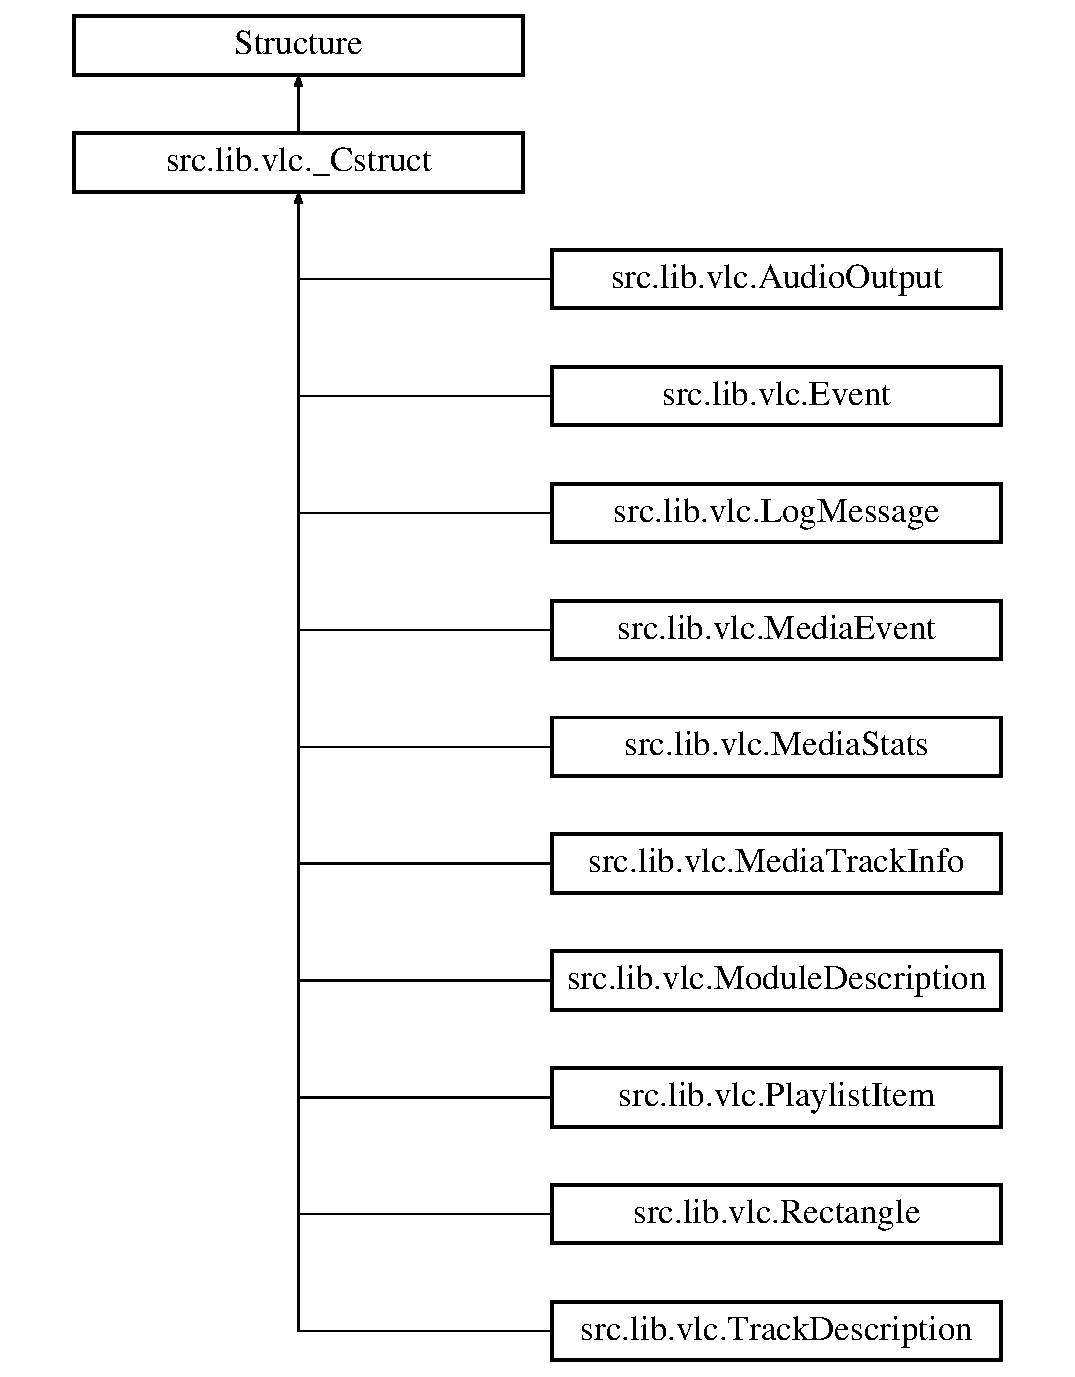
\includegraphics[height=12.000000cm]{classsrc_1_1lib_1_1vlc_1_1__Cstruct}
\end{center}
\end{figure}
\subsection*{Public Member Functions}
\begin{DoxyCompactItemize}
\item 
def \hyperlink{classsrc_1_1lib_1_1vlc_1_1__Cstruct_aa16823982fa22c371ef8b42be32a1196}{\+\_\+\+\_\+str\+\_\+\+\_\+} (self)
\item 
def \hyperlink{classsrc_1_1lib_1_1vlc_1_1__Cstruct_a342ce090e21ebd7ab2a76ab96c5f14a6}{\+\_\+\+\_\+repr\+\_\+\+\_\+} (self)
\end{DoxyCompactItemize}
\subsection*{Static Private Attributes}
\begin{DoxyCompactItemize}
\item 
list \hyperlink{classsrc_1_1lib_1_1vlc_1_1__Cstruct_a6503fe1f19dd39cab7b175dd1cf11e8a}{\+\_\+fields\+\_\+} = \mbox{[}$\,$\mbox{]}
\end{DoxyCompactItemize}


\subsection{Detailed Description}
\begin{DoxyVerb}(INTERNAL) Base class for ctypes structures.
\end{DoxyVerb}
 

\subsection{Member Function Documentation}
\hypertarget{classsrc_1_1lib_1_1vlc_1_1__Cstruct_a342ce090e21ebd7ab2a76ab96c5f14a6}{}\index{src\+::lib\+::vlc\+::\+\_\+\+Cstruct@{src\+::lib\+::vlc\+::\+\_\+\+Cstruct}!\+\_\+\+\_\+repr\+\_\+\+\_\+@{\+\_\+\+\_\+repr\+\_\+\+\_\+}}
\index{\+\_\+\+\_\+repr\+\_\+\+\_\+@{\+\_\+\+\_\+repr\+\_\+\+\_\+}!src\+::lib\+::vlc\+::\+\_\+\+Cstruct@{src\+::lib\+::vlc\+::\+\_\+\+Cstruct}}
\subsubsection[{\+\_\+\+\_\+repr\+\_\+\+\_\+}]{\setlength{\rightskip}{0pt plus 5cm}def src.\+lib.\+vlc.\+\_\+\+Cstruct.\+\_\+\+\_\+repr\+\_\+\+\_\+ (
\begin{DoxyParamCaption}
\item[{}]{self}
\end{DoxyParamCaption}
)}\label{classsrc_1_1lib_1_1vlc_1_1__Cstruct_a342ce090e21ebd7ab2a76ab96c5f14a6}
\hypertarget{classsrc_1_1lib_1_1vlc_1_1__Cstruct_aa16823982fa22c371ef8b42be32a1196}{}\index{src\+::lib\+::vlc\+::\+\_\+\+Cstruct@{src\+::lib\+::vlc\+::\+\_\+\+Cstruct}!\+\_\+\+\_\+str\+\_\+\+\_\+@{\+\_\+\+\_\+str\+\_\+\+\_\+}}
\index{\+\_\+\+\_\+str\+\_\+\+\_\+@{\+\_\+\+\_\+str\+\_\+\+\_\+}!src\+::lib\+::vlc\+::\+\_\+\+Cstruct@{src\+::lib\+::vlc\+::\+\_\+\+Cstruct}}
\subsubsection[{\+\_\+\+\_\+str\+\_\+\+\_\+}]{\setlength{\rightskip}{0pt plus 5cm}def src.\+lib.\+vlc.\+\_\+\+Cstruct.\+\_\+\+\_\+str\+\_\+\+\_\+ (
\begin{DoxyParamCaption}
\item[{}]{self}
\end{DoxyParamCaption}
)}\label{classsrc_1_1lib_1_1vlc_1_1__Cstruct_aa16823982fa22c371ef8b42be32a1196}


\subsection{Member Data Documentation}
\hypertarget{classsrc_1_1lib_1_1vlc_1_1__Cstruct_a6503fe1f19dd39cab7b175dd1cf11e8a}{}\index{src\+::lib\+::vlc\+::\+\_\+\+Cstruct@{src\+::lib\+::vlc\+::\+\_\+\+Cstruct}!\+\_\+fields\+\_\+@{\+\_\+fields\+\_\+}}
\index{\+\_\+fields\+\_\+@{\+\_\+fields\+\_\+}!src\+::lib\+::vlc\+::\+\_\+\+Cstruct@{src\+::lib\+::vlc\+::\+\_\+\+Cstruct}}
\subsubsection[{\+\_\+fields\+\_\+}]{\setlength{\rightskip}{0pt plus 5cm}list src.\+lib.\+vlc.\+\_\+\+Cstruct.\+\_\+fields\+\_\+ = \mbox{[}$\,$\mbox{]}\hspace{0.3cm}{\ttfamily [static]}, {\ttfamily [private]}}\label{classsrc_1_1lib_1_1vlc_1_1__Cstruct_a6503fe1f19dd39cab7b175dd1cf11e8a}


The documentation for this class was generated from the following file\+:\begin{DoxyCompactItemize}
\item 
src/lib/\hyperlink{vlc_8py}{vlc.\+py}\end{DoxyCompactItemize}

\hypertarget{classsrc_1_1lib_1_1vlc_1_1__Ctype}{}\section{src.\+lib.\+vlc.\+\_\+\+Ctype Class Reference}
\label{classsrc_1_1lib_1_1vlc_1_1__Ctype}\index{src.\+lib.\+vlc.\+\_\+\+Ctype@{src.\+lib.\+vlc.\+\_\+\+Ctype}}
Inheritance diagram for src.\+lib.\+vlc.\+\_\+\+Ctype\+:\begin{figure}[H]
\begin{center}
\leavevmode
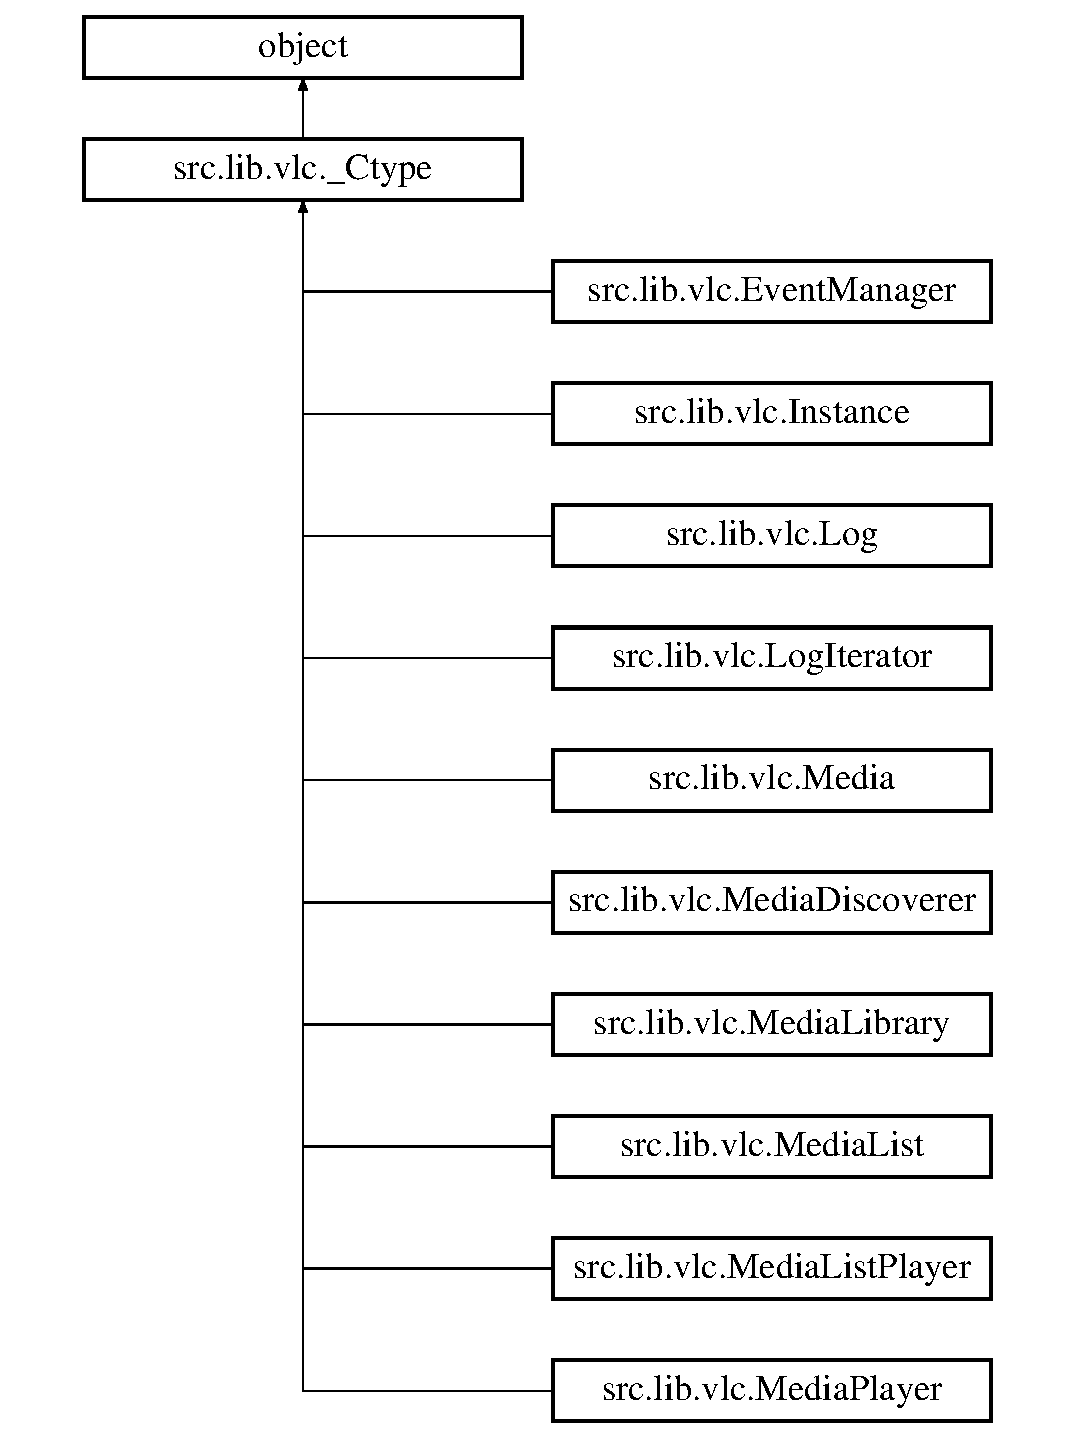
\includegraphics[height=12.000000cm]{classsrc_1_1lib_1_1vlc_1_1__Ctype}
\end{center}
\end{figure}
\subsection*{Static Public Member Functions}
\begin{DoxyCompactItemize}
\item 
def \hyperlink{classsrc_1_1lib_1_1vlc_1_1__Ctype_a607ac5511a14b6f4a00f3d50e6c9669c}{from\+\_\+param} (this)
\end{DoxyCompactItemize}


\subsection{Detailed Description}
\begin{DoxyVerb}(INTERNAL) Base class for ctypes.
\end{DoxyVerb}
 

\subsection{Member Function Documentation}
\hypertarget{classsrc_1_1lib_1_1vlc_1_1__Ctype_a607ac5511a14b6f4a00f3d50e6c9669c}{}\index{src\+::lib\+::vlc\+::\+\_\+\+Ctype@{src\+::lib\+::vlc\+::\+\_\+\+Ctype}!from\+\_\+param@{from\+\_\+param}}
\index{from\+\_\+param@{from\+\_\+param}!src\+::lib\+::vlc\+::\+\_\+\+Ctype@{src\+::lib\+::vlc\+::\+\_\+\+Ctype}}
\subsubsection[{from\+\_\+param}]{\setlength{\rightskip}{0pt plus 5cm}def src.\+lib.\+vlc.\+\_\+\+Ctype.\+from\+\_\+param (
\begin{DoxyParamCaption}
\item[{}]{this}
\end{DoxyParamCaption}
)\hspace{0.3cm}{\ttfamily [static]}}\label{classsrc_1_1lib_1_1vlc_1_1__Ctype_a607ac5511a14b6f4a00f3d50e6c9669c}
\begin{DoxyVerb}(INTERNAL) ctypes parameter conversion method.
\end{DoxyVerb}
 

The documentation for this class was generated from the following file\+:\begin{DoxyCompactItemize}
\item 
src/lib/\hyperlink{vlc_8py}{vlc.\+py}\end{DoxyCompactItemize}

\hypertarget{classsrc_1_1lib_1_1vlc_1_1__Enum}{}\section{src.\+lib.\+vlc.\+\_\+\+Enum Class Reference}
\label{classsrc_1_1lib_1_1vlc_1_1__Enum}\index{src.\+lib.\+vlc.\+\_\+\+Enum@{src.\+lib.\+vlc.\+\_\+\+Enum}}
Inheritance diagram for src.\+lib.\+vlc.\+\_\+\+Enum\+:\begin{figure}[H]
\begin{center}
\leavevmode
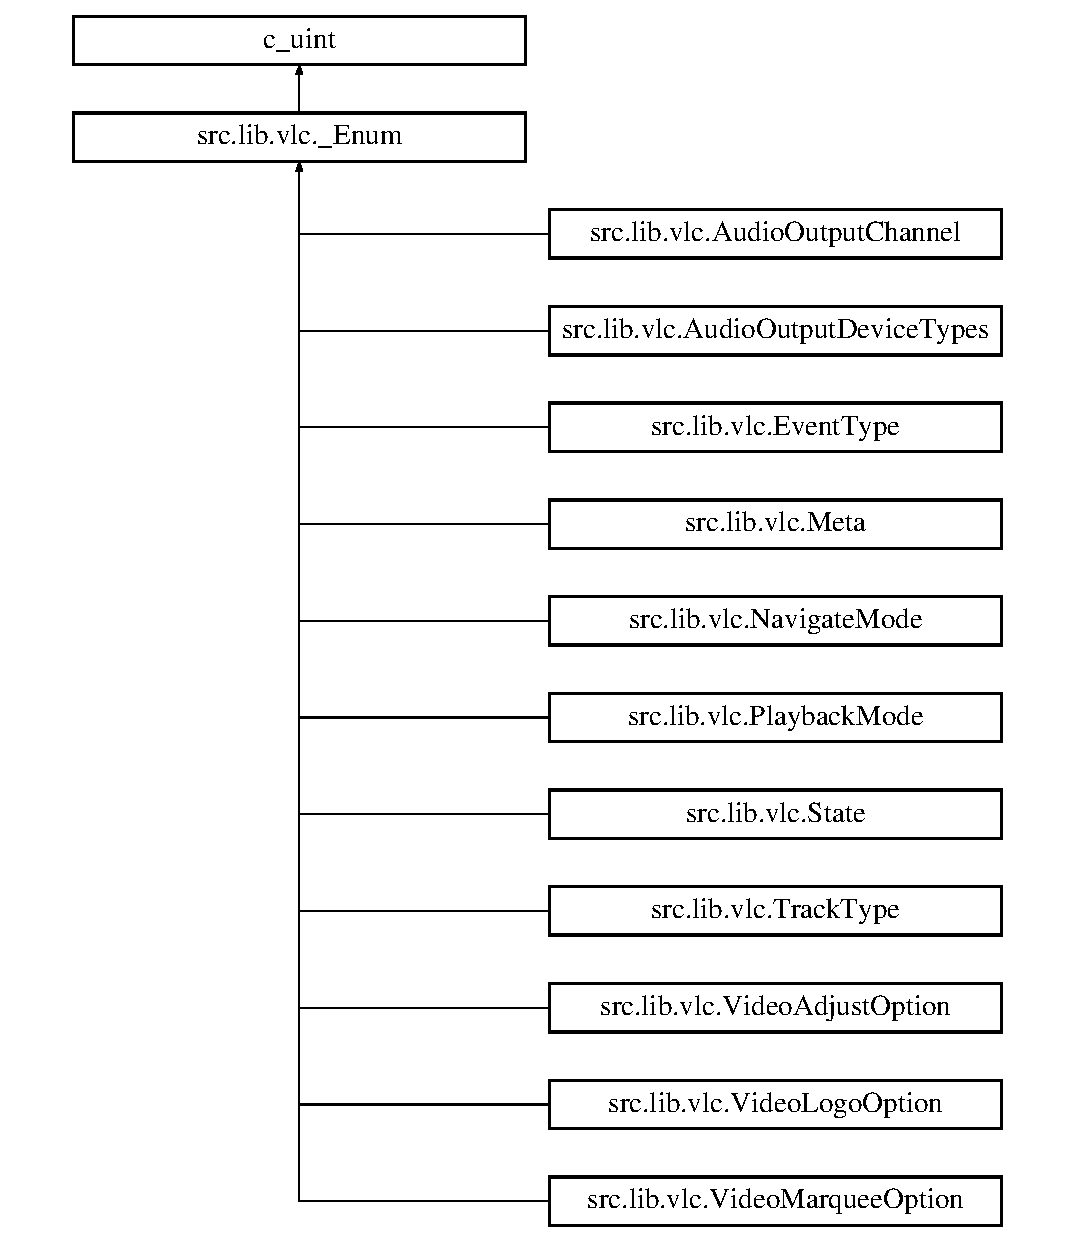
\includegraphics[height=12.000000cm]{classsrc_1_1lib_1_1vlc_1_1__Enum}
\end{center}
\end{figure}
\subsection*{Public Member Functions}
\begin{DoxyCompactItemize}
\item 
def \hyperlink{classsrc_1_1lib_1_1vlc_1_1__Enum_a8ee3332104c851d949ba733cc5ef4b2c}{\+\_\+\+\_\+str\+\_\+\+\_\+} (self)
\item 
def \hyperlink{classsrc_1_1lib_1_1vlc_1_1__Enum_aa6dce4015a93caccc6e679fe5517c2a6}{\+\_\+\+\_\+repr\+\_\+\+\_\+} (self)
\item 
def \hyperlink{classsrc_1_1lib_1_1vlc_1_1__Enum_a0f47c8262d9cd976a021424c28733fab}{\+\_\+\+\_\+eq\+\_\+\+\_\+} (self, other)
\item 
def \hyperlink{classsrc_1_1lib_1_1vlc_1_1__Enum_aeaad711ab3794d8453ed172ce6adcbe4}{\+\_\+\+\_\+ne\+\_\+\+\_\+} (self, other)
\end{DoxyCompactItemize}
\subsection*{Public Attributes}
\begin{DoxyCompactItemize}
\item 
\hyperlink{classsrc_1_1lib_1_1vlc_1_1__Enum_abf044fdbcc58c25961d92b97a3c98eca}{value}
\end{DoxyCompactItemize}
\subsection*{Static Private Attributes}
\begin{DoxyCompactItemize}
\item 
dictionary \hyperlink{classsrc_1_1lib_1_1vlc_1_1__Enum_a72ea675c63b9b3d93bd5f1d8cbde8fcb}{\+\_\+enum\+\_\+names\+\_\+} = \{\}
\end{DoxyCompactItemize}


\subsection{Detailed Description}
\begin{DoxyVerb}(INTERNAL) Base class
\end{DoxyVerb}
 

\subsection{Member Function Documentation}
\hypertarget{classsrc_1_1lib_1_1vlc_1_1__Enum_a0f47c8262d9cd976a021424c28733fab}{}\index{src\+::lib\+::vlc\+::\+\_\+\+Enum@{src\+::lib\+::vlc\+::\+\_\+\+Enum}!\+\_\+\+\_\+eq\+\_\+\+\_\+@{\+\_\+\+\_\+eq\+\_\+\+\_\+}}
\index{\+\_\+\+\_\+eq\+\_\+\+\_\+@{\+\_\+\+\_\+eq\+\_\+\+\_\+}!src\+::lib\+::vlc\+::\+\_\+\+Enum@{src\+::lib\+::vlc\+::\+\_\+\+Enum}}
\subsubsection[{\+\_\+\+\_\+eq\+\_\+\+\_\+}]{\setlength{\rightskip}{0pt plus 5cm}def src.\+lib.\+vlc.\+\_\+\+Enum.\+\_\+\+\_\+eq\+\_\+\+\_\+ (
\begin{DoxyParamCaption}
\item[{}]{self, }
\item[{}]{other}
\end{DoxyParamCaption}
)}\label{classsrc_1_1lib_1_1vlc_1_1__Enum_a0f47c8262d9cd976a021424c28733fab}
\hypertarget{classsrc_1_1lib_1_1vlc_1_1__Enum_aeaad711ab3794d8453ed172ce6adcbe4}{}\index{src\+::lib\+::vlc\+::\+\_\+\+Enum@{src\+::lib\+::vlc\+::\+\_\+\+Enum}!\+\_\+\+\_\+ne\+\_\+\+\_\+@{\+\_\+\+\_\+ne\+\_\+\+\_\+}}
\index{\+\_\+\+\_\+ne\+\_\+\+\_\+@{\+\_\+\+\_\+ne\+\_\+\+\_\+}!src\+::lib\+::vlc\+::\+\_\+\+Enum@{src\+::lib\+::vlc\+::\+\_\+\+Enum}}
\subsubsection[{\+\_\+\+\_\+ne\+\_\+\+\_\+}]{\setlength{\rightskip}{0pt plus 5cm}def src.\+lib.\+vlc.\+\_\+\+Enum.\+\_\+\+\_\+ne\+\_\+\+\_\+ (
\begin{DoxyParamCaption}
\item[{}]{self, }
\item[{}]{other}
\end{DoxyParamCaption}
)}\label{classsrc_1_1lib_1_1vlc_1_1__Enum_aeaad711ab3794d8453ed172ce6adcbe4}
\hypertarget{classsrc_1_1lib_1_1vlc_1_1__Enum_aa6dce4015a93caccc6e679fe5517c2a6}{}\index{src\+::lib\+::vlc\+::\+\_\+\+Enum@{src\+::lib\+::vlc\+::\+\_\+\+Enum}!\+\_\+\+\_\+repr\+\_\+\+\_\+@{\+\_\+\+\_\+repr\+\_\+\+\_\+}}
\index{\+\_\+\+\_\+repr\+\_\+\+\_\+@{\+\_\+\+\_\+repr\+\_\+\+\_\+}!src\+::lib\+::vlc\+::\+\_\+\+Enum@{src\+::lib\+::vlc\+::\+\_\+\+Enum}}
\subsubsection[{\+\_\+\+\_\+repr\+\_\+\+\_\+}]{\setlength{\rightskip}{0pt plus 5cm}def src.\+lib.\+vlc.\+\_\+\+Enum.\+\_\+\+\_\+repr\+\_\+\+\_\+ (
\begin{DoxyParamCaption}
\item[{}]{self}
\end{DoxyParamCaption}
)}\label{classsrc_1_1lib_1_1vlc_1_1__Enum_aa6dce4015a93caccc6e679fe5517c2a6}
\hypertarget{classsrc_1_1lib_1_1vlc_1_1__Enum_a8ee3332104c851d949ba733cc5ef4b2c}{}\index{src\+::lib\+::vlc\+::\+\_\+\+Enum@{src\+::lib\+::vlc\+::\+\_\+\+Enum}!\+\_\+\+\_\+str\+\_\+\+\_\+@{\+\_\+\+\_\+str\+\_\+\+\_\+}}
\index{\+\_\+\+\_\+str\+\_\+\+\_\+@{\+\_\+\+\_\+str\+\_\+\+\_\+}!src\+::lib\+::vlc\+::\+\_\+\+Enum@{src\+::lib\+::vlc\+::\+\_\+\+Enum}}
\subsubsection[{\+\_\+\+\_\+str\+\_\+\+\_\+}]{\setlength{\rightskip}{0pt plus 5cm}def src.\+lib.\+vlc.\+\_\+\+Enum.\+\_\+\+\_\+str\+\_\+\+\_\+ (
\begin{DoxyParamCaption}
\item[{}]{self}
\end{DoxyParamCaption}
)}\label{classsrc_1_1lib_1_1vlc_1_1__Enum_a8ee3332104c851d949ba733cc5ef4b2c}


\subsection{Member Data Documentation}
\hypertarget{classsrc_1_1lib_1_1vlc_1_1__Enum_a72ea675c63b9b3d93bd5f1d8cbde8fcb}{}\index{src\+::lib\+::vlc\+::\+\_\+\+Enum@{src\+::lib\+::vlc\+::\+\_\+\+Enum}!\+\_\+enum\+\_\+names\+\_\+@{\+\_\+enum\+\_\+names\+\_\+}}
\index{\+\_\+enum\+\_\+names\+\_\+@{\+\_\+enum\+\_\+names\+\_\+}!src\+::lib\+::vlc\+::\+\_\+\+Enum@{src\+::lib\+::vlc\+::\+\_\+\+Enum}}
\subsubsection[{\+\_\+enum\+\_\+names\+\_\+}]{\setlength{\rightskip}{0pt plus 5cm}dictionary src.\+lib.\+vlc.\+\_\+\+Enum.\+\_\+enum\+\_\+names\+\_\+ = \{\}\hspace{0.3cm}{\ttfamily [static]}, {\ttfamily [private]}}\label{classsrc_1_1lib_1_1vlc_1_1__Enum_a72ea675c63b9b3d93bd5f1d8cbde8fcb}
\hypertarget{classsrc_1_1lib_1_1vlc_1_1__Enum_abf044fdbcc58c25961d92b97a3c98eca}{}\index{src\+::lib\+::vlc\+::\+\_\+\+Enum@{src\+::lib\+::vlc\+::\+\_\+\+Enum}!value@{value}}
\index{value@{value}!src\+::lib\+::vlc\+::\+\_\+\+Enum@{src\+::lib\+::vlc\+::\+\_\+\+Enum}}
\subsubsection[{value}]{\setlength{\rightskip}{0pt plus 5cm}src.\+lib.\+vlc.\+\_\+\+Enum.\+value}\label{classsrc_1_1lib_1_1vlc_1_1__Enum_abf044fdbcc58c25961d92b97a3c98eca}


The documentation for this class was generated from the following file\+:\begin{DoxyCompactItemize}
\item 
src/lib/\hyperlink{vlc_8py}{vlc.\+py}\end{DoxyCompactItemize}

\hypertarget{classsrc_1_1lib_1_1vlc_1_1AudioOutput}{}\section{src.\+lib.\+vlc.\+Audio\+Output Class Reference}
\label{classsrc_1_1lib_1_1vlc_1_1AudioOutput}\index{src.\+lib.\+vlc.\+Audio\+Output@{src.\+lib.\+vlc.\+Audio\+Output}}
Inheritance diagram for src.\+lib.\+vlc.\+Audio\+Output\+:\begin{figure}[H]
\begin{center}
\leavevmode
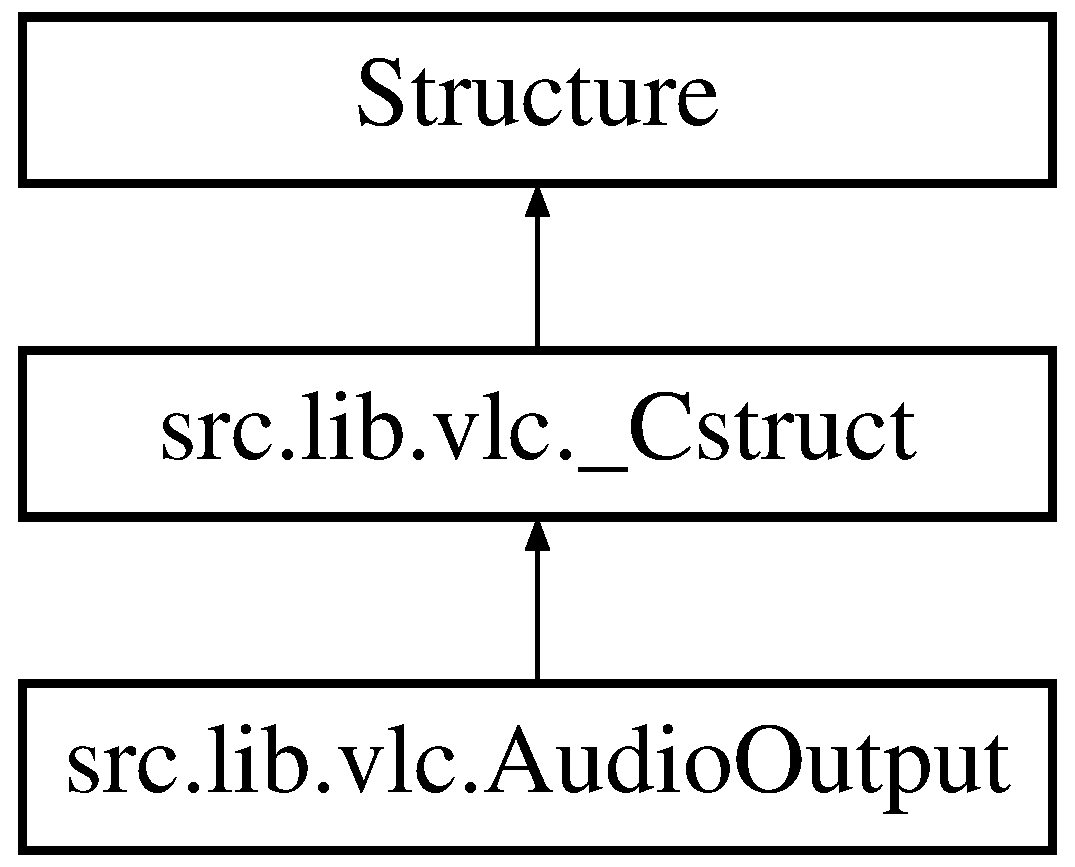
\includegraphics[height=3.000000cm]{classsrc_1_1lib_1_1vlc_1_1AudioOutput}
\end{center}
\end{figure}
\subsection*{Public Member Functions}
\begin{DoxyCompactItemize}
\item 
def \hyperlink{classsrc_1_1lib_1_1vlc_1_1AudioOutput_a909a740bb0c646b9e7aa54bc6c5f7334}{\+\_\+\+\_\+str\+\_\+\+\_\+} (self)
\end{DoxyCompactItemize}


\subsection{Member Function Documentation}
\hypertarget{classsrc_1_1lib_1_1vlc_1_1AudioOutput_a909a740bb0c646b9e7aa54bc6c5f7334}{}\index{src\+::lib\+::vlc\+::\+Audio\+Output@{src\+::lib\+::vlc\+::\+Audio\+Output}!\+\_\+\+\_\+str\+\_\+\+\_\+@{\+\_\+\+\_\+str\+\_\+\+\_\+}}
\index{\+\_\+\+\_\+str\+\_\+\+\_\+@{\+\_\+\+\_\+str\+\_\+\+\_\+}!src\+::lib\+::vlc\+::\+Audio\+Output@{src\+::lib\+::vlc\+::\+Audio\+Output}}
\subsubsection[{\+\_\+\+\_\+str\+\_\+\+\_\+}]{\setlength{\rightskip}{0pt plus 5cm}def src.\+lib.\+vlc.\+Audio\+Output.\+\_\+\+\_\+str\+\_\+\+\_\+ (
\begin{DoxyParamCaption}
\item[{}]{self}
\end{DoxyParamCaption}
)}\label{classsrc_1_1lib_1_1vlc_1_1AudioOutput_a909a740bb0c646b9e7aa54bc6c5f7334}


The documentation for this class was generated from the following file\+:\begin{DoxyCompactItemize}
\item 
src/lib/\hyperlink{vlc_8py}{vlc.\+py}\end{DoxyCompactItemize}

\hypertarget{classsrc_1_1lib_1_1vlc_1_1AudioOutputChannel}{}\section{src.\+lib.\+vlc.\+Audio\+Output\+Channel Class Reference}
\label{classsrc_1_1lib_1_1vlc_1_1AudioOutputChannel}\index{src.\+lib.\+vlc.\+Audio\+Output\+Channel@{src.\+lib.\+vlc.\+Audio\+Output\+Channel}}
Inheritance diagram for src.\+lib.\+vlc.\+Audio\+Output\+Channel\+:\begin{figure}[H]
\begin{center}
\leavevmode
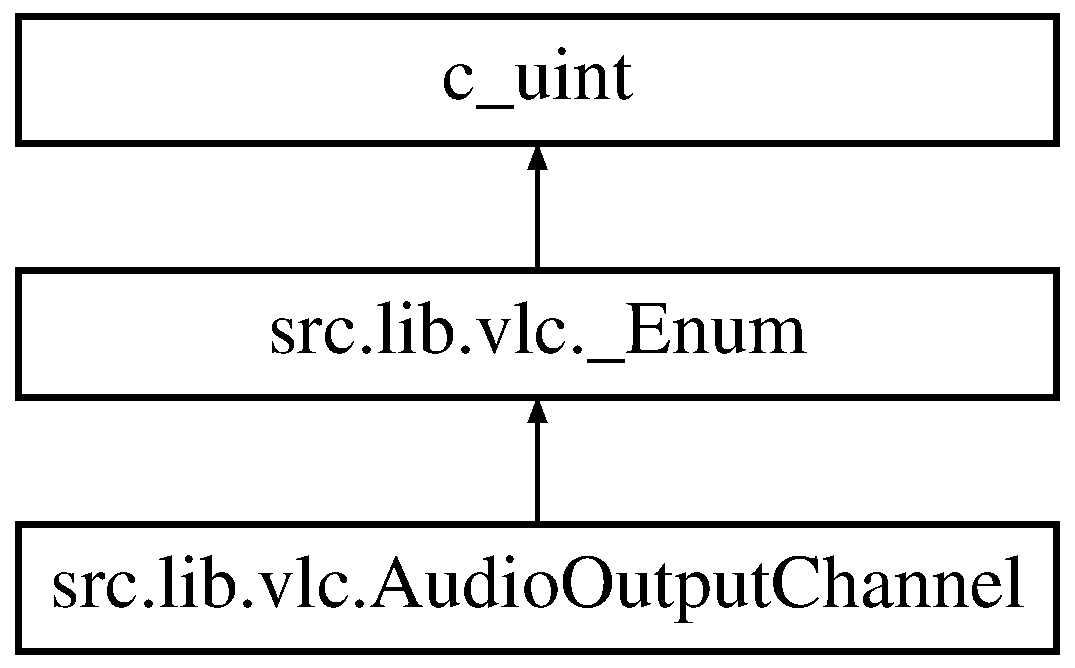
\includegraphics[height=3.000000cm]{classsrc_1_1lib_1_1vlc_1_1AudioOutputChannel}
\end{center}
\end{figure}
\subsection*{Static Private Attributes}
\begin{DoxyCompactItemize}
\item 
dictionary \hyperlink{classsrc_1_1lib_1_1vlc_1_1AudioOutputChannel_ade28d35cc14a39eefc1054be45624e3e}{\+\_\+enum\+\_\+names\+\_\+}
\end{DoxyCompactItemize}
\subsection*{Additional Inherited Members}


\subsection{Detailed Description}
\begin{DoxyVerb}Audio channels.
\end{DoxyVerb}
 

\subsection{Member Data Documentation}
\hypertarget{classsrc_1_1lib_1_1vlc_1_1AudioOutputChannel_ade28d35cc14a39eefc1054be45624e3e}{}\index{src\+::lib\+::vlc\+::\+Audio\+Output\+Channel@{src\+::lib\+::vlc\+::\+Audio\+Output\+Channel}!\+\_\+enum\+\_\+names\+\_\+@{\+\_\+enum\+\_\+names\+\_\+}}
\index{\+\_\+enum\+\_\+names\+\_\+@{\+\_\+enum\+\_\+names\+\_\+}!src\+::lib\+::vlc\+::\+Audio\+Output\+Channel@{src\+::lib\+::vlc\+::\+Audio\+Output\+Channel}}
\subsubsection[{\+\_\+enum\+\_\+names\+\_\+}]{\setlength{\rightskip}{0pt plus 5cm}dictionary src.\+lib.\+vlc.\+Audio\+Output\+Channel.\+\_\+enum\+\_\+names\+\_\+\hspace{0.3cm}{\ttfamily [static]}, {\ttfamily [private]}}\label{classsrc_1_1lib_1_1vlc_1_1AudioOutputChannel_ade28d35cc14a39eefc1054be45624e3e}
{\bfseries Initial value\+:}
\begin{DoxyCode}
1 = \{
2         -1: \textcolor{stringliteral}{'Error'},
3         1: \textcolor{stringliteral}{'Stereo'},
4         2: \textcolor{stringliteral}{'RStereo'},
5         3: \textcolor{stringliteral}{'Left'},
6         4: \textcolor{stringliteral}{'Right'},
7         5: \textcolor{stringliteral}{'Dolbys'},
8     \}
\end{DoxyCode}


The documentation for this class was generated from the following file\+:\begin{DoxyCompactItemize}
\item 
src/lib/\hyperlink{vlc_8py}{vlc.\+py}\end{DoxyCompactItemize}

\hypertarget{classsrc_1_1lib_1_1vlc_1_1AudioOutputDeviceTypes}{}\section{src.\+lib.\+vlc.\+Audio\+Output\+Device\+Types Class Reference}
\label{classsrc_1_1lib_1_1vlc_1_1AudioOutputDeviceTypes}\index{src.\+lib.\+vlc.\+Audio\+Output\+Device\+Types@{src.\+lib.\+vlc.\+Audio\+Output\+Device\+Types}}
Inheritance diagram for src.\+lib.\+vlc.\+Audio\+Output\+Device\+Types\+:\begin{figure}[H]
\begin{center}
\leavevmode
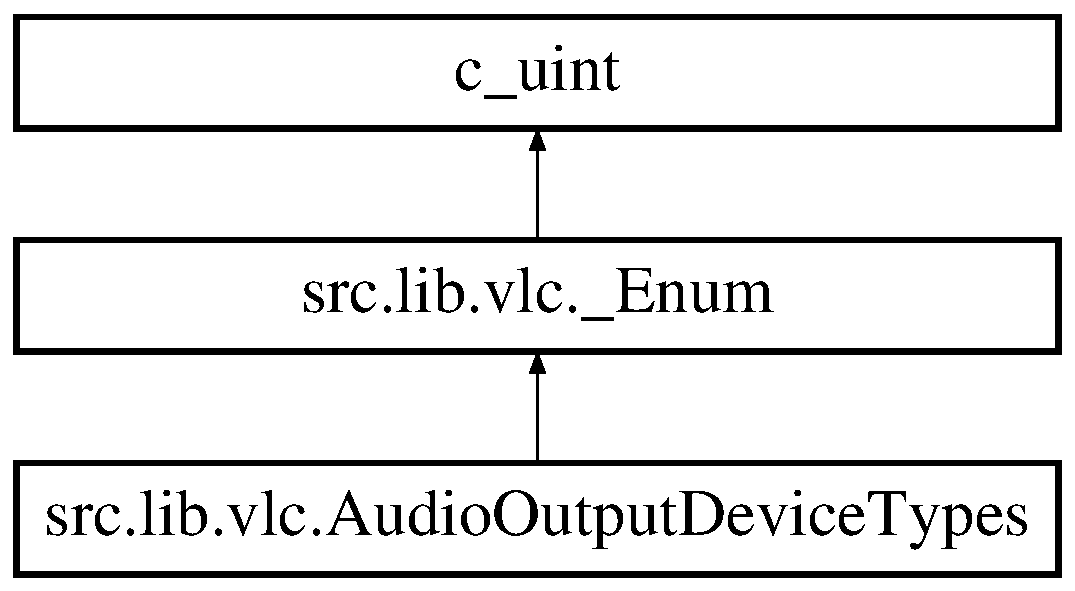
\includegraphics[height=3.000000cm]{classsrc_1_1lib_1_1vlc_1_1AudioOutputDeviceTypes}
\end{center}
\end{figure}
\subsection*{Static Private Attributes}
\begin{DoxyCompactItemize}
\item 
dictionary \hyperlink{classsrc_1_1lib_1_1vlc_1_1AudioOutputDeviceTypes_a8a1417d077523d4052c95707a6f1a16d}{\+\_\+enum\+\_\+names\+\_\+}
\end{DoxyCompactItemize}
\subsection*{Additional Inherited Members}


\subsection{Detailed Description}
\begin{DoxyVerb}Audio device types.
\end{DoxyVerb}
 

\subsection{Member Data Documentation}
\hypertarget{classsrc_1_1lib_1_1vlc_1_1AudioOutputDeviceTypes_a8a1417d077523d4052c95707a6f1a16d}{}\index{src\+::lib\+::vlc\+::\+Audio\+Output\+Device\+Types@{src\+::lib\+::vlc\+::\+Audio\+Output\+Device\+Types}!\+\_\+enum\+\_\+names\+\_\+@{\+\_\+enum\+\_\+names\+\_\+}}
\index{\+\_\+enum\+\_\+names\+\_\+@{\+\_\+enum\+\_\+names\+\_\+}!src\+::lib\+::vlc\+::\+Audio\+Output\+Device\+Types@{src\+::lib\+::vlc\+::\+Audio\+Output\+Device\+Types}}
\subsubsection[{\+\_\+enum\+\_\+names\+\_\+}]{\setlength{\rightskip}{0pt plus 5cm}dictionary src.\+lib.\+vlc.\+Audio\+Output\+Device\+Types.\+\_\+enum\+\_\+names\+\_\+\hspace{0.3cm}{\ttfamily [static]}, {\ttfamily [private]}}\label{classsrc_1_1lib_1_1vlc_1_1AudioOutputDeviceTypes_a8a1417d077523d4052c95707a6f1a16d}
{\bfseries Initial value\+:}
\begin{DoxyCode}
1 = \{
2         -1: \textcolor{stringliteral}{'Error'},
3         1: \textcolor{stringliteral}{'Mono'},
4         2: \textcolor{stringliteral}{'Stereo'},
5         4: \textcolor{stringliteral}{'\_2F2R'},
6         5: \textcolor{stringliteral}{'\_3F2R'},
7         6: \textcolor{stringliteral}{'\_5\_1'},
8         7: \textcolor{stringliteral}{'\_6\_1'},
9         8: \textcolor{stringliteral}{'\_7\_1'},
10         10: \textcolor{stringliteral}{'SPDIF'},
11     \}
\end{DoxyCode}


The documentation for this class was generated from the following file\+:\begin{DoxyCompactItemize}
\item 
src/lib/\hyperlink{vlc_8py}{vlc.\+py}\end{DoxyCompactItemize}

\hypertarget{classsrc_1_1adapter_1_1buffering__adapter_1_1Buffering__Adapter}{}\section{src.\+adapter.\+buffering\+\_\+adapter.\+Buffering\+\_\+\+Adapter Class Reference}
\label{classsrc_1_1adapter_1_1buffering__adapter_1_1Buffering__Adapter}\index{src.\+adapter.\+buffering\+\_\+adapter.\+Buffering\+\_\+\+Adapter@{src.\+adapter.\+buffering\+\_\+adapter.\+Buffering\+\_\+\+Adapter}}
\subsection*{Public Member Functions}
\begin{DoxyCompactItemize}
\item 
def \hyperlink{classsrc_1_1adapter_1_1buffering__adapter_1_1Buffering__Adapter_a44774d27991c6242887e0c1c6c51ee59}{set\+\_\+widget} (self, progress\+\_\+bar)
\end{DoxyCompactItemize}
\subsection*{Static Public Attributes}
\begin{DoxyCompactItemize}
\item 
\hyperlink{classsrc_1_1adapter_1_1buffering__adapter_1_1Buffering__Adapter_ac7a3269ffd08f8f1dd5f93b5442b2a73}{W\+I\+D\+G\+E\+T} = None
\end{DoxyCompactItemize}


\subsection{Member Function Documentation}
\hypertarget{classsrc_1_1adapter_1_1buffering__adapter_1_1Buffering__Adapter_a44774d27991c6242887e0c1c6c51ee59}{}\index{src\+::adapter\+::buffering\+\_\+adapter\+::\+Buffering\+\_\+\+Adapter@{src\+::adapter\+::buffering\+\_\+adapter\+::\+Buffering\+\_\+\+Adapter}!set\+\_\+widget@{set\+\_\+widget}}
\index{set\+\_\+widget@{set\+\_\+widget}!src\+::adapter\+::buffering\+\_\+adapter\+::\+Buffering\+\_\+\+Adapter@{src\+::adapter\+::buffering\+\_\+adapter\+::\+Buffering\+\_\+\+Adapter}}
\subsubsection[{set\+\_\+widget}]{\setlength{\rightskip}{0pt plus 5cm}def src.\+adapter.\+buffering\+\_\+adapter.\+Buffering\+\_\+\+Adapter.\+set\+\_\+widget (
\begin{DoxyParamCaption}
\item[{}]{self, }
\item[{}]{progress\+\_\+bar}
\end{DoxyParamCaption}
)}\label{classsrc_1_1adapter_1_1buffering__adapter_1_1Buffering__Adapter_a44774d27991c6242887e0c1c6c51ee59}


\subsection{Member Data Documentation}
\hypertarget{classsrc_1_1adapter_1_1buffering__adapter_1_1Buffering__Adapter_ac7a3269ffd08f8f1dd5f93b5442b2a73}{}\index{src\+::adapter\+::buffering\+\_\+adapter\+::\+Buffering\+\_\+\+Adapter@{src\+::adapter\+::buffering\+\_\+adapter\+::\+Buffering\+\_\+\+Adapter}!W\+I\+D\+G\+E\+T@{W\+I\+D\+G\+E\+T}}
\index{W\+I\+D\+G\+E\+T@{W\+I\+D\+G\+E\+T}!src\+::adapter\+::buffering\+\_\+adapter\+::\+Buffering\+\_\+\+Adapter@{src\+::adapter\+::buffering\+\_\+adapter\+::\+Buffering\+\_\+\+Adapter}}
\subsubsection[{W\+I\+D\+G\+E\+T}]{\setlength{\rightskip}{0pt plus 5cm}src.\+adapter.\+buffering\+\_\+adapter.\+Buffering\+\_\+\+Adapter.\+W\+I\+D\+G\+E\+T = None\hspace{0.3cm}{\ttfamily [static]}}\label{classsrc_1_1adapter_1_1buffering__adapter_1_1Buffering__Adapter_ac7a3269ffd08f8f1dd5f93b5442b2a73}


The documentation for this class was generated from the following file\+:\begin{DoxyCompactItemize}
\item 
src/adapter/\hyperlink{buffering__adapter_8py}{buffering\+\_\+adapter.\+py}\end{DoxyCompactItemize}

\hypertarget{classsrc_1_1model_1_1category_1_1Category}{}\section{src.\+model.\+category.\+Category Class Reference}
\label{classsrc_1_1model_1_1category_1_1Category}\index{src.\+model.\+category.\+Category@{src.\+model.\+category.\+Category}}
\subsection*{Public Member Functions}
\begin{DoxyCompactItemize}
\item 
def \hyperlink{classsrc_1_1model_1_1category_1_1Category_a42428a103608c2235a080796311229df}{\+\_\+\+\_\+init\+\_\+\+\_\+} (self, \hyperlink{classsrc_1_1model_1_1category_1_1Category_ac1f8913b5d11d768cb48cde2760f8322}{name})
\item 
def \hyperlink{classsrc_1_1model_1_1category_1_1Category_a9ab7071a70ec03d354867d45c2fc3430}{get\+\_\+channels} (self)
\item 
def \hyperlink{classsrc_1_1model_1_1category_1_1Category_a78262aabd6177a36f263b951622f8793}{set\+\_\+name} (self, \hyperlink{classsrc_1_1model_1_1category_1_1Category_ac1f8913b5d11d768cb48cde2760f8322}{name})
\item 
def \hyperlink{classsrc_1_1model_1_1category_1_1Category_abd572aca2e8c0366b8f9e501854631b0}{get\+\_\+name} (self)
\item 
def \hyperlink{classsrc_1_1model_1_1category_1_1Category_a76e9ca634460246d112f3c82e1049975}{add} (self, key, channel)
\item 
def \hyperlink{classsrc_1_1model_1_1category_1_1Category_a463fdbd98805904b49740915d541352f}{remove} (self, key)
\item 
def \hyperlink{classsrc_1_1model_1_1category_1_1Category_a93a44556d4e18dd423a167389f9b98ab}{get\+\_\+channel} (self, key)
\end{DoxyCompactItemize}
\subsection*{Public Attributes}
\begin{DoxyCompactItemize}
\item 
\hyperlink{classsrc_1_1model_1_1category_1_1Category_ac1f8913b5d11d768cb48cde2760f8322}{name}
\item 
\hyperlink{classsrc_1_1model_1_1category_1_1Category_af7b8a88e3eda96fa9bf9cb8c110800b3}{channels}
\end{DoxyCompactItemize}


\subsection{Constructor \& Destructor Documentation}
\hypertarget{classsrc_1_1model_1_1category_1_1Category_a42428a103608c2235a080796311229df}{}\index{src\+::model\+::category\+::\+Category@{src\+::model\+::category\+::\+Category}!\+\_\+\+\_\+init\+\_\+\+\_\+@{\+\_\+\+\_\+init\+\_\+\+\_\+}}
\index{\+\_\+\+\_\+init\+\_\+\+\_\+@{\+\_\+\+\_\+init\+\_\+\+\_\+}!src\+::model\+::category\+::\+Category@{src\+::model\+::category\+::\+Category}}
\subsubsection[{\+\_\+\+\_\+init\+\_\+\+\_\+}]{\setlength{\rightskip}{0pt plus 5cm}def src.\+model.\+category.\+Category.\+\_\+\+\_\+init\+\_\+\+\_\+ (
\begin{DoxyParamCaption}
\item[{}]{self, }
\item[{}]{name}
\end{DoxyParamCaption}
)}\label{classsrc_1_1model_1_1category_1_1Category_a42428a103608c2235a080796311229df}


\subsection{Member Function Documentation}
\hypertarget{classsrc_1_1model_1_1category_1_1Category_a76e9ca634460246d112f3c82e1049975}{}\index{src\+::model\+::category\+::\+Category@{src\+::model\+::category\+::\+Category}!add@{add}}
\index{add@{add}!src\+::model\+::category\+::\+Category@{src\+::model\+::category\+::\+Category}}
\subsubsection[{add}]{\setlength{\rightskip}{0pt plus 5cm}def src.\+model.\+category.\+Category.\+add (
\begin{DoxyParamCaption}
\item[{}]{self, }
\item[{}]{key, }
\item[{}]{channel}
\end{DoxyParamCaption}
)}\label{classsrc_1_1model_1_1category_1_1Category_a76e9ca634460246d112f3c82e1049975}
\hypertarget{classsrc_1_1model_1_1category_1_1Category_a93a44556d4e18dd423a167389f9b98ab}{}\index{src\+::model\+::category\+::\+Category@{src\+::model\+::category\+::\+Category}!get\+\_\+channel@{get\+\_\+channel}}
\index{get\+\_\+channel@{get\+\_\+channel}!src\+::model\+::category\+::\+Category@{src\+::model\+::category\+::\+Category}}
\subsubsection[{get\+\_\+channel}]{\setlength{\rightskip}{0pt plus 5cm}def src.\+model.\+category.\+Category.\+get\+\_\+channel (
\begin{DoxyParamCaption}
\item[{}]{self, }
\item[{}]{key}
\end{DoxyParamCaption}
)}\label{classsrc_1_1model_1_1category_1_1Category_a93a44556d4e18dd423a167389f9b98ab}
\hypertarget{classsrc_1_1model_1_1category_1_1Category_a9ab7071a70ec03d354867d45c2fc3430}{}\index{src\+::model\+::category\+::\+Category@{src\+::model\+::category\+::\+Category}!get\+\_\+channels@{get\+\_\+channels}}
\index{get\+\_\+channels@{get\+\_\+channels}!src\+::model\+::category\+::\+Category@{src\+::model\+::category\+::\+Category}}
\subsubsection[{get\+\_\+channels}]{\setlength{\rightskip}{0pt plus 5cm}def src.\+model.\+category.\+Category.\+get\+\_\+channels (
\begin{DoxyParamCaption}
\item[{}]{self}
\end{DoxyParamCaption}
)}\label{classsrc_1_1model_1_1category_1_1Category_a9ab7071a70ec03d354867d45c2fc3430}
\hypertarget{classsrc_1_1model_1_1category_1_1Category_abd572aca2e8c0366b8f9e501854631b0}{}\index{src\+::model\+::category\+::\+Category@{src\+::model\+::category\+::\+Category}!get\+\_\+name@{get\+\_\+name}}
\index{get\+\_\+name@{get\+\_\+name}!src\+::model\+::category\+::\+Category@{src\+::model\+::category\+::\+Category}}
\subsubsection[{get\+\_\+name}]{\setlength{\rightskip}{0pt plus 5cm}def src.\+model.\+category.\+Category.\+get\+\_\+name (
\begin{DoxyParamCaption}
\item[{}]{self}
\end{DoxyParamCaption}
)}\label{classsrc_1_1model_1_1category_1_1Category_abd572aca2e8c0366b8f9e501854631b0}
\hypertarget{classsrc_1_1model_1_1category_1_1Category_a463fdbd98805904b49740915d541352f}{}\index{src\+::model\+::category\+::\+Category@{src\+::model\+::category\+::\+Category}!remove@{remove}}
\index{remove@{remove}!src\+::model\+::category\+::\+Category@{src\+::model\+::category\+::\+Category}}
\subsubsection[{remove}]{\setlength{\rightskip}{0pt plus 5cm}def src.\+model.\+category.\+Category.\+remove (
\begin{DoxyParamCaption}
\item[{}]{self, }
\item[{}]{key}
\end{DoxyParamCaption}
)}\label{classsrc_1_1model_1_1category_1_1Category_a463fdbd98805904b49740915d541352f}
\hypertarget{classsrc_1_1model_1_1category_1_1Category_a78262aabd6177a36f263b951622f8793}{}\index{src\+::model\+::category\+::\+Category@{src\+::model\+::category\+::\+Category}!set\+\_\+name@{set\+\_\+name}}
\index{set\+\_\+name@{set\+\_\+name}!src\+::model\+::category\+::\+Category@{src\+::model\+::category\+::\+Category}}
\subsubsection[{set\+\_\+name}]{\setlength{\rightskip}{0pt plus 5cm}def src.\+model.\+category.\+Category.\+set\+\_\+name (
\begin{DoxyParamCaption}
\item[{}]{self, }
\item[{}]{name}
\end{DoxyParamCaption}
)}\label{classsrc_1_1model_1_1category_1_1Category_a78262aabd6177a36f263b951622f8793}


\subsection{Member Data Documentation}
\hypertarget{classsrc_1_1model_1_1category_1_1Category_af7b8a88e3eda96fa9bf9cb8c110800b3}{}\index{src\+::model\+::category\+::\+Category@{src\+::model\+::category\+::\+Category}!channels@{channels}}
\index{channels@{channels}!src\+::model\+::category\+::\+Category@{src\+::model\+::category\+::\+Category}}
\subsubsection[{channels}]{\setlength{\rightskip}{0pt plus 5cm}src.\+model.\+category.\+Category.\+channels}\label{classsrc_1_1model_1_1category_1_1Category_af7b8a88e3eda96fa9bf9cb8c110800b3}
\hypertarget{classsrc_1_1model_1_1category_1_1Category_ac1f8913b5d11d768cb48cde2760f8322}{}\index{src\+::model\+::category\+::\+Category@{src\+::model\+::category\+::\+Category}!name@{name}}
\index{name@{name}!src\+::model\+::category\+::\+Category@{src\+::model\+::category\+::\+Category}}
\subsubsection[{name}]{\setlength{\rightskip}{0pt plus 5cm}src.\+model.\+category.\+Category.\+name}\label{classsrc_1_1model_1_1category_1_1Category_ac1f8913b5d11d768cb48cde2760f8322}


The documentation for this class was generated from the following file\+:\begin{DoxyCompactItemize}
\item 
src/model/\hyperlink{category_8py}{category.\+py}\end{DoxyCompactItemize}

\hypertarget{classsrc_1_1model_1_1channel_1_1Channel}{}\section{src.\+model.\+channel.\+Channel Class Reference}
\label{classsrc_1_1model_1_1channel_1_1Channel}\index{src.\+model.\+channel.\+Channel@{src.\+model.\+channel.\+Channel}}
\subsection*{Public Member Functions}
\begin{DoxyCompactItemize}
\item 
def \hyperlink{classsrc_1_1model_1_1channel_1_1Channel_afdb66a9fc77fdc223a2f846af2620031}{\+\_\+\+\_\+init\+\_\+\+\_\+} (self, data)
\item 
def \hyperlink{classsrc_1_1model_1_1channel_1_1Channel_a23bb3d03a5d535656b1d7da1443fefb2}{set\+\_\+name} (self, \hyperlink{classsrc_1_1model_1_1channel_1_1Channel_a8dbe9977c4645a971e904ee3a835591a}{name})
\item 
def \hyperlink{classsrc_1_1model_1_1channel_1_1Channel_a69755052301f482710968b7e75bcc717}{get\+\_\+name} (self)
\item 
def \hyperlink{classsrc_1_1model_1_1channel_1_1Channel_a1c881f114626eca37f3490a5495e8946}{set\+\_\+thumbnail\+\_\+url} (self, url)
\item 
def \hyperlink{classsrc_1_1model_1_1channel_1_1Channel_ace3189099288f408d7453c5a256b302c}{get\+\_\+thumbnail\+\_\+url} (self)
\item 
def \hyperlink{classsrc_1_1model_1_1channel_1_1Channel_adf3e8289bd4ed56a14c66e4fd5027826}{set\+\_\+description} (self, \hyperlink{classsrc_1_1model_1_1channel_1_1Channel_a770009a6989a62ae3166a7ade0b21f27}{description})
\item 
def \hyperlink{classsrc_1_1model_1_1channel_1_1Channel_a87edf0f1ebcb5358cfb2c665ffa3cae4}{get\+\_\+description} (self)
\item 
def \hyperlink{classsrc_1_1model_1_1channel_1_1Channel_a3b9d71c044f74bfee4191419f3338593}{set\+\_\+splitter\+\_\+addr} (self, addr)
\item 
def \hyperlink{classsrc_1_1model_1_1channel_1_1Channel_a00c45545ba60b117783d12f56fb25142}{get\+\_\+splitter\+\_\+addr} (self)
\item 
def \hyperlink{classsrc_1_1model_1_1channel_1_1Channel_a05f446cec125be2025fe4324fab52250}{set\+\_\+splitter\+\_\+port} (self, port)
\item 
def \hyperlink{classsrc_1_1model_1_1channel_1_1Channel_a5c59edff7944c11a011a60198355db2d}{get\+\_\+splitter\+\_\+port} (self)
\end{DoxyCompactItemize}
\subsection*{Public Attributes}
\begin{DoxyCompactItemize}
\item 
\hyperlink{classsrc_1_1model_1_1channel_1_1Channel_a8dbe9977c4645a971e904ee3a835591a}{name}
\item 
\hyperlink{classsrc_1_1model_1_1channel_1_1Channel_a770009a6989a62ae3166a7ade0b21f27}{description}
\item 
\hyperlink{classsrc_1_1model_1_1channel_1_1Channel_af2ecd4a9abbfaf3a59b4b78ec14cb846}{thumbnail\+\_\+url}
\item 
\hyperlink{classsrc_1_1model_1_1channel_1_1Channel_a05488831ccbb187786c24c5afe91bad0}{splitter\+\_\+addr}
\item 
\hyperlink{classsrc_1_1model_1_1channel_1_1Channel_ac762e1cb64e575b5c379226aea12ff41}{splitter\+\_\+port}
\end{DoxyCompactItemize}


\subsection{Constructor \& Destructor Documentation}
\hypertarget{classsrc_1_1model_1_1channel_1_1Channel_afdb66a9fc77fdc223a2f846af2620031}{}\index{src\+::model\+::channel\+::\+Channel@{src\+::model\+::channel\+::\+Channel}!\+\_\+\+\_\+init\+\_\+\+\_\+@{\+\_\+\+\_\+init\+\_\+\+\_\+}}
\index{\+\_\+\+\_\+init\+\_\+\+\_\+@{\+\_\+\+\_\+init\+\_\+\+\_\+}!src\+::model\+::channel\+::\+Channel@{src\+::model\+::channel\+::\+Channel}}
\subsubsection[{\+\_\+\+\_\+init\+\_\+\+\_\+}]{\setlength{\rightskip}{0pt plus 5cm}def src.\+model.\+channel.\+Channel.\+\_\+\+\_\+init\+\_\+\+\_\+ (
\begin{DoxyParamCaption}
\item[{}]{self, }
\item[{}]{data}
\end{DoxyParamCaption}
)}\label{classsrc_1_1model_1_1channel_1_1Channel_afdb66a9fc77fdc223a2f846af2620031}


\subsection{Member Function Documentation}
\hypertarget{classsrc_1_1model_1_1channel_1_1Channel_a87edf0f1ebcb5358cfb2c665ffa3cae4}{}\index{src\+::model\+::channel\+::\+Channel@{src\+::model\+::channel\+::\+Channel}!get\+\_\+description@{get\+\_\+description}}
\index{get\+\_\+description@{get\+\_\+description}!src\+::model\+::channel\+::\+Channel@{src\+::model\+::channel\+::\+Channel}}
\subsubsection[{get\+\_\+description}]{\setlength{\rightskip}{0pt plus 5cm}def src.\+model.\+channel.\+Channel.\+get\+\_\+description (
\begin{DoxyParamCaption}
\item[{}]{self}
\end{DoxyParamCaption}
)}\label{classsrc_1_1model_1_1channel_1_1Channel_a87edf0f1ebcb5358cfb2c665ffa3cae4}
\hypertarget{classsrc_1_1model_1_1channel_1_1Channel_a69755052301f482710968b7e75bcc717}{}\index{src\+::model\+::channel\+::\+Channel@{src\+::model\+::channel\+::\+Channel}!get\+\_\+name@{get\+\_\+name}}
\index{get\+\_\+name@{get\+\_\+name}!src\+::model\+::channel\+::\+Channel@{src\+::model\+::channel\+::\+Channel}}
\subsubsection[{get\+\_\+name}]{\setlength{\rightskip}{0pt plus 5cm}def src.\+model.\+channel.\+Channel.\+get\+\_\+name (
\begin{DoxyParamCaption}
\item[{}]{self}
\end{DoxyParamCaption}
)}\label{classsrc_1_1model_1_1channel_1_1Channel_a69755052301f482710968b7e75bcc717}
\hypertarget{classsrc_1_1model_1_1channel_1_1Channel_a00c45545ba60b117783d12f56fb25142}{}\index{src\+::model\+::channel\+::\+Channel@{src\+::model\+::channel\+::\+Channel}!get\+\_\+splitter\+\_\+addr@{get\+\_\+splitter\+\_\+addr}}
\index{get\+\_\+splitter\+\_\+addr@{get\+\_\+splitter\+\_\+addr}!src\+::model\+::channel\+::\+Channel@{src\+::model\+::channel\+::\+Channel}}
\subsubsection[{get\+\_\+splitter\+\_\+addr}]{\setlength{\rightskip}{0pt plus 5cm}def src.\+model.\+channel.\+Channel.\+get\+\_\+splitter\+\_\+addr (
\begin{DoxyParamCaption}
\item[{}]{self}
\end{DoxyParamCaption}
)}\label{classsrc_1_1model_1_1channel_1_1Channel_a00c45545ba60b117783d12f56fb25142}
\hypertarget{classsrc_1_1model_1_1channel_1_1Channel_a5c59edff7944c11a011a60198355db2d}{}\index{src\+::model\+::channel\+::\+Channel@{src\+::model\+::channel\+::\+Channel}!get\+\_\+splitter\+\_\+port@{get\+\_\+splitter\+\_\+port}}
\index{get\+\_\+splitter\+\_\+port@{get\+\_\+splitter\+\_\+port}!src\+::model\+::channel\+::\+Channel@{src\+::model\+::channel\+::\+Channel}}
\subsubsection[{get\+\_\+splitter\+\_\+port}]{\setlength{\rightskip}{0pt plus 5cm}def src.\+model.\+channel.\+Channel.\+get\+\_\+splitter\+\_\+port (
\begin{DoxyParamCaption}
\item[{}]{self}
\end{DoxyParamCaption}
)}\label{classsrc_1_1model_1_1channel_1_1Channel_a5c59edff7944c11a011a60198355db2d}
\hypertarget{classsrc_1_1model_1_1channel_1_1Channel_ace3189099288f408d7453c5a256b302c}{}\index{src\+::model\+::channel\+::\+Channel@{src\+::model\+::channel\+::\+Channel}!get\+\_\+thumbnail\+\_\+url@{get\+\_\+thumbnail\+\_\+url}}
\index{get\+\_\+thumbnail\+\_\+url@{get\+\_\+thumbnail\+\_\+url}!src\+::model\+::channel\+::\+Channel@{src\+::model\+::channel\+::\+Channel}}
\subsubsection[{get\+\_\+thumbnail\+\_\+url}]{\setlength{\rightskip}{0pt plus 5cm}def src.\+model.\+channel.\+Channel.\+get\+\_\+thumbnail\+\_\+url (
\begin{DoxyParamCaption}
\item[{}]{self}
\end{DoxyParamCaption}
)}\label{classsrc_1_1model_1_1channel_1_1Channel_ace3189099288f408d7453c5a256b302c}
\hypertarget{classsrc_1_1model_1_1channel_1_1Channel_adf3e8289bd4ed56a14c66e4fd5027826}{}\index{src\+::model\+::channel\+::\+Channel@{src\+::model\+::channel\+::\+Channel}!set\+\_\+description@{set\+\_\+description}}
\index{set\+\_\+description@{set\+\_\+description}!src\+::model\+::channel\+::\+Channel@{src\+::model\+::channel\+::\+Channel}}
\subsubsection[{set\+\_\+description}]{\setlength{\rightskip}{0pt plus 5cm}def src.\+model.\+channel.\+Channel.\+set\+\_\+description (
\begin{DoxyParamCaption}
\item[{}]{self, }
\item[{}]{description}
\end{DoxyParamCaption}
)}\label{classsrc_1_1model_1_1channel_1_1Channel_adf3e8289bd4ed56a14c66e4fd5027826}
\hypertarget{classsrc_1_1model_1_1channel_1_1Channel_a23bb3d03a5d535656b1d7da1443fefb2}{}\index{src\+::model\+::channel\+::\+Channel@{src\+::model\+::channel\+::\+Channel}!set\+\_\+name@{set\+\_\+name}}
\index{set\+\_\+name@{set\+\_\+name}!src\+::model\+::channel\+::\+Channel@{src\+::model\+::channel\+::\+Channel}}
\subsubsection[{set\+\_\+name}]{\setlength{\rightskip}{0pt plus 5cm}def src.\+model.\+channel.\+Channel.\+set\+\_\+name (
\begin{DoxyParamCaption}
\item[{}]{self, }
\item[{}]{name}
\end{DoxyParamCaption}
)}\label{classsrc_1_1model_1_1channel_1_1Channel_a23bb3d03a5d535656b1d7da1443fefb2}
\hypertarget{classsrc_1_1model_1_1channel_1_1Channel_a3b9d71c044f74bfee4191419f3338593}{}\index{src\+::model\+::channel\+::\+Channel@{src\+::model\+::channel\+::\+Channel}!set\+\_\+splitter\+\_\+addr@{set\+\_\+splitter\+\_\+addr}}
\index{set\+\_\+splitter\+\_\+addr@{set\+\_\+splitter\+\_\+addr}!src\+::model\+::channel\+::\+Channel@{src\+::model\+::channel\+::\+Channel}}
\subsubsection[{set\+\_\+splitter\+\_\+addr}]{\setlength{\rightskip}{0pt plus 5cm}def src.\+model.\+channel.\+Channel.\+set\+\_\+splitter\+\_\+addr (
\begin{DoxyParamCaption}
\item[{}]{self, }
\item[{}]{addr}
\end{DoxyParamCaption}
)}\label{classsrc_1_1model_1_1channel_1_1Channel_a3b9d71c044f74bfee4191419f3338593}
\hypertarget{classsrc_1_1model_1_1channel_1_1Channel_a05f446cec125be2025fe4324fab52250}{}\index{src\+::model\+::channel\+::\+Channel@{src\+::model\+::channel\+::\+Channel}!set\+\_\+splitter\+\_\+port@{set\+\_\+splitter\+\_\+port}}
\index{set\+\_\+splitter\+\_\+port@{set\+\_\+splitter\+\_\+port}!src\+::model\+::channel\+::\+Channel@{src\+::model\+::channel\+::\+Channel}}
\subsubsection[{set\+\_\+splitter\+\_\+port}]{\setlength{\rightskip}{0pt plus 5cm}def src.\+model.\+channel.\+Channel.\+set\+\_\+splitter\+\_\+port (
\begin{DoxyParamCaption}
\item[{}]{self, }
\item[{}]{port}
\end{DoxyParamCaption}
)}\label{classsrc_1_1model_1_1channel_1_1Channel_a05f446cec125be2025fe4324fab52250}
\hypertarget{classsrc_1_1model_1_1channel_1_1Channel_a1c881f114626eca37f3490a5495e8946}{}\index{src\+::model\+::channel\+::\+Channel@{src\+::model\+::channel\+::\+Channel}!set\+\_\+thumbnail\+\_\+url@{set\+\_\+thumbnail\+\_\+url}}
\index{set\+\_\+thumbnail\+\_\+url@{set\+\_\+thumbnail\+\_\+url}!src\+::model\+::channel\+::\+Channel@{src\+::model\+::channel\+::\+Channel}}
\subsubsection[{set\+\_\+thumbnail\+\_\+url}]{\setlength{\rightskip}{0pt plus 5cm}def src.\+model.\+channel.\+Channel.\+set\+\_\+thumbnail\+\_\+url (
\begin{DoxyParamCaption}
\item[{}]{self, }
\item[{}]{url}
\end{DoxyParamCaption}
)}\label{classsrc_1_1model_1_1channel_1_1Channel_a1c881f114626eca37f3490a5495e8946}


\subsection{Member Data Documentation}
\hypertarget{classsrc_1_1model_1_1channel_1_1Channel_a770009a6989a62ae3166a7ade0b21f27}{}\index{src\+::model\+::channel\+::\+Channel@{src\+::model\+::channel\+::\+Channel}!description@{description}}
\index{description@{description}!src\+::model\+::channel\+::\+Channel@{src\+::model\+::channel\+::\+Channel}}
\subsubsection[{description}]{\setlength{\rightskip}{0pt plus 5cm}src.\+model.\+channel.\+Channel.\+description}\label{classsrc_1_1model_1_1channel_1_1Channel_a770009a6989a62ae3166a7ade0b21f27}
\hypertarget{classsrc_1_1model_1_1channel_1_1Channel_a8dbe9977c4645a971e904ee3a835591a}{}\index{src\+::model\+::channel\+::\+Channel@{src\+::model\+::channel\+::\+Channel}!name@{name}}
\index{name@{name}!src\+::model\+::channel\+::\+Channel@{src\+::model\+::channel\+::\+Channel}}
\subsubsection[{name}]{\setlength{\rightskip}{0pt plus 5cm}src.\+model.\+channel.\+Channel.\+name}\label{classsrc_1_1model_1_1channel_1_1Channel_a8dbe9977c4645a971e904ee3a835591a}
\hypertarget{classsrc_1_1model_1_1channel_1_1Channel_a05488831ccbb187786c24c5afe91bad0}{}\index{src\+::model\+::channel\+::\+Channel@{src\+::model\+::channel\+::\+Channel}!splitter\+\_\+addr@{splitter\+\_\+addr}}
\index{splitter\+\_\+addr@{splitter\+\_\+addr}!src\+::model\+::channel\+::\+Channel@{src\+::model\+::channel\+::\+Channel}}
\subsubsection[{splitter\+\_\+addr}]{\setlength{\rightskip}{0pt plus 5cm}src.\+model.\+channel.\+Channel.\+splitter\+\_\+addr}\label{classsrc_1_1model_1_1channel_1_1Channel_a05488831ccbb187786c24c5afe91bad0}
\hypertarget{classsrc_1_1model_1_1channel_1_1Channel_ac762e1cb64e575b5c379226aea12ff41}{}\index{src\+::model\+::channel\+::\+Channel@{src\+::model\+::channel\+::\+Channel}!splitter\+\_\+port@{splitter\+\_\+port}}
\index{splitter\+\_\+port@{splitter\+\_\+port}!src\+::model\+::channel\+::\+Channel@{src\+::model\+::channel\+::\+Channel}}
\subsubsection[{splitter\+\_\+port}]{\setlength{\rightskip}{0pt plus 5cm}src.\+model.\+channel.\+Channel.\+splitter\+\_\+port}\label{classsrc_1_1model_1_1channel_1_1Channel_ac762e1cb64e575b5c379226aea12ff41}
\hypertarget{classsrc_1_1model_1_1channel_1_1Channel_af2ecd4a9abbfaf3a59b4b78ec14cb846}{}\index{src\+::model\+::channel\+::\+Channel@{src\+::model\+::channel\+::\+Channel}!thumbnail\+\_\+url@{thumbnail\+\_\+url}}
\index{thumbnail\+\_\+url@{thumbnail\+\_\+url}!src\+::model\+::channel\+::\+Channel@{src\+::model\+::channel\+::\+Channel}}
\subsubsection[{thumbnail\+\_\+url}]{\setlength{\rightskip}{0pt plus 5cm}src.\+model.\+channel.\+Channel.\+thumbnail\+\_\+url}\label{classsrc_1_1model_1_1channel_1_1Channel_af2ecd4a9abbfaf3a59b4b78ec14cb846}


The documentation for this class was generated from the following file\+:\begin{DoxyCompactItemize}
\item 
src/model/\hyperlink{channel_8py}{channel.\+py}\end{DoxyCompactItemize}

\hypertarget{classsrc_1_1model_1_1channel__encoder_1_1Channel__Encoder}{}\section{src.\+model.\+channel\+\_\+encoder.\+Channel\+\_\+\+Encoder Class Reference}
\label{classsrc_1_1model_1_1channel__encoder_1_1Channel__Encoder}\index{src.\+model.\+channel\+\_\+encoder.\+Channel\+\_\+\+Encoder@{src.\+model.\+channel\+\_\+encoder.\+Channel\+\_\+\+Encoder}}
Inheritance diagram for src.\+model.\+channel\+\_\+encoder.\+Channel\+\_\+\+Encoder\+:\begin{figure}[H]
\begin{center}
\leavevmode
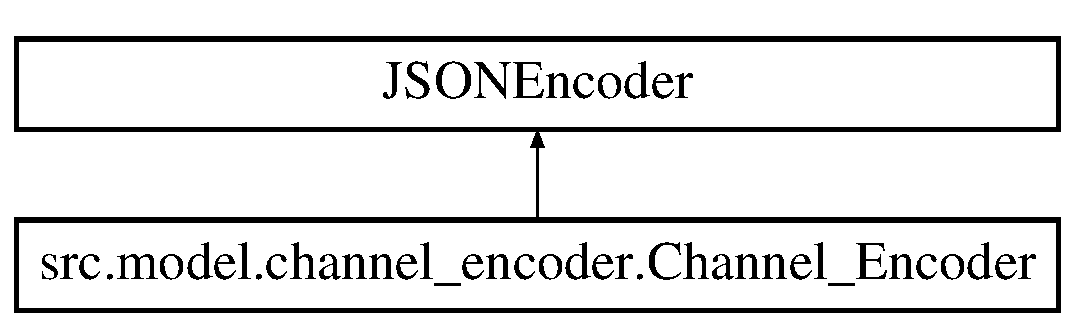
\includegraphics[height=2.000000cm]{classsrc_1_1model_1_1channel__encoder_1_1Channel__Encoder}
\end{center}
\end{figure}
\subsection*{Public Member Functions}
\begin{DoxyCompactItemize}
\item 
def \hyperlink{classsrc_1_1model_1_1channel__encoder_1_1Channel__Encoder_ab5eee724205efbd7ffd5f29b5547682a}{default} (self, obj)
\end{DoxyCompactItemize}


\subsection{Member Function Documentation}
\hypertarget{classsrc_1_1model_1_1channel__encoder_1_1Channel__Encoder_ab5eee724205efbd7ffd5f29b5547682a}{}\index{src\+::model\+::channel\+\_\+encoder\+::\+Channel\+\_\+\+Encoder@{src\+::model\+::channel\+\_\+encoder\+::\+Channel\+\_\+\+Encoder}!default@{default}}
\index{default@{default}!src\+::model\+::channel\+\_\+encoder\+::\+Channel\+\_\+\+Encoder@{src\+::model\+::channel\+\_\+encoder\+::\+Channel\+\_\+\+Encoder}}
\subsubsection[{default}]{\setlength{\rightskip}{0pt plus 5cm}def src.\+model.\+channel\+\_\+encoder.\+Channel\+\_\+\+Encoder.\+default (
\begin{DoxyParamCaption}
\item[{}]{self, }
\item[{}]{obj}
\end{DoxyParamCaption}
)}\label{classsrc_1_1model_1_1channel__encoder_1_1Channel__Encoder_ab5eee724205efbd7ffd5f29b5547682a}


The documentation for this class was generated from the following file\+:\begin{DoxyCompactItemize}
\item 
src/model/\hyperlink{channel__encoder_8py}{channel\+\_\+encoder.\+py}\end{DoxyCompactItemize}

\hypertarget{classsrc_1_1model_1_1channel__store_1_1Channel__Store}{}\section{src.\+model.\+channel\+\_\+store.\+Channel\+\_\+\+Store Class Reference}
\label{classsrc_1_1model_1_1channel__store_1_1Channel__Store}\index{src.\+model.\+channel\+\_\+store.\+Channel\+\_\+\+Store@{src.\+model.\+channel\+\_\+store.\+Channel\+\_\+\+Store}}
\subsection*{Public Member Functions}
\begin{DoxyCompactItemize}
\item 
def \hyperlink{classsrc_1_1model_1_1channel__store_1_1Channel__Store_adf1bcb70446bc48f0a6c7682666f3af7}{\+\_\+\+\_\+init\+\_\+\+\_\+} (self)
\item 
def \hyperlink{classsrc_1_1model_1_1channel__store_1_1Channel__Store_ab2cc111eceef9eb386ef89fec578e301}{get\+\_\+default} (self)
\item 
def \hyperlink{classsrc_1_1model_1_1channel__store_1_1Channel__Store_a83eb2469b676af82ffefcc30ab53e0a9}{append} (self, category)
\end{DoxyCompactItemize}
\subsection*{Public Attributes}
\begin{DoxyCompactItemize}
\item 
\hyperlink{classsrc_1_1model_1_1channel__store_1_1Channel__Store_a9e2372569f733406cb55b8c2610b0bf3}{categories}
\end{DoxyCompactItemize}
\subsection*{Static Public Attributes}
\begin{DoxyCompactItemize}
\item 
tuple \hyperlink{classsrc_1_1model_1_1channel__store_1_1Channel__Store_a3a896181a843b1c9be26a2d09d2af9c8}{A\+L\+L} = Category(\char`\"{}all\char`\"{})
\end{DoxyCompactItemize}
\subsection*{Private Member Functions}
\begin{DoxyCompactItemize}
\item 
def \hyperlink{classsrc_1_1model_1_1channel__store_1_1Channel__Store_af7273eaa7833915fe6dfac3d6f7c7222}{\+\_\+set\+\_\+default} (self, category)
\end{DoxyCompactItemize}


\subsection{Constructor \& Destructor Documentation}
\hypertarget{classsrc_1_1model_1_1channel__store_1_1Channel__Store_adf1bcb70446bc48f0a6c7682666f3af7}{}\index{src\+::model\+::channel\+\_\+store\+::\+Channel\+\_\+\+Store@{src\+::model\+::channel\+\_\+store\+::\+Channel\+\_\+\+Store}!\+\_\+\+\_\+init\+\_\+\+\_\+@{\+\_\+\+\_\+init\+\_\+\+\_\+}}
\index{\+\_\+\+\_\+init\+\_\+\+\_\+@{\+\_\+\+\_\+init\+\_\+\+\_\+}!src\+::model\+::channel\+\_\+store\+::\+Channel\+\_\+\+Store@{src\+::model\+::channel\+\_\+store\+::\+Channel\+\_\+\+Store}}
\subsubsection[{\+\_\+\+\_\+init\+\_\+\+\_\+}]{\setlength{\rightskip}{0pt plus 5cm}def src.\+model.\+channel\+\_\+store.\+Channel\+\_\+\+Store.\+\_\+\+\_\+init\+\_\+\+\_\+ (
\begin{DoxyParamCaption}
\item[{}]{self}
\end{DoxyParamCaption}
)}\label{classsrc_1_1model_1_1channel__store_1_1Channel__Store_adf1bcb70446bc48f0a6c7682666f3af7}


\subsection{Member Function Documentation}
\hypertarget{classsrc_1_1model_1_1channel__store_1_1Channel__Store_af7273eaa7833915fe6dfac3d6f7c7222}{}\index{src\+::model\+::channel\+\_\+store\+::\+Channel\+\_\+\+Store@{src\+::model\+::channel\+\_\+store\+::\+Channel\+\_\+\+Store}!\+\_\+set\+\_\+default@{\+\_\+set\+\_\+default}}
\index{\+\_\+set\+\_\+default@{\+\_\+set\+\_\+default}!src\+::model\+::channel\+\_\+store\+::\+Channel\+\_\+\+Store@{src\+::model\+::channel\+\_\+store\+::\+Channel\+\_\+\+Store}}
\subsubsection[{\+\_\+set\+\_\+default}]{\setlength{\rightskip}{0pt plus 5cm}def src.\+model.\+channel\+\_\+store.\+Channel\+\_\+\+Store.\+\_\+set\+\_\+default (
\begin{DoxyParamCaption}
\item[{}]{self, }
\item[{}]{category}
\end{DoxyParamCaption}
)\hspace{0.3cm}{\ttfamily [private]}}\label{classsrc_1_1model_1_1channel__store_1_1Channel__Store_af7273eaa7833915fe6dfac3d6f7c7222}
\hypertarget{classsrc_1_1model_1_1channel__store_1_1Channel__Store_a83eb2469b676af82ffefcc30ab53e0a9}{}\index{src\+::model\+::channel\+\_\+store\+::\+Channel\+\_\+\+Store@{src\+::model\+::channel\+\_\+store\+::\+Channel\+\_\+\+Store}!append@{append}}
\index{append@{append}!src\+::model\+::channel\+\_\+store\+::\+Channel\+\_\+\+Store@{src\+::model\+::channel\+\_\+store\+::\+Channel\+\_\+\+Store}}
\subsubsection[{append}]{\setlength{\rightskip}{0pt plus 5cm}def src.\+model.\+channel\+\_\+store.\+Channel\+\_\+\+Store.\+append (
\begin{DoxyParamCaption}
\item[{}]{self, }
\item[{}]{category}
\end{DoxyParamCaption}
)}\label{classsrc_1_1model_1_1channel__store_1_1Channel__Store_a83eb2469b676af82ffefcc30ab53e0a9}
\hypertarget{classsrc_1_1model_1_1channel__store_1_1Channel__Store_ab2cc111eceef9eb386ef89fec578e301}{}\index{src\+::model\+::channel\+\_\+store\+::\+Channel\+\_\+\+Store@{src\+::model\+::channel\+\_\+store\+::\+Channel\+\_\+\+Store}!get\+\_\+default@{get\+\_\+default}}
\index{get\+\_\+default@{get\+\_\+default}!src\+::model\+::channel\+\_\+store\+::\+Channel\+\_\+\+Store@{src\+::model\+::channel\+\_\+store\+::\+Channel\+\_\+\+Store}}
\subsubsection[{get\+\_\+default}]{\setlength{\rightskip}{0pt plus 5cm}def src.\+model.\+channel\+\_\+store.\+Channel\+\_\+\+Store.\+get\+\_\+default (
\begin{DoxyParamCaption}
\item[{}]{self}
\end{DoxyParamCaption}
)}\label{classsrc_1_1model_1_1channel__store_1_1Channel__Store_ab2cc111eceef9eb386ef89fec578e301}


\subsection{Member Data Documentation}
\hypertarget{classsrc_1_1model_1_1channel__store_1_1Channel__Store_a3a896181a843b1c9be26a2d09d2af9c8}{}\index{src\+::model\+::channel\+\_\+store\+::\+Channel\+\_\+\+Store@{src\+::model\+::channel\+\_\+store\+::\+Channel\+\_\+\+Store}!A\+L\+L@{A\+L\+L}}
\index{A\+L\+L@{A\+L\+L}!src\+::model\+::channel\+\_\+store\+::\+Channel\+\_\+\+Store@{src\+::model\+::channel\+\_\+store\+::\+Channel\+\_\+\+Store}}
\subsubsection[{A\+L\+L}]{\setlength{\rightskip}{0pt plus 5cm}tuple src.\+model.\+channel\+\_\+store.\+Channel\+\_\+\+Store.\+A\+L\+L = Category(\char`\"{}all\char`\"{})\hspace{0.3cm}{\ttfamily [static]}}\label{classsrc_1_1model_1_1channel__store_1_1Channel__Store_a3a896181a843b1c9be26a2d09d2af9c8}
\hypertarget{classsrc_1_1model_1_1channel__store_1_1Channel__Store_a9e2372569f733406cb55b8c2610b0bf3}{}\index{src\+::model\+::channel\+\_\+store\+::\+Channel\+\_\+\+Store@{src\+::model\+::channel\+\_\+store\+::\+Channel\+\_\+\+Store}!categories@{categories}}
\index{categories@{categories}!src\+::model\+::channel\+\_\+store\+::\+Channel\+\_\+\+Store@{src\+::model\+::channel\+\_\+store\+::\+Channel\+\_\+\+Store}}
\subsubsection[{categories}]{\setlength{\rightskip}{0pt plus 5cm}src.\+model.\+channel\+\_\+store.\+Channel\+\_\+\+Store.\+categories}\label{classsrc_1_1model_1_1channel__store_1_1Channel__Store_a9e2372569f733406cb55b8c2610b0bf3}


The documentation for this class was generated from the following file\+:\begin{DoxyCompactItemize}
\item 
src/model/\hyperlink{channel__store_8py}{channel\+\_\+store.\+py}\end{DoxyCompactItemize}

\hypertarget{classsrc_1_1core_1_1color_1_1Color}{}\section{src.\+core.\+color.\+Color Class Reference}
\label{classsrc_1_1core_1_1color_1_1Color}\index{src.\+core.\+color.\+Color@{src.\+core.\+color.\+Color}}
\subsection*{Static Public Attributes}
\begin{DoxyCompactItemize}
\item 
string \hyperlink{classsrc_1_1core_1_1color_1_1Color_ad9c1eb53da416b311597a25ec8b6fd52}{none} = \textquotesingle{}\textbackslash{}033\mbox{[}0m\textquotesingle{}
\item 
string \hyperlink{classsrc_1_1core_1_1color_1_1Color_a1031a20cc2bdf64cc3d28b2546cfcc4e}{red} = \textquotesingle{}\textbackslash{}033\mbox{[}91m\textquotesingle{}
\item 
string \hyperlink{classsrc_1_1core_1_1color_1_1Color_a90db613858d3ded1fa9fffa2970d6cac}{green} = \textquotesingle{}\textbackslash{}033\mbox{[}92m\textquotesingle{}
\item 
string \hyperlink{classsrc_1_1core_1_1color_1_1Color_ae679f19112a1c3c6c91b5e7b8bbe2571}{yellow} = \textquotesingle{}\textbackslash{}033\mbox{[}93m\textquotesingle{}
\item 
string \hyperlink{classsrc_1_1core_1_1color_1_1Color_ae551fbcf974c688355b334c6f4d7c411}{blue} = \textquotesingle{}\textbackslash{}033\mbox{[}94m\textquotesingle{}
\item 
string \hyperlink{classsrc_1_1core_1_1color_1_1Color_a7a5ac5a1852e67a22b6bdd2cf9640a74}{purple} = \textquotesingle{}\textbackslash{}033\mbox{[}95m\textquotesingle{}
\item 
string \hyperlink{classsrc_1_1core_1_1color_1_1Color_a4ff0ae2ff0959548a67750d4f2a10fad}{cyan} = \textquotesingle{}\textbackslash{}033\mbox{[}96m\textquotesingle{}
\item 
string \hyperlink{classsrc_1_1core_1_1color_1_1Color_a6b2f32d8cb5ac52330ea7633c4e8d7de}{white} = \textquotesingle{}\textbackslash{}033\mbox{[}97m\textquotesingle{}
\end{DoxyCompactItemize}


\subsection{Member Data Documentation}
\hypertarget{classsrc_1_1core_1_1color_1_1Color_ae551fbcf974c688355b334c6f4d7c411}{}\index{src\+::core\+::color\+::\+Color@{src\+::core\+::color\+::\+Color}!blue@{blue}}
\index{blue@{blue}!src\+::core\+::color\+::\+Color@{src\+::core\+::color\+::\+Color}}
\subsubsection[{blue}]{\setlength{\rightskip}{0pt plus 5cm}string src.\+core.\+color.\+Color.\+blue = \textquotesingle{}\textbackslash{}033\mbox{[}94m\textquotesingle{}\hspace{0.3cm}{\ttfamily [static]}}\label{classsrc_1_1core_1_1color_1_1Color_ae551fbcf974c688355b334c6f4d7c411}
\hypertarget{classsrc_1_1core_1_1color_1_1Color_a4ff0ae2ff0959548a67750d4f2a10fad}{}\index{src\+::core\+::color\+::\+Color@{src\+::core\+::color\+::\+Color}!cyan@{cyan}}
\index{cyan@{cyan}!src\+::core\+::color\+::\+Color@{src\+::core\+::color\+::\+Color}}
\subsubsection[{cyan}]{\setlength{\rightskip}{0pt plus 5cm}string src.\+core.\+color.\+Color.\+cyan = \textquotesingle{}\textbackslash{}033\mbox{[}96m\textquotesingle{}\hspace{0.3cm}{\ttfamily [static]}}\label{classsrc_1_1core_1_1color_1_1Color_a4ff0ae2ff0959548a67750d4f2a10fad}
\hypertarget{classsrc_1_1core_1_1color_1_1Color_a90db613858d3ded1fa9fffa2970d6cac}{}\index{src\+::core\+::color\+::\+Color@{src\+::core\+::color\+::\+Color}!green@{green}}
\index{green@{green}!src\+::core\+::color\+::\+Color@{src\+::core\+::color\+::\+Color}}
\subsubsection[{green}]{\setlength{\rightskip}{0pt plus 5cm}string src.\+core.\+color.\+Color.\+green = \textquotesingle{}\textbackslash{}033\mbox{[}92m\textquotesingle{}\hspace{0.3cm}{\ttfamily [static]}}\label{classsrc_1_1core_1_1color_1_1Color_a90db613858d3ded1fa9fffa2970d6cac}
\hypertarget{classsrc_1_1core_1_1color_1_1Color_ad9c1eb53da416b311597a25ec8b6fd52}{}\index{src\+::core\+::color\+::\+Color@{src\+::core\+::color\+::\+Color}!none@{none}}
\index{none@{none}!src\+::core\+::color\+::\+Color@{src\+::core\+::color\+::\+Color}}
\subsubsection[{none}]{\setlength{\rightskip}{0pt plus 5cm}string src.\+core.\+color.\+Color.\+none = \textquotesingle{}\textbackslash{}033\mbox{[}0m\textquotesingle{}\hspace{0.3cm}{\ttfamily [static]}}\label{classsrc_1_1core_1_1color_1_1Color_ad9c1eb53da416b311597a25ec8b6fd52}
\hypertarget{classsrc_1_1core_1_1color_1_1Color_a7a5ac5a1852e67a22b6bdd2cf9640a74}{}\index{src\+::core\+::color\+::\+Color@{src\+::core\+::color\+::\+Color}!purple@{purple}}
\index{purple@{purple}!src\+::core\+::color\+::\+Color@{src\+::core\+::color\+::\+Color}}
\subsubsection[{purple}]{\setlength{\rightskip}{0pt plus 5cm}string src.\+core.\+color.\+Color.\+purple = \textquotesingle{}\textbackslash{}033\mbox{[}95m\textquotesingle{}\hspace{0.3cm}{\ttfamily [static]}}\label{classsrc_1_1core_1_1color_1_1Color_a7a5ac5a1852e67a22b6bdd2cf9640a74}
\hypertarget{classsrc_1_1core_1_1color_1_1Color_a1031a20cc2bdf64cc3d28b2546cfcc4e}{}\index{src\+::core\+::color\+::\+Color@{src\+::core\+::color\+::\+Color}!red@{red}}
\index{red@{red}!src\+::core\+::color\+::\+Color@{src\+::core\+::color\+::\+Color}}
\subsubsection[{red}]{\setlength{\rightskip}{0pt plus 5cm}string src.\+core.\+color.\+Color.\+red = \textquotesingle{}\textbackslash{}033\mbox{[}91m\textquotesingle{}\hspace{0.3cm}{\ttfamily [static]}}\label{classsrc_1_1core_1_1color_1_1Color_a1031a20cc2bdf64cc3d28b2546cfcc4e}
\hypertarget{classsrc_1_1core_1_1color_1_1Color_a6b2f32d8cb5ac52330ea7633c4e8d7de}{}\index{src\+::core\+::color\+::\+Color@{src\+::core\+::color\+::\+Color}!white@{white}}
\index{white@{white}!src\+::core\+::color\+::\+Color@{src\+::core\+::color\+::\+Color}}
\subsubsection[{white}]{\setlength{\rightskip}{0pt plus 5cm}string src.\+core.\+color.\+Color.\+white = \textquotesingle{}\textbackslash{}033\mbox{[}97m\textquotesingle{}\hspace{0.3cm}{\ttfamily [static]}}\label{classsrc_1_1core_1_1color_1_1Color_a6b2f32d8cb5ac52330ea7633c4e8d7de}
\hypertarget{classsrc_1_1core_1_1color_1_1Color_ae679f19112a1c3c6c91b5e7b8bbe2571}{}\index{src\+::core\+::color\+::\+Color@{src\+::core\+::color\+::\+Color}!yellow@{yellow}}
\index{yellow@{yellow}!src\+::core\+::color\+::\+Color@{src\+::core\+::color\+::\+Color}}
\subsubsection[{yellow}]{\setlength{\rightskip}{0pt plus 5cm}string src.\+core.\+color.\+Color.\+yellow = \textquotesingle{}\textbackslash{}033\mbox{[}93m\textquotesingle{}\hspace{0.3cm}{\ttfamily [static]}}\label{classsrc_1_1core_1_1color_1_1Color_ae679f19112a1c3c6c91b5e7b8bbe2571}


The documentation for this class was generated from the following file\+:\begin{DoxyCompactItemize}
\item 
src/core/\hyperlink{color_8py}{color.\+py}\end{DoxyCompactItemize}

\hypertarget{classtest__UDP_1_1Destination}{}\section{test\+\_\+\+U\+D\+P.\+Destination Class Reference}
\label{classtest__UDP_1_1Destination}\index{test\+\_\+\+U\+D\+P.\+Destination@{test\+\_\+\+U\+D\+P.\+Destination}}
\subsection*{Public Member Functions}
\begin{DoxyCompactItemize}
\item 
def \hyperlink{classtest__UDP_1_1Destination_a5cbe45be64d823adde03d72ca523a3f2}{get} (self)
\end{DoxyCompactItemize}
\subsection*{Static Public Attributes}
\begin{DoxyCompactItemize}
\item 
string \hyperlink{classtest__UDP_1_1Destination_ac5fb7c516eb489d012703f654075ebe2}{addr} = \char`\"{}150.\+214.\+150.\+68\char`\"{}
\item 
int \hyperlink{classtest__UDP_1_1Destination_a1d6099bcb62697225cfacab6e7db3fc9}{port} = 4551
\end{DoxyCompactItemize}


\subsection{Member Function Documentation}
\hypertarget{classtest__UDP_1_1Destination_a5cbe45be64d823adde03d72ca523a3f2}{}\index{test\+\_\+\+U\+D\+P\+::\+Destination@{test\+\_\+\+U\+D\+P\+::\+Destination}!get@{get}}
\index{get@{get}!test\+\_\+\+U\+D\+P\+::\+Destination@{test\+\_\+\+U\+D\+P\+::\+Destination}}
\subsubsection[{get}]{\setlength{\rightskip}{0pt plus 5cm}def test\+\_\+\+U\+D\+P.\+Destination.\+get (
\begin{DoxyParamCaption}
\item[{}]{self}
\end{DoxyParamCaption}
)}\label{classtest__UDP_1_1Destination_a5cbe45be64d823adde03d72ca523a3f2}


\subsection{Member Data Documentation}
\hypertarget{classtest__UDP_1_1Destination_ac5fb7c516eb489d012703f654075ebe2}{}\index{test\+\_\+\+U\+D\+P\+::\+Destination@{test\+\_\+\+U\+D\+P\+::\+Destination}!addr@{addr}}
\index{addr@{addr}!test\+\_\+\+U\+D\+P\+::\+Destination@{test\+\_\+\+U\+D\+P\+::\+Destination}}
\subsubsection[{addr}]{\setlength{\rightskip}{0pt plus 5cm}string test\+\_\+\+U\+D\+P.\+Destination.\+addr = \char`\"{}150.\+214.\+150.\+68\char`\"{}\hspace{0.3cm}{\ttfamily [static]}}\label{classtest__UDP_1_1Destination_ac5fb7c516eb489d012703f654075ebe2}
\hypertarget{classtest__UDP_1_1Destination_a1d6099bcb62697225cfacab6e7db3fc9}{}\index{test\+\_\+\+U\+D\+P\+::\+Destination@{test\+\_\+\+U\+D\+P\+::\+Destination}!port@{port}}
\index{port@{port}!test\+\_\+\+U\+D\+P\+::\+Destination@{test\+\_\+\+U\+D\+P\+::\+Destination}}
\subsubsection[{port}]{\setlength{\rightskip}{0pt plus 5cm}int test\+\_\+\+U\+D\+P.\+Destination.\+port = 4551\hspace{0.3cm}{\ttfamily [static]}}\label{classtest__UDP_1_1Destination_a1d6099bcb62697225cfacab6e7db3fc9}


The documentation for this class was generated from the following file\+:\begin{DoxyCompactItemize}
\item 
tools/\hyperlink{test__UDP_8py}{test\+\_\+\+U\+D\+P.\+py}\end{DoxyCompactItemize}

\hypertarget{classsrc_1_1lib_1_1vlc_1_1Event}{}\section{src.\+lib.\+vlc.\+Event Class Reference}
\label{classsrc_1_1lib_1_1vlc_1_1Event}\index{src.\+lib.\+vlc.\+Event@{src.\+lib.\+vlc.\+Event}}
Inheritance diagram for src.\+lib.\+vlc.\+Event\+:\begin{figure}[H]
\begin{center}
\leavevmode
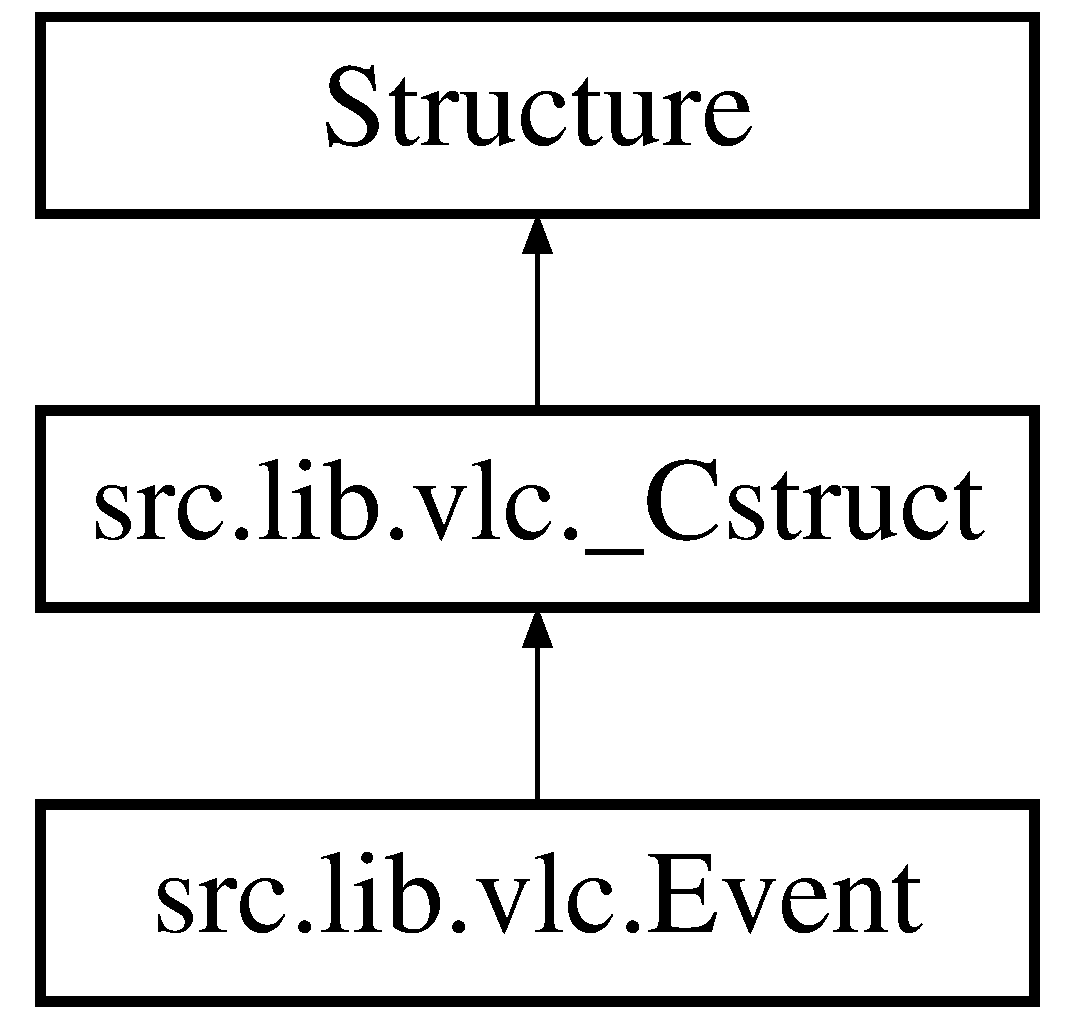
\includegraphics[height=3.000000cm]{classsrc_1_1lib_1_1vlc_1_1Event}
\end{center}
\end{figure}
\subsection*{Static Private Attributes}
\begin{DoxyCompactItemize}
\item 
list \hyperlink{classsrc_1_1lib_1_1vlc_1_1Event_aa96b52e8350c1c283c290cf719e6b417}{\+\_\+fields\+\_\+}
\end{DoxyCompactItemize}
\subsection*{Additional Inherited Members}


\subsection{Member Data Documentation}
\hypertarget{classsrc_1_1lib_1_1vlc_1_1Event_aa96b52e8350c1c283c290cf719e6b417}{}\index{src\+::lib\+::vlc\+::\+Event@{src\+::lib\+::vlc\+::\+Event}!\+\_\+fields\+\_\+@{\+\_\+fields\+\_\+}}
\index{\+\_\+fields\+\_\+@{\+\_\+fields\+\_\+}!src\+::lib\+::vlc\+::\+Event@{src\+::lib\+::vlc\+::\+Event}}
\subsubsection[{\+\_\+fields\+\_\+}]{\setlength{\rightskip}{0pt plus 5cm}list src.\+lib.\+vlc.\+Event.\+\_\+fields\+\_\+\hspace{0.3cm}{\ttfamily [static]}, {\ttfamily [private]}}\label{classsrc_1_1lib_1_1vlc_1_1Event_aa96b52e8350c1c283c290cf719e6b417}
{\bfseries Initial value\+:}
\begin{DoxyCode}
1 = [
2         (\textcolor{stringliteral}{'type'},   EventType      ),
3         (\textcolor{stringliteral}{'object'}, ctypes.c\_void\_p),
4         (\textcolor{stringliteral}{'}\textcolor{stringliteral}{u',      EventUnion     ),}
5 \textcolor{stringliteral}{    ]}
\end{DoxyCode}


The documentation for this class was generated from the following file\+:\begin{DoxyCompactItemize}
\item 
src/lib/\hyperlink{vlc_8py}{vlc.\+py}\end{DoxyCompactItemize}

\hypertarget{classsrc_1_1lib_1_1vlc_1_1EventManager}{}\section{src.\+lib.\+vlc.\+Event\+Manager Class Reference}
\label{classsrc_1_1lib_1_1vlc_1_1EventManager}\index{src.\+lib.\+vlc.\+Event\+Manager@{src.\+lib.\+vlc.\+Event\+Manager}}
Inheritance diagram for src.\+lib.\+vlc.\+Event\+Manager\+:\begin{figure}[H]
\begin{center}
\leavevmode
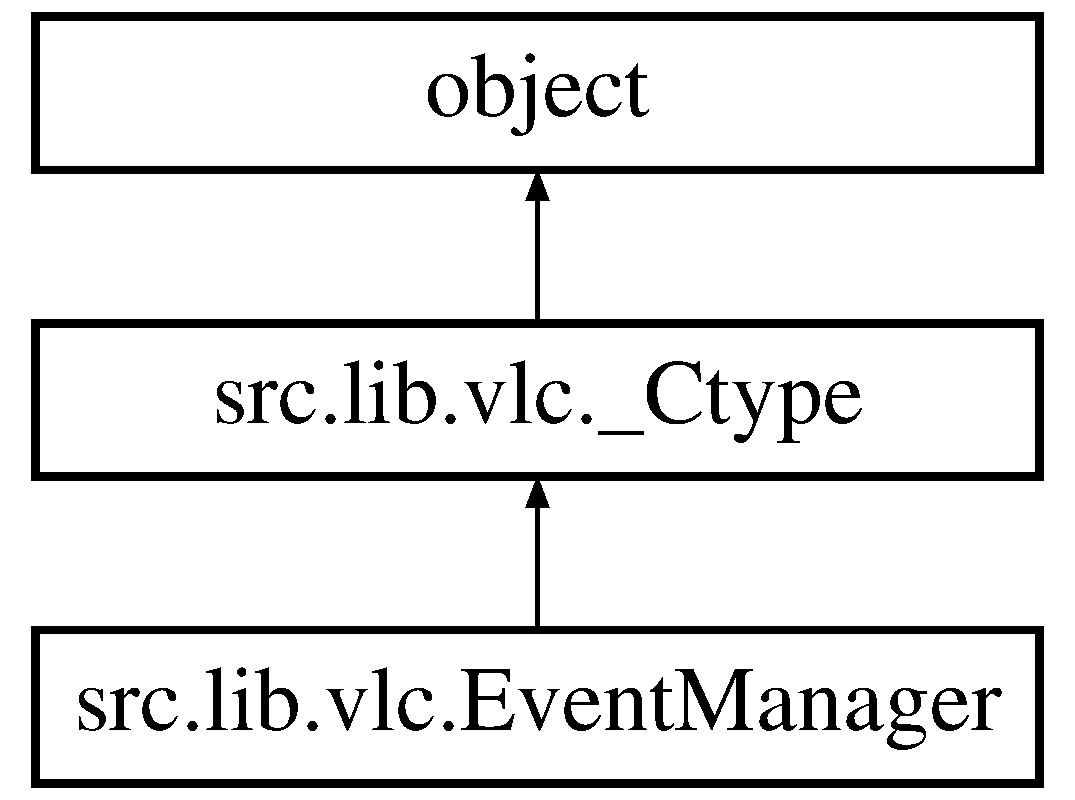
\includegraphics[height=3.000000cm]{classsrc_1_1lib_1_1vlc_1_1EventManager}
\end{center}
\end{figure}
\subsection*{Public Member Functions}
\begin{DoxyCompactItemize}
\item 
def \hyperlink{classsrc_1_1lib_1_1vlc_1_1EventManager_a29af220e01df1ed851e47e814f510ae8}{\+\_\+\+\_\+new\+\_\+\+\_\+}
\item 
def \hyperlink{classsrc_1_1lib_1_1vlc_1_1EventManager_a1f9f75744696ef79235485c25243d967}{event\+\_\+attach} (self, eventtype, callback, args, kwds)
\item 
def \hyperlink{classsrc_1_1lib_1_1vlc_1_1EventManager_ade3c764c0bf826d28c3845e94c1ee1c5}{event\+\_\+detach} (self, eventtype)
\end{DoxyCompactItemize}
\subsection*{Private Attributes}
\begin{DoxyCompactItemize}
\item 
\hyperlink{classsrc_1_1lib_1_1vlc_1_1EventManager_a50815d3eaa5da503c6a966ab9f2acce1}{\+\_\+callbacks}
\end{DoxyCompactItemize}
\subsection*{Static Private Attributes}
\begin{DoxyCompactItemize}
\item 
\hyperlink{classsrc_1_1lib_1_1vlc_1_1EventManager_ad477af10daa2903a52bc0f142fca198d}{\+\_\+callback\+\_\+handler} = None
\item 
dictionary \hyperlink{classsrc_1_1lib_1_1vlc_1_1EventManager_a3cbe5bf81d4bf18946cf50aa1383766c}{\+\_\+callbacks} = \{\}
\end{DoxyCompactItemize}
\subsection*{Additional Inherited Members}


\subsection{Detailed Description}
\begin{DoxyVerb}Create an event manager with callback handler.

This class interposes the registration and handling of
event notifications in order to (a) remove the need for
decorating each callback functions with the decorator
'@callbackmethod', (b) allow any number of positional
and/or keyword arguments to the callback (in addition
to the Event instance) and (c) to preserve the Python
objects such that the callback and argument objects
remain alive (i.e. are not garbage collected) until
B{after} the notification has been unregistered.

@note: Only a single notification can be registered
for each event type in an EventManager instance.\end{DoxyVerb}
 

\subsection{Member Function Documentation}
\hypertarget{classsrc_1_1lib_1_1vlc_1_1EventManager_a29af220e01df1ed851e47e814f510ae8}{}\index{src\+::lib\+::vlc\+::\+Event\+Manager@{src\+::lib\+::vlc\+::\+Event\+Manager}!\+\_\+\+\_\+new\+\_\+\+\_\+@{\+\_\+\+\_\+new\+\_\+\+\_\+}}
\index{\+\_\+\+\_\+new\+\_\+\+\_\+@{\+\_\+\+\_\+new\+\_\+\+\_\+}!src\+::lib\+::vlc\+::\+Event\+Manager@{src\+::lib\+::vlc\+::\+Event\+Manager}}
\subsubsection[{\+\_\+\+\_\+new\+\_\+\+\_\+}]{\setlength{\rightskip}{0pt plus 5cm}def src.\+lib.\+vlc.\+Event\+Manager.\+\_\+\+\_\+new\+\_\+\+\_\+ (
\begin{DoxyParamCaption}
\item[{}]{cls, }
\item[{}]{ptr = {\ttfamily {\bf \+\_\+internal\+\_\+guard}}}
\end{DoxyParamCaption}
)}\label{classsrc_1_1lib_1_1vlc_1_1EventManager_a29af220e01df1ed851e47e814f510ae8}
\hypertarget{classsrc_1_1lib_1_1vlc_1_1EventManager_a1f9f75744696ef79235485c25243d967}{}\index{src\+::lib\+::vlc\+::\+Event\+Manager@{src\+::lib\+::vlc\+::\+Event\+Manager}!event\+\_\+attach@{event\+\_\+attach}}
\index{event\+\_\+attach@{event\+\_\+attach}!src\+::lib\+::vlc\+::\+Event\+Manager@{src\+::lib\+::vlc\+::\+Event\+Manager}}
\subsubsection[{event\+\_\+attach}]{\setlength{\rightskip}{0pt plus 5cm}def src.\+lib.\+vlc.\+Event\+Manager.\+event\+\_\+attach (
\begin{DoxyParamCaption}
\item[{}]{self, }
\item[{}]{eventtype, }
\item[{}]{callback, }
\item[{}]{args, }
\item[{}]{kwds}
\end{DoxyParamCaption}
)}\label{classsrc_1_1lib_1_1vlc_1_1EventManager_a1f9f75744696ef79235485c25243d967}
\begin{DoxyVerb}Register an event notification.

@param eventtype: the desired event type to be notified about.
@param callback: the function to call when the event occurs.
@param args: optional positional arguments for the callback.
@param kwds: optional keyword arguments for the callback.
@return: 0 on success, ENOMEM on error.

@note: The callback function must have at least one argument,
an Event instance.  Any other, optional positional and keyword
arguments are in B{addition} to the first one.
\end{DoxyVerb}
 \hypertarget{classsrc_1_1lib_1_1vlc_1_1EventManager_ade3c764c0bf826d28c3845e94c1ee1c5}{}\index{src\+::lib\+::vlc\+::\+Event\+Manager@{src\+::lib\+::vlc\+::\+Event\+Manager}!event\+\_\+detach@{event\+\_\+detach}}
\index{event\+\_\+detach@{event\+\_\+detach}!src\+::lib\+::vlc\+::\+Event\+Manager@{src\+::lib\+::vlc\+::\+Event\+Manager}}
\subsubsection[{event\+\_\+detach}]{\setlength{\rightskip}{0pt plus 5cm}def src.\+lib.\+vlc.\+Event\+Manager.\+event\+\_\+detach (
\begin{DoxyParamCaption}
\item[{}]{self, }
\item[{}]{eventtype}
\end{DoxyParamCaption}
)}\label{classsrc_1_1lib_1_1vlc_1_1EventManager_ade3c764c0bf826d28c3845e94c1ee1c5}
\begin{DoxyVerb}Unregister an event notification.

@param eventtype: the event type notification to be removed.
\end{DoxyVerb}
 

\subsection{Member Data Documentation}
\hypertarget{classsrc_1_1lib_1_1vlc_1_1EventManager_ad477af10daa2903a52bc0f142fca198d}{}\index{src\+::lib\+::vlc\+::\+Event\+Manager@{src\+::lib\+::vlc\+::\+Event\+Manager}!\+\_\+callback\+\_\+handler@{\+\_\+callback\+\_\+handler}}
\index{\+\_\+callback\+\_\+handler@{\+\_\+callback\+\_\+handler}!src\+::lib\+::vlc\+::\+Event\+Manager@{src\+::lib\+::vlc\+::\+Event\+Manager}}
\subsubsection[{\+\_\+callback\+\_\+handler}]{\setlength{\rightskip}{0pt plus 5cm}src.\+lib.\+vlc.\+Event\+Manager.\+\_\+callback\+\_\+handler = None\hspace{0.3cm}{\ttfamily [static]}, {\ttfamily [private]}}\label{classsrc_1_1lib_1_1vlc_1_1EventManager_ad477af10daa2903a52bc0f142fca198d}
\hypertarget{classsrc_1_1lib_1_1vlc_1_1EventManager_a3cbe5bf81d4bf18946cf50aa1383766c}{}\index{src\+::lib\+::vlc\+::\+Event\+Manager@{src\+::lib\+::vlc\+::\+Event\+Manager}!\+\_\+callbacks@{\+\_\+callbacks}}
\index{\+\_\+callbacks@{\+\_\+callbacks}!src\+::lib\+::vlc\+::\+Event\+Manager@{src\+::lib\+::vlc\+::\+Event\+Manager}}
\subsubsection[{\+\_\+callbacks}]{\setlength{\rightskip}{0pt plus 5cm}dictionary src.\+lib.\+vlc.\+Event\+Manager.\+\_\+callbacks = \{\}\hspace{0.3cm}{\ttfamily [static]}, {\ttfamily [private]}}\label{classsrc_1_1lib_1_1vlc_1_1EventManager_a3cbe5bf81d4bf18946cf50aa1383766c}
\hypertarget{classsrc_1_1lib_1_1vlc_1_1EventManager_a50815d3eaa5da503c6a966ab9f2acce1}{}\index{src\+::lib\+::vlc\+::\+Event\+Manager@{src\+::lib\+::vlc\+::\+Event\+Manager}!\+\_\+callbacks@{\+\_\+callbacks}}
\index{\+\_\+callbacks@{\+\_\+callbacks}!src\+::lib\+::vlc\+::\+Event\+Manager@{src\+::lib\+::vlc\+::\+Event\+Manager}}
\subsubsection[{\+\_\+callbacks}]{\setlength{\rightskip}{0pt plus 5cm}src.\+lib.\+vlc.\+Event\+Manager.\+\_\+callbacks\hspace{0.3cm}{\ttfamily [private]}}\label{classsrc_1_1lib_1_1vlc_1_1EventManager_a50815d3eaa5da503c6a966ab9f2acce1}


The documentation for this class was generated from the following file\+:\begin{DoxyCompactItemize}
\item 
src/lib/\hyperlink{vlc_8py}{vlc.\+py}\end{DoxyCompactItemize}

\hypertarget{classsrc_1_1lib_1_1vlc_1_1EventType}{}\section{src.\+lib.\+vlc.\+Event\+Type Class Reference}
\label{classsrc_1_1lib_1_1vlc_1_1EventType}\index{src.\+lib.\+vlc.\+Event\+Type@{src.\+lib.\+vlc.\+Event\+Type}}
Inheritance diagram for src.\+lib.\+vlc.\+Event\+Type\+:\begin{figure}[H]
\begin{center}
\leavevmode
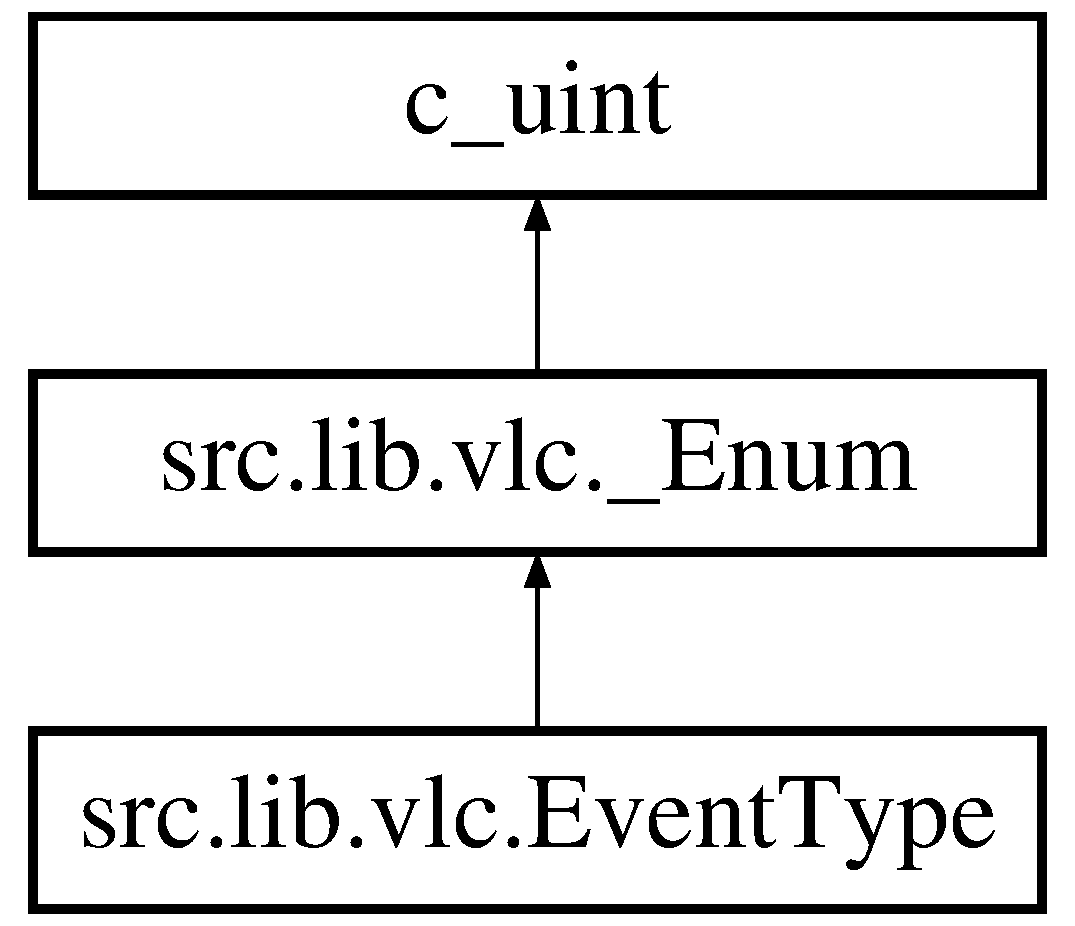
\includegraphics[height=3.000000cm]{classsrc_1_1lib_1_1vlc_1_1EventType}
\end{center}
\end{figure}
\subsection*{Static Private Attributes}
\begin{DoxyCompactItemize}
\item 
dictionary \hyperlink{classsrc_1_1lib_1_1vlc_1_1EventType_a91ba07bdc81b31c96003ce137c162764}{\+\_\+enum\+\_\+names\+\_\+}
\end{DoxyCompactItemize}
\subsection*{Additional Inherited Members}


\subsection{Detailed Description}
\begin{DoxyVerb}Event types.
\end{DoxyVerb}
 

\subsection{Member Data Documentation}
\hypertarget{classsrc_1_1lib_1_1vlc_1_1EventType_a91ba07bdc81b31c96003ce137c162764}{}\index{src\+::lib\+::vlc\+::\+Event\+Type@{src\+::lib\+::vlc\+::\+Event\+Type}!\+\_\+enum\+\_\+names\+\_\+@{\+\_\+enum\+\_\+names\+\_\+}}
\index{\+\_\+enum\+\_\+names\+\_\+@{\+\_\+enum\+\_\+names\+\_\+}!src\+::lib\+::vlc\+::\+Event\+Type@{src\+::lib\+::vlc\+::\+Event\+Type}}
\subsubsection[{\+\_\+enum\+\_\+names\+\_\+}]{\setlength{\rightskip}{0pt plus 5cm}dictionary src.\+lib.\+vlc.\+Event\+Type.\+\_\+enum\+\_\+names\+\_\+\hspace{0.3cm}{\ttfamily [static]}, {\ttfamily [private]}}\label{classsrc_1_1lib_1_1vlc_1_1EventType_a91ba07bdc81b31c96003ce137c162764}


The documentation for this class was generated from the following file\+:\begin{DoxyCompactItemize}
\item 
src/lib/\hyperlink{vlc_8py}{vlc.\+py}\end{DoxyCompactItemize}

\hypertarget{classsrc_1_1lib_1_1vlc_1_1EventUnion}{}\section{src.\+lib.\+vlc.\+Event\+Union Class Reference}
\label{classsrc_1_1lib_1_1vlc_1_1EventUnion}\index{src.\+lib.\+vlc.\+Event\+Union@{src.\+lib.\+vlc.\+Event\+Union}}
Inheritance diagram for src.\+lib.\+vlc.\+Event\+Union\+:\begin{figure}[H]
\begin{center}
\leavevmode
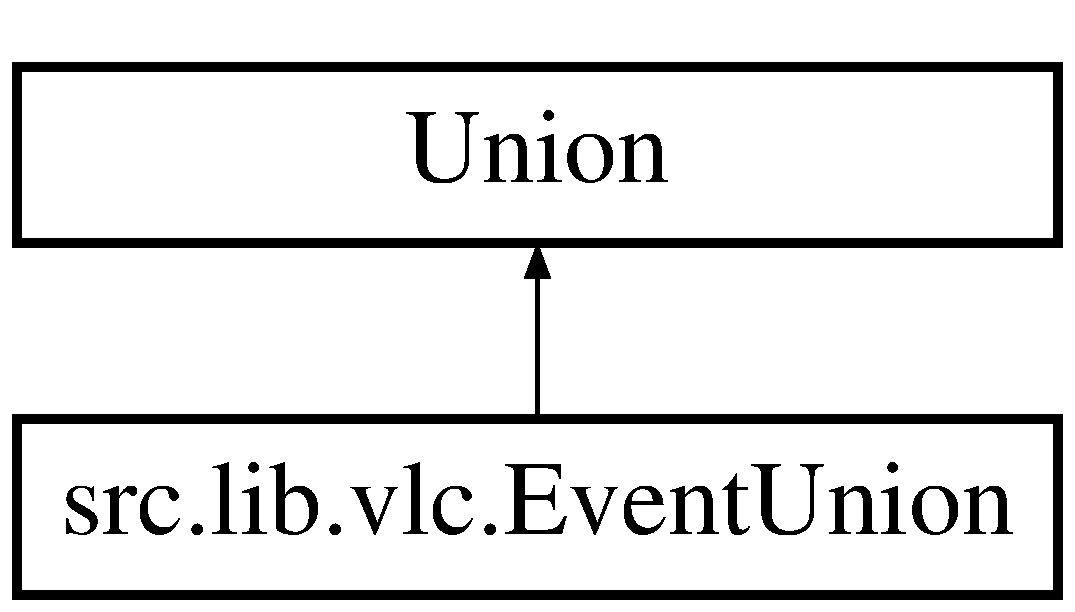
\includegraphics[height=2.000000cm]{classsrc_1_1lib_1_1vlc_1_1EventUnion}
\end{center}
\end{figure}
\subsection*{Static Private Attributes}
\begin{DoxyCompactItemize}
\item 
list \hyperlink{classsrc_1_1lib_1_1vlc_1_1EventUnion_aadde1d5693ac89f6f6e3169a33481ef6}{\+\_\+fields\+\_\+}
\end{DoxyCompactItemize}


\subsection{Member Data Documentation}
\hypertarget{classsrc_1_1lib_1_1vlc_1_1EventUnion_aadde1d5693ac89f6f6e3169a33481ef6}{}\index{src\+::lib\+::vlc\+::\+Event\+Union@{src\+::lib\+::vlc\+::\+Event\+Union}!\+\_\+fields\+\_\+@{\+\_\+fields\+\_\+}}
\index{\+\_\+fields\+\_\+@{\+\_\+fields\+\_\+}!src\+::lib\+::vlc\+::\+Event\+Union@{src\+::lib\+::vlc\+::\+Event\+Union}}
\subsubsection[{\+\_\+fields\+\_\+}]{\setlength{\rightskip}{0pt plus 5cm}list src.\+lib.\+vlc.\+Event\+Union.\+\_\+fields\+\_\+\hspace{0.3cm}{\ttfamily [static]}, {\ttfamily [private]}}\label{classsrc_1_1lib_1_1vlc_1_1EventUnion_aadde1d5693ac89f6f6e3169a33481ef6}
{\bfseries Initial value\+:}
\begin{DoxyCode}
1 = [
2         (\textcolor{stringliteral}{'meta\_type'},    ctypes.c\_uint    ),
3         (\textcolor{stringliteral}{'new\_child'},    ctypes.c\_uint    ),
4         (\textcolor{stringliteral}{'new\_duration'}, ctypes.c\_longlong),
5         (\textcolor{stringliteral}{'new\_status'},   ctypes.c\_int     ),
6         (\textcolor{stringliteral}{'media'},        ctypes.c\_void\_p  ),
7         (\textcolor{stringliteral}{'new\_state'},    ctypes.c\_uint    ),
8         \textcolor{comment}{# Media instance}
9         (\textcolor{stringliteral}{'new\_position'}, ctypes.c\_float   ),
10         (\textcolor{stringliteral}{'new\_time'},     ctypes.c\_longlong),
11         (\textcolor{stringliteral}{'new\_title'},    ctypes.c\_int     ),
12         (\textcolor{stringliteral}{'new\_seekable'}, ctypes.c\_longlong),
13         (\textcolor{stringliteral}{'new\_pausable'}, ctypes.c\_longlong),
14         \textcolor{comment}{# FIXME: Skipped MediaList and MediaListView...}
15         (\textcolor{stringliteral}{'filename'},     ctypes.c\_char\_p  ),
16         (\textcolor{stringliteral}{'new\_length'},   ctypes.c\_longlong),
17         (\textcolor{stringliteral}{'media\_event'},  MediaEvent       ),
18     ]
\end{DoxyCode}


The documentation for this class was generated from the following file\+:\begin{DoxyCompactItemize}
\item 
src/lib/\hyperlink{vlc_8py}{vlc.\+py}\end{DoxyCompactItemize}

\hypertarget{classsrc_1_1view_1_1export__box_1_1Export__Box}{}\section{src.\+view.\+export\+\_\+box.\+Export\+\_\+\+Box Class Reference}
\label{classsrc_1_1view_1_1export__box_1_1Export__Box}\index{src.\+view.\+export\+\_\+box.\+Export\+\_\+\+Box@{src.\+view.\+export\+\_\+box.\+Export\+\_\+\+Box}}
\subsection*{Public Member Functions}
\begin{DoxyCompactItemize}
\item 
def \hyperlink{classsrc_1_1view_1_1export__box_1_1Export__Box_ada19335761501a6d4f434146ecc97158}{\+\_\+\+\_\+init\+\_\+\+\_\+} (self)
\item 
def \hyperlink{classsrc_1_1view_1_1export__box_1_1Export__Box_ac333f6fdd40bf2349b9780333d983cbd}{load\+\_\+widgets} (self)
\item 
def \hyperlink{classsrc_1_1view_1_1export__box_1_1Export__Box_a2158ef4ddbc92c315bac9c9f065ddd07}{add\+\_\+channel\+\_\+list\+\_\+column} (self, title, column\+Id)
\item 
def \hyperlink{classsrc_1_1view_1_1export__box_1_1Export__Box_ac45a8c69e4e5e425f966ad07bcf31c52}{create\+\_\+list\+\_\+view} (self)
\end{DoxyCompactItemize}
\subsection*{Public Attributes}
\begin{DoxyCompactItemize}
\item 
\hyperlink{classsrc_1_1view_1_1export__box_1_1Export__Box_a04e81aa445620822397953c0fa3276f8}{interface}
\item 
\hyperlink{classsrc_1_1view_1_1export__box_1_1Export__Box_a9914ddf2315d31a118cd2f09f65f4ce9}{list\+\_\+store}
\item 
\hyperlink{classsrc_1_1view_1_1export__box_1_1Export__Box_aaa8b2ffcbcfbfb4a35e071da47409f3b}{export\+\_\+box}
\item 
\hyperlink{classsrc_1_1view_1_1export__box_1_1Export__Box_a8592732aeaa91ca10fe5dda340981259}{listview}
\item 
\hyperlink{classsrc_1_1view_1_1export__box_1_1Export__Box_aa98bee95ddcf1a265e3c90c4398fb79b}{export\+\_\+button}
\item 
\hyperlink{classsrc_1_1view_1_1export__box_1_1Export__Box_a999e9883f63f4f34312015b01cd0e28f}{cancel\+\_\+button}
\item 
\hyperlink{classsrc_1_1view_1_1export__box_1_1Export__Box_a94d8549aa604bd891b9f5de86f5a6f3e}{text\+\_\+entry}
\item 
\hyperlink{classsrc_1_1view_1_1export__box_1_1Export__Box_adb064561924b8f67b4537161d584401b}{column\+\_\+string}
\end{DoxyCompactItemize}


\subsection{Constructor \& Destructor Documentation}
\hypertarget{classsrc_1_1view_1_1export__box_1_1Export__Box_ada19335761501a6d4f434146ecc97158}{}\index{src\+::view\+::export\+\_\+box\+::\+Export\+\_\+\+Box@{src\+::view\+::export\+\_\+box\+::\+Export\+\_\+\+Box}!\+\_\+\+\_\+init\+\_\+\+\_\+@{\+\_\+\+\_\+init\+\_\+\+\_\+}}
\index{\+\_\+\+\_\+init\+\_\+\+\_\+@{\+\_\+\+\_\+init\+\_\+\+\_\+}!src\+::view\+::export\+\_\+box\+::\+Export\+\_\+\+Box@{src\+::view\+::export\+\_\+box\+::\+Export\+\_\+\+Box}}
\subsubsection[{\+\_\+\+\_\+init\+\_\+\+\_\+}]{\setlength{\rightskip}{0pt plus 5cm}def src.\+view.\+export\+\_\+box.\+Export\+\_\+\+Box.\+\_\+\+\_\+init\+\_\+\+\_\+ (
\begin{DoxyParamCaption}
\item[{}]{self}
\end{DoxyParamCaption}
)}\label{classsrc_1_1view_1_1export__box_1_1Export__Box_ada19335761501a6d4f434146ecc97158}


\subsection{Member Function Documentation}
\hypertarget{classsrc_1_1view_1_1export__box_1_1Export__Box_a2158ef4ddbc92c315bac9c9f065ddd07}{}\index{src\+::view\+::export\+\_\+box\+::\+Export\+\_\+\+Box@{src\+::view\+::export\+\_\+box\+::\+Export\+\_\+\+Box}!add\+\_\+channel\+\_\+list\+\_\+column@{add\+\_\+channel\+\_\+list\+\_\+column}}
\index{add\+\_\+channel\+\_\+list\+\_\+column@{add\+\_\+channel\+\_\+list\+\_\+column}!src\+::view\+::export\+\_\+box\+::\+Export\+\_\+\+Box@{src\+::view\+::export\+\_\+box\+::\+Export\+\_\+\+Box}}
\subsubsection[{add\+\_\+channel\+\_\+list\+\_\+column}]{\setlength{\rightskip}{0pt plus 5cm}def src.\+view.\+export\+\_\+box.\+Export\+\_\+\+Box.\+add\+\_\+channel\+\_\+list\+\_\+column (
\begin{DoxyParamCaption}
\item[{}]{self, }
\item[{}]{title, }
\item[{}]{column\+Id}
\end{DoxyParamCaption}
)}\label{classsrc_1_1view_1_1export__box_1_1Export__Box_a2158ef4ddbc92c315bac9c9f065ddd07}
\begin{DoxyVerb}This function adds a column to the list view.
First it create the Gtk.TreeViewColumn and then set
some needed properties\end{DoxyVerb}
 \hypertarget{classsrc_1_1view_1_1export__box_1_1Export__Box_ac45a8c69e4e5e425f966ad07bcf31c52}{}\index{src\+::view\+::export\+\_\+box\+::\+Export\+\_\+\+Box@{src\+::view\+::export\+\_\+box\+::\+Export\+\_\+\+Box}!create\+\_\+list\+\_\+view@{create\+\_\+list\+\_\+view}}
\index{create\+\_\+list\+\_\+view@{create\+\_\+list\+\_\+view}!src\+::view\+::export\+\_\+box\+::\+Export\+\_\+\+Box@{src\+::view\+::export\+\_\+box\+::\+Export\+\_\+\+Box}}
\subsubsection[{create\+\_\+list\+\_\+view}]{\setlength{\rightskip}{0pt plus 5cm}def src.\+view.\+export\+\_\+box.\+Export\+\_\+\+Box.\+create\+\_\+list\+\_\+view (
\begin{DoxyParamCaption}
\item[{}]{self}
\end{DoxyParamCaption}
)}\label{classsrc_1_1view_1_1export__box_1_1Export__Box_ac45a8c69e4e5e425f966ad07bcf31c52}
\hypertarget{classsrc_1_1view_1_1export__box_1_1Export__Box_ac333f6fdd40bf2349b9780333d983cbd}{}\index{src\+::view\+::export\+\_\+box\+::\+Export\+\_\+\+Box@{src\+::view\+::export\+\_\+box\+::\+Export\+\_\+\+Box}!load\+\_\+widgets@{load\+\_\+widgets}}
\index{load\+\_\+widgets@{load\+\_\+widgets}!src\+::view\+::export\+\_\+box\+::\+Export\+\_\+\+Box@{src\+::view\+::export\+\_\+box\+::\+Export\+\_\+\+Box}}
\subsubsection[{load\+\_\+widgets}]{\setlength{\rightskip}{0pt plus 5cm}def src.\+view.\+export\+\_\+box.\+Export\+\_\+\+Box.\+load\+\_\+widgets (
\begin{DoxyParamCaption}
\item[{}]{self}
\end{DoxyParamCaption}
)}\label{classsrc_1_1view_1_1export__box_1_1Export__Box_ac333f6fdd40bf2349b9780333d983cbd}


\subsection{Member Data Documentation}
\hypertarget{classsrc_1_1view_1_1export__box_1_1Export__Box_a999e9883f63f4f34312015b01cd0e28f}{}\index{src\+::view\+::export\+\_\+box\+::\+Export\+\_\+\+Box@{src\+::view\+::export\+\_\+box\+::\+Export\+\_\+\+Box}!cancel\+\_\+button@{cancel\+\_\+button}}
\index{cancel\+\_\+button@{cancel\+\_\+button}!src\+::view\+::export\+\_\+box\+::\+Export\+\_\+\+Box@{src\+::view\+::export\+\_\+box\+::\+Export\+\_\+\+Box}}
\subsubsection[{cancel\+\_\+button}]{\setlength{\rightskip}{0pt plus 5cm}src.\+view.\+export\+\_\+box.\+Export\+\_\+\+Box.\+cancel\+\_\+button}\label{classsrc_1_1view_1_1export__box_1_1Export__Box_a999e9883f63f4f34312015b01cd0e28f}
\hypertarget{classsrc_1_1view_1_1export__box_1_1Export__Box_adb064561924b8f67b4537161d584401b}{}\index{src\+::view\+::export\+\_\+box\+::\+Export\+\_\+\+Box@{src\+::view\+::export\+\_\+box\+::\+Export\+\_\+\+Box}!column\+\_\+string@{column\+\_\+string}}
\index{column\+\_\+string@{column\+\_\+string}!src\+::view\+::export\+\_\+box\+::\+Export\+\_\+\+Box@{src\+::view\+::export\+\_\+box\+::\+Export\+\_\+\+Box}}
\subsubsection[{column\+\_\+string}]{\setlength{\rightskip}{0pt plus 5cm}src.\+view.\+export\+\_\+box.\+Export\+\_\+\+Box.\+column\+\_\+string}\label{classsrc_1_1view_1_1export__box_1_1Export__Box_adb064561924b8f67b4537161d584401b}
\hypertarget{classsrc_1_1view_1_1export__box_1_1Export__Box_aaa8b2ffcbcfbfb4a35e071da47409f3b}{}\index{src\+::view\+::export\+\_\+box\+::\+Export\+\_\+\+Box@{src\+::view\+::export\+\_\+box\+::\+Export\+\_\+\+Box}!export\+\_\+box@{export\+\_\+box}}
\index{export\+\_\+box@{export\+\_\+box}!src\+::view\+::export\+\_\+box\+::\+Export\+\_\+\+Box@{src\+::view\+::export\+\_\+box\+::\+Export\+\_\+\+Box}}
\subsubsection[{export\+\_\+box}]{\setlength{\rightskip}{0pt plus 5cm}src.\+view.\+export\+\_\+box.\+Export\+\_\+\+Box.\+export\+\_\+box}\label{classsrc_1_1view_1_1export__box_1_1Export__Box_aaa8b2ffcbcfbfb4a35e071da47409f3b}
\hypertarget{classsrc_1_1view_1_1export__box_1_1Export__Box_aa98bee95ddcf1a265e3c90c4398fb79b}{}\index{src\+::view\+::export\+\_\+box\+::\+Export\+\_\+\+Box@{src\+::view\+::export\+\_\+box\+::\+Export\+\_\+\+Box}!export\+\_\+button@{export\+\_\+button}}
\index{export\+\_\+button@{export\+\_\+button}!src\+::view\+::export\+\_\+box\+::\+Export\+\_\+\+Box@{src\+::view\+::export\+\_\+box\+::\+Export\+\_\+\+Box}}
\subsubsection[{export\+\_\+button}]{\setlength{\rightskip}{0pt plus 5cm}src.\+view.\+export\+\_\+box.\+Export\+\_\+\+Box.\+export\+\_\+button}\label{classsrc_1_1view_1_1export__box_1_1Export__Box_aa98bee95ddcf1a265e3c90c4398fb79b}
\hypertarget{classsrc_1_1view_1_1export__box_1_1Export__Box_a04e81aa445620822397953c0fa3276f8}{}\index{src\+::view\+::export\+\_\+box\+::\+Export\+\_\+\+Box@{src\+::view\+::export\+\_\+box\+::\+Export\+\_\+\+Box}!interface@{interface}}
\index{interface@{interface}!src\+::view\+::export\+\_\+box\+::\+Export\+\_\+\+Box@{src\+::view\+::export\+\_\+box\+::\+Export\+\_\+\+Box}}
\subsubsection[{interface}]{\setlength{\rightskip}{0pt plus 5cm}src.\+view.\+export\+\_\+box.\+Export\+\_\+\+Box.\+interface}\label{classsrc_1_1view_1_1export__box_1_1Export__Box_a04e81aa445620822397953c0fa3276f8}
\hypertarget{classsrc_1_1view_1_1export__box_1_1Export__Box_a9914ddf2315d31a118cd2f09f65f4ce9}{}\index{src\+::view\+::export\+\_\+box\+::\+Export\+\_\+\+Box@{src\+::view\+::export\+\_\+box\+::\+Export\+\_\+\+Box}!list\+\_\+store@{list\+\_\+store}}
\index{list\+\_\+store@{list\+\_\+store}!src\+::view\+::export\+\_\+box\+::\+Export\+\_\+\+Box@{src\+::view\+::export\+\_\+box\+::\+Export\+\_\+\+Box}}
\subsubsection[{list\+\_\+store}]{\setlength{\rightskip}{0pt plus 5cm}src.\+view.\+export\+\_\+box.\+Export\+\_\+\+Box.\+list\+\_\+store}\label{classsrc_1_1view_1_1export__box_1_1Export__Box_a9914ddf2315d31a118cd2f09f65f4ce9}
\hypertarget{classsrc_1_1view_1_1export__box_1_1Export__Box_a8592732aeaa91ca10fe5dda340981259}{}\index{src\+::view\+::export\+\_\+box\+::\+Export\+\_\+\+Box@{src\+::view\+::export\+\_\+box\+::\+Export\+\_\+\+Box}!listview@{listview}}
\index{listview@{listview}!src\+::view\+::export\+\_\+box\+::\+Export\+\_\+\+Box@{src\+::view\+::export\+\_\+box\+::\+Export\+\_\+\+Box}}
\subsubsection[{listview}]{\setlength{\rightskip}{0pt plus 5cm}src.\+view.\+export\+\_\+box.\+Export\+\_\+\+Box.\+listview}\label{classsrc_1_1view_1_1export__box_1_1Export__Box_a8592732aeaa91ca10fe5dda340981259}
\hypertarget{classsrc_1_1view_1_1export__box_1_1Export__Box_a94d8549aa604bd891b9f5de86f5a6f3e}{}\index{src\+::view\+::export\+\_\+box\+::\+Export\+\_\+\+Box@{src\+::view\+::export\+\_\+box\+::\+Export\+\_\+\+Box}!text\+\_\+entry@{text\+\_\+entry}}
\index{text\+\_\+entry@{text\+\_\+entry}!src\+::view\+::export\+\_\+box\+::\+Export\+\_\+\+Box@{src\+::view\+::export\+\_\+box\+::\+Export\+\_\+\+Box}}
\subsubsection[{text\+\_\+entry}]{\setlength{\rightskip}{0pt plus 5cm}src.\+view.\+export\+\_\+box.\+Export\+\_\+\+Box.\+text\+\_\+entry}\label{classsrc_1_1view_1_1export__box_1_1Export__Box_a94d8549aa604bd891b9f5de86f5a6f3e}


The documentation for this class was generated from the following file\+:\begin{DoxyCompactItemize}
\item 
src/view/\hyperlink{export__box_8py}{export\+\_\+box.\+py}\end{DoxyCompactItemize}

\hypertarget{classsrc_1_1controller_1_1channel__export__controller_1_1Export__Controller}{}\section{src.\+controller.\+channel\+\_\+export\+\_\+controller.\+Export\+\_\+\+Controller Class Reference}
\label{classsrc_1_1controller_1_1channel__export__controller_1_1Export__Controller}\index{src.\+controller.\+channel\+\_\+export\+\_\+controller.\+Export\+\_\+\+Controller@{src.\+controller.\+channel\+\_\+export\+\_\+controller.\+Export\+\_\+\+Controller}}
\subsection*{Public Member Functions}
\begin{DoxyCompactItemize}
\item 
def \hyperlink{classsrc_1_1controller_1_1channel__export__controller_1_1Export__Controller_a6b969ba4f3561ce43c99dec209ccfc3f}{\+\_\+\+\_\+init\+\_\+\+\_\+} (self, main\+\_\+window)
\item 
def \hyperlink{classsrc_1_1controller_1_1channel__export__controller_1_1Export__Controller_ac1634a9b62a5af450b46017c141063f3}{setup\+\_\+signals} (self)
\item 
def \hyperlink{classsrc_1_1controller_1_1channel__export__controller_1_1Export__Controller_a628bfd9180a00f7c3c48abf0f8e47229}{show\+\_\+exported\+\_\+data} (self)
\item 
def \hyperlink{classsrc_1_1controller_1_1channel__export__controller_1_1Export__Controller_ae4692545f179b2bab7272b7a2b475469}{add\+\_\+filters} (self, dialog)
\item 
def \hyperlink{classsrc_1_1controller_1_1channel__export__controller_1_1Export__Controller_a5dd0e8e515d083478b298398bffe03a6}{save\+\_\+to\+\_\+file}
\item 
def \hyperlink{classsrc_1_1controller_1_1channel__export__controller_1_1Export__Controller_a44d973390e2d489b5fda0f892bf5f4f1}{cancel}
\end{DoxyCompactItemize}
\subsection*{Public Attributes}
\begin{DoxyCompactItemize}
\item 
\hyperlink{classsrc_1_1controller_1_1channel__export__controller_1_1Export__Controller_ab5f83ab03c0824d54acd7a21e1f36813}{parent\+\_\+window}
\item 
\hyperlink{classsrc_1_1controller_1_1channel__export__controller_1_1Export__Controller_a7e1fa47f17183e725dc98b6c4a15c9a9}{box}
\end{DoxyCompactItemize}
\subsection*{Private Member Functions}
\begin{DoxyCompactItemize}
\item 
def \hyperlink{classsrc_1_1controller_1_1channel__export__controller_1_1Export__Controller_a45dd6d857886a3fe79c65c7768a57c6d}{\+\_\+export}
\end{DoxyCompactItemize}


\subsection{Constructor \& Destructor Documentation}
\hypertarget{classsrc_1_1controller_1_1channel__export__controller_1_1Export__Controller_a6b969ba4f3561ce43c99dec209ccfc3f}{}\index{src\+::controller\+::channel\+\_\+export\+\_\+controller\+::\+Export\+\_\+\+Controller@{src\+::controller\+::channel\+\_\+export\+\_\+controller\+::\+Export\+\_\+\+Controller}!\+\_\+\+\_\+init\+\_\+\+\_\+@{\+\_\+\+\_\+init\+\_\+\+\_\+}}
\index{\+\_\+\+\_\+init\+\_\+\+\_\+@{\+\_\+\+\_\+init\+\_\+\+\_\+}!src\+::controller\+::channel\+\_\+export\+\_\+controller\+::\+Export\+\_\+\+Controller@{src\+::controller\+::channel\+\_\+export\+\_\+controller\+::\+Export\+\_\+\+Controller}}
\subsubsection[{\+\_\+\+\_\+init\+\_\+\+\_\+}]{\setlength{\rightskip}{0pt plus 5cm}def src.\+controller.\+channel\+\_\+export\+\_\+controller.\+Export\+\_\+\+Controller.\+\_\+\+\_\+init\+\_\+\+\_\+ (
\begin{DoxyParamCaption}
\item[{}]{self, }
\item[{}]{main\+\_\+window}
\end{DoxyParamCaption}
)}\label{classsrc_1_1controller_1_1channel__export__controller_1_1Export__Controller_a6b969ba4f3561ce43c99dec209ccfc3f}


\subsection{Member Function Documentation}
\hypertarget{classsrc_1_1controller_1_1channel__export__controller_1_1Export__Controller_a45dd6d857886a3fe79c65c7768a57c6d}{}\index{src\+::controller\+::channel\+\_\+export\+\_\+controller\+::\+Export\+\_\+\+Controller@{src\+::controller\+::channel\+\_\+export\+\_\+controller\+::\+Export\+\_\+\+Controller}!\+\_\+export@{\+\_\+export}}
\index{\+\_\+export@{\+\_\+export}!src\+::controller\+::channel\+\_\+export\+\_\+controller\+::\+Export\+\_\+\+Controller@{src\+::controller\+::channel\+\_\+export\+\_\+controller\+::\+Export\+\_\+\+Controller}}
\subsubsection[{\+\_\+export}]{\setlength{\rightskip}{0pt plus 5cm}def src.\+controller.\+channel\+\_\+export\+\_\+controller.\+Export\+\_\+\+Controller.\+\_\+export (
\begin{DoxyParamCaption}
\item[{}]{self, }
\item[{}]{widget, }
\item[{}]{data = {\ttfamily None}}
\end{DoxyParamCaption}
)\hspace{0.3cm}{\ttfamily [private]}}\label{classsrc_1_1controller_1_1channel__export__controller_1_1Export__Controller_a45dd6d857886a3fe79c65c7768a57c6d}
\hypertarget{classsrc_1_1controller_1_1channel__export__controller_1_1Export__Controller_ae4692545f179b2bab7272b7a2b475469}{}\index{src\+::controller\+::channel\+\_\+export\+\_\+controller\+::\+Export\+\_\+\+Controller@{src\+::controller\+::channel\+\_\+export\+\_\+controller\+::\+Export\+\_\+\+Controller}!add\+\_\+filters@{add\+\_\+filters}}
\index{add\+\_\+filters@{add\+\_\+filters}!src\+::controller\+::channel\+\_\+export\+\_\+controller\+::\+Export\+\_\+\+Controller@{src\+::controller\+::channel\+\_\+export\+\_\+controller\+::\+Export\+\_\+\+Controller}}
\subsubsection[{add\+\_\+filters}]{\setlength{\rightskip}{0pt plus 5cm}def src.\+controller.\+channel\+\_\+export\+\_\+controller.\+Export\+\_\+\+Controller.\+add\+\_\+filters (
\begin{DoxyParamCaption}
\item[{}]{self, }
\item[{}]{dialog}
\end{DoxyParamCaption}
)}\label{classsrc_1_1controller_1_1channel__export__controller_1_1Export__Controller_ae4692545f179b2bab7272b7a2b475469}
\hypertarget{classsrc_1_1controller_1_1channel__export__controller_1_1Export__Controller_a44d973390e2d489b5fda0f892bf5f4f1}{}\index{src\+::controller\+::channel\+\_\+export\+\_\+controller\+::\+Export\+\_\+\+Controller@{src\+::controller\+::channel\+\_\+export\+\_\+controller\+::\+Export\+\_\+\+Controller}!cancel@{cancel}}
\index{cancel@{cancel}!src\+::controller\+::channel\+\_\+export\+\_\+controller\+::\+Export\+\_\+\+Controller@{src\+::controller\+::channel\+\_\+export\+\_\+controller\+::\+Export\+\_\+\+Controller}}
\subsubsection[{cancel}]{\setlength{\rightskip}{0pt plus 5cm}def src.\+controller.\+channel\+\_\+export\+\_\+controller.\+Export\+\_\+\+Controller.\+cancel (
\begin{DoxyParamCaption}
\item[{}]{self, }
\item[{}]{widget, }
\item[{}]{data = {\ttfamily None}}
\end{DoxyParamCaption}
)}\label{classsrc_1_1controller_1_1channel__export__controller_1_1Export__Controller_a44d973390e2d489b5fda0f892bf5f4f1}
\hypertarget{classsrc_1_1controller_1_1channel__export__controller_1_1Export__Controller_a5dd0e8e515d083478b298398bffe03a6}{}\index{src\+::controller\+::channel\+\_\+export\+\_\+controller\+::\+Export\+\_\+\+Controller@{src\+::controller\+::channel\+\_\+export\+\_\+controller\+::\+Export\+\_\+\+Controller}!save\+\_\+to\+\_\+file@{save\+\_\+to\+\_\+file}}
\index{save\+\_\+to\+\_\+file@{save\+\_\+to\+\_\+file}!src\+::controller\+::channel\+\_\+export\+\_\+controller\+::\+Export\+\_\+\+Controller@{src\+::controller\+::channel\+\_\+export\+\_\+controller\+::\+Export\+\_\+\+Controller}}
\subsubsection[{save\+\_\+to\+\_\+file}]{\setlength{\rightskip}{0pt plus 5cm}def src.\+controller.\+channel\+\_\+export\+\_\+controller.\+Export\+\_\+\+Controller.\+save\+\_\+to\+\_\+file (
\begin{DoxyParamCaption}
\item[{}]{self, }
\item[{}]{widget, }
\item[{}]{data = {\ttfamily None}}
\end{DoxyParamCaption}
)}\label{classsrc_1_1controller_1_1channel__export__controller_1_1Export__Controller_a5dd0e8e515d083478b298398bffe03a6}
\hypertarget{classsrc_1_1controller_1_1channel__export__controller_1_1Export__Controller_ac1634a9b62a5af450b46017c141063f3}{}\index{src\+::controller\+::channel\+\_\+export\+\_\+controller\+::\+Export\+\_\+\+Controller@{src\+::controller\+::channel\+\_\+export\+\_\+controller\+::\+Export\+\_\+\+Controller}!setup\+\_\+signals@{setup\+\_\+signals}}
\index{setup\+\_\+signals@{setup\+\_\+signals}!src\+::controller\+::channel\+\_\+export\+\_\+controller\+::\+Export\+\_\+\+Controller@{src\+::controller\+::channel\+\_\+export\+\_\+controller\+::\+Export\+\_\+\+Controller}}
\subsubsection[{setup\+\_\+signals}]{\setlength{\rightskip}{0pt plus 5cm}def src.\+controller.\+channel\+\_\+export\+\_\+controller.\+Export\+\_\+\+Controller.\+setup\+\_\+signals (
\begin{DoxyParamCaption}
\item[{}]{self}
\end{DoxyParamCaption}
)}\label{classsrc_1_1controller_1_1channel__export__controller_1_1Export__Controller_ac1634a9b62a5af450b46017c141063f3}
\hypertarget{classsrc_1_1controller_1_1channel__export__controller_1_1Export__Controller_a628bfd9180a00f7c3c48abf0f8e47229}{}\index{src\+::controller\+::channel\+\_\+export\+\_\+controller\+::\+Export\+\_\+\+Controller@{src\+::controller\+::channel\+\_\+export\+\_\+controller\+::\+Export\+\_\+\+Controller}!show\+\_\+exported\+\_\+data@{show\+\_\+exported\+\_\+data}}
\index{show\+\_\+exported\+\_\+data@{show\+\_\+exported\+\_\+data}!src\+::controller\+::channel\+\_\+export\+\_\+controller\+::\+Export\+\_\+\+Controller@{src\+::controller\+::channel\+\_\+export\+\_\+controller\+::\+Export\+\_\+\+Controller}}
\subsubsection[{show\+\_\+exported\+\_\+data}]{\setlength{\rightskip}{0pt plus 5cm}def src.\+controller.\+channel\+\_\+export\+\_\+controller.\+Export\+\_\+\+Controller.\+show\+\_\+exported\+\_\+data (
\begin{DoxyParamCaption}
\item[{}]{self}
\end{DoxyParamCaption}
)}\label{classsrc_1_1controller_1_1channel__export__controller_1_1Export__Controller_a628bfd9180a00f7c3c48abf0f8e47229}


\subsection{Member Data Documentation}
\hypertarget{classsrc_1_1controller_1_1channel__export__controller_1_1Export__Controller_a7e1fa47f17183e725dc98b6c4a15c9a9}{}\index{src\+::controller\+::channel\+\_\+export\+\_\+controller\+::\+Export\+\_\+\+Controller@{src\+::controller\+::channel\+\_\+export\+\_\+controller\+::\+Export\+\_\+\+Controller}!box@{box}}
\index{box@{box}!src\+::controller\+::channel\+\_\+export\+\_\+controller\+::\+Export\+\_\+\+Controller@{src\+::controller\+::channel\+\_\+export\+\_\+controller\+::\+Export\+\_\+\+Controller}}
\subsubsection[{box}]{\setlength{\rightskip}{0pt plus 5cm}src.\+controller.\+channel\+\_\+export\+\_\+controller.\+Export\+\_\+\+Controller.\+box}\label{classsrc_1_1controller_1_1channel__export__controller_1_1Export__Controller_a7e1fa47f17183e725dc98b6c4a15c9a9}
\hypertarget{classsrc_1_1controller_1_1channel__export__controller_1_1Export__Controller_ab5f83ab03c0824d54acd7a21e1f36813}{}\index{src\+::controller\+::channel\+\_\+export\+\_\+controller\+::\+Export\+\_\+\+Controller@{src\+::controller\+::channel\+\_\+export\+\_\+controller\+::\+Export\+\_\+\+Controller}!parent\+\_\+window@{parent\+\_\+window}}
\index{parent\+\_\+window@{parent\+\_\+window}!src\+::controller\+::channel\+\_\+export\+\_\+controller\+::\+Export\+\_\+\+Controller@{src\+::controller\+::channel\+\_\+export\+\_\+controller\+::\+Export\+\_\+\+Controller}}
\subsubsection[{parent\+\_\+window}]{\setlength{\rightskip}{0pt plus 5cm}src.\+controller.\+channel\+\_\+export\+\_\+controller.\+Export\+\_\+\+Controller.\+parent\+\_\+window}\label{classsrc_1_1controller_1_1channel__export__controller_1_1Export__Controller_ab5f83ab03c0824d54acd7a21e1f36813}


The documentation for this class was generated from the following file\+:\begin{DoxyCompactItemize}
\item 
src/controller/\hyperlink{channel__export__controller_8py}{channel\+\_\+export\+\_\+controller.\+py}\end{DoxyCompactItemize}

\hypertarget{classtest__gtk3player_1_1Gtk3Player}{}\section{test\+\_\+gtk3player.\+Gtk3\+Player Class Reference}
\label{classtest__gtk3player_1_1Gtk3Player}\index{test\+\_\+gtk3player.\+Gtk3\+Player@{test\+\_\+gtk3player.\+Gtk3\+Player}}
\subsection*{Public Member Functions}
\begin{DoxyCompactItemize}
\item 
def \hyperlink{classtest__gtk3player_1_1Gtk3Player_a33d408cb9126b90e9dc7c46ebd8c1b13}{\+\_\+\+\_\+init\+\_\+\+\_\+} (self)
\item 
def \hyperlink{classtest__gtk3player_1_1Gtk3Player_a99c19aebd27a6e28c540664b2d792ecd}{load\+\_\+widgets} (self)
\end{DoxyCompactItemize}
\subsection*{Public Attributes}
\begin{DoxyCompactItemize}
\item 
\hyperlink{classtest__gtk3player_1_1Gtk3Player_ac39b1df000eb6740f46e3e4fa3fb09e6}{interface}
\item 
\hyperlink{classtest__gtk3player_1_1Gtk3Player_aae28e9f639761f39b771870b77e81aa9}{window}
\item 
\hyperlink{classtest__gtk3player_1_1Gtk3Player_a7b6b7961e8d5236e4ace82786c8bac7d}{draw\+\_\+area}
\item 
\hyperlink{classtest__gtk3player_1_1Gtk3Player_a16f08897aa9bb77848d7dcaafc5abd63}{vlc\+Instance}
\item 
\hyperlink{classtest__gtk3player_1_1Gtk3Player_a9124772b4f2825a36d705745c5205201}{media}
\item 
\hyperlink{classtest__gtk3player_1_1Gtk3Player_aaa28c1539eeb9bff3640043070ddb3cb}{player}
\end{DoxyCompactItemize}
\subsection*{Private Member Functions}
\begin{DoxyCompactItemize}
\item 
def \hyperlink{classtest__gtk3player_1_1Gtk3Player_a3a79cfa8742a4ced754150d08882e63f}{\+\_\+realized}
\end{DoxyCompactItemize}


\subsection{Detailed Description}
\begin{DoxyVerb}A VLC window.
The player can be controlled through 'player', which
is a vlc.MediaPlayer() instance.
\end{DoxyVerb}
 

\subsection{Constructor \& Destructor Documentation}
\hypertarget{classtest__gtk3player_1_1Gtk3Player_a33d408cb9126b90e9dc7c46ebd8c1b13}{}\index{test\+\_\+gtk3player\+::\+Gtk3\+Player@{test\+\_\+gtk3player\+::\+Gtk3\+Player}!\+\_\+\+\_\+init\+\_\+\+\_\+@{\+\_\+\+\_\+init\+\_\+\+\_\+}}
\index{\+\_\+\+\_\+init\+\_\+\+\_\+@{\+\_\+\+\_\+init\+\_\+\+\_\+}!test\+\_\+gtk3player\+::\+Gtk3\+Player@{test\+\_\+gtk3player\+::\+Gtk3\+Player}}
\subsubsection[{\+\_\+\+\_\+init\+\_\+\+\_\+}]{\setlength{\rightskip}{0pt plus 5cm}def test\+\_\+gtk3player.\+Gtk3\+Player.\+\_\+\+\_\+init\+\_\+\+\_\+ (
\begin{DoxyParamCaption}
\item[{}]{self}
\end{DoxyParamCaption}
)}\label{classtest__gtk3player_1_1Gtk3Player_a33d408cb9126b90e9dc7c46ebd8c1b13}


\subsection{Member Function Documentation}
\hypertarget{classtest__gtk3player_1_1Gtk3Player_a3a79cfa8742a4ced754150d08882e63f}{}\index{test\+\_\+gtk3player\+::\+Gtk3\+Player@{test\+\_\+gtk3player\+::\+Gtk3\+Player}!\+\_\+realized@{\+\_\+realized}}
\index{\+\_\+realized@{\+\_\+realized}!test\+\_\+gtk3player\+::\+Gtk3\+Player@{test\+\_\+gtk3player\+::\+Gtk3\+Player}}
\subsubsection[{\+\_\+realized}]{\setlength{\rightskip}{0pt plus 5cm}def test\+\_\+gtk3player.\+Gtk3\+Player.\+\_\+realized (
\begin{DoxyParamCaption}
\item[{}]{self, }
\item[{}]{widget, }
\item[{}]{data = {\ttfamily None}}
\end{DoxyParamCaption}
)\hspace{0.3cm}{\ttfamily [private]}}\label{classtest__gtk3player_1_1Gtk3Player_a3a79cfa8742a4ced754150d08882e63f}
\hypertarget{classtest__gtk3player_1_1Gtk3Player_a99c19aebd27a6e28c540664b2d792ecd}{}\index{test\+\_\+gtk3player\+::\+Gtk3\+Player@{test\+\_\+gtk3player\+::\+Gtk3\+Player}!load\+\_\+widgets@{load\+\_\+widgets}}
\index{load\+\_\+widgets@{load\+\_\+widgets}!test\+\_\+gtk3player\+::\+Gtk3\+Player@{test\+\_\+gtk3player\+::\+Gtk3\+Player}}
\subsubsection[{load\+\_\+widgets}]{\setlength{\rightskip}{0pt plus 5cm}def test\+\_\+gtk3player.\+Gtk3\+Player.\+load\+\_\+widgets (
\begin{DoxyParamCaption}
\item[{}]{self}
\end{DoxyParamCaption}
)}\label{classtest__gtk3player_1_1Gtk3Player_a99c19aebd27a6e28c540664b2d792ecd}


\subsection{Member Data Documentation}
\hypertarget{classtest__gtk3player_1_1Gtk3Player_a7b6b7961e8d5236e4ace82786c8bac7d}{}\index{test\+\_\+gtk3player\+::\+Gtk3\+Player@{test\+\_\+gtk3player\+::\+Gtk3\+Player}!draw\+\_\+area@{draw\+\_\+area}}
\index{draw\+\_\+area@{draw\+\_\+area}!test\+\_\+gtk3player\+::\+Gtk3\+Player@{test\+\_\+gtk3player\+::\+Gtk3\+Player}}
\subsubsection[{draw\+\_\+area}]{\setlength{\rightskip}{0pt plus 5cm}test\+\_\+gtk3player.\+Gtk3\+Player.\+draw\+\_\+area}\label{classtest__gtk3player_1_1Gtk3Player_a7b6b7961e8d5236e4ace82786c8bac7d}
\hypertarget{classtest__gtk3player_1_1Gtk3Player_ac39b1df000eb6740f46e3e4fa3fb09e6}{}\index{test\+\_\+gtk3player\+::\+Gtk3\+Player@{test\+\_\+gtk3player\+::\+Gtk3\+Player}!interface@{interface}}
\index{interface@{interface}!test\+\_\+gtk3player\+::\+Gtk3\+Player@{test\+\_\+gtk3player\+::\+Gtk3\+Player}}
\subsubsection[{interface}]{\setlength{\rightskip}{0pt plus 5cm}test\+\_\+gtk3player.\+Gtk3\+Player.\+interface}\label{classtest__gtk3player_1_1Gtk3Player_ac39b1df000eb6740f46e3e4fa3fb09e6}
\hypertarget{classtest__gtk3player_1_1Gtk3Player_a9124772b4f2825a36d705745c5205201}{}\index{test\+\_\+gtk3player\+::\+Gtk3\+Player@{test\+\_\+gtk3player\+::\+Gtk3\+Player}!media@{media}}
\index{media@{media}!test\+\_\+gtk3player\+::\+Gtk3\+Player@{test\+\_\+gtk3player\+::\+Gtk3\+Player}}
\subsubsection[{media}]{\setlength{\rightskip}{0pt plus 5cm}test\+\_\+gtk3player.\+Gtk3\+Player.\+media}\label{classtest__gtk3player_1_1Gtk3Player_a9124772b4f2825a36d705745c5205201}
\hypertarget{classtest__gtk3player_1_1Gtk3Player_aaa28c1539eeb9bff3640043070ddb3cb}{}\index{test\+\_\+gtk3player\+::\+Gtk3\+Player@{test\+\_\+gtk3player\+::\+Gtk3\+Player}!player@{player}}
\index{player@{player}!test\+\_\+gtk3player\+::\+Gtk3\+Player@{test\+\_\+gtk3player\+::\+Gtk3\+Player}}
\subsubsection[{player}]{\setlength{\rightskip}{0pt plus 5cm}test\+\_\+gtk3player.\+Gtk3\+Player.\+player}\label{classtest__gtk3player_1_1Gtk3Player_aaa28c1539eeb9bff3640043070ddb3cb}
\hypertarget{classtest__gtk3player_1_1Gtk3Player_a16f08897aa9bb77848d7dcaafc5abd63}{}\index{test\+\_\+gtk3player\+::\+Gtk3\+Player@{test\+\_\+gtk3player\+::\+Gtk3\+Player}!vlc\+Instance@{vlc\+Instance}}
\index{vlc\+Instance@{vlc\+Instance}!test\+\_\+gtk3player\+::\+Gtk3\+Player@{test\+\_\+gtk3player\+::\+Gtk3\+Player}}
\subsubsection[{vlc\+Instance}]{\setlength{\rightskip}{0pt plus 5cm}test\+\_\+gtk3player.\+Gtk3\+Player.\+vlc\+Instance}\label{classtest__gtk3player_1_1Gtk3Player_a16f08897aa9bb77848d7dcaafc5abd63}
\hypertarget{classtest__gtk3player_1_1Gtk3Player_aae28e9f639761f39b771870b77e81aa9}{}\index{test\+\_\+gtk3player\+::\+Gtk3\+Player@{test\+\_\+gtk3player\+::\+Gtk3\+Player}!window@{window}}
\index{window@{window}!test\+\_\+gtk3player\+::\+Gtk3\+Player@{test\+\_\+gtk3player\+::\+Gtk3\+Player}}
\subsubsection[{window}]{\setlength{\rightskip}{0pt plus 5cm}test\+\_\+gtk3player.\+Gtk3\+Player.\+window}\label{classtest__gtk3player_1_1Gtk3Player_aae28e9f639761f39b771870b77e81aa9}


The documentation for this class was generated from the following file\+:\begin{DoxyCompactItemize}
\item 
test/\+U\+I/player/\hyperlink{test__gtk3player_8py}{test\+\_\+gtk3player.\+py}\end{DoxyCompactItemize}

\hypertarget{classtest__gtk2player_1_1Gtk3Player}{}\section{test\+\_\+gtk2player.\+Gtk3\+Player Class Reference}
\label{classtest__gtk2player_1_1Gtk3Player}\index{test\+\_\+gtk2player.\+Gtk3\+Player@{test\+\_\+gtk2player.\+Gtk3\+Player}}
\subsection*{Public Member Functions}
\begin{DoxyCompactItemize}
\item 
def \hyperlink{classtest__gtk2player_1_1Gtk3Player_a7a6fa4e97bf64fe33e037da5cc736fd3}{\+\_\+\+\_\+init\+\_\+\+\_\+} (self)
\item 
def \hyperlink{classtest__gtk2player_1_1Gtk3Player_a1d6e04116fb0ed32dca48a6b7c9a63a6}{load\+\_\+widgets} (self)
\end{DoxyCompactItemize}
\subsection*{Public Attributes}
\begin{DoxyCompactItemize}
\item 
\hyperlink{classtest__gtk2player_1_1Gtk3Player_aa97785ac8396bfb969c59de0901f6d4a}{interface}
\item 
\hyperlink{classtest__gtk2player_1_1Gtk3Player_a3f48215e560950eee357a3649cfd1ed0}{window}
\item 
\hyperlink{classtest__gtk2player_1_1Gtk3Player_a75f7faa2eacc96250b83ecb4f43dba09}{draw\+\_\+area}
\item 
\hyperlink{classtest__gtk2player_1_1Gtk3Player_a51e16b4212f5b3b4f3d69ab29b0184f4}{vlc\+Instance}
\item 
\hyperlink{classtest__gtk2player_1_1Gtk3Player_a16b8f449385a24b5e88d3f563ff27b13}{media}
\item 
\hyperlink{classtest__gtk2player_1_1Gtk3Player_a8b60cad6d83a556f9e11a8f34fb71438}{player}
\end{DoxyCompactItemize}
\subsection*{Private Member Functions}
\begin{DoxyCompactItemize}
\item 
def \hyperlink{classtest__gtk2player_1_1Gtk3Player_a5318f214cc4c8a6146c1af8dc22f1db6}{\+\_\+realized}
\end{DoxyCompactItemize}


\subsection{Detailed Description}
\begin{DoxyVerb}A VLC window.
The player can be controlled through 'player', which
is a vlc.MediaPlayer() instance.
\end{DoxyVerb}
 

\subsection{Constructor \& Destructor Documentation}
\hypertarget{classtest__gtk2player_1_1Gtk3Player_a7a6fa4e97bf64fe33e037da5cc736fd3}{}\index{test\+\_\+gtk2player\+::\+Gtk3\+Player@{test\+\_\+gtk2player\+::\+Gtk3\+Player}!\+\_\+\+\_\+init\+\_\+\+\_\+@{\+\_\+\+\_\+init\+\_\+\+\_\+}}
\index{\+\_\+\+\_\+init\+\_\+\+\_\+@{\+\_\+\+\_\+init\+\_\+\+\_\+}!test\+\_\+gtk2player\+::\+Gtk3\+Player@{test\+\_\+gtk2player\+::\+Gtk3\+Player}}
\subsubsection[{\+\_\+\+\_\+init\+\_\+\+\_\+}]{\setlength{\rightskip}{0pt plus 5cm}def test\+\_\+gtk2player.\+Gtk3\+Player.\+\_\+\+\_\+init\+\_\+\+\_\+ (
\begin{DoxyParamCaption}
\item[{}]{self}
\end{DoxyParamCaption}
)}\label{classtest__gtk2player_1_1Gtk3Player_a7a6fa4e97bf64fe33e037da5cc736fd3}


\subsection{Member Function Documentation}
\hypertarget{classtest__gtk2player_1_1Gtk3Player_a5318f214cc4c8a6146c1af8dc22f1db6}{}\index{test\+\_\+gtk2player\+::\+Gtk3\+Player@{test\+\_\+gtk2player\+::\+Gtk3\+Player}!\+\_\+realized@{\+\_\+realized}}
\index{\+\_\+realized@{\+\_\+realized}!test\+\_\+gtk2player\+::\+Gtk3\+Player@{test\+\_\+gtk2player\+::\+Gtk3\+Player}}
\subsubsection[{\+\_\+realized}]{\setlength{\rightskip}{0pt plus 5cm}def test\+\_\+gtk2player.\+Gtk3\+Player.\+\_\+realized (
\begin{DoxyParamCaption}
\item[{}]{self, }
\item[{}]{widget, }
\item[{}]{data = {\ttfamily None}}
\end{DoxyParamCaption}
)\hspace{0.3cm}{\ttfamily [private]}}\label{classtest__gtk2player_1_1Gtk3Player_a5318f214cc4c8a6146c1af8dc22f1db6}
\hypertarget{classtest__gtk2player_1_1Gtk3Player_a1d6e04116fb0ed32dca48a6b7c9a63a6}{}\index{test\+\_\+gtk2player\+::\+Gtk3\+Player@{test\+\_\+gtk2player\+::\+Gtk3\+Player}!load\+\_\+widgets@{load\+\_\+widgets}}
\index{load\+\_\+widgets@{load\+\_\+widgets}!test\+\_\+gtk2player\+::\+Gtk3\+Player@{test\+\_\+gtk2player\+::\+Gtk3\+Player}}
\subsubsection[{load\+\_\+widgets}]{\setlength{\rightskip}{0pt plus 5cm}def test\+\_\+gtk2player.\+Gtk3\+Player.\+load\+\_\+widgets (
\begin{DoxyParamCaption}
\item[{}]{self}
\end{DoxyParamCaption}
)}\label{classtest__gtk2player_1_1Gtk3Player_a1d6e04116fb0ed32dca48a6b7c9a63a6}


\subsection{Member Data Documentation}
\hypertarget{classtest__gtk2player_1_1Gtk3Player_a75f7faa2eacc96250b83ecb4f43dba09}{}\index{test\+\_\+gtk2player\+::\+Gtk3\+Player@{test\+\_\+gtk2player\+::\+Gtk3\+Player}!draw\+\_\+area@{draw\+\_\+area}}
\index{draw\+\_\+area@{draw\+\_\+area}!test\+\_\+gtk2player\+::\+Gtk3\+Player@{test\+\_\+gtk2player\+::\+Gtk3\+Player}}
\subsubsection[{draw\+\_\+area}]{\setlength{\rightskip}{0pt plus 5cm}test\+\_\+gtk2player.\+Gtk3\+Player.\+draw\+\_\+area}\label{classtest__gtk2player_1_1Gtk3Player_a75f7faa2eacc96250b83ecb4f43dba09}
\hypertarget{classtest__gtk2player_1_1Gtk3Player_aa97785ac8396bfb969c59de0901f6d4a}{}\index{test\+\_\+gtk2player\+::\+Gtk3\+Player@{test\+\_\+gtk2player\+::\+Gtk3\+Player}!interface@{interface}}
\index{interface@{interface}!test\+\_\+gtk2player\+::\+Gtk3\+Player@{test\+\_\+gtk2player\+::\+Gtk3\+Player}}
\subsubsection[{interface}]{\setlength{\rightskip}{0pt plus 5cm}test\+\_\+gtk2player.\+Gtk3\+Player.\+interface}\label{classtest__gtk2player_1_1Gtk3Player_aa97785ac8396bfb969c59de0901f6d4a}
\hypertarget{classtest__gtk2player_1_1Gtk3Player_a16b8f449385a24b5e88d3f563ff27b13}{}\index{test\+\_\+gtk2player\+::\+Gtk3\+Player@{test\+\_\+gtk2player\+::\+Gtk3\+Player}!media@{media}}
\index{media@{media}!test\+\_\+gtk2player\+::\+Gtk3\+Player@{test\+\_\+gtk2player\+::\+Gtk3\+Player}}
\subsubsection[{media}]{\setlength{\rightskip}{0pt plus 5cm}test\+\_\+gtk2player.\+Gtk3\+Player.\+media}\label{classtest__gtk2player_1_1Gtk3Player_a16b8f449385a24b5e88d3f563ff27b13}
\hypertarget{classtest__gtk2player_1_1Gtk3Player_a8b60cad6d83a556f9e11a8f34fb71438}{}\index{test\+\_\+gtk2player\+::\+Gtk3\+Player@{test\+\_\+gtk2player\+::\+Gtk3\+Player}!player@{player}}
\index{player@{player}!test\+\_\+gtk2player\+::\+Gtk3\+Player@{test\+\_\+gtk2player\+::\+Gtk3\+Player}}
\subsubsection[{player}]{\setlength{\rightskip}{0pt plus 5cm}test\+\_\+gtk2player.\+Gtk3\+Player.\+player}\label{classtest__gtk2player_1_1Gtk3Player_a8b60cad6d83a556f9e11a8f34fb71438}
\hypertarget{classtest__gtk2player_1_1Gtk3Player_a51e16b4212f5b3b4f3d69ab29b0184f4}{}\index{test\+\_\+gtk2player\+::\+Gtk3\+Player@{test\+\_\+gtk2player\+::\+Gtk3\+Player}!vlc\+Instance@{vlc\+Instance}}
\index{vlc\+Instance@{vlc\+Instance}!test\+\_\+gtk2player\+::\+Gtk3\+Player@{test\+\_\+gtk2player\+::\+Gtk3\+Player}}
\subsubsection[{vlc\+Instance}]{\setlength{\rightskip}{0pt plus 5cm}test\+\_\+gtk2player.\+Gtk3\+Player.\+vlc\+Instance}\label{classtest__gtk2player_1_1Gtk3Player_a51e16b4212f5b3b4f3d69ab29b0184f4}
\hypertarget{classtest__gtk2player_1_1Gtk3Player_a3f48215e560950eee357a3649cfd1ed0}{}\index{test\+\_\+gtk2player\+::\+Gtk3\+Player@{test\+\_\+gtk2player\+::\+Gtk3\+Player}!window@{window}}
\index{window@{window}!test\+\_\+gtk2player\+::\+Gtk3\+Player@{test\+\_\+gtk2player\+::\+Gtk3\+Player}}
\subsubsection[{window}]{\setlength{\rightskip}{0pt plus 5cm}test\+\_\+gtk2player.\+Gtk3\+Player.\+window}\label{classtest__gtk2player_1_1Gtk3Player_a3f48215e560950eee357a3649cfd1ed0}


The documentation for this class was generated from the following file\+:\begin{DoxyCompactItemize}
\item 
test/\+U\+I/player/\hyperlink{test__gtk2player_8py}{test\+\_\+gtk2player.\+py}\end{DoxyCompactItemize}

\hypertarget{classsrc_1_1view_1_1import__box_1_1Import__Box}{}\section{src.\+view.\+import\+\_\+box.\+Import\+\_\+\+Box Class Reference}
\label{classsrc_1_1view_1_1import__box_1_1Import__Box}\index{src.\+view.\+import\+\_\+box.\+Import\+\_\+\+Box@{src.\+view.\+import\+\_\+box.\+Import\+\_\+\+Box}}
\subsection*{Public Member Functions}
\begin{DoxyCompactItemize}
\item 
def \hyperlink{classsrc_1_1view_1_1import__box_1_1Import__Box_a980ff19bccf27c3ace2757bf3d21d544}{\+\_\+\+\_\+init\+\_\+\+\_\+} (self)
\item 
def \hyperlink{classsrc_1_1view_1_1import__box_1_1Import__Box_a628b88d4e8873da8133d4f50ea2040c9}{load\+\_\+widgets} (self)
\item 
def \hyperlink{classsrc_1_1view_1_1import__box_1_1Import__Box_a8620c450eb5607f9857a40dbb444532e}{add\+\_\+channel\+\_\+list\+\_\+column} (self, title, column\+Id)
\item 
def \hyperlink{classsrc_1_1view_1_1import__box_1_1Import__Box_a054730216a86fdf30d112f0d3d1c007e}{create\+\_\+list\+\_\+view} (self)
\end{DoxyCompactItemize}
\subsection*{Public Attributes}
\begin{DoxyCompactItemize}
\item 
\hyperlink{classsrc_1_1view_1_1import__box_1_1Import__Box_a30315ea7c99d5b2b0ec03d5f4e6120f1}{interface}
\item 
\hyperlink{classsrc_1_1view_1_1import__box_1_1Import__Box_a48f1cbbe91d103740c2d588fbe8693a9}{list\+\_\+store}
\item 
\hyperlink{classsrc_1_1view_1_1import__box_1_1Import__Box_a408b0d337f0b93ce213901aee88229a7}{import\+\_\+box}
\item 
\hyperlink{classsrc_1_1view_1_1import__box_1_1Import__Box_a8f6f1574375ec06ef85902bbb8454fa4}{file\+\_\+chooser}
\item 
\hyperlink{classsrc_1_1view_1_1import__box_1_1Import__Box_ad3fd38bc76c9b99490a2db8f23a8a931}{listview}
\item 
\hyperlink{classsrc_1_1view_1_1import__box_1_1Import__Box_a5ba4fec0b0b0cc09dd0cb934bd7e9838}{import\+\_\+button}
\item 
\hyperlink{classsrc_1_1view_1_1import__box_1_1Import__Box_a33583bc04661d89411c748086eeb8e63}{cancel\+\_\+button}
\item 
\hyperlink{classsrc_1_1view_1_1import__box_1_1Import__Box_ad8dc2dc065a25c5f266f73486aec64f0}{column\+\_\+string}
\end{DoxyCompactItemize}


\subsection{Constructor \& Destructor Documentation}
\hypertarget{classsrc_1_1view_1_1import__box_1_1Import__Box_a980ff19bccf27c3ace2757bf3d21d544}{}\index{src\+::view\+::import\+\_\+box\+::\+Import\+\_\+\+Box@{src\+::view\+::import\+\_\+box\+::\+Import\+\_\+\+Box}!\+\_\+\+\_\+init\+\_\+\+\_\+@{\+\_\+\+\_\+init\+\_\+\+\_\+}}
\index{\+\_\+\+\_\+init\+\_\+\+\_\+@{\+\_\+\+\_\+init\+\_\+\+\_\+}!src\+::view\+::import\+\_\+box\+::\+Import\+\_\+\+Box@{src\+::view\+::import\+\_\+box\+::\+Import\+\_\+\+Box}}
\subsubsection[{\+\_\+\+\_\+init\+\_\+\+\_\+}]{\setlength{\rightskip}{0pt plus 5cm}def src.\+view.\+import\+\_\+box.\+Import\+\_\+\+Box.\+\_\+\+\_\+init\+\_\+\+\_\+ (
\begin{DoxyParamCaption}
\item[{}]{self}
\end{DoxyParamCaption}
)}\label{classsrc_1_1view_1_1import__box_1_1Import__Box_a980ff19bccf27c3ace2757bf3d21d544}


\subsection{Member Function Documentation}
\hypertarget{classsrc_1_1view_1_1import__box_1_1Import__Box_a8620c450eb5607f9857a40dbb444532e}{}\index{src\+::view\+::import\+\_\+box\+::\+Import\+\_\+\+Box@{src\+::view\+::import\+\_\+box\+::\+Import\+\_\+\+Box}!add\+\_\+channel\+\_\+list\+\_\+column@{add\+\_\+channel\+\_\+list\+\_\+column}}
\index{add\+\_\+channel\+\_\+list\+\_\+column@{add\+\_\+channel\+\_\+list\+\_\+column}!src\+::view\+::import\+\_\+box\+::\+Import\+\_\+\+Box@{src\+::view\+::import\+\_\+box\+::\+Import\+\_\+\+Box}}
\subsubsection[{add\+\_\+channel\+\_\+list\+\_\+column}]{\setlength{\rightskip}{0pt plus 5cm}def src.\+view.\+import\+\_\+box.\+Import\+\_\+\+Box.\+add\+\_\+channel\+\_\+list\+\_\+column (
\begin{DoxyParamCaption}
\item[{}]{self, }
\item[{}]{title, }
\item[{}]{column\+Id}
\end{DoxyParamCaption}
)}\label{classsrc_1_1view_1_1import__box_1_1Import__Box_a8620c450eb5607f9857a40dbb444532e}
\begin{DoxyVerb}This function adds a column to the list view.
First it create the Gtk.TreeViewColumn and then set
some needed properties\end{DoxyVerb}
 \hypertarget{classsrc_1_1view_1_1import__box_1_1Import__Box_a054730216a86fdf30d112f0d3d1c007e}{}\index{src\+::view\+::import\+\_\+box\+::\+Import\+\_\+\+Box@{src\+::view\+::import\+\_\+box\+::\+Import\+\_\+\+Box}!create\+\_\+list\+\_\+view@{create\+\_\+list\+\_\+view}}
\index{create\+\_\+list\+\_\+view@{create\+\_\+list\+\_\+view}!src\+::view\+::import\+\_\+box\+::\+Import\+\_\+\+Box@{src\+::view\+::import\+\_\+box\+::\+Import\+\_\+\+Box}}
\subsubsection[{create\+\_\+list\+\_\+view}]{\setlength{\rightskip}{0pt plus 5cm}def src.\+view.\+import\+\_\+box.\+Import\+\_\+\+Box.\+create\+\_\+list\+\_\+view (
\begin{DoxyParamCaption}
\item[{}]{self}
\end{DoxyParamCaption}
)}\label{classsrc_1_1view_1_1import__box_1_1Import__Box_a054730216a86fdf30d112f0d3d1c007e}
\hypertarget{classsrc_1_1view_1_1import__box_1_1Import__Box_a628b88d4e8873da8133d4f50ea2040c9}{}\index{src\+::view\+::import\+\_\+box\+::\+Import\+\_\+\+Box@{src\+::view\+::import\+\_\+box\+::\+Import\+\_\+\+Box}!load\+\_\+widgets@{load\+\_\+widgets}}
\index{load\+\_\+widgets@{load\+\_\+widgets}!src\+::view\+::import\+\_\+box\+::\+Import\+\_\+\+Box@{src\+::view\+::import\+\_\+box\+::\+Import\+\_\+\+Box}}
\subsubsection[{load\+\_\+widgets}]{\setlength{\rightskip}{0pt plus 5cm}def src.\+view.\+import\+\_\+box.\+Import\+\_\+\+Box.\+load\+\_\+widgets (
\begin{DoxyParamCaption}
\item[{}]{self}
\end{DoxyParamCaption}
)}\label{classsrc_1_1view_1_1import__box_1_1Import__Box_a628b88d4e8873da8133d4f50ea2040c9}


\subsection{Member Data Documentation}
\hypertarget{classsrc_1_1view_1_1import__box_1_1Import__Box_a33583bc04661d89411c748086eeb8e63}{}\index{src\+::view\+::import\+\_\+box\+::\+Import\+\_\+\+Box@{src\+::view\+::import\+\_\+box\+::\+Import\+\_\+\+Box}!cancel\+\_\+button@{cancel\+\_\+button}}
\index{cancel\+\_\+button@{cancel\+\_\+button}!src\+::view\+::import\+\_\+box\+::\+Import\+\_\+\+Box@{src\+::view\+::import\+\_\+box\+::\+Import\+\_\+\+Box}}
\subsubsection[{cancel\+\_\+button}]{\setlength{\rightskip}{0pt plus 5cm}src.\+view.\+import\+\_\+box.\+Import\+\_\+\+Box.\+cancel\+\_\+button}\label{classsrc_1_1view_1_1import__box_1_1Import__Box_a33583bc04661d89411c748086eeb8e63}
\hypertarget{classsrc_1_1view_1_1import__box_1_1Import__Box_ad8dc2dc065a25c5f266f73486aec64f0}{}\index{src\+::view\+::import\+\_\+box\+::\+Import\+\_\+\+Box@{src\+::view\+::import\+\_\+box\+::\+Import\+\_\+\+Box}!column\+\_\+string@{column\+\_\+string}}
\index{column\+\_\+string@{column\+\_\+string}!src\+::view\+::import\+\_\+box\+::\+Import\+\_\+\+Box@{src\+::view\+::import\+\_\+box\+::\+Import\+\_\+\+Box}}
\subsubsection[{column\+\_\+string}]{\setlength{\rightskip}{0pt plus 5cm}src.\+view.\+import\+\_\+box.\+Import\+\_\+\+Box.\+column\+\_\+string}\label{classsrc_1_1view_1_1import__box_1_1Import__Box_ad8dc2dc065a25c5f266f73486aec64f0}
\hypertarget{classsrc_1_1view_1_1import__box_1_1Import__Box_a8f6f1574375ec06ef85902bbb8454fa4}{}\index{src\+::view\+::import\+\_\+box\+::\+Import\+\_\+\+Box@{src\+::view\+::import\+\_\+box\+::\+Import\+\_\+\+Box}!file\+\_\+chooser@{file\+\_\+chooser}}
\index{file\+\_\+chooser@{file\+\_\+chooser}!src\+::view\+::import\+\_\+box\+::\+Import\+\_\+\+Box@{src\+::view\+::import\+\_\+box\+::\+Import\+\_\+\+Box}}
\subsubsection[{file\+\_\+chooser}]{\setlength{\rightskip}{0pt plus 5cm}src.\+view.\+import\+\_\+box.\+Import\+\_\+\+Box.\+file\+\_\+chooser}\label{classsrc_1_1view_1_1import__box_1_1Import__Box_a8f6f1574375ec06ef85902bbb8454fa4}
\hypertarget{classsrc_1_1view_1_1import__box_1_1Import__Box_a408b0d337f0b93ce213901aee88229a7}{}\index{src\+::view\+::import\+\_\+box\+::\+Import\+\_\+\+Box@{src\+::view\+::import\+\_\+box\+::\+Import\+\_\+\+Box}!import\+\_\+box@{import\+\_\+box}}
\index{import\+\_\+box@{import\+\_\+box}!src\+::view\+::import\+\_\+box\+::\+Import\+\_\+\+Box@{src\+::view\+::import\+\_\+box\+::\+Import\+\_\+\+Box}}
\subsubsection[{import\+\_\+box}]{\setlength{\rightskip}{0pt plus 5cm}src.\+view.\+import\+\_\+box.\+Import\+\_\+\+Box.\+import\+\_\+box}\label{classsrc_1_1view_1_1import__box_1_1Import__Box_a408b0d337f0b93ce213901aee88229a7}
\hypertarget{classsrc_1_1view_1_1import__box_1_1Import__Box_a5ba4fec0b0b0cc09dd0cb934bd7e9838}{}\index{src\+::view\+::import\+\_\+box\+::\+Import\+\_\+\+Box@{src\+::view\+::import\+\_\+box\+::\+Import\+\_\+\+Box}!import\+\_\+button@{import\+\_\+button}}
\index{import\+\_\+button@{import\+\_\+button}!src\+::view\+::import\+\_\+box\+::\+Import\+\_\+\+Box@{src\+::view\+::import\+\_\+box\+::\+Import\+\_\+\+Box}}
\subsubsection[{import\+\_\+button}]{\setlength{\rightskip}{0pt plus 5cm}src.\+view.\+import\+\_\+box.\+Import\+\_\+\+Box.\+import\+\_\+button}\label{classsrc_1_1view_1_1import__box_1_1Import__Box_a5ba4fec0b0b0cc09dd0cb934bd7e9838}
\hypertarget{classsrc_1_1view_1_1import__box_1_1Import__Box_a30315ea7c99d5b2b0ec03d5f4e6120f1}{}\index{src\+::view\+::import\+\_\+box\+::\+Import\+\_\+\+Box@{src\+::view\+::import\+\_\+box\+::\+Import\+\_\+\+Box}!interface@{interface}}
\index{interface@{interface}!src\+::view\+::import\+\_\+box\+::\+Import\+\_\+\+Box@{src\+::view\+::import\+\_\+box\+::\+Import\+\_\+\+Box}}
\subsubsection[{interface}]{\setlength{\rightskip}{0pt plus 5cm}src.\+view.\+import\+\_\+box.\+Import\+\_\+\+Box.\+interface}\label{classsrc_1_1view_1_1import__box_1_1Import__Box_a30315ea7c99d5b2b0ec03d5f4e6120f1}
\hypertarget{classsrc_1_1view_1_1import__box_1_1Import__Box_a48f1cbbe91d103740c2d588fbe8693a9}{}\index{src\+::view\+::import\+\_\+box\+::\+Import\+\_\+\+Box@{src\+::view\+::import\+\_\+box\+::\+Import\+\_\+\+Box}!list\+\_\+store@{list\+\_\+store}}
\index{list\+\_\+store@{list\+\_\+store}!src\+::view\+::import\+\_\+box\+::\+Import\+\_\+\+Box@{src\+::view\+::import\+\_\+box\+::\+Import\+\_\+\+Box}}
\subsubsection[{list\+\_\+store}]{\setlength{\rightskip}{0pt plus 5cm}src.\+view.\+import\+\_\+box.\+Import\+\_\+\+Box.\+list\+\_\+store}\label{classsrc_1_1view_1_1import__box_1_1Import__Box_a48f1cbbe91d103740c2d588fbe8693a9}
\hypertarget{classsrc_1_1view_1_1import__box_1_1Import__Box_ad3fd38bc76c9b99490a2db8f23a8a931}{}\index{src\+::view\+::import\+\_\+box\+::\+Import\+\_\+\+Box@{src\+::view\+::import\+\_\+box\+::\+Import\+\_\+\+Box}!listview@{listview}}
\index{listview@{listview}!src\+::view\+::import\+\_\+box\+::\+Import\+\_\+\+Box@{src\+::view\+::import\+\_\+box\+::\+Import\+\_\+\+Box}}
\subsubsection[{listview}]{\setlength{\rightskip}{0pt plus 5cm}src.\+view.\+import\+\_\+box.\+Import\+\_\+\+Box.\+listview}\label{classsrc_1_1view_1_1import__box_1_1Import__Box_ad3fd38bc76c9b99490a2db8f23a8a931}


The documentation for this class was generated from the following file\+:\begin{DoxyCompactItemize}
\item 
src/view/\hyperlink{import__box_8py}{import\+\_\+box.\+py}\end{DoxyCompactItemize}

\hypertarget{classsrc_1_1controller_1_1channel__import__controller_1_1Import__Controller}{}\section{src.\+controller.\+channel\+\_\+import\+\_\+controller.\+Import\+\_\+\+Controller Class Reference}
\label{classsrc_1_1controller_1_1channel__import__controller_1_1Import__Controller}\index{src.\+controller.\+channel\+\_\+import\+\_\+controller.\+Import\+\_\+\+Controller@{src.\+controller.\+channel\+\_\+import\+\_\+controller.\+Import\+\_\+\+Controller}}
\subsection*{Public Member Functions}
\begin{DoxyCompactItemize}
\item 
def \hyperlink{classsrc_1_1controller_1_1channel__import__controller_1_1Import__Controller_adf3b087dfa49ae316dd84232a15538a8}{\+\_\+\+\_\+init\+\_\+\+\_\+} (self, main\+\_\+window)
\item 
def \hyperlink{classsrc_1_1controller_1_1channel__import__controller_1_1Import__Controller_aaee5ceebbea99c0f56ad2bf0b58580c3}{setup\+\_\+signals} (self)
\item 
def \hyperlink{classsrc_1_1controller_1_1channel__import__controller_1_1Import__Controller_a6ced14970f19bcb0e984458333d4e107}{on\+\_\+file\+\_\+selected}
\item 
def \hyperlink{classsrc_1_1controller_1_1channel__import__controller_1_1Import__Controller_a636f39520e2a7623d674441815eab498}{cancel}
\end{DoxyCompactItemize}
\subsection*{Public Attributes}
\begin{DoxyCompactItemize}
\item 
\hyperlink{classsrc_1_1controller_1_1channel__import__controller_1_1Import__Controller_ae86232841aa8da3ffb1258833027987b}{app\+\_\+window}
\item 
\hyperlink{classsrc_1_1controller_1_1channel__import__controller_1_1Import__Controller_ad7945e37509da3a09ae56a2750a600a2}{parent\+\_\+window}
\item 
\hyperlink{classsrc_1_1controller_1_1channel__import__controller_1_1Import__Controller_a19377aa9a7db7367781d061e954a5a65}{box}
\item 
\hyperlink{classsrc_1_1controller_1_1channel__import__controller_1_1Import__Controller_a2c6bfec1c1a31dcb0b46b3f0566b2d1a}{imported\+\_\+data}
\end{DoxyCompactItemize}
\subsection*{Private Member Functions}
\begin{DoxyCompactItemize}
\item 
def \hyperlink{classsrc_1_1controller_1_1channel__import__controller_1_1Import__Controller_a70e53e2bdabf45f4d1f37f412d9d8d25}{\+\_\+import}
\end{DoxyCompactItemize}


\subsection{Constructor \& Destructor Documentation}
\hypertarget{classsrc_1_1controller_1_1channel__import__controller_1_1Import__Controller_adf3b087dfa49ae316dd84232a15538a8}{}\index{src\+::controller\+::channel\+\_\+import\+\_\+controller\+::\+Import\+\_\+\+Controller@{src\+::controller\+::channel\+\_\+import\+\_\+controller\+::\+Import\+\_\+\+Controller}!\+\_\+\+\_\+init\+\_\+\+\_\+@{\+\_\+\+\_\+init\+\_\+\+\_\+}}
\index{\+\_\+\+\_\+init\+\_\+\+\_\+@{\+\_\+\+\_\+init\+\_\+\+\_\+}!src\+::controller\+::channel\+\_\+import\+\_\+controller\+::\+Import\+\_\+\+Controller@{src\+::controller\+::channel\+\_\+import\+\_\+controller\+::\+Import\+\_\+\+Controller}}
\subsubsection[{\+\_\+\+\_\+init\+\_\+\+\_\+}]{\setlength{\rightskip}{0pt plus 5cm}def src.\+controller.\+channel\+\_\+import\+\_\+controller.\+Import\+\_\+\+Controller.\+\_\+\+\_\+init\+\_\+\+\_\+ (
\begin{DoxyParamCaption}
\item[{}]{self, }
\item[{}]{main\+\_\+window}
\end{DoxyParamCaption}
)}\label{classsrc_1_1controller_1_1channel__import__controller_1_1Import__Controller_adf3b087dfa49ae316dd84232a15538a8}


\subsection{Member Function Documentation}
\hypertarget{classsrc_1_1controller_1_1channel__import__controller_1_1Import__Controller_a70e53e2bdabf45f4d1f37f412d9d8d25}{}\index{src\+::controller\+::channel\+\_\+import\+\_\+controller\+::\+Import\+\_\+\+Controller@{src\+::controller\+::channel\+\_\+import\+\_\+controller\+::\+Import\+\_\+\+Controller}!\+\_\+import@{\+\_\+import}}
\index{\+\_\+import@{\+\_\+import}!src\+::controller\+::channel\+\_\+import\+\_\+controller\+::\+Import\+\_\+\+Controller@{src\+::controller\+::channel\+\_\+import\+\_\+controller\+::\+Import\+\_\+\+Controller}}
\subsubsection[{\+\_\+import}]{\setlength{\rightskip}{0pt plus 5cm}def src.\+controller.\+channel\+\_\+import\+\_\+controller.\+Import\+\_\+\+Controller.\+\_\+import (
\begin{DoxyParamCaption}
\item[{}]{self, }
\item[{}]{widget, }
\item[{}]{data = {\ttfamily None}}
\end{DoxyParamCaption}
)\hspace{0.3cm}{\ttfamily [private]}}\label{classsrc_1_1controller_1_1channel__import__controller_1_1Import__Controller_a70e53e2bdabf45f4d1f37f412d9d8d25}
\hypertarget{classsrc_1_1controller_1_1channel__import__controller_1_1Import__Controller_a636f39520e2a7623d674441815eab498}{}\index{src\+::controller\+::channel\+\_\+import\+\_\+controller\+::\+Import\+\_\+\+Controller@{src\+::controller\+::channel\+\_\+import\+\_\+controller\+::\+Import\+\_\+\+Controller}!cancel@{cancel}}
\index{cancel@{cancel}!src\+::controller\+::channel\+\_\+import\+\_\+controller\+::\+Import\+\_\+\+Controller@{src\+::controller\+::channel\+\_\+import\+\_\+controller\+::\+Import\+\_\+\+Controller}}
\subsubsection[{cancel}]{\setlength{\rightskip}{0pt plus 5cm}def src.\+controller.\+channel\+\_\+import\+\_\+controller.\+Import\+\_\+\+Controller.\+cancel (
\begin{DoxyParamCaption}
\item[{}]{self, }
\item[{}]{widget, }
\item[{}]{data = {\ttfamily None}}
\end{DoxyParamCaption}
)}\label{classsrc_1_1controller_1_1channel__import__controller_1_1Import__Controller_a636f39520e2a7623d674441815eab498}
\hypertarget{classsrc_1_1controller_1_1channel__import__controller_1_1Import__Controller_a6ced14970f19bcb0e984458333d4e107}{}\index{src\+::controller\+::channel\+\_\+import\+\_\+controller\+::\+Import\+\_\+\+Controller@{src\+::controller\+::channel\+\_\+import\+\_\+controller\+::\+Import\+\_\+\+Controller}!on\+\_\+file\+\_\+selected@{on\+\_\+file\+\_\+selected}}
\index{on\+\_\+file\+\_\+selected@{on\+\_\+file\+\_\+selected}!src\+::controller\+::channel\+\_\+import\+\_\+controller\+::\+Import\+\_\+\+Controller@{src\+::controller\+::channel\+\_\+import\+\_\+controller\+::\+Import\+\_\+\+Controller}}
\subsubsection[{on\+\_\+file\+\_\+selected}]{\setlength{\rightskip}{0pt plus 5cm}def src.\+controller.\+channel\+\_\+import\+\_\+controller.\+Import\+\_\+\+Controller.\+on\+\_\+file\+\_\+selected (
\begin{DoxyParamCaption}
\item[{}]{self, }
\item[{}]{widget, }
\item[{}]{data = {\ttfamily None}}
\end{DoxyParamCaption}
)}\label{classsrc_1_1controller_1_1channel__import__controller_1_1Import__Controller_a6ced14970f19bcb0e984458333d4e107}
\hypertarget{classsrc_1_1controller_1_1channel__import__controller_1_1Import__Controller_aaee5ceebbea99c0f56ad2bf0b58580c3}{}\index{src\+::controller\+::channel\+\_\+import\+\_\+controller\+::\+Import\+\_\+\+Controller@{src\+::controller\+::channel\+\_\+import\+\_\+controller\+::\+Import\+\_\+\+Controller}!setup\+\_\+signals@{setup\+\_\+signals}}
\index{setup\+\_\+signals@{setup\+\_\+signals}!src\+::controller\+::channel\+\_\+import\+\_\+controller\+::\+Import\+\_\+\+Controller@{src\+::controller\+::channel\+\_\+import\+\_\+controller\+::\+Import\+\_\+\+Controller}}
\subsubsection[{setup\+\_\+signals}]{\setlength{\rightskip}{0pt plus 5cm}def src.\+controller.\+channel\+\_\+import\+\_\+controller.\+Import\+\_\+\+Controller.\+setup\+\_\+signals (
\begin{DoxyParamCaption}
\item[{}]{self}
\end{DoxyParamCaption}
)}\label{classsrc_1_1controller_1_1channel__import__controller_1_1Import__Controller_aaee5ceebbea99c0f56ad2bf0b58580c3}


\subsection{Member Data Documentation}
\hypertarget{classsrc_1_1controller_1_1channel__import__controller_1_1Import__Controller_ae86232841aa8da3ffb1258833027987b}{}\index{src\+::controller\+::channel\+\_\+import\+\_\+controller\+::\+Import\+\_\+\+Controller@{src\+::controller\+::channel\+\_\+import\+\_\+controller\+::\+Import\+\_\+\+Controller}!app\+\_\+window@{app\+\_\+window}}
\index{app\+\_\+window@{app\+\_\+window}!src\+::controller\+::channel\+\_\+import\+\_\+controller\+::\+Import\+\_\+\+Controller@{src\+::controller\+::channel\+\_\+import\+\_\+controller\+::\+Import\+\_\+\+Controller}}
\subsubsection[{app\+\_\+window}]{\setlength{\rightskip}{0pt plus 5cm}src.\+controller.\+channel\+\_\+import\+\_\+controller.\+Import\+\_\+\+Controller.\+app\+\_\+window}\label{classsrc_1_1controller_1_1channel__import__controller_1_1Import__Controller_ae86232841aa8da3ffb1258833027987b}
\hypertarget{classsrc_1_1controller_1_1channel__import__controller_1_1Import__Controller_a19377aa9a7db7367781d061e954a5a65}{}\index{src\+::controller\+::channel\+\_\+import\+\_\+controller\+::\+Import\+\_\+\+Controller@{src\+::controller\+::channel\+\_\+import\+\_\+controller\+::\+Import\+\_\+\+Controller}!box@{box}}
\index{box@{box}!src\+::controller\+::channel\+\_\+import\+\_\+controller\+::\+Import\+\_\+\+Controller@{src\+::controller\+::channel\+\_\+import\+\_\+controller\+::\+Import\+\_\+\+Controller}}
\subsubsection[{box}]{\setlength{\rightskip}{0pt plus 5cm}src.\+controller.\+channel\+\_\+import\+\_\+controller.\+Import\+\_\+\+Controller.\+box}\label{classsrc_1_1controller_1_1channel__import__controller_1_1Import__Controller_a19377aa9a7db7367781d061e954a5a65}
\hypertarget{classsrc_1_1controller_1_1channel__import__controller_1_1Import__Controller_a2c6bfec1c1a31dcb0b46b3f0566b2d1a}{}\index{src\+::controller\+::channel\+\_\+import\+\_\+controller\+::\+Import\+\_\+\+Controller@{src\+::controller\+::channel\+\_\+import\+\_\+controller\+::\+Import\+\_\+\+Controller}!imported\+\_\+data@{imported\+\_\+data}}
\index{imported\+\_\+data@{imported\+\_\+data}!src\+::controller\+::channel\+\_\+import\+\_\+controller\+::\+Import\+\_\+\+Controller@{src\+::controller\+::channel\+\_\+import\+\_\+controller\+::\+Import\+\_\+\+Controller}}
\subsubsection[{imported\+\_\+data}]{\setlength{\rightskip}{0pt plus 5cm}src.\+controller.\+channel\+\_\+import\+\_\+controller.\+Import\+\_\+\+Controller.\+imported\+\_\+data}\label{classsrc_1_1controller_1_1channel__import__controller_1_1Import__Controller_a2c6bfec1c1a31dcb0b46b3f0566b2d1a}
\hypertarget{classsrc_1_1controller_1_1channel__import__controller_1_1Import__Controller_ad7945e37509da3a09ae56a2750a600a2}{}\index{src\+::controller\+::channel\+\_\+import\+\_\+controller\+::\+Import\+\_\+\+Controller@{src\+::controller\+::channel\+\_\+import\+\_\+controller\+::\+Import\+\_\+\+Controller}!parent\+\_\+window@{parent\+\_\+window}}
\index{parent\+\_\+window@{parent\+\_\+window}!src\+::controller\+::channel\+\_\+import\+\_\+controller\+::\+Import\+\_\+\+Controller@{src\+::controller\+::channel\+\_\+import\+\_\+controller\+::\+Import\+\_\+\+Controller}}
\subsubsection[{parent\+\_\+window}]{\setlength{\rightskip}{0pt plus 5cm}src.\+controller.\+channel\+\_\+import\+\_\+controller.\+Import\+\_\+\+Controller.\+parent\+\_\+window}\label{classsrc_1_1controller_1_1channel__import__controller_1_1Import__Controller_ad7945e37509da3a09ae56a2750a600a2}


The documentation for this class was generated from the following file\+:\begin{DoxyCompactItemize}
\item 
src/controller/\hyperlink{channel__import__controller_8py}{channel\+\_\+import\+\_\+controller.\+py}\end{DoxyCompactItemize}

\hypertarget{classtest__import__export__channels_1_1Import__Export__Test}{}\section{test\+\_\+import\+\_\+export\+\_\+channels.\+Import\+\_\+\+Export\+\_\+\+Test Class Reference}
\label{classtest__import__export__channels_1_1Import__Export__Test}\index{test\+\_\+import\+\_\+export\+\_\+channels.\+Import\+\_\+\+Export\+\_\+\+Test@{test\+\_\+import\+\_\+export\+\_\+channels.\+Import\+\_\+\+Export\+\_\+\+Test}}
Inheritance diagram for test\+\_\+import\+\_\+export\+\_\+channels.\+Import\+\_\+\+Export\+\_\+\+Test\+:\begin{figure}[H]
\begin{center}
\leavevmode
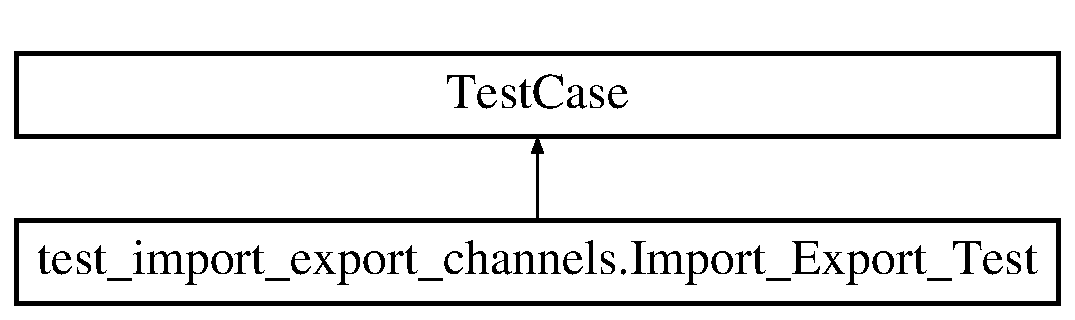
\includegraphics[height=2.000000cm]{classtest__import__export__channels_1_1Import__Export__Test}
\end{center}
\end{figure}
\subsection*{Public Member Functions}
\begin{DoxyCompactItemize}
\item 
def \hyperlink{classtest__import__export__channels_1_1Import__Export__Test_ac8010f3afe7527c5b41c80e8ded8e111}{tear\+Down} (self)
\item 
def \hyperlink{classtest__import__export__channels_1_1Import__Export__Test_a35960ee057b5e68d9b5dd790c44844e4}{test\+\_\+01\+\_\+delete\+\_\+channels\+\_\+data} (self)
\item 
def \hyperlink{classtest__import__export__channels_1_1Import__Export__Test_a773d4cd342672b893c6034109ac1aef1}{test\+\_\+02\+\_\+export\+\_\+channels} (self)
\item 
def \hyperlink{classtest__import__export__channels_1_1Import__Export__Test_a2fe64af468bc4b6e58e8cf0c9faa3bfd}{test\+\_\+03\+\_\+import\+\_\+channels} (self)
\end{DoxyCompactItemize}
\subsection*{Static Public Attributes}
\begin{DoxyCompactItemize}
\item 
\hyperlink{classtest__import__export__channels_1_1Import__Export__Test_a525fbee2a5d043600226e8384f78fde9}{exported\+\_\+data} = None
\item 
\hyperlink{classtest__import__export__channels_1_1Import__Export__Test_a78e070574094839452508d9b8f5589f3}{imported\+\_\+data} = None
\end{DoxyCompactItemize}


\subsection{Member Function Documentation}
\hypertarget{classtest__import__export__channels_1_1Import__Export__Test_ac8010f3afe7527c5b41c80e8ded8e111}{}\index{test\+\_\+import\+\_\+export\+\_\+channels\+::\+Import\+\_\+\+Export\+\_\+\+Test@{test\+\_\+import\+\_\+export\+\_\+channels\+::\+Import\+\_\+\+Export\+\_\+\+Test}!tear\+Down@{tear\+Down}}
\index{tear\+Down@{tear\+Down}!test\+\_\+import\+\_\+export\+\_\+channels\+::\+Import\+\_\+\+Export\+\_\+\+Test@{test\+\_\+import\+\_\+export\+\_\+channels\+::\+Import\+\_\+\+Export\+\_\+\+Test}}
\subsubsection[{tear\+Down}]{\setlength{\rightskip}{0pt plus 5cm}def test\+\_\+import\+\_\+export\+\_\+channels.\+Import\+\_\+\+Export\+\_\+\+Test.\+tear\+Down (
\begin{DoxyParamCaption}
\item[{}]{self}
\end{DoxyParamCaption}
)}\label{classtest__import__export__channels_1_1Import__Export__Test_ac8010f3afe7527c5b41c80e8ded8e111}
\hypertarget{classtest__import__export__channels_1_1Import__Export__Test_a35960ee057b5e68d9b5dd790c44844e4}{}\index{test\+\_\+import\+\_\+export\+\_\+channels\+::\+Import\+\_\+\+Export\+\_\+\+Test@{test\+\_\+import\+\_\+export\+\_\+channels\+::\+Import\+\_\+\+Export\+\_\+\+Test}!test\+\_\+01\+\_\+delete\+\_\+channels\+\_\+data@{test\+\_\+01\+\_\+delete\+\_\+channels\+\_\+data}}
\index{test\+\_\+01\+\_\+delete\+\_\+channels\+\_\+data@{test\+\_\+01\+\_\+delete\+\_\+channels\+\_\+data}!test\+\_\+import\+\_\+export\+\_\+channels\+::\+Import\+\_\+\+Export\+\_\+\+Test@{test\+\_\+import\+\_\+export\+\_\+channels\+::\+Import\+\_\+\+Export\+\_\+\+Test}}
\subsubsection[{test\+\_\+01\+\_\+delete\+\_\+channels\+\_\+data}]{\setlength{\rightskip}{0pt plus 5cm}def test\+\_\+import\+\_\+export\+\_\+channels.\+Import\+\_\+\+Export\+\_\+\+Test.\+test\+\_\+01\+\_\+delete\+\_\+channels\+\_\+data (
\begin{DoxyParamCaption}
\item[{}]{self}
\end{DoxyParamCaption}
)}\label{classtest__import__export__channels_1_1Import__Export__Test_a35960ee057b5e68d9b5dd790c44844e4}
\hypertarget{classtest__import__export__channels_1_1Import__Export__Test_a773d4cd342672b893c6034109ac1aef1}{}\index{test\+\_\+import\+\_\+export\+\_\+channels\+::\+Import\+\_\+\+Export\+\_\+\+Test@{test\+\_\+import\+\_\+export\+\_\+channels\+::\+Import\+\_\+\+Export\+\_\+\+Test}!test\+\_\+02\+\_\+export\+\_\+channels@{test\+\_\+02\+\_\+export\+\_\+channels}}
\index{test\+\_\+02\+\_\+export\+\_\+channels@{test\+\_\+02\+\_\+export\+\_\+channels}!test\+\_\+import\+\_\+export\+\_\+channels\+::\+Import\+\_\+\+Export\+\_\+\+Test@{test\+\_\+import\+\_\+export\+\_\+channels\+::\+Import\+\_\+\+Export\+\_\+\+Test}}
\subsubsection[{test\+\_\+02\+\_\+export\+\_\+channels}]{\setlength{\rightskip}{0pt plus 5cm}def test\+\_\+import\+\_\+export\+\_\+channels.\+Import\+\_\+\+Export\+\_\+\+Test.\+test\+\_\+02\+\_\+export\+\_\+channels (
\begin{DoxyParamCaption}
\item[{}]{self}
\end{DoxyParamCaption}
)}\label{classtest__import__export__channels_1_1Import__Export__Test_a773d4cd342672b893c6034109ac1aef1}
\hypertarget{classtest__import__export__channels_1_1Import__Export__Test_a2fe64af468bc4b6e58e8cf0c9faa3bfd}{}\index{test\+\_\+import\+\_\+export\+\_\+channels\+::\+Import\+\_\+\+Export\+\_\+\+Test@{test\+\_\+import\+\_\+export\+\_\+channels\+::\+Import\+\_\+\+Export\+\_\+\+Test}!test\+\_\+03\+\_\+import\+\_\+channels@{test\+\_\+03\+\_\+import\+\_\+channels}}
\index{test\+\_\+03\+\_\+import\+\_\+channels@{test\+\_\+03\+\_\+import\+\_\+channels}!test\+\_\+import\+\_\+export\+\_\+channels\+::\+Import\+\_\+\+Export\+\_\+\+Test@{test\+\_\+import\+\_\+export\+\_\+channels\+::\+Import\+\_\+\+Export\+\_\+\+Test}}
\subsubsection[{test\+\_\+03\+\_\+import\+\_\+channels}]{\setlength{\rightskip}{0pt plus 5cm}def test\+\_\+import\+\_\+export\+\_\+channels.\+Import\+\_\+\+Export\+\_\+\+Test.\+test\+\_\+03\+\_\+import\+\_\+channels (
\begin{DoxyParamCaption}
\item[{}]{self}
\end{DoxyParamCaption}
)}\label{classtest__import__export__channels_1_1Import__Export__Test_a2fe64af468bc4b6e58e8cf0c9faa3bfd}


\subsection{Member Data Documentation}
\hypertarget{classtest__import__export__channels_1_1Import__Export__Test_a525fbee2a5d043600226e8384f78fde9}{}\index{test\+\_\+import\+\_\+export\+\_\+channels\+::\+Import\+\_\+\+Export\+\_\+\+Test@{test\+\_\+import\+\_\+export\+\_\+channels\+::\+Import\+\_\+\+Export\+\_\+\+Test}!exported\+\_\+data@{exported\+\_\+data}}
\index{exported\+\_\+data@{exported\+\_\+data}!test\+\_\+import\+\_\+export\+\_\+channels\+::\+Import\+\_\+\+Export\+\_\+\+Test@{test\+\_\+import\+\_\+export\+\_\+channels\+::\+Import\+\_\+\+Export\+\_\+\+Test}}
\subsubsection[{exported\+\_\+data}]{\setlength{\rightskip}{0pt plus 5cm}test\+\_\+import\+\_\+export\+\_\+channels.\+Import\+\_\+\+Export\+\_\+\+Test.\+exported\+\_\+data = None\hspace{0.3cm}{\ttfamily [static]}}\label{classtest__import__export__channels_1_1Import__Export__Test_a525fbee2a5d043600226e8384f78fde9}
\hypertarget{classtest__import__export__channels_1_1Import__Export__Test_a78e070574094839452508d9b8f5589f3}{}\index{test\+\_\+import\+\_\+export\+\_\+channels\+::\+Import\+\_\+\+Export\+\_\+\+Test@{test\+\_\+import\+\_\+export\+\_\+channels\+::\+Import\+\_\+\+Export\+\_\+\+Test}!imported\+\_\+data@{imported\+\_\+data}}
\index{imported\+\_\+data@{imported\+\_\+data}!test\+\_\+import\+\_\+export\+\_\+channels\+::\+Import\+\_\+\+Export\+\_\+\+Test@{test\+\_\+import\+\_\+export\+\_\+channels\+::\+Import\+\_\+\+Export\+\_\+\+Test}}
\subsubsection[{imported\+\_\+data}]{\setlength{\rightskip}{0pt plus 5cm}test\+\_\+import\+\_\+export\+\_\+channels.\+Import\+\_\+\+Export\+\_\+\+Test.\+imported\+\_\+data = None\hspace{0.3cm}{\ttfamily [static]}}\label{classtest__import__export__channels_1_1Import__Export__Test_a78e070574094839452508d9b8f5589f3}


The documentation for this class was generated from the following file\+:\begin{DoxyCompactItemize}
\item 
test/channels/\hyperlink{test__import__export__channels_8py}{test\+\_\+import\+\_\+export\+\_\+channels.\+py}\end{DoxyCompactItemize}

\hypertarget{classsrc_1_1lib_1_1vlc_1_1Instance}{}\section{src.\+lib.\+vlc.\+Instance Class Reference}
\label{classsrc_1_1lib_1_1vlc_1_1Instance}\index{src.\+lib.\+vlc.\+Instance@{src.\+lib.\+vlc.\+Instance}}
Inheritance diagram for src.\+lib.\+vlc.\+Instance\+:\begin{figure}[H]
\begin{center}
\leavevmode
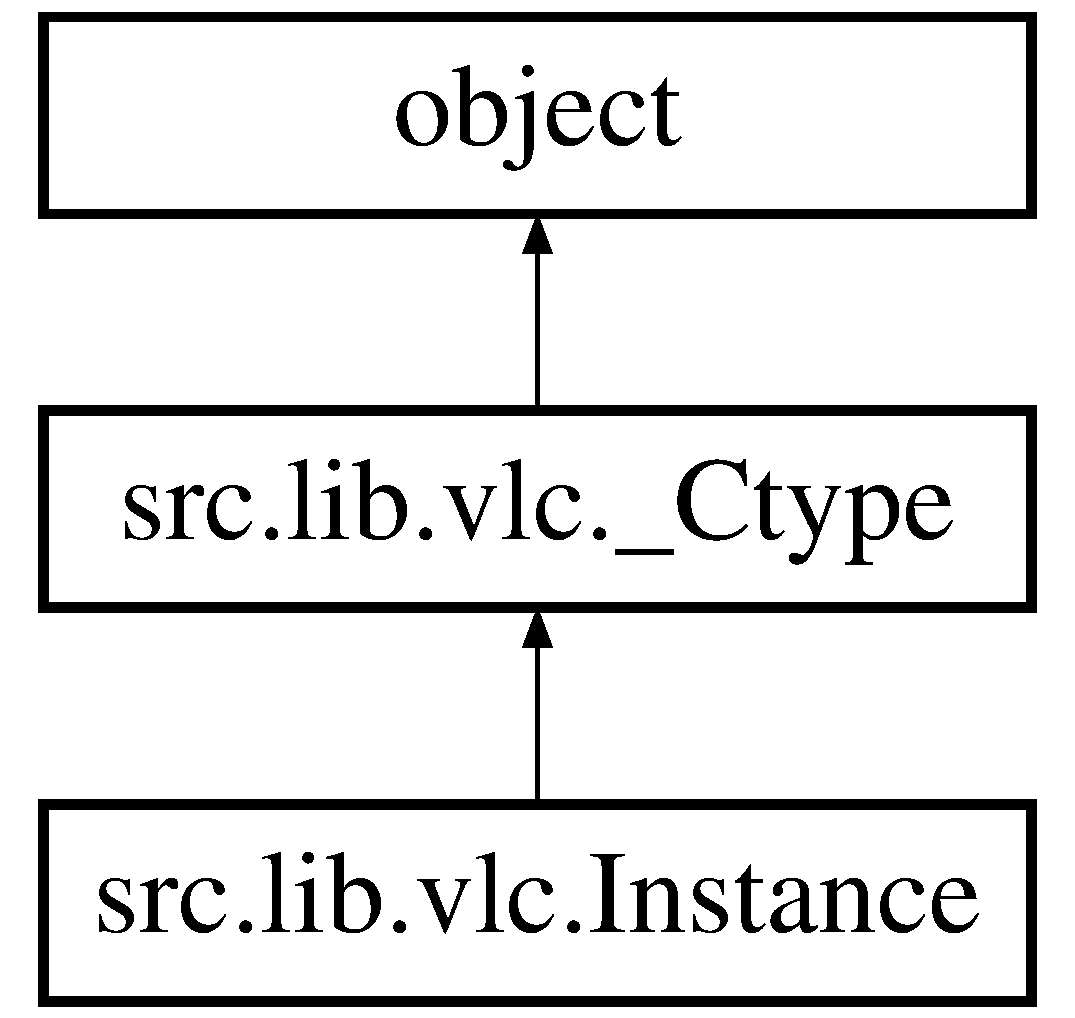
\includegraphics[height=3.000000cm]{classsrc_1_1lib_1_1vlc_1_1Instance}
\end{center}
\end{figure}
\subsection*{Public Member Functions}
\begin{DoxyCompactItemize}
\item 
def \hyperlink{classsrc_1_1lib_1_1vlc_1_1Instance_a6049b5b5c8f5fad4997792e385f1c28b}{\+\_\+\+\_\+new\+\_\+\+\_\+} (cls, args)
\item 
def \hyperlink{classsrc_1_1lib_1_1vlc_1_1Instance_acb31890e7aaf36575e5ec23e7f6ca562}{media\+\_\+player\+\_\+new}
\item 
def \hyperlink{classsrc_1_1lib_1_1vlc_1_1Instance_a7433bcf39b10294cea277502fc72a019}{media\+\_\+list\+\_\+player\+\_\+new} (self)
\item 
def \hyperlink{classsrc_1_1lib_1_1vlc_1_1Instance_a1826a97d104c70587f6f4d7fab96bc81}{media\+\_\+new} (self, mrl, options)
\item 
def \hyperlink{classsrc_1_1lib_1_1vlc_1_1Instance_a44f4fed61bc7bd5920d22f8d7e76ab77}{media\+\_\+list\+\_\+new}
\item 
def \hyperlink{classsrc_1_1lib_1_1vlc_1_1Instance_a91a264abf7ab8cad552a220d38f196fb}{audio\+\_\+output\+\_\+enumerate\+\_\+devices} (self)
\item 
def \hyperlink{classsrc_1_1lib_1_1vlc_1_1Instance_a31b2561af371b849d9711cf5309a205e}{audio\+\_\+filter\+\_\+list\+\_\+get} (self)
\item 
def \hyperlink{classsrc_1_1lib_1_1vlc_1_1Instance_a64321333499e43756da7700a21d58222}{video\+\_\+filter\+\_\+list\+\_\+get} (self)
\item 
def \hyperlink{classsrc_1_1lib_1_1vlc_1_1Instance_a33a79d739d9f61b91291cc6c6c57f20e}{release} (self)
\item 
def \hyperlink{classsrc_1_1lib_1_1vlc_1_1Instance_ab25ffc3a1331b995a8a7429a7a723746}{retain} (self)
\item 
def \hyperlink{classsrc_1_1lib_1_1vlc_1_1Instance_a62258039d44d774f30a922b57a554bf6}{add\+\_\+intf} (self, name)
\item 
def \hyperlink{classsrc_1_1lib_1_1vlc_1_1Instance_ad5ebe431463762bf765d57068920d05b}{wait} (self)
\item 
def \hyperlink{classsrc_1_1lib_1_1vlc_1_1Instance_a3c3df71ad6ccfa88cbb049866ad48797}{set\+\_\+user\+\_\+agent} (self, name, http)
\item 
def \hyperlink{classsrc_1_1lib_1_1vlc_1_1Instance_a94eb5e7343a37a53a95a92f65805445d}{get\+\_\+log\+\_\+verbosity} (self)
\item 
def \hyperlink{classsrc_1_1lib_1_1vlc_1_1Instance_a7336876914fc6252b64032b38baa519b}{set\+\_\+log\+\_\+verbosity} (self, level)
\item 
def \hyperlink{classsrc_1_1lib_1_1vlc_1_1Instance_aac3f845fafe028a1ea5674bea8e35062}{log\+\_\+open} (self)
\item 
def \hyperlink{classsrc_1_1lib_1_1vlc_1_1Instance_a5d53d055dee435d03fccd87cc7ceac54}{media\+\_\+new\+\_\+location} (self, psz\+\_\+mrl)
\item 
def \hyperlink{classsrc_1_1lib_1_1vlc_1_1Instance_ae99efbc23fa602f5f9e942b39167cd7d}{media\+\_\+new\+\_\+path} (self, path)
\item 
def \hyperlink{classsrc_1_1lib_1_1vlc_1_1Instance_a95ba5c11f75a81ce55a87ab2ecc8540d}{media\+\_\+new\+\_\+fd} (self, fd)
\item 
def \hyperlink{classsrc_1_1lib_1_1vlc_1_1Instance_acbd9f11bee08499349ccf2817d6431fb}{media\+\_\+new\+\_\+as\+\_\+node} (self, psz\+\_\+name)
\item 
def \hyperlink{classsrc_1_1lib_1_1vlc_1_1Instance_ab7909c382439a6feab4c8c1017cbc251}{media\+\_\+discoverer\+\_\+new\+\_\+from\+\_\+name} (self, psz\+\_\+name)
\item 
def \hyperlink{classsrc_1_1lib_1_1vlc_1_1Instance_a7ef0d8802a23a731f9c26b590630c6cf}{media\+\_\+library\+\_\+new} (self)
\item 
def \hyperlink{classsrc_1_1lib_1_1vlc_1_1Instance_ae5fb9caf5809300f76a354d9bc8944ad}{audio\+\_\+output\+\_\+list\+\_\+get} (self)
\item 
def \hyperlink{classsrc_1_1lib_1_1vlc_1_1Instance_a714f484b53c481fee361d0ceb5bc8696}{audio\+\_\+output\+\_\+device\+\_\+count} (self, psz\+\_\+audio\+\_\+output)
\item 
def \hyperlink{classsrc_1_1lib_1_1vlc_1_1Instance_a4299934b3829897de26c114459498dc7}{audio\+\_\+output\+\_\+device\+\_\+longname} (self, psz\+\_\+audio\+\_\+output, i\+\_\+device)
\item 
def \hyperlink{classsrc_1_1lib_1_1vlc_1_1Instance_a635b7449ca9172b69051c41c17c6a785}{audio\+\_\+output\+\_\+device\+\_\+id} (self, psz\+\_\+audio\+\_\+output, i\+\_\+device)
\item 
def \hyperlink{classsrc_1_1lib_1_1vlc_1_1Instance_aed1e30f9deffb29435c61bf4503b0ad6}{vlm\+\_\+release} (self)
\item 
def \hyperlink{classsrc_1_1lib_1_1vlc_1_1Instance_a2683025483a5746b5716f02d93f000f3}{vlm\+\_\+add\+\_\+broadcast} (self, psz\+\_\+name, psz\+\_\+input, psz\+\_\+output, i\+\_\+options, ppsz\+\_\+options, b\+\_\+enabled, b\+\_\+loop)
\item 
def \hyperlink{classsrc_1_1lib_1_1vlc_1_1Instance_ad907d65cd7a79ce7a5d955d977cbc25f}{vlm\+\_\+add\+\_\+vod} (self, psz\+\_\+name, psz\+\_\+input, i\+\_\+options, ppsz\+\_\+options, b\+\_\+enabled, psz\+\_\+mux)
\item 
def \hyperlink{classsrc_1_1lib_1_1vlc_1_1Instance_ab8e66804afb92a9c6f3775f4612abb7f}{vlm\+\_\+del\+\_\+media} (self, psz\+\_\+name)
\item 
def \hyperlink{classsrc_1_1lib_1_1vlc_1_1Instance_a599996a68e080c26015912b8fce3633d}{vlm\+\_\+set\+\_\+enabled} (self, psz\+\_\+name, b\+\_\+enabled)
\item 
def \hyperlink{classsrc_1_1lib_1_1vlc_1_1Instance_a8c9c693d3207e845c65bad13c7a27751}{vlm\+\_\+set\+\_\+output} (self, psz\+\_\+name, psz\+\_\+output)
\item 
def \hyperlink{classsrc_1_1lib_1_1vlc_1_1Instance_a76cbc74f54e39271f1c1b4ad9de84449}{vlm\+\_\+set\+\_\+input} (self, psz\+\_\+name, psz\+\_\+input)
\item 
def \hyperlink{classsrc_1_1lib_1_1vlc_1_1Instance_a3fedc984ee9e327665ad0dbba8e2415f}{vlm\+\_\+add\+\_\+input} (self, psz\+\_\+name, psz\+\_\+input)
\item 
def \hyperlink{classsrc_1_1lib_1_1vlc_1_1Instance_a8e01b1f7711324d4702c17c84d7e8523}{vlm\+\_\+set\+\_\+loop} (self, psz\+\_\+name, b\+\_\+loop)
\item 
def \hyperlink{classsrc_1_1lib_1_1vlc_1_1Instance_ab9ba7289b99868457afa42c242ad2448}{vlm\+\_\+set\+\_\+mux} (self, psz\+\_\+name, psz\+\_\+mux)
\item 
def \hyperlink{classsrc_1_1lib_1_1vlc_1_1Instance_a2f8d66071d0fff9fbdb3c38ded9757e2}{vlm\+\_\+change\+\_\+media} (self, psz\+\_\+name, psz\+\_\+input, psz\+\_\+output, i\+\_\+options, ppsz\+\_\+options, b\+\_\+enabled, b\+\_\+loop)
\item 
def \hyperlink{classsrc_1_1lib_1_1vlc_1_1Instance_af1b49067ae43eca760e87d628d41a6a6}{vlm\+\_\+play\+\_\+media} (self, psz\+\_\+name)
\item 
def \hyperlink{classsrc_1_1lib_1_1vlc_1_1Instance_a2ab4493706ea9e3dca240a7512007c93}{vlm\+\_\+stop\+\_\+media} (self, psz\+\_\+name)
\item 
def \hyperlink{classsrc_1_1lib_1_1vlc_1_1Instance_acbfe87cd1265929f796d85edb5df1349}{vlm\+\_\+pause\+\_\+media} (self, psz\+\_\+name)
\item 
def \hyperlink{classsrc_1_1lib_1_1vlc_1_1Instance_ab6930768527cbc0152887132d6b07b48}{vlm\+\_\+seek\+\_\+media} (self, psz\+\_\+name, f\+\_\+percentage)
\item 
def \hyperlink{classsrc_1_1lib_1_1vlc_1_1Instance_a186eb4c98eb5bb12664edf68690987d7}{vlm\+\_\+show\+\_\+media} (self, psz\+\_\+name)
\item 
def \hyperlink{classsrc_1_1lib_1_1vlc_1_1Instance_a6c2f36af97fc8d17f140e69b184ba548}{vlm\+\_\+get\+\_\+media\+\_\+instance\+\_\+position} (self, psz\+\_\+name, i\+\_\+instance)
\item 
def \hyperlink{classsrc_1_1lib_1_1vlc_1_1Instance_af4bd843db6456247187babecc0848810}{vlm\+\_\+get\+\_\+media\+\_\+instance\+\_\+time} (self, psz\+\_\+name, i\+\_\+instance)
\item 
def \hyperlink{classsrc_1_1lib_1_1vlc_1_1Instance_aa9f7c16140978618b2ee70400fa56810}{vlm\+\_\+get\+\_\+media\+\_\+instance\+\_\+length} (self, psz\+\_\+name, i\+\_\+instance)
\item 
def \hyperlink{classsrc_1_1lib_1_1vlc_1_1Instance_a3d8939ebb1774800b8d2045d50d74398}{vlm\+\_\+get\+\_\+media\+\_\+instance\+\_\+rate} (self, psz\+\_\+name, i\+\_\+instance)
\item 
def \hyperlink{classsrc_1_1lib_1_1vlc_1_1Instance_aca3ee8315660645897420e1985f2b737}{vlm\+\_\+get\+\_\+media\+\_\+instance\+\_\+title} (self, psz\+\_\+name, i\+\_\+instance)
\item 
def \hyperlink{classsrc_1_1lib_1_1vlc_1_1Instance_a7743ef391a88ddc83d5de1355fc546d8}{vlm\+\_\+get\+\_\+media\+\_\+instance\+\_\+chapter} (self, psz\+\_\+name, i\+\_\+instance)
\item 
def \hyperlink{classsrc_1_1lib_1_1vlc_1_1Instance_a2e417baee82a23c007f43a0055fa52cb}{vlm\+\_\+get\+\_\+media\+\_\+instance\+\_\+seekable} (self, psz\+\_\+name, i\+\_\+instance)
\item 
def \hyperlink{classsrc_1_1lib_1_1vlc_1_1Instance_aa1330dd3b1aa3da8b40977d36c399c4f}{vlm\+\_\+get\+\_\+event\+\_\+manager} (self)
\end{DoxyCompactItemize}
\subsection*{Additional Inherited Members}


\subsection{Detailed Description}
\begin{DoxyVerb}Create a new Instance instance.

It may take as parameter either:
  - a string
  - a list of strings as first parameters
  - the parameters given as the constructor parameters (must be strings)\end{DoxyVerb}
 

\subsection{Member Function Documentation}
\hypertarget{classsrc_1_1lib_1_1vlc_1_1Instance_a6049b5b5c8f5fad4997792e385f1c28b}{}\index{src\+::lib\+::vlc\+::\+Instance@{src\+::lib\+::vlc\+::\+Instance}!\+\_\+\+\_\+new\+\_\+\+\_\+@{\+\_\+\+\_\+new\+\_\+\+\_\+}}
\index{\+\_\+\+\_\+new\+\_\+\+\_\+@{\+\_\+\+\_\+new\+\_\+\+\_\+}!src\+::lib\+::vlc\+::\+Instance@{src\+::lib\+::vlc\+::\+Instance}}
\subsubsection[{\+\_\+\+\_\+new\+\_\+\+\_\+}]{\setlength{\rightskip}{0pt plus 5cm}def src.\+lib.\+vlc.\+Instance.\+\_\+\+\_\+new\+\_\+\+\_\+ (
\begin{DoxyParamCaption}
\item[{}]{cls, }
\item[{}]{args}
\end{DoxyParamCaption}
)}\label{classsrc_1_1lib_1_1vlc_1_1Instance_a6049b5b5c8f5fad4997792e385f1c28b}
\hypertarget{classsrc_1_1lib_1_1vlc_1_1Instance_a62258039d44d774f30a922b57a554bf6}{}\index{src\+::lib\+::vlc\+::\+Instance@{src\+::lib\+::vlc\+::\+Instance}!add\+\_\+intf@{add\+\_\+intf}}
\index{add\+\_\+intf@{add\+\_\+intf}!src\+::lib\+::vlc\+::\+Instance@{src\+::lib\+::vlc\+::\+Instance}}
\subsubsection[{add\+\_\+intf}]{\setlength{\rightskip}{0pt plus 5cm}def src.\+lib.\+vlc.\+Instance.\+add\+\_\+intf (
\begin{DoxyParamCaption}
\item[{}]{self, }
\item[{}]{name}
\end{DoxyParamCaption}
)}\label{classsrc_1_1lib_1_1vlc_1_1Instance_a62258039d44d774f30a922b57a554bf6}
\begin{DoxyVerb}Try to start a user interface for the libvlc instance.
@param name: interface name, or NULL for default.
@return: 0 on success, -1 on error.
\end{DoxyVerb}
 \hypertarget{classsrc_1_1lib_1_1vlc_1_1Instance_a31b2561af371b849d9711cf5309a205e}{}\index{src\+::lib\+::vlc\+::\+Instance@{src\+::lib\+::vlc\+::\+Instance}!audio\+\_\+filter\+\_\+list\+\_\+get@{audio\+\_\+filter\+\_\+list\+\_\+get}}
\index{audio\+\_\+filter\+\_\+list\+\_\+get@{audio\+\_\+filter\+\_\+list\+\_\+get}!src\+::lib\+::vlc\+::\+Instance@{src\+::lib\+::vlc\+::\+Instance}}
\subsubsection[{audio\+\_\+filter\+\_\+list\+\_\+get}]{\setlength{\rightskip}{0pt plus 5cm}def src.\+lib.\+vlc.\+Instance.\+audio\+\_\+filter\+\_\+list\+\_\+get (
\begin{DoxyParamCaption}
\item[{}]{self}
\end{DoxyParamCaption}
)}\label{classsrc_1_1lib_1_1vlc_1_1Instance_a31b2561af371b849d9711cf5309a205e}
\begin{DoxyVerb}Returns a list of available audio filters.\end{DoxyVerb}
 \hypertarget{classsrc_1_1lib_1_1vlc_1_1Instance_a714f484b53c481fee361d0ceb5bc8696}{}\index{src\+::lib\+::vlc\+::\+Instance@{src\+::lib\+::vlc\+::\+Instance}!audio\+\_\+output\+\_\+device\+\_\+count@{audio\+\_\+output\+\_\+device\+\_\+count}}
\index{audio\+\_\+output\+\_\+device\+\_\+count@{audio\+\_\+output\+\_\+device\+\_\+count}!src\+::lib\+::vlc\+::\+Instance@{src\+::lib\+::vlc\+::\+Instance}}
\subsubsection[{audio\+\_\+output\+\_\+device\+\_\+count}]{\setlength{\rightskip}{0pt plus 5cm}def src.\+lib.\+vlc.\+Instance.\+audio\+\_\+output\+\_\+device\+\_\+count (
\begin{DoxyParamCaption}
\item[{}]{self, }
\item[{}]{psz\+\_\+audio\+\_\+output}
\end{DoxyParamCaption}
)}\label{classsrc_1_1lib_1_1vlc_1_1Instance_a714f484b53c481fee361d0ceb5bc8696}
\begin{DoxyVerb}Get count of devices for audio output, these devices are hardware oriented
like analor or digital output of sound card.
@param psz_audio_output: - name of audio output, See L{AudioOutput}.
@return: number of devices.
\end{DoxyVerb}
 \hypertarget{classsrc_1_1lib_1_1vlc_1_1Instance_a635b7449ca9172b69051c41c17c6a785}{}\index{src\+::lib\+::vlc\+::\+Instance@{src\+::lib\+::vlc\+::\+Instance}!audio\+\_\+output\+\_\+device\+\_\+id@{audio\+\_\+output\+\_\+device\+\_\+id}}
\index{audio\+\_\+output\+\_\+device\+\_\+id@{audio\+\_\+output\+\_\+device\+\_\+id}!src\+::lib\+::vlc\+::\+Instance@{src\+::lib\+::vlc\+::\+Instance}}
\subsubsection[{audio\+\_\+output\+\_\+device\+\_\+id}]{\setlength{\rightskip}{0pt plus 5cm}def src.\+lib.\+vlc.\+Instance.\+audio\+\_\+output\+\_\+device\+\_\+id (
\begin{DoxyParamCaption}
\item[{}]{self, }
\item[{}]{psz\+\_\+audio\+\_\+output, }
\item[{}]{i\+\_\+device}
\end{DoxyParamCaption}
)}\label{classsrc_1_1lib_1_1vlc_1_1Instance_a635b7449ca9172b69051c41c17c6a785}
\begin{DoxyVerb}Get id name of device.
@param psz_audio_output: - name of audio output, See L{AudioOutput}.
@param i_device: device index.
@return: id name of device, use for setting device, need to be free after use.
\end{DoxyVerb}
 \hypertarget{classsrc_1_1lib_1_1vlc_1_1Instance_a4299934b3829897de26c114459498dc7}{}\index{src\+::lib\+::vlc\+::\+Instance@{src\+::lib\+::vlc\+::\+Instance}!audio\+\_\+output\+\_\+device\+\_\+longname@{audio\+\_\+output\+\_\+device\+\_\+longname}}
\index{audio\+\_\+output\+\_\+device\+\_\+longname@{audio\+\_\+output\+\_\+device\+\_\+longname}!src\+::lib\+::vlc\+::\+Instance@{src\+::lib\+::vlc\+::\+Instance}}
\subsubsection[{audio\+\_\+output\+\_\+device\+\_\+longname}]{\setlength{\rightskip}{0pt plus 5cm}def src.\+lib.\+vlc.\+Instance.\+audio\+\_\+output\+\_\+device\+\_\+longname (
\begin{DoxyParamCaption}
\item[{}]{self, }
\item[{}]{psz\+\_\+audio\+\_\+output, }
\item[{}]{i\+\_\+device}
\end{DoxyParamCaption}
)}\label{classsrc_1_1lib_1_1vlc_1_1Instance_a4299934b3829897de26c114459498dc7}
\begin{DoxyVerb}Get long name of device, if not available short name given.
@param psz_audio_output: - name of audio output, See L{AudioOutput}.
@param i_device: device index.
@return: long name of device.
\end{DoxyVerb}
 \hypertarget{classsrc_1_1lib_1_1vlc_1_1Instance_a91a264abf7ab8cad552a220d38f196fb}{}\index{src\+::lib\+::vlc\+::\+Instance@{src\+::lib\+::vlc\+::\+Instance}!audio\+\_\+output\+\_\+enumerate\+\_\+devices@{audio\+\_\+output\+\_\+enumerate\+\_\+devices}}
\index{audio\+\_\+output\+\_\+enumerate\+\_\+devices@{audio\+\_\+output\+\_\+enumerate\+\_\+devices}!src\+::lib\+::vlc\+::\+Instance@{src\+::lib\+::vlc\+::\+Instance}}
\subsubsection[{audio\+\_\+output\+\_\+enumerate\+\_\+devices}]{\setlength{\rightskip}{0pt plus 5cm}def src.\+lib.\+vlc.\+Instance.\+audio\+\_\+output\+\_\+enumerate\+\_\+devices (
\begin{DoxyParamCaption}
\item[{}]{self}
\end{DoxyParamCaption}
)}\label{classsrc_1_1lib_1_1vlc_1_1Instance_a91a264abf7ab8cad552a220d38f196fb}
\begin{DoxyVerb}Enumerate the defined audio output devices.

@return: list of dicts {name:, description:, devices:}
\end{DoxyVerb}
 \hypertarget{classsrc_1_1lib_1_1vlc_1_1Instance_ae5fb9caf5809300f76a354d9bc8944ad}{}\index{src\+::lib\+::vlc\+::\+Instance@{src\+::lib\+::vlc\+::\+Instance}!audio\+\_\+output\+\_\+list\+\_\+get@{audio\+\_\+output\+\_\+list\+\_\+get}}
\index{audio\+\_\+output\+\_\+list\+\_\+get@{audio\+\_\+output\+\_\+list\+\_\+get}!src\+::lib\+::vlc\+::\+Instance@{src\+::lib\+::vlc\+::\+Instance}}
\subsubsection[{audio\+\_\+output\+\_\+list\+\_\+get}]{\setlength{\rightskip}{0pt plus 5cm}def src.\+lib.\+vlc.\+Instance.\+audio\+\_\+output\+\_\+list\+\_\+get (
\begin{DoxyParamCaption}
\item[{}]{self}
\end{DoxyParamCaption}
)}\label{classsrc_1_1lib_1_1vlc_1_1Instance_ae5fb9caf5809300f76a354d9bc8944ad}
\begin{DoxyVerb}Get the list of available audio outputs.
@return: list of available audio outputs. It must be freed it with In case of error, NULL is returned.
\end{DoxyVerb}
 \hypertarget{classsrc_1_1lib_1_1vlc_1_1Instance_a94eb5e7343a37a53a95a92f65805445d}{}\index{src\+::lib\+::vlc\+::\+Instance@{src\+::lib\+::vlc\+::\+Instance}!get\+\_\+log\+\_\+verbosity@{get\+\_\+log\+\_\+verbosity}}
\index{get\+\_\+log\+\_\+verbosity@{get\+\_\+log\+\_\+verbosity}!src\+::lib\+::vlc\+::\+Instance@{src\+::lib\+::vlc\+::\+Instance}}
\subsubsection[{get\+\_\+log\+\_\+verbosity}]{\setlength{\rightskip}{0pt plus 5cm}def src.\+lib.\+vlc.\+Instance.\+get\+\_\+log\+\_\+verbosity (
\begin{DoxyParamCaption}
\item[{}]{self}
\end{DoxyParamCaption}
)}\label{classsrc_1_1lib_1_1vlc_1_1Instance_a94eb5e7343a37a53a95a92f65805445d}
\begin{DoxyVerb}Always returns minus one.
This function is only provided for backward compatibility.
@return: always -1.
\end{DoxyVerb}
 \hypertarget{classsrc_1_1lib_1_1vlc_1_1Instance_aac3f845fafe028a1ea5674bea8e35062}{}\index{src\+::lib\+::vlc\+::\+Instance@{src\+::lib\+::vlc\+::\+Instance}!log\+\_\+open@{log\+\_\+open}}
\index{log\+\_\+open@{log\+\_\+open}!src\+::lib\+::vlc\+::\+Instance@{src\+::lib\+::vlc\+::\+Instance}}
\subsubsection[{log\+\_\+open}]{\setlength{\rightskip}{0pt plus 5cm}def src.\+lib.\+vlc.\+Instance.\+log\+\_\+open (
\begin{DoxyParamCaption}
\item[{}]{self}
\end{DoxyParamCaption}
)}\label{classsrc_1_1lib_1_1vlc_1_1Instance_aac3f845fafe028a1ea5674bea8e35062}
\begin{DoxyVerb}This function does nothing useful.
It is only provided for backward compatibility.
@return: an unique pointer or NULL on error.
\end{DoxyVerb}
 \hypertarget{classsrc_1_1lib_1_1vlc_1_1Instance_ab7909c382439a6feab4c8c1017cbc251}{}\index{src\+::lib\+::vlc\+::\+Instance@{src\+::lib\+::vlc\+::\+Instance}!media\+\_\+discoverer\+\_\+new\+\_\+from\+\_\+name@{media\+\_\+discoverer\+\_\+new\+\_\+from\+\_\+name}}
\index{media\+\_\+discoverer\+\_\+new\+\_\+from\+\_\+name@{media\+\_\+discoverer\+\_\+new\+\_\+from\+\_\+name}!src\+::lib\+::vlc\+::\+Instance@{src\+::lib\+::vlc\+::\+Instance}}
\subsubsection[{media\+\_\+discoverer\+\_\+new\+\_\+from\+\_\+name}]{\setlength{\rightskip}{0pt plus 5cm}def src.\+lib.\+vlc.\+Instance.\+media\+\_\+discoverer\+\_\+new\+\_\+from\+\_\+name (
\begin{DoxyParamCaption}
\item[{}]{self, }
\item[{}]{psz\+\_\+name}
\end{DoxyParamCaption}
)}\label{classsrc_1_1lib_1_1vlc_1_1Instance_ab7909c382439a6feab4c8c1017cbc251}
\begin{DoxyVerb}Discover media service by name.
@param psz_name: service name.
@return: media discover object or NULL in case of error.
\end{DoxyVerb}
 \hypertarget{classsrc_1_1lib_1_1vlc_1_1Instance_a7ef0d8802a23a731f9c26b590630c6cf}{}\index{src\+::lib\+::vlc\+::\+Instance@{src\+::lib\+::vlc\+::\+Instance}!media\+\_\+library\+\_\+new@{media\+\_\+library\+\_\+new}}
\index{media\+\_\+library\+\_\+new@{media\+\_\+library\+\_\+new}!src\+::lib\+::vlc\+::\+Instance@{src\+::lib\+::vlc\+::\+Instance}}
\subsubsection[{media\+\_\+library\+\_\+new}]{\setlength{\rightskip}{0pt plus 5cm}def src.\+lib.\+vlc.\+Instance.\+media\+\_\+library\+\_\+new (
\begin{DoxyParamCaption}
\item[{}]{self}
\end{DoxyParamCaption}
)}\label{classsrc_1_1lib_1_1vlc_1_1Instance_a7ef0d8802a23a731f9c26b590630c6cf}
\begin{DoxyVerb}Create an new Media Library object.
@return: a new object or NULL on error.
\end{DoxyVerb}
 \hypertarget{classsrc_1_1lib_1_1vlc_1_1Instance_a44f4fed61bc7bd5920d22f8d7e76ab77}{}\index{src\+::lib\+::vlc\+::\+Instance@{src\+::lib\+::vlc\+::\+Instance}!media\+\_\+list\+\_\+new@{media\+\_\+list\+\_\+new}}
\index{media\+\_\+list\+\_\+new@{media\+\_\+list\+\_\+new}!src\+::lib\+::vlc\+::\+Instance@{src\+::lib\+::vlc\+::\+Instance}}
\subsubsection[{media\+\_\+list\+\_\+new}]{\setlength{\rightskip}{0pt plus 5cm}def src.\+lib.\+vlc.\+Instance.\+media\+\_\+list\+\_\+new (
\begin{DoxyParamCaption}
\item[{}]{self, }
\item[{}]{mrls = {\ttfamily None}}
\end{DoxyParamCaption}
)}\label{classsrc_1_1lib_1_1vlc_1_1Instance_a44f4fed61bc7bd5920d22f8d7e76ab77}
\begin{DoxyVerb}Create a new MediaList instance.
@param mrls: optional list of MRL strings
\end{DoxyVerb}
 \hypertarget{classsrc_1_1lib_1_1vlc_1_1Instance_a7433bcf39b10294cea277502fc72a019}{}\index{src\+::lib\+::vlc\+::\+Instance@{src\+::lib\+::vlc\+::\+Instance}!media\+\_\+list\+\_\+player\+\_\+new@{media\+\_\+list\+\_\+player\+\_\+new}}
\index{media\+\_\+list\+\_\+player\+\_\+new@{media\+\_\+list\+\_\+player\+\_\+new}!src\+::lib\+::vlc\+::\+Instance@{src\+::lib\+::vlc\+::\+Instance}}
\subsubsection[{media\+\_\+list\+\_\+player\+\_\+new}]{\setlength{\rightskip}{0pt plus 5cm}def src.\+lib.\+vlc.\+Instance.\+media\+\_\+list\+\_\+player\+\_\+new (
\begin{DoxyParamCaption}
\item[{}]{self}
\end{DoxyParamCaption}
)}\label{classsrc_1_1lib_1_1vlc_1_1Instance_a7433bcf39b10294cea277502fc72a019}
\begin{DoxyVerb}Create a new MediaListPlayer instance.
\end{DoxyVerb}
 \hypertarget{classsrc_1_1lib_1_1vlc_1_1Instance_a1826a97d104c70587f6f4d7fab96bc81}{}\index{src\+::lib\+::vlc\+::\+Instance@{src\+::lib\+::vlc\+::\+Instance}!media\+\_\+new@{media\+\_\+new}}
\index{media\+\_\+new@{media\+\_\+new}!src\+::lib\+::vlc\+::\+Instance@{src\+::lib\+::vlc\+::\+Instance}}
\subsubsection[{media\+\_\+new}]{\setlength{\rightskip}{0pt plus 5cm}def src.\+lib.\+vlc.\+Instance.\+media\+\_\+new (
\begin{DoxyParamCaption}
\item[{}]{self, }
\item[{}]{mrl, }
\item[{}]{options}
\end{DoxyParamCaption}
)}\label{classsrc_1_1lib_1_1vlc_1_1Instance_a1826a97d104c70587f6f4d7fab96bc81}
\begin{DoxyVerb}Create a new Media instance.

If mrl contains a colon (:) preceded by more than 1 letter, it
will be treated as a URL. Else, it will be considered as a
local path. If you need more control, directly use
media_new_location/media_new_path methods.

Options can be specified as supplementary string parameters, e.g.

C{m = i.media_new('foo.avi', 'sub-filter=marq{marquee=Hello}', 'vout-filter=invert')}

Alternatively, the options can be added to the media using the Media.add_options method:

C{m.add_options('foo.avi', 'sub-filter=marq@test{marquee=Hello}', 'video-filter=invert')}

@param options: optional media option=value strings
\end{DoxyVerb}
 \hypertarget{classsrc_1_1lib_1_1vlc_1_1Instance_acbd9f11bee08499349ccf2817d6431fb}{}\index{src\+::lib\+::vlc\+::\+Instance@{src\+::lib\+::vlc\+::\+Instance}!media\+\_\+new\+\_\+as\+\_\+node@{media\+\_\+new\+\_\+as\+\_\+node}}
\index{media\+\_\+new\+\_\+as\+\_\+node@{media\+\_\+new\+\_\+as\+\_\+node}!src\+::lib\+::vlc\+::\+Instance@{src\+::lib\+::vlc\+::\+Instance}}
\subsubsection[{media\+\_\+new\+\_\+as\+\_\+node}]{\setlength{\rightskip}{0pt plus 5cm}def src.\+lib.\+vlc.\+Instance.\+media\+\_\+new\+\_\+as\+\_\+node (
\begin{DoxyParamCaption}
\item[{}]{self, }
\item[{}]{psz\+\_\+name}
\end{DoxyParamCaption}
)}\label{classsrc_1_1lib_1_1vlc_1_1Instance_acbd9f11bee08499349ccf2817d6431fb}
\begin{DoxyVerb}Create a media as an empty node with a given name.
See L{media_release}.
@param psz_name: the name of the node.
@return: the new empty media or NULL on error.
\end{DoxyVerb}
 \hypertarget{classsrc_1_1lib_1_1vlc_1_1Instance_a95ba5c11f75a81ce55a87ab2ecc8540d}{}\index{src\+::lib\+::vlc\+::\+Instance@{src\+::lib\+::vlc\+::\+Instance}!media\+\_\+new\+\_\+fd@{media\+\_\+new\+\_\+fd}}
\index{media\+\_\+new\+\_\+fd@{media\+\_\+new\+\_\+fd}!src\+::lib\+::vlc\+::\+Instance@{src\+::lib\+::vlc\+::\+Instance}}
\subsubsection[{media\+\_\+new\+\_\+fd}]{\setlength{\rightskip}{0pt plus 5cm}def src.\+lib.\+vlc.\+Instance.\+media\+\_\+new\+\_\+fd (
\begin{DoxyParamCaption}
\item[{}]{self, }
\item[{}]{fd}
\end{DoxyParamCaption}
)}\label{classsrc_1_1lib_1_1vlc_1_1Instance_a95ba5c11f75a81ce55a87ab2ecc8540d}
\begin{DoxyVerb}Create a media for an already open file descriptor.
The file descriptor shall be open for reading (or reading and writing).
Regular file descriptors, pipe read descriptors and character device
descriptors (including TTYs) are supported on all platforms.
Block device descriptors are supported where available.
Directory descriptors are supported on systems that provide fdopendir().
Sockets are supported on all platforms where they are file descriptors,
i.e. all except Windows.
@note: This library will B{not} automatically close the file descriptor
under any circumstance. Nevertheless, a file descriptor can usually only be
rendered once in a media player. To render it a second time, the file
descriptor should probably be rewound to the beginning with lseek().
See L{media_release}.
@param fd: open file descriptor.
@return: the newly created media or NULL on error.
@version: LibVLC 1.1.5 and later.
\end{DoxyVerb}
 \hypertarget{classsrc_1_1lib_1_1vlc_1_1Instance_a5d53d055dee435d03fccd87cc7ceac54}{}\index{src\+::lib\+::vlc\+::\+Instance@{src\+::lib\+::vlc\+::\+Instance}!media\+\_\+new\+\_\+location@{media\+\_\+new\+\_\+location}}
\index{media\+\_\+new\+\_\+location@{media\+\_\+new\+\_\+location}!src\+::lib\+::vlc\+::\+Instance@{src\+::lib\+::vlc\+::\+Instance}}
\subsubsection[{media\+\_\+new\+\_\+location}]{\setlength{\rightskip}{0pt plus 5cm}def src.\+lib.\+vlc.\+Instance.\+media\+\_\+new\+\_\+location (
\begin{DoxyParamCaption}
\item[{}]{self, }
\item[{}]{psz\+\_\+mrl}
\end{DoxyParamCaption}
)}\label{classsrc_1_1lib_1_1vlc_1_1Instance_a5d53d055dee435d03fccd87cc7ceac54}
\begin{DoxyVerb}Create a media with a certain given media resource location,
for instance a valid URL.
@note: To refer to a local file with this function,
the file://... URI syntax B{must} be used (see IETF RFC3986).
We recommend using L{media_new_path}() instead when dealing with
local files.
See L{media_release}.
@param psz_mrl: the media location.
@return: the newly created media or NULL on error.
\end{DoxyVerb}
 \hypertarget{classsrc_1_1lib_1_1vlc_1_1Instance_ae99efbc23fa602f5f9e942b39167cd7d}{}\index{src\+::lib\+::vlc\+::\+Instance@{src\+::lib\+::vlc\+::\+Instance}!media\+\_\+new\+\_\+path@{media\+\_\+new\+\_\+path}}
\index{media\+\_\+new\+\_\+path@{media\+\_\+new\+\_\+path}!src\+::lib\+::vlc\+::\+Instance@{src\+::lib\+::vlc\+::\+Instance}}
\subsubsection[{media\+\_\+new\+\_\+path}]{\setlength{\rightskip}{0pt plus 5cm}def src.\+lib.\+vlc.\+Instance.\+media\+\_\+new\+\_\+path (
\begin{DoxyParamCaption}
\item[{}]{self, }
\item[{}]{path}
\end{DoxyParamCaption}
)}\label{classsrc_1_1lib_1_1vlc_1_1Instance_ae99efbc23fa602f5f9e942b39167cd7d}
\begin{DoxyVerb}Create a media for a certain file path.
See L{media_release}.
@param path: local filesystem path.
@return: the newly created media or NULL on error.
\end{DoxyVerb}
 \hypertarget{classsrc_1_1lib_1_1vlc_1_1Instance_acb31890e7aaf36575e5ec23e7f6ca562}{}\index{src\+::lib\+::vlc\+::\+Instance@{src\+::lib\+::vlc\+::\+Instance}!media\+\_\+player\+\_\+new@{media\+\_\+player\+\_\+new}}
\index{media\+\_\+player\+\_\+new@{media\+\_\+player\+\_\+new}!src\+::lib\+::vlc\+::\+Instance@{src\+::lib\+::vlc\+::\+Instance}}
\subsubsection[{media\+\_\+player\+\_\+new}]{\setlength{\rightskip}{0pt plus 5cm}def src.\+lib.\+vlc.\+Instance.\+media\+\_\+player\+\_\+new (
\begin{DoxyParamCaption}
\item[{}]{self, }
\item[{}]{uri = {\ttfamily None}}
\end{DoxyParamCaption}
)}\label{classsrc_1_1lib_1_1vlc_1_1Instance_acb31890e7aaf36575e5ec23e7f6ca562}
\begin{DoxyVerb}Create a new MediaPlayer instance.

@param uri: an optional URI to play in the player.
\end{DoxyVerb}
 \hypertarget{classsrc_1_1lib_1_1vlc_1_1Instance_a33a79d739d9f61b91291cc6c6c57f20e}{}\index{src\+::lib\+::vlc\+::\+Instance@{src\+::lib\+::vlc\+::\+Instance}!release@{release}}
\index{release@{release}!src\+::lib\+::vlc\+::\+Instance@{src\+::lib\+::vlc\+::\+Instance}}
\subsubsection[{release}]{\setlength{\rightskip}{0pt plus 5cm}def src.\+lib.\+vlc.\+Instance.\+release (
\begin{DoxyParamCaption}
\item[{}]{self}
\end{DoxyParamCaption}
)}\label{classsrc_1_1lib_1_1vlc_1_1Instance_a33a79d739d9f61b91291cc6c6c57f20e}
\begin{DoxyVerb}Decrement the reference count of a libvlc instance, and destroy it
if it reaches zero.
\end{DoxyVerb}
 \hypertarget{classsrc_1_1lib_1_1vlc_1_1Instance_ab25ffc3a1331b995a8a7429a7a723746}{}\index{src\+::lib\+::vlc\+::\+Instance@{src\+::lib\+::vlc\+::\+Instance}!retain@{retain}}
\index{retain@{retain}!src\+::lib\+::vlc\+::\+Instance@{src\+::lib\+::vlc\+::\+Instance}}
\subsubsection[{retain}]{\setlength{\rightskip}{0pt plus 5cm}def src.\+lib.\+vlc.\+Instance.\+retain (
\begin{DoxyParamCaption}
\item[{}]{self}
\end{DoxyParamCaption}
)}\label{classsrc_1_1lib_1_1vlc_1_1Instance_ab25ffc3a1331b995a8a7429a7a723746}
\begin{DoxyVerb}Increments the reference count of a libvlc instance.
The initial reference count is 1 after L{new}() returns.
\end{DoxyVerb}
 \hypertarget{classsrc_1_1lib_1_1vlc_1_1Instance_a7336876914fc6252b64032b38baa519b}{}\index{src\+::lib\+::vlc\+::\+Instance@{src\+::lib\+::vlc\+::\+Instance}!set\+\_\+log\+\_\+verbosity@{set\+\_\+log\+\_\+verbosity}}
\index{set\+\_\+log\+\_\+verbosity@{set\+\_\+log\+\_\+verbosity}!src\+::lib\+::vlc\+::\+Instance@{src\+::lib\+::vlc\+::\+Instance}}
\subsubsection[{set\+\_\+log\+\_\+verbosity}]{\setlength{\rightskip}{0pt plus 5cm}def src.\+lib.\+vlc.\+Instance.\+set\+\_\+log\+\_\+verbosity (
\begin{DoxyParamCaption}
\item[{}]{self, }
\item[{}]{level}
\end{DoxyParamCaption}
)}\label{classsrc_1_1lib_1_1vlc_1_1Instance_a7336876914fc6252b64032b38baa519b}
\begin{DoxyVerb}This function does nothing.
It is only provided for backward compatibility.
@param level: ignored.
\end{DoxyVerb}
 \hypertarget{classsrc_1_1lib_1_1vlc_1_1Instance_a3c3df71ad6ccfa88cbb049866ad48797}{}\index{src\+::lib\+::vlc\+::\+Instance@{src\+::lib\+::vlc\+::\+Instance}!set\+\_\+user\+\_\+agent@{set\+\_\+user\+\_\+agent}}
\index{set\+\_\+user\+\_\+agent@{set\+\_\+user\+\_\+agent}!src\+::lib\+::vlc\+::\+Instance@{src\+::lib\+::vlc\+::\+Instance}}
\subsubsection[{set\+\_\+user\+\_\+agent}]{\setlength{\rightskip}{0pt plus 5cm}def src.\+lib.\+vlc.\+Instance.\+set\+\_\+user\+\_\+agent (
\begin{DoxyParamCaption}
\item[{}]{self, }
\item[{}]{name, }
\item[{}]{http}
\end{DoxyParamCaption}
)}\label{classsrc_1_1lib_1_1vlc_1_1Instance_a3c3df71ad6ccfa88cbb049866ad48797}
\begin{DoxyVerb}Sets the application name. LibVLC passes this as the user agent string
when a protocol requires it.
@param name: human-readable application name, e.g. "FooBar player 1.2.3".
@param http: HTTP User Agent, e.g. "FooBar/1.2.3 Python/2.6.0".
@version: LibVLC 1.1.1 or later.
\end{DoxyVerb}
 \hypertarget{classsrc_1_1lib_1_1vlc_1_1Instance_a64321333499e43756da7700a21d58222}{}\index{src\+::lib\+::vlc\+::\+Instance@{src\+::lib\+::vlc\+::\+Instance}!video\+\_\+filter\+\_\+list\+\_\+get@{video\+\_\+filter\+\_\+list\+\_\+get}}
\index{video\+\_\+filter\+\_\+list\+\_\+get@{video\+\_\+filter\+\_\+list\+\_\+get}!src\+::lib\+::vlc\+::\+Instance@{src\+::lib\+::vlc\+::\+Instance}}
\subsubsection[{video\+\_\+filter\+\_\+list\+\_\+get}]{\setlength{\rightskip}{0pt plus 5cm}def src.\+lib.\+vlc.\+Instance.\+video\+\_\+filter\+\_\+list\+\_\+get (
\begin{DoxyParamCaption}
\item[{}]{self}
\end{DoxyParamCaption}
)}\label{classsrc_1_1lib_1_1vlc_1_1Instance_a64321333499e43756da7700a21d58222}
\begin{DoxyVerb}Returns a list of available video filters.\end{DoxyVerb}
 \hypertarget{classsrc_1_1lib_1_1vlc_1_1Instance_a2683025483a5746b5716f02d93f000f3}{}\index{src\+::lib\+::vlc\+::\+Instance@{src\+::lib\+::vlc\+::\+Instance}!vlm\+\_\+add\+\_\+broadcast@{vlm\+\_\+add\+\_\+broadcast}}
\index{vlm\+\_\+add\+\_\+broadcast@{vlm\+\_\+add\+\_\+broadcast}!src\+::lib\+::vlc\+::\+Instance@{src\+::lib\+::vlc\+::\+Instance}}
\subsubsection[{vlm\+\_\+add\+\_\+broadcast}]{\setlength{\rightskip}{0pt plus 5cm}def src.\+lib.\+vlc.\+Instance.\+vlm\+\_\+add\+\_\+broadcast (
\begin{DoxyParamCaption}
\item[{}]{self, }
\item[{}]{psz\+\_\+name, }
\item[{}]{psz\+\_\+input, }
\item[{}]{psz\+\_\+output, }
\item[{}]{i\+\_\+options, }
\item[{}]{ppsz\+\_\+options, }
\item[{}]{b\+\_\+enabled, }
\item[{}]{b\+\_\+loop}
\end{DoxyParamCaption}
)}\label{classsrc_1_1lib_1_1vlc_1_1Instance_a2683025483a5746b5716f02d93f000f3}
\begin{DoxyVerb}Add a broadcast, with one input.
@param psz_name: the name of the new broadcast.
@param psz_input: the input MRL.
@param psz_output: the output MRL (the parameter to the "sout" variable).
@param i_options: number of additional options.
@param ppsz_options: additional options.
@param b_enabled: boolean for enabling the new broadcast.
@param b_loop: Should this broadcast be played in loop ?
@return: 0 on success, -1 on error.
\end{DoxyVerb}
 \hypertarget{classsrc_1_1lib_1_1vlc_1_1Instance_a3fedc984ee9e327665ad0dbba8e2415f}{}\index{src\+::lib\+::vlc\+::\+Instance@{src\+::lib\+::vlc\+::\+Instance}!vlm\+\_\+add\+\_\+input@{vlm\+\_\+add\+\_\+input}}
\index{vlm\+\_\+add\+\_\+input@{vlm\+\_\+add\+\_\+input}!src\+::lib\+::vlc\+::\+Instance@{src\+::lib\+::vlc\+::\+Instance}}
\subsubsection[{vlm\+\_\+add\+\_\+input}]{\setlength{\rightskip}{0pt plus 5cm}def src.\+lib.\+vlc.\+Instance.\+vlm\+\_\+add\+\_\+input (
\begin{DoxyParamCaption}
\item[{}]{self, }
\item[{}]{psz\+\_\+name, }
\item[{}]{psz\+\_\+input}
\end{DoxyParamCaption}
)}\label{classsrc_1_1lib_1_1vlc_1_1Instance_a3fedc984ee9e327665ad0dbba8e2415f}
\begin{DoxyVerb}Add a media's input MRL. This will add the specified one.
@param psz_name: the media to work on.
@param psz_input: the input MRL.
@return: 0 on success, -1 on error.
\end{DoxyVerb}
 \hypertarget{classsrc_1_1lib_1_1vlc_1_1Instance_ad907d65cd7a79ce7a5d955d977cbc25f}{}\index{src\+::lib\+::vlc\+::\+Instance@{src\+::lib\+::vlc\+::\+Instance}!vlm\+\_\+add\+\_\+vod@{vlm\+\_\+add\+\_\+vod}}
\index{vlm\+\_\+add\+\_\+vod@{vlm\+\_\+add\+\_\+vod}!src\+::lib\+::vlc\+::\+Instance@{src\+::lib\+::vlc\+::\+Instance}}
\subsubsection[{vlm\+\_\+add\+\_\+vod}]{\setlength{\rightskip}{0pt plus 5cm}def src.\+lib.\+vlc.\+Instance.\+vlm\+\_\+add\+\_\+vod (
\begin{DoxyParamCaption}
\item[{}]{self, }
\item[{}]{psz\+\_\+name, }
\item[{}]{psz\+\_\+input, }
\item[{}]{i\+\_\+options, }
\item[{}]{ppsz\+\_\+options, }
\item[{}]{b\+\_\+enabled, }
\item[{}]{psz\+\_\+mux}
\end{DoxyParamCaption}
)}\label{classsrc_1_1lib_1_1vlc_1_1Instance_ad907d65cd7a79ce7a5d955d977cbc25f}
\begin{DoxyVerb}Add a vod, with one input.
@param psz_name: the name of the new vod media.
@param psz_input: the input MRL.
@param i_options: number of additional options.
@param ppsz_options: additional options.
@param b_enabled: boolean for enabling the new vod.
@param psz_mux: the muxer of the vod media.
@return: 0 on success, -1 on error.
\end{DoxyVerb}
 \hypertarget{classsrc_1_1lib_1_1vlc_1_1Instance_a2f8d66071d0fff9fbdb3c38ded9757e2}{}\index{src\+::lib\+::vlc\+::\+Instance@{src\+::lib\+::vlc\+::\+Instance}!vlm\+\_\+change\+\_\+media@{vlm\+\_\+change\+\_\+media}}
\index{vlm\+\_\+change\+\_\+media@{vlm\+\_\+change\+\_\+media}!src\+::lib\+::vlc\+::\+Instance@{src\+::lib\+::vlc\+::\+Instance}}
\subsubsection[{vlm\+\_\+change\+\_\+media}]{\setlength{\rightskip}{0pt plus 5cm}def src.\+lib.\+vlc.\+Instance.\+vlm\+\_\+change\+\_\+media (
\begin{DoxyParamCaption}
\item[{}]{self, }
\item[{}]{psz\+\_\+name, }
\item[{}]{psz\+\_\+input, }
\item[{}]{psz\+\_\+output, }
\item[{}]{i\+\_\+options, }
\item[{}]{ppsz\+\_\+options, }
\item[{}]{b\+\_\+enabled, }
\item[{}]{b\+\_\+loop}
\end{DoxyParamCaption}
)}\label{classsrc_1_1lib_1_1vlc_1_1Instance_a2f8d66071d0fff9fbdb3c38ded9757e2}
\begin{DoxyVerb}Edit the parameters of a media. This will delete all existing inputs and
add the specified one.
@param psz_name: the name of the new broadcast.
@param psz_input: the input MRL.
@param psz_output: the output MRL (the parameter to the "sout" variable).
@param i_options: number of additional options.
@param ppsz_options: additional options.
@param b_enabled: boolean for enabling the new broadcast.
@param b_loop: Should this broadcast be played in loop ?
@return: 0 on success, -1 on error.
\end{DoxyVerb}
 \hypertarget{classsrc_1_1lib_1_1vlc_1_1Instance_ab8e66804afb92a9c6f3775f4612abb7f}{}\index{src\+::lib\+::vlc\+::\+Instance@{src\+::lib\+::vlc\+::\+Instance}!vlm\+\_\+del\+\_\+media@{vlm\+\_\+del\+\_\+media}}
\index{vlm\+\_\+del\+\_\+media@{vlm\+\_\+del\+\_\+media}!src\+::lib\+::vlc\+::\+Instance@{src\+::lib\+::vlc\+::\+Instance}}
\subsubsection[{vlm\+\_\+del\+\_\+media}]{\setlength{\rightskip}{0pt plus 5cm}def src.\+lib.\+vlc.\+Instance.\+vlm\+\_\+del\+\_\+media (
\begin{DoxyParamCaption}
\item[{}]{self, }
\item[{}]{psz\+\_\+name}
\end{DoxyParamCaption}
)}\label{classsrc_1_1lib_1_1vlc_1_1Instance_ab8e66804afb92a9c6f3775f4612abb7f}
\begin{DoxyVerb}Delete a media (VOD or broadcast).
@param psz_name: the media to delete.
@return: 0 on success, -1 on error.
\end{DoxyVerb}
 \hypertarget{classsrc_1_1lib_1_1vlc_1_1Instance_aa1330dd3b1aa3da8b40977d36c399c4f}{}\index{src\+::lib\+::vlc\+::\+Instance@{src\+::lib\+::vlc\+::\+Instance}!vlm\+\_\+get\+\_\+event\+\_\+manager@{vlm\+\_\+get\+\_\+event\+\_\+manager}}
\index{vlm\+\_\+get\+\_\+event\+\_\+manager@{vlm\+\_\+get\+\_\+event\+\_\+manager}!src\+::lib\+::vlc\+::\+Instance@{src\+::lib\+::vlc\+::\+Instance}}
\subsubsection[{vlm\+\_\+get\+\_\+event\+\_\+manager}]{\setlength{\rightskip}{0pt plus 5cm}def src.\+lib.\+vlc.\+Instance.\+vlm\+\_\+get\+\_\+event\+\_\+manager (
\begin{DoxyParamCaption}
\item[{}]{self}
\end{DoxyParamCaption}
)}\label{classsrc_1_1lib_1_1vlc_1_1Instance_aa1330dd3b1aa3da8b40977d36c399c4f}
\begin{DoxyVerb}Get libvlc_event_manager from a vlm media.
The p_event_manager is immutable, so you don't have to hold the lock.
@return: libvlc_event_manager.
\end{DoxyVerb}
 \hypertarget{classsrc_1_1lib_1_1vlc_1_1Instance_a7743ef391a88ddc83d5de1355fc546d8}{}\index{src\+::lib\+::vlc\+::\+Instance@{src\+::lib\+::vlc\+::\+Instance}!vlm\+\_\+get\+\_\+media\+\_\+instance\+\_\+chapter@{vlm\+\_\+get\+\_\+media\+\_\+instance\+\_\+chapter}}
\index{vlm\+\_\+get\+\_\+media\+\_\+instance\+\_\+chapter@{vlm\+\_\+get\+\_\+media\+\_\+instance\+\_\+chapter}!src\+::lib\+::vlc\+::\+Instance@{src\+::lib\+::vlc\+::\+Instance}}
\subsubsection[{vlm\+\_\+get\+\_\+media\+\_\+instance\+\_\+chapter}]{\setlength{\rightskip}{0pt plus 5cm}def src.\+lib.\+vlc.\+Instance.\+vlm\+\_\+get\+\_\+media\+\_\+instance\+\_\+chapter (
\begin{DoxyParamCaption}
\item[{}]{self, }
\item[{}]{psz\+\_\+name, }
\item[{}]{i\+\_\+instance}
\end{DoxyParamCaption}
)}\label{classsrc_1_1lib_1_1vlc_1_1Instance_a7743ef391a88ddc83d5de1355fc546d8}
\begin{DoxyVerb}Get vlm_media instance chapter number by name or instance id.
@param psz_name: name of vlm media instance.
@param i_instance: instance id.
@return: chapter as number or -1 on error.
@bug: will always return 0.
\end{DoxyVerb}
 \hypertarget{classsrc_1_1lib_1_1vlc_1_1Instance_aa9f7c16140978618b2ee70400fa56810}{}\index{src\+::lib\+::vlc\+::\+Instance@{src\+::lib\+::vlc\+::\+Instance}!vlm\+\_\+get\+\_\+media\+\_\+instance\+\_\+length@{vlm\+\_\+get\+\_\+media\+\_\+instance\+\_\+length}}
\index{vlm\+\_\+get\+\_\+media\+\_\+instance\+\_\+length@{vlm\+\_\+get\+\_\+media\+\_\+instance\+\_\+length}!src\+::lib\+::vlc\+::\+Instance@{src\+::lib\+::vlc\+::\+Instance}}
\subsubsection[{vlm\+\_\+get\+\_\+media\+\_\+instance\+\_\+length}]{\setlength{\rightskip}{0pt plus 5cm}def src.\+lib.\+vlc.\+Instance.\+vlm\+\_\+get\+\_\+media\+\_\+instance\+\_\+length (
\begin{DoxyParamCaption}
\item[{}]{self, }
\item[{}]{psz\+\_\+name, }
\item[{}]{i\+\_\+instance}
\end{DoxyParamCaption}
)}\label{classsrc_1_1lib_1_1vlc_1_1Instance_aa9f7c16140978618b2ee70400fa56810}
\begin{DoxyVerb}Get vlm_media instance length by name or instance id.
@param psz_name: name of vlm media instance.
@param i_instance: instance id.
@return: length of media item or -1 on error.
\end{DoxyVerb}
 \hypertarget{classsrc_1_1lib_1_1vlc_1_1Instance_a6c2f36af97fc8d17f140e69b184ba548}{}\index{src\+::lib\+::vlc\+::\+Instance@{src\+::lib\+::vlc\+::\+Instance}!vlm\+\_\+get\+\_\+media\+\_\+instance\+\_\+position@{vlm\+\_\+get\+\_\+media\+\_\+instance\+\_\+position}}
\index{vlm\+\_\+get\+\_\+media\+\_\+instance\+\_\+position@{vlm\+\_\+get\+\_\+media\+\_\+instance\+\_\+position}!src\+::lib\+::vlc\+::\+Instance@{src\+::lib\+::vlc\+::\+Instance}}
\subsubsection[{vlm\+\_\+get\+\_\+media\+\_\+instance\+\_\+position}]{\setlength{\rightskip}{0pt plus 5cm}def src.\+lib.\+vlc.\+Instance.\+vlm\+\_\+get\+\_\+media\+\_\+instance\+\_\+position (
\begin{DoxyParamCaption}
\item[{}]{self, }
\item[{}]{psz\+\_\+name, }
\item[{}]{i\+\_\+instance}
\end{DoxyParamCaption}
)}\label{classsrc_1_1lib_1_1vlc_1_1Instance_a6c2f36af97fc8d17f140e69b184ba548}
\begin{DoxyVerb}Get vlm_media instance position by name or instance id.
@param psz_name: name of vlm media instance.
@param i_instance: instance id.
@return: position as float or -1. on error.
\end{DoxyVerb}
 \hypertarget{classsrc_1_1lib_1_1vlc_1_1Instance_a3d8939ebb1774800b8d2045d50d74398}{}\index{src\+::lib\+::vlc\+::\+Instance@{src\+::lib\+::vlc\+::\+Instance}!vlm\+\_\+get\+\_\+media\+\_\+instance\+\_\+rate@{vlm\+\_\+get\+\_\+media\+\_\+instance\+\_\+rate}}
\index{vlm\+\_\+get\+\_\+media\+\_\+instance\+\_\+rate@{vlm\+\_\+get\+\_\+media\+\_\+instance\+\_\+rate}!src\+::lib\+::vlc\+::\+Instance@{src\+::lib\+::vlc\+::\+Instance}}
\subsubsection[{vlm\+\_\+get\+\_\+media\+\_\+instance\+\_\+rate}]{\setlength{\rightskip}{0pt plus 5cm}def src.\+lib.\+vlc.\+Instance.\+vlm\+\_\+get\+\_\+media\+\_\+instance\+\_\+rate (
\begin{DoxyParamCaption}
\item[{}]{self, }
\item[{}]{psz\+\_\+name, }
\item[{}]{i\+\_\+instance}
\end{DoxyParamCaption}
)}\label{classsrc_1_1lib_1_1vlc_1_1Instance_a3d8939ebb1774800b8d2045d50d74398}
\begin{DoxyVerb}Get vlm_media instance playback rate by name or instance id.
@param psz_name: name of vlm media instance.
@param i_instance: instance id.
@return: playback rate or -1 on error.
\end{DoxyVerb}
 \hypertarget{classsrc_1_1lib_1_1vlc_1_1Instance_a2e417baee82a23c007f43a0055fa52cb}{}\index{src\+::lib\+::vlc\+::\+Instance@{src\+::lib\+::vlc\+::\+Instance}!vlm\+\_\+get\+\_\+media\+\_\+instance\+\_\+seekable@{vlm\+\_\+get\+\_\+media\+\_\+instance\+\_\+seekable}}
\index{vlm\+\_\+get\+\_\+media\+\_\+instance\+\_\+seekable@{vlm\+\_\+get\+\_\+media\+\_\+instance\+\_\+seekable}!src\+::lib\+::vlc\+::\+Instance@{src\+::lib\+::vlc\+::\+Instance}}
\subsubsection[{vlm\+\_\+get\+\_\+media\+\_\+instance\+\_\+seekable}]{\setlength{\rightskip}{0pt plus 5cm}def src.\+lib.\+vlc.\+Instance.\+vlm\+\_\+get\+\_\+media\+\_\+instance\+\_\+seekable (
\begin{DoxyParamCaption}
\item[{}]{self, }
\item[{}]{psz\+\_\+name, }
\item[{}]{i\+\_\+instance}
\end{DoxyParamCaption}
)}\label{classsrc_1_1lib_1_1vlc_1_1Instance_a2e417baee82a23c007f43a0055fa52cb}
\begin{DoxyVerb}Is libvlc instance seekable ?
@param psz_name: name of vlm media instance.
@param i_instance: instance id.
@return: 1 if seekable, 0 if not, -1 if media does not exist.
@bug: will always return 0.
\end{DoxyVerb}
 \hypertarget{classsrc_1_1lib_1_1vlc_1_1Instance_af4bd843db6456247187babecc0848810}{}\index{src\+::lib\+::vlc\+::\+Instance@{src\+::lib\+::vlc\+::\+Instance}!vlm\+\_\+get\+\_\+media\+\_\+instance\+\_\+time@{vlm\+\_\+get\+\_\+media\+\_\+instance\+\_\+time}}
\index{vlm\+\_\+get\+\_\+media\+\_\+instance\+\_\+time@{vlm\+\_\+get\+\_\+media\+\_\+instance\+\_\+time}!src\+::lib\+::vlc\+::\+Instance@{src\+::lib\+::vlc\+::\+Instance}}
\subsubsection[{vlm\+\_\+get\+\_\+media\+\_\+instance\+\_\+time}]{\setlength{\rightskip}{0pt plus 5cm}def src.\+lib.\+vlc.\+Instance.\+vlm\+\_\+get\+\_\+media\+\_\+instance\+\_\+time (
\begin{DoxyParamCaption}
\item[{}]{self, }
\item[{}]{psz\+\_\+name, }
\item[{}]{i\+\_\+instance}
\end{DoxyParamCaption}
)}\label{classsrc_1_1lib_1_1vlc_1_1Instance_af4bd843db6456247187babecc0848810}
\begin{DoxyVerb}Get vlm_media instance time by name or instance id.
@param psz_name: name of vlm media instance.
@param i_instance: instance id.
@return: time as integer or -1 on error.
\end{DoxyVerb}
 \hypertarget{classsrc_1_1lib_1_1vlc_1_1Instance_aca3ee8315660645897420e1985f2b737}{}\index{src\+::lib\+::vlc\+::\+Instance@{src\+::lib\+::vlc\+::\+Instance}!vlm\+\_\+get\+\_\+media\+\_\+instance\+\_\+title@{vlm\+\_\+get\+\_\+media\+\_\+instance\+\_\+title}}
\index{vlm\+\_\+get\+\_\+media\+\_\+instance\+\_\+title@{vlm\+\_\+get\+\_\+media\+\_\+instance\+\_\+title}!src\+::lib\+::vlc\+::\+Instance@{src\+::lib\+::vlc\+::\+Instance}}
\subsubsection[{vlm\+\_\+get\+\_\+media\+\_\+instance\+\_\+title}]{\setlength{\rightskip}{0pt plus 5cm}def src.\+lib.\+vlc.\+Instance.\+vlm\+\_\+get\+\_\+media\+\_\+instance\+\_\+title (
\begin{DoxyParamCaption}
\item[{}]{self, }
\item[{}]{psz\+\_\+name, }
\item[{}]{i\+\_\+instance}
\end{DoxyParamCaption}
)}\label{classsrc_1_1lib_1_1vlc_1_1Instance_aca3ee8315660645897420e1985f2b737}
\begin{DoxyVerb}Get vlm_media instance title number by name or instance id.
@param psz_name: name of vlm media instance.
@param i_instance: instance id.
@return: title as number or -1 on error.
@bug: will always return 0.
\end{DoxyVerb}
 \hypertarget{classsrc_1_1lib_1_1vlc_1_1Instance_acbfe87cd1265929f796d85edb5df1349}{}\index{src\+::lib\+::vlc\+::\+Instance@{src\+::lib\+::vlc\+::\+Instance}!vlm\+\_\+pause\+\_\+media@{vlm\+\_\+pause\+\_\+media}}
\index{vlm\+\_\+pause\+\_\+media@{vlm\+\_\+pause\+\_\+media}!src\+::lib\+::vlc\+::\+Instance@{src\+::lib\+::vlc\+::\+Instance}}
\subsubsection[{vlm\+\_\+pause\+\_\+media}]{\setlength{\rightskip}{0pt plus 5cm}def src.\+lib.\+vlc.\+Instance.\+vlm\+\_\+pause\+\_\+media (
\begin{DoxyParamCaption}
\item[{}]{self, }
\item[{}]{psz\+\_\+name}
\end{DoxyParamCaption}
)}\label{classsrc_1_1lib_1_1vlc_1_1Instance_acbfe87cd1265929f796d85edb5df1349}
\begin{DoxyVerb}Pause the named broadcast.
@param psz_name: the name of the broadcast.
@return: 0 on success, -1 on error.
\end{DoxyVerb}
 \hypertarget{classsrc_1_1lib_1_1vlc_1_1Instance_af1b49067ae43eca760e87d628d41a6a6}{}\index{src\+::lib\+::vlc\+::\+Instance@{src\+::lib\+::vlc\+::\+Instance}!vlm\+\_\+play\+\_\+media@{vlm\+\_\+play\+\_\+media}}
\index{vlm\+\_\+play\+\_\+media@{vlm\+\_\+play\+\_\+media}!src\+::lib\+::vlc\+::\+Instance@{src\+::lib\+::vlc\+::\+Instance}}
\subsubsection[{vlm\+\_\+play\+\_\+media}]{\setlength{\rightskip}{0pt plus 5cm}def src.\+lib.\+vlc.\+Instance.\+vlm\+\_\+play\+\_\+media (
\begin{DoxyParamCaption}
\item[{}]{self, }
\item[{}]{psz\+\_\+name}
\end{DoxyParamCaption}
)}\label{classsrc_1_1lib_1_1vlc_1_1Instance_af1b49067ae43eca760e87d628d41a6a6}
\begin{DoxyVerb}Play the named broadcast.
@param psz_name: the name of the broadcast.
@return: 0 on success, -1 on error.
\end{DoxyVerb}
 \hypertarget{classsrc_1_1lib_1_1vlc_1_1Instance_aed1e30f9deffb29435c61bf4503b0ad6}{}\index{src\+::lib\+::vlc\+::\+Instance@{src\+::lib\+::vlc\+::\+Instance}!vlm\+\_\+release@{vlm\+\_\+release}}
\index{vlm\+\_\+release@{vlm\+\_\+release}!src\+::lib\+::vlc\+::\+Instance@{src\+::lib\+::vlc\+::\+Instance}}
\subsubsection[{vlm\+\_\+release}]{\setlength{\rightskip}{0pt plus 5cm}def src.\+lib.\+vlc.\+Instance.\+vlm\+\_\+release (
\begin{DoxyParamCaption}
\item[{}]{self}
\end{DoxyParamCaption}
)}\label{classsrc_1_1lib_1_1vlc_1_1Instance_aed1e30f9deffb29435c61bf4503b0ad6}
\begin{DoxyVerb}Release the vlm instance related to the given L{Instance}.
\end{DoxyVerb}
 \hypertarget{classsrc_1_1lib_1_1vlc_1_1Instance_ab6930768527cbc0152887132d6b07b48}{}\index{src\+::lib\+::vlc\+::\+Instance@{src\+::lib\+::vlc\+::\+Instance}!vlm\+\_\+seek\+\_\+media@{vlm\+\_\+seek\+\_\+media}}
\index{vlm\+\_\+seek\+\_\+media@{vlm\+\_\+seek\+\_\+media}!src\+::lib\+::vlc\+::\+Instance@{src\+::lib\+::vlc\+::\+Instance}}
\subsubsection[{vlm\+\_\+seek\+\_\+media}]{\setlength{\rightskip}{0pt plus 5cm}def src.\+lib.\+vlc.\+Instance.\+vlm\+\_\+seek\+\_\+media (
\begin{DoxyParamCaption}
\item[{}]{self, }
\item[{}]{psz\+\_\+name, }
\item[{}]{f\+\_\+percentage}
\end{DoxyParamCaption}
)}\label{classsrc_1_1lib_1_1vlc_1_1Instance_ab6930768527cbc0152887132d6b07b48}
\begin{DoxyVerb}Seek in the named broadcast.
@param psz_name: the name of the broadcast.
@param f_percentage: the percentage to seek to.
@return: 0 on success, -1 on error.
\end{DoxyVerb}
 \hypertarget{classsrc_1_1lib_1_1vlc_1_1Instance_a599996a68e080c26015912b8fce3633d}{}\index{src\+::lib\+::vlc\+::\+Instance@{src\+::lib\+::vlc\+::\+Instance}!vlm\+\_\+set\+\_\+enabled@{vlm\+\_\+set\+\_\+enabled}}
\index{vlm\+\_\+set\+\_\+enabled@{vlm\+\_\+set\+\_\+enabled}!src\+::lib\+::vlc\+::\+Instance@{src\+::lib\+::vlc\+::\+Instance}}
\subsubsection[{vlm\+\_\+set\+\_\+enabled}]{\setlength{\rightskip}{0pt plus 5cm}def src.\+lib.\+vlc.\+Instance.\+vlm\+\_\+set\+\_\+enabled (
\begin{DoxyParamCaption}
\item[{}]{self, }
\item[{}]{psz\+\_\+name, }
\item[{}]{b\+\_\+enabled}
\end{DoxyParamCaption}
)}\label{classsrc_1_1lib_1_1vlc_1_1Instance_a599996a68e080c26015912b8fce3633d}
\begin{DoxyVerb}Enable or disable a media (VOD or broadcast).
@param psz_name: the media to work on.
@param b_enabled: the new status.
@return: 0 on success, -1 on error.
\end{DoxyVerb}
 \hypertarget{classsrc_1_1lib_1_1vlc_1_1Instance_a76cbc74f54e39271f1c1b4ad9de84449}{}\index{src\+::lib\+::vlc\+::\+Instance@{src\+::lib\+::vlc\+::\+Instance}!vlm\+\_\+set\+\_\+input@{vlm\+\_\+set\+\_\+input}}
\index{vlm\+\_\+set\+\_\+input@{vlm\+\_\+set\+\_\+input}!src\+::lib\+::vlc\+::\+Instance@{src\+::lib\+::vlc\+::\+Instance}}
\subsubsection[{vlm\+\_\+set\+\_\+input}]{\setlength{\rightskip}{0pt plus 5cm}def src.\+lib.\+vlc.\+Instance.\+vlm\+\_\+set\+\_\+input (
\begin{DoxyParamCaption}
\item[{}]{self, }
\item[{}]{psz\+\_\+name, }
\item[{}]{psz\+\_\+input}
\end{DoxyParamCaption}
)}\label{classsrc_1_1lib_1_1vlc_1_1Instance_a76cbc74f54e39271f1c1b4ad9de84449}
\begin{DoxyVerb}Set a media's input MRL. This will delete all existing inputs and
add the specified one.
@param psz_name: the media to work on.
@param psz_input: the input MRL.
@return: 0 on success, -1 on error.
\end{DoxyVerb}
 \hypertarget{classsrc_1_1lib_1_1vlc_1_1Instance_a8e01b1f7711324d4702c17c84d7e8523}{}\index{src\+::lib\+::vlc\+::\+Instance@{src\+::lib\+::vlc\+::\+Instance}!vlm\+\_\+set\+\_\+loop@{vlm\+\_\+set\+\_\+loop}}
\index{vlm\+\_\+set\+\_\+loop@{vlm\+\_\+set\+\_\+loop}!src\+::lib\+::vlc\+::\+Instance@{src\+::lib\+::vlc\+::\+Instance}}
\subsubsection[{vlm\+\_\+set\+\_\+loop}]{\setlength{\rightskip}{0pt plus 5cm}def src.\+lib.\+vlc.\+Instance.\+vlm\+\_\+set\+\_\+loop (
\begin{DoxyParamCaption}
\item[{}]{self, }
\item[{}]{psz\+\_\+name, }
\item[{}]{b\+\_\+loop}
\end{DoxyParamCaption}
)}\label{classsrc_1_1lib_1_1vlc_1_1Instance_a8e01b1f7711324d4702c17c84d7e8523}
\begin{DoxyVerb}Set a media's loop status.
@param psz_name: the media to work on.
@param b_loop: the new status.
@return: 0 on success, -1 on error.
\end{DoxyVerb}
 \hypertarget{classsrc_1_1lib_1_1vlc_1_1Instance_ab9ba7289b99868457afa42c242ad2448}{}\index{src\+::lib\+::vlc\+::\+Instance@{src\+::lib\+::vlc\+::\+Instance}!vlm\+\_\+set\+\_\+mux@{vlm\+\_\+set\+\_\+mux}}
\index{vlm\+\_\+set\+\_\+mux@{vlm\+\_\+set\+\_\+mux}!src\+::lib\+::vlc\+::\+Instance@{src\+::lib\+::vlc\+::\+Instance}}
\subsubsection[{vlm\+\_\+set\+\_\+mux}]{\setlength{\rightskip}{0pt plus 5cm}def src.\+lib.\+vlc.\+Instance.\+vlm\+\_\+set\+\_\+mux (
\begin{DoxyParamCaption}
\item[{}]{self, }
\item[{}]{psz\+\_\+name, }
\item[{}]{psz\+\_\+mux}
\end{DoxyParamCaption}
)}\label{classsrc_1_1lib_1_1vlc_1_1Instance_ab9ba7289b99868457afa42c242ad2448}
\begin{DoxyVerb}Set a media's vod muxer.
@param psz_name: the media to work on.
@param psz_mux: the new muxer.
@return: 0 on success, -1 on error.
\end{DoxyVerb}
 \hypertarget{classsrc_1_1lib_1_1vlc_1_1Instance_a8c9c693d3207e845c65bad13c7a27751}{}\index{src\+::lib\+::vlc\+::\+Instance@{src\+::lib\+::vlc\+::\+Instance}!vlm\+\_\+set\+\_\+output@{vlm\+\_\+set\+\_\+output}}
\index{vlm\+\_\+set\+\_\+output@{vlm\+\_\+set\+\_\+output}!src\+::lib\+::vlc\+::\+Instance@{src\+::lib\+::vlc\+::\+Instance}}
\subsubsection[{vlm\+\_\+set\+\_\+output}]{\setlength{\rightskip}{0pt plus 5cm}def src.\+lib.\+vlc.\+Instance.\+vlm\+\_\+set\+\_\+output (
\begin{DoxyParamCaption}
\item[{}]{self, }
\item[{}]{psz\+\_\+name, }
\item[{}]{psz\+\_\+output}
\end{DoxyParamCaption}
)}\label{classsrc_1_1lib_1_1vlc_1_1Instance_a8c9c693d3207e845c65bad13c7a27751}
\begin{DoxyVerb}Set the output for a media.
@param psz_name: the media to work on.
@param psz_output: the output MRL (the parameter to the "sout" variable).
@return: 0 on success, -1 on error.
\end{DoxyVerb}
 \hypertarget{classsrc_1_1lib_1_1vlc_1_1Instance_a186eb4c98eb5bb12664edf68690987d7}{}\index{src\+::lib\+::vlc\+::\+Instance@{src\+::lib\+::vlc\+::\+Instance}!vlm\+\_\+show\+\_\+media@{vlm\+\_\+show\+\_\+media}}
\index{vlm\+\_\+show\+\_\+media@{vlm\+\_\+show\+\_\+media}!src\+::lib\+::vlc\+::\+Instance@{src\+::lib\+::vlc\+::\+Instance}}
\subsubsection[{vlm\+\_\+show\+\_\+media}]{\setlength{\rightskip}{0pt plus 5cm}def src.\+lib.\+vlc.\+Instance.\+vlm\+\_\+show\+\_\+media (
\begin{DoxyParamCaption}
\item[{}]{self, }
\item[{}]{psz\+\_\+name}
\end{DoxyParamCaption}
)}\label{classsrc_1_1lib_1_1vlc_1_1Instance_a186eb4c98eb5bb12664edf68690987d7}
\begin{DoxyVerb}Return information about the named media as a JSON
string representation.
This function is mainly intended for debugging use,
if you want programmatic access to the state of
a vlm_media_instance_t, please use the corresponding
libvlc_vlm_get_media_instance_xxx -functions.
Currently there are no such functions available for
vlm_media_t though.
@param psz_name: the name of the media, if the name is an empty string, all media is described.
@return: string with information about named media, or NULL on error.
\end{DoxyVerb}
 \hypertarget{classsrc_1_1lib_1_1vlc_1_1Instance_a2ab4493706ea9e3dca240a7512007c93}{}\index{src\+::lib\+::vlc\+::\+Instance@{src\+::lib\+::vlc\+::\+Instance}!vlm\+\_\+stop\+\_\+media@{vlm\+\_\+stop\+\_\+media}}
\index{vlm\+\_\+stop\+\_\+media@{vlm\+\_\+stop\+\_\+media}!src\+::lib\+::vlc\+::\+Instance@{src\+::lib\+::vlc\+::\+Instance}}
\subsubsection[{vlm\+\_\+stop\+\_\+media}]{\setlength{\rightskip}{0pt plus 5cm}def src.\+lib.\+vlc.\+Instance.\+vlm\+\_\+stop\+\_\+media (
\begin{DoxyParamCaption}
\item[{}]{self, }
\item[{}]{psz\+\_\+name}
\end{DoxyParamCaption}
)}\label{classsrc_1_1lib_1_1vlc_1_1Instance_a2ab4493706ea9e3dca240a7512007c93}
\begin{DoxyVerb}Stop the named broadcast.
@param psz_name: the name of the broadcast.
@return: 0 on success, -1 on error.
\end{DoxyVerb}
 \hypertarget{classsrc_1_1lib_1_1vlc_1_1Instance_ad5ebe431463762bf765d57068920d05b}{}\index{src\+::lib\+::vlc\+::\+Instance@{src\+::lib\+::vlc\+::\+Instance}!wait@{wait}}
\index{wait@{wait}!src\+::lib\+::vlc\+::\+Instance@{src\+::lib\+::vlc\+::\+Instance}}
\subsubsection[{wait}]{\setlength{\rightskip}{0pt plus 5cm}def src.\+lib.\+vlc.\+Instance.\+wait (
\begin{DoxyParamCaption}
\item[{}]{self}
\end{DoxyParamCaption}
)}\label{classsrc_1_1lib_1_1vlc_1_1Instance_ad5ebe431463762bf765d57068920d05b}
\begin{DoxyVerb}Waits until an interface causes the instance to exit.
You should start at least one interface first, using L{add_intf}().
\end{DoxyVerb}
 

The documentation for this class was generated from the following file\+:\begin{DoxyCompactItemize}
\item 
src/lib/\hyperlink{vlc_8py}{vlc.\+py}\end{DoxyCompactItemize}

\hypertarget{classsrc_1_1common_1_1json__exporter_1_1JSON__Exporter}{}\section{src.\+common.\+json\+\_\+exporter.\+J\+S\+O\+N\+\_\+\+Exporter Class Reference}
\label{classsrc_1_1common_1_1json__exporter_1_1JSON__Exporter}\index{src.\+common.\+json\+\_\+exporter.\+J\+S\+O\+N\+\_\+\+Exporter@{src.\+common.\+json\+\_\+exporter.\+J\+S\+O\+N\+\_\+\+Exporter}}
\subsection*{Public Member Functions}
\begin{DoxyCompactItemize}
\item 
def \hyperlink{classsrc_1_1common_1_1json__exporter_1_1JSON__Exporter_ad1c737c477c0bddce50719dab0e4c9a5}{to\+\_\+\+J\+S\+O\+N} (self, path, channels, encoder)
\end{DoxyCompactItemize}


\subsection{Member Function Documentation}
\hypertarget{classsrc_1_1common_1_1json__exporter_1_1JSON__Exporter_ad1c737c477c0bddce50719dab0e4c9a5}{}\index{src\+::common\+::json\+\_\+exporter\+::\+J\+S\+O\+N\+\_\+\+Exporter@{src\+::common\+::json\+\_\+exporter\+::\+J\+S\+O\+N\+\_\+\+Exporter}!to\+\_\+\+J\+S\+O\+N@{to\+\_\+\+J\+S\+O\+N}}
\index{to\+\_\+\+J\+S\+O\+N@{to\+\_\+\+J\+S\+O\+N}!src\+::common\+::json\+\_\+exporter\+::\+J\+S\+O\+N\+\_\+\+Exporter@{src\+::common\+::json\+\_\+exporter\+::\+J\+S\+O\+N\+\_\+\+Exporter}}
\subsubsection[{to\+\_\+\+J\+S\+O\+N}]{\setlength{\rightskip}{0pt plus 5cm}def src.\+common.\+json\+\_\+exporter.\+J\+S\+O\+N\+\_\+\+Exporter.\+to\+\_\+\+J\+S\+O\+N (
\begin{DoxyParamCaption}
\item[{}]{self, }
\item[{}]{path, }
\item[{}]{channels, }
\item[{}]{encoder}
\end{DoxyParamCaption}
)}\label{classsrc_1_1common_1_1json__exporter_1_1JSON__Exporter_ad1c737c477c0bddce50719dab0e4c9a5}


The documentation for this class was generated from the following file\+:\begin{DoxyCompactItemize}
\item 
src/common/\hyperlink{json__exporter_8py}{json\+\_\+exporter.\+py}\end{DoxyCompactItemize}

\hypertarget{classsrc_1_1common_1_1json__importer_1_1JSON__Importer}{}\section{src.\+common.\+json\+\_\+importer.\+J\+S\+O\+N\+\_\+\+Importer Class Reference}
\label{classsrc_1_1common_1_1json__importer_1_1JSON__Importer}\index{src.\+common.\+json\+\_\+importer.\+J\+S\+O\+N\+\_\+\+Importer@{src.\+common.\+json\+\_\+importer.\+J\+S\+O\+N\+\_\+\+Importer}}
\subsection*{Public Member Functions}
\begin{DoxyCompactItemize}
\item 
def \hyperlink{classsrc_1_1common_1_1json__importer_1_1JSON__Importer_a42552cabc9cabde8f540abc68d06b814}{from\+\_\+\+J\+S\+O\+N} (self, path)
\end{DoxyCompactItemize}


\subsection{Member Function Documentation}
\hypertarget{classsrc_1_1common_1_1json__importer_1_1JSON__Importer_a42552cabc9cabde8f540abc68d06b814}{}\index{src\+::common\+::json\+\_\+importer\+::\+J\+S\+O\+N\+\_\+\+Importer@{src\+::common\+::json\+\_\+importer\+::\+J\+S\+O\+N\+\_\+\+Importer}!from\+\_\+\+J\+S\+O\+N@{from\+\_\+\+J\+S\+O\+N}}
\index{from\+\_\+\+J\+S\+O\+N@{from\+\_\+\+J\+S\+O\+N}!src\+::common\+::json\+\_\+importer\+::\+J\+S\+O\+N\+\_\+\+Importer@{src\+::common\+::json\+\_\+importer\+::\+J\+S\+O\+N\+\_\+\+Importer}}
\subsubsection[{from\+\_\+\+J\+S\+O\+N}]{\setlength{\rightskip}{0pt plus 5cm}def src.\+common.\+json\+\_\+importer.\+J\+S\+O\+N\+\_\+\+Importer.\+from\+\_\+\+J\+S\+O\+N (
\begin{DoxyParamCaption}
\item[{}]{self, }
\item[{}]{path}
\end{DoxyParamCaption}
)}\label{classsrc_1_1common_1_1json__importer_1_1JSON__Importer_a42552cabc9cabde8f540abc68d06b814}


The documentation for this class was generated from the following file\+:\begin{DoxyCompactItemize}
\item 
src/common/\hyperlink{json__importer_8py}{json\+\_\+importer.\+py}\end{DoxyCompactItemize}

\hypertarget{classsrc_1_1lib_1_1vlc_1_1ListPOINTER}{}\section{src.\+lib.\+vlc.\+List\+P\+O\+I\+N\+T\+E\+R Class Reference}
\label{classsrc_1_1lib_1_1vlc_1_1ListPOINTER}\index{src.\+lib.\+vlc.\+List\+P\+O\+I\+N\+T\+E\+R@{src.\+lib.\+vlc.\+List\+P\+O\+I\+N\+T\+E\+R}}
Inheritance diagram for src.\+lib.\+vlc.\+List\+P\+O\+I\+N\+T\+E\+R\+:\begin{figure}[H]
\begin{center}
\leavevmode
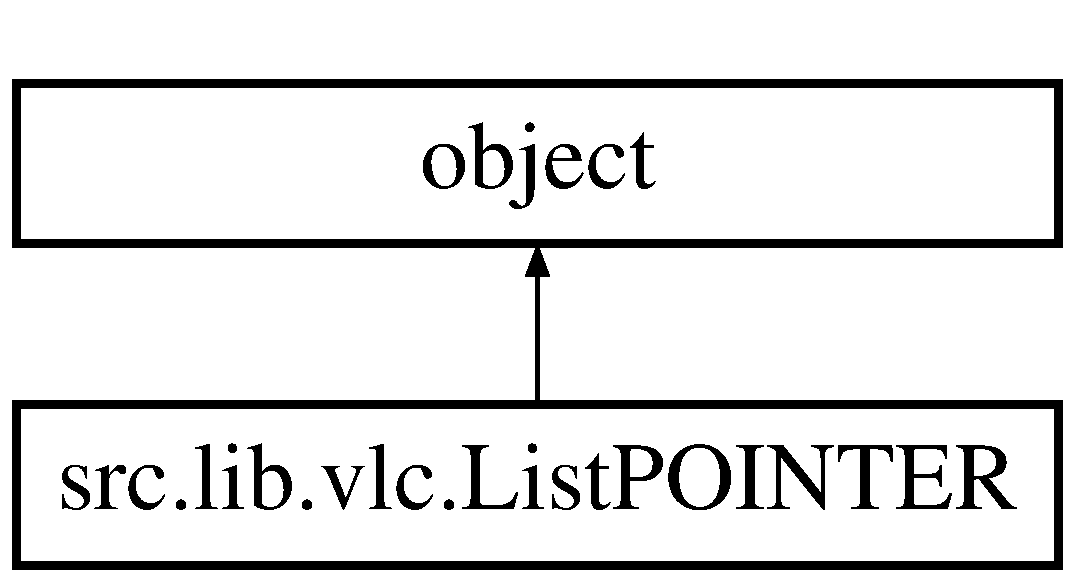
\includegraphics[height=2.000000cm]{classsrc_1_1lib_1_1vlc_1_1ListPOINTER}
\end{center}
\end{figure}
\subsection*{Public Member Functions}
\begin{DoxyCompactItemize}
\item 
def \hyperlink{classsrc_1_1lib_1_1vlc_1_1ListPOINTER_a6d646058fba287e650308951321a120e}{\+\_\+\+\_\+init\+\_\+\+\_\+} (self, \hyperlink{classsrc_1_1lib_1_1vlc_1_1ListPOINTER_a844ada7c6d6500ba23542f63587c6c32}{etype})
\item 
def \hyperlink{classsrc_1_1lib_1_1vlc_1_1ListPOINTER_a31385a500d9ca4a866d53cda05639426}{from\+\_\+param} (self, param)
\end{DoxyCompactItemize}
\subsection*{Public Attributes}
\begin{DoxyCompactItemize}
\item 
\hyperlink{classsrc_1_1lib_1_1vlc_1_1ListPOINTER_a844ada7c6d6500ba23542f63587c6c32}{etype}
\end{DoxyCompactItemize}


\subsection{Detailed Description}
\begin{DoxyVerb}Just like a POINTER but accept a list of ctype as an argument.
\end{DoxyVerb}
 

\subsection{Constructor \& Destructor Documentation}
\hypertarget{classsrc_1_1lib_1_1vlc_1_1ListPOINTER_a6d646058fba287e650308951321a120e}{}\index{src\+::lib\+::vlc\+::\+List\+P\+O\+I\+N\+T\+E\+R@{src\+::lib\+::vlc\+::\+List\+P\+O\+I\+N\+T\+E\+R}!\+\_\+\+\_\+init\+\_\+\+\_\+@{\+\_\+\+\_\+init\+\_\+\+\_\+}}
\index{\+\_\+\+\_\+init\+\_\+\+\_\+@{\+\_\+\+\_\+init\+\_\+\+\_\+}!src\+::lib\+::vlc\+::\+List\+P\+O\+I\+N\+T\+E\+R@{src\+::lib\+::vlc\+::\+List\+P\+O\+I\+N\+T\+E\+R}}
\subsubsection[{\+\_\+\+\_\+init\+\_\+\+\_\+}]{\setlength{\rightskip}{0pt plus 5cm}def src.\+lib.\+vlc.\+List\+P\+O\+I\+N\+T\+E\+R.\+\_\+\+\_\+init\+\_\+\+\_\+ (
\begin{DoxyParamCaption}
\item[{}]{self, }
\item[{}]{etype}
\end{DoxyParamCaption}
)}\label{classsrc_1_1lib_1_1vlc_1_1ListPOINTER_a6d646058fba287e650308951321a120e}


\subsection{Member Function Documentation}
\hypertarget{classsrc_1_1lib_1_1vlc_1_1ListPOINTER_a31385a500d9ca4a866d53cda05639426}{}\index{src\+::lib\+::vlc\+::\+List\+P\+O\+I\+N\+T\+E\+R@{src\+::lib\+::vlc\+::\+List\+P\+O\+I\+N\+T\+E\+R}!from\+\_\+param@{from\+\_\+param}}
\index{from\+\_\+param@{from\+\_\+param}!src\+::lib\+::vlc\+::\+List\+P\+O\+I\+N\+T\+E\+R@{src\+::lib\+::vlc\+::\+List\+P\+O\+I\+N\+T\+E\+R}}
\subsubsection[{from\+\_\+param}]{\setlength{\rightskip}{0pt plus 5cm}def src.\+lib.\+vlc.\+List\+P\+O\+I\+N\+T\+E\+R.\+from\+\_\+param (
\begin{DoxyParamCaption}
\item[{}]{self, }
\item[{}]{param}
\end{DoxyParamCaption}
)}\label{classsrc_1_1lib_1_1vlc_1_1ListPOINTER_a31385a500d9ca4a866d53cda05639426}


\subsection{Member Data Documentation}
\hypertarget{classsrc_1_1lib_1_1vlc_1_1ListPOINTER_a844ada7c6d6500ba23542f63587c6c32}{}\index{src\+::lib\+::vlc\+::\+List\+P\+O\+I\+N\+T\+E\+R@{src\+::lib\+::vlc\+::\+List\+P\+O\+I\+N\+T\+E\+R}!etype@{etype}}
\index{etype@{etype}!src\+::lib\+::vlc\+::\+List\+P\+O\+I\+N\+T\+E\+R@{src\+::lib\+::vlc\+::\+List\+P\+O\+I\+N\+T\+E\+R}}
\subsubsection[{etype}]{\setlength{\rightskip}{0pt plus 5cm}src.\+lib.\+vlc.\+List\+P\+O\+I\+N\+T\+E\+R.\+etype}\label{classsrc_1_1lib_1_1vlc_1_1ListPOINTER_a844ada7c6d6500ba23542f63587c6c32}


The documentation for this class was generated from the following file\+:\begin{DoxyCompactItemize}
\item 
src/lib/\hyperlink{vlc_8py}{vlc.\+py}\end{DoxyCompactItemize}

\hypertarget{classsrc_1_1lib_1_1vlc_1_1Log}{}\section{src.\+lib.\+vlc.\+Log Class Reference}
\label{classsrc_1_1lib_1_1vlc_1_1Log}\index{src.\+lib.\+vlc.\+Log@{src.\+lib.\+vlc.\+Log}}
Inheritance diagram for src.\+lib.\+vlc.\+Log\+:\begin{figure}[H]
\begin{center}
\leavevmode
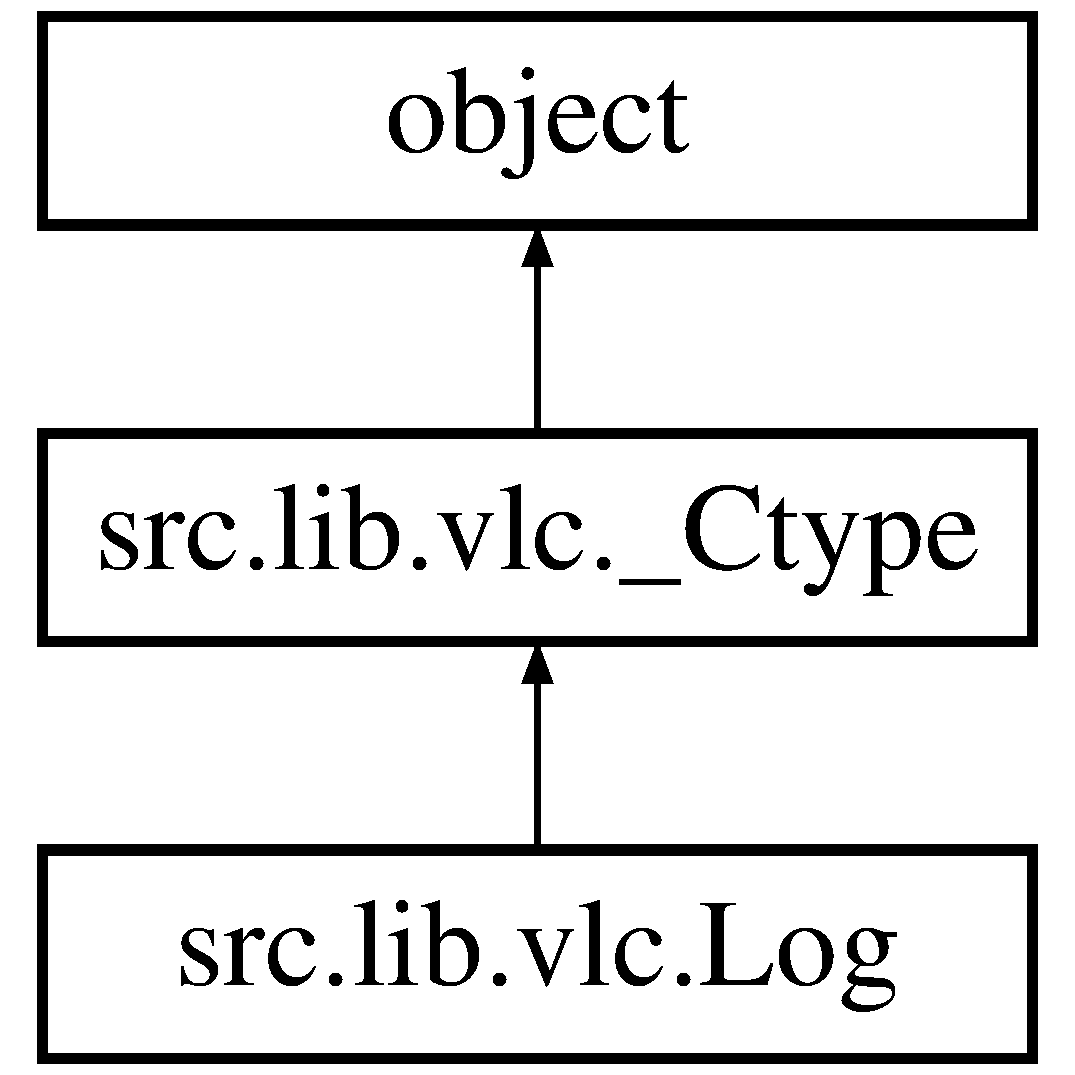
\includegraphics[height=3.000000cm]{classsrc_1_1lib_1_1vlc_1_1Log}
\end{center}
\end{figure}
\subsection*{Public Member Functions}
\begin{DoxyCompactItemize}
\item 
def \hyperlink{classsrc_1_1lib_1_1vlc_1_1Log_a40f3db8de91e4a83bdd974eddc7abc1c}{\+\_\+\+\_\+new\+\_\+\+\_\+}
\item 
def \hyperlink{classsrc_1_1lib_1_1vlc_1_1Log_a2b1193437c0b04d1ab68689276c4ad1e}{\+\_\+\+\_\+iter\+\_\+\+\_\+} (self)
\item 
def \hyperlink{classsrc_1_1lib_1_1vlc_1_1Log_a78bb207d908cf55c20d5127bf3a658ca}{dump} (self)
\item 
def \hyperlink{classsrc_1_1lib_1_1vlc_1_1Log_ad43b72a8c2fae69794b56c083474db7e}{close} (self)
\item 
def \hyperlink{classsrc_1_1lib_1_1vlc_1_1Log_a9a641ccd77e62594469d73f314a1b28f}{count} (self)
\item 
def \hyperlink{classsrc_1_1lib_1_1vlc_1_1Log_ac005bbf82dd2d3ca975655b3beedfaa8}{\+\_\+\+\_\+len\+\_\+\+\_\+} (self)
\item 
def \hyperlink{classsrc_1_1lib_1_1vlc_1_1Log_af2331b157c479853f79cccf53eeee9d6}{clear} (self)
\item 
def \hyperlink{classsrc_1_1lib_1_1vlc_1_1Log_a51708eb4df3448425cf11b6f8d010113}{get\+\_\+iterator} (self)
\end{DoxyCompactItemize}
\subsection*{Additional Inherited Members}


\subsection{Detailed Description}
\begin{DoxyVerb}Create a new VLC log instance.\end{DoxyVerb}
 

\subsection{Member Function Documentation}
\hypertarget{classsrc_1_1lib_1_1vlc_1_1Log_a2b1193437c0b04d1ab68689276c4ad1e}{}\index{src\+::lib\+::vlc\+::\+Log@{src\+::lib\+::vlc\+::\+Log}!\+\_\+\+\_\+iter\+\_\+\+\_\+@{\+\_\+\+\_\+iter\+\_\+\+\_\+}}
\index{\+\_\+\+\_\+iter\+\_\+\+\_\+@{\+\_\+\+\_\+iter\+\_\+\+\_\+}!src\+::lib\+::vlc\+::\+Log@{src\+::lib\+::vlc\+::\+Log}}
\subsubsection[{\+\_\+\+\_\+iter\+\_\+\+\_\+}]{\setlength{\rightskip}{0pt plus 5cm}def src.\+lib.\+vlc.\+Log.\+\_\+\+\_\+iter\+\_\+\+\_\+ (
\begin{DoxyParamCaption}
\item[{}]{self}
\end{DoxyParamCaption}
)}\label{classsrc_1_1lib_1_1vlc_1_1Log_a2b1193437c0b04d1ab68689276c4ad1e}
\hypertarget{classsrc_1_1lib_1_1vlc_1_1Log_ac005bbf82dd2d3ca975655b3beedfaa8}{}\index{src\+::lib\+::vlc\+::\+Log@{src\+::lib\+::vlc\+::\+Log}!\+\_\+\+\_\+len\+\_\+\+\_\+@{\+\_\+\+\_\+len\+\_\+\+\_\+}}
\index{\+\_\+\+\_\+len\+\_\+\+\_\+@{\+\_\+\+\_\+len\+\_\+\+\_\+}!src\+::lib\+::vlc\+::\+Log@{src\+::lib\+::vlc\+::\+Log}}
\subsubsection[{\+\_\+\+\_\+len\+\_\+\+\_\+}]{\setlength{\rightskip}{0pt plus 5cm}def src.\+lib.\+vlc.\+Log.\+\_\+\+\_\+len\+\_\+\+\_\+ (
\begin{DoxyParamCaption}
\item[{}]{self}
\end{DoxyParamCaption}
)}\label{classsrc_1_1lib_1_1vlc_1_1Log_ac005bbf82dd2d3ca975655b3beedfaa8}
\hypertarget{classsrc_1_1lib_1_1vlc_1_1Log_a40f3db8de91e4a83bdd974eddc7abc1c}{}\index{src\+::lib\+::vlc\+::\+Log@{src\+::lib\+::vlc\+::\+Log}!\+\_\+\+\_\+new\+\_\+\+\_\+@{\+\_\+\+\_\+new\+\_\+\+\_\+}}
\index{\+\_\+\+\_\+new\+\_\+\+\_\+@{\+\_\+\+\_\+new\+\_\+\+\_\+}!src\+::lib\+::vlc\+::\+Log@{src\+::lib\+::vlc\+::\+Log}}
\subsubsection[{\+\_\+\+\_\+new\+\_\+\+\_\+}]{\setlength{\rightskip}{0pt plus 5cm}def src.\+lib.\+vlc.\+Log.\+\_\+\+\_\+new\+\_\+\+\_\+ (
\begin{DoxyParamCaption}
\item[{}]{cls, }
\item[{}]{ptr = {\ttfamily {\bf \+\_\+internal\+\_\+guard}}}
\end{DoxyParamCaption}
)}\label{classsrc_1_1lib_1_1vlc_1_1Log_a40f3db8de91e4a83bdd974eddc7abc1c}
\begin{DoxyVerb}(INTERNAL) ctypes wrapper constructor.
\end{DoxyVerb}
 \hypertarget{classsrc_1_1lib_1_1vlc_1_1Log_af2331b157c479853f79cccf53eeee9d6}{}\index{src\+::lib\+::vlc\+::\+Log@{src\+::lib\+::vlc\+::\+Log}!clear@{clear}}
\index{clear@{clear}!src\+::lib\+::vlc\+::\+Log@{src\+::lib\+::vlc\+::\+Log}}
\subsubsection[{clear}]{\setlength{\rightskip}{0pt plus 5cm}def src.\+lib.\+vlc.\+Log.\+clear (
\begin{DoxyParamCaption}
\item[{}]{self}
\end{DoxyParamCaption}
)}\label{classsrc_1_1lib_1_1vlc_1_1Log_af2331b157c479853f79cccf53eeee9d6}
\begin{DoxyVerb}This function does nothing.
It is only provided for backward compatibility.
\end{DoxyVerb}
 \hypertarget{classsrc_1_1lib_1_1vlc_1_1Log_ad43b72a8c2fae69794b56c083474db7e}{}\index{src\+::lib\+::vlc\+::\+Log@{src\+::lib\+::vlc\+::\+Log}!close@{close}}
\index{close@{close}!src\+::lib\+::vlc\+::\+Log@{src\+::lib\+::vlc\+::\+Log}}
\subsubsection[{close}]{\setlength{\rightskip}{0pt plus 5cm}def src.\+lib.\+vlc.\+Log.\+close (
\begin{DoxyParamCaption}
\item[{}]{self}
\end{DoxyParamCaption}
)}\label{classsrc_1_1lib_1_1vlc_1_1Log_ad43b72a8c2fae69794b56c083474db7e}
\begin{DoxyVerb}Frees memory allocated by L{open}().
\end{DoxyVerb}
 \hypertarget{classsrc_1_1lib_1_1vlc_1_1Log_a9a641ccd77e62594469d73f314a1b28f}{}\index{src\+::lib\+::vlc\+::\+Log@{src\+::lib\+::vlc\+::\+Log}!count@{count}}
\index{count@{count}!src\+::lib\+::vlc\+::\+Log@{src\+::lib\+::vlc\+::\+Log}}
\subsubsection[{count}]{\setlength{\rightskip}{0pt plus 5cm}def src.\+lib.\+vlc.\+Log.\+count (
\begin{DoxyParamCaption}
\item[{}]{self}
\end{DoxyParamCaption}
)}\label{classsrc_1_1lib_1_1vlc_1_1Log_a9a641ccd77e62594469d73f314a1b28f}
\begin{DoxyVerb}Always returns zero.
This function is only provided for backward compatibility.
@return: always zero.
\end{DoxyVerb}
 \hypertarget{classsrc_1_1lib_1_1vlc_1_1Log_a78bb207d908cf55c20d5127bf3a658ca}{}\index{src\+::lib\+::vlc\+::\+Log@{src\+::lib\+::vlc\+::\+Log}!dump@{dump}}
\index{dump@{dump}!src\+::lib\+::vlc\+::\+Log@{src\+::lib\+::vlc\+::\+Log}}
\subsubsection[{dump}]{\setlength{\rightskip}{0pt plus 5cm}def src.\+lib.\+vlc.\+Log.\+dump (
\begin{DoxyParamCaption}
\item[{}]{self}
\end{DoxyParamCaption}
)}\label{classsrc_1_1lib_1_1vlc_1_1Log_a78bb207d908cf55c20d5127bf3a658ca}
\hypertarget{classsrc_1_1lib_1_1vlc_1_1Log_a51708eb4df3448425cf11b6f8d010113}{}\index{src\+::lib\+::vlc\+::\+Log@{src\+::lib\+::vlc\+::\+Log}!get\+\_\+iterator@{get\+\_\+iterator}}
\index{get\+\_\+iterator@{get\+\_\+iterator}!src\+::lib\+::vlc\+::\+Log@{src\+::lib\+::vlc\+::\+Log}}
\subsubsection[{get\+\_\+iterator}]{\setlength{\rightskip}{0pt plus 5cm}def src.\+lib.\+vlc.\+Log.\+get\+\_\+iterator (
\begin{DoxyParamCaption}
\item[{}]{self}
\end{DoxyParamCaption}
)}\label{classsrc_1_1lib_1_1vlc_1_1Log_a51708eb4df3448425cf11b6f8d010113}
\begin{DoxyVerb}This function does nothing useful.
It is only provided for backward compatibility.
@return: an unique pointer or NULL on error or if the parameter was NULL.
\end{DoxyVerb}
 

The documentation for this class was generated from the following file\+:\begin{DoxyCompactItemize}
\item 
src/lib/\hyperlink{vlc_8py}{vlc.\+py}\end{DoxyCompactItemize}

\hypertarget{classsrc_1_1lib_1_1vlc_1_1LogIterator}{}\section{src.\+lib.\+vlc.\+Log\+Iterator Class Reference}
\label{classsrc_1_1lib_1_1vlc_1_1LogIterator}\index{src.\+lib.\+vlc.\+Log\+Iterator@{src.\+lib.\+vlc.\+Log\+Iterator}}
Inheritance diagram for src.\+lib.\+vlc.\+Log\+Iterator\+:\begin{figure}[H]
\begin{center}
\leavevmode
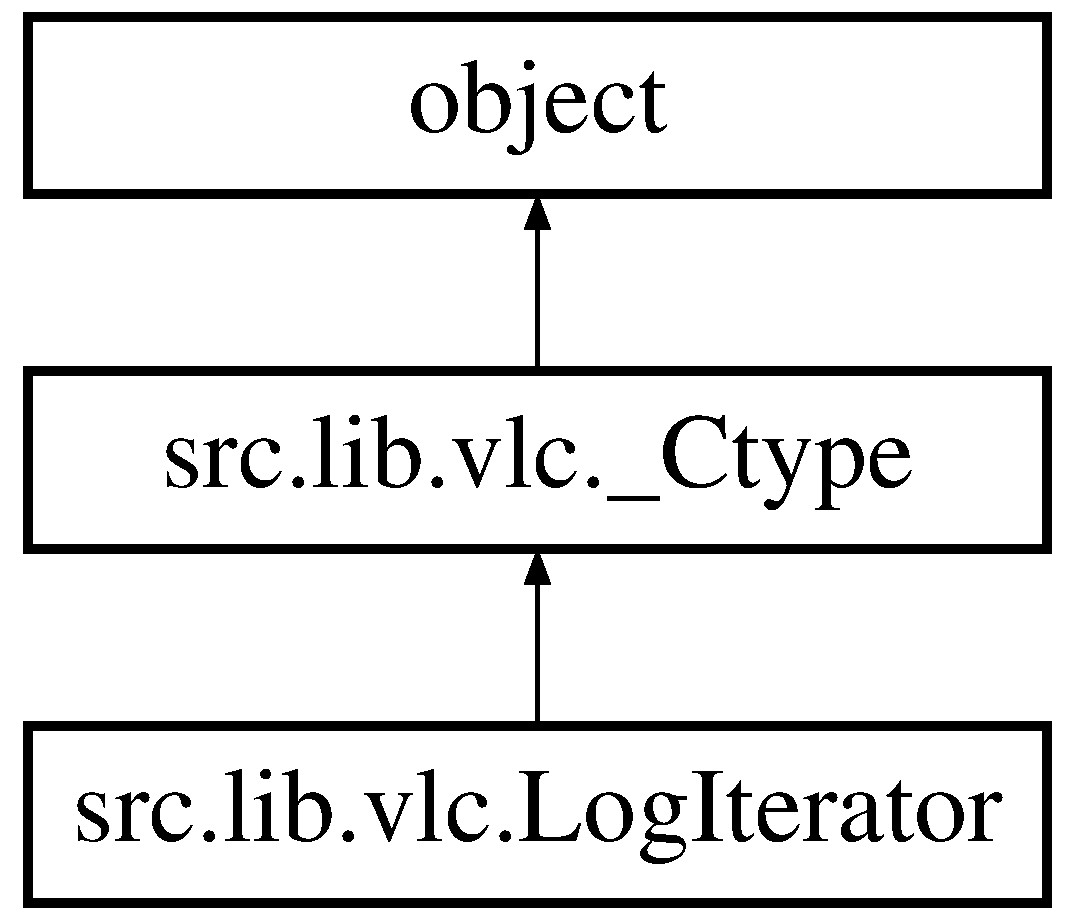
\includegraphics[height=3.000000cm]{classsrc_1_1lib_1_1vlc_1_1LogIterator}
\end{center}
\end{figure}
\subsection*{Public Member Functions}
\begin{DoxyCompactItemize}
\item 
def \hyperlink{classsrc_1_1lib_1_1vlc_1_1LogIterator_a677329352d6e6b7b7aaa9ae45ce3760c}{\+\_\+\+\_\+new\+\_\+\+\_\+}
\item 
def \hyperlink{classsrc_1_1lib_1_1vlc_1_1LogIterator_ad949350940a5bbc05804b89492998c71}{\+\_\+\+\_\+iter\+\_\+\+\_\+} (self)
\item 
def \hyperlink{classsrc_1_1lib_1_1vlc_1_1LogIterator_a5a6891f2239e340184621b51e38e3707}{next} (self)
\item 
def \hyperlink{classsrc_1_1lib_1_1vlc_1_1LogIterator_adbf4e823143e56a33abc4d022041d348}{free} (self)
\item 
def \hyperlink{classsrc_1_1lib_1_1vlc_1_1LogIterator_a158a7ceb2b29b9800200cd5a8ee4ed23}{has\+\_\+next} (self)
\end{DoxyCompactItemize}
\subsection*{Additional Inherited Members}


\subsection{Detailed Description}
\begin{DoxyVerb}Create a new VLC log iterator.\end{DoxyVerb}
 

\subsection{Member Function Documentation}
\hypertarget{classsrc_1_1lib_1_1vlc_1_1LogIterator_ad949350940a5bbc05804b89492998c71}{}\index{src\+::lib\+::vlc\+::\+Log\+Iterator@{src\+::lib\+::vlc\+::\+Log\+Iterator}!\+\_\+\+\_\+iter\+\_\+\+\_\+@{\+\_\+\+\_\+iter\+\_\+\+\_\+}}
\index{\+\_\+\+\_\+iter\+\_\+\+\_\+@{\+\_\+\+\_\+iter\+\_\+\+\_\+}!src\+::lib\+::vlc\+::\+Log\+Iterator@{src\+::lib\+::vlc\+::\+Log\+Iterator}}
\subsubsection[{\+\_\+\+\_\+iter\+\_\+\+\_\+}]{\setlength{\rightskip}{0pt plus 5cm}def src.\+lib.\+vlc.\+Log\+Iterator.\+\_\+\+\_\+iter\+\_\+\+\_\+ (
\begin{DoxyParamCaption}
\item[{}]{self}
\end{DoxyParamCaption}
)}\label{classsrc_1_1lib_1_1vlc_1_1LogIterator_ad949350940a5bbc05804b89492998c71}
\hypertarget{classsrc_1_1lib_1_1vlc_1_1LogIterator_a677329352d6e6b7b7aaa9ae45ce3760c}{}\index{src\+::lib\+::vlc\+::\+Log\+Iterator@{src\+::lib\+::vlc\+::\+Log\+Iterator}!\+\_\+\+\_\+new\+\_\+\+\_\+@{\+\_\+\+\_\+new\+\_\+\+\_\+}}
\index{\+\_\+\+\_\+new\+\_\+\+\_\+@{\+\_\+\+\_\+new\+\_\+\+\_\+}!src\+::lib\+::vlc\+::\+Log\+Iterator@{src\+::lib\+::vlc\+::\+Log\+Iterator}}
\subsubsection[{\+\_\+\+\_\+new\+\_\+\+\_\+}]{\setlength{\rightskip}{0pt plus 5cm}def src.\+lib.\+vlc.\+Log\+Iterator.\+\_\+\+\_\+new\+\_\+\+\_\+ (
\begin{DoxyParamCaption}
\item[{}]{cls, }
\item[{}]{ptr = {\ttfamily {\bf \+\_\+internal\+\_\+guard}}}
\end{DoxyParamCaption}
)}\label{classsrc_1_1lib_1_1vlc_1_1LogIterator_a677329352d6e6b7b7aaa9ae45ce3760c}
\begin{DoxyVerb}(INTERNAL) ctypes wrapper constructor.
\end{DoxyVerb}
 \hypertarget{classsrc_1_1lib_1_1vlc_1_1LogIterator_adbf4e823143e56a33abc4d022041d348}{}\index{src\+::lib\+::vlc\+::\+Log\+Iterator@{src\+::lib\+::vlc\+::\+Log\+Iterator}!free@{free}}
\index{free@{free}!src\+::lib\+::vlc\+::\+Log\+Iterator@{src\+::lib\+::vlc\+::\+Log\+Iterator}}
\subsubsection[{free}]{\setlength{\rightskip}{0pt plus 5cm}def src.\+lib.\+vlc.\+Log\+Iterator.\+free (
\begin{DoxyParamCaption}
\item[{}]{self}
\end{DoxyParamCaption}
)}\label{classsrc_1_1lib_1_1vlc_1_1LogIterator_adbf4e823143e56a33abc4d022041d348}
\begin{DoxyVerb}Frees memory allocated by L{log_get_iterator}().
\end{DoxyVerb}
 \hypertarget{classsrc_1_1lib_1_1vlc_1_1LogIterator_a158a7ceb2b29b9800200cd5a8ee4ed23}{}\index{src\+::lib\+::vlc\+::\+Log\+Iterator@{src\+::lib\+::vlc\+::\+Log\+Iterator}!has\+\_\+next@{has\+\_\+next}}
\index{has\+\_\+next@{has\+\_\+next}!src\+::lib\+::vlc\+::\+Log\+Iterator@{src\+::lib\+::vlc\+::\+Log\+Iterator}}
\subsubsection[{has\+\_\+next}]{\setlength{\rightskip}{0pt plus 5cm}def src.\+lib.\+vlc.\+Log\+Iterator.\+has\+\_\+next (
\begin{DoxyParamCaption}
\item[{}]{self}
\end{DoxyParamCaption}
)}\label{classsrc_1_1lib_1_1vlc_1_1LogIterator_a158a7ceb2b29b9800200cd5a8ee4ed23}
\begin{DoxyVerb}Always returns zero.
This function is only provided for backward compatibility.
@return: always zero.
\end{DoxyVerb}
 \hypertarget{classsrc_1_1lib_1_1vlc_1_1LogIterator_a5a6891f2239e340184621b51e38e3707}{}\index{src\+::lib\+::vlc\+::\+Log\+Iterator@{src\+::lib\+::vlc\+::\+Log\+Iterator}!next@{next}}
\index{next@{next}!src\+::lib\+::vlc\+::\+Log\+Iterator@{src\+::lib\+::vlc\+::\+Log\+Iterator}}
\subsubsection[{next}]{\setlength{\rightskip}{0pt plus 5cm}def src.\+lib.\+vlc.\+Log\+Iterator.\+next (
\begin{DoxyParamCaption}
\item[{}]{self}
\end{DoxyParamCaption}
)}\label{classsrc_1_1lib_1_1vlc_1_1LogIterator_a5a6891f2239e340184621b51e38e3707}


The documentation for this class was generated from the following file\+:\begin{DoxyCompactItemize}
\item 
src/lib/\hyperlink{vlc_8py}{vlc.\+py}\end{DoxyCompactItemize}

\hypertarget{classsrc_1_1lib_1_1vlc_1_1LogMessage}{}\section{src.\+lib.\+vlc.\+Log\+Message Class Reference}
\label{classsrc_1_1lib_1_1vlc_1_1LogMessage}\index{src.\+lib.\+vlc.\+Log\+Message@{src.\+lib.\+vlc.\+Log\+Message}}
Inheritance diagram for src.\+lib.\+vlc.\+Log\+Message\+:\begin{figure}[H]
\begin{center}
\leavevmode
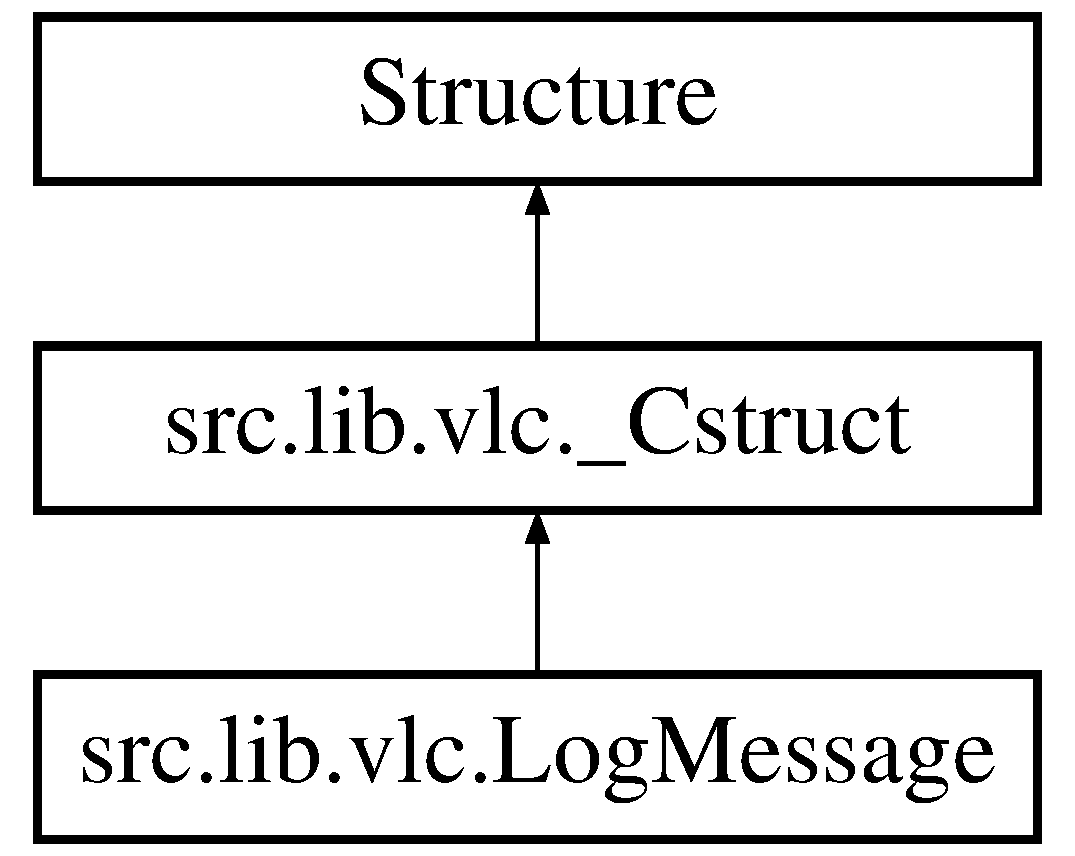
\includegraphics[height=3.000000cm]{classsrc_1_1lib_1_1vlc_1_1LogMessage}
\end{center}
\end{figure}
\subsection*{Public Member Functions}
\begin{DoxyCompactItemize}
\item 
def \hyperlink{classsrc_1_1lib_1_1vlc_1_1LogMessage_a5ec0673aa9263882a8a35845a9fb1f3b}{\+\_\+\+\_\+init\+\_\+\+\_\+} (self)
\item 
def \hyperlink{classsrc_1_1lib_1_1vlc_1_1LogMessage_a55f7184ac150ef8ed1a43742f1edaca9}{\+\_\+\+\_\+str\+\_\+\+\_\+} (self)
\end{DoxyCompactItemize}
\subsection*{Public Attributes}
\begin{DoxyCompactItemize}
\item 
\hyperlink{classsrc_1_1lib_1_1vlc_1_1LogMessage_a1be1cdb16716541b9a5a19a26072fe79}{size}
\end{DoxyCompactItemize}
\subsection*{Static Private Attributes}
\begin{DoxyCompactItemize}
\item 
list \hyperlink{classsrc_1_1lib_1_1vlc_1_1LogMessage_a030acfe26d6f47b2c5cda7e4a9f3c2eb}{\+\_\+fields\+\_\+}
\end{DoxyCompactItemize}


\subsection{Constructor \& Destructor Documentation}
\hypertarget{classsrc_1_1lib_1_1vlc_1_1LogMessage_a5ec0673aa9263882a8a35845a9fb1f3b}{}\index{src\+::lib\+::vlc\+::\+Log\+Message@{src\+::lib\+::vlc\+::\+Log\+Message}!\+\_\+\+\_\+init\+\_\+\+\_\+@{\+\_\+\+\_\+init\+\_\+\+\_\+}}
\index{\+\_\+\+\_\+init\+\_\+\+\_\+@{\+\_\+\+\_\+init\+\_\+\+\_\+}!src\+::lib\+::vlc\+::\+Log\+Message@{src\+::lib\+::vlc\+::\+Log\+Message}}
\subsubsection[{\+\_\+\+\_\+init\+\_\+\+\_\+}]{\setlength{\rightskip}{0pt plus 5cm}def src.\+lib.\+vlc.\+Log\+Message.\+\_\+\+\_\+init\+\_\+\+\_\+ (
\begin{DoxyParamCaption}
\item[{}]{self}
\end{DoxyParamCaption}
)}\label{classsrc_1_1lib_1_1vlc_1_1LogMessage_a5ec0673aa9263882a8a35845a9fb1f3b}


\subsection{Member Function Documentation}
\hypertarget{classsrc_1_1lib_1_1vlc_1_1LogMessage_a55f7184ac150ef8ed1a43742f1edaca9}{}\index{src\+::lib\+::vlc\+::\+Log\+Message@{src\+::lib\+::vlc\+::\+Log\+Message}!\+\_\+\+\_\+str\+\_\+\+\_\+@{\+\_\+\+\_\+str\+\_\+\+\_\+}}
\index{\+\_\+\+\_\+str\+\_\+\+\_\+@{\+\_\+\+\_\+str\+\_\+\+\_\+}!src\+::lib\+::vlc\+::\+Log\+Message@{src\+::lib\+::vlc\+::\+Log\+Message}}
\subsubsection[{\+\_\+\+\_\+str\+\_\+\+\_\+}]{\setlength{\rightskip}{0pt plus 5cm}def src.\+lib.\+vlc.\+Log\+Message.\+\_\+\+\_\+str\+\_\+\+\_\+ (
\begin{DoxyParamCaption}
\item[{}]{self}
\end{DoxyParamCaption}
)}\label{classsrc_1_1lib_1_1vlc_1_1LogMessage_a55f7184ac150ef8ed1a43742f1edaca9}


\subsection{Member Data Documentation}
\hypertarget{classsrc_1_1lib_1_1vlc_1_1LogMessage_a030acfe26d6f47b2c5cda7e4a9f3c2eb}{}\index{src\+::lib\+::vlc\+::\+Log\+Message@{src\+::lib\+::vlc\+::\+Log\+Message}!\+\_\+fields\+\_\+@{\+\_\+fields\+\_\+}}
\index{\+\_\+fields\+\_\+@{\+\_\+fields\+\_\+}!src\+::lib\+::vlc\+::\+Log\+Message@{src\+::lib\+::vlc\+::\+Log\+Message}}
\subsubsection[{\+\_\+fields\+\_\+}]{\setlength{\rightskip}{0pt plus 5cm}list src.\+lib.\+vlc.\+Log\+Message.\+\_\+fields\+\_\+\hspace{0.3cm}{\ttfamily [static]}, {\ttfamily [private]}}\label{classsrc_1_1lib_1_1vlc_1_1LogMessage_a030acfe26d6f47b2c5cda7e4a9f3c2eb}
{\bfseries Initial value\+:}
\begin{DoxyCode}
1 = [
2         (\textcolor{stringliteral}{'size'},     ctypes.c\_uint  ),
3         (\textcolor{stringliteral}{'severity'}, ctypes.c\_int   ),
4         (\textcolor{stringliteral}{'type'},     ctypes.c\_char\_p),
5         (\textcolor{stringliteral}{'name'},     ctypes.c\_char\_p),
6         (\textcolor{stringliteral}{'header'},   ctypes.c\_char\_p),
7         (\textcolor{stringliteral}{'message'},  ctypes.c\_char\_p),
8     ]
\end{DoxyCode}
\hypertarget{classsrc_1_1lib_1_1vlc_1_1LogMessage_a1be1cdb16716541b9a5a19a26072fe79}{}\index{src\+::lib\+::vlc\+::\+Log\+Message@{src\+::lib\+::vlc\+::\+Log\+Message}!size@{size}}
\index{size@{size}!src\+::lib\+::vlc\+::\+Log\+Message@{src\+::lib\+::vlc\+::\+Log\+Message}}
\subsubsection[{size}]{\setlength{\rightskip}{0pt plus 5cm}src.\+lib.\+vlc.\+Log\+Message.\+size}\label{classsrc_1_1lib_1_1vlc_1_1LogMessage_a1be1cdb16716541b9a5a19a26072fe79}


The documentation for this class was generated from the following file\+:\begin{DoxyCompactItemize}
\item 
src/lib/\hyperlink{vlc_8py}{vlc.\+py}\end{DoxyCompactItemize}

\hypertarget{classsrc_1_1core_1_1lossy__peer_1_1Lossy__Peer}{}\section{src.\+core.\+lossy\+\_\+peer.\+Lossy\+\_\+\+Peer Class Reference}
\label{classsrc_1_1core_1_1lossy__peer_1_1Lossy__Peer}\index{src.\+core.\+lossy\+\_\+peer.\+Lossy\+\_\+\+Peer@{src.\+core.\+lossy\+\_\+peer.\+Lossy\+\_\+\+Peer}}
Inheritance diagram for src.\+core.\+lossy\+\_\+peer.\+Lossy\+\_\+\+Peer\+:\begin{figure}[H]
\begin{center}
\leavevmode
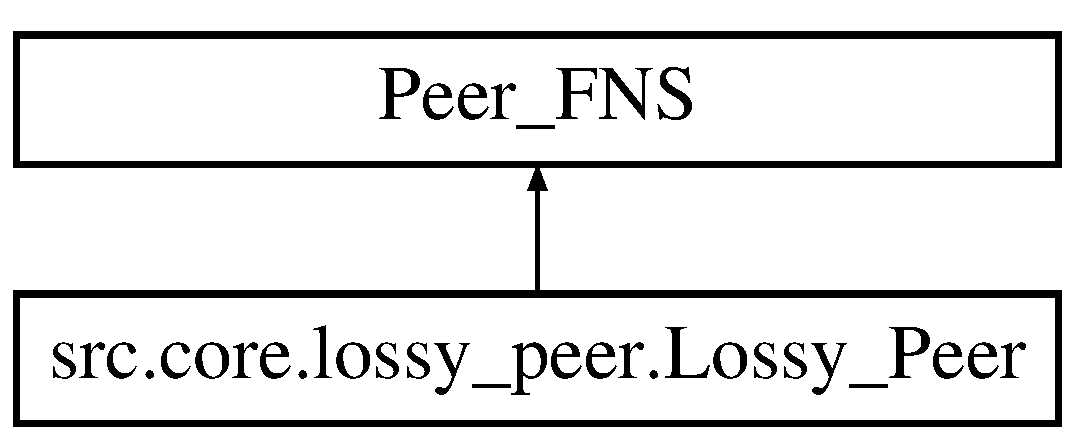
\includegraphics[height=2.000000cm]{classsrc_1_1core_1_1lossy__peer_1_1Lossy__Peer}
\end{center}
\end{figure}
\subsection*{Public Member Functions}
\begin{DoxyCompactItemize}
\item 
def \hyperlink{classsrc_1_1core_1_1lossy__peer_1_1Lossy__Peer_a3adafb293fe4d7a80955a1ee979d1ac7}{\+\_\+\+\_\+init\+\_\+\+\_\+} (self, peer)
\item 
def \hyperlink{classsrc_1_1core_1_1lossy__peer_1_1Lossy__Peer_a5ef4bd917a7e5bdcad32d44523d5345c}{print\+\_\+the\+\_\+module\+\_\+name} (self)
\item 
def \hyperlink{classsrc_1_1core_1_1lossy__peer_1_1Lossy__Peer_af4ad19b423b0dea844a2cbe6d211f0d4}{listen\+\_\+to\+\_\+the\+\_\+team} (self)
\end{DoxyCompactItemize}
\subsection*{Public Attributes}
\begin{DoxyCompactItemize}
\item 
\hyperlink{classsrc_1_1core_1_1lossy__peer_1_1Lossy__Peer_a087e9cd5f4cff34cf27e0ba681f07594}{splitter\+\_\+socket}
\item 
\hyperlink{classsrc_1_1core_1_1lossy__peer_1_1Lossy__Peer_a7bfd270bb2703665038fbf34a336db9a}{player\+\_\+socket}
\item 
\hyperlink{classsrc_1_1core_1_1lossy__peer_1_1Lossy__Peer_a1c4fe5e082d243fff4682739b1c48a76}{buffer\+\_\+size}
\item 
\hyperlink{classsrc_1_1core_1_1lossy__peer_1_1Lossy__Peer_aecdff86c33a4d0ccd46ab3170fa6e1ac}{chunk\+\_\+format\+\_\+string}
\item 
\hyperlink{classsrc_1_1core_1_1lossy__peer_1_1Lossy__Peer_a850ba6d9b1c9b3530f319a2ad70fe9f8}{splitter}
\item 
\hyperlink{classsrc_1_1core_1_1lossy__peer_1_1Lossy__Peer_a4ab6dc894a7ddc47a169b7e442ac5ddd}{chunk\+\_\+size}
\item 
\hyperlink{classsrc_1_1core_1_1lossy__peer_1_1Lossy__Peer_a784a113a40b7e2a5babd59c3330dd274}{peer\+\_\+list}
\item 
\hyperlink{classsrc_1_1core_1_1lossy__peer_1_1Lossy__Peer_adbe5a798549dfaa38eb81d1313b1216d}{debt}
\item 
\hyperlink{classsrc_1_1core_1_1lossy__peer_1_1Lossy__Peer_a3f17b1d5038ff538511b5197d6c8a22e}{team\+\_\+socket}
\end{DoxyCompactItemize}
\subsection*{Static Public Attributes}
\begin{DoxyCompactItemize}
\item 
int \hyperlink{classsrc_1_1core_1_1lossy__peer_1_1Lossy__Peer_a3afd1306f120723269df31abdcda8c56}{C\+H\+U\+N\+K\+\_\+\+L\+O\+S\+S\+\_\+\+P\+E\+R\+I\+O\+D} = 10
\end{DoxyCompactItemize}


\subsection{Constructor \& Destructor Documentation}
\hypertarget{classsrc_1_1core_1_1lossy__peer_1_1Lossy__Peer_a3adafb293fe4d7a80955a1ee979d1ac7}{}\index{src\+::core\+::lossy\+\_\+peer\+::\+Lossy\+\_\+\+Peer@{src\+::core\+::lossy\+\_\+peer\+::\+Lossy\+\_\+\+Peer}!\+\_\+\+\_\+init\+\_\+\+\_\+@{\+\_\+\+\_\+init\+\_\+\+\_\+}}
\index{\+\_\+\+\_\+init\+\_\+\+\_\+@{\+\_\+\+\_\+init\+\_\+\+\_\+}!src\+::core\+::lossy\+\_\+peer\+::\+Lossy\+\_\+\+Peer@{src\+::core\+::lossy\+\_\+peer\+::\+Lossy\+\_\+\+Peer}}
\subsubsection[{\+\_\+\+\_\+init\+\_\+\+\_\+}]{\setlength{\rightskip}{0pt plus 5cm}def src.\+core.\+lossy\+\_\+peer.\+Lossy\+\_\+\+Peer.\+\_\+\+\_\+init\+\_\+\+\_\+ (
\begin{DoxyParamCaption}
\item[{}]{self, }
\item[{}]{peer}
\end{DoxyParamCaption}
)}\label{classsrc_1_1core_1_1lossy__peer_1_1Lossy__Peer_a3adafb293fe4d7a80955a1ee979d1ac7}


\subsection{Member Function Documentation}
\hypertarget{classsrc_1_1core_1_1lossy__peer_1_1Lossy__Peer_af4ad19b423b0dea844a2cbe6d211f0d4}{}\index{src\+::core\+::lossy\+\_\+peer\+::\+Lossy\+\_\+\+Peer@{src\+::core\+::lossy\+\_\+peer\+::\+Lossy\+\_\+\+Peer}!listen\+\_\+to\+\_\+the\+\_\+team@{listen\+\_\+to\+\_\+the\+\_\+team}}
\index{listen\+\_\+to\+\_\+the\+\_\+team@{listen\+\_\+to\+\_\+the\+\_\+team}!src\+::core\+::lossy\+\_\+peer\+::\+Lossy\+\_\+\+Peer@{src\+::core\+::lossy\+\_\+peer\+::\+Lossy\+\_\+\+Peer}}
\subsubsection[{listen\+\_\+to\+\_\+the\+\_\+team}]{\setlength{\rightskip}{0pt plus 5cm}def src.\+core.\+lossy\+\_\+peer.\+Lossy\+\_\+\+Peer.\+listen\+\_\+to\+\_\+the\+\_\+team (
\begin{DoxyParamCaption}
\item[{}]{self}
\end{DoxyParamCaption}
)}\label{classsrc_1_1core_1_1lossy__peer_1_1Lossy__Peer_af4ad19b423b0dea844a2cbe6d211f0d4}
\hypertarget{classsrc_1_1core_1_1lossy__peer_1_1Lossy__Peer_a5ef4bd917a7e5bdcad32d44523d5345c}{}\index{src\+::core\+::lossy\+\_\+peer\+::\+Lossy\+\_\+\+Peer@{src\+::core\+::lossy\+\_\+peer\+::\+Lossy\+\_\+\+Peer}!print\+\_\+the\+\_\+module\+\_\+name@{print\+\_\+the\+\_\+module\+\_\+name}}
\index{print\+\_\+the\+\_\+module\+\_\+name@{print\+\_\+the\+\_\+module\+\_\+name}!src\+::core\+::lossy\+\_\+peer\+::\+Lossy\+\_\+\+Peer@{src\+::core\+::lossy\+\_\+peer\+::\+Lossy\+\_\+\+Peer}}
\subsubsection[{print\+\_\+the\+\_\+module\+\_\+name}]{\setlength{\rightskip}{0pt plus 5cm}def src.\+core.\+lossy\+\_\+peer.\+Lossy\+\_\+\+Peer.\+print\+\_\+the\+\_\+module\+\_\+name (
\begin{DoxyParamCaption}
\item[{}]{self}
\end{DoxyParamCaption}
)}\label{classsrc_1_1core_1_1lossy__peer_1_1Lossy__Peer_a5ef4bd917a7e5bdcad32d44523d5345c}


\subsection{Member Data Documentation}
\hypertarget{classsrc_1_1core_1_1lossy__peer_1_1Lossy__Peer_a1c4fe5e082d243fff4682739b1c48a76}{}\index{src\+::core\+::lossy\+\_\+peer\+::\+Lossy\+\_\+\+Peer@{src\+::core\+::lossy\+\_\+peer\+::\+Lossy\+\_\+\+Peer}!buffer\+\_\+size@{buffer\+\_\+size}}
\index{buffer\+\_\+size@{buffer\+\_\+size}!src\+::core\+::lossy\+\_\+peer\+::\+Lossy\+\_\+\+Peer@{src\+::core\+::lossy\+\_\+peer\+::\+Lossy\+\_\+\+Peer}}
\subsubsection[{buffer\+\_\+size}]{\setlength{\rightskip}{0pt plus 5cm}src.\+core.\+lossy\+\_\+peer.\+Lossy\+\_\+\+Peer.\+buffer\+\_\+size}\label{classsrc_1_1core_1_1lossy__peer_1_1Lossy__Peer_a1c4fe5e082d243fff4682739b1c48a76}
\hypertarget{classsrc_1_1core_1_1lossy__peer_1_1Lossy__Peer_aecdff86c33a4d0ccd46ab3170fa6e1ac}{}\index{src\+::core\+::lossy\+\_\+peer\+::\+Lossy\+\_\+\+Peer@{src\+::core\+::lossy\+\_\+peer\+::\+Lossy\+\_\+\+Peer}!chunk\+\_\+format\+\_\+string@{chunk\+\_\+format\+\_\+string}}
\index{chunk\+\_\+format\+\_\+string@{chunk\+\_\+format\+\_\+string}!src\+::core\+::lossy\+\_\+peer\+::\+Lossy\+\_\+\+Peer@{src\+::core\+::lossy\+\_\+peer\+::\+Lossy\+\_\+\+Peer}}
\subsubsection[{chunk\+\_\+format\+\_\+string}]{\setlength{\rightskip}{0pt plus 5cm}src.\+core.\+lossy\+\_\+peer.\+Lossy\+\_\+\+Peer.\+chunk\+\_\+format\+\_\+string}\label{classsrc_1_1core_1_1lossy__peer_1_1Lossy__Peer_aecdff86c33a4d0ccd46ab3170fa6e1ac}
\hypertarget{classsrc_1_1core_1_1lossy__peer_1_1Lossy__Peer_a3afd1306f120723269df31abdcda8c56}{}\index{src\+::core\+::lossy\+\_\+peer\+::\+Lossy\+\_\+\+Peer@{src\+::core\+::lossy\+\_\+peer\+::\+Lossy\+\_\+\+Peer}!C\+H\+U\+N\+K\+\_\+\+L\+O\+S\+S\+\_\+\+P\+E\+R\+I\+O\+D@{C\+H\+U\+N\+K\+\_\+\+L\+O\+S\+S\+\_\+\+P\+E\+R\+I\+O\+D}}
\index{C\+H\+U\+N\+K\+\_\+\+L\+O\+S\+S\+\_\+\+P\+E\+R\+I\+O\+D@{C\+H\+U\+N\+K\+\_\+\+L\+O\+S\+S\+\_\+\+P\+E\+R\+I\+O\+D}!src\+::core\+::lossy\+\_\+peer\+::\+Lossy\+\_\+\+Peer@{src\+::core\+::lossy\+\_\+peer\+::\+Lossy\+\_\+\+Peer}}
\subsubsection[{C\+H\+U\+N\+K\+\_\+\+L\+O\+S\+S\+\_\+\+P\+E\+R\+I\+O\+D}]{\setlength{\rightskip}{0pt plus 5cm}int src.\+core.\+lossy\+\_\+peer.\+Lossy\+\_\+\+Peer.\+C\+H\+U\+N\+K\+\_\+\+L\+O\+S\+S\+\_\+\+P\+E\+R\+I\+O\+D = 10\hspace{0.3cm}{\ttfamily [static]}}\label{classsrc_1_1core_1_1lossy__peer_1_1Lossy__Peer_a3afd1306f120723269df31abdcda8c56}
\hypertarget{classsrc_1_1core_1_1lossy__peer_1_1Lossy__Peer_a4ab6dc894a7ddc47a169b7e442ac5ddd}{}\index{src\+::core\+::lossy\+\_\+peer\+::\+Lossy\+\_\+\+Peer@{src\+::core\+::lossy\+\_\+peer\+::\+Lossy\+\_\+\+Peer}!chunk\+\_\+size@{chunk\+\_\+size}}
\index{chunk\+\_\+size@{chunk\+\_\+size}!src\+::core\+::lossy\+\_\+peer\+::\+Lossy\+\_\+\+Peer@{src\+::core\+::lossy\+\_\+peer\+::\+Lossy\+\_\+\+Peer}}
\subsubsection[{chunk\+\_\+size}]{\setlength{\rightskip}{0pt plus 5cm}src.\+core.\+lossy\+\_\+peer.\+Lossy\+\_\+\+Peer.\+chunk\+\_\+size}\label{classsrc_1_1core_1_1lossy__peer_1_1Lossy__Peer_a4ab6dc894a7ddc47a169b7e442ac5ddd}
\hypertarget{classsrc_1_1core_1_1lossy__peer_1_1Lossy__Peer_adbe5a798549dfaa38eb81d1313b1216d}{}\index{src\+::core\+::lossy\+\_\+peer\+::\+Lossy\+\_\+\+Peer@{src\+::core\+::lossy\+\_\+peer\+::\+Lossy\+\_\+\+Peer}!debt@{debt}}
\index{debt@{debt}!src\+::core\+::lossy\+\_\+peer\+::\+Lossy\+\_\+\+Peer@{src\+::core\+::lossy\+\_\+peer\+::\+Lossy\+\_\+\+Peer}}
\subsubsection[{debt}]{\setlength{\rightskip}{0pt plus 5cm}src.\+core.\+lossy\+\_\+peer.\+Lossy\+\_\+\+Peer.\+debt}\label{classsrc_1_1core_1_1lossy__peer_1_1Lossy__Peer_adbe5a798549dfaa38eb81d1313b1216d}
\hypertarget{classsrc_1_1core_1_1lossy__peer_1_1Lossy__Peer_a784a113a40b7e2a5babd59c3330dd274}{}\index{src\+::core\+::lossy\+\_\+peer\+::\+Lossy\+\_\+\+Peer@{src\+::core\+::lossy\+\_\+peer\+::\+Lossy\+\_\+\+Peer}!peer\+\_\+list@{peer\+\_\+list}}
\index{peer\+\_\+list@{peer\+\_\+list}!src\+::core\+::lossy\+\_\+peer\+::\+Lossy\+\_\+\+Peer@{src\+::core\+::lossy\+\_\+peer\+::\+Lossy\+\_\+\+Peer}}
\subsubsection[{peer\+\_\+list}]{\setlength{\rightskip}{0pt plus 5cm}src.\+core.\+lossy\+\_\+peer.\+Lossy\+\_\+\+Peer.\+peer\+\_\+list}\label{classsrc_1_1core_1_1lossy__peer_1_1Lossy__Peer_a784a113a40b7e2a5babd59c3330dd274}
\hypertarget{classsrc_1_1core_1_1lossy__peer_1_1Lossy__Peer_a7bfd270bb2703665038fbf34a336db9a}{}\index{src\+::core\+::lossy\+\_\+peer\+::\+Lossy\+\_\+\+Peer@{src\+::core\+::lossy\+\_\+peer\+::\+Lossy\+\_\+\+Peer}!player\+\_\+socket@{player\+\_\+socket}}
\index{player\+\_\+socket@{player\+\_\+socket}!src\+::core\+::lossy\+\_\+peer\+::\+Lossy\+\_\+\+Peer@{src\+::core\+::lossy\+\_\+peer\+::\+Lossy\+\_\+\+Peer}}
\subsubsection[{player\+\_\+socket}]{\setlength{\rightskip}{0pt plus 5cm}src.\+core.\+lossy\+\_\+peer.\+Lossy\+\_\+\+Peer.\+player\+\_\+socket}\label{classsrc_1_1core_1_1lossy__peer_1_1Lossy__Peer_a7bfd270bb2703665038fbf34a336db9a}
\hypertarget{classsrc_1_1core_1_1lossy__peer_1_1Lossy__Peer_a850ba6d9b1c9b3530f319a2ad70fe9f8}{}\index{src\+::core\+::lossy\+\_\+peer\+::\+Lossy\+\_\+\+Peer@{src\+::core\+::lossy\+\_\+peer\+::\+Lossy\+\_\+\+Peer}!splitter@{splitter}}
\index{splitter@{splitter}!src\+::core\+::lossy\+\_\+peer\+::\+Lossy\+\_\+\+Peer@{src\+::core\+::lossy\+\_\+peer\+::\+Lossy\+\_\+\+Peer}}
\subsubsection[{splitter}]{\setlength{\rightskip}{0pt plus 5cm}src.\+core.\+lossy\+\_\+peer.\+Lossy\+\_\+\+Peer.\+splitter}\label{classsrc_1_1core_1_1lossy__peer_1_1Lossy__Peer_a850ba6d9b1c9b3530f319a2ad70fe9f8}
\hypertarget{classsrc_1_1core_1_1lossy__peer_1_1Lossy__Peer_a087e9cd5f4cff34cf27e0ba681f07594}{}\index{src\+::core\+::lossy\+\_\+peer\+::\+Lossy\+\_\+\+Peer@{src\+::core\+::lossy\+\_\+peer\+::\+Lossy\+\_\+\+Peer}!splitter\+\_\+socket@{splitter\+\_\+socket}}
\index{splitter\+\_\+socket@{splitter\+\_\+socket}!src\+::core\+::lossy\+\_\+peer\+::\+Lossy\+\_\+\+Peer@{src\+::core\+::lossy\+\_\+peer\+::\+Lossy\+\_\+\+Peer}}
\subsubsection[{splitter\+\_\+socket}]{\setlength{\rightskip}{0pt plus 5cm}src.\+core.\+lossy\+\_\+peer.\+Lossy\+\_\+\+Peer.\+splitter\+\_\+socket}\label{classsrc_1_1core_1_1lossy__peer_1_1Lossy__Peer_a087e9cd5f4cff34cf27e0ba681f07594}
\hypertarget{classsrc_1_1core_1_1lossy__peer_1_1Lossy__Peer_a3f17b1d5038ff538511b5197d6c8a22e}{}\index{src\+::core\+::lossy\+\_\+peer\+::\+Lossy\+\_\+\+Peer@{src\+::core\+::lossy\+\_\+peer\+::\+Lossy\+\_\+\+Peer}!team\+\_\+socket@{team\+\_\+socket}}
\index{team\+\_\+socket@{team\+\_\+socket}!src\+::core\+::lossy\+\_\+peer\+::\+Lossy\+\_\+\+Peer@{src\+::core\+::lossy\+\_\+peer\+::\+Lossy\+\_\+\+Peer}}
\subsubsection[{team\+\_\+socket}]{\setlength{\rightskip}{0pt plus 5cm}src.\+core.\+lossy\+\_\+peer.\+Lossy\+\_\+\+Peer.\+team\+\_\+socket}\label{classsrc_1_1core_1_1lossy__peer_1_1Lossy__Peer_a3f17b1d5038ff538511b5197d6c8a22e}


The documentation for this class was generated from the following file\+:\begin{DoxyCompactItemize}
\item 
src/core/\hyperlink{lossy__peer_8py}{lossy\+\_\+peer.\+py}\end{DoxyCompactItemize}

\hypertarget{classsrc_1_1core_1_1lossy__socket_1_1lossy__socket}{}\section{src.\+core.\+lossy\+\_\+socket.\+lossy\+\_\+socket Class Reference}
\label{classsrc_1_1core_1_1lossy__socket_1_1lossy__socket}\index{src.\+core.\+lossy\+\_\+socket.\+lossy\+\_\+socket@{src.\+core.\+lossy\+\_\+socket.\+lossy\+\_\+socket}}
\subsection*{Public Member Functions}
\begin{DoxyCompactItemize}
\item 
def \hyperlink{classsrc_1_1core_1_1lossy__socket_1_1lossy__socket_acdb17e6fe730ee39b3ecbe9a223a0f13}{\+\_\+\+\_\+init\+\_\+\+\_\+} (self, \hyperlink{classsrc_1_1core_1_1lossy__socket_1_1lossy__socket_a81b0908197756019eed96bdefbd2318a}{ratio}, p)
\item 
def \hyperlink{classsrc_1_1core_1_1lossy__socket_1_1lossy__socket_ad2847304d2d79d21379c7761b455a248}{sendto} (self, p)
\item 
def \hyperlink{classsrc_1_1core_1_1lossy__socket_1_1lossy__socket_a669395beafad2d3f3268d7b5b8f10d0c}{bind} (self, p)
\item 
def \hyperlink{classsrc_1_1core_1_1lossy__socket_1_1lossy__socket_a4c3abab9c140d0ad8cbcdff130c0aed3}{settimeout} (self, p)
\item 
def \hyperlink{classsrc_1_1core_1_1lossy__socket_1_1lossy__socket_aca63fd75c31bf2388b554fda27bfa0ad}{getsockname} (self, p)
\item 
def \hyperlink{classsrc_1_1core_1_1lossy__socket_1_1lossy__socket_a62eaa5c0db5b03b207c536014c454bed}{recvfrom} (self, p)
\item 
def \hyperlink{classsrc_1_1core_1_1lossy__socket_1_1lossy__socket_a37805321d148b23439497c7155bf0821}{setsockopt} (self, p)
\end{DoxyCompactItemize}
\subsection*{Public Attributes}
\begin{DoxyCompactItemize}
\item 
\hyperlink{classsrc_1_1core_1_1lossy__socket_1_1lossy__socket_a547f97977756be02b80d81b6293804fa}{counter}
\item 
\hyperlink{classsrc_1_1core_1_1lossy__socket_1_1lossy__socket_a81b0908197756019eed96bdefbd2318a}{ratio}
\end{DoxyCompactItemize}
\subsection*{Private Attributes}
\begin{DoxyCompactItemize}
\item 
\hyperlink{classsrc_1_1core_1_1lossy__socket_1_1lossy__socket_a2826b858da17656697d98727c53991a0}{\+\_\+sock}
\end{DoxyCompactItemize}


\subsection{Constructor \& Destructor Documentation}
\hypertarget{classsrc_1_1core_1_1lossy__socket_1_1lossy__socket_acdb17e6fe730ee39b3ecbe9a223a0f13}{}\index{src\+::core\+::lossy\+\_\+socket\+::lossy\+\_\+socket@{src\+::core\+::lossy\+\_\+socket\+::lossy\+\_\+socket}!\+\_\+\+\_\+init\+\_\+\+\_\+@{\+\_\+\+\_\+init\+\_\+\+\_\+}}
\index{\+\_\+\+\_\+init\+\_\+\+\_\+@{\+\_\+\+\_\+init\+\_\+\+\_\+}!src\+::core\+::lossy\+\_\+socket\+::lossy\+\_\+socket@{src\+::core\+::lossy\+\_\+socket\+::lossy\+\_\+socket}}
\subsubsection[{\+\_\+\+\_\+init\+\_\+\+\_\+}]{\setlength{\rightskip}{0pt plus 5cm}def src.\+core.\+lossy\+\_\+socket.\+lossy\+\_\+socket.\+\_\+\+\_\+init\+\_\+\+\_\+ (
\begin{DoxyParamCaption}
\item[{}]{self, }
\item[{}]{ratio, }
\item[{}]{p}
\end{DoxyParamCaption}
)}\label{classsrc_1_1core_1_1lossy__socket_1_1lossy__socket_acdb17e6fe730ee39b3ecbe9a223a0f13}


\subsection{Member Function Documentation}
\hypertarget{classsrc_1_1core_1_1lossy__socket_1_1lossy__socket_a669395beafad2d3f3268d7b5b8f10d0c}{}\index{src\+::core\+::lossy\+\_\+socket\+::lossy\+\_\+socket@{src\+::core\+::lossy\+\_\+socket\+::lossy\+\_\+socket}!bind@{bind}}
\index{bind@{bind}!src\+::core\+::lossy\+\_\+socket\+::lossy\+\_\+socket@{src\+::core\+::lossy\+\_\+socket\+::lossy\+\_\+socket}}
\subsubsection[{bind}]{\setlength{\rightskip}{0pt plus 5cm}def src.\+core.\+lossy\+\_\+socket.\+lossy\+\_\+socket.\+bind (
\begin{DoxyParamCaption}
\item[{}]{self, }
\item[{}]{p}
\end{DoxyParamCaption}
)}\label{classsrc_1_1core_1_1lossy__socket_1_1lossy__socket_a669395beafad2d3f3268d7b5b8f10d0c}
\hypertarget{classsrc_1_1core_1_1lossy__socket_1_1lossy__socket_aca63fd75c31bf2388b554fda27bfa0ad}{}\index{src\+::core\+::lossy\+\_\+socket\+::lossy\+\_\+socket@{src\+::core\+::lossy\+\_\+socket\+::lossy\+\_\+socket}!getsockname@{getsockname}}
\index{getsockname@{getsockname}!src\+::core\+::lossy\+\_\+socket\+::lossy\+\_\+socket@{src\+::core\+::lossy\+\_\+socket\+::lossy\+\_\+socket}}
\subsubsection[{getsockname}]{\setlength{\rightskip}{0pt plus 5cm}def src.\+core.\+lossy\+\_\+socket.\+lossy\+\_\+socket.\+getsockname (
\begin{DoxyParamCaption}
\item[{}]{self, }
\item[{}]{p}
\end{DoxyParamCaption}
)}\label{classsrc_1_1core_1_1lossy__socket_1_1lossy__socket_aca63fd75c31bf2388b554fda27bfa0ad}
\hypertarget{classsrc_1_1core_1_1lossy__socket_1_1lossy__socket_a62eaa5c0db5b03b207c536014c454bed}{}\index{src\+::core\+::lossy\+\_\+socket\+::lossy\+\_\+socket@{src\+::core\+::lossy\+\_\+socket\+::lossy\+\_\+socket}!recvfrom@{recvfrom}}
\index{recvfrom@{recvfrom}!src\+::core\+::lossy\+\_\+socket\+::lossy\+\_\+socket@{src\+::core\+::lossy\+\_\+socket\+::lossy\+\_\+socket}}
\subsubsection[{recvfrom}]{\setlength{\rightskip}{0pt plus 5cm}def src.\+core.\+lossy\+\_\+socket.\+lossy\+\_\+socket.\+recvfrom (
\begin{DoxyParamCaption}
\item[{}]{self, }
\item[{}]{p}
\end{DoxyParamCaption}
)}\label{classsrc_1_1core_1_1lossy__socket_1_1lossy__socket_a62eaa5c0db5b03b207c536014c454bed}
\hypertarget{classsrc_1_1core_1_1lossy__socket_1_1lossy__socket_ad2847304d2d79d21379c7761b455a248}{}\index{src\+::core\+::lossy\+\_\+socket\+::lossy\+\_\+socket@{src\+::core\+::lossy\+\_\+socket\+::lossy\+\_\+socket}!sendto@{sendto}}
\index{sendto@{sendto}!src\+::core\+::lossy\+\_\+socket\+::lossy\+\_\+socket@{src\+::core\+::lossy\+\_\+socket\+::lossy\+\_\+socket}}
\subsubsection[{sendto}]{\setlength{\rightskip}{0pt plus 5cm}def src.\+core.\+lossy\+\_\+socket.\+lossy\+\_\+socket.\+sendto (
\begin{DoxyParamCaption}
\item[{}]{self, }
\item[{}]{p}
\end{DoxyParamCaption}
)}\label{classsrc_1_1core_1_1lossy__socket_1_1lossy__socket_ad2847304d2d79d21379c7761b455a248}
\hypertarget{classsrc_1_1core_1_1lossy__socket_1_1lossy__socket_a37805321d148b23439497c7155bf0821}{}\index{src\+::core\+::lossy\+\_\+socket\+::lossy\+\_\+socket@{src\+::core\+::lossy\+\_\+socket\+::lossy\+\_\+socket}!setsockopt@{setsockopt}}
\index{setsockopt@{setsockopt}!src\+::core\+::lossy\+\_\+socket\+::lossy\+\_\+socket@{src\+::core\+::lossy\+\_\+socket\+::lossy\+\_\+socket}}
\subsubsection[{setsockopt}]{\setlength{\rightskip}{0pt plus 5cm}def src.\+core.\+lossy\+\_\+socket.\+lossy\+\_\+socket.\+setsockopt (
\begin{DoxyParamCaption}
\item[{}]{self, }
\item[{}]{p}
\end{DoxyParamCaption}
)}\label{classsrc_1_1core_1_1lossy__socket_1_1lossy__socket_a37805321d148b23439497c7155bf0821}
\hypertarget{classsrc_1_1core_1_1lossy__socket_1_1lossy__socket_a4c3abab9c140d0ad8cbcdff130c0aed3}{}\index{src\+::core\+::lossy\+\_\+socket\+::lossy\+\_\+socket@{src\+::core\+::lossy\+\_\+socket\+::lossy\+\_\+socket}!settimeout@{settimeout}}
\index{settimeout@{settimeout}!src\+::core\+::lossy\+\_\+socket\+::lossy\+\_\+socket@{src\+::core\+::lossy\+\_\+socket\+::lossy\+\_\+socket}}
\subsubsection[{settimeout}]{\setlength{\rightskip}{0pt plus 5cm}def src.\+core.\+lossy\+\_\+socket.\+lossy\+\_\+socket.\+settimeout (
\begin{DoxyParamCaption}
\item[{}]{self, }
\item[{}]{p}
\end{DoxyParamCaption}
)}\label{classsrc_1_1core_1_1lossy__socket_1_1lossy__socket_a4c3abab9c140d0ad8cbcdff130c0aed3}


\subsection{Member Data Documentation}
\hypertarget{classsrc_1_1core_1_1lossy__socket_1_1lossy__socket_a2826b858da17656697d98727c53991a0}{}\index{src\+::core\+::lossy\+\_\+socket\+::lossy\+\_\+socket@{src\+::core\+::lossy\+\_\+socket\+::lossy\+\_\+socket}!\+\_\+sock@{\+\_\+sock}}
\index{\+\_\+sock@{\+\_\+sock}!src\+::core\+::lossy\+\_\+socket\+::lossy\+\_\+socket@{src\+::core\+::lossy\+\_\+socket\+::lossy\+\_\+socket}}
\subsubsection[{\+\_\+sock}]{\setlength{\rightskip}{0pt plus 5cm}src.\+core.\+lossy\+\_\+socket.\+lossy\+\_\+socket.\+\_\+sock\hspace{0.3cm}{\ttfamily [private]}}\label{classsrc_1_1core_1_1lossy__socket_1_1lossy__socket_a2826b858da17656697d98727c53991a0}
\hypertarget{classsrc_1_1core_1_1lossy__socket_1_1lossy__socket_a547f97977756be02b80d81b6293804fa}{}\index{src\+::core\+::lossy\+\_\+socket\+::lossy\+\_\+socket@{src\+::core\+::lossy\+\_\+socket\+::lossy\+\_\+socket}!counter@{counter}}
\index{counter@{counter}!src\+::core\+::lossy\+\_\+socket\+::lossy\+\_\+socket@{src\+::core\+::lossy\+\_\+socket\+::lossy\+\_\+socket}}
\subsubsection[{counter}]{\setlength{\rightskip}{0pt plus 5cm}src.\+core.\+lossy\+\_\+socket.\+lossy\+\_\+socket.\+counter}\label{classsrc_1_1core_1_1lossy__socket_1_1lossy__socket_a547f97977756be02b80d81b6293804fa}
\hypertarget{classsrc_1_1core_1_1lossy__socket_1_1lossy__socket_a81b0908197756019eed96bdefbd2318a}{}\index{src\+::core\+::lossy\+\_\+socket\+::lossy\+\_\+socket@{src\+::core\+::lossy\+\_\+socket\+::lossy\+\_\+socket}!ratio@{ratio}}
\index{ratio@{ratio}!src\+::core\+::lossy\+\_\+socket\+::lossy\+\_\+socket@{src\+::core\+::lossy\+\_\+socket\+::lossy\+\_\+socket}}
\subsubsection[{ratio}]{\setlength{\rightskip}{0pt plus 5cm}src.\+core.\+lossy\+\_\+socket.\+lossy\+\_\+socket.\+ratio}\label{classsrc_1_1core_1_1lossy__socket_1_1lossy__socket_a81b0908197756019eed96bdefbd2318a}


The documentation for this class was generated from the following file\+:\begin{DoxyCompactItemize}
\item 
src/core/\hyperlink{lossy__socket_8py}{lossy\+\_\+socket.\+py}\end{DoxyCompactItemize}

\hypertarget{classsrc_1_1controller_1_1main__window__controller_1_1Main__Controller}{}\section{src.\+controller.\+main\+\_\+window\+\_\+controller.\+Main\+\_\+\+Controller Class Reference}
\label{classsrc_1_1controller_1_1main__window__controller_1_1Main__Controller}\index{src.\+controller.\+main\+\_\+window\+\_\+controller.\+Main\+\_\+\+Controller@{src.\+controller.\+main\+\_\+window\+\_\+controller.\+Main\+\_\+\+Controller}}
\subsection*{Public Member Functions}
\begin{DoxyCompactItemize}
\item 
def \hyperlink{classsrc_1_1controller_1_1main__window__controller_1_1Main__Controller_a52d7589f44db394016d96c594f5cecdd}{\+\_\+\+\_\+init\+\_\+\+\_\+} (self, window, model)
\item 
def \hyperlink{classsrc_1_1controller_1_1main__window__controller_1_1Main__Controller_a1fa29af8cfb2631e8cf8800be1b7f178}{export\+\_\+sample\+\_\+monitor} (self)
\item 
def \hyperlink{classsrc_1_1controller_1_1main__window__controller_1_1Main__Controller_a189d0d3e9985f5eb749673e90f37a3ee}{show\+\_\+monitor\+\_\+channel} (self)
\item 
def \hyperlink{classsrc_1_1controller_1_1main__window__controller_1_1Main__Controller_ab7264805bcee4ecf770fc38bf788949d}{start\+\_\+peer} (self)
\item 
def \hyperlink{classsrc_1_1controller_1_1main__window__controller_1_1Main__Controller_a27fb26c5e650e47052c4ef26bc6efc03}{show} (self)
\item 
def \hyperlink{classsrc_1_1controller_1_1main__window__controller_1_1Main__Controller_ad044b9b8e5113bebd642ad605bf52fc2}{setup\+\_\+signals} (self)
\item 
def \hyperlink{classsrc_1_1controller_1_1main__window__controller_1_1Main__Controller_a1726bd2bbc6ed953237d8c590051d6d8}{import\+\_\+channels}
\item 
def \hyperlink{classsrc_1_1controller_1_1main__window__controller_1_1Main__Controller_a0354392bbaa3516eb03a3ad69981054d}{export\+\_\+channels}
\item 
def \hyperlink{classsrc_1_1controller_1_1main__window__controller_1_1Main__Controller_a261d6830a754581570c4f6dd7407d1a8}{toggle\+\_\+player\+\_\+type} (self, \hyperlink{classsrc_1_1controller_1_1main__window__controller_1_1Main__Controller_ad15c49dcab2e7227f2708e253aedebe9}{win\+\_\+id})
\item 
def \hyperlink{classsrc_1_1controller_1_1main__window__controller_1_1Main__Controller_aedf99574bc601bb0dd9c94b7bce8caf8}{stop\+\_\+player}
\item 
def \hyperlink{classsrc_1_1controller_1_1main__window__controller_1_1Main__Controller_a06983af1c97e7a65d017a874ec4b7611}{quit} (self)
\item 
def \hyperlink{classsrc_1_1controller_1_1main__window__controller_1_1Main__Controller_a54109148c910bc97c8627b8015c93e54}{end\+\_\+callback} (self)
\item 
def \hyperlink{classsrc_1_1controller_1_1main__window__controller_1_1Main__Controller_a659a847cea22c0f009f7159d3cede066}{toggle\+\_\+player\+\_\+playback}
\item 
def \hyperlink{classsrc_1_1controller_1_1main__window__controller_1_1Main__Controller_a4985d9f75fefa2bbe1dd9634ca732307}{toggle\+\_\+channel\+\_\+box}
\item 
def \hyperlink{classsrc_1_1controller_1_1main__window__controller_1_1Main__Controller_a62875a0cdef59b879b1327123c4bf19b}{toggle\+\_\+player\+\_\+fullscreen}
\item 
def \hyperlink{classsrc_1_1controller_1_1main__window__controller_1_1Main__Controller_a8b3a8591b3f21e8b27367f507a17d67d}{redraw\+\_\+surface}
\item 
def \hyperlink{classsrc_1_1controller_1_1main__window__controller_1_1Main__Controller_acd7580c588a663d3c486ac21c7d37c24}{toggle\+\_\+status\+\_\+box}
\item 
def \hyperlink{classsrc_1_1controller_1_1main__window__controller_1_1Main__Controller_ab76be820cb4c56971e732bfc761cc7b3}{play\+\_\+selected\+\_\+channel}
\item 
def \hyperlink{classsrc_1_1controller_1_1main__window__controller_1_1Main__Controller_a9b70fc49532afad86551bf020846cd90}{control\+\_\+player\+\_\+volume}
\end{DoxyCompactItemize}
\subsection*{Public Attributes}
\begin{DoxyCompactItemize}
\item 
\hyperlink{classsrc_1_1controller_1_1main__window__controller_1_1Main__Controller_a1948e4cb80685053917e03a14612e089}{peer\+\_\+active}
\item 
\hyperlink{classsrc_1_1controller_1_1main__window__controller_1_1Main__Controller_ac039cd23d7ca362fd4f690a6bc309e55}{player\+\_\+paused}
\item 
\hyperlink{classsrc_1_1controller_1_1main__window__controller_1_1Main__Controller_a1c8a9a57d035a929a9d6144a43d0d638}{player\+\_\+fullscreen}
\item 
\hyperlink{classsrc_1_1controller_1_1main__window__controller_1_1Main__Controller_ac4c44aa17e59f027b59d9107ebd0f3f9}{channels\+\_\+revealed}
\item 
\hyperlink{classsrc_1_1controller_1_1main__window__controller_1_1Main__Controller_ae4c003ad42661e26d748e65cd17d300a}{status\+\_\+box\+\_\+hidden}
\item 
\hyperlink{classsrc_1_1controller_1_1main__window__controller_1_1Main__Controller_a49ae628f7fdcae0e11ad80c730445a4f}{app\+\_\+window}
\item 
\hyperlink{classsrc_1_1controller_1_1main__window__controller_1_1Main__Controller_a27e86ec547ea99552036062c83b37e8f}{app\+\_\+model}
\item 
\hyperlink{classsrc_1_1controller_1_1main__window__controller_1_1Main__Controller_a083715c704f5714a979bc182543ee12c}{buffer\+\_\+adapter}
\item 
\hyperlink{classsrc_1_1controller_1_1main__window__controller_1_1Main__Controller_a69059e98e3211820b8a1d0e0d48212b1}{speed\+\_\+adapter}
\item 
\hyperlink{classsrc_1_1controller_1_1main__window__controller_1_1Main__Controller_a3e7af115a92d7f7668e25c38303db82e}{player}
\item 
\hyperlink{classsrc_1_1controller_1_1main__window__controller_1_1Main__Controller_ac74106459573d2785bfc819d8eef41c3}{vlc\+\_\+player\+\_\+instance}
\item 
\hyperlink{classsrc_1_1controller_1_1main__window__controller_1_1Main__Controller_ad15c49dcab2e7227f2708e253aedebe9}{win\+\_\+id}
\end{DoxyCompactItemize}
\subsection*{Static Public Attributes}
\begin{DoxyCompactItemize}
\item 
string \hyperlink{classsrc_1_1controller_1_1main__window__controller_1_1Main__Controller_a239c27fbd51a4917cd1dc953e65894dd}{P\+L\+A\+Y\+E\+R\+\_\+\+M\+R\+L} = \textquotesingle{}http\+://localhost\+:9999\textquotesingle{}
\item 
tuple \hyperlink{classsrc_1_1controller_1_1main__window__controller_1_1Main__Controller_a5d07980d496f8df891aa124c8cdf3074}{P\+L\+A\+Y\+E\+R\+\_\+\+M\+E\+D\+I\+A\+\_\+\+S\+O\+U\+R\+C\+E}
\end{DoxyCompactItemize}
\subsection*{Private Member Functions}
\begin{DoxyCompactItemize}
\item 
def \hyperlink{classsrc_1_1controller_1_1main__window__controller_1_1Main__Controller_a0cd60f69100f9d9fc244e35c0767261b}{\+\_\+realized}
\end{DoxyCompactItemize}


\subsection{Constructor \& Destructor Documentation}
\hypertarget{classsrc_1_1controller_1_1main__window__controller_1_1Main__Controller_a52d7589f44db394016d96c594f5cecdd}{}\index{src\+::controller\+::main\+\_\+window\+\_\+controller\+::\+Main\+\_\+\+Controller@{src\+::controller\+::main\+\_\+window\+\_\+controller\+::\+Main\+\_\+\+Controller}!\+\_\+\+\_\+init\+\_\+\+\_\+@{\+\_\+\+\_\+init\+\_\+\+\_\+}}
\index{\+\_\+\+\_\+init\+\_\+\+\_\+@{\+\_\+\+\_\+init\+\_\+\+\_\+}!src\+::controller\+::main\+\_\+window\+\_\+controller\+::\+Main\+\_\+\+Controller@{src\+::controller\+::main\+\_\+window\+\_\+controller\+::\+Main\+\_\+\+Controller}}
\subsubsection[{\+\_\+\+\_\+init\+\_\+\+\_\+}]{\setlength{\rightskip}{0pt plus 5cm}def src.\+controller.\+main\+\_\+window\+\_\+controller.\+Main\+\_\+\+Controller.\+\_\+\+\_\+init\+\_\+\+\_\+ (
\begin{DoxyParamCaption}
\item[{}]{self, }
\item[{}]{window, }
\item[{}]{model}
\end{DoxyParamCaption}
)}\label{classsrc_1_1controller_1_1main__window__controller_1_1Main__Controller_a52d7589f44db394016d96c594f5cecdd}


\subsection{Member Function Documentation}
\hypertarget{classsrc_1_1controller_1_1main__window__controller_1_1Main__Controller_a0cd60f69100f9d9fc244e35c0767261b}{}\index{src\+::controller\+::main\+\_\+window\+\_\+controller\+::\+Main\+\_\+\+Controller@{src\+::controller\+::main\+\_\+window\+\_\+controller\+::\+Main\+\_\+\+Controller}!\+\_\+realized@{\+\_\+realized}}
\index{\+\_\+realized@{\+\_\+realized}!src\+::controller\+::main\+\_\+window\+\_\+controller\+::\+Main\+\_\+\+Controller@{src\+::controller\+::main\+\_\+window\+\_\+controller\+::\+Main\+\_\+\+Controller}}
\subsubsection[{\+\_\+realized}]{\setlength{\rightskip}{0pt plus 5cm}def src.\+controller.\+main\+\_\+window\+\_\+controller.\+Main\+\_\+\+Controller.\+\_\+realized (
\begin{DoxyParamCaption}
\item[{}]{self, }
\item[{}]{widget, }
\item[{}]{data = {\ttfamily None}}
\end{DoxyParamCaption}
)\hspace{0.3cm}{\ttfamily [private]}}\label{classsrc_1_1controller_1_1main__window__controller_1_1Main__Controller_a0cd60f69100f9d9fc244e35c0767261b}
\hypertarget{classsrc_1_1controller_1_1main__window__controller_1_1Main__Controller_a9b70fc49532afad86551bf020846cd90}{}\index{src\+::controller\+::main\+\_\+window\+\_\+controller\+::\+Main\+\_\+\+Controller@{src\+::controller\+::main\+\_\+window\+\_\+controller\+::\+Main\+\_\+\+Controller}!control\+\_\+player\+\_\+volume@{control\+\_\+player\+\_\+volume}}
\index{control\+\_\+player\+\_\+volume@{control\+\_\+player\+\_\+volume}!src\+::controller\+::main\+\_\+window\+\_\+controller\+::\+Main\+\_\+\+Controller@{src\+::controller\+::main\+\_\+window\+\_\+controller\+::\+Main\+\_\+\+Controller}}
\subsubsection[{control\+\_\+player\+\_\+volume}]{\setlength{\rightskip}{0pt plus 5cm}def src.\+controller.\+main\+\_\+window\+\_\+controller.\+Main\+\_\+\+Controller.\+control\+\_\+player\+\_\+volume (
\begin{DoxyParamCaption}
\item[{}]{self, }
\item[{}]{widget, }
\item[{}]{data = {\ttfamily None}}
\end{DoxyParamCaption}
)}\label{classsrc_1_1controller_1_1main__window__controller_1_1Main__Controller_a9b70fc49532afad86551bf020846cd90}
\hypertarget{classsrc_1_1controller_1_1main__window__controller_1_1Main__Controller_a54109148c910bc97c8627b8015c93e54}{}\index{src\+::controller\+::main\+\_\+window\+\_\+controller\+::\+Main\+\_\+\+Controller@{src\+::controller\+::main\+\_\+window\+\_\+controller\+::\+Main\+\_\+\+Controller}!end\+\_\+callback@{end\+\_\+callback}}
\index{end\+\_\+callback@{end\+\_\+callback}!src\+::controller\+::main\+\_\+window\+\_\+controller\+::\+Main\+\_\+\+Controller@{src\+::controller\+::main\+\_\+window\+\_\+controller\+::\+Main\+\_\+\+Controller}}
\subsubsection[{end\+\_\+callback}]{\setlength{\rightskip}{0pt plus 5cm}def src.\+controller.\+main\+\_\+window\+\_\+controller.\+Main\+\_\+\+Controller.\+end\+\_\+callback (
\begin{DoxyParamCaption}
\item[{}]{self}
\end{DoxyParamCaption}
)}\label{classsrc_1_1controller_1_1main__window__controller_1_1Main__Controller_a54109148c910bc97c8627b8015c93e54}
\hypertarget{classsrc_1_1controller_1_1main__window__controller_1_1Main__Controller_a0354392bbaa3516eb03a3ad69981054d}{}\index{src\+::controller\+::main\+\_\+window\+\_\+controller\+::\+Main\+\_\+\+Controller@{src\+::controller\+::main\+\_\+window\+\_\+controller\+::\+Main\+\_\+\+Controller}!export\+\_\+channels@{export\+\_\+channels}}
\index{export\+\_\+channels@{export\+\_\+channels}!src\+::controller\+::main\+\_\+window\+\_\+controller\+::\+Main\+\_\+\+Controller@{src\+::controller\+::main\+\_\+window\+\_\+controller\+::\+Main\+\_\+\+Controller}}
\subsubsection[{export\+\_\+channels}]{\setlength{\rightskip}{0pt plus 5cm}def src.\+controller.\+main\+\_\+window\+\_\+controller.\+Main\+\_\+\+Controller.\+export\+\_\+channels (
\begin{DoxyParamCaption}
\item[{}]{self, }
\item[{}]{widget, }
\item[{}]{data = {\ttfamily None}}
\end{DoxyParamCaption}
)}\label{classsrc_1_1controller_1_1main__window__controller_1_1Main__Controller_a0354392bbaa3516eb03a3ad69981054d}
\hypertarget{classsrc_1_1controller_1_1main__window__controller_1_1Main__Controller_a1fa29af8cfb2631e8cf8800be1b7f178}{}\index{src\+::controller\+::main\+\_\+window\+\_\+controller\+::\+Main\+\_\+\+Controller@{src\+::controller\+::main\+\_\+window\+\_\+controller\+::\+Main\+\_\+\+Controller}!export\+\_\+sample\+\_\+monitor@{export\+\_\+sample\+\_\+monitor}}
\index{export\+\_\+sample\+\_\+monitor@{export\+\_\+sample\+\_\+monitor}!src\+::controller\+::main\+\_\+window\+\_\+controller\+::\+Main\+\_\+\+Controller@{src\+::controller\+::main\+\_\+window\+\_\+controller\+::\+Main\+\_\+\+Controller}}
\subsubsection[{export\+\_\+sample\+\_\+monitor}]{\setlength{\rightskip}{0pt plus 5cm}def src.\+controller.\+main\+\_\+window\+\_\+controller.\+Main\+\_\+\+Controller.\+export\+\_\+sample\+\_\+monitor (
\begin{DoxyParamCaption}
\item[{}]{self}
\end{DoxyParamCaption}
)}\label{classsrc_1_1controller_1_1main__window__controller_1_1Main__Controller_a1fa29af8cfb2631e8cf8800be1b7f178}
\hypertarget{classsrc_1_1controller_1_1main__window__controller_1_1Main__Controller_a1726bd2bbc6ed953237d8c590051d6d8}{}\index{src\+::controller\+::main\+\_\+window\+\_\+controller\+::\+Main\+\_\+\+Controller@{src\+::controller\+::main\+\_\+window\+\_\+controller\+::\+Main\+\_\+\+Controller}!import\+\_\+channels@{import\+\_\+channels}}
\index{import\+\_\+channels@{import\+\_\+channels}!src\+::controller\+::main\+\_\+window\+\_\+controller\+::\+Main\+\_\+\+Controller@{src\+::controller\+::main\+\_\+window\+\_\+controller\+::\+Main\+\_\+\+Controller}}
\subsubsection[{import\+\_\+channels}]{\setlength{\rightskip}{0pt plus 5cm}def src.\+controller.\+main\+\_\+window\+\_\+controller.\+Main\+\_\+\+Controller.\+import\+\_\+channels (
\begin{DoxyParamCaption}
\item[{}]{self, }
\item[{}]{widget, }
\item[{}]{data = {\ttfamily None}}
\end{DoxyParamCaption}
)}\label{classsrc_1_1controller_1_1main__window__controller_1_1Main__Controller_a1726bd2bbc6ed953237d8c590051d6d8}
\hypertarget{classsrc_1_1controller_1_1main__window__controller_1_1Main__Controller_ab76be820cb4c56971e732bfc761cc7b3}{}\index{src\+::controller\+::main\+\_\+window\+\_\+controller\+::\+Main\+\_\+\+Controller@{src\+::controller\+::main\+\_\+window\+\_\+controller\+::\+Main\+\_\+\+Controller}!play\+\_\+selected\+\_\+channel@{play\+\_\+selected\+\_\+channel}}
\index{play\+\_\+selected\+\_\+channel@{play\+\_\+selected\+\_\+channel}!src\+::controller\+::main\+\_\+window\+\_\+controller\+::\+Main\+\_\+\+Controller@{src\+::controller\+::main\+\_\+window\+\_\+controller\+::\+Main\+\_\+\+Controller}}
\subsubsection[{play\+\_\+selected\+\_\+channel}]{\setlength{\rightskip}{0pt plus 5cm}def src.\+controller.\+main\+\_\+window\+\_\+controller.\+Main\+\_\+\+Controller.\+play\+\_\+selected\+\_\+channel (
\begin{DoxyParamCaption}
\item[{}]{self, }
\item[{}]{widget, }
\item[{}]{data = {\ttfamily None}}
\end{DoxyParamCaption}
)}\label{classsrc_1_1controller_1_1main__window__controller_1_1Main__Controller_ab76be820cb4c56971e732bfc761cc7b3}
\hypertarget{classsrc_1_1controller_1_1main__window__controller_1_1Main__Controller_a06983af1c97e7a65d017a874ec4b7611}{}\index{src\+::controller\+::main\+\_\+window\+\_\+controller\+::\+Main\+\_\+\+Controller@{src\+::controller\+::main\+\_\+window\+\_\+controller\+::\+Main\+\_\+\+Controller}!quit@{quit}}
\index{quit@{quit}!src\+::controller\+::main\+\_\+window\+\_\+controller\+::\+Main\+\_\+\+Controller@{src\+::controller\+::main\+\_\+window\+\_\+controller\+::\+Main\+\_\+\+Controller}}
\subsubsection[{quit}]{\setlength{\rightskip}{0pt plus 5cm}def src.\+controller.\+main\+\_\+window\+\_\+controller.\+Main\+\_\+\+Controller.\+quit (
\begin{DoxyParamCaption}
\item[{}]{self}
\end{DoxyParamCaption}
)}\label{classsrc_1_1controller_1_1main__window__controller_1_1Main__Controller_a06983af1c97e7a65d017a874ec4b7611}
\hypertarget{classsrc_1_1controller_1_1main__window__controller_1_1Main__Controller_a8b3a8591b3f21e8b27367f507a17d67d}{}\index{src\+::controller\+::main\+\_\+window\+\_\+controller\+::\+Main\+\_\+\+Controller@{src\+::controller\+::main\+\_\+window\+\_\+controller\+::\+Main\+\_\+\+Controller}!redraw\+\_\+surface@{redraw\+\_\+surface}}
\index{redraw\+\_\+surface@{redraw\+\_\+surface}!src\+::controller\+::main\+\_\+window\+\_\+controller\+::\+Main\+\_\+\+Controller@{src\+::controller\+::main\+\_\+window\+\_\+controller\+::\+Main\+\_\+\+Controller}}
\subsubsection[{redraw\+\_\+surface}]{\setlength{\rightskip}{0pt plus 5cm}def src.\+controller.\+main\+\_\+window\+\_\+controller.\+Main\+\_\+\+Controller.\+redraw\+\_\+surface (
\begin{DoxyParamCaption}
\item[{}]{self, }
\item[{}]{widget, }
\item[{}]{data = {\ttfamily None}}
\end{DoxyParamCaption}
)}\label{classsrc_1_1controller_1_1main__window__controller_1_1Main__Controller_a8b3a8591b3f21e8b27367f507a17d67d}
\hypertarget{classsrc_1_1controller_1_1main__window__controller_1_1Main__Controller_ad044b9b8e5113bebd642ad605bf52fc2}{}\index{src\+::controller\+::main\+\_\+window\+\_\+controller\+::\+Main\+\_\+\+Controller@{src\+::controller\+::main\+\_\+window\+\_\+controller\+::\+Main\+\_\+\+Controller}!setup\+\_\+signals@{setup\+\_\+signals}}
\index{setup\+\_\+signals@{setup\+\_\+signals}!src\+::controller\+::main\+\_\+window\+\_\+controller\+::\+Main\+\_\+\+Controller@{src\+::controller\+::main\+\_\+window\+\_\+controller\+::\+Main\+\_\+\+Controller}}
\subsubsection[{setup\+\_\+signals}]{\setlength{\rightskip}{0pt plus 5cm}def src.\+controller.\+main\+\_\+window\+\_\+controller.\+Main\+\_\+\+Controller.\+setup\+\_\+signals (
\begin{DoxyParamCaption}
\item[{}]{self}
\end{DoxyParamCaption}
)}\label{classsrc_1_1controller_1_1main__window__controller_1_1Main__Controller_ad044b9b8e5113bebd642ad605bf52fc2}
\hypertarget{classsrc_1_1controller_1_1main__window__controller_1_1Main__Controller_a27fb26c5e650e47052c4ef26bc6efc03}{}\index{src\+::controller\+::main\+\_\+window\+\_\+controller\+::\+Main\+\_\+\+Controller@{src\+::controller\+::main\+\_\+window\+\_\+controller\+::\+Main\+\_\+\+Controller}!show@{show}}
\index{show@{show}!src\+::controller\+::main\+\_\+window\+\_\+controller\+::\+Main\+\_\+\+Controller@{src\+::controller\+::main\+\_\+window\+\_\+controller\+::\+Main\+\_\+\+Controller}}
\subsubsection[{show}]{\setlength{\rightskip}{0pt plus 5cm}def src.\+controller.\+main\+\_\+window\+\_\+controller.\+Main\+\_\+\+Controller.\+show (
\begin{DoxyParamCaption}
\item[{}]{self}
\end{DoxyParamCaption}
)}\label{classsrc_1_1controller_1_1main__window__controller_1_1Main__Controller_a27fb26c5e650e47052c4ef26bc6efc03}
\hypertarget{classsrc_1_1controller_1_1main__window__controller_1_1Main__Controller_a189d0d3e9985f5eb749673e90f37a3ee}{}\index{src\+::controller\+::main\+\_\+window\+\_\+controller\+::\+Main\+\_\+\+Controller@{src\+::controller\+::main\+\_\+window\+\_\+controller\+::\+Main\+\_\+\+Controller}!show\+\_\+monitor\+\_\+channel@{show\+\_\+monitor\+\_\+channel}}
\index{show\+\_\+monitor\+\_\+channel@{show\+\_\+monitor\+\_\+channel}!src\+::controller\+::main\+\_\+window\+\_\+controller\+::\+Main\+\_\+\+Controller@{src\+::controller\+::main\+\_\+window\+\_\+controller\+::\+Main\+\_\+\+Controller}}
\subsubsection[{show\+\_\+monitor\+\_\+channel}]{\setlength{\rightskip}{0pt plus 5cm}def src.\+controller.\+main\+\_\+window\+\_\+controller.\+Main\+\_\+\+Controller.\+show\+\_\+monitor\+\_\+channel (
\begin{DoxyParamCaption}
\item[{}]{self}
\end{DoxyParamCaption}
)}\label{classsrc_1_1controller_1_1main__window__controller_1_1Main__Controller_a189d0d3e9985f5eb749673e90f37a3ee}
\hypertarget{classsrc_1_1controller_1_1main__window__controller_1_1Main__Controller_ab7264805bcee4ecf770fc38bf788949d}{}\index{src\+::controller\+::main\+\_\+window\+\_\+controller\+::\+Main\+\_\+\+Controller@{src\+::controller\+::main\+\_\+window\+\_\+controller\+::\+Main\+\_\+\+Controller}!start\+\_\+peer@{start\+\_\+peer}}
\index{start\+\_\+peer@{start\+\_\+peer}!src\+::controller\+::main\+\_\+window\+\_\+controller\+::\+Main\+\_\+\+Controller@{src\+::controller\+::main\+\_\+window\+\_\+controller\+::\+Main\+\_\+\+Controller}}
\subsubsection[{start\+\_\+peer}]{\setlength{\rightskip}{0pt plus 5cm}def src.\+controller.\+main\+\_\+window\+\_\+controller.\+Main\+\_\+\+Controller.\+start\+\_\+peer (
\begin{DoxyParamCaption}
\item[{}]{self}
\end{DoxyParamCaption}
)}\label{classsrc_1_1controller_1_1main__window__controller_1_1Main__Controller_ab7264805bcee4ecf770fc38bf788949d}
\hypertarget{classsrc_1_1controller_1_1main__window__controller_1_1Main__Controller_aedf99574bc601bb0dd9c94b7bce8caf8}{}\index{src\+::controller\+::main\+\_\+window\+\_\+controller\+::\+Main\+\_\+\+Controller@{src\+::controller\+::main\+\_\+window\+\_\+controller\+::\+Main\+\_\+\+Controller}!stop\+\_\+player@{stop\+\_\+player}}
\index{stop\+\_\+player@{stop\+\_\+player}!src\+::controller\+::main\+\_\+window\+\_\+controller\+::\+Main\+\_\+\+Controller@{src\+::controller\+::main\+\_\+window\+\_\+controller\+::\+Main\+\_\+\+Controller}}
\subsubsection[{stop\+\_\+player}]{\setlength{\rightskip}{0pt plus 5cm}def src.\+controller.\+main\+\_\+window\+\_\+controller.\+Main\+\_\+\+Controller.\+stop\+\_\+player (
\begin{DoxyParamCaption}
\item[{}]{self, }
\item[{}]{widget, }
\item[{}]{data = {\ttfamily None}}
\end{DoxyParamCaption}
)}\label{classsrc_1_1controller_1_1main__window__controller_1_1Main__Controller_aedf99574bc601bb0dd9c94b7bce8caf8}
\hypertarget{classsrc_1_1controller_1_1main__window__controller_1_1Main__Controller_a4985d9f75fefa2bbe1dd9634ca732307}{}\index{src\+::controller\+::main\+\_\+window\+\_\+controller\+::\+Main\+\_\+\+Controller@{src\+::controller\+::main\+\_\+window\+\_\+controller\+::\+Main\+\_\+\+Controller}!toggle\+\_\+channel\+\_\+box@{toggle\+\_\+channel\+\_\+box}}
\index{toggle\+\_\+channel\+\_\+box@{toggle\+\_\+channel\+\_\+box}!src\+::controller\+::main\+\_\+window\+\_\+controller\+::\+Main\+\_\+\+Controller@{src\+::controller\+::main\+\_\+window\+\_\+controller\+::\+Main\+\_\+\+Controller}}
\subsubsection[{toggle\+\_\+channel\+\_\+box}]{\setlength{\rightskip}{0pt plus 5cm}def src.\+controller.\+main\+\_\+window\+\_\+controller.\+Main\+\_\+\+Controller.\+toggle\+\_\+channel\+\_\+box (
\begin{DoxyParamCaption}
\item[{}]{self, }
\item[{}]{widget, }
\item[{}]{data = {\ttfamily None}}
\end{DoxyParamCaption}
)}\label{classsrc_1_1controller_1_1main__window__controller_1_1Main__Controller_a4985d9f75fefa2bbe1dd9634ca732307}
\hypertarget{classsrc_1_1controller_1_1main__window__controller_1_1Main__Controller_a62875a0cdef59b879b1327123c4bf19b}{}\index{src\+::controller\+::main\+\_\+window\+\_\+controller\+::\+Main\+\_\+\+Controller@{src\+::controller\+::main\+\_\+window\+\_\+controller\+::\+Main\+\_\+\+Controller}!toggle\+\_\+player\+\_\+fullscreen@{toggle\+\_\+player\+\_\+fullscreen}}
\index{toggle\+\_\+player\+\_\+fullscreen@{toggle\+\_\+player\+\_\+fullscreen}!src\+::controller\+::main\+\_\+window\+\_\+controller\+::\+Main\+\_\+\+Controller@{src\+::controller\+::main\+\_\+window\+\_\+controller\+::\+Main\+\_\+\+Controller}}
\subsubsection[{toggle\+\_\+player\+\_\+fullscreen}]{\setlength{\rightskip}{0pt plus 5cm}def src.\+controller.\+main\+\_\+window\+\_\+controller.\+Main\+\_\+\+Controller.\+toggle\+\_\+player\+\_\+fullscreen (
\begin{DoxyParamCaption}
\item[{}]{self, }
\item[{}]{widget, }
\item[{}]{data = {\ttfamily None}}
\end{DoxyParamCaption}
)}\label{classsrc_1_1controller_1_1main__window__controller_1_1Main__Controller_a62875a0cdef59b879b1327123c4bf19b}
\hypertarget{classsrc_1_1controller_1_1main__window__controller_1_1Main__Controller_a659a847cea22c0f009f7159d3cede066}{}\index{src\+::controller\+::main\+\_\+window\+\_\+controller\+::\+Main\+\_\+\+Controller@{src\+::controller\+::main\+\_\+window\+\_\+controller\+::\+Main\+\_\+\+Controller}!toggle\+\_\+player\+\_\+playback@{toggle\+\_\+player\+\_\+playback}}
\index{toggle\+\_\+player\+\_\+playback@{toggle\+\_\+player\+\_\+playback}!src\+::controller\+::main\+\_\+window\+\_\+controller\+::\+Main\+\_\+\+Controller@{src\+::controller\+::main\+\_\+window\+\_\+controller\+::\+Main\+\_\+\+Controller}}
\subsubsection[{toggle\+\_\+player\+\_\+playback}]{\setlength{\rightskip}{0pt plus 5cm}def src.\+controller.\+main\+\_\+window\+\_\+controller.\+Main\+\_\+\+Controller.\+toggle\+\_\+player\+\_\+playback (
\begin{DoxyParamCaption}
\item[{}]{self, }
\item[{}]{widget, }
\item[{}]{data = {\ttfamily None}}
\end{DoxyParamCaption}
)}\label{classsrc_1_1controller_1_1main__window__controller_1_1Main__Controller_a659a847cea22c0f009f7159d3cede066}
\hypertarget{classsrc_1_1controller_1_1main__window__controller_1_1Main__Controller_a261d6830a754581570c4f6dd7407d1a8}{}\index{src\+::controller\+::main\+\_\+window\+\_\+controller\+::\+Main\+\_\+\+Controller@{src\+::controller\+::main\+\_\+window\+\_\+controller\+::\+Main\+\_\+\+Controller}!toggle\+\_\+player\+\_\+type@{toggle\+\_\+player\+\_\+type}}
\index{toggle\+\_\+player\+\_\+type@{toggle\+\_\+player\+\_\+type}!src\+::controller\+::main\+\_\+window\+\_\+controller\+::\+Main\+\_\+\+Controller@{src\+::controller\+::main\+\_\+window\+\_\+controller\+::\+Main\+\_\+\+Controller}}
\subsubsection[{toggle\+\_\+player\+\_\+type}]{\setlength{\rightskip}{0pt plus 5cm}def src.\+controller.\+main\+\_\+window\+\_\+controller.\+Main\+\_\+\+Controller.\+toggle\+\_\+player\+\_\+type (
\begin{DoxyParamCaption}
\item[{}]{self, }
\item[{}]{win\+\_\+id}
\end{DoxyParamCaption}
)}\label{classsrc_1_1controller_1_1main__window__controller_1_1Main__Controller_a261d6830a754581570c4f6dd7407d1a8}
\hypertarget{classsrc_1_1controller_1_1main__window__controller_1_1Main__Controller_acd7580c588a663d3c486ac21c7d37c24}{}\index{src\+::controller\+::main\+\_\+window\+\_\+controller\+::\+Main\+\_\+\+Controller@{src\+::controller\+::main\+\_\+window\+\_\+controller\+::\+Main\+\_\+\+Controller}!toggle\+\_\+status\+\_\+box@{toggle\+\_\+status\+\_\+box}}
\index{toggle\+\_\+status\+\_\+box@{toggle\+\_\+status\+\_\+box}!src\+::controller\+::main\+\_\+window\+\_\+controller\+::\+Main\+\_\+\+Controller@{src\+::controller\+::main\+\_\+window\+\_\+controller\+::\+Main\+\_\+\+Controller}}
\subsubsection[{toggle\+\_\+status\+\_\+box}]{\setlength{\rightskip}{0pt plus 5cm}def src.\+controller.\+main\+\_\+window\+\_\+controller.\+Main\+\_\+\+Controller.\+toggle\+\_\+status\+\_\+box (
\begin{DoxyParamCaption}
\item[{}]{self, }
\item[{}]{widget, }
\item[{}]{data = {\ttfamily None}}
\end{DoxyParamCaption}
)}\label{classsrc_1_1controller_1_1main__window__controller_1_1Main__Controller_acd7580c588a663d3c486ac21c7d37c24}


\subsection{Member Data Documentation}
\hypertarget{classsrc_1_1controller_1_1main__window__controller_1_1Main__Controller_a27e86ec547ea99552036062c83b37e8f}{}\index{src\+::controller\+::main\+\_\+window\+\_\+controller\+::\+Main\+\_\+\+Controller@{src\+::controller\+::main\+\_\+window\+\_\+controller\+::\+Main\+\_\+\+Controller}!app\+\_\+model@{app\+\_\+model}}
\index{app\+\_\+model@{app\+\_\+model}!src\+::controller\+::main\+\_\+window\+\_\+controller\+::\+Main\+\_\+\+Controller@{src\+::controller\+::main\+\_\+window\+\_\+controller\+::\+Main\+\_\+\+Controller}}
\subsubsection[{app\+\_\+model}]{\setlength{\rightskip}{0pt plus 5cm}src.\+controller.\+main\+\_\+window\+\_\+controller.\+Main\+\_\+\+Controller.\+app\+\_\+model}\label{classsrc_1_1controller_1_1main__window__controller_1_1Main__Controller_a27e86ec547ea99552036062c83b37e8f}
\hypertarget{classsrc_1_1controller_1_1main__window__controller_1_1Main__Controller_a49ae628f7fdcae0e11ad80c730445a4f}{}\index{src\+::controller\+::main\+\_\+window\+\_\+controller\+::\+Main\+\_\+\+Controller@{src\+::controller\+::main\+\_\+window\+\_\+controller\+::\+Main\+\_\+\+Controller}!app\+\_\+window@{app\+\_\+window}}
\index{app\+\_\+window@{app\+\_\+window}!src\+::controller\+::main\+\_\+window\+\_\+controller\+::\+Main\+\_\+\+Controller@{src\+::controller\+::main\+\_\+window\+\_\+controller\+::\+Main\+\_\+\+Controller}}
\subsubsection[{app\+\_\+window}]{\setlength{\rightskip}{0pt plus 5cm}src.\+controller.\+main\+\_\+window\+\_\+controller.\+Main\+\_\+\+Controller.\+app\+\_\+window}\label{classsrc_1_1controller_1_1main__window__controller_1_1Main__Controller_a49ae628f7fdcae0e11ad80c730445a4f}
\hypertarget{classsrc_1_1controller_1_1main__window__controller_1_1Main__Controller_a083715c704f5714a979bc182543ee12c}{}\index{src\+::controller\+::main\+\_\+window\+\_\+controller\+::\+Main\+\_\+\+Controller@{src\+::controller\+::main\+\_\+window\+\_\+controller\+::\+Main\+\_\+\+Controller}!buffer\+\_\+adapter@{buffer\+\_\+adapter}}
\index{buffer\+\_\+adapter@{buffer\+\_\+adapter}!src\+::controller\+::main\+\_\+window\+\_\+controller\+::\+Main\+\_\+\+Controller@{src\+::controller\+::main\+\_\+window\+\_\+controller\+::\+Main\+\_\+\+Controller}}
\subsubsection[{buffer\+\_\+adapter}]{\setlength{\rightskip}{0pt plus 5cm}src.\+controller.\+main\+\_\+window\+\_\+controller.\+Main\+\_\+\+Controller.\+buffer\+\_\+adapter}\label{classsrc_1_1controller_1_1main__window__controller_1_1Main__Controller_a083715c704f5714a979bc182543ee12c}
\hypertarget{classsrc_1_1controller_1_1main__window__controller_1_1Main__Controller_ac4c44aa17e59f027b59d9107ebd0f3f9}{}\index{src\+::controller\+::main\+\_\+window\+\_\+controller\+::\+Main\+\_\+\+Controller@{src\+::controller\+::main\+\_\+window\+\_\+controller\+::\+Main\+\_\+\+Controller}!channels\+\_\+revealed@{channels\+\_\+revealed}}
\index{channels\+\_\+revealed@{channels\+\_\+revealed}!src\+::controller\+::main\+\_\+window\+\_\+controller\+::\+Main\+\_\+\+Controller@{src\+::controller\+::main\+\_\+window\+\_\+controller\+::\+Main\+\_\+\+Controller}}
\subsubsection[{channels\+\_\+revealed}]{\setlength{\rightskip}{0pt plus 5cm}src.\+controller.\+main\+\_\+window\+\_\+controller.\+Main\+\_\+\+Controller.\+channels\+\_\+revealed}\label{classsrc_1_1controller_1_1main__window__controller_1_1Main__Controller_ac4c44aa17e59f027b59d9107ebd0f3f9}
\hypertarget{classsrc_1_1controller_1_1main__window__controller_1_1Main__Controller_a1948e4cb80685053917e03a14612e089}{}\index{src\+::controller\+::main\+\_\+window\+\_\+controller\+::\+Main\+\_\+\+Controller@{src\+::controller\+::main\+\_\+window\+\_\+controller\+::\+Main\+\_\+\+Controller}!peer\+\_\+active@{peer\+\_\+active}}
\index{peer\+\_\+active@{peer\+\_\+active}!src\+::controller\+::main\+\_\+window\+\_\+controller\+::\+Main\+\_\+\+Controller@{src\+::controller\+::main\+\_\+window\+\_\+controller\+::\+Main\+\_\+\+Controller}}
\subsubsection[{peer\+\_\+active}]{\setlength{\rightskip}{0pt plus 5cm}src.\+controller.\+main\+\_\+window\+\_\+controller.\+Main\+\_\+\+Controller.\+peer\+\_\+active}\label{classsrc_1_1controller_1_1main__window__controller_1_1Main__Controller_a1948e4cb80685053917e03a14612e089}
\hypertarget{classsrc_1_1controller_1_1main__window__controller_1_1Main__Controller_a3e7af115a92d7f7668e25c38303db82e}{}\index{src\+::controller\+::main\+\_\+window\+\_\+controller\+::\+Main\+\_\+\+Controller@{src\+::controller\+::main\+\_\+window\+\_\+controller\+::\+Main\+\_\+\+Controller}!player@{player}}
\index{player@{player}!src\+::controller\+::main\+\_\+window\+\_\+controller\+::\+Main\+\_\+\+Controller@{src\+::controller\+::main\+\_\+window\+\_\+controller\+::\+Main\+\_\+\+Controller}}
\subsubsection[{player}]{\setlength{\rightskip}{0pt plus 5cm}src.\+controller.\+main\+\_\+window\+\_\+controller.\+Main\+\_\+\+Controller.\+player}\label{classsrc_1_1controller_1_1main__window__controller_1_1Main__Controller_a3e7af115a92d7f7668e25c38303db82e}
\hypertarget{classsrc_1_1controller_1_1main__window__controller_1_1Main__Controller_a1c8a9a57d035a929a9d6144a43d0d638}{}\index{src\+::controller\+::main\+\_\+window\+\_\+controller\+::\+Main\+\_\+\+Controller@{src\+::controller\+::main\+\_\+window\+\_\+controller\+::\+Main\+\_\+\+Controller}!player\+\_\+fullscreen@{player\+\_\+fullscreen}}
\index{player\+\_\+fullscreen@{player\+\_\+fullscreen}!src\+::controller\+::main\+\_\+window\+\_\+controller\+::\+Main\+\_\+\+Controller@{src\+::controller\+::main\+\_\+window\+\_\+controller\+::\+Main\+\_\+\+Controller}}
\subsubsection[{player\+\_\+fullscreen}]{\setlength{\rightskip}{0pt plus 5cm}src.\+controller.\+main\+\_\+window\+\_\+controller.\+Main\+\_\+\+Controller.\+player\+\_\+fullscreen}\label{classsrc_1_1controller_1_1main__window__controller_1_1Main__Controller_a1c8a9a57d035a929a9d6144a43d0d638}
\hypertarget{classsrc_1_1controller_1_1main__window__controller_1_1Main__Controller_a5d07980d496f8df891aa124c8cdf3074}{}\index{src\+::controller\+::main\+\_\+window\+\_\+controller\+::\+Main\+\_\+\+Controller@{src\+::controller\+::main\+\_\+window\+\_\+controller\+::\+Main\+\_\+\+Controller}!P\+L\+A\+Y\+E\+R\+\_\+\+M\+E\+D\+I\+A\+\_\+\+S\+O\+U\+R\+C\+E@{P\+L\+A\+Y\+E\+R\+\_\+\+M\+E\+D\+I\+A\+\_\+\+S\+O\+U\+R\+C\+E}}
\index{P\+L\+A\+Y\+E\+R\+\_\+\+M\+E\+D\+I\+A\+\_\+\+S\+O\+U\+R\+C\+E@{P\+L\+A\+Y\+E\+R\+\_\+\+M\+E\+D\+I\+A\+\_\+\+S\+O\+U\+R\+C\+E}!src\+::controller\+::main\+\_\+window\+\_\+controller\+::\+Main\+\_\+\+Controller@{src\+::controller\+::main\+\_\+window\+\_\+controller\+::\+Main\+\_\+\+Controller}}
\subsubsection[{P\+L\+A\+Y\+E\+R\+\_\+\+M\+E\+D\+I\+A\+\_\+\+S\+O\+U\+R\+C\+E}]{\setlength{\rightskip}{0pt plus 5cm}tuple src.\+controller.\+main\+\_\+window\+\_\+controller.\+Main\+\_\+\+Controller.\+P\+L\+A\+Y\+E\+R\+\_\+\+M\+E\+D\+I\+A\+\_\+\+S\+O\+U\+R\+C\+E\hspace{0.3cm}{\ttfamily [static]}}\label{classsrc_1_1controller_1_1main__window__controller_1_1Main__Controller_a5d07980d496f8df891aa124c8cdf3074}
{\bfseries Initial value\+:}
\begin{DoxyCode}
1 = file\_util.find\_file(\_\_file\_\_,
2                                                   \textcolor{stringliteral}{"../../data/images/p2psp.jpg"})
\end{DoxyCode}
\hypertarget{classsrc_1_1controller_1_1main__window__controller_1_1Main__Controller_a239c27fbd51a4917cd1dc953e65894dd}{}\index{src\+::controller\+::main\+\_\+window\+\_\+controller\+::\+Main\+\_\+\+Controller@{src\+::controller\+::main\+\_\+window\+\_\+controller\+::\+Main\+\_\+\+Controller}!P\+L\+A\+Y\+E\+R\+\_\+\+M\+R\+L@{P\+L\+A\+Y\+E\+R\+\_\+\+M\+R\+L}}
\index{P\+L\+A\+Y\+E\+R\+\_\+\+M\+R\+L@{P\+L\+A\+Y\+E\+R\+\_\+\+M\+R\+L}!src\+::controller\+::main\+\_\+window\+\_\+controller\+::\+Main\+\_\+\+Controller@{src\+::controller\+::main\+\_\+window\+\_\+controller\+::\+Main\+\_\+\+Controller}}
\subsubsection[{P\+L\+A\+Y\+E\+R\+\_\+\+M\+R\+L}]{\setlength{\rightskip}{0pt plus 5cm}string src.\+controller.\+main\+\_\+window\+\_\+controller.\+Main\+\_\+\+Controller.\+P\+L\+A\+Y\+E\+R\+\_\+\+M\+R\+L = \textquotesingle{}http\+://localhost\+:9999\textquotesingle{}\hspace{0.3cm}{\ttfamily [static]}}\label{classsrc_1_1controller_1_1main__window__controller_1_1Main__Controller_a239c27fbd51a4917cd1dc953e65894dd}
\hypertarget{classsrc_1_1controller_1_1main__window__controller_1_1Main__Controller_ac039cd23d7ca362fd4f690a6bc309e55}{}\index{src\+::controller\+::main\+\_\+window\+\_\+controller\+::\+Main\+\_\+\+Controller@{src\+::controller\+::main\+\_\+window\+\_\+controller\+::\+Main\+\_\+\+Controller}!player\+\_\+paused@{player\+\_\+paused}}
\index{player\+\_\+paused@{player\+\_\+paused}!src\+::controller\+::main\+\_\+window\+\_\+controller\+::\+Main\+\_\+\+Controller@{src\+::controller\+::main\+\_\+window\+\_\+controller\+::\+Main\+\_\+\+Controller}}
\subsubsection[{player\+\_\+paused}]{\setlength{\rightskip}{0pt plus 5cm}src.\+controller.\+main\+\_\+window\+\_\+controller.\+Main\+\_\+\+Controller.\+player\+\_\+paused}\label{classsrc_1_1controller_1_1main__window__controller_1_1Main__Controller_ac039cd23d7ca362fd4f690a6bc309e55}
\hypertarget{classsrc_1_1controller_1_1main__window__controller_1_1Main__Controller_a69059e98e3211820b8a1d0e0d48212b1}{}\index{src\+::controller\+::main\+\_\+window\+\_\+controller\+::\+Main\+\_\+\+Controller@{src\+::controller\+::main\+\_\+window\+\_\+controller\+::\+Main\+\_\+\+Controller}!speed\+\_\+adapter@{speed\+\_\+adapter}}
\index{speed\+\_\+adapter@{speed\+\_\+adapter}!src\+::controller\+::main\+\_\+window\+\_\+controller\+::\+Main\+\_\+\+Controller@{src\+::controller\+::main\+\_\+window\+\_\+controller\+::\+Main\+\_\+\+Controller}}
\subsubsection[{speed\+\_\+adapter}]{\setlength{\rightskip}{0pt plus 5cm}src.\+controller.\+main\+\_\+window\+\_\+controller.\+Main\+\_\+\+Controller.\+speed\+\_\+adapter}\label{classsrc_1_1controller_1_1main__window__controller_1_1Main__Controller_a69059e98e3211820b8a1d0e0d48212b1}
\hypertarget{classsrc_1_1controller_1_1main__window__controller_1_1Main__Controller_ae4c003ad42661e26d748e65cd17d300a}{}\index{src\+::controller\+::main\+\_\+window\+\_\+controller\+::\+Main\+\_\+\+Controller@{src\+::controller\+::main\+\_\+window\+\_\+controller\+::\+Main\+\_\+\+Controller}!status\+\_\+box\+\_\+hidden@{status\+\_\+box\+\_\+hidden}}
\index{status\+\_\+box\+\_\+hidden@{status\+\_\+box\+\_\+hidden}!src\+::controller\+::main\+\_\+window\+\_\+controller\+::\+Main\+\_\+\+Controller@{src\+::controller\+::main\+\_\+window\+\_\+controller\+::\+Main\+\_\+\+Controller}}
\subsubsection[{status\+\_\+box\+\_\+hidden}]{\setlength{\rightskip}{0pt plus 5cm}src.\+controller.\+main\+\_\+window\+\_\+controller.\+Main\+\_\+\+Controller.\+status\+\_\+box\+\_\+hidden}\label{classsrc_1_1controller_1_1main__window__controller_1_1Main__Controller_ae4c003ad42661e26d748e65cd17d300a}
\hypertarget{classsrc_1_1controller_1_1main__window__controller_1_1Main__Controller_ac74106459573d2785bfc819d8eef41c3}{}\index{src\+::controller\+::main\+\_\+window\+\_\+controller\+::\+Main\+\_\+\+Controller@{src\+::controller\+::main\+\_\+window\+\_\+controller\+::\+Main\+\_\+\+Controller}!vlc\+\_\+player\+\_\+instance@{vlc\+\_\+player\+\_\+instance}}
\index{vlc\+\_\+player\+\_\+instance@{vlc\+\_\+player\+\_\+instance}!src\+::controller\+::main\+\_\+window\+\_\+controller\+::\+Main\+\_\+\+Controller@{src\+::controller\+::main\+\_\+window\+\_\+controller\+::\+Main\+\_\+\+Controller}}
\subsubsection[{vlc\+\_\+player\+\_\+instance}]{\setlength{\rightskip}{0pt plus 5cm}src.\+controller.\+main\+\_\+window\+\_\+controller.\+Main\+\_\+\+Controller.\+vlc\+\_\+player\+\_\+instance}\label{classsrc_1_1controller_1_1main__window__controller_1_1Main__Controller_ac74106459573d2785bfc819d8eef41c3}
\hypertarget{classsrc_1_1controller_1_1main__window__controller_1_1Main__Controller_ad15c49dcab2e7227f2708e253aedebe9}{}\index{src\+::controller\+::main\+\_\+window\+\_\+controller\+::\+Main\+\_\+\+Controller@{src\+::controller\+::main\+\_\+window\+\_\+controller\+::\+Main\+\_\+\+Controller}!win\+\_\+id@{win\+\_\+id}}
\index{win\+\_\+id@{win\+\_\+id}!src\+::controller\+::main\+\_\+window\+\_\+controller\+::\+Main\+\_\+\+Controller@{src\+::controller\+::main\+\_\+window\+\_\+controller\+::\+Main\+\_\+\+Controller}}
\subsubsection[{win\+\_\+id}]{\setlength{\rightskip}{0pt plus 5cm}src.\+controller.\+main\+\_\+window\+\_\+controller.\+Main\+\_\+\+Controller.\+win\+\_\+id}\label{classsrc_1_1controller_1_1main__window__controller_1_1Main__Controller_ad15c49dcab2e7227f2708e253aedebe9}


The documentation for this class was generated from the following file\+:\begin{DoxyCompactItemize}
\item 
src/controller/\hyperlink{main__window__controller_8py}{main\+\_\+window\+\_\+controller.\+py}\end{DoxyCompactItemize}

\hypertarget{classsrc_1_1view_1_1main__window_1_1Main__Window}{}\section{src.\+view.\+main\+\_\+window.\+Main\+\_\+\+Window Class Reference}
\label{classsrc_1_1view_1_1main__window_1_1Main__Window}\index{src.\+view.\+main\+\_\+window.\+Main\+\_\+\+Window@{src.\+view.\+main\+\_\+window.\+Main\+\_\+\+Window}}
\subsection*{Public Member Functions}
\begin{DoxyCompactItemize}
\item 
def \hyperlink{classsrc_1_1view_1_1main__window_1_1Main__Window_a32681e00aa96329d5efa55ccff515df5}{\+\_\+\+\_\+init\+\_\+\+\_\+} (self)
\item 
def \hyperlink{classsrc_1_1view_1_1main__window_1_1Main__Window_a0af024b0e5acf5bccc78cf981db3315c}{load\+\_\+widgets} (self)
\item 
def \hyperlink{classsrc_1_1view_1_1main__window_1_1Main__Window_ac8d8a07d9c41d691c381e73ad01373f5}{configure\+\_\+player\+\_\+surface} (self)
\item 
def \hyperlink{classsrc_1_1view_1_1main__window_1_1Main__Window_ad235181101478284d4b5814bf5fb4946}{show} (self)
\item 
def \hyperlink{classsrc_1_1view_1_1main__window_1_1Main__Window_a10419593f96de2189a42dd7e653db96e}{hide\+\_\+all\+\_\+but\+\_\+surface} (self)
\item 
def \hyperlink{classsrc_1_1view_1_1main__window_1_1Main__Window_aed44804170e4d25059193be23c1b10b7}{hide\+\_\+status\+\_\+box} (self)
\item 
def \hyperlink{classsrc_1_1view_1_1main__window_1_1Main__Window_a06efdb17d5f1ef2a581e3895d39c6318}{set\+\_\+iconview\+\_\+model} (self, model)
\item 
def \hyperlink{classsrc_1_1view_1_1main__window_1_1Main__Window_a8ff8560acfe7f73cc51ab9c0222e3c08}{configure\+\_\+iconview} (self)
\item 
def \hyperlink{classsrc_1_1view_1_1main__window_1_1Main__Window_a3dae99e159addc4d9b443354b6f8587d}{show\+\_\+status\+\_\+box} (self)
\end{DoxyCompactItemize}
\subsection*{Public Attributes}
\begin{DoxyCompactItemize}
\item 
\hyperlink{classsrc_1_1view_1_1main__window_1_1Main__Window_af24c3030c5e5245a11447c8d8509ab84}{interface}
\item 
\hyperlink{classsrc_1_1view_1_1main__window_1_1Main__Window_a418350e5cf0666b6c971596b4a130b27}{icon\+\_\+list\+\_\+store}
\item 
\hyperlink{classsrc_1_1view_1_1main__window_1_1Main__Window_a8644cd8403ec3e07c40c175ac02d12f8}{window}
\item 
\hyperlink{classsrc_1_1view_1_1main__window_1_1Main__Window_a233a2cfa3ea644676107a2bc255ed5ab}{player\+\_\+surface}
\item 
\hyperlink{classsrc_1_1view_1_1main__window_1_1Main__Window_ad789bc369e236f80e9dfad072315655e}{channel\+\_\+revealer}
\item 
\hyperlink{classsrc_1_1view_1_1main__window_1_1Main__Window_a1df5a151eec7af31e540084b63f4f107}{playback\+\_\+toggle\+\_\+button}
\item 
\hyperlink{classsrc_1_1view_1_1main__window_1_1Main__Window_a45cf930858523178d511df7b7d12bd08}{playback\+\_\+stop\+\_\+button}
\item 
\hyperlink{classsrc_1_1view_1_1main__window_1_1Main__Window_aad34b1ddb523a0b52585d8e214ffcf41}{player\+\_\+fullscreen\+\_\+button}
\item 
\hyperlink{classsrc_1_1view_1_1main__window_1_1Main__Window_a68833577cf3b6d909a7f3c131c669414}{menu}
\item 
\hyperlink{classsrc_1_1view_1_1main__window_1_1Main__Window_ac675f0f323c64cf0c5e9ae9da1582820}{channel\+\_\+box}
\item 
\hyperlink{classsrc_1_1view_1_1main__window_1_1Main__Window_aefce252afd2226a6ae5800b5048b138e}{status\+\_\+box}
\item 
\hyperlink{classsrc_1_1view_1_1main__window_1_1Main__Window_a1aeea66a67e1111c19465f757f98d646}{play\+\_\+image}
\item 
\hyperlink{classsrc_1_1view_1_1main__window_1_1Main__Window_a4ee8e4579c73d50ccde28ed862d5b6c0}{pause\+\_\+image}
\item 
\hyperlink{classsrc_1_1view_1_1main__window_1_1Main__Window_abfb08165a5d96312736e12ca5fb45858}{buffer\+\_\+status\+\_\+bar}
\item 
\hyperlink{classsrc_1_1view_1_1main__window_1_1Main__Window_a979c127a0d3d8e268e34d1f42d08f9e4}{up\+\_\+speed\+\_\+label}
\item 
\hyperlink{classsrc_1_1view_1_1main__window_1_1Main__Window_aaaa9c99efa7d378fba59e5d84345224f}{down\+\_\+speed\+\_\+label}
\item 
\hyperlink{classsrc_1_1view_1_1main__window_1_1Main__Window_a6cdc98b9d18f4ebad3dc497900a9be70}{users\+\_\+label}
\item 
\hyperlink{classsrc_1_1view_1_1main__window_1_1Main__Window_aee3348cefb972be414d15d78a466f5ee}{channel\+\_\+iconview}
\end{DoxyCompactItemize}
\subsection*{Static Public Attributes}
\begin{DoxyCompactItemize}
\item 
tuple \hyperlink{classsrc_1_1view_1_1main__window_1_1Main__Window_a48949238882ad0b0ea41845755b70323}{S\+C\+R\+E\+E\+N} = Gdk.\+Screen.\+get\+\_\+default()
\end{DoxyCompactItemize}


\subsection{Constructor \& Destructor Documentation}
\hypertarget{classsrc_1_1view_1_1main__window_1_1Main__Window_a32681e00aa96329d5efa55ccff515df5}{}\index{src\+::view\+::main\+\_\+window\+::\+Main\+\_\+\+Window@{src\+::view\+::main\+\_\+window\+::\+Main\+\_\+\+Window}!\+\_\+\+\_\+init\+\_\+\+\_\+@{\+\_\+\+\_\+init\+\_\+\+\_\+}}
\index{\+\_\+\+\_\+init\+\_\+\+\_\+@{\+\_\+\+\_\+init\+\_\+\+\_\+}!src\+::view\+::main\+\_\+window\+::\+Main\+\_\+\+Window@{src\+::view\+::main\+\_\+window\+::\+Main\+\_\+\+Window}}
\subsubsection[{\+\_\+\+\_\+init\+\_\+\+\_\+}]{\setlength{\rightskip}{0pt plus 5cm}def src.\+view.\+main\+\_\+window.\+Main\+\_\+\+Window.\+\_\+\+\_\+init\+\_\+\+\_\+ (
\begin{DoxyParamCaption}
\item[{}]{self}
\end{DoxyParamCaption}
)}\label{classsrc_1_1view_1_1main__window_1_1Main__Window_a32681e00aa96329d5efa55ccff515df5}


\subsection{Member Function Documentation}
\hypertarget{classsrc_1_1view_1_1main__window_1_1Main__Window_a8ff8560acfe7f73cc51ab9c0222e3c08}{}\index{src\+::view\+::main\+\_\+window\+::\+Main\+\_\+\+Window@{src\+::view\+::main\+\_\+window\+::\+Main\+\_\+\+Window}!configure\+\_\+iconview@{configure\+\_\+iconview}}
\index{configure\+\_\+iconview@{configure\+\_\+iconview}!src\+::view\+::main\+\_\+window\+::\+Main\+\_\+\+Window@{src\+::view\+::main\+\_\+window\+::\+Main\+\_\+\+Window}}
\subsubsection[{configure\+\_\+iconview}]{\setlength{\rightskip}{0pt plus 5cm}def src.\+view.\+main\+\_\+window.\+Main\+\_\+\+Window.\+configure\+\_\+iconview (
\begin{DoxyParamCaption}
\item[{}]{self}
\end{DoxyParamCaption}
)}\label{classsrc_1_1view_1_1main__window_1_1Main__Window_a8ff8560acfe7f73cc51ab9c0222e3c08}
\hypertarget{classsrc_1_1view_1_1main__window_1_1Main__Window_ac8d8a07d9c41d691c381e73ad01373f5}{}\index{src\+::view\+::main\+\_\+window\+::\+Main\+\_\+\+Window@{src\+::view\+::main\+\_\+window\+::\+Main\+\_\+\+Window}!configure\+\_\+player\+\_\+surface@{configure\+\_\+player\+\_\+surface}}
\index{configure\+\_\+player\+\_\+surface@{configure\+\_\+player\+\_\+surface}!src\+::view\+::main\+\_\+window\+::\+Main\+\_\+\+Window@{src\+::view\+::main\+\_\+window\+::\+Main\+\_\+\+Window}}
\subsubsection[{configure\+\_\+player\+\_\+surface}]{\setlength{\rightskip}{0pt plus 5cm}def src.\+view.\+main\+\_\+window.\+Main\+\_\+\+Window.\+configure\+\_\+player\+\_\+surface (
\begin{DoxyParamCaption}
\item[{}]{self}
\end{DoxyParamCaption}
)}\label{classsrc_1_1view_1_1main__window_1_1Main__Window_ac8d8a07d9c41d691c381e73ad01373f5}
\hypertarget{classsrc_1_1view_1_1main__window_1_1Main__Window_a10419593f96de2189a42dd7e653db96e}{}\index{src\+::view\+::main\+\_\+window\+::\+Main\+\_\+\+Window@{src\+::view\+::main\+\_\+window\+::\+Main\+\_\+\+Window}!hide\+\_\+all\+\_\+but\+\_\+surface@{hide\+\_\+all\+\_\+but\+\_\+surface}}
\index{hide\+\_\+all\+\_\+but\+\_\+surface@{hide\+\_\+all\+\_\+but\+\_\+surface}!src\+::view\+::main\+\_\+window\+::\+Main\+\_\+\+Window@{src\+::view\+::main\+\_\+window\+::\+Main\+\_\+\+Window}}
\subsubsection[{hide\+\_\+all\+\_\+but\+\_\+surface}]{\setlength{\rightskip}{0pt plus 5cm}def src.\+view.\+main\+\_\+window.\+Main\+\_\+\+Window.\+hide\+\_\+all\+\_\+but\+\_\+surface (
\begin{DoxyParamCaption}
\item[{}]{self}
\end{DoxyParamCaption}
)}\label{classsrc_1_1view_1_1main__window_1_1Main__Window_a10419593f96de2189a42dd7e653db96e}
\hypertarget{classsrc_1_1view_1_1main__window_1_1Main__Window_aed44804170e4d25059193be23c1b10b7}{}\index{src\+::view\+::main\+\_\+window\+::\+Main\+\_\+\+Window@{src\+::view\+::main\+\_\+window\+::\+Main\+\_\+\+Window}!hide\+\_\+status\+\_\+box@{hide\+\_\+status\+\_\+box}}
\index{hide\+\_\+status\+\_\+box@{hide\+\_\+status\+\_\+box}!src\+::view\+::main\+\_\+window\+::\+Main\+\_\+\+Window@{src\+::view\+::main\+\_\+window\+::\+Main\+\_\+\+Window}}
\subsubsection[{hide\+\_\+status\+\_\+box}]{\setlength{\rightskip}{0pt plus 5cm}def src.\+view.\+main\+\_\+window.\+Main\+\_\+\+Window.\+hide\+\_\+status\+\_\+box (
\begin{DoxyParamCaption}
\item[{}]{self}
\end{DoxyParamCaption}
)}\label{classsrc_1_1view_1_1main__window_1_1Main__Window_aed44804170e4d25059193be23c1b10b7}
\hypertarget{classsrc_1_1view_1_1main__window_1_1Main__Window_a0af024b0e5acf5bccc78cf981db3315c}{}\index{src\+::view\+::main\+\_\+window\+::\+Main\+\_\+\+Window@{src\+::view\+::main\+\_\+window\+::\+Main\+\_\+\+Window}!load\+\_\+widgets@{load\+\_\+widgets}}
\index{load\+\_\+widgets@{load\+\_\+widgets}!src\+::view\+::main\+\_\+window\+::\+Main\+\_\+\+Window@{src\+::view\+::main\+\_\+window\+::\+Main\+\_\+\+Window}}
\subsubsection[{load\+\_\+widgets}]{\setlength{\rightskip}{0pt plus 5cm}def src.\+view.\+main\+\_\+window.\+Main\+\_\+\+Window.\+load\+\_\+widgets (
\begin{DoxyParamCaption}
\item[{}]{self}
\end{DoxyParamCaption}
)}\label{classsrc_1_1view_1_1main__window_1_1Main__Window_a0af024b0e5acf5bccc78cf981db3315c}
\hypertarget{classsrc_1_1view_1_1main__window_1_1Main__Window_a06efdb17d5f1ef2a581e3895d39c6318}{}\index{src\+::view\+::main\+\_\+window\+::\+Main\+\_\+\+Window@{src\+::view\+::main\+\_\+window\+::\+Main\+\_\+\+Window}!set\+\_\+iconview\+\_\+model@{set\+\_\+iconview\+\_\+model}}
\index{set\+\_\+iconview\+\_\+model@{set\+\_\+iconview\+\_\+model}!src\+::view\+::main\+\_\+window\+::\+Main\+\_\+\+Window@{src\+::view\+::main\+\_\+window\+::\+Main\+\_\+\+Window}}
\subsubsection[{set\+\_\+iconview\+\_\+model}]{\setlength{\rightskip}{0pt plus 5cm}def src.\+view.\+main\+\_\+window.\+Main\+\_\+\+Window.\+set\+\_\+iconview\+\_\+model (
\begin{DoxyParamCaption}
\item[{}]{self, }
\item[{}]{model}
\end{DoxyParamCaption}
)}\label{classsrc_1_1view_1_1main__window_1_1Main__Window_a06efdb17d5f1ef2a581e3895d39c6318}
\hypertarget{classsrc_1_1view_1_1main__window_1_1Main__Window_ad235181101478284d4b5814bf5fb4946}{}\index{src\+::view\+::main\+\_\+window\+::\+Main\+\_\+\+Window@{src\+::view\+::main\+\_\+window\+::\+Main\+\_\+\+Window}!show@{show}}
\index{show@{show}!src\+::view\+::main\+\_\+window\+::\+Main\+\_\+\+Window@{src\+::view\+::main\+\_\+window\+::\+Main\+\_\+\+Window}}
\subsubsection[{show}]{\setlength{\rightskip}{0pt plus 5cm}def src.\+view.\+main\+\_\+window.\+Main\+\_\+\+Window.\+show (
\begin{DoxyParamCaption}
\item[{}]{self}
\end{DoxyParamCaption}
)}\label{classsrc_1_1view_1_1main__window_1_1Main__Window_ad235181101478284d4b5814bf5fb4946}
\hypertarget{classsrc_1_1view_1_1main__window_1_1Main__Window_a3dae99e159addc4d9b443354b6f8587d}{}\index{src\+::view\+::main\+\_\+window\+::\+Main\+\_\+\+Window@{src\+::view\+::main\+\_\+window\+::\+Main\+\_\+\+Window}!show\+\_\+status\+\_\+box@{show\+\_\+status\+\_\+box}}
\index{show\+\_\+status\+\_\+box@{show\+\_\+status\+\_\+box}!src\+::view\+::main\+\_\+window\+::\+Main\+\_\+\+Window@{src\+::view\+::main\+\_\+window\+::\+Main\+\_\+\+Window}}
\subsubsection[{show\+\_\+status\+\_\+box}]{\setlength{\rightskip}{0pt plus 5cm}def src.\+view.\+main\+\_\+window.\+Main\+\_\+\+Window.\+show\+\_\+status\+\_\+box (
\begin{DoxyParamCaption}
\item[{}]{self}
\end{DoxyParamCaption}
)}\label{classsrc_1_1view_1_1main__window_1_1Main__Window_a3dae99e159addc4d9b443354b6f8587d}


\subsection{Member Data Documentation}
\hypertarget{classsrc_1_1view_1_1main__window_1_1Main__Window_abfb08165a5d96312736e12ca5fb45858}{}\index{src\+::view\+::main\+\_\+window\+::\+Main\+\_\+\+Window@{src\+::view\+::main\+\_\+window\+::\+Main\+\_\+\+Window}!buffer\+\_\+status\+\_\+bar@{buffer\+\_\+status\+\_\+bar}}
\index{buffer\+\_\+status\+\_\+bar@{buffer\+\_\+status\+\_\+bar}!src\+::view\+::main\+\_\+window\+::\+Main\+\_\+\+Window@{src\+::view\+::main\+\_\+window\+::\+Main\+\_\+\+Window}}
\subsubsection[{buffer\+\_\+status\+\_\+bar}]{\setlength{\rightskip}{0pt plus 5cm}src.\+view.\+main\+\_\+window.\+Main\+\_\+\+Window.\+buffer\+\_\+status\+\_\+bar}\label{classsrc_1_1view_1_1main__window_1_1Main__Window_abfb08165a5d96312736e12ca5fb45858}
\hypertarget{classsrc_1_1view_1_1main__window_1_1Main__Window_ac675f0f323c64cf0c5e9ae9da1582820}{}\index{src\+::view\+::main\+\_\+window\+::\+Main\+\_\+\+Window@{src\+::view\+::main\+\_\+window\+::\+Main\+\_\+\+Window}!channel\+\_\+box@{channel\+\_\+box}}
\index{channel\+\_\+box@{channel\+\_\+box}!src\+::view\+::main\+\_\+window\+::\+Main\+\_\+\+Window@{src\+::view\+::main\+\_\+window\+::\+Main\+\_\+\+Window}}
\subsubsection[{channel\+\_\+box}]{\setlength{\rightskip}{0pt plus 5cm}src.\+view.\+main\+\_\+window.\+Main\+\_\+\+Window.\+channel\+\_\+box}\label{classsrc_1_1view_1_1main__window_1_1Main__Window_ac675f0f323c64cf0c5e9ae9da1582820}
\hypertarget{classsrc_1_1view_1_1main__window_1_1Main__Window_aee3348cefb972be414d15d78a466f5ee}{}\index{src\+::view\+::main\+\_\+window\+::\+Main\+\_\+\+Window@{src\+::view\+::main\+\_\+window\+::\+Main\+\_\+\+Window}!channel\+\_\+iconview@{channel\+\_\+iconview}}
\index{channel\+\_\+iconview@{channel\+\_\+iconview}!src\+::view\+::main\+\_\+window\+::\+Main\+\_\+\+Window@{src\+::view\+::main\+\_\+window\+::\+Main\+\_\+\+Window}}
\subsubsection[{channel\+\_\+iconview}]{\setlength{\rightskip}{0pt plus 5cm}src.\+view.\+main\+\_\+window.\+Main\+\_\+\+Window.\+channel\+\_\+iconview}\label{classsrc_1_1view_1_1main__window_1_1Main__Window_aee3348cefb972be414d15d78a466f5ee}
\hypertarget{classsrc_1_1view_1_1main__window_1_1Main__Window_ad789bc369e236f80e9dfad072315655e}{}\index{src\+::view\+::main\+\_\+window\+::\+Main\+\_\+\+Window@{src\+::view\+::main\+\_\+window\+::\+Main\+\_\+\+Window}!channel\+\_\+revealer@{channel\+\_\+revealer}}
\index{channel\+\_\+revealer@{channel\+\_\+revealer}!src\+::view\+::main\+\_\+window\+::\+Main\+\_\+\+Window@{src\+::view\+::main\+\_\+window\+::\+Main\+\_\+\+Window}}
\subsubsection[{channel\+\_\+revealer}]{\setlength{\rightskip}{0pt plus 5cm}src.\+view.\+main\+\_\+window.\+Main\+\_\+\+Window.\+channel\+\_\+revealer}\label{classsrc_1_1view_1_1main__window_1_1Main__Window_ad789bc369e236f80e9dfad072315655e}
\hypertarget{classsrc_1_1view_1_1main__window_1_1Main__Window_aaaa9c99efa7d378fba59e5d84345224f}{}\index{src\+::view\+::main\+\_\+window\+::\+Main\+\_\+\+Window@{src\+::view\+::main\+\_\+window\+::\+Main\+\_\+\+Window}!down\+\_\+speed\+\_\+label@{down\+\_\+speed\+\_\+label}}
\index{down\+\_\+speed\+\_\+label@{down\+\_\+speed\+\_\+label}!src\+::view\+::main\+\_\+window\+::\+Main\+\_\+\+Window@{src\+::view\+::main\+\_\+window\+::\+Main\+\_\+\+Window}}
\subsubsection[{down\+\_\+speed\+\_\+label}]{\setlength{\rightskip}{0pt plus 5cm}src.\+view.\+main\+\_\+window.\+Main\+\_\+\+Window.\+down\+\_\+speed\+\_\+label}\label{classsrc_1_1view_1_1main__window_1_1Main__Window_aaaa9c99efa7d378fba59e5d84345224f}
\hypertarget{classsrc_1_1view_1_1main__window_1_1Main__Window_a418350e5cf0666b6c971596b4a130b27}{}\index{src\+::view\+::main\+\_\+window\+::\+Main\+\_\+\+Window@{src\+::view\+::main\+\_\+window\+::\+Main\+\_\+\+Window}!icon\+\_\+list\+\_\+store@{icon\+\_\+list\+\_\+store}}
\index{icon\+\_\+list\+\_\+store@{icon\+\_\+list\+\_\+store}!src\+::view\+::main\+\_\+window\+::\+Main\+\_\+\+Window@{src\+::view\+::main\+\_\+window\+::\+Main\+\_\+\+Window}}
\subsubsection[{icon\+\_\+list\+\_\+store}]{\setlength{\rightskip}{0pt plus 5cm}src.\+view.\+main\+\_\+window.\+Main\+\_\+\+Window.\+icon\+\_\+list\+\_\+store}\label{classsrc_1_1view_1_1main__window_1_1Main__Window_a418350e5cf0666b6c971596b4a130b27}
\hypertarget{classsrc_1_1view_1_1main__window_1_1Main__Window_af24c3030c5e5245a11447c8d8509ab84}{}\index{src\+::view\+::main\+\_\+window\+::\+Main\+\_\+\+Window@{src\+::view\+::main\+\_\+window\+::\+Main\+\_\+\+Window}!interface@{interface}}
\index{interface@{interface}!src\+::view\+::main\+\_\+window\+::\+Main\+\_\+\+Window@{src\+::view\+::main\+\_\+window\+::\+Main\+\_\+\+Window}}
\subsubsection[{interface}]{\setlength{\rightskip}{0pt plus 5cm}src.\+view.\+main\+\_\+window.\+Main\+\_\+\+Window.\+interface}\label{classsrc_1_1view_1_1main__window_1_1Main__Window_af24c3030c5e5245a11447c8d8509ab84}
\hypertarget{classsrc_1_1view_1_1main__window_1_1Main__Window_a68833577cf3b6d909a7f3c131c669414}{}\index{src\+::view\+::main\+\_\+window\+::\+Main\+\_\+\+Window@{src\+::view\+::main\+\_\+window\+::\+Main\+\_\+\+Window}!menu@{menu}}
\index{menu@{menu}!src\+::view\+::main\+\_\+window\+::\+Main\+\_\+\+Window@{src\+::view\+::main\+\_\+window\+::\+Main\+\_\+\+Window}}
\subsubsection[{menu}]{\setlength{\rightskip}{0pt plus 5cm}src.\+view.\+main\+\_\+window.\+Main\+\_\+\+Window.\+menu}\label{classsrc_1_1view_1_1main__window_1_1Main__Window_a68833577cf3b6d909a7f3c131c669414}
\hypertarget{classsrc_1_1view_1_1main__window_1_1Main__Window_a4ee8e4579c73d50ccde28ed862d5b6c0}{}\index{src\+::view\+::main\+\_\+window\+::\+Main\+\_\+\+Window@{src\+::view\+::main\+\_\+window\+::\+Main\+\_\+\+Window}!pause\+\_\+image@{pause\+\_\+image}}
\index{pause\+\_\+image@{pause\+\_\+image}!src\+::view\+::main\+\_\+window\+::\+Main\+\_\+\+Window@{src\+::view\+::main\+\_\+window\+::\+Main\+\_\+\+Window}}
\subsubsection[{pause\+\_\+image}]{\setlength{\rightskip}{0pt plus 5cm}src.\+view.\+main\+\_\+window.\+Main\+\_\+\+Window.\+pause\+\_\+image}\label{classsrc_1_1view_1_1main__window_1_1Main__Window_a4ee8e4579c73d50ccde28ed862d5b6c0}
\hypertarget{classsrc_1_1view_1_1main__window_1_1Main__Window_a1aeea66a67e1111c19465f757f98d646}{}\index{src\+::view\+::main\+\_\+window\+::\+Main\+\_\+\+Window@{src\+::view\+::main\+\_\+window\+::\+Main\+\_\+\+Window}!play\+\_\+image@{play\+\_\+image}}
\index{play\+\_\+image@{play\+\_\+image}!src\+::view\+::main\+\_\+window\+::\+Main\+\_\+\+Window@{src\+::view\+::main\+\_\+window\+::\+Main\+\_\+\+Window}}
\subsubsection[{play\+\_\+image}]{\setlength{\rightskip}{0pt plus 5cm}src.\+view.\+main\+\_\+window.\+Main\+\_\+\+Window.\+play\+\_\+image}\label{classsrc_1_1view_1_1main__window_1_1Main__Window_a1aeea66a67e1111c19465f757f98d646}
\hypertarget{classsrc_1_1view_1_1main__window_1_1Main__Window_a45cf930858523178d511df7b7d12bd08}{}\index{src\+::view\+::main\+\_\+window\+::\+Main\+\_\+\+Window@{src\+::view\+::main\+\_\+window\+::\+Main\+\_\+\+Window}!playback\+\_\+stop\+\_\+button@{playback\+\_\+stop\+\_\+button}}
\index{playback\+\_\+stop\+\_\+button@{playback\+\_\+stop\+\_\+button}!src\+::view\+::main\+\_\+window\+::\+Main\+\_\+\+Window@{src\+::view\+::main\+\_\+window\+::\+Main\+\_\+\+Window}}
\subsubsection[{playback\+\_\+stop\+\_\+button}]{\setlength{\rightskip}{0pt plus 5cm}src.\+view.\+main\+\_\+window.\+Main\+\_\+\+Window.\+playback\+\_\+stop\+\_\+button}\label{classsrc_1_1view_1_1main__window_1_1Main__Window_a45cf930858523178d511df7b7d12bd08}
\hypertarget{classsrc_1_1view_1_1main__window_1_1Main__Window_a1df5a151eec7af31e540084b63f4f107}{}\index{src\+::view\+::main\+\_\+window\+::\+Main\+\_\+\+Window@{src\+::view\+::main\+\_\+window\+::\+Main\+\_\+\+Window}!playback\+\_\+toggle\+\_\+button@{playback\+\_\+toggle\+\_\+button}}
\index{playback\+\_\+toggle\+\_\+button@{playback\+\_\+toggle\+\_\+button}!src\+::view\+::main\+\_\+window\+::\+Main\+\_\+\+Window@{src\+::view\+::main\+\_\+window\+::\+Main\+\_\+\+Window}}
\subsubsection[{playback\+\_\+toggle\+\_\+button}]{\setlength{\rightskip}{0pt plus 5cm}src.\+view.\+main\+\_\+window.\+Main\+\_\+\+Window.\+playback\+\_\+toggle\+\_\+button}\label{classsrc_1_1view_1_1main__window_1_1Main__Window_a1df5a151eec7af31e540084b63f4f107}
\hypertarget{classsrc_1_1view_1_1main__window_1_1Main__Window_aad34b1ddb523a0b52585d8e214ffcf41}{}\index{src\+::view\+::main\+\_\+window\+::\+Main\+\_\+\+Window@{src\+::view\+::main\+\_\+window\+::\+Main\+\_\+\+Window}!player\+\_\+fullscreen\+\_\+button@{player\+\_\+fullscreen\+\_\+button}}
\index{player\+\_\+fullscreen\+\_\+button@{player\+\_\+fullscreen\+\_\+button}!src\+::view\+::main\+\_\+window\+::\+Main\+\_\+\+Window@{src\+::view\+::main\+\_\+window\+::\+Main\+\_\+\+Window}}
\subsubsection[{player\+\_\+fullscreen\+\_\+button}]{\setlength{\rightskip}{0pt plus 5cm}src.\+view.\+main\+\_\+window.\+Main\+\_\+\+Window.\+player\+\_\+fullscreen\+\_\+button}\label{classsrc_1_1view_1_1main__window_1_1Main__Window_aad34b1ddb523a0b52585d8e214ffcf41}
\hypertarget{classsrc_1_1view_1_1main__window_1_1Main__Window_a233a2cfa3ea644676107a2bc255ed5ab}{}\index{src\+::view\+::main\+\_\+window\+::\+Main\+\_\+\+Window@{src\+::view\+::main\+\_\+window\+::\+Main\+\_\+\+Window}!player\+\_\+surface@{player\+\_\+surface}}
\index{player\+\_\+surface@{player\+\_\+surface}!src\+::view\+::main\+\_\+window\+::\+Main\+\_\+\+Window@{src\+::view\+::main\+\_\+window\+::\+Main\+\_\+\+Window}}
\subsubsection[{player\+\_\+surface}]{\setlength{\rightskip}{0pt plus 5cm}src.\+view.\+main\+\_\+window.\+Main\+\_\+\+Window.\+player\+\_\+surface}\label{classsrc_1_1view_1_1main__window_1_1Main__Window_a233a2cfa3ea644676107a2bc255ed5ab}
\hypertarget{classsrc_1_1view_1_1main__window_1_1Main__Window_a48949238882ad0b0ea41845755b70323}{}\index{src\+::view\+::main\+\_\+window\+::\+Main\+\_\+\+Window@{src\+::view\+::main\+\_\+window\+::\+Main\+\_\+\+Window}!S\+C\+R\+E\+E\+N@{S\+C\+R\+E\+E\+N}}
\index{S\+C\+R\+E\+E\+N@{S\+C\+R\+E\+E\+N}!src\+::view\+::main\+\_\+window\+::\+Main\+\_\+\+Window@{src\+::view\+::main\+\_\+window\+::\+Main\+\_\+\+Window}}
\subsubsection[{S\+C\+R\+E\+E\+N}]{\setlength{\rightskip}{0pt plus 5cm}tuple src.\+view.\+main\+\_\+window.\+Main\+\_\+\+Window.\+S\+C\+R\+E\+E\+N = Gdk.\+Screen.\+get\+\_\+default()\hspace{0.3cm}{\ttfamily [static]}}\label{classsrc_1_1view_1_1main__window_1_1Main__Window_a48949238882ad0b0ea41845755b70323}
\hypertarget{classsrc_1_1view_1_1main__window_1_1Main__Window_aefce252afd2226a6ae5800b5048b138e}{}\index{src\+::view\+::main\+\_\+window\+::\+Main\+\_\+\+Window@{src\+::view\+::main\+\_\+window\+::\+Main\+\_\+\+Window}!status\+\_\+box@{status\+\_\+box}}
\index{status\+\_\+box@{status\+\_\+box}!src\+::view\+::main\+\_\+window\+::\+Main\+\_\+\+Window@{src\+::view\+::main\+\_\+window\+::\+Main\+\_\+\+Window}}
\subsubsection[{status\+\_\+box}]{\setlength{\rightskip}{0pt plus 5cm}src.\+view.\+main\+\_\+window.\+Main\+\_\+\+Window.\+status\+\_\+box}\label{classsrc_1_1view_1_1main__window_1_1Main__Window_aefce252afd2226a6ae5800b5048b138e}
\hypertarget{classsrc_1_1view_1_1main__window_1_1Main__Window_a979c127a0d3d8e268e34d1f42d08f9e4}{}\index{src\+::view\+::main\+\_\+window\+::\+Main\+\_\+\+Window@{src\+::view\+::main\+\_\+window\+::\+Main\+\_\+\+Window}!up\+\_\+speed\+\_\+label@{up\+\_\+speed\+\_\+label}}
\index{up\+\_\+speed\+\_\+label@{up\+\_\+speed\+\_\+label}!src\+::view\+::main\+\_\+window\+::\+Main\+\_\+\+Window@{src\+::view\+::main\+\_\+window\+::\+Main\+\_\+\+Window}}
\subsubsection[{up\+\_\+speed\+\_\+label}]{\setlength{\rightskip}{0pt plus 5cm}src.\+view.\+main\+\_\+window.\+Main\+\_\+\+Window.\+up\+\_\+speed\+\_\+label}\label{classsrc_1_1view_1_1main__window_1_1Main__Window_a979c127a0d3d8e268e34d1f42d08f9e4}
\hypertarget{classsrc_1_1view_1_1main__window_1_1Main__Window_a6cdc98b9d18f4ebad3dc497900a9be70}{}\index{src\+::view\+::main\+\_\+window\+::\+Main\+\_\+\+Window@{src\+::view\+::main\+\_\+window\+::\+Main\+\_\+\+Window}!users\+\_\+label@{users\+\_\+label}}
\index{users\+\_\+label@{users\+\_\+label}!src\+::view\+::main\+\_\+window\+::\+Main\+\_\+\+Window@{src\+::view\+::main\+\_\+window\+::\+Main\+\_\+\+Window}}
\subsubsection[{users\+\_\+label}]{\setlength{\rightskip}{0pt plus 5cm}src.\+view.\+main\+\_\+window.\+Main\+\_\+\+Window.\+users\+\_\+label}\label{classsrc_1_1view_1_1main__window_1_1Main__Window_a6cdc98b9d18f4ebad3dc497900a9be70}
\hypertarget{classsrc_1_1view_1_1main__window_1_1Main__Window_a8644cd8403ec3e07c40c175ac02d12f8}{}\index{src\+::view\+::main\+\_\+window\+::\+Main\+\_\+\+Window@{src\+::view\+::main\+\_\+window\+::\+Main\+\_\+\+Window}!window@{window}}
\index{window@{window}!src\+::view\+::main\+\_\+window\+::\+Main\+\_\+\+Window@{src\+::view\+::main\+\_\+window\+::\+Main\+\_\+\+Window}}
\subsubsection[{window}]{\setlength{\rightskip}{0pt plus 5cm}src.\+view.\+main\+\_\+window.\+Main\+\_\+\+Window.\+window}\label{classsrc_1_1view_1_1main__window_1_1Main__Window_a8644cd8403ec3e07c40c175ac02d12f8}


The documentation for this class was generated from the following file\+:\begin{DoxyCompactItemize}
\item 
src/view/\hyperlink{main__window_8py}{main\+\_\+window.\+py}\end{DoxyCompactItemize}

\hypertarget{classsrc_1_1lib_1_1vlc_1_1Media}{}\section{src.\+lib.\+vlc.\+Media Class Reference}
\label{classsrc_1_1lib_1_1vlc_1_1Media}\index{src.\+lib.\+vlc.\+Media@{src.\+lib.\+vlc.\+Media}}
Inheritance diagram for src.\+lib.\+vlc.\+Media\+:\begin{figure}[H]
\begin{center}
\leavevmode
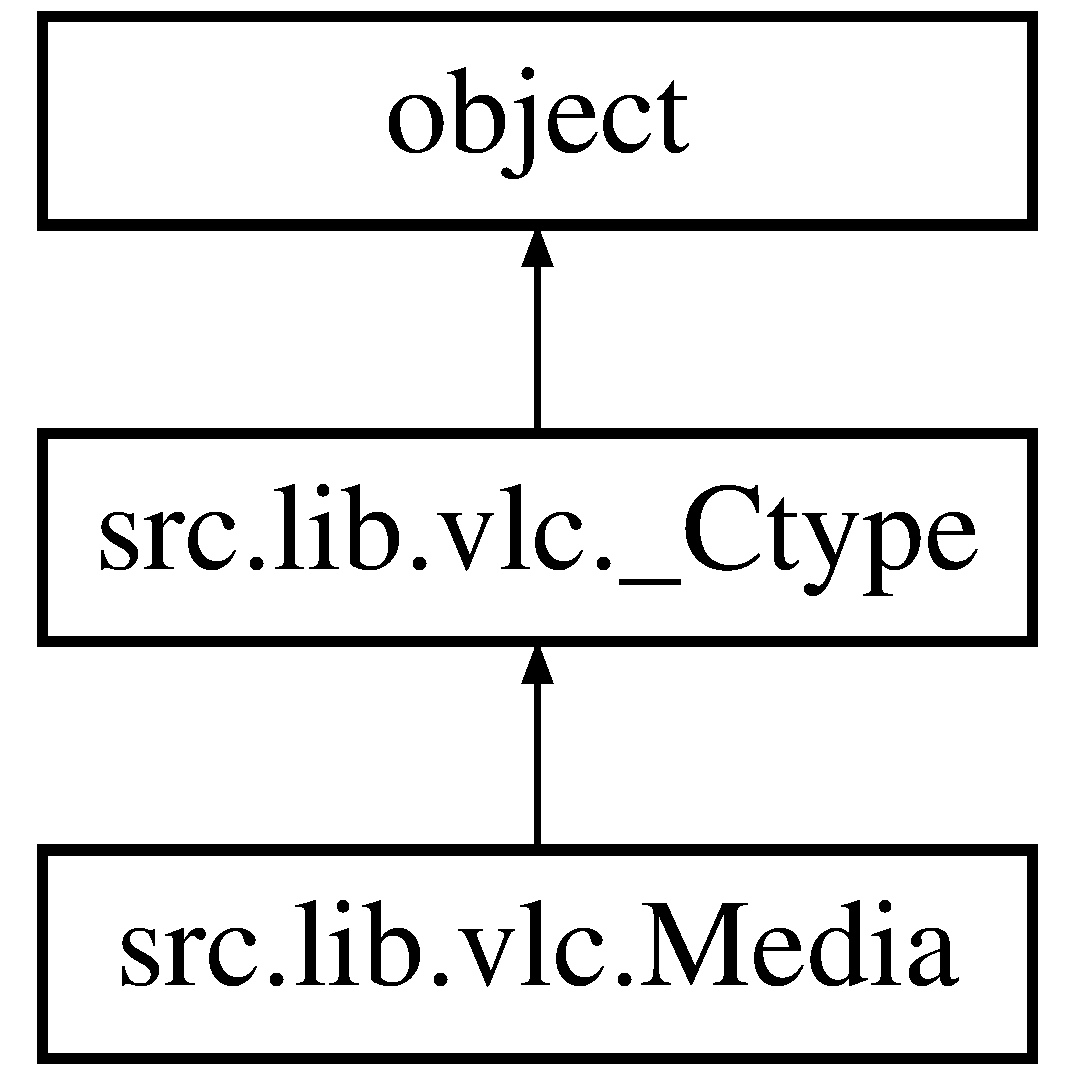
\includegraphics[height=3.000000cm]{classsrc_1_1lib_1_1vlc_1_1Media}
\end{center}
\end{figure}
\subsection*{Public Member Functions}
\begin{DoxyCompactItemize}
\item 
def \hyperlink{classsrc_1_1lib_1_1vlc_1_1Media_a142ae131a221b149de9bc798e9f076f4}{\+\_\+\+\_\+new\+\_\+\+\_\+} (cls, args)
\item 
def \hyperlink{classsrc_1_1lib_1_1vlc_1_1Media_a58142c2e19903edf38de826f6a14d79f}{get\+\_\+instance} (self)
\item 
def \hyperlink{classsrc_1_1lib_1_1vlc_1_1Media_ac3be24ef6e3783406704eb9e6bb8287c}{add\+\_\+options} (self, options)
\item 
def \hyperlink{classsrc_1_1lib_1_1vlc_1_1Media_abad84c4add2b05c53b9fde0a3770c7a7}{add\+\_\+option} (self, ppsz\+\_\+options)
\item 
def \hyperlink{classsrc_1_1lib_1_1vlc_1_1Media_a8af73e42911c4edc74b83a8349b0f08c}{add\+\_\+option\+\_\+flag} (self, ppsz\+\_\+options, i\+\_\+flags)
\item 
def \hyperlink{classsrc_1_1lib_1_1vlc_1_1Media_af418767f78d273f3a6333bc6409acbf0}{retain} (self)
\item 
def \hyperlink{classsrc_1_1lib_1_1vlc_1_1Media_a78f84facb442b8436626de8ccd30dba2}{release} (self)
\item 
def \hyperlink{classsrc_1_1lib_1_1vlc_1_1Media_a8c01cb6f3b79528190988f77fd2b12f8}{get\+\_\+mrl} (self)
\item 
def \hyperlink{classsrc_1_1lib_1_1vlc_1_1Media_ab46200b100bfcf138bc94026b34c78ec}{duplicate} (self)
\item 
def \hyperlink{classsrc_1_1lib_1_1vlc_1_1Media_a4ee1be5ada95e0f32552c7898b458092}{get\+\_\+meta} (self, e\+\_\+meta)
\item 
def \hyperlink{classsrc_1_1lib_1_1vlc_1_1Media_a97554b26343f00f1a35dd6ecc3caf58b}{set\+\_\+meta} (self, e\+\_\+meta, psz\+\_\+value)
\item 
def \hyperlink{classsrc_1_1lib_1_1vlc_1_1Media_aeee361ad7cfab38a3172608a4e475e87}{save\+\_\+meta} (self)
\item 
def \hyperlink{classsrc_1_1lib_1_1vlc_1_1Media_a168ad642702032fee2c3bdf7d2e6f5db}{get\+\_\+state} (self)
\item 
def \hyperlink{classsrc_1_1lib_1_1vlc_1_1Media_add9ecc3f5b46a2bf7392edcadbb7d62e}{get\+\_\+stats} (self, p\+\_\+stats)
\item 
def \hyperlink{classsrc_1_1lib_1_1vlc_1_1Media_aa93f27f97389c5c29780b19b36b16fd0}{event\+\_\+manager} (self)
\item 
def \hyperlink{classsrc_1_1lib_1_1vlc_1_1Media_a8b9ea7e9b8c5d1d49c3f87e496494c0f}{get\+\_\+duration} (self)
\item 
def \hyperlink{classsrc_1_1lib_1_1vlc_1_1Media_a3bf0f5d50d043aef62ebbd9173dc25c5}{parse} (self)
\item 
def \hyperlink{classsrc_1_1lib_1_1vlc_1_1Media_a12d7450b2a71bea1c2b0251fafee6eb3}{parse\+\_\+async} (self)
\item 
def \hyperlink{classsrc_1_1lib_1_1vlc_1_1Media_af04498262d9b6173eb8fa008552f8704}{is\+\_\+parsed} (self)
\item 
def \hyperlink{classsrc_1_1lib_1_1vlc_1_1Media_ac67742341c5217ad70b0be368746c123}{set\+\_\+user\+\_\+data} (self, p\+\_\+new\+\_\+user\+\_\+data)
\item 
def \hyperlink{classsrc_1_1lib_1_1vlc_1_1Media_ade1cf3e752cb5b5428212da0ef571455}{get\+\_\+user\+\_\+data} (self)
\item 
def \hyperlink{classsrc_1_1lib_1_1vlc_1_1Media_a307cc1bbba06fc994594932773c1187e}{get\+\_\+tracks\+\_\+info} (self)
\item 
def \hyperlink{classsrc_1_1lib_1_1vlc_1_1Media_aacfd8f6c83566c722683013860fa064c}{player\+\_\+new\+\_\+from\+\_\+media} (self)
\end{DoxyCompactItemize}
\subsection*{Additional Inherited Members}


\subsection{Detailed Description}
\begin{DoxyVerb}Create a new Media instance.

Usage: Media(MRL, *options)

See vlc.Instance.media_new documentation for details.\end{DoxyVerb}
 

\subsection{Member Function Documentation}
\hypertarget{classsrc_1_1lib_1_1vlc_1_1Media_a142ae131a221b149de9bc798e9f076f4}{}\index{src\+::lib\+::vlc\+::\+Media@{src\+::lib\+::vlc\+::\+Media}!\+\_\+\+\_\+new\+\_\+\+\_\+@{\+\_\+\+\_\+new\+\_\+\+\_\+}}
\index{\+\_\+\+\_\+new\+\_\+\+\_\+@{\+\_\+\+\_\+new\+\_\+\+\_\+}!src\+::lib\+::vlc\+::\+Media@{src\+::lib\+::vlc\+::\+Media}}
\subsubsection[{\+\_\+\+\_\+new\+\_\+\+\_\+}]{\setlength{\rightskip}{0pt plus 5cm}def src.\+lib.\+vlc.\+Media.\+\_\+\+\_\+new\+\_\+\+\_\+ (
\begin{DoxyParamCaption}
\item[{}]{cls, }
\item[{}]{args}
\end{DoxyParamCaption}
)}\label{classsrc_1_1lib_1_1vlc_1_1Media_a142ae131a221b149de9bc798e9f076f4}
\hypertarget{classsrc_1_1lib_1_1vlc_1_1Media_abad84c4add2b05c53b9fde0a3770c7a7}{}\index{src\+::lib\+::vlc\+::\+Media@{src\+::lib\+::vlc\+::\+Media}!add\+\_\+option@{add\+\_\+option}}
\index{add\+\_\+option@{add\+\_\+option}!src\+::lib\+::vlc\+::\+Media@{src\+::lib\+::vlc\+::\+Media}}
\subsubsection[{add\+\_\+option}]{\setlength{\rightskip}{0pt plus 5cm}def src.\+lib.\+vlc.\+Media.\+add\+\_\+option (
\begin{DoxyParamCaption}
\item[{}]{self, }
\item[{}]{ppsz\+\_\+options}
\end{DoxyParamCaption}
)}\label{classsrc_1_1lib_1_1vlc_1_1Media_abad84c4add2b05c53b9fde0a3770c7a7}
\begin{DoxyVerb}Add an option to the media.
This option will be used to determine how the media_player will
read the media. This allows to use VLC's advanced
reading/streaming options on a per-media basis.
The options are detailed in vlc --long-help, for instance "--sout-all".
@param ppsz_options: the options (as a string).
\end{DoxyVerb}
 \hypertarget{classsrc_1_1lib_1_1vlc_1_1Media_a8af73e42911c4edc74b83a8349b0f08c}{}\index{src\+::lib\+::vlc\+::\+Media@{src\+::lib\+::vlc\+::\+Media}!add\+\_\+option\+\_\+flag@{add\+\_\+option\+\_\+flag}}
\index{add\+\_\+option\+\_\+flag@{add\+\_\+option\+\_\+flag}!src\+::lib\+::vlc\+::\+Media@{src\+::lib\+::vlc\+::\+Media}}
\subsubsection[{add\+\_\+option\+\_\+flag}]{\setlength{\rightskip}{0pt plus 5cm}def src.\+lib.\+vlc.\+Media.\+add\+\_\+option\+\_\+flag (
\begin{DoxyParamCaption}
\item[{}]{self, }
\item[{}]{ppsz\+\_\+options, }
\item[{}]{i\+\_\+flags}
\end{DoxyParamCaption}
)}\label{classsrc_1_1lib_1_1vlc_1_1Media_a8af73e42911c4edc74b83a8349b0f08c}
\begin{DoxyVerb}Add an option to the media with configurable flags.
This option will be used to determine how the media_player will
read the media. This allows to use VLC's advanced
reading/streaming options on a per-media basis.
The options are detailed in vlc --long-help, for instance "--sout-all".
@param ppsz_options: the options (as a string).
@param i_flags: the flags for this option.
\end{DoxyVerb}
 \hypertarget{classsrc_1_1lib_1_1vlc_1_1Media_ac3be24ef6e3783406704eb9e6bb8287c}{}\index{src\+::lib\+::vlc\+::\+Media@{src\+::lib\+::vlc\+::\+Media}!add\+\_\+options@{add\+\_\+options}}
\index{add\+\_\+options@{add\+\_\+options}!src\+::lib\+::vlc\+::\+Media@{src\+::lib\+::vlc\+::\+Media}}
\subsubsection[{add\+\_\+options}]{\setlength{\rightskip}{0pt plus 5cm}def src.\+lib.\+vlc.\+Media.\+add\+\_\+options (
\begin{DoxyParamCaption}
\item[{}]{self, }
\item[{}]{options}
\end{DoxyParamCaption}
)}\label{classsrc_1_1lib_1_1vlc_1_1Media_ac3be24ef6e3783406704eb9e6bb8287c}
\begin{DoxyVerb}Add a list of options to the media.

Options must be written without the double-dash, e.g.:

C{m.add_options('sub-filter=marq@test{marquee=Hello}', 'video-filter=invert')}

Alternatively, the options can directly be passed in the Instance.media_new method:

C{m = instance.media_new('foo.avi', 'sub-filter=marq@test{marquee=Hello}', 'video-filter=invert')}

@param options: optional media option=value strings
\end{DoxyVerb}
 \hypertarget{classsrc_1_1lib_1_1vlc_1_1Media_ab46200b100bfcf138bc94026b34c78ec}{}\index{src\+::lib\+::vlc\+::\+Media@{src\+::lib\+::vlc\+::\+Media}!duplicate@{duplicate}}
\index{duplicate@{duplicate}!src\+::lib\+::vlc\+::\+Media@{src\+::lib\+::vlc\+::\+Media}}
\subsubsection[{duplicate}]{\setlength{\rightskip}{0pt plus 5cm}def src.\+lib.\+vlc.\+Media.\+duplicate (
\begin{DoxyParamCaption}
\item[{}]{self}
\end{DoxyParamCaption}
)}\label{classsrc_1_1lib_1_1vlc_1_1Media_ab46200b100bfcf138bc94026b34c78ec}
\begin{DoxyVerb}Duplicate a media descriptor object.
\end{DoxyVerb}
 \hypertarget{classsrc_1_1lib_1_1vlc_1_1Media_aa93f27f97389c5c29780b19b36b16fd0}{}\index{src\+::lib\+::vlc\+::\+Media@{src\+::lib\+::vlc\+::\+Media}!event\+\_\+manager@{event\+\_\+manager}}
\index{event\+\_\+manager@{event\+\_\+manager}!src\+::lib\+::vlc\+::\+Media@{src\+::lib\+::vlc\+::\+Media}}
\subsubsection[{event\+\_\+manager}]{\setlength{\rightskip}{0pt plus 5cm}def src.\+lib.\+vlc.\+Media.\+event\+\_\+manager (
\begin{DoxyParamCaption}
\item[{}]{self}
\end{DoxyParamCaption}
)}\label{classsrc_1_1lib_1_1vlc_1_1Media_aa93f27f97389c5c29780b19b36b16fd0}
\begin{DoxyVerb}Get event manager from media descriptor object.
NOTE: this function doesn't increment reference counting.
@return: event manager object.
\end{DoxyVerb}
 \hypertarget{classsrc_1_1lib_1_1vlc_1_1Media_a8b9ea7e9b8c5d1d49c3f87e496494c0f}{}\index{src\+::lib\+::vlc\+::\+Media@{src\+::lib\+::vlc\+::\+Media}!get\+\_\+duration@{get\+\_\+duration}}
\index{get\+\_\+duration@{get\+\_\+duration}!src\+::lib\+::vlc\+::\+Media@{src\+::lib\+::vlc\+::\+Media}}
\subsubsection[{get\+\_\+duration}]{\setlength{\rightskip}{0pt plus 5cm}def src.\+lib.\+vlc.\+Media.\+get\+\_\+duration (
\begin{DoxyParamCaption}
\item[{}]{self}
\end{DoxyParamCaption}
)}\label{classsrc_1_1lib_1_1vlc_1_1Media_a8b9ea7e9b8c5d1d49c3f87e496494c0f}
\begin{DoxyVerb}Get duration (in ms) of media descriptor object item.
@return: duration of media item or -1 on error.
\end{DoxyVerb}
 \hypertarget{classsrc_1_1lib_1_1vlc_1_1Media_a58142c2e19903edf38de826f6a14d79f}{}\index{src\+::lib\+::vlc\+::\+Media@{src\+::lib\+::vlc\+::\+Media}!get\+\_\+instance@{get\+\_\+instance}}
\index{get\+\_\+instance@{get\+\_\+instance}!src\+::lib\+::vlc\+::\+Media@{src\+::lib\+::vlc\+::\+Media}}
\subsubsection[{get\+\_\+instance}]{\setlength{\rightskip}{0pt plus 5cm}def src.\+lib.\+vlc.\+Media.\+get\+\_\+instance (
\begin{DoxyParamCaption}
\item[{}]{self}
\end{DoxyParamCaption}
)}\label{classsrc_1_1lib_1_1vlc_1_1Media_a58142c2e19903edf38de826f6a14d79f}
\hypertarget{classsrc_1_1lib_1_1vlc_1_1Media_a4ee1be5ada95e0f32552c7898b458092}{}\index{src\+::lib\+::vlc\+::\+Media@{src\+::lib\+::vlc\+::\+Media}!get\+\_\+meta@{get\+\_\+meta}}
\index{get\+\_\+meta@{get\+\_\+meta}!src\+::lib\+::vlc\+::\+Media@{src\+::lib\+::vlc\+::\+Media}}
\subsubsection[{get\+\_\+meta}]{\setlength{\rightskip}{0pt plus 5cm}def src.\+lib.\+vlc.\+Media.\+get\+\_\+meta (
\begin{DoxyParamCaption}
\item[{}]{self, }
\item[{}]{e\+\_\+meta}
\end{DoxyParamCaption}
)}\label{classsrc_1_1lib_1_1vlc_1_1Media_a4ee1be5ada95e0f32552c7898b458092}
\begin{DoxyVerb}Read the meta of the media.
If the media has not yet been parsed this will return NULL.
This methods automatically calls L{parse_async}(), so after calling
it you may receive a libvlc_MediaMetaChanged event. If you prefer a synchronous
version ensure that you call L{parse}() before get_meta().
See L{parse}
See L{parse_async}
See libvlc_MediaMetaChanged.
@param e_meta: the meta to read.
@return: the media's meta.
\end{DoxyVerb}
 \hypertarget{classsrc_1_1lib_1_1vlc_1_1Media_a8c01cb6f3b79528190988f77fd2b12f8}{}\index{src\+::lib\+::vlc\+::\+Media@{src\+::lib\+::vlc\+::\+Media}!get\+\_\+mrl@{get\+\_\+mrl}}
\index{get\+\_\+mrl@{get\+\_\+mrl}!src\+::lib\+::vlc\+::\+Media@{src\+::lib\+::vlc\+::\+Media}}
\subsubsection[{get\+\_\+mrl}]{\setlength{\rightskip}{0pt plus 5cm}def src.\+lib.\+vlc.\+Media.\+get\+\_\+mrl (
\begin{DoxyParamCaption}
\item[{}]{self}
\end{DoxyParamCaption}
)}\label{classsrc_1_1lib_1_1vlc_1_1Media_a8c01cb6f3b79528190988f77fd2b12f8}
\begin{DoxyVerb}Get the media resource locator (mrl) from a media descriptor object.
@return: string with mrl of media descriptor object.
\end{DoxyVerb}
 \hypertarget{classsrc_1_1lib_1_1vlc_1_1Media_a168ad642702032fee2c3bdf7d2e6f5db}{}\index{src\+::lib\+::vlc\+::\+Media@{src\+::lib\+::vlc\+::\+Media}!get\+\_\+state@{get\+\_\+state}}
\index{get\+\_\+state@{get\+\_\+state}!src\+::lib\+::vlc\+::\+Media@{src\+::lib\+::vlc\+::\+Media}}
\subsubsection[{get\+\_\+state}]{\setlength{\rightskip}{0pt plus 5cm}def src.\+lib.\+vlc.\+Media.\+get\+\_\+state (
\begin{DoxyParamCaption}
\item[{}]{self}
\end{DoxyParamCaption}
)}\label{classsrc_1_1lib_1_1vlc_1_1Media_a168ad642702032fee2c3bdf7d2e6f5db}
\begin{DoxyVerb}Get current state of media descriptor object. Possible media states
are defined in libvlc_structures.c ( libvlc_NothingSpecial=0,
libvlc_Opening, libvlc_Buffering, libvlc_Playing, libvlc_Paused,
libvlc_Stopped, libvlc_Ended,
libvlc_Error).
See libvlc_state_t.
@return: state of media descriptor object.
\end{DoxyVerb}
 \hypertarget{classsrc_1_1lib_1_1vlc_1_1Media_add9ecc3f5b46a2bf7392edcadbb7d62e}{}\index{src\+::lib\+::vlc\+::\+Media@{src\+::lib\+::vlc\+::\+Media}!get\+\_\+stats@{get\+\_\+stats}}
\index{get\+\_\+stats@{get\+\_\+stats}!src\+::lib\+::vlc\+::\+Media@{src\+::lib\+::vlc\+::\+Media}}
\subsubsection[{get\+\_\+stats}]{\setlength{\rightskip}{0pt plus 5cm}def src.\+lib.\+vlc.\+Media.\+get\+\_\+stats (
\begin{DoxyParamCaption}
\item[{}]{self, }
\item[{}]{p\+\_\+stats}
\end{DoxyParamCaption}
)}\label{classsrc_1_1lib_1_1vlc_1_1Media_add9ecc3f5b46a2bf7392edcadbb7d62e}
\begin{DoxyVerb}Get the current statistics about the media.
@param p_stats:: structure that contain the statistics about the media (this structure must be allocated by the caller).
@return: true if the statistics are available, false otherwise \libvlc_return_bool.
\end{DoxyVerb}
 \hypertarget{classsrc_1_1lib_1_1vlc_1_1Media_a307cc1bbba06fc994594932773c1187e}{}\index{src\+::lib\+::vlc\+::\+Media@{src\+::lib\+::vlc\+::\+Media}!get\+\_\+tracks\+\_\+info@{get\+\_\+tracks\+\_\+info}}
\index{get\+\_\+tracks\+\_\+info@{get\+\_\+tracks\+\_\+info}!src\+::lib\+::vlc\+::\+Media@{src\+::lib\+::vlc\+::\+Media}}
\subsubsection[{get\+\_\+tracks\+\_\+info}]{\setlength{\rightskip}{0pt plus 5cm}def src.\+lib.\+vlc.\+Media.\+get\+\_\+tracks\+\_\+info (
\begin{DoxyParamCaption}
\item[{}]{self}
\end{DoxyParamCaption}
)}\label{classsrc_1_1lib_1_1vlc_1_1Media_a307cc1bbba06fc994594932773c1187e}
\begin{DoxyVerb}Get media descriptor's elementary streams description
Note, you need to call L{parse}() or play the media at least once
before calling this function.
Not doing this will result in an empty array.
@param tracks: address to store an allocated array of Elementary Streams descriptions (must be freed by the caller).
@return: the number of Elementary Streams.
\end{DoxyVerb}
 \hypertarget{classsrc_1_1lib_1_1vlc_1_1Media_ade1cf3e752cb5b5428212da0ef571455}{}\index{src\+::lib\+::vlc\+::\+Media@{src\+::lib\+::vlc\+::\+Media}!get\+\_\+user\+\_\+data@{get\+\_\+user\+\_\+data}}
\index{get\+\_\+user\+\_\+data@{get\+\_\+user\+\_\+data}!src\+::lib\+::vlc\+::\+Media@{src\+::lib\+::vlc\+::\+Media}}
\subsubsection[{get\+\_\+user\+\_\+data}]{\setlength{\rightskip}{0pt plus 5cm}def src.\+lib.\+vlc.\+Media.\+get\+\_\+user\+\_\+data (
\begin{DoxyParamCaption}
\item[{}]{self}
\end{DoxyParamCaption}
)}\label{classsrc_1_1lib_1_1vlc_1_1Media_ade1cf3e752cb5b5428212da0ef571455}
\begin{DoxyVerb}Get media descriptor's user_data. user_data is specialized data
accessed by the host application, VLC.framework uses it as a pointer to
an native object that references a L{Media} pointer.
\end{DoxyVerb}
 \hypertarget{classsrc_1_1lib_1_1vlc_1_1Media_af04498262d9b6173eb8fa008552f8704}{}\index{src\+::lib\+::vlc\+::\+Media@{src\+::lib\+::vlc\+::\+Media}!is\+\_\+parsed@{is\+\_\+parsed}}
\index{is\+\_\+parsed@{is\+\_\+parsed}!src\+::lib\+::vlc\+::\+Media@{src\+::lib\+::vlc\+::\+Media}}
\subsubsection[{is\+\_\+parsed}]{\setlength{\rightskip}{0pt plus 5cm}def src.\+lib.\+vlc.\+Media.\+is\+\_\+parsed (
\begin{DoxyParamCaption}
\item[{}]{self}
\end{DoxyParamCaption}
)}\label{classsrc_1_1lib_1_1vlc_1_1Media_af04498262d9b6173eb8fa008552f8704}
\begin{DoxyVerb}Get Parsed status for media descriptor object.
See libvlc_MediaParsedChanged.
@return: true if media object has been parsed otherwise it returns false \libvlc_return_bool.
\end{DoxyVerb}
 \hypertarget{classsrc_1_1lib_1_1vlc_1_1Media_a3bf0f5d50d043aef62ebbd9173dc25c5}{}\index{src\+::lib\+::vlc\+::\+Media@{src\+::lib\+::vlc\+::\+Media}!parse@{parse}}
\index{parse@{parse}!src\+::lib\+::vlc\+::\+Media@{src\+::lib\+::vlc\+::\+Media}}
\subsubsection[{parse}]{\setlength{\rightskip}{0pt plus 5cm}def src.\+lib.\+vlc.\+Media.\+parse (
\begin{DoxyParamCaption}
\item[{}]{self}
\end{DoxyParamCaption}
)}\label{classsrc_1_1lib_1_1vlc_1_1Media_a3bf0f5d50d043aef62ebbd9173dc25c5}
\begin{DoxyVerb}Parse a media.
This fetches (local) meta data and tracks information.
The method is synchronous.
See L{parse_async}
See L{get_meta}
See L{get_tracks_info}.
\end{DoxyVerb}
 \hypertarget{classsrc_1_1lib_1_1vlc_1_1Media_a12d7450b2a71bea1c2b0251fafee6eb3}{}\index{src\+::lib\+::vlc\+::\+Media@{src\+::lib\+::vlc\+::\+Media}!parse\+\_\+async@{parse\+\_\+async}}
\index{parse\+\_\+async@{parse\+\_\+async}!src\+::lib\+::vlc\+::\+Media@{src\+::lib\+::vlc\+::\+Media}}
\subsubsection[{parse\+\_\+async}]{\setlength{\rightskip}{0pt plus 5cm}def src.\+lib.\+vlc.\+Media.\+parse\+\_\+async (
\begin{DoxyParamCaption}
\item[{}]{self}
\end{DoxyParamCaption}
)}\label{classsrc_1_1lib_1_1vlc_1_1Media_a12d7450b2a71bea1c2b0251fafee6eb3}
\begin{DoxyVerb}Parse a media.
This fetches (local) meta data and tracks information.
The method is the asynchronous of L{parse}().
To track when this is over you can listen to libvlc_MediaParsedChanged
event. However if the media was already parsed you will not receive this
event.
See L{parse}
See libvlc_MediaParsedChanged
See L{get_meta}
See L{get_tracks_info}.
\end{DoxyVerb}
 \hypertarget{classsrc_1_1lib_1_1vlc_1_1Media_aacfd8f6c83566c722683013860fa064c}{}\index{src\+::lib\+::vlc\+::\+Media@{src\+::lib\+::vlc\+::\+Media}!player\+\_\+new\+\_\+from\+\_\+media@{player\+\_\+new\+\_\+from\+\_\+media}}
\index{player\+\_\+new\+\_\+from\+\_\+media@{player\+\_\+new\+\_\+from\+\_\+media}!src\+::lib\+::vlc\+::\+Media@{src\+::lib\+::vlc\+::\+Media}}
\subsubsection[{player\+\_\+new\+\_\+from\+\_\+media}]{\setlength{\rightskip}{0pt plus 5cm}def src.\+lib.\+vlc.\+Media.\+player\+\_\+new\+\_\+from\+\_\+media (
\begin{DoxyParamCaption}
\item[{}]{self}
\end{DoxyParamCaption}
)}\label{classsrc_1_1lib_1_1vlc_1_1Media_aacfd8f6c83566c722683013860fa064c}
\begin{DoxyVerb}Create a Media Player object from a Media.
@return: a new media player object, or NULL on error.
\end{DoxyVerb}
 \hypertarget{classsrc_1_1lib_1_1vlc_1_1Media_a78f84facb442b8436626de8ccd30dba2}{}\index{src\+::lib\+::vlc\+::\+Media@{src\+::lib\+::vlc\+::\+Media}!release@{release}}
\index{release@{release}!src\+::lib\+::vlc\+::\+Media@{src\+::lib\+::vlc\+::\+Media}}
\subsubsection[{release}]{\setlength{\rightskip}{0pt plus 5cm}def src.\+lib.\+vlc.\+Media.\+release (
\begin{DoxyParamCaption}
\item[{}]{self}
\end{DoxyParamCaption}
)}\label{classsrc_1_1lib_1_1vlc_1_1Media_a78f84facb442b8436626de8ccd30dba2}
\begin{DoxyVerb}Decrement the reference count of a media descriptor object. If the
reference count is 0, then L{release}() will release the
media descriptor object. It will send out an libvlc_MediaFreed event
to all listeners. If the media descriptor object has been released it
should not be used again.
\end{DoxyVerb}
 \hypertarget{classsrc_1_1lib_1_1vlc_1_1Media_af418767f78d273f3a6333bc6409acbf0}{}\index{src\+::lib\+::vlc\+::\+Media@{src\+::lib\+::vlc\+::\+Media}!retain@{retain}}
\index{retain@{retain}!src\+::lib\+::vlc\+::\+Media@{src\+::lib\+::vlc\+::\+Media}}
\subsubsection[{retain}]{\setlength{\rightskip}{0pt plus 5cm}def src.\+lib.\+vlc.\+Media.\+retain (
\begin{DoxyParamCaption}
\item[{}]{self}
\end{DoxyParamCaption}
)}\label{classsrc_1_1lib_1_1vlc_1_1Media_af418767f78d273f3a6333bc6409acbf0}
\begin{DoxyVerb}Retain a reference to a media descriptor object (libvlc_media_t). Use
L{release}() to decrement the reference count of a
media descriptor object.
\end{DoxyVerb}
 \hypertarget{classsrc_1_1lib_1_1vlc_1_1Media_aeee361ad7cfab38a3172608a4e475e87}{}\index{src\+::lib\+::vlc\+::\+Media@{src\+::lib\+::vlc\+::\+Media}!save\+\_\+meta@{save\+\_\+meta}}
\index{save\+\_\+meta@{save\+\_\+meta}!src\+::lib\+::vlc\+::\+Media@{src\+::lib\+::vlc\+::\+Media}}
\subsubsection[{save\+\_\+meta}]{\setlength{\rightskip}{0pt plus 5cm}def src.\+lib.\+vlc.\+Media.\+save\+\_\+meta (
\begin{DoxyParamCaption}
\item[{}]{self}
\end{DoxyParamCaption}
)}\label{classsrc_1_1lib_1_1vlc_1_1Media_aeee361ad7cfab38a3172608a4e475e87}
\begin{DoxyVerb}Save the meta previously set.
@return: true if the write operation was successful.
\end{DoxyVerb}
 \hypertarget{classsrc_1_1lib_1_1vlc_1_1Media_a97554b26343f00f1a35dd6ecc3caf58b}{}\index{src\+::lib\+::vlc\+::\+Media@{src\+::lib\+::vlc\+::\+Media}!set\+\_\+meta@{set\+\_\+meta}}
\index{set\+\_\+meta@{set\+\_\+meta}!src\+::lib\+::vlc\+::\+Media@{src\+::lib\+::vlc\+::\+Media}}
\subsubsection[{set\+\_\+meta}]{\setlength{\rightskip}{0pt plus 5cm}def src.\+lib.\+vlc.\+Media.\+set\+\_\+meta (
\begin{DoxyParamCaption}
\item[{}]{self, }
\item[{}]{e\+\_\+meta, }
\item[{}]{psz\+\_\+value}
\end{DoxyParamCaption}
)}\label{classsrc_1_1lib_1_1vlc_1_1Media_a97554b26343f00f1a35dd6ecc3caf58b}
\begin{DoxyVerb}Set the meta of the media (this function will not save the meta, call
L{save_meta} in order to save the meta).
@param e_meta: the meta to write.
@param psz_value: the media's meta.
\end{DoxyVerb}
 \hypertarget{classsrc_1_1lib_1_1vlc_1_1Media_ac67742341c5217ad70b0be368746c123}{}\index{src\+::lib\+::vlc\+::\+Media@{src\+::lib\+::vlc\+::\+Media}!set\+\_\+user\+\_\+data@{set\+\_\+user\+\_\+data}}
\index{set\+\_\+user\+\_\+data@{set\+\_\+user\+\_\+data}!src\+::lib\+::vlc\+::\+Media@{src\+::lib\+::vlc\+::\+Media}}
\subsubsection[{set\+\_\+user\+\_\+data}]{\setlength{\rightskip}{0pt plus 5cm}def src.\+lib.\+vlc.\+Media.\+set\+\_\+user\+\_\+data (
\begin{DoxyParamCaption}
\item[{}]{self, }
\item[{}]{p\+\_\+new\+\_\+user\+\_\+data}
\end{DoxyParamCaption}
)}\label{classsrc_1_1lib_1_1vlc_1_1Media_ac67742341c5217ad70b0be368746c123}
\begin{DoxyVerb}Sets media descriptor's user_data. user_data is specialized data
accessed by the host application, VLC.framework uses it as a pointer to
an native object that references a L{Media} pointer.
@param p_new_user_data: pointer to user data.
\end{DoxyVerb}
 

The documentation for this class was generated from the following file\+:\begin{DoxyCompactItemize}
\item 
src/lib/\hyperlink{vlc_8py}{vlc.\+py}\end{DoxyCompactItemize}

\hypertarget{classsrc_1_1lib_1_1vlc_1_1MediaDiscoverer}{}\section{src.\+lib.\+vlc.\+Media\+Discoverer Class Reference}
\label{classsrc_1_1lib_1_1vlc_1_1MediaDiscoverer}\index{src.\+lib.\+vlc.\+Media\+Discoverer@{src.\+lib.\+vlc.\+Media\+Discoverer}}
Inheritance diagram for src.\+lib.\+vlc.\+Media\+Discoverer\+:\begin{figure}[H]
\begin{center}
\leavevmode
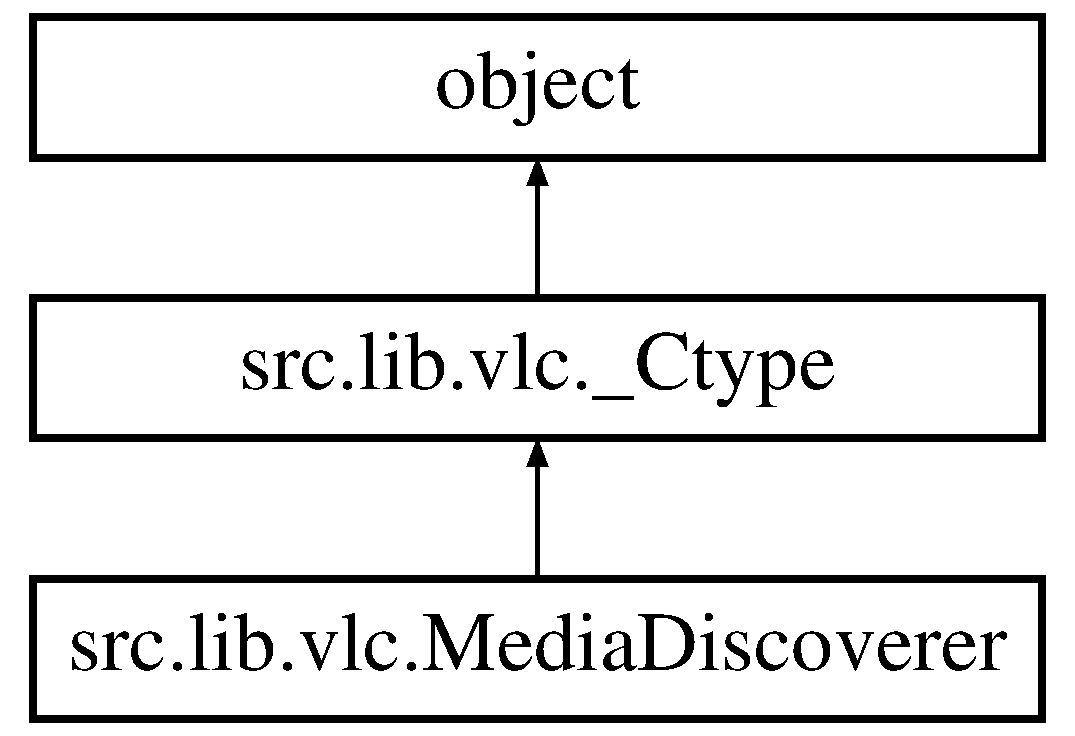
\includegraphics[height=3.000000cm]{classsrc_1_1lib_1_1vlc_1_1MediaDiscoverer}
\end{center}
\end{figure}
\subsection*{Public Member Functions}
\begin{DoxyCompactItemize}
\item 
def \hyperlink{classsrc_1_1lib_1_1vlc_1_1MediaDiscoverer_a7c299935815ecc37c8b6f06712550fb1}{\+\_\+\+\_\+new\+\_\+\+\_\+}
\item 
def \hyperlink{classsrc_1_1lib_1_1vlc_1_1MediaDiscoverer_aae27da52a978a76c1389aa19fa976a9b}{release} (self)
\item 
def \hyperlink{classsrc_1_1lib_1_1vlc_1_1MediaDiscoverer_ad9d0e9d2259970390c1432db14e0b9a5}{localized\+\_\+name} (self)
\item 
def \hyperlink{classsrc_1_1lib_1_1vlc_1_1MediaDiscoverer_ad265055daf05e3b7eb359c7ff0a29bb8}{media\+\_\+list} (self)
\item 
def \hyperlink{classsrc_1_1lib_1_1vlc_1_1MediaDiscoverer_ac9c5181fa862a3ea80fc4d1abdeb0b65}{event\+\_\+manager} (self)
\item 
def \hyperlink{classsrc_1_1lib_1_1vlc_1_1MediaDiscoverer_a353666dc1662f726584044886af40895}{is\+\_\+running} (self)
\end{DoxyCompactItemize}
\subsection*{Additional Inherited Members}


\subsection{Detailed Description}
\begin{DoxyVerb}N/A
\end{DoxyVerb}
 

\subsection{Member Function Documentation}
\hypertarget{classsrc_1_1lib_1_1vlc_1_1MediaDiscoverer_a7c299935815ecc37c8b6f06712550fb1}{}\index{src\+::lib\+::vlc\+::\+Media\+Discoverer@{src\+::lib\+::vlc\+::\+Media\+Discoverer}!\+\_\+\+\_\+new\+\_\+\+\_\+@{\+\_\+\+\_\+new\+\_\+\+\_\+}}
\index{\+\_\+\+\_\+new\+\_\+\+\_\+@{\+\_\+\+\_\+new\+\_\+\+\_\+}!src\+::lib\+::vlc\+::\+Media\+Discoverer@{src\+::lib\+::vlc\+::\+Media\+Discoverer}}
\subsubsection[{\+\_\+\+\_\+new\+\_\+\+\_\+}]{\setlength{\rightskip}{0pt plus 5cm}def src.\+lib.\+vlc.\+Media\+Discoverer.\+\_\+\+\_\+new\+\_\+\+\_\+ (
\begin{DoxyParamCaption}
\item[{}]{cls, }
\item[{}]{ptr = {\ttfamily {\bf \+\_\+internal\+\_\+guard}}}
\end{DoxyParamCaption}
)}\label{classsrc_1_1lib_1_1vlc_1_1MediaDiscoverer_a7c299935815ecc37c8b6f06712550fb1}
\begin{DoxyVerb}(INTERNAL) ctypes wrapper constructor.
\end{DoxyVerb}
 \hypertarget{classsrc_1_1lib_1_1vlc_1_1MediaDiscoverer_ac9c5181fa862a3ea80fc4d1abdeb0b65}{}\index{src\+::lib\+::vlc\+::\+Media\+Discoverer@{src\+::lib\+::vlc\+::\+Media\+Discoverer}!event\+\_\+manager@{event\+\_\+manager}}
\index{event\+\_\+manager@{event\+\_\+manager}!src\+::lib\+::vlc\+::\+Media\+Discoverer@{src\+::lib\+::vlc\+::\+Media\+Discoverer}}
\subsubsection[{event\+\_\+manager}]{\setlength{\rightskip}{0pt plus 5cm}def src.\+lib.\+vlc.\+Media\+Discoverer.\+event\+\_\+manager (
\begin{DoxyParamCaption}
\item[{}]{self}
\end{DoxyParamCaption}
)}\label{classsrc_1_1lib_1_1vlc_1_1MediaDiscoverer_ac9c5181fa862a3ea80fc4d1abdeb0b65}
\begin{DoxyVerb}Get event manager from media service discover object.
@return: event manager object.
\end{DoxyVerb}
 \hypertarget{classsrc_1_1lib_1_1vlc_1_1MediaDiscoverer_a353666dc1662f726584044886af40895}{}\index{src\+::lib\+::vlc\+::\+Media\+Discoverer@{src\+::lib\+::vlc\+::\+Media\+Discoverer}!is\+\_\+running@{is\+\_\+running}}
\index{is\+\_\+running@{is\+\_\+running}!src\+::lib\+::vlc\+::\+Media\+Discoverer@{src\+::lib\+::vlc\+::\+Media\+Discoverer}}
\subsubsection[{is\+\_\+running}]{\setlength{\rightskip}{0pt plus 5cm}def src.\+lib.\+vlc.\+Media\+Discoverer.\+is\+\_\+running (
\begin{DoxyParamCaption}
\item[{}]{self}
\end{DoxyParamCaption}
)}\label{classsrc_1_1lib_1_1vlc_1_1MediaDiscoverer_a353666dc1662f726584044886af40895}
\begin{DoxyVerb}Query if media service discover object is running.
@return: true if running, false if not \libvlc_return_bool.
\end{DoxyVerb}
 \hypertarget{classsrc_1_1lib_1_1vlc_1_1MediaDiscoverer_ad9d0e9d2259970390c1432db14e0b9a5}{}\index{src\+::lib\+::vlc\+::\+Media\+Discoverer@{src\+::lib\+::vlc\+::\+Media\+Discoverer}!localized\+\_\+name@{localized\+\_\+name}}
\index{localized\+\_\+name@{localized\+\_\+name}!src\+::lib\+::vlc\+::\+Media\+Discoverer@{src\+::lib\+::vlc\+::\+Media\+Discoverer}}
\subsubsection[{localized\+\_\+name}]{\setlength{\rightskip}{0pt plus 5cm}def src.\+lib.\+vlc.\+Media\+Discoverer.\+localized\+\_\+name (
\begin{DoxyParamCaption}
\item[{}]{self}
\end{DoxyParamCaption}
)}\label{classsrc_1_1lib_1_1vlc_1_1MediaDiscoverer_ad9d0e9d2259970390c1432db14e0b9a5}
\begin{DoxyVerb}Get media service discover object its localized name.
@return: localized name.
\end{DoxyVerb}
 \hypertarget{classsrc_1_1lib_1_1vlc_1_1MediaDiscoverer_ad265055daf05e3b7eb359c7ff0a29bb8}{}\index{src\+::lib\+::vlc\+::\+Media\+Discoverer@{src\+::lib\+::vlc\+::\+Media\+Discoverer}!media\+\_\+list@{media\+\_\+list}}
\index{media\+\_\+list@{media\+\_\+list}!src\+::lib\+::vlc\+::\+Media\+Discoverer@{src\+::lib\+::vlc\+::\+Media\+Discoverer}}
\subsubsection[{media\+\_\+list}]{\setlength{\rightskip}{0pt plus 5cm}def src.\+lib.\+vlc.\+Media\+Discoverer.\+media\+\_\+list (
\begin{DoxyParamCaption}
\item[{}]{self}
\end{DoxyParamCaption}
)}\label{classsrc_1_1lib_1_1vlc_1_1MediaDiscoverer_ad265055daf05e3b7eb359c7ff0a29bb8}
\begin{DoxyVerb}Get media service discover media list.
@return: list of media items.
\end{DoxyVerb}
 \hypertarget{classsrc_1_1lib_1_1vlc_1_1MediaDiscoverer_aae27da52a978a76c1389aa19fa976a9b}{}\index{src\+::lib\+::vlc\+::\+Media\+Discoverer@{src\+::lib\+::vlc\+::\+Media\+Discoverer}!release@{release}}
\index{release@{release}!src\+::lib\+::vlc\+::\+Media\+Discoverer@{src\+::lib\+::vlc\+::\+Media\+Discoverer}}
\subsubsection[{release}]{\setlength{\rightskip}{0pt plus 5cm}def src.\+lib.\+vlc.\+Media\+Discoverer.\+release (
\begin{DoxyParamCaption}
\item[{}]{self}
\end{DoxyParamCaption}
)}\label{classsrc_1_1lib_1_1vlc_1_1MediaDiscoverer_aae27da52a978a76c1389aa19fa976a9b}
\begin{DoxyVerb}Release media discover object. If the reference count reaches 0, then
the object will be released.
\end{DoxyVerb}
 

The documentation for this class was generated from the following file\+:\begin{DoxyCompactItemize}
\item 
src/lib/\hyperlink{vlc_8py}{vlc.\+py}\end{DoxyCompactItemize}

\hypertarget{classsrc_1_1lib_1_1vlc_1_1MediaEvent}{}\section{src.\+lib.\+vlc.\+Media\+Event Class Reference}
\label{classsrc_1_1lib_1_1vlc_1_1MediaEvent}\index{src.\+lib.\+vlc.\+Media\+Event@{src.\+lib.\+vlc.\+Media\+Event}}
Inheritance diagram for src.\+lib.\+vlc.\+Media\+Event\+:\begin{figure}[H]
\begin{center}
\leavevmode
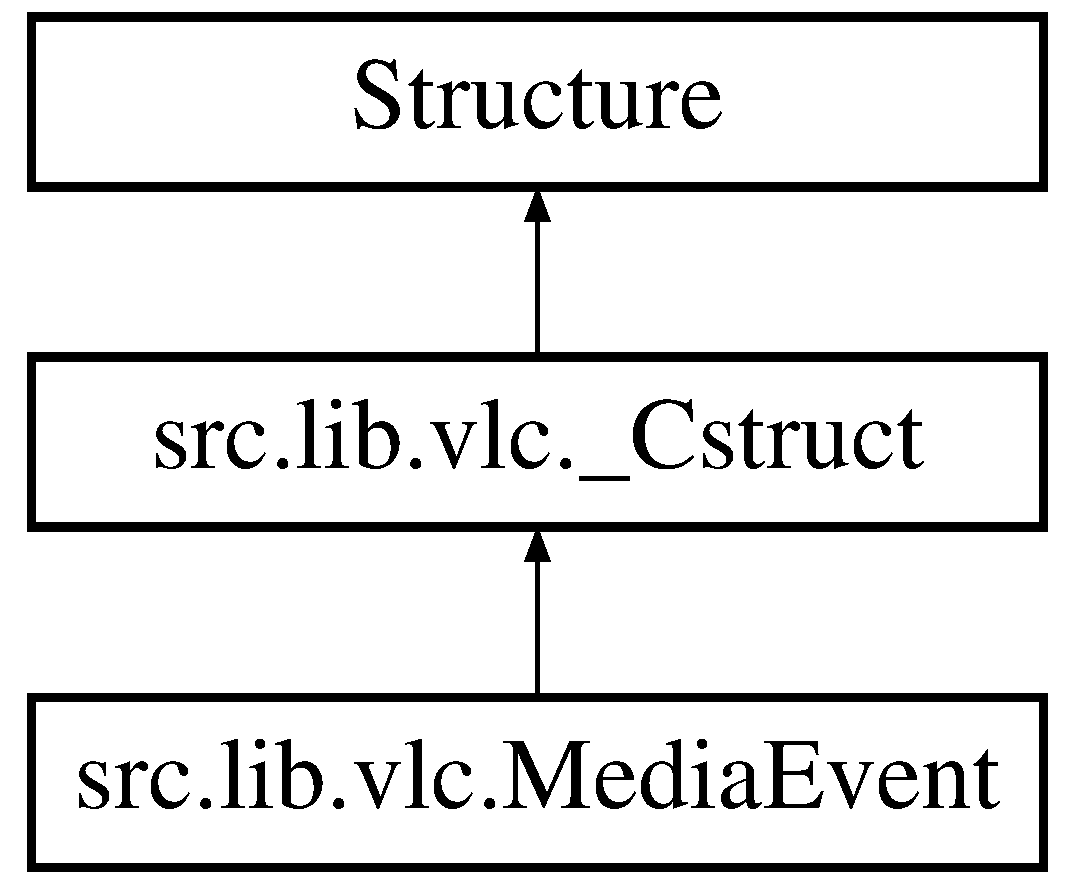
\includegraphics[height=3.000000cm]{classsrc_1_1lib_1_1vlc_1_1MediaEvent}
\end{center}
\end{figure}
\subsection*{Static Private Attributes}
\begin{DoxyCompactItemize}
\item 
list \hyperlink{classsrc_1_1lib_1_1vlc_1_1MediaEvent_a252ea3d8299aec9074ab50a2b86accf3}{\+\_\+fields\+\_\+}
\end{DoxyCompactItemize}
\subsection*{Additional Inherited Members}


\subsection{Member Data Documentation}
\hypertarget{classsrc_1_1lib_1_1vlc_1_1MediaEvent_a252ea3d8299aec9074ab50a2b86accf3}{}\index{src\+::lib\+::vlc\+::\+Media\+Event@{src\+::lib\+::vlc\+::\+Media\+Event}!\+\_\+fields\+\_\+@{\+\_\+fields\+\_\+}}
\index{\+\_\+fields\+\_\+@{\+\_\+fields\+\_\+}!src\+::lib\+::vlc\+::\+Media\+Event@{src\+::lib\+::vlc\+::\+Media\+Event}}
\subsubsection[{\+\_\+fields\+\_\+}]{\setlength{\rightskip}{0pt plus 5cm}list src.\+lib.\+vlc.\+Media\+Event.\+\_\+fields\+\_\+\hspace{0.3cm}{\ttfamily [static]}, {\ttfamily [private]}}\label{classsrc_1_1lib_1_1vlc_1_1MediaEvent_a252ea3d8299aec9074ab50a2b86accf3}
{\bfseries Initial value\+:}
\begin{DoxyCode}
1 = [
2         (\textcolor{stringliteral}{'media\_name'},    ctypes.c\_char\_p),
3         (\textcolor{stringliteral}{'instance\_name'}, ctypes.c\_char\_p),
4     ]
\end{DoxyCode}


The documentation for this class was generated from the following file\+:\begin{DoxyCompactItemize}
\item 
src/lib/\hyperlink{vlc_8py}{vlc.\+py}\end{DoxyCompactItemize}

\hypertarget{classsrc_1_1lib_1_1vlc_1_1MediaLibrary}{}\section{src.\+lib.\+vlc.\+Media\+Library Class Reference}
\label{classsrc_1_1lib_1_1vlc_1_1MediaLibrary}\index{src.\+lib.\+vlc.\+Media\+Library@{src.\+lib.\+vlc.\+Media\+Library}}
Inheritance diagram for src.\+lib.\+vlc.\+Media\+Library\+:\begin{figure}[H]
\begin{center}
\leavevmode
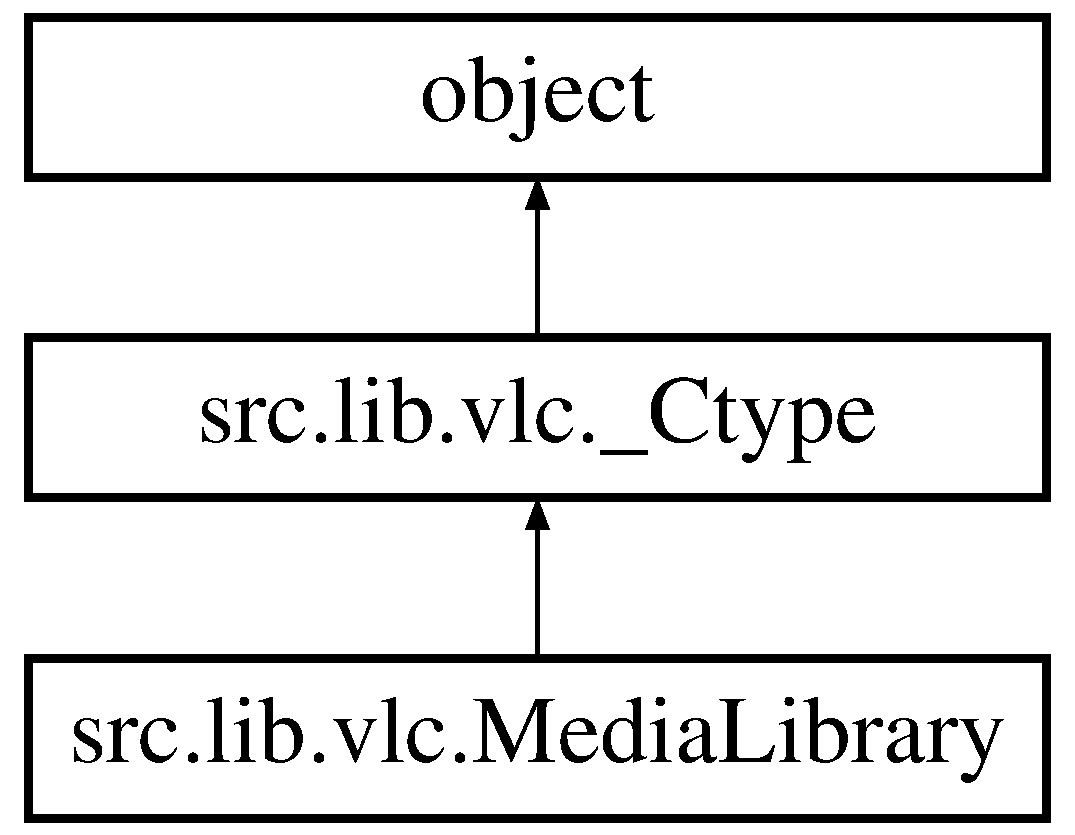
\includegraphics[height=3.000000cm]{classsrc_1_1lib_1_1vlc_1_1MediaLibrary}
\end{center}
\end{figure}
\subsection*{Public Member Functions}
\begin{DoxyCompactItemize}
\item 
def \hyperlink{classsrc_1_1lib_1_1vlc_1_1MediaLibrary_aa659fb06dfc21a3b32fb24b89b6945ce}{\+\_\+\+\_\+new\+\_\+\+\_\+}
\item 
def \hyperlink{classsrc_1_1lib_1_1vlc_1_1MediaLibrary_ac18b86460e74aad8ea0dd2638d4aa192}{release} (self)
\item 
def \hyperlink{classsrc_1_1lib_1_1vlc_1_1MediaLibrary_aeeb6d487de70cefee36b6111a0ee060f}{retain} (self)
\item 
def \hyperlink{classsrc_1_1lib_1_1vlc_1_1MediaLibrary_aaad3a742a689db758b6f09bcb583092c}{load} (self)
\item 
def \hyperlink{classsrc_1_1lib_1_1vlc_1_1MediaLibrary_a69b0be01ac5ab728631b1c7c630862e5}{media\+\_\+list} (self)
\end{DoxyCompactItemize}
\subsection*{Additional Inherited Members}


\subsection{Detailed Description}
\begin{DoxyVerb}N/A
\end{DoxyVerb}
 

\subsection{Member Function Documentation}
\hypertarget{classsrc_1_1lib_1_1vlc_1_1MediaLibrary_aa659fb06dfc21a3b32fb24b89b6945ce}{}\index{src\+::lib\+::vlc\+::\+Media\+Library@{src\+::lib\+::vlc\+::\+Media\+Library}!\+\_\+\+\_\+new\+\_\+\+\_\+@{\+\_\+\+\_\+new\+\_\+\+\_\+}}
\index{\+\_\+\+\_\+new\+\_\+\+\_\+@{\+\_\+\+\_\+new\+\_\+\+\_\+}!src\+::lib\+::vlc\+::\+Media\+Library@{src\+::lib\+::vlc\+::\+Media\+Library}}
\subsubsection[{\+\_\+\+\_\+new\+\_\+\+\_\+}]{\setlength{\rightskip}{0pt plus 5cm}def src.\+lib.\+vlc.\+Media\+Library.\+\_\+\+\_\+new\+\_\+\+\_\+ (
\begin{DoxyParamCaption}
\item[{}]{cls, }
\item[{}]{ptr = {\ttfamily {\bf \+\_\+internal\+\_\+guard}}}
\end{DoxyParamCaption}
)}\label{classsrc_1_1lib_1_1vlc_1_1MediaLibrary_aa659fb06dfc21a3b32fb24b89b6945ce}
\begin{DoxyVerb}(INTERNAL) ctypes wrapper constructor.
\end{DoxyVerb}
 \hypertarget{classsrc_1_1lib_1_1vlc_1_1MediaLibrary_aaad3a742a689db758b6f09bcb583092c}{}\index{src\+::lib\+::vlc\+::\+Media\+Library@{src\+::lib\+::vlc\+::\+Media\+Library}!load@{load}}
\index{load@{load}!src\+::lib\+::vlc\+::\+Media\+Library@{src\+::lib\+::vlc\+::\+Media\+Library}}
\subsubsection[{load}]{\setlength{\rightskip}{0pt plus 5cm}def src.\+lib.\+vlc.\+Media\+Library.\+load (
\begin{DoxyParamCaption}
\item[{}]{self}
\end{DoxyParamCaption}
)}\label{classsrc_1_1lib_1_1vlc_1_1MediaLibrary_aaad3a742a689db758b6f09bcb583092c}
\begin{DoxyVerb}Load media library.
@return: 0 on success, -1 on error.
\end{DoxyVerb}
 \hypertarget{classsrc_1_1lib_1_1vlc_1_1MediaLibrary_a69b0be01ac5ab728631b1c7c630862e5}{}\index{src\+::lib\+::vlc\+::\+Media\+Library@{src\+::lib\+::vlc\+::\+Media\+Library}!media\+\_\+list@{media\+\_\+list}}
\index{media\+\_\+list@{media\+\_\+list}!src\+::lib\+::vlc\+::\+Media\+Library@{src\+::lib\+::vlc\+::\+Media\+Library}}
\subsubsection[{media\+\_\+list}]{\setlength{\rightskip}{0pt plus 5cm}def src.\+lib.\+vlc.\+Media\+Library.\+media\+\_\+list (
\begin{DoxyParamCaption}
\item[{}]{self}
\end{DoxyParamCaption}
)}\label{classsrc_1_1lib_1_1vlc_1_1MediaLibrary_a69b0be01ac5ab728631b1c7c630862e5}
\begin{DoxyVerb}Get media library subitems.
@return: media list subitems.
\end{DoxyVerb}
 \hypertarget{classsrc_1_1lib_1_1vlc_1_1MediaLibrary_ac18b86460e74aad8ea0dd2638d4aa192}{}\index{src\+::lib\+::vlc\+::\+Media\+Library@{src\+::lib\+::vlc\+::\+Media\+Library}!release@{release}}
\index{release@{release}!src\+::lib\+::vlc\+::\+Media\+Library@{src\+::lib\+::vlc\+::\+Media\+Library}}
\subsubsection[{release}]{\setlength{\rightskip}{0pt plus 5cm}def src.\+lib.\+vlc.\+Media\+Library.\+release (
\begin{DoxyParamCaption}
\item[{}]{self}
\end{DoxyParamCaption}
)}\label{classsrc_1_1lib_1_1vlc_1_1MediaLibrary_ac18b86460e74aad8ea0dd2638d4aa192}
\begin{DoxyVerb}Release media library object. This functions decrements the
reference count of the media library object. If it reaches 0,
then the object will be released.
\end{DoxyVerb}
 \hypertarget{classsrc_1_1lib_1_1vlc_1_1MediaLibrary_aeeb6d487de70cefee36b6111a0ee060f}{}\index{src\+::lib\+::vlc\+::\+Media\+Library@{src\+::lib\+::vlc\+::\+Media\+Library}!retain@{retain}}
\index{retain@{retain}!src\+::lib\+::vlc\+::\+Media\+Library@{src\+::lib\+::vlc\+::\+Media\+Library}}
\subsubsection[{retain}]{\setlength{\rightskip}{0pt plus 5cm}def src.\+lib.\+vlc.\+Media\+Library.\+retain (
\begin{DoxyParamCaption}
\item[{}]{self}
\end{DoxyParamCaption}
)}\label{classsrc_1_1lib_1_1vlc_1_1MediaLibrary_aeeb6d487de70cefee36b6111a0ee060f}
\begin{DoxyVerb}Retain a reference to a media library object. This function will
increment the reference counting for this object. Use
L{release}() to decrement the reference count.
\end{DoxyVerb}
 

The documentation for this class was generated from the following file\+:\begin{DoxyCompactItemize}
\item 
src/lib/\hyperlink{vlc_8py}{vlc.\+py}\end{DoxyCompactItemize}

\hypertarget{classsrc_1_1lib_1_1vlc_1_1MediaList}{}\section{src.\+lib.\+vlc.\+Media\+List Class Reference}
\label{classsrc_1_1lib_1_1vlc_1_1MediaList}\index{src.\+lib.\+vlc.\+Media\+List@{src.\+lib.\+vlc.\+Media\+List}}
Inheritance diagram for src.\+lib.\+vlc.\+Media\+List\+:\begin{figure}[H]
\begin{center}
\leavevmode
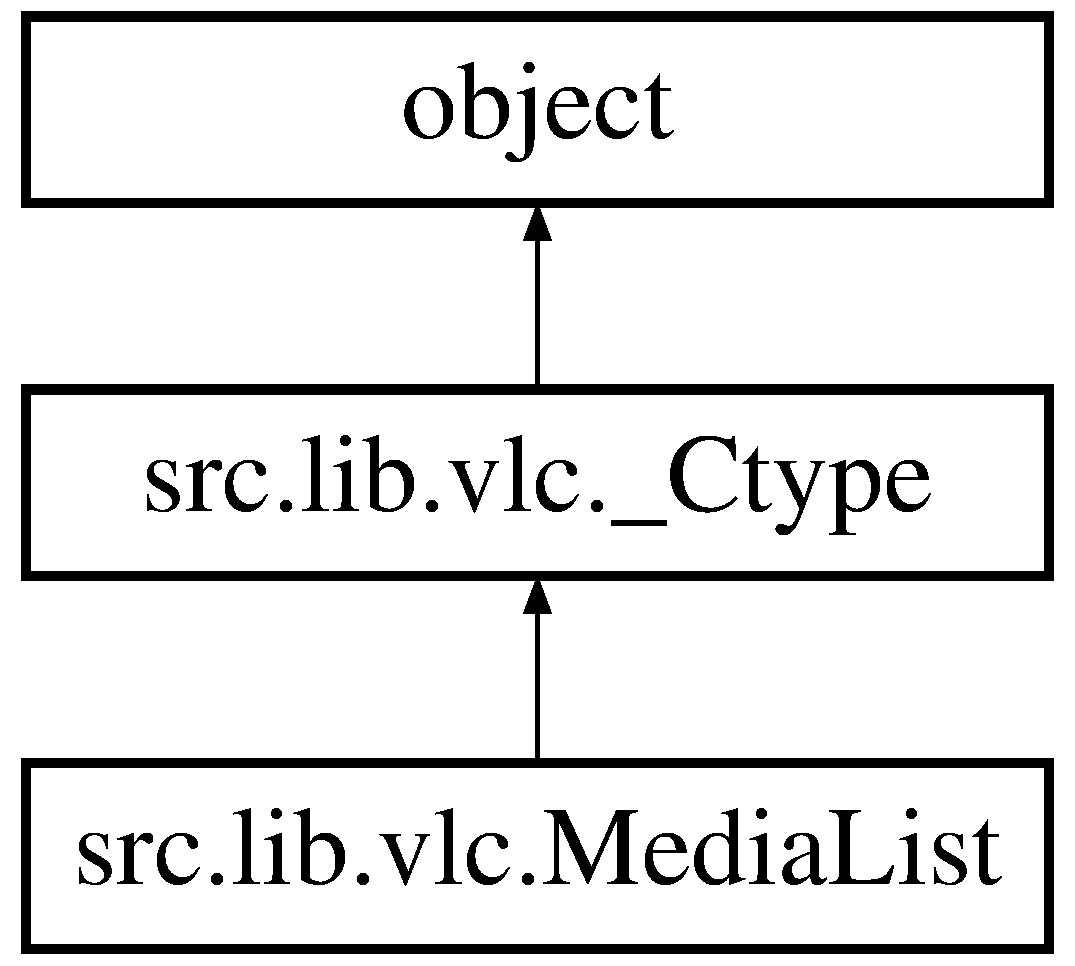
\includegraphics[height=3.000000cm]{classsrc_1_1lib_1_1vlc_1_1MediaList}
\end{center}
\end{figure}
\subsection*{Public Member Functions}
\begin{DoxyCompactItemize}
\item 
def \hyperlink{classsrc_1_1lib_1_1vlc_1_1MediaList_add545be3c6d1e7b59338979fd2ca7d41}{\+\_\+\+\_\+new\+\_\+\+\_\+} (cls, args)
\item 
def \hyperlink{classsrc_1_1lib_1_1vlc_1_1MediaList_ace46e3907c3dfcfbf7e4de8f87cccd7b}{get\+\_\+instance} (self)
\item 
def \hyperlink{classsrc_1_1lib_1_1vlc_1_1MediaList_a4abfc4b299b9ded65d0e01414b29ba12}{add\+\_\+media} (self, mrl)
\item 
def \hyperlink{classsrc_1_1lib_1_1vlc_1_1MediaList_a650b16ef72f2433f0f6c5efee4f15150}{release} (self)
\item 
def \hyperlink{classsrc_1_1lib_1_1vlc_1_1MediaList_a2ff79029718c19f1a13550d8d5214b42}{retain} (self)
\item 
def \hyperlink{classsrc_1_1lib_1_1vlc_1_1MediaList_a90164edbf5deee0b20618df376a0bdbc}{set\+\_\+media} (self, p\+\_\+md)
\item 
def \hyperlink{classsrc_1_1lib_1_1vlc_1_1MediaList_a397d000080e64e0e2325d0b5d9cafac6}{media} (self)
\item 
def \hyperlink{classsrc_1_1lib_1_1vlc_1_1MediaList_ab1d2aecb1245171a160e2cb232bcba09}{insert\+\_\+media} (self, p\+\_\+md, i\+\_\+pos)
\item 
def \hyperlink{classsrc_1_1lib_1_1vlc_1_1MediaList_a713acf30b7bc9738b2c579c3b098e49a}{remove\+\_\+index} (self, i\+\_\+pos)
\item 
def \hyperlink{classsrc_1_1lib_1_1vlc_1_1MediaList_a042a0c4f8a82ae1d3ada30554326fd67}{count} (self)
\item 
def \hyperlink{classsrc_1_1lib_1_1vlc_1_1MediaList_af951143b03143deefde7d1adbe034072}{\+\_\+\+\_\+len\+\_\+\+\_\+} (self)
\item 
def \hyperlink{classsrc_1_1lib_1_1vlc_1_1MediaList_a26e54d4ff1064b281d8f84a5f38b6abc}{item\+\_\+at\+\_\+index} (self, i\+\_\+pos)
\item 
def \hyperlink{classsrc_1_1lib_1_1vlc_1_1MediaList_a69fee887eb9bd11182a2af912335cf19}{\+\_\+\+\_\+getitem\+\_\+\+\_\+} (self, i)
\item 
def \hyperlink{classsrc_1_1lib_1_1vlc_1_1MediaList_a78b5cde7e977455c19ab28e13b4ad7d2}{\+\_\+\+\_\+iter\+\_\+\+\_\+} (self)
\item 
def \hyperlink{classsrc_1_1lib_1_1vlc_1_1MediaList_a36f5b7d100c4033c2a1a15f8f8b8dee3}{index\+\_\+of\+\_\+item} (self, p\+\_\+md)
\item 
def \hyperlink{classsrc_1_1lib_1_1vlc_1_1MediaList_a62d381ecf67d0fd330d570550f835e72}{is\+\_\+readonly} (self)
\item 
def \hyperlink{classsrc_1_1lib_1_1vlc_1_1MediaList_aa1cf61a308cb3545edb336c0d2519df4}{lock} (self)
\item 
def \hyperlink{classsrc_1_1lib_1_1vlc_1_1MediaList_a74b28df20f66095de94201d0a396c36e}{unlock} (self)
\item 
def \hyperlink{classsrc_1_1lib_1_1vlc_1_1MediaList_aa4cfb33fcdcd755c9e17610b72c66948}{event\+\_\+manager} (self)
\end{DoxyCompactItemize}
\subsection*{Additional Inherited Members}


\subsection{Detailed Description}
\begin{DoxyVerb}Create a new MediaList instance.

Usage: MediaList(list_of_MRLs)

See vlc.Instance.media_list_new documentation for details.\end{DoxyVerb}
 

\subsection{Member Function Documentation}
\hypertarget{classsrc_1_1lib_1_1vlc_1_1MediaList_a69fee887eb9bd11182a2af912335cf19}{}\index{src\+::lib\+::vlc\+::\+Media\+List@{src\+::lib\+::vlc\+::\+Media\+List}!\+\_\+\+\_\+getitem\+\_\+\+\_\+@{\+\_\+\+\_\+getitem\+\_\+\+\_\+}}
\index{\+\_\+\+\_\+getitem\+\_\+\+\_\+@{\+\_\+\+\_\+getitem\+\_\+\+\_\+}!src\+::lib\+::vlc\+::\+Media\+List@{src\+::lib\+::vlc\+::\+Media\+List}}
\subsubsection[{\+\_\+\+\_\+getitem\+\_\+\+\_\+}]{\setlength{\rightskip}{0pt plus 5cm}def src.\+lib.\+vlc.\+Media\+List.\+\_\+\+\_\+getitem\+\_\+\+\_\+ (
\begin{DoxyParamCaption}
\item[{}]{self, }
\item[{}]{i}
\end{DoxyParamCaption}
)}\label{classsrc_1_1lib_1_1vlc_1_1MediaList_a69fee887eb9bd11182a2af912335cf19}
\hypertarget{classsrc_1_1lib_1_1vlc_1_1MediaList_a78b5cde7e977455c19ab28e13b4ad7d2}{}\index{src\+::lib\+::vlc\+::\+Media\+List@{src\+::lib\+::vlc\+::\+Media\+List}!\+\_\+\+\_\+iter\+\_\+\+\_\+@{\+\_\+\+\_\+iter\+\_\+\+\_\+}}
\index{\+\_\+\+\_\+iter\+\_\+\+\_\+@{\+\_\+\+\_\+iter\+\_\+\+\_\+}!src\+::lib\+::vlc\+::\+Media\+List@{src\+::lib\+::vlc\+::\+Media\+List}}
\subsubsection[{\+\_\+\+\_\+iter\+\_\+\+\_\+}]{\setlength{\rightskip}{0pt plus 5cm}def src.\+lib.\+vlc.\+Media\+List.\+\_\+\+\_\+iter\+\_\+\+\_\+ (
\begin{DoxyParamCaption}
\item[{}]{self}
\end{DoxyParamCaption}
)}\label{classsrc_1_1lib_1_1vlc_1_1MediaList_a78b5cde7e977455c19ab28e13b4ad7d2}
\hypertarget{classsrc_1_1lib_1_1vlc_1_1MediaList_af951143b03143deefde7d1adbe034072}{}\index{src\+::lib\+::vlc\+::\+Media\+List@{src\+::lib\+::vlc\+::\+Media\+List}!\+\_\+\+\_\+len\+\_\+\+\_\+@{\+\_\+\+\_\+len\+\_\+\+\_\+}}
\index{\+\_\+\+\_\+len\+\_\+\+\_\+@{\+\_\+\+\_\+len\+\_\+\+\_\+}!src\+::lib\+::vlc\+::\+Media\+List@{src\+::lib\+::vlc\+::\+Media\+List}}
\subsubsection[{\+\_\+\+\_\+len\+\_\+\+\_\+}]{\setlength{\rightskip}{0pt plus 5cm}def src.\+lib.\+vlc.\+Media\+List.\+\_\+\+\_\+len\+\_\+\+\_\+ (
\begin{DoxyParamCaption}
\item[{}]{self}
\end{DoxyParamCaption}
)}\label{classsrc_1_1lib_1_1vlc_1_1MediaList_af951143b03143deefde7d1adbe034072}
\hypertarget{classsrc_1_1lib_1_1vlc_1_1MediaList_add545be3c6d1e7b59338979fd2ca7d41}{}\index{src\+::lib\+::vlc\+::\+Media\+List@{src\+::lib\+::vlc\+::\+Media\+List}!\+\_\+\+\_\+new\+\_\+\+\_\+@{\+\_\+\+\_\+new\+\_\+\+\_\+}}
\index{\+\_\+\+\_\+new\+\_\+\+\_\+@{\+\_\+\+\_\+new\+\_\+\+\_\+}!src\+::lib\+::vlc\+::\+Media\+List@{src\+::lib\+::vlc\+::\+Media\+List}}
\subsubsection[{\+\_\+\+\_\+new\+\_\+\+\_\+}]{\setlength{\rightskip}{0pt plus 5cm}def src.\+lib.\+vlc.\+Media\+List.\+\_\+\+\_\+new\+\_\+\+\_\+ (
\begin{DoxyParamCaption}
\item[{}]{cls, }
\item[{}]{args}
\end{DoxyParamCaption}
)}\label{classsrc_1_1lib_1_1vlc_1_1MediaList_add545be3c6d1e7b59338979fd2ca7d41}
\hypertarget{classsrc_1_1lib_1_1vlc_1_1MediaList_a4abfc4b299b9ded65d0e01414b29ba12}{}\index{src\+::lib\+::vlc\+::\+Media\+List@{src\+::lib\+::vlc\+::\+Media\+List}!add\+\_\+media@{add\+\_\+media}}
\index{add\+\_\+media@{add\+\_\+media}!src\+::lib\+::vlc\+::\+Media\+List@{src\+::lib\+::vlc\+::\+Media\+List}}
\subsubsection[{add\+\_\+media}]{\setlength{\rightskip}{0pt plus 5cm}def src.\+lib.\+vlc.\+Media\+List.\+add\+\_\+media (
\begin{DoxyParamCaption}
\item[{}]{self, }
\item[{}]{mrl}
\end{DoxyParamCaption}
)}\label{classsrc_1_1lib_1_1vlc_1_1MediaList_a4abfc4b299b9ded65d0e01414b29ba12}
\begin{DoxyVerb}Add media instance to media list.

The L{lock} should be held upon entering this function.
@param p_md: a media instance or a MRL.
@return: 0 on success, -1 if the media list is read-only.
\end{DoxyVerb}
 \hypertarget{classsrc_1_1lib_1_1vlc_1_1MediaList_a042a0c4f8a82ae1d3ada30554326fd67}{}\index{src\+::lib\+::vlc\+::\+Media\+List@{src\+::lib\+::vlc\+::\+Media\+List}!count@{count}}
\index{count@{count}!src\+::lib\+::vlc\+::\+Media\+List@{src\+::lib\+::vlc\+::\+Media\+List}}
\subsubsection[{count}]{\setlength{\rightskip}{0pt plus 5cm}def src.\+lib.\+vlc.\+Media\+List.\+count (
\begin{DoxyParamCaption}
\item[{}]{self}
\end{DoxyParamCaption}
)}\label{classsrc_1_1lib_1_1vlc_1_1MediaList_a042a0c4f8a82ae1d3ada30554326fd67}
\begin{DoxyVerb}Get count on media list items
The L{lock} should be held upon entering this function.
@return: number of items in media list.
\end{DoxyVerb}
 \hypertarget{classsrc_1_1lib_1_1vlc_1_1MediaList_aa4cfb33fcdcd755c9e17610b72c66948}{}\index{src\+::lib\+::vlc\+::\+Media\+List@{src\+::lib\+::vlc\+::\+Media\+List}!event\+\_\+manager@{event\+\_\+manager}}
\index{event\+\_\+manager@{event\+\_\+manager}!src\+::lib\+::vlc\+::\+Media\+List@{src\+::lib\+::vlc\+::\+Media\+List}}
\subsubsection[{event\+\_\+manager}]{\setlength{\rightskip}{0pt plus 5cm}def src.\+lib.\+vlc.\+Media\+List.\+event\+\_\+manager (
\begin{DoxyParamCaption}
\item[{}]{self}
\end{DoxyParamCaption}
)}\label{classsrc_1_1lib_1_1vlc_1_1MediaList_aa4cfb33fcdcd755c9e17610b72c66948}
\begin{DoxyVerb}Get libvlc_event_manager from this media list instance.
The p_event_manager is immutable, so you don't have to hold the lock.
@return: libvlc_event_manager.
\end{DoxyVerb}
 \hypertarget{classsrc_1_1lib_1_1vlc_1_1MediaList_ace46e3907c3dfcfbf7e4de8f87cccd7b}{}\index{src\+::lib\+::vlc\+::\+Media\+List@{src\+::lib\+::vlc\+::\+Media\+List}!get\+\_\+instance@{get\+\_\+instance}}
\index{get\+\_\+instance@{get\+\_\+instance}!src\+::lib\+::vlc\+::\+Media\+List@{src\+::lib\+::vlc\+::\+Media\+List}}
\subsubsection[{get\+\_\+instance}]{\setlength{\rightskip}{0pt plus 5cm}def src.\+lib.\+vlc.\+Media\+List.\+get\+\_\+instance (
\begin{DoxyParamCaption}
\item[{}]{self}
\end{DoxyParamCaption}
)}\label{classsrc_1_1lib_1_1vlc_1_1MediaList_ace46e3907c3dfcfbf7e4de8f87cccd7b}
\hypertarget{classsrc_1_1lib_1_1vlc_1_1MediaList_a36f5b7d100c4033c2a1a15f8f8b8dee3}{}\index{src\+::lib\+::vlc\+::\+Media\+List@{src\+::lib\+::vlc\+::\+Media\+List}!index\+\_\+of\+\_\+item@{index\+\_\+of\+\_\+item}}
\index{index\+\_\+of\+\_\+item@{index\+\_\+of\+\_\+item}!src\+::lib\+::vlc\+::\+Media\+List@{src\+::lib\+::vlc\+::\+Media\+List}}
\subsubsection[{index\+\_\+of\+\_\+item}]{\setlength{\rightskip}{0pt plus 5cm}def src.\+lib.\+vlc.\+Media\+List.\+index\+\_\+of\+\_\+item (
\begin{DoxyParamCaption}
\item[{}]{self, }
\item[{}]{p\+\_\+md}
\end{DoxyParamCaption}
)}\label{classsrc_1_1lib_1_1vlc_1_1MediaList_a36f5b7d100c4033c2a1a15f8f8b8dee3}
\begin{DoxyVerb}Find index position of List media instance in media list.
Warning: the function will return the first matched position.
The L{lock} should be held upon entering this function.
@param p_md: media instance.
@return: position of media instance or -1 if media not found.
\end{DoxyVerb}
 \hypertarget{classsrc_1_1lib_1_1vlc_1_1MediaList_ab1d2aecb1245171a160e2cb232bcba09}{}\index{src\+::lib\+::vlc\+::\+Media\+List@{src\+::lib\+::vlc\+::\+Media\+List}!insert\+\_\+media@{insert\+\_\+media}}
\index{insert\+\_\+media@{insert\+\_\+media}!src\+::lib\+::vlc\+::\+Media\+List@{src\+::lib\+::vlc\+::\+Media\+List}}
\subsubsection[{insert\+\_\+media}]{\setlength{\rightskip}{0pt plus 5cm}def src.\+lib.\+vlc.\+Media\+List.\+insert\+\_\+media (
\begin{DoxyParamCaption}
\item[{}]{self, }
\item[{}]{p\+\_\+md, }
\item[{}]{i\+\_\+pos}
\end{DoxyParamCaption}
)}\label{classsrc_1_1lib_1_1vlc_1_1MediaList_ab1d2aecb1245171a160e2cb232bcba09}
\begin{DoxyVerb}Insert media instance in media list on a position
The L{lock} should be held upon entering this function.
@param p_md: a media instance.
@param i_pos: position in array where to insert.
@return: 0 on success, -1 if the media list is read-only.
\end{DoxyVerb}
 \hypertarget{classsrc_1_1lib_1_1vlc_1_1MediaList_a62d381ecf67d0fd330d570550f835e72}{}\index{src\+::lib\+::vlc\+::\+Media\+List@{src\+::lib\+::vlc\+::\+Media\+List}!is\+\_\+readonly@{is\+\_\+readonly}}
\index{is\+\_\+readonly@{is\+\_\+readonly}!src\+::lib\+::vlc\+::\+Media\+List@{src\+::lib\+::vlc\+::\+Media\+List}}
\subsubsection[{is\+\_\+readonly}]{\setlength{\rightskip}{0pt plus 5cm}def src.\+lib.\+vlc.\+Media\+List.\+is\+\_\+readonly (
\begin{DoxyParamCaption}
\item[{}]{self}
\end{DoxyParamCaption}
)}\label{classsrc_1_1lib_1_1vlc_1_1MediaList_a62d381ecf67d0fd330d570550f835e72}
\begin{DoxyVerb}This indicates if this media list is read-only from a user point of view.
@return: 1 on readonly, 0 on readwrite \libvlc_return_bool.
\end{DoxyVerb}
 \hypertarget{classsrc_1_1lib_1_1vlc_1_1MediaList_a26e54d4ff1064b281d8f84a5f38b6abc}{}\index{src\+::lib\+::vlc\+::\+Media\+List@{src\+::lib\+::vlc\+::\+Media\+List}!item\+\_\+at\+\_\+index@{item\+\_\+at\+\_\+index}}
\index{item\+\_\+at\+\_\+index@{item\+\_\+at\+\_\+index}!src\+::lib\+::vlc\+::\+Media\+List@{src\+::lib\+::vlc\+::\+Media\+List}}
\subsubsection[{item\+\_\+at\+\_\+index}]{\setlength{\rightskip}{0pt plus 5cm}def src.\+lib.\+vlc.\+Media\+List.\+item\+\_\+at\+\_\+index (
\begin{DoxyParamCaption}
\item[{}]{self, }
\item[{}]{i\+\_\+pos}
\end{DoxyParamCaption}
)}\label{classsrc_1_1lib_1_1vlc_1_1MediaList_a26e54d4ff1064b281d8f84a5f38b6abc}
\begin{DoxyVerb}List media instance in media list at a position
The L{lock} should be held upon entering this function.
@param i_pos: position in array where to insert.
@return: media instance at position i_pos, or NULL if not found. In case of success, L{media_retain}() is called to increase the refcount on the media.
\end{DoxyVerb}
 \hypertarget{classsrc_1_1lib_1_1vlc_1_1MediaList_aa1cf61a308cb3545edb336c0d2519df4}{}\index{src\+::lib\+::vlc\+::\+Media\+List@{src\+::lib\+::vlc\+::\+Media\+List}!lock@{lock}}
\index{lock@{lock}!src\+::lib\+::vlc\+::\+Media\+List@{src\+::lib\+::vlc\+::\+Media\+List}}
\subsubsection[{lock}]{\setlength{\rightskip}{0pt plus 5cm}def src.\+lib.\+vlc.\+Media\+List.\+lock (
\begin{DoxyParamCaption}
\item[{}]{self}
\end{DoxyParamCaption}
)}\label{classsrc_1_1lib_1_1vlc_1_1MediaList_aa1cf61a308cb3545edb336c0d2519df4}
\begin{DoxyVerb}Get lock on media list items.
\end{DoxyVerb}
 \hypertarget{classsrc_1_1lib_1_1vlc_1_1MediaList_a397d000080e64e0e2325d0b5d9cafac6}{}\index{src\+::lib\+::vlc\+::\+Media\+List@{src\+::lib\+::vlc\+::\+Media\+List}!media@{media}}
\index{media@{media}!src\+::lib\+::vlc\+::\+Media\+List@{src\+::lib\+::vlc\+::\+Media\+List}}
\subsubsection[{media}]{\setlength{\rightskip}{0pt plus 5cm}def src.\+lib.\+vlc.\+Media\+List.\+media (
\begin{DoxyParamCaption}
\item[{}]{self}
\end{DoxyParamCaption}
)}\label{classsrc_1_1lib_1_1vlc_1_1MediaList_a397d000080e64e0e2325d0b5d9cafac6}
\begin{DoxyVerb}Get media instance from this media list instance. This action will increase
the refcount on the media instance.
The L{lock} should NOT be held upon entering this function.
@return: media instance.
\end{DoxyVerb}
 \hypertarget{classsrc_1_1lib_1_1vlc_1_1MediaList_a650b16ef72f2433f0f6c5efee4f15150}{}\index{src\+::lib\+::vlc\+::\+Media\+List@{src\+::lib\+::vlc\+::\+Media\+List}!release@{release}}
\index{release@{release}!src\+::lib\+::vlc\+::\+Media\+List@{src\+::lib\+::vlc\+::\+Media\+List}}
\subsubsection[{release}]{\setlength{\rightskip}{0pt plus 5cm}def src.\+lib.\+vlc.\+Media\+List.\+release (
\begin{DoxyParamCaption}
\item[{}]{self}
\end{DoxyParamCaption}
)}\label{classsrc_1_1lib_1_1vlc_1_1MediaList_a650b16ef72f2433f0f6c5efee4f15150}
\begin{DoxyVerb}Release media list created with L{new}().
\end{DoxyVerb}
 \hypertarget{classsrc_1_1lib_1_1vlc_1_1MediaList_a713acf30b7bc9738b2c579c3b098e49a}{}\index{src\+::lib\+::vlc\+::\+Media\+List@{src\+::lib\+::vlc\+::\+Media\+List}!remove\+\_\+index@{remove\+\_\+index}}
\index{remove\+\_\+index@{remove\+\_\+index}!src\+::lib\+::vlc\+::\+Media\+List@{src\+::lib\+::vlc\+::\+Media\+List}}
\subsubsection[{remove\+\_\+index}]{\setlength{\rightskip}{0pt plus 5cm}def src.\+lib.\+vlc.\+Media\+List.\+remove\+\_\+index (
\begin{DoxyParamCaption}
\item[{}]{self, }
\item[{}]{i\+\_\+pos}
\end{DoxyParamCaption}
)}\label{classsrc_1_1lib_1_1vlc_1_1MediaList_a713acf30b7bc9738b2c579c3b098e49a}
\begin{DoxyVerb}Remove media instance from media list on a position
The L{lock} should be held upon entering this function.
@param i_pos: position in array where to insert.
@return: 0 on success, -1 if the list is read-only or the item was not found.
\end{DoxyVerb}
 \hypertarget{classsrc_1_1lib_1_1vlc_1_1MediaList_a2ff79029718c19f1a13550d8d5214b42}{}\index{src\+::lib\+::vlc\+::\+Media\+List@{src\+::lib\+::vlc\+::\+Media\+List}!retain@{retain}}
\index{retain@{retain}!src\+::lib\+::vlc\+::\+Media\+List@{src\+::lib\+::vlc\+::\+Media\+List}}
\subsubsection[{retain}]{\setlength{\rightskip}{0pt plus 5cm}def src.\+lib.\+vlc.\+Media\+List.\+retain (
\begin{DoxyParamCaption}
\item[{}]{self}
\end{DoxyParamCaption}
)}\label{classsrc_1_1lib_1_1vlc_1_1MediaList_a2ff79029718c19f1a13550d8d5214b42}
\begin{DoxyVerb}Retain reference to a media list.
\end{DoxyVerb}
 \hypertarget{classsrc_1_1lib_1_1vlc_1_1MediaList_a90164edbf5deee0b20618df376a0bdbc}{}\index{src\+::lib\+::vlc\+::\+Media\+List@{src\+::lib\+::vlc\+::\+Media\+List}!set\+\_\+media@{set\+\_\+media}}
\index{set\+\_\+media@{set\+\_\+media}!src\+::lib\+::vlc\+::\+Media\+List@{src\+::lib\+::vlc\+::\+Media\+List}}
\subsubsection[{set\+\_\+media}]{\setlength{\rightskip}{0pt plus 5cm}def src.\+lib.\+vlc.\+Media\+List.\+set\+\_\+media (
\begin{DoxyParamCaption}
\item[{}]{self, }
\item[{}]{p\+\_\+md}
\end{DoxyParamCaption}
)}\label{classsrc_1_1lib_1_1vlc_1_1MediaList_a90164edbf5deee0b20618df376a0bdbc}
\begin{DoxyVerb}Associate media instance with this media list instance.
If another media instance was present it will be released.
The L{lock} should NOT be held upon entering this function.
@param p_md: media instance to add.
\end{DoxyVerb}
 \hypertarget{classsrc_1_1lib_1_1vlc_1_1MediaList_a74b28df20f66095de94201d0a396c36e}{}\index{src\+::lib\+::vlc\+::\+Media\+List@{src\+::lib\+::vlc\+::\+Media\+List}!unlock@{unlock}}
\index{unlock@{unlock}!src\+::lib\+::vlc\+::\+Media\+List@{src\+::lib\+::vlc\+::\+Media\+List}}
\subsubsection[{unlock}]{\setlength{\rightskip}{0pt plus 5cm}def src.\+lib.\+vlc.\+Media\+List.\+unlock (
\begin{DoxyParamCaption}
\item[{}]{self}
\end{DoxyParamCaption}
)}\label{classsrc_1_1lib_1_1vlc_1_1MediaList_a74b28df20f66095de94201d0a396c36e}
\begin{DoxyVerb}Release lock on media list items
The L{lock} should be held upon entering this function.
\end{DoxyVerb}
 

The documentation for this class was generated from the following file\+:\begin{DoxyCompactItemize}
\item 
src/lib/\hyperlink{vlc_8py}{vlc.\+py}\end{DoxyCompactItemize}

\hypertarget{classsrc_1_1lib_1_1vlc_1_1MediaListPlayer}{}\section{src.\+lib.\+vlc.\+Media\+List\+Player Class Reference}
\label{classsrc_1_1lib_1_1vlc_1_1MediaListPlayer}\index{src.\+lib.\+vlc.\+Media\+List\+Player@{src.\+lib.\+vlc.\+Media\+List\+Player}}
Inheritance diagram for src.\+lib.\+vlc.\+Media\+List\+Player\+:\begin{figure}[H]
\begin{center}
\leavevmode
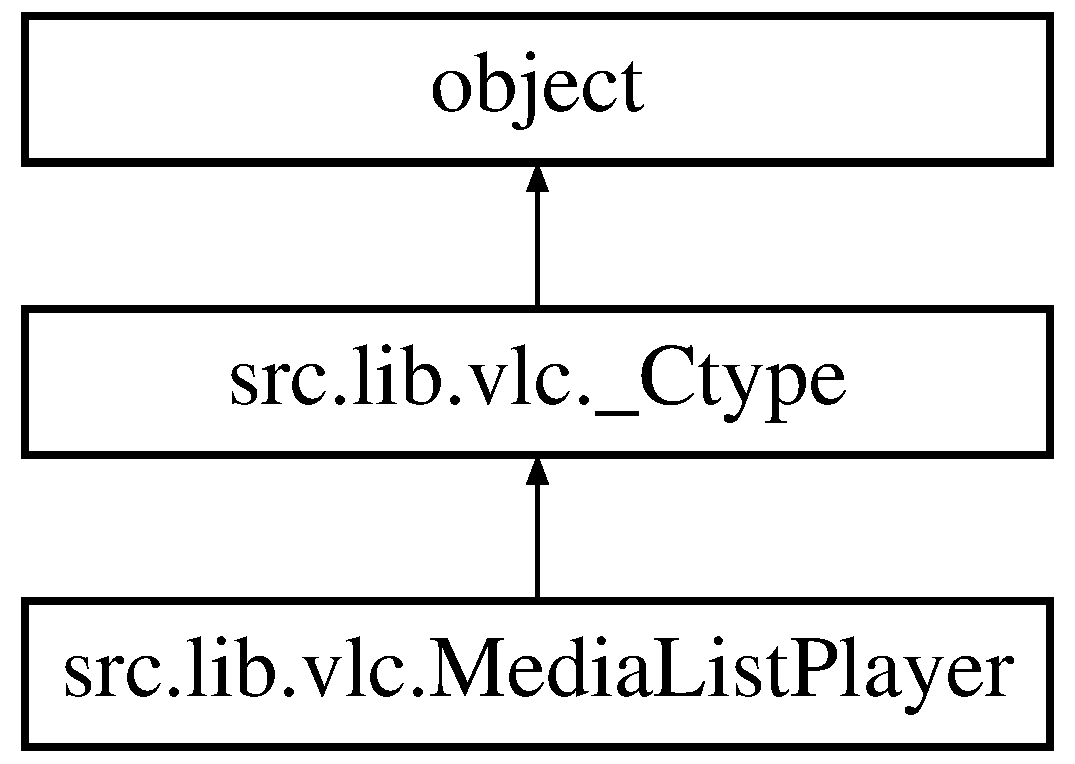
\includegraphics[height=3.000000cm]{classsrc_1_1lib_1_1vlc_1_1MediaListPlayer}
\end{center}
\end{figure}
\subsection*{Public Member Functions}
\begin{DoxyCompactItemize}
\item 
def \hyperlink{classsrc_1_1lib_1_1vlc_1_1MediaListPlayer_a6a00ba884fbd12bd50e925900ac9afdd}{\+\_\+\+\_\+new\+\_\+\+\_\+}
\item 
def \hyperlink{classsrc_1_1lib_1_1vlc_1_1MediaListPlayer_a7cba140bab9b134c069e6c643ea6e4b8}{get\+\_\+instance} (self)
\item 
def \hyperlink{classsrc_1_1lib_1_1vlc_1_1MediaListPlayer_ae091f90b3e798db3d39f56a05036a8c4}{release} (self)
\item 
def \hyperlink{classsrc_1_1lib_1_1vlc_1_1MediaListPlayer_a9a6aad5a53000b64e727e3d0979d775e}{retain} (self)
\item 
def \hyperlink{classsrc_1_1lib_1_1vlc_1_1MediaListPlayer_a6825e34f893a0408d8bf64b268badcad}{event\+\_\+manager} (self)
\item 
def \hyperlink{classsrc_1_1lib_1_1vlc_1_1MediaListPlayer_a0e79bb23a5b9f95e8bc087a645f105a2}{set\+\_\+media\+\_\+player} (self, p\+\_\+mi)
\item 
def \hyperlink{classsrc_1_1lib_1_1vlc_1_1MediaListPlayer_a1cfc33bae19366938758bcdbc2fb9aa4}{set\+\_\+media\+\_\+list} (self, p\+\_\+mlist)
\item 
def \hyperlink{classsrc_1_1lib_1_1vlc_1_1MediaListPlayer_a7a0586b4921dd11d98afe4ae955ca1dd}{play} (self)
\item 
def \hyperlink{classsrc_1_1lib_1_1vlc_1_1MediaListPlayer_ab55560ffca721b03629f4607e0d69bbc}{pause} (self)
\item 
def \hyperlink{classsrc_1_1lib_1_1vlc_1_1MediaListPlayer_a7de79f0992d43dc68107ff4667048cd2}{is\+\_\+playing} (self)
\item 
def \hyperlink{classsrc_1_1lib_1_1vlc_1_1MediaListPlayer_adfc9fdb1f5e72a681eb6fa7c28544543}{get\+\_\+state} (self)
\item 
def \hyperlink{classsrc_1_1lib_1_1vlc_1_1MediaListPlayer_abfbdf506fb948a060712692f5ac3edae}{play\+\_\+item\+\_\+at\+\_\+index} (self, i\+\_\+index)
\item 
def \hyperlink{classsrc_1_1lib_1_1vlc_1_1MediaListPlayer_a0dd0daddbae8badbdbafbdbc1587b1f8}{\+\_\+\+\_\+getitem\+\_\+\+\_\+} (self, i)
\item 
def \hyperlink{classsrc_1_1lib_1_1vlc_1_1MediaListPlayer_aad30dcdd7cb8147b4033bdff3ab1fbad}{\+\_\+\+\_\+iter\+\_\+\+\_\+} (self)
\item 
def \hyperlink{classsrc_1_1lib_1_1vlc_1_1MediaListPlayer_a44902ba2903b067ab0446279fa4dae8d}{play\+\_\+item} (self, p\+\_\+md)
\item 
def \hyperlink{classsrc_1_1lib_1_1vlc_1_1MediaListPlayer_a8cc91496e6bd7bca30ace12b2b907dbd}{stop} (self)
\item 
def \hyperlink{classsrc_1_1lib_1_1vlc_1_1MediaListPlayer_a26a5101a6c719b6d77fe1146f4bcbb7e}{next} (self)
\item 
def \hyperlink{classsrc_1_1lib_1_1vlc_1_1MediaListPlayer_a4c441b0700a6071372240b781877b3ff}{previous} (self)
\item 
def \hyperlink{classsrc_1_1lib_1_1vlc_1_1MediaListPlayer_a40dfc286beb6b4f44780bfefa6898fe7}{set\+\_\+playback\+\_\+mode} (self, e\+\_\+mode)
\end{DoxyCompactItemize}
\subsection*{Additional Inherited Members}


\subsection{Detailed Description}
\begin{DoxyVerb}Create a new MediaListPlayer instance.

It may take as parameter either:
  - a vlc.Instance
  - nothing\end{DoxyVerb}
 

\subsection{Member Function Documentation}
\hypertarget{classsrc_1_1lib_1_1vlc_1_1MediaListPlayer_a0dd0daddbae8badbdbafbdbc1587b1f8}{}\index{src\+::lib\+::vlc\+::\+Media\+List\+Player@{src\+::lib\+::vlc\+::\+Media\+List\+Player}!\+\_\+\+\_\+getitem\+\_\+\+\_\+@{\+\_\+\+\_\+getitem\+\_\+\+\_\+}}
\index{\+\_\+\+\_\+getitem\+\_\+\+\_\+@{\+\_\+\+\_\+getitem\+\_\+\+\_\+}!src\+::lib\+::vlc\+::\+Media\+List\+Player@{src\+::lib\+::vlc\+::\+Media\+List\+Player}}
\subsubsection[{\+\_\+\+\_\+getitem\+\_\+\+\_\+}]{\setlength{\rightskip}{0pt plus 5cm}def src.\+lib.\+vlc.\+Media\+List\+Player.\+\_\+\+\_\+getitem\+\_\+\+\_\+ (
\begin{DoxyParamCaption}
\item[{}]{self, }
\item[{}]{i}
\end{DoxyParamCaption}
)}\label{classsrc_1_1lib_1_1vlc_1_1MediaListPlayer_a0dd0daddbae8badbdbafbdbc1587b1f8}
\hypertarget{classsrc_1_1lib_1_1vlc_1_1MediaListPlayer_aad30dcdd7cb8147b4033bdff3ab1fbad}{}\index{src\+::lib\+::vlc\+::\+Media\+List\+Player@{src\+::lib\+::vlc\+::\+Media\+List\+Player}!\+\_\+\+\_\+iter\+\_\+\+\_\+@{\+\_\+\+\_\+iter\+\_\+\+\_\+}}
\index{\+\_\+\+\_\+iter\+\_\+\+\_\+@{\+\_\+\+\_\+iter\+\_\+\+\_\+}!src\+::lib\+::vlc\+::\+Media\+List\+Player@{src\+::lib\+::vlc\+::\+Media\+List\+Player}}
\subsubsection[{\+\_\+\+\_\+iter\+\_\+\+\_\+}]{\setlength{\rightskip}{0pt plus 5cm}def src.\+lib.\+vlc.\+Media\+List\+Player.\+\_\+\+\_\+iter\+\_\+\+\_\+ (
\begin{DoxyParamCaption}
\item[{}]{self}
\end{DoxyParamCaption}
)}\label{classsrc_1_1lib_1_1vlc_1_1MediaListPlayer_aad30dcdd7cb8147b4033bdff3ab1fbad}
\hypertarget{classsrc_1_1lib_1_1vlc_1_1MediaListPlayer_a6a00ba884fbd12bd50e925900ac9afdd}{}\index{src\+::lib\+::vlc\+::\+Media\+List\+Player@{src\+::lib\+::vlc\+::\+Media\+List\+Player}!\+\_\+\+\_\+new\+\_\+\+\_\+@{\+\_\+\+\_\+new\+\_\+\+\_\+}}
\index{\+\_\+\+\_\+new\+\_\+\+\_\+@{\+\_\+\+\_\+new\+\_\+\+\_\+}!src\+::lib\+::vlc\+::\+Media\+List\+Player@{src\+::lib\+::vlc\+::\+Media\+List\+Player}}
\subsubsection[{\+\_\+\+\_\+new\+\_\+\+\_\+}]{\setlength{\rightskip}{0pt plus 5cm}def src.\+lib.\+vlc.\+Media\+List\+Player.\+\_\+\+\_\+new\+\_\+\+\_\+ (
\begin{DoxyParamCaption}
\item[{}]{cls, }
\item[{}]{arg = {\ttfamily None}}
\end{DoxyParamCaption}
)}\label{classsrc_1_1lib_1_1vlc_1_1MediaListPlayer_a6a00ba884fbd12bd50e925900ac9afdd}
\hypertarget{classsrc_1_1lib_1_1vlc_1_1MediaListPlayer_a6825e34f893a0408d8bf64b268badcad}{}\index{src\+::lib\+::vlc\+::\+Media\+List\+Player@{src\+::lib\+::vlc\+::\+Media\+List\+Player}!event\+\_\+manager@{event\+\_\+manager}}
\index{event\+\_\+manager@{event\+\_\+manager}!src\+::lib\+::vlc\+::\+Media\+List\+Player@{src\+::lib\+::vlc\+::\+Media\+List\+Player}}
\subsubsection[{event\+\_\+manager}]{\setlength{\rightskip}{0pt plus 5cm}def src.\+lib.\+vlc.\+Media\+List\+Player.\+event\+\_\+manager (
\begin{DoxyParamCaption}
\item[{}]{self}
\end{DoxyParamCaption}
)}\label{classsrc_1_1lib_1_1vlc_1_1MediaListPlayer_a6825e34f893a0408d8bf64b268badcad}
\begin{DoxyVerb}Return the event manager of this media_list_player.
@return: the event manager.
\end{DoxyVerb}
 \hypertarget{classsrc_1_1lib_1_1vlc_1_1MediaListPlayer_a7cba140bab9b134c069e6c643ea6e4b8}{}\index{src\+::lib\+::vlc\+::\+Media\+List\+Player@{src\+::lib\+::vlc\+::\+Media\+List\+Player}!get\+\_\+instance@{get\+\_\+instance}}
\index{get\+\_\+instance@{get\+\_\+instance}!src\+::lib\+::vlc\+::\+Media\+List\+Player@{src\+::lib\+::vlc\+::\+Media\+List\+Player}}
\subsubsection[{get\+\_\+instance}]{\setlength{\rightskip}{0pt plus 5cm}def src.\+lib.\+vlc.\+Media\+List\+Player.\+get\+\_\+instance (
\begin{DoxyParamCaption}
\item[{}]{self}
\end{DoxyParamCaption}
)}\label{classsrc_1_1lib_1_1vlc_1_1MediaListPlayer_a7cba140bab9b134c069e6c643ea6e4b8}
\begin{DoxyVerb}Return the associated Instance.
\end{DoxyVerb}
 \hypertarget{classsrc_1_1lib_1_1vlc_1_1MediaListPlayer_adfc9fdb1f5e72a681eb6fa7c28544543}{}\index{src\+::lib\+::vlc\+::\+Media\+List\+Player@{src\+::lib\+::vlc\+::\+Media\+List\+Player}!get\+\_\+state@{get\+\_\+state}}
\index{get\+\_\+state@{get\+\_\+state}!src\+::lib\+::vlc\+::\+Media\+List\+Player@{src\+::lib\+::vlc\+::\+Media\+List\+Player}}
\subsubsection[{get\+\_\+state}]{\setlength{\rightskip}{0pt plus 5cm}def src.\+lib.\+vlc.\+Media\+List\+Player.\+get\+\_\+state (
\begin{DoxyParamCaption}
\item[{}]{self}
\end{DoxyParamCaption}
)}\label{classsrc_1_1lib_1_1vlc_1_1MediaListPlayer_adfc9fdb1f5e72a681eb6fa7c28544543}
\begin{DoxyVerb}Get current libvlc_state of media list player.
@return: libvlc_state_t for media list player.
\end{DoxyVerb}
 \hypertarget{classsrc_1_1lib_1_1vlc_1_1MediaListPlayer_a7de79f0992d43dc68107ff4667048cd2}{}\index{src\+::lib\+::vlc\+::\+Media\+List\+Player@{src\+::lib\+::vlc\+::\+Media\+List\+Player}!is\+\_\+playing@{is\+\_\+playing}}
\index{is\+\_\+playing@{is\+\_\+playing}!src\+::lib\+::vlc\+::\+Media\+List\+Player@{src\+::lib\+::vlc\+::\+Media\+List\+Player}}
\subsubsection[{is\+\_\+playing}]{\setlength{\rightskip}{0pt plus 5cm}def src.\+lib.\+vlc.\+Media\+List\+Player.\+is\+\_\+playing (
\begin{DoxyParamCaption}
\item[{}]{self}
\end{DoxyParamCaption}
)}\label{classsrc_1_1lib_1_1vlc_1_1MediaListPlayer_a7de79f0992d43dc68107ff4667048cd2}
\begin{DoxyVerb}Is media list playing?
@return: true for playing and false for not playing \libvlc_return_bool.
\end{DoxyVerb}
 \hypertarget{classsrc_1_1lib_1_1vlc_1_1MediaListPlayer_a26a5101a6c719b6d77fe1146f4bcbb7e}{}\index{src\+::lib\+::vlc\+::\+Media\+List\+Player@{src\+::lib\+::vlc\+::\+Media\+List\+Player}!next@{next}}
\index{next@{next}!src\+::lib\+::vlc\+::\+Media\+List\+Player@{src\+::lib\+::vlc\+::\+Media\+List\+Player}}
\subsubsection[{next}]{\setlength{\rightskip}{0pt plus 5cm}def src.\+lib.\+vlc.\+Media\+List\+Player.\+next (
\begin{DoxyParamCaption}
\item[{}]{self}
\end{DoxyParamCaption}
)}\label{classsrc_1_1lib_1_1vlc_1_1MediaListPlayer_a26a5101a6c719b6d77fe1146f4bcbb7e}
\begin{DoxyVerb}Play next item from media list.
@return: 0 upon success -1 if there is no next item.
\end{DoxyVerb}
 \hypertarget{classsrc_1_1lib_1_1vlc_1_1MediaListPlayer_ab55560ffca721b03629f4607e0d69bbc}{}\index{src\+::lib\+::vlc\+::\+Media\+List\+Player@{src\+::lib\+::vlc\+::\+Media\+List\+Player}!pause@{pause}}
\index{pause@{pause}!src\+::lib\+::vlc\+::\+Media\+List\+Player@{src\+::lib\+::vlc\+::\+Media\+List\+Player}}
\subsubsection[{pause}]{\setlength{\rightskip}{0pt plus 5cm}def src.\+lib.\+vlc.\+Media\+List\+Player.\+pause (
\begin{DoxyParamCaption}
\item[{}]{self}
\end{DoxyParamCaption}
)}\label{classsrc_1_1lib_1_1vlc_1_1MediaListPlayer_ab55560ffca721b03629f4607e0d69bbc}
\begin{DoxyVerb}Pause media list.
\end{DoxyVerb}
 \hypertarget{classsrc_1_1lib_1_1vlc_1_1MediaListPlayer_a7a0586b4921dd11d98afe4ae955ca1dd}{}\index{src\+::lib\+::vlc\+::\+Media\+List\+Player@{src\+::lib\+::vlc\+::\+Media\+List\+Player}!play@{play}}
\index{play@{play}!src\+::lib\+::vlc\+::\+Media\+List\+Player@{src\+::lib\+::vlc\+::\+Media\+List\+Player}}
\subsubsection[{play}]{\setlength{\rightskip}{0pt plus 5cm}def src.\+lib.\+vlc.\+Media\+List\+Player.\+play (
\begin{DoxyParamCaption}
\item[{}]{self}
\end{DoxyParamCaption}
)}\label{classsrc_1_1lib_1_1vlc_1_1MediaListPlayer_a7a0586b4921dd11d98afe4ae955ca1dd}
\begin{DoxyVerb}Play media list.
\end{DoxyVerb}
 \hypertarget{classsrc_1_1lib_1_1vlc_1_1MediaListPlayer_a44902ba2903b067ab0446279fa4dae8d}{}\index{src\+::lib\+::vlc\+::\+Media\+List\+Player@{src\+::lib\+::vlc\+::\+Media\+List\+Player}!play\+\_\+item@{play\+\_\+item}}
\index{play\+\_\+item@{play\+\_\+item}!src\+::lib\+::vlc\+::\+Media\+List\+Player@{src\+::lib\+::vlc\+::\+Media\+List\+Player}}
\subsubsection[{play\+\_\+item}]{\setlength{\rightskip}{0pt plus 5cm}def src.\+lib.\+vlc.\+Media\+List\+Player.\+play\+\_\+item (
\begin{DoxyParamCaption}
\item[{}]{self, }
\item[{}]{p\+\_\+md}
\end{DoxyParamCaption}
)}\label{classsrc_1_1lib_1_1vlc_1_1MediaListPlayer_a44902ba2903b067ab0446279fa4dae8d}
\begin{DoxyVerb}Play the given media item.
@param p_md: the media instance.
@return: 0 upon success, -1 if the media is not part of the media list.
\end{DoxyVerb}
 \hypertarget{classsrc_1_1lib_1_1vlc_1_1MediaListPlayer_abfbdf506fb948a060712692f5ac3edae}{}\index{src\+::lib\+::vlc\+::\+Media\+List\+Player@{src\+::lib\+::vlc\+::\+Media\+List\+Player}!play\+\_\+item\+\_\+at\+\_\+index@{play\+\_\+item\+\_\+at\+\_\+index}}
\index{play\+\_\+item\+\_\+at\+\_\+index@{play\+\_\+item\+\_\+at\+\_\+index}!src\+::lib\+::vlc\+::\+Media\+List\+Player@{src\+::lib\+::vlc\+::\+Media\+List\+Player}}
\subsubsection[{play\+\_\+item\+\_\+at\+\_\+index}]{\setlength{\rightskip}{0pt plus 5cm}def src.\+lib.\+vlc.\+Media\+List\+Player.\+play\+\_\+item\+\_\+at\+\_\+index (
\begin{DoxyParamCaption}
\item[{}]{self, }
\item[{}]{i\+\_\+index}
\end{DoxyParamCaption}
)}\label{classsrc_1_1lib_1_1vlc_1_1MediaListPlayer_abfbdf506fb948a060712692f5ac3edae}
\begin{DoxyVerb}Play media list item at position index.
@param i_index: index in media list to play.
@return: 0 upon success -1 if the item wasn't found.
\end{DoxyVerb}
 \hypertarget{classsrc_1_1lib_1_1vlc_1_1MediaListPlayer_a4c441b0700a6071372240b781877b3ff}{}\index{src\+::lib\+::vlc\+::\+Media\+List\+Player@{src\+::lib\+::vlc\+::\+Media\+List\+Player}!previous@{previous}}
\index{previous@{previous}!src\+::lib\+::vlc\+::\+Media\+List\+Player@{src\+::lib\+::vlc\+::\+Media\+List\+Player}}
\subsubsection[{previous}]{\setlength{\rightskip}{0pt plus 5cm}def src.\+lib.\+vlc.\+Media\+List\+Player.\+previous (
\begin{DoxyParamCaption}
\item[{}]{self}
\end{DoxyParamCaption}
)}\label{classsrc_1_1lib_1_1vlc_1_1MediaListPlayer_a4c441b0700a6071372240b781877b3ff}
\begin{DoxyVerb}Play previous item from media list.
@return: 0 upon success -1 if there is no previous item.
\end{DoxyVerb}
 \hypertarget{classsrc_1_1lib_1_1vlc_1_1MediaListPlayer_ae091f90b3e798db3d39f56a05036a8c4}{}\index{src\+::lib\+::vlc\+::\+Media\+List\+Player@{src\+::lib\+::vlc\+::\+Media\+List\+Player}!release@{release}}
\index{release@{release}!src\+::lib\+::vlc\+::\+Media\+List\+Player@{src\+::lib\+::vlc\+::\+Media\+List\+Player}}
\subsubsection[{release}]{\setlength{\rightskip}{0pt plus 5cm}def src.\+lib.\+vlc.\+Media\+List\+Player.\+release (
\begin{DoxyParamCaption}
\item[{}]{self}
\end{DoxyParamCaption}
)}\label{classsrc_1_1lib_1_1vlc_1_1MediaListPlayer_ae091f90b3e798db3d39f56a05036a8c4}
\begin{DoxyVerb}Release a media_list_player after use
Decrement the reference count of a media player object. If the
reference count is 0, then L{release}() will
release the media player object. If the media player object
has been released, then it should not be used again.
\end{DoxyVerb}
 \hypertarget{classsrc_1_1lib_1_1vlc_1_1MediaListPlayer_a9a6aad5a53000b64e727e3d0979d775e}{}\index{src\+::lib\+::vlc\+::\+Media\+List\+Player@{src\+::lib\+::vlc\+::\+Media\+List\+Player}!retain@{retain}}
\index{retain@{retain}!src\+::lib\+::vlc\+::\+Media\+List\+Player@{src\+::lib\+::vlc\+::\+Media\+List\+Player}}
\subsubsection[{retain}]{\setlength{\rightskip}{0pt plus 5cm}def src.\+lib.\+vlc.\+Media\+List\+Player.\+retain (
\begin{DoxyParamCaption}
\item[{}]{self}
\end{DoxyParamCaption}
)}\label{classsrc_1_1lib_1_1vlc_1_1MediaListPlayer_a9a6aad5a53000b64e727e3d0979d775e}
\begin{DoxyVerb}Retain a reference to a media player list object. Use
L{release}() to decrement reference count.
\end{DoxyVerb}
 \hypertarget{classsrc_1_1lib_1_1vlc_1_1MediaListPlayer_a1cfc33bae19366938758bcdbc2fb9aa4}{}\index{src\+::lib\+::vlc\+::\+Media\+List\+Player@{src\+::lib\+::vlc\+::\+Media\+List\+Player}!set\+\_\+media\+\_\+list@{set\+\_\+media\+\_\+list}}
\index{set\+\_\+media\+\_\+list@{set\+\_\+media\+\_\+list}!src\+::lib\+::vlc\+::\+Media\+List\+Player@{src\+::lib\+::vlc\+::\+Media\+List\+Player}}
\subsubsection[{set\+\_\+media\+\_\+list}]{\setlength{\rightskip}{0pt plus 5cm}def src.\+lib.\+vlc.\+Media\+List\+Player.\+set\+\_\+media\+\_\+list (
\begin{DoxyParamCaption}
\item[{}]{self, }
\item[{}]{p\+\_\+mlist}
\end{DoxyParamCaption}
)}\label{classsrc_1_1lib_1_1vlc_1_1MediaListPlayer_a1cfc33bae19366938758bcdbc2fb9aa4}
\begin{DoxyVerb}Set the media list associated with the player.
@param p_mlist: list of media.
\end{DoxyVerb}
 \hypertarget{classsrc_1_1lib_1_1vlc_1_1MediaListPlayer_a0e79bb23a5b9f95e8bc087a645f105a2}{}\index{src\+::lib\+::vlc\+::\+Media\+List\+Player@{src\+::lib\+::vlc\+::\+Media\+List\+Player}!set\+\_\+media\+\_\+player@{set\+\_\+media\+\_\+player}}
\index{set\+\_\+media\+\_\+player@{set\+\_\+media\+\_\+player}!src\+::lib\+::vlc\+::\+Media\+List\+Player@{src\+::lib\+::vlc\+::\+Media\+List\+Player}}
\subsubsection[{set\+\_\+media\+\_\+player}]{\setlength{\rightskip}{0pt plus 5cm}def src.\+lib.\+vlc.\+Media\+List\+Player.\+set\+\_\+media\+\_\+player (
\begin{DoxyParamCaption}
\item[{}]{self, }
\item[{}]{p\+\_\+mi}
\end{DoxyParamCaption}
)}\label{classsrc_1_1lib_1_1vlc_1_1MediaListPlayer_a0e79bb23a5b9f95e8bc087a645f105a2}
\begin{DoxyVerb}Replace media player in media_list_player with this instance.
@param p_mi: media player instance.
\end{DoxyVerb}
 \hypertarget{classsrc_1_1lib_1_1vlc_1_1MediaListPlayer_a40dfc286beb6b4f44780bfefa6898fe7}{}\index{src\+::lib\+::vlc\+::\+Media\+List\+Player@{src\+::lib\+::vlc\+::\+Media\+List\+Player}!set\+\_\+playback\+\_\+mode@{set\+\_\+playback\+\_\+mode}}
\index{set\+\_\+playback\+\_\+mode@{set\+\_\+playback\+\_\+mode}!src\+::lib\+::vlc\+::\+Media\+List\+Player@{src\+::lib\+::vlc\+::\+Media\+List\+Player}}
\subsubsection[{set\+\_\+playback\+\_\+mode}]{\setlength{\rightskip}{0pt plus 5cm}def src.\+lib.\+vlc.\+Media\+List\+Player.\+set\+\_\+playback\+\_\+mode (
\begin{DoxyParamCaption}
\item[{}]{self, }
\item[{}]{e\+\_\+mode}
\end{DoxyParamCaption}
)}\label{classsrc_1_1lib_1_1vlc_1_1MediaListPlayer_a40dfc286beb6b4f44780bfefa6898fe7}
\begin{DoxyVerb}Sets the playback mode for the playlist.
@param e_mode: playback mode specification.
\end{DoxyVerb}
 \hypertarget{classsrc_1_1lib_1_1vlc_1_1MediaListPlayer_a8cc91496e6bd7bca30ace12b2b907dbd}{}\index{src\+::lib\+::vlc\+::\+Media\+List\+Player@{src\+::lib\+::vlc\+::\+Media\+List\+Player}!stop@{stop}}
\index{stop@{stop}!src\+::lib\+::vlc\+::\+Media\+List\+Player@{src\+::lib\+::vlc\+::\+Media\+List\+Player}}
\subsubsection[{stop}]{\setlength{\rightskip}{0pt plus 5cm}def src.\+lib.\+vlc.\+Media\+List\+Player.\+stop (
\begin{DoxyParamCaption}
\item[{}]{self}
\end{DoxyParamCaption}
)}\label{classsrc_1_1lib_1_1vlc_1_1MediaListPlayer_a8cc91496e6bd7bca30ace12b2b907dbd}
\begin{DoxyVerb}Stop playing media list.
\end{DoxyVerb}
 

The documentation for this class was generated from the following file\+:\begin{DoxyCompactItemize}
\item 
src/lib/\hyperlink{vlc_8py}{vlc.\+py}\end{DoxyCompactItemize}

\hypertarget{classsrc_1_1lib_1_1vlc_1_1MediaPlayer}{}\section{src.\+lib.\+vlc.\+Media\+Player Class Reference}
\label{classsrc_1_1lib_1_1vlc_1_1MediaPlayer}\index{src.\+lib.\+vlc.\+Media\+Player@{src.\+lib.\+vlc.\+Media\+Player}}
Inheritance diagram for src.\+lib.\+vlc.\+Media\+Player\+:\begin{figure}[H]
\begin{center}
\leavevmode
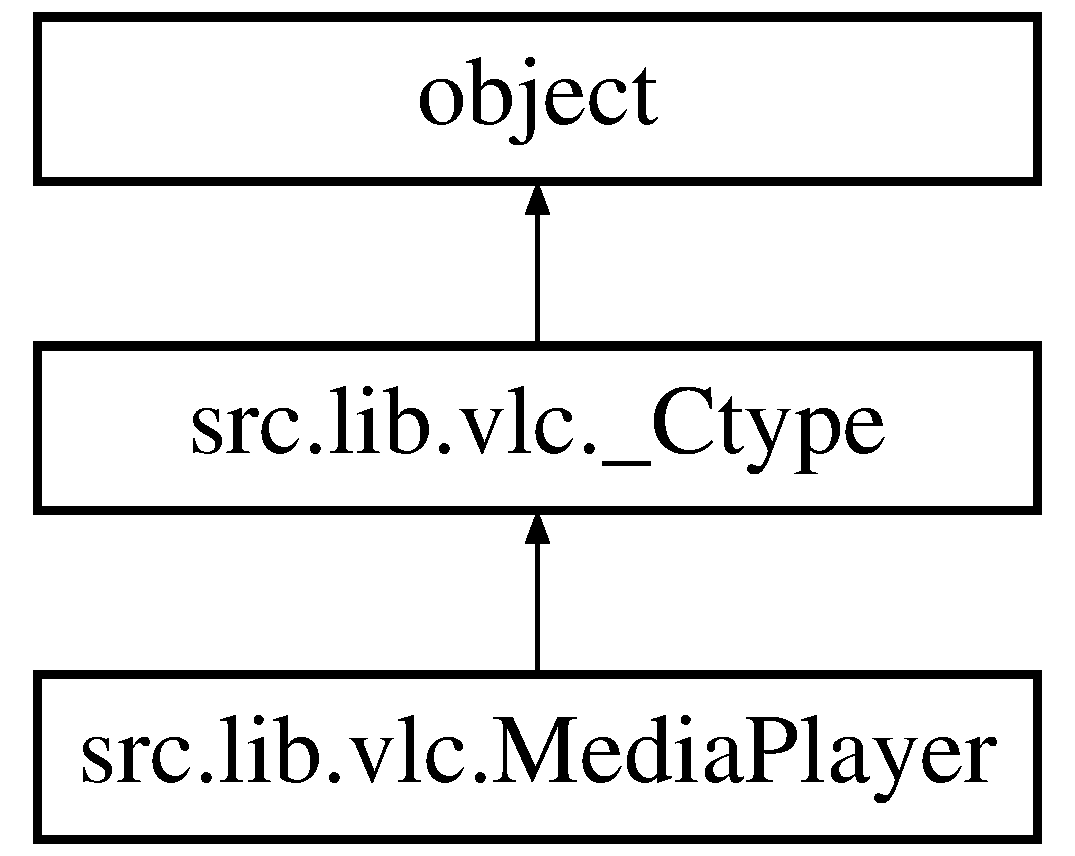
\includegraphics[height=3.000000cm]{classsrc_1_1lib_1_1vlc_1_1MediaPlayer}
\end{center}
\end{figure}
\subsection*{Public Member Functions}
\begin{DoxyCompactItemize}
\item 
def \hyperlink{classsrc_1_1lib_1_1vlc_1_1MediaPlayer_ac13f8b11bd1dbb0779d79a8e5b6f7213}{\+\_\+\+\_\+new\+\_\+\+\_\+} (cls, args)
\item 
def \hyperlink{classsrc_1_1lib_1_1vlc_1_1MediaPlayer_a264eda1ac9755ec3628a1aa2c0380278}{get\+\_\+instance} (self)
\item 
def \hyperlink{classsrc_1_1lib_1_1vlc_1_1MediaPlayer_a94ebfbaa9c96105656c8353a507e85ac}{set\+\_\+mrl} (self, mrl, options)
\item 
def \hyperlink{classsrc_1_1lib_1_1vlc_1_1MediaPlayer_afc33dc5b48f9455259acd856d47578f5}{video\+\_\+get\+\_\+spu\+\_\+description} (self)
\item 
def \hyperlink{classsrc_1_1lib_1_1vlc_1_1MediaPlayer_a6405c62a60af867bc5d13f4cc40876d2}{video\+\_\+get\+\_\+title\+\_\+description} (self)
\item 
def \hyperlink{classsrc_1_1lib_1_1vlc_1_1MediaPlayer_aafc25cfcae05b82c8558ad14724f727f}{video\+\_\+get\+\_\+chapter\+\_\+description} (self, title)
\item 
def \hyperlink{classsrc_1_1lib_1_1vlc_1_1MediaPlayer_a9550de3d65aac8f7f2c122ee6046eba2}{video\+\_\+get\+\_\+track\+\_\+description} (self)
\item 
def \hyperlink{classsrc_1_1lib_1_1vlc_1_1MediaPlayer_a1f368380024537d51f095f265f5f8dea}{audio\+\_\+get\+\_\+track\+\_\+description} (self)
\item 
def \hyperlink{classsrc_1_1lib_1_1vlc_1_1MediaPlayer_af3f0fc8cb2d9dd363c9953759570f39f}{video\+\_\+get\+\_\+size}
\item 
def \hyperlink{classsrc_1_1lib_1_1vlc_1_1MediaPlayer_a11f19ca6cdd8581c4b270327ff171a75}{set\+\_\+hwnd} (self, drawable)
\item 
def \hyperlink{classsrc_1_1lib_1_1vlc_1_1MediaPlayer_a7f2dcd26949bd60b59b52525f203f5dc}{video\+\_\+get\+\_\+width}
\item 
def \hyperlink{classsrc_1_1lib_1_1vlc_1_1MediaPlayer_ab57308d53debfea51273f7a8d2650f37}{video\+\_\+get\+\_\+height}
\item 
def \hyperlink{classsrc_1_1lib_1_1vlc_1_1MediaPlayer_a566fb82157c233b0e0b00f3cd54386b1}{video\+\_\+get\+\_\+cursor}
\item 
def \hyperlink{classsrc_1_1lib_1_1vlc_1_1MediaPlayer_aa1a2f85b506a01492eecfa3655211d89}{release} (self)
\item 
def \hyperlink{classsrc_1_1lib_1_1vlc_1_1MediaPlayer_ac0121fad637351ed9aeab49b88ed88be}{retain} (self)
\item 
def \hyperlink{classsrc_1_1lib_1_1vlc_1_1MediaPlayer_a45a307fa37ff9bbeec84124508726653}{set\+\_\+media} (self, p\+\_\+md)
\item 
def \hyperlink{classsrc_1_1lib_1_1vlc_1_1MediaPlayer_aec7d3bca8d27830f54f114602acae3a9}{get\+\_\+media} (self)
\item 
def \hyperlink{classsrc_1_1lib_1_1vlc_1_1MediaPlayer_a9b5c63ec99ddbbed2dc0a34cbcbc6891}{event\+\_\+manager} (self)
\item 
def \hyperlink{classsrc_1_1lib_1_1vlc_1_1MediaPlayer_a05082c680fd1bcdc16eb37af9e68b035}{is\+\_\+playing} (self)
\item 
def \hyperlink{classsrc_1_1lib_1_1vlc_1_1MediaPlayer_a4ee719f902692b68bb0c2f8e6e6bc40d}{play} (self)
\item 
def \hyperlink{classsrc_1_1lib_1_1vlc_1_1MediaPlayer_a7a22f40a01f996b374fccb68daf17f89}{set\+\_\+pause} (self, do\+\_\+pause)
\item 
def \hyperlink{classsrc_1_1lib_1_1vlc_1_1MediaPlayer_acaf59e59e5945245a78397df9c98b177}{pause} (self)
\item 
def \hyperlink{classsrc_1_1lib_1_1vlc_1_1MediaPlayer_a0843d58c2e37d5d9cb48cc06974a515e}{stop} (self)
\item 
def \hyperlink{classsrc_1_1lib_1_1vlc_1_1MediaPlayer_a313c0554d2c88f2688872a00da329752}{video\+\_\+set\+\_\+format} (self, chroma, width, height, pitch)
\item 
def \hyperlink{classsrc_1_1lib_1_1vlc_1_1MediaPlayer_a687928ea3d9fb590c0d0056887c71556}{set\+\_\+nsobject} (self, drawable)
\item 
def \hyperlink{classsrc_1_1lib_1_1vlc_1_1MediaPlayer_ac2976c87f9e1d84603ddb942ce277c4c}{get\+\_\+nsobject} (self)
\item 
def \hyperlink{classsrc_1_1lib_1_1vlc_1_1MediaPlayer_a07f411e0da32789ae56c94f11128ddac}{set\+\_\+agl} (self, drawable)
\item 
def \hyperlink{classsrc_1_1lib_1_1vlc_1_1MediaPlayer_a7cca20069084bf8450325c0def66e5d4}{get\+\_\+agl} (self)
\item 
def \hyperlink{classsrc_1_1lib_1_1vlc_1_1MediaPlayer_a8f1c62c5fe29fad1369b0d22825aa378}{set\+\_\+xwindow} (self, drawable)
\item 
def \hyperlink{classsrc_1_1lib_1_1vlc_1_1MediaPlayer_af055577c7417fcac511e59df093391bb}{get\+\_\+xwindow} (self)
\item 
def \hyperlink{classsrc_1_1lib_1_1vlc_1_1MediaPlayer_a012c90b9498719b07fd166c29abc0e8d}{get\+\_\+hwnd} (self)
\item 
def \hyperlink{classsrc_1_1lib_1_1vlc_1_1MediaPlayer_a674aacbc9b080a61e3d440c3a498a8d7}{audio\+\_\+set\+\_\+format} (self, format, rate, channels)
\item 
def \hyperlink{classsrc_1_1lib_1_1vlc_1_1MediaPlayer_a373c8d8f499288284ae12a2aa73ce96d}{get\+\_\+length} (self)
\item 
def \hyperlink{classsrc_1_1lib_1_1vlc_1_1MediaPlayer_ad103f94a34e009402852d7e00a3d6cd6}{get\+\_\+time} (self)
\item 
def \hyperlink{classsrc_1_1lib_1_1vlc_1_1MediaPlayer_a18efdd20988db9c578f175270c169d54}{set\+\_\+time} (self, i\+\_\+time)
\item 
def \hyperlink{classsrc_1_1lib_1_1vlc_1_1MediaPlayer_a9b72ddf97057a5c3443635985dde1389}{get\+\_\+position} (self)
\item 
def \hyperlink{classsrc_1_1lib_1_1vlc_1_1MediaPlayer_a9f80dfc502b5abf41c01a6c7eef740e3}{set\+\_\+position} (self, f\+\_\+pos)
\item 
def \hyperlink{classsrc_1_1lib_1_1vlc_1_1MediaPlayer_adecb86a817d32db7ef243bfab6705ec5}{set\+\_\+chapter} (self, i\+\_\+chapter)
\item 
def \hyperlink{classsrc_1_1lib_1_1vlc_1_1MediaPlayer_a58f479b2e275a53161508ee2b266cde9}{get\+\_\+chapter} (self)
\item 
def \hyperlink{classsrc_1_1lib_1_1vlc_1_1MediaPlayer_aa7031d6e26e432e8bfeab2f7f38ef854}{get\+\_\+chapter\+\_\+count} (self)
\item 
def \hyperlink{classsrc_1_1lib_1_1vlc_1_1MediaPlayer_a17a09ea748e103c89a691d12b78e20bd}{will\+\_\+play} (self)
\item 
def \hyperlink{classsrc_1_1lib_1_1vlc_1_1MediaPlayer_a46b17d5e90d15d4b5722953d96430dc3}{get\+\_\+chapter\+\_\+count\+\_\+for\+\_\+title} (self, i\+\_\+title)
\item 
def \hyperlink{classsrc_1_1lib_1_1vlc_1_1MediaPlayer_ab6b826a8b4aaf135ef60114e26779697}{set\+\_\+title} (self, i\+\_\+title)
\item 
def \hyperlink{classsrc_1_1lib_1_1vlc_1_1MediaPlayer_a37919d4c470acbf72d79c87f34bcedea}{get\+\_\+title} (self)
\item 
def \hyperlink{classsrc_1_1lib_1_1vlc_1_1MediaPlayer_a95e6795e0f76b9cb8579a299e6c2b24b}{get\+\_\+title\+\_\+count} (self)
\item 
def \hyperlink{classsrc_1_1lib_1_1vlc_1_1MediaPlayer_a72f5ea15c85220d6246858a30d20e26a}{previous\+\_\+chapter} (self)
\item 
def \hyperlink{classsrc_1_1lib_1_1vlc_1_1MediaPlayer_a4a85fc790507f37298912bfc325ba0b2}{next\+\_\+chapter} (self)
\item 
def \hyperlink{classsrc_1_1lib_1_1vlc_1_1MediaPlayer_a5c5ed3b44219e7328c0e57359bd84bfc}{get\+\_\+rate} (self)
\item 
def \hyperlink{classsrc_1_1lib_1_1vlc_1_1MediaPlayer_a20747e5bcf1868c13a408fb3eb457a3d}{set\+\_\+rate} (self, rate)
\item 
def \hyperlink{classsrc_1_1lib_1_1vlc_1_1MediaPlayer_a02a04a9e4326bf1529e491f53c4c764a}{get\+\_\+state} (self)
\item 
def \hyperlink{classsrc_1_1lib_1_1vlc_1_1MediaPlayer_aeb1d19e1210e0990b5a462fe2e7d879c}{get\+\_\+fps} (self)
\item 
def \hyperlink{classsrc_1_1lib_1_1vlc_1_1MediaPlayer_a17744a24372a771ef633021343871b6e}{has\+\_\+vout} (self)
\item 
def \hyperlink{classsrc_1_1lib_1_1vlc_1_1MediaPlayer_a8dbdf24ad5ef8942285eef73329b2550}{is\+\_\+seekable} (self)
\item 
def \hyperlink{classsrc_1_1lib_1_1vlc_1_1MediaPlayer_ae8d90592737c0365436ff1f56c6fdd76}{can\+\_\+pause} (self)
\item 
def \hyperlink{classsrc_1_1lib_1_1vlc_1_1MediaPlayer_a28493f51c0dfb736419d64e7d8adc78f}{next\+\_\+frame} (self)
\item 
def \hyperlink{classsrc_1_1lib_1_1vlc_1_1MediaPlayer_a83bb7bb439ab2e9421409a4aad373afe}{navigate} (self, navigate)
\item 
def \hyperlink{classsrc_1_1lib_1_1vlc_1_1MediaPlayer_a9106e5c886dc723e03e92a7b1d218793}{toggle\+\_\+fullscreen} (self)
\item 
def \hyperlink{classsrc_1_1lib_1_1vlc_1_1MediaPlayer_a1a282ddb55b91552adb942231e473477}{set\+\_\+fullscreen} (self, b\+\_\+fullscreen)
\item 
def \hyperlink{classsrc_1_1lib_1_1vlc_1_1MediaPlayer_aa063cbf521b4a2a0ebaf613c7d9667c4}{get\+\_\+fullscreen} (self)
\item 
def \hyperlink{classsrc_1_1lib_1_1vlc_1_1MediaPlayer_a3cf97e8bd6c7159141ae44ebabafe852}{video\+\_\+set\+\_\+key\+\_\+input} (self, on)
\item 
def \hyperlink{classsrc_1_1lib_1_1vlc_1_1MediaPlayer_a151269a84f9d47ff8567e8fb6ab7ce05}{video\+\_\+set\+\_\+mouse\+\_\+input} (self, on)
\item 
def \hyperlink{classsrc_1_1lib_1_1vlc_1_1MediaPlayer_a8a7e05dbdb99dba611c9a476446c2a06}{video\+\_\+get\+\_\+scale} (self)
\item 
def \hyperlink{classsrc_1_1lib_1_1vlc_1_1MediaPlayer_afafb19fd462455d788947ec40aeeef10}{video\+\_\+set\+\_\+scale} (self, f\+\_\+factor)
\item 
def \hyperlink{classsrc_1_1lib_1_1vlc_1_1MediaPlayer_a868650ac1b1689203a719feed6a4991f}{video\+\_\+get\+\_\+aspect\+\_\+ratio} (self)
\item 
def \hyperlink{classsrc_1_1lib_1_1vlc_1_1MediaPlayer_a3a3f7c0027462e1a6a90194e7db7b64f}{video\+\_\+set\+\_\+aspect\+\_\+ratio} (self, psz\+\_\+aspect)
\item 
def \hyperlink{classsrc_1_1lib_1_1vlc_1_1MediaPlayer_ac82c36a85641dbea77ed9e559ce6764d}{video\+\_\+get\+\_\+spu} (self)
\item 
def \hyperlink{classsrc_1_1lib_1_1vlc_1_1MediaPlayer_a7b336a60a47b2082c5afc97186f16906}{video\+\_\+get\+\_\+spu\+\_\+count} (self)
\item 
def \hyperlink{classsrc_1_1lib_1_1vlc_1_1MediaPlayer_a82ce3c2793cdae6bcd58b791207ccbbf}{video\+\_\+set\+\_\+spu} (self, i\+\_\+spu)
\item 
def \hyperlink{classsrc_1_1lib_1_1vlc_1_1MediaPlayer_ae1be3b035c656eb58936d74cc9d3dfe8}{video\+\_\+set\+\_\+subtitle\+\_\+file} (self, psz\+\_\+subtitle)
\item 
def \hyperlink{classsrc_1_1lib_1_1vlc_1_1MediaPlayer_ae2ffc7b35c6549135065fd8539db2aa2}{video\+\_\+get\+\_\+spu\+\_\+delay} (self)
\item 
def \hyperlink{classsrc_1_1lib_1_1vlc_1_1MediaPlayer_a6e20b6646c6ea64075ba8214fe81d535}{video\+\_\+set\+\_\+spu\+\_\+delay} (self, i\+\_\+delay)
\item 
def \hyperlink{classsrc_1_1lib_1_1vlc_1_1MediaPlayer_a7e2568d37070db60ea97b9693bd39d58}{video\+\_\+get\+\_\+crop\+\_\+geometry} (self)
\item 
def \hyperlink{classsrc_1_1lib_1_1vlc_1_1MediaPlayer_a057bc45fd74d1b95f11df38d30b9056d}{video\+\_\+set\+\_\+crop\+\_\+geometry} (self, psz\+\_\+geometry)
\item 
def \hyperlink{classsrc_1_1lib_1_1vlc_1_1MediaPlayer_ab410b9c17a0391c851ee01089c47e0a5}{video\+\_\+get\+\_\+teletext} (self)
\item 
def \hyperlink{classsrc_1_1lib_1_1vlc_1_1MediaPlayer_a0efc8057b519318771ba93b1b5885f98}{video\+\_\+set\+\_\+teletext} (self, i\+\_\+page)
\item 
def \hyperlink{classsrc_1_1lib_1_1vlc_1_1MediaPlayer_a1b606170fc420117911d3490098407b4}{toggle\+\_\+teletext} (self)
\item 
def \hyperlink{classsrc_1_1lib_1_1vlc_1_1MediaPlayer_aa81a497db31fe1022cb5f2d5d656f3f9}{video\+\_\+get\+\_\+track\+\_\+count} (self)
\item 
def \hyperlink{classsrc_1_1lib_1_1vlc_1_1MediaPlayer_ad4f6297fd333972df69b63ad09ce3df4}{video\+\_\+get\+\_\+track} (self)
\item 
def \hyperlink{classsrc_1_1lib_1_1vlc_1_1MediaPlayer_a8d7e883e4d507299bd52efe563808ef0}{video\+\_\+set\+\_\+track} (self, i\+\_\+track)
\item 
def \hyperlink{classsrc_1_1lib_1_1vlc_1_1MediaPlayer_a9fc4b0d4ce4fae1203e57c7da5d437cf}{video\+\_\+take\+\_\+snapshot} (self, num, psz\+\_\+filepath, i\+\_\+width, i\+\_\+height)
\item 
def \hyperlink{classsrc_1_1lib_1_1vlc_1_1MediaPlayer_a7691374320e419218d67ce6615151231}{video\+\_\+set\+\_\+deinterlace} (self, psz\+\_\+mode)
\item 
def \hyperlink{classsrc_1_1lib_1_1vlc_1_1MediaPlayer_aef9655792be539041986467178a16d82}{video\+\_\+get\+\_\+marquee\+\_\+int} (self, option)
\item 
def \hyperlink{classsrc_1_1lib_1_1vlc_1_1MediaPlayer_aef81c069046b51b196c52fda895142d7}{video\+\_\+get\+\_\+marquee\+\_\+string} (self, option)
\item 
def \hyperlink{classsrc_1_1lib_1_1vlc_1_1MediaPlayer_af11b60c26a5f8d0b066d1f5b78212325}{video\+\_\+set\+\_\+marquee\+\_\+int} (self, option, i\+\_\+val)
\item 
def \hyperlink{classsrc_1_1lib_1_1vlc_1_1MediaPlayer_a2231a729ca9b5a7acc676307e3ce8998}{video\+\_\+set\+\_\+marquee\+\_\+string} (self, option, psz\+\_\+text)
\item 
def \hyperlink{classsrc_1_1lib_1_1vlc_1_1MediaPlayer_aea9c89452c704c06d2074af36a49c443}{video\+\_\+get\+\_\+logo\+\_\+int} (self, option)
\item 
def \hyperlink{classsrc_1_1lib_1_1vlc_1_1MediaPlayer_a5fbe973e746c02fbd0ebdbc6314bc57b}{video\+\_\+set\+\_\+logo\+\_\+int} (self, option, value)
\item 
def \hyperlink{classsrc_1_1lib_1_1vlc_1_1MediaPlayer_ae38d5ef928e3af927a1fd46349ef2c0a}{video\+\_\+set\+\_\+logo\+\_\+string} (self, option, psz\+\_\+value)
\item 
def \hyperlink{classsrc_1_1lib_1_1vlc_1_1MediaPlayer_a1b6230c194cb621f7d7bd99c8ec3d7e5}{video\+\_\+get\+\_\+adjust\+\_\+int} (self, option)
\item 
def \hyperlink{classsrc_1_1lib_1_1vlc_1_1MediaPlayer_a188335bde7440fcfdadbc82c97b579b6}{video\+\_\+set\+\_\+adjust\+\_\+int} (self, option, value)
\item 
def \hyperlink{classsrc_1_1lib_1_1vlc_1_1MediaPlayer_aee153744de9aac1b686184d02c402db4}{video\+\_\+get\+\_\+adjust\+\_\+float} (self, option)
\item 
def \hyperlink{classsrc_1_1lib_1_1vlc_1_1MediaPlayer_ad0893c8a3c79d2377244f608f5091a45}{video\+\_\+set\+\_\+adjust\+\_\+float} (self, option, value)
\item 
def \hyperlink{classsrc_1_1lib_1_1vlc_1_1MediaPlayer_a96735b3d7444f9018f45f158c5ce42de}{audio\+\_\+output\+\_\+set} (self, psz\+\_\+name)
\item 
def \hyperlink{classsrc_1_1lib_1_1vlc_1_1MediaPlayer_a526016c7a9e802add4c9525ee051f987}{audio\+\_\+output\+\_\+device\+\_\+set} (self, psz\+\_\+audio\+\_\+output, psz\+\_\+device\+\_\+id)
\item 
def \hyperlink{classsrc_1_1lib_1_1vlc_1_1MediaPlayer_afdccfdba863c90215f364bd9cb619fcf}{audio\+\_\+output\+\_\+get\+\_\+device\+\_\+type} (self)
\item 
def \hyperlink{classsrc_1_1lib_1_1vlc_1_1MediaPlayer_af10a397794978994b1dca66fefee1908}{audio\+\_\+output\+\_\+set\+\_\+device\+\_\+type} (self, device\+\_\+type)
\item 
def \hyperlink{classsrc_1_1lib_1_1vlc_1_1MediaPlayer_af74f201325b034bc7de5977fd4d961eb}{audio\+\_\+toggle\+\_\+mute} (self)
\item 
def \hyperlink{classsrc_1_1lib_1_1vlc_1_1MediaPlayer_ad0f49a147170b1da112c81aa6e451ac7}{audio\+\_\+get\+\_\+mute} (self)
\item 
def \hyperlink{classsrc_1_1lib_1_1vlc_1_1MediaPlayer_a7bb1cf24493f2580d8be6da8584fcc79}{audio\+\_\+set\+\_\+mute} (self, status)
\item 
def \hyperlink{classsrc_1_1lib_1_1vlc_1_1MediaPlayer_a56c8572976bc0d0e68ca845b396c29ec}{audio\+\_\+get\+\_\+volume} (self)
\item 
def \hyperlink{classsrc_1_1lib_1_1vlc_1_1MediaPlayer_a3f8c641909a12a370ff4702140c1b7d5}{audio\+\_\+set\+\_\+volume} (self, i\+\_\+volume)
\item 
def \hyperlink{classsrc_1_1lib_1_1vlc_1_1MediaPlayer_ade4b7e75fed65a8ecb3978977f81589e}{audio\+\_\+get\+\_\+track\+\_\+count} (self)
\item 
def \hyperlink{classsrc_1_1lib_1_1vlc_1_1MediaPlayer_af6c2de5e0ee6e56f4adc4df260adc5c9}{audio\+\_\+get\+\_\+track} (self)
\item 
def \hyperlink{classsrc_1_1lib_1_1vlc_1_1MediaPlayer_a96e2016d78722de5112adaf5a15e1a00}{audio\+\_\+set\+\_\+track} (self, i\+\_\+track)
\item 
def \hyperlink{classsrc_1_1lib_1_1vlc_1_1MediaPlayer_a9f81c8e429864c460c2e7f319e9c6840}{audio\+\_\+get\+\_\+channel} (self)
\item 
def \hyperlink{classsrc_1_1lib_1_1vlc_1_1MediaPlayer_a4f436a4ca4813490baab76650e186eda}{audio\+\_\+set\+\_\+channel} (self, channel)
\item 
def \hyperlink{classsrc_1_1lib_1_1vlc_1_1MediaPlayer_a80bc6300bf91655423e8bb612a19a445}{audio\+\_\+get\+\_\+delay} (self)
\item 
def \hyperlink{classsrc_1_1lib_1_1vlc_1_1MediaPlayer_a8fbe0e68029542a76c7727f47eb0c7cc}{audio\+\_\+set\+\_\+delay} (self, i\+\_\+delay)
\end{DoxyCompactItemize}
\subsection*{Additional Inherited Members}


\subsection{Detailed Description}
\begin{DoxyVerb}Create a new MediaPlayer instance.

It may take as parameter either:
  - a string (media URI), options... In this case, a vlc.Instance will be created.
  - a vlc.Instance, a string (media URI), options...\end{DoxyVerb}
 

\subsection{Member Function Documentation}
\hypertarget{classsrc_1_1lib_1_1vlc_1_1MediaPlayer_ac13f8b11bd1dbb0779d79a8e5b6f7213}{}\index{src\+::lib\+::vlc\+::\+Media\+Player@{src\+::lib\+::vlc\+::\+Media\+Player}!\+\_\+\+\_\+new\+\_\+\+\_\+@{\+\_\+\+\_\+new\+\_\+\+\_\+}}
\index{\+\_\+\+\_\+new\+\_\+\+\_\+@{\+\_\+\+\_\+new\+\_\+\+\_\+}!src\+::lib\+::vlc\+::\+Media\+Player@{src\+::lib\+::vlc\+::\+Media\+Player}}
\subsubsection[{\+\_\+\+\_\+new\+\_\+\+\_\+}]{\setlength{\rightskip}{0pt plus 5cm}def src.\+lib.\+vlc.\+Media\+Player.\+\_\+\+\_\+new\+\_\+\+\_\+ (
\begin{DoxyParamCaption}
\item[{}]{cls, }
\item[{}]{args}
\end{DoxyParamCaption}
)}\label{classsrc_1_1lib_1_1vlc_1_1MediaPlayer_ac13f8b11bd1dbb0779d79a8e5b6f7213}
\hypertarget{classsrc_1_1lib_1_1vlc_1_1MediaPlayer_a9f81c8e429864c460c2e7f319e9c6840}{}\index{src\+::lib\+::vlc\+::\+Media\+Player@{src\+::lib\+::vlc\+::\+Media\+Player}!audio\+\_\+get\+\_\+channel@{audio\+\_\+get\+\_\+channel}}
\index{audio\+\_\+get\+\_\+channel@{audio\+\_\+get\+\_\+channel}!src\+::lib\+::vlc\+::\+Media\+Player@{src\+::lib\+::vlc\+::\+Media\+Player}}
\subsubsection[{audio\+\_\+get\+\_\+channel}]{\setlength{\rightskip}{0pt plus 5cm}def src.\+lib.\+vlc.\+Media\+Player.\+audio\+\_\+get\+\_\+channel (
\begin{DoxyParamCaption}
\item[{}]{self}
\end{DoxyParamCaption}
)}\label{classsrc_1_1lib_1_1vlc_1_1MediaPlayer_a9f81c8e429864c460c2e7f319e9c6840}
\begin{DoxyVerb}Get current audio channel.
@return: the audio channel See libvlc_audio_output_channel_t.
\end{DoxyVerb}
 \hypertarget{classsrc_1_1lib_1_1vlc_1_1MediaPlayer_a80bc6300bf91655423e8bb612a19a445}{}\index{src\+::lib\+::vlc\+::\+Media\+Player@{src\+::lib\+::vlc\+::\+Media\+Player}!audio\+\_\+get\+\_\+delay@{audio\+\_\+get\+\_\+delay}}
\index{audio\+\_\+get\+\_\+delay@{audio\+\_\+get\+\_\+delay}!src\+::lib\+::vlc\+::\+Media\+Player@{src\+::lib\+::vlc\+::\+Media\+Player}}
\subsubsection[{audio\+\_\+get\+\_\+delay}]{\setlength{\rightskip}{0pt plus 5cm}def src.\+lib.\+vlc.\+Media\+Player.\+audio\+\_\+get\+\_\+delay (
\begin{DoxyParamCaption}
\item[{}]{self}
\end{DoxyParamCaption}
)}\label{classsrc_1_1lib_1_1vlc_1_1MediaPlayer_a80bc6300bf91655423e8bb612a19a445}
\begin{DoxyVerb}Get current audio delay.
@return: the audio delay (microseconds).
@version: LibVLC 1.1.1 or later.
\end{DoxyVerb}
 \hypertarget{classsrc_1_1lib_1_1vlc_1_1MediaPlayer_ad0f49a147170b1da112c81aa6e451ac7}{}\index{src\+::lib\+::vlc\+::\+Media\+Player@{src\+::lib\+::vlc\+::\+Media\+Player}!audio\+\_\+get\+\_\+mute@{audio\+\_\+get\+\_\+mute}}
\index{audio\+\_\+get\+\_\+mute@{audio\+\_\+get\+\_\+mute}!src\+::lib\+::vlc\+::\+Media\+Player@{src\+::lib\+::vlc\+::\+Media\+Player}}
\subsubsection[{audio\+\_\+get\+\_\+mute}]{\setlength{\rightskip}{0pt plus 5cm}def src.\+lib.\+vlc.\+Media\+Player.\+audio\+\_\+get\+\_\+mute (
\begin{DoxyParamCaption}
\item[{}]{self}
\end{DoxyParamCaption}
)}\label{classsrc_1_1lib_1_1vlc_1_1MediaPlayer_ad0f49a147170b1da112c81aa6e451ac7}
\begin{DoxyVerb}Get current mute status.
@return: the mute status (boolean) \libvlc_return_bool.
\end{DoxyVerb}
 \hypertarget{classsrc_1_1lib_1_1vlc_1_1MediaPlayer_af6c2de5e0ee6e56f4adc4df260adc5c9}{}\index{src\+::lib\+::vlc\+::\+Media\+Player@{src\+::lib\+::vlc\+::\+Media\+Player}!audio\+\_\+get\+\_\+track@{audio\+\_\+get\+\_\+track}}
\index{audio\+\_\+get\+\_\+track@{audio\+\_\+get\+\_\+track}!src\+::lib\+::vlc\+::\+Media\+Player@{src\+::lib\+::vlc\+::\+Media\+Player}}
\subsubsection[{audio\+\_\+get\+\_\+track}]{\setlength{\rightskip}{0pt plus 5cm}def src.\+lib.\+vlc.\+Media\+Player.\+audio\+\_\+get\+\_\+track (
\begin{DoxyParamCaption}
\item[{}]{self}
\end{DoxyParamCaption}
)}\label{classsrc_1_1lib_1_1vlc_1_1MediaPlayer_af6c2de5e0ee6e56f4adc4df260adc5c9}
\begin{DoxyVerb}Get current audio track.
@return: the audio track (int), or -1 if none.
\end{DoxyVerb}
 \hypertarget{classsrc_1_1lib_1_1vlc_1_1MediaPlayer_ade4b7e75fed65a8ecb3978977f81589e}{}\index{src\+::lib\+::vlc\+::\+Media\+Player@{src\+::lib\+::vlc\+::\+Media\+Player}!audio\+\_\+get\+\_\+track\+\_\+count@{audio\+\_\+get\+\_\+track\+\_\+count}}
\index{audio\+\_\+get\+\_\+track\+\_\+count@{audio\+\_\+get\+\_\+track\+\_\+count}!src\+::lib\+::vlc\+::\+Media\+Player@{src\+::lib\+::vlc\+::\+Media\+Player}}
\subsubsection[{audio\+\_\+get\+\_\+track\+\_\+count}]{\setlength{\rightskip}{0pt plus 5cm}def src.\+lib.\+vlc.\+Media\+Player.\+audio\+\_\+get\+\_\+track\+\_\+count (
\begin{DoxyParamCaption}
\item[{}]{self}
\end{DoxyParamCaption}
)}\label{classsrc_1_1lib_1_1vlc_1_1MediaPlayer_ade4b7e75fed65a8ecb3978977f81589e}
\begin{DoxyVerb}Get number of available audio tracks.
@return: the number of available audio tracks (int), or -1 if unavailable.
\end{DoxyVerb}
 \hypertarget{classsrc_1_1lib_1_1vlc_1_1MediaPlayer_a1f368380024537d51f095f265f5f8dea}{}\index{src\+::lib\+::vlc\+::\+Media\+Player@{src\+::lib\+::vlc\+::\+Media\+Player}!audio\+\_\+get\+\_\+track\+\_\+description@{audio\+\_\+get\+\_\+track\+\_\+description}}
\index{audio\+\_\+get\+\_\+track\+\_\+description@{audio\+\_\+get\+\_\+track\+\_\+description}!src\+::lib\+::vlc\+::\+Media\+Player@{src\+::lib\+::vlc\+::\+Media\+Player}}
\subsubsection[{audio\+\_\+get\+\_\+track\+\_\+description}]{\setlength{\rightskip}{0pt plus 5cm}def src.\+lib.\+vlc.\+Media\+Player.\+audio\+\_\+get\+\_\+track\+\_\+description (
\begin{DoxyParamCaption}
\item[{}]{self}
\end{DoxyParamCaption}
)}\label{classsrc_1_1lib_1_1vlc_1_1MediaPlayer_a1f368380024537d51f095f265f5f8dea}
\begin{DoxyVerb}Get the description of available audio tracks.
\end{DoxyVerb}
 \hypertarget{classsrc_1_1lib_1_1vlc_1_1MediaPlayer_a56c8572976bc0d0e68ca845b396c29ec}{}\index{src\+::lib\+::vlc\+::\+Media\+Player@{src\+::lib\+::vlc\+::\+Media\+Player}!audio\+\_\+get\+\_\+volume@{audio\+\_\+get\+\_\+volume}}
\index{audio\+\_\+get\+\_\+volume@{audio\+\_\+get\+\_\+volume}!src\+::lib\+::vlc\+::\+Media\+Player@{src\+::lib\+::vlc\+::\+Media\+Player}}
\subsubsection[{audio\+\_\+get\+\_\+volume}]{\setlength{\rightskip}{0pt plus 5cm}def src.\+lib.\+vlc.\+Media\+Player.\+audio\+\_\+get\+\_\+volume (
\begin{DoxyParamCaption}
\item[{}]{self}
\end{DoxyParamCaption}
)}\label{classsrc_1_1lib_1_1vlc_1_1MediaPlayer_a56c8572976bc0d0e68ca845b396c29ec}
\begin{DoxyVerb}Get current software audio volume.
@return: the software volume in percents (0 = mute, 100 = nominal / 0dB).
\end{DoxyVerb}
 \hypertarget{classsrc_1_1lib_1_1vlc_1_1MediaPlayer_a526016c7a9e802add4c9525ee051f987}{}\index{src\+::lib\+::vlc\+::\+Media\+Player@{src\+::lib\+::vlc\+::\+Media\+Player}!audio\+\_\+output\+\_\+device\+\_\+set@{audio\+\_\+output\+\_\+device\+\_\+set}}
\index{audio\+\_\+output\+\_\+device\+\_\+set@{audio\+\_\+output\+\_\+device\+\_\+set}!src\+::lib\+::vlc\+::\+Media\+Player@{src\+::lib\+::vlc\+::\+Media\+Player}}
\subsubsection[{audio\+\_\+output\+\_\+device\+\_\+set}]{\setlength{\rightskip}{0pt plus 5cm}def src.\+lib.\+vlc.\+Media\+Player.\+audio\+\_\+output\+\_\+device\+\_\+set (
\begin{DoxyParamCaption}
\item[{}]{self, }
\item[{}]{psz\+\_\+audio\+\_\+output, }
\item[{}]{psz\+\_\+device\+\_\+id}
\end{DoxyParamCaption}
)}\label{classsrc_1_1lib_1_1vlc_1_1MediaPlayer_a526016c7a9e802add4c9525ee051f987}
\begin{DoxyVerb}Set audio output device. Changes are only effective after stop and play.
@param psz_audio_output: - name of audio output, See L{AudioOutput}.
@param psz_device_id: device.
\end{DoxyVerb}
 \hypertarget{classsrc_1_1lib_1_1vlc_1_1MediaPlayer_afdccfdba863c90215f364bd9cb619fcf}{}\index{src\+::lib\+::vlc\+::\+Media\+Player@{src\+::lib\+::vlc\+::\+Media\+Player}!audio\+\_\+output\+\_\+get\+\_\+device\+\_\+type@{audio\+\_\+output\+\_\+get\+\_\+device\+\_\+type}}
\index{audio\+\_\+output\+\_\+get\+\_\+device\+\_\+type@{audio\+\_\+output\+\_\+get\+\_\+device\+\_\+type}!src\+::lib\+::vlc\+::\+Media\+Player@{src\+::lib\+::vlc\+::\+Media\+Player}}
\subsubsection[{audio\+\_\+output\+\_\+get\+\_\+device\+\_\+type}]{\setlength{\rightskip}{0pt plus 5cm}def src.\+lib.\+vlc.\+Media\+Player.\+audio\+\_\+output\+\_\+get\+\_\+device\+\_\+type (
\begin{DoxyParamCaption}
\item[{}]{self}
\end{DoxyParamCaption}
)}\label{classsrc_1_1lib_1_1vlc_1_1MediaPlayer_afdccfdba863c90215f364bd9cb619fcf}
\begin{DoxyVerb}Get current audio device type. Device type describes something like
character of output sound - stereo sound, 2.1, 5.1 etc.
@return: the audio devices type See libvlc_audio_output_device_types_t.
\end{DoxyVerb}
 \hypertarget{classsrc_1_1lib_1_1vlc_1_1MediaPlayer_a96735b3d7444f9018f45f158c5ce42de}{}\index{src\+::lib\+::vlc\+::\+Media\+Player@{src\+::lib\+::vlc\+::\+Media\+Player}!audio\+\_\+output\+\_\+set@{audio\+\_\+output\+\_\+set}}
\index{audio\+\_\+output\+\_\+set@{audio\+\_\+output\+\_\+set}!src\+::lib\+::vlc\+::\+Media\+Player@{src\+::lib\+::vlc\+::\+Media\+Player}}
\subsubsection[{audio\+\_\+output\+\_\+set}]{\setlength{\rightskip}{0pt plus 5cm}def src.\+lib.\+vlc.\+Media\+Player.\+audio\+\_\+output\+\_\+set (
\begin{DoxyParamCaption}
\item[{}]{self, }
\item[{}]{psz\+\_\+name}
\end{DoxyParamCaption}
)}\label{classsrc_1_1lib_1_1vlc_1_1MediaPlayer_a96735b3d7444f9018f45f158c5ce42de}
\begin{DoxyVerb}Set the audio output.
Change will be applied after stop and play.
@param psz_name: name of audio output, use psz_name of See L{AudioOutput}.
@return: 0 if function succeded, -1 on error.
\end{DoxyVerb}
 \hypertarget{classsrc_1_1lib_1_1vlc_1_1MediaPlayer_af10a397794978994b1dca66fefee1908}{}\index{src\+::lib\+::vlc\+::\+Media\+Player@{src\+::lib\+::vlc\+::\+Media\+Player}!audio\+\_\+output\+\_\+set\+\_\+device\+\_\+type@{audio\+\_\+output\+\_\+set\+\_\+device\+\_\+type}}
\index{audio\+\_\+output\+\_\+set\+\_\+device\+\_\+type@{audio\+\_\+output\+\_\+set\+\_\+device\+\_\+type}!src\+::lib\+::vlc\+::\+Media\+Player@{src\+::lib\+::vlc\+::\+Media\+Player}}
\subsubsection[{audio\+\_\+output\+\_\+set\+\_\+device\+\_\+type}]{\setlength{\rightskip}{0pt plus 5cm}def src.\+lib.\+vlc.\+Media\+Player.\+audio\+\_\+output\+\_\+set\+\_\+device\+\_\+type (
\begin{DoxyParamCaption}
\item[{}]{self, }
\item[{}]{device\+\_\+type}
\end{DoxyParamCaption}
)}\label{classsrc_1_1lib_1_1vlc_1_1MediaPlayer_af10a397794978994b1dca66fefee1908}
\begin{DoxyVerb}Set current audio device type.
@param device_type: the audio device type,
\end{DoxyVerb}
 \hypertarget{classsrc_1_1lib_1_1vlc_1_1MediaPlayer_a4f436a4ca4813490baab76650e186eda}{}\index{src\+::lib\+::vlc\+::\+Media\+Player@{src\+::lib\+::vlc\+::\+Media\+Player}!audio\+\_\+set\+\_\+channel@{audio\+\_\+set\+\_\+channel}}
\index{audio\+\_\+set\+\_\+channel@{audio\+\_\+set\+\_\+channel}!src\+::lib\+::vlc\+::\+Media\+Player@{src\+::lib\+::vlc\+::\+Media\+Player}}
\subsubsection[{audio\+\_\+set\+\_\+channel}]{\setlength{\rightskip}{0pt plus 5cm}def src.\+lib.\+vlc.\+Media\+Player.\+audio\+\_\+set\+\_\+channel (
\begin{DoxyParamCaption}
\item[{}]{self, }
\item[{}]{channel}
\end{DoxyParamCaption}
)}\label{classsrc_1_1lib_1_1vlc_1_1MediaPlayer_a4f436a4ca4813490baab76650e186eda}
\begin{DoxyVerb}Set current audio channel.
@param channel: the audio channel, See libvlc_audio_output_channel_t.
@return: 0 on success, -1 on error.
\end{DoxyVerb}
 \hypertarget{classsrc_1_1lib_1_1vlc_1_1MediaPlayer_a8fbe0e68029542a76c7727f47eb0c7cc}{}\index{src\+::lib\+::vlc\+::\+Media\+Player@{src\+::lib\+::vlc\+::\+Media\+Player}!audio\+\_\+set\+\_\+delay@{audio\+\_\+set\+\_\+delay}}
\index{audio\+\_\+set\+\_\+delay@{audio\+\_\+set\+\_\+delay}!src\+::lib\+::vlc\+::\+Media\+Player@{src\+::lib\+::vlc\+::\+Media\+Player}}
\subsubsection[{audio\+\_\+set\+\_\+delay}]{\setlength{\rightskip}{0pt plus 5cm}def src.\+lib.\+vlc.\+Media\+Player.\+audio\+\_\+set\+\_\+delay (
\begin{DoxyParamCaption}
\item[{}]{self, }
\item[{}]{i\+\_\+delay}
\end{DoxyParamCaption}
)}\label{classsrc_1_1lib_1_1vlc_1_1MediaPlayer_a8fbe0e68029542a76c7727f47eb0c7cc}
\begin{DoxyVerb}Set current audio delay. The audio delay will be reset to zero each time the media changes.
@param i_delay: the audio delay (microseconds).
@return: 0 on success, -1 on error.
@version: LibVLC 1.1.1 or later.
\end{DoxyVerb}
 \hypertarget{classsrc_1_1lib_1_1vlc_1_1MediaPlayer_a674aacbc9b080a61e3d440c3a498a8d7}{}\index{src\+::lib\+::vlc\+::\+Media\+Player@{src\+::lib\+::vlc\+::\+Media\+Player}!audio\+\_\+set\+\_\+format@{audio\+\_\+set\+\_\+format}}
\index{audio\+\_\+set\+\_\+format@{audio\+\_\+set\+\_\+format}!src\+::lib\+::vlc\+::\+Media\+Player@{src\+::lib\+::vlc\+::\+Media\+Player}}
\subsubsection[{audio\+\_\+set\+\_\+format}]{\setlength{\rightskip}{0pt plus 5cm}def src.\+lib.\+vlc.\+Media\+Player.\+audio\+\_\+set\+\_\+format (
\begin{DoxyParamCaption}
\item[{}]{self, }
\item[{}]{format, }
\item[{}]{rate, }
\item[{}]{channels}
\end{DoxyParamCaption}
)}\label{classsrc_1_1lib_1_1vlc_1_1MediaPlayer_a674aacbc9b080a61e3d440c3a498a8d7}
\begin{DoxyVerb}Set decoded audio format.
This only works in combination with libvlc_audio_set_callbacks(),
and is mutually exclusive with libvlc_audio_set_format_callbacks().
@param format: a four-characters string identifying the sample format (e.g. "S16N" or "FL32").
@param rate: sample rate (expressed in Hz).
@param channels: channels count.
@version: LibVLC 2.0.0 or later.
\end{DoxyVerb}
 \hypertarget{classsrc_1_1lib_1_1vlc_1_1MediaPlayer_a7bb1cf24493f2580d8be6da8584fcc79}{}\index{src\+::lib\+::vlc\+::\+Media\+Player@{src\+::lib\+::vlc\+::\+Media\+Player}!audio\+\_\+set\+\_\+mute@{audio\+\_\+set\+\_\+mute}}
\index{audio\+\_\+set\+\_\+mute@{audio\+\_\+set\+\_\+mute}!src\+::lib\+::vlc\+::\+Media\+Player@{src\+::lib\+::vlc\+::\+Media\+Player}}
\subsubsection[{audio\+\_\+set\+\_\+mute}]{\setlength{\rightskip}{0pt plus 5cm}def src.\+lib.\+vlc.\+Media\+Player.\+audio\+\_\+set\+\_\+mute (
\begin{DoxyParamCaption}
\item[{}]{self, }
\item[{}]{status}
\end{DoxyParamCaption}
)}\label{classsrc_1_1lib_1_1vlc_1_1MediaPlayer_a7bb1cf24493f2580d8be6da8584fcc79}
\begin{DoxyVerb}Set mute status.
@param status: If status is true then mute, otherwise unmute.
\end{DoxyVerb}
 \hypertarget{classsrc_1_1lib_1_1vlc_1_1MediaPlayer_a96e2016d78722de5112adaf5a15e1a00}{}\index{src\+::lib\+::vlc\+::\+Media\+Player@{src\+::lib\+::vlc\+::\+Media\+Player}!audio\+\_\+set\+\_\+track@{audio\+\_\+set\+\_\+track}}
\index{audio\+\_\+set\+\_\+track@{audio\+\_\+set\+\_\+track}!src\+::lib\+::vlc\+::\+Media\+Player@{src\+::lib\+::vlc\+::\+Media\+Player}}
\subsubsection[{audio\+\_\+set\+\_\+track}]{\setlength{\rightskip}{0pt plus 5cm}def src.\+lib.\+vlc.\+Media\+Player.\+audio\+\_\+set\+\_\+track (
\begin{DoxyParamCaption}
\item[{}]{self, }
\item[{}]{i\+\_\+track}
\end{DoxyParamCaption}
)}\label{classsrc_1_1lib_1_1vlc_1_1MediaPlayer_a96e2016d78722de5112adaf5a15e1a00}
\begin{DoxyVerb}Set current audio track.
@param i_track: the track (int).
@return: 0 on success, -1 on error.
\end{DoxyVerb}
 \hypertarget{classsrc_1_1lib_1_1vlc_1_1MediaPlayer_a3f8c641909a12a370ff4702140c1b7d5}{}\index{src\+::lib\+::vlc\+::\+Media\+Player@{src\+::lib\+::vlc\+::\+Media\+Player}!audio\+\_\+set\+\_\+volume@{audio\+\_\+set\+\_\+volume}}
\index{audio\+\_\+set\+\_\+volume@{audio\+\_\+set\+\_\+volume}!src\+::lib\+::vlc\+::\+Media\+Player@{src\+::lib\+::vlc\+::\+Media\+Player}}
\subsubsection[{audio\+\_\+set\+\_\+volume}]{\setlength{\rightskip}{0pt plus 5cm}def src.\+lib.\+vlc.\+Media\+Player.\+audio\+\_\+set\+\_\+volume (
\begin{DoxyParamCaption}
\item[{}]{self, }
\item[{}]{i\+\_\+volume}
\end{DoxyParamCaption}
)}\label{classsrc_1_1lib_1_1vlc_1_1MediaPlayer_a3f8c641909a12a370ff4702140c1b7d5}
\begin{DoxyVerb}Set current software audio volume.
@param i_volume: the volume in percents (0 = mute, 100 = 0dB).
@return: 0 if the volume was set, -1 if it was out of range.
\end{DoxyVerb}
 \hypertarget{classsrc_1_1lib_1_1vlc_1_1MediaPlayer_af74f201325b034bc7de5977fd4d961eb}{}\index{src\+::lib\+::vlc\+::\+Media\+Player@{src\+::lib\+::vlc\+::\+Media\+Player}!audio\+\_\+toggle\+\_\+mute@{audio\+\_\+toggle\+\_\+mute}}
\index{audio\+\_\+toggle\+\_\+mute@{audio\+\_\+toggle\+\_\+mute}!src\+::lib\+::vlc\+::\+Media\+Player@{src\+::lib\+::vlc\+::\+Media\+Player}}
\subsubsection[{audio\+\_\+toggle\+\_\+mute}]{\setlength{\rightskip}{0pt plus 5cm}def src.\+lib.\+vlc.\+Media\+Player.\+audio\+\_\+toggle\+\_\+mute (
\begin{DoxyParamCaption}
\item[{}]{self}
\end{DoxyParamCaption}
)}\label{classsrc_1_1lib_1_1vlc_1_1MediaPlayer_af74f201325b034bc7de5977fd4d961eb}
\begin{DoxyVerb}Toggle mute status.
\end{DoxyVerb}
 \hypertarget{classsrc_1_1lib_1_1vlc_1_1MediaPlayer_ae8d90592737c0365436ff1f56c6fdd76}{}\index{src\+::lib\+::vlc\+::\+Media\+Player@{src\+::lib\+::vlc\+::\+Media\+Player}!can\+\_\+pause@{can\+\_\+pause}}
\index{can\+\_\+pause@{can\+\_\+pause}!src\+::lib\+::vlc\+::\+Media\+Player@{src\+::lib\+::vlc\+::\+Media\+Player}}
\subsubsection[{can\+\_\+pause}]{\setlength{\rightskip}{0pt plus 5cm}def src.\+lib.\+vlc.\+Media\+Player.\+can\+\_\+pause (
\begin{DoxyParamCaption}
\item[{}]{self}
\end{DoxyParamCaption}
)}\label{classsrc_1_1lib_1_1vlc_1_1MediaPlayer_ae8d90592737c0365436ff1f56c6fdd76}
\begin{DoxyVerb}Can this media player be paused?
@return: true if the media player can pause \libvlc_return_bool.
\end{DoxyVerb}
 \hypertarget{classsrc_1_1lib_1_1vlc_1_1MediaPlayer_a9b5c63ec99ddbbed2dc0a34cbcbc6891}{}\index{src\+::lib\+::vlc\+::\+Media\+Player@{src\+::lib\+::vlc\+::\+Media\+Player}!event\+\_\+manager@{event\+\_\+manager}}
\index{event\+\_\+manager@{event\+\_\+manager}!src\+::lib\+::vlc\+::\+Media\+Player@{src\+::lib\+::vlc\+::\+Media\+Player}}
\subsubsection[{event\+\_\+manager}]{\setlength{\rightskip}{0pt plus 5cm}def src.\+lib.\+vlc.\+Media\+Player.\+event\+\_\+manager (
\begin{DoxyParamCaption}
\item[{}]{self}
\end{DoxyParamCaption}
)}\label{classsrc_1_1lib_1_1vlc_1_1MediaPlayer_a9b5c63ec99ddbbed2dc0a34cbcbc6891}
\begin{DoxyVerb}Get the Event Manager from which the media player send event.
@return: the event manager associated with p_mi.
\end{DoxyVerb}
 \hypertarget{classsrc_1_1lib_1_1vlc_1_1MediaPlayer_a7cca20069084bf8450325c0def66e5d4}{}\index{src\+::lib\+::vlc\+::\+Media\+Player@{src\+::lib\+::vlc\+::\+Media\+Player}!get\+\_\+agl@{get\+\_\+agl}}
\index{get\+\_\+agl@{get\+\_\+agl}!src\+::lib\+::vlc\+::\+Media\+Player@{src\+::lib\+::vlc\+::\+Media\+Player}}
\subsubsection[{get\+\_\+agl}]{\setlength{\rightskip}{0pt plus 5cm}def src.\+lib.\+vlc.\+Media\+Player.\+get\+\_\+agl (
\begin{DoxyParamCaption}
\item[{}]{self}
\end{DoxyParamCaption}
)}\label{classsrc_1_1lib_1_1vlc_1_1MediaPlayer_a7cca20069084bf8450325c0def66e5d4}
\begin{DoxyVerb}Get the agl handler previously set with L{set_agl}().
@return: the agl handler or 0 if none where set.
\end{DoxyVerb}
 \hypertarget{classsrc_1_1lib_1_1vlc_1_1MediaPlayer_a58f479b2e275a53161508ee2b266cde9}{}\index{src\+::lib\+::vlc\+::\+Media\+Player@{src\+::lib\+::vlc\+::\+Media\+Player}!get\+\_\+chapter@{get\+\_\+chapter}}
\index{get\+\_\+chapter@{get\+\_\+chapter}!src\+::lib\+::vlc\+::\+Media\+Player@{src\+::lib\+::vlc\+::\+Media\+Player}}
\subsubsection[{get\+\_\+chapter}]{\setlength{\rightskip}{0pt plus 5cm}def src.\+lib.\+vlc.\+Media\+Player.\+get\+\_\+chapter (
\begin{DoxyParamCaption}
\item[{}]{self}
\end{DoxyParamCaption}
)}\label{classsrc_1_1lib_1_1vlc_1_1MediaPlayer_a58f479b2e275a53161508ee2b266cde9}
\begin{DoxyVerb}Get movie chapter.
@return: chapter number currently playing, or -1 if there is no media.
\end{DoxyVerb}
 \hypertarget{classsrc_1_1lib_1_1vlc_1_1MediaPlayer_aa7031d6e26e432e8bfeab2f7f38ef854}{}\index{src\+::lib\+::vlc\+::\+Media\+Player@{src\+::lib\+::vlc\+::\+Media\+Player}!get\+\_\+chapter\+\_\+count@{get\+\_\+chapter\+\_\+count}}
\index{get\+\_\+chapter\+\_\+count@{get\+\_\+chapter\+\_\+count}!src\+::lib\+::vlc\+::\+Media\+Player@{src\+::lib\+::vlc\+::\+Media\+Player}}
\subsubsection[{get\+\_\+chapter\+\_\+count}]{\setlength{\rightskip}{0pt plus 5cm}def src.\+lib.\+vlc.\+Media\+Player.\+get\+\_\+chapter\+\_\+count (
\begin{DoxyParamCaption}
\item[{}]{self}
\end{DoxyParamCaption}
)}\label{classsrc_1_1lib_1_1vlc_1_1MediaPlayer_aa7031d6e26e432e8bfeab2f7f38ef854}
\begin{DoxyVerb}Get movie chapter count.
@return: number of chapters in movie, or -1.
\end{DoxyVerb}
 \hypertarget{classsrc_1_1lib_1_1vlc_1_1MediaPlayer_a46b17d5e90d15d4b5722953d96430dc3}{}\index{src\+::lib\+::vlc\+::\+Media\+Player@{src\+::lib\+::vlc\+::\+Media\+Player}!get\+\_\+chapter\+\_\+count\+\_\+for\+\_\+title@{get\+\_\+chapter\+\_\+count\+\_\+for\+\_\+title}}
\index{get\+\_\+chapter\+\_\+count\+\_\+for\+\_\+title@{get\+\_\+chapter\+\_\+count\+\_\+for\+\_\+title}!src\+::lib\+::vlc\+::\+Media\+Player@{src\+::lib\+::vlc\+::\+Media\+Player}}
\subsubsection[{get\+\_\+chapter\+\_\+count\+\_\+for\+\_\+title}]{\setlength{\rightskip}{0pt plus 5cm}def src.\+lib.\+vlc.\+Media\+Player.\+get\+\_\+chapter\+\_\+count\+\_\+for\+\_\+title (
\begin{DoxyParamCaption}
\item[{}]{self, }
\item[{}]{i\+\_\+title}
\end{DoxyParamCaption}
)}\label{classsrc_1_1lib_1_1vlc_1_1MediaPlayer_a46b17d5e90d15d4b5722953d96430dc3}
\begin{DoxyVerb}Get title chapter count.
@param i_title: title.
@return: number of chapters in title, or -1.
\end{DoxyVerb}
 \hypertarget{classsrc_1_1lib_1_1vlc_1_1MediaPlayer_aeb1d19e1210e0990b5a462fe2e7d879c}{}\index{src\+::lib\+::vlc\+::\+Media\+Player@{src\+::lib\+::vlc\+::\+Media\+Player}!get\+\_\+fps@{get\+\_\+fps}}
\index{get\+\_\+fps@{get\+\_\+fps}!src\+::lib\+::vlc\+::\+Media\+Player@{src\+::lib\+::vlc\+::\+Media\+Player}}
\subsubsection[{get\+\_\+fps}]{\setlength{\rightskip}{0pt plus 5cm}def src.\+lib.\+vlc.\+Media\+Player.\+get\+\_\+fps (
\begin{DoxyParamCaption}
\item[{}]{self}
\end{DoxyParamCaption}
)}\label{classsrc_1_1lib_1_1vlc_1_1MediaPlayer_aeb1d19e1210e0990b5a462fe2e7d879c}
\begin{DoxyVerb}Get movie fps rate.
@return: frames per second (fps) for this playing movie, or 0 if unspecified.
\end{DoxyVerb}
 \hypertarget{classsrc_1_1lib_1_1vlc_1_1MediaPlayer_aa063cbf521b4a2a0ebaf613c7d9667c4}{}\index{src\+::lib\+::vlc\+::\+Media\+Player@{src\+::lib\+::vlc\+::\+Media\+Player}!get\+\_\+fullscreen@{get\+\_\+fullscreen}}
\index{get\+\_\+fullscreen@{get\+\_\+fullscreen}!src\+::lib\+::vlc\+::\+Media\+Player@{src\+::lib\+::vlc\+::\+Media\+Player}}
\subsubsection[{get\+\_\+fullscreen}]{\setlength{\rightskip}{0pt plus 5cm}def src.\+lib.\+vlc.\+Media\+Player.\+get\+\_\+fullscreen (
\begin{DoxyParamCaption}
\item[{}]{self}
\end{DoxyParamCaption}
)}\label{classsrc_1_1lib_1_1vlc_1_1MediaPlayer_aa063cbf521b4a2a0ebaf613c7d9667c4}
\begin{DoxyVerb}Get current fullscreen status.
@return: the fullscreen status (boolean) \libvlc_return_bool.
\end{DoxyVerb}
 \hypertarget{classsrc_1_1lib_1_1vlc_1_1MediaPlayer_a012c90b9498719b07fd166c29abc0e8d}{}\index{src\+::lib\+::vlc\+::\+Media\+Player@{src\+::lib\+::vlc\+::\+Media\+Player}!get\+\_\+hwnd@{get\+\_\+hwnd}}
\index{get\+\_\+hwnd@{get\+\_\+hwnd}!src\+::lib\+::vlc\+::\+Media\+Player@{src\+::lib\+::vlc\+::\+Media\+Player}}
\subsubsection[{get\+\_\+hwnd}]{\setlength{\rightskip}{0pt plus 5cm}def src.\+lib.\+vlc.\+Media\+Player.\+get\+\_\+hwnd (
\begin{DoxyParamCaption}
\item[{}]{self}
\end{DoxyParamCaption}
)}\label{classsrc_1_1lib_1_1vlc_1_1MediaPlayer_a012c90b9498719b07fd166c29abc0e8d}
\begin{DoxyVerb}Get the Windows API window handle (HWND) previously set with
L{set_hwnd}(). The handle will be returned even if LibVLC
is not currently outputting any video to it.
@return: a window handle or NULL if there are none.
\end{DoxyVerb}
 \hypertarget{classsrc_1_1lib_1_1vlc_1_1MediaPlayer_a264eda1ac9755ec3628a1aa2c0380278}{}\index{src\+::lib\+::vlc\+::\+Media\+Player@{src\+::lib\+::vlc\+::\+Media\+Player}!get\+\_\+instance@{get\+\_\+instance}}
\index{get\+\_\+instance@{get\+\_\+instance}!src\+::lib\+::vlc\+::\+Media\+Player@{src\+::lib\+::vlc\+::\+Media\+Player}}
\subsubsection[{get\+\_\+instance}]{\setlength{\rightskip}{0pt plus 5cm}def src.\+lib.\+vlc.\+Media\+Player.\+get\+\_\+instance (
\begin{DoxyParamCaption}
\item[{}]{self}
\end{DoxyParamCaption}
)}\label{classsrc_1_1lib_1_1vlc_1_1MediaPlayer_a264eda1ac9755ec3628a1aa2c0380278}
\begin{DoxyVerb}Return the associated Instance.
\end{DoxyVerb}
 \hypertarget{classsrc_1_1lib_1_1vlc_1_1MediaPlayer_a373c8d8f499288284ae12a2aa73ce96d}{}\index{src\+::lib\+::vlc\+::\+Media\+Player@{src\+::lib\+::vlc\+::\+Media\+Player}!get\+\_\+length@{get\+\_\+length}}
\index{get\+\_\+length@{get\+\_\+length}!src\+::lib\+::vlc\+::\+Media\+Player@{src\+::lib\+::vlc\+::\+Media\+Player}}
\subsubsection[{get\+\_\+length}]{\setlength{\rightskip}{0pt plus 5cm}def src.\+lib.\+vlc.\+Media\+Player.\+get\+\_\+length (
\begin{DoxyParamCaption}
\item[{}]{self}
\end{DoxyParamCaption}
)}\label{classsrc_1_1lib_1_1vlc_1_1MediaPlayer_a373c8d8f499288284ae12a2aa73ce96d}
\begin{DoxyVerb}Get the current movie length (in ms).
@return: the movie length (in ms), or -1 if there is no media.
\end{DoxyVerb}
 \hypertarget{classsrc_1_1lib_1_1vlc_1_1MediaPlayer_aec7d3bca8d27830f54f114602acae3a9}{}\index{src\+::lib\+::vlc\+::\+Media\+Player@{src\+::lib\+::vlc\+::\+Media\+Player}!get\+\_\+media@{get\+\_\+media}}
\index{get\+\_\+media@{get\+\_\+media}!src\+::lib\+::vlc\+::\+Media\+Player@{src\+::lib\+::vlc\+::\+Media\+Player}}
\subsubsection[{get\+\_\+media}]{\setlength{\rightskip}{0pt plus 5cm}def src.\+lib.\+vlc.\+Media\+Player.\+get\+\_\+media (
\begin{DoxyParamCaption}
\item[{}]{self}
\end{DoxyParamCaption}
)}\label{classsrc_1_1lib_1_1vlc_1_1MediaPlayer_aec7d3bca8d27830f54f114602acae3a9}
\begin{DoxyVerb}Get the media used by the media_player.
@return: the media associated with p_mi, or NULL if no media is associated.
\end{DoxyVerb}
 \hypertarget{classsrc_1_1lib_1_1vlc_1_1MediaPlayer_ac2976c87f9e1d84603ddb942ce277c4c}{}\index{src\+::lib\+::vlc\+::\+Media\+Player@{src\+::lib\+::vlc\+::\+Media\+Player}!get\+\_\+nsobject@{get\+\_\+nsobject}}
\index{get\+\_\+nsobject@{get\+\_\+nsobject}!src\+::lib\+::vlc\+::\+Media\+Player@{src\+::lib\+::vlc\+::\+Media\+Player}}
\subsubsection[{get\+\_\+nsobject}]{\setlength{\rightskip}{0pt plus 5cm}def src.\+lib.\+vlc.\+Media\+Player.\+get\+\_\+nsobject (
\begin{DoxyParamCaption}
\item[{}]{self}
\end{DoxyParamCaption}
)}\label{classsrc_1_1lib_1_1vlc_1_1MediaPlayer_ac2976c87f9e1d84603ddb942ce277c4c}
\begin{DoxyVerb}Get the NSView handler previously set with L{set_nsobject}().
@return: the NSView handler or 0 if none where set.
\end{DoxyVerb}
 \hypertarget{classsrc_1_1lib_1_1vlc_1_1MediaPlayer_a9b72ddf97057a5c3443635985dde1389}{}\index{src\+::lib\+::vlc\+::\+Media\+Player@{src\+::lib\+::vlc\+::\+Media\+Player}!get\+\_\+position@{get\+\_\+position}}
\index{get\+\_\+position@{get\+\_\+position}!src\+::lib\+::vlc\+::\+Media\+Player@{src\+::lib\+::vlc\+::\+Media\+Player}}
\subsubsection[{get\+\_\+position}]{\setlength{\rightskip}{0pt plus 5cm}def src.\+lib.\+vlc.\+Media\+Player.\+get\+\_\+position (
\begin{DoxyParamCaption}
\item[{}]{self}
\end{DoxyParamCaption}
)}\label{classsrc_1_1lib_1_1vlc_1_1MediaPlayer_a9b72ddf97057a5c3443635985dde1389}
\begin{DoxyVerb}Get movie position.
@return: movie position, or -1. in case of error.
\end{DoxyVerb}
 \hypertarget{classsrc_1_1lib_1_1vlc_1_1MediaPlayer_a5c5ed3b44219e7328c0e57359bd84bfc}{}\index{src\+::lib\+::vlc\+::\+Media\+Player@{src\+::lib\+::vlc\+::\+Media\+Player}!get\+\_\+rate@{get\+\_\+rate}}
\index{get\+\_\+rate@{get\+\_\+rate}!src\+::lib\+::vlc\+::\+Media\+Player@{src\+::lib\+::vlc\+::\+Media\+Player}}
\subsubsection[{get\+\_\+rate}]{\setlength{\rightskip}{0pt plus 5cm}def src.\+lib.\+vlc.\+Media\+Player.\+get\+\_\+rate (
\begin{DoxyParamCaption}
\item[{}]{self}
\end{DoxyParamCaption}
)}\label{classsrc_1_1lib_1_1vlc_1_1MediaPlayer_a5c5ed3b44219e7328c0e57359bd84bfc}
\begin{DoxyVerb}Get the requested movie play rate.
@warning: Depending on the underlying media, the requested rate may be
different from the real playback rate.
@return: movie play rate.
\end{DoxyVerb}
 \hypertarget{classsrc_1_1lib_1_1vlc_1_1MediaPlayer_a02a04a9e4326bf1529e491f53c4c764a}{}\index{src\+::lib\+::vlc\+::\+Media\+Player@{src\+::lib\+::vlc\+::\+Media\+Player}!get\+\_\+state@{get\+\_\+state}}
\index{get\+\_\+state@{get\+\_\+state}!src\+::lib\+::vlc\+::\+Media\+Player@{src\+::lib\+::vlc\+::\+Media\+Player}}
\subsubsection[{get\+\_\+state}]{\setlength{\rightskip}{0pt plus 5cm}def src.\+lib.\+vlc.\+Media\+Player.\+get\+\_\+state (
\begin{DoxyParamCaption}
\item[{}]{self}
\end{DoxyParamCaption}
)}\label{classsrc_1_1lib_1_1vlc_1_1MediaPlayer_a02a04a9e4326bf1529e491f53c4c764a}
\begin{DoxyVerb}Get current movie state.
@return: the current state of the media player (playing, paused, ...) See libvlc_state_t.
\end{DoxyVerb}
 \hypertarget{classsrc_1_1lib_1_1vlc_1_1MediaPlayer_ad103f94a34e009402852d7e00a3d6cd6}{}\index{src\+::lib\+::vlc\+::\+Media\+Player@{src\+::lib\+::vlc\+::\+Media\+Player}!get\+\_\+time@{get\+\_\+time}}
\index{get\+\_\+time@{get\+\_\+time}!src\+::lib\+::vlc\+::\+Media\+Player@{src\+::lib\+::vlc\+::\+Media\+Player}}
\subsubsection[{get\+\_\+time}]{\setlength{\rightskip}{0pt plus 5cm}def src.\+lib.\+vlc.\+Media\+Player.\+get\+\_\+time (
\begin{DoxyParamCaption}
\item[{}]{self}
\end{DoxyParamCaption}
)}\label{classsrc_1_1lib_1_1vlc_1_1MediaPlayer_ad103f94a34e009402852d7e00a3d6cd6}
\begin{DoxyVerb}Get the current movie time (in ms).
@return: the movie time (in ms), or -1 if there is no media.
\end{DoxyVerb}
 \hypertarget{classsrc_1_1lib_1_1vlc_1_1MediaPlayer_a37919d4c470acbf72d79c87f34bcedea}{}\index{src\+::lib\+::vlc\+::\+Media\+Player@{src\+::lib\+::vlc\+::\+Media\+Player}!get\+\_\+title@{get\+\_\+title}}
\index{get\+\_\+title@{get\+\_\+title}!src\+::lib\+::vlc\+::\+Media\+Player@{src\+::lib\+::vlc\+::\+Media\+Player}}
\subsubsection[{get\+\_\+title}]{\setlength{\rightskip}{0pt plus 5cm}def src.\+lib.\+vlc.\+Media\+Player.\+get\+\_\+title (
\begin{DoxyParamCaption}
\item[{}]{self}
\end{DoxyParamCaption}
)}\label{classsrc_1_1lib_1_1vlc_1_1MediaPlayer_a37919d4c470acbf72d79c87f34bcedea}
\begin{DoxyVerb}Get movie title.
@return: title number currently playing, or -1.
\end{DoxyVerb}
 \hypertarget{classsrc_1_1lib_1_1vlc_1_1MediaPlayer_a95e6795e0f76b9cb8579a299e6c2b24b}{}\index{src\+::lib\+::vlc\+::\+Media\+Player@{src\+::lib\+::vlc\+::\+Media\+Player}!get\+\_\+title\+\_\+count@{get\+\_\+title\+\_\+count}}
\index{get\+\_\+title\+\_\+count@{get\+\_\+title\+\_\+count}!src\+::lib\+::vlc\+::\+Media\+Player@{src\+::lib\+::vlc\+::\+Media\+Player}}
\subsubsection[{get\+\_\+title\+\_\+count}]{\setlength{\rightskip}{0pt plus 5cm}def src.\+lib.\+vlc.\+Media\+Player.\+get\+\_\+title\+\_\+count (
\begin{DoxyParamCaption}
\item[{}]{self}
\end{DoxyParamCaption}
)}\label{classsrc_1_1lib_1_1vlc_1_1MediaPlayer_a95e6795e0f76b9cb8579a299e6c2b24b}
\begin{DoxyVerb}Get movie title count.
@return: title number count, or -1.
\end{DoxyVerb}
 \hypertarget{classsrc_1_1lib_1_1vlc_1_1MediaPlayer_af055577c7417fcac511e59df093391bb}{}\index{src\+::lib\+::vlc\+::\+Media\+Player@{src\+::lib\+::vlc\+::\+Media\+Player}!get\+\_\+xwindow@{get\+\_\+xwindow}}
\index{get\+\_\+xwindow@{get\+\_\+xwindow}!src\+::lib\+::vlc\+::\+Media\+Player@{src\+::lib\+::vlc\+::\+Media\+Player}}
\subsubsection[{get\+\_\+xwindow}]{\setlength{\rightskip}{0pt plus 5cm}def src.\+lib.\+vlc.\+Media\+Player.\+get\+\_\+xwindow (
\begin{DoxyParamCaption}
\item[{}]{self}
\end{DoxyParamCaption}
)}\label{classsrc_1_1lib_1_1vlc_1_1MediaPlayer_af055577c7417fcac511e59df093391bb}
\begin{DoxyVerb}Get the X Window System window identifier previously set with
L{set_xwindow}(). Note that this will return the identifier
even if VLC is not currently using it (for instance if it is playing an
audio-only input).
@return: an X window ID, or 0 if none where set.
\end{DoxyVerb}
 \hypertarget{classsrc_1_1lib_1_1vlc_1_1MediaPlayer_a17744a24372a771ef633021343871b6e}{}\index{src\+::lib\+::vlc\+::\+Media\+Player@{src\+::lib\+::vlc\+::\+Media\+Player}!has\+\_\+vout@{has\+\_\+vout}}
\index{has\+\_\+vout@{has\+\_\+vout}!src\+::lib\+::vlc\+::\+Media\+Player@{src\+::lib\+::vlc\+::\+Media\+Player}}
\subsubsection[{has\+\_\+vout}]{\setlength{\rightskip}{0pt plus 5cm}def src.\+lib.\+vlc.\+Media\+Player.\+has\+\_\+vout (
\begin{DoxyParamCaption}
\item[{}]{self}
\end{DoxyParamCaption}
)}\label{classsrc_1_1lib_1_1vlc_1_1MediaPlayer_a17744a24372a771ef633021343871b6e}
\begin{DoxyVerb}How many video outputs does this media player have?
@return: the number of video outputs.
\end{DoxyVerb}
 \hypertarget{classsrc_1_1lib_1_1vlc_1_1MediaPlayer_a05082c680fd1bcdc16eb37af9e68b035}{}\index{src\+::lib\+::vlc\+::\+Media\+Player@{src\+::lib\+::vlc\+::\+Media\+Player}!is\+\_\+playing@{is\+\_\+playing}}
\index{is\+\_\+playing@{is\+\_\+playing}!src\+::lib\+::vlc\+::\+Media\+Player@{src\+::lib\+::vlc\+::\+Media\+Player}}
\subsubsection[{is\+\_\+playing}]{\setlength{\rightskip}{0pt plus 5cm}def src.\+lib.\+vlc.\+Media\+Player.\+is\+\_\+playing (
\begin{DoxyParamCaption}
\item[{}]{self}
\end{DoxyParamCaption}
)}\label{classsrc_1_1lib_1_1vlc_1_1MediaPlayer_a05082c680fd1bcdc16eb37af9e68b035}
\begin{DoxyVerb}is_playing.
@return: 1 if the media player is playing, 0 otherwise \libvlc_return_bool.
\end{DoxyVerb}
 \hypertarget{classsrc_1_1lib_1_1vlc_1_1MediaPlayer_a8dbdf24ad5ef8942285eef73329b2550}{}\index{src\+::lib\+::vlc\+::\+Media\+Player@{src\+::lib\+::vlc\+::\+Media\+Player}!is\+\_\+seekable@{is\+\_\+seekable}}
\index{is\+\_\+seekable@{is\+\_\+seekable}!src\+::lib\+::vlc\+::\+Media\+Player@{src\+::lib\+::vlc\+::\+Media\+Player}}
\subsubsection[{is\+\_\+seekable}]{\setlength{\rightskip}{0pt plus 5cm}def src.\+lib.\+vlc.\+Media\+Player.\+is\+\_\+seekable (
\begin{DoxyParamCaption}
\item[{}]{self}
\end{DoxyParamCaption}
)}\label{classsrc_1_1lib_1_1vlc_1_1MediaPlayer_a8dbdf24ad5ef8942285eef73329b2550}
\begin{DoxyVerb}Is this media player seekable?
@return: true if the media player can seek \libvlc_return_bool.
\end{DoxyVerb}
 \hypertarget{classsrc_1_1lib_1_1vlc_1_1MediaPlayer_a83bb7bb439ab2e9421409a4aad373afe}{}\index{src\+::lib\+::vlc\+::\+Media\+Player@{src\+::lib\+::vlc\+::\+Media\+Player}!navigate@{navigate}}
\index{navigate@{navigate}!src\+::lib\+::vlc\+::\+Media\+Player@{src\+::lib\+::vlc\+::\+Media\+Player}}
\subsubsection[{navigate}]{\setlength{\rightskip}{0pt plus 5cm}def src.\+lib.\+vlc.\+Media\+Player.\+navigate (
\begin{DoxyParamCaption}
\item[{}]{self, }
\item[{}]{navigate}
\end{DoxyParamCaption}
)}\label{classsrc_1_1lib_1_1vlc_1_1MediaPlayer_a83bb7bb439ab2e9421409a4aad373afe}
\begin{DoxyVerb}Navigate through DVD Menu.
@param navigate: the Navigation mode.
@version: libVLC 2.0.0 or later.
\end{DoxyVerb}
 \hypertarget{classsrc_1_1lib_1_1vlc_1_1MediaPlayer_a4a85fc790507f37298912bfc325ba0b2}{}\index{src\+::lib\+::vlc\+::\+Media\+Player@{src\+::lib\+::vlc\+::\+Media\+Player}!next\+\_\+chapter@{next\+\_\+chapter}}
\index{next\+\_\+chapter@{next\+\_\+chapter}!src\+::lib\+::vlc\+::\+Media\+Player@{src\+::lib\+::vlc\+::\+Media\+Player}}
\subsubsection[{next\+\_\+chapter}]{\setlength{\rightskip}{0pt plus 5cm}def src.\+lib.\+vlc.\+Media\+Player.\+next\+\_\+chapter (
\begin{DoxyParamCaption}
\item[{}]{self}
\end{DoxyParamCaption}
)}\label{classsrc_1_1lib_1_1vlc_1_1MediaPlayer_a4a85fc790507f37298912bfc325ba0b2}
\begin{DoxyVerb}Set next chapter (if applicable).
\end{DoxyVerb}
 \hypertarget{classsrc_1_1lib_1_1vlc_1_1MediaPlayer_a28493f51c0dfb736419d64e7d8adc78f}{}\index{src\+::lib\+::vlc\+::\+Media\+Player@{src\+::lib\+::vlc\+::\+Media\+Player}!next\+\_\+frame@{next\+\_\+frame}}
\index{next\+\_\+frame@{next\+\_\+frame}!src\+::lib\+::vlc\+::\+Media\+Player@{src\+::lib\+::vlc\+::\+Media\+Player}}
\subsubsection[{next\+\_\+frame}]{\setlength{\rightskip}{0pt plus 5cm}def src.\+lib.\+vlc.\+Media\+Player.\+next\+\_\+frame (
\begin{DoxyParamCaption}
\item[{}]{self}
\end{DoxyParamCaption}
)}\label{classsrc_1_1lib_1_1vlc_1_1MediaPlayer_a28493f51c0dfb736419d64e7d8adc78f}
\begin{DoxyVerb}Display the next frame (if supported).
\end{DoxyVerb}
 \hypertarget{classsrc_1_1lib_1_1vlc_1_1MediaPlayer_acaf59e59e5945245a78397df9c98b177}{}\index{src\+::lib\+::vlc\+::\+Media\+Player@{src\+::lib\+::vlc\+::\+Media\+Player}!pause@{pause}}
\index{pause@{pause}!src\+::lib\+::vlc\+::\+Media\+Player@{src\+::lib\+::vlc\+::\+Media\+Player}}
\subsubsection[{pause}]{\setlength{\rightskip}{0pt plus 5cm}def src.\+lib.\+vlc.\+Media\+Player.\+pause (
\begin{DoxyParamCaption}
\item[{}]{self}
\end{DoxyParamCaption}
)}\label{classsrc_1_1lib_1_1vlc_1_1MediaPlayer_acaf59e59e5945245a78397df9c98b177}
\begin{DoxyVerb}Toggle pause (no effect if there is no media).
\end{DoxyVerb}
 \hypertarget{classsrc_1_1lib_1_1vlc_1_1MediaPlayer_a4ee719f902692b68bb0c2f8e6e6bc40d}{}\index{src\+::lib\+::vlc\+::\+Media\+Player@{src\+::lib\+::vlc\+::\+Media\+Player}!play@{play}}
\index{play@{play}!src\+::lib\+::vlc\+::\+Media\+Player@{src\+::lib\+::vlc\+::\+Media\+Player}}
\subsubsection[{play}]{\setlength{\rightskip}{0pt plus 5cm}def src.\+lib.\+vlc.\+Media\+Player.\+play (
\begin{DoxyParamCaption}
\item[{}]{self}
\end{DoxyParamCaption}
)}\label{classsrc_1_1lib_1_1vlc_1_1MediaPlayer_a4ee719f902692b68bb0c2f8e6e6bc40d}
\begin{DoxyVerb}Play.
@return: 0 if playback started (and was already started), or -1 on error.
\end{DoxyVerb}
 \hypertarget{classsrc_1_1lib_1_1vlc_1_1MediaPlayer_a72f5ea15c85220d6246858a30d20e26a}{}\index{src\+::lib\+::vlc\+::\+Media\+Player@{src\+::lib\+::vlc\+::\+Media\+Player}!previous\+\_\+chapter@{previous\+\_\+chapter}}
\index{previous\+\_\+chapter@{previous\+\_\+chapter}!src\+::lib\+::vlc\+::\+Media\+Player@{src\+::lib\+::vlc\+::\+Media\+Player}}
\subsubsection[{previous\+\_\+chapter}]{\setlength{\rightskip}{0pt plus 5cm}def src.\+lib.\+vlc.\+Media\+Player.\+previous\+\_\+chapter (
\begin{DoxyParamCaption}
\item[{}]{self}
\end{DoxyParamCaption}
)}\label{classsrc_1_1lib_1_1vlc_1_1MediaPlayer_a72f5ea15c85220d6246858a30d20e26a}
\begin{DoxyVerb}Set previous chapter (if applicable).
\end{DoxyVerb}
 \hypertarget{classsrc_1_1lib_1_1vlc_1_1MediaPlayer_aa1a2f85b506a01492eecfa3655211d89}{}\index{src\+::lib\+::vlc\+::\+Media\+Player@{src\+::lib\+::vlc\+::\+Media\+Player}!release@{release}}
\index{release@{release}!src\+::lib\+::vlc\+::\+Media\+Player@{src\+::lib\+::vlc\+::\+Media\+Player}}
\subsubsection[{release}]{\setlength{\rightskip}{0pt plus 5cm}def src.\+lib.\+vlc.\+Media\+Player.\+release (
\begin{DoxyParamCaption}
\item[{}]{self}
\end{DoxyParamCaption}
)}\label{classsrc_1_1lib_1_1vlc_1_1MediaPlayer_aa1a2f85b506a01492eecfa3655211d89}
\begin{DoxyVerb}Release a media_player after use
Decrement the reference count of a media player object. If the
reference count is 0, then L{release}() will
release the media player object. If the media player object
has been released, then it should not be used again.
\end{DoxyVerb}
 \hypertarget{classsrc_1_1lib_1_1vlc_1_1MediaPlayer_ac0121fad637351ed9aeab49b88ed88be}{}\index{src\+::lib\+::vlc\+::\+Media\+Player@{src\+::lib\+::vlc\+::\+Media\+Player}!retain@{retain}}
\index{retain@{retain}!src\+::lib\+::vlc\+::\+Media\+Player@{src\+::lib\+::vlc\+::\+Media\+Player}}
\subsubsection[{retain}]{\setlength{\rightskip}{0pt plus 5cm}def src.\+lib.\+vlc.\+Media\+Player.\+retain (
\begin{DoxyParamCaption}
\item[{}]{self}
\end{DoxyParamCaption}
)}\label{classsrc_1_1lib_1_1vlc_1_1MediaPlayer_ac0121fad637351ed9aeab49b88ed88be}
\begin{DoxyVerb}Retain a reference to a media player object. Use
L{release}() to decrement reference count.
\end{DoxyVerb}
 \hypertarget{classsrc_1_1lib_1_1vlc_1_1MediaPlayer_a07f411e0da32789ae56c94f11128ddac}{}\index{src\+::lib\+::vlc\+::\+Media\+Player@{src\+::lib\+::vlc\+::\+Media\+Player}!set\+\_\+agl@{set\+\_\+agl}}
\index{set\+\_\+agl@{set\+\_\+agl}!src\+::lib\+::vlc\+::\+Media\+Player@{src\+::lib\+::vlc\+::\+Media\+Player}}
\subsubsection[{set\+\_\+agl}]{\setlength{\rightskip}{0pt plus 5cm}def src.\+lib.\+vlc.\+Media\+Player.\+set\+\_\+agl (
\begin{DoxyParamCaption}
\item[{}]{self, }
\item[{}]{drawable}
\end{DoxyParamCaption}
)}\label{classsrc_1_1lib_1_1vlc_1_1MediaPlayer_a07f411e0da32789ae56c94f11128ddac}
\begin{DoxyVerb}Set the agl handler where the media player should render its video output.
@param drawable: the agl handler.
\end{DoxyVerb}
 \hypertarget{classsrc_1_1lib_1_1vlc_1_1MediaPlayer_adecb86a817d32db7ef243bfab6705ec5}{}\index{src\+::lib\+::vlc\+::\+Media\+Player@{src\+::lib\+::vlc\+::\+Media\+Player}!set\+\_\+chapter@{set\+\_\+chapter}}
\index{set\+\_\+chapter@{set\+\_\+chapter}!src\+::lib\+::vlc\+::\+Media\+Player@{src\+::lib\+::vlc\+::\+Media\+Player}}
\subsubsection[{set\+\_\+chapter}]{\setlength{\rightskip}{0pt plus 5cm}def src.\+lib.\+vlc.\+Media\+Player.\+set\+\_\+chapter (
\begin{DoxyParamCaption}
\item[{}]{self, }
\item[{}]{i\+\_\+chapter}
\end{DoxyParamCaption}
)}\label{classsrc_1_1lib_1_1vlc_1_1MediaPlayer_adecb86a817d32db7ef243bfab6705ec5}
\begin{DoxyVerb}Set movie chapter (if applicable).
@param i_chapter: chapter number to play.
\end{DoxyVerb}
 \hypertarget{classsrc_1_1lib_1_1vlc_1_1MediaPlayer_a1a282ddb55b91552adb942231e473477}{}\index{src\+::lib\+::vlc\+::\+Media\+Player@{src\+::lib\+::vlc\+::\+Media\+Player}!set\+\_\+fullscreen@{set\+\_\+fullscreen}}
\index{set\+\_\+fullscreen@{set\+\_\+fullscreen}!src\+::lib\+::vlc\+::\+Media\+Player@{src\+::lib\+::vlc\+::\+Media\+Player}}
\subsubsection[{set\+\_\+fullscreen}]{\setlength{\rightskip}{0pt plus 5cm}def src.\+lib.\+vlc.\+Media\+Player.\+set\+\_\+fullscreen (
\begin{DoxyParamCaption}
\item[{}]{self, }
\item[{}]{b\+\_\+fullscreen}
\end{DoxyParamCaption}
)}\label{classsrc_1_1lib_1_1vlc_1_1MediaPlayer_a1a282ddb55b91552adb942231e473477}
\begin{DoxyVerb}Enable or disable fullscreen.
@warning: With most window managers, only a top-level windows can be in
full-screen mode. Hence, this function will not operate properly if
L{set_xwindow}() was used to embed the video in a
non-top-level window. In that case, the embedding window must be reparented
to the root window B{before} fullscreen mode is enabled. You will want
to reparent it back to its normal parent when disabling fullscreen.
@param b_fullscreen: boolean for fullscreen status.
\end{DoxyVerb}
 \hypertarget{classsrc_1_1lib_1_1vlc_1_1MediaPlayer_a11f19ca6cdd8581c4b270327ff171a75}{}\index{src\+::lib\+::vlc\+::\+Media\+Player@{src\+::lib\+::vlc\+::\+Media\+Player}!set\+\_\+hwnd@{set\+\_\+hwnd}}
\index{set\+\_\+hwnd@{set\+\_\+hwnd}!src\+::lib\+::vlc\+::\+Media\+Player@{src\+::lib\+::vlc\+::\+Media\+Player}}
\subsubsection[{set\+\_\+hwnd}]{\setlength{\rightskip}{0pt plus 5cm}def src.\+lib.\+vlc.\+Media\+Player.\+set\+\_\+hwnd (
\begin{DoxyParamCaption}
\item[{}]{self, }
\item[{}]{drawable}
\end{DoxyParamCaption}
)}\label{classsrc_1_1lib_1_1vlc_1_1MediaPlayer_a11f19ca6cdd8581c4b270327ff171a75}
\begin{DoxyVerb}Set a Win32/Win64 API window handle (HWND).

Specify where the media player should render its video
output. If LibVLC was built without Win32/Win64 API output
support, then this has no effects.
   
@param drawable: windows handle of the drawable.
\end{DoxyVerb}
 \hypertarget{classsrc_1_1lib_1_1vlc_1_1MediaPlayer_a45a307fa37ff9bbeec84124508726653}{}\index{src\+::lib\+::vlc\+::\+Media\+Player@{src\+::lib\+::vlc\+::\+Media\+Player}!set\+\_\+media@{set\+\_\+media}}
\index{set\+\_\+media@{set\+\_\+media}!src\+::lib\+::vlc\+::\+Media\+Player@{src\+::lib\+::vlc\+::\+Media\+Player}}
\subsubsection[{set\+\_\+media}]{\setlength{\rightskip}{0pt plus 5cm}def src.\+lib.\+vlc.\+Media\+Player.\+set\+\_\+media (
\begin{DoxyParamCaption}
\item[{}]{self, }
\item[{}]{p\+\_\+md}
\end{DoxyParamCaption}
)}\label{classsrc_1_1lib_1_1vlc_1_1MediaPlayer_a45a307fa37ff9bbeec84124508726653}
\begin{DoxyVerb}Set the media that will be used by the media_player. If any,
previous md will be released.
@param p_md: the Media. Afterwards the p_md can be safely destroyed.
\end{DoxyVerb}
 \hypertarget{classsrc_1_1lib_1_1vlc_1_1MediaPlayer_a94ebfbaa9c96105656c8353a507e85ac}{}\index{src\+::lib\+::vlc\+::\+Media\+Player@{src\+::lib\+::vlc\+::\+Media\+Player}!set\+\_\+mrl@{set\+\_\+mrl}}
\index{set\+\_\+mrl@{set\+\_\+mrl}!src\+::lib\+::vlc\+::\+Media\+Player@{src\+::lib\+::vlc\+::\+Media\+Player}}
\subsubsection[{set\+\_\+mrl}]{\setlength{\rightskip}{0pt plus 5cm}def src.\+lib.\+vlc.\+Media\+Player.\+set\+\_\+mrl (
\begin{DoxyParamCaption}
\item[{}]{self, }
\item[{}]{mrl, }
\item[{}]{options}
\end{DoxyParamCaption}
)}\label{classsrc_1_1lib_1_1vlc_1_1MediaPlayer_a94ebfbaa9c96105656c8353a507e85ac}
\begin{DoxyVerb}Set the MRL to play.

@param mrl: The MRL
@param options: optional media option=value strings
@return: the Media object
\end{DoxyVerb}
 \hypertarget{classsrc_1_1lib_1_1vlc_1_1MediaPlayer_a687928ea3d9fb590c0d0056887c71556}{}\index{src\+::lib\+::vlc\+::\+Media\+Player@{src\+::lib\+::vlc\+::\+Media\+Player}!set\+\_\+nsobject@{set\+\_\+nsobject}}
\index{set\+\_\+nsobject@{set\+\_\+nsobject}!src\+::lib\+::vlc\+::\+Media\+Player@{src\+::lib\+::vlc\+::\+Media\+Player}}
\subsubsection[{set\+\_\+nsobject}]{\setlength{\rightskip}{0pt plus 5cm}def src.\+lib.\+vlc.\+Media\+Player.\+set\+\_\+nsobject (
\begin{DoxyParamCaption}
\item[{}]{self, }
\item[{}]{drawable}
\end{DoxyParamCaption}
)}\label{classsrc_1_1lib_1_1vlc_1_1MediaPlayer_a687928ea3d9fb590c0d0056887c71556}
\begin{DoxyVerb}Set the NSView handler where the media player should render its video output.
Use the vout called "macosx".
The drawable is an NSObject that follow the VLCOpenGLVideoViewEmbedding
protocol:
@begincode
\@protocol VLCOpenGLVideoViewEmbedding <NSObject>
- (void)addVoutSubview:(NSView *)view;
- (void)removeVoutSubview:(NSView *)view;
\@end
@endcode
Or it can be an NSView object.
If you want to use it along with Qt4 see the QMacCocoaViewContainer. Then
the following code should work:
@begincode

    NSView *video = [[NSView alloc] init];
    QMacCocoaViewContainer *container = new QMacCocoaViewContainer(video, parent);
    L{set_nsobject}(mp, video);
    [video release];

@endcode
You can find a live example in VLCVideoView in VLCKit.framework.
@param drawable: the drawable that is either an NSView or an object following the VLCOpenGLVideoViewEmbedding protocol.
\end{DoxyVerb}
 \hypertarget{classsrc_1_1lib_1_1vlc_1_1MediaPlayer_a7a22f40a01f996b374fccb68daf17f89}{}\index{src\+::lib\+::vlc\+::\+Media\+Player@{src\+::lib\+::vlc\+::\+Media\+Player}!set\+\_\+pause@{set\+\_\+pause}}
\index{set\+\_\+pause@{set\+\_\+pause}!src\+::lib\+::vlc\+::\+Media\+Player@{src\+::lib\+::vlc\+::\+Media\+Player}}
\subsubsection[{set\+\_\+pause}]{\setlength{\rightskip}{0pt plus 5cm}def src.\+lib.\+vlc.\+Media\+Player.\+set\+\_\+pause (
\begin{DoxyParamCaption}
\item[{}]{self, }
\item[{}]{do\+\_\+pause}
\end{DoxyParamCaption}
)}\label{classsrc_1_1lib_1_1vlc_1_1MediaPlayer_a7a22f40a01f996b374fccb68daf17f89}
\begin{DoxyVerb}Pause or resume (no effect if there is no media).
@param do_pause: play/resume if zero, pause if non-zero.
@version: LibVLC 1.1.1 or later.
\end{DoxyVerb}
 \hypertarget{classsrc_1_1lib_1_1vlc_1_1MediaPlayer_a9f80dfc502b5abf41c01a6c7eef740e3}{}\index{src\+::lib\+::vlc\+::\+Media\+Player@{src\+::lib\+::vlc\+::\+Media\+Player}!set\+\_\+position@{set\+\_\+position}}
\index{set\+\_\+position@{set\+\_\+position}!src\+::lib\+::vlc\+::\+Media\+Player@{src\+::lib\+::vlc\+::\+Media\+Player}}
\subsubsection[{set\+\_\+position}]{\setlength{\rightskip}{0pt plus 5cm}def src.\+lib.\+vlc.\+Media\+Player.\+set\+\_\+position (
\begin{DoxyParamCaption}
\item[{}]{self, }
\item[{}]{f\+\_\+pos}
\end{DoxyParamCaption}
)}\label{classsrc_1_1lib_1_1vlc_1_1MediaPlayer_a9f80dfc502b5abf41c01a6c7eef740e3}
\begin{DoxyVerb}Set movie position. This has no effect if playback is not enabled.
This might not work depending on the underlying input format and protocol.
@param f_pos: the position.
\end{DoxyVerb}
 \hypertarget{classsrc_1_1lib_1_1vlc_1_1MediaPlayer_a20747e5bcf1868c13a408fb3eb457a3d}{}\index{src\+::lib\+::vlc\+::\+Media\+Player@{src\+::lib\+::vlc\+::\+Media\+Player}!set\+\_\+rate@{set\+\_\+rate}}
\index{set\+\_\+rate@{set\+\_\+rate}!src\+::lib\+::vlc\+::\+Media\+Player@{src\+::lib\+::vlc\+::\+Media\+Player}}
\subsubsection[{set\+\_\+rate}]{\setlength{\rightskip}{0pt plus 5cm}def src.\+lib.\+vlc.\+Media\+Player.\+set\+\_\+rate (
\begin{DoxyParamCaption}
\item[{}]{self, }
\item[{}]{rate}
\end{DoxyParamCaption}
)}\label{classsrc_1_1lib_1_1vlc_1_1MediaPlayer_a20747e5bcf1868c13a408fb3eb457a3d}
\begin{DoxyVerb}Set movie play rate.
@param rate: movie play rate to set.
@return: -1 if an error was detected, 0 otherwise (but even then, it might not actually work depending on the underlying media protocol).
\end{DoxyVerb}
 \hypertarget{classsrc_1_1lib_1_1vlc_1_1MediaPlayer_a18efdd20988db9c578f175270c169d54}{}\index{src\+::lib\+::vlc\+::\+Media\+Player@{src\+::lib\+::vlc\+::\+Media\+Player}!set\+\_\+time@{set\+\_\+time}}
\index{set\+\_\+time@{set\+\_\+time}!src\+::lib\+::vlc\+::\+Media\+Player@{src\+::lib\+::vlc\+::\+Media\+Player}}
\subsubsection[{set\+\_\+time}]{\setlength{\rightskip}{0pt plus 5cm}def src.\+lib.\+vlc.\+Media\+Player.\+set\+\_\+time (
\begin{DoxyParamCaption}
\item[{}]{self, }
\item[{}]{i\+\_\+time}
\end{DoxyParamCaption}
)}\label{classsrc_1_1lib_1_1vlc_1_1MediaPlayer_a18efdd20988db9c578f175270c169d54}
\begin{DoxyVerb}Set the movie time (in ms). This has no effect if no media is being played.
Not all formats and protocols support this.
@param i_time: the movie time (in ms).
\end{DoxyVerb}
 \hypertarget{classsrc_1_1lib_1_1vlc_1_1MediaPlayer_ab6b826a8b4aaf135ef60114e26779697}{}\index{src\+::lib\+::vlc\+::\+Media\+Player@{src\+::lib\+::vlc\+::\+Media\+Player}!set\+\_\+title@{set\+\_\+title}}
\index{set\+\_\+title@{set\+\_\+title}!src\+::lib\+::vlc\+::\+Media\+Player@{src\+::lib\+::vlc\+::\+Media\+Player}}
\subsubsection[{set\+\_\+title}]{\setlength{\rightskip}{0pt plus 5cm}def src.\+lib.\+vlc.\+Media\+Player.\+set\+\_\+title (
\begin{DoxyParamCaption}
\item[{}]{self, }
\item[{}]{i\+\_\+title}
\end{DoxyParamCaption}
)}\label{classsrc_1_1lib_1_1vlc_1_1MediaPlayer_ab6b826a8b4aaf135ef60114e26779697}
\begin{DoxyVerb}Set movie title.
@param i_title: title number to play.
\end{DoxyVerb}
 \hypertarget{classsrc_1_1lib_1_1vlc_1_1MediaPlayer_a8f1c62c5fe29fad1369b0d22825aa378}{}\index{src\+::lib\+::vlc\+::\+Media\+Player@{src\+::lib\+::vlc\+::\+Media\+Player}!set\+\_\+xwindow@{set\+\_\+xwindow}}
\index{set\+\_\+xwindow@{set\+\_\+xwindow}!src\+::lib\+::vlc\+::\+Media\+Player@{src\+::lib\+::vlc\+::\+Media\+Player}}
\subsubsection[{set\+\_\+xwindow}]{\setlength{\rightskip}{0pt plus 5cm}def src.\+lib.\+vlc.\+Media\+Player.\+set\+\_\+xwindow (
\begin{DoxyParamCaption}
\item[{}]{self, }
\item[{}]{drawable}
\end{DoxyParamCaption}
)}\label{classsrc_1_1lib_1_1vlc_1_1MediaPlayer_a8f1c62c5fe29fad1369b0d22825aa378}
\begin{DoxyVerb}Set an X Window System drawable where the media player should render its
video output. If LibVLC was built without X11 output support, then this has
no effects.
The specified identifier must correspond to an existing Input/Output class
X11 window. Pixmaps are B{not} supported. The caller shall ensure that
the X11 server is the same as the one the VLC instance has been configured
with. This function must be called before video playback is started;
otherwise it will only take effect after playback stop and restart.
@param drawable: the ID of the X window.
\end{DoxyVerb}
 \hypertarget{classsrc_1_1lib_1_1vlc_1_1MediaPlayer_a0843d58c2e37d5d9cb48cc06974a515e}{}\index{src\+::lib\+::vlc\+::\+Media\+Player@{src\+::lib\+::vlc\+::\+Media\+Player}!stop@{stop}}
\index{stop@{stop}!src\+::lib\+::vlc\+::\+Media\+Player@{src\+::lib\+::vlc\+::\+Media\+Player}}
\subsubsection[{stop}]{\setlength{\rightskip}{0pt plus 5cm}def src.\+lib.\+vlc.\+Media\+Player.\+stop (
\begin{DoxyParamCaption}
\item[{}]{self}
\end{DoxyParamCaption}
)}\label{classsrc_1_1lib_1_1vlc_1_1MediaPlayer_a0843d58c2e37d5d9cb48cc06974a515e}
\begin{DoxyVerb}Stop (no effect if there is no media).
\end{DoxyVerb}
 \hypertarget{classsrc_1_1lib_1_1vlc_1_1MediaPlayer_a9106e5c886dc723e03e92a7b1d218793}{}\index{src\+::lib\+::vlc\+::\+Media\+Player@{src\+::lib\+::vlc\+::\+Media\+Player}!toggle\+\_\+fullscreen@{toggle\+\_\+fullscreen}}
\index{toggle\+\_\+fullscreen@{toggle\+\_\+fullscreen}!src\+::lib\+::vlc\+::\+Media\+Player@{src\+::lib\+::vlc\+::\+Media\+Player}}
\subsubsection[{toggle\+\_\+fullscreen}]{\setlength{\rightskip}{0pt plus 5cm}def src.\+lib.\+vlc.\+Media\+Player.\+toggle\+\_\+fullscreen (
\begin{DoxyParamCaption}
\item[{}]{self}
\end{DoxyParamCaption}
)}\label{classsrc_1_1lib_1_1vlc_1_1MediaPlayer_a9106e5c886dc723e03e92a7b1d218793}
\begin{DoxyVerb}Toggle fullscreen status on non-embedded video outputs.
@warning: The same limitations applies to this function
as to L{set_fullscreen}().
\end{DoxyVerb}
 \hypertarget{classsrc_1_1lib_1_1vlc_1_1MediaPlayer_a1b606170fc420117911d3490098407b4}{}\index{src\+::lib\+::vlc\+::\+Media\+Player@{src\+::lib\+::vlc\+::\+Media\+Player}!toggle\+\_\+teletext@{toggle\+\_\+teletext}}
\index{toggle\+\_\+teletext@{toggle\+\_\+teletext}!src\+::lib\+::vlc\+::\+Media\+Player@{src\+::lib\+::vlc\+::\+Media\+Player}}
\subsubsection[{toggle\+\_\+teletext}]{\setlength{\rightskip}{0pt plus 5cm}def src.\+lib.\+vlc.\+Media\+Player.\+toggle\+\_\+teletext (
\begin{DoxyParamCaption}
\item[{}]{self}
\end{DoxyParamCaption}
)}\label{classsrc_1_1lib_1_1vlc_1_1MediaPlayer_a1b606170fc420117911d3490098407b4}
\begin{DoxyVerb}Toggle teletext transparent status on video output.
\end{DoxyVerb}
 \hypertarget{classsrc_1_1lib_1_1vlc_1_1MediaPlayer_aee153744de9aac1b686184d02c402db4}{}\index{src\+::lib\+::vlc\+::\+Media\+Player@{src\+::lib\+::vlc\+::\+Media\+Player}!video\+\_\+get\+\_\+adjust\+\_\+float@{video\+\_\+get\+\_\+adjust\+\_\+float}}
\index{video\+\_\+get\+\_\+adjust\+\_\+float@{video\+\_\+get\+\_\+adjust\+\_\+float}!src\+::lib\+::vlc\+::\+Media\+Player@{src\+::lib\+::vlc\+::\+Media\+Player}}
\subsubsection[{video\+\_\+get\+\_\+adjust\+\_\+float}]{\setlength{\rightskip}{0pt plus 5cm}def src.\+lib.\+vlc.\+Media\+Player.\+video\+\_\+get\+\_\+adjust\+\_\+float (
\begin{DoxyParamCaption}
\item[{}]{self, }
\item[{}]{option}
\end{DoxyParamCaption}
)}\label{classsrc_1_1lib_1_1vlc_1_1MediaPlayer_aee153744de9aac1b686184d02c402db4}
\begin{DoxyVerb}Get float adjust option.
@param option: adjust option to get, values of libvlc_video_adjust_option_t.
@version: LibVLC 1.1.1 and later.
\end{DoxyVerb}
 \hypertarget{classsrc_1_1lib_1_1vlc_1_1MediaPlayer_a1b6230c194cb621f7d7bd99c8ec3d7e5}{}\index{src\+::lib\+::vlc\+::\+Media\+Player@{src\+::lib\+::vlc\+::\+Media\+Player}!video\+\_\+get\+\_\+adjust\+\_\+int@{video\+\_\+get\+\_\+adjust\+\_\+int}}
\index{video\+\_\+get\+\_\+adjust\+\_\+int@{video\+\_\+get\+\_\+adjust\+\_\+int}!src\+::lib\+::vlc\+::\+Media\+Player@{src\+::lib\+::vlc\+::\+Media\+Player}}
\subsubsection[{video\+\_\+get\+\_\+adjust\+\_\+int}]{\setlength{\rightskip}{0pt plus 5cm}def src.\+lib.\+vlc.\+Media\+Player.\+video\+\_\+get\+\_\+adjust\+\_\+int (
\begin{DoxyParamCaption}
\item[{}]{self, }
\item[{}]{option}
\end{DoxyParamCaption}
)}\label{classsrc_1_1lib_1_1vlc_1_1MediaPlayer_a1b6230c194cb621f7d7bd99c8ec3d7e5}
\begin{DoxyVerb}Get integer adjust option.
@param option: adjust option to get, values of libvlc_video_adjust_option_t.
@version: LibVLC 1.1.1 and later.
\end{DoxyVerb}
 \hypertarget{classsrc_1_1lib_1_1vlc_1_1MediaPlayer_a868650ac1b1689203a719feed6a4991f}{}\index{src\+::lib\+::vlc\+::\+Media\+Player@{src\+::lib\+::vlc\+::\+Media\+Player}!video\+\_\+get\+\_\+aspect\+\_\+ratio@{video\+\_\+get\+\_\+aspect\+\_\+ratio}}
\index{video\+\_\+get\+\_\+aspect\+\_\+ratio@{video\+\_\+get\+\_\+aspect\+\_\+ratio}!src\+::lib\+::vlc\+::\+Media\+Player@{src\+::lib\+::vlc\+::\+Media\+Player}}
\subsubsection[{video\+\_\+get\+\_\+aspect\+\_\+ratio}]{\setlength{\rightskip}{0pt plus 5cm}def src.\+lib.\+vlc.\+Media\+Player.\+video\+\_\+get\+\_\+aspect\+\_\+ratio (
\begin{DoxyParamCaption}
\item[{}]{self}
\end{DoxyParamCaption}
)}\label{classsrc_1_1lib_1_1vlc_1_1MediaPlayer_a868650ac1b1689203a719feed6a4991f}
\begin{DoxyVerb}Get current video aspect ratio.
@return: the video aspect ratio or NULL if unspecified (the result must be released with free() or L{free}()).
\end{DoxyVerb}
 \hypertarget{classsrc_1_1lib_1_1vlc_1_1MediaPlayer_aafc25cfcae05b82c8558ad14724f727f}{}\index{src\+::lib\+::vlc\+::\+Media\+Player@{src\+::lib\+::vlc\+::\+Media\+Player}!video\+\_\+get\+\_\+chapter\+\_\+description@{video\+\_\+get\+\_\+chapter\+\_\+description}}
\index{video\+\_\+get\+\_\+chapter\+\_\+description@{video\+\_\+get\+\_\+chapter\+\_\+description}!src\+::lib\+::vlc\+::\+Media\+Player@{src\+::lib\+::vlc\+::\+Media\+Player}}
\subsubsection[{video\+\_\+get\+\_\+chapter\+\_\+description}]{\setlength{\rightskip}{0pt plus 5cm}def src.\+lib.\+vlc.\+Media\+Player.\+video\+\_\+get\+\_\+chapter\+\_\+description (
\begin{DoxyParamCaption}
\item[{}]{self, }
\item[{}]{title}
\end{DoxyParamCaption}
)}\label{classsrc_1_1lib_1_1vlc_1_1MediaPlayer_aafc25cfcae05b82c8558ad14724f727f}
\begin{DoxyVerb}Get the description of available chapters for specific title.

@param title: selected title (int)
\end{DoxyVerb}
 \hypertarget{classsrc_1_1lib_1_1vlc_1_1MediaPlayer_a7e2568d37070db60ea97b9693bd39d58}{}\index{src\+::lib\+::vlc\+::\+Media\+Player@{src\+::lib\+::vlc\+::\+Media\+Player}!video\+\_\+get\+\_\+crop\+\_\+geometry@{video\+\_\+get\+\_\+crop\+\_\+geometry}}
\index{video\+\_\+get\+\_\+crop\+\_\+geometry@{video\+\_\+get\+\_\+crop\+\_\+geometry}!src\+::lib\+::vlc\+::\+Media\+Player@{src\+::lib\+::vlc\+::\+Media\+Player}}
\subsubsection[{video\+\_\+get\+\_\+crop\+\_\+geometry}]{\setlength{\rightskip}{0pt plus 5cm}def src.\+lib.\+vlc.\+Media\+Player.\+video\+\_\+get\+\_\+crop\+\_\+geometry (
\begin{DoxyParamCaption}
\item[{}]{self}
\end{DoxyParamCaption}
)}\label{classsrc_1_1lib_1_1vlc_1_1MediaPlayer_a7e2568d37070db60ea97b9693bd39d58}
\begin{DoxyVerb}Get current crop filter geometry.
@return: the crop filter geometry or NULL if unset.
\end{DoxyVerb}
 \hypertarget{classsrc_1_1lib_1_1vlc_1_1MediaPlayer_a566fb82157c233b0e0b00f3cd54386b1}{}\index{src\+::lib\+::vlc\+::\+Media\+Player@{src\+::lib\+::vlc\+::\+Media\+Player}!video\+\_\+get\+\_\+cursor@{video\+\_\+get\+\_\+cursor}}
\index{video\+\_\+get\+\_\+cursor@{video\+\_\+get\+\_\+cursor}!src\+::lib\+::vlc\+::\+Media\+Player@{src\+::lib\+::vlc\+::\+Media\+Player}}
\subsubsection[{video\+\_\+get\+\_\+cursor}]{\setlength{\rightskip}{0pt plus 5cm}def src.\+lib.\+vlc.\+Media\+Player.\+video\+\_\+get\+\_\+cursor (
\begin{DoxyParamCaption}
\item[{}]{self, }
\item[{}]{num = {\ttfamily 0}}
\end{DoxyParamCaption}
)}\label{classsrc_1_1lib_1_1vlc_1_1MediaPlayer_a566fb82157c233b0e0b00f3cd54386b1}
\begin{DoxyVerb}Get the mouse pointer coordinates over a video as 2-tuple (x, y).

Coordinates are expressed in terms of the decoded video resolution,
B{not} in terms of pixels on the screen/viewport.  To get the
latter, you must query your windowing system directly.

Either coordinate may be negative or larger than the corresponding
size of the video, if the cursor is outside the rendering area.

@warning: The coordinates may be out-of-date if the pointer is not
located on the video rendering area.  LibVLC does not track the
mouse pointer if the latter is outside the video widget.

@note: LibVLC does not support multiple mouse pointers (but does
support multiple input devices sharing the same pointer).

@param num: video number (default 0).
\end{DoxyVerb}
 \hypertarget{classsrc_1_1lib_1_1vlc_1_1MediaPlayer_ab57308d53debfea51273f7a8d2650f37}{}\index{src\+::lib\+::vlc\+::\+Media\+Player@{src\+::lib\+::vlc\+::\+Media\+Player}!video\+\_\+get\+\_\+height@{video\+\_\+get\+\_\+height}}
\index{video\+\_\+get\+\_\+height@{video\+\_\+get\+\_\+height}!src\+::lib\+::vlc\+::\+Media\+Player@{src\+::lib\+::vlc\+::\+Media\+Player}}
\subsubsection[{video\+\_\+get\+\_\+height}]{\setlength{\rightskip}{0pt plus 5cm}def src.\+lib.\+vlc.\+Media\+Player.\+video\+\_\+get\+\_\+height (
\begin{DoxyParamCaption}
\item[{}]{self, }
\item[{}]{num = {\ttfamily 0}}
\end{DoxyParamCaption}
)}\label{classsrc_1_1lib_1_1vlc_1_1MediaPlayer_ab57308d53debfea51273f7a8d2650f37}
\begin{DoxyVerb}Get the height of a video in pixels.

@param num: video number (default 0).
\end{DoxyVerb}
 \hypertarget{classsrc_1_1lib_1_1vlc_1_1MediaPlayer_aea9c89452c704c06d2074af36a49c443}{}\index{src\+::lib\+::vlc\+::\+Media\+Player@{src\+::lib\+::vlc\+::\+Media\+Player}!video\+\_\+get\+\_\+logo\+\_\+int@{video\+\_\+get\+\_\+logo\+\_\+int}}
\index{video\+\_\+get\+\_\+logo\+\_\+int@{video\+\_\+get\+\_\+logo\+\_\+int}!src\+::lib\+::vlc\+::\+Media\+Player@{src\+::lib\+::vlc\+::\+Media\+Player}}
\subsubsection[{video\+\_\+get\+\_\+logo\+\_\+int}]{\setlength{\rightskip}{0pt plus 5cm}def src.\+lib.\+vlc.\+Media\+Player.\+video\+\_\+get\+\_\+logo\+\_\+int (
\begin{DoxyParamCaption}
\item[{}]{self, }
\item[{}]{option}
\end{DoxyParamCaption}
)}\label{classsrc_1_1lib_1_1vlc_1_1MediaPlayer_aea9c89452c704c06d2074af36a49c443}
\begin{DoxyVerb}Get integer logo option.
@param option: logo option to get, values of libvlc_video_logo_option_t.
\end{DoxyVerb}
 \hypertarget{classsrc_1_1lib_1_1vlc_1_1MediaPlayer_aef9655792be539041986467178a16d82}{}\index{src\+::lib\+::vlc\+::\+Media\+Player@{src\+::lib\+::vlc\+::\+Media\+Player}!video\+\_\+get\+\_\+marquee\+\_\+int@{video\+\_\+get\+\_\+marquee\+\_\+int}}
\index{video\+\_\+get\+\_\+marquee\+\_\+int@{video\+\_\+get\+\_\+marquee\+\_\+int}!src\+::lib\+::vlc\+::\+Media\+Player@{src\+::lib\+::vlc\+::\+Media\+Player}}
\subsubsection[{video\+\_\+get\+\_\+marquee\+\_\+int}]{\setlength{\rightskip}{0pt plus 5cm}def src.\+lib.\+vlc.\+Media\+Player.\+video\+\_\+get\+\_\+marquee\+\_\+int (
\begin{DoxyParamCaption}
\item[{}]{self, }
\item[{}]{option}
\end{DoxyParamCaption}
)}\label{classsrc_1_1lib_1_1vlc_1_1MediaPlayer_aef9655792be539041986467178a16d82}
\begin{DoxyVerb}Get an integer marquee option value.
@param option: marq option to get See libvlc_video_marquee_int_option_t.
\end{DoxyVerb}
 \hypertarget{classsrc_1_1lib_1_1vlc_1_1MediaPlayer_aef81c069046b51b196c52fda895142d7}{}\index{src\+::lib\+::vlc\+::\+Media\+Player@{src\+::lib\+::vlc\+::\+Media\+Player}!video\+\_\+get\+\_\+marquee\+\_\+string@{video\+\_\+get\+\_\+marquee\+\_\+string}}
\index{video\+\_\+get\+\_\+marquee\+\_\+string@{video\+\_\+get\+\_\+marquee\+\_\+string}!src\+::lib\+::vlc\+::\+Media\+Player@{src\+::lib\+::vlc\+::\+Media\+Player}}
\subsubsection[{video\+\_\+get\+\_\+marquee\+\_\+string}]{\setlength{\rightskip}{0pt plus 5cm}def src.\+lib.\+vlc.\+Media\+Player.\+video\+\_\+get\+\_\+marquee\+\_\+string (
\begin{DoxyParamCaption}
\item[{}]{self, }
\item[{}]{option}
\end{DoxyParamCaption}
)}\label{classsrc_1_1lib_1_1vlc_1_1MediaPlayer_aef81c069046b51b196c52fda895142d7}
\begin{DoxyVerb}Get a string marquee option value.
@param option: marq option to get See libvlc_video_marquee_string_option_t.
\end{DoxyVerb}
 \hypertarget{classsrc_1_1lib_1_1vlc_1_1MediaPlayer_a8a7e05dbdb99dba611c9a476446c2a06}{}\index{src\+::lib\+::vlc\+::\+Media\+Player@{src\+::lib\+::vlc\+::\+Media\+Player}!video\+\_\+get\+\_\+scale@{video\+\_\+get\+\_\+scale}}
\index{video\+\_\+get\+\_\+scale@{video\+\_\+get\+\_\+scale}!src\+::lib\+::vlc\+::\+Media\+Player@{src\+::lib\+::vlc\+::\+Media\+Player}}
\subsubsection[{video\+\_\+get\+\_\+scale}]{\setlength{\rightskip}{0pt plus 5cm}def src.\+lib.\+vlc.\+Media\+Player.\+video\+\_\+get\+\_\+scale (
\begin{DoxyParamCaption}
\item[{}]{self}
\end{DoxyParamCaption}
)}\label{classsrc_1_1lib_1_1vlc_1_1MediaPlayer_a8a7e05dbdb99dba611c9a476446c2a06}
\begin{DoxyVerb}Get the current video scaling factor.
See also L{video_set_scale}().
@return: the currently configured zoom factor, or 0. if the video is set to fit to the output window/drawable automatically.
\end{DoxyVerb}
 \hypertarget{classsrc_1_1lib_1_1vlc_1_1MediaPlayer_af3f0fc8cb2d9dd363c9953759570f39f}{}\index{src\+::lib\+::vlc\+::\+Media\+Player@{src\+::lib\+::vlc\+::\+Media\+Player}!video\+\_\+get\+\_\+size@{video\+\_\+get\+\_\+size}}
\index{video\+\_\+get\+\_\+size@{video\+\_\+get\+\_\+size}!src\+::lib\+::vlc\+::\+Media\+Player@{src\+::lib\+::vlc\+::\+Media\+Player}}
\subsubsection[{video\+\_\+get\+\_\+size}]{\setlength{\rightskip}{0pt plus 5cm}def src.\+lib.\+vlc.\+Media\+Player.\+video\+\_\+get\+\_\+size (
\begin{DoxyParamCaption}
\item[{}]{self, }
\item[{}]{num = {\ttfamily 0}}
\end{DoxyParamCaption}
)}\label{classsrc_1_1lib_1_1vlc_1_1MediaPlayer_af3f0fc8cb2d9dd363c9953759570f39f}
\begin{DoxyVerb}Get the video size in pixels as 2-tuple (width, height).

@param num: video number (default 0).
\end{DoxyVerb}
 \hypertarget{classsrc_1_1lib_1_1vlc_1_1MediaPlayer_ac82c36a85641dbea77ed9e559ce6764d}{}\index{src\+::lib\+::vlc\+::\+Media\+Player@{src\+::lib\+::vlc\+::\+Media\+Player}!video\+\_\+get\+\_\+spu@{video\+\_\+get\+\_\+spu}}
\index{video\+\_\+get\+\_\+spu@{video\+\_\+get\+\_\+spu}!src\+::lib\+::vlc\+::\+Media\+Player@{src\+::lib\+::vlc\+::\+Media\+Player}}
\subsubsection[{video\+\_\+get\+\_\+spu}]{\setlength{\rightskip}{0pt plus 5cm}def src.\+lib.\+vlc.\+Media\+Player.\+video\+\_\+get\+\_\+spu (
\begin{DoxyParamCaption}
\item[{}]{self}
\end{DoxyParamCaption}
)}\label{classsrc_1_1lib_1_1vlc_1_1MediaPlayer_ac82c36a85641dbea77ed9e559ce6764d}
\begin{DoxyVerb}Get current video subtitle.
@return: the video subtitle selected, or -1 if none.
\end{DoxyVerb}
 \hypertarget{classsrc_1_1lib_1_1vlc_1_1MediaPlayer_a7b336a60a47b2082c5afc97186f16906}{}\index{src\+::lib\+::vlc\+::\+Media\+Player@{src\+::lib\+::vlc\+::\+Media\+Player}!video\+\_\+get\+\_\+spu\+\_\+count@{video\+\_\+get\+\_\+spu\+\_\+count}}
\index{video\+\_\+get\+\_\+spu\+\_\+count@{video\+\_\+get\+\_\+spu\+\_\+count}!src\+::lib\+::vlc\+::\+Media\+Player@{src\+::lib\+::vlc\+::\+Media\+Player}}
\subsubsection[{video\+\_\+get\+\_\+spu\+\_\+count}]{\setlength{\rightskip}{0pt plus 5cm}def src.\+lib.\+vlc.\+Media\+Player.\+video\+\_\+get\+\_\+spu\+\_\+count (
\begin{DoxyParamCaption}
\item[{}]{self}
\end{DoxyParamCaption}
)}\label{classsrc_1_1lib_1_1vlc_1_1MediaPlayer_a7b336a60a47b2082c5afc97186f16906}
\begin{DoxyVerb}Get the number of available video subtitles.
@return: the number of available video subtitles.
\end{DoxyVerb}
 \hypertarget{classsrc_1_1lib_1_1vlc_1_1MediaPlayer_ae2ffc7b35c6549135065fd8539db2aa2}{}\index{src\+::lib\+::vlc\+::\+Media\+Player@{src\+::lib\+::vlc\+::\+Media\+Player}!video\+\_\+get\+\_\+spu\+\_\+delay@{video\+\_\+get\+\_\+spu\+\_\+delay}}
\index{video\+\_\+get\+\_\+spu\+\_\+delay@{video\+\_\+get\+\_\+spu\+\_\+delay}!src\+::lib\+::vlc\+::\+Media\+Player@{src\+::lib\+::vlc\+::\+Media\+Player}}
\subsubsection[{video\+\_\+get\+\_\+spu\+\_\+delay}]{\setlength{\rightskip}{0pt plus 5cm}def src.\+lib.\+vlc.\+Media\+Player.\+video\+\_\+get\+\_\+spu\+\_\+delay (
\begin{DoxyParamCaption}
\item[{}]{self}
\end{DoxyParamCaption}
)}\label{classsrc_1_1lib_1_1vlc_1_1MediaPlayer_ae2ffc7b35c6549135065fd8539db2aa2}
\begin{DoxyVerb}Get the current subtitle delay. Positive values means subtitles are being
displayed later, negative values earlier.
@return: time (in microseconds) the display of subtitles is being delayed.
@version: LibVLC 2.0.0 or later.
\end{DoxyVerb}
 \hypertarget{classsrc_1_1lib_1_1vlc_1_1MediaPlayer_afc33dc5b48f9455259acd856d47578f5}{}\index{src\+::lib\+::vlc\+::\+Media\+Player@{src\+::lib\+::vlc\+::\+Media\+Player}!video\+\_\+get\+\_\+spu\+\_\+description@{video\+\_\+get\+\_\+spu\+\_\+description}}
\index{video\+\_\+get\+\_\+spu\+\_\+description@{video\+\_\+get\+\_\+spu\+\_\+description}!src\+::lib\+::vlc\+::\+Media\+Player@{src\+::lib\+::vlc\+::\+Media\+Player}}
\subsubsection[{video\+\_\+get\+\_\+spu\+\_\+description}]{\setlength{\rightskip}{0pt plus 5cm}def src.\+lib.\+vlc.\+Media\+Player.\+video\+\_\+get\+\_\+spu\+\_\+description (
\begin{DoxyParamCaption}
\item[{}]{self}
\end{DoxyParamCaption}
)}\label{classsrc_1_1lib_1_1vlc_1_1MediaPlayer_afc33dc5b48f9455259acd856d47578f5}
\begin{DoxyVerb}Get the description of available video subtitles.
\end{DoxyVerb}
 \hypertarget{classsrc_1_1lib_1_1vlc_1_1MediaPlayer_ab410b9c17a0391c851ee01089c47e0a5}{}\index{src\+::lib\+::vlc\+::\+Media\+Player@{src\+::lib\+::vlc\+::\+Media\+Player}!video\+\_\+get\+\_\+teletext@{video\+\_\+get\+\_\+teletext}}
\index{video\+\_\+get\+\_\+teletext@{video\+\_\+get\+\_\+teletext}!src\+::lib\+::vlc\+::\+Media\+Player@{src\+::lib\+::vlc\+::\+Media\+Player}}
\subsubsection[{video\+\_\+get\+\_\+teletext}]{\setlength{\rightskip}{0pt plus 5cm}def src.\+lib.\+vlc.\+Media\+Player.\+video\+\_\+get\+\_\+teletext (
\begin{DoxyParamCaption}
\item[{}]{self}
\end{DoxyParamCaption}
)}\label{classsrc_1_1lib_1_1vlc_1_1MediaPlayer_ab410b9c17a0391c851ee01089c47e0a5}
\begin{DoxyVerb}Get current teletext page requested.
@return: the current teletext page requested.
\end{DoxyVerb}
 \hypertarget{classsrc_1_1lib_1_1vlc_1_1MediaPlayer_a6405c62a60af867bc5d13f4cc40876d2}{}\index{src\+::lib\+::vlc\+::\+Media\+Player@{src\+::lib\+::vlc\+::\+Media\+Player}!video\+\_\+get\+\_\+title\+\_\+description@{video\+\_\+get\+\_\+title\+\_\+description}}
\index{video\+\_\+get\+\_\+title\+\_\+description@{video\+\_\+get\+\_\+title\+\_\+description}!src\+::lib\+::vlc\+::\+Media\+Player@{src\+::lib\+::vlc\+::\+Media\+Player}}
\subsubsection[{video\+\_\+get\+\_\+title\+\_\+description}]{\setlength{\rightskip}{0pt plus 5cm}def src.\+lib.\+vlc.\+Media\+Player.\+video\+\_\+get\+\_\+title\+\_\+description (
\begin{DoxyParamCaption}
\item[{}]{self}
\end{DoxyParamCaption}
)}\label{classsrc_1_1lib_1_1vlc_1_1MediaPlayer_a6405c62a60af867bc5d13f4cc40876d2}
\begin{DoxyVerb}Get the description of available titles.
\end{DoxyVerb}
 \hypertarget{classsrc_1_1lib_1_1vlc_1_1MediaPlayer_ad4f6297fd333972df69b63ad09ce3df4}{}\index{src\+::lib\+::vlc\+::\+Media\+Player@{src\+::lib\+::vlc\+::\+Media\+Player}!video\+\_\+get\+\_\+track@{video\+\_\+get\+\_\+track}}
\index{video\+\_\+get\+\_\+track@{video\+\_\+get\+\_\+track}!src\+::lib\+::vlc\+::\+Media\+Player@{src\+::lib\+::vlc\+::\+Media\+Player}}
\subsubsection[{video\+\_\+get\+\_\+track}]{\setlength{\rightskip}{0pt plus 5cm}def src.\+lib.\+vlc.\+Media\+Player.\+video\+\_\+get\+\_\+track (
\begin{DoxyParamCaption}
\item[{}]{self}
\end{DoxyParamCaption}
)}\label{classsrc_1_1lib_1_1vlc_1_1MediaPlayer_ad4f6297fd333972df69b63ad09ce3df4}
\begin{DoxyVerb}Get current video track.
@return: the video track (int) or -1 if none.
\end{DoxyVerb}
 \hypertarget{classsrc_1_1lib_1_1vlc_1_1MediaPlayer_aa81a497db31fe1022cb5f2d5d656f3f9}{}\index{src\+::lib\+::vlc\+::\+Media\+Player@{src\+::lib\+::vlc\+::\+Media\+Player}!video\+\_\+get\+\_\+track\+\_\+count@{video\+\_\+get\+\_\+track\+\_\+count}}
\index{video\+\_\+get\+\_\+track\+\_\+count@{video\+\_\+get\+\_\+track\+\_\+count}!src\+::lib\+::vlc\+::\+Media\+Player@{src\+::lib\+::vlc\+::\+Media\+Player}}
\subsubsection[{video\+\_\+get\+\_\+track\+\_\+count}]{\setlength{\rightskip}{0pt plus 5cm}def src.\+lib.\+vlc.\+Media\+Player.\+video\+\_\+get\+\_\+track\+\_\+count (
\begin{DoxyParamCaption}
\item[{}]{self}
\end{DoxyParamCaption}
)}\label{classsrc_1_1lib_1_1vlc_1_1MediaPlayer_aa81a497db31fe1022cb5f2d5d656f3f9}
\begin{DoxyVerb}Get number of available video tracks.
@return: the number of available video tracks (int).
\end{DoxyVerb}
 \hypertarget{classsrc_1_1lib_1_1vlc_1_1MediaPlayer_a9550de3d65aac8f7f2c122ee6046eba2}{}\index{src\+::lib\+::vlc\+::\+Media\+Player@{src\+::lib\+::vlc\+::\+Media\+Player}!video\+\_\+get\+\_\+track\+\_\+description@{video\+\_\+get\+\_\+track\+\_\+description}}
\index{video\+\_\+get\+\_\+track\+\_\+description@{video\+\_\+get\+\_\+track\+\_\+description}!src\+::lib\+::vlc\+::\+Media\+Player@{src\+::lib\+::vlc\+::\+Media\+Player}}
\subsubsection[{video\+\_\+get\+\_\+track\+\_\+description}]{\setlength{\rightskip}{0pt plus 5cm}def src.\+lib.\+vlc.\+Media\+Player.\+video\+\_\+get\+\_\+track\+\_\+description (
\begin{DoxyParamCaption}
\item[{}]{self}
\end{DoxyParamCaption}
)}\label{classsrc_1_1lib_1_1vlc_1_1MediaPlayer_a9550de3d65aac8f7f2c122ee6046eba2}
\begin{DoxyVerb}Get the description of available video tracks.
\end{DoxyVerb}
 \hypertarget{classsrc_1_1lib_1_1vlc_1_1MediaPlayer_a7f2dcd26949bd60b59b52525f203f5dc}{}\index{src\+::lib\+::vlc\+::\+Media\+Player@{src\+::lib\+::vlc\+::\+Media\+Player}!video\+\_\+get\+\_\+width@{video\+\_\+get\+\_\+width}}
\index{video\+\_\+get\+\_\+width@{video\+\_\+get\+\_\+width}!src\+::lib\+::vlc\+::\+Media\+Player@{src\+::lib\+::vlc\+::\+Media\+Player}}
\subsubsection[{video\+\_\+get\+\_\+width}]{\setlength{\rightskip}{0pt plus 5cm}def src.\+lib.\+vlc.\+Media\+Player.\+video\+\_\+get\+\_\+width (
\begin{DoxyParamCaption}
\item[{}]{self, }
\item[{}]{num = {\ttfamily 0}}
\end{DoxyParamCaption}
)}\label{classsrc_1_1lib_1_1vlc_1_1MediaPlayer_a7f2dcd26949bd60b59b52525f203f5dc}
\begin{DoxyVerb}Get the width of a video in pixels.

@param num: video number (default 0).
\end{DoxyVerb}
 \hypertarget{classsrc_1_1lib_1_1vlc_1_1MediaPlayer_ad0893c8a3c79d2377244f608f5091a45}{}\index{src\+::lib\+::vlc\+::\+Media\+Player@{src\+::lib\+::vlc\+::\+Media\+Player}!video\+\_\+set\+\_\+adjust\+\_\+float@{video\+\_\+set\+\_\+adjust\+\_\+float}}
\index{video\+\_\+set\+\_\+adjust\+\_\+float@{video\+\_\+set\+\_\+adjust\+\_\+float}!src\+::lib\+::vlc\+::\+Media\+Player@{src\+::lib\+::vlc\+::\+Media\+Player}}
\subsubsection[{video\+\_\+set\+\_\+adjust\+\_\+float}]{\setlength{\rightskip}{0pt plus 5cm}def src.\+lib.\+vlc.\+Media\+Player.\+video\+\_\+set\+\_\+adjust\+\_\+float (
\begin{DoxyParamCaption}
\item[{}]{self, }
\item[{}]{option, }
\item[{}]{value}
\end{DoxyParamCaption}
)}\label{classsrc_1_1lib_1_1vlc_1_1MediaPlayer_ad0893c8a3c79d2377244f608f5091a45}
\begin{DoxyVerb}Set adjust option as float. Options that take a different type value
are ignored.
@param option: adust option to set, values of libvlc_video_adjust_option_t.
@param value: adjust option value.
@version: LibVLC 1.1.1 and later.
\end{DoxyVerb}
 \hypertarget{classsrc_1_1lib_1_1vlc_1_1MediaPlayer_a188335bde7440fcfdadbc82c97b579b6}{}\index{src\+::lib\+::vlc\+::\+Media\+Player@{src\+::lib\+::vlc\+::\+Media\+Player}!video\+\_\+set\+\_\+adjust\+\_\+int@{video\+\_\+set\+\_\+adjust\+\_\+int}}
\index{video\+\_\+set\+\_\+adjust\+\_\+int@{video\+\_\+set\+\_\+adjust\+\_\+int}!src\+::lib\+::vlc\+::\+Media\+Player@{src\+::lib\+::vlc\+::\+Media\+Player}}
\subsubsection[{video\+\_\+set\+\_\+adjust\+\_\+int}]{\setlength{\rightskip}{0pt plus 5cm}def src.\+lib.\+vlc.\+Media\+Player.\+video\+\_\+set\+\_\+adjust\+\_\+int (
\begin{DoxyParamCaption}
\item[{}]{self, }
\item[{}]{option, }
\item[{}]{value}
\end{DoxyParamCaption}
)}\label{classsrc_1_1lib_1_1vlc_1_1MediaPlayer_a188335bde7440fcfdadbc82c97b579b6}
\begin{DoxyVerb}Set adjust option as integer. Options that take a different type value
are ignored.
Passing libvlc_adjust_enable as option value has the side effect of
starting (arg !0) or stopping (arg 0) the adjust filter.
@param option: adust option to set, values of libvlc_video_adjust_option_t.
@param value: adjust option value.
@version: LibVLC 1.1.1 and later.
\end{DoxyVerb}
 \hypertarget{classsrc_1_1lib_1_1vlc_1_1MediaPlayer_a3a3f7c0027462e1a6a90194e7db7b64f}{}\index{src\+::lib\+::vlc\+::\+Media\+Player@{src\+::lib\+::vlc\+::\+Media\+Player}!video\+\_\+set\+\_\+aspect\+\_\+ratio@{video\+\_\+set\+\_\+aspect\+\_\+ratio}}
\index{video\+\_\+set\+\_\+aspect\+\_\+ratio@{video\+\_\+set\+\_\+aspect\+\_\+ratio}!src\+::lib\+::vlc\+::\+Media\+Player@{src\+::lib\+::vlc\+::\+Media\+Player}}
\subsubsection[{video\+\_\+set\+\_\+aspect\+\_\+ratio}]{\setlength{\rightskip}{0pt plus 5cm}def src.\+lib.\+vlc.\+Media\+Player.\+video\+\_\+set\+\_\+aspect\+\_\+ratio (
\begin{DoxyParamCaption}
\item[{}]{self, }
\item[{}]{psz\+\_\+aspect}
\end{DoxyParamCaption}
)}\label{classsrc_1_1lib_1_1vlc_1_1MediaPlayer_a3a3f7c0027462e1a6a90194e7db7b64f}
\begin{DoxyVerb}Set new video aspect ratio.
@param psz_aspect: new video aspect-ratio or NULL to reset to default @note Invalid aspect ratios are ignored.
\end{DoxyVerb}
 \hypertarget{classsrc_1_1lib_1_1vlc_1_1MediaPlayer_a057bc45fd74d1b95f11df38d30b9056d}{}\index{src\+::lib\+::vlc\+::\+Media\+Player@{src\+::lib\+::vlc\+::\+Media\+Player}!video\+\_\+set\+\_\+crop\+\_\+geometry@{video\+\_\+set\+\_\+crop\+\_\+geometry}}
\index{video\+\_\+set\+\_\+crop\+\_\+geometry@{video\+\_\+set\+\_\+crop\+\_\+geometry}!src\+::lib\+::vlc\+::\+Media\+Player@{src\+::lib\+::vlc\+::\+Media\+Player}}
\subsubsection[{video\+\_\+set\+\_\+crop\+\_\+geometry}]{\setlength{\rightskip}{0pt plus 5cm}def src.\+lib.\+vlc.\+Media\+Player.\+video\+\_\+set\+\_\+crop\+\_\+geometry (
\begin{DoxyParamCaption}
\item[{}]{self, }
\item[{}]{psz\+\_\+geometry}
\end{DoxyParamCaption}
)}\label{classsrc_1_1lib_1_1vlc_1_1MediaPlayer_a057bc45fd74d1b95f11df38d30b9056d}
\begin{DoxyVerb}Set new crop filter geometry.
@param psz_geometry: new crop filter geometry (NULL to unset).
\end{DoxyVerb}
 \hypertarget{classsrc_1_1lib_1_1vlc_1_1MediaPlayer_a7691374320e419218d67ce6615151231}{}\index{src\+::lib\+::vlc\+::\+Media\+Player@{src\+::lib\+::vlc\+::\+Media\+Player}!video\+\_\+set\+\_\+deinterlace@{video\+\_\+set\+\_\+deinterlace}}
\index{video\+\_\+set\+\_\+deinterlace@{video\+\_\+set\+\_\+deinterlace}!src\+::lib\+::vlc\+::\+Media\+Player@{src\+::lib\+::vlc\+::\+Media\+Player}}
\subsubsection[{video\+\_\+set\+\_\+deinterlace}]{\setlength{\rightskip}{0pt plus 5cm}def src.\+lib.\+vlc.\+Media\+Player.\+video\+\_\+set\+\_\+deinterlace (
\begin{DoxyParamCaption}
\item[{}]{self, }
\item[{}]{psz\+\_\+mode}
\end{DoxyParamCaption}
)}\label{classsrc_1_1lib_1_1vlc_1_1MediaPlayer_a7691374320e419218d67ce6615151231}
\begin{DoxyVerb}Enable or disable deinterlace filter.
@param psz_mode: type of deinterlace filter, NULL to disable.
\end{DoxyVerb}
 \hypertarget{classsrc_1_1lib_1_1vlc_1_1MediaPlayer_a313c0554d2c88f2688872a00da329752}{}\index{src\+::lib\+::vlc\+::\+Media\+Player@{src\+::lib\+::vlc\+::\+Media\+Player}!video\+\_\+set\+\_\+format@{video\+\_\+set\+\_\+format}}
\index{video\+\_\+set\+\_\+format@{video\+\_\+set\+\_\+format}!src\+::lib\+::vlc\+::\+Media\+Player@{src\+::lib\+::vlc\+::\+Media\+Player}}
\subsubsection[{video\+\_\+set\+\_\+format}]{\setlength{\rightskip}{0pt plus 5cm}def src.\+lib.\+vlc.\+Media\+Player.\+video\+\_\+set\+\_\+format (
\begin{DoxyParamCaption}
\item[{}]{self, }
\item[{}]{chroma, }
\item[{}]{width, }
\item[{}]{height, }
\item[{}]{pitch}
\end{DoxyParamCaption}
)}\label{classsrc_1_1lib_1_1vlc_1_1MediaPlayer_a313c0554d2c88f2688872a00da329752}
\begin{DoxyVerb}Set decoded video chroma and dimensions.
This only works in combination with libvlc_video_set_callbacks(),
and is mutually exclusive with libvlc_video_set_format_callbacks().
@param chroma: a four-characters string identifying the chroma (e.g. "RV32" or "YUYV").
@param width: pixel width.
@param height: pixel height.
@param pitch: line pitch (in bytes).
@version: LibVLC 1.1.1 or later.
@bug: All pixel planes are expected to have the same pitch. To use the YCbCr color space with chrominance subsampling, consider using libvlc_video_set_format_callbacks() instead.
\end{DoxyVerb}
 \hypertarget{classsrc_1_1lib_1_1vlc_1_1MediaPlayer_a3cf97e8bd6c7159141ae44ebabafe852}{}\index{src\+::lib\+::vlc\+::\+Media\+Player@{src\+::lib\+::vlc\+::\+Media\+Player}!video\+\_\+set\+\_\+key\+\_\+input@{video\+\_\+set\+\_\+key\+\_\+input}}
\index{video\+\_\+set\+\_\+key\+\_\+input@{video\+\_\+set\+\_\+key\+\_\+input}!src\+::lib\+::vlc\+::\+Media\+Player@{src\+::lib\+::vlc\+::\+Media\+Player}}
\subsubsection[{video\+\_\+set\+\_\+key\+\_\+input}]{\setlength{\rightskip}{0pt plus 5cm}def src.\+lib.\+vlc.\+Media\+Player.\+video\+\_\+set\+\_\+key\+\_\+input (
\begin{DoxyParamCaption}
\item[{}]{self, }
\item[{}]{on}
\end{DoxyParamCaption}
)}\label{classsrc_1_1lib_1_1vlc_1_1MediaPlayer_a3cf97e8bd6c7159141ae44ebabafe852}
\begin{DoxyVerb}Enable or disable key press events handling, according to the LibVLC hotkeys
configuration. By default and for historical reasons, keyboard events are
handled by the LibVLC video widget.
@note: On X11, there can be only one subscriber for key press and mouse
click events per window. If your application has subscribed to those events
for the X window ID of the video widget, then LibVLC will not be able to
handle key presses and mouse clicks in any case.
@warning: This function is only implemented for X11 and Win32 at the moment.
@param on: true to handle key press events, false to ignore them.
\end{DoxyVerb}
 \hypertarget{classsrc_1_1lib_1_1vlc_1_1MediaPlayer_a5fbe973e746c02fbd0ebdbc6314bc57b}{}\index{src\+::lib\+::vlc\+::\+Media\+Player@{src\+::lib\+::vlc\+::\+Media\+Player}!video\+\_\+set\+\_\+logo\+\_\+int@{video\+\_\+set\+\_\+logo\+\_\+int}}
\index{video\+\_\+set\+\_\+logo\+\_\+int@{video\+\_\+set\+\_\+logo\+\_\+int}!src\+::lib\+::vlc\+::\+Media\+Player@{src\+::lib\+::vlc\+::\+Media\+Player}}
\subsubsection[{video\+\_\+set\+\_\+logo\+\_\+int}]{\setlength{\rightskip}{0pt plus 5cm}def src.\+lib.\+vlc.\+Media\+Player.\+video\+\_\+set\+\_\+logo\+\_\+int (
\begin{DoxyParamCaption}
\item[{}]{self, }
\item[{}]{option, }
\item[{}]{value}
\end{DoxyParamCaption}
)}\label{classsrc_1_1lib_1_1vlc_1_1MediaPlayer_a5fbe973e746c02fbd0ebdbc6314bc57b}
\begin{DoxyVerb}Set logo option as integer. Options that take a different type value
are ignored.
Passing libvlc_logo_enable as option value has the side effect of
starting (arg !0) or stopping (arg 0) the logo filter.
@param option: logo option to set, values of libvlc_video_logo_option_t.
@param value: logo option value.
\end{DoxyVerb}
 \hypertarget{classsrc_1_1lib_1_1vlc_1_1MediaPlayer_ae38d5ef928e3af927a1fd46349ef2c0a}{}\index{src\+::lib\+::vlc\+::\+Media\+Player@{src\+::lib\+::vlc\+::\+Media\+Player}!video\+\_\+set\+\_\+logo\+\_\+string@{video\+\_\+set\+\_\+logo\+\_\+string}}
\index{video\+\_\+set\+\_\+logo\+\_\+string@{video\+\_\+set\+\_\+logo\+\_\+string}!src\+::lib\+::vlc\+::\+Media\+Player@{src\+::lib\+::vlc\+::\+Media\+Player}}
\subsubsection[{video\+\_\+set\+\_\+logo\+\_\+string}]{\setlength{\rightskip}{0pt plus 5cm}def src.\+lib.\+vlc.\+Media\+Player.\+video\+\_\+set\+\_\+logo\+\_\+string (
\begin{DoxyParamCaption}
\item[{}]{self, }
\item[{}]{option, }
\item[{}]{psz\+\_\+value}
\end{DoxyParamCaption}
)}\label{classsrc_1_1lib_1_1vlc_1_1MediaPlayer_ae38d5ef928e3af927a1fd46349ef2c0a}
\begin{DoxyVerb}Set logo option as string. Options that take a different type value
are ignored.
@param option: logo option to set, values of libvlc_video_logo_option_t.
@param psz_value: logo option value.
\end{DoxyVerb}
 \hypertarget{classsrc_1_1lib_1_1vlc_1_1MediaPlayer_af11b60c26a5f8d0b066d1f5b78212325}{}\index{src\+::lib\+::vlc\+::\+Media\+Player@{src\+::lib\+::vlc\+::\+Media\+Player}!video\+\_\+set\+\_\+marquee\+\_\+int@{video\+\_\+set\+\_\+marquee\+\_\+int}}
\index{video\+\_\+set\+\_\+marquee\+\_\+int@{video\+\_\+set\+\_\+marquee\+\_\+int}!src\+::lib\+::vlc\+::\+Media\+Player@{src\+::lib\+::vlc\+::\+Media\+Player}}
\subsubsection[{video\+\_\+set\+\_\+marquee\+\_\+int}]{\setlength{\rightskip}{0pt plus 5cm}def src.\+lib.\+vlc.\+Media\+Player.\+video\+\_\+set\+\_\+marquee\+\_\+int (
\begin{DoxyParamCaption}
\item[{}]{self, }
\item[{}]{option, }
\item[{}]{i\+\_\+val}
\end{DoxyParamCaption}
)}\label{classsrc_1_1lib_1_1vlc_1_1MediaPlayer_af11b60c26a5f8d0b066d1f5b78212325}
\begin{DoxyVerb}Enable, disable or set an integer marquee option
Setting libvlc_marquee_Enable has the side effect of enabling (arg !0)
or disabling (arg 0) the marq filter.
@param option: marq option to set See libvlc_video_marquee_int_option_t.
@param i_val: marq option value.
\end{DoxyVerb}
 \hypertarget{classsrc_1_1lib_1_1vlc_1_1MediaPlayer_a2231a729ca9b5a7acc676307e3ce8998}{}\index{src\+::lib\+::vlc\+::\+Media\+Player@{src\+::lib\+::vlc\+::\+Media\+Player}!video\+\_\+set\+\_\+marquee\+\_\+string@{video\+\_\+set\+\_\+marquee\+\_\+string}}
\index{video\+\_\+set\+\_\+marquee\+\_\+string@{video\+\_\+set\+\_\+marquee\+\_\+string}!src\+::lib\+::vlc\+::\+Media\+Player@{src\+::lib\+::vlc\+::\+Media\+Player}}
\subsubsection[{video\+\_\+set\+\_\+marquee\+\_\+string}]{\setlength{\rightskip}{0pt plus 5cm}def src.\+lib.\+vlc.\+Media\+Player.\+video\+\_\+set\+\_\+marquee\+\_\+string (
\begin{DoxyParamCaption}
\item[{}]{self, }
\item[{}]{option, }
\item[{}]{psz\+\_\+text}
\end{DoxyParamCaption}
)}\label{classsrc_1_1lib_1_1vlc_1_1MediaPlayer_a2231a729ca9b5a7acc676307e3ce8998}
\begin{DoxyVerb}Set a marquee string option.
@param option: marq option to set See libvlc_video_marquee_string_option_t.
@param psz_text: marq option value.
\end{DoxyVerb}
 \hypertarget{classsrc_1_1lib_1_1vlc_1_1MediaPlayer_a151269a84f9d47ff8567e8fb6ab7ce05}{}\index{src\+::lib\+::vlc\+::\+Media\+Player@{src\+::lib\+::vlc\+::\+Media\+Player}!video\+\_\+set\+\_\+mouse\+\_\+input@{video\+\_\+set\+\_\+mouse\+\_\+input}}
\index{video\+\_\+set\+\_\+mouse\+\_\+input@{video\+\_\+set\+\_\+mouse\+\_\+input}!src\+::lib\+::vlc\+::\+Media\+Player@{src\+::lib\+::vlc\+::\+Media\+Player}}
\subsubsection[{video\+\_\+set\+\_\+mouse\+\_\+input}]{\setlength{\rightskip}{0pt plus 5cm}def src.\+lib.\+vlc.\+Media\+Player.\+video\+\_\+set\+\_\+mouse\+\_\+input (
\begin{DoxyParamCaption}
\item[{}]{self, }
\item[{}]{on}
\end{DoxyParamCaption}
)}\label{classsrc_1_1lib_1_1vlc_1_1MediaPlayer_a151269a84f9d47ff8567e8fb6ab7ce05}
\begin{DoxyVerb}Enable or disable mouse click events handling. By default, those events are
handled. This is needed for DVD menus to work, as well as a few video
filters such as "puzzle".
See L{video_set_key_input}().
@warning: This function is only implemented for X11 and Win32 at the moment.
@param on: true to handle mouse click events, false to ignore them.
\end{DoxyVerb}
 \hypertarget{classsrc_1_1lib_1_1vlc_1_1MediaPlayer_afafb19fd462455d788947ec40aeeef10}{}\index{src\+::lib\+::vlc\+::\+Media\+Player@{src\+::lib\+::vlc\+::\+Media\+Player}!video\+\_\+set\+\_\+scale@{video\+\_\+set\+\_\+scale}}
\index{video\+\_\+set\+\_\+scale@{video\+\_\+set\+\_\+scale}!src\+::lib\+::vlc\+::\+Media\+Player@{src\+::lib\+::vlc\+::\+Media\+Player}}
\subsubsection[{video\+\_\+set\+\_\+scale}]{\setlength{\rightskip}{0pt plus 5cm}def src.\+lib.\+vlc.\+Media\+Player.\+video\+\_\+set\+\_\+scale (
\begin{DoxyParamCaption}
\item[{}]{self, }
\item[{}]{f\+\_\+factor}
\end{DoxyParamCaption}
)}\label{classsrc_1_1lib_1_1vlc_1_1MediaPlayer_afafb19fd462455d788947ec40aeeef10}
\begin{DoxyVerb}Set the video scaling factor. That is the ratio of the number of pixels on
screen to the number of pixels in the original decoded video in each
dimension. Zero is a special value; it will adjust the video to the output
window/drawable (in windowed mode) or the entire screen.
Note that not all video outputs support scaling.
@param f_factor: the scaling factor, or zero.
\end{DoxyVerb}
 \hypertarget{classsrc_1_1lib_1_1vlc_1_1MediaPlayer_a82ce3c2793cdae6bcd58b791207ccbbf}{}\index{src\+::lib\+::vlc\+::\+Media\+Player@{src\+::lib\+::vlc\+::\+Media\+Player}!video\+\_\+set\+\_\+spu@{video\+\_\+set\+\_\+spu}}
\index{video\+\_\+set\+\_\+spu@{video\+\_\+set\+\_\+spu}!src\+::lib\+::vlc\+::\+Media\+Player@{src\+::lib\+::vlc\+::\+Media\+Player}}
\subsubsection[{video\+\_\+set\+\_\+spu}]{\setlength{\rightskip}{0pt plus 5cm}def src.\+lib.\+vlc.\+Media\+Player.\+video\+\_\+set\+\_\+spu (
\begin{DoxyParamCaption}
\item[{}]{self, }
\item[{}]{i\+\_\+spu}
\end{DoxyParamCaption}
)}\label{classsrc_1_1lib_1_1vlc_1_1MediaPlayer_a82ce3c2793cdae6bcd58b791207ccbbf}
\begin{DoxyVerb}Set new video subtitle.
@param i_spu: new video subtitle to select.
@return: 0 on success, -1 if out of range.
\end{DoxyVerb}
 \hypertarget{classsrc_1_1lib_1_1vlc_1_1MediaPlayer_a6e20b6646c6ea64075ba8214fe81d535}{}\index{src\+::lib\+::vlc\+::\+Media\+Player@{src\+::lib\+::vlc\+::\+Media\+Player}!video\+\_\+set\+\_\+spu\+\_\+delay@{video\+\_\+set\+\_\+spu\+\_\+delay}}
\index{video\+\_\+set\+\_\+spu\+\_\+delay@{video\+\_\+set\+\_\+spu\+\_\+delay}!src\+::lib\+::vlc\+::\+Media\+Player@{src\+::lib\+::vlc\+::\+Media\+Player}}
\subsubsection[{video\+\_\+set\+\_\+spu\+\_\+delay}]{\setlength{\rightskip}{0pt plus 5cm}def src.\+lib.\+vlc.\+Media\+Player.\+video\+\_\+set\+\_\+spu\+\_\+delay (
\begin{DoxyParamCaption}
\item[{}]{self, }
\item[{}]{i\+\_\+delay}
\end{DoxyParamCaption}
)}\label{classsrc_1_1lib_1_1vlc_1_1MediaPlayer_a6e20b6646c6ea64075ba8214fe81d535}
\begin{DoxyVerb}Set the subtitle delay. This affects the timing of when the subtitle will
be displayed. Positive values result in subtitles being displayed later,
while negative values will result in subtitles being displayed earlier.
The subtitle delay will be reset to zero each time the media changes.
@param i_delay: time (in microseconds) the display of subtitles should be delayed.
@return: 0 on success, -1 on error.
@version: LibVLC 2.0.0 or later.
\end{DoxyVerb}
 \hypertarget{classsrc_1_1lib_1_1vlc_1_1MediaPlayer_ae1be3b035c656eb58936d74cc9d3dfe8}{}\index{src\+::lib\+::vlc\+::\+Media\+Player@{src\+::lib\+::vlc\+::\+Media\+Player}!video\+\_\+set\+\_\+subtitle\+\_\+file@{video\+\_\+set\+\_\+subtitle\+\_\+file}}
\index{video\+\_\+set\+\_\+subtitle\+\_\+file@{video\+\_\+set\+\_\+subtitle\+\_\+file}!src\+::lib\+::vlc\+::\+Media\+Player@{src\+::lib\+::vlc\+::\+Media\+Player}}
\subsubsection[{video\+\_\+set\+\_\+subtitle\+\_\+file}]{\setlength{\rightskip}{0pt plus 5cm}def src.\+lib.\+vlc.\+Media\+Player.\+video\+\_\+set\+\_\+subtitle\+\_\+file (
\begin{DoxyParamCaption}
\item[{}]{self, }
\item[{}]{psz\+\_\+subtitle}
\end{DoxyParamCaption}
)}\label{classsrc_1_1lib_1_1vlc_1_1MediaPlayer_ae1be3b035c656eb58936d74cc9d3dfe8}
\begin{DoxyVerb}Set new video subtitle file.
@param psz_subtitle: new video subtitle file.
@return: the success status (boolean).
\end{DoxyVerb}
 \hypertarget{classsrc_1_1lib_1_1vlc_1_1MediaPlayer_a0efc8057b519318771ba93b1b5885f98}{}\index{src\+::lib\+::vlc\+::\+Media\+Player@{src\+::lib\+::vlc\+::\+Media\+Player}!video\+\_\+set\+\_\+teletext@{video\+\_\+set\+\_\+teletext}}
\index{video\+\_\+set\+\_\+teletext@{video\+\_\+set\+\_\+teletext}!src\+::lib\+::vlc\+::\+Media\+Player@{src\+::lib\+::vlc\+::\+Media\+Player}}
\subsubsection[{video\+\_\+set\+\_\+teletext}]{\setlength{\rightskip}{0pt plus 5cm}def src.\+lib.\+vlc.\+Media\+Player.\+video\+\_\+set\+\_\+teletext (
\begin{DoxyParamCaption}
\item[{}]{self, }
\item[{}]{i\+\_\+page}
\end{DoxyParamCaption}
)}\label{classsrc_1_1lib_1_1vlc_1_1MediaPlayer_a0efc8057b519318771ba93b1b5885f98}
\begin{DoxyVerb}Set new teletext page to retrieve.
@param i_page: teletex page number requested.
\end{DoxyVerb}
 \hypertarget{classsrc_1_1lib_1_1vlc_1_1MediaPlayer_a8d7e883e4d507299bd52efe563808ef0}{}\index{src\+::lib\+::vlc\+::\+Media\+Player@{src\+::lib\+::vlc\+::\+Media\+Player}!video\+\_\+set\+\_\+track@{video\+\_\+set\+\_\+track}}
\index{video\+\_\+set\+\_\+track@{video\+\_\+set\+\_\+track}!src\+::lib\+::vlc\+::\+Media\+Player@{src\+::lib\+::vlc\+::\+Media\+Player}}
\subsubsection[{video\+\_\+set\+\_\+track}]{\setlength{\rightskip}{0pt plus 5cm}def src.\+lib.\+vlc.\+Media\+Player.\+video\+\_\+set\+\_\+track (
\begin{DoxyParamCaption}
\item[{}]{self, }
\item[{}]{i\+\_\+track}
\end{DoxyParamCaption}
)}\label{classsrc_1_1lib_1_1vlc_1_1MediaPlayer_a8d7e883e4d507299bd52efe563808ef0}
\begin{DoxyVerb}Set video track.
@param i_track: the track (int).
@return: 0 on success, -1 if out of range.
\end{DoxyVerb}
 \hypertarget{classsrc_1_1lib_1_1vlc_1_1MediaPlayer_a9fc4b0d4ce4fae1203e57c7da5d437cf}{}\index{src\+::lib\+::vlc\+::\+Media\+Player@{src\+::lib\+::vlc\+::\+Media\+Player}!video\+\_\+take\+\_\+snapshot@{video\+\_\+take\+\_\+snapshot}}
\index{video\+\_\+take\+\_\+snapshot@{video\+\_\+take\+\_\+snapshot}!src\+::lib\+::vlc\+::\+Media\+Player@{src\+::lib\+::vlc\+::\+Media\+Player}}
\subsubsection[{video\+\_\+take\+\_\+snapshot}]{\setlength{\rightskip}{0pt plus 5cm}def src.\+lib.\+vlc.\+Media\+Player.\+video\+\_\+take\+\_\+snapshot (
\begin{DoxyParamCaption}
\item[{}]{self, }
\item[{}]{num, }
\item[{}]{psz\+\_\+filepath, }
\item[{}]{i\+\_\+width, }
\item[{}]{i\+\_\+height}
\end{DoxyParamCaption}
)}\label{classsrc_1_1lib_1_1vlc_1_1MediaPlayer_a9fc4b0d4ce4fae1203e57c7da5d437cf}
\begin{DoxyVerb}Take a snapshot of the current video window.
If i_width AND i_height is 0, original size is used.
If i_width XOR i_height is 0, original aspect-ratio is preserved.
@param num: number of video output (typically 0 for the first/only one).
@param psz_filepath: the path where to save the screenshot to.
@param i_width: the snapshot's width.
@param i_height: the snapshot's height.
@return: 0 on success, -1 if the video was not found.
\end{DoxyVerb}
 \hypertarget{classsrc_1_1lib_1_1vlc_1_1MediaPlayer_a17a09ea748e103c89a691d12b78e20bd}{}\index{src\+::lib\+::vlc\+::\+Media\+Player@{src\+::lib\+::vlc\+::\+Media\+Player}!will\+\_\+play@{will\+\_\+play}}
\index{will\+\_\+play@{will\+\_\+play}!src\+::lib\+::vlc\+::\+Media\+Player@{src\+::lib\+::vlc\+::\+Media\+Player}}
\subsubsection[{will\+\_\+play}]{\setlength{\rightskip}{0pt plus 5cm}def src.\+lib.\+vlc.\+Media\+Player.\+will\+\_\+play (
\begin{DoxyParamCaption}
\item[{}]{self}
\end{DoxyParamCaption}
)}\label{classsrc_1_1lib_1_1vlc_1_1MediaPlayer_a17a09ea748e103c89a691d12b78e20bd}
\begin{DoxyVerb}Is the player able to play.
@return: boolean \libvlc_return_bool.
\end{DoxyVerb}
 

The documentation for this class was generated from the following file\+:\begin{DoxyCompactItemize}
\item 
src/lib/\hyperlink{vlc_8py}{vlc.\+py}\end{DoxyCompactItemize}

\hypertarget{classsrc_1_1lib_1_1vlc_1_1MediaStats}{}\section{src.\+lib.\+vlc.\+Media\+Stats Class Reference}
\label{classsrc_1_1lib_1_1vlc_1_1MediaStats}\index{src.\+lib.\+vlc.\+Media\+Stats@{src.\+lib.\+vlc.\+Media\+Stats}}
Inheritance diagram for src.\+lib.\+vlc.\+Media\+Stats\+:\begin{figure}[H]
\begin{center}
\leavevmode
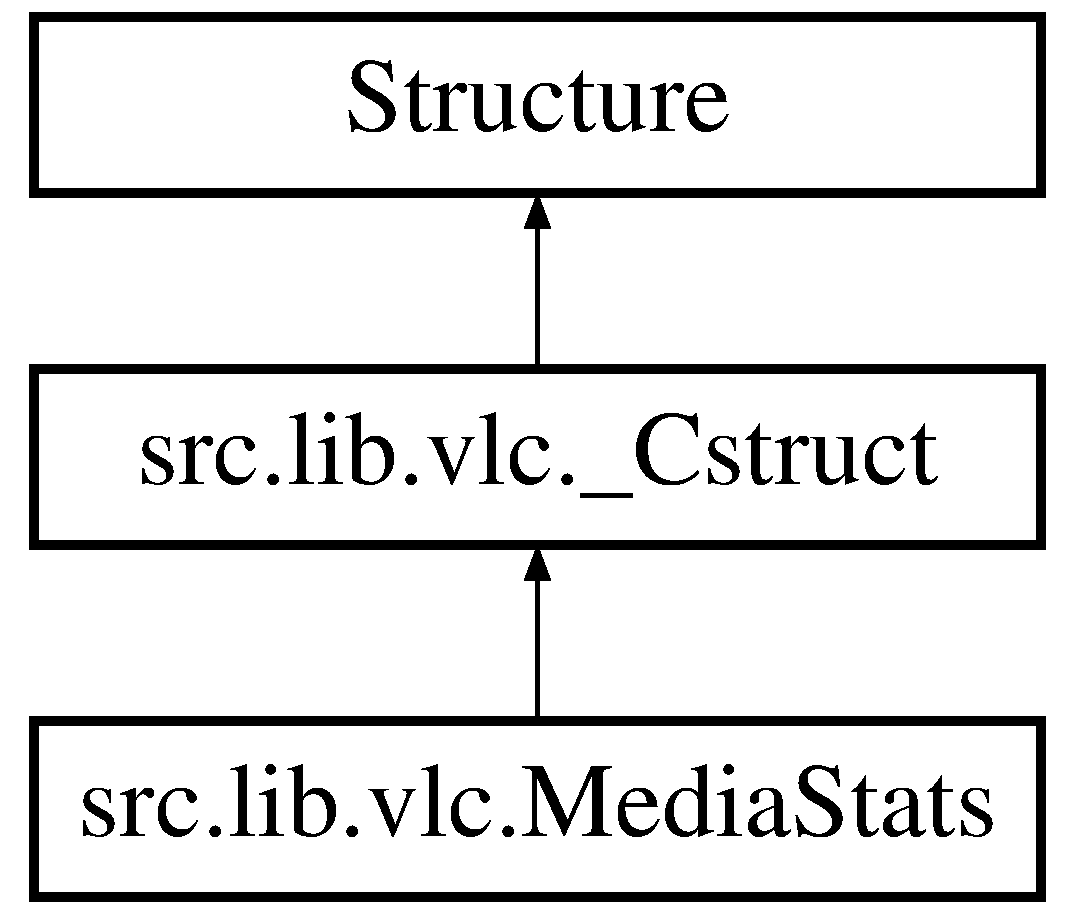
\includegraphics[height=3.000000cm]{classsrc_1_1lib_1_1vlc_1_1MediaStats}
\end{center}
\end{figure}
\subsection*{Static Private Attributes}
\begin{DoxyCompactItemize}
\item 
list \hyperlink{classsrc_1_1lib_1_1vlc_1_1MediaStats_a1f711ea68d94e8320bed627fd7be7b4d}{\+\_\+fields\+\_\+}
\end{DoxyCompactItemize}
\subsection*{Additional Inherited Members}


\subsection{Member Data Documentation}
\hypertarget{classsrc_1_1lib_1_1vlc_1_1MediaStats_a1f711ea68d94e8320bed627fd7be7b4d}{}\index{src\+::lib\+::vlc\+::\+Media\+Stats@{src\+::lib\+::vlc\+::\+Media\+Stats}!\+\_\+fields\+\_\+@{\+\_\+fields\+\_\+}}
\index{\+\_\+fields\+\_\+@{\+\_\+fields\+\_\+}!src\+::lib\+::vlc\+::\+Media\+Stats@{src\+::lib\+::vlc\+::\+Media\+Stats}}
\subsubsection[{\+\_\+fields\+\_\+}]{\setlength{\rightskip}{0pt plus 5cm}list src.\+lib.\+vlc.\+Media\+Stats.\+\_\+fields\+\_\+\hspace{0.3cm}{\ttfamily [static]}, {\ttfamily [private]}}\label{classsrc_1_1lib_1_1vlc_1_1MediaStats_a1f711ea68d94e8320bed627fd7be7b4d}
{\bfseries Initial value\+:}
\begin{DoxyCode}
1 = [
2         (\textcolor{stringliteral}{'read\_bytes'},          ctypes.c\_int  ),
3         (\textcolor{stringliteral}{'input\_bitrate'},       ctypes.c\_float),
4         (\textcolor{stringliteral}{'demux\_read\_bytes'},    ctypes.c\_int  ),
5         (\textcolor{stringliteral}{'demux\_bitrate'},       ctypes.c\_float),
6         (\textcolor{stringliteral}{'demux\_corrupted'},     ctypes.c\_int  ),
7         (\textcolor{stringliteral}{'demux\_discontinuity'}, ctypes.c\_int  ),
8         (\textcolor{stringliteral}{'decoded\_video'},       ctypes.c\_int  ),
9         (\textcolor{stringliteral}{'decoded\_audio'},       ctypes.c\_int  ),
10         (\textcolor{stringliteral}{'displayed\_pictures'},  ctypes.c\_int  ),
11         (\textcolor{stringliteral}{'lost\_pictures'},       ctypes.c\_int  ),
12         (\textcolor{stringliteral}{'played\_abuffers'},     ctypes.c\_int  ),
13         (\textcolor{stringliteral}{'lost\_abuffers'},       ctypes.c\_int  ),
14         (\textcolor{stringliteral}{'sent\_packets'},        ctypes.c\_int  ),
15         (\textcolor{stringliteral}{'sent\_bytes'},          ctypes.c\_int  ),
16         (\textcolor{stringliteral}{'send\_bitrate'},        ctypes.c\_float),
17     ]
\end{DoxyCode}


The documentation for this class was generated from the following file\+:\begin{DoxyCompactItemize}
\item 
src/lib/\hyperlink{vlc_8py}{vlc.\+py}\end{DoxyCompactItemize}

\hypertarget{classsrc_1_1lib_1_1vlc_1_1MediaTrackInfo}{}\section{src.\+lib.\+vlc.\+Media\+Track\+Info Class Reference}
\label{classsrc_1_1lib_1_1vlc_1_1MediaTrackInfo}\index{src.\+lib.\+vlc.\+Media\+Track\+Info@{src.\+lib.\+vlc.\+Media\+Track\+Info}}
Inheritance diagram for src.\+lib.\+vlc.\+Media\+Track\+Info\+:\begin{figure}[H]
\begin{center}
\leavevmode
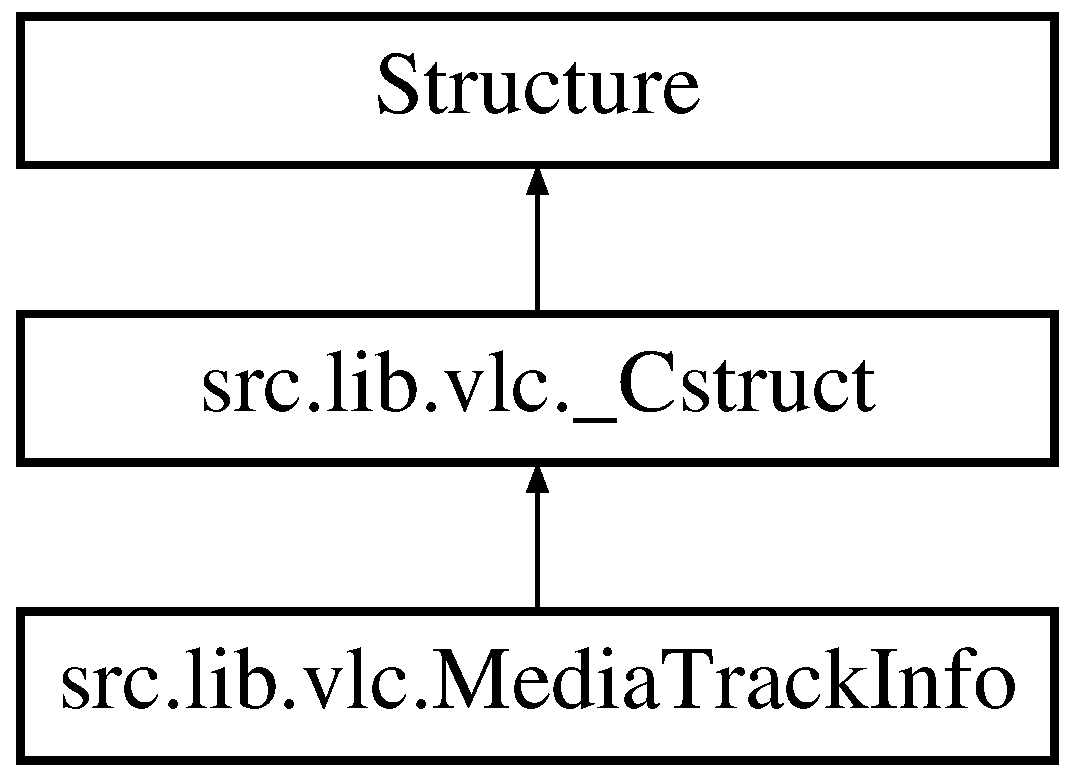
\includegraphics[height=3.000000cm]{classsrc_1_1lib_1_1vlc_1_1MediaTrackInfo}
\end{center}
\end{figure}
\subsection*{Static Private Attributes}
\begin{DoxyCompactItemize}
\item 
list \hyperlink{classsrc_1_1lib_1_1vlc_1_1MediaTrackInfo_a444f39463dae0df3bc71919b71f4afcd}{\+\_\+fields\+\_\+}
\end{DoxyCompactItemize}
\subsection*{Additional Inherited Members}


\subsection{Member Data Documentation}
\hypertarget{classsrc_1_1lib_1_1vlc_1_1MediaTrackInfo_a444f39463dae0df3bc71919b71f4afcd}{}\index{src\+::lib\+::vlc\+::\+Media\+Track\+Info@{src\+::lib\+::vlc\+::\+Media\+Track\+Info}!\+\_\+fields\+\_\+@{\+\_\+fields\+\_\+}}
\index{\+\_\+fields\+\_\+@{\+\_\+fields\+\_\+}!src\+::lib\+::vlc\+::\+Media\+Track\+Info@{src\+::lib\+::vlc\+::\+Media\+Track\+Info}}
\subsubsection[{\+\_\+fields\+\_\+}]{\setlength{\rightskip}{0pt plus 5cm}list src.\+lib.\+vlc.\+Media\+Track\+Info.\+\_\+fields\+\_\+\hspace{0.3cm}{\ttfamily [static]}, {\ttfamily [private]}}\label{classsrc_1_1lib_1_1vlc_1_1MediaTrackInfo_a444f39463dae0df3bc71919b71f4afcd}
{\bfseries Initial value\+:}
\begin{DoxyCode}
1 = [
2         (\textcolor{stringliteral}{'codec'},              ctypes.c\_uint32),
3         (\textcolor{stringliteral}{'id'},                 ctypes.c\_int   ),
4         (\textcolor{stringliteral}{'type'},               TrackType      ),
5         (\textcolor{stringliteral}{'profile'},            ctypes.c\_int   ),
6         (\textcolor{stringliteral}{'level'},              ctypes.c\_int   ),
7         (\textcolor{stringliteral}{'channels\_or\_height'}, ctypes.c\_uint  ),
8         (\textcolor{stringliteral}{'rate\_or\_width'},      ctypes.c\_uint  ),
9     ]
\end{DoxyCode}


The documentation for this class was generated from the following file\+:\begin{DoxyCompactItemize}
\item 
src/lib/\hyperlink{vlc_8py}{vlc.\+py}\end{DoxyCompactItemize}

\hypertarget{classsrc_1_1lib_1_1vlc_1_1Meta}{}\section{src.\+lib.\+vlc.\+Meta Class Reference}
\label{classsrc_1_1lib_1_1vlc_1_1Meta}\index{src.\+lib.\+vlc.\+Meta@{src.\+lib.\+vlc.\+Meta}}
Inheritance diagram for src.\+lib.\+vlc.\+Meta\+:\begin{figure}[H]
\begin{center}
\leavevmode
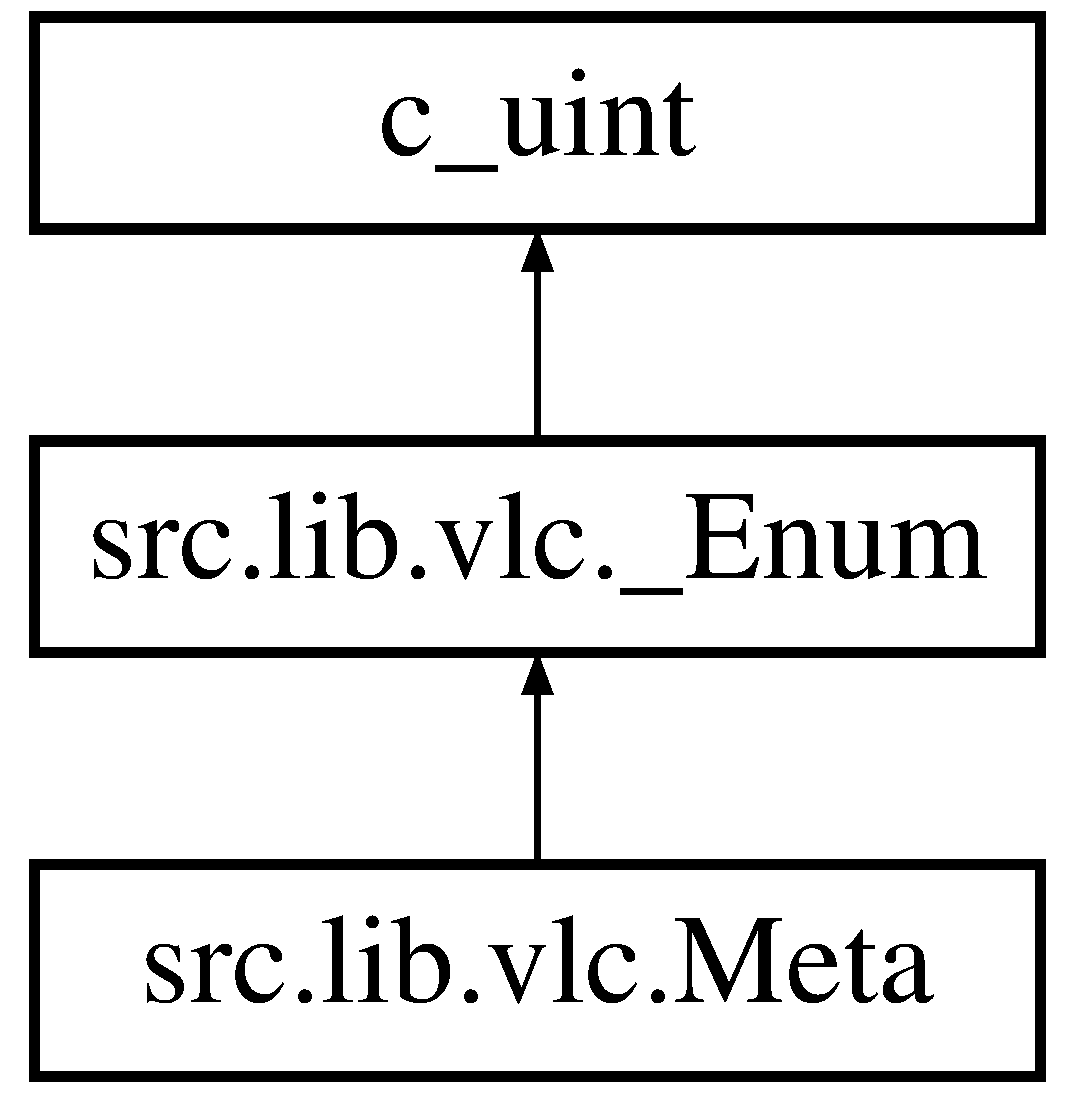
\includegraphics[height=3.000000cm]{classsrc_1_1lib_1_1vlc_1_1Meta}
\end{center}
\end{figure}
\subsection*{Static Private Attributes}
\begin{DoxyCompactItemize}
\item 
dictionary \hyperlink{classsrc_1_1lib_1_1vlc_1_1Meta_a9f7d14459cdacb3bd5c93b7f0c289a9b}{\+\_\+enum\+\_\+names\+\_\+}
\end{DoxyCompactItemize}
\subsection*{Additional Inherited Members}


\subsection{Detailed Description}
\begin{DoxyVerb}Meta data types.
\end{DoxyVerb}
 

\subsection{Member Data Documentation}
\hypertarget{classsrc_1_1lib_1_1vlc_1_1Meta_a9f7d14459cdacb3bd5c93b7f0c289a9b}{}\index{src\+::lib\+::vlc\+::\+Meta@{src\+::lib\+::vlc\+::\+Meta}!\+\_\+enum\+\_\+names\+\_\+@{\+\_\+enum\+\_\+names\+\_\+}}
\index{\+\_\+enum\+\_\+names\+\_\+@{\+\_\+enum\+\_\+names\+\_\+}!src\+::lib\+::vlc\+::\+Meta@{src\+::lib\+::vlc\+::\+Meta}}
\subsubsection[{\+\_\+enum\+\_\+names\+\_\+}]{\setlength{\rightskip}{0pt plus 5cm}dictionary src.\+lib.\+vlc.\+Meta.\+\_\+enum\+\_\+names\+\_\+\hspace{0.3cm}{\ttfamily [static]}, {\ttfamily [private]}}\label{classsrc_1_1lib_1_1vlc_1_1Meta_a9f7d14459cdacb3bd5c93b7f0c289a9b}
{\bfseries Initial value\+:}
\begin{DoxyCode}
1 = \{
2         0: \textcolor{stringliteral}{'Title'},
3         1: \textcolor{stringliteral}{'Artist'},
4         2: \textcolor{stringliteral}{'Genre'},
5         3: \textcolor{stringliteral}{'Copyright'},
6         4: \textcolor{stringliteral}{'Album'},
7         5: \textcolor{stringliteral}{'TrackNumber'},
8         6: \textcolor{stringliteral}{'Description'},
9         7: \textcolor{stringliteral}{'Rating'},
10         8: \textcolor{stringliteral}{'Date'},
11         9: \textcolor{stringliteral}{'Setting'},
12         10: \textcolor{stringliteral}{'URL'},
13         11: \textcolor{stringliteral}{'Language'},
14         12: \textcolor{stringliteral}{'NowPlaying'},
15         13: \textcolor{stringliteral}{'Publisher'},
16         14: \textcolor{stringliteral}{'EncodedBy'},
17         15: \textcolor{stringliteral}{'ArtworkURL'},
18         16: \textcolor{stringliteral}{'TrackID'},
19     \}
\end{DoxyCode}


The documentation for this class was generated from the following file\+:\begin{DoxyCompactItemize}
\item 
src/lib/\hyperlink{vlc_8py}{vlc.\+py}\end{DoxyCompactItemize}

\hypertarget{classsrc_1_1model_1_1model_1_1Model}{}\section{src.\+model.\+model.\+Model Class Reference}
\label{classsrc_1_1model_1_1model_1_1Model}\index{src.\+model.\+model.\+Model@{src.\+model.\+model.\+Model}}
\subsection*{Public Member Functions}
\begin{DoxyCompactItemize}
\item 
def \hyperlink{classsrc_1_1model_1_1model_1_1Model_a31bec154140cab88fb35302b083e707a}{\+\_\+\+\_\+init\+\_\+\+\_\+} (self)
\item 
def \hyperlink{classsrc_1_1model_1_1model_1_1Model_a1c9f885ffd733df328cdba66aebacceb}{get\+\_\+vlc\+\_\+player\+\_\+instance} (self)
\end{DoxyCompactItemize}
\subsection*{Public Attributes}
\begin{DoxyCompactItemize}
\item 
\hyperlink{classsrc_1_1model_1_1model_1_1Model_aa9deef378ecbbbaffcf4460afad320a7}{vlc\+\_\+player\+\_\+instance}
\end{DoxyCompactItemize}


\subsection{Constructor \& Destructor Documentation}
\hypertarget{classsrc_1_1model_1_1model_1_1Model_a31bec154140cab88fb35302b083e707a}{}\index{src\+::model\+::model\+::\+Model@{src\+::model\+::model\+::\+Model}!\+\_\+\+\_\+init\+\_\+\+\_\+@{\+\_\+\+\_\+init\+\_\+\+\_\+}}
\index{\+\_\+\+\_\+init\+\_\+\+\_\+@{\+\_\+\+\_\+init\+\_\+\+\_\+}!src\+::model\+::model\+::\+Model@{src\+::model\+::model\+::\+Model}}
\subsubsection[{\+\_\+\+\_\+init\+\_\+\+\_\+}]{\setlength{\rightskip}{0pt plus 5cm}def src.\+model.\+model.\+Model.\+\_\+\+\_\+init\+\_\+\+\_\+ (
\begin{DoxyParamCaption}
\item[{}]{self}
\end{DoxyParamCaption}
)}\label{classsrc_1_1model_1_1model_1_1Model_a31bec154140cab88fb35302b083e707a}


\subsection{Member Function Documentation}
\hypertarget{classsrc_1_1model_1_1model_1_1Model_a1c9f885ffd733df328cdba66aebacceb}{}\index{src\+::model\+::model\+::\+Model@{src\+::model\+::model\+::\+Model}!get\+\_\+vlc\+\_\+player\+\_\+instance@{get\+\_\+vlc\+\_\+player\+\_\+instance}}
\index{get\+\_\+vlc\+\_\+player\+\_\+instance@{get\+\_\+vlc\+\_\+player\+\_\+instance}!src\+::model\+::model\+::\+Model@{src\+::model\+::model\+::\+Model}}
\subsubsection[{get\+\_\+vlc\+\_\+player\+\_\+instance}]{\setlength{\rightskip}{0pt plus 5cm}def src.\+model.\+model.\+Model.\+get\+\_\+vlc\+\_\+player\+\_\+instance (
\begin{DoxyParamCaption}
\item[{}]{self}
\end{DoxyParamCaption}
)}\label{classsrc_1_1model_1_1model_1_1Model_a1c9f885ffd733df328cdba66aebacceb}


\subsection{Member Data Documentation}
\hypertarget{classsrc_1_1model_1_1model_1_1Model_aa9deef378ecbbbaffcf4460afad320a7}{}\index{src\+::model\+::model\+::\+Model@{src\+::model\+::model\+::\+Model}!vlc\+\_\+player\+\_\+instance@{vlc\+\_\+player\+\_\+instance}}
\index{vlc\+\_\+player\+\_\+instance@{vlc\+\_\+player\+\_\+instance}!src\+::model\+::model\+::\+Model@{src\+::model\+::model\+::\+Model}}
\subsubsection[{vlc\+\_\+player\+\_\+instance}]{\setlength{\rightskip}{0pt plus 5cm}src.\+model.\+model.\+Model.\+vlc\+\_\+player\+\_\+instance}\label{classsrc_1_1model_1_1model_1_1Model_aa9deef378ecbbbaffcf4460afad320a7}


The documentation for this class was generated from the following file\+:\begin{DoxyCompactItemize}
\item 
src/model/\hyperlink{model_8py}{model.\+py}\end{DoxyCompactItemize}

\hypertarget{classsrc_1_1lib_1_1vlc_1_1ModuleDescription}{}\section{src.\+lib.\+vlc.\+Module\+Description Class Reference}
\label{classsrc_1_1lib_1_1vlc_1_1ModuleDescription}\index{src.\+lib.\+vlc.\+Module\+Description@{src.\+lib.\+vlc.\+Module\+Description}}
Inheritance diagram for src.\+lib.\+vlc.\+Module\+Description\+:\begin{figure}[H]
\begin{center}
\leavevmode
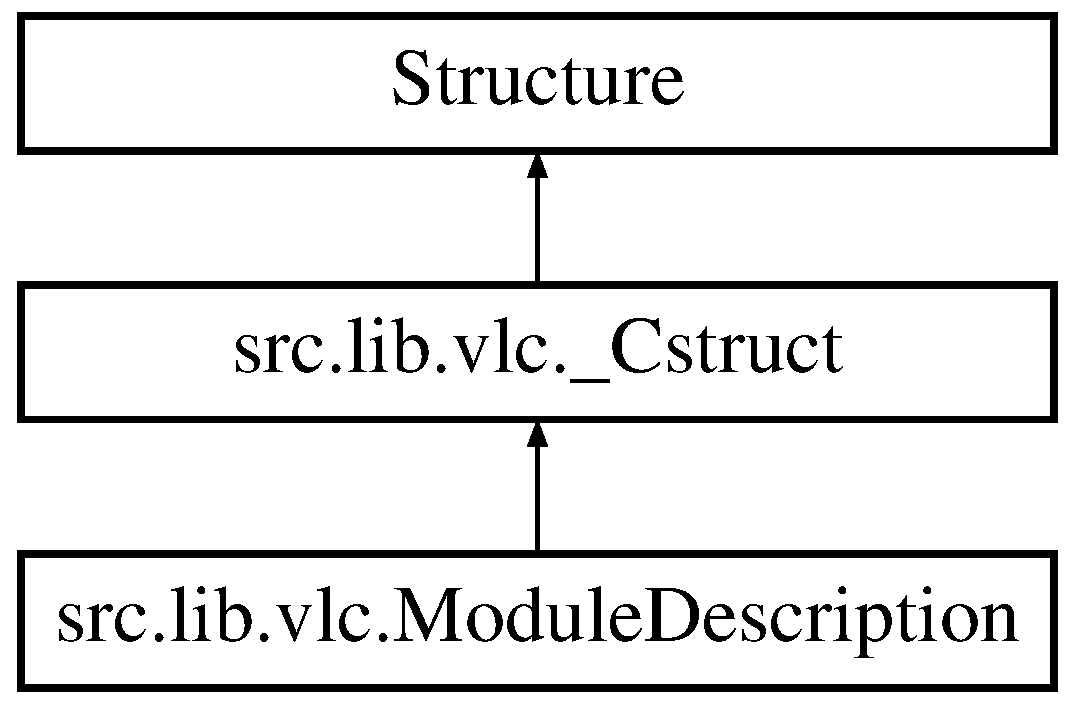
\includegraphics[height=3.000000cm]{classsrc_1_1lib_1_1vlc_1_1ModuleDescription}
\end{center}
\end{figure}
\subsection*{Public Member Functions}
\begin{DoxyCompactItemize}
\item 
def \hyperlink{classsrc_1_1lib_1_1vlc_1_1ModuleDescription_ad3d0e58809d8946ba2097b99af3007d4}{\+\_\+\+\_\+str\+\_\+\+\_\+} (self)
\end{DoxyCompactItemize}


\subsection{Member Function Documentation}
\hypertarget{classsrc_1_1lib_1_1vlc_1_1ModuleDescription_ad3d0e58809d8946ba2097b99af3007d4}{}\index{src\+::lib\+::vlc\+::\+Module\+Description@{src\+::lib\+::vlc\+::\+Module\+Description}!\+\_\+\+\_\+str\+\_\+\+\_\+@{\+\_\+\+\_\+str\+\_\+\+\_\+}}
\index{\+\_\+\+\_\+str\+\_\+\+\_\+@{\+\_\+\+\_\+str\+\_\+\+\_\+}!src\+::lib\+::vlc\+::\+Module\+Description@{src\+::lib\+::vlc\+::\+Module\+Description}}
\subsubsection[{\+\_\+\+\_\+str\+\_\+\+\_\+}]{\setlength{\rightskip}{0pt plus 5cm}def src.\+lib.\+vlc.\+Module\+Description.\+\_\+\+\_\+str\+\_\+\+\_\+ (
\begin{DoxyParamCaption}
\item[{}]{self}
\end{DoxyParamCaption}
)}\label{classsrc_1_1lib_1_1vlc_1_1ModuleDescription_ad3d0e58809d8946ba2097b99af3007d4}


The documentation for this class was generated from the following file\+:\begin{DoxyCompactItemize}
\item 
src/lib/\hyperlink{vlc_8py}{vlc.\+py}\end{DoxyCompactItemize}

\hypertarget{classsrc_1_1core_1_1monitor__dbs_1_1Monitor__DBS}{}\section{src.\+core.\+monitor\+\_\+dbs.\+Monitor\+\_\+\+D\+B\+S Class Reference}
\label{classsrc_1_1core_1_1monitor__dbs_1_1Monitor__DBS}\index{src.\+core.\+monitor\+\_\+dbs.\+Monitor\+\_\+\+D\+B\+S@{src.\+core.\+monitor\+\_\+dbs.\+Monitor\+\_\+\+D\+B\+S}}
Inheritance diagram for src.\+core.\+monitor\+\_\+dbs.\+Monitor\+\_\+\+D\+B\+S\+:\begin{figure}[H]
\begin{center}
\leavevmode
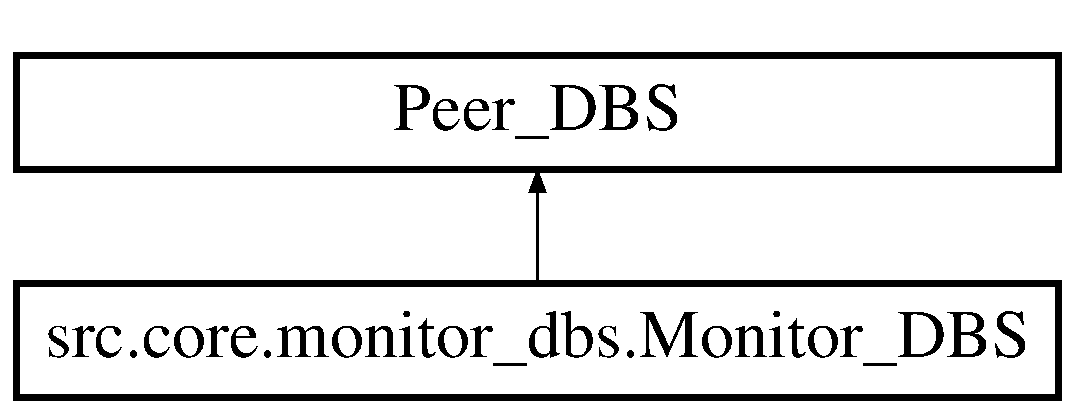
\includegraphics[height=2.000000cm]{classsrc_1_1core_1_1monitor__dbs_1_1Monitor__DBS}
\end{center}
\end{figure}
\subsection*{Public Member Functions}
\begin{DoxyCompactItemize}
\item 
def \hyperlink{classsrc_1_1core_1_1monitor__dbs_1_1Monitor__DBS_a3897dc219b9cc6debd5e594fb2c4868e}{\+\_\+\+\_\+init\+\_\+\+\_\+} (self, peer)
\item 
def \hyperlink{classsrc_1_1core_1_1monitor__dbs_1_1Monitor__DBS_a5555b20bb26c70d2dfd74783c6a8f1c0}{print\+\_\+the\+\_\+module\+\_\+name} (self)
\item 
def \hyperlink{classsrc_1_1core_1_1monitor__dbs_1_1Monitor__DBS_a0d826b0dd76eae682d79c4b4939fe724}{complain} (self, chunk\+\_\+number)
\item 
def \hyperlink{classsrc_1_1core_1_1monitor__dbs_1_1Monitor__DBS_a7f2825bf8b6743ebee9fc61eb8a5ba91}{find\+\_\+next\+\_\+chunk} (self)
\end{DoxyCompactItemize}
\subsection*{Public Attributes}
\begin{DoxyCompactItemize}
\item 
\hyperlink{classsrc_1_1core_1_1monitor__dbs_1_1Monitor__DBS_ad37e37d4d9783c5f5b348ec489089c8a}{peer\+\_\+list}
\item 
\hyperlink{classsrc_1_1core_1_1monitor__dbs_1_1Monitor__DBS_af81d83715205435bac9b104f55fe1156}{splitter\+\_\+socket}
\item 
\hyperlink{classsrc_1_1core_1_1monitor__dbs_1_1Monitor__DBS_a8b7ada3a3f74f3b21d3566db9e9fd62f}{buffer\+\_\+size}
\item 
\hyperlink{classsrc_1_1core_1_1monitor__dbs_1_1Monitor__DBS_a4a80ef01a9b32917f1786b3637fa232a}{splitter}
\item 
\hyperlink{classsrc_1_1core_1_1monitor__dbs_1_1Monitor__DBS_acf320a0bf563ae5a480fd810c5ec45ff}{debt}
\item 
\hyperlink{classsrc_1_1core_1_1monitor__dbs_1_1Monitor__DBS_aec49095dbaeb66af772260dafe10d52e}{chunk\+\_\+size}
\item 
\hyperlink{classsrc_1_1core_1_1monitor__dbs_1_1Monitor__DBS_a4eb88bd5737b02b0520172ead3a623c2}{player\+\_\+socket}
\item 
\hyperlink{classsrc_1_1core_1_1monitor__dbs_1_1Monitor__DBS_af1a0c7877a6a78f36373a8184bd43775}{message\+\_\+format}
\item 
\hyperlink{classsrc_1_1core_1_1monitor__dbs_1_1Monitor__DBS_aae3ea0974cb300f573270131c1ec35b0}{team\+\_\+socket}
\end{DoxyCompactItemize}


\subsection{Constructor \& Destructor Documentation}
\hypertarget{classsrc_1_1core_1_1monitor__dbs_1_1Monitor__DBS_a3897dc219b9cc6debd5e594fb2c4868e}{}\index{src\+::core\+::monitor\+\_\+dbs\+::\+Monitor\+\_\+\+D\+B\+S@{src\+::core\+::monitor\+\_\+dbs\+::\+Monitor\+\_\+\+D\+B\+S}!\+\_\+\+\_\+init\+\_\+\+\_\+@{\+\_\+\+\_\+init\+\_\+\+\_\+}}
\index{\+\_\+\+\_\+init\+\_\+\+\_\+@{\+\_\+\+\_\+init\+\_\+\+\_\+}!src\+::core\+::monitor\+\_\+dbs\+::\+Monitor\+\_\+\+D\+B\+S@{src\+::core\+::monitor\+\_\+dbs\+::\+Monitor\+\_\+\+D\+B\+S}}
\subsubsection[{\+\_\+\+\_\+init\+\_\+\+\_\+}]{\setlength{\rightskip}{0pt plus 5cm}def src.\+core.\+monitor\+\_\+dbs.\+Monitor\+\_\+\+D\+B\+S.\+\_\+\+\_\+init\+\_\+\+\_\+ (
\begin{DoxyParamCaption}
\item[{}]{self, }
\item[{}]{peer}
\end{DoxyParamCaption}
)}\label{classsrc_1_1core_1_1monitor__dbs_1_1Monitor__DBS_a3897dc219b9cc6debd5e594fb2c4868e}


\subsection{Member Function Documentation}
\hypertarget{classsrc_1_1core_1_1monitor__dbs_1_1Monitor__DBS_a0d826b0dd76eae682d79c4b4939fe724}{}\index{src\+::core\+::monitor\+\_\+dbs\+::\+Monitor\+\_\+\+D\+B\+S@{src\+::core\+::monitor\+\_\+dbs\+::\+Monitor\+\_\+\+D\+B\+S}!complain@{complain}}
\index{complain@{complain}!src\+::core\+::monitor\+\_\+dbs\+::\+Monitor\+\_\+\+D\+B\+S@{src\+::core\+::monitor\+\_\+dbs\+::\+Monitor\+\_\+\+D\+B\+S}}
\subsubsection[{complain}]{\setlength{\rightskip}{0pt plus 5cm}def src.\+core.\+monitor\+\_\+dbs.\+Monitor\+\_\+\+D\+B\+S.\+complain (
\begin{DoxyParamCaption}
\item[{}]{self, }
\item[{}]{chunk\+\_\+number}
\end{DoxyParamCaption}
)}\label{classsrc_1_1core_1_1monitor__dbs_1_1Monitor__DBS_a0d826b0dd76eae682d79c4b4939fe724}
\hypertarget{classsrc_1_1core_1_1monitor__dbs_1_1Monitor__DBS_a7f2825bf8b6743ebee9fc61eb8a5ba91}{}\index{src\+::core\+::monitor\+\_\+dbs\+::\+Monitor\+\_\+\+D\+B\+S@{src\+::core\+::monitor\+\_\+dbs\+::\+Monitor\+\_\+\+D\+B\+S}!find\+\_\+next\+\_\+chunk@{find\+\_\+next\+\_\+chunk}}
\index{find\+\_\+next\+\_\+chunk@{find\+\_\+next\+\_\+chunk}!src\+::core\+::monitor\+\_\+dbs\+::\+Monitor\+\_\+\+D\+B\+S@{src\+::core\+::monitor\+\_\+dbs\+::\+Monitor\+\_\+\+D\+B\+S}}
\subsubsection[{find\+\_\+next\+\_\+chunk}]{\setlength{\rightskip}{0pt plus 5cm}def src.\+core.\+monitor\+\_\+dbs.\+Monitor\+\_\+\+D\+B\+S.\+find\+\_\+next\+\_\+chunk (
\begin{DoxyParamCaption}
\item[{}]{self}
\end{DoxyParamCaption}
)}\label{classsrc_1_1core_1_1monitor__dbs_1_1Monitor__DBS_a7f2825bf8b6743ebee9fc61eb8a5ba91}
\hypertarget{classsrc_1_1core_1_1monitor__dbs_1_1Monitor__DBS_a5555b20bb26c70d2dfd74783c6a8f1c0}{}\index{src\+::core\+::monitor\+\_\+dbs\+::\+Monitor\+\_\+\+D\+B\+S@{src\+::core\+::monitor\+\_\+dbs\+::\+Monitor\+\_\+\+D\+B\+S}!print\+\_\+the\+\_\+module\+\_\+name@{print\+\_\+the\+\_\+module\+\_\+name}}
\index{print\+\_\+the\+\_\+module\+\_\+name@{print\+\_\+the\+\_\+module\+\_\+name}!src\+::core\+::monitor\+\_\+dbs\+::\+Monitor\+\_\+\+D\+B\+S@{src\+::core\+::monitor\+\_\+dbs\+::\+Monitor\+\_\+\+D\+B\+S}}
\subsubsection[{print\+\_\+the\+\_\+module\+\_\+name}]{\setlength{\rightskip}{0pt plus 5cm}def src.\+core.\+monitor\+\_\+dbs.\+Monitor\+\_\+\+D\+B\+S.\+print\+\_\+the\+\_\+module\+\_\+name (
\begin{DoxyParamCaption}
\item[{}]{self}
\end{DoxyParamCaption}
)}\label{classsrc_1_1core_1_1monitor__dbs_1_1Monitor__DBS_a5555b20bb26c70d2dfd74783c6a8f1c0}


\subsection{Member Data Documentation}
\hypertarget{classsrc_1_1core_1_1monitor__dbs_1_1Monitor__DBS_a8b7ada3a3f74f3b21d3566db9e9fd62f}{}\index{src\+::core\+::monitor\+\_\+dbs\+::\+Monitor\+\_\+\+D\+B\+S@{src\+::core\+::monitor\+\_\+dbs\+::\+Monitor\+\_\+\+D\+B\+S}!buffer\+\_\+size@{buffer\+\_\+size}}
\index{buffer\+\_\+size@{buffer\+\_\+size}!src\+::core\+::monitor\+\_\+dbs\+::\+Monitor\+\_\+\+D\+B\+S@{src\+::core\+::monitor\+\_\+dbs\+::\+Monitor\+\_\+\+D\+B\+S}}
\subsubsection[{buffer\+\_\+size}]{\setlength{\rightskip}{0pt plus 5cm}src.\+core.\+monitor\+\_\+dbs.\+Monitor\+\_\+\+D\+B\+S.\+buffer\+\_\+size}\label{classsrc_1_1core_1_1monitor__dbs_1_1Monitor__DBS_a8b7ada3a3f74f3b21d3566db9e9fd62f}
\hypertarget{classsrc_1_1core_1_1monitor__dbs_1_1Monitor__DBS_aec49095dbaeb66af772260dafe10d52e}{}\index{src\+::core\+::monitor\+\_\+dbs\+::\+Monitor\+\_\+\+D\+B\+S@{src\+::core\+::monitor\+\_\+dbs\+::\+Monitor\+\_\+\+D\+B\+S}!chunk\+\_\+size@{chunk\+\_\+size}}
\index{chunk\+\_\+size@{chunk\+\_\+size}!src\+::core\+::monitor\+\_\+dbs\+::\+Monitor\+\_\+\+D\+B\+S@{src\+::core\+::monitor\+\_\+dbs\+::\+Monitor\+\_\+\+D\+B\+S}}
\subsubsection[{chunk\+\_\+size}]{\setlength{\rightskip}{0pt plus 5cm}src.\+core.\+monitor\+\_\+dbs.\+Monitor\+\_\+\+D\+B\+S.\+chunk\+\_\+size}\label{classsrc_1_1core_1_1monitor__dbs_1_1Monitor__DBS_aec49095dbaeb66af772260dafe10d52e}
\hypertarget{classsrc_1_1core_1_1monitor__dbs_1_1Monitor__DBS_acf320a0bf563ae5a480fd810c5ec45ff}{}\index{src\+::core\+::monitor\+\_\+dbs\+::\+Monitor\+\_\+\+D\+B\+S@{src\+::core\+::monitor\+\_\+dbs\+::\+Monitor\+\_\+\+D\+B\+S}!debt@{debt}}
\index{debt@{debt}!src\+::core\+::monitor\+\_\+dbs\+::\+Monitor\+\_\+\+D\+B\+S@{src\+::core\+::monitor\+\_\+dbs\+::\+Monitor\+\_\+\+D\+B\+S}}
\subsubsection[{debt}]{\setlength{\rightskip}{0pt plus 5cm}src.\+core.\+monitor\+\_\+dbs.\+Monitor\+\_\+\+D\+B\+S.\+debt}\label{classsrc_1_1core_1_1monitor__dbs_1_1Monitor__DBS_acf320a0bf563ae5a480fd810c5ec45ff}
\hypertarget{classsrc_1_1core_1_1monitor__dbs_1_1Monitor__DBS_af1a0c7877a6a78f36373a8184bd43775}{}\index{src\+::core\+::monitor\+\_\+dbs\+::\+Monitor\+\_\+\+D\+B\+S@{src\+::core\+::monitor\+\_\+dbs\+::\+Monitor\+\_\+\+D\+B\+S}!message\+\_\+format@{message\+\_\+format}}
\index{message\+\_\+format@{message\+\_\+format}!src\+::core\+::monitor\+\_\+dbs\+::\+Monitor\+\_\+\+D\+B\+S@{src\+::core\+::monitor\+\_\+dbs\+::\+Monitor\+\_\+\+D\+B\+S}}
\subsubsection[{message\+\_\+format}]{\setlength{\rightskip}{0pt plus 5cm}src.\+core.\+monitor\+\_\+dbs.\+Monitor\+\_\+\+D\+B\+S.\+message\+\_\+format}\label{classsrc_1_1core_1_1monitor__dbs_1_1Monitor__DBS_af1a0c7877a6a78f36373a8184bd43775}
\hypertarget{classsrc_1_1core_1_1monitor__dbs_1_1Monitor__DBS_ad37e37d4d9783c5f5b348ec489089c8a}{}\index{src\+::core\+::monitor\+\_\+dbs\+::\+Monitor\+\_\+\+D\+B\+S@{src\+::core\+::monitor\+\_\+dbs\+::\+Monitor\+\_\+\+D\+B\+S}!peer\+\_\+list@{peer\+\_\+list}}
\index{peer\+\_\+list@{peer\+\_\+list}!src\+::core\+::monitor\+\_\+dbs\+::\+Monitor\+\_\+\+D\+B\+S@{src\+::core\+::monitor\+\_\+dbs\+::\+Monitor\+\_\+\+D\+B\+S}}
\subsubsection[{peer\+\_\+list}]{\setlength{\rightskip}{0pt plus 5cm}src.\+core.\+monitor\+\_\+dbs.\+Monitor\+\_\+\+D\+B\+S.\+peer\+\_\+list}\label{classsrc_1_1core_1_1monitor__dbs_1_1Monitor__DBS_ad37e37d4d9783c5f5b348ec489089c8a}
\hypertarget{classsrc_1_1core_1_1monitor__dbs_1_1Monitor__DBS_a4eb88bd5737b02b0520172ead3a623c2}{}\index{src\+::core\+::monitor\+\_\+dbs\+::\+Monitor\+\_\+\+D\+B\+S@{src\+::core\+::monitor\+\_\+dbs\+::\+Monitor\+\_\+\+D\+B\+S}!player\+\_\+socket@{player\+\_\+socket}}
\index{player\+\_\+socket@{player\+\_\+socket}!src\+::core\+::monitor\+\_\+dbs\+::\+Monitor\+\_\+\+D\+B\+S@{src\+::core\+::monitor\+\_\+dbs\+::\+Monitor\+\_\+\+D\+B\+S}}
\subsubsection[{player\+\_\+socket}]{\setlength{\rightskip}{0pt plus 5cm}src.\+core.\+monitor\+\_\+dbs.\+Monitor\+\_\+\+D\+B\+S.\+player\+\_\+socket}\label{classsrc_1_1core_1_1monitor__dbs_1_1Monitor__DBS_a4eb88bd5737b02b0520172ead3a623c2}
\hypertarget{classsrc_1_1core_1_1monitor__dbs_1_1Monitor__DBS_a4a80ef01a9b32917f1786b3637fa232a}{}\index{src\+::core\+::monitor\+\_\+dbs\+::\+Monitor\+\_\+\+D\+B\+S@{src\+::core\+::monitor\+\_\+dbs\+::\+Monitor\+\_\+\+D\+B\+S}!splitter@{splitter}}
\index{splitter@{splitter}!src\+::core\+::monitor\+\_\+dbs\+::\+Monitor\+\_\+\+D\+B\+S@{src\+::core\+::monitor\+\_\+dbs\+::\+Monitor\+\_\+\+D\+B\+S}}
\subsubsection[{splitter}]{\setlength{\rightskip}{0pt plus 5cm}src.\+core.\+monitor\+\_\+dbs.\+Monitor\+\_\+\+D\+B\+S.\+splitter}\label{classsrc_1_1core_1_1monitor__dbs_1_1Monitor__DBS_a4a80ef01a9b32917f1786b3637fa232a}
\hypertarget{classsrc_1_1core_1_1monitor__dbs_1_1Monitor__DBS_af81d83715205435bac9b104f55fe1156}{}\index{src\+::core\+::monitor\+\_\+dbs\+::\+Monitor\+\_\+\+D\+B\+S@{src\+::core\+::monitor\+\_\+dbs\+::\+Monitor\+\_\+\+D\+B\+S}!splitter\+\_\+socket@{splitter\+\_\+socket}}
\index{splitter\+\_\+socket@{splitter\+\_\+socket}!src\+::core\+::monitor\+\_\+dbs\+::\+Monitor\+\_\+\+D\+B\+S@{src\+::core\+::monitor\+\_\+dbs\+::\+Monitor\+\_\+\+D\+B\+S}}
\subsubsection[{splitter\+\_\+socket}]{\setlength{\rightskip}{0pt plus 5cm}src.\+core.\+monitor\+\_\+dbs.\+Monitor\+\_\+\+D\+B\+S.\+splitter\+\_\+socket}\label{classsrc_1_1core_1_1monitor__dbs_1_1Monitor__DBS_af81d83715205435bac9b104f55fe1156}
\hypertarget{classsrc_1_1core_1_1monitor__dbs_1_1Monitor__DBS_aae3ea0974cb300f573270131c1ec35b0}{}\index{src\+::core\+::monitor\+\_\+dbs\+::\+Monitor\+\_\+\+D\+B\+S@{src\+::core\+::monitor\+\_\+dbs\+::\+Monitor\+\_\+\+D\+B\+S}!team\+\_\+socket@{team\+\_\+socket}}
\index{team\+\_\+socket@{team\+\_\+socket}!src\+::core\+::monitor\+\_\+dbs\+::\+Monitor\+\_\+\+D\+B\+S@{src\+::core\+::monitor\+\_\+dbs\+::\+Monitor\+\_\+\+D\+B\+S}}
\subsubsection[{team\+\_\+socket}]{\setlength{\rightskip}{0pt plus 5cm}src.\+core.\+monitor\+\_\+dbs.\+Monitor\+\_\+\+D\+B\+S.\+team\+\_\+socket}\label{classsrc_1_1core_1_1monitor__dbs_1_1Monitor__DBS_aae3ea0974cb300f573270131c1ec35b0}


The documentation for this class was generated from the following file\+:\begin{DoxyCompactItemize}
\item 
src/core/\hyperlink{monitor__dbs_8py}{monitor\+\_\+dbs.\+py}\end{DoxyCompactItemize}

\hypertarget{classsrc_1_1core_1_1monitor__fns_1_1Monitor__FNS}{}\section{src.\+core.\+monitor\+\_\+fns.\+Monitor\+\_\+\+F\+N\+S Class Reference}
\label{classsrc_1_1core_1_1monitor__fns_1_1Monitor__FNS}\index{src.\+core.\+monitor\+\_\+fns.\+Monitor\+\_\+\+F\+N\+S@{src.\+core.\+monitor\+\_\+fns.\+Monitor\+\_\+\+F\+N\+S}}
Inheritance diagram for src.\+core.\+monitor\+\_\+fns.\+Monitor\+\_\+\+F\+N\+S\+:\begin{figure}[H]
\begin{center}
\leavevmode
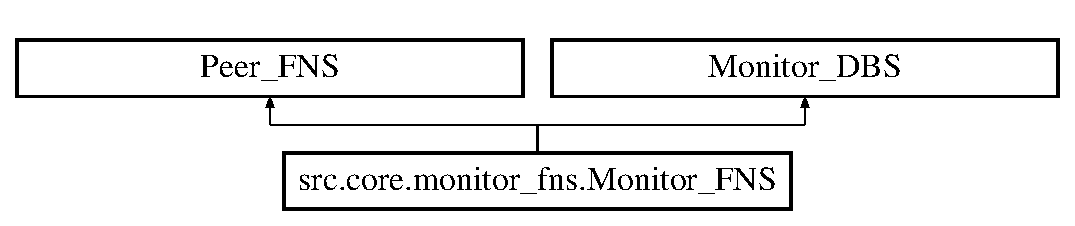
\includegraphics[height=2.000000cm]{classsrc_1_1core_1_1monitor__fns_1_1Monitor__FNS}
\end{center}
\end{figure}
\subsection*{Public Member Functions}
\begin{DoxyCompactItemize}
\item 
def \hyperlink{classsrc_1_1core_1_1monitor__fns_1_1Monitor__FNS_a8ef57d6be91a904455b027b81a0fa6d1}{\+\_\+\+\_\+init\+\_\+\+\_\+} (self, peer)
\item 
def \hyperlink{classsrc_1_1core_1_1monitor__fns_1_1Monitor__FNS_af3d7aea010da0326593d61763337d8b8}{say\+\_\+hello} (self, node)
\item 
def \hyperlink{classsrc_1_1core_1_1monitor__fns_1_1Monitor__FNS_acbbb9c80f3d7224f07d08aac5e06a0ea}{say\+\_\+goodbye} (self, node)
\item 
def \hyperlink{classsrc_1_1core_1_1monitor__fns_1_1Monitor__FNS_a5147f0b68fcf31d81f2c6ec2d5cb7eb3}{disconnect\+\_\+from\+\_\+the\+\_\+splitter} (self)
\end{DoxyCompactItemize}
\subsection*{Public Attributes}
\begin{DoxyCompactItemize}
\item 
\hyperlink{classsrc_1_1core_1_1monitor__fns_1_1Monitor__FNS_ade5cbdf60c6d114196aac3b792cbc4bc}{splitter\+\_\+socket}
\item 
\hyperlink{classsrc_1_1core_1_1monitor__fns_1_1Monitor__FNS_ab9a673dee77e79a32da5ee8f8835628f}{player\+\_\+socket}
\item 
\hyperlink{classsrc_1_1core_1_1monitor__fns_1_1Monitor__FNS_a90add17020e7b17140ca5eb479835f64}{buffer\+\_\+size}
\item 
\hyperlink{classsrc_1_1core_1_1monitor__fns_1_1Monitor__FNS_afc8566d86fed38cc81f634809fbab1e3}{chunk\+\_\+format\+\_\+string}
\item 
\hyperlink{classsrc_1_1core_1_1monitor__fns_1_1Monitor__FNS_abf30927507278ff68690466cae9379e9}{splitter}
\item 
\hyperlink{classsrc_1_1core_1_1monitor__fns_1_1Monitor__FNS_a7b9f5dd741c5c20b2d43b2d6117b2f62}{chunk\+\_\+size}
\item 
\hyperlink{classsrc_1_1core_1_1monitor__fns_1_1Monitor__FNS_a196bfd78037271343f39797f029f3230}{peer\+\_\+list}
\item 
\hyperlink{classsrc_1_1core_1_1monitor__fns_1_1Monitor__FNS_a01f110e1066e97cebdf5b28df0bd7c6c}{debt}
\end{DoxyCompactItemize}


\subsection{Constructor \& Destructor Documentation}
\hypertarget{classsrc_1_1core_1_1monitor__fns_1_1Monitor__FNS_a8ef57d6be91a904455b027b81a0fa6d1}{}\index{src\+::core\+::monitor\+\_\+fns\+::\+Monitor\+\_\+\+F\+N\+S@{src\+::core\+::monitor\+\_\+fns\+::\+Monitor\+\_\+\+F\+N\+S}!\+\_\+\+\_\+init\+\_\+\+\_\+@{\+\_\+\+\_\+init\+\_\+\+\_\+}}
\index{\+\_\+\+\_\+init\+\_\+\+\_\+@{\+\_\+\+\_\+init\+\_\+\+\_\+}!src\+::core\+::monitor\+\_\+fns\+::\+Monitor\+\_\+\+F\+N\+S@{src\+::core\+::monitor\+\_\+fns\+::\+Monitor\+\_\+\+F\+N\+S}}
\subsubsection[{\+\_\+\+\_\+init\+\_\+\+\_\+}]{\setlength{\rightskip}{0pt plus 5cm}def src.\+core.\+monitor\+\_\+fns.\+Monitor\+\_\+\+F\+N\+S.\+\_\+\+\_\+init\+\_\+\+\_\+ (
\begin{DoxyParamCaption}
\item[{}]{self, }
\item[{}]{peer}
\end{DoxyParamCaption}
)}\label{classsrc_1_1core_1_1monitor__fns_1_1Monitor__FNS_a8ef57d6be91a904455b027b81a0fa6d1}


\subsection{Member Function Documentation}
\hypertarget{classsrc_1_1core_1_1monitor__fns_1_1Monitor__FNS_a5147f0b68fcf31d81f2c6ec2d5cb7eb3}{}\index{src\+::core\+::monitor\+\_\+fns\+::\+Monitor\+\_\+\+F\+N\+S@{src\+::core\+::monitor\+\_\+fns\+::\+Monitor\+\_\+\+F\+N\+S}!disconnect\+\_\+from\+\_\+the\+\_\+splitter@{disconnect\+\_\+from\+\_\+the\+\_\+splitter}}
\index{disconnect\+\_\+from\+\_\+the\+\_\+splitter@{disconnect\+\_\+from\+\_\+the\+\_\+splitter}!src\+::core\+::monitor\+\_\+fns\+::\+Monitor\+\_\+\+F\+N\+S@{src\+::core\+::monitor\+\_\+fns\+::\+Monitor\+\_\+\+F\+N\+S}}
\subsubsection[{disconnect\+\_\+from\+\_\+the\+\_\+splitter}]{\setlength{\rightskip}{0pt plus 5cm}def src.\+core.\+monitor\+\_\+fns.\+Monitor\+\_\+\+F\+N\+S.\+disconnect\+\_\+from\+\_\+the\+\_\+splitter (
\begin{DoxyParamCaption}
\item[{}]{self}
\end{DoxyParamCaption}
)}\label{classsrc_1_1core_1_1monitor__fns_1_1Monitor__FNS_a5147f0b68fcf31d81f2c6ec2d5cb7eb3}
\hypertarget{classsrc_1_1core_1_1monitor__fns_1_1Monitor__FNS_acbbb9c80f3d7224f07d08aac5e06a0ea}{}\index{src\+::core\+::monitor\+\_\+fns\+::\+Monitor\+\_\+\+F\+N\+S@{src\+::core\+::monitor\+\_\+fns\+::\+Monitor\+\_\+\+F\+N\+S}!say\+\_\+goodbye@{say\+\_\+goodbye}}
\index{say\+\_\+goodbye@{say\+\_\+goodbye}!src\+::core\+::monitor\+\_\+fns\+::\+Monitor\+\_\+\+F\+N\+S@{src\+::core\+::monitor\+\_\+fns\+::\+Monitor\+\_\+\+F\+N\+S}}
\subsubsection[{say\+\_\+goodbye}]{\setlength{\rightskip}{0pt plus 5cm}def src.\+core.\+monitor\+\_\+fns.\+Monitor\+\_\+\+F\+N\+S.\+say\+\_\+goodbye (
\begin{DoxyParamCaption}
\item[{}]{self, }
\item[{}]{node}
\end{DoxyParamCaption}
)}\label{classsrc_1_1core_1_1monitor__fns_1_1Monitor__FNS_acbbb9c80f3d7224f07d08aac5e06a0ea}
\hypertarget{classsrc_1_1core_1_1monitor__fns_1_1Monitor__FNS_af3d7aea010da0326593d61763337d8b8}{}\index{src\+::core\+::monitor\+\_\+fns\+::\+Monitor\+\_\+\+F\+N\+S@{src\+::core\+::monitor\+\_\+fns\+::\+Monitor\+\_\+\+F\+N\+S}!say\+\_\+hello@{say\+\_\+hello}}
\index{say\+\_\+hello@{say\+\_\+hello}!src\+::core\+::monitor\+\_\+fns\+::\+Monitor\+\_\+\+F\+N\+S@{src\+::core\+::monitor\+\_\+fns\+::\+Monitor\+\_\+\+F\+N\+S}}
\subsubsection[{say\+\_\+hello}]{\setlength{\rightskip}{0pt plus 5cm}def src.\+core.\+monitor\+\_\+fns.\+Monitor\+\_\+\+F\+N\+S.\+say\+\_\+hello (
\begin{DoxyParamCaption}
\item[{}]{self, }
\item[{}]{node}
\end{DoxyParamCaption}
)}\label{classsrc_1_1core_1_1monitor__fns_1_1Monitor__FNS_af3d7aea010da0326593d61763337d8b8}


\subsection{Member Data Documentation}
\hypertarget{classsrc_1_1core_1_1monitor__fns_1_1Monitor__FNS_a90add17020e7b17140ca5eb479835f64}{}\index{src\+::core\+::monitor\+\_\+fns\+::\+Monitor\+\_\+\+F\+N\+S@{src\+::core\+::monitor\+\_\+fns\+::\+Monitor\+\_\+\+F\+N\+S}!buffer\+\_\+size@{buffer\+\_\+size}}
\index{buffer\+\_\+size@{buffer\+\_\+size}!src\+::core\+::monitor\+\_\+fns\+::\+Monitor\+\_\+\+F\+N\+S@{src\+::core\+::monitor\+\_\+fns\+::\+Monitor\+\_\+\+F\+N\+S}}
\subsubsection[{buffer\+\_\+size}]{\setlength{\rightskip}{0pt plus 5cm}src.\+core.\+monitor\+\_\+fns.\+Monitor\+\_\+\+F\+N\+S.\+buffer\+\_\+size}\label{classsrc_1_1core_1_1monitor__fns_1_1Monitor__FNS_a90add17020e7b17140ca5eb479835f64}
\hypertarget{classsrc_1_1core_1_1monitor__fns_1_1Monitor__FNS_afc8566d86fed38cc81f634809fbab1e3}{}\index{src\+::core\+::monitor\+\_\+fns\+::\+Monitor\+\_\+\+F\+N\+S@{src\+::core\+::monitor\+\_\+fns\+::\+Monitor\+\_\+\+F\+N\+S}!chunk\+\_\+format\+\_\+string@{chunk\+\_\+format\+\_\+string}}
\index{chunk\+\_\+format\+\_\+string@{chunk\+\_\+format\+\_\+string}!src\+::core\+::monitor\+\_\+fns\+::\+Monitor\+\_\+\+F\+N\+S@{src\+::core\+::monitor\+\_\+fns\+::\+Monitor\+\_\+\+F\+N\+S}}
\subsubsection[{chunk\+\_\+format\+\_\+string}]{\setlength{\rightskip}{0pt plus 5cm}src.\+core.\+monitor\+\_\+fns.\+Monitor\+\_\+\+F\+N\+S.\+chunk\+\_\+format\+\_\+string}\label{classsrc_1_1core_1_1monitor__fns_1_1Monitor__FNS_afc8566d86fed38cc81f634809fbab1e3}
\hypertarget{classsrc_1_1core_1_1monitor__fns_1_1Monitor__FNS_a7b9f5dd741c5c20b2d43b2d6117b2f62}{}\index{src\+::core\+::monitor\+\_\+fns\+::\+Monitor\+\_\+\+F\+N\+S@{src\+::core\+::monitor\+\_\+fns\+::\+Monitor\+\_\+\+F\+N\+S}!chunk\+\_\+size@{chunk\+\_\+size}}
\index{chunk\+\_\+size@{chunk\+\_\+size}!src\+::core\+::monitor\+\_\+fns\+::\+Monitor\+\_\+\+F\+N\+S@{src\+::core\+::monitor\+\_\+fns\+::\+Monitor\+\_\+\+F\+N\+S}}
\subsubsection[{chunk\+\_\+size}]{\setlength{\rightskip}{0pt plus 5cm}src.\+core.\+monitor\+\_\+fns.\+Monitor\+\_\+\+F\+N\+S.\+chunk\+\_\+size}\label{classsrc_1_1core_1_1monitor__fns_1_1Monitor__FNS_a7b9f5dd741c5c20b2d43b2d6117b2f62}
\hypertarget{classsrc_1_1core_1_1monitor__fns_1_1Monitor__FNS_a01f110e1066e97cebdf5b28df0bd7c6c}{}\index{src\+::core\+::monitor\+\_\+fns\+::\+Monitor\+\_\+\+F\+N\+S@{src\+::core\+::monitor\+\_\+fns\+::\+Monitor\+\_\+\+F\+N\+S}!debt@{debt}}
\index{debt@{debt}!src\+::core\+::monitor\+\_\+fns\+::\+Monitor\+\_\+\+F\+N\+S@{src\+::core\+::monitor\+\_\+fns\+::\+Monitor\+\_\+\+F\+N\+S}}
\subsubsection[{debt}]{\setlength{\rightskip}{0pt plus 5cm}src.\+core.\+monitor\+\_\+fns.\+Monitor\+\_\+\+F\+N\+S.\+debt}\label{classsrc_1_1core_1_1monitor__fns_1_1Monitor__FNS_a01f110e1066e97cebdf5b28df0bd7c6c}
\hypertarget{classsrc_1_1core_1_1monitor__fns_1_1Monitor__FNS_a196bfd78037271343f39797f029f3230}{}\index{src\+::core\+::monitor\+\_\+fns\+::\+Monitor\+\_\+\+F\+N\+S@{src\+::core\+::monitor\+\_\+fns\+::\+Monitor\+\_\+\+F\+N\+S}!peer\+\_\+list@{peer\+\_\+list}}
\index{peer\+\_\+list@{peer\+\_\+list}!src\+::core\+::monitor\+\_\+fns\+::\+Monitor\+\_\+\+F\+N\+S@{src\+::core\+::monitor\+\_\+fns\+::\+Monitor\+\_\+\+F\+N\+S}}
\subsubsection[{peer\+\_\+list}]{\setlength{\rightskip}{0pt plus 5cm}src.\+core.\+monitor\+\_\+fns.\+Monitor\+\_\+\+F\+N\+S.\+peer\+\_\+list}\label{classsrc_1_1core_1_1monitor__fns_1_1Monitor__FNS_a196bfd78037271343f39797f029f3230}
\hypertarget{classsrc_1_1core_1_1monitor__fns_1_1Monitor__FNS_ab9a673dee77e79a32da5ee8f8835628f}{}\index{src\+::core\+::monitor\+\_\+fns\+::\+Monitor\+\_\+\+F\+N\+S@{src\+::core\+::monitor\+\_\+fns\+::\+Monitor\+\_\+\+F\+N\+S}!player\+\_\+socket@{player\+\_\+socket}}
\index{player\+\_\+socket@{player\+\_\+socket}!src\+::core\+::monitor\+\_\+fns\+::\+Monitor\+\_\+\+F\+N\+S@{src\+::core\+::monitor\+\_\+fns\+::\+Monitor\+\_\+\+F\+N\+S}}
\subsubsection[{player\+\_\+socket}]{\setlength{\rightskip}{0pt plus 5cm}src.\+core.\+monitor\+\_\+fns.\+Monitor\+\_\+\+F\+N\+S.\+player\+\_\+socket}\label{classsrc_1_1core_1_1monitor__fns_1_1Monitor__FNS_ab9a673dee77e79a32da5ee8f8835628f}
\hypertarget{classsrc_1_1core_1_1monitor__fns_1_1Monitor__FNS_abf30927507278ff68690466cae9379e9}{}\index{src\+::core\+::monitor\+\_\+fns\+::\+Monitor\+\_\+\+F\+N\+S@{src\+::core\+::monitor\+\_\+fns\+::\+Monitor\+\_\+\+F\+N\+S}!splitter@{splitter}}
\index{splitter@{splitter}!src\+::core\+::monitor\+\_\+fns\+::\+Monitor\+\_\+\+F\+N\+S@{src\+::core\+::monitor\+\_\+fns\+::\+Monitor\+\_\+\+F\+N\+S}}
\subsubsection[{splitter}]{\setlength{\rightskip}{0pt plus 5cm}src.\+core.\+monitor\+\_\+fns.\+Monitor\+\_\+\+F\+N\+S.\+splitter}\label{classsrc_1_1core_1_1monitor__fns_1_1Monitor__FNS_abf30927507278ff68690466cae9379e9}
\hypertarget{classsrc_1_1core_1_1monitor__fns_1_1Monitor__FNS_ade5cbdf60c6d114196aac3b792cbc4bc}{}\index{src\+::core\+::monitor\+\_\+fns\+::\+Monitor\+\_\+\+F\+N\+S@{src\+::core\+::monitor\+\_\+fns\+::\+Monitor\+\_\+\+F\+N\+S}!splitter\+\_\+socket@{splitter\+\_\+socket}}
\index{splitter\+\_\+socket@{splitter\+\_\+socket}!src\+::core\+::monitor\+\_\+fns\+::\+Monitor\+\_\+\+F\+N\+S@{src\+::core\+::monitor\+\_\+fns\+::\+Monitor\+\_\+\+F\+N\+S}}
\subsubsection[{splitter\+\_\+socket}]{\setlength{\rightskip}{0pt plus 5cm}src.\+core.\+monitor\+\_\+fns.\+Monitor\+\_\+\+F\+N\+S.\+splitter\+\_\+socket}\label{classsrc_1_1core_1_1monitor__fns_1_1Monitor__FNS_ade5cbdf60c6d114196aac3b792cbc4bc}


The documentation for this class was generated from the following file\+:\begin{DoxyCompactItemize}
\item 
src/core/\hyperlink{monitor__fns_8py}{monitor\+\_\+fns.\+py}\end{DoxyCompactItemize}

\hypertarget{classsrc_1_1core_1_1monitor__lrs_1_1Monitor__LRS}{}\section{src.\+core.\+monitor\+\_\+lrs.\+Monitor\+\_\+\+L\+R\+S Class Reference}
\label{classsrc_1_1core_1_1monitor__lrs_1_1Monitor__LRS}\index{src.\+core.\+monitor\+\_\+lrs.\+Monitor\+\_\+\+L\+R\+S@{src.\+core.\+monitor\+\_\+lrs.\+Monitor\+\_\+\+L\+R\+S}}
Inheritance diagram for src.\+core.\+monitor\+\_\+lrs.\+Monitor\+\_\+\+L\+R\+S\+:\begin{figure}[H]
\begin{center}
\leavevmode
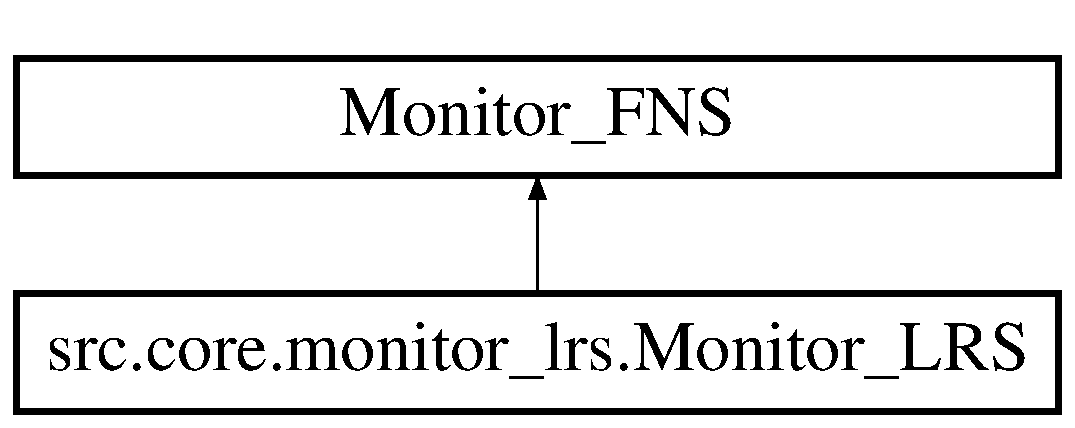
\includegraphics[height=2.000000cm]{classsrc_1_1core_1_1monitor__lrs_1_1Monitor__LRS}
\end{center}
\end{figure}
\subsection*{Public Member Functions}
\begin{DoxyCompactItemize}
\item 
def \hyperlink{classsrc_1_1core_1_1monitor__lrs_1_1Monitor__LRS_a6d3c9e648737a8d569a05af6cbd79b62}{\+\_\+\+\_\+init\+\_\+\+\_\+} (self, peer)
\item 
def \hyperlink{classsrc_1_1core_1_1monitor__lrs_1_1Monitor__LRS_a4ac336a53720b575264acd15683ace66}{receive\+\_\+the\+\_\+buffer\+\_\+size} (self)
\end{DoxyCompactItemize}
\subsection*{Public Attributes}
\begin{DoxyCompactItemize}
\item 
\hyperlink{classsrc_1_1core_1_1monitor__lrs_1_1Monitor__LRS_a888a6f9cca3db80b85e8a8b6ec9bc292}{splitter\+\_\+socket}
\item 
\hyperlink{classsrc_1_1core_1_1monitor__lrs_1_1Monitor__LRS_a2150cbf20f2b3a029adec34af31270d5}{splitter}
\item 
\hyperlink{classsrc_1_1core_1_1monitor__lrs_1_1Monitor__LRS_a9319f78256ffb9cb6aaf31e1f007e06f}{buffer\+\_\+size}
\item 
\hyperlink{classsrc_1_1core_1_1monitor__lrs_1_1Monitor__LRS_aff76930b61b20abcba04a46a92156aed}{peer\+\_\+list}
\item 
\hyperlink{classsrc_1_1core_1_1monitor__lrs_1_1Monitor__LRS_a3b26dd9994a21d6195cd1e4a9bf90aba}{player\+\_\+socket}
\item 
\hyperlink{classsrc_1_1core_1_1monitor__lrs_1_1Monitor__LRS_afc83747a7279c1119caa81a126850b0e}{chunk\+\_\+size}
\item 
\hyperlink{classsrc_1_1core_1_1monitor__lrs_1_1Monitor__LRS_a85e7a6259ff7f9f24477b259d420641a}{debt}
\item 
\hyperlink{classsrc_1_1core_1_1monitor__lrs_1_1Monitor__LRS_a9e4445cbe34150dfb5c372d2ca0bdd8d}{team\+\_\+socket}
\item 
\hyperlink{classsrc_1_1core_1_1monitor__lrs_1_1Monitor__LRS_a4a161a64b6e59bcb4ecada5b289d9b03}{message\+\_\+format}
\end{DoxyCompactItemize}


\subsection{Constructor \& Destructor Documentation}
\hypertarget{classsrc_1_1core_1_1monitor__lrs_1_1Monitor__LRS_a6d3c9e648737a8d569a05af6cbd79b62}{}\index{src\+::core\+::monitor\+\_\+lrs\+::\+Monitor\+\_\+\+L\+R\+S@{src\+::core\+::monitor\+\_\+lrs\+::\+Monitor\+\_\+\+L\+R\+S}!\+\_\+\+\_\+init\+\_\+\+\_\+@{\+\_\+\+\_\+init\+\_\+\+\_\+}}
\index{\+\_\+\+\_\+init\+\_\+\+\_\+@{\+\_\+\+\_\+init\+\_\+\+\_\+}!src\+::core\+::monitor\+\_\+lrs\+::\+Monitor\+\_\+\+L\+R\+S@{src\+::core\+::monitor\+\_\+lrs\+::\+Monitor\+\_\+\+L\+R\+S}}
\subsubsection[{\+\_\+\+\_\+init\+\_\+\+\_\+}]{\setlength{\rightskip}{0pt plus 5cm}def src.\+core.\+monitor\+\_\+lrs.\+Monitor\+\_\+\+L\+R\+S.\+\_\+\+\_\+init\+\_\+\+\_\+ (
\begin{DoxyParamCaption}
\item[{}]{self, }
\item[{}]{peer}
\end{DoxyParamCaption}
)}\label{classsrc_1_1core_1_1monitor__lrs_1_1Monitor__LRS_a6d3c9e648737a8d569a05af6cbd79b62}


\subsection{Member Function Documentation}
\hypertarget{classsrc_1_1core_1_1monitor__lrs_1_1Monitor__LRS_a4ac336a53720b575264acd15683ace66}{}\index{src\+::core\+::monitor\+\_\+lrs\+::\+Monitor\+\_\+\+L\+R\+S@{src\+::core\+::monitor\+\_\+lrs\+::\+Monitor\+\_\+\+L\+R\+S}!receive\+\_\+the\+\_\+buffer\+\_\+size@{receive\+\_\+the\+\_\+buffer\+\_\+size}}
\index{receive\+\_\+the\+\_\+buffer\+\_\+size@{receive\+\_\+the\+\_\+buffer\+\_\+size}!src\+::core\+::monitor\+\_\+lrs\+::\+Monitor\+\_\+\+L\+R\+S@{src\+::core\+::monitor\+\_\+lrs\+::\+Monitor\+\_\+\+L\+R\+S}}
\subsubsection[{receive\+\_\+the\+\_\+buffer\+\_\+size}]{\setlength{\rightskip}{0pt plus 5cm}def src.\+core.\+monitor\+\_\+lrs.\+Monitor\+\_\+\+L\+R\+S.\+receive\+\_\+the\+\_\+buffer\+\_\+size (
\begin{DoxyParamCaption}
\item[{}]{self}
\end{DoxyParamCaption}
)}\label{classsrc_1_1core_1_1monitor__lrs_1_1Monitor__LRS_a4ac336a53720b575264acd15683ace66}


\subsection{Member Data Documentation}
\hypertarget{classsrc_1_1core_1_1monitor__lrs_1_1Monitor__LRS_a9319f78256ffb9cb6aaf31e1f007e06f}{}\index{src\+::core\+::monitor\+\_\+lrs\+::\+Monitor\+\_\+\+L\+R\+S@{src\+::core\+::monitor\+\_\+lrs\+::\+Monitor\+\_\+\+L\+R\+S}!buffer\+\_\+size@{buffer\+\_\+size}}
\index{buffer\+\_\+size@{buffer\+\_\+size}!src\+::core\+::monitor\+\_\+lrs\+::\+Monitor\+\_\+\+L\+R\+S@{src\+::core\+::monitor\+\_\+lrs\+::\+Monitor\+\_\+\+L\+R\+S}}
\subsubsection[{buffer\+\_\+size}]{\setlength{\rightskip}{0pt plus 5cm}src.\+core.\+monitor\+\_\+lrs.\+Monitor\+\_\+\+L\+R\+S.\+buffer\+\_\+size}\label{classsrc_1_1core_1_1monitor__lrs_1_1Monitor__LRS_a9319f78256ffb9cb6aaf31e1f007e06f}
\hypertarget{classsrc_1_1core_1_1monitor__lrs_1_1Monitor__LRS_afc83747a7279c1119caa81a126850b0e}{}\index{src\+::core\+::monitor\+\_\+lrs\+::\+Monitor\+\_\+\+L\+R\+S@{src\+::core\+::monitor\+\_\+lrs\+::\+Monitor\+\_\+\+L\+R\+S}!chunk\+\_\+size@{chunk\+\_\+size}}
\index{chunk\+\_\+size@{chunk\+\_\+size}!src\+::core\+::monitor\+\_\+lrs\+::\+Monitor\+\_\+\+L\+R\+S@{src\+::core\+::monitor\+\_\+lrs\+::\+Monitor\+\_\+\+L\+R\+S}}
\subsubsection[{chunk\+\_\+size}]{\setlength{\rightskip}{0pt plus 5cm}src.\+core.\+monitor\+\_\+lrs.\+Monitor\+\_\+\+L\+R\+S.\+chunk\+\_\+size}\label{classsrc_1_1core_1_1monitor__lrs_1_1Monitor__LRS_afc83747a7279c1119caa81a126850b0e}
\hypertarget{classsrc_1_1core_1_1monitor__lrs_1_1Monitor__LRS_a85e7a6259ff7f9f24477b259d420641a}{}\index{src\+::core\+::monitor\+\_\+lrs\+::\+Monitor\+\_\+\+L\+R\+S@{src\+::core\+::monitor\+\_\+lrs\+::\+Monitor\+\_\+\+L\+R\+S}!debt@{debt}}
\index{debt@{debt}!src\+::core\+::monitor\+\_\+lrs\+::\+Monitor\+\_\+\+L\+R\+S@{src\+::core\+::monitor\+\_\+lrs\+::\+Monitor\+\_\+\+L\+R\+S}}
\subsubsection[{debt}]{\setlength{\rightskip}{0pt plus 5cm}src.\+core.\+monitor\+\_\+lrs.\+Monitor\+\_\+\+L\+R\+S.\+debt}\label{classsrc_1_1core_1_1monitor__lrs_1_1Monitor__LRS_a85e7a6259ff7f9f24477b259d420641a}
\hypertarget{classsrc_1_1core_1_1monitor__lrs_1_1Monitor__LRS_a4a161a64b6e59bcb4ecada5b289d9b03}{}\index{src\+::core\+::monitor\+\_\+lrs\+::\+Monitor\+\_\+\+L\+R\+S@{src\+::core\+::monitor\+\_\+lrs\+::\+Monitor\+\_\+\+L\+R\+S}!message\+\_\+format@{message\+\_\+format}}
\index{message\+\_\+format@{message\+\_\+format}!src\+::core\+::monitor\+\_\+lrs\+::\+Monitor\+\_\+\+L\+R\+S@{src\+::core\+::monitor\+\_\+lrs\+::\+Monitor\+\_\+\+L\+R\+S}}
\subsubsection[{message\+\_\+format}]{\setlength{\rightskip}{0pt plus 5cm}src.\+core.\+monitor\+\_\+lrs.\+Monitor\+\_\+\+L\+R\+S.\+message\+\_\+format}\label{classsrc_1_1core_1_1monitor__lrs_1_1Monitor__LRS_a4a161a64b6e59bcb4ecada5b289d9b03}
\hypertarget{classsrc_1_1core_1_1monitor__lrs_1_1Monitor__LRS_aff76930b61b20abcba04a46a92156aed}{}\index{src\+::core\+::monitor\+\_\+lrs\+::\+Monitor\+\_\+\+L\+R\+S@{src\+::core\+::monitor\+\_\+lrs\+::\+Monitor\+\_\+\+L\+R\+S}!peer\+\_\+list@{peer\+\_\+list}}
\index{peer\+\_\+list@{peer\+\_\+list}!src\+::core\+::monitor\+\_\+lrs\+::\+Monitor\+\_\+\+L\+R\+S@{src\+::core\+::monitor\+\_\+lrs\+::\+Monitor\+\_\+\+L\+R\+S}}
\subsubsection[{peer\+\_\+list}]{\setlength{\rightskip}{0pt plus 5cm}src.\+core.\+monitor\+\_\+lrs.\+Monitor\+\_\+\+L\+R\+S.\+peer\+\_\+list}\label{classsrc_1_1core_1_1monitor__lrs_1_1Monitor__LRS_aff76930b61b20abcba04a46a92156aed}
\hypertarget{classsrc_1_1core_1_1monitor__lrs_1_1Monitor__LRS_a3b26dd9994a21d6195cd1e4a9bf90aba}{}\index{src\+::core\+::monitor\+\_\+lrs\+::\+Monitor\+\_\+\+L\+R\+S@{src\+::core\+::monitor\+\_\+lrs\+::\+Monitor\+\_\+\+L\+R\+S}!player\+\_\+socket@{player\+\_\+socket}}
\index{player\+\_\+socket@{player\+\_\+socket}!src\+::core\+::monitor\+\_\+lrs\+::\+Monitor\+\_\+\+L\+R\+S@{src\+::core\+::monitor\+\_\+lrs\+::\+Monitor\+\_\+\+L\+R\+S}}
\subsubsection[{player\+\_\+socket}]{\setlength{\rightskip}{0pt plus 5cm}src.\+core.\+monitor\+\_\+lrs.\+Monitor\+\_\+\+L\+R\+S.\+player\+\_\+socket}\label{classsrc_1_1core_1_1monitor__lrs_1_1Monitor__LRS_a3b26dd9994a21d6195cd1e4a9bf90aba}
\hypertarget{classsrc_1_1core_1_1monitor__lrs_1_1Monitor__LRS_a2150cbf20f2b3a029adec34af31270d5}{}\index{src\+::core\+::monitor\+\_\+lrs\+::\+Monitor\+\_\+\+L\+R\+S@{src\+::core\+::monitor\+\_\+lrs\+::\+Monitor\+\_\+\+L\+R\+S}!splitter@{splitter}}
\index{splitter@{splitter}!src\+::core\+::monitor\+\_\+lrs\+::\+Monitor\+\_\+\+L\+R\+S@{src\+::core\+::monitor\+\_\+lrs\+::\+Monitor\+\_\+\+L\+R\+S}}
\subsubsection[{splitter}]{\setlength{\rightskip}{0pt plus 5cm}src.\+core.\+monitor\+\_\+lrs.\+Monitor\+\_\+\+L\+R\+S.\+splitter}\label{classsrc_1_1core_1_1monitor__lrs_1_1Monitor__LRS_a2150cbf20f2b3a029adec34af31270d5}
\hypertarget{classsrc_1_1core_1_1monitor__lrs_1_1Monitor__LRS_a888a6f9cca3db80b85e8a8b6ec9bc292}{}\index{src\+::core\+::monitor\+\_\+lrs\+::\+Monitor\+\_\+\+L\+R\+S@{src\+::core\+::monitor\+\_\+lrs\+::\+Monitor\+\_\+\+L\+R\+S}!splitter\+\_\+socket@{splitter\+\_\+socket}}
\index{splitter\+\_\+socket@{splitter\+\_\+socket}!src\+::core\+::monitor\+\_\+lrs\+::\+Monitor\+\_\+\+L\+R\+S@{src\+::core\+::monitor\+\_\+lrs\+::\+Monitor\+\_\+\+L\+R\+S}}
\subsubsection[{splitter\+\_\+socket}]{\setlength{\rightskip}{0pt plus 5cm}src.\+core.\+monitor\+\_\+lrs.\+Monitor\+\_\+\+L\+R\+S.\+splitter\+\_\+socket}\label{classsrc_1_1core_1_1monitor__lrs_1_1Monitor__LRS_a888a6f9cca3db80b85e8a8b6ec9bc292}
\hypertarget{classsrc_1_1core_1_1monitor__lrs_1_1Monitor__LRS_a9e4445cbe34150dfb5c372d2ca0bdd8d}{}\index{src\+::core\+::monitor\+\_\+lrs\+::\+Monitor\+\_\+\+L\+R\+S@{src\+::core\+::monitor\+\_\+lrs\+::\+Monitor\+\_\+\+L\+R\+S}!team\+\_\+socket@{team\+\_\+socket}}
\index{team\+\_\+socket@{team\+\_\+socket}!src\+::core\+::monitor\+\_\+lrs\+::\+Monitor\+\_\+\+L\+R\+S@{src\+::core\+::monitor\+\_\+lrs\+::\+Monitor\+\_\+\+L\+R\+S}}
\subsubsection[{team\+\_\+socket}]{\setlength{\rightskip}{0pt plus 5cm}src.\+core.\+monitor\+\_\+lrs.\+Monitor\+\_\+\+L\+R\+S.\+team\+\_\+socket}\label{classsrc_1_1core_1_1monitor__lrs_1_1Monitor__LRS_a9e4445cbe34150dfb5c372d2ca0bdd8d}


The documentation for this class was generated from the following file\+:\begin{DoxyCompactItemize}
\item 
src/core/\hyperlink{monitor__lrs_8py}{monitor\+\_\+lrs.\+py}\end{DoxyCompactItemize}

\hypertarget{classsrc_1_1lib_1_1vlc_1_1NavigateMode}{}\section{src.\+lib.\+vlc.\+Navigate\+Mode Class Reference}
\label{classsrc_1_1lib_1_1vlc_1_1NavigateMode}\index{src.\+lib.\+vlc.\+Navigate\+Mode@{src.\+lib.\+vlc.\+Navigate\+Mode}}
Inheritance diagram for src.\+lib.\+vlc.\+Navigate\+Mode\+:\begin{figure}[H]
\begin{center}
\leavevmode
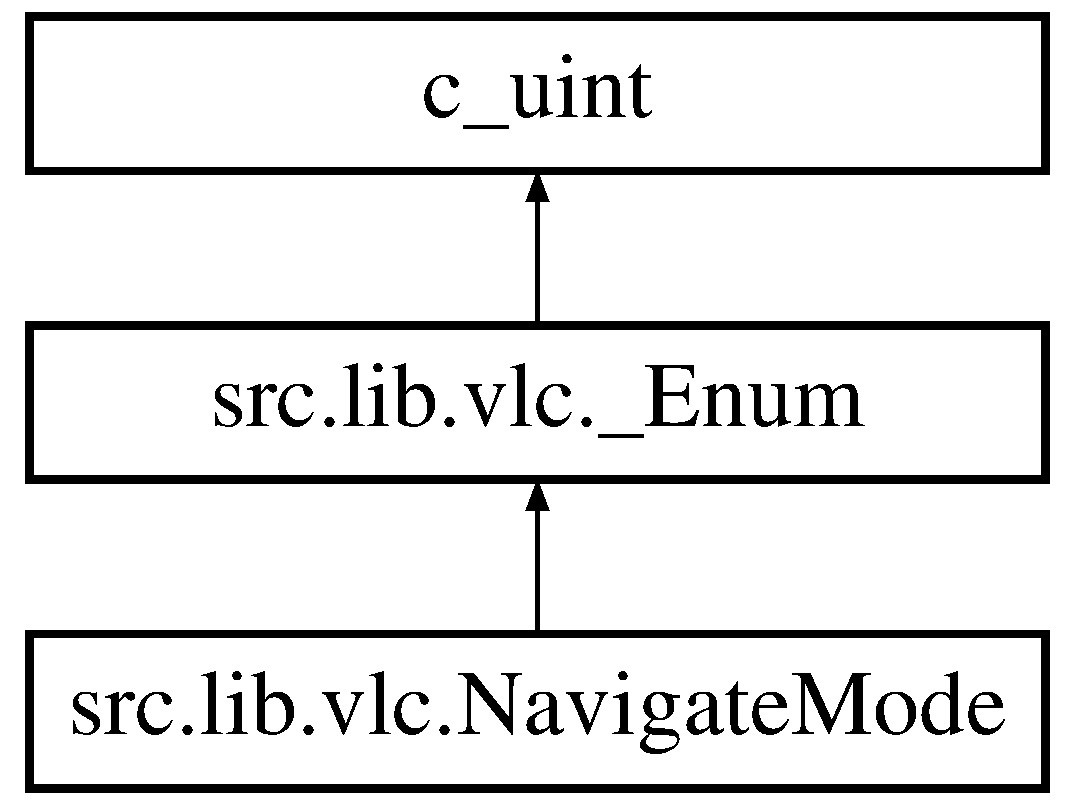
\includegraphics[height=3.000000cm]{classsrc_1_1lib_1_1vlc_1_1NavigateMode}
\end{center}
\end{figure}
\subsection*{Static Private Attributes}
\begin{DoxyCompactItemize}
\item 
dictionary \hyperlink{classsrc_1_1lib_1_1vlc_1_1NavigateMode_a6bd87d39ccd020c4b4a2e31189764bc5}{\+\_\+enum\+\_\+names\+\_\+}
\end{DoxyCompactItemize}
\subsection*{Additional Inherited Members}


\subsection{Detailed Description}
\begin{DoxyVerb}Navigation mode.
\end{DoxyVerb}
 

\subsection{Member Data Documentation}
\hypertarget{classsrc_1_1lib_1_1vlc_1_1NavigateMode_a6bd87d39ccd020c4b4a2e31189764bc5}{}\index{src\+::lib\+::vlc\+::\+Navigate\+Mode@{src\+::lib\+::vlc\+::\+Navigate\+Mode}!\+\_\+enum\+\_\+names\+\_\+@{\+\_\+enum\+\_\+names\+\_\+}}
\index{\+\_\+enum\+\_\+names\+\_\+@{\+\_\+enum\+\_\+names\+\_\+}!src\+::lib\+::vlc\+::\+Navigate\+Mode@{src\+::lib\+::vlc\+::\+Navigate\+Mode}}
\subsubsection[{\+\_\+enum\+\_\+names\+\_\+}]{\setlength{\rightskip}{0pt plus 5cm}dictionary src.\+lib.\+vlc.\+Navigate\+Mode.\+\_\+enum\+\_\+names\+\_\+\hspace{0.3cm}{\ttfamily [static]}, {\ttfamily [private]}}\label{classsrc_1_1lib_1_1vlc_1_1NavigateMode_a6bd87d39ccd020c4b4a2e31189764bc5}
{\bfseries Initial value\+:}
\begin{DoxyCode}
1 = \{
2         0: \textcolor{stringliteral}{'activate'},
3         1: \textcolor{stringliteral}{'up'},
4         2: \textcolor{stringliteral}{'down'},
5         3: \textcolor{stringliteral}{'left'},
6         4: \textcolor{stringliteral}{'right'},
7     \}
\end{DoxyCode}


The documentation for this class was generated from the following file\+:\begin{DoxyCompactItemize}
\item 
src/lib/\hyperlink{vlc_8py}{vlc.\+py}\end{DoxyCompactItemize}

\hypertarget{classtest__UDP_1_1Packets__per__second}{}\section{test\+\_\+\+U\+D\+P.\+Packets\+\_\+per\+\_\+second Class Reference}
\label{classtest__UDP_1_1Packets__per__second}\index{test\+\_\+\+U\+D\+P.\+Packets\+\_\+per\+\_\+second@{test\+\_\+\+U\+D\+P.\+Packets\+\_\+per\+\_\+second}}
Inheritance diagram for test\+\_\+\+U\+D\+P.\+Packets\+\_\+per\+\_\+second\+:\begin{figure}[H]
\begin{center}
\leavevmode
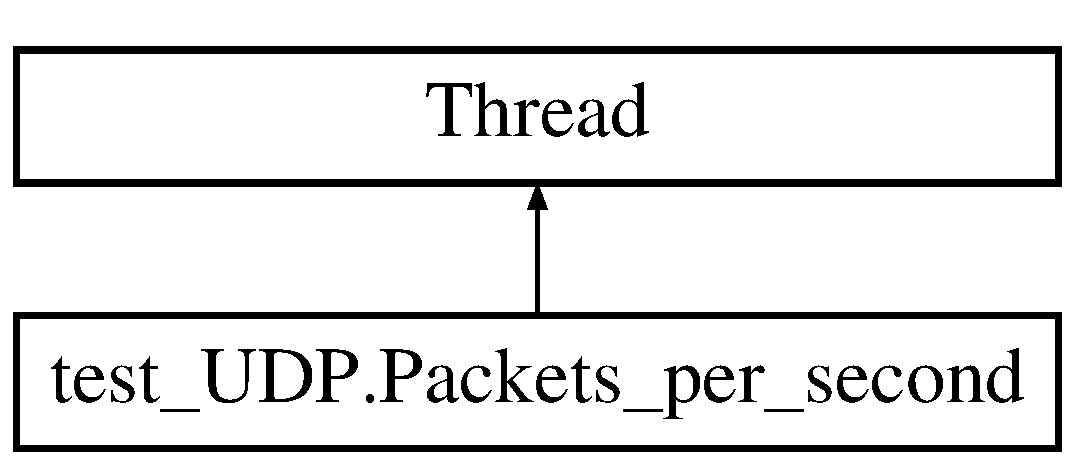
\includegraphics[height=2.000000cm]{classtest__UDP_1_1Packets__per__second}
\end{center}
\end{figure}
\subsection*{Public Member Functions}
\begin{DoxyCompactItemize}
\item 
def \hyperlink{classtest__UDP_1_1Packets__per__second_af7608284cc040fed1c76d21c0a7ac398}{\+\_\+\+\_\+init\+\_\+\+\_\+} (self)
\item 
def \hyperlink{classtest__UDP_1_1Packets__per__second_a990aad55d0bec600458cdaf64d99f3ce}{run} (self)
\end{DoxyCompactItemize}


\subsection{Constructor \& Destructor Documentation}
\hypertarget{classtest__UDP_1_1Packets__per__second_af7608284cc040fed1c76d21c0a7ac398}{}\index{test\+\_\+\+U\+D\+P\+::\+Packets\+\_\+per\+\_\+second@{test\+\_\+\+U\+D\+P\+::\+Packets\+\_\+per\+\_\+second}!\+\_\+\+\_\+init\+\_\+\+\_\+@{\+\_\+\+\_\+init\+\_\+\+\_\+}}
\index{\+\_\+\+\_\+init\+\_\+\+\_\+@{\+\_\+\+\_\+init\+\_\+\+\_\+}!test\+\_\+\+U\+D\+P\+::\+Packets\+\_\+per\+\_\+second@{test\+\_\+\+U\+D\+P\+::\+Packets\+\_\+per\+\_\+second}}
\subsubsection[{\+\_\+\+\_\+init\+\_\+\+\_\+}]{\setlength{\rightskip}{0pt plus 5cm}def test\+\_\+\+U\+D\+P.\+Packets\+\_\+per\+\_\+second.\+\_\+\+\_\+init\+\_\+\+\_\+ (
\begin{DoxyParamCaption}
\item[{}]{self}
\end{DoxyParamCaption}
)}\label{classtest__UDP_1_1Packets__per__second_af7608284cc040fed1c76d21c0a7ac398}


\subsection{Member Function Documentation}
\hypertarget{classtest__UDP_1_1Packets__per__second_a990aad55d0bec600458cdaf64d99f3ce}{}\index{test\+\_\+\+U\+D\+P\+::\+Packets\+\_\+per\+\_\+second@{test\+\_\+\+U\+D\+P\+::\+Packets\+\_\+per\+\_\+second}!run@{run}}
\index{run@{run}!test\+\_\+\+U\+D\+P\+::\+Packets\+\_\+per\+\_\+second@{test\+\_\+\+U\+D\+P\+::\+Packets\+\_\+per\+\_\+second}}
\subsubsection[{run}]{\setlength{\rightskip}{0pt plus 5cm}def test\+\_\+\+U\+D\+P.\+Packets\+\_\+per\+\_\+second.\+run (
\begin{DoxyParamCaption}
\item[{}]{self}
\end{DoxyParamCaption}
)}\label{classtest__UDP_1_1Packets__per__second_a990aad55d0bec600458cdaf64d99f3ce}


The documentation for this class was generated from the following file\+:\begin{DoxyCompactItemize}
\item 
tools/\hyperlink{test__UDP_8py}{test\+\_\+\+U\+D\+P.\+py}\end{DoxyCompactItemize}

\hypertarget{classsrc_1_1core_1_1peer_1_1Peer}{}\section{src.\+core.\+peer.\+Peer Class Reference}
\label{classsrc_1_1core_1_1peer_1_1Peer}\index{src.\+core.\+peer.\+Peer@{src.\+core.\+peer.\+Peer}}
\subsection*{Public Member Functions}
\begin{DoxyCompactItemize}
\item 
def \hyperlink{classsrc_1_1core_1_1peer_1_1Peer_a6ce21bf8f6d869cd470efd714ed2d558}{\+\_\+\+\_\+init\+\_\+\+\_\+} (self)
\end{DoxyCompactItemize}


\subsection{Constructor \& Destructor Documentation}
\hypertarget{classsrc_1_1core_1_1peer_1_1Peer_a6ce21bf8f6d869cd470efd714ed2d558}{}\index{src\+::core\+::peer\+::\+Peer@{src\+::core\+::peer\+::\+Peer}!\+\_\+\+\_\+init\+\_\+\+\_\+@{\+\_\+\+\_\+init\+\_\+\+\_\+}}
\index{\+\_\+\+\_\+init\+\_\+\+\_\+@{\+\_\+\+\_\+init\+\_\+\+\_\+}!src\+::core\+::peer\+::\+Peer@{src\+::core\+::peer\+::\+Peer}}
\subsubsection[{\+\_\+\+\_\+init\+\_\+\+\_\+}]{\setlength{\rightskip}{0pt plus 5cm}def src.\+core.\+peer.\+Peer.\+\_\+\+\_\+init\+\_\+\+\_\+ (
\begin{DoxyParamCaption}
\item[{}]{self}
\end{DoxyParamCaption}
)}\label{classsrc_1_1core_1_1peer_1_1Peer_a6ce21bf8f6d869cd470efd714ed2d558}


The documentation for this class was generated from the following file\+:\begin{DoxyCompactItemize}
\item 
src/core/\hyperlink{peer_8py}{peer.\+py}\end{DoxyCompactItemize}

\hypertarget{classsrc_1_1core_1_1peer__dbs_1_1Peer__DBS}{}\section{src.\+core.\+peer\+\_\+dbs.\+Peer\+\_\+\+D\+B\+S Class Reference}
\label{classsrc_1_1core_1_1peer__dbs_1_1Peer__DBS}\index{src.\+core.\+peer\+\_\+dbs.\+Peer\+\_\+\+D\+B\+S@{src.\+core.\+peer\+\_\+dbs.\+Peer\+\_\+\+D\+B\+S}}
Inheritance diagram for src.\+core.\+peer\+\_\+dbs.\+Peer\+\_\+\+D\+B\+S\+:\begin{figure}[H]
\begin{center}
\leavevmode
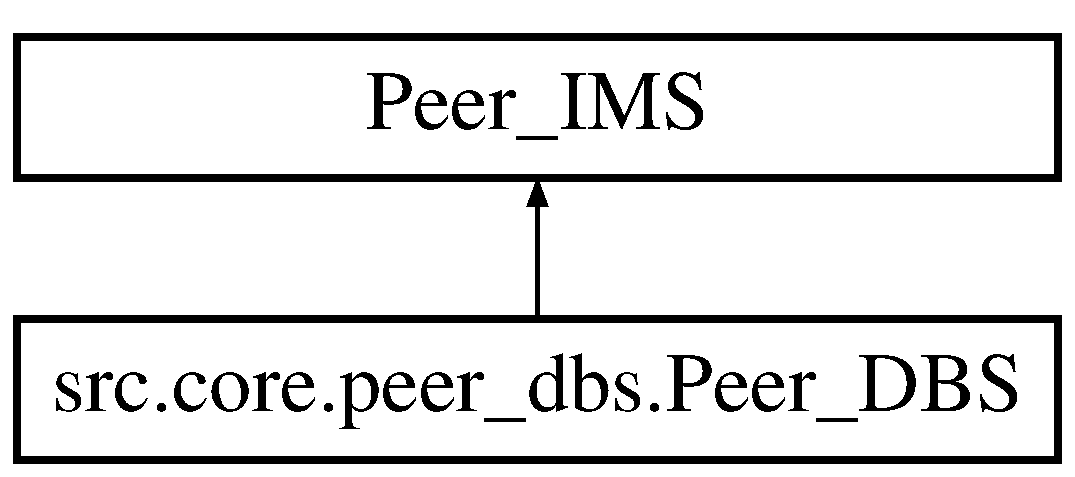
\includegraphics[height=2.000000cm]{classsrc_1_1core_1_1peer__dbs_1_1Peer__DBS}
\end{center}
\end{figure}
\subsection*{Public Member Functions}
\begin{DoxyCompactItemize}
\item 
def \hyperlink{classsrc_1_1core_1_1peer__dbs_1_1Peer__DBS_a41411fc6be8f7bfd13359ff180ff7d2f}{\+\_\+\+\_\+init\+\_\+\+\_\+} (self, peer)
\item 
def \hyperlink{classsrc_1_1core_1_1peer__dbs_1_1Peer__DBS_a2d708a217f203bda30921e5511ecb9a8}{say\+\_\+hello} (self, node)
\item 
def \hyperlink{classsrc_1_1core_1_1peer__dbs_1_1Peer__DBS_a489ca58c6aa79b47c6ebb9d2f3267348}{say\+\_\+goodbye} (self, node)
\item 
def \hyperlink{classsrc_1_1core_1_1peer__dbs_1_1Peer__DBS_a4fca27fc0794095d160ea3893876c1f8}{receive\+\_\+the\+\_\+number\+\_\+of\+\_\+peers} (self)
\item 
def \hyperlink{classsrc_1_1core_1_1peer__dbs_1_1Peer__DBS_ade29498101146c58d82e451267b24e32}{receive\+\_\+the\+\_\+list\+\_\+of\+\_\+peers} (self)
\item 
def \hyperlink{classsrc_1_1core_1_1peer__dbs_1_1Peer__DBS_aed0fd93df0126054ea2f26fe26a5aa46}{receive\+\_\+my\+\_\+endpoint} (self)
\item 
def \hyperlink{classsrc_1_1core_1_1peer__dbs_1_1Peer__DBS_a420335be06084664f7822735825d7f17}{listen\+\_\+to\+\_\+the\+\_\+team} (self)
\item 
def \hyperlink{classsrc_1_1core_1_1peer__dbs_1_1Peer__DBS_aae3e8cf37a751f2441440f139f1bdfa1}{process\+\_\+next\+\_\+message} (self)
\item 
def \hyperlink{classsrc_1_1core_1_1peer__dbs_1_1Peer__DBS_ad05c1cdcb376412d8aa46297d5c8943a}{keep\+\_\+the\+\_\+buffer\+\_\+full} (self)
\item 
def \hyperlink{classsrc_1_1core_1_1peer__dbs_1_1Peer__DBS_a8b111a1fafae5086bfdbc2cf9e7d0460}{polite\+\_\+farewell} (self)
\item 
def \hyperlink{classsrc_1_1core_1_1peer__dbs_1_1Peer__DBS_a732495ad69f86f0b105f115e73c688f7}{buffer\+\_\+data} (self)
\item 
def \hyperlink{classsrc_1_1core_1_1peer__dbs_1_1Peer__DBS_a11676ccd7989c8b282573fe0e4c8d3dc}{run} (self)
\item 
def \hyperlink{classsrc_1_1core_1_1peer__dbs_1_1Peer__DBS_ae9b897f5b62eab99fc3efe4f005fa5b5}{am\+\_\+i\+\_\+a\+\_\+monitor} (self)
\end{DoxyCompactItemize}
\subsection*{Public Attributes}
\begin{DoxyCompactItemize}
\item 
\hyperlink{classsrc_1_1core_1_1peer__dbs_1_1Peer__DBS_a20f9c699a4f21deb815b18b66a9f0a15}{splitter\+\_\+socket}
\item 
\hyperlink{classsrc_1_1core_1_1peer__dbs_1_1Peer__DBS_ac9c680d2156271762889ca8df74d8729}{player\+\_\+socket}
\item 
\hyperlink{classsrc_1_1core_1_1peer__dbs_1_1Peer__DBS_a40aeb00ce0d74c866a44cae0832cb627}{buffer\+\_\+size}
\item 
\hyperlink{classsrc_1_1core_1_1peer__dbs_1_1Peer__DBS_ac893e7587632b197d5867d72f8665721}{splitter}
\item 
\hyperlink{classsrc_1_1core_1_1peer__dbs_1_1Peer__DBS_a4e59f03402531dff3b8dab83a78ab1a2}{chunk\+\_\+size}
\item 
\hyperlink{classsrc_1_1core_1_1peer__dbs_1_1Peer__DBS_a35425ace8df8bc35ca5ca9d17c46b813}{message\+\_\+format}
\item 
\hyperlink{classsrc_1_1core_1_1peer__dbs_1_1Peer__DBS_a73d19818ef068e8dcb055aa16621e367}{debt}
\item 
\hyperlink{classsrc_1_1core_1_1peer__dbs_1_1Peer__DBS_a8bc92e8755ed4c4f9e4362a80a39991a}{peer\+\_\+list}
\item 
\hyperlink{classsrc_1_1core_1_1peer__dbs_1_1Peer__DBS_ae2066ca8afc595638a2f545c744c77d0}{number\+\_\+of\+\_\+peers}
\item 
\hyperlink{classsrc_1_1core_1_1peer__dbs_1_1Peer__DBS_a305a94f69a6e54994164fed3804e3068}{me}
\item 
\hyperlink{classsrc_1_1core_1_1peer__dbs_1_1Peer__DBS_acf4415c5d44af6904b83bfe873c4b0c7}{team\+\_\+socket}
\item 
\hyperlink{classsrc_1_1core_1_1peer__dbs_1_1Peer__DBS_af6d5a5c7d7e437a34367b3386172a18b}{receive\+\_\+and\+\_\+feed\+\_\+counter}
\item 
\hyperlink{classsrc_1_1core_1_1peer__dbs_1_1Peer__DBS_a89f4aab576119eec74a32db571b54c77}{receive\+\_\+and\+\_\+feed\+\_\+previous}
\item 
\hyperlink{classsrc_1_1core_1_1peer__dbs_1_1Peer__DBS_ab26d64535b00ba7488db5fcf51cdfda4}{sendto\+\_\+counter}
\item 
\hyperlink{classsrc_1_1core_1_1peer__dbs_1_1Peer__DBS_a0bf552827e8d0e698337bd89741cef27}{debt\+\_\+memory}
\end{DoxyCompactItemize}
\subsection*{Static Public Attributes}
\begin{DoxyCompactItemize}
\item 
int \hyperlink{classsrc_1_1core_1_1peer__dbs_1_1Peer__DBS_a7ae18c2cdc85bc1cece62d05e71c25dc}{M\+A\+X\+\_\+\+C\+H\+U\+N\+K\+\_\+\+D\+E\+B\+T} = 128
\end{DoxyCompactItemize}


\subsection{Constructor \& Destructor Documentation}
\hypertarget{classsrc_1_1core_1_1peer__dbs_1_1Peer__DBS_a41411fc6be8f7bfd13359ff180ff7d2f}{}\index{src\+::core\+::peer\+\_\+dbs\+::\+Peer\+\_\+\+D\+B\+S@{src\+::core\+::peer\+\_\+dbs\+::\+Peer\+\_\+\+D\+B\+S}!\+\_\+\+\_\+init\+\_\+\+\_\+@{\+\_\+\+\_\+init\+\_\+\+\_\+}}
\index{\+\_\+\+\_\+init\+\_\+\+\_\+@{\+\_\+\+\_\+init\+\_\+\+\_\+}!src\+::core\+::peer\+\_\+dbs\+::\+Peer\+\_\+\+D\+B\+S@{src\+::core\+::peer\+\_\+dbs\+::\+Peer\+\_\+\+D\+B\+S}}
\subsubsection[{\+\_\+\+\_\+init\+\_\+\+\_\+}]{\setlength{\rightskip}{0pt plus 5cm}def src.\+core.\+peer\+\_\+dbs.\+Peer\+\_\+\+D\+B\+S.\+\_\+\+\_\+init\+\_\+\+\_\+ (
\begin{DoxyParamCaption}
\item[{}]{self, }
\item[{}]{peer}
\end{DoxyParamCaption}
)}\label{classsrc_1_1core_1_1peer__dbs_1_1Peer__DBS_a41411fc6be8f7bfd13359ff180ff7d2f}


\subsection{Member Function Documentation}
\hypertarget{classsrc_1_1core_1_1peer__dbs_1_1Peer__DBS_ae9b897f5b62eab99fc3efe4f005fa5b5}{}\index{src\+::core\+::peer\+\_\+dbs\+::\+Peer\+\_\+\+D\+B\+S@{src\+::core\+::peer\+\_\+dbs\+::\+Peer\+\_\+\+D\+B\+S}!am\+\_\+i\+\_\+a\+\_\+monitor@{am\+\_\+i\+\_\+a\+\_\+monitor}}
\index{am\+\_\+i\+\_\+a\+\_\+monitor@{am\+\_\+i\+\_\+a\+\_\+monitor}!src\+::core\+::peer\+\_\+dbs\+::\+Peer\+\_\+\+D\+B\+S@{src\+::core\+::peer\+\_\+dbs\+::\+Peer\+\_\+\+D\+B\+S}}
\subsubsection[{am\+\_\+i\+\_\+a\+\_\+monitor}]{\setlength{\rightskip}{0pt plus 5cm}def src.\+core.\+peer\+\_\+dbs.\+Peer\+\_\+\+D\+B\+S.\+am\+\_\+i\+\_\+a\+\_\+monitor (
\begin{DoxyParamCaption}
\item[{}]{self}
\end{DoxyParamCaption}
)}\label{classsrc_1_1core_1_1peer__dbs_1_1Peer__DBS_ae9b897f5b62eab99fc3efe4f005fa5b5}
\hypertarget{classsrc_1_1core_1_1peer__dbs_1_1Peer__DBS_a732495ad69f86f0b105f115e73c688f7}{}\index{src\+::core\+::peer\+\_\+dbs\+::\+Peer\+\_\+\+D\+B\+S@{src\+::core\+::peer\+\_\+dbs\+::\+Peer\+\_\+\+D\+B\+S}!buffer\+\_\+data@{buffer\+\_\+data}}
\index{buffer\+\_\+data@{buffer\+\_\+data}!src\+::core\+::peer\+\_\+dbs\+::\+Peer\+\_\+\+D\+B\+S@{src\+::core\+::peer\+\_\+dbs\+::\+Peer\+\_\+\+D\+B\+S}}
\subsubsection[{buffer\+\_\+data}]{\setlength{\rightskip}{0pt plus 5cm}def src.\+core.\+peer\+\_\+dbs.\+Peer\+\_\+\+D\+B\+S.\+buffer\+\_\+data (
\begin{DoxyParamCaption}
\item[{}]{self}
\end{DoxyParamCaption}
)}\label{classsrc_1_1core_1_1peer__dbs_1_1Peer__DBS_a732495ad69f86f0b105f115e73c688f7}
\hypertarget{classsrc_1_1core_1_1peer__dbs_1_1Peer__DBS_ad05c1cdcb376412d8aa46297d5c8943a}{}\index{src\+::core\+::peer\+\_\+dbs\+::\+Peer\+\_\+\+D\+B\+S@{src\+::core\+::peer\+\_\+dbs\+::\+Peer\+\_\+\+D\+B\+S}!keep\+\_\+the\+\_\+buffer\+\_\+full@{keep\+\_\+the\+\_\+buffer\+\_\+full}}
\index{keep\+\_\+the\+\_\+buffer\+\_\+full@{keep\+\_\+the\+\_\+buffer\+\_\+full}!src\+::core\+::peer\+\_\+dbs\+::\+Peer\+\_\+\+D\+B\+S@{src\+::core\+::peer\+\_\+dbs\+::\+Peer\+\_\+\+D\+B\+S}}
\subsubsection[{keep\+\_\+the\+\_\+buffer\+\_\+full}]{\setlength{\rightskip}{0pt plus 5cm}def src.\+core.\+peer\+\_\+dbs.\+Peer\+\_\+\+D\+B\+S.\+keep\+\_\+the\+\_\+buffer\+\_\+full (
\begin{DoxyParamCaption}
\item[{}]{self}
\end{DoxyParamCaption}
)}\label{classsrc_1_1core_1_1peer__dbs_1_1Peer__DBS_ad05c1cdcb376412d8aa46297d5c8943a}
\hypertarget{classsrc_1_1core_1_1peer__dbs_1_1Peer__DBS_a420335be06084664f7822735825d7f17}{}\index{src\+::core\+::peer\+\_\+dbs\+::\+Peer\+\_\+\+D\+B\+S@{src\+::core\+::peer\+\_\+dbs\+::\+Peer\+\_\+\+D\+B\+S}!listen\+\_\+to\+\_\+the\+\_\+team@{listen\+\_\+to\+\_\+the\+\_\+team}}
\index{listen\+\_\+to\+\_\+the\+\_\+team@{listen\+\_\+to\+\_\+the\+\_\+team}!src\+::core\+::peer\+\_\+dbs\+::\+Peer\+\_\+\+D\+B\+S@{src\+::core\+::peer\+\_\+dbs\+::\+Peer\+\_\+\+D\+B\+S}}
\subsubsection[{listen\+\_\+to\+\_\+the\+\_\+team}]{\setlength{\rightskip}{0pt plus 5cm}def src.\+core.\+peer\+\_\+dbs.\+Peer\+\_\+\+D\+B\+S.\+listen\+\_\+to\+\_\+the\+\_\+team (
\begin{DoxyParamCaption}
\item[{}]{self}
\end{DoxyParamCaption}
)}\label{classsrc_1_1core_1_1peer__dbs_1_1Peer__DBS_a420335be06084664f7822735825d7f17}
\hypertarget{classsrc_1_1core_1_1peer__dbs_1_1Peer__DBS_a8b111a1fafae5086bfdbc2cf9e7d0460}{}\index{src\+::core\+::peer\+\_\+dbs\+::\+Peer\+\_\+\+D\+B\+S@{src\+::core\+::peer\+\_\+dbs\+::\+Peer\+\_\+\+D\+B\+S}!polite\+\_\+farewell@{polite\+\_\+farewell}}
\index{polite\+\_\+farewell@{polite\+\_\+farewell}!src\+::core\+::peer\+\_\+dbs\+::\+Peer\+\_\+\+D\+B\+S@{src\+::core\+::peer\+\_\+dbs\+::\+Peer\+\_\+\+D\+B\+S}}
\subsubsection[{polite\+\_\+farewell}]{\setlength{\rightskip}{0pt plus 5cm}def src.\+core.\+peer\+\_\+dbs.\+Peer\+\_\+\+D\+B\+S.\+polite\+\_\+farewell (
\begin{DoxyParamCaption}
\item[{}]{self}
\end{DoxyParamCaption}
)}\label{classsrc_1_1core_1_1peer__dbs_1_1Peer__DBS_a8b111a1fafae5086bfdbc2cf9e7d0460}
\hypertarget{classsrc_1_1core_1_1peer__dbs_1_1Peer__DBS_aae3e8cf37a751f2441440f139f1bdfa1}{}\index{src\+::core\+::peer\+\_\+dbs\+::\+Peer\+\_\+\+D\+B\+S@{src\+::core\+::peer\+\_\+dbs\+::\+Peer\+\_\+\+D\+B\+S}!process\+\_\+next\+\_\+message@{process\+\_\+next\+\_\+message}}
\index{process\+\_\+next\+\_\+message@{process\+\_\+next\+\_\+message}!src\+::core\+::peer\+\_\+dbs\+::\+Peer\+\_\+\+D\+B\+S@{src\+::core\+::peer\+\_\+dbs\+::\+Peer\+\_\+\+D\+B\+S}}
\subsubsection[{process\+\_\+next\+\_\+message}]{\setlength{\rightskip}{0pt plus 5cm}def src.\+core.\+peer\+\_\+dbs.\+Peer\+\_\+\+D\+B\+S.\+process\+\_\+next\+\_\+message (
\begin{DoxyParamCaption}
\item[{}]{self}
\end{DoxyParamCaption}
)}\label{classsrc_1_1core_1_1peer__dbs_1_1Peer__DBS_aae3e8cf37a751f2441440f139f1bdfa1}
\hypertarget{classsrc_1_1core_1_1peer__dbs_1_1Peer__DBS_aed0fd93df0126054ea2f26fe26a5aa46}{}\index{src\+::core\+::peer\+\_\+dbs\+::\+Peer\+\_\+\+D\+B\+S@{src\+::core\+::peer\+\_\+dbs\+::\+Peer\+\_\+\+D\+B\+S}!receive\+\_\+my\+\_\+endpoint@{receive\+\_\+my\+\_\+endpoint}}
\index{receive\+\_\+my\+\_\+endpoint@{receive\+\_\+my\+\_\+endpoint}!src\+::core\+::peer\+\_\+dbs\+::\+Peer\+\_\+\+D\+B\+S@{src\+::core\+::peer\+\_\+dbs\+::\+Peer\+\_\+\+D\+B\+S}}
\subsubsection[{receive\+\_\+my\+\_\+endpoint}]{\setlength{\rightskip}{0pt plus 5cm}def src.\+core.\+peer\+\_\+dbs.\+Peer\+\_\+\+D\+B\+S.\+receive\+\_\+my\+\_\+endpoint (
\begin{DoxyParamCaption}
\item[{}]{self}
\end{DoxyParamCaption}
)}\label{classsrc_1_1core_1_1peer__dbs_1_1Peer__DBS_aed0fd93df0126054ea2f26fe26a5aa46}
\hypertarget{classsrc_1_1core_1_1peer__dbs_1_1Peer__DBS_ade29498101146c58d82e451267b24e32}{}\index{src\+::core\+::peer\+\_\+dbs\+::\+Peer\+\_\+\+D\+B\+S@{src\+::core\+::peer\+\_\+dbs\+::\+Peer\+\_\+\+D\+B\+S}!receive\+\_\+the\+\_\+list\+\_\+of\+\_\+peers@{receive\+\_\+the\+\_\+list\+\_\+of\+\_\+peers}}
\index{receive\+\_\+the\+\_\+list\+\_\+of\+\_\+peers@{receive\+\_\+the\+\_\+list\+\_\+of\+\_\+peers}!src\+::core\+::peer\+\_\+dbs\+::\+Peer\+\_\+\+D\+B\+S@{src\+::core\+::peer\+\_\+dbs\+::\+Peer\+\_\+\+D\+B\+S}}
\subsubsection[{receive\+\_\+the\+\_\+list\+\_\+of\+\_\+peers}]{\setlength{\rightskip}{0pt plus 5cm}def src.\+core.\+peer\+\_\+dbs.\+Peer\+\_\+\+D\+B\+S.\+receive\+\_\+the\+\_\+list\+\_\+of\+\_\+peers (
\begin{DoxyParamCaption}
\item[{}]{self}
\end{DoxyParamCaption}
)}\label{classsrc_1_1core_1_1peer__dbs_1_1Peer__DBS_ade29498101146c58d82e451267b24e32}
\hypertarget{classsrc_1_1core_1_1peer__dbs_1_1Peer__DBS_a4fca27fc0794095d160ea3893876c1f8}{}\index{src\+::core\+::peer\+\_\+dbs\+::\+Peer\+\_\+\+D\+B\+S@{src\+::core\+::peer\+\_\+dbs\+::\+Peer\+\_\+\+D\+B\+S}!receive\+\_\+the\+\_\+number\+\_\+of\+\_\+peers@{receive\+\_\+the\+\_\+number\+\_\+of\+\_\+peers}}
\index{receive\+\_\+the\+\_\+number\+\_\+of\+\_\+peers@{receive\+\_\+the\+\_\+number\+\_\+of\+\_\+peers}!src\+::core\+::peer\+\_\+dbs\+::\+Peer\+\_\+\+D\+B\+S@{src\+::core\+::peer\+\_\+dbs\+::\+Peer\+\_\+\+D\+B\+S}}
\subsubsection[{receive\+\_\+the\+\_\+number\+\_\+of\+\_\+peers}]{\setlength{\rightskip}{0pt plus 5cm}def src.\+core.\+peer\+\_\+dbs.\+Peer\+\_\+\+D\+B\+S.\+receive\+\_\+the\+\_\+number\+\_\+of\+\_\+peers (
\begin{DoxyParamCaption}
\item[{}]{self}
\end{DoxyParamCaption}
)}\label{classsrc_1_1core_1_1peer__dbs_1_1Peer__DBS_a4fca27fc0794095d160ea3893876c1f8}
\hypertarget{classsrc_1_1core_1_1peer__dbs_1_1Peer__DBS_a11676ccd7989c8b282573fe0e4c8d3dc}{}\index{src\+::core\+::peer\+\_\+dbs\+::\+Peer\+\_\+\+D\+B\+S@{src\+::core\+::peer\+\_\+dbs\+::\+Peer\+\_\+\+D\+B\+S}!run@{run}}
\index{run@{run}!src\+::core\+::peer\+\_\+dbs\+::\+Peer\+\_\+\+D\+B\+S@{src\+::core\+::peer\+\_\+dbs\+::\+Peer\+\_\+\+D\+B\+S}}
\subsubsection[{run}]{\setlength{\rightskip}{0pt plus 5cm}def src.\+core.\+peer\+\_\+dbs.\+Peer\+\_\+\+D\+B\+S.\+run (
\begin{DoxyParamCaption}
\item[{}]{self}
\end{DoxyParamCaption}
)}\label{classsrc_1_1core_1_1peer__dbs_1_1Peer__DBS_a11676ccd7989c8b282573fe0e4c8d3dc}
\hypertarget{classsrc_1_1core_1_1peer__dbs_1_1Peer__DBS_a489ca58c6aa79b47c6ebb9d2f3267348}{}\index{src\+::core\+::peer\+\_\+dbs\+::\+Peer\+\_\+\+D\+B\+S@{src\+::core\+::peer\+\_\+dbs\+::\+Peer\+\_\+\+D\+B\+S}!say\+\_\+goodbye@{say\+\_\+goodbye}}
\index{say\+\_\+goodbye@{say\+\_\+goodbye}!src\+::core\+::peer\+\_\+dbs\+::\+Peer\+\_\+\+D\+B\+S@{src\+::core\+::peer\+\_\+dbs\+::\+Peer\+\_\+\+D\+B\+S}}
\subsubsection[{say\+\_\+goodbye}]{\setlength{\rightskip}{0pt plus 5cm}def src.\+core.\+peer\+\_\+dbs.\+Peer\+\_\+\+D\+B\+S.\+say\+\_\+goodbye (
\begin{DoxyParamCaption}
\item[{}]{self, }
\item[{}]{node}
\end{DoxyParamCaption}
)}\label{classsrc_1_1core_1_1peer__dbs_1_1Peer__DBS_a489ca58c6aa79b47c6ebb9d2f3267348}
\hypertarget{classsrc_1_1core_1_1peer__dbs_1_1Peer__DBS_a2d708a217f203bda30921e5511ecb9a8}{}\index{src\+::core\+::peer\+\_\+dbs\+::\+Peer\+\_\+\+D\+B\+S@{src\+::core\+::peer\+\_\+dbs\+::\+Peer\+\_\+\+D\+B\+S}!say\+\_\+hello@{say\+\_\+hello}}
\index{say\+\_\+hello@{say\+\_\+hello}!src\+::core\+::peer\+\_\+dbs\+::\+Peer\+\_\+\+D\+B\+S@{src\+::core\+::peer\+\_\+dbs\+::\+Peer\+\_\+\+D\+B\+S}}
\subsubsection[{say\+\_\+hello}]{\setlength{\rightskip}{0pt plus 5cm}def src.\+core.\+peer\+\_\+dbs.\+Peer\+\_\+\+D\+B\+S.\+say\+\_\+hello (
\begin{DoxyParamCaption}
\item[{}]{self, }
\item[{}]{node}
\end{DoxyParamCaption}
)}\label{classsrc_1_1core_1_1peer__dbs_1_1Peer__DBS_a2d708a217f203bda30921e5511ecb9a8}


\subsection{Member Data Documentation}
\hypertarget{classsrc_1_1core_1_1peer__dbs_1_1Peer__DBS_a40aeb00ce0d74c866a44cae0832cb627}{}\index{src\+::core\+::peer\+\_\+dbs\+::\+Peer\+\_\+\+D\+B\+S@{src\+::core\+::peer\+\_\+dbs\+::\+Peer\+\_\+\+D\+B\+S}!buffer\+\_\+size@{buffer\+\_\+size}}
\index{buffer\+\_\+size@{buffer\+\_\+size}!src\+::core\+::peer\+\_\+dbs\+::\+Peer\+\_\+\+D\+B\+S@{src\+::core\+::peer\+\_\+dbs\+::\+Peer\+\_\+\+D\+B\+S}}
\subsubsection[{buffer\+\_\+size}]{\setlength{\rightskip}{0pt plus 5cm}src.\+core.\+peer\+\_\+dbs.\+Peer\+\_\+\+D\+B\+S.\+buffer\+\_\+size}\label{classsrc_1_1core_1_1peer__dbs_1_1Peer__DBS_a40aeb00ce0d74c866a44cae0832cb627}
\hypertarget{classsrc_1_1core_1_1peer__dbs_1_1Peer__DBS_a4e59f03402531dff3b8dab83a78ab1a2}{}\index{src\+::core\+::peer\+\_\+dbs\+::\+Peer\+\_\+\+D\+B\+S@{src\+::core\+::peer\+\_\+dbs\+::\+Peer\+\_\+\+D\+B\+S}!chunk\+\_\+size@{chunk\+\_\+size}}
\index{chunk\+\_\+size@{chunk\+\_\+size}!src\+::core\+::peer\+\_\+dbs\+::\+Peer\+\_\+\+D\+B\+S@{src\+::core\+::peer\+\_\+dbs\+::\+Peer\+\_\+\+D\+B\+S}}
\subsubsection[{chunk\+\_\+size}]{\setlength{\rightskip}{0pt plus 5cm}src.\+core.\+peer\+\_\+dbs.\+Peer\+\_\+\+D\+B\+S.\+chunk\+\_\+size}\label{classsrc_1_1core_1_1peer__dbs_1_1Peer__DBS_a4e59f03402531dff3b8dab83a78ab1a2}
\hypertarget{classsrc_1_1core_1_1peer__dbs_1_1Peer__DBS_a73d19818ef068e8dcb055aa16621e367}{}\index{src\+::core\+::peer\+\_\+dbs\+::\+Peer\+\_\+\+D\+B\+S@{src\+::core\+::peer\+\_\+dbs\+::\+Peer\+\_\+\+D\+B\+S}!debt@{debt}}
\index{debt@{debt}!src\+::core\+::peer\+\_\+dbs\+::\+Peer\+\_\+\+D\+B\+S@{src\+::core\+::peer\+\_\+dbs\+::\+Peer\+\_\+\+D\+B\+S}}
\subsubsection[{debt}]{\setlength{\rightskip}{0pt plus 5cm}src.\+core.\+peer\+\_\+dbs.\+Peer\+\_\+\+D\+B\+S.\+debt}\label{classsrc_1_1core_1_1peer__dbs_1_1Peer__DBS_a73d19818ef068e8dcb055aa16621e367}
\hypertarget{classsrc_1_1core_1_1peer__dbs_1_1Peer__DBS_a0bf552827e8d0e698337bd89741cef27}{}\index{src\+::core\+::peer\+\_\+dbs\+::\+Peer\+\_\+\+D\+B\+S@{src\+::core\+::peer\+\_\+dbs\+::\+Peer\+\_\+\+D\+B\+S}!debt\+\_\+memory@{debt\+\_\+memory}}
\index{debt\+\_\+memory@{debt\+\_\+memory}!src\+::core\+::peer\+\_\+dbs\+::\+Peer\+\_\+\+D\+B\+S@{src\+::core\+::peer\+\_\+dbs\+::\+Peer\+\_\+\+D\+B\+S}}
\subsubsection[{debt\+\_\+memory}]{\setlength{\rightskip}{0pt plus 5cm}src.\+core.\+peer\+\_\+dbs.\+Peer\+\_\+\+D\+B\+S.\+debt\+\_\+memory}\label{classsrc_1_1core_1_1peer__dbs_1_1Peer__DBS_a0bf552827e8d0e698337bd89741cef27}
\hypertarget{classsrc_1_1core_1_1peer__dbs_1_1Peer__DBS_a7ae18c2cdc85bc1cece62d05e71c25dc}{}\index{src\+::core\+::peer\+\_\+dbs\+::\+Peer\+\_\+\+D\+B\+S@{src\+::core\+::peer\+\_\+dbs\+::\+Peer\+\_\+\+D\+B\+S}!M\+A\+X\+\_\+\+C\+H\+U\+N\+K\+\_\+\+D\+E\+B\+T@{M\+A\+X\+\_\+\+C\+H\+U\+N\+K\+\_\+\+D\+E\+B\+T}}
\index{M\+A\+X\+\_\+\+C\+H\+U\+N\+K\+\_\+\+D\+E\+B\+T@{M\+A\+X\+\_\+\+C\+H\+U\+N\+K\+\_\+\+D\+E\+B\+T}!src\+::core\+::peer\+\_\+dbs\+::\+Peer\+\_\+\+D\+B\+S@{src\+::core\+::peer\+\_\+dbs\+::\+Peer\+\_\+\+D\+B\+S}}
\subsubsection[{M\+A\+X\+\_\+\+C\+H\+U\+N\+K\+\_\+\+D\+E\+B\+T}]{\setlength{\rightskip}{0pt plus 5cm}int src.\+core.\+peer\+\_\+dbs.\+Peer\+\_\+\+D\+B\+S.\+M\+A\+X\+\_\+\+C\+H\+U\+N\+K\+\_\+\+D\+E\+B\+T = 128\hspace{0.3cm}{\ttfamily [static]}}\label{classsrc_1_1core_1_1peer__dbs_1_1Peer__DBS_a7ae18c2cdc85bc1cece62d05e71c25dc}
\hypertarget{classsrc_1_1core_1_1peer__dbs_1_1Peer__DBS_a305a94f69a6e54994164fed3804e3068}{}\index{src\+::core\+::peer\+\_\+dbs\+::\+Peer\+\_\+\+D\+B\+S@{src\+::core\+::peer\+\_\+dbs\+::\+Peer\+\_\+\+D\+B\+S}!me@{me}}
\index{me@{me}!src\+::core\+::peer\+\_\+dbs\+::\+Peer\+\_\+\+D\+B\+S@{src\+::core\+::peer\+\_\+dbs\+::\+Peer\+\_\+\+D\+B\+S}}
\subsubsection[{me}]{\setlength{\rightskip}{0pt plus 5cm}src.\+core.\+peer\+\_\+dbs.\+Peer\+\_\+\+D\+B\+S.\+me}\label{classsrc_1_1core_1_1peer__dbs_1_1Peer__DBS_a305a94f69a6e54994164fed3804e3068}
\hypertarget{classsrc_1_1core_1_1peer__dbs_1_1Peer__DBS_a35425ace8df8bc35ca5ca9d17c46b813}{}\index{src\+::core\+::peer\+\_\+dbs\+::\+Peer\+\_\+\+D\+B\+S@{src\+::core\+::peer\+\_\+dbs\+::\+Peer\+\_\+\+D\+B\+S}!message\+\_\+format@{message\+\_\+format}}
\index{message\+\_\+format@{message\+\_\+format}!src\+::core\+::peer\+\_\+dbs\+::\+Peer\+\_\+\+D\+B\+S@{src\+::core\+::peer\+\_\+dbs\+::\+Peer\+\_\+\+D\+B\+S}}
\subsubsection[{message\+\_\+format}]{\setlength{\rightskip}{0pt plus 5cm}src.\+core.\+peer\+\_\+dbs.\+Peer\+\_\+\+D\+B\+S.\+message\+\_\+format}\label{classsrc_1_1core_1_1peer__dbs_1_1Peer__DBS_a35425ace8df8bc35ca5ca9d17c46b813}
\hypertarget{classsrc_1_1core_1_1peer__dbs_1_1Peer__DBS_ae2066ca8afc595638a2f545c744c77d0}{}\index{src\+::core\+::peer\+\_\+dbs\+::\+Peer\+\_\+\+D\+B\+S@{src\+::core\+::peer\+\_\+dbs\+::\+Peer\+\_\+\+D\+B\+S}!number\+\_\+of\+\_\+peers@{number\+\_\+of\+\_\+peers}}
\index{number\+\_\+of\+\_\+peers@{number\+\_\+of\+\_\+peers}!src\+::core\+::peer\+\_\+dbs\+::\+Peer\+\_\+\+D\+B\+S@{src\+::core\+::peer\+\_\+dbs\+::\+Peer\+\_\+\+D\+B\+S}}
\subsubsection[{number\+\_\+of\+\_\+peers}]{\setlength{\rightskip}{0pt plus 5cm}src.\+core.\+peer\+\_\+dbs.\+Peer\+\_\+\+D\+B\+S.\+number\+\_\+of\+\_\+peers}\label{classsrc_1_1core_1_1peer__dbs_1_1Peer__DBS_ae2066ca8afc595638a2f545c744c77d0}
\hypertarget{classsrc_1_1core_1_1peer__dbs_1_1Peer__DBS_a8bc92e8755ed4c4f9e4362a80a39991a}{}\index{src\+::core\+::peer\+\_\+dbs\+::\+Peer\+\_\+\+D\+B\+S@{src\+::core\+::peer\+\_\+dbs\+::\+Peer\+\_\+\+D\+B\+S}!peer\+\_\+list@{peer\+\_\+list}}
\index{peer\+\_\+list@{peer\+\_\+list}!src\+::core\+::peer\+\_\+dbs\+::\+Peer\+\_\+\+D\+B\+S@{src\+::core\+::peer\+\_\+dbs\+::\+Peer\+\_\+\+D\+B\+S}}
\subsubsection[{peer\+\_\+list}]{\setlength{\rightskip}{0pt plus 5cm}src.\+core.\+peer\+\_\+dbs.\+Peer\+\_\+\+D\+B\+S.\+peer\+\_\+list}\label{classsrc_1_1core_1_1peer__dbs_1_1Peer__DBS_a8bc92e8755ed4c4f9e4362a80a39991a}
\hypertarget{classsrc_1_1core_1_1peer__dbs_1_1Peer__DBS_ac9c680d2156271762889ca8df74d8729}{}\index{src\+::core\+::peer\+\_\+dbs\+::\+Peer\+\_\+\+D\+B\+S@{src\+::core\+::peer\+\_\+dbs\+::\+Peer\+\_\+\+D\+B\+S}!player\+\_\+socket@{player\+\_\+socket}}
\index{player\+\_\+socket@{player\+\_\+socket}!src\+::core\+::peer\+\_\+dbs\+::\+Peer\+\_\+\+D\+B\+S@{src\+::core\+::peer\+\_\+dbs\+::\+Peer\+\_\+\+D\+B\+S}}
\subsubsection[{player\+\_\+socket}]{\setlength{\rightskip}{0pt plus 5cm}src.\+core.\+peer\+\_\+dbs.\+Peer\+\_\+\+D\+B\+S.\+player\+\_\+socket}\label{classsrc_1_1core_1_1peer__dbs_1_1Peer__DBS_ac9c680d2156271762889ca8df74d8729}
\hypertarget{classsrc_1_1core_1_1peer__dbs_1_1Peer__DBS_af6d5a5c7d7e437a34367b3386172a18b}{}\index{src\+::core\+::peer\+\_\+dbs\+::\+Peer\+\_\+\+D\+B\+S@{src\+::core\+::peer\+\_\+dbs\+::\+Peer\+\_\+\+D\+B\+S}!receive\+\_\+and\+\_\+feed\+\_\+counter@{receive\+\_\+and\+\_\+feed\+\_\+counter}}
\index{receive\+\_\+and\+\_\+feed\+\_\+counter@{receive\+\_\+and\+\_\+feed\+\_\+counter}!src\+::core\+::peer\+\_\+dbs\+::\+Peer\+\_\+\+D\+B\+S@{src\+::core\+::peer\+\_\+dbs\+::\+Peer\+\_\+\+D\+B\+S}}
\subsubsection[{receive\+\_\+and\+\_\+feed\+\_\+counter}]{\setlength{\rightskip}{0pt plus 5cm}src.\+core.\+peer\+\_\+dbs.\+Peer\+\_\+\+D\+B\+S.\+receive\+\_\+and\+\_\+feed\+\_\+counter}\label{classsrc_1_1core_1_1peer__dbs_1_1Peer__DBS_af6d5a5c7d7e437a34367b3386172a18b}
\hypertarget{classsrc_1_1core_1_1peer__dbs_1_1Peer__DBS_a89f4aab576119eec74a32db571b54c77}{}\index{src\+::core\+::peer\+\_\+dbs\+::\+Peer\+\_\+\+D\+B\+S@{src\+::core\+::peer\+\_\+dbs\+::\+Peer\+\_\+\+D\+B\+S}!receive\+\_\+and\+\_\+feed\+\_\+previous@{receive\+\_\+and\+\_\+feed\+\_\+previous}}
\index{receive\+\_\+and\+\_\+feed\+\_\+previous@{receive\+\_\+and\+\_\+feed\+\_\+previous}!src\+::core\+::peer\+\_\+dbs\+::\+Peer\+\_\+\+D\+B\+S@{src\+::core\+::peer\+\_\+dbs\+::\+Peer\+\_\+\+D\+B\+S}}
\subsubsection[{receive\+\_\+and\+\_\+feed\+\_\+previous}]{\setlength{\rightskip}{0pt plus 5cm}src.\+core.\+peer\+\_\+dbs.\+Peer\+\_\+\+D\+B\+S.\+receive\+\_\+and\+\_\+feed\+\_\+previous}\label{classsrc_1_1core_1_1peer__dbs_1_1Peer__DBS_a89f4aab576119eec74a32db571b54c77}
\hypertarget{classsrc_1_1core_1_1peer__dbs_1_1Peer__DBS_ab26d64535b00ba7488db5fcf51cdfda4}{}\index{src\+::core\+::peer\+\_\+dbs\+::\+Peer\+\_\+\+D\+B\+S@{src\+::core\+::peer\+\_\+dbs\+::\+Peer\+\_\+\+D\+B\+S}!sendto\+\_\+counter@{sendto\+\_\+counter}}
\index{sendto\+\_\+counter@{sendto\+\_\+counter}!src\+::core\+::peer\+\_\+dbs\+::\+Peer\+\_\+\+D\+B\+S@{src\+::core\+::peer\+\_\+dbs\+::\+Peer\+\_\+\+D\+B\+S}}
\subsubsection[{sendto\+\_\+counter}]{\setlength{\rightskip}{0pt plus 5cm}src.\+core.\+peer\+\_\+dbs.\+Peer\+\_\+\+D\+B\+S.\+sendto\+\_\+counter}\label{classsrc_1_1core_1_1peer__dbs_1_1Peer__DBS_ab26d64535b00ba7488db5fcf51cdfda4}
\hypertarget{classsrc_1_1core_1_1peer__dbs_1_1Peer__DBS_ac893e7587632b197d5867d72f8665721}{}\index{src\+::core\+::peer\+\_\+dbs\+::\+Peer\+\_\+\+D\+B\+S@{src\+::core\+::peer\+\_\+dbs\+::\+Peer\+\_\+\+D\+B\+S}!splitter@{splitter}}
\index{splitter@{splitter}!src\+::core\+::peer\+\_\+dbs\+::\+Peer\+\_\+\+D\+B\+S@{src\+::core\+::peer\+\_\+dbs\+::\+Peer\+\_\+\+D\+B\+S}}
\subsubsection[{splitter}]{\setlength{\rightskip}{0pt plus 5cm}src.\+core.\+peer\+\_\+dbs.\+Peer\+\_\+\+D\+B\+S.\+splitter}\label{classsrc_1_1core_1_1peer__dbs_1_1Peer__DBS_ac893e7587632b197d5867d72f8665721}
\hypertarget{classsrc_1_1core_1_1peer__dbs_1_1Peer__DBS_a20f9c699a4f21deb815b18b66a9f0a15}{}\index{src\+::core\+::peer\+\_\+dbs\+::\+Peer\+\_\+\+D\+B\+S@{src\+::core\+::peer\+\_\+dbs\+::\+Peer\+\_\+\+D\+B\+S}!splitter\+\_\+socket@{splitter\+\_\+socket}}
\index{splitter\+\_\+socket@{splitter\+\_\+socket}!src\+::core\+::peer\+\_\+dbs\+::\+Peer\+\_\+\+D\+B\+S@{src\+::core\+::peer\+\_\+dbs\+::\+Peer\+\_\+\+D\+B\+S}}
\subsubsection[{splitter\+\_\+socket}]{\setlength{\rightskip}{0pt plus 5cm}src.\+core.\+peer\+\_\+dbs.\+Peer\+\_\+\+D\+B\+S.\+splitter\+\_\+socket}\label{classsrc_1_1core_1_1peer__dbs_1_1Peer__DBS_a20f9c699a4f21deb815b18b66a9f0a15}
\hypertarget{classsrc_1_1core_1_1peer__dbs_1_1Peer__DBS_acf4415c5d44af6904b83bfe873c4b0c7}{}\index{src\+::core\+::peer\+\_\+dbs\+::\+Peer\+\_\+\+D\+B\+S@{src\+::core\+::peer\+\_\+dbs\+::\+Peer\+\_\+\+D\+B\+S}!team\+\_\+socket@{team\+\_\+socket}}
\index{team\+\_\+socket@{team\+\_\+socket}!src\+::core\+::peer\+\_\+dbs\+::\+Peer\+\_\+\+D\+B\+S@{src\+::core\+::peer\+\_\+dbs\+::\+Peer\+\_\+\+D\+B\+S}}
\subsubsection[{team\+\_\+socket}]{\setlength{\rightskip}{0pt plus 5cm}src.\+core.\+peer\+\_\+dbs.\+Peer\+\_\+\+D\+B\+S.\+team\+\_\+socket}\label{classsrc_1_1core_1_1peer__dbs_1_1Peer__DBS_acf4415c5d44af6904b83bfe873c4b0c7}


The documentation for this class was generated from the following file\+:\begin{DoxyCompactItemize}
\item 
src/core/\hyperlink{peer__dbs_8py}{peer\+\_\+dbs.\+py}\end{DoxyCompactItemize}

\hypertarget{classsrc_1_1core_1_1peer__fns_1_1Peer__FNS}{}\section{src.\+core.\+peer\+\_\+fns.\+Peer\+\_\+\+F\+N\+S Class Reference}
\label{classsrc_1_1core_1_1peer__fns_1_1Peer__FNS}\index{src.\+core.\+peer\+\_\+fns.\+Peer\+\_\+\+F\+N\+S@{src.\+core.\+peer\+\_\+fns.\+Peer\+\_\+\+F\+N\+S}}
Inheritance diagram for src.\+core.\+peer\+\_\+fns.\+Peer\+\_\+\+F\+N\+S\+:\begin{figure}[H]
\begin{center}
\leavevmode
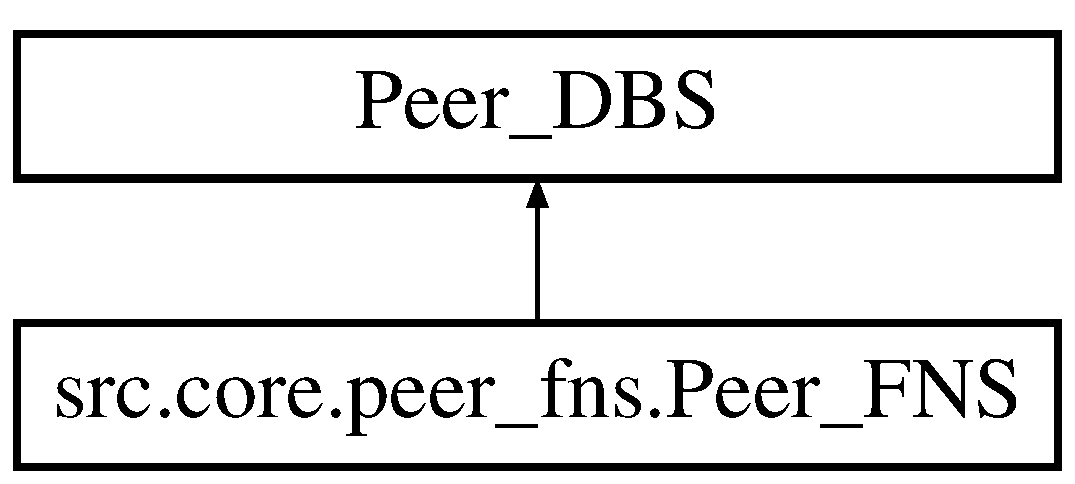
\includegraphics[height=2.000000cm]{classsrc_1_1core_1_1peer__fns_1_1Peer__FNS}
\end{center}
\end{figure}
\subsection*{Public Member Functions}
\begin{DoxyCompactItemize}
\item 
def \hyperlink{classsrc_1_1core_1_1peer__fns_1_1Peer__FNS_add62365f0e76e237a2afea266d6d8e9f}{\+\_\+\+\_\+init\+\_\+\+\_\+} (self, peer)
\item 
def \hyperlink{classsrc_1_1core_1_1peer__fns_1_1Peer__FNS_a2410af318363868b00f0f8fa18f397a7}{say\+\_\+hello} (self, node)
\item 
def \hyperlink{classsrc_1_1core_1_1peer__fns_1_1Peer__FNS_ae515a024ecc249ab904593624193fa96}{say\+\_\+goodbye} (self, node)
\item 
def \hyperlink{classsrc_1_1core_1_1peer__fns_1_1Peer__FNS_a951e42dc0a6f4be5c1af68556be798f7}{disconnect\+\_\+from\+\_\+the\+\_\+splitter} (self)
\end{DoxyCompactItemize}
\subsection*{Public Attributes}
\begin{DoxyCompactItemize}
\item 
\hyperlink{classsrc_1_1core_1_1peer__fns_1_1Peer__FNS_a64da3201be6d30b32b753aebe3912f2a}{splitter\+\_\+socket}
\item 
\hyperlink{classsrc_1_1core_1_1peer__fns_1_1Peer__FNS_a343d7e16e297d587b98aea610d78c9a0}{player\+\_\+socket}
\item 
\hyperlink{classsrc_1_1core_1_1peer__fns_1_1Peer__FNS_aeb76bf05631dc0328b187fbe8b515787}{buffer\+\_\+size}
\item 
\hyperlink{classsrc_1_1core_1_1peer__fns_1_1Peer__FNS_a805fbda31ea75f27a7e199233386bfb8}{splitter}
\item 
\hyperlink{classsrc_1_1core_1_1peer__fns_1_1Peer__FNS_a51c014b49148839d4574f68c5a645a6a}{chunk\+\_\+size}
\item 
\hyperlink{classsrc_1_1core_1_1peer__fns_1_1Peer__FNS_ac2b317a2c4554a289b511e3e0c974627}{peer\+\_\+list}
\item 
\hyperlink{classsrc_1_1core_1_1peer__fns_1_1Peer__FNS_a15de503ef4cf39395f5382b64892d64c}{debt}
\item 
\hyperlink{classsrc_1_1core_1_1peer__fns_1_1Peer__FNS_aabecbc30c2e1c611eb30ef01f7d60477}{message\+\_\+format}
\item 
\hyperlink{classsrc_1_1core_1_1peer__fns_1_1Peer__FNS_a3719c51b8e616b9d2ad093d9a3543e26}{team\+\_\+socket}
\end{DoxyCompactItemize}


\subsection{Constructor \& Destructor Documentation}
\hypertarget{classsrc_1_1core_1_1peer__fns_1_1Peer__FNS_add62365f0e76e237a2afea266d6d8e9f}{}\index{src\+::core\+::peer\+\_\+fns\+::\+Peer\+\_\+\+F\+N\+S@{src\+::core\+::peer\+\_\+fns\+::\+Peer\+\_\+\+F\+N\+S}!\+\_\+\+\_\+init\+\_\+\+\_\+@{\+\_\+\+\_\+init\+\_\+\+\_\+}}
\index{\+\_\+\+\_\+init\+\_\+\+\_\+@{\+\_\+\+\_\+init\+\_\+\+\_\+}!src\+::core\+::peer\+\_\+fns\+::\+Peer\+\_\+\+F\+N\+S@{src\+::core\+::peer\+\_\+fns\+::\+Peer\+\_\+\+F\+N\+S}}
\subsubsection[{\+\_\+\+\_\+init\+\_\+\+\_\+}]{\setlength{\rightskip}{0pt plus 5cm}def src.\+core.\+peer\+\_\+fns.\+Peer\+\_\+\+F\+N\+S.\+\_\+\+\_\+init\+\_\+\+\_\+ (
\begin{DoxyParamCaption}
\item[{}]{self, }
\item[{}]{peer}
\end{DoxyParamCaption}
)}\label{classsrc_1_1core_1_1peer__fns_1_1Peer__FNS_add62365f0e76e237a2afea266d6d8e9f}


\subsection{Member Function Documentation}
\hypertarget{classsrc_1_1core_1_1peer__fns_1_1Peer__FNS_a951e42dc0a6f4be5c1af68556be798f7}{}\index{src\+::core\+::peer\+\_\+fns\+::\+Peer\+\_\+\+F\+N\+S@{src\+::core\+::peer\+\_\+fns\+::\+Peer\+\_\+\+F\+N\+S}!disconnect\+\_\+from\+\_\+the\+\_\+splitter@{disconnect\+\_\+from\+\_\+the\+\_\+splitter}}
\index{disconnect\+\_\+from\+\_\+the\+\_\+splitter@{disconnect\+\_\+from\+\_\+the\+\_\+splitter}!src\+::core\+::peer\+\_\+fns\+::\+Peer\+\_\+\+F\+N\+S@{src\+::core\+::peer\+\_\+fns\+::\+Peer\+\_\+\+F\+N\+S}}
\subsubsection[{disconnect\+\_\+from\+\_\+the\+\_\+splitter}]{\setlength{\rightskip}{0pt plus 5cm}def src.\+core.\+peer\+\_\+fns.\+Peer\+\_\+\+F\+N\+S.\+disconnect\+\_\+from\+\_\+the\+\_\+splitter (
\begin{DoxyParamCaption}
\item[{}]{self}
\end{DoxyParamCaption}
)}\label{classsrc_1_1core_1_1peer__fns_1_1Peer__FNS_a951e42dc0a6f4be5c1af68556be798f7}
\hypertarget{classsrc_1_1core_1_1peer__fns_1_1Peer__FNS_ae515a024ecc249ab904593624193fa96}{}\index{src\+::core\+::peer\+\_\+fns\+::\+Peer\+\_\+\+F\+N\+S@{src\+::core\+::peer\+\_\+fns\+::\+Peer\+\_\+\+F\+N\+S}!say\+\_\+goodbye@{say\+\_\+goodbye}}
\index{say\+\_\+goodbye@{say\+\_\+goodbye}!src\+::core\+::peer\+\_\+fns\+::\+Peer\+\_\+\+F\+N\+S@{src\+::core\+::peer\+\_\+fns\+::\+Peer\+\_\+\+F\+N\+S}}
\subsubsection[{say\+\_\+goodbye}]{\setlength{\rightskip}{0pt plus 5cm}def src.\+core.\+peer\+\_\+fns.\+Peer\+\_\+\+F\+N\+S.\+say\+\_\+goodbye (
\begin{DoxyParamCaption}
\item[{}]{self, }
\item[{}]{node}
\end{DoxyParamCaption}
)}\label{classsrc_1_1core_1_1peer__fns_1_1Peer__FNS_ae515a024ecc249ab904593624193fa96}
\hypertarget{classsrc_1_1core_1_1peer__fns_1_1Peer__FNS_a2410af318363868b00f0f8fa18f397a7}{}\index{src\+::core\+::peer\+\_\+fns\+::\+Peer\+\_\+\+F\+N\+S@{src\+::core\+::peer\+\_\+fns\+::\+Peer\+\_\+\+F\+N\+S}!say\+\_\+hello@{say\+\_\+hello}}
\index{say\+\_\+hello@{say\+\_\+hello}!src\+::core\+::peer\+\_\+fns\+::\+Peer\+\_\+\+F\+N\+S@{src\+::core\+::peer\+\_\+fns\+::\+Peer\+\_\+\+F\+N\+S}}
\subsubsection[{say\+\_\+hello}]{\setlength{\rightskip}{0pt plus 5cm}def src.\+core.\+peer\+\_\+fns.\+Peer\+\_\+\+F\+N\+S.\+say\+\_\+hello (
\begin{DoxyParamCaption}
\item[{}]{self, }
\item[{}]{node}
\end{DoxyParamCaption}
)}\label{classsrc_1_1core_1_1peer__fns_1_1Peer__FNS_a2410af318363868b00f0f8fa18f397a7}


\subsection{Member Data Documentation}
\hypertarget{classsrc_1_1core_1_1peer__fns_1_1Peer__FNS_aeb76bf05631dc0328b187fbe8b515787}{}\index{src\+::core\+::peer\+\_\+fns\+::\+Peer\+\_\+\+F\+N\+S@{src\+::core\+::peer\+\_\+fns\+::\+Peer\+\_\+\+F\+N\+S}!buffer\+\_\+size@{buffer\+\_\+size}}
\index{buffer\+\_\+size@{buffer\+\_\+size}!src\+::core\+::peer\+\_\+fns\+::\+Peer\+\_\+\+F\+N\+S@{src\+::core\+::peer\+\_\+fns\+::\+Peer\+\_\+\+F\+N\+S}}
\subsubsection[{buffer\+\_\+size}]{\setlength{\rightskip}{0pt plus 5cm}src.\+core.\+peer\+\_\+fns.\+Peer\+\_\+\+F\+N\+S.\+buffer\+\_\+size}\label{classsrc_1_1core_1_1peer__fns_1_1Peer__FNS_aeb76bf05631dc0328b187fbe8b515787}
\hypertarget{classsrc_1_1core_1_1peer__fns_1_1Peer__FNS_a51c014b49148839d4574f68c5a645a6a}{}\index{src\+::core\+::peer\+\_\+fns\+::\+Peer\+\_\+\+F\+N\+S@{src\+::core\+::peer\+\_\+fns\+::\+Peer\+\_\+\+F\+N\+S}!chunk\+\_\+size@{chunk\+\_\+size}}
\index{chunk\+\_\+size@{chunk\+\_\+size}!src\+::core\+::peer\+\_\+fns\+::\+Peer\+\_\+\+F\+N\+S@{src\+::core\+::peer\+\_\+fns\+::\+Peer\+\_\+\+F\+N\+S}}
\subsubsection[{chunk\+\_\+size}]{\setlength{\rightskip}{0pt plus 5cm}src.\+core.\+peer\+\_\+fns.\+Peer\+\_\+\+F\+N\+S.\+chunk\+\_\+size}\label{classsrc_1_1core_1_1peer__fns_1_1Peer__FNS_a51c014b49148839d4574f68c5a645a6a}
\hypertarget{classsrc_1_1core_1_1peer__fns_1_1Peer__FNS_a15de503ef4cf39395f5382b64892d64c}{}\index{src\+::core\+::peer\+\_\+fns\+::\+Peer\+\_\+\+F\+N\+S@{src\+::core\+::peer\+\_\+fns\+::\+Peer\+\_\+\+F\+N\+S}!debt@{debt}}
\index{debt@{debt}!src\+::core\+::peer\+\_\+fns\+::\+Peer\+\_\+\+F\+N\+S@{src\+::core\+::peer\+\_\+fns\+::\+Peer\+\_\+\+F\+N\+S}}
\subsubsection[{debt}]{\setlength{\rightskip}{0pt plus 5cm}src.\+core.\+peer\+\_\+fns.\+Peer\+\_\+\+F\+N\+S.\+debt}\label{classsrc_1_1core_1_1peer__fns_1_1Peer__FNS_a15de503ef4cf39395f5382b64892d64c}
\hypertarget{classsrc_1_1core_1_1peer__fns_1_1Peer__FNS_aabecbc30c2e1c611eb30ef01f7d60477}{}\index{src\+::core\+::peer\+\_\+fns\+::\+Peer\+\_\+\+F\+N\+S@{src\+::core\+::peer\+\_\+fns\+::\+Peer\+\_\+\+F\+N\+S}!message\+\_\+format@{message\+\_\+format}}
\index{message\+\_\+format@{message\+\_\+format}!src\+::core\+::peer\+\_\+fns\+::\+Peer\+\_\+\+F\+N\+S@{src\+::core\+::peer\+\_\+fns\+::\+Peer\+\_\+\+F\+N\+S}}
\subsubsection[{message\+\_\+format}]{\setlength{\rightskip}{0pt plus 5cm}src.\+core.\+peer\+\_\+fns.\+Peer\+\_\+\+F\+N\+S.\+message\+\_\+format}\label{classsrc_1_1core_1_1peer__fns_1_1Peer__FNS_aabecbc30c2e1c611eb30ef01f7d60477}
\hypertarget{classsrc_1_1core_1_1peer__fns_1_1Peer__FNS_ac2b317a2c4554a289b511e3e0c974627}{}\index{src\+::core\+::peer\+\_\+fns\+::\+Peer\+\_\+\+F\+N\+S@{src\+::core\+::peer\+\_\+fns\+::\+Peer\+\_\+\+F\+N\+S}!peer\+\_\+list@{peer\+\_\+list}}
\index{peer\+\_\+list@{peer\+\_\+list}!src\+::core\+::peer\+\_\+fns\+::\+Peer\+\_\+\+F\+N\+S@{src\+::core\+::peer\+\_\+fns\+::\+Peer\+\_\+\+F\+N\+S}}
\subsubsection[{peer\+\_\+list}]{\setlength{\rightskip}{0pt plus 5cm}src.\+core.\+peer\+\_\+fns.\+Peer\+\_\+\+F\+N\+S.\+peer\+\_\+list}\label{classsrc_1_1core_1_1peer__fns_1_1Peer__FNS_ac2b317a2c4554a289b511e3e0c974627}
\hypertarget{classsrc_1_1core_1_1peer__fns_1_1Peer__FNS_a343d7e16e297d587b98aea610d78c9a0}{}\index{src\+::core\+::peer\+\_\+fns\+::\+Peer\+\_\+\+F\+N\+S@{src\+::core\+::peer\+\_\+fns\+::\+Peer\+\_\+\+F\+N\+S}!player\+\_\+socket@{player\+\_\+socket}}
\index{player\+\_\+socket@{player\+\_\+socket}!src\+::core\+::peer\+\_\+fns\+::\+Peer\+\_\+\+F\+N\+S@{src\+::core\+::peer\+\_\+fns\+::\+Peer\+\_\+\+F\+N\+S}}
\subsubsection[{player\+\_\+socket}]{\setlength{\rightskip}{0pt plus 5cm}src.\+core.\+peer\+\_\+fns.\+Peer\+\_\+\+F\+N\+S.\+player\+\_\+socket}\label{classsrc_1_1core_1_1peer__fns_1_1Peer__FNS_a343d7e16e297d587b98aea610d78c9a0}
\hypertarget{classsrc_1_1core_1_1peer__fns_1_1Peer__FNS_a805fbda31ea75f27a7e199233386bfb8}{}\index{src\+::core\+::peer\+\_\+fns\+::\+Peer\+\_\+\+F\+N\+S@{src\+::core\+::peer\+\_\+fns\+::\+Peer\+\_\+\+F\+N\+S}!splitter@{splitter}}
\index{splitter@{splitter}!src\+::core\+::peer\+\_\+fns\+::\+Peer\+\_\+\+F\+N\+S@{src\+::core\+::peer\+\_\+fns\+::\+Peer\+\_\+\+F\+N\+S}}
\subsubsection[{splitter}]{\setlength{\rightskip}{0pt plus 5cm}src.\+core.\+peer\+\_\+fns.\+Peer\+\_\+\+F\+N\+S.\+splitter}\label{classsrc_1_1core_1_1peer__fns_1_1Peer__FNS_a805fbda31ea75f27a7e199233386bfb8}
\hypertarget{classsrc_1_1core_1_1peer__fns_1_1Peer__FNS_a64da3201be6d30b32b753aebe3912f2a}{}\index{src\+::core\+::peer\+\_\+fns\+::\+Peer\+\_\+\+F\+N\+S@{src\+::core\+::peer\+\_\+fns\+::\+Peer\+\_\+\+F\+N\+S}!splitter\+\_\+socket@{splitter\+\_\+socket}}
\index{splitter\+\_\+socket@{splitter\+\_\+socket}!src\+::core\+::peer\+\_\+fns\+::\+Peer\+\_\+\+F\+N\+S@{src\+::core\+::peer\+\_\+fns\+::\+Peer\+\_\+\+F\+N\+S}}
\subsubsection[{splitter\+\_\+socket}]{\setlength{\rightskip}{0pt plus 5cm}src.\+core.\+peer\+\_\+fns.\+Peer\+\_\+\+F\+N\+S.\+splitter\+\_\+socket}\label{classsrc_1_1core_1_1peer__fns_1_1Peer__FNS_a64da3201be6d30b32b753aebe3912f2a}
\hypertarget{classsrc_1_1core_1_1peer__fns_1_1Peer__FNS_a3719c51b8e616b9d2ad093d9a3543e26}{}\index{src\+::core\+::peer\+\_\+fns\+::\+Peer\+\_\+\+F\+N\+S@{src\+::core\+::peer\+\_\+fns\+::\+Peer\+\_\+\+F\+N\+S}!team\+\_\+socket@{team\+\_\+socket}}
\index{team\+\_\+socket@{team\+\_\+socket}!src\+::core\+::peer\+\_\+fns\+::\+Peer\+\_\+\+F\+N\+S@{src\+::core\+::peer\+\_\+fns\+::\+Peer\+\_\+\+F\+N\+S}}
\subsubsection[{team\+\_\+socket}]{\setlength{\rightskip}{0pt plus 5cm}src.\+core.\+peer\+\_\+fns.\+Peer\+\_\+\+F\+N\+S.\+team\+\_\+socket}\label{classsrc_1_1core_1_1peer__fns_1_1Peer__FNS_a3719c51b8e616b9d2ad093d9a3543e26}


The documentation for this class was generated from the following file\+:\begin{DoxyCompactItemize}
\item 
src/core/\hyperlink{peer__fns_8py}{peer\+\_\+fns.\+py}\end{DoxyCompactItemize}

\hypertarget{classsrc_1_1core_1_1peer__ims_1_1Peer__IMS}{}\section{src.\+core.\+peer\+\_\+ims.\+Peer\+\_\+\+I\+M\+S Class Reference}
\label{classsrc_1_1core_1_1peer__ims_1_1Peer__IMS}\index{src.\+core.\+peer\+\_\+ims.\+Peer\+\_\+\+I\+M\+S@{src.\+core.\+peer\+\_\+ims.\+Peer\+\_\+\+I\+M\+S}}
Inheritance diagram for src.\+core.\+peer\+\_\+ims.\+Peer\+\_\+\+I\+M\+S\+:\begin{figure}[H]
\begin{center}
\leavevmode
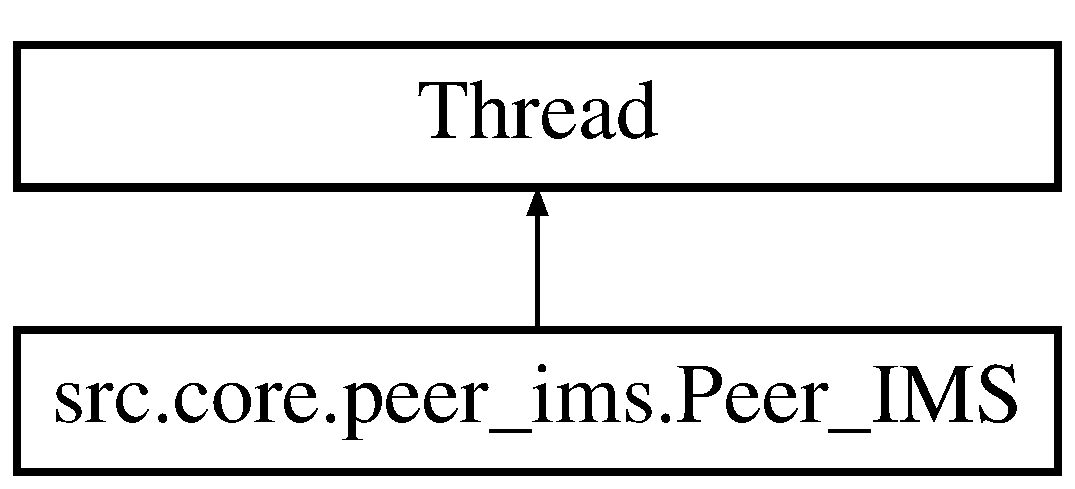
\includegraphics[height=2.000000cm]{classsrc_1_1core_1_1peer__ims_1_1Peer__IMS}
\end{center}
\end{figure}
\subsection*{Public Member Functions}
\begin{DoxyCompactItemize}
\item 
def \hyperlink{classsrc_1_1core_1_1peer__ims_1_1Peer__IMS_a525c10b59682da32a7502314bd4b1f5e}{\+\_\+\+\_\+init\+\_\+\+\_\+} (self)
\item 
def \hyperlink{classsrc_1_1core_1_1peer__ims_1_1Peer__IMS_ab8ab41fb26aaa0d44235a5a7dfcba6b5}{wait\+\_\+for\+\_\+the\+\_\+player} (self)
\item 
def \hyperlink{classsrc_1_1core_1_1peer__ims_1_1Peer__IMS_a2071b641d1a934130e33f6de44e23a2d}{connect\+\_\+to\+\_\+the\+\_\+splitter} (self)
\item 
def \hyperlink{classsrc_1_1core_1_1peer__ims_1_1Peer__IMS_a27d57f696759788043cc6b166fc13855}{disconnect\+\_\+from\+\_\+the\+\_\+splitter} (self)
\item 
def \hyperlink{classsrc_1_1core_1_1peer__ims_1_1Peer__IMS_a4351f780525246f64f8d18d494ccbd8d}{receive\+\_\+the\+\_\+mcast\+\_\+endpoint} (self)
\item 
def \hyperlink{classsrc_1_1core_1_1peer__ims_1_1Peer__IMS_a0880486948cf97e67fff032e93f54f32}{receive\+\_\+the\+\_\+header} (self)
\item 
def \hyperlink{classsrc_1_1core_1_1peer__ims_1_1Peer__IMS_a3e1d60b49169056d27193917740dc625}{receive\+\_\+the\+\_\+chunk\+\_\+size} (self)
\item 
def \hyperlink{classsrc_1_1core_1_1peer__ims_1_1Peer__IMS_ae7993f21d5127ea020cebc00e95012de}{receive\+\_\+the\+\_\+header\+\_\+size} (self)
\item 
def \hyperlink{classsrc_1_1core_1_1peer__ims_1_1Peer__IMS_aa3778cc26a31a96f7624466c855edcbb}{receive\+\_\+the\+\_\+buffer\+\_\+size} (self)
\item 
def \hyperlink{classsrc_1_1core_1_1peer__ims_1_1Peer__IMS_a701dfdceeb9b0eeb56b9fb42176e8e39}{listen\+\_\+to\+\_\+the\+\_\+team} (self)
\item 
def \hyperlink{classsrc_1_1core_1_1peer__ims_1_1Peer__IMS_a117a1ce826a5599d5bd2c365de57d240}{unpack\+\_\+message} (self, message)
\item 
def \hyperlink{classsrc_1_1core_1_1peer__ims_1_1Peer__IMS_a8102399ab64bde214354188129bf92e9}{receive\+\_\+the\+\_\+next\+\_\+message} (self)
\item 
def \hyperlink{classsrc_1_1core_1_1peer__ims_1_1Peer__IMS_a85dc71bbe56d2d543c700733a4603ce0}{process\+\_\+next\+\_\+message} (self)
\item 
def \hyperlink{classsrc_1_1core_1_1peer__ims_1_1Peer__IMS_a16ac77236618eefed91bccef8fa649b7}{buffer\+\_\+data} (self)
\item 
def \hyperlink{classsrc_1_1core_1_1peer__ims_1_1Peer__IMS_af7333f1126e87bf75e3a78c008b83097}{find\+\_\+next\+\_\+chunk} (self)
\item 
def \hyperlink{classsrc_1_1core_1_1peer__ims_1_1Peer__IMS_a18fc8211a694d8f4a827a2d9f5d17cae}{play\+\_\+chunk} (self, chunk)
\item 
def \hyperlink{classsrc_1_1core_1_1peer__ims_1_1Peer__IMS_a02867aca9091f129e3dea02e2c3fbff3}{play\+\_\+next\+\_\+chunk} (self)
\item 
def \hyperlink{classsrc_1_1core_1_1peer__ims_1_1Peer__IMS_a3dc2428cf6b96abfcda36b2e99a692bc}{play} (self)
\item 
def \hyperlink{classsrc_1_1core_1_1peer__ims_1_1Peer__IMS_a3ddd592cf7eafecde6cf83815295b84b}{keep\+\_\+the\+\_\+buffer\+\_\+full} (self)
\begin{DoxyCompactList}\small\item\em def receive\+\_\+configuration(self)\+: \subsection*{\{\{\{}\end{DoxyCompactList}\item 
def \hyperlink{classsrc_1_1core_1_1peer__ims_1_1Peer__IMS_a257ba1bbcfc1f440ca0df28b04b9be4f}{run} (self)
\end{DoxyCompactItemize}
\subsection*{Public Attributes}
\begin{DoxyCompactItemize}
\item 
\hyperlink{classsrc_1_1core_1_1peer__ims_1_1Peer__IMS_af0cec94f2c4e2d2a8e99c748fb9fa5b5}{player\+\_\+socket}
\item 
\hyperlink{classsrc_1_1core_1_1peer__ims_1_1Peer__IMS_a2b943b00f57f4bb49e0f41dfbf6a0cda}{splitter\+\_\+socket}
\item 
\hyperlink{classsrc_1_1core_1_1peer__ims_1_1Peer__IMS_ad7cecf51b6f701abb603443b2f9e36b1}{splitter}
\item 
\hyperlink{classsrc_1_1core_1_1peer__ims_1_1Peer__IMS_a92b3ec069f40b71ae5ca3d394e17601c}{mcast\+\_\+addr}
\item 
\hyperlink{classsrc_1_1core_1_1peer__ims_1_1Peer__IMS_a1ce7993dc45129cfac9bfad943b66b50}{mcast\+\_\+port}
\item 
\hyperlink{classsrc_1_1core_1_1peer__ims_1_1Peer__IMS_a5f010bb5b156212027865fedc8628905}{chunk\+\_\+size}
\item 
\hyperlink{classsrc_1_1core_1_1peer__ims_1_1Peer__IMS_af146f20975eb7b1b089c0746210fbf4f}{message\+\_\+format}
\item 
\hyperlink{classsrc_1_1core_1_1peer__ims_1_1Peer__IMS_a066851fd6c8bf052bff059f91231a32e}{header\+\_\+size\+\_\+in\+\_\+chunks}
\item 
\hyperlink{classsrc_1_1core_1_1peer__ims_1_1Peer__IMS_a1a05d80c5b6b7337394fe3cd747027a9}{buffer\+\_\+size}
\item 
\hyperlink{classsrc_1_1core_1_1peer__ims_1_1Peer__IMS_a8168fae98550467966429b742e9fda58}{team\+\_\+socket}
\item 
\hyperlink{classsrc_1_1core_1_1peer__ims_1_1Peer__IMS_acebb1381bd1a801a8f2bf99f9757ee59}{player\+\_\+alive}
\item 
\hyperlink{classsrc_1_1core_1_1peer__ims_1_1Peer__IMS_ab226eb6bed3d6d26a36ec331ae6ea7e7}{played\+\_\+chunk}
\item 
\hyperlink{classsrc_1_1core_1_1peer__ims_1_1Peer__IMS_a8e39550d083eead799143f49ae2d083c}{recvfrom\+\_\+counter}
\item 
\hyperlink{classsrc_1_1core_1_1peer__ims_1_1Peer__IMS_a8fea5fe4e14a4ab2afb3673a04faffa5}{received\+\_\+flag}
\item 
\hyperlink{classsrc_1_1core_1_1peer__ims_1_1Peer__IMS_adf33b563fd6d50f0d86bbd87797405ce}{chunks}
\item 
\hyperlink{classsrc_1_1core_1_1peer__ims_1_1Peer__IMS_a44374641cdc36487318e7ab38e052892}{received\+\_\+counter}
\end{DoxyCompactItemize}
\subsection*{Static Public Attributes}
\begin{DoxyCompactItemize}
\item 
int \hyperlink{classsrc_1_1core_1_1peer__ims_1_1Peer__IMS_a7d5fe41966aac3f32e79e50775247732}{P\+L\+A\+Y\+E\+R\+\_\+\+P\+O\+R\+T} = 9999
\item 
string \hyperlink{classsrc_1_1core_1_1peer__ims_1_1Peer__IMS_aa3073dc0de163fb99b97eb1f44afa909}{S\+P\+L\+I\+T\+T\+E\+R\+\_\+\+A\+D\+D\+R} = \char`\"{}127.\+0.\+0.\+1\char`\"{}
\item 
int \hyperlink{classsrc_1_1core_1_1peer__ims_1_1Peer__IMS_a2c62c4b734b0e70089b81c87d37a7a71}{S\+P\+L\+I\+T\+T\+E\+R\+\_\+\+P\+O\+R\+T} = 4552
\item 
int \hyperlink{classsrc_1_1core_1_1peer__ims_1_1Peer__IMS_a365247e52d008b94cb47e0ff9bf6e7d8}{P\+O\+R\+T} = 0
\item 
\hyperlink{classsrc_1_1core_1_1peer__ims_1_1Peer__IMS_aca1872083e540265591dd9dc51113f0b}{U\+S\+E\+\_\+\+L\+O\+C\+A\+L\+H\+O\+S\+T} = False
\item 
tuple \hyperlink{classsrc_1_1core_1_1peer__ims_1_1Peer__IMS_ac28a1563f853b5d463453ade44ed0026}{B\+U\+F\+F\+E\+R\+\_\+\+S\+T\+A\+T\+U\+S} = int(0)
\end{DoxyCompactItemize}


\subsection{Constructor \& Destructor Documentation}
\hypertarget{classsrc_1_1core_1_1peer__ims_1_1Peer__IMS_a525c10b59682da32a7502314bd4b1f5e}{}\index{src\+::core\+::peer\+\_\+ims\+::\+Peer\+\_\+\+I\+M\+S@{src\+::core\+::peer\+\_\+ims\+::\+Peer\+\_\+\+I\+M\+S}!\+\_\+\+\_\+init\+\_\+\+\_\+@{\+\_\+\+\_\+init\+\_\+\+\_\+}}
\index{\+\_\+\+\_\+init\+\_\+\+\_\+@{\+\_\+\+\_\+init\+\_\+\+\_\+}!src\+::core\+::peer\+\_\+ims\+::\+Peer\+\_\+\+I\+M\+S@{src\+::core\+::peer\+\_\+ims\+::\+Peer\+\_\+\+I\+M\+S}}
\subsubsection[{\+\_\+\+\_\+init\+\_\+\+\_\+}]{\setlength{\rightskip}{0pt plus 5cm}def src.\+core.\+peer\+\_\+ims.\+Peer\+\_\+\+I\+M\+S.\+\_\+\+\_\+init\+\_\+\+\_\+ (
\begin{DoxyParamCaption}
\item[{}]{self}
\end{DoxyParamCaption}
)}\label{classsrc_1_1core_1_1peer__ims_1_1Peer__IMS_a525c10b59682da32a7502314bd4b1f5e}


\subsection{Member Function Documentation}
\hypertarget{classsrc_1_1core_1_1peer__ims_1_1Peer__IMS_a16ac77236618eefed91bccef8fa649b7}{}\index{src\+::core\+::peer\+\_\+ims\+::\+Peer\+\_\+\+I\+M\+S@{src\+::core\+::peer\+\_\+ims\+::\+Peer\+\_\+\+I\+M\+S}!buffer\+\_\+data@{buffer\+\_\+data}}
\index{buffer\+\_\+data@{buffer\+\_\+data}!src\+::core\+::peer\+\_\+ims\+::\+Peer\+\_\+\+I\+M\+S@{src\+::core\+::peer\+\_\+ims\+::\+Peer\+\_\+\+I\+M\+S}}
\subsubsection[{buffer\+\_\+data}]{\setlength{\rightskip}{0pt plus 5cm}def src.\+core.\+peer\+\_\+ims.\+Peer\+\_\+\+I\+M\+S.\+buffer\+\_\+data (
\begin{DoxyParamCaption}
\item[{}]{self}
\end{DoxyParamCaption}
)}\label{classsrc_1_1core_1_1peer__ims_1_1Peer__IMS_a16ac77236618eefed91bccef8fa649b7}
\hypertarget{classsrc_1_1core_1_1peer__ims_1_1Peer__IMS_a2071b641d1a934130e33f6de44e23a2d}{}\index{src\+::core\+::peer\+\_\+ims\+::\+Peer\+\_\+\+I\+M\+S@{src\+::core\+::peer\+\_\+ims\+::\+Peer\+\_\+\+I\+M\+S}!connect\+\_\+to\+\_\+the\+\_\+splitter@{connect\+\_\+to\+\_\+the\+\_\+splitter}}
\index{connect\+\_\+to\+\_\+the\+\_\+splitter@{connect\+\_\+to\+\_\+the\+\_\+splitter}!src\+::core\+::peer\+\_\+ims\+::\+Peer\+\_\+\+I\+M\+S@{src\+::core\+::peer\+\_\+ims\+::\+Peer\+\_\+\+I\+M\+S}}
\subsubsection[{connect\+\_\+to\+\_\+the\+\_\+splitter}]{\setlength{\rightskip}{0pt plus 5cm}def src.\+core.\+peer\+\_\+ims.\+Peer\+\_\+\+I\+M\+S.\+connect\+\_\+to\+\_\+the\+\_\+splitter (
\begin{DoxyParamCaption}
\item[{}]{self}
\end{DoxyParamCaption}
)}\label{classsrc_1_1core_1_1peer__ims_1_1Peer__IMS_a2071b641d1a934130e33f6de44e23a2d}
\hypertarget{classsrc_1_1core_1_1peer__ims_1_1Peer__IMS_a27d57f696759788043cc6b166fc13855}{}\index{src\+::core\+::peer\+\_\+ims\+::\+Peer\+\_\+\+I\+M\+S@{src\+::core\+::peer\+\_\+ims\+::\+Peer\+\_\+\+I\+M\+S}!disconnect\+\_\+from\+\_\+the\+\_\+splitter@{disconnect\+\_\+from\+\_\+the\+\_\+splitter}}
\index{disconnect\+\_\+from\+\_\+the\+\_\+splitter@{disconnect\+\_\+from\+\_\+the\+\_\+splitter}!src\+::core\+::peer\+\_\+ims\+::\+Peer\+\_\+\+I\+M\+S@{src\+::core\+::peer\+\_\+ims\+::\+Peer\+\_\+\+I\+M\+S}}
\subsubsection[{disconnect\+\_\+from\+\_\+the\+\_\+splitter}]{\setlength{\rightskip}{0pt plus 5cm}def src.\+core.\+peer\+\_\+ims.\+Peer\+\_\+\+I\+M\+S.\+disconnect\+\_\+from\+\_\+the\+\_\+splitter (
\begin{DoxyParamCaption}
\item[{}]{self}
\end{DoxyParamCaption}
)}\label{classsrc_1_1core_1_1peer__ims_1_1Peer__IMS_a27d57f696759788043cc6b166fc13855}
\hypertarget{classsrc_1_1core_1_1peer__ims_1_1Peer__IMS_af7333f1126e87bf75e3a78c008b83097}{}\index{src\+::core\+::peer\+\_\+ims\+::\+Peer\+\_\+\+I\+M\+S@{src\+::core\+::peer\+\_\+ims\+::\+Peer\+\_\+\+I\+M\+S}!find\+\_\+next\+\_\+chunk@{find\+\_\+next\+\_\+chunk}}
\index{find\+\_\+next\+\_\+chunk@{find\+\_\+next\+\_\+chunk}!src\+::core\+::peer\+\_\+ims\+::\+Peer\+\_\+\+I\+M\+S@{src\+::core\+::peer\+\_\+ims\+::\+Peer\+\_\+\+I\+M\+S}}
\subsubsection[{find\+\_\+next\+\_\+chunk}]{\setlength{\rightskip}{0pt plus 5cm}def src.\+core.\+peer\+\_\+ims.\+Peer\+\_\+\+I\+M\+S.\+find\+\_\+next\+\_\+chunk (
\begin{DoxyParamCaption}
\item[{}]{self}
\end{DoxyParamCaption}
)}\label{classsrc_1_1core_1_1peer__ims_1_1Peer__IMS_af7333f1126e87bf75e3a78c008b83097}
\hypertarget{classsrc_1_1core_1_1peer__ims_1_1Peer__IMS_a3ddd592cf7eafecde6cf83815295b84b}{}\index{src\+::core\+::peer\+\_\+ims\+::\+Peer\+\_\+\+I\+M\+S@{src\+::core\+::peer\+\_\+ims\+::\+Peer\+\_\+\+I\+M\+S}!keep\+\_\+the\+\_\+buffer\+\_\+full@{keep\+\_\+the\+\_\+buffer\+\_\+full}}
\index{keep\+\_\+the\+\_\+buffer\+\_\+full@{keep\+\_\+the\+\_\+buffer\+\_\+full}!src\+::core\+::peer\+\_\+ims\+::\+Peer\+\_\+\+I\+M\+S@{src\+::core\+::peer\+\_\+ims\+::\+Peer\+\_\+\+I\+M\+S}}
\subsubsection[{keep\+\_\+the\+\_\+buffer\+\_\+full}]{\setlength{\rightskip}{0pt plus 5cm}def src.\+core.\+peer\+\_\+ims.\+Peer\+\_\+\+I\+M\+S.\+keep\+\_\+the\+\_\+buffer\+\_\+full (
\begin{DoxyParamCaption}
\item[{}]{self}
\end{DoxyParamCaption}
)}\label{classsrc_1_1core_1_1peer__ims_1_1Peer__IMS_a3ddd592cf7eafecde6cf83815295b84b}


def receive\+\_\+configuration(self)\+: \subsection*{\{\{\{}

self.\+receive\+\_\+the\+\_\+mcast\+\_\+endpoint() self.\+receive\+\_\+the\+\_\+header\+\_\+size() self.\+receive\+\_\+the\+\_\+chunk\+\_\+size() self.\+receive\+\_\+the\+\_\+header() self.\+receive\+\_\+the\+\_\+buffer\+\_\+size() \# \}\}\} \hypertarget{classsrc_1_1core_1_1peer__ims_1_1Peer__IMS_a701dfdceeb9b0eeb56b9fb42176e8e39}{}\index{src\+::core\+::peer\+\_\+ims\+::\+Peer\+\_\+\+I\+M\+S@{src\+::core\+::peer\+\_\+ims\+::\+Peer\+\_\+\+I\+M\+S}!listen\+\_\+to\+\_\+the\+\_\+team@{listen\+\_\+to\+\_\+the\+\_\+team}}
\index{listen\+\_\+to\+\_\+the\+\_\+team@{listen\+\_\+to\+\_\+the\+\_\+team}!src\+::core\+::peer\+\_\+ims\+::\+Peer\+\_\+\+I\+M\+S@{src\+::core\+::peer\+\_\+ims\+::\+Peer\+\_\+\+I\+M\+S}}
\subsubsection[{listen\+\_\+to\+\_\+the\+\_\+team}]{\setlength{\rightskip}{0pt plus 5cm}def src.\+core.\+peer\+\_\+ims.\+Peer\+\_\+\+I\+M\+S.\+listen\+\_\+to\+\_\+the\+\_\+team (
\begin{DoxyParamCaption}
\item[{}]{self}
\end{DoxyParamCaption}
)}\label{classsrc_1_1core_1_1peer__ims_1_1Peer__IMS_a701dfdceeb9b0eeb56b9fb42176e8e39}
\hypertarget{classsrc_1_1core_1_1peer__ims_1_1Peer__IMS_a3dc2428cf6b96abfcda36b2e99a692bc}{}\index{src\+::core\+::peer\+\_\+ims\+::\+Peer\+\_\+\+I\+M\+S@{src\+::core\+::peer\+\_\+ims\+::\+Peer\+\_\+\+I\+M\+S}!play@{play}}
\index{play@{play}!src\+::core\+::peer\+\_\+ims\+::\+Peer\+\_\+\+I\+M\+S@{src\+::core\+::peer\+\_\+ims\+::\+Peer\+\_\+\+I\+M\+S}}
\subsubsection[{play}]{\setlength{\rightskip}{0pt plus 5cm}def src.\+core.\+peer\+\_\+ims.\+Peer\+\_\+\+I\+M\+S.\+play (
\begin{DoxyParamCaption}
\item[{}]{self}
\end{DoxyParamCaption}
)}\label{classsrc_1_1core_1_1peer__ims_1_1Peer__IMS_a3dc2428cf6b96abfcda36b2e99a692bc}
\hypertarget{classsrc_1_1core_1_1peer__ims_1_1Peer__IMS_a18fc8211a694d8f4a827a2d9f5d17cae}{}\index{src\+::core\+::peer\+\_\+ims\+::\+Peer\+\_\+\+I\+M\+S@{src\+::core\+::peer\+\_\+ims\+::\+Peer\+\_\+\+I\+M\+S}!play\+\_\+chunk@{play\+\_\+chunk}}
\index{play\+\_\+chunk@{play\+\_\+chunk}!src\+::core\+::peer\+\_\+ims\+::\+Peer\+\_\+\+I\+M\+S@{src\+::core\+::peer\+\_\+ims\+::\+Peer\+\_\+\+I\+M\+S}}
\subsubsection[{play\+\_\+chunk}]{\setlength{\rightskip}{0pt plus 5cm}def src.\+core.\+peer\+\_\+ims.\+Peer\+\_\+\+I\+M\+S.\+play\+\_\+chunk (
\begin{DoxyParamCaption}
\item[{}]{self, }
\item[{}]{chunk}
\end{DoxyParamCaption}
)}\label{classsrc_1_1core_1_1peer__ims_1_1Peer__IMS_a18fc8211a694d8f4a827a2d9f5d17cae}
\hypertarget{classsrc_1_1core_1_1peer__ims_1_1Peer__IMS_a02867aca9091f129e3dea02e2c3fbff3}{}\index{src\+::core\+::peer\+\_\+ims\+::\+Peer\+\_\+\+I\+M\+S@{src\+::core\+::peer\+\_\+ims\+::\+Peer\+\_\+\+I\+M\+S}!play\+\_\+next\+\_\+chunk@{play\+\_\+next\+\_\+chunk}}
\index{play\+\_\+next\+\_\+chunk@{play\+\_\+next\+\_\+chunk}!src\+::core\+::peer\+\_\+ims\+::\+Peer\+\_\+\+I\+M\+S@{src\+::core\+::peer\+\_\+ims\+::\+Peer\+\_\+\+I\+M\+S}}
\subsubsection[{play\+\_\+next\+\_\+chunk}]{\setlength{\rightskip}{0pt plus 5cm}def src.\+core.\+peer\+\_\+ims.\+Peer\+\_\+\+I\+M\+S.\+play\+\_\+next\+\_\+chunk (
\begin{DoxyParamCaption}
\item[{}]{self}
\end{DoxyParamCaption}
)}\label{classsrc_1_1core_1_1peer__ims_1_1Peer__IMS_a02867aca9091f129e3dea02e2c3fbff3}
\hypertarget{classsrc_1_1core_1_1peer__ims_1_1Peer__IMS_a85dc71bbe56d2d543c700733a4603ce0}{}\index{src\+::core\+::peer\+\_\+ims\+::\+Peer\+\_\+\+I\+M\+S@{src\+::core\+::peer\+\_\+ims\+::\+Peer\+\_\+\+I\+M\+S}!process\+\_\+next\+\_\+message@{process\+\_\+next\+\_\+message}}
\index{process\+\_\+next\+\_\+message@{process\+\_\+next\+\_\+message}!src\+::core\+::peer\+\_\+ims\+::\+Peer\+\_\+\+I\+M\+S@{src\+::core\+::peer\+\_\+ims\+::\+Peer\+\_\+\+I\+M\+S}}
\subsubsection[{process\+\_\+next\+\_\+message}]{\setlength{\rightskip}{0pt plus 5cm}def src.\+core.\+peer\+\_\+ims.\+Peer\+\_\+\+I\+M\+S.\+process\+\_\+next\+\_\+message (
\begin{DoxyParamCaption}
\item[{}]{self}
\end{DoxyParamCaption}
)}\label{classsrc_1_1core_1_1peer__ims_1_1Peer__IMS_a85dc71bbe56d2d543c700733a4603ce0}
\hypertarget{classsrc_1_1core_1_1peer__ims_1_1Peer__IMS_aa3778cc26a31a96f7624466c855edcbb}{}\index{src\+::core\+::peer\+\_\+ims\+::\+Peer\+\_\+\+I\+M\+S@{src\+::core\+::peer\+\_\+ims\+::\+Peer\+\_\+\+I\+M\+S}!receive\+\_\+the\+\_\+buffer\+\_\+size@{receive\+\_\+the\+\_\+buffer\+\_\+size}}
\index{receive\+\_\+the\+\_\+buffer\+\_\+size@{receive\+\_\+the\+\_\+buffer\+\_\+size}!src\+::core\+::peer\+\_\+ims\+::\+Peer\+\_\+\+I\+M\+S@{src\+::core\+::peer\+\_\+ims\+::\+Peer\+\_\+\+I\+M\+S}}
\subsubsection[{receive\+\_\+the\+\_\+buffer\+\_\+size}]{\setlength{\rightskip}{0pt plus 5cm}def src.\+core.\+peer\+\_\+ims.\+Peer\+\_\+\+I\+M\+S.\+receive\+\_\+the\+\_\+buffer\+\_\+size (
\begin{DoxyParamCaption}
\item[{}]{self}
\end{DoxyParamCaption}
)}\label{classsrc_1_1core_1_1peer__ims_1_1Peer__IMS_aa3778cc26a31a96f7624466c855edcbb}
\hypertarget{classsrc_1_1core_1_1peer__ims_1_1Peer__IMS_a3e1d60b49169056d27193917740dc625}{}\index{src\+::core\+::peer\+\_\+ims\+::\+Peer\+\_\+\+I\+M\+S@{src\+::core\+::peer\+\_\+ims\+::\+Peer\+\_\+\+I\+M\+S}!receive\+\_\+the\+\_\+chunk\+\_\+size@{receive\+\_\+the\+\_\+chunk\+\_\+size}}
\index{receive\+\_\+the\+\_\+chunk\+\_\+size@{receive\+\_\+the\+\_\+chunk\+\_\+size}!src\+::core\+::peer\+\_\+ims\+::\+Peer\+\_\+\+I\+M\+S@{src\+::core\+::peer\+\_\+ims\+::\+Peer\+\_\+\+I\+M\+S}}
\subsubsection[{receive\+\_\+the\+\_\+chunk\+\_\+size}]{\setlength{\rightskip}{0pt plus 5cm}def src.\+core.\+peer\+\_\+ims.\+Peer\+\_\+\+I\+M\+S.\+receive\+\_\+the\+\_\+chunk\+\_\+size (
\begin{DoxyParamCaption}
\item[{}]{self}
\end{DoxyParamCaption}
)}\label{classsrc_1_1core_1_1peer__ims_1_1Peer__IMS_a3e1d60b49169056d27193917740dc625}
\hypertarget{classsrc_1_1core_1_1peer__ims_1_1Peer__IMS_a0880486948cf97e67fff032e93f54f32}{}\index{src\+::core\+::peer\+\_\+ims\+::\+Peer\+\_\+\+I\+M\+S@{src\+::core\+::peer\+\_\+ims\+::\+Peer\+\_\+\+I\+M\+S}!receive\+\_\+the\+\_\+header@{receive\+\_\+the\+\_\+header}}
\index{receive\+\_\+the\+\_\+header@{receive\+\_\+the\+\_\+header}!src\+::core\+::peer\+\_\+ims\+::\+Peer\+\_\+\+I\+M\+S@{src\+::core\+::peer\+\_\+ims\+::\+Peer\+\_\+\+I\+M\+S}}
\subsubsection[{receive\+\_\+the\+\_\+header}]{\setlength{\rightskip}{0pt plus 5cm}def src.\+core.\+peer\+\_\+ims.\+Peer\+\_\+\+I\+M\+S.\+receive\+\_\+the\+\_\+header (
\begin{DoxyParamCaption}
\item[{}]{self}
\end{DoxyParamCaption}
)}\label{classsrc_1_1core_1_1peer__ims_1_1Peer__IMS_a0880486948cf97e67fff032e93f54f32}
\hypertarget{classsrc_1_1core_1_1peer__ims_1_1Peer__IMS_ae7993f21d5127ea020cebc00e95012de}{}\index{src\+::core\+::peer\+\_\+ims\+::\+Peer\+\_\+\+I\+M\+S@{src\+::core\+::peer\+\_\+ims\+::\+Peer\+\_\+\+I\+M\+S}!receive\+\_\+the\+\_\+header\+\_\+size@{receive\+\_\+the\+\_\+header\+\_\+size}}
\index{receive\+\_\+the\+\_\+header\+\_\+size@{receive\+\_\+the\+\_\+header\+\_\+size}!src\+::core\+::peer\+\_\+ims\+::\+Peer\+\_\+\+I\+M\+S@{src\+::core\+::peer\+\_\+ims\+::\+Peer\+\_\+\+I\+M\+S}}
\subsubsection[{receive\+\_\+the\+\_\+header\+\_\+size}]{\setlength{\rightskip}{0pt plus 5cm}def src.\+core.\+peer\+\_\+ims.\+Peer\+\_\+\+I\+M\+S.\+receive\+\_\+the\+\_\+header\+\_\+size (
\begin{DoxyParamCaption}
\item[{}]{self}
\end{DoxyParamCaption}
)}\label{classsrc_1_1core_1_1peer__ims_1_1Peer__IMS_ae7993f21d5127ea020cebc00e95012de}
\hypertarget{classsrc_1_1core_1_1peer__ims_1_1Peer__IMS_a4351f780525246f64f8d18d494ccbd8d}{}\index{src\+::core\+::peer\+\_\+ims\+::\+Peer\+\_\+\+I\+M\+S@{src\+::core\+::peer\+\_\+ims\+::\+Peer\+\_\+\+I\+M\+S}!receive\+\_\+the\+\_\+mcast\+\_\+endpoint@{receive\+\_\+the\+\_\+mcast\+\_\+endpoint}}
\index{receive\+\_\+the\+\_\+mcast\+\_\+endpoint@{receive\+\_\+the\+\_\+mcast\+\_\+endpoint}!src\+::core\+::peer\+\_\+ims\+::\+Peer\+\_\+\+I\+M\+S@{src\+::core\+::peer\+\_\+ims\+::\+Peer\+\_\+\+I\+M\+S}}
\subsubsection[{receive\+\_\+the\+\_\+mcast\+\_\+endpoint}]{\setlength{\rightskip}{0pt plus 5cm}def src.\+core.\+peer\+\_\+ims.\+Peer\+\_\+\+I\+M\+S.\+receive\+\_\+the\+\_\+mcast\+\_\+endpoint (
\begin{DoxyParamCaption}
\item[{}]{self}
\end{DoxyParamCaption}
)}\label{classsrc_1_1core_1_1peer__ims_1_1Peer__IMS_a4351f780525246f64f8d18d494ccbd8d}
\hypertarget{classsrc_1_1core_1_1peer__ims_1_1Peer__IMS_a8102399ab64bde214354188129bf92e9}{}\index{src\+::core\+::peer\+\_\+ims\+::\+Peer\+\_\+\+I\+M\+S@{src\+::core\+::peer\+\_\+ims\+::\+Peer\+\_\+\+I\+M\+S}!receive\+\_\+the\+\_\+next\+\_\+message@{receive\+\_\+the\+\_\+next\+\_\+message}}
\index{receive\+\_\+the\+\_\+next\+\_\+message@{receive\+\_\+the\+\_\+next\+\_\+message}!src\+::core\+::peer\+\_\+ims\+::\+Peer\+\_\+\+I\+M\+S@{src\+::core\+::peer\+\_\+ims\+::\+Peer\+\_\+\+I\+M\+S}}
\subsubsection[{receive\+\_\+the\+\_\+next\+\_\+message}]{\setlength{\rightskip}{0pt plus 5cm}def src.\+core.\+peer\+\_\+ims.\+Peer\+\_\+\+I\+M\+S.\+receive\+\_\+the\+\_\+next\+\_\+message (
\begin{DoxyParamCaption}
\item[{}]{self}
\end{DoxyParamCaption}
)}\label{classsrc_1_1core_1_1peer__ims_1_1Peer__IMS_a8102399ab64bde214354188129bf92e9}
\hypertarget{classsrc_1_1core_1_1peer__ims_1_1Peer__IMS_a257ba1bbcfc1f440ca0df28b04b9be4f}{}\index{src\+::core\+::peer\+\_\+ims\+::\+Peer\+\_\+\+I\+M\+S@{src\+::core\+::peer\+\_\+ims\+::\+Peer\+\_\+\+I\+M\+S}!run@{run}}
\index{run@{run}!src\+::core\+::peer\+\_\+ims\+::\+Peer\+\_\+\+I\+M\+S@{src\+::core\+::peer\+\_\+ims\+::\+Peer\+\_\+\+I\+M\+S}}
\subsubsection[{run}]{\setlength{\rightskip}{0pt plus 5cm}def src.\+core.\+peer\+\_\+ims.\+Peer\+\_\+\+I\+M\+S.\+run (
\begin{DoxyParamCaption}
\item[{}]{self}
\end{DoxyParamCaption}
)}\label{classsrc_1_1core_1_1peer__ims_1_1Peer__IMS_a257ba1bbcfc1f440ca0df28b04b9be4f}
\hypertarget{classsrc_1_1core_1_1peer__ims_1_1Peer__IMS_a117a1ce826a5599d5bd2c365de57d240}{}\index{src\+::core\+::peer\+\_\+ims\+::\+Peer\+\_\+\+I\+M\+S@{src\+::core\+::peer\+\_\+ims\+::\+Peer\+\_\+\+I\+M\+S}!unpack\+\_\+message@{unpack\+\_\+message}}
\index{unpack\+\_\+message@{unpack\+\_\+message}!src\+::core\+::peer\+\_\+ims\+::\+Peer\+\_\+\+I\+M\+S@{src\+::core\+::peer\+\_\+ims\+::\+Peer\+\_\+\+I\+M\+S}}
\subsubsection[{unpack\+\_\+message}]{\setlength{\rightskip}{0pt plus 5cm}def src.\+core.\+peer\+\_\+ims.\+Peer\+\_\+\+I\+M\+S.\+unpack\+\_\+message (
\begin{DoxyParamCaption}
\item[{}]{self, }
\item[{}]{message}
\end{DoxyParamCaption}
)}\label{classsrc_1_1core_1_1peer__ims_1_1Peer__IMS_a117a1ce826a5599d5bd2c365de57d240}
\hypertarget{classsrc_1_1core_1_1peer__ims_1_1Peer__IMS_ab8ab41fb26aaa0d44235a5a7dfcba6b5}{}\index{src\+::core\+::peer\+\_\+ims\+::\+Peer\+\_\+\+I\+M\+S@{src\+::core\+::peer\+\_\+ims\+::\+Peer\+\_\+\+I\+M\+S}!wait\+\_\+for\+\_\+the\+\_\+player@{wait\+\_\+for\+\_\+the\+\_\+player}}
\index{wait\+\_\+for\+\_\+the\+\_\+player@{wait\+\_\+for\+\_\+the\+\_\+player}!src\+::core\+::peer\+\_\+ims\+::\+Peer\+\_\+\+I\+M\+S@{src\+::core\+::peer\+\_\+ims\+::\+Peer\+\_\+\+I\+M\+S}}
\subsubsection[{wait\+\_\+for\+\_\+the\+\_\+player}]{\setlength{\rightskip}{0pt plus 5cm}def src.\+core.\+peer\+\_\+ims.\+Peer\+\_\+\+I\+M\+S.\+wait\+\_\+for\+\_\+the\+\_\+player (
\begin{DoxyParamCaption}
\item[{}]{self}
\end{DoxyParamCaption}
)}\label{classsrc_1_1core_1_1peer__ims_1_1Peer__IMS_ab8ab41fb26aaa0d44235a5a7dfcba6b5}


\subsection{Member Data Documentation}
\hypertarget{classsrc_1_1core_1_1peer__ims_1_1Peer__IMS_a1a05d80c5b6b7337394fe3cd747027a9}{}\index{src\+::core\+::peer\+\_\+ims\+::\+Peer\+\_\+\+I\+M\+S@{src\+::core\+::peer\+\_\+ims\+::\+Peer\+\_\+\+I\+M\+S}!buffer\+\_\+size@{buffer\+\_\+size}}
\index{buffer\+\_\+size@{buffer\+\_\+size}!src\+::core\+::peer\+\_\+ims\+::\+Peer\+\_\+\+I\+M\+S@{src\+::core\+::peer\+\_\+ims\+::\+Peer\+\_\+\+I\+M\+S}}
\subsubsection[{buffer\+\_\+size}]{\setlength{\rightskip}{0pt plus 5cm}src.\+core.\+peer\+\_\+ims.\+Peer\+\_\+\+I\+M\+S.\+buffer\+\_\+size}\label{classsrc_1_1core_1_1peer__ims_1_1Peer__IMS_a1a05d80c5b6b7337394fe3cd747027a9}
\hypertarget{classsrc_1_1core_1_1peer__ims_1_1Peer__IMS_ac28a1563f853b5d463453ade44ed0026}{}\index{src\+::core\+::peer\+\_\+ims\+::\+Peer\+\_\+\+I\+M\+S@{src\+::core\+::peer\+\_\+ims\+::\+Peer\+\_\+\+I\+M\+S}!B\+U\+F\+F\+E\+R\+\_\+\+S\+T\+A\+T\+U\+S@{B\+U\+F\+F\+E\+R\+\_\+\+S\+T\+A\+T\+U\+S}}
\index{B\+U\+F\+F\+E\+R\+\_\+\+S\+T\+A\+T\+U\+S@{B\+U\+F\+F\+E\+R\+\_\+\+S\+T\+A\+T\+U\+S}!src\+::core\+::peer\+\_\+ims\+::\+Peer\+\_\+\+I\+M\+S@{src\+::core\+::peer\+\_\+ims\+::\+Peer\+\_\+\+I\+M\+S}}
\subsubsection[{B\+U\+F\+F\+E\+R\+\_\+\+S\+T\+A\+T\+U\+S}]{\setlength{\rightskip}{0pt plus 5cm}tuple src.\+core.\+peer\+\_\+ims.\+Peer\+\_\+\+I\+M\+S.\+B\+U\+F\+F\+E\+R\+\_\+\+S\+T\+A\+T\+U\+S = int(0)\hspace{0.3cm}{\ttfamily [static]}}\label{classsrc_1_1core_1_1peer__ims_1_1Peer__IMS_ac28a1563f853b5d463453ade44ed0026}
\hypertarget{classsrc_1_1core_1_1peer__ims_1_1Peer__IMS_a5f010bb5b156212027865fedc8628905}{}\index{src\+::core\+::peer\+\_\+ims\+::\+Peer\+\_\+\+I\+M\+S@{src\+::core\+::peer\+\_\+ims\+::\+Peer\+\_\+\+I\+M\+S}!chunk\+\_\+size@{chunk\+\_\+size}}
\index{chunk\+\_\+size@{chunk\+\_\+size}!src\+::core\+::peer\+\_\+ims\+::\+Peer\+\_\+\+I\+M\+S@{src\+::core\+::peer\+\_\+ims\+::\+Peer\+\_\+\+I\+M\+S}}
\subsubsection[{chunk\+\_\+size}]{\setlength{\rightskip}{0pt plus 5cm}src.\+core.\+peer\+\_\+ims.\+Peer\+\_\+\+I\+M\+S.\+chunk\+\_\+size}\label{classsrc_1_1core_1_1peer__ims_1_1Peer__IMS_a5f010bb5b156212027865fedc8628905}
\hypertarget{classsrc_1_1core_1_1peer__ims_1_1Peer__IMS_adf33b563fd6d50f0d86bbd87797405ce}{}\index{src\+::core\+::peer\+\_\+ims\+::\+Peer\+\_\+\+I\+M\+S@{src\+::core\+::peer\+\_\+ims\+::\+Peer\+\_\+\+I\+M\+S}!chunks@{chunks}}
\index{chunks@{chunks}!src\+::core\+::peer\+\_\+ims\+::\+Peer\+\_\+\+I\+M\+S@{src\+::core\+::peer\+\_\+ims\+::\+Peer\+\_\+\+I\+M\+S}}
\subsubsection[{chunks}]{\setlength{\rightskip}{0pt plus 5cm}src.\+core.\+peer\+\_\+ims.\+Peer\+\_\+\+I\+M\+S.\+chunks}\label{classsrc_1_1core_1_1peer__ims_1_1Peer__IMS_adf33b563fd6d50f0d86bbd87797405ce}
\hypertarget{classsrc_1_1core_1_1peer__ims_1_1Peer__IMS_a066851fd6c8bf052bff059f91231a32e}{}\index{src\+::core\+::peer\+\_\+ims\+::\+Peer\+\_\+\+I\+M\+S@{src\+::core\+::peer\+\_\+ims\+::\+Peer\+\_\+\+I\+M\+S}!header\+\_\+size\+\_\+in\+\_\+chunks@{header\+\_\+size\+\_\+in\+\_\+chunks}}
\index{header\+\_\+size\+\_\+in\+\_\+chunks@{header\+\_\+size\+\_\+in\+\_\+chunks}!src\+::core\+::peer\+\_\+ims\+::\+Peer\+\_\+\+I\+M\+S@{src\+::core\+::peer\+\_\+ims\+::\+Peer\+\_\+\+I\+M\+S}}
\subsubsection[{header\+\_\+size\+\_\+in\+\_\+chunks}]{\setlength{\rightskip}{0pt plus 5cm}src.\+core.\+peer\+\_\+ims.\+Peer\+\_\+\+I\+M\+S.\+header\+\_\+size\+\_\+in\+\_\+chunks}\label{classsrc_1_1core_1_1peer__ims_1_1Peer__IMS_a066851fd6c8bf052bff059f91231a32e}
\hypertarget{classsrc_1_1core_1_1peer__ims_1_1Peer__IMS_a92b3ec069f40b71ae5ca3d394e17601c}{}\index{src\+::core\+::peer\+\_\+ims\+::\+Peer\+\_\+\+I\+M\+S@{src\+::core\+::peer\+\_\+ims\+::\+Peer\+\_\+\+I\+M\+S}!mcast\+\_\+addr@{mcast\+\_\+addr}}
\index{mcast\+\_\+addr@{mcast\+\_\+addr}!src\+::core\+::peer\+\_\+ims\+::\+Peer\+\_\+\+I\+M\+S@{src\+::core\+::peer\+\_\+ims\+::\+Peer\+\_\+\+I\+M\+S}}
\subsubsection[{mcast\+\_\+addr}]{\setlength{\rightskip}{0pt plus 5cm}src.\+core.\+peer\+\_\+ims.\+Peer\+\_\+\+I\+M\+S.\+mcast\+\_\+addr}\label{classsrc_1_1core_1_1peer__ims_1_1Peer__IMS_a92b3ec069f40b71ae5ca3d394e17601c}
\hypertarget{classsrc_1_1core_1_1peer__ims_1_1Peer__IMS_a1ce7993dc45129cfac9bfad943b66b50}{}\index{src\+::core\+::peer\+\_\+ims\+::\+Peer\+\_\+\+I\+M\+S@{src\+::core\+::peer\+\_\+ims\+::\+Peer\+\_\+\+I\+M\+S}!mcast\+\_\+port@{mcast\+\_\+port}}
\index{mcast\+\_\+port@{mcast\+\_\+port}!src\+::core\+::peer\+\_\+ims\+::\+Peer\+\_\+\+I\+M\+S@{src\+::core\+::peer\+\_\+ims\+::\+Peer\+\_\+\+I\+M\+S}}
\subsubsection[{mcast\+\_\+port}]{\setlength{\rightskip}{0pt plus 5cm}src.\+core.\+peer\+\_\+ims.\+Peer\+\_\+\+I\+M\+S.\+mcast\+\_\+port}\label{classsrc_1_1core_1_1peer__ims_1_1Peer__IMS_a1ce7993dc45129cfac9bfad943b66b50}
\hypertarget{classsrc_1_1core_1_1peer__ims_1_1Peer__IMS_af146f20975eb7b1b089c0746210fbf4f}{}\index{src\+::core\+::peer\+\_\+ims\+::\+Peer\+\_\+\+I\+M\+S@{src\+::core\+::peer\+\_\+ims\+::\+Peer\+\_\+\+I\+M\+S}!message\+\_\+format@{message\+\_\+format}}
\index{message\+\_\+format@{message\+\_\+format}!src\+::core\+::peer\+\_\+ims\+::\+Peer\+\_\+\+I\+M\+S@{src\+::core\+::peer\+\_\+ims\+::\+Peer\+\_\+\+I\+M\+S}}
\subsubsection[{message\+\_\+format}]{\setlength{\rightskip}{0pt plus 5cm}src.\+core.\+peer\+\_\+ims.\+Peer\+\_\+\+I\+M\+S.\+message\+\_\+format}\label{classsrc_1_1core_1_1peer__ims_1_1Peer__IMS_af146f20975eb7b1b089c0746210fbf4f}
\hypertarget{classsrc_1_1core_1_1peer__ims_1_1Peer__IMS_ab226eb6bed3d6d26a36ec331ae6ea7e7}{}\index{src\+::core\+::peer\+\_\+ims\+::\+Peer\+\_\+\+I\+M\+S@{src\+::core\+::peer\+\_\+ims\+::\+Peer\+\_\+\+I\+M\+S}!played\+\_\+chunk@{played\+\_\+chunk}}
\index{played\+\_\+chunk@{played\+\_\+chunk}!src\+::core\+::peer\+\_\+ims\+::\+Peer\+\_\+\+I\+M\+S@{src\+::core\+::peer\+\_\+ims\+::\+Peer\+\_\+\+I\+M\+S}}
\subsubsection[{played\+\_\+chunk}]{\setlength{\rightskip}{0pt plus 5cm}src.\+core.\+peer\+\_\+ims.\+Peer\+\_\+\+I\+M\+S.\+played\+\_\+chunk}\label{classsrc_1_1core_1_1peer__ims_1_1Peer__IMS_ab226eb6bed3d6d26a36ec331ae6ea7e7}
\hypertarget{classsrc_1_1core_1_1peer__ims_1_1Peer__IMS_acebb1381bd1a801a8f2bf99f9757ee59}{}\index{src\+::core\+::peer\+\_\+ims\+::\+Peer\+\_\+\+I\+M\+S@{src\+::core\+::peer\+\_\+ims\+::\+Peer\+\_\+\+I\+M\+S}!player\+\_\+alive@{player\+\_\+alive}}
\index{player\+\_\+alive@{player\+\_\+alive}!src\+::core\+::peer\+\_\+ims\+::\+Peer\+\_\+\+I\+M\+S@{src\+::core\+::peer\+\_\+ims\+::\+Peer\+\_\+\+I\+M\+S}}
\subsubsection[{player\+\_\+alive}]{\setlength{\rightskip}{0pt plus 5cm}src.\+core.\+peer\+\_\+ims.\+Peer\+\_\+\+I\+M\+S.\+player\+\_\+alive}\label{classsrc_1_1core_1_1peer__ims_1_1Peer__IMS_acebb1381bd1a801a8f2bf99f9757ee59}
\hypertarget{classsrc_1_1core_1_1peer__ims_1_1Peer__IMS_a7d5fe41966aac3f32e79e50775247732}{}\index{src\+::core\+::peer\+\_\+ims\+::\+Peer\+\_\+\+I\+M\+S@{src\+::core\+::peer\+\_\+ims\+::\+Peer\+\_\+\+I\+M\+S}!P\+L\+A\+Y\+E\+R\+\_\+\+P\+O\+R\+T@{P\+L\+A\+Y\+E\+R\+\_\+\+P\+O\+R\+T}}
\index{P\+L\+A\+Y\+E\+R\+\_\+\+P\+O\+R\+T@{P\+L\+A\+Y\+E\+R\+\_\+\+P\+O\+R\+T}!src\+::core\+::peer\+\_\+ims\+::\+Peer\+\_\+\+I\+M\+S@{src\+::core\+::peer\+\_\+ims\+::\+Peer\+\_\+\+I\+M\+S}}
\subsubsection[{P\+L\+A\+Y\+E\+R\+\_\+\+P\+O\+R\+T}]{\setlength{\rightskip}{0pt plus 5cm}int src.\+core.\+peer\+\_\+ims.\+Peer\+\_\+\+I\+M\+S.\+P\+L\+A\+Y\+E\+R\+\_\+\+P\+O\+R\+T = 9999\hspace{0.3cm}{\ttfamily [static]}}\label{classsrc_1_1core_1_1peer__ims_1_1Peer__IMS_a7d5fe41966aac3f32e79e50775247732}
\hypertarget{classsrc_1_1core_1_1peer__ims_1_1Peer__IMS_af0cec94f2c4e2d2a8e99c748fb9fa5b5}{}\index{src\+::core\+::peer\+\_\+ims\+::\+Peer\+\_\+\+I\+M\+S@{src\+::core\+::peer\+\_\+ims\+::\+Peer\+\_\+\+I\+M\+S}!player\+\_\+socket@{player\+\_\+socket}}
\index{player\+\_\+socket@{player\+\_\+socket}!src\+::core\+::peer\+\_\+ims\+::\+Peer\+\_\+\+I\+M\+S@{src\+::core\+::peer\+\_\+ims\+::\+Peer\+\_\+\+I\+M\+S}}
\subsubsection[{player\+\_\+socket}]{\setlength{\rightskip}{0pt plus 5cm}src.\+core.\+peer\+\_\+ims.\+Peer\+\_\+\+I\+M\+S.\+player\+\_\+socket}\label{classsrc_1_1core_1_1peer__ims_1_1Peer__IMS_af0cec94f2c4e2d2a8e99c748fb9fa5b5}
\hypertarget{classsrc_1_1core_1_1peer__ims_1_1Peer__IMS_a365247e52d008b94cb47e0ff9bf6e7d8}{}\index{src\+::core\+::peer\+\_\+ims\+::\+Peer\+\_\+\+I\+M\+S@{src\+::core\+::peer\+\_\+ims\+::\+Peer\+\_\+\+I\+M\+S}!P\+O\+R\+T@{P\+O\+R\+T}}
\index{P\+O\+R\+T@{P\+O\+R\+T}!src\+::core\+::peer\+\_\+ims\+::\+Peer\+\_\+\+I\+M\+S@{src\+::core\+::peer\+\_\+ims\+::\+Peer\+\_\+\+I\+M\+S}}
\subsubsection[{P\+O\+R\+T}]{\setlength{\rightskip}{0pt plus 5cm}int src.\+core.\+peer\+\_\+ims.\+Peer\+\_\+\+I\+M\+S.\+P\+O\+R\+T = 0\hspace{0.3cm}{\ttfamily [static]}}\label{classsrc_1_1core_1_1peer__ims_1_1Peer__IMS_a365247e52d008b94cb47e0ff9bf6e7d8}
\hypertarget{classsrc_1_1core_1_1peer__ims_1_1Peer__IMS_a44374641cdc36487318e7ab38e052892}{}\index{src\+::core\+::peer\+\_\+ims\+::\+Peer\+\_\+\+I\+M\+S@{src\+::core\+::peer\+\_\+ims\+::\+Peer\+\_\+\+I\+M\+S}!received\+\_\+counter@{received\+\_\+counter}}
\index{received\+\_\+counter@{received\+\_\+counter}!src\+::core\+::peer\+\_\+ims\+::\+Peer\+\_\+\+I\+M\+S@{src\+::core\+::peer\+\_\+ims\+::\+Peer\+\_\+\+I\+M\+S}}
\subsubsection[{received\+\_\+counter}]{\setlength{\rightskip}{0pt plus 5cm}src.\+core.\+peer\+\_\+ims.\+Peer\+\_\+\+I\+M\+S.\+received\+\_\+counter}\label{classsrc_1_1core_1_1peer__ims_1_1Peer__IMS_a44374641cdc36487318e7ab38e052892}
\hypertarget{classsrc_1_1core_1_1peer__ims_1_1Peer__IMS_a8fea5fe4e14a4ab2afb3673a04faffa5}{}\index{src\+::core\+::peer\+\_\+ims\+::\+Peer\+\_\+\+I\+M\+S@{src\+::core\+::peer\+\_\+ims\+::\+Peer\+\_\+\+I\+M\+S}!received\+\_\+flag@{received\+\_\+flag}}
\index{received\+\_\+flag@{received\+\_\+flag}!src\+::core\+::peer\+\_\+ims\+::\+Peer\+\_\+\+I\+M\+S@{src\+::core\+::peer\+\_\+ims\+::\+Peer\+\_\+\+I\+M\+S}}
\subsubsection[{received\+\_\+flag}]{\setlength{\rightskip}{0pt plus 5cm}src.\+core.\+peer\+\_\+ims.\+Peer\+\_\+\+I\+M\+S.\+received\+\_\+flag}\label{classsrc_1_1core_1_1peer__ims_1_1Peer__IMS_a8fea5fe4e14a4ab2afb3673a04faffa5}
\hypertarget{classsrc_1_1core_1_1peer__ims_1_1Peer__IMS_a8e39550d083eead799143f49ae2d083c}{}\index{src\+::core\+::peer\+\_\+ims\+::\+Peer\+\_\+\+I\+M\+S@{src\+::core\+::peer\+\_\+ims\+::\+Peer\+\_\+\+I\+M\+S}!recvfrom\+\_\+counter@{recvfrom\+\_\+counter}}
\index{recvfrom\+\_\+counter@{recvfrom\+\_\+counter}!src\+::core\+::peer\+\_\+ims\+::\+Peer\+\_\+\+I\+M\+S@{src\+::core\+::peer\+\_\+ims\+::\+Peer\+\_\+\+I\+M\+S}}
\subsubsection[{recvfrom\+\_\+counter}]{\setlength{\rightskip}{0pt plus 5cm}src.\+core.\+peer\+\_\+ims.\+Peer\+\_\+\+I\+M\+S.\+recvfrom\+\_\+counter}\label{classsrc_1_1core_1_1peer__ims_1_1Peer__IMS_a8e39550d083eead799143f49ae2d083c}
\hypertarget{classsrc_1_1core_1_1peer__ims_1_1Peer__IMS_ad7cecf51b6f701abb603443b2f9e36b1}{}\index{src\+::core\+::peer\+\_\+ims\+::\+Peer\+\_\+\+I\+M\+S@{src\+::core\+::peer\+\_\+ims\+::\+Peer\+\_\+\+I\+M\+S}!splitter@{splitter}}
\index{splitter@{splitter}!src\+::core\+::peer\+\_\+ims\+::\+Peer\+\_\+\+I\+M\+S@{src\+::core\+::peer\+\_\+ims\+::\+Peer\+\_\+\+I\+M\+S}}
\subsubsection[{splitter}]{\setlength{\rightskip}{0pt plus 5cm}src.\+core.\+peer\+\_\+ims.\+Peer\+\_\+\+I\+M\+S.\+splitter}\label{classsrc_1_1core_1_1peer__ims_1_1Peer__IMS_ad7cecf51b6f701abb603443b2f9e36b1}
\hypertarget{classsrc_1_1core_1_1peer__ims_1_1Peer__IMS_aa3073dc0de163fb99b97eb1f44afa909}{}\index{src\+::core\+::peer\+\_\+ims\+::\+Peer\+\_\+\+I\+M\+S@{src\+::core\+::peer\+\_\+ims\+::\+Peer\+\_\+\+I\+M\+S}!S\+P\+L\+I\+T\+T\+E\+R\+\_\+\+A\+D\+D\+R@{S\+P\+L\+I\+T\+T\+E\+R\+\_\+\+A\+D\+D\+R}}
\index{S\+P\+L\+I\+T\+T\+E\+R\+\_\+\+A\+D\+D\+R@{S\+P\+L\+I\+T\+T\+E\+R\+\_\+\+A\+D\+D\+R}!src\+::core\+::peer\+\_\+ims\+::\+Peer\+\_\+\+I\+M\+S@{src\+::core\+::peer\+\_\+ims\+::\+Peer\+\_\+\+I\+M\+S}}
\subsubsection[{S\+P\+L\+I\+T\+T\+E\+R\+\_\+\+A\+D\+D\+R}]{\setlength{\rightskip}{0pt plus 5cm}string src.\+core.\+peer\+\_\+ims.\+Peer\+\_\+\+I\+M\+S.\+S\+P\+L\+I\+T\+T\+E\+R\+\_\+\+A\+D\+D\+R = \char`\"{}127.\+0.\+0.\+1\char`\"{}\hspace{0.3cm}{\ttfamily [static]}}\label{classsrc_1_1core_1_1peer__ims_1_1Peer__IMS_aa3073dc0de163fb99b97eb1f44afa909}
\hypertarget{classsrc_1_1core_1_1peer__ims_1_1Peer__IMS_a2c62c4b734b0e70089b81c87d37a7a71}{}\index{src\+::core\+::peer\+\_\+ims\+::\+Peer\+\_\+\+I\+M\+S@{src\+::core\+::peer\+\_\+ims\+::\+Peer\+\_\+\+I\+M\+S}!S\+P\+L\+I\+T\+T\+E\+R\+\_\+\+P\+O\+R\+T@{S\+P\+L\+I\+T\+T\+E\+R\+\_\+\+P\+O\+R\+T}}
\index{S\+P\+L\+I\+T\+T\+E\+R\+\_\+\+P\+O\+R\+T@{S\+P\+L\+I\+T\+T\+E\+R\+\_\+\+P\+O\+R\+T}!src\+::core\+::peer\+\_\+ims\+::\+Peer\+\_\+\+I\+M\+S@{src\+::core\+::peer\+\_\+ims\+::\+Peer\+\_\+\+I\+M\+S}}
\subsubsection[{S\+P\+L\+I\+T\+T\+E\+R\+\_\+\+P\+O\+R\+T}]{\setlength{\rightskip}{0pt plus 5cm}int src.\+core.\+peer\+\_\+ims.\+Peer\+\_\+\+I\+M\+S.\+S\+P\+L\+I\+T\+T\+E\+R\+\_\+\+P\+O\+R\+T = 4552\hspace{0.3cm}{\ttfamily [static]}}\label{classsrc_1_1core_1_1peer__ims_1_1Peer__IMS_a2c62c4b734b0e70089b81c87d37a7a71}
\hypertarget{classsrc_1_1core_1_1peer__ims_1_1Peer__IMS_a2b943b00f57f4bb49e0f41dfbf6a0cda}{}\index{src\+::core\+::peer\+\_\+ims\+::\+Peer\+\_\+\+I\+M\+S@{src\+::core\+::peer\+\_\+ims\+::\+Peer\+\_\+\+I\+M\+S}!splitter\+\_\+socket@{splitter\+\_\+socket}}
\index{splitter\+\_\+socket@{splitter\+\_\+socket}!src\+::core\+::peer\+\_\+ims\+::\+Peer\+\_\+\+I\+M\+S@{src\+::core\+::peer\+\_\+ims\+::\+Peer\+\_\+\+I\+M\+S}}
\subsubsection[{splitter\+\_\+socket}]{\setlength{\rightskip}{0pt plus 5cm}src.\+core.\+peer\+\_\+ims.\+Peer\+\_\+\+I\+M\+S.\+splitter\+\_\+socket}\label{classsrc_1_1core_1_1peer__ims_1_1Peer__IMS_a2b943b00f57f4bb49e0f41dfbf6a0cda}
\hypertarget{classsrc_1_1core_1_1peer__ims_1_1Peer__IMS_a8168fae98550467966429b742e9fda58}{}\index{src\+::core\+::peer\+\_\+ims\+::\+Peer\+\_\+\+I\+M\+S@{src\+::core\+::peer\+\_\+ims\+::\+Peer\+\_\+\+I\+M\+S}!team\+\_\+socket@{team\+\_\+socket}}
\index{team\+\_\+socket@{team\+\_\+socket}!src\+::core\+::peer\+\_\+ims\+::\+Peer\+\_\+\+I\+M\+S@{src\+::core\+::peer\+\_\+ims\+::\+Peer\+\_\+\+I\+M\+S}}
\subsubsection[{team\+\_\+socket}]{\setlength{\rightskip}{0pt plus 5cm}src.\+core.\+peer\+\_\+ims.\+Peer\+\_\+\+I\+M\+S.\+team\+\_\+socket}\label{classsrc_1_1core_1_1peer__ims_1_1Peer__IMS_a8168fae98550467966429b742e9fda58}
\hypertarget{classsrc_1_1core_1_1peer__ims_1_1Peer__IMS_aca1872083e540265591dd9dc51113f0b}{}\index{src\+::core\+::peer\+\_\+ims\+::\+Peer\+\_\+\+I\+M\+S@{src\+::core\+::peer\+\_\+ims\+::\+Peer\+\_\+\+I\+M\+S}!U\+S\+E\+\_\+\+L\+O\+C\+A\+L\+H\+O\+S\+T@{U\+S\+E\+\_\+\+L\+O\+C\+A\+L\+H\+O\+S\+T}}
\index{U\+S\+E\+\_\+\+L\+O\+C\+A\+L\+H\+O\+S\+T@{U\+S\+E\+\_\+\+L\+O\+C\+A\+L\+H\+O\+S\+T}!src\+::core\+::peer\+\_\+ims\+::\+Peer\+\_\+\+I\+M\+S@{src\+::core\+::peer\+\_\+ims\+::\+Peer\+\_\+\+I\+M\+S}}
\subsubsection[{U\+S\+E\+\_\+\+L\+O\+C\+A\+L\+H\+O\+S\+T}]{\setlength{\rightskip}{0pt plus 5cm}src.\+core.\+peer\+\_\+ims.\+Peer\+\_\+\+I\+M\+S.\+U\+S\+E\+\_\+\+L\+O\+C\+A\+L\+H\+O\+S\+T = False\hspace{0.3cm}{\ttfamily [static]}}\label{classsrc_1_1core_1_1peer__ims_1_1Peer__IMS_aca1872083e540265591dd9dc51113f0b}


The documentation for this class was generated from the following file\+:\begin{DoxyCompactItemize}
\item 
src/core/\hyperlink{peer__ims_8py}{peer\+\_\+ims.\+py}\end{DoxyCompactItemize}

\hypertarget{classsrc_1_1model_1_1peer__thread_1_1Peer__Thread}{}\section{src.\+model.\+peer\+\_\+thread.\+Peer\+\_\+\+Thread Class Reference}
\label{classsrc_1_1model_1_1peer__thread_1_1Peer__Thread}\index{src.\+model.\+peer\+\_\+thread.\+Peer\+\_\+\+Thread@{src.\+model.\+peer\+\_\+thread.\+Peer\+\_\+\+Thread}}
Inheritance diagram for src.\+model.\+peer\+\_\+thread.\+Peer\+\_\+\+Thread\+:\begin{figure}[H]
\begin{center}
\leavevmode
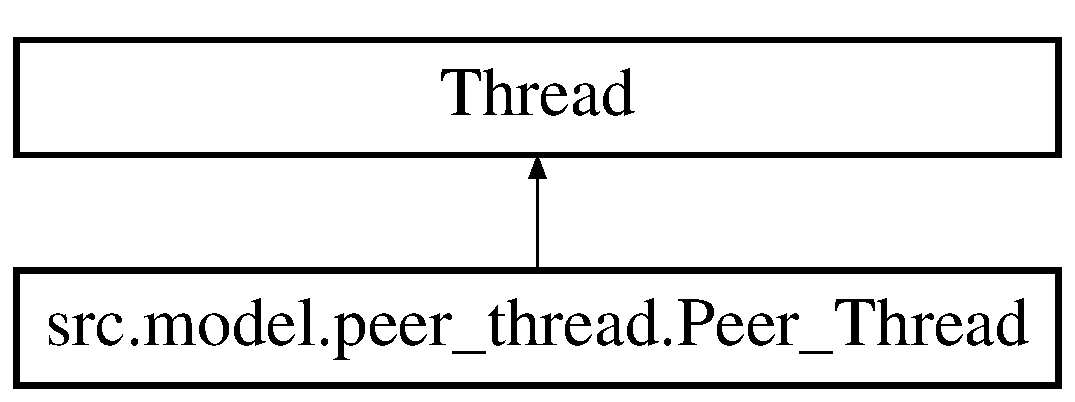
\includegraphics[height=2.000000cm]{classsrc_1_1model_1_1peer__thread_1_1Peer__Thread}
\end{center}
\end{figure}
\subsection*{Public Member Functions}
\begin{DoxyCompactItemize}
\item 
def \hyperlink{classsrc_1_1model_1_1peer__thread_1_1Peer__Thread_a218f79c8da03dc89d6bb437045a4e318}{\+\_\+\+\_\+init\+\_\+\+\_\+} (self, \hyperlink{classsrc_1_1model_1_1peer__thread_1_1Peer__Thread_a685ed6939daee9361c160842d392e21b}{thread\+I\+D}, \hyperlink{classsrc_1_1model_1_1peer__thread_1_1Peer__Thread_a44cb4ef7ef2b5647380fb76f4787b921}{name})
\item 
def \hyperlink{classsrc_1_1model_1_1peer__thread_1_1Peer__Thread_a62d6371381d0470f5b1b6965d29cfa29}{run} (self)
\end{DoxyCompactItemize}
\subsection*{Public Attributes}
\begin{DoxyCompactItemize}
\item 
\hyperlink{classsrc_1_1model_1_1peer__thread_1_1Peer__Thread_a245134f8422140117f14de3b5b9042ee}{peer\+\_\+active}
\item 
\hyperlink{classsrc_1_1model_1_1peer__thread_1_1Peer__Thread_a685ed6939daee9361c160842d392e21b}{thread\+I\+D}
\item 
\hyperlink{classsrc_1_1model_1_1peer__thread_1_1Peer__Thread_a44cb4ef7ef2b5647380fb76f4787b921}{name}
\item 
\hyperlink{classsrc_1_1model_1_1peer__thread_1_1Peer__Thread_a6f4887d821a57e79c96063f215b096ea}{x}
\end{DoxyCompactItemize}


\subsection{Constructor \& Destructor Documentation}
\hypertarget{classsrc_1_1model_1_1peer__thread_1_1Peer__Thread_a218f79c8da03dc89d6bb437045a4e318}{}\index{src\+::model\+::peer\+\_\+thread\+::\+Peer\+\_\+\+Thread@{src\+::model\+::peer\+\_\+thread\+::\+Peer\+\_\+\+Thread}!\+\_\+\+\_\+init\+\_\+\+\_\+@{\+\_\+\+\_\+init\+\_\+\+\_\+}}
\index{\+\_\+\+\_\+init\+\_\+\+\_\+@{\+\_\+\+\_\+init\+\_\+\+\_\+}!src\+::model\+::peer\+\_\+thread\+::\+Peer\+\_\+\+Thread@{src\+::model\+::peer\+\_\+thread\+::\+Peer\+\_\+\+Thread}}
\subsubsection[{\+\_\+\+\_\+init\+\_\+\+\_\+}]{\setlength{\rightskip}{0pt plus 5cm}def src.\+model.\+peer\+\_\+thread.\+Peer\+\_\+\+Thread.\+\_\+\+\_\+init\+\_\+\+\_\+ (
\begin{DoxyParamCaption}
\item[{}]{self, }
\item[{}]{thread\+I\+D, }
\item[{}]{name}
\end{DoxyParamCaption}
)}\label{classsrc_1_1model_1_1peer__thread_1_1Peer__Thread_a218f79c8da03dc89d6bb437045a4e318}


\subsection{Member Function Documentation}
\hypertarget{classsrc_1_1model_1_1peer__thread_1_1Peer__Thread_a62d6371381d0470f5b1b6965d29cfa29}{}\index{src\+::model\+::peer\+\_\+thread\+::\+Peer\+\_\+\+Thread@{src\+::model\+::peer\+\_\+thread\+::\+Peer\+\_\+\+Thread}!run@{run}}
\index{run@{run}!src\+::model\+::peer\+\_\+thread\+::\+Peer\+\_\+\+Thread@{src\+::model\+::peer\+\_\+thread\+::\+Peer\+\_\+\+Thread}}
\subsubsection[{run}]{\setlength{\rightskip}{0pt plus 5cm}def src.\+model.\+peer\+\_\+thread.\+Peer\+\_\+\+Thread.\+run (
\begin{DoxyParamCaption}
\item[{}]{self}
\end{DoxyParamCaption}
)}\label{classsrc_1_1model_1_1peer__thread_1_1Peer__Thread_a62d6371381d0470f5b1b6965d29cfa29}


\subsection{Member Data Documentation}
\hypertarget{classsrc_1_1model_1_1peer__thread_1_1Peer__Thread_a44cb4ef7ef2b5647380fb76f4787b921}{}\index{src\+::model\+::peer\+\_\+thread\+::\+Peer\+\_\+\+Thread@{src\+::model\+::peer\+\_\+thread\+::\+Peer\+\_\+\+Thread}!name@{name}}
\index{name@{name}!src\+::model\+::peer\+\_\+thread\+::\+Peer\+\_\+\+Thread@{src\+::model\+::peer\+\_\+thread\+::\+Peer\+\_\+\+Thread}}
\subsubsection[{name}]{\setlength{\rightskip}{0pt plus 5cm}src.\+model.\+peer\+\_\+thread.\+Peer\+\_\+\+Thread.\+name}\label{classsrc_1_1model_1_1peer__thread_1_1Peer__Thread_a44cb4ef7ef2b5647380fb76f4787b921}
\hypertarget{classsrc_1_1model_1_1peer__thread_1_1Peer__Thread_a245134f8422140117f14de3b5b9042ee}{}\index{src\+::model\+::peer\+\_\+thread\+::\+Peer\+\_\+\+Thread@{src\+::model\+::peer\+\_\+thread\+::\+Peer\+\_\+\+Thread}!peer\+\_\+active@{peer\+\_\+active}}
\index{peer\+\_\+active@{peer\+\_\+active}!src\+::model\+::peer\+\_\+thread\+::\+Peer\+\_\+\+Thread@{src\+::model\+::peer\+\_\+thread\+::\+Peer\+\_\+\+Thread}}
\subsubsection[{peer\+\_\+active}]{\setlength{\rightskip}{0pt plus 5cm}src.\+model.\+peer\+\_\+thread.\+Peer\+\_\+\+Thread.\+peer\+\_\+active}\label{classsrc_1_1model_1_1peer__thread_1_1Peer__Thread_a245134f8422140117f14de3b5b9042ee}
\hypertarget{classsrc_1_1model_1_1peer__thread_1_1Peer__Thread_a685ed6939daee9361c160842d392e21b}{}\index{src\+::model\+::peer\+\_\+thread\+::\+Peer\+\_\+\+Thread@{src\+::model\+::peer\+\_\+thread\+::\+Peer\+\_\+\+Thread}!thread\+I\+D@{thread\+I\+D}}
\index{thread\+I\+D@{thread\+I\+D}!src\+::model\+::peer\+\_\+thread\+::\+Peer\+\_\+\+Thread@{src\+::model\+::peer\+\_\+thread\+::\+Peer\+\_\+\+Thread}}
\subsubsection[{thread\+I\+D}]{\setlength{\rightskip}{0pt plus 5cm}src.\+model.\+peer\+\_\+thread.\+Peer\+\_\+\+Thread.\+thread\+I\+D}\label{classsrc_1_1model_1_1peer__thread_1_1Peer__Thread_a685ed6939daee9361c160842d392e21b}
\hypertarget{classsrc_1_1model_1_1peer__thread_1_1Peer__Thread_a6f4887d821a57e79c96063f215b096ea}{}\index{src\+::model\+::peer\+\_\+thread\+::\+Peer\+\_\+\+Thread@{src\+::model\+::peer\+\_\+thread\+::\+Peer\+\_\+\+Thread}!x@{x}}
\index{x@{x}!src\+::model\+::peer\+\_\+thread\+::\+Peer\+\_\+\+Thread@{src\+::model\+::peer\+\_\+thread\+::\+Peer\+\_\+\+Thread}}
\subsubsection[{x}]{\setlength{\rightskip}{0pt plus 5cm}src.\+model.\+peer\+\_\+thread.\+Peer\+\_\+\+Thread.\+x}\label{classsrc_1_1model_1_1peer__thread_1_1Peer__Thread_a6f4887d821a57e79c96063f215b096ea}


The documentation for this class was generated from the following file\+:\begin{DoxyCompactItemize}
\item 
src/model/\hyperlink{peer__thread_8py}{peer\+\_\+thread.\+py}\end{DoxyCompactItemize}

\hypertarget{classsrc_1_1lib_1_1vlc_1_1PlaybackMode}{}\section{src.\+lib.\+vlc.\+Playback\+Mode Class Reference}
\label{classsrc_1_1lib_1_1vlc_1_1PlaybackMode}\index{src.\+lib.\+vlc.\+Playback\+Mode@{src.\+lib.\+vlc.\+Playback\+Mode}}
Inheritance diagram for src.\+lib.\+vlc.\+Playback\+Mode\+:\begin{figure}[H]
\begin{center}
\leavevmode
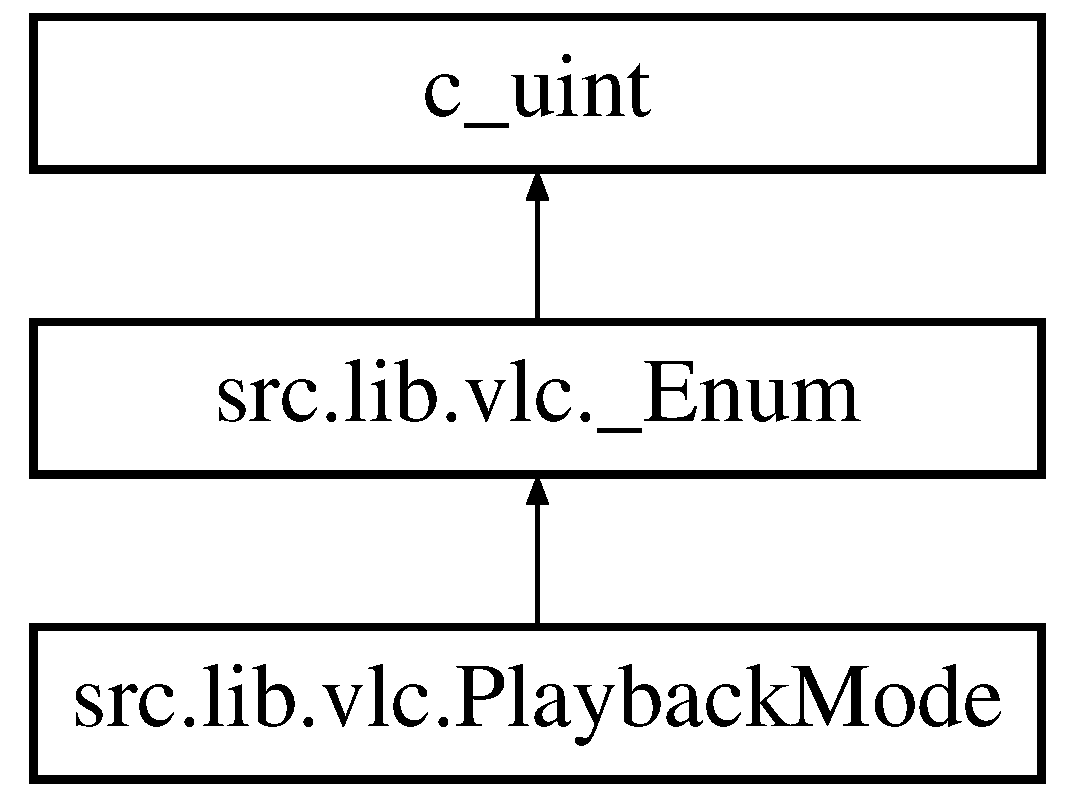
\includegraphics[height=3.000000cm]{classsrc_1_1lib_1_1vlc_1_1PlaybackMode}
\end{center}
\end{figure}
\subsection*{Static Private Attributes}
\begin{DoxyCompactItemize}
\item 
dictionary \hyperlink{classsrc_1_1lib_1_1vlc_1_1PlaybackMode_a0cd4cf4af9191357f19a9d0fb1246d06}{\+\_\+enum\+\_\+names\+\_\+}
\end{DoxyCompactItemize}
\subsection*{Additional Inherited Members}


\subsection{Detailed Description}
\begin{DoxyVerb}Defines playback modes for playlist.
\end{DoxyVerb}
 

\subsection{Member Data Documentation}
\hypertarget{classsrc_1_1lib_1_1vlc_1_1PlaybackMode_a0cd4cf4af9191357f19a9d0fb1246d06}{}\index{src\+::lib\+::vlc\+::\+Playback\+Mode@{src\+::lib\+::vlc\+::\+Playback\+Mode}!\+\_\+enum\+\_\+names\+\_\+@{\+\_\+enum\+\_\+names\+\_\+}}
\index{\+\_\+enum\+\_\+names\+\_\+@{\+\_\+enum\+\_\+names\+\_\+}!src\+::lib\+::vlc\+::\+Playback\+Mode@{src\+::lib\+::vlc\+::\+Playback\+Mode}}
\subsubsection[{\+\_\+enum\+\_\+names\+\_\+}]{\setlength{\rightskip}{0pt plus 5cm}dictionary src.\+lib.\+vlc.\+Playback\+Mode.\+\_\+enum\+\_\+names\+\_\+\hspace{0.3cm}{\ttfamily [static]}, {\ttfamily [private]}}\label{classsrc_1_1lib_1_1vlc_1_1PlaybackMode_a0cd4cf4af9191357f19a9d0fb1246d06}
{\bfseries Initial value\+:}
\begin{DoxyCode}
1 = \{
2         0: \textcolor{stringliteral}{'default'},
3         1: \textcolor{stringliteral}{'loop'},
4         2: \textcolor{stringliteral}{'repeat'},
5     \}
\end{DoxyCode}


The documentation for this class was generated from the following file\+:\begin{DoxyCompactItemize}
\item 
src/lib/\hyperlink{vlc_8py}{vlc.\+py}\end{DoxyCompactItemize}

\hypertarget{classsrc_1_1lib_1_1vlc_1_1PlaylistItem}{}\section{src.\+lib.\+vlc.\+Playlist\+Item Class Reference}
\label{classsrc_1_1lib_1_1vlc_1_1PlaylistItem}\index{src.\+lib.\+vlc.\+Playlist\+Item@{src.\+lib.\+vlc.\+Playlist\+Item}}
Inheritance diagram for src.\+lib.\+vlc.\+Playlist\+Item\+:\begin{figure}[H]
\begin{center}
\leavevmode
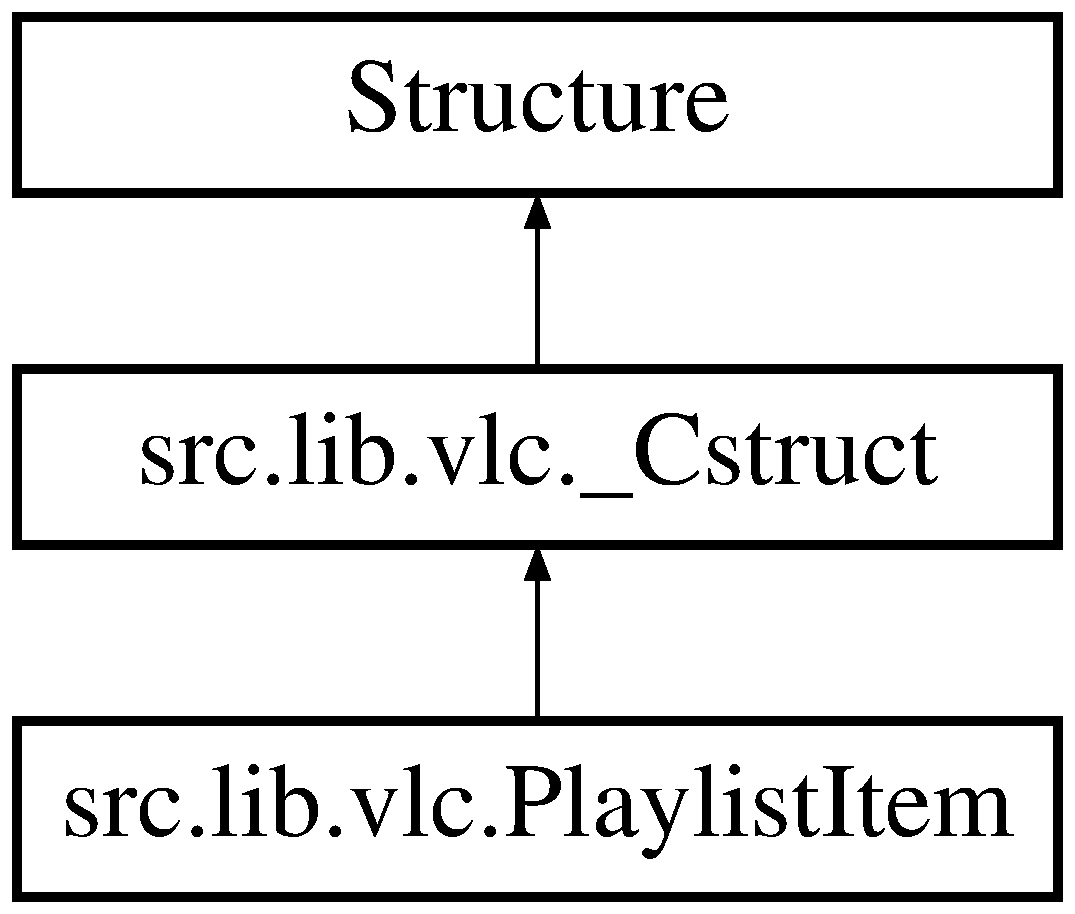
\includegraphics[height=3.000000cm]{classsrc_1_1lib_1_1vlc_1_1PlaylistItem}
\end{center}
\end{figure}
\subsection*{Public Member Functions}
\begin{DoxyCompactItemize}
\item 
def \hyperlink{classsrc_1_1lib_1_1vlc_1_1PlaylistItem_aae149d64fbf9e63a80d3d933b5b96c13}{\+\_\+\+\_\+str\+\_\+\+\_\+} (self)
\end{DoxyCompactItemize}
\subsection*{Static Private Attributes}
\begin{DoxyCompactItemize}
\item 
list \hyperlink{classsrc_1_1lib_1_1vlc_1_1PlaylistItem_a2c57ccd1c1c910833819ecf7af7aeb84}{\+\_\+fields\+\_\+}
\end{DoxyCompactItemize}


\subsection{Member Function Documentation}
\hypertarget{classsrc_1_1lib_1_1vlc_1_1PlaylistItem_aae149d64fbf9e63a80d3d933b5b96c13}{}\index{src\+::lib\+::vlc\+::\+Playlist\+Item@{src\+::lib\+::vlc\+::\+Playlist\+Item}!\+\_\+\+\_\+str\+\_\+\+\_\+@{\+\_\+\+\_\+str\+\_\+\+\_\+}}
\index{\+\_\+\+\_\+str\+\_\+\+\_\+@{\+\_\+\+\_\+str\+\_\+\+\_\+}!src\+::lib\+::vlc\+::\+Playlist\+Item@{src\+::lib\+::vlc\+::\+Playlist\+Item}}
\subsubsection[{\+\_\+\+\_\+str\+\_\+\+\_\+}]{\setlength{\rightskip}{0pt plus 5cm}def src.\+lib.\+vlc.\+Playlist\+Item.\+\_\+\+\_\+str\+\_\+\+\_\+ (
\begin{DoxyParamCaption}
\item[{}]{self}
\end{DoxyParamCaption}
)}\label{classsrc_1_1lib_1_1vlc_1_1PlaylistItem_aae149d64fbf9e63a80d3d933b5b96c13}


\subsection{Member Data Documentation}
\hypertarget{classsrc_1_1lib_1_1vlc_1_1PlaylistItem_a2c57ccd1c1c910833819ecf7af7aeb84}{}\index{src\+::lib\+::vlc\+::\+Playlist\+Item@{src\+::lib\+::vlc\+::\+Playlist\+Item}!\+\_\+fields\+\_\+@{\+\_\+fields\+\_\+}}
\index{\+\_\+fields\+\_\+@{\+\_\+fields\+\_\+}!src\+::lib\+::vlc\+::\+Playlist\+Item@{src\+::lib\+::vlc\+::\+Playlist\+Item}}
\subsubsection[{\+\_\+fields\+\_\+}]{\setlength{\rightskip}{0pt plus 5cm}list src.\+lib.\+vlc.\+Playlist\+Item.\+\_\+fields\+\_\+\hspace{0.3cm}{\ttfamily [static]}, {\ttfamily [private]}}\label{classsrc_1_1lib_1_1vlc_1_1PlaylistItem_a2c57ccd1c1c910833819ecf7af7aeb84}
{\bfseries Initial value\+:}
\begin{DoxyCode}
1 = [
2         (\textcolor{stringliteral}{'id'},   ctypes.c\_int   ),
3         (\textcolor{stringliteral}{'uri'},  ctypes.c\_char\_p),
4         (\textcolor{stringliteral}{'name'}, ctypes.c\_char\_p),
5     ]
\end{DoxyCode}


The documentation for this class was generated from the following file\+:\begin{DoxyCompactItemize}
\item 
src/lib/\hyperlink{vlc_8py}{vlc.\+py}\end{DoxyCompactItemize}

\hypertarget{classsrc_1_1lib_1_1vlc_1_1Position}{}\section{src.\+lib.\+vlc.\+Position Class Reference}
\label{classsrc_1_1lib_1_1vlc_1_1Position}\index{src.\+lib.\+vlc.\+Position@{src.\+lib.\+vlc.\+Position}}
Inheritance diagram for src.\+lib.\+vlc.\+Position\+:\begin{figure}[H]
\begin{center}
\leavevmode
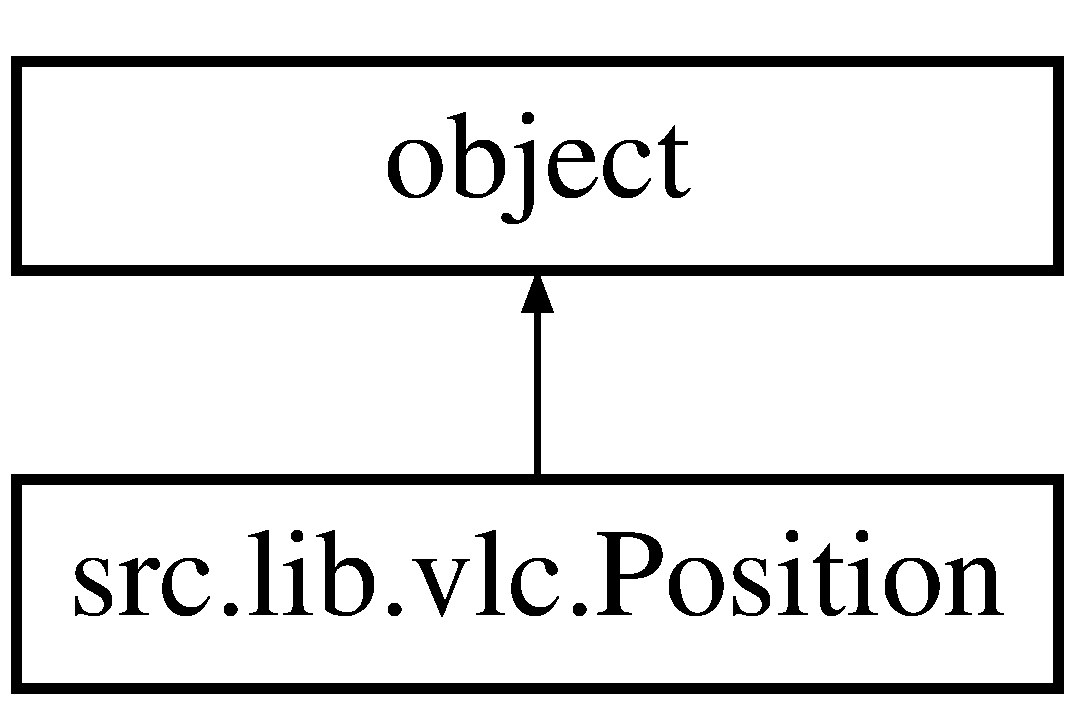
\includegraphics[height=2.000000cm]{classsrc_1_1lib_1_1vlc_1_1Position}
\end{center}
\end{figure}
\subsection*{Public Member Functions}
\begin{DoxyCompactItemize}
\item 
def \hyperlink{classsrc_1_1lib_1_1vlc_1_1Position_aff6d8088b0c575264cda6ce64d2d4a0d}{\+\_\+\+\_\+init\+\_\+\+\_\+} (self, unused)
\item 
def \hyperlink{classsrc_1_1lib_1_1vlc_1_1Position_ade091a758dbe1bb2acbf9e9ae7c395a9}{\+\_\+\+\_\+setattr\+\_\+\+\_\+} (self, unused)
\end{DoxyCompactItemize}
\subsection*{Static Public Attributes}
\begin{DoxyCompactItemize}
\item 
int \hyperlink{classsrc_1_1lib_1_1vlc_1_1Position_a6b5a5b27d026829e0fbde98e8939e35c}{Center} = 0
\item 
int \hyperlink{classsrc_1_1lib_1_1vlc_1_1Position_a1ad4c8b4826b8c6c4ca45f15d12c2d4e}{Left} = 1
\item 
int \hyperlink{classsrc_1_1lib_1_1vlc_1_1Position_a8e8cb34b617c818abc7a265de5a7bddd}{Center\+Left} = 1
\item 
int \hyperlink{classsrc_1_1lib_1_1vlc_1_1Position_a2c76f0a94b3f2da73519ca4a5aeecacf}{Right} = 2
\item 
int \hyperlink{classsrc_1_1lib_1_1vlc_1_1Position_a9664a8d6ba8949d4e97573d6d10c7cd0}{Center\+Right} = 2
\item 
int \hyperlink{classsrc_1_1lib_1_1vlc_1_1Position_a46af24dbbd6ccf39f59faf345d5e3665}{Top} = 4
\item 
int \hyperlink{classsrc_1_1lib_1_1vlc_1_1Position_aa392a087c67e88221021ac3d02ffc5f3}{Top\+Center} = 4
\item 
int \hyperlink{classsrc_1_1lib_1_1vlc_1_1Position_aa9558cfe443d5abddd3151e45c3d76e4}{Top\+Left} = 5
\item 
int \hyperlink{classsrc_1_1lib_1_1vlc_1_1Position_af9105f2d6bed5aee191e95074620f987}{Top\+Right} = 6
\item 
int \hyperlink{classsrc_1_1lib_1_1vlc_1_1Position_ae5b5cbe73de6f40f62242f293b1a9a37}{Bottom} = 8
\item 
int \hyperlink{classsrc_1_1lib_1_1vlc_1_1Position_a1ffdc1354b96080984fc0c57bc0c02a8}{Bottom\+Center} = 8
\item 
int \hyperlink{classsrc_1_1lib_1_1vlc_1_1Position_aa610f54296adc368c1f82174e962656f}{Bottom\+Left} = 9
\item 
int \hyperlink{classsrc_1_1lib_1_1vlc_1_1Position_ad1ec1f4676a03b72161301f3df36738e}{Bottom\+Right} = 10
\end{DoxyCompactItemize}


\subsection{Detailed Description}
\begin{DoxyVerb}Enum-like, immutable window position constants.

   See e.g. VideoMarqueeOption.Position.
\end{DoxyVerb}
 

\subsection{Constructor \& Destructor Documentation}
\hypertarget{classsrc_1_1lib_1_1vlc_1_1Position_aff6d8088b0c575264cda6ce64d2d4a0d}{}\index{src\+::lib\+::vlc\+::\+Position@{src\+::lib\+::vlc\+::\+Position}!\+\_\+\+\_\+init\+\_\+\+\_\+@{\+\_\+\+\_\+init\+\_\+\+\_\+}}
\index{\+\_\+\+\_\+init\+\_\+\+\_\+@{\+\_\+\+\_\+init\+\_\+\+\_\+}!src\+::lib\+::vlc\+::\+Position@{src\+::lib\+::vlc\+::\+Position}}
\subsubsection[{\+\_\+\+\_\+init\+\_\+\+\_\+}]{\setlength{\rightskip}{0pt plus 5cm}def src.\+lib.\+vlc.\+Position.\+\_\+\+\_\+init\+\_\+\+\_\+ (
\begin{DoxyParamCaption}
\item[{}]{self, }
\item[{}]{unused}
\end{DoxyParamCaption}
)}\label{classsrc_1_1lib_1_1vlc_1_1Position_aff6d8088b0c575264cda6ce64d2d4a0d}


\subsection{Member Function Documentation}
\hypertarget{classsrc_1_1lib_1_1vlc_1_1Position_ade091a758dbe1bb2acbf9e9ae7c395a9}{}\index{src\+::lib\+::vlc\+::\+Position@{src\+::lib\+::vlc\+::\+Position}!\+\_\+\+\_\+setattr\+\_\+\+\_\+@{\+\_\+\+\_\+setattr\+\_\+\+\_\+}}
\index{\+\_\+\+\_\+setattr\+\_\+\+\_\+@{\+\_\+\+\_\+setattr\+\_\+\+\_\+}!src\+::lib\+::vlc\+::\+Position@{src\+::lib\+::vlc\+::\+Position}}
\subsubsection[{\+\_\+\+\_\+setattr\+\_\+\+\_\+}]{\setlength{\rightskip}{0pt plus 5cm}def src.\+lib.\+vlc.\+Position.\+\_\+\+\_\+setattr\+\_\+\+\_\+ (
\begin{DoxyParamCaption}
\item[{}]{self, }
\item[{}]{unused}
\end{DoxyParamCaption}
)}\label{classsrc_1_1lib_1_1vlc_1_1Position_ade091a758dbe1bb2acbf9e9ae7c395a9}


\subsection{Member Data Documentation}
\hypertarget{classsrc_1_1lib_1_1vlc_1_1Position_ae5b5cbe73de6f40f62242f293b1a9a37}{}\index{src\+::lib\+::vlc\+::\+Position@{src\+::lib\+::vlc\+::\+Position}!Bottom@{Bottom}}
\index{Bottom@{Bottom}!src\+::lib\+::vlc\+::\+Position@{src\+::lib\+::vlc\+::\+Position}}
\subsubsection[{Bottom}]{\setlength{\rightskip}{0pt plus 5cm}int src.\+lib.\+vlc.\+Position.\+Bottom = 8\hspace{0.3cm}{\ttfamily [static]}}\label{classsrc_1_1lib_1_1vlc_1_1Position_ae5b5cbe73de6f40f62242f293b1a9a37}
\hypertarget{classsrc_1_1lib_1_1vlc_1_1Position_a1ffdc1354b96080984fc0c57bc0c02a8}{}\index{src\+::lib\+::vlc\+::\+Position@{src\+::lib\+::vlc\+::\+Position}!Bottom\+Center@{Bottom\+Center}}
\index{Bottom\+Center@{Bottom\+Center}!src\+::lib\+::vlc\+::\+Position@{src\+::lib\+::vlc\+::\+Position}}
\subsubsection[{Bottom\+Center}]{\setlength{\rightskip}{0pt plus 5cm}int src.\+lib.\+vlc.\+Position.\+Bottom\+Center = 8\hspace{0.3cm}{\ttfamily [static]}}\label{classsrc_1_1lib_1_1vlc_1_1Position_a1ffdc1354b96080984fc0c57bc0c02a8}
\hypertarget{classsrc_1_1lib_1_1vlc_1_1Position_aa610f54296adc368c1f82174e962656f}{}\index{src\+::lib\+::vlc\+::\+Position@{src\+::lib\+::vlc\+::\+Position}!Bottom\+Left@{Bottom\+Left}}
\index{Bottom\+Left@{Bottom\+Left}!src\+::lib\+::vlc\+::\+Position@{src\+::lib\+::vlc\+::\+Position}}
\subsubsection[{Bottom\+Left}]{\setlength{\rightskip}{0pt plus 5cm}int src.\+lib.\+vlc.\+Position.\+Bottom\+Left = 9\hspace{0.3cm}{\ttfamily [static]}}\label{classsrc_1_1lib_1_1vlc_1_1Position_aa610f54296adc368c1f82174e962656f}
\hypertarget{classsrc_1_1lib_1_1vlc_1_1Position_ad1ec1f4676a03b72161301f3df36738e}{}\index{src\+::lib\+::vlc\+::\+Position@{src\+::lib\+::vlc\+::\+Position}!Bottom\+Right@{Bottom\+Right}}
\index{Bottom\+Right@{Bottom\+Right}!src\+::lib\+::vlc\+::\+Position@{src\+::lib\+::vlc\+::\+Position}}
\subsubsection[{Bottom\+Right}]{\setlength{\rightskip}{0pt plus 5cm}int src.\+lib.\+vlc.\+Position.\+Bottom\+Right = 10\hspace{0.3cm}{\ttfamily [static]}}\label{classsrc_1_1lib_1_1vlc_1_1Position_ad1ec1f4676a03b72161301f3df36738e}
\hypertarget{classsrc_1_1lib_1_1vlc_1_1Position_a6b5a5b27d026829e0fbde98e8939e35c}{}\index{src\+::lib\+::vlc\+::\+Position@{src\+::lib\+::vlc\+::\+Position}!Center@{Center}}
\index{Center@{Center}!src\+::lib\+::vlc\+::\+Position@{src\+::lib\+::vlc\+::\+Position}}
\subsubsection[{Center}]{\setlength{\rightskip}{0pt plus 5cm}int src.\+lib.\+vlc.\+Position.\+Center = 0\hspace{0.3cm}{\ttfamily [static]}}\label{classsrc_1_1lib_1_1vlc_1_1Position_a6b5a5b27d026829e0fbde98e8939e35c}
\hypertarget{classsrc_1_1lib_1_1vlc_1_1Position_a8e8cb34b617c818abc7a265de5a7bddd}{}\index{src\+::lib\+::vlc\+::\+Position@{src\+::lib\+::vlc\+::\+Position}!Center\+Left@{Center\+Left}}
\index{Center\+Left@{Center\+Left}!src\+::lib\+::vlc\+::\+Position@{src\+::lib\+::vlc\+::\+Position}}
\subsubsection[{Center\+Left}]{\setlength{\rightskip}{0pt plus 5cm}int src.\+lib.\+vlc.\+Position.\+Center\+Left = 1\hspace{0.3cm}{\ttfamily [static]}}\label{classsrc_1_1lib_1_1vlc_1_1Position_a8e8cb34b617c818abc7a265de5a7bddd}
\hypertarget{classsrc_1_1lib_1_1vlc_1_1Position_a9664a8d6ba8949d4e97573d6d10c7cd0}{}\index{src\+::lib\+::vlc\+::\+Position@{src\+::lib\+::vlc\+::\+Position}!Center\+Right@{Center\+Right}}
\index{Center\+Right@{Center\+Right}!src\+::lib\+::vlc\+::\+Position@{src\+::lib\+::vlc\+::\+Position}}
\subsubsection[{Center\+Right}]{\setlength{\rightskip}{0pt plus 5cm}int src.\+lib.\+vlc.\+Position.\+Center\+Right = 2\hspace{0.3cm}{\ttfamily [static]}}\label{classsrc_1_1lib_1_1vlc_1_1Position_a9664a8d6ba8949d4e97573d6d10c7cd0}
\hypertarget{classsrc_1_1lib_1_1vlc_1_1Position_a1ad4c8b4826b8c6c4ca45f15d12c2d4e}{}\index{src\+::lib\+::vlc\+::\+Position@{src\+::lib\+::vlc\+::\+Position}!Left@{Left}}
\index{Left@{Left}!src\+::lib\+::vlc\+::\+Position@{src\+::lib\+::vlc\+::\+Position}}
\subsubsection[{Left}]{\setlength{\rightskip}{0pt plus 5cm}int src.\+lib.\+vlc.\+Position.\+Left = 1\hspace{0.3cm}{\ttfamily [static]}}\label{classsrc_1_1lib_1_1vlc_1_1Position_a1ad4c8b4826b8c6c4ca45f15d12c2d4e}
\hypertarget{classsrc_1_1lib_1_1vlc_1_1Position_a2c76f0a94b3f2da73519ca4a5aeecacf}{}\index{src\+::lib\+::vlc\+::\+Position@{src\+::lib\+::vlc\+::\+Position}!Right@{Right}}
\index{Right@{Right}!src\+::lib\+::vlc\+::\+Position@{src\+::lib\+::vlc\+::\+Position}}
\subsubsection[{Right}]{\setlength{\rightskip}{0pt plus 5cm}int src.\+lib.\+vlc.\+Position.\+Right = 2\hspace{0.3cm}{\ttfamily [static]}}\label{classsrc_1_1lib_1_1vlc_1_1Position_a2c76f0a94b3f2da73519ca4a5aeecacf}
\hypertarget{classsrc_1_1lib_1_1vlc_1_1Position_a46af24dbbd6ccf39f59faf345d5e3665}{}\index{src\+::lib\+::vlc\+::\+Position@{src\+::lib\+::vlc\+::\+Position}!Top@{Top}}
\index{Top@{Top}!src\+::lib\+::vlc\+::\+Position@{src\+::lib\+::vlc\+::\+Position}}
\subsubsection[{Top}]{\setlength{\rightskip}{0pt plus 5cm}int src.\+lib.\+vlc.\+Position.\+Top = 4\hspace{0.3cm}{\ttfamily [static]}}\label{classsrc_1_1lib_1_1vlc_1_1Position_a46af24dbbd6ccf39f59faf345d5e3665}
\hypertarget{classsrc_1_1lib_1_1vlc_1_1Position_aa392a087c67e88221021ac3d02ffc5f3}{}\index{src\+::lib\+::vlc\+::\+Position@{src\+::lib\+::vlc\+::\+Position}!Top\+Center@{Top\+Center}}
\index{Top\+Center@{Top\+Center}!src\+::lib\+::vlc\+::\+Position@{src\+::lib\+::vlc\+::\+Position}}
\subsubsection[{Top\+Center}]{\setlength{\rightskip}{0pt plus 5cm}int src.\+lib.\+vlc.\+Position.\+Top\+Center = 4\hspace{0.3cm}{\ttfamily [static]}}\label{classsrc_1_1lib_1_1vlc_1_1Position_aa392a087c67e88221021ac3d02ffc5f3}
\hypertarget{classsrc_1_1lib_1_1vlc_1_1Position_aa9558cfe443d5abddd3151e45c3d76e4}{}\index{src\+::lib\+::vlc\+::\+Position@{src\+::lib\+::vlc\+::\+Position}!Top\+Left@{Top\+Left}}
\index{Top\+Left@{Top\+Left}!src\+::lib\+::vlc\+::\+Position@{src\+::lib\+::vlc\+::\+Position}}
\subsubsection[{Top\+Left}]{\setlength{\rightskip}{0pt plus 5cm}int src.\+lib.\+vlc.\+Position.\+Top\+Left = 5\hspace{0.3cm}{\ttfamily [static]}}\label{classsrc_1_1lib_1_1vlc_1_1Position_aa9558cfe443d5abddd3151e45c3d76e4}
\hypertarget{classsrc_1_1lib_1_1vlc_1_1Position_af9105f2d6bed5aee191e95074620f987}{}\index{src\+::lib\+::vlc\+::\+Position@{src\+::lib\+::vlc\+::\+Position}!Top\+Right@{Top\+Right}}
\index{Top\+Right@{Top\+Right}!src\+::lib\+::vlc\+::\+Position@{src\+::lib\+::vlc\+::\+Position}}
\subsubsection[{Top\+Right}]{\setlength{\rightskip}{0pt plus 5cm}int src.\+lib.\+vlc.\+Position.\+Top\+Right = 6\hspace{0.3cm}{\ttfamily [static]}}\label{classsrc_1_1lib_1_1vlc_1_1Position_af9105f2d6bed5aee191e95074620f987}


The documentation for this class was generated from the following file\+:\begin{DoxyCompactItemize}
\item 
src/lib/\hyperlink{vlc_8py}{vlc.\+py}\end{DoxyCompactItemize}

\hypertarget{classsrc_1_1lib_1_1vlc_1_1Rectangle}{}\section{src.\+lib.\+vlc.\+Rectangle Class Reference}
\label{classsrc_1_1lib_1_1vlc_1_1Rectangle}\index{src.\+lib.\+vlc.\+Rectangle@{src.\+lib.\+vlc.\+Rectangle}}
Inheritance diagram for src.\+lib.\+vlc.\+Rectangle\+:\begin{figure}[H]
\begin{center}
\leavevmode
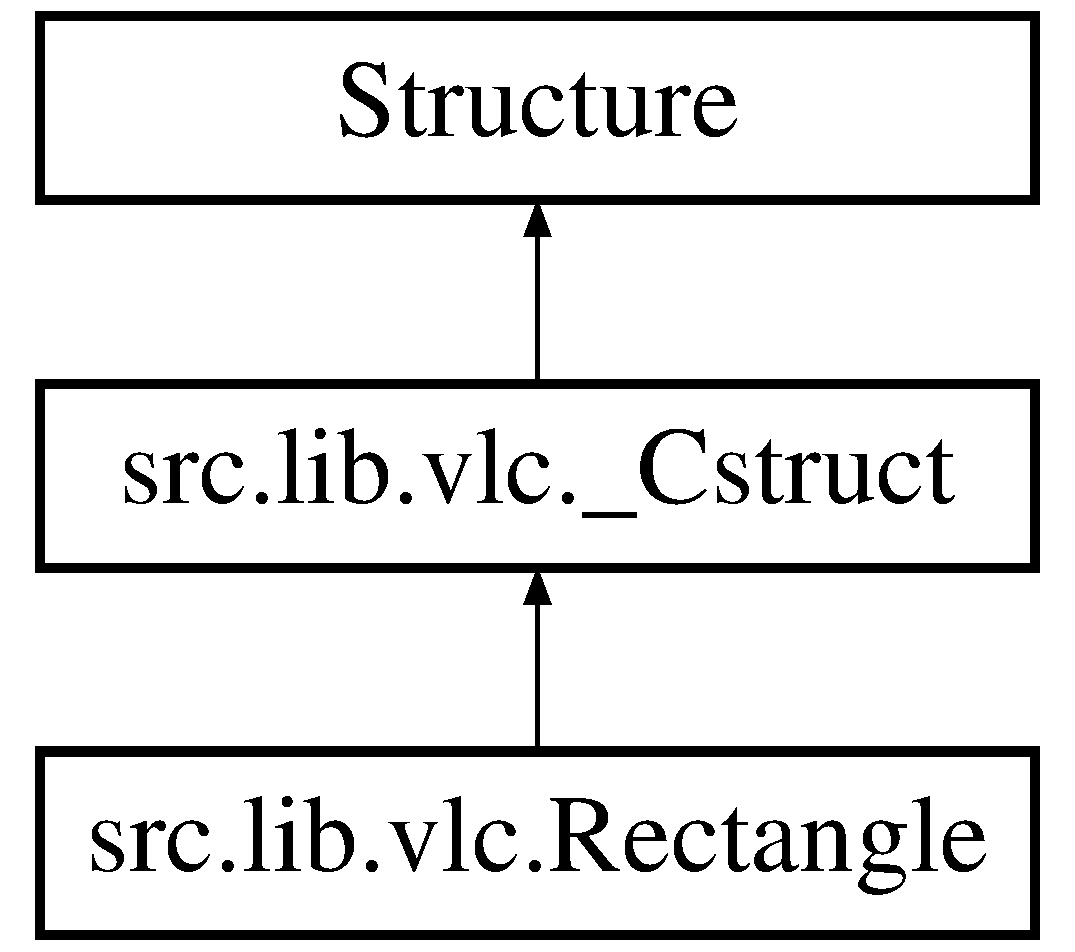
\includegraphics[height=3.000000cm]{classsrc_1_1lib_1_1vlc_1_1Rectangle}
\end{center}
\end{figure}
\subsection*{Static Private Attributes}
\begin{DoxyCompactItemize}
\item 
list \hyperlink{classsrc_1_1lib_1_1vlc_1_1Rectangle_afaeec066d99b840e72a6bff71e02536c}{\+\_\+fields\+\_\+}
\end{DoxyCompactItemize}
\subsection*{Additional Inherited Members}


\subsection{Member Data Documentation}
\hypertarget{classsrc_1_1lib_1_1vlc_1_1Rectangle_afaeec066d99b840e72a6bff71e02536c}{}\index{src\+::lib\+::vlc\+::\+Rectangle@{src\+::lib\+::vlc\+::\+Rectangle}!\+\_\+fields\+\_\+@{\+\_\+fields\+\_\+}}
\index{\+\_\+fields\+\_\+@{\+\_\+fields\+\_\+}!src\+::lib\+::vlc\+::\+Rectangle@{src\+::lib\+::vlc\+::\+Rectangle}}
\subsubsection[{\+\_\+fields\+\_\+}]{\setlength{\rightskip}{0pt plus 5cm}list src.\+lib.\+vlc.\+Rectangle.\+\_\+fields\+\_\+\hspace{0.3cm}{\ttfamily [static]}, {\ttfamily [private]}}\label{classsrc_1_1lib_1_1vlc_1_1Rectangle_afaeec066d99b840e72a6bff71e02536c}
{\bfseries Initial value\+:}
\begin{DoxyCode}
1 = [
2         (\textcolor{stringliteral}{'top'},    ctypes.c\_int),
3         (\textcolor{stringliteral}{'left'},   ctypes.c\_int),
4         (\textcolor{stringliteral}{'bottom'}, ctypes.c\_int),
5         (\textcolor{stringliteral}{'right'},  ctypes.c\_int),
6     ]
\end{DoxyCode}


The documentation for this class was generated from the following file\+:\begin{DoxyCompactItemize}
\item 
src/lib/\hyperlink{vlc_8py}{vlc.\+py}\end{DoxyCompactItemize}

\hypertarget{classsrc_1_1adapter_1_1speed__adapter_1_1Speed__Adapter}{}\section{src.\+adapter.\+speed\+\_\+adapter.\+Speed\+\_\+\+Adapter Class Reference}
\label{classsrc_1_1adapter_1_1speed__adapter_1_1Speed__Adapter}\index{src.\+adapter.\+speed\+\_\+adapter.\+Speed\+\_\+\+Adapter@{src.\+adapter.\+speed\+\_\+adapter.\+Speed\+\_\+\+Adapter}}
\subsection*{Public Member Functions}
\begin{DoxyCompactItemize}
\item 
def \hyperlink{classsrc_1_1adapter_1_1speed__adapter_1_1Speed__Adapter_a3d8fac7caed6745662def3d800c44c6f}{set\+\_\+widget} (self, down\+\_\+label, up\+\_\+label, users\+\_\+label)
\end{DoxyCompactItemize}
\subsection*{Static Public Attributes}
\begin{DoxyCompactItemize}
\item 
\hyperlink{classsrc_1_1adapter_1_1speed__adapter_1_1Speed__Adapter_a8c3f1760b329c8da444488fd50f1a128}{U\+P\+\_\+\+W\+I\+D\+G\+E\+T} = None
\item 
\hyperlink{classsrc_1_1adapter_1_1speed__adapter_1_1Speed__Adapter_ae7ae8ac17406badcb53a0b2b90127f41}{D\+O\+W\+N\+\_\+\+W\+I\+D\+G\+E\+T} = None
\item 
\hyperlink{classsrc_1_1adapter_1_1speed__adapter_1_1Speed__Adapter_a02e9c7a2cd8b9d8c8a9dc8921ba32768}{U\+S\+E\+R\+S\+\_\+\+W\+I\+D\+G\+E\+T} = None
\end{DoxyCompactItemize}


\subsection{Member Function Documentation}
\hypertarget{classsrc_1_1adapter_1_1speed__adapter_1_1Speed__Adapter_a3d8fac7caed6745662def3d800c44c6f}{}\index{src\+::adapter\+::speed\+\_\+adapter\+::\+Speed\+\_\+\+Adapter@{src\+::adapter\+::speed\+\_\+adapter\+::\+Speed\+\_\+\+Adapter}!set\+\_\+widget@{set\+\_\+widget}}
\index{set\+\_\+widget@{set\+\_\+widget}!src\+::adapter\+::speed\+\_\+adapter\+::\+Speed\+\_\+\+Adapter@{src\+::adapter\+::speed\+\_\+adapter\+::\+Speed\+\_\+\+Adapter}}
\subsubsection[{set\+\_\+widget}]{\setlength{\rightskip}{0pt plus 5cm}def src.\+adapter.\+speed\+\_\+adapter.\+Speed\+\_\+\+Adapter.\+set\+\_\+widget (
\begin{DoxyParamCaption}
\item[{}]{self, }
\item[{}]{down\+\_\+label, }
\item[{}]{up\+\_\+label, }
\item[{}]{users\+\_\+label}
\end{DoxyParamCaption}
)}\label{classsrc_1_1adapter_1_1speed__adapter_1_1Speed__Adapter_a3d8fac7caed6745662def3d800c44c6f}


\subsection{Member Data Documentation}
\hypertarget{classsrc_1_1adapter_1_1speed__adapter_1_1Speed__Adapter_ae7ae8ac17406badcb53a0b2b90127f41}{}\index{src\+::adapter\+::speed\+\_\+adapter\+::\+Speed\+\_\+\+Adapter@{src\+::adapter\+::speed\+\_\+adapter\+::\+Speed\+\_\+\+Adapter}!D\+O\+W\+N\+\_\+\+W\+I\+D\+G\+E\+T@{D\+O\+W\+N\+\_\+\+W\+I\+D\+G\+E\+T}}
\index{D\+O\+W\+N\+\_\+\+W\+I\+D\+G\+E\+T@{D\+O\+W\+N\+\_\+\+W\+I\+D\+G\+E\+T}!src\+::adapter\+::speed\+\_\+adapter\+::\+Speed\+\_\+\+Adapter@{src\+::adapter\+::speed\+\_\+adapter\+::\+Speed\+\_\+\+Adapter}}
\subsubsection[{D\+O\+W\+N\+\_\+\+W\+I\+D\+G\+E\+T}]{\setlength{\rightskip}{0pt plus 5cm}src.\+adapter.\+speed\+\_\+adapter.\+Speed\+\_\+\+Adapter.\+D\+O\+W\+N\+\_\+\+W\+I\+D\+G\+E\+T = None\hspace{0.3cm}{\ttfamily [static]}}\label{classsrc_1_1adapter_1_1speed__adapter_1_1Speed__Adapter_ae7ae8ac17406badcb53a0b2b90127f41}
\hypertarget{classsrc_1_1adapter_1_1speed__adapter_1_1Speed__Adapter_a8c3f1760b329c8da444488fd50f1a128}{}\index{src\+::adapter\+::speed\+\_\+adapter\+::\+Speed\+\_\+\+Adapter@{src\+::adapter\+::speed\+\_\+adapter\+::\+Speed\+\_\+\+Adapter}!U\+P\+\_\+\+W\+I\+D\+G\+E\+T@{U\+P\+\_\+\+W\+I\+D\+G\+E\+T}}
\index{U\+P\+\_\+\+W\+I\+D\+G\+E\+T@{U\+P\+\_\+\+W\+I\+D\+G\+E\+T}!src\+::adapter\+::speed\+\_\+adapter\+::\+Speed\+\_\+\+Adapter@{src\+::adapter\+::speed\+\_\+adapter\+::\+Speed\+\_\+\+Adapter}}
\subsubsection[{U\+P\+\_\+\+W\+I\+D\+G\+E\+T}]{\setlength{\rightskip}{0pt plus 5cm}src.\+adapter.\+speed\+\_\+adapter.\+Speed\+\_\+\+Adapter.\+U\+P\+\_\+\+W\+I\+D\+G\+E\+T = None\hspace{0.3cm}{\ttfamily [static]}}\label{classsrc_1_1adapter_1_1speed__adapter_1_1Speed__Adapter_a8c3f1760b329c8da444488fd50f1a128}
\hypertarget{classsrc_1_1adapter_1_1speed__adapter_1_1Speed__Adapter_a02e9c7a2cd8b9d8c8a9dc8921ba32768}{}\index{src\+::adapter\+::speed\+\_\+adapter\+::\+Speed\+\_\+\+Adapter@{src\+::adapter\+::speed\+\_\+adapter\+::\+Speed\+\_\+\+Adapter}!U\+S\+E\+R\+S\+\_\+\+W\+I\+D\+G\+E\+T@{U\+S\+E\+R\+S\+\_\+\+W\+I\+D\+G\+E\+T}}
\index{U\+S\+E\+R\+S\+\_\+\+W\+I\+D\+G\+E\+T@{U\+S\+E\+R\+S\+\_\+\+W\+I\+D\+G\+E\+T}!src\+::adapter\+::speed\+\_\+adapter\+::\+Speed\+\_\+\+Adapter@{src\+::adapter\+::speed\+\_\+adapter\+::\+Speed\+\_\+\+Adapter}}
\subsubsection[{U\+S\+E\+R\+S\+\_\+\+W\+I\+D\+G\+E\+T}]{\setlength{\rightskip}{0pt plus 5cm}src.\+adapter.\+speed\+\_\+adapter.\+Speed\+\_\+\+Adapter.\+U\+S\+E\+R\+S\+\_\+\+W\+I\+D\+G\+E\+T = None\hspace{0.3cm}{\ttfamily [static]}}\label{classsrc_1_1adapter_1_1speed__adapter_1_1Speed__Adapter_a02e9c7a2cd8b9d8c8a9dc8921ba32768}


The documentation for this class was generated from the following file\+:\begin{DoxyCompactItemize}
\item 
src/adapter/\hyperlink{speed__adapter_8py}{speed\+\_\+adapter.\+py}\end{DoxyCompactItemize}

\hypertarget{classsrc_1_1core_1_1splitter_1_1Splitter}{}\section{src.\+core.\+splitter.\+Splitter Class Reference}
\label{classsrc_1_1core_1_1splitter_1_1Splitter}\index{src.\+core.\+splitter.\+Splitter@{src.\+core.\+splitter.\+Splitter}}
\subsection*{Public Member Functions}
\begin{DoxyCompactItemize}
\item 
def \hyperlink{classsrc_1_1core_1_1splitter_1_1Splitter_a15c464b21aba83242931d05cb81bd0e9}{\+\_\+\+\_\+init\+\_\+\+\_\+} (self)
\end{DoxyCompactItemize}


\subsection{Constructor \& Destructor Documentation}
\hypertarget{classsrc_1_1core_1_1splitter_1_1Splitter_a15c464b21aba83242931d05cb81bd0e9}{}\index{src\+::core\+::splitter\+::\+Splitter@{src\+::core\+::splitter\+::\+Splitter}!\+\_\+\+\_\+init\+\_\+\+\_\+@{\+\_\+\+\_\+init\+\_\+\+\_\+}}
\index{\+\_\+\+\_\+init\+\_\+\+\_\+@{\+\_\+\+\_\+init\+\_\+\+\_\+}!src\+::core\+::splitter\+::\+Splitter@{src\+::core\+::splitter\+::\+Splitter}}
\subsubsection[{\+\_\+\+\_\+init\+\_\+\+\_\+}]{\setlength{\rightskip}{0pt plus 5cm}def src.\+core.\+splitter.\+Splitter.\+\_\+\+\_\+init\+\_\+\+\_\+ (
\begin{DoxyParamCaption}
\item[{}]{self}
\end{DoxyParamCaption}
)}\label{classsrc_1_1core_1_1splitter_1_1Splitter_a15c464b21aba83242931d05cb81bd0e9}


The documentation for this class was generated from the following file\+:\begin{DoxyCompactItemize}
\item 
src/core/\hyperlink{splitter_8py}{splitter.\+py}\end{DoxyCompactItemize}

\hypertarget{classsrc_1_1core_1_1splitter__acs_1_1Splitter__ACS}{}\section{src.\+core.\+splitter\+\_\+acs.\+Splitter\+\_\+\+A\+C\+S Class Reference}
\label{classsrc_1_1core_1_1splitter__acs_1_1Splitter__ACS}\index{src.\+core.\+splitter\+\_\+acs.\+Splitter\+\_\+\+A\+C\+S@{src.\+core.\+splitter\+\_\+acs.\+Splitter\+\_\+\+A\+C\+S}}
Inheritance diagram for src.\+core.\+splitter\+\_\+acs.\+Splitter\+\_\+\+A\+C\+S\+:\begin{figure}[H]
\begin{center}
\leavevmode
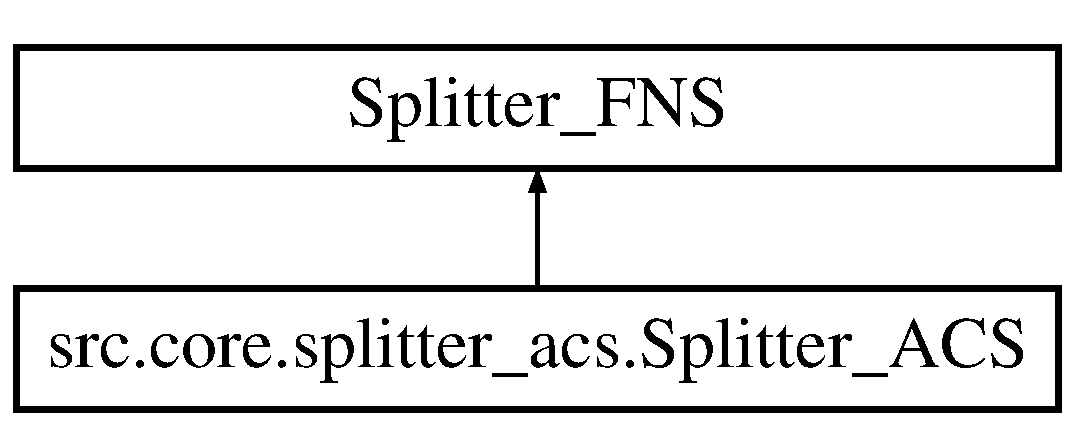
\includegraphics[height=2.000000cm]{classsrc_1_1core_1_1splitter__acs_1_1Splitter__ACS}
\end{center}
\end{figure}
\subsection*{Public Member Functions}
\begin{DoxyCompactItemize}
\item 
def \hyperlink{classsrc_1_1core_1_1splitter__acs_1_1Splitter__ACS_ac23b604c4f1d63f291a142e47ea71471}{\+\_\+\+\_\+init\+\_\+\+\_\+} (self)
\item 
def \hyperlink{classsrc_1_1core_1_1splitter__acs_1_1Splitter__ACS_a0f940285451c895e56e8fdf00d0473ef}{insert\+\_\+peer} (self, peer)
\item 
def \hyperlink{classsrc_1_1core_1_1splitter__acs_1_1Splitter__ACS_ad98bef3ff83336097388e65abed39d07}{increment\+\_\+unsupportivity\+\_\+of\+\_\+peer} (self, peer)
\item 
def \hyperlink{classsrc_1_1core_1_1splitter__acs_1_1Splitter__ACS_a3c5df7e863da1ed06bdd5cf0281ced87}{remove\+\_\+peer} (self, peer)
\item 
def \hyperlink{classsrc_1_1core_1_1splitter__acs_1_1Splitter__ACS_a9d6818ebb334e4cb90b427f9d2e825e6}{reset\+\_\+counters} (self)
\item 
def \hyperlink{classsrc_1_1core_1_1splitter__acs_1_1Splitter__ACS_a810084dae6063307d4c9585958899c9b}{send\+\_\+chunk} (self, chunk, peer)
\item 
def \hyperlink{classsrc_1_1core_1_1splitter__acs_1_1Splitter__ACS_aa16e0352e28e26f4969ffc91b8e4ac80}{compute\+\_\+next\+\_\+peer\+\_\+number} (self, peer)
\end{DoxyCompactItemize}
\subsection*{Public Attributes}
\begin{DoxyCompactItemize}
\item 
\hyperlink{classsrc_1_1core_1_1splitter__acs_1_1Splitter__ACS_af9a82fe476fdc7bf419cfa099a839350}{period}
\item 
\hyperlink{classsrc_1_1core_1_1splitter__acs_1_1Splitter__ACS_a1bfd9ecd4c14ccbe48ec6055f1cfc45f}{period\+\_\+counter}
\item 
\hyperlink{classsrc_1_1core_1_1splitter__acs_1_1Splitter__ACS_acfed35d908382e1e320195b10cddc844}{number\+\_\+of\+\_\+sent\+\_\+chunks\+\_\+per\+\_\+peer}
\item 
\hyperlink{classsrc_1_1core_1_1splitter__acs_1_1Splitter__ACS_ab20eaa4229c6999c79809725e35a72aa}{peer\+\_\+number}
\end{DoxyCompactItemize}


\subsection{Constructor \& Destructor Documentation}
\hypertarget{classsrc_1_1core_1_1splitter__acs_1_1Splitter__ACS_ac23b604c4f1d63f291a142e47ea71471}{}\index{src\+::core\+::splitter\+\_\+acs\+::\+Splitter\+\_\+\+A\+C\+S@{src\+::core\+::splitter\+\_\+acs\+::\+Splitter\+\_\+\+A\+C\+S}!\+\_\+\+\_\+init\+\_\+\+\_\+@{\+\_\+\+\_\+init\+\_\+\+\_\+}}
\index{\+\_\+\+\_\+init\+\_\+\+\_\+@{\+\_\+\+\_\+init\+\_\+\+\_\+}!src\+::core\+::splitter\+\_\+acs\+::\+Splitter\+\_\+\+A\+C\+S@{src\+::core\+::splitter\+\_\+acs\+::\+Splitter\+\_\+\+A\+C\+S}}
\subsubsection[{\+\_\+\+\_\+init\+\_\+\+\_\+}]{\setlength{\rightskip}{0pt plus 5cm}def src.\+core.\+splitter\+\_\+acs.\+Splitter\+\_\+\+A\+C\+S.\+\_\+\+\_\+init\+\_\+\+\_\+ (
\begin{DoxyParamCaption}
\item[{}]{self}
\end{DoxyParamCaption}
)}\label{classsrc_1_1core_1_1splitter__acs_1_1Splitter__ACS_ac23b604c4f1d63f291a142e47ea71471}


\subsection{Member Function Documentation}
\hypertarget{classsrc_1_1core_1_1splitter__acs_1_1Splitter__ACS_aa16e0352e28e26f4969ffc91b8e4ac80}{}\index{src\+::core\+::splitter\+\_\+acs\+::\+Splitter\+\_\+\+A\+C\+S@{src\+::core\+::splitter\+\_\+acs\+::\+Splitter\+\_\+\+A\+C\+S}!compute\+\_\+next\+\_\+peer\+\_\+number@{compute\+\_\+next\+\_\+peer\+\_\+number}}
\index{compute\+\_\+next\+\_\+peer\+\_\+number@{compute\+\_\+next\+\_\+peer\+\_\+number}!src\+::core\+::splitter\+\_\+acs\+::\+Splitter\+\_\+\+A\+C\+S@{src\+::core\+::splitter\+\_\+acs\+::\+Splitter\+\_\+\+A\+C\+S}}
\subsubsection[{compute\+\_\+next\+\_\+peer\+\_\+number}]{\setlength{\rightskip}{0pt plus 5cm}def src.\+core.\+splitter\+\_\+acs.\+Splitter\+\_\+\+A\+C\+S.\+compute\+\_\+next\+\_\+peer\+\_\+number (
\begin{DoxyParamCaption}
\item[{}]{self, }
\item[{}]{peer}
\end{DoxyParamCaption}
)}\label{classsrc_1_1core_1_1splitter__acs_1_1Splitter__ACS_aa16e0352e28e26f4969ffc91b8e4ac80}
\hypertarget{classsrc_1_1core_1_1splitter__acs_1_1Splitter__ACS_ad98bef3ff83336097388e65abed39d07}{}\index{src\+::core\+::splitter\+\_\+acs\+::\+Splitter\+\_\+\+A\+C\+S@{src\+::core\+::splitter\+\_\+acs\+::\+Splitter\+\_\+\+A\+C\+S}!increment\+\_\+unsupportivity\+\_\+of\+\_\+peer@{increment\+\_\+unsupportivity\+\_\+of\+\_\+peer}}
\index{increment\+\_\+unsupportivity\+\_\+of\+\_\+peer@{increment\+\_\+unsupportivity\+\_\+of\+\_\+peer}!src\+::core\+::splitter\+\_\+acs\+::\+Splitter\+\_\+\+A\+C\+S@{src\+::core\+::splitter\+\_\+acs\+::\+Splitter\+\_\+\+A\+C\+S}}
\subsubsection[{increment\+\_\+unsupportivity\+\_\+of\+\_\+peer}]{\setlength{\rightskip}{0pt plus 5cm}def src.\+core.\+splitter\+\_\+acs.\+Splitter\+\_\+\+A\+C\+S.\+increment\+\_\+unsupportivity\+\_\+of\+\_\+peer (
\begin{DoxyParamCaption}
\item[{}]{self, }
\item[{}]{peer}
\end{DoxyParamCaption}
)}\label{classsrc_1_1core_1_1splitter__acs_1_1Splitter__ACS_ad98bef3ff83336097388e65abed39d07}
\hypertarget{classsrc_1_1core_1_1splitter__acs_1_1Splitter__ACS_a0f940285451c895e56e8fdf00d0473ef}{}\index{src\+::core\+::splitter\+\_\+acs\+::\+Splitter\+\_\+\+A\+C\+S@{src\+::core\+::splitter\+\_\+acs\+::\+Splitter\+\_\+\+A\+C\+S}!insert\+\_\+peer@{insert\+\_\+peer}}
\index{insert\+\_\+peer@{insert\+\_\+peer}!src\+::core\+::splitter\+\_\+acs\+::\+Splitter\+\_\+\+A\+C\+S@{src\+::core\+::splitter\+\_\+acs\+::\+Splitter\+\_\+\+A\+C\+S}}
\subsubsection[{insert\+\_\+peer}]{\setlength{\rightskip}{0pt plus 5cm}def src.\+core.\+splitter\+\_\+acs.\+Splitter\+\_\+\+A\+C\+S.\+insert\+\_\+peer (
\begin{DoxyParamCaption}
\item[{}]{self, }
\item[{}]{peer}
\end{DoxyParamCaption}
)}\label{classsrc_1_1core_1_1splitter__acs_1_1Splitter__ACS_a0f940285451c895e56e8fdf00d0473ef}
\hypertarget{classsrc_1_1core_1_1splitter__acs_1_1Splitter__ACS_a3c5df7e863da1ed06bdd5cf0281ced87}{}\index{src\+::core\+::splitter\+\_\+acs\+::\+Splitter\+\_\+\+A\+C\+S@{src\+::core\+::splitter\+\_\+acs\+::\+Splitter\+\_\+\+A\+C\+S}!remove\+\_\+peer@{remove\+\_\+peer}}
\index{remove\+\_\+peer@{remove\+\_\+peer}!src\+::core\+::splitter\+\_\+acs\+::\+Splitter\+\_\+\+A\+C\+S@{src\+::core\+::splitter\+\_\+acs\+::\+Splitter\+\_\+\+A\+C\+S}}
\subsubsection[{remove\+\_\+peer}]{\setlength{\rightskip}{0pt plus 5cm}def src.\+core.\+splitter\+\_\+acs.\+Splitter\+\_\+\+A\+C\+S.\+remove\+\_\+peer (
\begin{DoxyParamCaption}
\item[{}]{self, }
\item[{}]{peer}
\end{DoxyParamCaption}
)}\label{classsrc_1_1core_1_1splitter__acs_1_1Splitter__ACS_a3c5df7e863da1ed06bdd5cf0281ced87}
\hypertarget{classsrc_1_1core_1_1splitter__acs_1_1Splitter__ACS_a9d6818ebb334e4cb90b427f9d2e825e6}{}\index{src\+::core\+::splitter\+\_\+acs\+::\+Splitter\+\_\+\+A\+C\+S@{src\+::core\+::splitter\+\_\+acs\+::\+Splitter\+\_\+\+A\+C\+S}!reset\+\_\+counters@{reset\+\_\+counters}}
\index{reset\+\_\+counters@{reset\+\_\+counters}!src\+::core\+::splitter\+\_\+acs\+::\+Splitter\+\_\+\+A\+C\+S@{src\+::core\+::splitter\+\_\+acs\+::\+Splitter\+\_\+\+A\+C\+S}}
\subsubsection[{reset\+\_\+counters}]{\setlength{\rightskip}{0pt plus 5cm}def src.\+core.\+splitter\+\_\+acs.\+Splitter\+\_\+\+A\+C\+S.\+reset\+\_\+counters (
\begin{DoxyParamCaption}
\item[{}]{self}
\end{DoxyParamCaption}
)}\label{classsrc_1_1core_1_1splitter__acs_1_1Splitter__ACS_a9d6818ebb334e4cb90b427f9d2e825e6}
\hypertarget{classsrc_1_1core_1_1splitter__acs_1_1Splitter__ACS_a810084dae6063307d4c9585958899c9b}{}\index{src\+::core\+::splitter\+\_\+acs\+::\+Splitter\+\_\+\+A\+C\+S@{src\+::core\+::splitter\+\_\+acs\+::\+Splitter\+\_\+\+A\+C\+S}!send\+\_\+chunk@{send\+\_\+chunk}}
\index{send\+\_\+chunk@{send\+\_\+chunk}!src\+::core\+::splitter\+\_\+acs\+::\+Splitter\+\_\+\+A\+C\+S@{src\+::core\+::splitter\+\_\+acs\+::\+Splitter\+\_\+\+A\+C\+S}}
\subsubsection[{send\+\_\+chunk}]{\setlength{\rightskip}{0pt plus 5cm}def src.\+core.\+splitter\+\_\+acs.\+Splitter\+\_\+\+A\+C\+S.\+send\+\_\+chunk (
\begin{DoxyParamCaption}
\item[{}]{self, }
\item[{}]{chunk, }
\item[{}]{peer}
\end{DoxyParamCaption}
)}\label{classsrc_1_1core_1_1splitter__acs_1_1Splitter__ACS_a810084dae6063307d4c9585958899c9b}


\subsection{Member Data Documentation}
\hypertarget{classsrc_1_1core_1_1splitter__acs_1_1Splitter__ACS_acfed35d908382e1e320195b10cddc844}{}\index{src\+::core\+::splitter\+\_\+acs\+::\+Splitter\+\_\+\+A\+C\+S@{src\+::core\+::splitter\+\_\+acs\+::\+Splitter\+\_\+\+A\+C\+S}!number\+\_\+of\+\_\+sent\+\_\+chunks\+\_\+per\+\_\+peer@{number\+\_\+of\+\_\+sent\+\_\+chunks\+\_\+per\+\_\+peer}}
\index{number\+\_\+of\+\_\+sent\+\_\+chunks\+\_\+per\+\_\+peer@{number\+\_\+of\+\_\+sent\+\_\+chunks\+\_\+per\+\_\+peer}!src\+::core\+::splitter\+\_\+acs\+::\+Splitter\+\_\+\+A\+C\+S@{src\+::core\+::splitter\+\_\+acs\+::\+Splitter\+\_\+\+A\+C\+S}}
\subsubsection[{number\+\_\+of\+\_\+sent\+\_\+chunks\+\_\+per\+\_\+peer}]{\setlength{\rightskip}{0pt plus 5cm}src.\+core.\+splitter\+\_\+acs.\+Splitter\+\_\+\+A\+C\+S.\+number\+\_\+of\+\_\+sent\+\_\+chunks\+\_\+per\+\_\+peer}\label{classsrc_1_1core_1_1splitter__acs_1_1Splitter__ACS_acfed35d908382e1e320195b10cddc844}
\hypertarget{classsrc_1_1core_1_1splitter__acs_1_1Splitter__ACS_ab20eaa4229c6999c79809725e35a72aa}{}\index{src\+::core\+::splitter\+\_\+acs\+::\+Splitter\+\_\+\+A\+C\+S@{src\+::core\+::splitter\+\_\+acs\+::\+Splitter\+\_\+\+A\+C\+S}!peer\+\_\+number@{peer\+\_\+number}}
\index{peer\+\_\+number@{peer\+\_\+number}!src\+::core\+::splitter\+\_\+acs\+::\+Splitter\+\_\+\+A\+C\+S@{src\+::core\+::splitter\+\_\+acs\+::\+Splitter\+\_\+\+A\+C\+S}}
\subsubsection[{peer\+\_\+number}]{\setlength{\rightskip}{0pt plus 5cm}src.\+core.\+splitter\+\_\+acs.\+Splitter\+\_\+\+A\+C\+S.\+peer\+\_\+number}\label{classsrc_1_1core_1_1splitter__acs_1_1Splitter__ACS_ab20eaa4229c6999c79809725e35a72aa}
\hypertarget{classsrc_1_1core_1_1splitter__acs_1_1Splitter__ACS_af9a82fe476fdc7bf419cfa099a839350}{}\index{src\+::core\+::splitter\+\_\+acs\+::\+Splitter\+\_\+\+A\+C\+S@{src\+::core\+::splitter\+\_\+acs\+::\+Splitter\+\_\+\+A\+C\+S}!period@{period}}
\index{period@{period}!src\+::core\+::splitter\+\_\+acs\+::\+Splitter\+\_\+\+A\+C\+S@{src\+::core\+::splitter\+\_\+acs\+::\+Splitter\+\_\+\+A\+C\+S}}
\subsubsection[{period}]{\setlength{\rightskip}{0pt plus 5cm}src.\+core.\+splitter\+\_\+acs.\+Splitter\+\_\+\+A\+C\+S.\+period}\label{classsrc_1_1core_1_1splitter__acs_1_1Splitter__ACS_af9a82fe476fdc7bf419cfa099a839350}
\hypertarget{classsrc_1_1core_1_1splitter__acs_1_1Splitter__ACS_a1bfd9ecd4c14ccbe48ec6055f1cfc45f}{}\index{src\+::core\+::splitter\+\_\+acs\+::\+Splitter\+\_\+\+A\+C\+S@{src\+::core\+::splitter\+\_\+acs\+::\+Splitter\+\_\+\+A\+C\+S}!period\+\_\+counter@{period\+\_\+counter}}
\index{period\+\_\+counter@{period\+\_\+counter}!src\+::core\+::splitter\+\_\+acs\+::\+Splitter\+\_\+\+A\+C\+S@{src\+::core\+::splitter\+\_\+acs\+::\+Splitter\+\_\+\+A\+C\+S}}
\subsubsection[{period\+\_\+counter}]{\setlength{\rightskip}{0pt plus 5cm}src.\+core.\+splitter\+\_\+acs.\+Splitter\+\_\+\+A\+C\+S.\+period\+\_\+counter}\label{classsrc_1_1core_1_1splitter__acs_1_1Splitter__ACS_a1bfd9ecd4c14ccbe48ec6055f1cfc45f}


The documentation for this class was generated from the following file\+:\begin{DoxyCompactItemize}
\item 
src/core/\hyperlink{splitter__acs_8py}{splitter\+\_\+acs.\+py}\end{DoxyCompactItemize}

\hypertarget{classsrc_1_1core_1_1splitter__dbs_1_1Splitter__DBS}{}\section{src.\+core.\+splitter\+\_\+dbs.\+Splitter\+\_\+\+D\+B\+S Class Reference}
\label{classsrc_1_1core_1_1splitter__dbs_1_1Splitter__DBS}\index{src.\+core.\+splitter\+\_\+dbs.\+Splitter\+\_\+\+D\+B\+S@{src.\+core.\+splitter\+\_\+dbs.\+Splitter\+\_\+\+D\+B\+S}}
Inheritance diagram for src.\+core.\+splitter\+\_\+dbs.\+Splitter\+\_\+\+D\+B\+S\+:\begin{figure}[H]
\begin{center}
\leavevmode
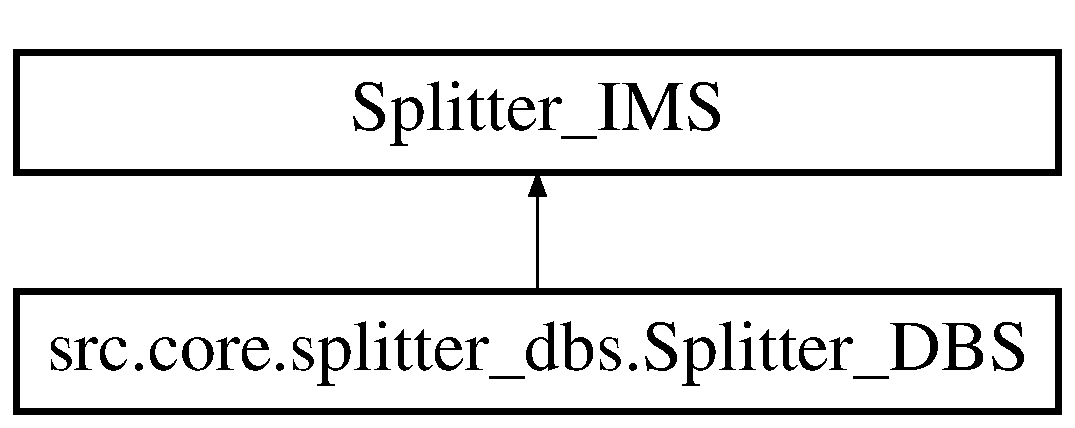
\includegraphics[height=2.000000cm]{classsrc_1_1core_1_1splitter__dbs_1_1Splitter__DBS}
\end{center}
\end{figure}
\subsection*{Public Member Functions}
\begin{DoxyCompactItemize}
\item 
def \hyperlink{classsrc_1_1core_1_1splitter__dbs_1_1Splitter__DBS_a125ba814f93efe1c5f0e43ba9969307e}{\+\_\+\+\_\+init\+\_\+\+\_\+} (self)
\item 
def \hyperlink{classsrc_1_1core_1_1splitter__dbs_1_1Splitter__DBS_abec8f0d525b4a0e226c20faab6999098}{say\+\_\+goodbye} (self, node, sock)
\item 
def \hyperlink{classsrc_1_1core_1_1splitter__dbs_1_1Splitter__DBS_a6c48f8c160861a802e48cc5fbfd5a8c0}{send\+\_\+the\+\_\+list\+\_\+size} (self, peer\+\_\+serve\+\_\+socket)
\item 
def \hyperlink{classsrc_1_1core_1_1splitter__dbs_1_1Splitter__DBS_a3bc94592bc0da6369a4dcab306f2ea52}{send\+\_\+the\+\_\+list\+\_\+of\+\_\+peers} (self, peer\+\_\+serve\+\_\+socket)
\item 
def \hyperlink{classsrc_1_1core_1_1splitter__dbs_1_1Splitter__DBS_ad1f00dcc5c5c0b13b6c0d246903d4542}{send\+\_\+the\+\_\+peer\+\_\+endpoint} (self, peer\+\_\+serve\+\_\+socket)
\item 
def \hyperlink{classsrc_1_1core_1_1splitter__dbs_1_1Splitter__DBS_af7c47014ad636ac10bce62cba7fd88e8}{send\+\_\+configuration} (self, sock)
\item 
def \hyperlink{classsrc_1_1core_1_1splitter__dbs_1_1Splitter__DBS_aca9ff707e7cc0a9a75396fdaf7c77bbb}{insert\+\_\+peer} (self, peer)
\item 
def \hyperlink{classsrc_1_1core_1_1splitter__dbs_1_1Splitter__DBS_a26eccfb34c0b1b506f1bb83d194fc6d3}{handle\+\_\+a\+\_\+peer\+\_\+arrival} (self, connection)
\item 
def \hyperlink{classsrc_1_1core_1_1splitter__dbs_1_1Splitter__DBS_a501a9d297e2ed2d776e4c087ab3c7622}{receive\+\_\+message} (self)
\item 
def \hyperlink{classsrc_1_1core_1_1splitter__dbs_1_1Splitter__DBS_a4dc67f4a285c696bcccf8f8b1e5f7444}{get\+\_\+lost\+\_\+chunk\+\_\+number} (self, message)
\item 
def \hyperlink{classsrc_1_1core_1_1splitter__dbs_1_1Splitter__DBS_afd4db338ba62ab8de3d7d0ae3b9cd76f}{get\+\_\+losser} (self, lost\+\_\+chunk\+\_\+number)
\item 
def \hyperlink{classsrc_1_1core_1_1splitter__dbs_1_1Splitter__DBS_a55e2b2b3648d428c6188a9dd54746adf}{remove\+\_\+peer} (self, peer)
\item 
def \hyperlink{classsrc_1_1core_1_1splitter__dbs_1_1Splitter__DBS_adefda40274ae5e75d57b67907ad03bb7}{increment\+\_\+unsupportivity\+\_\+of\+\_\+peer} (self, peer)
\item 
def \hyperlink{classsrc_1_1core_1_1splitter__dbs_1_1Splitter__DBS_acf0da7b0b7251915736377891ca0c12f}{process\+\_\+lost\+\_\+chunk} (self, lost\+\_\+chunk\+\_\+number, sender)
\item 
def \hyperlink{classsrc_1_1core_1_1splitter__dbs_1_1Splitter__DBS_aa21e8c9c535770b9ce138946849c4bf6}{process\+\_\+goodbye} (self, peer)
\item 
def \hyperlink{classsrc_1_1core_1_1splitter__dbs_1_1Splitter__DBS_a34d1a49ab596722417a528ff9d6c82f9}{moderate\+\_\+the\+\_\+team} (self)
\item 
def \hyperlink{classsrc_1_1core_1_1splitter__dbs_1_1Splitter__DBS_a305e32f518f64e76b8cb71cb4cbc9259}{setup\+\_\+team\+\_\+socket} (self)
\item 
def \hyperlink{classsrc_1_1core_1_1splitter__dbs_1_1Splitter__DBS_a7482a1adb2c1779f4187fb9550a4f4f4}{reset\+\_\+counters} (self)
\item 
def \hyperlink{classsrc_1_1core_1_1splitter__dbs_1_1Splitter__DBS_a34e493f0c70253f0a7566526d170655b}{reset\+\_\+counters\+\_\+thread} (self)
\item 
def \hyperlink{classsrc_1_1core_1_1splitter__dbs_1_1Splitter__DBS_a9bc2503fabf5e82372a2cd0ad7ca295e}{compute\+\_\+next\+\_\+peer\+\_\+number} (self, peer)
\item 
def \hyperlink{classsrc_1_1core_1_1splitter__dbs_1_1Splitter__DBS_a9ef9d1f2eb54fa6bc5fd2a5347d90787}{run} (self)
\end{DoxyCompactItemize}
\subsection*{Public Attributes}
\begin{DoxyCompactItemize}
\item 
\hyperlink{classsrc_1_1core_1_1splitter__dbs_1_1Splitter__DBS_a016cab7dccefdeb3ddfb8c39e34be195}{peer\+\_\+number}
\item 
\hyperlink{classsrc_1_1core_1_1splitter__dbs_1_1Splitter__DBS_a5b9e5b4e0fedea431b5b097794bd8e9a}{peer\+\_\+list}
\item 
\hyperlink{classsrc_1_1core_1_1splitter__dbs_1_1Splitter__DBS_ae679c86a9ae870b8968c11d49054f695}{destination\+\_\+of\+\_\+chunk}
\item 
\hyperlink{classsrc_1_1core_1_1splitter__dbs_1_1Splitter__DBS_a239a850a857f3b55d5aa4f49140d4e87}{losses}
\item 
\hyperlink{classsrc_1_1core_1_1splitter__dbs_1_1Splitter__DBS_acd50eb2fee3c9691cd631f4eb293d581}{team\+\_\+socket}
\item 
\hyperlink{classsrc_1_1core_1_1splitter__dbs_1_1Splitter__DBS_a482922e27a35771453628c3aa47ce7cd}{chunk\+\_\+number}
\end{DoxyCompactItemize}
\subsection*{Static Public Attributes}
\begin{DoxyCompactItemize}
\item 
int \hyperlink{classsrc_1_1core_1_1splitter__dbs_1_1Splitter__DBS_adedee80ea32e692f23f8af49e12de74e}{M\+A\+X\+\_\+\+C\+H\+U\+N\+K\+\_\+\+L\+O\+S\+S} = 32
\item 
string \hyperlink{classsrc_1_1core_1_1splitter__dbs_1_1Splitter__DBS_a201af74a1173c2738168ee21350b2af7}{M\+C\+A\+S\+T\+\_\+\+A\+D\+D\+R} = \char`\"{}0.\+0.\+0.\+0\char`\"{}
\end{DoxyCompactItemize}


\subsection{Constructor \& Destructor Documentation}
\hypertarget{classsrc_1_1core_1_1splitter__dbs_1_1Splitter__DBS_a125ba814f93efe1c5f0e43ba9969307e}{}\index{src\+::core\+::splitter\+\_\+dbs\+::\+Splitter\+\_\+\+D\+B\+S@{src\+::core\+::splitter\+\_\+dbs\+::\+Splitter\+\_\+\+D\+B\+S}!\+\_\+\+\_\+init\+\_\+\+\_\+@{\+\_\+\+\_\+init\+\_\+\+\_\+}}
\index{\+\_\+\+\_\+init\+\_\+\+\_\+@{\+\_\+\+\_\+init\+\_\+\+\_\+}!src\+::core\+::splitter\+\_\+dbs\+::\+Splitter\+\_\+\+D\+B\+S@{src\+::core\+::splitter\+\_\+dbs\+::\+Splitter\+\_\+\+D\+B\+S}}
\subsubsection[{\+\_\+\+\_\+init\+\_\+\+\_\+}]{\setlength{\rightskip}{0pt plus 5cm}def src.\+core.\+splitter\+\_\+dbs.\+Splitter\+\_\+\+D\+B\+S.\+\_\+\+\_\+init\+\_\+\+\_\+ (
\begin{DoxyParamCaption}
\item[{}]{self}
\end{DoxyParamCaption}
)}\label{classsrc_1_1core_1_1splitter__dbs_1_1Splitter__DBS_a125ba814f93efe1c5f0e43ba9969307e}


\subsection{Member Function Documentation}
\hypertarget{classsrc_1_1core_1_1splitter__dbs_1_1Splitter__DBS_a9bc2503fabf5e82372a2cd0ad7ca295e}{}\index{src\+::core\+::splitter\+\_\+dbs\+::\+Splitter\+\_\+\+D\+B\+S@{src\+::core\+::splitter\+\_\+dbs\+::\+Splitter\+\_\+\+D\+B\+S}!compute\+\_\+next\+\_\+peer\+\_\+number@{compute\+\_\+next\+\_\+peer\+\_\+number}}
\index{compute\+\_\+next\+\_\+peer\+\_\+number@{compute\+\_\+next\+\_\+peer\+\_\+number}!src\+::core\+::splitter\+\_\+dbs\+::\+Splitter\+\_\+\+D\+B\+S@{src\+::core\+::splitter\+\_\+dbs\+::\+Splitter\+\_\+\+D\+B\+S}}
\subsubsection[{compute\+\_\+next\+\_\+peer\+\_\+number}]{\setlength{\rightskip}{0pt plus 5cm}def src.\+core.\+splitter\+\_\+dbs.\+Splitter\+\_\+\+D\+B\+S.\+compute\+\_\+next\+\_\+peer\+\_\+number (
\begin{DoxyParamCaption}
\item[{}]{self, }
\item[{}]{peer}
\end{DoxyParamCaption}
)}\label{classsrc_1_1core_1_1splitter__dbs_1_1Splitter__DBS_a9bc2503fabf5e82372a2cd0ad7ca295e}
\hypertarget{classsrc_1_1core_1_1splitter__dbs_1_1Splitter__DBS_afd4db338ba62ab8de3d7d0ae3b9cd76f}{}\index{src\+::core\+::splitter\+\_\+dbs\+::\+Splitter\+\_\+\+D\+B\+S@{src\+::core\+::splitter\+\_\+dbs\+::\+Splitter\+\_\+\+D\+B\+S}!get\+\_\+losser@{get\+\_\+losser}}
\index{get\+\_\+losser@{get\+\_\+losser}!src\+::core\+::splitter\+\_\+dbs\+::\+Splitter\+\_\+\+D\+B\+S@{src\+::core\+::splitter\+\_\+dbs\+::\+Splitter\+\_\+\+D\+B\+S}}
\subsubsection[{get\+\_\+losser}]{\setlength{\rightskip}{0pt plus 5cm}def src.\+core.\+splitter\+\_\+dbs.\+Splitter\+\_\+\+D\+B\+S.\+get\+\_\+losser (
\begin{DoxyParamCaption}
\item[{}]{self, }
\item[{}]{lost\+\_\+chunk\+\_\+number}
\end{DoxyParamCaption}
)}\label{classsrc_1_1core_1_1splitter__dbs_1_1Splitter__DBS_afd4db338ba62ab8de3d7d0ae3b9cd76f}
\hypertarget{classsrc_1_1core_1_1splitter__dbs_1_1Splitter__DBS_a4dc67f4a285c696bcccf8f8b1e5f7444}{}\index{src\+::core\+::splitter\+\_\+dbs\+::\+Splitter\+\_\+\+D\+B\+S@{src\+::core\+::splitter\+\_\+dbs\+::\+Splitter\+\_\+\+D\+B\+S}!get\+\_\+lost\+\_\+chunk\+\_\+number@{get\+\_\+lost\+\_\+chunk\+\_\+number}}
\index{get\+\_\+lost\+\_\+chunk\+\_\+number@{get\+\_\+lost\+\_\+chunk\+\_\+number}!src\+::core\+::splitter\+\_\+dbs\+::\+Splitter\+\_\+\+D\+B\+S@{src\+::core\+::splitter\+\_\+dbs\+::\+Splitter\+\_\+\+D\+B\+S}}
\subsubsection[{get\+\_\+lost\+\_\+chunk\+\_\+number}]{\setlength{\rightskip}{0pt plus 5cm}def src.\+core.\+splitter\+\_\+dbs.\+Splitter\+\_\+\+D\+B\+S.\+get\+\_\+lost\+\_\+chunk\+\_\+number (
\begin{DoxyParamCaption}
\item[{}]{self, }
\item[{}]{message}
\end{DoxyParamCaption}
)}\label{classsrc_1_1core_1_1splitter__dbs_1_1Splitter__DBS_a4dc67f4a285c696bcccf8f8b1e5f7444}
\hypertarget{classsrc_1_1core_1_1splitter__dbs_1_1Splitter__DBS_a26eccfb34c0b1b506f1bb83d194fc6d3}{}\index{src\+::core\+::splitter\+\_\+dbs\+::\+Splitter\+\_\+\+D\+B\+S@{src\+::core\+::splitter\+\_\+dbs\+::\+Splitter\+\_\+\+D\+B\+S}!handle\+\_\+a\+\_\+peer\+\_\+arrival@{handle\+\_\+a\+\_\+peer\+\_\+arrival}}
\index{handle\+\_\+a\+\_\+peer\+\_\+arrival@{handle\+\_\+a\+\_\+peer\+\_\+arrival}!src\+::core\+::splitter\+\_\+dbs\+::\+Splitter\+\_\+\+D\+B\+S@{src\+::core\+::splitter\+\_\+dbs\+::\+Splitter\+\_\+\+D\+B\+S}}
\subsubsection[{handle\+\_\+a\+\_\+peer\+\_\+arrival}]{\setlength{\rightskip}{0pt plus 5cm}def src.\+core.\+splitter\+\_\+dbs.\+Splitter\+\_\+\+D\+B\+S.\+handle\+\_\+a\+\_\+peer\+\_\+arrival (
\begin{DoxyParamCaption}
\item[{}]{self, }
\item[{}]{connection}
\end{DoxyParamCaption}
)}\label{classsrc_1_1core_1_1splitter__dbs_1_1Splitter__DBS_a26eccfb34c0b1b506f1bb83d194fc6d3}
\hypertarget{classsrc_1_1core_1_1splitter__dbs_1_1Splitter__DBS_adefda40274ae5e75d57b67907ad03bb7}{}\index{src\+::core\+::splitter\+\_\+dbs\+::\+Splitter\+\_\+\+D\+B\+S@{src\+::core\+::splitter\+\_\+dbs\+::\+Splitter\+\_\+\+D\+B\+S}!increment\+\_\+unsupportivity\+\_\+of\+\_\+peer@{increment\+\_\+unsupportivity\+\_\+of\+\_\+peer}}
\index{increment\+\_\+unsupportivity\+\_\+of\+\_\+peer@{increment\+\_\+unsupportivity\+\_\+of\+\_\+peer}!src\+::core\+::splitter\+\_\+dbs\+::\+Splitter\+\_\+\+D\+B\+S@{src\+::core\+::splitter\+\_\+dbs\+::\+Splitter\+\_\+\+D\+B\+S}}
\subsubsection[{increment\+\_\+unsupportivity\+\_\+of\+\_\+peer}]{\setlength{\rightskip}{0pt plus 5cm}def src.\+core.\+splitter\+\_\+dbs.\+Splitter\+\_\+\+D\+B\+S.\+increment\+\_\+unsupportivity\+\_\+of\+\_\+peer (
\begin{DoxyParamCaption}
\item[{}]{self, }
\item[{}]{peer}
\end{DoxyParamCaption}
)}\label{classsrc_1_1core_1_1splitter__dbs_1_1Splitter__DBS_adefda40274ae5e75d57b67907ad03bb7}
\hypertarget{classsrc_1_1core_1_1splitter__dbs_1_1Splitter__DBS_aca9ff707e7cc0a9a75396fdaf7c77bbb}{}\index{src\+::core\+::splitter\+\_\+dbs\+::\+Splitter\+\_\+\+D\+B\+S@{src\+::core\+::splitter\+\_\+dbs\+::\+Splitter\+\_\+\+D\+B\+S}!insert\+\_\+peer@{insert\+\_\+peer}}
\index{insert\+\_\+peer@{insert\+\_\+peer}!src\+::core\+::splitter\+\_\+dbs\+::\+Splitter\+\_\+\+D\+B\+S@{src\+::core\+::splitter\+\_\+dbs\+::\+Splitter\+\_\+\+D\+B\+S}}
\subsubsection[{insert\+\_\+peer}]{\setlength{\rightskip}{0pt plus 5cm}def src.\+core.\+splitter\+\_\+dbs.\+Splitter\+\_\+\+D\+B\+S.\+insert\+\_\+peer (
\begin{DoxyParamCaption}
\item[{}]{self, }
\item[{}]{peer}
\end{DoxyParamCaption}
)}\label{classsrc_1_1core_1_1splitter__dbs_1_1Splitter__DBS_aca9ff707e7cc0a9a75396fdaf7c77bbb}
\hypertarget{classsrc_1_1core_1_1splitter__dbs_1_1Splitter__DBS_a34d1a49ab596722417a528ff9d6c82f9}{}\index{src\+::core\+::splitter\+\_\+dbs\+::\+Splitter\+\_\+\+D\+B\+S@{src\+::core\+::splitter\+\_\+dbs\+::\+Splitter\+\_\+\+D\+B\+S}!moderate\+\_\+the\+\_\+team@{moderate\+\_\+the\+\_\+team}}
\index{moderate\+\_\+the\+\_\+team@{moderate\+\_\+the\+\_\+team}!src\+::core\+::splitter\+\_\+dbs\+::\+Splitter\+\_\+\+D\+B\+S@{src\+::core\+::splitter\+\_\+dbs\+::\+Splitter\+\_\+\+D\+B\+S}}
\subsubsection[{moderate\+\_\+the\+\_\+team}]{\setlength{\rightskip}{0pt plus 5cm}def src.\+core.\+splitter\+\_\+dbs.\+Splitter\+\_\+\+D\+B\+S.\+moderate\+\_\+the\+\_\+team (
\begin{DoxyParamCaption}
\item[{}]{self}
\end{DoxyParamCaption}
)}\label{classsrc_1_1core_1_1splitter__dbs_1_1Splitter__DBS_a34d1a49ab596722417a528ff9d6c82f9}
\hypertarget{classsrc_1_1core_1_1splitter__dbs_1_1Splitter__DBS_aa21e8c9c535770b9ce138946849c4bf6}{}\index{src\+::core\+::splitter\+\_\+dbs\+::\+Splitter\+\_\+\+D\+B\+S@{src\+::core\+::splitter\+\_\+dbs\+::\+Splitter\+\_\+\+D\+B\+S}!process\+\_\+goodbye@{process\+\_\+goodbye}}
\index{process\+\_\+goodbye@{process\+\_\+goodbye}!src\+::core\+::splitter\+\_\+dbs\+::\+Splitter\+\_\+\+D\+B\+S@{src\+::core\+::splitter\+\_\+dbs\+::\+Splitter\+\_\+\+D\+B\+S}}
\subsubsection[{process\+\_\+goodbye}]{\setlength{\rightskip}{0pt plus 5cm}def src.\+core.\+splitter\+\_\+dbs.\+Splitter\+\_\+\+D\+B\+S.\+process\+\_\+goodbye (
\begin{DoxyParamCaption}
\item[{}]{self, }
\item[{}]{peer}
\end{DoxyParamCaption}
)}\label{classsrc_1_1core_1_1splitter__dbs_1_1Splitter__DBS_aa21e8c9c535770b9ce138946849c4bf6}
\hypertarget{classsrc_1_1core_1_1splitter__dbs_1_1Splitter__DBS_acf0da7b0b7251915736377891ca0c12f}{}\index{src\+::core\+::splitter\+\_\+dbs\+::\+Splitter\+\_\+\+D\+B\+S@{src\+::core\+::splitter\+\_\+dbs\+::\+Splitter\+\_\+\+D\+B\+S}!process\+\_\+lost\+\_\+chunk@{process\+\_\+lost\+\_\+chunk}}
\index{process\+\_\+lost\+\_\+chunk@{process\+\_\+lost\+\_\+chunk}!src\+::core\+::splitter\+\_\+dbs\+::\+Splitter\+\_\+\+D\+B\+S@{src\+::core\+::splitter\+\_\+dbs\+::\+Splitter\+\_\+\+D\+B\+S}}
\subsubsection[{process\+\_\+lost\+\_\+chunk}]{\setlength{\rightskip}{0pt plus 5cm}def src.\+core.\+splitter\+\_\+dbs.\+Splitter\+\_\+\+D\+B\+S.\+process\+\_\+lost\+\_\+chunk (
\begin{DoxyParamCaption}
\item[{}]{self, }
\item[{}]{lost\+\_\+chunk\+\_\+number, }
\item[{}]{sender}
\end{DoxyParamCaption}
)}\label{classsrc_1_1core_1_1splitter__dbs_1_1Splitter__DBS_acf0da7b0b7251915736377891ca0c12f}
\hypertarget{classsrc_1_1core_1_1splitter__dbs_1_1Splitter__DBS_a501a9d297e2ed2d776e4c087ab3c7622}{}\index{src\+::core\+::splitter\+\_\+dbs\+::\+Splitter\+\_\+\+D\+B\+S@{src\+::core\+::splitter\+\_\+dbs\+::\+Splitter\+\_\+\+D\+B\+S}!receive\+\_\+message@{receive\+\_\+message}}
\index{receive\+\_\+message@{receive\+\_\+message}!src\+::core\+::splitter\+\_\+dbs\+::\+Splitter\+\_\+\+D\+B\+S@{src\+::core\+::splitter\+\_\+dbs\+::\+Splitter\+\_\+\+D\+B\+S}}
\subsubsection[{receive\+\_\+message}]{\setlength{\rightskip}{0pt plus 5cm}def src.\+core.\+splitter\+\_\+dbs.\+Splitter\+\_\+\+D\+B\+S.\+receive\+\_\+message (
\begin{DoxyParamCaption}
\item[{}]{self}
\end{DoxyParamCaption}
)}\label{classsrc_1_1core_1_1splitter__dbs_1_1Splitter__DBS_a501a9d297e2ed2d776e4c087ab3c7622}
\hypertarget{classsrc_1_1core_1_1splitter__dbs_1_1Splitter__DBS_a55e2b2b3648d428c6188a9dd54746adf}{}\index{src\+::core\+::splitter\+\_\+dbs\+::\+Splitter\+\_\+\+D\+B\+S@{src\+::core\+::splitter\+\_\+dbs\+::\+Splitter\+\_\+\+D\+B\+S}!remove\+\_\+peer@{remove\+\_\+peer}}
\index{remove\+\_\+peer@{remove\+\_\+peer}!src\+::core\+::splitter\+\_\+dbs\+::\+Splitter\+\_\+\+D\+B\+S@{src\+::core\+::splitter\+\_\+dbs\+::\+Splitter\+\_\+\+D\+B\+S}}
\subsubsection[{remove\+\_\+peer}]{\setlength{\rightskip}{0pt plus 5cm}def src.\+core.\+splitter\+\_\+dbs.\+Splitter\+\_\+\+D\+B\+S.\+remove\+\_\+peer (
\begin{DoxyParamCaption}
\item[{}]{self, }
\item[{}]{peer}
\end{DoxyParamCaption}
)}\label{classsrc_1_1core_1_1splitter__dbs_1_1Splitter__DBS_a55e2b2b3648d428c6188a9dd54746adf}
\hypertarget{classsrc_1_1core_1_1splitter__dbs_1_1Splitter__DBS_a7482a1adb2c1779f4187fb9550a4f4f4}{}\index{src\+::core\+::splitter\+\_\+dbs\+::\+Splitter\+\_\+\+D\+B\+S@{src\+::core\+::splitter\+\_\+dbs\+::\+Splitter\+\_\+\+D\+B\+S}!reset\+\_\+counters@{reset\+\_\+counters}}
\index{reset\+\_\+counters@{reset\+\_\+counters}!src\+::core\+::splitter\+\_\+dbs\+::\+Splitter\+\_\+\+D\+B\+S@{src\+::core\+::splitter\+\_\+dbs\+::\+Splitter\+\_\+\+D\+B\+S}}
\subsubsection[{reset\+\_\+counters}]{\setlength{\rightskip}{0pt plus 5cm}def src.\+core.\+splitter\+\_\+dbs.\+Splitter\+\_\+\+D\+B\+S.\+reset\+\_\+counters (
\begin{DoxyParamCaption}
\item[{}]{self}
\end{DoxyParamCaption}
)}\label{classsrc_1_1core_1_1splitter__dbs_1_1Splitter__DBS_a7482a1adb2c1779f4187fb9550a4f4f4}
\hypertarget{classsrc_1_1core_1_1splitter__dbs_1_1Splitter__DBS_a34e493f0c70253f0a7566526d170655b}{}\index{src\+::core\+::splitter\+\_\+dbs\+::\+Splitter\+\_\+\+D\+B\+S@{src\+::core\+::splitter\+\_\+dbs\+::\+Splitter\+\_\+\+D\+B\+S}!reset\+\_\+counters\+\_\+thread@{reset\+\_\+counters\+\_\+thread}}
\index{reset\+\_\+counters\+\_\+thread@{reset\+\_\+counters\+\_\+thread}!src\+::core\+::splitter\+\_\+dbs\+::\+Splitter\+\_\+\+D\+B\+S@{src\+::core\+::splitter\+\_\+dbs\+::\+Splitter\+\_\+\+D\+B\+S}}
\subsubsection[{reset\+\_\+counters\+\_\+thread}]{\setlength{\rightskip}{0pt plus 5cm}def src.\+core.\+splitter\+\_\+dbs.\+Splitter\+\_\+\+D\+B\+S.\+reset\+\_\+counters\+\_\+thread (
\begin{DoxyParamCaption}
\item[{}]{self}
\end{DoxyParamCaption}
)}\label{classsrc_1_1core_1_1splitter__dbs_1_1Splitter__DBS_a34e493f0c70253f0a7566526d170655b}
\hypertarget{classsrc_1_1core_1_1splitter__dbs_1_1Splitter__DBS_a9ef9d1f2eb54fa6bc5fd2a5347d90787}{}\index{src\+::core\+::splitter\+\_\+dbs\+::\+Splitter\+\_\+\+D\+B\+S@{src\+::core\+::splitter\+\_\+dbs\+::\+Splitter\+\_\+\+D\+B\+S}!run@{run}}
\index{run@{run}!src\+::core\+::splitter\+\_\+dbs\+::\+Splitter\+\_\+\+D\+B\+S@{src\+::core\+::splitter\+\_\+dbs\+::\+Splitter\+\_\+\+D\+B\+S}}
\subsubsection[{run}]{\setlength{\rightskip}{0pt plus 5cm}def src.\+core.\+splitter\+\_\+dbs.\+Splitter\+\_\+\+D\+B\+S.\+run (
\begin{DoxyParamCaption}
\item[{}]{self}
\end{DoxyParamCaption}
)}\label{classsrc_1_1core_1_1splitter__dbs_1_1Splitter__DBS_a9ef9d1f2eb54fa6bc5fd2a5347d90787}
\hypertarget{classsrc_1_1core_1_1splitter__dbs_1_1Splitter__DBS_abec8f0d525b4a0e226c20faab6999098}{}\index{src\+::core\+::splitter\+\_\+dbs\+::\+Splitter\+\_\+\+D\+B\+S@{src\+::core\+::splitter\+\_\+dbs\+::\+Splitter\+\_\+\+D\+B\+S}!say\+\_\+goodbye@{say\+\_\+goodbye}}
\index{say\+\_\+goodbye@{say\+\_\+goodbye}!src\+::core\+::splitter\+\_\+dbs\+::\+Splitter\+\_\+\+D\+B\+S@{src\+::core\+::splitter\+\_\+dbs\+::\+Splitter\+\_\+\+D\+B\+S}}
\subsubsection[{say\+\_\+goodbye}]{\setlength{\rightskip}{0pt plus 5cm}def src.\+core.\+splitter\+\_\+dbs.\+Splitter\+\_\+\+D\+B\+S.\+say\+\_\+goodbye (
\begin{DoxyParamCaption}
\item[{}]{self, }
\item[{}]{node, }
\item[{}]{sock}
\end{DoxyParamCaption}
)}\label{classsrc_1_1core_1_1splitter__dbs_1_1Splitter__DBS_abec8f0d525b4a0e226c20faab6999098}
\hypertarget{classsrc_1_1core_1_1splitter__dbs_1_1Splitter__DBS_af7c47014ad636ac10bce62cba7fd88e8}{}\index{src\+::core\+::splitter\+\_\+dbs\+::\+Splitter\+\_\+\+D\+B\+S@{src\+::core\+::splitter\+\_\+dbs\+::\+Splitter\+\_\+\+D\+B\+S}!send\+\_\+configuration@{send\+\_\+configuration}}
\index{send\+\_\+configuration@{send\+\_\+configuration}!src\+::core\+::splitter\+\_\+dbs\+::\+Splitter\+\_\+\+D\+B\+S@{src\+::core\+::splitter\+\_\+dbs\+::\+Splitter\+\_\+\+D\+B\+S}}
\subsubsection[{send\+\_\+configuration}]{\setlength{\rightskip}{0pt plus 5cm}def src.\+core.\+splitter\+\_\+dbs.\+Splitter\+\_\+\+D\+B\+S.\+send\+\_\+configuration (
\begin{DoxyParamCaption}
\item[{}]{self, }
\item[{}]{sock}
\end{DoxyParamCaption}
)}\label{classsrc_1_1core_1_1splitter__dbs_1_1Splitter__DBS_af7c47014ad636ac10bce62cba7fd88e8}
\hypertarget{classsrc_1_1core_1_1splitter__dbs_1_1Splitter__DBS_a3bc94592bc0da6369a4dcab306f2ea52}{}\index{src\+::core\+::splitter\+\_\+dbs\+::\+Splitter\+\_\+\+D\+B\+S@{src\+::core\+::splitter\+\_\+dbs\+::\+Splitter\+\_\+\+D\+B\+S}!send\+\_\+the\+\_\+list\+\_\+of\+\_\+peers@{send\+\_\+the\+\_\+list\+\_\+of\+\_\+peers}}
\index{send\+\_\+the\+\_\+list\+\_\+of\+\_\+peers@{send\+\_\+the\+\_\+list\+\_\+of\+\_\+peers}!src\+::core\+::splitter\+\_\+dbs\+::\+Splitter\+\_\+\+D\+B\+S@{src\+::core\+::splitter\+\_\+dbs\+::\+Splitter\+\_\+\+D\+B\+S}}
\subsubsection[{send\+\_\+the\+\_\+list\+\_\+of\+\_\+peers}]{\setlength{\rightskip}{0pt plus 5cm}def src.\+core.\+splitter\+\_\+dbs.\+Splitter\+\_\+\+D\+B\+S.\+send\+\_\+the\+\_\+list\+\_\+of\+\_\+peers (
\begin{DoxyParamCaption}
\item[{}]{self, }
\item[{}]{peer\+\_\+serve\+\_\+socket}
\end{DoxyParamCaption}
)}\label{classsrc_1_1core_1_1splitter__dbs_1_1Splitter__DBS_a3bc94592bc0da6369a4dcab306f2ea52}
\hypertarget{classsrc_1_1core_1_1splitter__dbs_1_1Splitter__DBS_a6c48f8c160861a802e48cc5fbfd5a8c0}{}\index{src\+::core\+::splitter\+\_\+dbs\+::\+Splitter\+\_\+\+D\+B\+S@{src\+::core\+::splitter\+\_\+dbs\+::\+Splitter\+\_\+\+D\+B\+S}!send\+\_\+the\+\_\+list\+\_\+size@{send\+\_\+the\+\_\+list\+\_\+size}}
\index{send\+\_\+the\+\_\+list\+\_\+size@{send\+\_\+the\+\_\+list\+\_\+size}!src\+::core\+::splitter\+\_\+dbs\+::\+Splitter\+\_\+\+D\+B\+S@{src\+::core\+::splitter\+\_\+dbs\+::\+Splitter\+\_\+\+D\+B\+S}}
\subsubsection[{send\+\_\+the\+\_\+list\+\_\+size}]{\setlength{\rightskip}{0pt plus 5cm}def src.\+core.\+splitter\+\_\+dbs.\+Splitter\+\_\+\+D\+B\+S.\+send\+\_\+the\+\_\+list\+\_\+size (
\begin{DoxyParamCaption}
\item[{}]{self, }
\item[{}]{peer\+\_\+serve\+\_\+socket}
\end{DoxyParamCaption}
)}\label{classsrc_1_1core_1_1splitter__dbs_1_1Splitter__DBS_a6c48f8c160861a802e48cc5fbfd5a8c0}
\hypertarget{classsrc_1_1core_1_1splitter__dbs_1_1Splitter__DBS_ad1f00dcc5c5c0b13b6c0d246903d4542}{}\index{src\+::core\+::splitter\+\_\+dbs\+::\+Splitter\+\_\+\+D\+B\+S@{src\+::core\+::splitter\+\_\+dbs\+::\+Splitter\+\_\+\+D\+B\+S}!send\+\_\+the\+\_\+peer\+\_\+endpoint@{send\+\_\+the\+\_\+peer\+\_\+endpoint}}
\index{send\+\_\+the\+\_\+peer\+\_\+endpoint@{send\+\_\+the\+\_\+peer\+\_\+endpoint}!src\+::core\+::splitter\+\_\+dbs\+::\+Splitter\+\_\+\+D\+B\+S@{src\+::core\+::splitter\+\_\+dbs\+::\+Splitter\+\_\+\+D\+B\+S}}
\subsubsection[{send\+\_\+the\+\_\+peer\+\_\+endpoint}]{\setlength{\rightskip}{0pt plus 5cm}def src.\+core.\+splitter\+\_\+dbs.\+Splitter\+\_\+\+D\+B\+S.\+send\+\_\+the\+\_\+peer\+\_\+endpoint (
\begin{DoxyParamCaption}
\item[{}]{self, }
\item[{}]{peer\+\_\+serve\+\_\+socket}
\end{DoxyParamCaption}
)}\label{classsrc_1_1core_1_1splitter__dbs_1_1Splitter__DBS_ad1f00dcc5c5c0b13b6c0d246903d4542}
\hypertarget{classsrc_1_1core_1_1splitter__dbs_1_1Splitter__DBS_a305e32f518f64e76b8cb71cb4cbc9259}{}\index{src\+::core\+::splitter\+\_\+dbs\+::\+Splitter\+\_\+\+D\+B\+S@{src\+::core\+::splitter\+\_\+dbs\+::\+Splitter\+\_\+\+D\+B\+S}!setup\+\_\+team\+\_\+socket@{setup\+\_\+team\+\_\+socket}}
\index{setup\+\_\+team\+\_\+socket@{setup\+\_\+team\+\_\+socket}!src\+::core\+::splitter\+\_\+dbs\+::\+Splitter\+\_\+\+D\+B\+S@{src\+::core\+::splitter\+\_\+dbs\+::\+Splitter\+\_\+\+D\+B\+S}}
\subsubsection[{setup\+\_\+team\+\_\+socket}]{\setlength{\rightskip}{0pt plus 5cm}def src.\+core.\+splitter\+\_\+dbs.\+Splitter\+\_\+\+D\+B\+S.\+setup\+\_\+team\+\_\+socket (
\begin{DoxyParamCaption}
\item[{}]{self}
\end{DoxyParamCaption}
)}\label{classsrc_1_1core_1_1splitter__dbs_1_1Splitter__DBS_a305e32f518f64e76b8cb71cb4cbc9259}


\subsection{Member Data Documentation}
\hypertarget{classsrc_1_1core_1_1splitter__dbs_1_1Splitter__DBS_a482922e27a35771453628c3aa47ce7cd}{}\index{src\+::core\+::splitter\+\_\+dbs\+::\+Splitter\+\_\+\+D\+B\+S@{src\+::core\+::splitter\+\_\+dbs\+::\+Splitter\+\_\+\+D\+B\+S}!chunk\+\_\+number@{chunk\+\_\+number}}
\index{chunk\+\_\+number@{chunk\+\_\+number}!src\+::core\+::splitter\+\_\+dbs\+::\+Splitter\+\_\+\+D\+B\+S@{src\+::core\+::splitter\+\_\+dbs\+::\+Splitter\+\_\+\+D\+B\+S}}
\subsubsection[{chunk\+\_\+number}]{\setlength{\rightskip}{0pt plus 5cm}src.\+core.\+splitter\+\_\+dbs.\+Splitter\+\_\+\+D\+B\+S.\+chunk\+\_\+number}\label{classsrc_1_1core_1_1splitter__dbs_1_1Splitter__DBS_a482922e27a35771453628c3aa47ce7cd}
\hypertarget{classsrc_1_1core_1_1splitter__dbs_1_1Splitter__DBS_ae679c86a9ae870b8968c11d49054f695}{}\index{src\+::core\+::splitter\+\_\+dbs\+::\+Splitter\+\_\+\+D\+B\+S@{src\+::core\+::splitter\+\_\+dbs\+::\+Splitter\+\_\+\+D\+B\+S}!destination\+\_\+of\+\_\+chunk@{destination\+\_\+of\+\_\+chunk}}
\index{destination\+\_\+of\+\_\+chunk@{destination\+\_\+of\+\_\+chunk}!src\+::core\+::splitter\+\_\+dbs\+::\+Splitter\+\_\+\+D\+B\+S@{src\+::core\+::splitter\+\_\+dbs\+::\+Splitter\+\_\+\+D\+B\+S}}
\subsubsection[{destination\+\_\+of\+\_\+chunk}]{\setlength{\rightskip}{0pt plus 5cm}src.\+core.\+splitter\+\_\+dbs.\+Splitter\+\_\+\+D\+B\+S.\+destination\+\_\+of\+\_\+chunk}\label{classsrc_1_1core_1_1splitter__dbs_1_1Splitter__DBS_ae679c86a9ae870b8968c11d49054f695}
\hypertarget{classsrc_1_1core_1_1splitter__dbs_1_1Splitter__DBS_a239a850a857f3b55d5aa4f49140d4e87}{}\index{src\+::core\+::splitter\+\_\+dbs\+::\+Splitter\+\_\+\+D\+B\+S@{src\+::core\+::splitter\+\_\+dbs\+::\+Splitter\+\_\+\+D\+B\+S}!losses@{losses}}
\index{losses@{losses}!src\+::core\+::splitter\+\_\+dbs\+::\+Splitter\+\_\+\+D\+B\+S@{src\+::core\+::splitter\+\_\+dbs\+::\+Splitter\+\_\+\+D\+B\+S}}
\subsubsection[{losses}]{\setlength{\rightskip}{0pt plus 5cm}src.\+core.\+splitter\+\_\+dbs.\+Splitter\+\_\+\+D\+B\+S.\+losses}\label{classsrc_1_1core_1_1splitter__dbs_1_1Splitter__DBS_a239a850a857f3b55d5aa4f49140d4e87}
\hypertarget{classsrc_1_1core_1_1splitter__dbs_1_1Splitter__DBS_adedee80ea32e692f23f8af49e12de74e}{}\index{src\+::core\+::splitter\+\_\+dbs\+::\+Splitter\+\_\+\+D\+B\+S@{src\+::core\+::splitter\+\_\+dbs\+::\+Splitter\+\_\+\+D\+B\+S}!M\+A\+X\+\_\+\+C\+H\+U\+N\+K\+\_\+\+L\+O\+S\+S@{M\+A\+X\+\_\+\+C\+H\+U\+N\+K\+\_\+\+L\+O\+S\+S}}
\index{M\+A\+X\+\_\+\+C\+H\+U\+N\+K\+\_\+\+L\+O\+S\+S@{M\+A\+X\+\_\+\+C\+H\+U\+N\+K\+\_\+\+L\+O\+S\+S}!src\+::core\+::splitter\+\_\+dbs\+::\+Splitter\+\_\+\+D\+B\+S@{src\+::core\+::splitter\+\_\+dbs\+::\+Splitter\+\_\+\+D\+B\+S}}
\subsubsection[{M\+A\+X\+\_\+\+C\+H\+U\+N\+K\+\_\+\+L\+O\+S\+S}]{\setlength{\rightskip}{0pt plus 5cm}int src.\+core.\+splitter\+\_\+dbs.\+Splitter\+\_\+\+D\+B\+S.\+M\+A\+X\+\_\+\+C\+H\+U\+N\+K\+\_\+\+L\+O\+S\+S = 32\hspace{0.3cm}{\ttfamily [static]}}\label{classsrc_1_1core_1_1splitter__dbs_1_1Splitter__DBS_adedee80ea32e692f23f8af49e12de74e}
\hypertarget{classsrc_1_1core_1_1splitter__dbs_1_1Splitter__DBS_a201af74a1173c2738168ee21350b2af7}{}\index{src\+::core\+::splitter\+\_\+dbs\+::\+Splitter\+\_\+\+D\+B\+S@{src\+::core\+::splitter\+\_\+dbs\+::\+Splitter\+\_\+\+D\+B\+S}!M\+C\+A\+S\+T\+\_\+\+A\+D\+D\+R@{M\+C\+A\+S\+T\+\_\+\+A\+D\+D\+R}}
\index{M\+C\+A\+S\+T\+\_\+\+A\+D\+D\+R@{M\+C\+A\+S\+T\+\_\+\+A\+D\+D\+R}!src\+::core\+::splitter\+\_\+dbs\+::\+Splitter\+\_\+\+D\+B\+S@{src\+::core\+::splitter\+\_\+dbs\+::\+Splitter\+\_\+\+D\+B\+S}}
\subsubsection[{M\+C\+A\+S\+T\+\_\+\+A\+D\+D\+R}]{\setlength{\rightskip}{0pt plus 5cm}string src.\+core.\+splitter\+\_\+dbs.\+Splitter\+\_\+\+D\+B\+S.\+M\+C\+A\+S\+T\+\_\+\+A\+D\+D\+R = \char`\"{}0.\+0.\+0.\+0\char`\"{}\hspace{0.3cm}{\ttfamily [static]}}\label{classsrc_1_1core_1_1splitter__dbs_1_1Splitter__DBS_a201af74a1173c2738168ee21350b2af7}
\hypertarget{classsrc_1_1core_1_1splitter__dbs_1_1Splitter__DBS_a5b9e5b4e0fedea431b5b097794bd8e9a}{}\index{src\+::core\+::splitter\+\_\+dbs\+::\+Splitter\+\_\+\+D\+B\+S@{src\+::core\+::splitter\+\_\+dbs\+::\+Splitter\+\_\+\+D\+B\+S}!peer\+\_\+list@{peer\+\_\+list}}
\index{peer\+\_\+list@{peer\+\_\+list}!src\+::core\+::splitter\+\_\+dbs\+::\+Splitter\+\_\+\+D\+B\+S@{src\+::core\+::splitter\+\_\+dbs\+::\+Splitter\+\_\+\+D\+B\+S}}
\subsubsection[{peer\+\_\+list}]{\setlength{\rightskip}{0pt plus 5cm}src.\+core.\+splitter\+\_\+dbs.\+Splitter\+\_\+\+D\+B\+S.\+peer\+\_\+list}\label{classsrc_1_1core_1_1splitter__dbs_1_1Splitter__DBS_a5b9e5b4e0fedea431b5b097794bd8e9a}
\hypertarget{classsrc_1_1core_1_1splitter__dbs_1_1Splitter__DBS_a016cab7dccefdeb3ddfb8c39e34be195}{}\index{src\+::core\+::splitter\+\_\+dbs\+::\+Splitter\+\_\+\+D\+B\+S@{src\+::core\+::splitter\+\_\+dbs\+::\+Splitter\+\_\+\+D\+B\+S}!peer\+\_\+number@{peer\+\_\+number}}
\index{peer\+\_\+number@{peer\+\_\+number}!src\+::core\+::splitter\+\_\+dbs\+::\+Splitter\+\_\+\+D\+B\+S@{src\+::core\+::splitter\+\_\+dbs\+::\+Splitter\+\_\+\+D\+B\+S}}
\subsubsection[{peer\+\_\+number}]{\setlength{\rightskip}{0pt plus 5cm}src.\+core.\+splitter\+\_\+dbs.\+Splitter\+\_\+\+D\+B\+S.\+peer\+\_\+number}\label{classsrc_1_1core_1_1splitter__dbs_1_1Splitter__DBS_a016cab7dccefdeb3ddfb8c39e34be195}
\hypertarget{classsrc_1_1core_1_1splitter__dbs_1_1Splitter__DBS_acd50eb2fee3c9691cd631f4eb293d581}{}\index{src\+::core\+::splitter\+\_\+dbs\+::\+Splitter\+\_\+\+D\+B\+S@{src\+::core\+::splitter\+\_\+dbs\+::\+Splitter\+\_\+\+D\+B\+S}!team\+\_\+socket@{team\+\_\+socket}}
\index{team\+\_\+socket@{team\+\_\+socket}!src\+::core\+::splitter\+\_\+dbs\+::\+Splitter\+\_\+\+D\+B\+S@{src\+::core\+::splitter\+\_\+dbs\+::\+Splitter\+\_\+\+D\+B\+S}}
\subsubsection[{team\+\_\+socket}]{\setlength{\rightskip}{0pt plus 5cm}src.\+core.\+splitter\+\_\+dbs.\+Splitter\+\_\+\+D\+B\+S.\+team\+\_\+socket}\label{classsrc_1_1core_1_1splitter__dbs_1_1Splitter__DBS_acd50eb2fee3c9691cd631f4eb293d581}


The documentation for this class was generated from the following file\+:\begin{DoxyCompactItemize}
\item 
src/core/\hyperlink{splitter__dbs_8py}{splitter\+\_\+dbs.\+py}\end{DoxyCompactItemize}

\hypertarget{classsrc_1_1core_1_1splitter__fns_1_1Splitter__FNS}{}\section{src.\+core.\+splitter\+\_\+fns.\+Splitter\+\_\+\+F\+N\+S Class Reference}
\label{classsrc_1_1core_1_1splitter__fns_1_1Splitter__FNS}\index{src.\+core.\+splitter\+\_\+fns.\+Splitter\+\_\+\+F\+N\+S@{src.\+core.\+splitter\+\_\+fns.\+Splitter\+\_\+\+F\+N\+S}}
Inheritance diagram for src.\+core.\+splitter\+\_\+fns.\+Splitter\+\_\+\+F\+N\+S\+:\begin{figure}[H]
\begin{center}
\leavevmode
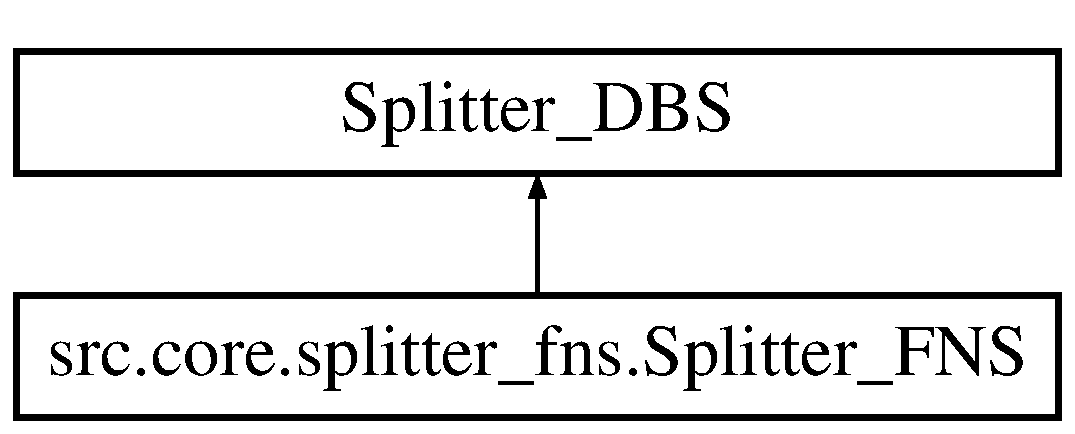
\includegraphics[height=2.000000cm]{classsrc_1_1core_1_1splitter__fns_1_1Splitter__FNS}
\end{center}
\end{figure}
\subsection*{Public Member Functions}
\begin{DoxyCompactItemize}
\item 
def \hyperlink{classsrc_1_1core_1_1splitter__fns_1_1Splitter__FNS_acc04d9ef78298169defea891d66bf42a}{\+\_\+\+\_\+init\+\_\+\+\_\+} (self)
\item 
def \hyperlink{classsrc_1_1core_1_1splitter__fns_1_1Splitter__FNS_a71b079ca9c19ab3e8e15235c3ae17e18}{say\+\_\+goodbye} (self, node, sock)
\item 
def \hyperlink{classsrc_1_1core_1_1splitter__fns_1_1Splitter__FNS_a2ee4b8a8a3f462ba51396cde4af41cc1}{moderate\+\_\+the\+\_\+team} (self)
\end{DoxyCompactItemize}


\subsection{Constructor \& Destructor Documentation}
\hypertarget{classsrc_1_1core_1_1splitter__fns_1_1Splitter__FNS_acc04d9ef78298169defea891d66bf42a}{}\index{src\+::core\+::splitter\+\_\+fns\+::\+Splitter\+\_\+\+F\+N\+S@{src\+::core\+::splitter\+\_\+fns\+::\+Splitter\+\_\+\+F\+N\+S}!\+\_\+\+\_\+init\+\_\+\+\_\+@{\+\_\+\+\_\+init\+\_\+\+\_\+}}
\index{\+\_\+\+\_\+init\+\_\+\+\_\+@{\+\_\+\+\_\+init\+\_\+\+\_\+}!src\+::core\+::splitter\+\_\+fns\+::\+Splitter\+\_\+\+F\+N\+S@{src\+::core\+::splitter\+\_\+fns\+::\+Splitter\+\_\+\+F\+N\+S}}
\subsubsection[{\+\_\+\+\_\+init\+\_\+\+\_\+}]{\setlength{\rightskip}{0pt plus 5cm}def src.\+core.\+splitter\+\_\+fns.\+Splitter\+\_\+\+F\+N\+S.\+\_\+\+\_\+init\+\_\+\+\_\+ (
\begin{DoxyParamCaption}
\item[{}]{self}
\end{DoxyParamCaption}
)}\label{classsrc_1_1core_1_1splitter__fns_1_1Splitter__FNS_acc04d9ef78298169defea891d66bf42a}


\subsection{Member Function Documentation}
\hypertarget{classsrc_1_1core_1_1splitter__fns_1_1Splitter__FNS_a2ee4b8a8a3f462ba51396cde4af41cc1}{}\index{src\+::core\+::splitter\+\_\+fns\+::\+Splitter\+\_\+\+F\+N\+S@{src\+::core\+::splitter\+\_\+fns\+::\+Splitter\+\_\+\+F\+N\+S}!moderate\+\_\+the\+\_\+team@{moderate\+\_\+the\+\_\+team}}
\index{moderate\+\_\+the\+\_\+team@{moderate\+\_\+the\+\_\+team}!src\+::core\+::splitter\+\_\+fns\+::\+Splitter\+\_\+\+F\+N\+S@{src\+::core\+::splitter\+\_\+fns\+::\+Splitter\+\_\+\+F\+N\+S}}
\subsubsection[{moderate\+\_\+the\+\_\+team}]{\setlength{\rightskip}{0pt plus 5cm}def src.\+core.\+splitter\+\_\+fns.\+Splitter\+\_\+\+F\+N\+S.\+moderate\+\_\+the\+\_\+team (
\begin{DoxyParamCaption}
\item[{}]{self}
\end{DoxyParamCaption}
)}\label{classsrc_1_1core_1_1splitter__fns_1_1Splitter__FNS_a2ee4b8a8a3f462ba51396cde4af41cc1}
\hypertarget{classsrc_1_1core_1_1splitter__fns_1_1Splitter__FNS_a71b079ca9c19ab3e8e15235c3ae17e18}{}\index{src\+::core\+::splitter\+\_\+fns\+::\+Splitter\+\_\+\+F\+N\+S@{src\+::core\+::splitter\+\_\+fns\+::\+Splitter\+\_\+\+F\+N\+S}!say\+\_\+goodbye@{say\+\_\+goodbye}}
\index{say\+\_\+goodbye@{say\+\_\+goodbye}!src\+::core\+::splitter\+\_\+fns\+::\+Splitter\+\_\+\+F\+N\+S@{src\+::core\+::splitter\+\_\+fns\+::\+Splitter\+\_\+\+F\+N\+S}}
\subsubsection[{say\+\_\+goodbye}]{\setlength{\rightskip}{0pt plus 5cm}def src.\+core.\+splitter\+\_\+fns.\+Splitter\+\_\+\+F\+N\+S.\+say\+\_\+goodbye (
\begin{DoxyParamCaption}
\item[{}]{self, }
\item[{}]{node, }
\item[{}]{sock}
\end{DoxyParamCaption}
)}\label{classsrc_1_1core_1_1splitter__fns_1_1Splitter__FNS_a71b079ca9c19ab3e8e15235c3ae17e18}


The documentation for this class was generated from the following file\+:\begin{DoxyCompactItemize}
\item 
src/core/\hyperlink{splitter__fns_8py}{splitter\+\_\+fns.\+py}\end{DoxyCompactItemize}

\hypertarget{classsrc_1_1core_1_1splitter__ims_1_1Splitter__IMS}{}\section{src.\+core.\+splitter\+\_\+ims.\+Splitter\+\_\+\+I\+M\+S Class Reference}
\label{classsrc_1_1core_1_1splitter__ims_1_1Splitter__IMS}\index{src.\+core.\+splitter\+\_\+ims.\+Splitter\+\_\+\+I\+M\+S@{src.\+core.\+splitter\+\_\+ims.\+Splitter\+\_\+\+I\+M\+S}}
Inheritance diagram for src.\+core.\+splitter\+\_\+ims.\+Splitter\+\_\+\+I\+M\+S\+:\begin{figure}[H]
\begin{center}
\leavevmode
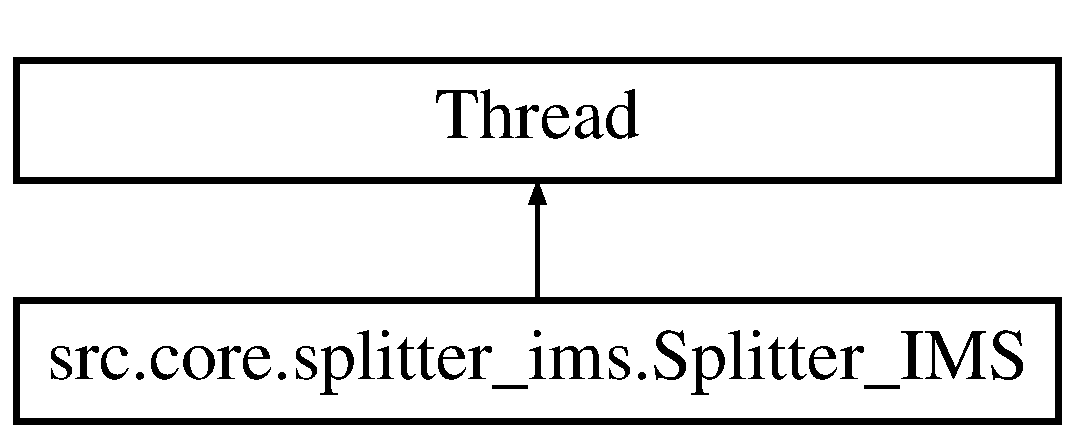
\includegraphics[height=2.000000cm]{classsrc_1_1core_1_1splitter__ims_1_1Splitter__IMS}
\end{center}
\end{figure}
\subsection*{Public Member Functions}
\begin{DoxyCompactItemize}
\item 
def \hyperlink{classsrc_1_1core_1_1splitter__ims_1_1Splitter__IMS_a08e883da468a496050643ed4d3ebe7ec}{\+\_\+\+\_\+init\+\_\+\+\_\+} (self)
\item 
def \hyperlink{classsrc_1_1core_1_1splitter__ims_1_1Splitter__IMS_ab51c45d5be26aa2822185b80320439ca}{send\+\_\+the\+\_\+header} (self, peer\+\_\+serve\+\_\+socket)
\item 
def \hyperlink{classsrc_1_1core_1_1splitter__ims_1_1Splitter__IMS_a2bbdaf55fc7e81e17e8efec91f38788a}{send\+\_\+the\+\_\+buffer\+\_\+size} (self, peer\+\_\+serve\+\_\+socket)
\item 
def \hyperlink{classsrc_1_1core_1_1splitter__ims_1_1Splitter__IMS_a415c0fc4cfe0f025d718be042c5948db}{send\+\_\+the\+\_\+chunk\+\_\+size} (self, peer\+\_\+serve\+\_\+socket)
\item 
def \hyperlink{classsrc_1_1core_1_1splitter__ims_1_1Splitter__IMS_aca4bf65e2da064279b64083d1cb1e404}{send\+\_\+the\+\_\+mcast\+\_\+channel} (self, peer\+\_\+serve\+\_\+socket)
\item 
def \hyperlink{classsrc_1_1core_1_1splitter__ims_1_1Splitter__IMS_a24cfd557424444b9516c11d02938c999}{send\+\_\+the\+\_\+header\+\_\+size} (self, peer\+\_\+serve\+\_\+socket)
\item 
def \hyperlink{classsrc_1_1core_1_1splitter__ims_1_1Splitter__IMS_a8a762b50573ee073ab440d18ff57138c}{send\+\_\+configuration} (self, sock)
\item 
def \hyperlink{classsrc_1_1core_1_1splitter__ims_1_1Splitter__IMS_aff34457cbf46162558aab3a518d7d447}{handle\+\_\+a\+\_\+peer\+\_\+arrival} (self, connection)
\item 
def \hyperlink{classsrc_1_1core_1_1splitter__ims_1_1Splitter__IMS_a64447c571263f0745e61e303c6063d4a}{handle\+\_\+arrivals} (self)
\item 
def \hyperlink{classsrc_1_1core_1_1splitter__ims_1_1Splitter__IMS_a2e49df1eaeb13d3adb01336beed12788}{setup\+\_\+peer\+\_\+connection\+\_\+socket} (self)
\item 
def \hyperlink{classsrc_1_1core_1_1splitter__ims_1_1Splitter__IMS_addc5189d3724bd37c0801a6fc7507c51}{setup\+\_\+team\+\_\+socket} (self)
\item 
def \hyperlink{classsrc_1_1core_1_1splitter__ims_1_1Splitter__IMS_a09234cfb736513eac15319737fc9b141}{request\+\_\+the\+\_\+video\+\_\+from\+\_\+the\+\_\+source} (self)
\item 
def \hyperlink{classsrc_1_1core_1_1splitter__ims_1_1Splitter__IMS_a88b053217e3e4657062043f644fc4c3a}{configure\+\_\+sockets} (self)
\item 
def \hyperlink{classsrc_1_1core_1_1splitter__ims_1_1Splitter__IMS_a1c0b2222975b7e43080337f97904cff1}{load\+\_\+the\+\_\+video\+\_\+header} (self)
\item 
def \hyperlink{classsrc_1_1core_1_1splitter__ims_1_1Splitter__IMS_ab440ec22104aa94f3c436fd93e385262}{receive\+\_\+next\+\_\+chunk} (self)
\item 
def \hyperlink{classsrc_1_1core_1_1splitter__ims_1_1Splitter__IMS_a7890854942cd06c1826351dfe964ace1}{receive\+\_\+chunk} (self)
\item 
def \hyperlink{classsrc_1_1core_1_1splitter__ims_1_1Splitter__IMS_a28035c3e798ff257fd558594a383ea16}{send\+\_\+chunk} (self, message, destine)
\item 
def \hyperlink{classsrc_1_1core_1_1splitter__ims_1_1Splitter__IMS_a7c76103042da1b145ffedb1d7923c741}{receive\+\_\+the\+\_\+header} (self)
\item 
def \hyperlink{classsrc_1_1core_1_1splitter__ims_1_1Splitter__IMS_a2a286adc311b76b64a58b8c87966bd73}{run} (self)
\end{DoxyCompactItemize}
\subsection*{Public Attributes}
\begin{DoxyCompactItemize}
\item 
\hyperlink{classsrc_1_1core_1_1splitter__ims_1_1Splitter__IMS_aa448560064cfec77b4c8b4ff3fb54577}{alive}
\item 
\hyperlink{classsrc_1_1core_1_1splitter__ims_1_1Splitter__IMS_a115d83ea6b9e356af5bfa6e0bf835ffa}{chunk\+\_\+number}
\item 
\hyperlink{classsrc_1_1core_1_1splitter__ims_1_1Splitter__IMS_ab81b7be50b45d060623ed628b06d38ad}{peer\+\_\+connection\+\_\+socket}
\item 
\hyperlink{classsrc_1_1core_1_1splitter__ims_1_1Splitter__IMS_ae1bfe8aed522f33b9786764fbfa3e502}{team\+\_\+socket}
\item 
\hyperlink{classsrc_1_1core_1_1splitter__ims_1_1Splitter__IMS_a16a478e7797e4ffb52da23251feba765}{source\+\_\+socket}
\item 
\hyperlink{classsrc_1_1core_1_1splitter__ims_1_1Splitter__IMS_a28b15348621ccb3e40c817d4c277206f}{source}
\item 
\hyperlink{classsrc_1_1core_1_1splitter__ims_1_1Splitter__IMS_ab076d4ffb0cfd1de97b6a17f82338afe}{G\+E\+T\+\_\+message}
\item 
\hyperlink{classsrc_1_1core_1_1splitter__ims_1_1Splitter__IMS_a7b223e6a247f692a871938f399ddfb15}{chunk\+\_\+number\+\_\+format}
\item 
\hyperlink{classsrc_1_1core_1_1splitter__ims_1_1Splitter__IMS_a7545a9e80cbd9af2b9ddf93a88cfb582}{mcast\+\_\+channel}
\item 
\hyperlink{classsrc_1_1core_1_1splitter__ims_1_1Splitter__IMS_abdb7c65fad4ef312c73fdc8d5f750c56}{recvfrom\+\_\+counter}
\item 
\hyperlink{classsrc_1_1core_1_1splitter__ims_1_1Splitter__IMS_a1dedcb0a33abcdaf1bb2fd208bf27e96}{sendto\+\_\+counter}
\item 
\hyperlink{classsrc_1_1core_1_1splitter__ims_1_1Splitter__IMS_aef2c2c44e02aaf4a176e25bd256a775e}{header\+\_\+load\+\_\+counter}
\item 
\hyperlink{classsrc_1_1core_1_1splitter__ims_1_1Splitter__IMS_a92627c25b3466182980fcbdd243bac3d}{header}
\end{DoxyCompactItemize}
\subsection*{Static Public Attributes}
\begin{DoxyCompactItemize}
\item 
int \hyperlink{classsrc_1_1core_1_1splitter__ims_1_1Splitter__IMS_a3f35cac2e4c7000607b2adb5192f7c54}{B\+U\+F\+F\+E\+R\+\_\+\+S\+I\+Z\+E} = 256
\item 
string \hyperlink{classsrc_1_1core_1_1splitter__ims_1_1Splitter__IMS_a78c9bd84c277ea57f2226f7947bf95b9}{C\+H\+A\+N\+N\+E\+L} = \char`\"{}\char`\"{}
\item 
int \hyperlink{classsrc_1_1core_1_1splitter__ims_1_1Splitter__IMS_a9c02e7d5908003aa9f377250f7308738}{C\+H\+U\+N\+K\+\_\+\+S\+I\+Z\+E} = 1024
\item 
int \hyperlink{classsrc_1_1core_1_1splitter__ims_1_1Splitter__IMS_ac609270a04a7e3313fcf01d23a817b01}{H\+E\+A\+D\+E\+R\+\_\+\+S\+I\+Z\+E} = 10
\item 
int \hyperlink{classsrc_1_1core_1_1splitter__ims_1_1Splitter__IMS_a3be7f8f0ead9a2ea2f50a5d199e90228}{P\+O\+R\+T} = 4552
\item 
string \hyperlink{classsrc_1_1core_1_1splitter__ims_1_1Splitter__IMS_acae4925426639a658770ec19b774448b}{S\+O\+U\+R\+C\+E\+\_\+\+A\+D\+D\+R} = \char`\"{}127.\+0.\+0.\+1\char`\"{}
\item 
int \hyperlink{classsrc_1_1core_1_1splitter__ims_1_1Splitter__IMS_a82fc8d06d3d3bfe1bdec8c7293ddf92c}{S\+O\+U\+R\+C\+E\+\_\+\+P\+O\+R\+T} = 8000
\item 
string \hyperlink{classsrc_1_1core_1_1splitter__ims_1_1Splitter__IMS_acba6d7adaea78215ea4736431465da9e}{M\+C\+A\+S\+T\+\_\+\+A\+D\+D\+R} = \char`\"{}224.\+0.\+0.\+1\char`\"{}
\end{DoxyCompactItemize}


\subsection{Constructor \& Destructor Documentation}
\hypertarget{classsrc_1_1core_1_1splitter__ims_1_1Splitter__IMS_a08e883da468a496050643ed4d3ebe7ec}{}\index{src\+::core\+::splitter\+\_\+ims\+::\+Splitter\+\_\+\+I\+M\+S@{src\+::core\+::splitter\+\_\+ims\+::\+Splitter\+\_\+\+I\+M\+S}!\+\_\+\+\_\+init\+\_\+\+\_\+@{\+\_\+\+\_\+init\+\_\+\+\_\+}}
\index{\+\_\+\+\_\+init\+\_\+\+\_\+@{\+\_\+\+\_\+init\+\_\+\+\_\+}!src\+::core\+::splitter\+\_\+ims\+::\+Splitter\+\_\+\+I\+M\+S@{src\+::core\+::splitter\+\_\+ims\+::\+Splitter\+\_\+\+I\+M\+S}}
\subsubsection[{\+\_\+\+\_\+init\+\_\+\+\_\+}]{\setlength{\rightskip}{0pt plus 5cm}def src.\+core.\+splitter\+\_\+ims.\+Splitter\+\_\+\+I\+M\+S.\+\_\+\+\_\+init\+\_\+\+\_\+ (
\begin{DoxyParamCaption}
\item[{}]{self}
\end{DoxyParamCaption}
)}\label{classsrc_1_1core_1_1splitter__ims_1_1Splitter__IMS_a08e883da468a496050643ed4d3ebe7ec}


\subsection{Member Function Documentation}
\hypertarget{classsrc_1_1core_1_1splitter__ims_1_1Splitter__IMS_a88b053217e3e4657062043f644fc4c3a}{}\index{src\+::core\+::splitter\+\_\+ims\+::\+Splitter\+\_\+\+I\+M\+S@{src\+::core\+::splitter\+\_\+ims\+::\+Splitter\+\_\+\+I\+M\+S}!configure\+\_\+sockets@{configure\+\_\+sockets}}
\index{configure\+\_\+sockets@{configure\+\_\+sockets}!src\+::core\+::splitter\+\_\+ims\+::\+Splitter\+\_\+\+I\+M\+S@{src\+::core\+::splitter\+\_\+ims\+::\+Splitter\+\_\+\+I\+M\+S}}
\subsubsection[{configure\+\_\+sockets}]{\setlength{\rightskip}{0pt plus 5cm}def src.\+core.\+splitter\+\_\+ims.\+Splitter\+\_\+\+I\+M\+S.\+configure\+\_\+sockets (
\begin{DoxyParamCaption}
\item[{}]{self}
\end{DoxyParamCaption}
)}\label{classsrc_1_1core_1_1splitter__ims_1_1Splitter__IMS_a88b053217e3e4657062043f644fc4c3a}
\hypertarget{classsrc_1_1core_1_1splitter__ims_1_1Splitter__IMS_aff34457cbf46162558aab3a518d7d447}{}\index{src\+::core\+::splitter\+\_\+ims\+::\+Splitter\+\_\+\+I\+M\+S@{src\+::core\+::splitter\+\_\+ims\+::\+Splitter\+\_\+\+I\+M\+S}!handle\+\_\+a\+\_\+peer\+\_\+arrival@{handle\+\_\+a\+\_\+peer\+\_\+arrival}}
\index{handle\+\_\+a\+\_\+peer\+\_\+arrival@{handle\+\_\+a\+\_\+peer\+\_\+arrival}!src\+::core\+::splitter\+\_\+ims\+::\+Splitter\+\_\+\+I\+M\+S@{src\+::core\+::splitter\+\_\+ims\+::\+Splitter\+\_\+\+I\+M\+S}}
\subsubsection[{handle\+\_\+a\+\_\+peer\+\_\+arrival}]{\setlength{\rightskip}{0pt plus 5cm}def src.\+core.\+splitter\+\_\+ims.\+Splitter\+\_\+\+I\+M\+S.\+handle\+\_\+a\+\_\+peer\+\_\+arrival (
\begin{DoxyParamCaption}
\item[{}]{self, }
\item[{}]{connection}
\end{DoxyParamCaption}
)}\label{classsrc_1_1core_1_1splitter__ims_1_1Splitter__IMS_aff34457cbf46162558aab3a518d7d447}
\hypertarget{classsrc_1_1core_1_1splitter__ims_1_1Splitter__IMS_a64447c571263f0745e61e303c6063d4a}{}\index{src\+::core\+::splitter\+\_\+ims\+::\+Splitter\+\_\+\+I\+M\+S@{src\+::core\+::splitter\+\_\+ims\+::\+Splitter\+\_\+\+I\+M\+S}!handle\+\_\+arrivals@{handle\+\_\+arrivals}}
\index{handle\+\_\+arrivals@{handle\+\_\+arrivals}!src\+::core\+::splitter\+\_\+ims\+::\+Splitter\+\_\+\+I\+M\+S@{src\+::core\+::splitter\+\_\+ims\+::\+Splitter\+\_\+\+I\+M\+S}}
\subsubsection[{handle\+\_\+arrivals}]{\setlength{\rightskip}{0pt plus 5cm}def src.\+core.\+splitter\+\_\+ims.\+Splitter\+\_\+\+I\+M\+S.\+handle\+\_\+arrivals (
\begin{DoxyParamCaption}
\item[{}]{self}
\end{DoxyParamCaption}
)}\label{classsrc_1_1core_1_1splitter__ims_1_1Splitter__IMS_a64447c571263f0745e61e303c6063d4a}
\hypertarget{classsrc_1_1core_1_1splitter__ims_1_1Splitter__IMS_a1c0b2222975b7e43080337f97904cff1}{}\index{src\+::core\+::splitter\+\_\+ims\+::\+Splitter\+\_\+\+I\+M\+S@{src\+::core\+::splitter\+\_\+ims\+::\+Splitter\+\_\+\+I\+M\+S}!load\+\_\+the\+\_\+video\+\_\+header@{load\+\_\+the\+\_\+video\+\_\+header}}
\index{load\+\_\+the\+\_\+video\+\_\+header@{load\+\_\+the\+\_\+video\+\_\+header}!src\+::core\+::splitter\+\_\+ims\+::\+Splitter\+\_\+\+I\+M\+S@{src\+::core\+::splitter\+\_\+ims\+::\+Splitter\+\_\+\+I\+M\+S}}
\subsubsection[{load\+\_\+the\+\_\+video\+\_\+header}]{\setlength{\rightskip}{0pt plus 5cm}def src.\+core.\+splitter\+\_\+ims.\+Splitter\+\_\+\+I\+M\+S.\+load\+\_\+the\+\_\+video\+\_\+header (
\begin{DoxyParamCaption}
\item[{}]{self}
\end{DoxyParamCaption}
)}\label{classsrc_1_1core_1_1splitter__ims_1_1Splitter__IMS_a1c0b2222975b7e43080337f97904cff1}
\hypertarget{classsrc_1_1core_1_1splitter__ims_1_1Splitter__IMS_a7890854942cd06c1826351dfe964ace1}{}\index{src\+::core\+::splitter\+\_\+ims\+::\+Splitter\+\_\+\+I\+M\+S@{src\+::core\+::splitter\+\_\+ims\+::\+Splitter\+\_\+\+I\+M\+S}!receive\+\_\+chunk@{receive\+\_\+chunk}}
\index{receive\+\_\+chunk@{receive\+\_\+chunk}!src\+::core\+::splitter\+\_\+ims\+::\+Splitter\+\_\+\+I\+M\+S@{src\+::core\+::splitter\+\_\+ims\+::\+Splitter\+\_\+\+I\+M\+S}}
\subsubsection[{receive\+\_\+chunk}]{\setlength{\rightskip}{0pt plus 5cm}def src.\+core.\+splitter\+\_\+ims.\+Splitter\+\_\+\+I\+M\+S.\+receive\+\_\+chunk (
\begin{DoxyParamCaption}
\item[{}]{self}
\end{DoxyParamCaption}
)}\label{classsrc_1_1core_1_1splitter__ims_1_1Splitter__IMS_a7890854942cd06c1826351dfe964ace1}
\hypertarget{classsrc_1_1core_1_1splitter__ims_1_1Splitter__IMS_ab440ec22104aa94f3c436fd93e385262}{}\index{src\+::core\+::splitter\+\_\+ims\+::\+Splitter\+\_\+\+I\+M\+S@{src\+::core\+::splitter\+\_\+ims\+::\+Splitter\+\_\+\+I\+M\+S}!receive\+\_\+next\+\_\+chunk@{receive\+\_\+next\+\_\+chunk}}
\index{receive\+\_\+next\+\_\+chunk@{receive\+\_\+next\+\_\+chunk}!src\+::core\+::splitter\+\_\+ims\+::\+Splitter\+\_\+\+I\+M\+S@{src\+::core\+::splitter\+\_\+ims\+::\+Splitter\+\_\+\+I\+M\+S}}
\subsubsection[{receive\+\_\+next\+\_\+chunk}]{\setlength{\rightskip}{0pt plus 5cm}def src.\+core.\+splitter\+\_\+ims.\+Splitter\+\_\+\+I\+M\+S.\+receive\+\_\+next\+\_\+chunk (
\begin{DoxyParamCaption}
\item[{}]{self}
\end{DoxyParamCaption}
)}\label{classsrc_1_1core_1_1splitter__ims_1_1Splitter__IMS_ab440ec22104aa94f3c436fd93e385262}
\hypertarget{classsrc_1_1core_1_1splitter__ims_1_1Splitter__IMS_a7c76103042da1b145ffedb1d7923c741}{}\index{src\+::core\+::splitter\+\_\+ims\+::\+Splitter\+\_\+\+I\+M\+S@{src\+::core\+::splitter\+\_\+ims\+::\+Splitter\+\_\+\+I\+M\+S}!receive\+\_\+the\+\_\+header@{receive\+\_\+the\+\_\+header}}
\index{receive\+\_\+the\+\_\+header@{receive\+\_\+the\+\_\+header}!src\+::core\+::splitter\+\_\+ims\+::\+Splitter\+\_\+\+I\+M\+S@{src\+::core\+::splitter\+\_\+ims\+::\+Splitter\+\_\+\+I\+M\+S}}
\subsubsection[{receive\+\_\+the\+\_\+header}]{\setlength{\rightskip}{0pt plus 5cm}def src.\+core.\+splitter\+\_\+ims.\+Splitter\+\_\+\+I\+M\+S.\+receive\+\_\+the\+\_\+header (
\begin{DoxyParamCaption}
\item[{}]{self}
\end{DoxyParamCaption}
)}\label{classsrc_1_1core_1_1splitter__ims_1_1Splitter__IMS_a7c76103042da1b145ffedb1d7923c741}
\hypertarget{classsrc_1_1core_1_1splitter__ims_1_1Splitter__IMS_a09234cfb736513eac15319737fc9b141}{}\index{src\+::core\+::splitter\+\_\+ims\+::\+Splitter\+\_\+\+I\+M\+S@{src\+::core\+::splitter\+\_\+ims\+::\+Splitter\+\_\+\+I\+M\+S}!request\+\_\+the\+\_\+video\+\_\+from\+\_\+the\+\_\+source@{request\+\_\+the\+\_\+video\+\_\+from\+\_\+the\+\_\+source}}
\index{request\+\_\+the\+\_\+video\+\_\+from\+\_\+the\+\_\+source@{request\+\_\+the\+\_\+video\+\_\+from\+\_\+the\+\_\+source}!src\+::core\+::splitter\+\_\+ims\+::\+Splitter\+\_\+\+I\+M\+S@{src\+::core\+::splitter\+\_\+ims\+::\+Splitter\+\_\+\+I\+M\+S}}
\subsubsection[{request\+\_\+the\+\_\+video\+\_\+from\+\_\+the\+\_\+source}]{\setlength{\rightskip}{0pt plus 5cm}def src.\+core.\+splitter\+\_\+ims.\+Splitter\+\_\+\+I\+M\+S.\+request\+\_\+the\+\_\+video\+\_\+from\+\_\+the\+\_\+source (
\begin{DoxyParamCaption}
\item[{}]{self}
\end{DoxyParamCaption}
)}\label{classsrc_1_1core_1_1splitter__ims_1_1Splitter__IMS_a09234cfb736513eac15319737fc9b141}
\hypertarget{classsrc_1_1core_1_1splitter__ims_1_1Splitter__IMS_a2a286adc311b76b64a58b8c87966bd73}{}\index{src\+::core\+::splitter\+\_\+ims\+::\+Splitter\+\_\+\+I\+M\+S@{src\+::core\+::splitter\+\_\+ims\+::\+Splitter\+\_\+\+I\+M\+S}!run@{run}}
\index{run@{run}!src\+::core\+::splitter\+\_\+ims\+::\+Splitter\+\_\+\+I\+M\+S@{src\+::core\+::splitter\+\_\+ims\+::\+Splitter\+\_\+\+I\+M\+S}}
\subsubsection[{run}]{\setlength{\rightskip}{0pt plus 5cm}def src.\+core.\+splitter\+\_\+ims.\+Splitter\+\_\+\+I\+M\+S.\+run (
\begin{DoxyParamCaption}
\item[{}]{self}
\end{DoxyParamCaption}
)}\label{classsrc_1_1core_1_1splitter__ims_1_1Splitter__IMS_a2a286adc311b76b64a58b8c87966bd73}
\hypertarget{classsrc_1_1core_1_1splitter__ims_1_1Splitter__IMS_a28035c3e798ff257fd558594a383ea16}{}\index{src\+::core\+::splitter\+\_\+ims\+::\+Splitter\+\_\+\+I\+M\+S@{src\+::core\+::splitter\+\_\+ims\+::\+Splitter\+\_\+\+I\+M\+S}!send\+\_\+chunk@{send\+\_\+chunk}}
\index{send\+\_\+chunk@{send\+\_\+chunk}!src\+::core\+::splitter\+\_\+ims\+::\+Splitter\+\_\+\+I\+M\+S@{src\+::core\+::splitter\+\_\+ims\+::\+Splitter\+\_\+\+I\+M\+S}}
\subsubsection[{send\+\_\+chunk}]{\setlength{\rightskip}{0pt plus 5cm}def src.\+core.\+splitter\+\_\+ims.\+Splitter\+\_\+\+I\+M\+S.\+send\+\_\+chunk (
\begin{DoxyParamCaption}
\item[{}]{self, }
\item[{}]{message, }
\item[{}]{destine}
\end{DoxyParamCaption}
)}\label{classsrc_1_1core_1_1splitter__ims_1_1Splitter__IMS_a28035c3e798ff257fd558594a383ea16}
\hypertarget{classsrc_1_1core_1_1splitter__ims_1_1Splitter__IMS_a8a762b50573ee073ab440d18ff57138c}{}\index{src\+::core\+::splitter\+\_\+ims\+::\+Splitter\+\_\+\+I\+M\+S@{src\+::core\+::splitter\+\_\+ims\+::\+Splitter\+\_\+\+I\+M\+S}!send\+\_\+configuration@{send\+\_\+configuration}}
\index{send\+\_\+configuration@{send\+\_\+configuration}!src\+::core\+::splitter\+\_\+ims\+::\+Splitter\+\_\+\+I\+M\+S@{src\+::core\+::splitter\+\_\+ims\+::\+Splitter\+\_\+\+I\+M\+S}}
\subsubsection[{send\+\_\+configuration}]{\setlength{\rightskip}{0pt plus 5cm}def src.\+core.\+splitter\+\_\+ims.\+Splitter\+\_\+\+I\+M\+S.\+send\+\_\+configuration (
\begin{DoxyParamCaption}
\item[{}]{self, }
\item[{}]{sock}
\end{DoxyParamCaption}
)}\label{classsrc_1_1core_1_1splitter__ims_1_1Splitter__IMS_a8a762b50573ee073ab440d18ff57138c}
\hypertarget{classsrc_1_1core_1_1splitter__ims_1_1Splitter__IMS_a2bbdaf55fc7e81e17e8efec91f38788a}{}\index{src\+::core\+::splitter\+\_\+ims\+::\+Splitter\+\_\+\+I\+M\+S@{src\+::core\+::splitter\+\_\+ims\+::\+Splitter\+\_\+\+I\+M\+S}!send\+\_\+the\+\_\+buffer\+\_\+size@{send\+\_\+the\+\_\+buffer\+\_\+size}}
\index{send\+\_\+the\+\_\+buffer\+\_\+size@{send\+\_\+the\+\_\+buffer\+\_\+size}!src\+::core\+::splitter\+\_\+ims\+::\+Splitter\+\_\+\+I\+M\+S@{src\+::core\+::splitter\+\_\+ims\+::\+Splitter\+\_\+\+I\+M\+S}}
\subsubsection[{send\+\_\+the\+\_\+buffer\+\_\+size}]{\setlength{\rightskip}{0pt plus 5cm}def src.\+core.\+splitter\+\_\+ims.\+Splitter\+\_\+\+I\+M\+S.\+send\+\_\+the\+\_\+buffer\+\_\+size (
\begin{DoxyParamCaption}
\item[{}]{self, }
\item[{}]{peer\+\_\+serve\+\_\+socket}
\end{DoxyParamCaption}
)}\label{classsrc_1_1core_1_1splitter__ims_1_1Splitter__IMS_a2bbdaf55fc7e81e17e8efec91f38788a}
\hypertarget{classsrc_1_1core_1_1splitter__ims_1_1Splitter__IMS_a415c0fc4cfe0f025d718be042c5948db}{}\index{src\+::core\+::splitter\+\_\+ims\+::\+Splitter\+\_\+\+I\+M\+S@{src\+::core\+::splitter\+\_\+ims\+::\+Splitter\+\_\+\+I\+M\+S}!send\+\_\+the\+\_\+chunk\+\_\+size@{send\+\_\+the\+\_\+chunk\+\_\+size}}
\index{send\+\_\+the\+\_\+chunk\+\_\+size@{send\+\_\+the\+\_\+chunk\+\_\+size}!src\+::core\+::splitter\+\_\+ims\+::\+Splitter\+\_\+\+I\+M\+S@{src\+::core\+::splitter\+\_\+ims\+::\+Splitter\+\_\+\+I\+M\+S}}
\subsubsection[{send\+\_\+the\+\_\+chunk\+\_\+size}]{\setlength{\rightskip}{0pt plus 5cm}def src.\+core.\+splitter\+\_\+ims.\+Splitter\+\_\+\+I\+M\+S.\+send\+\_\+the\+\_\+chunk\+\_\+size (
\begin{DoxyParamCaption}
\item[{}]{self, }
\item[{}]{peer\+\_\+serve\+\_\+socket}
\end{DoxyParamCaption}
)}\label{classsrc_1_1core_1_1splitter__ims_1_1Splitter__IMS_a415c0fc4cfe0f025d718be042c5948db}
\hypertarget{classsrc_1_1core_1_1splitter__ims_1_1Splitter__IMS_ab51c45d5be26aa2822185b80320439ca}{}\index{src\+::core\+::splitter\+\_\+ims\+::\+Splitter\+\_\+\+I\+M\+S@{src\+::core\+::splitter\+\_\+ims\+::\+Splitter\+\_\+\+I\+M\+S}!send\+\_\+the\+\_\+header@{send\+\_\+the\+\_\+header}}
\index{send\+\_\+the\+\_\+header@{send\+\_\+the\+\_\+header}!src\+::core\+::splitter\+\_\+ims\+::\+Splitter\+\_\+\+I\+M\+S@{src\+::core\+::splitter\+\_\+ims\+::\+Splitter\+\_\+\+I\+M\+S}}
\subsubsection[{send\+\_\+the\+\_\+header}]{\setlength{\rightskip}{0pt plus 5cm}def src.\+core.\+splitter\+\_\+ims.\+Splitter\+\_\+\+I\+M\+S.\+send\+\_\+the\+\_\+header (
\begin{DoxyParamCaption}
\item[{}]{self, }
\item[{}]{peer\+\_\+serve\+\_\+socket}
\end{DoxyParamCaption}
)}\label{classsrc_1_1core_1_1splitter__ims_1_1Splitter__IMS_ab51c45d5be26aa2822185b80320439ca}
\hypertarget{classsrc_1_1core_1_1splitter__ims_1_1Splitter__IMS_a24cfd557424444b9516c11d02938c999}{}\index{src\+::core\+::splitter\+\_\+ims\+::\+Splitter\+\_\+\+I\+M\+S@{src\+::core\+::splitter\+\_\+ims\+::\+Splitter\+\_\+\+I\+M\+S}!send\+\_\+the\+\_\+header\+\_\+size@{send\+\_\+the\+\_\+header\+\_\+size}}
\index{send\+\_\+the\+\_\+header\+\_\+size@{send\+\_\+the\+\_\+header\+\_\+size}!src\+::core\+::splitter\+\_\+ims\+::\+Splitter\+\_\+\+I\+M\+S@{src\+::core\+::splitter\+\_\+ims\+::\+Splitter\+\_\+\+I\+M\+S}}
\subsubsection[{send\+\_\+the\+\_\+header\+\_\+size}]{\setlength{\rightskip}{0pt plus 5cm}def src.\+core.\+splitter\+\_\+ims.\+Splitter\+\_\+\+I\+M\+S.\+send\+\_\+the\+\_\+header\+\_\+size (
\begin{DoxyParamCaption}
\item[{}]{self, }
\item[{}]{peer\+\_\+serve\+\_\+socket}
\end{DoxyParamCaption}
)}\label{classsrc_1_1core_1_1splitter__ims_1_1Splitter__IMS_a24cfd557424444b9516c11d02938c999}
\hypertarget{classsrc_1_1core_1_1splitter__ims_1_1Splitter__IMS_aca4bf65e2da064279b64083d1cb1e404}{}\index{src\+::core\+::splitter\+\_\+ims\+::\+Splitter\+\_\+\+I\+M\+S@{src\+::core\+::splitter\+\_\+ims\+::\+Splitter\+\_\+\+I\+M\+S}!send\+\_\+the\+\_\+mcast\+\_\+channel@{send\+\_\+the\+\_\+mcast\+\_\+channel}}
\index{send\+\_\+the\+\_\+mcast\+\_\+channel@{send\+\_\+the\+\_\+mcast\+\_\+channel}!src\+::core\+::splitter\+\_\+ims\+::\+Splitter\+\_\+\+I\+M\+S@{src\+::core\+::splitter\+\_\+ims\+::\+Splitter\+\_\+\+I\+M\+S}}
\subsubsection[{send\+\_\+the\+\_\+mcast\+\_\+channel}]{\setlength{\rightskip}{0pt plus 5cm}def src.\+core.\+splitter\+\_\+ims.\+Splitter\+\_\+\+I\+M\+S.\+send\+\_\+the\+\_\+mcast\+\_\+channel (
\begin{DoxyParamCaption}
\item[{}]{self, }
\item[{}]{peer\+\_\+serve\+\_\+socket}
\end{DoxyParamCaption}
)}\label{classsrc_1_1core_1_1splitter__ims_1_1Splitter__IMS_aca4bf65e2da064279b64083d1cb1e404}
\hypertarget{classsrc_1_1core_1_1splitter__ims_1_1Splitter__IMS_a2e49df1eaeb13d3adb01336beed12788}{}\index{src\+::core\+::splitter\+\_\+ims\+::\+Splitter\+\_\+\+I\+M\+S@{src\+::core\+::splitter\+\_\+ims\+::\+Splitter\+\_\+\+I\+M\+S}!setup\+\_\+peer\+\_\+connection\+\_\+socket@{setup\+\_\+peer\+\_\+connection\+\_\+socket}}
\index{setup\+\_\+peer\+\_\+connection\+\_\+socket@{setup\+\_\+peer\+\_\+connection\+\_\+socket}!src\+::core\+::splitter\+\_\+ims\+::\+Splitter\+\_\+\+I\+M\+S@{src\+::core\+::splitter\+\_\+ims\+::\+Splitter\+\_\+\+I\+M\+S}}
\subsubsection[{setup\+\_\+peer\+\_\+connection\+\_\+socket}]{\setlength{\rightskip}{0pt plus 5cm}def src.\+core.\+splitter\+\_\+ims.\+Splitter\+\_\+\+I\+M\+S.\+setup\+\_\+peer\+\_\+connection\+\_\+socket (
\begin{DoxyParamCaption}
\item[{}]{self}
\end{DoxyParamCaption}
)}\label{classsrc_1_1core_1_1splitter__ims_1_1Splitter__IMS_a2e49df1eaeb13d3adb01336beed12788}
\hypertarget{classsrc_1_1core_1_1splitter__ims_1_1Splitter__IMS_addc5189d3724bd37c0801a6fc7507c51}{}\index{src\+::core\+::splitter\+\_\+ims\+::\+Splitter\+\_\+\+I\+M\+S@{src\+::core\+::splitter\+\_\+ims\+::\+Splitter\+\_\+\+I\+M\+S}!setup\+\_\+team\+\_\+socket@{setup\+\_\+team\+\_\+socket}}
\index{setup\+\_\+team\+\_\+socket@{setup\+\_\+team\+\_\+socket}!src\+::core\+::splitter\+\_\+ims\+::\+Splitter\+\_\+\+I\+M\+S@{src\+::core\+::splitter\+\_\+ims\+::\+Splitter\+\_\+\+I\+M\+S}}
\subsubsection[{setup\+\_\+team\+\_\+socket}]{\setlength{\rightskip}{0pt plus 5cm}def src.\+core.\+splitter\+\_\+ims.\+Splitter\+\_\+\+I\+M\+S.\+setup\+\_\+team\+\_\+socket (
\begin{DoxyParamCaption}
\item[{}]{self}
\end{DoxyParamCaption}
)}\label{classsrc_1_1core_1_1splitter__ims_1_1Splitter__IMS_addc5189d3724bd37c0801a6fc7507c51}


\subsection{Member Data Documentation}
\hypertarget{classsrc_1_1core_1_1splitter__ims_1_1Splitter__IMS_aa448560064cfec77b4c8b4ff3fb54577}{}\index{src\+::core\+::splitter\+\_\+ims\+::\+Splitter\+\_\+\+I\+M\+S@{src\+::core\+::splitter\+\_\+ims\+::\+Splitter\+\_\+\+I\+M\+S}!alive@{alive}}
\index{alive@{alive}!src\+::core\+::splitter\+\_\+ims\+::\+Splitter\+\_\+\+I\+M\+S@{src\+::core\+::splitter\+\_\+ims\+::\+Splitter\+\_\+\+I\+M\+S}}
\subsubsection[{alive}]{\setlength{\rightskip}{0pt plus 5cm}src.\+core.\+splitter\+\_\+ims.\+Splitter\+\_\+\+I\+M\+S.\+alive}\label{classsrc_1_1core_1_1splitter__ims_1_1Splitter__IMS_aa448560064cfec77b4c8b4ff3fb54577}
\hypertarget{classsrc_1_1core_1_1splitter__ims_1_1Splitter__IMS_a3f35cac2e4c7000607b2adb5192f7c54}{}\index{src\+::core\+::splitter\+\_\+ims\+::\+Splitter\+\_\+\+I\+M\+S@{src\+::core\+::splitter\+\_\+ims\+::\+Splitter\+\_\+\+I\+M\+S}!B\+U\+F\+F\+E\+R\+\_\+\+S\+I\+Z\+E@{B\+U\+F\+F\+E\+R\+\_\+\+S\+I\+Z\+E}}
\index{B\+U\+F\+F\+E\+R\+\_\+\+S\+I\+Z\+E@{B\+U\+F\+F\+E\+R\+\_\+\+S\+I\+Z\+E}!src\+::core\+::splitter\+\_\+ims\+::\+Splitter\+\_\+\+I\+M\+S@{src\+::core\+::splitter\+\_\+ims\+::\+Splitter\+\_\+\+I\+M\+S}}
\subsubsection[{B\+U\+F\+F\+E\+R\+\_\+\+S\+I\+Z\+E}]{\setlength{\rightskip}{0pt plus 5cm}int src.\+core.\+splitter\+\_\+ims.\+Splitter\+\_\+\+I\+M\+S.\+B\+U\+F\+F\+E\+R\+\_\+\+S\+I\+Z\+E = 256\hspace{0.3cm}{\ttfamily [static]}}\label{classsrc_1_1core_1_1splitter__ims_1_1Splitter__IMS_a3f35cac2e4c7000607b2adb5192f7c54}
\hypertarget{classsrc_1_1core_1_1splitter__ims_1_1Splitter__IMS_a78c9bd84c277ea57f2226f7947bf95b9}{}\index{src\+::core\+::splitter\+\_\+ims\+::\+Splitter\+\_\+\+I\+M\+S@{src\+::core\+::splitter\+\_\+ims\+::\+Splitter\+\_\+\+I\+M\+S}!C\+H\+A\+N\+N\+E\+L@{C\+H\+A\+N\+N\+E\+L}}
\index{C\+H\+A\+N\+N\+E\+L@{C\+H\+A\+N\+N\+E\+L}!src\+::core\+::splitter\+\_\+ims\+::\+Splitter\+\_\+\+I\+M\+S@{src\+::core\+::splitter\+\_\+ims\+::\+Splitter\+\_\+\+I\+M\+S}}
\subsubsection[{C\+H\+A\+N\+N\+E\+L}]{\setlength{\rightskip}{0pt plus 5cm}string src.\+core.\+splitter\+\_\+ims.\+Splitter\+\_\+\+I\+M\+S.\+C\+H\+A\+N\+N\+E\+L = \char`\"{}\char`\"{}\hspace{0.3cm}{\ttfamily [static]}}\label{classsrc_1_1core_1_1splitter__ims_1_1Splitter__IMS_a78c9bd84c277ea57f2226f7947bf95b9}
\hypertarget{classsrc_1_1core_1_1splitter__ims_1_1Splitter__IMS_a115d83ea6b9e356af5bfa6e0bf835ffa}{}\index{src\+::core\+::splitter\+\_\+ims\+::\+Splitter\+\_\+\+I\+M\+S@{src\+::core\+::splitter\+\_\+ims\+::\+Splitter\+\_\+\+I\+M\+S}!chunk\+\_\+number@{chunk\+\_\+number}}
\index{chunk\+\_\+number@{chunk\+\_\+number}!src\+::core\+::splitter\+\_\+ims\+::\+Splitter\+\_\+\+I\+M\+S@{src\+::core\+::splitter\+\_\+ims\+::\+Splitter\+\_\+\+I\+M\+S}}
\subsubsection[{chunk\+\_\+number}]{\setlength{\rightskip}{0pt plus 5cm}src.\+core.\+splitter\+\_\+ims.\+Splitter\+\_\+\+I\+M\+S.\+chunk\+\_\+number}\label{classsrc_1_1core_1_1splitter__ims_1_1Splitter__IMS_a115d83ea6b9e356af5bfa6e0bf835ffa}
\hypertarget{classsrc_1_1core_1_1splitter__ims_1_1Splitter__IMS_a7b223e6a247f692a871938f399ddfb15}{}\index{src\+::core\+::splitter\+\_\+ims\+::\+Splitter\+\_\+\+I\+M\+S@{src\+::core\+::splitter\+\_\+ims\+::\+Splitter\+\_\+\+I\+M\+S}!chunk\+\_\+number\+\_\+format@{chunk\+\_\+number\+\_\+format}}
\index{chunk\+\_\+number\+\_\+format@{chunk\+\_\+number\+\_\+format}!src\+::core\+::splitter\+\_\+ims\+::\+Splitter\+\_\+\+I\+M\+S@{src\+::core\+::splitter\+\_\+ims\+::\+Splitter\+\_\+\+I\+M\+S}}
\subsubsection[{chunk\+\_\+number\+\_\+format}]{\setlength{\rightskip}{0pt plus 5cm}src.\+core.\+splitter\+\_\+ims.\+Splitter\+\_\+\+I\+M\+S.\+chunk\+\_\+number\+\_\+format}\label{classsrc_1_1core_1_1splitter__ims_1_1Splitter__IMS_a7b223e6a247f692a871938f399ddfb15}
\hypertarget{classsrc_1_1core_1_1splitter__ims_1_1Splitter__IMS_a9c02e7d5908003aa9f377250f7308738}{}\index{src\+::core\+::splitter\+\_\+ims\+::\+Splitter\+\_\+\+I\+M\+S@{src\+::core\+::splitter\+\_\+ims\+::\+Splitter\+\_\+\+I\+M\+S}!C\+H\+U\+N\+K\+\_\+\+S\+I\+Z\+E@{C\+H\+U\+N\+K\+\_\+\+S\+I\+Z\+E}}
\index{C\+H\+U\+N\+K\+\_\+\+S\+I\+Z\+E@{C\+H\+U\+N\+K\+\_\+\+S\+I\+Z\+E}!src\+::core\+::splitter\+\_\+ims\+::\+Splitter\+\_\+\+I\+M\+S@{src\+::core\+::splitter\+\_\+ims\+::\+Splitter\+\_\+\+I\+M\+S}}
\subsubsection[{C\+H\+U\+N\+K\+\_\+\+S\+I\+Z\+E}]{\setlength{\rightskip}{0pt plus 5cm}int src.\+core.\+splitter\+\_\+ims.\+Splitter\+\_\+\+I\+M\+S.\+C\+H\+U\+N\+K\+\_\+\+S\+I\+Z\+E = 1024\hspace{0.3cm}{\ttfamily [static]}}\label{classsrc_1_1core_1_1splitter__ims_1_1Splitter__IMS_a9c02e7d5908003aa9f377250f7308738}
\hypertarget{classsrc_1_1core_1_1splitter__ims_1_1Splitter__IMS_ab076d4ffb0cfd1de97b6a17f82338afe}{}\index{src\+::core\+::splitter\+\_\+ims\+::\+Splitter\+\_\+\+I\+M\+S@{src\+::core\+::splitter\+\_\+ims\+::\+Splitter\+\_\+\+I\+M\+S}!G\+E\+T\+\_\+message@{G\+E\+T\+\_\+message}}
\index{G\+E\+T\+\_\+message@{G\+E\+T\+\_\+message}!src\+::core\+::splitter\+\_\+ims\+::\+Splitter\+\_\+\+I\+M\+S@{src\+::core\+::splitter\+\_\+ims\+::\+Splitter\+\_\+\+I\+M\+S}}
\subsubsection[{G\+E\+T\+\_\+message}]{\setlength{\rightskip}{0pt plus 5cm}src.\+core.\+splitter\+\_\+ims.\+Splitter\+\_\+\+I\+M\+S.\+G\+E\+T\+\_\+message}\label{classsrc_1_1core_1_1splitter__ims_1_1Splitter__IMS_ab076d4ffb0cfd1de97b6a17f82338afe}
\hypertarget{classsrc_1_1core_1_1splitter__ims_1_1Splitter__IMS_a92627c25b3466182980fcbdd243bac3d}{}\index{src\+::core\+::splitter\+\_\+ims\+::\+Splitter\+\_\+\+I\+M\+S@{src\+::core\+::splitter\+\_\+ims\+::\+Splitter\+\_\+\+I\+M\+S}!header@{header}}
\index{header@{header}!src\+::core\+::splitter\+\_\+ims\+::\+Splitter\+\_\+\+I\+M\+S@{src\+::core\+::splitter\+\_\+ims\+::\+Splitter\+\_\+\+I\+M\+S}}
\subsubsection[{header}]{\setlength{\rightskip}{0pt plus 5cm}src.\+core.\+splitter\+\_\+ims.\+Splitter\+\_\+\+I\+M\+S.\+header}\label{classsrc_1_1core_1_1splitter__ims_1_1Splitter__IMS_a92627c25b3466182980fcbdd243bac3d}
\hypertarget{classsrc_1_1core_1_1splitter__ims_1_1Splitter__IMS_aef2c2c44e02aaf4a176e25bd256a775e}{}\index{src\+::core\+::splitter\+\_\+ims\+::\+Splitter\+\_\+\+I\+M\+S@{src\+::core\+::splitter\+\_\+ims\+::\+Splitter\+\_\+\+I\+M\+S}!header\+\_\+load\+\_\+counter@{header\+\_\+load\+\_\+counter}}
\index{header\+\_\+load\+\_\+counter@{header\+\_\+load\+\_\+counter}!src\+::core\+::splitter\+\_\+ims\+::\+Splitter\+\_\+\+I\+M\+S@{src\+::core\+::splitter\+\_\+ims\+::\+Splitter\+\_\+\+I\+M\+S}}
\subsubsection[{header\+\_\+load\+\_\+counter}]{\setlength{\rightskip}{0pt plus 5cm}src.\+core.\+splitter\+\_\+ims.\+Splitter\+\_\+\+I\+M\+S.\+header\+\_\+load\+\_\+counter}\label{classsrc_1_1core_1_1splitter__ims_1_1Splitter__IMS_aef2c2c44e02aaf4a176e25bd256a775e}
\hypertarget{classsrc_1_1core_1_1splitter__ims_1_1Splitter__IMS_ac609270a04a7e3313fcf01d23a817b01}{}\index{src\+::core\+::splitter\+\_\+ims\+::\+Splitter\+\_\+\+I\+M\+S@{src\+::core\+::splitter\+\_\+ims\+::\+Splitter\+\_\+\+I\+M\+S}!H\+E\+A\+D\+E\+R\+\_\+\+S\+I\+Z\+E@{H\+E\+A\+D\+E\+R\+\_\+\+S\+I\+Z\+E}}
\index{H\+E\+A\+D\+E\+R\+\_\+\+S\+I\+Z\+E@{H\+E\+A\+D\+E\+R\+\_\+\+S\+I\+Z\+E}!src\+::core\+::splitter\+\_\+ims\+::\+Splitter\+\_\+\+I\+M\+S@{src\+::core\+::splitter\+\_\+ims\+::\+Splitter\+\_\+\+I\+M\+S}}
\subsubsection[{H\+E\+A\+D\+E\+R\+\_\+\+S\+I\+Z\+E}]{\setlength{\rightskip}{0pt plus 5cm}int src.\+core.\+splitter\+\_\+ims.\+Splitter\+\_\+\+I\+M\+S.\+H\+E\+A\+D\+E\+R\+\_\+\+S\+I\+Z\+E = 10\hspace{0.3cm}{\ttfamily [static]}}\label{classsrc_1_1core_1_1splitter__ims_1_1Splitter__IMS_ac609270a04a7e3313fcf01d23a817b01}
\hypertarget{classsrc_1_1core_1_1splitter__ims_1_1Splitter__IMS_acba6d7adaea78215ea4736431465da9e}{}\index{src\+::core\+::splitter\+\_\+ims\+::\+Splitter\+\_\+\+I\+M\+S@{src\+::core\+::splitter\+\_\+ims\+::\+Splitter\+\_\+\+I\+M\+S}!M\+C\+A\+S\+T\+\_\+\+A\+D\+D\+R@{M\+C\+A\+S\+T\+\_\+\+A\+D\+D\+R}}
\index{M\+C\+A\+S\+T\+\_\+\+A\+D\+D\+R@{M\+C\+A\+S\+T\+\_\+\+A\+D\+D\+R}!src\+::core\+::splitter\+\_\+ims\+::\+Splitter\+\_\+\+I\+M\+S@{src\+::core\+::splitter\+\_\+ims\+::\+Splitter\+\_\+\+I\+M\+S}}
\subsubsection[{M\+C\+A\+S\+T\+\_\+\+A\+D\+D\+R}]{\setlength{\rightskip}{0pt plus 5cm}string src.\+core.\+splitter\+\_\+ims.\+Splitter\+\_\+\+I\+M\+S.\+M\+C\+A\+S\+T\+\_\+\+A\+D\+D\+R = \char`\"{}224.\+0.\+0.\+1\char`\"{}\hspace{0.3cm}{\ttfamily [static]}}\label{classsrc_1_1core_1_1splitter__ims_1_1Splitter__IMS_acba6d7adaea78215ea4736431465da9e}
\hypertarget{classsrc_1_1core_1_1splitter__ims_1_1Splitter__IMS_a7545a9e80cbd9af2b9ddf93a88cfb582}{}\index{src\+::core\+::splitter\+\_\+ims\+::\+Splitter\+\_\+\+I\+M\+S@{src\+::core\+::splitter\+\_\+ims\+::\+Splitter\+\_\+\+I\+M\+S}!mcast\+\_\+channel@{mcast\+\_\+channel}}
\index{mcast\+\_\+channel@{mcast\+\_\+channel}!src\+::core\+::splitter\+\_\+ims\+::\+Splitter\+\_\+\+I\+M\+S@{src\+::core\+::splitter\+\_\+ims\+::\+Splitter\+\_\+\+I\+M\+S}}
\subsubsection[{mcast\+\_\+channel}]{\setlength{\rightskip}{0pt plus 5cm}src.\+core.\+splitter\+\_\+ims.\+Splitter\+\_\+\+I\+M\+S.\+mcast\+\_\+channel}\label{classsrc_1_1core_1_1splitter__ims_1_1Splitter__IMS_a7545a9e80cbd9af2b9ddf93a88cfb582}
\hypertarget{classsrc_1_1core_1_1splitter__ims_1_1Splitter__IMS_ab81b7be50b45d060623ed628b06d38ad}{}\index{src\+::core\+::splitter\+\_\+ims\+::\+Splitter\+\_\+\+I\+M\+S@{src\+::core\+::splitter\+\_\+ims\+::\+Splitter\+\_\+\+I\+M\+S}!peer\+\_\+connection\+\_\+socket@{peer\+\_\+connection\+\_\+socket}}
\index{peer\+\_\+connection\+\_\+socket@{peer\+\_\+connection\+\_\+socket}!src\+::core\+::splitter\+\_\+ims\+::\+Splitter\+\_\+\+I\+M\+S@{src\+::core\+::splitter\+\_\+ims\+::\+Splitter\+\_\+\+I\+M\+S}}
\subsubsection[{peer\+\_\+connection\+\_\+socket}]{\setlength{\rightskip}{0pt plus 5cm}src.\+core.\+splitter\+\_\+ims.\+Splitter\+\_\+\+I\+M\+S.\+peer\+\_\+connection\+\_\+socket}\label{classsrc_1_1core_1_1splitter__ims_1_1Splitter__IMS_ab81b7be50b45d060623ed628b06d38ad}
\hypertarget{classsrc_1_1core_1_1splitter__ims_1_1Splitter__IMS_a3be7f8f0ead9a2ea2f50a5d199e90228}{}\index{src\+::core\+::splitter\+\_\+ims\+::\+Splitter\+\_\+\+I\+M\+S@{src\+::core\+::splitter\+\_\+ims\+::\+Splitter\+\_\+\+I\+M\+S}!P\+O\+R\+T@{P\+O\+R\+T}}
\index{P\+O\+R\+T@{P\+O\+R\+T}!src\+::core\+::splitter\+\_\+ims\+::\+Splitter\+\_\+\+I\+M\+S@{src\+::core\+::splitter\+\_\+ims\+::\+Splitter\+\_\+\+I\+M\+S}}
\subsubsection[{P\+O\+R\+T}]{\setlength{\rightskip}{0pt plus 5cm}int src.\+core.\+splitter\+\_\+ims.\+Splitter\+\_\+\+I\+M\+S.\+P\+O\+R\+T = 4552\hspace{0.3cm}{\ttfamily [static]}}\label{classsrc_1_1core_1_1splitter__ims_1_1Splitter__IMS_a3be7f8f0ead9a2ea2f50a5d199e90228}
\hypertarget{classsrc_1_1core_1_1splitter__ims_1_1Splitter__IMS_abdb7c65fad4ef312c73fdc8d5f750c56}{}\index{src\+::core\+::splitter\+\_\+ims\+::\+Splitter\+\_\+\+I\+M\+S@{src\+::core\+::splitter\+\_\+ims\+::\+Splitter\+\_\+\+I\+M\+S}!recvfrom\+\_\+counter@{recvfrom\+\_\+counter}}
\index{recvfrom\+\_\+counter@{recvfrom\+\_\+counter}!src\+::core\+::splitter\+\_\+ims\+::\+Splitter\+\_\+\+I\+M\+S@{src\+::core\+::splitter\+\_\+ims\+::\+Splitter\+\_\+\+I\+M\+S}}
\subsubsection[{recvfrom\+\_\+counter}]{\setlength{\rightskip}{0pt plus 5cm}src.\+core.\+splitter\+\_\+ims.\+Splitter\+\_\+\+I\+M\+S.\+recvfrom\+\_\+counter}\label{classsrc_1_1core_1_1splitter__ims_1_1Splitter__IMS_abdb7c65fad4ef312c73fdc8d5f750c56}
\hypertarget{classsrc_1_1core_1_1splitter__ims_1_1Splitter__IMS_a1dedcb0a33abcdaf1bb2fd208bf27e96}{}\index{src\+::core\+::splitter\+\_\+ims\+::\+Splitter\+\_\+\+I\+M\+S@{src\+::core\+::splitter\+\_\+ims\+::\+Splitter\+\_\+\+I\+M\+S}!sendto\+\_\+counter@{sendto\+\_\+counter}}
\index{sendto\+\_\+counter@{sendto\+\_\+counter}!src\+::core\+::splitter\+\_\+ims\+::\+Splitter\+\_\+\+I\+M\+S@{src\+::core\+::splitter\+\_\+ims\+::\+Splitter\+\_\+\+I\+M\+S}}
\subsubsection[{sendto\+\_\+counter}]{\setlength{\rightskip}{0pt plus 5cm}src.\+core.\+splitter\+\_\+ims.\+Splitter\+\_\+\+I\+M\+S.\+sendto\+\_\+counter}\label{classsrc_1_1core_1_1splitter__ims_1_1Splitter__IMS_a1dedcb0a33abcdaf1bb2fd208bf27e96}
\hypertarget{classsrc_1_1core_1_1splitter__ims_1_1Splitter__IMS_a28b15348621ccb3e40c817d4c277206f}{}\index{src\+::core\+::splitter\+\_\+ims\+::\+Splitter\+\_\+\+I\+M\+S@{src\+::core\+::splitter\+\_\+ims\+::\+Splitter\+\_\+\+I\+M\+S}!source@{source}}
\index{source@{source}!src\+::core\+::splitter\+\_\+ims\+::\+Splitter\+\_\+\+I\+M\+S@{src\+::core\+::splitter\+\_\+ims\+::\+Splitter\+\_\+\+I\+M\+S}}
\subsubsection[{source}]{\setlength{\rightskip}{0pt plus 5cm}src.\+core.\+splitter\+\_\+ims.\+Splitter\+\_\+\+I\+M\+S.\+source}\label{classsrc_1_1core_1_1splitter__ims_1_1Splitter__IMS_a28b15348621ccb3e40c817d4c277206f}
\hypertarget{classsrc_1_1core_1_1splitter__ims_1_1Splitter__IMS_acae4925426639a658770ec19b774448b}{}\index{src\+::core\+::splitter\+\_\+ims\+::\+Splitter\+\_\+\+I\+M\+S@{src\+::core\+::splitter\+\_\+ims\+::\+Splitter\+\_\+\+I\+M\+S}!S\+O\+U\+R\+C\+E\+\_\+\+A\+D\+D\+R@{S\+O\+U\+R\+C\+E\+\_\+\+A\+D\+D\+R}}
\index{S\+O\+U\+R\+C\+E\+\_\+\+A\+D\+D\+R@{S\+O\+U\+R\+C\+E\+\_\+\+A\+D\+D\+R}!src\+::core\+::splitter\+\_\+ims\+::\+Splitter\+\_\+\+I\+M\+S@{src\+::core\+::splitter\+\_\+ims\+::\+Splitter\+\_\+\+I\+M\+S}}
\subsubsection[{S\+O\+U\+R\+C\+E\+\_\+\+A\+D\+D\+R}]{\setlength{\rightskip}{0pt plus 5cm}string src.\+core.\+splitter\+\_\+ims.\+Splitter\+\_\+\+I\+M\+S.\+S\+O\+U\+R\+C\+E\+\_\+\+A\+D\+D\+R = \char`\"{}127.\+0.\+0.\+1\char`\"{}\hspace{0.3cm}{\ttfamily [static]}}\label{classsrc_1_1core_1_1splitter__ims_1_1Splitter__IMS_acae4925426639a658770ec19b774448b}
\hypertarget{classsrc_1_1core_1_1splitter__ims_1_1Splitter__IMS_a82fc8d06d3d3bfe1bdec8c7293ddf92c}{}\index{src\+::core\+::splitter\+\_\+ims\+::\+Splitter\+\_\+\+I\+M\+S@{src\+::core\+::splitter\+\_\+ims\+::\+Splitter\+\_\+\+I\+M\+S}!S\+O\+U\+R\+C\+E\+\_\+\+P\+O\+R\+T@{S\+O\+U\+R\+C\+E\+\_\+\+P\+O\+R\+T}}
\index{S\+O\+U\+R\+C\+E\+\_\+\+P\+O\+R\+T@{S\+O\+U\+R\+C\+E\+\_\+\+P\+O\+R\+T}!src\+::core\+::splitter\+\_\+ims\+::\+Splitter\+\_\+\+I\+M\+S@{src\+::core\+::splitter\+\_\+ims\+::\+Splitter\+\_\+\+I\+M\+S}}
\subsubsection[{S\+O\+U\+R\+C\+E\+\_\+\+P\+O\+R\+T}]{\setlength{\rightskip}{0pt plus 5cm}int src.\+core.\+splitter\+\_\+ims.\+Splitter\+\_\+\+I\+M\+S.\+S\+O\+U\+R\+C\+E\+\_\+\+P\+O\+R\+T = 8000\hspace{0.3cm}{\ttfamily [static]}}\label{classsrc_1_1core_1_1splitter__ims_1_1Splitter__IMS_a82fc8d06d3d3bfe1bdec8c7293ddf92c}
\hypertarget{classsrc_1_1core_1_1splitter__ims_1_1Splitter__IMS_a16a478e7797e4ffb52da23251feba765}{}\index{src\+::core\+::splitter\+\_\+ims\+::\+Splitter\+\_\+\+I\+M\+S@{src\+::core\+::splitter\+\_\+ims\+::\+Splitter\+\_\+\+I\+M\+S}!source\+\_\+socket@{source\+\_\+socket}}
\index{source\+\_\+socket@{source\+\_\+socket}!src\+::core\+::splitter\+\_\+ims\+::\+Splitter\+\_\+\+I\+M\+S@{src\+::core\+::splitter\+\_\+ims\+::\+Splitter\+\_\+\+I\+M\+S}}
\subsubsection[{source\+\_\+socket}]{\setlength{\rightskip}{0pt plus 5cm}src.\+core.\+splitter\+\_\+ims.\+Splitter\+\_\+\+I\+M\+S.\+source\+\_\+socket}\label{classsrc_1_1core_1_1splitter__ims_1_1Splitter__IMS_a16a478e7797e4ffb52da23251feba765}
\hypertarget{classsrc_1_1core_1_1splitter__ims_1_1Splitter__IMS_ae1bfe8aed522f33b9786764fbfa3e502}{}\index{src\+::core\+::splitter\+\_\+ims\+::\+Splitter\+\_\+\+I\+M\+S@{src\+::core\+::splitter\+\_\+ims\+::\+Splitter\+\_\+\+I\+M\+S}!team\+\_\+socket@{team\+\_\+socket}}
\index{team\+\_\+socket@{team\+\_\+socket}!src\+::core\+::splitter\+\_\+ims\+::\+Splitter\+\_\+\+I\+M\+S@{src\+::core\+::splitter\+\_\+ims\+::\+Splitter\+\_\+\+I\+M\+S}}
\subsubsection[{team\+\_\+socket}]{\setlength{\rightskip}{0pt plus 5cm}src.\+core.\+splitter\+\_\+ims.\+Splitter\+\_\+\+I\+M\+S.\+team\+\_\+socket}\label{classsrc_1_1core_1_1splitter__ims_1_1Splitter__IMS_ae1bfe8aed522f33b9786764fbfa3e502}


The documentation for this class was generated from the following file\+:\begin{DoxyCompactItemize}
\item 
src/core/\hyperlink{splitter__ims_8py}{splitter\+\_\+ims.\+py}\end{DoxyCompactItemize}

\hypertarget{classsrc_1_1core_1_1splitter__lrs_1_1Splitter__LRS}{}\section{src.\+core.\+splitter\+\_\+lrs.\+Splitter\+\_\+\+L\+R\+S Class Reference}
\label{classsrc_1_1core_1_1splitter__lrs_1_1Splitter__LRS}\index{src.\+core.\+splitter\+\_\+lrs.\+Splitter\+\_\+\+L\+R\+S@{src.\+core.\+splitter\+\_\+lrs.\+Splitter\+\_\+\+L\+R\+S}}
Inheritance diagram for src.\+core.\+splitter\+\_\+lrs.\+Splitter\+\_\+\+L\+R\+S\+:\begin{figure}[H]
\begin{center}
\leavevmode
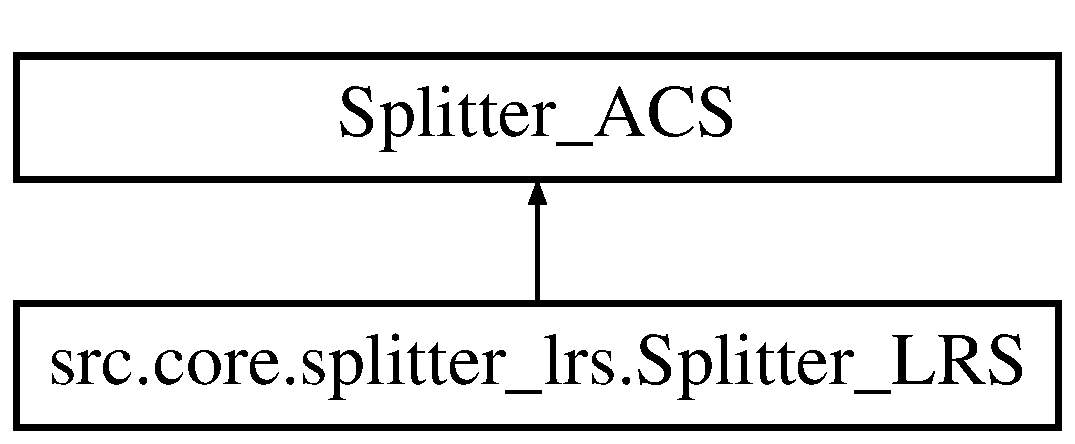
\includegraphics[height=2.000000cm]{classsrc_1_1core_1_1splitter__lrs_1_1Splitter__LRS}
\end{center}
\end{figure}
\subsection*{Public Member Functions}
\begin{DoxyCompactItemize}
\item 
def \hyperlink{classsrc_1_1core_1_1splitter__lrs_1_1Splitter__LRS_a2af1b9374e44f463f69f61070a82b2bf}{\+\_\+\+\_\+init\+\_\+\+\_\+} (self)
\item 
def \hyperlink{classsrc_1_1core_1_1splitter__lrs_1_1Splitter__LRS_a4216d0f000f3484a13199b47a95c25fe}{process\+\_\+lost\+\_\+chunk} (self, lost\+\_\+chunk\+\_\+number, sender)
\item 
def \hyperlink{classsrc_1_1core_1_1splitter__lrs_1_1Splitter__LRS_aaa3ae5c39084168c50d8943a1b37b338}{send\+\_\+chunk} (self, message, peer)
\end{DoxyCompactItemize}
\subsection*{Public Attributes}
\begin{DoxyCompactItemize}
\item 
\hyperlink{classsrc_1_1core_1_1splitter__lrs_1_1Splitter__LRS_aa593047d817d9b5d67b0814fd400d78e}{buffer}
\end{DoxyCompactItemize}


\subsection{Constructor \& Destructor Documentation}
\hypertarget{classsrc_1_1core_1_1splitter__lrs_1_1Splitter__LRS_a2af1b9374e44f463f69f61070a82b2bf}{}\index{src\+::core\+::splitter\+\_\+lrs\+::\+Splitter\+\_\+\+L\+R\+S@{src\+::core\+::splitter\+\_\+lrs\+::\+Splitter\+\_\+\+L\+R\+S}!\+\_\+\+\_\+init\+\_\+\+\_\+@{\+\_\+\+\_\+init\+\_\+\+\_\+}}
\index{\+\_\+\+\_\+init\+\_\+\+\_\+@{\+\_\+\+\_\+init\+\_\+\+\_\+}!src\+::core\+::splitter\+\_\+lrs\+::\+Splitter\+\_\+\+L\+R\+S@{src\+::core\+::splitter\+\_\+lrs\+::\+Splitter\+\_\+\+L\+R\+S}}
\subsubsection[{\+\_\+\+\_\+init\+\_\+\+\_\+}]{\setlength{\rightskip}{0pt plus 5cm}def src.\+core.\+splitter\+\_\+lrs.\+Splitter\+\_\+\+L\+R\+S.\+\_\+\+\_\+init\+\_\+\+\_\+ (
\begin{DoxyParamCaption}
\item[{}]{self}
\end{DoxyParamCaption}
)}\label{classsrc_1_1core_1_1splitter__lrs_1_1Splitter__LRS_a2af1b9374e44f463f69f61070a82b2bf}


\subsection{Member Function Documentation}
\hypertarget{classsrc_1_1core_1_1splitter__lrs_1_1Splitter__LRS_a4216d0f000f3484a13199b47a95c25fe}{}\index{src\+::core\+::splitter\+\_\+lrs\+::\+Splitter\+\_\+\+L\+R\+S@{src\+::core\+::splitter\+\_\+lrs\+::\+Splitter\+\_\+\+L\+R\+S}!process\+\_\+lost\+\_\+chunk@{process\+\_\+lost\+\_\+chunk}}
\index{process\+\_\+lost\+\_\+chunk@{process\+\_\+lost\+\_\+chunk}!src\+::core\+::splitter\+\_\+lrs\+::\+Splitter\+\_\+\+L\+R\+S@{src\+::core\+::splitter\+\_\+lrs\+::\+Splitter\+\_\+\+L\+R\+S}}
\subsubsection[{process\+\_\+lost\+\_\+chunk}]{\setlength{\rightskip}{0pt plus 5cm}def src.\+core.\+splitter\+\_\+lrs.\+Splitter\+\_\+\+L\+R\+S.\+process\+\_\+lost\+\_\+chunk (
\begin{DoxyParamCaption}
\item[{}]{self, }
\item[{}]{lost\+\_\+chunk\+\_\+number, }
\item[{}]{sender}
\end{DoxyParamCaption}
)}\label{classsrc_1_1core_1_1splitter__lrs_1_1Splitter__LRS_a4216d0f000f3484a13199b47a95c25fe}
\hypertarget{classsrc_1_1core_1_1splitter__lrs_1_1Splitter__LRS_aaa3ae5c39084168c50d8943a1b37b338}{}\index{src\+::core\+::splitter\+\_\+lrs\+::\+Splitter\+\_\+\+L\+R\+S@{src\+::core\+::splitter\+\_\+lrs\+::\+Splitter\+\_\+\+L\+R\+S}!send\+\_\+chunk@{send\+\_\+chunk}}
\index{send\+\_\+chunk@{send\+\_\+chunk}!src\+::core\+::splitter\+\_\+lrs\+::\+Splitter\+\_\+\+L\+R\+S@{src\+::core\+::splitter\+\_\+lrs\+::\+Splitter\+\_\+\+L\+R\+S}}
\subsubsection[{send\+\_\+chunk}]{\setlength{\rightskip}{0pt plus 5cm}def src.\+core.\+splitter\+\_\+lrs.\+Splitter\+\_\+\+L\+R\+S.\+send\+\_\+chunk (
\begin{DoxyParamCaption}
\item[{}]{self, }
\item[{}]{message, }
\item[{}]{peer}
\end{DoxyParamCaption}
)}\label{classsrc_1_1core_1_1splitter__lrs_1_1Splitter__LRS_aaa3ae5c39084168c50d8943a1b37b338}


\subsection{Member Data Documentation}
\hypertarget{classsrc_1_1core_1_1splitter__lrs_1_1Splitter__LRS_aa593047d817d9b5d67b0814fd400d78e}{}\index{src\+::core\+::splitter\+\_\+lrs\+::\+Splitter\+\_\+\+L\+R\+S@{src\+::core\+::splitter\+\_\+lrs\+::\+Splitter\+\_\+\+L\+R\+S}!buffer@{buffer}}
\index{buffer@{buffer}!src\+::core\+::splitter\+\_\+lrs\+::\+Splitter\+\_\+\+L\+R\+S@{src\+::core\+::splitter\+\_\+lrs\+::\+Splitter\+\_\+\+L\+R\+S}}
\subsubsection[{buffer}]{\setlength{\rightskip}{0pt plus 5cm}src.\+core.\+splitter\+\_\+lrs.\+Splitter\+\_\+\+L\+R\+S.\+buffer}\label{classsrc_1_1core_1_1splitter__lrs_1_1Splitter__LRS_aa593047d817d9b5d67b0814fd400d78e}


The documentation for this class was generated from the following file\+:\begin{DoxyCompactItemize}
\item 
src/core/\hyperlink{splitter__lrs_8py}{splitter\+\_\+lrs.\+py}\end{DoxyCompactItemize}

\hypertarget{classsrc_1_1lib_1_1vlc_1_1State}{}\section{src.\+lib.\+vlc.\+State Class Reference}
\label{classsrc_1_1lib_1_1vlc_1_1State}\index{src.\+lib.\+vlc.\+State@{src.\+lib.\+vlc.\+State}}
Inheritance diagram for src.\+lib.\+vlc.\+State\+:\begin{figure}[H]
\begin{center}
\leavevmode
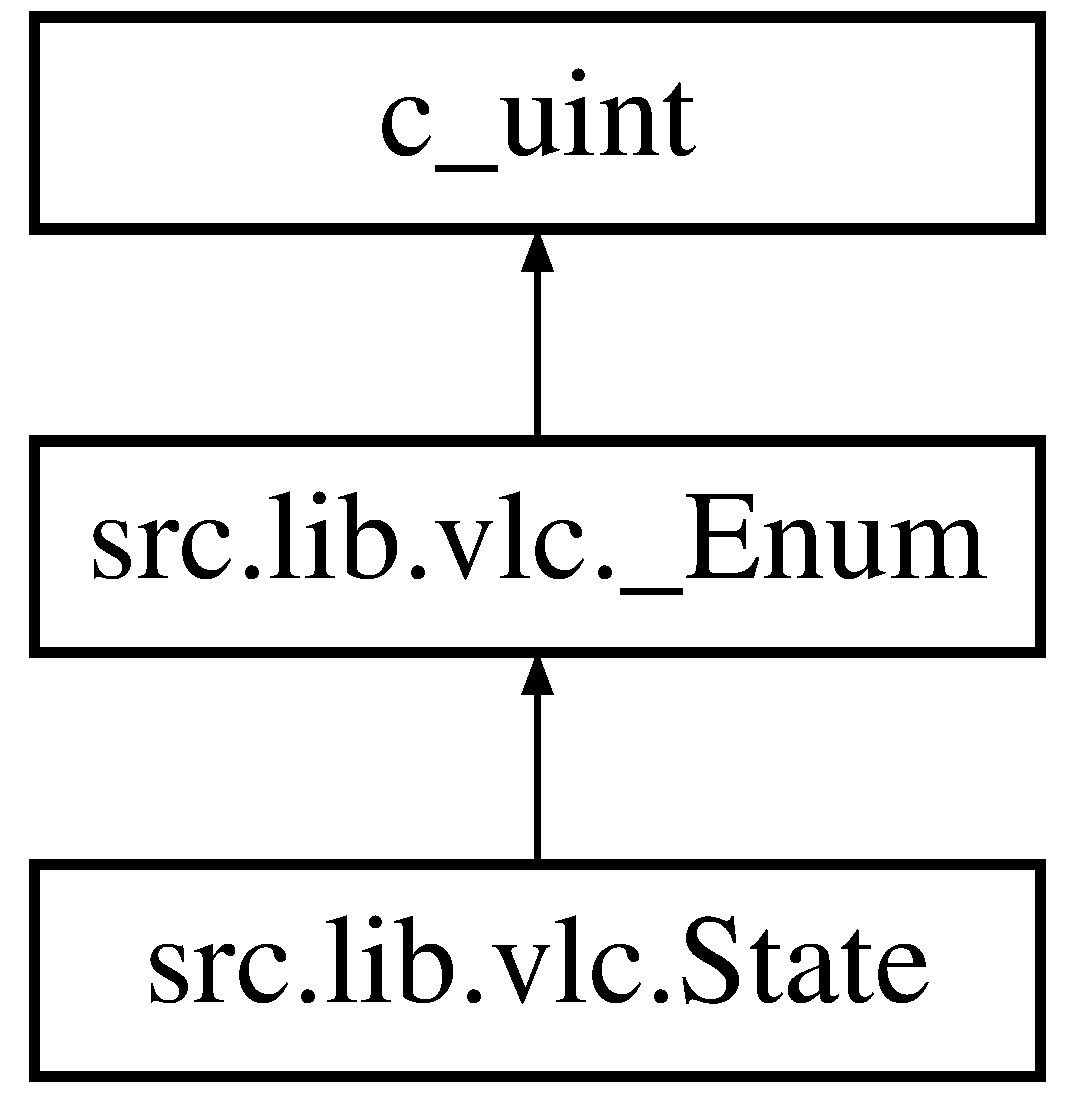
\includegraphics[height=3.000000cm]{classsrc_1_1lib_1_1vlc_1_1State}
\end{center}
\end{figure}
\subsection*{Static Private Attributes}
\begin{DoxyCompactItemize}
\item 
dictionary \hyperlink{classsrc_1_1lib_1_1vlc_1_1State_a3e2fd195ae0b293c4ed0dd8ecc5d229f}{\+\_\+enum\+\_\+names\+\_\+}
\end{DoxyCompactItemize}
\subsection*{Additional Inherited Members}


\subsection{Detailed Description}
\begin{DoxyVerb}Note the order of libvlc_state_t enum must match exactly the order of
See mediacontrol_playerstatus, See input_state_e enums,
and videolan.libvlc.state (at bindings/cil/src/media.cs).
expected states by web plugins are:
idle/close=0, opening=1, buffering=2, playing=3, paused=4,
stopping=5, ended=6, error=7.
\end{DoxyVerb}
 

\subsection{Member Data Documentation}
\hypertarget{classsrc_1_1lib_1_1vlc_1_1State_a3e2fd195ae0b293c4ed0dd8ecc5d229f}{}\index{src\+::lib\+::vlc\+::\+State@{src\+::lib\+::vlc\+::\+State}!\+\_\+enum\+\_\+names\+\_\+@{\+\_\+enum\+\_\+names\+\_\+}}
\index{\+\_\+enum\+\_\+names\+\_\+@{\+\_\+enum\+\_\+names\+\_\+}!src\+::lib\+::vlc\+::\+State@{src\+::lib\+::vlc\+::\+State}}
\subsubsection[{\+\_\+enum\+\_\+names\+\_\+}]{\setlength{\rightskip}{0pt plus 5cm}dictionary src.\+lib.\+vlc.\+State.\+\_\+enum\+\_\+names\+\_\+\hspace{0.3cm}{\ttfamily [static]}, {\ttfamily [private]}}\label{classsrc_1_1lib_1_1vlc_1_1State_a3e2fd195ae0b293c4ed0dd8ecc5d229f}
{\bfseries Initial value\+:}
\begin{DoxyCode}
1 = \{
2         0: \textcolor{stringliteral}{'NothingSpecial'},
3         1: \textcolor{stringliteral}{'Opening'},
4         2: \textcolor{stringliteral}{'Buffering'},
5         3: \textcolor{stringliteral}{'Playing'},
6         4: \textcolor{stringliteral}{'Paused'},
7         5: \textcolor{stringliteral}{'Stopped'},
8         6: \textcolor{stringliteral}{'Ended'},
9         7: \textcolor{stringliteral}{'Error'},
10     \}
\end{DoxyCode}


The documentation for this class was generated from the following file\+:\begin{DoxyCompactItemize}
\item 
src/lib/\hyperlink{vlc_8py}{vlc.\+py}\end{DoxyCompactItemize}

\hypertarget{classsrc_1_1lib_1_1vlc_1_1TrackDescription}{}\section{src.\+lib.\+vlc.\+Track\+Description Class Reference}
\label{classsrc_1_1lib_1_1vlc_1_1TrackDescription}\index{src.\+lib.\+vlc.\+Track\+Description@{src.\+lib.\+vlc.\+Track\+Description}}
Inheritance diagram for src.\+lib.\+vlc.\+Track\+Description\+:\begin{figure}[H]
\begin{center}
\leavevmode
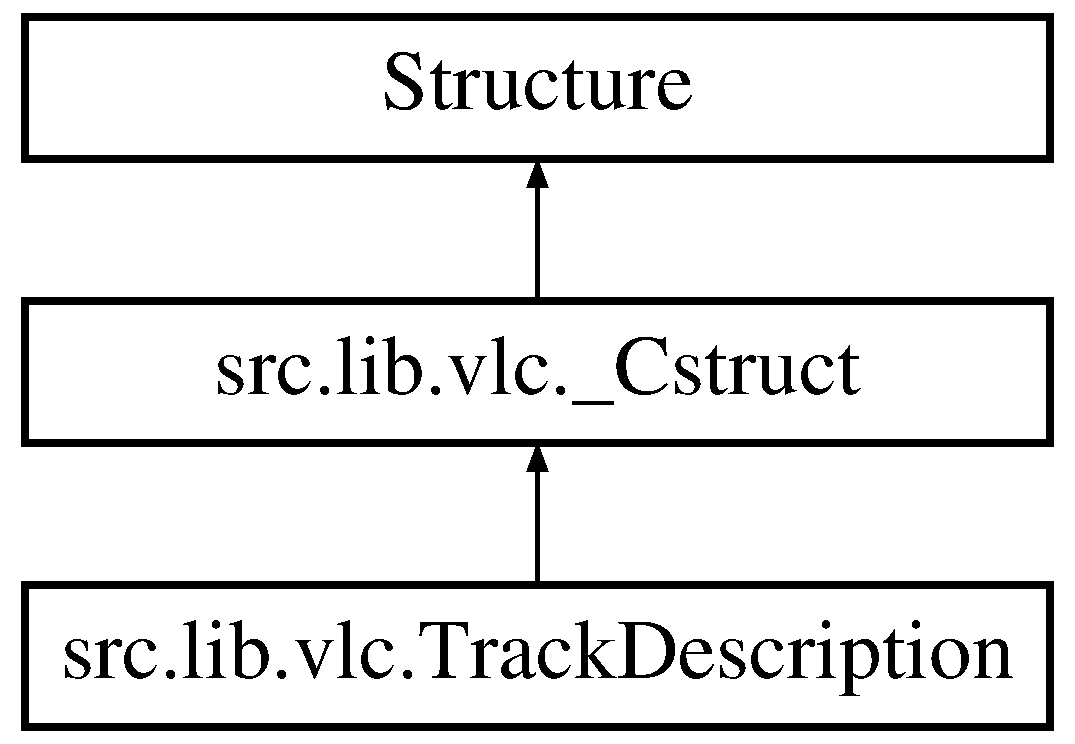
\includegraphics[height=3.000000cm]{classsrc_1_1lib_1_1vlc_1_1TrackDescription}
\end{center}
\end{figure}
\subsection*{Public Member Functions}
\begin{DoxyCompactItemize}
\item 
def \hyperlink{classsrc_1_1lib_1_1vlc_1_1TrackDescription_a2e4ed3042083027afc056bdcb521c6d3}{\+\_\+\+\_\+str\+\_\+\+\_\+} (self)
\end{DoxyCompactItemize}


\subsection{Member Function Documentation}
\hypertarget{classsrc_1_1lib_1_1vlc_1_1TrackDescription_a2e4ed3042083027afc056bdcb521c6d3}{}\index{src\+::lib\+::vlc\+::\+Track\+Description@{src\+::lib\+::vlc\+::\+Track\+Description}!\+\_\+\+\_\+str\+\_\+\+\_\+@{\+\_\+\+\_\+str\+\_\+\+\_\+}}
\index{\+\_\+\+\_\+str\+\_\+\+\_\+@{\+\_\+\+\_\+str\+\_\+\+\_\+}!src\+::lib\+::vlc\+::\+Track\+Description@{src\+::lib\+::vlc\+::\+Track\+Description}}
\subsubsection[{\+\_\+\+\_\+str\+\_\+\+\_\+}]{\setlength{\rightskip}{0pt plus 5cm}def src.\+lib.\+vlc.\+Track\+Description.\+\_\+\+\_\+str\+\_\+\+\_\+ (
\begin{DoxyParamCaption}
\item[{}]{self}
\end{DoxyParamCaption}
)}\label{classsrc_1_1lib_1_1vlc_1_1TrackDescription_a2e4ed3042083027afc056bdcb521c6d3}


The documentation for this class was generated from the following file\+:\begin{DoxyCompactItemize}
\item 
src/lib/\hyperlink{vlc_8py}{vlc.\+py}\end{DoxyCompactItemize}

\hypertarget{classsrc_1_1lib_1_1vlc_1_1TrackType}{}\section{src.\+lib.\+vlc.\+Track\+Type Class Reference}
\label{classsrc_1_1lib_1_1vlc_1_1TrackType}\index{src.\+lib.\+vlc.\+Track\+Type@{src.\+lib.\+vlc.\+Track\+Type}}
Inheritance diagram for src.\+lib.\+vlc.\+Track\+Type\+:\begin{figure}[H]
\begin{center}
\leavevmode
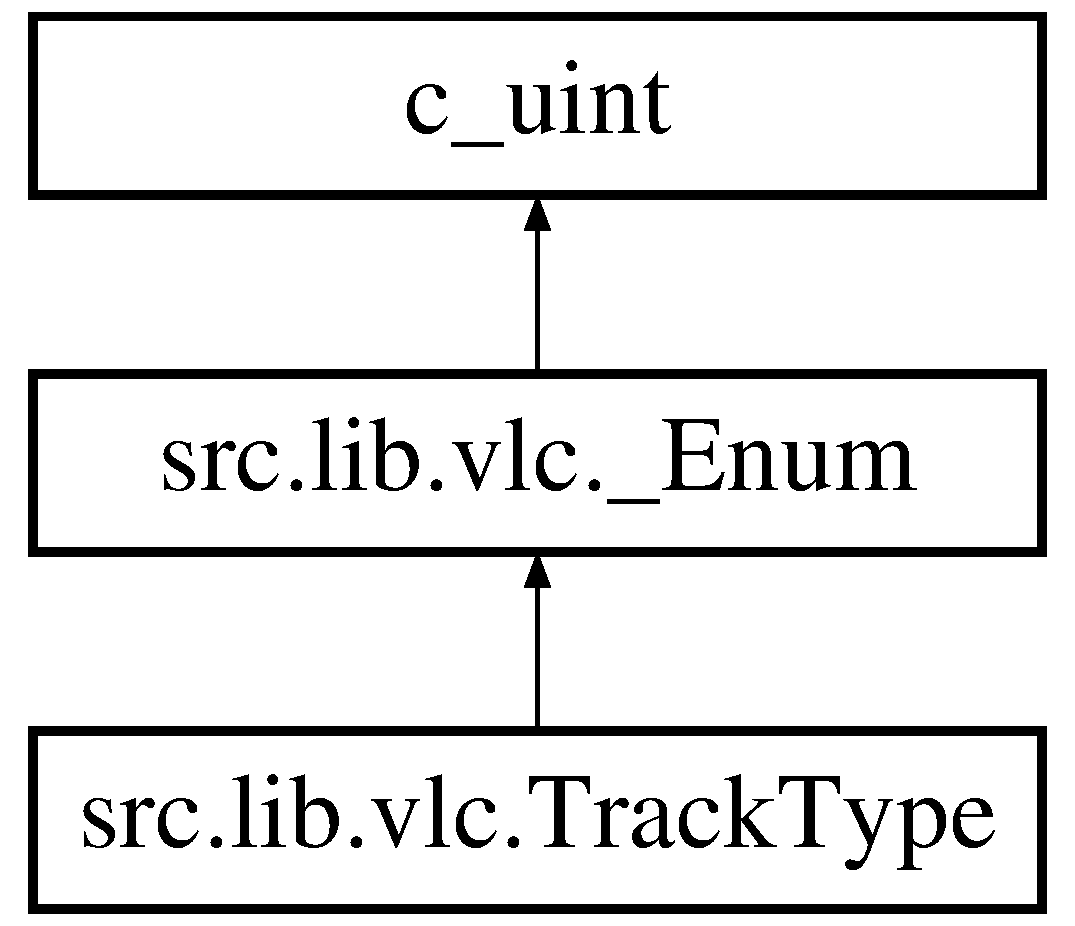
\includegraphics[height=3.000000cm]{classsrc_1_1lib_1_1vlc_1_1TrackType}
\end{center}
\end{figure}
\subsection*{Static Private Attributes}
\begin{DoxyCompactItemize}
\item 
dictionary \hyperlink{classsrc_1_1lib_1_1vlc_1_1TrackType_aa3208a05816c8c0f30e111fae7974667}{\+\_\+enum\+\_\+names\+\_\+}
\end{DoxyCompactItemize}
\subsection*{Additional Inherited Members}


\subsection{Detailed Description}
\begin{DoxyVerb}N/A
\end{DoxyVerb}
 

\subsection{Member Data Documentation}
\hypertarget{classsrc_1_1lib_1_1vlc_1_1TrackType_aa3208a05816c8c0f30e111fae7974667}{}\index{src\+::lib\+::vlc\+::\+Track\+Type@{src\+::lib\+::vlc\+::\+Track\+Type}!\+\_\+enum\+\_\+names\+\_\+@{\+\_\+enum\+\_\+names\+\_\+}}
\index{\+\_\+enum\+\_\+names\+\_\+@{\+\_\+enum\+\_\+names\+\_\+}!src\+::lib\+::vlc\+::\+Track\+Type@{src\+::lib\+::vlc\+::\+Track\+Type}}
\subsubsection[{\+\_\+enum\+\_\+names\+\_\+}]{\setlength{\rightskip}{0pt plus 5cm}dictionary src.\+lib.\+vlc.\+Track\+Type.\+\_\+enum\+\_\+names\+\_\+\hspace{0.3cm}{\ttfamily [static]}, {\ttfamily [private]}}\label{classsrc_1_1lib_1_1vlc_1_1TrackType_aa3208a05816c8c0f30e111fae7974667}
{\bfseries Initial value\+:}
\begin{DoxyCode}
1 = \{
2         -1: \textcolor{stringliteral}{'unknown'},
3         0: \textcolor{stringliteral}{'audio'},
4         1: \textcolor{stringliteral}{'video'},
5         2: \textcolor{stringliteral}{'text'},
6     \}
\end{DoxyCode}


The documentation for this class was generated from the following file\+:\begin{DoxyCompactItemize}
\item 
src/lib/\hyperlink{vlc_8py}{vlc.\+py}\end{DoxyCompactItemize}

\hypertarget{classsrc_1_1lib_1_1vlc_1_1VideoAdjustOption}{}\section{src.\+lib.\+vlc.\+Video\+Adjust\+Option Class Reference}
\label{classsrc_1_1lib_1_1vlc_1_1VideoAdjustOption}\index{src.\+lib.\+vlc.\+Video\+Adjust\+Option@{src.\+lib.\+vlc.\+Video\+Adjust\+Option}}
Inheritance diagram for src.\+lib.\+vlc.\+Video\+Adjust\+Option\+:\begin{figure}[H]
\begin{center}
\leavevmode
\includegraphics[height=3.000000cm]{classsrc_1_1lib_1_1vlc_1_1VideoAdjustOption}
\end{center}
\end{figure}
\subsection*{Static Private Attributes}
\begin{DoxyCompactItemize}
\item 
dictionary \hyperlink{classsrc_1_1lib_1_1vlc_1_1VideoAdjustOption_aac7ce12bf5da69f9fc78c55cbeea76f4}{\+\_\+enum\+\_\+names\+\_\+}
\end{DoxyCompactItemize}
\subsection*{Additional Inherited Members}


\subsection{Detailed Description}
\begin{DoxyVerb}Option values for libvlc_video_{get,set}_adjust_{int,float,bool}.
\end{DoxyVerb}
 

\subsection{Member Data Documentation}
\hypertarget{classsrc_1_1lib_1_1vlc_1_1VideoAdjustOption_aac7ce12bf5da69f9fc78c55cbeea76f4}{}\index{src\+::lib\+::vlc\+::\+Video\+Adjust\+Option@{src\+::lib\+::vlc\+::\+Video\+Adjust\+Option}!\+\_\+enum\+\_\+names\+\_\+@{\+\_\+enum\+\_\+names\+\_\+}}
\index{\+\_\+enum\+\_\+names\+\_\+@{\+\_\+enum\+\_\+names\+\_\+}!src\+::lib\+::vlc\+::\+Video\+Adjust\+Option@{src\+::lib\+::vlc\+::\+Video\+Adjust\+Option}}
\subsubsection[{\+\_\+enum\+\_\+names\+\_\+}]{\setlength{\rightskip}{0pt plus 5cm}dictionary src.\+lib.\+vlc.\+Video\+Adjust\+Option.\+\_\+enum\+\_\+names\+\_\+\hspace{0.3cm}{\ttfamily [static]}, {\ttfamily [private]}}\label{classsrc_1_1lib_1_1vlc_1_1VideoAdjustOption_aac7ce12bf5da69f9fc78c55cbeea76f4}
{\bfseries Initial value\+:}
\begin{DoxyCode}
1 = \{
2         0: \textcolor{stringliteral}{'Enable'},
3         1: \textcolor{stringliteral}{'Contrast'},
4         2: \textcolor{stringliteral}{'Brightness'},
5         3: \textcolor{stringliteral}{'Hue'},
6         4: \textcolor{stringliteral}{'Saturation'},
7         5: \textcolor{stringliteral}{'Gamma'},
8     \}
\end{DoxyCode}


The documentation for this class was generated from the following file\+:\begin{DoxyCompactItemize}
\item 
src/lib/\hyperlink{vlc_8py}{vlc.\+py}\end{DoxyCompactItemize}

\hypertarget{classsrc_1_1lib_1_1vlc_1_1VideoLogoOption}{}\section{src.\+lib.\+vlc.\+Video\+Logo\+Option Class Reference}
\label{classsrc_1_1lib_1_1vlc_1_1VideoLogoOption}\index{src.\+lib.\+vlc.\+Video\+Logo\+Option@{src.\+lib.\+vlc.\+Video\+Logo\+Option}}
Inheritance diagram for src.\+lib.\+vlc.\+Video\+Logo\+Option\+:\begin{figure}[H]
\begin{center}
\leavevmode
\includegraphics[height=3.000000cm]{classsrc_1_1lib_1_1vlc_1_1VideoLogoOption}
\end{center}
\end{figure}
\subsection*{Static Private Attributes}
\begin{DoxyCompactItemize}
\item 
dictionary \hyperlink{classsrc_1_1lib_1_1vlc_1_1VideoLogoOption_ac64c121a5e6196560c51e4ae1e6b0c77}{\+\_\+enum\+\_\+names\+\_\+}
\end{DoxyCompactItemize}
\subsection*{Additional Inherited Members}


\subsection{Detailed Description}
\begin{DoxyVerb}Option values for libvlc_video_{get,set}_logo_{int,string}.
\end{DoxyVerb}
 

\subsection{Member Data Documentation}
\hypertarget{classsrc_1_1lib_1_1vlc_1_1VideoLogoOption_ac64c121a5e6196560c51e4ae1e6b0c77}{}\index{src\+::lib\+::vlc\+::\+Video\+Logo\+Option@{src\+::lib\+::vlc\+::\+Video\+Logo\+Option}!\+\_\+enum\+\_\+names\+\_\+@{\+\_\+enum\+\_\+names\+\_\+}}
\index{\+\_\+enum\+\_\+names\+\_\+@{\+\_\+enum\+\_\+names\+\_\+}!src\+::lib\+::vlc\+::\+Video\+Logo\+Option@{src\+::lib\+::vlc\+::\+Video\+Logo\+Option}}
\subsubsection[{\+\_\+enum\+\_\+names\+\_\+}]{\setlength{\rightskip}{0pt plus 5cm}dictionary src.\+lib.\+vlc.\+Video\+Logo\+Option.\+\_\+enum\+\_\+names\+\_\+\hspace{0.3cm}{\ttfamily [static]}, {\ttfamily [private]}}\label{classsrc_1_1lib_1_1vlc_1_1VideoLogoOption_ac64c121a5e6196560c51e4ae1e6b0c77}
{\bfseries Initial value\+:}
\begin{DoxyCode}
1 = \{
2         0: \textcolor{stringliteral}{'enable'},
3         1: \textcolor{stringliteral}{'file'},
4         2: \textcolor{stringliteral}{'logo\_x'},
5         3: \textcolor{stringliteral}{'logo\_y'},
6         4: \textcolor{stringliteral}{'delay'},
7         5: \textcolor{stringliteral}{'repeat'},
8         6: \textcolor{stringliteral}{'opacity'},
9         7: \textcolor{stringliteral}{'position'},
10     \}
\end{DoxyCode}


The documentation for this class was generated from the following file\+:\begin{DoxyCompactItemize}
\item 
src/lib/\hyperlink{vlc_8py}{vlc.\+py}\end{DoxyCompactItemize}

\hypertarget{classsrc_1_1lib_1_1vlc_1_1VideoMarqueeOption}{}\section{src.\+lib.\+vlc.\+Video\+Marquee\+Option Class Reference}
\label{classsrc_1_1lib_1_1vlc_1_1VideoMarqueeOption}\index{src.\+lib.\+vlc.\+Video\+Marquee\+Option@{src.\+lib.\+vlc.\+Video\+Marquee\+Option}}
Inheritance diagram for src.\+lib.\+vlc.\+Video\+Marquee\+Option\+:\begin{figure}[H]
\begin{center}
\leavevmode
\includegraphics[height=3.000000cm]{classsrc_1_1lib_1_1vlc_1_1VideoMarqueeOption}
\end{center}
\end{figure}
\subsection*{Static Private Attributes}
\begin{DoxyCompactItemize}
\item 
dictionary \hyperlink{classsrc_1_1lib_1_1vlc_1_1VideoMarqueeOption_a211a7ad22269a5ebbdd3a7883077ff3e}{\+\_\+enum\+\_\+names\+\_\+}
\end{DoxyCompactItemize}
\subsection*{Additional Inherited Members}


\subsection{Detailed Description}
\begin{DoxyVerb}Marq options definition.
\end{DoxyVerb}
 

\subsection{Member Data Documentation}
\hypertarget{classsrc_1_1lib_1_1vlc_1_1VideoMarqueeOption_a211a7ad22269a5ebbdd3a7883077ff3e}{}\index{src\+::lib\+::vlc\+::\+Video\+Marquee\+Option@{src\+::lib\+::vlc\+::\+Video\+Marquee\+Option}!\+\_\+enum\+\_\+names\+\_\+@{\+\_\+enum\+\_\+names\+\_\+}}
\index{\+\_\+enum\+\_\+names\+\_\+@{\+\_\+enum\+\_\+names\+\_\+}!src\+::lib\+::vlc\+::\+Video\+Marquee\+Option@{src\+::lib\+::vlc\+::\+Video\+Marquee\+Option}}
\subsubsection[{\+\_\+enum\+\_\+names\+\_\+}]{\setlength{\rightskip}{0pt plus 5cm}dictionary src.\+lib.\+vlc.\+Video\+Marquee\+Option.\+\_\+enum\+\_\+names\+\_\+\hspace{0.3cm}{\ttfamily [static]}, {\ttfamily [private]}}\label{classsrc_1_1lib_1_1vlc_1_1VideoMarqueeOption_a211a7ad22269a5ebbdd3a7883077ff3e}
{\bfseries Initial value\+:}
\begin{DoxyCode}
1 = \{
2         0: \textcolor{stringliteral}{'Enable'},
3         1: \textcolor{stringliteral}{'Text'},
4         2: \textcolor{stringliteral}{'Color'},
5         3: \textcolor{stringliteral}{'Opacity'},
6         4: \textcolor{stringliteral}{'Position'},
7         5: \textcolor{stringliteral}{'Refresh'},
8         6: \textcolor{stringliteral}{'Size'},
9         7: \textcolor{stringliteral}{'Timeout'},
10         8: \textcolor{stringliteral}{'marquee\_X'},
11         9: \textcolor{stringliteral}{'marquee\_Y'},
12     \}
\end{DoxyCode}


The documentation for this class was generated from the following file\+:\begin{DoxyCompactItemize}
\item 
src/lib/\hyperlink{vlc_8py}{vlc.\+py}\end{DoxyCompactItemize}

\hypertarget{classsrc_1_1model_1_1vlc__player_1_1VLC__Player}{}\section{src.\+model.\+vlc\+\_\+player.\+V\+L\+C\+\_\+\+Player Class Reference}
\label{classsrc_1_1model_1_1vlc__player_1_1VLC__Player}\index{src.\+model.\+vlc\+\_\+player.\+V\+L\+C\+\_\+\+Player@{src.\+model.\+vlc\+\_\+player.\+V\+L\+C\+\_\+\+Player}}
\subsection*{Public Member Functions}
\begin{DoxyCompactItemize}
\item 
def \hyperlink{classsrc_1_1model_1_1vlc__player_1_1VLC__Player_ab09b2cb2fbf9f42eb230b76f9d4d2118}{\+\_\+\+\_\+init\+\_\+\+\_\+} (self)
\item 
def \hyperlink{classsrc_1_1model_1_1vlc__player_1_1VLC__Player_a27a50c4399258098ac47e2e2b5d7521e}{media\+\_\+player} (self, win\+\_\+id, Source)
\item 
def \hyperlink{classsrc_1_1model_1_1vlc__player_1_1VLC__Player_a91bfb17633c591cdb9311af985fa8366}{stream\+\_\+player} (self, win\+\_\+id, mrl)
\end{DoxyCompactItemize}
\subsection*{Public Attributes}
\begin{DoxyCompactItemize}
\item 
\hyperlink{classsrc_1_1model_1_1vlc__player_1_1VLC__Player_a1a219abbd53bd508fcc8784ff300a3bd}{vlc\+Instance}
\item 
\hyperlink{classsrc_1_1model_1_1vlc__player_1_1VLC__Player_a589585abc542dbde1e3c3a9d94384875}{player}
\end{DoxyCompactItemize}
\subsection*{Static Public Attributes}
\begin{DoxyCompactItemize}
\item 
string \hyperlink{classsrc_1_1model_1_1vlc__player_1_1VLC__Player_ae218983da86ed762827885423785dab6}{M\+E\+D\+I\+A\+\_\+\+S\+O\+U\+R\+C\+E} = \char`\"{}\char`\"{}
\end{DoxyCompactItemize}
\subsection*{Private Member Functions}
\begin{DoxyCompactItemize}
\item 
def \hyperlink{classsrc_1_1model_1_1vlc__player_1_1VLC__Player_a10170928ceb9974f80d362062d2b1951}{\+\_\+get\+\_\+media} (self, Source)
\item 
def \hyperlink{classsrc_1_1model_1_1vlc__player_1_1VLC__Player_adf11f7e751a9f853ae4f4606baa85693}{\+\_\+set\+\_\+win\+\_\+id} (self, win\+\_\+id)
\item 
def \hyperlink{classsrc_1_1model_1_1vlc__player_1_1VLC__Player_aa4256e7b298fe7b26d60ad7c81a0585d}{\+\_\+set\+\_\+mrl} (self, mrl)
\item 
def \hyperlink{classsrc_1_1model_1_1vlc__player_1_1VLC__Player_a88b754af0a2de61405b8a21ace49c4f1}{\+\_\+set\+\_\+media} (self, Source)
\end{DoxyCompactItemize}


\subsection{Detailed Description}
\begin{DoxyVerb}classdocs
\end{DoxyVerb}
 

\subsection{Constructor \& Destructor Documentation}
\hypertarget{classsrc_1_1model_1_1vlc__player_1_1VLC__Player_ab09b2cb2fbf9f42eb230b76f9d4d2118}{}\index{src\+::model\+::vlc\+\_\+player\+::\+V\+L\+C\+\_\+\+Player@{src\+::model\+::vlc\+\_\+player\+::\+V\+L\+C\+\_\+\+Player}!\+\_\+\+\_\+init\+\_\+\+\_\+@{\+\_\+\+\_\+init\+\_\+\+\_\+}}
\index{\+\_\+\+\_\+init\+\_\+\+\_\+@{\+\_\+\+\_\+init\+\_\+\+\_\+}!src\+::model\+::vlc\+\_\+player\+::\+V\+L\+C\+\_\+\+Player@{src\+::model\+::vlc\+\_\+player\+::\+V\+L\+C\+\_\+\+Player}}
\subsubsection[{\+\_\+\+\_\+init\+\_\+\+\_\+}]{\setlength{\rightskip}{0pt plus 5cm}def src.\+model.\+vlc\+\_\+player.\+V\+L\+C\+\_\+\+Player.\+\_\+\+\_\+init\+\_\+\+\_\+ (
\begin{DoxyParamCaption}
\item[{}]{self}
\end{DoxyParamCaption}
)}\label{classsrc_1_1model_1_1vlc__player_1_1VLC__Player_ab09b2cb2fbf9f42eb230b76f9d4d2118}
\begin{DoxyVerb}Constructor
\end{DoxyVerb}
 

\subsection{Member Function Documentation}
\hypertarget{classsrc_1_1model_1_1vlc__player_1_1VLC__Player_a10170928ceb9974f80d362062d2b1951}{}\index{src\+::model\+::vlc\+\_\+player\+::\+V\+L\+C\+\_\+\+Player@{src\+::model\+::vlc\+\_\+player\+::\+V\+L\+C\+\_\+\+Player}!\+\_\+get\+\_\+media@{\+\_\+get\+\_\+media}}
\index{\+\_\+get\+\_\+media@{\+\_\+get\+\_\+media}!src\+::model\+::vlc\+\_\+player\+::\+V\+L\+C\+\_\+\+Player@{src\+::model\+::vlc\+\_\+player\+::\+V\+L\+C\+\_\+\+Player}}
\subsubsection[{\+\_\+get\+\_\+media}]{\setlength{\rightskip}{0pt plus 5cm}def src.\+model.\+vlc\+\_\+player.\+V\+L\+C\+\_\+\+Player.\+\_\+get\+\_\+media (
\begin{DoxyParamCaption}
\item[{}]{self, }
\item[{}]{Source}
\end{DoxyParamCaption}
)\hspace{0.3cm}{\ttfamily [private]}}\label{classsrc_1_1model_1_1vlc__player_1_1VLC__Player_a10170928ceb9974f80d362062d2b1951}
\hypertarget{classsrc_1_1model_1_1vlc__player_1_1VLC__Player_a88b754af0a2de61405b8a21ace49c4f1}{}\index{src\+::model\+::vlc\+\_\+player\+::\+V\+L\+C\+\_\+\+Player@{src\+::model\+::vlc\+\_\+player\+::\+V\+L\+C\+\_\+\+Player}!\+\_\+set\+\_\+media@{\+\_\+set\+\_\+media}}
\index{\+\_\+set\+\_\+media@{\+\_\+set\+\_\+media}!src\+::model\+::vlc\+\_\+player\+::\+V\+L\+C\+\_\+\+Player@{src\+::model\+::vlc\+\_\+player\+::\+V\+L\+C\+\_\+\+Player}}
\subsubsection[{\+\_\+set\+\_\+media}]{\setlength{\rightskip}{0pt plus 5cm}def src.\+model.\+vlc\+\_\+player.\+V\+L\+C\+\_\+\+Player.\+\_\+set\+\_\+media (
\begin{DoxyParamCaption}
\item[{}]{self, }
\item[{}]{Source}
\end{DoxyParamCaption}
)\hspace{0.3cm}{\ttfamily [private]}}\label{classsrc_1_1model_1_1vlc__player_1_1VLC__Player_a88b754af0a2de61405b8a21ace49c4f1}
\hypertarget{classsrc_1_1model_1_1vlc__player_1_1VLC__Player_aa4256e7b298fe7b26d60ad7c81a0585d}{}\index{src\+::model\+::vlc\+\_\+player\+::\+V\+L\+C\+\_\+\+Player@{src\+::model\+::vlc\+\_\+player\+::\+V\+L\+C\+\_\+\+Player}!\+\_\+set\+\_\+mrl@{\+\_\+set\+\_\+mrl}}
\index{\+\_\+set\+\_\+mrl@{\+\_\+set\+\_\+mrl}!src\+::model\+::vlc\+\_\+player\+::\+V\+L\+C\+\_\+\+Player@{src\+::model\+::vlc\+\_\+player\+::\+V\+L\+C\+\_\+\+Player}}
\subsubsection[{\+\_\+set\+\_\+mrl}]{\setlength{\rightskip}{0pt plus 5cm}def src.\+model.\+vlc\+\_\+player.\+V\+L\+C\+\_\+\+Player.\+\_\+set\+\_\+mrl (
\begin{DoxyParamCaption}
\item[{}]{self, }
\item[{}]{mrl}
\end{DoxyParamCaption}
)\hspace{0.3cm}{\ttfamily [private]}}\label{classsrc_1_1model_1_1vlc__player_1_1VLC__Player_aa4256e7b298fe7b26d60ad7c81a0585d}
\hypertarget{classsrc_1_1model_1_1vlc__player_1_1VLC__Player_adf11f7e751a9f853ae4f4606baa85693}{}\index{src\+::model\+::vlc\+\_\+player\+::\+V\+L\+C\+\_\+\+Player@{src\+::model\+::vlc\+\_\+player\+::\+V\+L\+C\+\_\+\+Player}!\+\_\+set\+\_\+win\+\_\+id@{\+\_\+set\+\_\+win\+\_\+id}}
\index{\+\_\+set\+\_\+win\+\_\+id@{\+\_\+set\+\_\+win\+\_\+id}!src\+::model\+::vlc\+\_\+player\+::\+V\+L\+C\+\_\+\+Player@{src\+::model\+::vlc\+\_\+player\+::\+V\+L\+C\+\_\+\+Player}}
\subsubsection[{\+\_\+set\+\_\+win\+\_\+id}]{\setlength{\rightskip}{0pt plus 5cm}def src.\+model.\+vlc\+\_\+player.\+V\+L\+C\+\_\+\+Player.\+\_\+set\+\_\+win\+\_\+id (
\begin{DoxyParamCaption}
\item[{}]{self, }
\item[{}]{win\+\_\+id}
\end{DoxyParamCaption}
)\hspace{0.3cm}{\ttfamily [private]}}\label{classsrc_1_1model_1_1vlc__player_1_1VLC__Player_adf11f7e751a9f853ae4f4606baa85693}
\hypertarget{classsrc_1_1model_1_1vlc__player_1_1VLC__Player_a27a50c4399258098ac47e2e2b5d7521e}{}\index{src\+::model\+::vlc\+\_\+player\+::\+V\+L\+C\+\_\+\+Player@{src\+::model\+::vlc\+\_\+player\+::\+V\+L\+C\+\_\+\+Player}!media\+\_\+player@{media\+\_\+player}}
\index{media\+\_\+player@{media\+\_\+player}!src\+::model\+::vlc\+\_\+player\+::\+V\+L\+C\+\_\+\+Player@{src\+::model\+::vlc\+\_\+player\+::\+V\+L\+C\+\_\+\+Player}}
\subsubsection[{media\+\_\+player}]{\setlength{\rightskip}{0pt plus 5cm}def src.\+model.\+vlc\+\_\+player.\+V\+L\+C\+\_\+\+Player.\+media\+\_\+player (
\begin{DoxyParamCaption}
\item[{}]{self, }
\item[{}]{win\+\_\+id, }
\item[{}]{Source}
\end{DoxyParamCaption}
)}\label{classsrc_1_1model_1_1vlc__player_1_1VLC__Player_a27a50c4399258098ac47e2e2b5d7521e}
\hypertarget{classsrc_1_1model_1_1vlc__player_1_1VLC__Player_a91bfb17633c591cdb9311af985fa8366}{}\index{src\+::model\+::vlc\+\_\+player\+::\+V\+L\+C\+\_\+\+Player@{src\+::model\+::vlc\+\_\+player\+::\+V\+L\+C\+\_\+\+Player}!stream\+\_\+player@{stream\+\_\+player}}
\index{stream\+\_\+player@{stream\+\_\+player}!src\+::model\+::vlc\+\_\+player\+::\+V\+L\+C\+\_\+\+Player@{src\+::model\+::vlc\+\_\+player\+::\+V\+L\+C\+\_\+\+Player}}
\subsubsection[{stream\+\_\+player}]{\setlength{\rightskip}{0pt plus 5cm}def src.\+model.\+vlc\+\_\+player.\+V\+L\+C\+\_\+\+Player.\+stream\+\_\+player (
\begin{DoxyParamCaption}
\item[{}]{self, }
\item[{}]{win\+\_\+id, }
\item[{}]{mrl}
\end{DoxyParamCaption}
)}\label{classsrc_1_1model_1_1vlc__player_1_1VLC__Player_a91bfb17633c591cdb9311af985fa8366}


\subsection{Member Data Documentation}
\hypertarget{classsrc_1_1model_1_1vlc__player_1_1VLC__Player_ae218983da86ed762827885423785dab6}{}\index{src\+::model\+::vlc\+\_\+player\+::\+V\+L\+C\+\_\+\+Player@{src\+::model\+::vlc\+\_\+player\+::\+V\+L\+C\+\_\+\+Player}!M\+E\+D\+I\+A\+\_\+\+S\+O\+U\+R\+C\+E@{M\+E\+D\+I\+A\+\_\+\+S\+O\+U\+R\+C\+E}}
\index{M\+E\+D\+I\+A\+\_\+\+S\+O\+U\+R\+C\+E@{M\+E\+D\+I\+A\+\_\+\+S\+O\+U\+R\+C\+E}!src\+::model\+::vlc\+\_\+player\+::\+V\+L\+C\+\_\+\+Player@{src\+::model\+::vlc\+\_\+player\+::\+V\+L\+C\+\_\+\+Player}}
\subsubsection[{M\+E\+D\+I\+A\+\_\+\+S\+O\+U\+R\+C\+E}]{\setlength{\rightskip}{0pt plus 5cm}string src.\+model.\+vlc\+\_\+player.\+V\+L\+C\+\_\+\+Player.\+M\+E\+D\+I\+A\+\_\+\+S\+O\+U\+R\+C\+E = \char`\"{}\char`\"{}\hspace{0.3cm}{\ttfamily [static]}}\label{classsrc_1_1model_1_1vlc__player_1_1VLC__Player_ae218983da86ed762827885423785dab6}
\hypertarget{classsrc_1_1model_1_1vlc__player_1_1VLC__Player_a589585abc542dbde1e3c3a9d94384875}{}\index{src\+::model\+::vlc\+\_\+player\+::\+V\+L\+C\+\_\+\+Player@{src\+::model\+::vlc\+\_\+player\+::\+V\+L\+C\+\_\+\+Player}!player@{player}}
\index{player@{player}!src\+::model\+::vlc\+\_\+player\+::\+V\+L\+C\+\_\+\+Player@{src\+::model\+::vlc\+\_\+player\+::\+V\+L\+C\+\_\+\+Player}}
\subsubsection[{player}]{\setlength{\rightskip}{0pt plus 5cm}src.\+model.\+vlc\+\_\+player.\+V\+L\+C\+\_\+\+Player.\+player}\label{classsrc_1_1model_1_1vlc__player_1_1VLC__Player_a589585abc542dbde1e3c3a9d94384875}
\hypertarget{classsrc_1_1model_1_1vlc__player_1_1VLC__Player_a1a219abbd53bd508fcc8784ff300a3bd}{}\index{src\+::model\+::vlc\+\_\+player\+::\+V\+L\+C\+\_\+\+Player@{src\+::model\+::vlc\+\_\+player\+::\+V\+L\+C\+\_\+\+Player}!vlc\+Instance@{vlc\+Instance}}
\index{vlc\+Instance@{vlc\+Instance}!src\+::model\+::vlc\+\_\+player\+::\+V\+L\+C\+\_\+\+Player@{src\+::model\+::vlc\+\_\+player\+::\+V\+L\+C\+\_\+\+Player}}
\subsubsection[{vlc\+Instance}]{\setlength{\rightskip}{0pt plus 5cm}src.\+model.\+vlc\+\_\+player.\+V\+L\+C\+\_\+\+Player.\+vlc\+Instance}\label{classsrc_1_1model_1_1vlc__player_1_1VLC__Player_a1a219abbd53bd508fcc8784ff300a3bd}


The documentation for this class was generated from the following file\+:\begin{DoxyCompactItemize}
\item 
src/model/\hyperlink{vlc__player_8py}{vlc\+\_\+player.\+py}\end{DoxyCompactItemize}

\hypertarget{classsrc_1_1lib_1_1vlc_1_1VLCException}{}\section{src.\+lib.\+vlc.\+V\+L\+C\+Exception Class Reference}
\label{classsrc_1_1lib_1_1vlc_1_1VLCException}\index{src.\+lib.\+vlc.\+V\+L\+C\+Exception@{src.\+lib.\+vlc.\+V\+L\+C\+Exception}}
Inheritance diagram for src.\+lib.\+vlc.\+V\+L\+C\+Exception\+:\begin{figure}[H]
\begin{center}
\leavevmode
\includegraphics[height=2.000000cm]{classsrc_1_1lib_1_1vlc_1_1VLCException}
\end{center}
\end{figure}


\subsection{Detailed Description}
\begin{DoxyVerb}Exception raised by libvlc methods.
\end{DoxyVerb}
 

The documentation for this class was generated from the following file\+:\begin{DoxyCompactItemize}
\item 
src/lib/\hyperlink{vlc_8py}{vlc.\+py}\end{DoxyCompactItemize}

\chapter{File Documentation}
\hypertarget{P2PSP_8md}{}\section{doc/\+P2\+P\+S\+P.md File Reference}
\label{P2PSP_8md}\index{doc/\+P2\+P\+S\+P.\+md@{doc/\+P2\+P\+S\+P.\+md}}

\hypertarget{VirtualBox_8md}{}\section{doc/\+Virtual\+Box.md File Reference}
\label{VirtualBox_8md}\index{doc/\+Virtual\+Box.\+md@{doc/\+Virtual\+Box.\+md}}

\hypertarget{VLC_8md}{}\section{doc/\+V\+L\+C.md File Reference}
\label{VLC_8md}\index{doc/\+V\+L\+C.\+md@{doc/\+V\+L\+C.\+md}}

\hypertarget{windows_8md}{}\section{doc/windows.md File Reference}
\label{windows_8md}\index{doc/windows.\+md@{doc/windows.\+md}}

\hypertarget{README_8md}{}\section{R\+E\+A\+D\+M\+E.\+md File Reference}
\label{README_8md}\index{R\+E\+A\+D\+M\+E.\+md@{R\+E\+A\+D\+M\+E.\+md}}

\hypertarget{____init_____8py}{}\section{src/\+\_\+\+\_\+init\+\_\+\+\_\+.py File Reference}
\label{____init_____8py}\index{src/\+\_\+\+\_\+init\+\_\+\+\_\+.\+py@{src/\+\_\+\+\_\+init\+\_\+\+\_\+.\+py}}
\subsection*{Namespaces}
\begin{DoxyCompactItemize}
\item 
 \hyperlink{namespacesrc}{src}
\end{DoxyCompactItemize}

\hypertarget{adapter_2____init_____8py}{}\section{src/adapter/\+\_\+\+\_\+init\+\_\+\+\_\+.py File Reference}
\label{adapter_2____init_____8py}\index{src/adapter/\+\_\+\+\_\+init\+\_\+\+\_\+.\+py@{src/adapter/\+\_\+\+\_\+init\+\_\+\+\_\+.\+py}}
\subsection*{Namespaces}
\begin{DoxyCompactItemize}
\item 
 \hyperlink{namespacesrc_1_1adapter}{src.\+adapter}
\end{DoxyCompactItemize}

\hypertarget{common_2____init_____8py}{}\section{src/common/\+\_\+\+\_\+init\+\_\+\+\_\+.py File Reference}
\label{common_2____init_____8py}\index{src/common/\+\_\+\+\_\+init\+\_\+\+\_\+.\+py@{src/common/\+\_\+\+\_\+init\+\_\+\+\_\+.\+py}}
\subsection*{Namespaces}
\begin{DoxyCompactItemize}
\item 
 \hyperlink{namespacesrc_1_1common}{src.\+common}
\end{DoxyCompactItemize}

\hypertarget{controller_2____init_____8py}{}\section{src/controller/\+\_\+\+\_\+init\+\_\+\+\_\+.py File Reference}
\label{controller_2____init_____8py}\index{src/controller/\+\_\+\+\_\+init\+\_\+\+\_\+.\+py@{src/controller/\+\_\+\+\_\+init\+\_\+\+\_\+.\+py}}
\subsection*{Namespaces}
\begin{DoxyCompactItemize}
\item 
 \hyperlink{namespacesrc_1_1controller}{src.\+controller}
\end{DoxyCompactItemize}

\hypertarget{core_2____init_____8py}{}\section{src/core/\+\_\+\+\_\+init\+\_\+\+\_\+.py File Reference}
\label{core_2____init_____8py}\index{src/core/\+\_\+\+\_\+init\+\_\+\+\_\+.\+py@{src/core/\+\_\+\+\_\+init\+\_\+\+\_\+.\+py}}
\subsection*{Namespaces}
\begin{DoxyCompactItemize}
\item 
 \hyperlink{namespacesrc_1_1core}{src.\+core}
\end{DoxyCompactItemize}

\hypertarget{lib_2____init_____8py}{}\section{src/lib/\+\_\+\+\_\+init\+\_\+\+\_\+.py File Reference}
\label{lib_2____init_____8py}\index{src/lib/\+\_\+\+\_\+init\+\_\+\+\_\+.\+py@{src/lib/\+\_\+\+\_\+init\+\_\+\+\_\+.\+py}}
\subsection*{Namespaces}
\begin{DoxyCompactItemize}
\item 
 \hyperlink{namespacesrc_1_1lib}{src.\+lib}
\end{DoxyCompactItemize}

\hypertarget{model_2____init_____8py}{}\section{src/model/\+\_\+\+\_\+init\+\_\+\+\_\+.py File Reference}
\label{model_2____init_____8py}\index{src/model/\+\_\+\+\_\+init\+\_\+\+\_\+.\+py@{src/model/\+\_\+\+\_\+init\+\_\+\+\_\+.\+py}}
\subsection*{Namespaces}
\begin{DoxyCompactItemize}
\item 
 \hyperlink{namespacesrc_1_1model}{src.\+model}
\end{DoxyCompactItemize}

\hypertarget{view_2____init_____8py}{}\section{src/view/\+\_\+\+\_\+init\+\_\+\+\_\+.py File Reference}
\label{view_2____init_____8py}\index{src/view/\+\_\+\+\_\+init\+\_\+\+\_\+.\+py@{src/view/\+\_\+\+\_\+init\+\_\+\+\_\+.\+py}}
\subsection*{Namespaces}
\begin{DoxyCompactItemize}
\item 
 \hyperlink{namespacesrc_1_1view}{src.\+view}
\end{DoxyCompactItemize}

\hypertarget{buffering__adapter_8py}{}\section{src/adapter/buffering\+\_\+adapter.py File Reference}
\label{buffering__adapter_8py}\index{src/adapter/buffering\+\_\+adapter.\+py@{src/adapter/buffering\+\_\+adapter.\+py}}
\subsection*{Classes}
\begin{DoxyCompactItemize}
\item 
class \hyperlink{classsrc_1_1adapter_1_1buffering__adapter_1_1Buffering__Adapter}{src.\+adapter.\+buffering\+\_\+adapter.\+Buffering\+\_\+\+Adapter}
\end{DoxyCompactItemize}
\subsection*{Namespaces}
\begin{DoxyCompactItemize}
\item 
 \hyperlink{namespacesrc_1_1adapter_1_1buffering__adapter}{src.\+adapter.\+buffering\+\_\+adapter}
\end{DoxyCompactItemize}
\subsection*{Functions}
\begin{DoxyCompactItemize}
\item 
def \hyperlink{namespacesrc_1_1adapter_1_1buffering__adapter_ad68eac37f9448f4f7cd158ca8766ee8e}{src.\+adapter.\+buffering\+\_\+adapter.\+update\+\_\+widget} (B\+U\+F\+F\+E\+R\+\_\+\+S\+T\+A\+T\+U\+S)
\end{DoxyCompactItemize}

\hypertarget{speed__adapter_8py}{}\section{src/adapter/speed\+\_\+adapter.py File Reference}
\label{speed__adapter_8py}\index{src/adapter/speed\+\_\+adapter.\+py@{src/adapter/speed\+\_\+adapter.\+py}}
\subsection*{Classes}
\begin{DoxyCompactItemize}
\item 
class \hyperlink{classsrc_1_1adapter_1_1speed__adapter_1_1Speed__Adapter}{src.\+adapter.\+speed\+\_\+adapter.\+Speed\+\_\+\+Adapter}
\end{DoxyCompactItemize}
\subsection*{Namespaces}
\begin{DoxyCompactItemize}
\item 
 \hyperlink{namespacesrc_1_1adapter_1_1speed__adapter}{src.\+adapter.\+speed\+\_\+adapter}
\end{DoxyCompactItemize}
\subsection*{Functions}
\begin{DoxyCompactItemize}
\item 
def \hyperlink{namespacesrc_1_1adapter_1_1speed__adapter_ae792b7be94de49ad0c6b74cf603411bf}{src.\+adapter.\+speed\+\_\+adapter.\+update\+\_\+widget} (down\+\_\+speed, up\+\_\+speed, users)
\end{DoxyCompactItemize}

\hypertarget{decorators_8py}{}\section{src/common/decorators.py File Reference}
\label{decorators_8py}\index{src/common/decorators.\+py@{src/common/decorators.\+py}}
\subsection*{Namespaces}
\begin{DoxyCompactItemize}
\item 
 \hyperlink{namespacesrc_1_1common_1_1decorators}{src.\+common.\+decorators}
\end{DoxyCompactItemize}
\subsection*{Functions}
\begin{DoxyCompactItemize}
\item 
def \hyperlink{namespacesrc_1_1common_1_1decorators_ab2f65562007067024ac0d299c279e7bf}{src.\+common.\+decorators.\+exc\+\_\+handler} (\+\_\+function)
\end{DoxyCompactItemize}

\hypertarget{file__util_8py}{}\section{src/common/file\+\_\+util.py File Reference}
\label{file__util_8py}\index{src/common/file\+\_\+util.\+py@{src/common/file\+\_\+util.\+py}}
\subsection*{Namespaces}
\begin{DoxyCompactItemize}
\item 
 \hyperlink{namespacesrc_1_1common_1_1file__util}{src.\+common.\+file\+\_\+util}
\end{DoxyCompactItemize}
\subsection*{Functions}
\begin{DoxyCompactItemize}
\item 
def \hyperlink{namespacesrc_1_1common_1_1file__util_ab9581d7ee5ee9298df4ab6a934decaf8}{src.\+common.\+file\+\_\+util.\+get\+\_\+user\+\_\+interface} (dire, f\+Name)
\item 
def \hyperlink{namespacesrc_1_1common_1_1file__util_a23b89b8de35a5b79b901a7e247c50662}{src.\+common.\+file\+\_\+util.\+find\+\_\+file} (dire, f\+Name)
\item 
def \hyperlink{namespacesrc_1_1common_1_1file__util_ab3bbac218023ea047d953cf90595d2af}{src.\+common.\+file\+\_\+util.\+file\+\_\+size} (path)
\item 
def \hyperlink{namespacesrc_1_1common_1_1file__util_a95bffadd3856476018c41dee6d963c12}{src.\+common.\+file\+\_\+util.\+file\+\_\+del} (path)
\end{DoxyCompactItemize}

\hypertarget{graphics__util_8py}{}\section{src/common/graphics\+\_\+util.py File Reference}
\label{graphics__util_8py}\index{src/common/graphics\+\_\+util.\+py@{src/common/graphics\+\_\+util.\+py}}
\subsection*{Namespaces}
\begin{DoxyCompactItemize}
\item 
 \hyperlink{namespacesrc_1_1common_1_1graphics__util}{src.\+common.\+graphics\+\_\+util}
\end{DoxyCompactItemize}
\subsection*{Functions}
\begin{DoxyCompactItemize}
\item 
def \hyperlink{namespacesrc_1_1common_1_1graphics__util_a33d28dd5b20a696766456d1a13e0ed26}{src.\+common.\+graphics\+\_\+util.\+get\+\_\+scaled\+\_\+image} (path, image\+\_\+width)
\end{DoxyCompactItemize}

\hypertarget{json__exporter_8py}{}\section{src/common/json\+\_\+exporter.py File Reference}
\label{json__exporter_8py}\index{src/common/json\+\_\+exporter.\+py@{src/common/json\+\_\+exporter.\+py}}
\subsection*{Classes}
\begin{DoxyCompactItemize}
\item 
class \hyperlink{classsrc_1_1common_1_1json__exporter_1_1JSON__Exporter}{src.\+common.\+json\+\_\+exporter.\+J\+S\+O\+N\+\_\+\+Exporter}
\end{DoxyCompactItemize}
\subsection*{Namespaces}
\begin{DoxyCompactItemize}
\item 
 \hyperlink{namespacesrc_1_1common_1_1json__exporter}{src.\+common.\+json\+\_\+exporter}
\end{DoxyCompactItemize}

\hypertarget{json__importer_8py}{}\section{src/common/json\+\_\+importer.py File Reference}
\label{json__importer_8py}\index{src/common/json\+\_\+importer.\+py@{src/common/json\+\_\+importer.\+py}}
\subsection*{Classes}
\begin{DoxyCompactItemize}
\item 
class \hyperlink{classsrc_1_1common_1_1json__importer_1_1JSON__Importer}{src.\+common.\+json\+\_\+importer.\+J\+S\+O\+N\+\_\+\+Importer}
\end{DoxyCompactItemize}
\subsection*{Namespaces}
\begin{DoxyCompactItemize}
\item 
 \hyperlink{namespacesrc_1_1common_1_1json__importer}{src.\+common.\+json\+\_\+importer}
\end{DoxyCompactItemize}

\hypertarget{channel__export__controller_8py}{}\section{src/controller/channel\+\_\+export\+\_\+controller.py File Reference}
\label{channel__export__controller_8py}\index{src/controller/channel\+\_\+export\+\_\+controller.\+py@{src/controller/channel\+\_\+export\+\_\+controller.\+py}}
\subsection*{Classes}
\begin{DoxyCompactItemize}
\item 
class \hyperlink{classsrc_1_1controller_1_1channel__export__controller_1_1Export__Controller}{src.\+controller.\+channel\+\_\+export\+\_\+controller.\+Export\+\_\+\+Controller}
\end{DoxyCompactItemize}
\subsection*{Namespaces}
\begin{DoxyCompactItemize}
\item 
 \hyperlink{namespacesrc_1_1controller_1_1channel__export__controller}{src.\+controller.\+channel\+\_\+export\+\_\+controller}
\end{DoxyCompactItemize}

\hypertarget{channel__import__controller_8py}{}\section{src/controller/channel\+\_\+import\+\_\+controller.py File Reference}
\label{channel__import__controller_8py}\index{src/controller/channel\+\_\+import\+\_\+controller.\+py@{src/controller/channel\+\_\+import\+\_\+controller.\+py}}
\subsection*{Classes}
\begin{DoxyCompactItemize}
\item 
class \hyperlink{classsrc_1_1controller_1_1channel__import__controller_1_1Import__Controller}{src.\+controller.\+channel\+\_\+import\+\_\+controller.\+Import\+\_\+\+Controller}
\end{DoxyCompactItemize}
\subsection*{Namespaces}
\begin{DoxyCompactItemize}
\item 
 \hyperlink{namespacesrc_1_1controller_1_1channel__import__controller}{src.\+controller.\+channel\+\_\+import\+\_\+controller}
\end{DoxyCompactItemize}

\hypertarget{main__window__controller_8py}{}\section{src/controller/main\+\_\+window\+\_\+controller.py File Reference}
\label{main__window__controller_8py}\index{src/controller/main\+\_\+window\+\_\+controller.\+py@{src/controller/main\+\_\+window\+\_\+controller.\+py}}
\subsection*{Classes}
\begin{DoxyCompactItemize}
\item 
class \hyperlink{classsrc_1_1controller_1_1main__window__controller_1_1Main__Controller}{src.\+controller.\+main\+\_\+window\+\_\+controller.\+Main\+\_\+\+Controller}
\end{DoxyCompactItemize}
\subsection*{Namespaces}
\begin{DoxyCompactItemize}
\item 
 \hyperlink{namespacesrc_1_1controller_1_1main__window__controller}{src.\+controller.\+main\+\_\+window\+\_\+controller}
\end{DoxyCompactItemize}

\hypertarget{__print___8py}{}\section{src/core/\+\_\+print\+\_\+.py File Reference}
\label{__print___8py}\index{src/core/\+\_\+print\+\_\+.\+py@{src/core/\+\_\+print\+\_\+.\+py}}
\subsection*{Namespaces}
\begin{DoxyCompactItemize}
\item 
 \hyperlink{namespacesrc_1_1core_1_1__print__}{src.\+core.\+\_\+print\+\_\+}
\end{DoxyCompactItemize}
\subsection*{Functions}
\begin{DoxyCompactItemize}
\item 
def \hyperlink{namespacesrc_1_1core_1_1__print___a9b6fb6948061e3fdca1d0e9322526a92}{src.\+core.\+\_\+print\+\_\+.\+\_\+print\+\_\+} (args, kwargs)
\end{DoxyCompactItemize}

\hypertarget{color_8py}{}\section{src/core/color.py File Reference}
\label{color_8py}\index{src/core/color.\+py@{src/core/color.\+py}}
\subsection*{Classes}
\begin{DoxyCompactItemize}
\item 
class \hyperlink{classsrc_1_1core_1_1color_1_1Color}{src.\+core.\+color.\+Color}
\end{DoxyCompactItemize}
\subsection*{Namespaces}
\begin{DoxyCompactItemize}
\item 
 \hyperlink{namespacesrc_1_1core_1_1color}{src.\+core.\+color}
\end{DoxyCompactItemize}

\hypertarget{common_8py}{}\section{src/core/common.py File Reference}
\label{common_8py}\index{src/core/common.\+py@{src/core/common.\+py}}
\subsection*{Namespaces}
\begin{DoxyCompactItemize}
\item 
 \hyperlink{namespacesrc_1_1core_1_1common}{src.\+core.\+common}
\end{DoxyCompactItemize}
\subsection*{Variables}
\begin{DoxyCompactItemize}
\item 
int \hyperlink{namespacesrc_1_1core_1_1common_a805531af2f86fc6e673a4bdc2f3d0837}{src.\+core.\+common.\+M\+A\+X\+\_\+\+C\+H\+U\+N\+K\+\_\+\+N\+U\+M\+B\+E\+R} = 65536
\item 
int \hyperlink{namespacesrc_1_1core_1_1common_adc302cadec42557679043c5353587cdd}{src.\+core.\+common.\+C\+O\+U\+N\+T\+E\+R\+S\+\_\+\+T\+I\+M\+I\+N\+G} = 1
\item 
\hyperlink{namespacesrc_1_1core_1_1common_aaa9fb3b1d3694f422c4955c69af24918}{src.\+core.\+common.\+C\+O\+N\+S\+O\+L\+E\+\_\+\+M\+O\+D\+E} = True
\end{DoxyCompactItemize}

\hypertarget{lossy__peer_8py}{}\section{src/core/lossy\+\_\+peer.py File Reference}
\label{lossy__peer_8py}\index{src/core/lossy\+\_\+peer.\+py@{src/core/lossy\+\_\+peer.\+py}}
\subsection*{Classes}
\begin{DoxyCompactItemize}
\item 
class \hyperlink{classsrc_1_1core_1_1lossy__peer_1_1Lossy__Peer}{src.\+core.\+lossy\+\_\+peer.\+Lossy\+\_\+\+Peer}
\end{DoxyCompactItemize}
\subsection*{Namespaces}
\begin{DoxyCompactItemize}
\item 
 \hyperlink{namespacesrc_1_1core_1_1lossy__peer}{src.\+core.\+lossy\+\_\+peer}
\end{DoxyCompactItemize}
\subsection*{Variables}
\begin{DoxyCompactItemize}
\item 
int \hyperlink{namespacesrc_1_1core_1_1lossy__peer_ab3bd3462e284ea0e2ccde3c1ceeef122}{src.\+core.\+lossy\+\_\+peer.\+A\+D\+D\+R} = 0
\item 
int \hyperlink{namespacesrc_1_1core_1_1lossy__peer_af5f04319788b80c1b1912b13b4b79a54}{src.\+core.\+lossy\+\_\+peer.\+P\+O\+R\+T} = 1
\end{DoxyCompactItemize}

\hypertarget{lossy__socket_8py}{}\section{src/core/lossy\+\_\+socket.py File Reference}
\label{lossy__socket_8py}\index{src/core/lossy\+\_\+socket.\+py@{src/core/lossy\+\_\+socket.\+py}}
\subsection*{Classes}
\begin{DoxyCompactItemize}
\item 
class \hyperlink{classsrc_1_1core_1_1lossy__socket_1_1lossy__socket}{src.\+core.\+lossy\+\_\+socket.\+lossy\+\_\+socket}
\end{DoxyCompactItemize}
\subsection*{Namespaces}
\begin{DoxyCompactItemize}
\item 
 \hyperlink{namespacesrc_1_1core_1_1lossy__socket}{src.\+core.\+lossy\+\_\+socket}
\end{DoxyCompactItemize}

\hypertarget{monitor__dbs_8py}{}\section{src/core/monitor\+\_\+dbs.py File Reference}
\label{monitor__dbs_8py}\index{src/core/monitor\+\_\+dbs.\+py@{src/core/monitor\+\_\+dbs.\+py}}
\subsection*{Classes}
\begin{DoxyCompactItemize}
\item 
class \hyperlink{classsrc_1_1core_1_1monitor__dbs_1_1Monitor__DBS}{src.\+core.\+monitor\+\_\+dbs.\+Monitor\+\_\+\+D\+B\+S}
\end{DoxyCompactItemize}
\subsection*{Namespaces}
\begin{DoxyCompactItemize}
\item 
 \hyperlink{namespacesrc_1_1core_1_1monitor__dbs}{src.\+core.\+monitor\+\_\+dbs}
\end{DoxyCompactItemize}

\hypertarget{monitor__fns_8py}{}\section{src/core/monitor\+\_\+fns.py File Reference}
\label{monitor__fns_8py}\index{src/core/monitor\+\_\+fns.\+py@{src/core/monitor\+\_\+fns.\+py}}
\subsection*{Classes}
\begin{DoxyCompactItemize}
\item 
class \hyperlink{classsrc_1_1core_1_1monitor__fns_1_1Monitor__FNS}{src.\+core.\+monitor\+\_\+fns.\+Monitor\+\_\+\+F\+N\+S}
\end{DoxyCompactItemize}
\subsection*{Namespaces}
\begin{DoxyCompactItemize}
\item 
 \hyperlink{namespacesrc_1_1core_1_1monitor__fns}{src.\+core.\+monitor\+\_\+fns}
\end{DoxyCompactItemize}

\hypertarget{monitor__lrs_8py}{}\section{src/core/monitor\+\_\+lrs.py File Reference}
\label{monitor__lrs_8py}\index{src/core/monitor\+\_\+lrs.\+py@{src/core/monitor\+\_\+lrs.\+py}}
\subsection*{Classes}
\begin{DoxyCompactItemize}
\item 
class \hyperlink{classsrc_1_1core_1_1monitor__lrs_1_1Monitor__LRS}{src.\+core.\+monitor\+\_\+lrs.\+Monitor\+\_\+\+L\+R\+S}
\end{DoxyCompactItemize}
\subsection*{Namespaces}
\begin{DoxyCompactItemize}
\item 
 \hyperlink{namespacesrc_1_1core_1_1monitor__lrs}{src.\+core.\+monitor\+\_\+lrs}
\end{DoxyCompactItemize}

\hypertarget{peer_8py}{}\section{src/core/peer.py File Reference}
\label{peer_8py}\index{src/core/peer.\+py@{src/core/peer.\+py}}
\subsection*{Classes}
\begin{DoxyCompactItemize}
\item 
class \hyperlink{classsrc_1_1core_1_1peer_1_1Peer}{src.\+core.\+peer.\+Peer}
\end{DoxyCompactItemize}
\subsection*{Namespaces}
\begin{DoxyCompactItemize}
\item 
 \hyperlink{namespacesrc_1_1core_1_1peer}{src.\+core.\+peer}
\end{DoxyCompactItemize}
\subsection*{Variables}
\begin{DoxyCompactItemize}
\item 
int \hyperlink{namespacesrc_1_1core_1_1peer_adf88bc9d382c736240435edbfbeb87b7}{src.\+core.\+peer.\+A\+D\+D\+R} = 0
\item 
int \hyperlink{namespacesrc_1_1core_1_1peer_a2ccb4d73a714d8adf9fe1b0cf4021438}{src.\+core.\+peer.\+P\+O\+R\+T} = 1
\item 
tuple \hyperlink{namespacesrc_1_1core_1_1peer_a22e00004c1a11087486ab752c3038d8b}{src.\+core.\+peer.\+x} = Peer()
\end{DoxyCompactItemize}

\hypertarget{peer__dbs_8py}{}\section{src/core/peer\+\_\+dbs.py File Reference}
\label{peer__dbs_8py}\index{src/core/peer\+\_\+dbs.\+py@{src/core/peer\+\_\+dbs.\+py}}
\subsection*{Classes}
\begin{DoxyCompactItemize}
\item 
class \hyperlink{classsrc_1_1core_1_1peer__dbs_1_1Peer__DBS}{src.\+core.\+peer\+\_\+dbs.\+Peer\+\_\+\+D\+B\+S}
\end{DoxyCompactItemize}
\subsection*{Namespaces}
\begin{DoxyCompactItemize}
\item 
 \hyperlink{namespacesrc_1_1core_1_1peer__dbs}{src.\+core.\+peer\+\_\+dbs}
\end{DoxyCompactItemize}
\subsection*{Variables}
\begin{DoxyCompactItemize}
\item 
int \hyperlink{namespacesrc_1_1core_1_1peer__dbs_aaddd55860ffd04366820945e8c34a934}{src.\+core.\+peer\+\_\+dbs.\+A\+D\+D\+R} = 0
\item 
int \hyperlink{namespacesrc_1_1core_1_1peer__dbs_a42fed6831b468d0e70550f7ea90a2adc}{src.\+core.\+peer\+\_\+dbs.\+P\+O\+R\+T} = 1
\end{DoxyCompactItemize}

\hypertarget{peer__fns_8py}{}\section{src/core/peer\+\_\+fns.py File Reference}
\label{peer__fns_8py}\index{src/core/peer\+\_\+fns.\+py@{src/core/peer\+\_\+fns.\+py}}
\subsection*{Classes}
\begin{DoxyCompactItemize}
\item 
class \hyperlink{classsrc_1_1core_1_1peer__fns_1_1Peer__FNS}{src.\+core.\+peer\+\_\+fns.\+Peer\+\_\+\+F\+N\+S}
\end{DoxyCompactItemize}
\subsection*{Namespaces}
\begin{DoxyCompactItemize}
\item 
 \hyperlink{namespacesrc_1_1core_1_1peer__fns}{src.\+core.\+peer\+\_\+fns}
\end{DoxyCompactItemize}

\hypertarget{peer__ims_8py}{}\section{src/core/peer\+\_\+ims.py File Reference}
\label{peer__ims_8py}\index{src/core/peer\+\_\+ims.\+py@{src/core/peer\+\_\+ims.\+py}}
\subsection*{Classes}
\begin{DoxyCompactItemize}
\item 
class \hyperlink{classsrc_1_1core_1_1peer__ims_1_1Peer__IMS}{src.\+core.\+peer\+\_\+ims.\+Peer\+\_\+\+I\+M\+S}
\end{DoxyCompactItemize}
\subsection*{Namespaces}
\begin{DoxyCompactItemize}
\item 
 \hyperlink{namespacesrc_1_1core_1_1peer__ims}{src.\+core.\+peer\+\_\+ims}
\end{DoxyCompactItemize}

\hypertarget{splitter_8py}{}\section{src/core/splitter.py File Reference}
\label{splitter_8py}\index{src/core/splitter.\+py@{src/core/splitter.\+py}}
\subsection*{Classes}
\begin{DoxyCompactItemize}
\item 
class \hyperlink{classsrc_1_1core_1_1splitter_1_1Splitter}{src.\+core.\+splitter.\+Splitter}
\end{DoxyCompactItemize}
\subsection*{Namespaces}
\begin{DoxyCompactItemize}
\item 
 \hyperlink{namespacesrc_1_1core_1_1splitter}{src.\+core.\+splitter}
\end{DoxyCompactItemize}
\subsection*{Variables}
\begin{DoxyCompactItemize}
\item 
tuple \hyperlink{namespacesrc_1_1core_1_1splitter_a8c1e58967080e1810d575c49929a63fb}{src.\+core.\+splitter.\+x} = Splitter()
\end{DoxyCompactItemize}

\hypertarget{splitter__acs_8py}{}\section{src/core/splitter\+\_\+acs.py File Reference}
\label{splitter__acs_8py}\index{src/core/splitter\+\_\+acs.\+py@{src/core/splitter\+\_\+acs.\+py}}
\subsection*{Classes}
\begin{DoxyCompactItemize}
\item 
class \hyperlink{classsrc_1_1core_1_1splitter__acs_1_1Splitter__ACS}{src.\+core.\+splitter\+\_\+acs.\+Splitter\+\_\+\+A\+C\+S}
\end{DoxyCompactItemize}
\subsection*{Namespaces}
\begin{DoxyCompactItemize}
\item 
 \hyperlink{namespacesrc_1_1core_1_1splitter__acs}{src.\+core.\+splitter\+\_\+acs}
\end{DoxyCompactItemize}

\hypertarget{splitter__dbs_8py}{}\section{src/core/splitter\+\_\+dbs.py File Reference}
\label{splitter__dbs_8py}\index{src/core/splitter\+\_\+dbs.\+py@{src/core/splitter\+\_\+dbs.\+py}}
\subsection*{Classes}
\begin{DoxyCompactItemize}
\item 
class \hyperlink{classsrc_1_1core_1_1splitter__dbs_1_1Splitter__DBS}{src.\+core.\+splitter\+\_\+dbs.\+Splitter\+\_\+\+D\+B\+S}
\end{DoxyCompactItemize}
\subsection*{Namespaces}
\begin{DoxyCompactItemize}
\item 
 \hyperlink{namespacesrc_1_1core_1_1splitter__dbs}{src.\+core.\+splitter\+\_\+dbs}
\end{DoxyCompactItemize}
\subsection*{Variables}
\begin{DoxyCompactItemize}
\item 
int \hyperlink{namespacesrc_1_1core_1_1splitter__dbs_a9440029dc6660f9154c0dcfe6781ad94}{src.\+core.\+splitter\+\_\+dbs.\+A\+D\+D\+R} = 0
\item 
int \hyperlink{namespacesrc_1_1core_1_1splitter__dbs_a7d403b62d21ee85e589337afeaf521a5}{src.\+core.\+splitter\+\_\+dbs.\+P\+O\+R\+T} = 1
\end{DoxyCompactItemize}

\hypertarget{splitter__fns_8py}{}\section{src/core/splitter\+\_\+fns.py File Reference}
\label{splitter__fns_8py}\index{src/core/splitter\+\_\+fns.\+py@{src/core/splitter\+\_\+fns.\+py}}
\subsection*{Classes}
\begin{DoxyCompactItemize}
\item 
class \hyperlink{classsrc_1_1core_1_1splitter__fns_1_1Splitter__FNS}{src.\+core.\+splitter\+\_\+fns.\+Splitter\+\_\+\+F\+N\+S}
\end{DoxyCompactItemize}
\subsection*{Namespaces}
\begin{DoxyCompactItemize}
\item 
 \hyperlink{namespacesrc_1_1core_1_1splitter__fns}{src.\+core.\+splitter\+\_\+fns}
\end{DoxyCompactItemize}

\hypertarget{splitter__ims_8py}{}\section{src/core/splitter\+\_\+ims.py File Reference}
\label{splitter__ims_8py}\index{src/core/splitter\+\_\+ims.\+py@{src/core/splitter\+\_\+ims.\+py}}
\subsection*{Classes}
\begin{DoxyCompactItemize}
\item 
class \hyperlink{classsrc_1_1core_1_1splitter__ims_1_1Splitter__IMS}{src.\+core.\+splitter\+\_\+ims.\+Splitter\+\_\+\+I\+M\+S}
\end{DoxyCompactItemize}
\subsection*{Namespaces}
\begin{DoxyCompactItemize}
\item 
 \hyperlink{namespacesrc_1_1core_1_1splitter__ims}{src.\+core.\+splitter\+\_\+ims}
\end{DoxyCompactItemize}

\hypertarget{splitter__lrs_8py}{}\section{src/core/splitter\+\_\+lrs.py File Reference}
\label{splitter__lrs_8py}\index{src/core/splitter\+\_\+lrs.\+py@{src/core/splitter\+\_\+lrs.\+py}}
\subsection*{Classes}
\begin{DoxyCompactItemize}
\item 
class \hyperlink{classsrc_1_1core_1_1splitter__lrs_1_1Splitter__LRS}{src.\+core.\+splitter\+\_\+lrs.\+Splitter\+\_\+\+L\+R\+S}
\end{DoxyCompactItemize}
\subsection*{Namespaces}
\begin{DoxyCompactItemize}
\item 
 \hyperlink{namespacesrc_1_1core_1_1splitter__lrs}{src.\+core.\+splitter\+\_\+lrs}
\end{DoxyCompactItemize}

\hypertarget{vlc_8py}{}\section{src/lib/vlc.py File Reference}
\label{vlc_8py}\index{src/lib/vlc.\+py@{src/lib/vlc.\+py}}
\subsection*{Classes}
\begin{DoxyCompactItemize}
\item 
class \hyperlink{classsrc_1_1lib_1_1vlc_1_1VLCException}{src.\+lib.\+vlc.\+V\+L\+C\+Exception}
\item 
class \hyperlink{classsrc_1_1lib_1_1vlc_1_1__Cstruct}{src.\+lib.\+vlc.\+\_\+\+Cstruct}
\item 
class \hyperlink{classsrc_1_1lib_1_1vlc_1_1__Ctype}{src.\+lib.\+vlc.\+\_\+\+Ctype}
\item 
class \hyperlink{classsrc_1_1lib_1_1vlc_1_1ListPOINTER}{src.\+lib.\+vlc.\+List\+P\+O\+I\+N\+T\+E\+R}
\item 
class \hyperlink{classsrc_1_1lib_1_1vlc_1_1__Enum}{src.\+lib.\+vlc.\+\_\+\+Enum}
\item 
class \hyperlink{classsrc_1_1lib_1_1vlc_1_1EventType}{src.\+lib.\+vlc.\+Event\+Type}
\item 
class \hyperlink{classsrc_1_1lib_1_1vlc_1_1Meta}{src.\+lib.\+vlc.\+Meta}
\item 
class \hyperlink{classsrc_1_1lib_1_1vlc_1_1State}{src.\+lib.\+vlc.\+State}
\item 
class \hyperlink{classsrc_1_1lib_1_1vlc_1_1TrackType}{src.\+lib.\+vlc.\+Track\+Type}
\item 
class \hyperlink{classsrc_1_1lib_1_1vlc_1_1PlaybackMode}{src.\+lib.\+vlc.\+Playback\+Mode}
\item 
class \hyperlink{classsrc_1_1lib_1_1vlc_1_1VideoMarqueeOption}{src.\+lib.\+vlc.\+Video\+Marquee\+Option}
\item 
class \hyperlink{classsrc_1_1lib_1_1vlc_1_1NavigateMode}{src.\+lib.\+vlc.\+Navigate\+Mode}
\item 
class \hyperlink{classsrc_1_1lib_1_1vlc_1_1VideoLogoOption}{src.\+lib.\+vlc.\+Video\+Logo\+Option}
\item 
class \hyperlink{classsrc_1_1lib_1_1vlc_1_1VideoAdjustOption}{src.\+lib.\+vlc.\+Video\+Adjust\+Option}
\item 
class \hyperlink{classsrc_1_1lib_1_1vlc_1_1AudioOutputDeviceTypes}{src.\+lib.\+vlc.\+Audio\+Output\+Device\+Types}
\item 
class \hyperlink{classsrc_1_1lib_1_1vlc_1_1AudioOutputChannel}{src.\+lib.\+vlc.\+Audio\+Output\+Channel}
\item 
class \hyperlink{classsrc_1_1lib_1_1vlc_1_1AudioOutput}{src.\+lib.\+vlc.\+Audio\+Output}
\item 
class \hyperlink{classsrc_1_1lib_1_1vlc_1_1LogMessage}{src.\+lib.\+vlc.\+Log\+Message}
\item 
class \hyperlink{classsrc_1_1lib_1_1vlc_1_1MediaEvent}{src.\+lib.\+vlc.\+Media\+Event}
\item 
class \hyperlink{classsrc_1_1lib_1_1vlc_1_1MediaStats}{src.\+lib.\+vlc.\+Media\+Stats}
\item 
class \hyperlink{classsrc_1_1lib_1_1vlc_1_1MediaTrackInfo}{src.\+lib.\+vlc.\+Media\+Track\+Info}
\item 
class \hyperlink{classsrc_1_1lib_1_1vlc_1_1PlaylistItem}{src.\+lib.\+vlc.\+Playlist\+Item}
\item 
class \hyperlink{classsrc_1_1lib_1_1vlc_1_1Position}{src.\+lib.\+vlc.\+Position}
\item 
class \hyperlink{classsrc_1_1lib_1_1vlc_1_1Rectangle}{src.\+lib.\+vlc.\+Rectangle}
\item 
class \hyperlink{classsrc_1_1lib_1_1vlc_1_1TrackDescription}{src.\+lib.\+vlc.\+Track\+Description}
\item 
class \hyperlink{classsrc_1_1lib_1_1vlc_1_1EventUnion}{src.\+lib.\+vlc.\+Event\+Union}
\item 
class \hyperlink{classsrc_1_1lib_1_1vlc_1_1Event}{src.\+lib.\+vlc.\+Event}
\item 
class \hyperlink{classsrc_1_1lib_1_1vlc_1_1ModuleDescription}{src.\+lib.\+vlc.\+Module\+Description}
\item 
class \hyperlink{classsrc_1_1lib_1_1vlc_1_1EventManager}{src.\+lib.\+vlc.\+Event\+Manager}
\item 
class \hyperlink{classsrc_1_1lib_1_1vlc_1_1Instance}{src.\+lib.\+vlc.\+Instance}
\item 
class \hyperlink{classsrc_1_1lib_1_1vlc_1_1Log}{src.\+lib.\+vlc.\+Log}
\item 
class \hyperlink{classsrc_1_1lib_1_1vlc_1_1LogIterator}{src.\+lib.\+vlc.\+Log\+Iterator}
\item 
class \hyperlink{classsrc_1_1lib_1_1vlc_1_1Media}{src.\+lib.\+vlc.\+Media}
\item 
class \hyperlink{classsrc_1_1lib_1_1vlc_1_1MediaDiscoverer}{src.\+lib.\+vlc.\+Media\+Discoverer}
\item 
class \hyperlink{classsrc_1_1lib_1_1vlc_1_1MediaLibrary}{src.\+lib.\+vlc.\+Media\+Library}
\item 
class \hyperlink{classsrc_1_1lib_1_1vlc_1_1MediaList}{src.\+lib.\+vlc.\+Media\+List}
\item 
class \hyperlink{classsrc_1_1lib_1_1vlc_1_1MediaListPlayer}{src.\+lib.\+vlc.\+Media\+List\+Player}
\item 
class \hyperlink{classsrc_1_1lib_1_1vlc_1_1MediaPlayer}{src.\+lib.\+vlc.\+Media\+Player}
\end{DoxyCompactItemize}
\subsection*{Namespaces}
\begin{DoxyCompactItemize}
\item 
 \hyperlink{namespacesrc_1_1lib_1_1vlc}{src.\+lib.\+vlc}
\end{DoxyCompactItemize}
\subsection*{Functions}
\begin{DoxyCompactItemize}
\item 
def \hyperlink{namespacesrc_1_1lib_1_1vlc_a6d261bdc2b350a3701951f953e8b6e81}{src.\+lib.\+vlc.\+find\+\_\+lib} ()
\item 
def \hyperlink{namespacesrc_1_1lib_1_1vlc_a6a608320d8c808c54db01350c09f4320}{src.\+lib.\+vlc.\+get\+\_\+default\+\_\+instance} ()
\item 
def \hyperlink{namespacesrc_1_1lib_1_1vlc_a2095820edc7f80c030c1b44b0bce38de}{src.\+lib.\+vlc.\+\_\+\+Cfunction} (name, flags, errcheck, types)
\item 
def \hyperlink{namespacesrc_1_1lib_1_1vlc_acc49cac459879af47b64a480974336f9}{src.\+lib.\+vlc.\+\_\+\+Cobject} (cls, ctype)
\item 
def \hyperlink{namespacesrc_1_1lib_1_1vlc_a10b9e1cff9d4c5c5bc491eb9fe63f8e5}{src.\+lib.\+vlc.\+\_\+\+Constructor}
\item 
def \hyperlink{namespacesrc_1_1lib_1_1vlc_a5f3a2e66902fe64f68a763328571eaca}{src.\+lib.\+vlc.\+string\+\_\+result} (result, func, arguments)
\item 
def \hyperlink{namespacesrc_1_1lib_1_1vlc_af7eaf30df529645607d2fd412441cdaa}{src.\+lib.\+vlc.\+class\+\_\+result} (classname)
\item 
def \hyperlink{namespacesrc_1_1lib_1_1vlc_a8388a09d90c40d88b72b716118b10040}{src.\+lib.\+vlc.\+track\+\_\+description\+\_\+list} (head)
\item 
def \hyperlink{namespacesrc_1_1lib_1_1vlc_a748235d26f8373f5615af98df67095ba}{src.\+lib.\+vlc.\+module\+\_\+description\+\_\+list} (head)
\item 
def \hyperlink{namespacesrc_1_1lib_1_1vlc_a81e5ea52bba7d8d2969d032def518861}{src.\+lib.\+vlc.\+libvlc\+\_\+errmsg} ()
\item 
def \hyperlink{namespacesrc_1_1lib_1_1vlc_ab01dd7f69ed92f12f1f20956439ce5fa}{src.\+lib.\+vlc.\+libvlc\+\_\+clearerr} ()
\item 
def \hyperlink{namespacesrc_1_1lib_1_1vlc_ad219714c64e99ca3b0f97d0fe59f3109}{src.\+lib.\+vlc.\+libvlc\+\_\+new} (argc, argv)
\item 
def \hyperlink{namespacesrc_1_1lib_1_1vlc_a8c71fa14a7fdeb370f7cb4adbae26614}{src.\+lib.\+vlc.\+libvlc\+\_\+release} (p\+\_\+instance)
\item 
def \hyperlink{namespacesrc_1_1lib_1_1vlc_a88ccb5217517739b5a46763580b8c441}{src.\+lib.\+vlc.\+libvlc\+\_\+retain} (p\+\_\+instance)
\item 
def \hyperlink{namespacesrc_1_1lib_1_1vlc_a51ded63571a552d309a7174e11379eb3}{src.\+lib.\+vlc.\+libvlc\+\_\+add\+\_\+intf} (p\+\_\+instance, name)
\item 
def \hyperlink{namespacesrc_1_1lib_1_1vlc_a691f46cb28de62ac97e0a6a257b6915f}{src.\+lib.\+vlc.\+libvlc\+\_\+wait} (p\+\_\+instance)
\item 
def \hyperlink{namespacesrc_1_1lib_1_1vlc_a7b54c9c7feb19e1f2bcfdd60672ceb13}{src.\+lib.\+vlc.\+libvlc\+\_\+set\+\_\+user\+\_\+agent} (p\+\_\+instance, name, http)
\item 
def \hyperlink{namespacesrc_1_1lib_1_1vlc_ab4176219742f1aaf96977ac13b37bf58}{src.\+lib.\+vlc.\+libvlc\+\_\+get\+\_\+version} ()
\item 
def \hyperlink{namespacesrc_1_1lib_1_1vlc_a1f695a699a3dfd3d21bd26f50f509d00}{src.\+lib.\+vlc.\+libvlc\+\_\+get\+\_\+compiler} ()
\item 
def \hyperlink{namespacesrc_1_1lib_1_1vlc_a625fc5e2aec47cb22bf1fc1495799272}{src.\+lib.\+vlc.\+libvlc\+\_\+get\+\_\+changeset} ()
\item 
def \hyperlink{namespacesrc_1_1lib_1_1vlc_a51bf696a504b39c31b3c21c4ca28842d}{src.\+lib.\+vlc.\+libvlc\+\_\+free} (ptr)
\item 
def \hyperlink{namespacesrc_1_1lib_1_1vlc_ac161c4753d53c6a2e23b33a433141839}{src.\+lib.\+vlc.\+libvlc\+\_\+event\+\_\+attach} (p\+\_\+event\+\_\+manager, i\+\_\+event\+\_\+type, f\+\_\+callback, user\+\_\+data)
\item 
def \hyperlink{namespacesrc_1_1lib_1_1vlc_a2ca1615eb5cfe8198d1bfc291dca51fc}{src.\+lib.\+vlc.\+libvlc\+\_\+event\+\_\+detach} (p\+\_\+event\+\_\+manager, i\+\_\+event\+\_\+type, f\+\_\+callback, p\+\_\+user\+\_\+data)
\item 
def \hyperlink{namespacesrc_1_1lib_1_1vlc_acb1b6c09acc215f9ae56ceee3e763f34}{src.\+lib.\+vlc.\+libvlc\+\_\+event\+\_\+type\+\_\+name} (event\+\_\+type)
\item 
def \hyperlink{namespacesrc_1_1lib_1_1vlc_ac0a0d5634f95cf0081a3253ea4a995f6}{src.\+lib.\+vlc.\+libvlc\+\_\+get\+\_\+log\+\_\+verbosity} (p\+\_\+instance)
\item 
def \hyperlink{namespacesrc_1_1lib_1_1vlc_a7efbd02af7cc987cd50b8ea4a053f8d0}{src.\+lib.\+vlc.\+libvlc\+\_\+set\+\_\+log\+\_\+verbosity} (p\+\_\+instance, level)
\item 
def \hyperlink{namespacesrc_1_1lib_1_1vlc_a29f69ab36ff4917c47ee889d7c49e35d}{src.\+lib.\+vlc.\+libvlc\+\_\+log\+\_\+open} (p\+\_\+instance)
\item 
def \hyperlink{namespacesrc_1_1lib_1_1vlc_aa153d1b5b7da7604c38b06827e0750e5}{src.\+lib.\+vlc.\+libvlc\+\_\+log\+\_\+close} (p\+\_\+log)
\item 
def \hyperlink{namespacesrc_1_1lib_1_1vlc_afe63035c062713468e9a0f8b9c3cc805}{src.\+lib.\+vlc.\+libvlc\+\_\+log\+\_\+count} (p\+\_\+log)
\item 
def \hyperlink{namespacesrc_1_1lib_1_1vlc_adb2364d094aa8c28738be41cfedaea22}{src.\+lib.\+vlc.\+libvlc\+\_\+log\+\_\+clear} (p\+\_\+log)
\item 
def \hyperlink{namespacesrc_1_1lib_1_1vlc_a134efe760dea1444e177ee587fe8d0c5}{src.\+lib.\+vlc.\+libvlc\+\_\+log\+\_\+get\+\_\+iterator} (p\+\_\+log)
\item 
def \hyperlink{namespacesrc_1_1lib_1_1vlc_ae4b362833bcf0f9f8f5372ecf9caca87}{src.\+lib.\+vlc.\+libvlc\+\_\+log\+\_\+iterator\+\_\+free} (p\+\_\+iter)
\item 
def \hyperlink{namespacesrc_1_1lib_1_1vlc_a09687c06fdffde002eb2c370b7d95f3d}{src.\+lib.\+vlc.\+libvlc\+\_\+log\+\_\+iterator\+\_\+has\+\_\+next} (p\+\_\+iter)
\item 
def \hyperlink{namespacesrc_1_1lib_1_1vlc_a0b93583de5f17d70cec67f30e443a9d6}{src.\+lib.\+vlc.\+libvlc\+\_\+log\+\_\+iterator\+\_\+next} (p\+\_\+iter, p\+\_\+buffer)
\item 
def \hyperlink{namespacesrc_1_1lib_1_1vlc_af21d2b1044b2114cb8a663faf0dd379f}{src.\+lib.\+vlc.\+libvlc\+\_\+module\+\_\+description\+\_\+list\+\_\+release} (p\+\_\+list)
\item 
def \hyperlink{namespacesrc_1_1lib_1_1vlc_a2cbaddfaf5362af493a89e5c928b1105}{src.\+lib.\+vlc.\+libvlc\+\_\+audio\+\_\+filter\+\_\+list\+\_\+get} (p\+\_\+instance)
\item 
def \hyperlink{namespacesrc_1_1lib_1_1vlc_a6d7461c340362bc75976d36dd0accfd6}{src.\+lib.\+vlc.\+libvlc\+\_\+video\+\_\+filter\+\_\+list\+\_\+get} (p\+\_\+instance)
\item 
def \hyperlink{namespacesrc_1_1lib_1_1vlc_a4dd533eb81fe257c20adb5aa30ca3c8f}{src.\+lib.\+vlc.\+libvlc\+\_\+clock} ()
\item 
def \hyperlink{namespacesrc_1_1lib_1_1vlc_ad18341226c429f31b52234f520b017ee}{src.\+lib.\+vlc.\+libvlc\+\_\+media\+\_\+new\+\_\+location} (p\+\_\+instance, psz\+\_\+mrl)
\item 
def \hyperlink{namespacesrc_1_1lib_1_1vlc_af966789947721d74b16714fc82e37cf6}{src.\+lib.\+vlc.\+libvlc\+\_\+media\+\_\+new\+\_\+path} (p\+\_\+instance, path)
\item 
def \hyperlink{namespacesrc_1_1lib_1_1vlc_a1f5ce732dda8c7c0bd35dd181e917d1c}{src.\+lib.\+vlc.\+libvlc\+\_\+media\+\_\+new\+\_\+fd} (p\+\_\+instance, fd)
\item 
def \hyperlink{namespacesrc_1_1lib_1_1vlc_a14d4bca72af99a1d749b28fa4779d735}{src.\+lib.\+vlc.\+libvlc\+\_\+media\+\_\+new\+\_\+as\+\_\+node} (p\+\_\+instance, psz\+\_\+name)
\item 
def \hyperlink{namespacesrc_1_1lib_1_1vlc_a5705a17251741ef49b176339c9939d2d}{src.\+lib.\+vlc.\+libvlc\+\_\+media\+\_\+add\+\_\+option} (p\+\_\+md, ppsz\+\_\+options)
\item 
def \hyperlink{namespacesrc_1_1lib_1_1vlc_a884a91bfb12169ffb8abab0dc5be5a21}{src.\+lib.\+vlc.\+libvlc\+\_\+media\+\_\+add\+\_\+option\+\_\+flag} (p\+\_\+md, ppsz\+\_\+options, i\+\_\+flags)
\item 
def \hyperlink{namespacesrc_1_1lib_1_1vlc_a57e8f6b7adaabf15b0f6d7e38e27406a}{src.\+lib.\+vlc.\+libvlc\+\_\+media\+\_\+retain} (p\+\_\+md)
\item 
def \hyperlink{namespacesrc_1_1lib_1_1vlc_ada7ee54bb4e75ff8011720c41522208a}{src.\+lib.\+vlc.\+libvlc\+\_\+media\+\_\+release} (p\+\_\+md)
\item 
def \hyperlink{namespacesrc_1_1lib_1_1vlc_aad4a3db69969fd4074c2bf1006d35297}{src.\+lib.\+vlc.\+libvlc\+\_\+media\+\_\+get\+\_\+mrl} (p\+\_\+md)
\item 
def \hyperlink{namespacesrc_1_1lib_1_1vlc_a5e64350e224502f453571378875fbc5f}{src.\+lib.\+vlc.\+libvlc\+\_\+media\+\_\+duplicate} (p\+\_\+md)
\item 
def \hyperlink{namespacesrc_1_1lib_1_1vlc_a0ea9ad0ffdc05cbc7b06a808beb7c35b}{src.\+lib.\+vlc.\+libvlc\+\_\+media\+\_\+get\+\_\+meta} (p\+\_\+md, e\+\_\+meta)
\item 
def \hyperlink{namespacesrc_1_1lib_1_1vlc_a232753fb3efafac7ed401878d83d70d5}{src.\+lib.\+vlc.\+libvlc\+\_\+media\+\_\+set\+\_\+meta} (p\+\_\+md, e\+\_\+meta, psz\+\_\+value)
\item 
def \hyperlink{namespacesrc_1_1lib_1_1vlc_a9b62ca3e076f7a719a231e8431b15898}{src.\+lib.\+vlc.\+libvlc\+\_\+media\+\_\+save\+\_\+meta} (p\+\_\+md)
\item 
def \hyperlink{namespacesrc_1_1lib_1_1vlc_af053bcb2056bfde60cd7b188808bcb6a}{src.\+lib.\+vlc.\+libvlc\+\_\+media\+\_\+get\+\_\+state} (p\+\_\+md)
\item 
def \hyperlink{namespacesrc_1_1lib_1_1vlc_a896d27b81be0bd3bbb5e26d01405519b}{src.\+lib.\+vlc.\+libvlc\+\_\+media\+\_\+get\+\_\+stats} (p\+\_\+md, p\+\_\+stats)
\item 
def \hyperlink{namespacesrc_1_1lib_1_1vlc_a30172314b3480019204b9a591aa31039}{src.\+lib.\+vlc.\+libvlc\+\_\+media\+\_\+event\+\_\+manager} (p\+\_\+md)
\item 
def \hyperlink{namespacesrc_1_1lib_1_1vlc_abda99a25e08db0f764f471e159485a0c}{src.\+lib.\+vlc.\+libvlc\+\_\+media\+\_\+get\+\_\+duration} (p\+\_\+md)
\item 
def \hyperlink{namespacesrc_1_1lib_1_1vlc_a42a731fdce1156f594c2515b9d1b6fdc}{src.\+lib.\+vlc.\+libvlc\+\_\+media\+\_\+parse} (p\+\_\+md)
\item 
def \hyperlink{namespacesrc_1_1lib_1_1vlc_af25454e8ba273be262cb35ecc3ecf279}{src.\+lib.\+vlc.\+libvlc\+\_\+media\+\_\+parse\+\_\+async} (p\+\_\+md)
\item 
def \hyperlink{namespacesrc_1_1lib_1_1vlc_a9ab7862ac30a4a8d3f01b258ce17fa79}{src.\+lib.\+vlc.\+libvlc\+\_\+media\+\_\+is\+\_\+parsed} (p\+\_\+md)
\item 
def \hyperlink{namespacesrc_1_1lib_1_1vlc_a7e57902cc23e9927fc9ad8771882551b}{src.\+lib.\+vlc.\+libvlc\+\_\+media\+\_\+set\+\_\+user\+\_\+data} (p\+\_\+md, p\+\_\+new\+\_\+user\+\_\+data)
\item 
def \hyperlink{namespacesrc_1_1lib_1_1vlc_a92e9f0a068c0e335935a167091e4c555}{src.\+lib.\+vlc.\+libvlc\+\_\+media\+\_\+get\+\_\+user\+\_\+data} (p\+\_\+md)
\item 
def \hyperlink{namespacesrc_1_1lib_1_1vlc_ac71cb132b011cb9f562a7fa2d7c3e67a}{src.\+lib.\+vlc.\+libvlc\+\_\+media\+\_\+get\+\_\+tracks\+\_\+info} (p\+\_\+md)
\item 
def \hyperlink{namespacesrc_1_1lib_1_1vlc_a999f49ceecf75a0b231a5af9f804b1ec}{src.\+lib.\+vlc.\+libvlc\+\_\+media\+\_\+discoverer\+\_\+new\+\_\+from\+\_\+name} (p\+\_\+inst, psz\+\_\+name)
\item 
def \hyperlink{namespacesrc_1_1lib_1_1vlc_a3d2ece07e36fbe386ce963c2ab2cd931}{src.\+lib.\+vlc.\+libvlc\+\_\+media\+\_\+discoverer\+\_\+release} (p\+\_\+mdis)
\item 
def \hyperlink{namespacesrc_1_1lib_1_1vlc_a3efd29bc337e1a6b99e9ffb8eeb65fbe}{src.\+lib.\+vlc.\+libvlc\+\_\+media\+\_\+discoverer\+\_\+localized\+\_\+name} (p\+\_\+mdis)
\item 
def \hyperlink{namespacesrc_1_1lib_1_1vlc_a9f6e701de7d30a8b9491326c6a37086d}{src.\+lib.\+vlc.\+libvlc\+\_\+media\+\_\+discoverer\+\_\+media\+\_\+list} (p\+\_\+mdis)
\item 
def \hyperlink{namespacesrc_1_1lib_1_1vlc_a78ac72e762f23d64b177e141a5c3cfc6}{src.\+lib.\+vlc.\+libvlc\+\_\+media\+\_\+discoverer\+\_\+event\+\_\+manager} (p\+\_\+mdis)
\item 
def \hyperlink{namespacesrc_1_1lib_1_1vlc_aeb292e6e45c61aa21ed55ea20086c0dd}{src.\+lib.\+vlc.\+libvlc\+\_\+media\+\_\+discoverer\+\_\+is\+\_\+running} (p\+\_\+mdis)
\item 
def \hyperlink{namespacesrc_1_1lib_1_1vlc_a6c331cfb500dc7f1f8747f079a70639e}{src.\+lib.\+vlc.\+libvlc\+\_\+media\+\_\+library\+\_\+new} (p\+\_\+instance)
\item 
def \hyperlink{namespacesrc_1_1lib_1_1vlc_a64ceda58e1f2feb3c52a01a8ceefebef}{src.\+lib.\+vlc.\+libvlc\+\_\+media\+\_\+library\+\_\+release} (p\+\_\+mlib)
\item 
def \hyperlink{namespacesrc_1_1lib_1_1vlc_a099d10c53ec91915b1362e500af17245}{src.\+lib.\+vlc.\+libvlc\+\_\+media\+\_\+library\+\_\+retain} (p\+\_\+mlib)
\item 
def \hyperlink{namespacesrc_1_1lib_1_1vlc_a20a1db3955b1d8ef35b3c145bfef0381}{src.\+lib.\+vlc.\+libvlc\+\_\+media\+\_\+library\+\_\+load} (p\+\_\+mlib)
\item 
def \hyperlink{namespacesrc_1_1lib_1_1vlc_abf44f14961f64eaa79260e3c8dcf16a5}{src.\+lib.\+vlc.\+libvlc\+\_\+media\+\_\+library\+\_\+media\+\_\+list} (p\+\_\+mlib)
\item 
def \hyperlink{namespacesrc_1_1lib_1_1vlc_a20e12341792e5af3e30df7608c022b27}{src.\+lib.\+vlc.\+libvlc\+\_\+media\+\_\+list\+\_\+new} (p\+\_\+instance)
\item 
def \hyperlink{namespacesrc_1_1lib_1_1vlc_a7f5f5abcfc6b2552d62867840b7641a8}{src.\+lib.\+vlc.\+libvlc\+\_\+media\+\_\+list\+\_\+release} (p\+\_\+ml)
\item 
def \hyperlink{namespacesrc_1_1lib_1_1vlc_a633b130b2214120822cbec62568bf29e}{src.\+lib.\+vlc.\+libvlc\+\_\+media\+\_\+list\+\_\+retain} (p\+\_\+ml)
\item 
def \hyperlink{namespacesrc_1_1lib_1_1vlc_ad7e4fb7718106abb162592433cb303a7}{src.\+lib.\+vlc.\+libvlc\+\_\+media\+\_\+list\+\_\+set\+\_\+media} (p\+\_\+ml, p\+\_\+md)
\item 
def \hyperlink{namespacesrc_1_1lib_1_1vlc_ad529bd2a436e3ca1e45f08ffd956eb42}{src.\+lib.\+vlc.\+libvlc\+\_\+media\+\_\+list\+\_\+media} (p\+\_\+ml)
\item 
def \hyperlink{namespacesrc_1_1lib_1_1vlc_a88e06e27116ab2bf313bf8f298240d26}{src.\+lib.\+vlc.\+libvlc\+\_\+media\+\_\+list\+\_\+add\+\_\+media} (p\+\_\+ml, p\+\_\+md)
\item 
def \hyperlink{namespacesrc_1_1lib_1_1vlc_aabcd03b3f0ed8e10c032aa1b372124ab}{src.\+lib.\+vlc.\+libvlc\+\_\+media\+\_\+list\+\_\+insert\+\_\+media} (p\+\_\+ml, p\+\_\+md, i\+\_\+pos)
\item 
def \hyperlink{namespacesrc_1_1lib_1_1vlc_a52fb731c2780a32c1d9a46504e6b91df}{src.\+lib.\+vlc.\+libvlc\+\_\+media\+\_\+list\+\_\+remove\+\_\+index} (p\+\_\+ml, i\+\_\+pos)
\item 
def \hyperlink{namespacesrc_1_1lib_1_1vlc_ae15e9be9b706f1aefe295f4dec52983b}{src.\+lib.\+vlc.\+libvlc\+\_\+media\+\_\+list\+\_\+count} (p\+\_\+ml)
\item 
def \hyperlink{namespacesrc_1_1lib_1_1vlc_a2a2921541a40d9853a9f35a57174977e}{src.\+lib.\+vlc.\+libvlc\+\_\+media\+\_\+list\+\_\+item\+\_\+at\+\_\+index} (p\+\_\+ml, i\+\_\+pos)
\item 
def \hyperlink{namespacesrc_1_1lib_1_1vlc_a8e5fa8b2918654510f29489a344806c1}{src.\+lib.\+vlc.\+libvlc\+\_\+media\+\_\+list\+\_\+index\+\_\+of\+\_\+item} (p\+\_\+ml, p\+\_\+md)
\item 
def \hyperlink{namespacesrc_1_1lib_1_1vlc_a6a575a810ecc47a60a02d9773f004391}{src.\+lib.\+vlc.\+libvlc\+\_\+media\+\_\+list\+\_\+is\+\_\+readonly} (p\+\_\+ml)
\item 
def \hyperlink{namespacesrc_1_1lib_1_1vlc_ab69901b5e065bef6dcde2a89c4c707c0}{src.\+lib.\+vlc.\+libvlc\+\_\+media\+\_\+list\+\_\+lock} (p\+\_\+ml)
\item 
def \hyperlink{namespacesrc_1_1lib_1_1vlc_ad81a197170f1561b7e75c8fe38e64e68}{src.\+lib.\+vlc.\+libvlc\+\_\+media\+\_\+list\+\_\+unlock} (p\+\_\+ml)
\item 
def \hyperlink{namespacesrc_1_1lib_1_1vlc_a280ca6052f7f60a3a32a29de80f9dfdd}{src.\+lib.\+vlc.\+libvlc\+\_\+media\+\_\+list\+\_\+event\+\_\+manager} (p\+\_\+ml)
\item 
def \hyperlink{namespacesrc_1_1lib_1_1vlc_a39126b9b92bdb6cc609aa9e8546c30b7}{src.\+lib.\+vlc.\+libvlc\+\_\+media\+\_\+list\+\_\+player\+\_\+new} (p\+\_\+instance)
\item 
def \hyperlink{namespacesrc_1_1lib_1_1vlc_a90a107a867ef5cb54811046211c13e4c}{src.\+lib.\+vlc.\+libvlc\+\_\+media\+\_\+list\+\_\+player\+\_\+release} (p\+\_\+mlp)
\item 
def \hyperlink{namespacesrc_1_1lib_1_1vlc_af9e507052eb1ee6b78923f928416ac9e}{src.\+lib.\+vlc.\+libvlc\+\_\+media\+\_\+list\+\_\+player\+\_\+retain} (p\+\_\+mlp)
\item 
def \hyperlink{namespacesrc_1_1lib_1_1vlc_a83c82615c9c73ebbe6d84cd8e6470922}{src.\+lib.\+vlc.\+libvlc\+\_\+media\+\_\+list\+\_\+player\+\_\+event\+\_\+manager} (p\+\_\+mlp)
\item 
def \hyperlink{namespacesrc_1_1lib_1_1vlc_a16f4de803cb877a89c4f705c5410d4d5}{src.\+lib.\+vlc.\+libvlc\+\_\+media\+\_\+list\+\_\+player\+\_\+set\+\_\+media\+\_\+player} (p\+\_\+mlp, p\+\_\+mi)
\item 
def \hyperlink{namespacesrc_1_1lib_1_1vlc_a518cc9483d92567f188d5f2f020d1d68}{src.\+lib.\+vlc.\+libvlc\+\_\+media\+\_\+list\+\_\+player\+\_\+set\+\_\+media\+\_\+list} (p\+\_\+mlp, p\+\_\+mlist)
\item 
def \hyperlink{namespacesrc_1_1lib_1_1vlc_af9df9c9e4fd06b0ee5f6d856a8e44c22}{src.\+lib.\+vlc.\+libvlc\+\_\+media\+\_\+list\+\_\+player\+\_\+play} (p\+\_\+mlp)
\item 
def \hyperlink{namespacesrc_1_1lib_1_1vlc_a0afd5c8435a979463f7f46e9b7d4b5d4}{src.\+lib.\+vlc.\+libvlc\+\_\+media\+\_\+list\+\_\+player\+\_\+pause} (p\+\_\+mlp)
\item 
def \hyperlink{namespacesrc_1_1lib_1_1vlc_afadbfdbef7d4045456c8358fa5c3a3dc}{src.\+lib.\+vlc.\+libvlc\+\_\+media\+\_\+list\+\_\+player\+\_\+is\+\_\+playing} (p\+\_\+mlp)
\item 
def \hyperlink{namespacesrc_1_1lib_1_1vlc_a82b74ecc4c06171cd6ae67b3d1ee6114}{src.\+lib.\+vlc.\+libvlc\+\_\+media\+\_\+list\+\_\+player\+\_\+get\+\_\+state} (p\+\_\+mlp)
\item 
def \hyperlink{namespacesrc_1_1lib_1_1vlc_a4f8cc9f067baeab388fcb3df0b4f013a}{src.\+lib.\+vlc.\+libvlc\+\_\+media\+\_\+list\+\_\+player\+\_\+play\+\_\+item\+\_\+at\+\_\+index} (p\+\_\+mlp, i\+\_\+index)
\item 
def \hyperlink{namespacesrc_1_1lib_1_1vlc_a15c34c7bff3619123b1922db56eb821a}{src.\+lib.\+vlc.\+libvlc\+\_\+media\+\_\+list\+\_\+player\+\_\+play\+\_\+item} (p\+\_\+mlp, p\+\_\+md)
\item 
def \hyperlink{namespacesrc_1_1lib_1_1vlc_ab5170f89ac5dcab6e2ce2dad294cde52}{src.\+lib.\+vlc.\+libvlc\+\_\+media\+\_\+list\+\_\+player\+\_\+stop} (p\+\_\+mlp)
\item 
def \hyperlink{namespacesrc_1_1lib_1_1vlc_abfdf24ebd4c2deabd2de9ea68c4258ac}{src.\+lib.\+vlc.\+libvlc\+\_\+media\+\_\+list\+\_\+player\+\_\+next} (p\+\_\+mlp)
\item 
def \hyperlink{namespacesrc_1_1lib_1_1vlc_a639fa6a48f460daeff321851efe9bcc0}{src.\+lib.\+vlc.\+libvlc\+\_\+media\+\_\+list\+\_\+player\+\_\+previous} (p\+\_\+mlp)
\item 
def \hyperlink{namespacesrc_1_1lib_1_1vlc_a2758018dd9fa38e2b5a7adea3e9b27b9}{src.\+lib.\+vlc.\+libvlc\+\_\+media\+\_\+list\+\_\+player\+\_\+set\+\_\+playback\+\_\+mode} (p\+\_\+mlp, e\+\_\+mode)
\item 
def \hyperlink{namespacesrc_1_1lib_1_1vlc_aceed1b35f41e0ab58dd10a6e72b4a2d4}{src.\+lib.\+vlc.\+libvlc\+\_\+media\+\_\+player\+\_\+new} (p\+\_\+libvlc\+\_\+instance)
\item 
def \hyperlink{namespacesrc_1_1lib_1_1vlc_a875819f334f3533ef18209042ce0d2d7}{src.\+lib.\+vlc.\+libvlc\+\_\+media\+\_\+player\+\_\+new\+\_\+from\+\_\+media} (p\+\_\+md)
\item 
def \hyperlink{namespacesrc_1_1lib_1_1vlc_a01b609bd43cdf2047e56b47d5105633b}{src.\+lib.\+vlc.\+libvlc\+\_\+media\+\_\+player\+\_\+release} (p\+\_\+mi)
\item 
def \hyperlink{namespacesrc_1_1lib_1_1vlc_a6d68ac555c0483fa1e5685aed52b12c5}{src.\+lib.\+vlc.\+libvlc\+\_\+media\+\_\+player\+\_\+retain} (p\+\_\+mi)
\item 
def \hyperlink{namespacesrc_1_1lib_1_1vlc_ac80c59f1a4caba1cf49dc2cb560781ed}{src.\+lib.\+vlc.\+libvlc\+\_\+media\+\_\+player\+\_\+set\+\_\+media} (p\+\_\+mi, p\+\_\+md)
\item 
def \hyperlink{namespacesrc_1_1lib_1_1vlc_a9fa60e445a637a1261b2a4f1f8c21767}{src.\+lib.\+vlc.\+libvlc\+\_\+media\+\_\+player\+\_\+get\+\_\+media} (p\+\_\+mi)
\item 
def \hyperlink{namespacesrc_1_1lib_1_1vlc_aa733d0b3115cb697aaa092c4aa61b604}{src.\+lib.\+vlc.\+libvlc\+\_\+media\+\_\+player\+\_\+event\+\_\+manager} (p\+\_\+mi)
\item 
def \hyperlink{namespacesrc_1_1lib_1_1vlc_ad1becf134bf7421bc9efca43c9efc2ff}{src.\+lib.\+vlc.\+libvlc\+\_\+media\+\_\+player\+\_\+is\+\_\+playing} (p\+\_\+mi)
\item 
def \hyperlink{namespacesrc_1_1lib_1_1vlc_a6807c93638104bd9a630d90cc430c57f}{src.\+lib.\+vlc.\+libvlc\+\_\+media\+\_\+player\+\_\+play} (p\+\_\+mi)
\item 
def \hyperlink{namespacesrc_1_1lib_1_1vlc_a24a227c664bb7a002fd0e6447c88cebb}{src.\+lib.\+vlc.\+libvlc\+\_\+media\+\_\+player\+\_\+set\+\_\+pause} (mp, do\+\_\+pause)
\item 
def \hyperlink{namespacesrc_1_1lib_1_1vlc_ad57f9a6f82043216b5d8fd7b0f2ce0f6}{src.\+lib.\+vlc.\+libvlc\+\_\+media\+\_\+player\+\_\+pause} (p\+\_\+mi)
\item 
def \hyperlink{namespacesrc_1_1lib_1_1vlc_aeee46e42106669e6fffecd9af8135bb5}{src.\+lib.\+vlc.\+libvlc\+\_\+media\+\_\+player\+\_\+stop} (p\+\_\+mi)
\item 
def \hyperlink{namespacesrc_1_1lib_1_1vlc_a674eb3de55eb2a4ccb8ba0703ba930f7}{src.\+lib.\+vlc.\+libvlc\+\_\+video\+\_\+set\+\_\+format} (mp, chroma, width, height, pitch)
\item 
def \hyperlink{namespacesrc_1_1lib_1_1vlc_a3190024713a49a0d016d39923cc08768}{src.\+lib.\+vlc.\+libvlc\+\_\+media\+\_\+player\+\_\+set\+\_\+nsobject} (p\+\_\+mi, drawable)
\item 
def \hyperlink{namespacesrc_1_1lib_1_1vlc_aa125a622452cb467a4c80ac6f9dc231f}{src.\+lib.\+vlc.\+libvlc\+\_\+media\+\_\+player\+\_\+get\+\_\+nsobject} (p\+\_\+mi)
\item 
def \hyperlink{namespacesrc_1_1lib_1_1vlc_aa54f4e16f255e118dd31025d84017ec2}{src.\+lib.\+vlc.\+libvlc\+\_\+media\+\_\+player\+\_\+set\+\_\+agl} (p\+\_\+mi, drawable)
\item 
def \hyperlink{namespacesrc_1_1lib_1_1vlc_ae3e6192af8c4ea6c5fd73c7014f95f26}{src.\+lib.\+vlc.\+libvlc\+\_\+media\+\_\+player\+\_\+get\+\_\+agl} (p\+\_\+mi)
\item 
def \hyperlink{namespacesrc_1_1lib_1_1vlc_a808364d4e843467245806c0ad68811c6}{src.\+lib.\+vlc.\+libvlc\+\_\+media\+\_\+player\+\_\+set\+\_\+xwindow} (p\+\_\+mi, drawable)
\item 
def \hyperlink{namespacesrc_1_1lib_1_1vlc_ad8027a00f712dc4a6acc8c8c23bcf730}{src.\+lib.\+vlc.\+libvlc\+\_\+media\+\_\+player\+\_\+get\+\_\+xwindow} (p\+\_\+mi)
\item 
def \hyperlink{namespacesrc_1_1lib_1_1vlc_a82ef6a66463c9e70542c2d7bea42afb9}{src.\+lib.\+vlc.\+libvlc\+\_\+media\+\_\+player\+\_\+set\+\_\+hwnd} (p\+\_\+mi, drawable)
\item 
def \hyperlink{namespacesrc_1_1lib_1_1vlc_ad8d5162e987deabcfbfa8e94e994db8c}{src.\+lib.\+vlc.\+libvlc\+\_\+media\+\_\+player\+\_\+get\+\_\+hwnd} (p\+\_\+mi)
\item 
def \hyperlink{namespacesrc_1_1lib_1_1vlc_aaa18cb9bd4b6bbb591764194470cf2d8}{src.\+lib.\+vlc.\+libvlc\+\_\+audio\+\_\+set\+\_\+format} (mp, format, rate, channels)
\item 
def \hyperlink{namespacesrc_1_1lib_1_1vlc_a587c8a0d61db5e16a6c318979699e3de}{src.\+lib.\+vlc.\+libvlc\+\_\+media\+\_\+player\+\_\+get\+\_\+length} (p\+\_\+mi)
\item 
def \hyperlink{namespacesrc_1_1lib_1_1vlc_a7c61776073418bd798e3b02ca770059a}{src.\+lib.\+vlc.\+libvlc\+\_\+media\+\_\+player\+\_\+get\+\_\+time} (p\+\_\+mi)
\item 
def \hyperlink{namespacesrc_1_1lib_1_1vlc_a8e9d550616ffa46b43ef305b18cf815a}{src.\+lib.\+vlc.\+libvlc\+\_\+media\+\_\+player\+\_\+set\+\_\+time} (p\+\_\+mi, i\+\_\+time)
\item 
def \hyperlink{namespacesrc_1_1lib_1_1vlc_a971c7033ff06ffb393c64ff309a7ec71}{src.\+lib.\+vlc.\+libvlc\+\_\+media\+\_\+player\+\_\+get\+\_\+position} (p\+\_\+mi)
\item 
def \hyperlink{namespacesrc_1_1lib_1_1vlc_a5892410f0094840003c1d67e47c8e6e5}{src.\+lib.\+vlc.\+libvlc\+\_\+media\+\_\+player\+\_\+set\+\_\+position} (p\+\_\+mi, f\+\_\+pos)
\item 
def \hyperlink{namespacesrc_1_1lib_1_1vlc_a6b182ceb3f47c84552a821b62eb319f3}{src.\+lib.\+vlc.\+libvlc\+\_\+media\+\_\+player\+\_\+set\+\_\+chapter} (p\+\_\+mi, i\+\_\+chapter)
\item 
def \hyperlink{namespacesrc_1_1lib_1_1vlc_a5cae846b1bfba9139727e0a40b16afb5}{src.\+lib.\+vlc.\+libvlc\+\_\+media\+\_\+player\+\_\+get\+\_\+chapter} (p\+\_\+mi)
\item 
def \hyperlink{namespacesrc_1_1lib_1_1vlc_a96ecf9f7a242d6bea6229869521bae65}{src.\+lib.\+vlc.\+libvlc\+\_\+media\+\_\+player\+\_\+get\+\_\+chapter\+\_\+count} (p\+\_\+mi)
\item 
def \hyperlink{namespacesrc_1_1lib_1_1vlc_af3d9bb2d3b8978ff4bdc32e2d55f2db8}{src.\+lib.\+vlc.\+libvlc\+\_\+media\+\_\+player\+\_\+will\+\_\+play} (p\+\_\+mi)
\item 
def \hyperlink{namespacesrc_1_1lib_1_1vlc_a8058dd459529feedfa3f630395020d44}{src.\+lib.\+vlc.\+libvlc\+\_\+media\+\_\+player\+\_\+get\+\_\+chapter\+\_\+count\+\_\+for\+\_\+title} (p\+\_\+mi, i\+\_\+title)
\item 
def \hyperlink{namespacesrc_1_1lib_1_1vlc_a7a1be56b2477cba83dc4e5a1eacaa930}{src.\+lib.\+vlc.\+libvlc\+\_\+media\+\_\+player\+\_\+set\+\_\+title} (p\+\_\+mi, i\+\_\+title)
\item 
def \hyperlink{namespacesrc_1_1lib_1_1vlc_a95de16514309789ef1076aa97d0063ee}{src.\+lib.\+vlc.\+libvlc\+\_\+media\+\_\+player\+\_\+get\+\_\+title} (p\+\_\+mi)
\item 
def \hyperlink{namespacesrc_1_1lib_1_1vlc_a6e09e639cba42b3eb68f29157a32baa4}{src.\+lib.\+vlc.\+libvlc\+\_\+media\+\_\+player\+\_\+get\+\_\+title\+\_\+count} (p\+\_\+mi)
\item 
def \hyperlink{namespacesrc_1_1lib_1_1vlc_ae25cb51650620a14a5aec092714cd2bf}{src.\+lib.\+vlc.\+libvlc\+\_\+media\+\_\+player\+\_\+previous\+\_\+chapter} (p\+\_\+mi)
\item 
def \hyperlink{namespacesrc_1_1lib_1_1vlc_ab55bf32af1f2a96e5d09bfb79451ba80}{src.\+lib.\+vlc.\+libvlc\+\_\+media\+\_\+player\+\_\+next\+\_\+chapter} (p\+\_\+mi)
\item 
def \hyperlink{namespacesrc_1_1lib_1_1vlc_a94870e64b7c9714f46e1aeed24d08268}{src.\+lib.\+vlc.\+libvlc\+\_\+media\+\_\+player\+\_\+get\+\_\+rate} (p\+\_\+mi)
\item 
def \hyperlink{namespacesrc_1_1lib_1_1vlc_ac2d2f9254dd743a62b6a0b00833f63c6}{src.\+lib.\+vlc.\+libvlc\+\_\+media\+\_\+player\+\_\+set\+\_\+rate} (p\+\_\+mi, rate)
\item 
def \hyperlink{namespacesrc_1_1lib_1_1vlc_acb88d48e27691b72c223399db33e14e5}{src.\+lib.\+vlc.\+libvlc\+\_\+media\+\_\+player\+\_\+get\+\_\+state} (p\+\_\+mi)
\item 
def \hyperlink{namespacesrc_1_1lib_1_1vlc_a84419a810605f3f165539c5714be5f05}{src.\+lib.\+vlc.\+libvlc\+\_\+media\+\_\+player\+\_\+get\+\_\+fps} (p\+\_\+mi)
\item 
def \hyperlink{namespacesrc_1_1lib_1_1vlc_ac8cc11648520407e99992171f91ce40e}{src.\+lib.\+vlc.\+libvlc\+\_\+media\+\_\+player\+\_\+has\+\_\+vout} (p\+\_\+mi)
\item 
def \hyperlink{namespacesrc_1_1lib_1_1vlc_a2907ea97c1646d7e917cc2b84ecef203}{src.\+lib.\+vlc.\+libvlc\+\_\+media\+\_\+player\+\_\+is\+\_\+seekable} (p\+\_\+mi)
\item 
def \hyperlink{namespacesrc_1_1lib_1_1vlc_a8f84f1ce616325a4a8f032c1d91f2d1d}{src.\+lib.\+vlc.\+libvlc\+\_\+media\+\_\+player\+\_\+can\+\_\+pause} (p\+\_\+mi)
\item 
def \hyperlink{namespacesrc_1_1lib_1_1vlc_a01983355ce05af4c7b009daf7144c931}{src.\+lib.\+vlc.\+libvlc\+\_\+media\+\_\+player\+\_\+next\+\_\+frame} (p\+\_\+mi)
\item 
def \hyperlink{namespacesrc_1_1lib_1_1vlc_a9d8b7ccbb26a752aec9a1b333d843875}{src.\+lib.\+vlc.\+libvlc\+\_\+media\+\_\+player\+\_\+navigate} (p\+\_\+mi, navigate)
\item 
def \hyperlink{namespacesrc_1_1lib_1_1vlc_a9f857a53703e87941a48ed667d6fa1e3}{src.\+lib.\+vlc.\+libvlc\+\_\+track\+\_\+description\+\_\+list\+\_\+release} (p\+\_\+track\+\_\+description)
\item 
def \hyperlink{namespacesrc_1_1lib_1_1vlc_ac671dc5a339b4b92252eec10b1b8985c}{src.\+lib.\+vlc.\+libvlc\+\_\+track\+\_\+description\+\_\+release} (p\+\_\+track\+\_\+description)
\item 
def \hyperlink{namespacesrc_1_1lib_1_1vlc_adfa1fca388e2136051a94a3b77a8d834}{src.\+lib.\+vlc.\+libvlc\+\_\+toggle\+\_\+fullscreen} (p\+\_\+mi)
\item 
def \hyperlink{namespacesrc_1_1lib_1_1vlc_a5f9c0b30692b3145ca50814b6d0de5e0}{src.\+lib.\+vlc.\+libvlc\+\_\+set\+\_\+fullscreen} (p\+\_\+mi, b\+\_\+fullscreen)
\item 
def \hyperlink{namespacesrc_1_1lib_1_1vlc_aa5333b9aca9801a5d8aa548c5cf3758a}{src.\+lib.\+vlc.\+libvlc\+\_\+get\+\_\+fullscreen} (p\+\_\+mi)
\item 
def \hyperlink{namespacesrc_1_1lib_1_1vlc_ae4ea90f6324eb6d21d31c54208472448}{src.\+lib.\+vlc.\+libvlc\+\_\+video\+\_\+set\+\_\+key\+\_\+input} (p\+\_\+mi, on)
\item 
def \hyperlink{namespacesrc_1_1lib_1_1vlc_a2008bc33c068a5e50fcfa29a3060cd67}{src.\+lib.\+vlc.\+libvlc\+\_\+video\+\_\+set\+\_\+mouse\+\_\+input} (p\+\_\+mi, on)
\item 
def \hyperlink{namespacesrc_1_1lib_1_1vlc_a0e524a1a623158ab1837b74c5f9b2693}{src.\+lib.\+vlc.\+libvlc\+\_\+video\+\_\+get\+\_\+size} (p\+\_\+mi, num)
\item 
def \hyperlink{namespacesrc_1_1lib_1_1vlc_aa4c794f4a5169a86b6e31cc29241b5ce}{src.\+lib.\+vlc.\+libvlc\+\_\+video\+\_\+get\+\_\+cursor} (p\+\_\+mi, num)
\item 
def \hyperlink{namespacesrc_1_1lib_1_1vlc_a53859e6fcfb1562aa7fd6e4fd5f49e5b}{src.\+lib.\+vlc.\+libvlc\+\_\+video\+\_\+get\+\_\+scale} (p\+\_\+mi)
\item 
def \hyperlink{namespacesrc_1_1lib_1_1vlc_a9b96b5bdce0a3cf3b18148344e8269b4}{src.\+lib.\+vlc.\+libvlc\+\_\+video\+\_\+set\+\_\+scale} (p\+\_\+mi, f\+\_\+factor)
\item 
def \hyperlink{namespacesrc_1_1lib_1_1vlc_a6727c1cdd96470ac2d037393f9835f11}{src.\+lib.\+vlc.\+libvlc\+\_\+video\+\_\+get\+\_\+aspect\+\_\+ratio} (p\+\_\+mi)
\item 
def \hyperlink{namespacesrc_1_1lib_1_1vlc_a00e719508b590d096c4cf978f7c5a2dd}{src.\+lib.\+vlc.\+libvlc\+\_\+video\+\_\+set\+\_\+aspect\+\_\+ratio} (p\+\_\+mi, psz\+\_\+aspect)
\item 
def \hyperlink{namespacesrc_1_1lib_1_1vlc_a649b12059e10b2e0deedc528752bdec7}{src.\+lib.\+vlc.\+libvlc\+\_\+video\+\_\+get\+\_\+spu} (p\+\_\+mi)
\item 
def \hyperlink{namespacesrc_1_1lib_1_1vlc_acfa5109d025b3ac745472739cc377540}{src.\+lib.\+vlc.\+libvlc\+\_\+video\+\_\+get\+\_\+spu\+\_\+count} (p\+\_\+mi)
\item 
def \hyperlink{namespacesrc_1_1lib_1_1vlc_a529738c763d2e6a0ee316436fd98708b}{src.\+lib.\+vlc.\+libvlc\+\_\+video\+\_\+get\+\_\+spu\+\_\+description} (p\+\_\+mi)
\item 
def \hyperlink{namespacesrc_1_1lib_1_1vlc_a7ae1dd7fd5b6f00b242f7da33a9c27d6}{src.\+lib.\+vlc.\+libvlc\+\_\+video\+\_\+set\+\_\+spu} (p\+\_\+mi, i\+\_\+spu)
\item 
def \hyperlink{namespacesrc_1_1lib_1_1vlc_a8f2f9cd608a82fb2e546d701d6074041}{src.\+lib.\+vlc.\+libvlc\+\_\+video\+\_\+set\+\_\+subtitle\+\_\+file} (p\+\_\+mi, psz\+\_\+subtitle)
\item 
def \hyperlink{namespacesrc_1_1lib_1_1vlc_a16cb627500c264831489c2a96273d448}{src.\+lib.\+vlc.\+libvlc\+\_\+video\+\_\+get\+\_\+spu\+\_\+delay} (p\+\_\+mi)
\item 
def \hyperlink{namespacesrc_1_1lib_1_1vlc_ade9fbc380c57c8d09d705a269aa48822}{src.\+lib.\+vlc.\+libvlc\+\_\+video\+\_\+set\+\_\+spu\+\_\+delay} (p\+\_\+mi, i\+\_\+delay)
\item 
def \hyperlink{namespacesrc_1_1lib_1_1vlc_a865f6dc99fabe59f4665a336bab1dbbb}{src.\+lib.\+vlc.\+libvlc\+\_\+video\+\_\+get\+\_\+title\+\_\+description} (p\+\_\+mi)
\item 
def \hyperlink{namespacesrc_1_1lib_1_1vlc_a92899e17b4b8add9ca47c13c2be7b3e0}{src.\+lib.\+vlc.\+libvlc\+\_\+video\+\_\+get\+\_\+chapter\+\_\+description} (p\+\_\+mi, i\+\_\+title)
\item 
def \hyperlink{namespacesrc_1_1lib_1_1vlc_a2ba6f211e33ad60bc89fc96dc83a9bfe}{src.\+lib.\+vlc.\+libvlc\+\_\+video\+\_\+get\+\_\+crop\+\_\+geometry} (p\+\_\+mi)
\item 
def \hyperlink{namespacesrc_1_1lib_1_1vlc_ad84fc046681f7d6674f910f5388ff4df}{src.\+lib.\+vlc.\+libvlc\+\_\+video\+\_\+set\+\_\+crop\+\_\+geometry} (p\+\_\+mi, psz\+\_\+geometry)
\item 
def \hyperlink{namespacesrc_1_1lib_1_1vlc_aa3fa4325cdb9da2749729d6c402b7966}{src.\+lib.\+vlc.\+libvlc\+\_\+video\+\_\+get\+\_\+teletext} (p\+\_\+mi)
\item 
def \hyperlink{namespacesrc_1_1lib_1_1vlc_adf75d5be2292076cf1dc656188660390}{src.\+lib.\+vlc.\+libvlc\+\_\+video\+\_\+set\+\_\+teletext} (p\+\_\+mi, i\+\_\+page)
\item 
def \hyperlink{namespacesrc_1_1lib_1_1vlc_ad3a8979a8a5e0029ab5edadaefa0ea2c}{src.\+lib.\+vlc.\+libvlc\+\_\+toggle\+\_\+teletext} (p\+\_\+mi)
\item 
def \hyperlink{namespacesrc_1_1lib_1_1vlc_a7380f74b96b4dd3d84f82db83d6036f0}{src.\+lib.\+vlc.\+libvlc\+\_\+video\+\_\+get\+\_\+track\+\_\+count} (p\+\_\+mi)
\item 
def \hyperlink{namespacesrc_1_1lib_1_1vlc_ae3c86ae102fa73eb68639578f864c8d3}{src.\+lib.\+vlc.\+libvlc\+\_\+video\+\_\+get\+\_\+track\+\_\+description} (p\+\_\+mi)
\item 
def \hyperlink{namespacesrc_1_1lib_1_1vlc_ae6b14fc5487cd1d84234634af5739d9d}{src.\+lib.\+vlc.\+libvlc\+\_\+video\+\_\+get\+\_\+track} (p\+\_\+mi)
\item 
def \hyperlink{namespacesrc_1_1lib_1_1vlc_a39513dcdc19667f5b3fa9b90ad475067}{src.\+lib.\+vlc.\+libvlc\+\_\+video\+\_\+set\+\_\+track} (p\+\_\+mi, i\+\_\+track)
\item 
def \hyperlink{namespacesrc_1_1lib_1_1vlc_ae5192e14acc1635f9844539692ddad4c}{src.\+lib.\+vlc.\+libvlc\+\_\+video\+\_\+take\+\_\+snapshot} (p\+\_\+mi, num, psz\+\_\+filepath, i\+\_\+width, i\+\_\+height)
\item 
def \hyperlink{namespacesrc_1_1lib_1_1vlc_a564f0ddd3a82c4ebe76214297d29b933}{src.\+lib.\+vlc.\+libvlc\+\_\+video\+\_\+set\+\_\+deinterlace} (p\+\_\+mi, psz\+\_\+mode)
\item 
def \hyperlink{namespacesrc_1_1lib_1_1vlc_a3213c93d9c501e5b2fa8ef1ba0ce6e91}{src.\+lib.\+vlc.\+libvlc\+\_\+video\+\_\+get\+\_\+marquee\+\_\+int} (p\+\_\+mi, option)
\item 
def \hyperlink{namespacesrc_1_1lib_1_1vlc_aec00f7a3fc121dc828d3afeaa7130ae9}{src.\+lib.\+vlc.\+libvlc\+\_\+video\+\_\+get\+\_\+marquee\+\_\+string} (p\+\_\+mi, option)
\item 
def \hyperlink{namespacesrc_1_1lib_1_1vlc_a8e33ec6e54c1d2f289152631c5a934c2}{src.\+lib.\+vlc.\+libvlc\+\_\+video\+\_\+set\+\_\+marquee\+\_\+int} (p\+\_\+mi, option, i\+\_\+val)
\item 
def \hyperlink{namespacesrc_1_1lib_1_1vlc_a1d629f8f21de1aff4819a5077407f8ad}{src.\+lib.\+vlc.\+libvlc\+\_\+video\+\_\+set\+\_\+marquee\+\_\+string} (p\+\_\+mi, option, psz\+\_\+text)
\item 
def \hyperlink{namespacesrc_1_1lib_1_1vlc_a1483facd335a60c0389582e28d07cd22}{src.\+lib.\+vlc.\+libvlc\+\_\+video\+\_\+get\+\_\+logo\+\_\+int} (p\+\_\+mi, option)
\item 
def \hyperlink{namespacesrc_1_1lib_1_1vlc_ad2bd089a141edddb62db6f8495f0a2dd}{src.\+lib.\+vlc.\+libvlc\+\_\+video\+\_\+set\+\_\+logo\+\_\+int} (p\+\_\+mi, option, value)
\item 
def \hyperlink{namespacesrc_1_1lib_1_1vlc_a5cf7825c62b83ac9875cd9641cd2df8e}{src.\+lib.\+vlc.\+libvlc\+\_\+video\+\_\+set\+\_\+logo\+\_\+string} (p\+\_\+mi, option, psz\+\_\+value)
\item 
def \hyperlink{namespacesrc_1_1lib_1_1vlc_aa95d7f7f81d195f9cab51a2fbdf29e0e}{src.\+lib.\+vlc.\+libvlc\+\_\+video\+\_\+get\+\_\+adjust\+\_\+int} (p\+\_\+mi, option)
\item 
def \hyperlink{namespacesrc_1_1lib_1_1vlc_a4308cfc4326f39f2b0ca5f202ce52994}{src.\+lib.\+vlc.\+libvlc\+\_\+video\+\_\+set\+\_\+adjust\+\_\+int} (p\+\_\+mi, option, value)
\item 
def \hyperlink{namespacesrc_1_1lib_1_1vlc_a81a886cf8ba641bf1eb3c5c8e35fe87d}{src.\+lib.\+vlc.\+libvlc\+\_\+video\+\_\+get\+\_\+adjust\+\_\+float} (p\+\_\+mi, option)
\item 
def \hyperlink{namespacesrc_1_1lib_1_1vlc_ae1b8230f11d3e98f482206adc6b0a54c}{src.\+lib.\+vlc.\+libvlc\+\_\+video\+\_\+set\+\_\+adjust\+\_\+float} (p\+\_\+mi, option, value)
\item 
def \hyperlink{namespacesrc_1_1lib_1_1vlc_a81556668734e063ed22f71576978940e}{src.\+lib.\+vlc.\+libvlc\+\_\+audio\+\_\+output\+\_\+list\+\_\+get} (p\+\_\+instance)
\item 
def \hyperlink{namespacesrc_1_1lib_1_1vlc_a798f99cacf59f9fb8bd570647e4e59ea}{src.\+lib.\+vlc.\+libvlc\+\_\+audio\+\_\+output\+\_\+list\+\_\+release} (p\+\_\+list)
\item 
def \hyperlink{namespacesrc_1_1lib_1_1vlc_a03ef010fead8db9f88ccefc28722d8ab}{src.\+lib.\+vlc.\+libvlc\+\_\+audio\+\_\+output\+\_\+set} (p\+\_\+mi, psz\+\_\+name)
\item 
def \hyperlink{namespacesrc_1_1lib_1_1vlc_a1e3a4ab8dbece4487c291bbee2345c6c}{src.\+lib.\+vlc.\+libvlc\+\_\+audio\+\_\+output\+\_\+device\+\_\+count} (p\+\_\+instance, psz\+\_\+audio\+\_\+output)
\item 
def \hyperlink{namespacesrc_1_1lib_1_1vlc_add2e127d4a454dd4ab58cc9622f915f6}{src.\+lib.\+vlc.\+libvlc\+\_\+audio\+\_\+output\+\_\+device\+\_\+longname} (p\+\_\+instance, psz\+\_\+audio\+\_\+output, i\+\_\+device)
\item 
def \hyperlink{namespacesrc_1_1lib_1_1vlc_ae3beaf2e0dd800587826423f0abc013e}{src.\+lib.\+vlc.\+libvlc\+\_\+audio\+\_\+output\+\_\+device\+\_\+id} (p\+\_\+instance, psz\+\_\+audio\+\_\+output, i\+\_\+device)
\item 
def \hyperlink{namespacesrc_1_1lib_1_1vlc_a6fb7635a09b87a18485551e017a7c6d4}{src.\+lib.\+vlc.\+libvlc\+\_\+audio\+\_\+output\+\_\+device\+\_\+set} (p\+\_\+mi, psz\+\_\+audio\+\_\+output, psz\+\_\+device\+\_\+id)
\item 
def \hyperlink{namespacesrc_1_1lib_1_1vlc_a153edff43dcb24fcc37843624c85ff63}{src.\+lib.\+vlc.\+libvlc\+\_\+audio\+\_\+output\+\_\+get\+\_\+device\+\_\+type} (p\+\_\+mi)
\item 
def \hyperlink{namespacesrc_1_1lib_1_1vlc_a0eaaa321c6117c22fdc2f684dc529816}{src.\+lib.\+vlc.\+libvlc\+\_\+audio\+\_\+output\+\_\+set\+\_\+device\+\_\+type} (p\+\_\+mi, device\+\_\+type)
\item 
def \hyperlink{namespacesrc_1_1lib_1_1vlc_aca3c5e8f816777ee16725c55a0575da4}{src.\+lib.\+vlc.\+libvlc\+\_\+audio\+\_\+toggle\+\_\+mute} (p\+\_\+mi)
\item 
def \hyperlink{namespacesrc_1_1lib_1_1vlc_a13b60903f4b556ad4fa8a89db3bf30ee}{src.\+lib.\+vlc.\+libvlc\+\_\+audio\+\_\+get\+\_\+mute} (p\+\_\+mi)
\item 
def \hyperlink{namespacesrc_1_1lib_1_1vlc_a5021e934154db194dad54c301cf30954}{src.\+lib.\+vlc.\+libvlc\+\_\+audio\+\_\+set\+\_\+mute} (p\+\_\+mi, status)
\item 
def \hyperlink{namespacesrc_1_1lib_1_1vlc_a9f00931d347473ecfcbfa1e6923374bd}{src.\+lib.\+vlc.\+libvlc\+\_\+audio\+\_\+get\+\_\+volume} (p\+\_\+mi)
\item 
def \hyperlink{namespacesrc_1_1lib_1_1vlc_ac8a58c1e06b64918b3ca2667cb34174e}{src.\+lib.\+vlc.\+libvlc\+\_\+audio\+\_\+set\+\_\+volume} (p\+\_\+mi, i\+\_\+volume)
\item 
def \hyperlink{namespacesrc_1_1lib_1_1vlc_a68177b27d3e010fb52e0e53e2ea01507}{src.\+lib.\+vlc.\+libvlc\+\_\+audio\+\_\+get\+\_\+track\+\_\+count} (p\+\_\+mi)
\item 
def \hyperlink{namespacesrc_1_1lib_1_1vlc_aaff4c9ec8b889eb70901f97f40723d34}{src.\+lib.\+vlc.\+libvlc\+\_\+audio\+\_\+get\+\_\+track\+\_\+description} (p\+\_\+mi)
\item 
def \hyperlink{namespacesrc_1_1lib_1_1vlc_a4152e8e19f9ea8182068112c249d2628}{src.\+lib.\+vlc.\+libvlc\+\_\+audio\+\_\+get\+\_\+track} (p\+\_\+mi)
\item 
def \hyperlink{namespacesrc_1_1lib_1_1vlc_ad4fa22c0e8472c56093d8dc99ed42f71}{src.\+lib.\+vlc.\+libvlc\+\_\+audio\+\_\+set\+\_\+track} (p\+\_\+mi, i\+\_\+track)
\item 
def \hyperlink{namespacesrc_1_1lib_1_1vlc_a9cc7d5b6f988663a70fbed47f781a2be}{src.\+lib.\+vlc.\+libvlc\+\_\+audio\+\_\+get\+\_\+channel} (p\+\_\+mi)
\item 
def \hyperlink{namespacesrc_1_1lib_1_1vlc_af729e225bd65124a1c0eef24e714279c}{src.\+lib.\+vlc.\+libvlc\+\_\+audio\+\_\+set\+\_\+channel} (p\+\_\+mi, channel)
\item 
def \hyperlink{namespacesrc_1_1lib_1_1vlc_a57e78e40d30c889a13322d217e648cba}{src.\+lib.\+vlc.\+libvlc\+\_\+audio\+\_\+get\+\_\+delay} (p\+\_\+mi)
\item 
def \hyperlink{namespacesrc_1_1lib_1_1vlc_ae009f83daec13bcc3c755dbfb1ff9bf1}{src.\+lib.\+vlc.\+libvlc\+\_\+audio\+\_\+set\+\_\+delay} (p\+\_\+mi, i\+\_\+delay)
\item 
def \hyperlink{namespacesrc_1_1lib_1_1vlc_ae5942ab852e862480de67eeb45f43247}{src.\+lib.\+vlc.\+libvlc\+\_\+vlm\+\_\+release} (p\+\_\+instance)
\item 
def \hyperlink{namespacesrc_1_1lib_1_1vlc_ae6f66278c975d28fde0cb5fee024be6a}{src.\+lib.\+vlc.\+libvlc\+\_\+vlm\+\_\+add\+\_\+broadcast} (p\+\_\+instance, psz\+\_\+name, psz\+\_\+input, psz\+\_\+output, i\+\_\+options, ppsz\+\_\+options, b\+\_\+enabled, b\+\_\+loop)
\item 
def \hyperlink{namespacesrc_1_1lib_1_1vlc_a7e8582db73ac9c9cb4d9a6def6d7ee01}{src.\+lib.\+vlc.\+libvlc\+\_\+vlm\+\_\+add\+\_\+vod} (p\+\_\+instance, psz\+\_\+name, psz\+\_\+input, i\+\_\+options, ppsz\+\_\+options, b\+\_\+enabled, psz\+\_\+mux)
\item 
def \hyperlink{namespacesrc_1_1lib_1_1vlc_a1f10a310ea3ba69b02cbb4b0cf2d0ff6}{src.\+lib.\+vlc.\+libvlc\+\_\+vlm\+\_\+del\+\_\+media} (p\+\_\+instance, psz\+\_\+name)
\item 
def \hyperlink{namespacesrc_1_1lib_1_1vlc_af517ce3e6600d92e713aaacd2cf05f07}{src.\+lib.\+vlc.\+libvlc\+\_\+vlm\+\_\+set\+\_\+enabled} (p\+\_\+instance, psz\+\_\+name, b\+\_\+enabled)
\item 
def \hyperlink{namespacesrc_1_1lib_1_1vlc_aa1ad2f8a11dadf4af4f9312167e367c3}{src.\+lib.\+vlc.\+libvlc\+\_\+vlm\+\_\+set\+\_\+output} (p\+\_\+instance, psz\+\_\+name, psz\+\_\+output)
\item 
def \hyperlink{namespacesrc_1_1lib_1_1vlc_ae77ae3a090086f63e2340cc96798f957}{src.\+lib.\+vlc.\+libvlc\+\_\+vlm\+\_\+set\+\_\+input} (p\+\_\+instance, psz\+\_\+name, psz\+\_\+input)
\item 
def \hyperlink{namespacesrc_1_1lib_1_1vlc_a3cc88f3f30541addbae27d8bd3e02c22}{src.\+lib.\+vlc.\+libvlc\+\_\+vlm\+\_\+add\+\_\+input} (p\+\_\+instance, psz\+\_\+name, psz\+\_\+input)
\item 
def \hyperlink{namespacesrc_1_1lib_1_1vlc_a150792687f9d5a52159aacfea5ff8d62}{src.\+lib.\+vlc.\+libvlc\+\_\+vlm\+\_\+set\+\_\+loop} (p\+\_\+instance, psz\+\_\+name, b\+\_\+loop)
\item 
def \hyperlink{namespacesrc_1_1lib_1_1vlc_aa6d730a716eb7fbd9e235f17dc23877d}{src.\+lib.\+vlc.\+libvlc\+\_\+vlm\+\_\+set\+\_\+mux} (p\+\_\+instance, psz\+\_\+name, psz\+\_\+mux)
\item 
def \hyperlink{namespacesrc_1_1lib_1_1vlc_ab48d852d47d038ef7ca682e0dccc3835}{src.\+lib.\+vlc.\+libvlc\+\_\+vlm\+\_\+change\+\_\+media} (p\+\_\+instance, psz\+\_\+name, psz\+\_\+input, psz\+\_\+output, i\+\_\+options, ppsz\+\_\+options, b\+\_\+enabled, b\+\_\+loop)
\item 
def \hyperlink{namespacesrc_1_1lib_1_1vlc_a5250bbe0c25834ef1004738b56db6eb5}{src.\+lib.\+vlc.\+libvlc\+\_\+vlm\+\_\+play\+\_\+media} (p\+\_\+instance, psz\+\_\+name)
\item 
def \hyperlink{namespacesrc_1_1lib_1_1vlc_a616b053fb23954cda30e632640aea79c}{src.\+lib.\+vlc.\+libvlc\+\_\+vlm\+\_\+stop\+\_\+media} (p\+\_\+instance, psz\+\_\+name)
\item 
def \hyperlink{namespacesrc_1_1lib_1_1vlc_a730d9d49639bad60647ed57337a405b4}{src.\+lib.\+vlc.\+libvlc\+\_\+vlm\+\_\+pause\+\_\+media} (p\+\_\+instance, psz\+\_\+name)
\item 
def \hyperlink{namespacesrc_1_1lib_1_1vlc_a9649d0e7d884e819237f4faec589a240}{src.\+lib.\+vlc.\+libvlc\+\_\+vlm\+\_\+seek\+\_\+media} (p\+\_\+instance, psz\+\_\+name, f\+\_\+percentage)
\item 
def \hyperlink{namespacesrc_1_1lib_1_1vlc_ad5364895a4daab867d73de72bb98b33e}{src.\+lib.\+vlc.\+libvlc\+\_\+vlm\+\_\+show\+\_\+media} (p\+\_\+instance, psz\+\_\+name)
\item 
def \hyperlink{namespacesrc_1_1lib_1_1vlc_ae2588a05c1bc9a232431d4ccd0a9a589}{src.\+lib.\+vlc.\+libvlc\+\_\+vlm\+\_\+get\+\_\+media\+\_\+instance\+\_\+position} (p\+\_\+instance, psz\+\_\+name, i\+\_\+instance)
\item 
def \hyperlink{namespacesrc_1_1lib_1_1vlc_a6ae1399be5d88a001d019bf523366472}{src.\+lib.\+vlc.\+libvlc\+\_\+vlm\+\_\+get\+\_\+media\+\_\+instance\+\_\+time} (p\+\_\+instance, psz\+\_\+name, i\+\_\+instance)
\item 
def \hyperlink{namespacesrc_1_1lib_1_1vlc_a2aabad47c0d3e0510bf8986752cfda40}{src.\+lib.\+vlc.\+libvlc\+\_\+vlm\+\_\+get\+\_\+media\+\_\+instance\+\_\+length} (p\+\_\+instance, psz\+\_\+name, i\+\_\+instance)
\item 
def \hyperlink{namespacesrc_1_1lib_1_1vlc_abe5329f9b8ecb68f01b72c1ecf1bf9c4}{src.\+lib.\+vlc.\+libvlc\+\_\+vlm\+\_\+get\+\_\+media\+\_\+instance\+\_\+rate} (p\+\_\+instance, psz\+\_\+name, i\+\_\+instance)
\item 
def \hyperlink{namespacesrc_1_1lib_1_1vlc_a114fcdbe16e448f480a5f623c2e189fb}{src.\+lib.\+vlc.\+libvlc\+\_\+vlm\+\_\+get\+\_\+media\+\_\+instance\+\_\+title} (p\+\_\+instance, psz\+\_\+name, i\+\_\+instance)
\item 
def \hyperlink{namespacesrc_1_1lib_1_1vlc_a05a3558d478d8f0ace8a4130f954e8c4}{src.\+lib.\+vlc.\+libvlc\+\_\+vlm\+\_\+get\+\_\+media\+\_\+instance\+\_\+chapter} (p\+\_\+instance, psz\+\_\+name, i\+\_\+instance)
\item 
def \hyperlink{namespacesrc_1_1lib_1_1vlc_a55677b8caad905f000f5f9bcab0c1039}{src.\+lib.\+vlc.\+libvlc\+\_\+vlm\+\_\+get\+\_\+media\+\_\+instance\+\_\+seekable} (p\+\_\+instance, psz\+\_\+name, i\+\_\+instance)
\item 
def \hyperlink{namespacesrc_1_1lib_1_1vlc_a6ac380bb1a235fd6f639e2dea4e556aa}{src.\+lib.\+vlc.\+libvlc\+\_\+vlm\+\_\+get\+\_\+event\+\_\+manager} (p\+\_\+instance)
\item 
def \hyperlink{namespacesrc_1_1lib_1_1vlc_a5b0549b31916e3b79d188e1e301eac2c}{src.\+lib.\+vlc.\+callbackmethod} (callback)
\item 
def \hyperlink{namespacesrc_1_1lib_1_1vlc_a5d12ca37f1c5576643ffbb0c428d3734}{src.\+lib.\+vlc.\+\_\+dot2int} (v)
\item 
def \hyperlink{namespacesrc_1_1lib_1_1vlc_a12c0d607f17935158595b70f973067aa}{src.\+lib.\+vlc.\+hex\+\_\+version} ()
\item 
def \hyperlink{namespacesrc_1_1lib_1_1vlc_a11f50254ac9914b533368ea04c7f9df4}{src.\+lib.\+vlc.\+libvlc\+\_\+hex\+\_\+version} ()
\item 
def \hyperlink{namespacesrc_1_1lib_1_1vlc_a010e523221624daa0eb8e6c87ebcd4d8}{src.\+lib.\+vlc.\+debug\+\_\+callback} (event, args, kwds)
\item 
def \hyperlink{namespacesrc_1_1lib_1_1vlc_a76a09aca5866dd7aeb751f220b998ef7}{src.\+lib.\+vlc.\+getch} ()
\item 
def \hyperlink{namespacesrc_1_1lib_1_1vlc_a9f6a382bb030dc2201a99dc813ceed48}{src.\+lib.\+vlc.\+end\+\_\+callback} (event)
\item 
def \hyperlink{namespacesrc_1_1lib_1_1vlc_a8d8ede7f23e3bed2e1249ca8dcf9b19a}{src.\+lib.\+vlc.\+pos\+\_\+callback} (event, player)
\item 
def \hyperlink{namespacesrc_1_1lib_1_1vlc_a46aa970e5dfc15d0f88ba4b81a3d8f34}{src.\+lib.\+vlc.\+print\+\_\+version} ()
\item 
def \hyperlink{namespacesrc_1_1lib_1_1vlc_acbd889ac34678556489c23672a983a93}{src.\+lib.\+vlc.\+mspf} ()
\item 
def \hyperlink{namespacesrc_1_1lib_1_1vlc_ace3952b9abf5947d5c925f0e7130e06c}{src.\+lib.\+vlc.\+print\+\_\+info} ()
\item 
def \hyperlink{namespacesrc_1_1lib_1_1vlc_a6397c11f9ade3ebc16e7a6ca9e51ade5}{src.\+lib.\+vlc.\+sec\+\_\+forward} ()
\item 
def \hyperlink{namespacesrc_1_1lib_1_1vlc_aedc80c0ce1e4292a293fd968aa37ca7d}{src.\+lib.\+vlc.\+sec\+\_\+backward} ()
\item 
def \hyperlink{namespacesrc_1_1lib_1_1vlc_a3e410b6ca2aa39f2afdbac05d8879d72}{src.\+lib.\+vlc.\+frame\+\_\+forward} ()
\item 
def \hyperlink{namespacesrc_1_1lib_1_1vlc_ab43bb562d8cbba6249072c95a69060f6}{src.\+lib.\+vlc.\+frame\+\_\+backward} ()
\item 
def \hyperlink{namespacesrc_1_1lib_1_1vlc_aa4b74826377e611e8d599b616b66f4c4}{src.\+lib.\+vlc.\+print\+\_\+help} ()
\item 
def \hyperlink{namespacesrc_1_1lib_1_1vlc_a6fc41dd48eedf23e392ebf9fb2df8eba}{src.\+lib.\+vlc.\+quit\+\_\+app} ()
\item 
def \hyperlink{namespacesrc_1_1lib_1_1vlc_a816fb960534df7a4109eb1922eaaa135}{src.\+lib.\+vlc.\+toggle\+\_\+echo\+\_\+position} ()
\end{DoxyCompactItemize}
\subsection*{Variables}
\begin{DoxyCompactItemize}
\item 
string \hyperlink{namespacesrc_1_1lib_1_1vlc_a46ff47a37653acbaae0025e746631f83}{src.\+lib.\+vlc.\+\_\+\+\_\+version\+\_\+\+\_\+} = \char`\"{}N/A\char`\"{}
\item 
string \hyperlink{namespacesrc_1_1lib_1_1vlc_a2984141e3f9ed00c9434c99a3e7bb178}{src.\+lib.\+vlc.\+build\+\_\+date} = \char`\"{}Fri Apr 27 17\+:00\+:20 2012\char`\"{}
\item 
tuple \hyperlink{namespacesrc_1_1lib_1_1vlc_aa20040a53d2ed3a0579dd029a9300320}{src.\+lib.\+vlc.\+\_\+internal\+\_\+guard} = object()
\item 
\hyperlink{namespacesrc_1_1lib_1_1vlc_a6c7026f38c337af620b7f4b543da739f}{src.\+lib.\+vlc.\+\_\+\+Ints} = int
\item 
tuple \hyperlink{namespacesrc_1_1lib_1_1vlc_a87bd402c7a97b5eea5744a14f949ca96}{src.\+lib.\+vlc.\+\_\+\+Seqs} = (list, tuple)
\item 
\hyperlink{namespacesrc_1_1lib_1_1vlc_af194acaa28d95d95d2e2e581842216ab}{src.\+lib.\+vlc.\+\_\+default\+\_\+instance} = None
\item 
dictionary \hyperlink{namespacesrc_1_1lib_1_1vlc_a09fa8c990541a8d6b45c8d7dbed17a47}{src.\+lib.\+vlc.\+\_\+\+Cfunctions} = \{\}
\item 
tuple \hyperlink{namespacesrc_1_1lib_1_1vlc_a6838f72f2373c5b785790c8d6556f2e8}{src.\+lib.\+vlc.\+\_\+\+Globals} = globals()
\item 
tuple \hyperlink{namespacesrc_1_1lib_1_1vlc_a0b02a384aff2a608ba94b4c351017c31}{src.\+lib.\+vlc.\+libc\+\_\+path} = find\+\_\+library(\textquotesingle{}c\textquotesingle{})
\item 
tuple \hyperlink{namespacesrc_1_1lib_1_1vlc_a0e3abf116434381009146b4b6f13bd88}{src.\+lib.\+vlc.\+libc} = ctypes.\+C\+D\+L\+L(libc\+\_\+path)
\item 
\hyperlink{namespacesrc_1_1lib_1_1vlc_ac5c23a969b0c59dabc7a2ea0860ebaab}{src.\+lib.\+vlc.\+libvlc\+\_\+free} = libc.\+free
\item 
\hyperlink{namespacesrc_1_1lib_1_1vlc_a88ac1021d884b74f9578ec7be48d7cad}{src.\+lib.\+vlc.\+echo\+\_\+position} = False
\item 
tuple \hyperlink{namespacesrc_1_1lib_1_1vlc_acb04cca35b5c624c7ec2df52c6b7efdd}{src.\+lib.\+vlc.\+movie} = os.\+path.\+expanduser(sys.\+argv\mbox{[}1\mbox{]})
\item 
tuple \hyperlink{namespacesrc_1_1lib_1_1vlc_a34527395ebcccc291766742d4ad044c8}{src.\+lib.\+vlc.\+instance} = Instance(\textquotesingle{}-\/-\/verbose 2\textquotesingle{}.split())
\item 
tuple \hyperlink{namespacesrc_1_1lib_1_1vlc_a085d8a749055453f84bbd21037599b3c}{src.\+lib.\+vlc.\+media} = instance.\+media\+\_\+new(movie, \textquotesingle{}sub-\/filter=marq\textquotesingle{})
\item 
tuple \hyperlink{namespacesrc_1_1lib_1_1vlc_a3245e13ab40950beac9bda1e4091c4fa}{src.\+lib.\+vlc.\+player} = instance.\+media\+\_\+player\+\_\+new()
\item 
tuple \hyperlink{namespacesrc_1_1lib_1_1vlc_add0e418f8af011e4410708a76ed1e862}{src.\+lib.\+vlc.\+t} = media.\+get\+\_\+mrl()
\begin{DoxyCompactList}\small\item\em t = \textquotesingle{}\$\+L / \$\+D or \$\+P at \$\+T\textquotesingle{} \end{DoxyCompactList}\item 
tuple \hyperlink{namespacesrc_1_1lib_1_1vlc_ae922780d616514f232b958b05f06cbb6}{src.\+lib.\+vlc.\+event\+\_\+manager} = player.\+event\+\_\+manager()
\item 
dictionary \hyperlink{namespacesrc_1_1lib_1_1vlc_abfca255518db45fa1b864ac867863843}{src.\+lib.\+vlc.\+keybindings}
\item 
tuple \hyperlink{namespacesrc_1_1lib_1_1vlc_ad17333db2b2d9eb13c8d91c967e8d3e9}{src.\+lib.\+vlc.\+k} = getch()
\end{DoxyCompactItemize}

\hypertarget{category_8py}{}\section{src/model/category.py File Reference}
\label{category_8py}\index{src/model/category.\+py@{src/model/category.\+py}}
\subsection*{Classes}
\begin{DoxyCompactItemize}
\item 
class \hyperlink{classsrc_1_1model_1_1category_1_1Category}{src.\+model.\+category.\+Category}
\end{DoxyCompactItemize}
\subsection*{Namespaces}
\begin{DoxyCompactItemize}
\item 
 \hyperlink{namespacesrc_1_1model_1_1category}{src.\+model.\+category}
\end{DoxyCompactItemize}

\hypertarget{channel_8py}{}\section{src/model/channel.py File Reference}
\label{channel_8py}\index{src/model/channel.\+py@{src/model/channel.\+py}}
\subsection*{Classes}
\begin{DoxyCompactItemize}
\item 
class \hyperlink{classsrc_1_1model_1_1channel_1_1Channel}{src.\+model.\+channel.\+Channel}
\end{DoxyCompactItemize}
\subsection*{Namespaces}
\begin{DoxyCompactItemize}
\item 
 \hyperlink{namespacesrc_1_1model_1_1channel}{src.\+model.\+channel}
\end{DoxyCompactItemize}

\hypertarget{channel__encoder_8py}{}\section{src/model/channel\+\_\+encoder.py File Reference}
\label{channel__encoder_8py}\index{src/model/channel\+\_\+encoder.\+py@{src/model/channel\+\_\+encoder.\+py}}
\subsection*{Classes}
\begin{DoxyCompactItemize}
\item 
class \hyperlink{classsrc_1_1model_1_1channel__encoder_1_1Channel__Encoder}{src.\+model.\+channel\+\_\+encoder.\+Channel\+\_\+\+Encoder}
\end{DoxyCompactItemize}
\subsection*{Namespaces}
\begin{DoxyCompactItemize}
\item 
 \hyperlink{namespacesrc_1_1model_1_1channel__encoder}{src.\+model.\+channel\+\_\+encoder}
\end{DoxyCompactItemize}

\hypertarget{channel__store_8py}{}\section{src/model/channel\+\_\+store.py File Reference}
\label{channel__store_8py}\index{src/model/channel\+\_\+store.\+py@{src/model/channel\+\_\+store.\+py}}
\subsection*{Classes}
\begin{DoxyCompactItemize}
\item 
class \hyperlink{classsrc_1_1model_1_1channel__store_1_1Channel__Store}{src.\+model.\+channel\+\_\+store.\+Channel\+\_\+\+Store}
\end{DoxyCompactItemize}
\subsection*{Namespaces}
\begin{DoxyCompactItemize}
\item 
 \hyperlink{namespacesrc_1_1model_1_1channel__store}{src.\+model.\+channel\+\_\+store}
\end{DoxyCompactItemize}
\subsection*{Functions}
\begin{DoxyCompactItemize}
\item 
def \hyperlink{namespacesrc_1_1model_1_1channel__store_aafc4fc64cb996447fd22e3820a5af3b8}{src.\+model.\+channel\+\_\+store.\+get\+\_\+monitor\+\_\+data} ()
\end{DoxyCompactItemize}
\subsection*{Variables}
\begin{DoxyCompactItemize}
\item 
tuple \hyperlink{namespacesrc_1_1model_1_1channel__store_ad6a2d7a2daa05e0242577b1566dc3677}{src.\+model.\+channel\+\_\+store.\+path}
\end{DoxyCompactItemize}

\hypertarget{model_8py}{}\section{src/model/model.py File Reference}
\label{model_8py}\index{src/model/model.\+py@{src/model/model.\+py}}
\subsection*{Classes}
\begin{DoxyCompactItemize}
\item 
class \hyperlink{classsrc_1_1model_1_1model_1_1Model}{src.\+model.\+model.\+Model}
\end{DoxyCompactItemize}
\subsection*{Namespaces}
\begin{DoxyCompactItemize}
\item 
 \hyperlink{namespacesrc_1_1model_1_1model}{src.\+model.\+model}
\end{DoxyCompactItemize}

\hypertarget{peer__thread_8py}{}\section{src/model/peer\+\_\+thread.py File Reference}
\label{peer__thread_8py}\index{src/model/peer\+\_\+thread.\+py@{src/model/peer\+\_\+thread.\+py}}
\subsection*{Classes}
\begin{DoxyCompactItemize}
\item 
class \hyperlink{classsrc_1_1model_1_1peer__thread_1_1Peer__Thread}{src.\+model.\+peer\+\_\+thread.\+Peer\+\_\+\+Thread}
\end{DoxyCompactItemize}
\subsection*{Namespaces}
\begin{DoxyCompactItemize}
\item 
 \hyperlink{namespacesrc_1_1model_1_1peer__thread}{src.\+model.\+peer\+\_\+thread}
\end{DoxyCompactItemize}
\subsection*{Functions}
\begin{DoxyCompactItemize}
\item 
def \hyperlink{namespacesrc_1_1model_1_1peer__thread_a7bac97d68a62f5241eaf3f9658d5110c}{src.\+model.\+peer\+\_\+thread.\+configure\+\_\+peer}
\end{DoxyCompactItemize}

\hypertarget{vlc__player_8py}{}\section{src/model/vlc\+\_\+player.py File Reference}
\label{vlc__player_8py}\index{src/model/vlc\+\_\+player.\+py@{src/model/vlc\+\_\+player.\+py}}
\subsection*{Classes}
\begin{DoxyCompactItemize}
\item 
class \hyperlink{classsrc_1_1model_1_1vlc__player_1_1VLC__Player}{src.\+model.\+vlc\+\_\+player.\+V\+L\+C\+\_\+\+Player}
\end{DoxyCompactItemize}
\subsection*{Namespaces}
\begin{DoxyCompactItemize}
\item 
 \hyperlink{namespacesrc_1_1model_1_1vlc__player}{src.\+model.\+vlc\+\_\+player}
\end{DoxyCompactItemize}

\hypertarget{p2psp__application__gui_8py}{}\section{src/p2psp\+\_\+application\+\_\+gui.py File Reference}
\label{p2psp__application__gui_8py}\index{src/p2psp\+\_\+application\+\_\+gui.\+py@{src/p2psp\+\_\+application\+\_\+gui.\+py}}
\subsection*{Namespaces}
\begin{DoxyCompactItemize}
\item 
 \hyperlink{namespacesrc_1_1p2psp__application__gui}{src.\+p2psp\+\_\+application\+\_\+gui}
\end{DoxyCompactItemize}
\subsection*{Functions}
\begin{DoxyCompactItemize}
\item 
def \hyperlink{namespacesrc_1_1p2psp__application__gui_a403c4714acb427a7e0cfca36170b877d}{src.\+p2psp\+\_\+application\+\_\+gui.\+main\+\_\+app} ()
\end{DoxyCompactItemize}

\hypertarget{export__box_8py}{}\section{src/view/export\+\_\+box.py File Reference}
\label{export__box_8py}\index{src/view/export\+\_\+box.\+py@{src/view/export\+\_\+box.\+py}}
\subsection*{Classes}
\begin{DoxyCompactItemize}
\item 
class \hyperlink{classsrc_1_1view_1_1export__box_1_1Export__Box}{src.\+view.\+export\+\_\+box.\+Export\+\_\+\+Box}
\end{DoxyCompactItemize}
\subsection*{Namespaces}
\begin{DoxyCompactItemize}
\item 
 \hyperlink{namespacesrc_1_1view_1_1export__box}{src.\+view.\+export\+\_\+box}
\end{DoxyCompactItemize}

\hypertarget{import__box_8py}{}\section{src/view/import\+\_\+box.py File Reference}
\label{import__box_8py}\index{src/view/import\+\_\+box.\+py@{src/view/import\+\_\+box.\+py}}
\subsection*{Classes}
\begin{DoxyCompactItemize}
\item 
class \hyperlink{classsrc_1_1view_1_1import__box_1_1Import__Box}{src.\+view.\+import\+\_\+box.\+Import\+\_\+\+Box}
\end{DoxyCompactItemize}
\subsection*{Namespaces}
\begin{DoxyCompactItemize}
\item 
 \hyperlink{namespacesrc_1_1view_1_1import__box}{src.\+view.\+import\+\_\+box}
\end{DoxyCompactItemize}

\hypertarget{main__window_8py}{}\section{src/view/main\+\_\+window.py File Reference}
\label{main__window_8py}\index{src/view/main\+\_\+window.\+py@{src/view/main\+\_\+window.\+py}}
\subsection*{Classes}
\begin{DoxyCompactItemize}
\item 
class \hyperlink{classsrc_1_1view_1_1main__window_1_1Main__Window}{src.\+view.\+main\+\_\+window.\+Main\+\_\+\+Window}
\end{DoxyCompactItemize}
\subsection*{Namespaces}
\begin{DoxyCompactItemize}
\item 
 \hyperlink{namespacesrc_1_1view_1_1main__window}{src.\+view.\+main\+\_\+window}
\end{DoxyCompactItemize}

\hypertarget{test__import__export__channels_8py}{}\section{test/channels/test\+\_\+import\+\_\+export\+\_\+channels.py File Reference}
\label{test__import__export__channels_8py}\index{test/channels/test\+\_\+import\+\_\+export\+\_\+channels.\+py@{test/channels/test\+\_\+import\+\_\+export\+\_\+channels.\+py}}
\subsection*{Classes}
\begin{DoxyCompactItemize}
\item 
class \hyperlink{classtest__import__export__channels_1_1Import__Export__Test}{test\+\_\+import\+\_\+export\+\_\+channels.\+Import\+\_\+\+Export\+\_\+\+Test}
\end{DoxyCompactItemize}
\subsection*{Namespaces}
\begin{DoxyCompactItemize}
\item 
 \hyperlink{namespacetest__import__export__channels}{test\+\_\+import\+\_\+export\+\_\+channels}
\end{DoxyCompactItemize}
\subsection*{Functions}
\begin{DoxyCompactItemize}
\item 
def \hyperlink{namespacetest__import__export__channels_a0b4f2c7ef725919e726db8eda204de2a}{test\+\_\+import\+\_\+export\+\_\+channels.\+get\+\_\+data} ()
\end{DoxyCompactItemize}
\subsection*{Variables}
\begin{DoxyCompactItemize}
\item 
tuple \hyperlink{namespacetest__import__export__channels_a1d8049e561f61ad4d9e96d9d92fa6cec}{test\+\_\+import\+\_\+export\+\_\+channels.\+module\+\_\+path} = os.\+path.\+join(os.\+path.\+dirname(\+\_\+\+\_\+file\+\_\+\+\_\+),\char`\"{}../..\char`\"{})
\item 
tuple \hyperlink{namespacetest__import__export__channels_aecdc8763041cb0949315a5b95771b89f}{test\+\_\+import\+\_\+export\+\_\+channels.\+path}
\item 
tuple \hyperlink{namespacetest__import__export__channels_a92ebe28bae0a3b091c98d16c6fcc3bdf}{test\+\_\+import\+\_\+export\+\_\+channels.\+suite} = unittest.\+Test\+Loader()
\end{DoxyCompactItemize}

\hypertarget{test__gtk2player_8py}{}\section{test/\+U\+I/player/test\+\_\+gtk2player.py File Reference}
\label{test__gtk2player_8py}\index{test/\+U\+I/player/test\+\_\+gtk2player.\+py@{test/\+U\+I/player/test\+\_\+gtk2player.\+py}}
\subsection*{Classes}
\begin{DoxyCompactItemize}
\item 
class \hyperlink{classtest__gtk2player_1_1Gtk3Player}{test\+\_\+gtk2player.\+Gtk3\+Player}
\end{DoxyCompactItemize}
\subsection*{Namespaces}
\begin{DoxyCompactItemize}
\item 
 \hyperlink{namespacetest__gtk2player}{test\+\_\+gtk2player}
\end{DoxyCompactItemize}
\subsection*{Functions}
\begin{DoxyCompactItemize}
\item 
def \hyperlink{namespacetest__gtk2player_a1c9b520597497613454be7df393f8c7c}{test\+\_\+gtk2player.\+find\+\_\+file} (dire, f\+Name)
\item 
def \hyperlink{namespacetest__gtk2player_abb78cfea4fca0053faf153ac09d95e8e}{test\+\_\+gtk2player.\+get\+\_\+user\+\_\+interface} (dire, f\+Name)
\end{DoxyCompactItemize}
\subsection*{Variables}
\begin{DoxyCompactItemize}
\item 
tuple \hyperlink{namespacetest__gtk2player_a3123a7e498effed2151b3ded5fcb6a78}{test\+\_\+gtk2player.\+module\+\_\+path} = os.\+path.\+join(os.\+path.\+dirname(\+\_\+\+\_\+file\+\_\+\+\_\+),\char`\"{}../../..\char`\"{})
\item 
tuple \hyperlink{namespacetest__gtk2player_a6d16df350b2dec478016866eb17425d8}{test\+\_\+gtk2player.\+path}
\item 
tuple \hyperlink{namespacetest__gtk2player_ad1b103d4f47c8574fa227972c380465b}{test\+\_\+gtk2player.\+player} = Gtk3\+Player()
\end{DoxyCompactItemize}

\hypertarget{test__gtk3player_8py}{}\section{test/\+U\+I/player/test\+\_\+gtk3player.py File Reference}
\label{test__gtk3player_8py}\index{test/\+U\+I/player/test\+\_\+gtk3player.\+py@{test/\+U\+I/player/test\+\_\+gtk3player.\+py}}
\subsection*{Classes}
\begin{DoxyCompactItemize}
\item 
class \hyperlink{classtest__gtk3player_1_1Gtk3Player}{test\+\_\+gtk3player.\+Gtk3\+Player}
\end{DoxyCompactItemize}
\subsection*{Namespaces}
\begin{DoxyCompactItemize}
\item 
 \hyperlink{namespacetest__gtk3player}{test\+\_\+gtk3player}
\end{DoxyCompactItemize}
\subsection*{Variables}
\begin{DoxyCompactItemize}
\item 
tuple \hyperlink{namespacetest__gtk3player_ad5c6717fcffd3b1b68662f333d5f55da}{test\+\_\+gtk3player.\+module\+\_\+path} = os.\+path.\+join(os.\+path.\+dirname(\+\_\+\+\_\+file\+\_\+\+\_\+),\char`\"{}../../..\char`\"{})
\item 
tuple \hyperlink{namespacetest__gtk3player_a417dbddeb3297fcadfb05a2bb3820eda}{test\+\_\+gtk3player.\+path}
\item 
tuple \hyperlink{namespacetest__gtk3player_a835702f63626351e522ef6aec9f0a9e2}{test\+\_\+gtk3player.\+player} = Gtk3\+Player()
\end{DoxyCompactItemize}

\hypertarget{test__UDP_8py}{}\section{tools/test\+\_\+\+U\+D\+P.py File Reference}
\label{test__UDP_8py}\index{tools/test\+\_\+\+U\+D\+P.\+py@{tools/test\+\_\+\+U\+D\+P.\+py}}
\subsection*{Classes}
\begin{DoxyCompactItemize}
\item 
class \hyperlink{classtest__UDP_1_1Destination}{test\+\_\+\+U\+D\+P.\+Destination}
\item 
class \hyperlink{classtest__UDP_1_1Packets__per__second}{test\+\_\+\+U\+D\+P.\+Packets\+\_\+per\+\_\+second}
\end{DoxyCompactItemize}
\subsection*{Namespaces}
\begin{DoxyCompactItemize}
\item 
 \hyperlink{namespacetest__UDP}{test\+\_\+\+U\+D\+P}
\end{DoxyCompactItemize}
\subsection*{Variables}
\begin{DoxyCompactItemize}
\item 
int \hyperlink{namespacetest__UDP_a926edbf6ea365e960fd6e9bba4e5284d}{test\+\_\+\+U\+D\+P.\+I\+P\+\_\+\+A\+D\+D\+R} = 0
\item 
int \hyperlink{namespacetest__UDP_a71a28a5e1d87bb9d20b4860f8c1ae9e5}{test\+\_\+\+U\+D\+P.\+P\+O\+R\+T} = 1
\item 
tuple \hyperlink{namespacetest__UDP_a3c2d6964266d3f08f1d35ced19d07e69}{test\+\_\+\+U\+D\+P.\+destination} = Destination()
\item 
int \hyperlink{namespacetest__UDP_acea780f1c19f5b55cfc6600c36709e50}{test\+\_\+\+U\+D\+P.\+payload\+\_\+size} = 1024
\item 
tuple \hyperlink{namespacetest__UDP_a7537a713586823b178eb1a1ef12ef497}{test\+\_\+\+U\+D\+P.\+parser} = argparse.\+Argument\+Parser(description=\char`\"{}Tests U\+D\+P throughtput.\char`\"{})
\item 
tuple \hyperlink{namespacetest__UDP_aece376f1baf3191e9fadff2862fc6146}{test\+\_\+\+U\+D\+P.\+args} = parser.\+parse\+\_\+args()
\item 
int \hyperlink{namespacetest__UDP_adb04d009f2831eafc2dd425da9037702}{test\+\_\+\+U\+D\+P.\+sent\+\_\+packets} = 0
\item 
int \hyperlink{namespacetest__UDP_a5d7f02fdec28b4a2af6d80dde2c76ca2}{test\+\_\+\+U\+D\+P.\+last\+\_\+sent} = 0
\item 
tuple \hyperlink{namespacetest__UDP_a76aeca11133e21594b834905047fe718}{test\+\_\+\+U\+D\+P.\+pack} = Packets\+\_\+per\+\_\+second()
\item 
tuple \hyperlink{namespacetest__UDP_ac79f6ba2278e57b7a02d57bc3e9fdf02}{test\+\_\+\+U\+D\+P.\+address} = (destination.\+addr, destination.\+port)
\item 
tuple \hyperlink{namespacetest__UDP_a03630c1b0548a6558e82b970aed36de1}{test\+\_\+\+U\+D\+P.\+the\+\_\+socket} = socket(A\+F\+\_\+\+I\+N\+E\+T, S\+O\+C\+K\+\_\+\+D\+G\+R\+A\+M)
\item 
string \hyperlink{namespacetest__UDP_a9635e7f3684244fc143d7aa65615e8d9}{test\+\_\+\+U\+D\+P.\+payload} = \textquotesingle{}0\textquotesingle{}
\end{DoxyCompactItemize}

%--- End generated contents ---

% Index
\backmatter
\newpage
\phantomsection
\clearemptydoublepage
\addcontentsline{toc}{chapter}{Index}
\printindex

\end{document}
